\documentclass[
    11pt, % Default font size, select one of 10pt, 11pt or 12pt
    fleqn, % Left align equations
    a4paper, % Paper size, use either 'a4paper' for A4 size or 'letterpaper' for US letter size
%oneside, % Uncomment for oneside mode, this doesn't start new chapters and parts on odd pages (adding an empty page if required), this mode is more suitable if the book is to be read on a screen instead of printed
]{LegrandOrangeBookES}

\usepackage{estilocrispropioLibro}

% Color principal del libro: azul (4.º ESO). La clase y estilocrispropioLibro lo usan con el nombre «ocre»
% (títulos, cajas, índice, enlaces…); el estilo lo define naranja y aquí se redefine para este libro.
\definecolor{ocre}{RGB}{21, 101, 192}


\renewcommand{\contentsname}{Índice}



\renewcommand{\tablename}{Tabla}


\renewcommand{\figurename}{Figura}

\renewcommand{\chaptername}{Unidad}

\renewcommand{\partname}{Parte}




%% -------------------------------------------------
%% SISTEMA DE SOLUCIONES
%
%% En el preámbulo de tu documento principal
%\usepackage{answers}
%\Newassociation{solu}{Solution}{ans}
%%%%%%%%%%%%%%%%%%%%%%%%%%%%%%%%%%%%%%%%%%%%%%%%%%%
% Sin borde de box
%%%%%%%%%%%%%%%%%%%%%%%%%%%%%%%%%%%%%%%%%%%%%%%%%%
%\renewcommand{\Solutionlabel}[1]{%
%  {\small\sffamily\bfseries\color{ocre}Exercise~#1:}\space%
%}

%%%%%%%%%%%%%%%%%%%%%%%%%%%%%%%%%%%%%%%%%%%%%%%%%%%
% Con borde de box
%%%%%%%%%%%%%%%%%%%%%%%%%%%%%%%%%%%%%%%%%%%%%%%%%%

% El estilo estilocrispropioLibro.sty ya define \Newassociation{solu}{SolutionEx}{ans}
% con la caja solBox y la etiqueta «Ejercicio N». No hace falta redefinir nada aquí.
%\renewenvironment{SolutionEx}[1]{%
%    \begin{solBox}%
%    \noindent{\small\sffamily\bfseries\color{ocre}Ejercicio~#1}%
%    \par\vspace{3pt}%
%}{%
%    \end{solBox}%
%}


%\renewcommand{\Solucionbooklabel}[1]{%
%  \par\noindent\textbf{Exercise}\par
%}


% Book information for PDF metadata, remove/comment this block if not required 
\hypersetup{
    pdftitle={Title}, % Title field
    pdfauthor={Author}, % Author field
    pdfsubject={Subject}, % Subject field
    pdfkeywords={Keyword1, Keyword2, ...}, % Keywords
    pdfcreator={LaTeX}, % Content creator field
}


% Bibliography removed - using footnotes instead

%\chapterimage{orange1.jpg} % Chapter heading image % --- imagen antigua ---
\chapterimage{images/portada_cabeceras/cabecera_general} % Cabecera nueva (las de cada unidad van antes de cada \chapter)
\chapterspaceabove{6.5cm} % Default whitespace from the top of the page to the chapter title on chapter pages
\chapterspacebelow{6.75cm} % Default amount of vertical whitespace from the top margin to the start of the text on chapter pages

%----------------------------------------------------------------------------------------


%----------------------------------------------------------------------------------------
% Para formulación
%----------------------------------------------------------------------------------------
\usepackage{pdflscape}
\usepackage{rotating}
\usepackage{tabularray}
\UseTblrLibrary{siunitx}

\newcommand{\acu}{{(aq)}}

\newcounter{numeroformula}
\setcounter{numeroformula}{0}

% \newcommand{\myorder}[1]{\textbf{\addtocounter{numeroformula}{1}\arabic{numeroformula} #1}}
\newcommand{\myorder}{\textbf{\addtocounter{numeroformula}{1}\arabic{numeroformula}}}
%----------------------------------------------------------------------------------------
%
%----------------------------------------------------------------------------------------

\begin{document}
    % Abrir el archivo de soluciones
    \Opensolutionfile{ans}[soluciones]



%----------------------------------------------------------------------------------------
%	TITLE PAGE
%----------------------------------------------------------------------------------------

    \titlepage % Output the title page
    %{\includegraphics[width=\paperwidth]{portadaES}} % --- portada antigua ---
    {\includegraphics[width=\paperwidth]{images/portada_cabeceras/portada_4ESO}} % Portada nueva (PDF vectorial, fuente en images/portada_cabeceras/html/portada.html)
%    { % Title(s) and author(s)
%        \centering\sffamily % Font styling
%        {\Huge\bfseries Physics and Chemistry\par} % Book title
%        \vspace{16pt} % Vertical whitespace
%        {\LARGE 3º ESO\par} % Subtitle
%        \vspace{24pt} % Vertical whitespace
%        {\huge\bfseries IES José Conde García\par} % Author name
%    }

%----------------------------------------------------------------------------------------
%	COPYRIGHT PAGE
%----------------------------------------------------------------------------------------

    \thispagestyle{empty} % Suppress headers and footers on this page

    ~\vfill % Push the text down to the bottom of the page

    \noindent Copyright \copyright\ 2026 Cristóbal Melero\\ % Copyright notice

    \noindent \textsc{Published by CM Editorial}\\ % Publisher

    \noindent \textsc{\url{https://webfyq.com}}\\ % URL

    \noindent Licenciado bajo la licencia Creative Commons Atribución-NoComercial-CompartirIgual 4.0 Internacional (la ``Licencia''). No puede utilizar este archivo salvo en cumplimiento de la Licencia. Puede obtener una copia de la Licencia en \url{https://creativecommons.org/licenses/by-nc-sa/4.0}. Salvo que la legislación aplicable lo exija o se acuerde por escrito, el software distribuido bajo esta Licencia se proporciona \textsc{``tal cual'', sin garantías ni condiciones de ningún tipo}, ya sean expresas o implícitas. Consulte la Licencia para conocer el idioma específico que rige los permisos y las limitaciones establecidas en ella.\\ % Información sobre la licencia; sustituya este texto por el de su propia licencia (si corresponde)

    \noindent \textit{Primera edición, marzo de 2026} % Fecha de impresión/edición


%----------------------------------------------------------------------------------------
%	TABLE OF CONTENTS
%----------------------------------------------------------------------------------------

    \pagestyle{empty} % Disable headers and footers for the following pages

    \tableofcontents % Output the table of contents

%    \listoffigures % Output the list of figures, comment or remove this command if not required
%
%    \listoftables % Output the list of tables, comment or remove this command if not required
%
    \pagestyle{fancy} % Enable default headers and footers again

    \cleardoublepage % Start the following content on a new page

%----------------------------------------------------------------------------------------
%	PART
%----------------------------------------------------------------------------------------


    \part{Química}

%----------------------------------------------------------------------------------------
%	SECTIONING EXAMPLES CHAPTER
%----------------------------------------------------------------------------------------

    %\chapterimage{orange2c.png} % Chapter heading image % --- imagen antigua ---
    \chapterimage{images/portada_cabeceras/cabecera_general} % Cabecera nueva (las de cada unidad van antes de cada \chapter)
    \chapterspaceabove{6.75cm} % Whitespace from the top of the page to the chapter title on chapter pages
    \chapterspacebelow{7.25cm} % Amount of vertical whitespace from the top margin to the start of the text on chapter pages

%------------------------------------------------


    \chapterimage{images/portada_cabeceras/cabecera_UD1}
    \chapter{El trabajo científico}

    %! Author = crist
%! Date = 25/10/2026

\spacing{1.3}
%----------------------------------------------------------------------------------------
%	UNIDAD 1: EL TRABAJO CIENTÍFICO (4.º ESO)
%   Figuras: images/UD1/*.pdf (fuente HTML en images/UD1/html, SVG en images/UD1/svg)
%   Gráficas con pgfplots: estilo «grafica», que se define también aquí (la UD1 va antes que la UD7).
%----------------------------------------------------------------------------------------
\providecommand{\sen}{\operatorname{sen}}
\providecommand{\tg}{\operatorname{tg}}
\pgfplotsset{grafica/.style={
    width=7.5cm, height=5.2cm, axis lines=left, grid=both,
    grid style={line width=.1pt, draw=gray!20}, major grid style={line width=.3pt, draw=gray!40},
    label style={font=\small}, tick label style={font=\footnotesize},
    /pgf/number format/use comma,
    every axis plot/.append style={line width=1.4pt, color=red!75!black, mark=*, mark size=1.6pt}}}

% Mapa conceptual del tema (fuente en images/mapas_conceptuales/html/temas.js)
\begin{figure}[H]
    \centering
    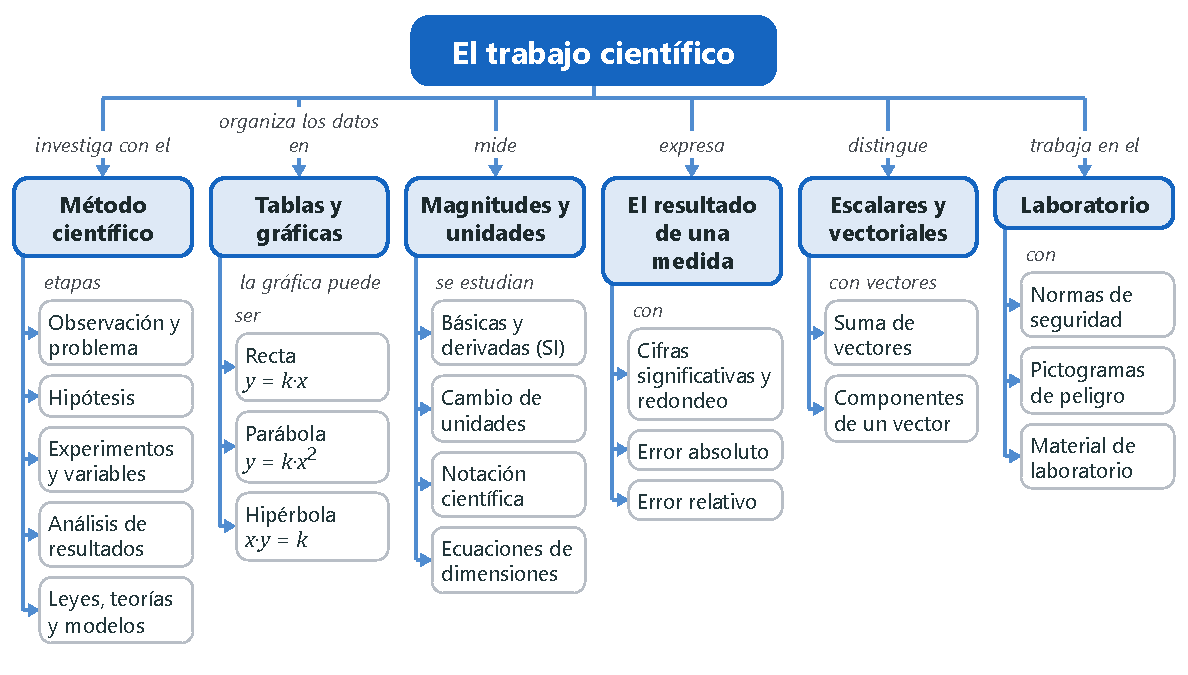
\includegraphics[width=\textwidth]{images/mapas_conceptuales/mapa_UD1}
\end{figure}

%========================================================================================
%\section*{Para empezar: Dorothy Hodgkin, bioquímica y cristalógrafa}
%\addcontentsline{toc}{section}{Para empezar: Dorothy Hodgkin, bioquímica y cristalógrafa}
%========================================================================================
%
%\textbf{Dorothy Hodgkin} (1910-1994) entró en la Universidad de Oxford en 1928, cuando la admisión de mujeres todavía estaba limitada. Se especializó en \textbf{cristalografía de rayos X}, una técnica entonces muy novedosa que permite averiguar la estructura de las moléculas, pero que exigía hacer a mano cálculos matemáticos larguísimos.
%
%En 1934 sorprendió con su trabajo sobre la estructura del colesterol, y se convirtió en la científica de referencia para «cartografiar» moléculas. Después se propuso averiguar la estructura de un antibiótico muy importante, la \textbf{penicilina}, descubierta por Alexander Fleming en 1928: los químicos necesitaban conocerla para poder fabricarla en el laboratorio. En 1945, tras cuatro años de trabajo y de crear nuevas técnicas de investigación, lo consiguió, y con ello contribuyó a salvar millones de vidas. Además, ideó un programa informático para cartografiar moléculas más deprisa, con el que determinó también las estructuras de la vitamina B\textsubscript{12} y de la insulina. Por todos sus logros recibió el Premio Nobel de Química en 1964.
%
%Su historia tiene que ver con el \textbf{ODS 4} (\emph{Educación de calidad}), que busca una educación inclusiva y equitativa y evitar la brecha de género en las carreras científicas y técnicas, y con el \textbf{ODS 3} (\emph{Salud y bienestar}), al que contribuyó con sus descubrimientos.
%
%En esta unidad aprenderemos cómo trabajan los científicos: en qué consiste el método científico, cómo se organizan y representan los datos, qué son las magnitudes y sus unidades, cómo se expresa el resultado de una medida, qué diferencia hay entre magnitudes escalares y vectoriales y qué normas de seguridad hay que seguir en el laboratorio.
%
%\begin{exercise}
%    ¿Qué tuvo de especial el ingreso de Dorothy Hodgkin en la Universidad de Oxford? ¿En qué especialidad destacó?
%    \begin{solu}
%        Entró en 1928, cuando todavía estaba \textcolor{red}{limitada la admisión de mujeres} en la universidad. Destacó en la \textcolor{red}{cristalografía de rayos X}.
%    \end{solu}
%\end{exercise}
%
%\begin{exercise}
%    ¿Qué herramienta creó para trabajar más deprisa? ¿Qué moléculas cartografió?
%    \begin{solu}
%        Un \textcolor{red}{programa informático} para cartografiar estructuras moleculares. Determinó las estructuras del \textcolor{red}{colesterol, la penicilina, la vitamina B\textsubscript{12} y la insulina}.
%    \end{solu}
%\end{exercise}
%
%\begin{exercise}
%    ¿Quién descubrió la penicilina? ¿Por qué era tan importante conocer la estructura de moléculas como la penicilina o la insulina?
%    \begin{solu}
%        \textcolor{red}{Alexander Fleming}, en 1928. Conocer su estructura permitía \textcolor{red}{fabricarlas en el laboratorio} (sintetizarlas) en grandes cantidades.
%    \end{solu}
%\end{exercise}
%
%\begin{exercise}
%    ¿Han contribuido sus descubrimientos a salvar vidas? ¿Qué relación tienen con los ODS 3 y 4?
%    \begin{solu}
%        \textcolor{red}{Sí}: la fabricación de penicilina e insulina ha permitido curar infecciones y tratar la diabetes a millones de personas, lo que contribuye a una vida sana (ODS 3). Su carrera muestra la importancia de que mujeres y hombres tengan el mismo acceso a la educación científica (ODS 4).
%    \end{solu}
%\end{exercise}

%========================================================================================
\section{¿En qué consiste el método científico?}
%========================================================================================

La \textbf{actividad científica} consiste en descubrir las leyes que rigen la naturaleza. Para ello se sigue un conjunto de etapas comunes a toda investigación, que llamamos \textbf{método científico} (figura~\ref{fig:metodo_cientifico}).

\begin{figure}[H]
    \centering
    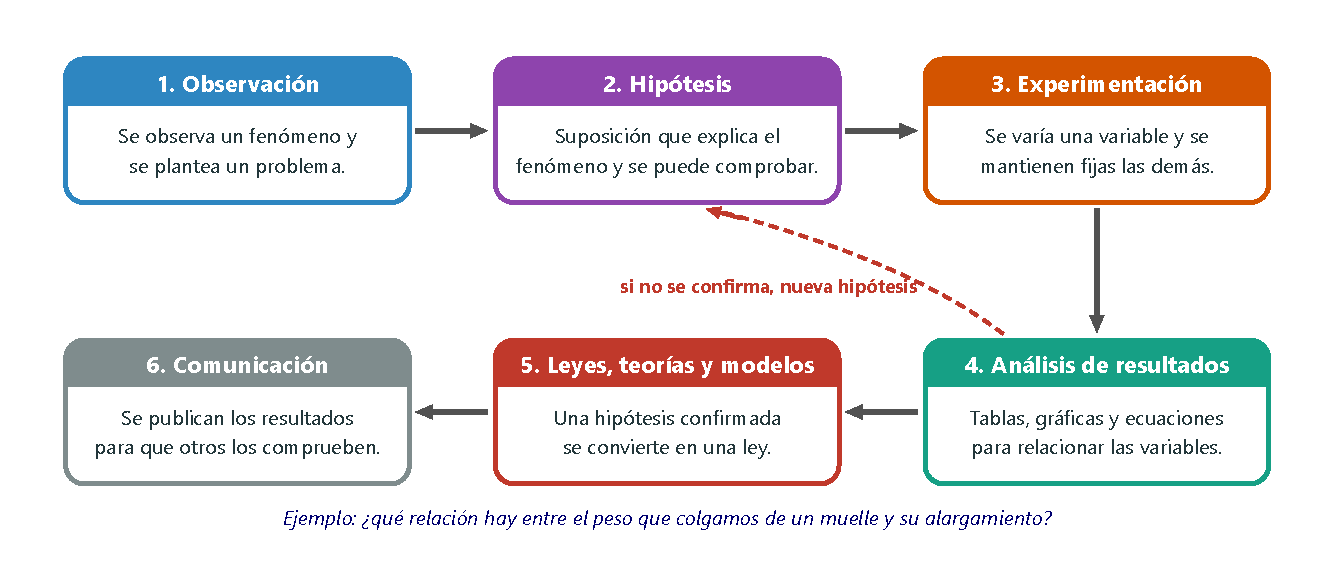
\includegraphics[width=\textwidth]{images/UD1/metodo_cientifico}
    \caption{Etapas del método científico.}
    \label{fig:metodo_cientifico}
\end{figure}

\subsection{Observación y planteamiento del problema}

Se observa con cuidado uno o más hechos o fenómenos con la intención de interpretarlos, lo que lleva a plantear preguntas. Por ejemplo, si colgamos una masa del extremo de un muelle, vemos que el muelle se alarga, y nos preguntamos: \emph{¿qué relación hay entre el peso que colgamos del muelle y el alargamiento que se produce?}

\subsection{Planteamiento de hipótesis}

\begin{definition}[Hipótesis científica]
    Una \textbf{hipótesis} es una suposición que intenta explicar un fenómeno. Para ser válida debe:
    \begin{itemize}
        \item Referirse a una situación real.
        \item Formularse de la forma más precisa posible, mediante variables concretas.
        \item Poder comprobarse experimentalmente, directamente o a través de sus consecuencias.
    \end{itemize}
\end{definition}

En el ejemplo, la hipótesis podría ser: \emph{el alargamiento del muelle es proporcional a la fuerza que se ejerce sobre él}.

\subsection{La experimentación}

Para saber si la hipótesis es cierta hay que comprobarla con hechos experimentales.

\begin{definition}[Experimentación y variables]
    La \textbf{experimentación} es la observación de un fenómeno en condiciones controladas.
    \begin{itemize}
        \item La \textbf{variable independiente} es la que el investigador va modificando.
        \item La \textbf{variable dependiente} es la que cambia como consecuencia y se mide para cada valor de la independiente.
        \item Las \textbf{variables controladas} son todas las demás, que deben mantenerse constantes.
    \end{itemize}
\end{definition}

Para comprobar nuestra hipótesis colgamos pesos diferentes del muelle y medimos los alargamientos (figura~\ref{fig:muelle_experimento}). El alargamiento es la longitud del muelle estirado, \(l\), menos su longitud natural, \(l_0\). La variable independiente es el peso que colgamos, y la dependiente, el alargamiento, \(l - l_0\).

\begin{figure}[H]
    \centering
    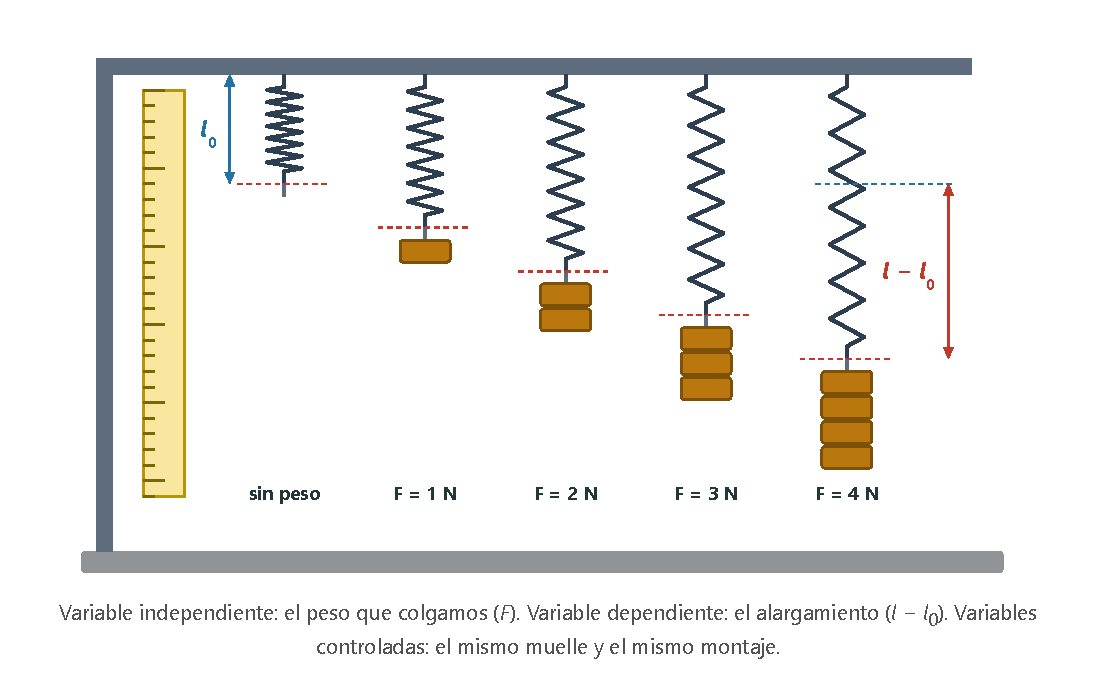
\includegraphics[width=0.85\textwidth]{images/UD1/muelle_experimento}
    \caption{Alargamiento de un muelle al colgar distintos pesos.}
    \label{fig:muelle_experimento}
\end{figure}

\subsection{Análisis de los resultados}

Los datos obtenidos se analizan para encontrar la relación entre las variables. Para ello se usan tablas, gráficas y otras herramientas matemáticas:

\begin{center}
    % --- tabla antigua ---
    % \begin{tblr}{colspec={lccccc}, hlines, vlines, row{1}={bg=ocre!85, fg=white, font=\bfseries}, column{1}={bg=ocre!85, fg=white, font=\bfseries}}
        % Fuerza, \(F\) (N) & \num{1.0} & \num{1.5} & \num{2.0} & \num{3.0} & \num{4.0} \\
        % Alargamiento, \(l - l_0\) (m) & \num{1.0e-2} & \num{1.5e-2} & \num{2.0e-2} & \num{3.0e-2} & \num{4.0e-2} \\
        % \(F/(l - l_0)\) (\unit{\newton\per\m}) & 100 & 100 & 100 & 100 & 100 \\
    % \end{tblr}
    % --- tabla nueva ---
    \begin{tabular}{@{}lccccc@{}}
        \toprule
        \textbf{Fuerza, \(F\) (N)} & \textbf{\num{1.0}} & \textbf{\num{1.5}} & \textbf{\num{2.0}} & \textbf{\num{3.0}} & \textbf{\num{4.0}} \\
        \midrule
        \textbf{Alargamiento, \(l - l_0\) (m)} & \num{1.0e-2} & \num{1.5e-2} & \num{2.0e-2} & \num{3.0e-2} & \num{4.0e-2} \\[3pt]
        \textbf{\(F/(l - l_0)\) (\unit{\newton\per\m})} & 100 & 100 & 100 & 100 & 100 \\
        \bottomrule
    \end{tabular}
\end{center}

\begin{center}
    \begin{tikzpicture}
        \begin{axis}[grafica, xlabel={alargamiento, \(x\) (m)}, ylabel={\(F\) (N)}, xmin=0, xmax=0.045, ymin=0, ymax=4.5, scaled x ticks=false, xtick={0,0.01,0.02,0.03,0.04}, xticklabels={0, \num{1e-2}, \num{2e-2}, \num{3e-2}, \num{4e-2}}]
            \addplot coordinates {(0,0) (0.01,1) (0.015,1.5) (0.02,2) (0.03,3) (0.04,4)};
        \end{axis}
    \end{tikzpicture}
\end{center}

El cociente entre la fuerza y el alargamiento es constante y la gráfica es una recta que pasa por el origen: las dos magnitudes son \textbf{directamente proporcionales} y la hipótesis queda confirmada.

\subsection{Elaboración de leyes, teorías y modelos científicos}

Una vez analizados los resultados, se puede establecer una relación matemática entre los hechos observados.

\begin{definition}[Ley, teoría y modelo]
    Los resultados de la investigación científica se organizan en leyes, teorías y modelos:
    \begin{itemize}
        \item Una \textbf{ley científica} es una hipótesis confirmada. En el ejemplo, la relación entre el alargamiento del muelle, \(x\), y la fuerza aplicada, \(F\), es la \textbf{ley de Hooke}: \(F = k \cdot x\).
        \item Una \textbf{teoría científica} es un conjunto de leyes que explica las regularidades descritas por ellas.
        \item Un \textbf{modelo científico} es una representación mental simplificada que se usa para explicar algunos fenómenos. Por ejemplo, los modelos atómicos de Thomson, Rutherford y Bohr.
    \end{itemize}
\end{definition}

Por último, los resultados se \textbf{comunican} (en revistas científicas, congresos\ldots) para que otros investigadores puedan comprobarlos, criticarlos y ampliarlos.

\subsection{¿Qué diferencia hay entre causalidad y correlación?}

\begin{itemize}
    \item La \textbf{causalidad} es la relación entre una causa y su efecto. Por ejemplo, al aumentar la presión sobre un gas encerrado en un recipiente con un émbolo móvil (causa), su volumen disminuye (efecto).
    \item La \textbf{correlación} solo indica que dos variables cambian a la vez, sin que una sea necesariamente la causa de la otra. Por ejemplo, si dejamos caer desde la misma altura una bolita metálica y una hoja de papel de la misma masa, la bolita llega antes. Pero eso no significa que el tiempo de caída dependa de la masa (las dos tienen la misma): influye otro factor, la superficie de los cuerpos, que determina el rozamiento con el aire.
\end{itemize}

\subsection*{Actividades de consolidación: el método científico}

\begin{exercise}
    Todo lo que sucede en el universo se puede organizar y explicar con unas pocas leyes.
    \begin{enumerate}[label=\alph*)]
        \item Enuncia algunas leyes que conozcas.
        \item Además de la elaboración de leyes, teorías y modelos, ¿qué otras etapas tiene el método científico?
        \item Mariano Barbacid, María Blasco, Montserrat Calleja, Avelino Corma, Francis Mojica, Margarita Salas o Rafael Yuste destacan por sus investigaciones. Elige dos e investiga sus aportaciones a la ciencia.
        \item ¿Qué hipótesis se pueden plantear para responder a esta pregunta: ¿cómo afecta la temperatura a la solubilidad del azúcar en agua?
    \end{enumerate}
    \begin{solu}
        a) Respuesta abierta: las \textcolor{red}{leyes de Newton}, la ley de \textcolor{red}{gravitación universal}, la ley de \textcolor{red}{Hooke}, las leyes de los gases (\textcolor{red}{Boyle, Gay-Lussac}), la ley de conservación de la masa\ldots
        b) \textcolor{red}{Observación} y planteamiento del problema, \textcolor{red}{hipótesis}, \textcolor{red}{experimentación}, \textcolor{red}{análisis} de resultados y \textcolor{red}{comunicación}.
        c) Respuesta libre. Por ejemplo, Margarita Salas descubrió cómo se copia el ADN de un virus (la ADN polimerasa del fago \(\phi\)29), base de una técnica muy usada para amplificar ADN; Francis Mojica descubrió las secuencias CRISPR, que han dado lugar a una herramienta de edición genética.
        d) Por ejemplo: «la solubilidad del azúcar en agua \textcolor{red}{aumenta} al aumentar la temperatura», o bien «\textcolor{red}{disminuye}» o «\textcolor{red}{no cambia}». Para comprobarla, se mide cuánto azúcar se disuelve en la misma cantidad de agua a distintas temperaturas.
    \end{solu}
\end{exercise}

\begin{exercise}
    Para averiguar si el período de un péndulo (el tiempo que tarda en ir y volver) depende de la longitud del hilo, se mide con dos longitudes, \qty{0.5}{\m} y \qty{1.0}{\m}, manteniendo la misma masa. En tres medidas con cada péndulo se obtiene siempre \qty{1.42}{\s} para el de \qty{0.5}{\m} y \qty{2.00}{\s} para el de \qty{1.0}{\m}.
    \begin{enumerate}[label=\alph*)]
        \item Identifica la variable independiente, la dependiente y la controlada.
        \item ¿Varía el período al variar la longitud? ¿Crees que hay una relación de causalidad?
        \item Quieres comprobar si el período depende de la masa. ¿Cuál es tu hipótesis? ¿Cómo la comprobarías?
        \item Un compañero dice que, cerca del ecuador, los péndulos oscilan más despacio que en países del norte, y que se debe a la temperatura. Busca información y respóndele de forma científica.
    \end{enumerate}
    \begin{solu}
        a) Independiente: la \textcolor{red}{longitud} del hilo. Dependiente: el \textcolor{red}{período}. Controlada: la \textcolor{red}{masa} (y la amplitud de las oscilaciones).
        b) \textcolor{red}{Sí}: al aumentar la longitud aumenta el período. Hay \textcolor{red}{causalidad}, porque solo se ha cambiado la longitud y las demás variables se han mantenido constantes.
        c) Hipótesis: «el período \textcolor{red}{no depende} de la masa». Se comprueba midiendo el período de péndulos de la \textcolor{red}{misma longitud} con \textcolor{red}{masas distintas}.
        d) El período es algo mayor cerca del ecuador, pero no por la temperatura, sino porque allí la \textcolor{red}{gravedad es algo menor} (por la rotación de la Tierra y porque el ecuador está más lejos del centro de la Tierra): cuanto menor es \(g\), mayor es el período (\(T = 2\pi\sqrt{L/g}\)).
    \end{solu}
\end{exercise}

\begin{exercise}
    Explica las diferencias entre variable dependiente, independiente y controlada.
    \begin{solu}
        La \textcolor{red}{independiente} es la que modifica el investigador; la \textcolor{red}{dependiente} es la que se mide, porque cambia como consecuencia de la anterior; las \textcolor{red}{controladas} son las demás, que se mantienen constantes durante el experimento.
    \end{solu}
\end{exercise}

\begin{exercise}
    A lo largo del siglo \textsc{xx}, científicos de distintos países investigaron la radiactividad y algunos participaron en proyectos de armas nucleares. Busca información sobre algunos de ellos y debatid en clase la responsabilidad de los científicos.
    \begin{solu}
        Respuesta libre. Por ejemplo: Henri Becquerel, Marie y Pierre Curie (descubrimiento de la radiactividad), Ernest Rutherford, Lise Meitner y Otto Hahn (fisión nuclear), Enrico Fermi, Robert Oppenheimer (Proyecto Manhattan) o Joseph Rotblat, que abandonó el proyecto y luchó por el desarme nuclear (Nobel de la Paz en 1995).
    \end{solu}
\end{exercise}

%========================================================================================
\section[Tablas de datos y gráficas]{¿Qué información aportan las tablas de datos y las representaciones gráficas?}
%========================================================================================

Una \textbf{tabla de datos} está formada por filas y columnas: cada columna (o fila) corresponde a una variable y cada medida ocupa una casilla. Con la tabla elaboramos una \textbf{representación gráfica}, que muestra la relación entre las variables. Normalmente, la \textbf{variable independiente} se sitúa en el eje horizontal o de abscisas (eje X), y la \textbf{variable dependiente}, en el eje vertical o de ordenadas (eje Y). La forma de la línea indica qué relación hay entre ellas.

\subsection{Si la gráfica es una línea recta}

Una recta que pasa por el origen indica que las variables son \textbf{directamente proporcionales}: \(y = a \cdot x\), donde \(a\) es la pendiente. Si la recta no pasa por el origen, la ecuación es \(y = a \cdot x + b\), donde \(b\) es la ordenada en el origen.

A partir de una gráfica podemos predecir valores entre los medidos (\textbf{interpolar}) o fuera de ellos (\textbf{extrapolar}).

\subsection{Si la gráfica es una parábola}

Una \textbf{parábola} que pasa por el origen indica que la variable dependiente es proporcional al \textbf{cuadrado} de la independiente: \(y = a \cdot x^2\) (o \(y = a \cdot x^2 + b\) si no pasa por el origen). Por ejemplo, la distancia que recorre un cuerpo que parte del reposo con aceleración constante.

\subsection{Si la gráfica es una hipérbola}

Una \textbf{hipérbola} indica que las variables son \textbf{inversamente proporcionales}: \(y = k/x\), es decir, su producto es constante. Por ejemplo, la presión y el volumen de un gas a temperatura constante (ley de Boyle): \(p \cdot V = k\).

\begin{center}
    \begin{tikzpicture}
        \begin{axis}[grafica, width=5.2cm, height=4.4cm, xmin=0, xmax=5, ymin=0, ymax=5.5, xticklabels={}, yticklabels={}, xlabel={\(x\)}, ylabel={\(y\)}, title={\small Recta: \(y = a \cdot x\)}]
            \addplot[mark=none, domain=0:5, line width=1.4pt, color=red!75!black] {x};
        \end{axis}
    \end{tikzpicture}
    \begin{tikzpicture}
        \begin{axis}[grafica, width=5.2cm, height=4.4cm, xmin=0, xmax=5, ymin=0, ymax=5.5, xticklabels={}, yticklabels={}, xlabel={\(x\)}, ylabel={\(y\)}, title={\small Parábola: \(y = a \cdot x^2\)}]
            \addplot[mark=none, domain=0:4.6, samples=50, line width=1.4pt, color=red!75!black] {x^2/4};
        \end{axis}
    \end{tikzpicture}
    \begin{tikzpicture}
        \begin{axis}[grafica, width=5.2cm, height=4.4cm, xmin=0, xmax=5, ymin=0, ymax=5.5, xticklabels={}, yticklabels={}, xlabel={\(x\)}, ylabel={\(y\)}, title={\small Hipérbola: \(y = k/x\)}]
            \addplot[mark=none, domain=0.4:5, samples=60, line width=1.4pt, color=red!75!black] {2/x};
        \end{axis}
    \end{tikzpicture}
\end{center}

\begin{example}
    Un entrenador cronometra a un atleta que corre en línea recta:
    \begin{center}
        % --- tabla antigua ---
        % \begin{tblr}{colspec={lccccc}, hlines, vlines, column{1}={bg=ocre!85, fg=white, font=\bfseries}}
            % Espacio, \(s\) (m) & 0 & 16 & 32 & 64 & 100 \\
            % Tiempo, \(t\) (s) & 0 & 4 & 8 & 16 & 25 \\
        % \end{tblr}
        % --- tabla nueva ---
        \begin{tabular}{@{}lccccc@{}}
            \toprule
            \textbf{Espacio, \(s\) (m)} & 0 & 16 & 32 & 64 & 100 \\[3pt]
            \textbf{Tiempo, \(t\) (s)} & 0 & 4 & 8 & 16 & 25 \\
            \bottomrule
        \end{tabular}
    \end{center}
    \begin{enumerate}[label=\alph*)]
        \item Representa el espacio recorrido en función del tiempo y escribe la ecuación que los relaciona.
        \item ¿Qué espacio habrá recorrido a los \qty{30}{\s}? ¿Cuánto tarda en recorrer los primeros \qty{12}{\m}?
    \end{enumerate}

    \begin{center}
        \begin{tikzpicture}
            \begin{axis}[grafica, xlabel={\(t\) (s)}, ylabel={\(s\) (m)}, xmin=0, xmax=32, ymin=0, ymax=130]
                \addplot coordinates {(0,0) (4,16) (8,32) (16,64) (25,100)};
                \addplot[mark=none, dashed, line width=1pt, color=blue!70!black] coordinates {(25,100) (30,120)};
            \end{axis}
        \end{tikzpicture}
    \end{center}

    a) La gráfica es una recta que pasa por el origen: \(s\) y \(t\) son directamente proporcionales. La pendiente es \(\dfrac{16}{4} = 4\), así que \textcolor{red}{\(s = 4 \cdot t\)} (con \(s\) en metros y \(t\) en segundos).

    b) Extrapolando: \(s = 4 \cdot 30 = \textcolor{red}{\qty{120}{\m}}\). Interpolando: \(12 = 4 \cdot t \Rightarrow t = \textcolor{red}{\qty{3}{\s}}\).
\end{example}

\begin{exercise}
    Se han medido las posiciones de un móvil a medida que transcurre el tiempo:
    \begin{center}
        % --- tabla antigua ---
        % \begin{tblr}{colspec={lcccccc}, hlines, vlines, column{1}={bg=ocre!85, fg=white, font=\bfseries}}
            % Posición, \(x\) (m) & 4 & 6 & 8 & 10 & 12 & 14 \\
            % Tiempo, \(t\) (s) & 0 & 1 & 2 & 3 & 4 & 5 \\
        % \end{tblr}
        % --- tabla nueva ---
        \begin{tabular}{@{}lcccccc@{}}
            \toprule
            \textbf{Posición, \(x\) (m)} & 4 & 6 & 8 & 10 & 12 & 14 \\[3pt]
            \textbf{Tiempo, \(t\) (s)} & 0 & 1 & 2 & 3 & 4 & 5 \\
            \bottomrule
        \end{tabular}
    \end{center}
    a) ¿En qué ejes situarías cada variable? b) Dibuja la gráfica posición-tiempo y escribe su ecuación.
    \begin{solu}
        a) El tiempo (variable independiente) en el \textcolor{red}{eje X}, y la posición (dependiente) en el \textcolor{red}{eje Y}.
        b) Es una \textcolor{red}{recta que no pasa por el origen}: pendiente \(\dfrac{2}{1} = 2\) y ordenada en el origen 4, así que \textcolor{red}{\(x = 4 + 2 \cdot t\)}.
        \begin{center}
            \begin{tikzpicture}
                \begin{axis}[grafica, width=6cm, height=4.2cm, xlabel={\(t\) (s)}, ylabel={\(x\) (m)}, xmin=0, xmax=5.5, ymin=0, ymax=16]
                    \addplot coordinates {(0,4) (1,6) (2,8) (3,10) (4,12) (5,14)};
                \end{axis}
            \end{tikzpicture}
        \end{center}
    \end{solu}
\end{exercise}

\subsection*{Actividades de consolidación: tablas de datos y gráficas}

\begin{exercise}
    En tres experimentos, las relaciones entre las variables son: a) \(y = 3x\); b) \(y = 10/x\); c) \(y = 5x^2\). ¿Qué forma tiene la gráfica de cada una? ¿Qué tipo de relación indica?
    \begin{solu}
        a) \textcolor{red}{Recta} que pasa por el origen: proporcionalidad directa.
        b) \textcolor{red}{Hipérbola}: proporcionalidad inversa.
        c) \textcolor{red}{Parábola}: \(y\) es proporcional al cuadrado de \(x\).
    \end{solu}
\end{exercise}

\begin{exercise}
    Estos son los valores de la velocidad de un móvil:
    \begin{center}
        % --- tabla antigua ---
        % \begin{tblr}{colspec={lcccc}, hlines, vlines, column{1}={bg=ocre!85, fg=white, font=\bfseries}}
            % Velocidad (m/s) & 0 & 3 & 6 & 9 \\
            % Tiempo (s) & 0 & 1 & 2 & 3 \\
        % \end{tblr}
        % --- tabla nueva ---
        \begin{tabular}{@{}lcccc@{}}
            \toprule
            \textbf{Velocidad (m/s)} & 0 & 3 & 6 & 9 \\[3pt]
            \textbf{Tiempo (s)} & 0 & 1 & 2 & 3 \\
            \bottomrule
        \end{tabular}
    \end{center}
    a) Dibuja la gráfica velocidad-tiempo. b) ¿Qué información proporciona? c) Escribe la ecuación que relaciona las variables. d) ¿En qué instantes la velocidad es \qty{4}{\m\per\s} y \qty{8}{\m\per\s}?
    \begin{solu}
        a) Una recta que pasa por el origen (tiempo en el eje X, velocidad en el eje Y).
        b) La velocidad y el tiempo son \textcolor{red}{directamente proporcionales}: la velocidad aumenta \qty{3}{\m\per\s} cada segundo.
        c) \textcolor{red}{\(v = 3 \cdot t\)}.
        d) \(4 = 3t \Rightarrow t = \textcolor{red}{\qty{1.33}{\s}}\); \(8 = 3t \Rightarrow t = \textcolor{red}{\qty{2.67}{\s}}\).
    \end{solu}
\end{exercise}

\begin{exercise}
    En un experimento con un gas a temperatura constante se obtienen estos datos. Comprueba que la presión y el volumen son inversamente proporcionales y calcula el volumen cuando la presión es \qty{2.5}{\atm}.
    \begin{center}
        % --- tabla antigua ---
        % \begin{tblr}{colspec={lcccc}, hlines, vlines, column{1}={bg=ocre!85, fg=white, font=\bfseries}}
            % Volumen (L) & \num{4.0} & \num{3.2} & \num{2.5} & \num{2.0} \\
            % Presión (atm) & \num{1.00} & \num{1.25} & \num{1.60} & \num{2.00} \\
        % \end{tblr}
        % --- tabla nueva ---
        \begin{tabular}{@{}lcccc@{}}
            \toprule
            \textbf{Volumen (L)} & \num{4.0} & \num{3.2} & \num{2.5} & \num{2.0} \\[3pt]
            \textbf{Presión (atm)} & \num{1.00} & \num{1.25} & \num{1.60} & \num{2.00} \\
            \bottomrule
        \end{tabular}
    \end{center}
    \begin{solu}
        El producto \(p \cdot V\) vale siempre \(\num{4.0}~\unit{\atm\liter}\) (\(1 \cdot 4 = \num{1.25} \cdot \num{3.2} = \num{1.6} \cdot \num{2.5} = 2 \cdot 2 = 4\)): son \textcolor{red}{inversamente proporcionales} (la gráfica es una hipérbola).
        \(V = \dfrac{4}{\num{2.5}} = \textcolor{red}{\qty{1.6}{\liter}}\).
    \end{solu}
\end{exercise}

%========================================================================================
\section[Magnitudes básicas y derivadas]{¿Qué es una magnitud? Magnitudes básicas y derivadas}
%========================================================================================

\begin{definition}[Magnitud y unidad]
    Una \textbf{magnitud} es cualquier propiedad de los cuerpos que se puede medir. \textbf{Medir} una magnitud es compararla con otra de la misma naturaleza, llamada \textbf{unidad}, para saber cuántas veces la contiene.
\end{definition}

Las \textbf{magnitudes básicas} se definen por sí mismas, mientras que las \textbf{magnitudes derivadas} se obtienen a partir de operaciones matemáticas con las básicas.

\subsection{El Sistema Internacional de Unidades (SI)}

\begin{center}
    % --- tabla antigua ---
    % \begin{tblr}{colspec={lccc}, hlines, vlines, row{1}={bg=ocre!85, fg=white, font=\bfseries\small}, cells={font=\small}}
        % Magnitud básica & Símbolo & Unidad & Símbolo \\
        % Longitud & \(L\) & metro & \unit{\m} \\
        % Masa & \(m\) & kilogramo & \unit{\kg} \\
        % Tiempo & \(t\) & segundo & \unit{\s} \\
        % Temperatura & \(T\) & kelvin & \unit{\kelvin} \\
        % Intensidad de corriente & \(I\) & amperio & \unit{\ampere} \\
        % Intensidad luminosa & \(I_v\) & candela & \unit{\candela} \\
        % Cantidad de sustancia & \(n\) & mol & \unit{\mol} \\
    % \end{tblr}
    % --- tabla nueva ---
    {\small
    \begin{tabular}{@{}lccc@{}}
        \toprule
        \textbf{Magnitud básica} & \textbf{Símbolo} & \textbf{Unidad} & \textbf{Símbolo} \\
        \midrule
        Longitud & \(L\) & metro & \unit{\m} \\[3pt]
        Masa & \(m\) & kilogramo & \unit{\kg} \\[3pt]
        Tiempo & \(t\) & segundo & \unit{\s} \\[3pt]
        Temperatura & \(T\) & kelvin & \unit{\kelvin} \\[3pt]
        Intensidad de corriente & \(I\) & amperio & \unit{\ampere} \\[3pt]
        Intensidad luminosa & \(I_v\) & candela & \unit{\candela} \\[3pt]
        Cantidad de sustancia & \(n\) & mol & \unit{\mol} \\
        \bottomrule
    \end{tabular}
    }
    \quad
    % --- tabla antigua ---
    % \begin{tblr}{colspec={lccc}, hlines, vlines, row{1}={bg=ocre!85, fg=white, font=\bfseries\small}, cells={font=\small}}
        % Magnitud derivada & Símbolo & Unidad SI & Otras \\
        % Superficie & \(S\) & \unit{\square\m} & -- \\
        % Volumen & \(V\) & \unit{\cubic\m} & L \\
        % Densidad & \(\rho\) & \unit{\kg\per\cubic\m} & g/mL \\
        % Velocidad & \(v\) & \unit{\m\per\s} & km/h \\
        % Aceleración & \(a\) & \unit{\m\per\square\s} & -- \\
        % Fuerza & \(F\) & N (newton) & -- \\
        % Presión & \(p\) & Pa (pascal) & atm, mmHg \\
        % Energía & \(E\) & J (julio) & eV \\
    % \end{tblr}
    % --- tabla nueva ---
    {\small
    \begin{tabular}{@{}lccc@{}}
        \toprule
        \textbf{Magnitud derivada} & \textbf{Símbolo} & \textbf{Unidad SI} & \textbf{Otras} \\
        \midrule
        Superficie & \(S\) & \unit{\square\m} & -- \\[3pt]
        Volumen & \(V\) & \unit{\cubic\m} & L \\[3pt]
        Densidad & \(\rho\) & \unit{\kg\per\cubic\m} & g/mL \\[3pt]
        Velocidad & \(v\) & \unit{\m\per\s} & km/h \\[3pt]
        Aceleración & \(a\) & \unit{\m\per\square\s} & -- \\[3pt]
        Fuerza & \(F\) & N (newton) & -- \\[3pt]
        Presión & \(p\) & Pa (pascal) & atm, mmHg \\[3pt]
        Energía & \(E\) & J (julio) & eV \\
        \bottomrule
    \end{tabular}
    }
\end{center}

Para expresar medidas muy grandes o muy pequeñas se usan los múltiplos y submúltiplos de las unidades, con estos prefijos:

\begin{center}
    % --- tabla antigua ---
    % \begin{tblr}{colspec={cccccc}, hlines, vlines, row{1}={bg=ocre!85, fg=white, font=\bfseries\small}, cells={font=\small}}
        % \num{e12} & \num{e9} & \num{e6} & \num{e3} & \num{e2} & \num{e1} \\
        % tera- (T) & giga- (G) & mega- (M) & kilo- (k) & hecto- (h) & deca- (da) \\
    % \end{tblr}
    % --- tabla nueva ---
    {\small
    \begin{tabular}{@{}cccccc@{}}
        \toprule
        \textbf{\num{e12}} & \textbf{\num{e9}} & \textbf{\num{e6}} & \textbf{\num{e3}} & \textbf{\num{e2}} & \textbf{\num{e1}} \\
        \midrule
        tera- (T) & giga- (G) & mega- (M) & kilo- (k) & hecto- (h) & deca- (da) \\
        \bottomrule
    \end{tabular}
    }
    \\[1ex]
    % --- tabla antigua ---
    % \begin{tblr}{colspec={cccccc}, hlines, vlines, row{1}={bg=ocre!85, fg=white, font=\bfseries\small}, cells={font=\small}}
        % \num{e-1} & \num{e-2} & \num{e-3} & \num{e-6} & \num{e-9} & \num{e-12} \\
        % deci- (d) & centi- (c) & mili- (m) & micro- (\(\mu\)) & nano- (n) & pico- (p) \\
    % \end{tblr}
    % --- tabla nueva ---
    {\small
    \begin{tabular}{@{}cccccc@{}}
        \toprule
        \textbf{\num{e-1}} & \textbf{\num{e-2}} & \textbf{\num{e-3}} & \textbf{\num{e-6}} & \textbf{\num{e-9}} & \textbf{\num{e-12}} \\
        \midrule
        deci- (d) & centi- (c) & mili- (m) & micro- (\(\mu\)) & nano- (n) & pico- (p) \\
        \bottomrule
    \end{tabular}
    }
\end{center}

\subsection{¿Cómo se transforman unas unidades en otras?}

Las medidas que no están en unidades del SI se transforman multiplicando por \textbf{factores de conversión}, fracciones que valen 1 (numerador y denominador expresan la misma cantidad):
\[ \qty{72}{\km\per\hour} = 72~\frac{\unit{\km}}{\unit{\hour}} \cdot \frac{\qty{e3}{\m}}{\qty{1}{\km}} \cdot \frac{\qty{1}{\hour}}{\qty{3600}{\s}} = \qty{20}{\m\per\s} \]
\[ \qty{11.34}{\gram\per\cubic\cm} = \num{11.34}~\frac{\unit{\gram}}{\unit{\cubic\cm}} \cdot \frac{\qty{1}{\kg}}{\qty{e3}{\gram}} \cdot \frac{\qty{e6}{\cubic\cm}}{\qty{1}{\cubic\m}} = \qty{11340}{\kg\per\cubic\m} \]

\subsection{¿Cómo se utiliza la notación científica?}

La \textbf{notación científica} consiste en escribir un número como un decimal con \textbf{una sola cifra entera} (distinta de cero) multiplicado por una \textbf{potencia de 10}, con exponente positivo o negativo. Para ello se desplaza la coma hasta que quede una sola cifra a su izquierda, y el número de lugares que se ha desplazado es el exponente:
\[ \qty{150000000000}{\m} = \qty{1.5e11}{\m} \qquad\qquad \qty{0.0000000002}{\m} = \qty{2e-10}{\m} \]
La distancia de la Tierra al Sol (\(1~\text{UA} = \qty{1.5e11}{\m}\)) se usa como unidad para las distancias del sistema solar, y el \textbf{año luz} (la distancia que recorre la luz en un año, unos \qty{9.46e15}{\m}), para las distancias entre estrellas y galaxias.

\begin{exercise}
    Transforma: a) a \unit{\m\per\s}: \qty{36}{\km\per\hour}, \qty{100}{\km\per\hour}, \qty{120}{\km\per\hour}; b) a \unit{\km\per\hour}: \qty{12}{\m\per\s}, \qty{340}{\m\per\s}, \qty{0.36}{\m\per\s}.
    \begin{solu}
        Para pasar de km/h a m/s se divide entre \num{3.6}, y al revés se multiplica.
        a) \textcolor{red}{\qty{10}{\m\per\s}}; \textcolor{red}{\qty{27.8}{\m\per\s}}; \textcolor{red}{\qty{33.3}{\m\per\s}}.
        b) \textcolor{red}{\qty{43.2}{\km\per\hour}}; \textcolor{red}{\qty{1224}{\km\per\hour}}; \textcolor{red}{\qty{1.3}{\km\per\hour}}.
    \end{solu}
\end{exercise}

\begin{exercise}
    Escribe en notación científica: a) \qty{0.00005}{\gram}; b) \qty{0.000052}{\gram}; c) \qty{2000000}{\m}; d) \qty{25000000}{\m}; e) \qty{3010000}{\s}; f) \qty{0.000205}{\ampere}.
    \begin{solu}
        a) \textcolor{red}{\qty{5e-5}{\gram}}; b) \textcolor{red}{\qty{5.2e-5}{\gram}}; c) \textcolor{red}{\qty{2e6}{\m}}; d) \textcolor{red}{\qty{2.5e7}{\m}}; e) \textcolor{red}{\qty{3.01e6}{\s}}; f) \textcolor{red}{\qty{2.05e-4}{\ampere}}.
    \end{solu}
\end{exercise}

\begin{exercise}
    Expresa en unidades del SI con notación científica: a) \qty{500}{\hecto\m}; b) \qty{3}{\deci\gram}; c) \qty{125}{\km}; d) \qty{250}{\gram}; e) \qty{25}{\mA}; f) \qty{1.25}{\cubic\dm}; g) \qty{9}{\us}; h) \qty{0.99}{\hecto\pascal}.
    \begin{solu}
        a) \textcolor{red}{\qty{5e4}{\m}}; b) \textcolor{red}{\qty{3e-4}{\kg}}; c) \textcolor{red}{\qty{1.25e5}{\m}}; d) \textcolor{red}{\qty{2.5e-1}{\kg}}; e) \textcolor{red}{\qty{2.5e-2}{\ampere}}; f) \textcolor{red}{\qty{1.25e-3}{\cubic\m}}; g) \textcolor{red}{\qty{9e-6}{\s}}; h) \textcolor{red}{\qty{99}{\pascal}} \(= \qty{9.9e1}{\pascal}\).
    \end{solu}
\end{exercise}

\begin{exercise}
    La densidad del argón es \qty{1.784}{\kg\per\cubic\m}. ¿Qué masa tiene \qty{1}{\cubic\cm} de argón?
    \begin{solu}
        \(\num{1.784}~\unit{\kg\per\cubic\m} = \num{1.784e-3}~\unit{\gram\per\cubic\cm}\); \(m = \rho \cdot V = \num{1.784e-3} \cdot 1 = \textcolor{red}{\qty{1.784e-3}{\gram}}\).
    \end{solu}
\end{exercise}

\begin{exercise}
    El récord de velocidad de un Fórmula 1, alcanzado en un entrenamiento en 2016, es de \qty{378}{\km\per\hour}. Exprésalo en \unit{\m\per\s}.
    \begin{solu}
        \(\dfrac{378}{\num{3.6}} = \textcolor{red}{\qty{105}{\m\per\s}}\).
    \end{solu}
\end{exercise}

\subsection*{Actividades de consolidación: magnitudes y unidades}

\begin{exercise}
    Clasifica en básicas o derivadas: densidad, longitud, volumen, masa, presión, temperatura, fuerza, trabajo, intensidad de corriente, superficie, energía, aceleración, cantidad de sustancia y velocidad.
    \begin{solu}
        Básicas: \textcolor{red}{longitud, masa, temperatura, intensidad de corriente y cantidad de sustancia}. Derivadas: \textcolor{red}{densidad, volumen, presión, fuerza, trabajo, superficie, energía, aceleración y velocidad}.
    \end{solu}
\end{exercise}

\begin{exercise}
    Escribe en notación científica y en unidades del SI:
    \begin{enumerate}[label=\alph*)]
        \item La distancia de la Tierra a la Luna: \qty{384400}{\km}.
        \item La distancia entre el átomo de hidrógeno y el de oxígeno en el agua: \qty{0.000000000097}{\m}.
        \item La distancia de Júpiter al Sol: \qty{778500000}{\km}.
        \item La masa de la Tierra: \qty{6000000000000000000000000}{\kg}.
        \item El tamaño de una bacteria: \qty{5}{\um}; el de un virus: \qty{24}{\nm}.
        \item El tiempo que tarda la luz del Sol en llegar a la Tierra: \qty{8}{\minute} \qty{20}{\s}.
    \end{enumerate}
    \begin{solu}
        a) \textcolor{red}{\qty{3.844e8}{\m}}; b) \textcolor{red}{\qty{9.7e-11}{\m}}; c) \textcolor{red}{\qty{7.785e11}{\m}}; d) \textcolor{red}{\qty{6e24}{\kg}}; e) \textcolor{red}{\qty{5e-6}{\m}}; \textcolor{red}{\qty{2.4e-8}{\m}}; f) \(8 \cdot 60 + 20 = \textcolor{red}{\qty{5.0e2}{\s}}\).
    \end{solu}
\end{exercise}

\begin{exercise}
    Expresa en notación científica: a) \qty{0.000008}{\ampere}; b) \qty{205000000}{\m}; c) \qty{0.00305}{\kg}; d) \qty{145000}{\s}.
    \begin{solu}
        a) \textcolor{red}{\qty{8e-6}{\ampere}}; b) \textcolor{red}{\qty{2.05e8}{\m}}; c) \textcolor{red}{\qty{3.05e-3}{\kg}}; d) \textcolor{red}{\qty{1.45e5}{\s}}.
    \end{solu}
\end{exercise}

\begin{exercise}
    La velocidad del sonido es \qty{1270}{\m\per\s} en el hidrógeno, \qty{927}{\m\per\s} en el helio, \qty{258}{\m\per\s} en el dióxido de carbono y \qty{340}{\m\per\s} en el aire. Exprésalas en \unit{\km\per\hour}.
    \begin{solu}
        Se multiplica por \num{3.6}: hidrógeno, \textcolor{red}{\qty{4572}{\km\per\hour}}; helio, \textcolor{red}{\qty{3337}{\km\per\hour}}; dióxido de carbono, \textcolor{red}{\qty{929}{\km\per\hour}}; aire, \textcolor{red}{\qty{1224}{\km\per\hour}}.
    \end{solu}
\end{exercise}

\begin{exercise}
    Expresa en unidades del SI con notación científica: a) \qty{300000}{\km\per\s}; b) \qty{2.5}{\hour}; c) \qty{10.5}{\gram\per\cubic\cm}. ¿Cuánto es la densidad media de la Tierra, \qty{5.51}{\gram\per\cubic\cm}, en unidades del SI?
    \begin{solu}
        a) \textcolor{red}{\qty{3e8}{\m\per\s}}; b) \(\num{2.5} \cdot 3600 = \textcolor{red}{\qty{9e3}{\s}}\); c) \textcolor{red}{\qty{1.05e4}{\kg\per\cubic\m}}. Tierra: \textcolor{red}{\qty{5510}{\kg\per\cubic\m}} \(= \qty{5.51e3}{\kg\per\cubic\m}\).
    \end{solu}
\end{exercise}

\begin{exercise}
    Un depósito cilíndrico tiene \qty{4}{\m} de altura y \qty{1}{\m} de radio. ¿Cuántos litros de agua contiene si el nivel está a \(1/3\) de la altura por debajo del borde superior?
    \begin{solu}
        La altura del agua es \(\frac{2}{3} \cdot 4 = \qty{2.67}{\m}\). \(V = \pi \cdot r^2 \cdot h = \pi \cdot 1^2 \cdot \num{2.67} = \qty{8.38}{\cubic\m} = \textcolor{red}{\qty{8378}{\liter}}\) (\(\approx \num{8.4e3}\) L).
    \end{solu}
\end{exercise}

\begin{exercise}
    La figura muestra el plano de una finca (cada cuadrado de la cuadrícula mide \(1 \times 1\)~\unit{\m}). Calcula su superficie dividiéndola en figuras sencillas.
    \begin{center}
        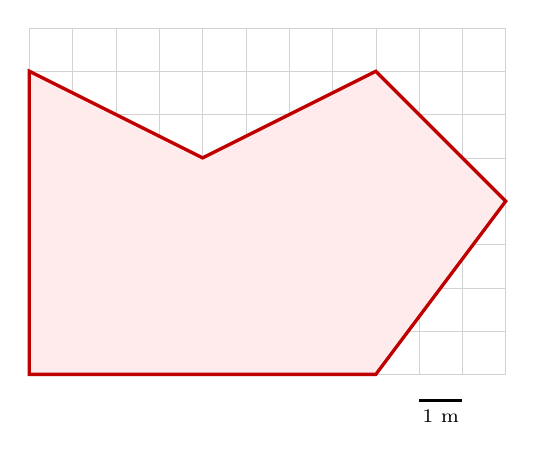
\begin{tikzpicture}[scale=0.55]
            \draw[step=1, gray!35, very thin] (0,0) grid (11,8);
            \draw[red!75!black, very thick, fill=red!8] (0,0) -- (8,0) -- (11,4) -- (8,7) -- (4,5) -- (0,7) -- cycle;
            \draw[thick] (9,-0.6) -- (10,-0.6); \node[below, font=\scriptsize] at (9.5,-0.6) {1 m};
        \end{tikzpicture}
    \end{center}
    \begin{solu}
        Partimos del rectángulo de \(8 \times 7\)~\unit{\m}: \(S_1 = 8 \cdot 7 = \qty{56}{\square\m}\).
        Le sumamos el triángulo de la derecha, de base 7 (el lado vertical \(x = 8\)) y altura 3: \(S_2 = \frac{1}{2} \cdot 7 \cdot 3 = \qty{10.5}{\square\m}\).
        Le restamos el triángulo de la muesca de arriba, de base 8 y altura 2: \(S_3 = \frac{1}{2} \cdot 8 \cdot 2 = \qty{8}{\square\m}\).
        \(S = 56 + \num{10.5} - 8 = \textcolor{red}{\qty{58.5}{\square\m}}\).
    \end{solu}
\end{exercise}

\begin{exercise}
    Indica la cantidad mayor de cada pareja: a) \qty{1600}{\gram} o \qty{1.5}{\kg}; b) \qty{1450}{\mm} o \qty{1.3}{\m}; c) \qty{320}{\s} o \qty{5}{\minute}; d) \qty{200}{\square\cm} o \qty{2}{\square\m}; e) \qty{0.000125}{\cubic\m} o \qty{125}{\cubic\m}.
    \begin{solu}
        a) \textcolor{red}{\qty{1600}{\gram}} (\qty{1.6}{\kg}); b) \textcolor{red}{\qty{1450}{\mm}} (\qty{1.45}{\m}); c) \textcolor{red}{\qty{320}{\s}} (\qty{5}{\minute} son \qty{300}{\s}); d) \textcolor{red}{\qty{2}{\square\m}}; e) \textcolor{red}{\qty{125}{\cubic\m}}.
    \end{solu}
\end{exercise}

\begin{exercise}
    Expresa en notación científica: a) \qty{60000000}{\m}; b) \qty{32000000}{\m}; c) \qty{9820000000}{\m}; d) \qty{570000}{\s}; e) \qty{0.005}{\s}; f) \qty{0.000075}{\kg}; g) \qty{0.00009}{\kg}; h) \qty{8000000000}{\kg}.
    \begin{solu}
        a) \textcolor{red}{\qty{6e7}{\m}}; b) \textcolor{red}{\qty{3.2e7}{\m}}; c) \textcolor{red}{\qty{9.82e9}{\m}}; d) \textcolor{red}{\qty{5.7e5}{\s}}; e) \textcolor{red}{\qty{5e-3}{\s}}; f) \textcolor{red}{\qty{7.5e-5}{\kg}}; g) \textcolor{red}{\qty{9e-5}{\kg}}; h) \textcolor{red}{\qty{8e9}{\kg}}.
    \end{solu}
\end{exercise}

%========================================================================================
\section{Ecuaciones de dimensiones}
%========================================================================================

Solo tiene sentido sumar o restar cantidades de la misma naturaleza: no podemos sumar una longitud y una temperatura. Para que una ecuación como \(A = B + C\) tenga sentido, \(A\), \(B\) y \(C\) deben tener las mismas \textbf{dimensiones}.

Las \textbf{dimensiones básicas} son las de las magnitudes básicas: longitud (L), masa (M), tiempo (T), intensidad de corriente (I), temperatura (\(\Theta\)), cantidad de sustancia (N) e intensidad luminosa (J). La \textbf{ecuación de dimensiones} de una magnitud expresa sus dimensiones en función de las básicas; se escribe el símbolo de la magnitud entre corchetes y se obtiene de su definición, prescindiendo de los números:
\[ [v] = \frac{[s]}{[t]} = \mathrm{L \cdot T^{-1}} \qquad [a] = \frac{[v]}{[t]} = \mathrm{L \cdot T^{-2}} \qquad [F] = [m] \cdot [a] = \mathrm{M \cdot L \cdot T^{-2}} \]

Las ecuaciones de dimensiones permiten comprobar si una ecuación física puede ser correcta: los dos miembros deben tener las mismas dimensiones (ecuación \textbf{homogénea}).

\begin{example}
    Comprueba que la ecuación de la fuerza centrípeta, \(F = \dfrac{m \cdot v^2}{r}\), es homogénea.

    Primer miembro: \([F] = \mathrm{M \cdot L \cdot T^{-2}}\). Segundo miembro: \(\dfrac{[m] \cdot [v]^2}{[r]} = \dfrac{\mathrm{M} \cdot (\mathrm{L \cdot T^{-1}})^2}{\mathrm{L}} = \mathrm{M \cdot L \cdot T^{-2}}\). Coinciden: \textcolor{red}{es homogénea}.
\end{example}

\begin{exercise}
    Escribe la ecuación de dimensiones del volumen y de la densidad.
    \begin{solu}
        \([V] = \textcolor{red}{\mathrm{L^3}}\); \([\rho] = \dfrac{[m]}{[V]} = \textcolor{red}{\mathrm{M \cdot L^{-3}}}\).
    \end{solu}
\end{exercise}

\begin{exercise}
    ¿Cuál de estas ecuaciones de dimensiones corresponde a la aceleración? a) \(\mathrm{L \cdot T^{-2}}\); b) \(\mathrm{L^{-2} \cdot T}\).
    \begin{solu}
        La \textcolor{red}{a)}: la aceleración es una velocidad (\(\mathrm{L \cdot T^{-1}}\)) dividida entre un tiempo.
    \end{solu}
\end{exercise}

\subsection*{Actividades de consolidación: ecuaciones de dimensiones}

\begin{exercise}
    ¿Qué es la ecuación de dimensiones de una magnitud? Pon un ejemplo.
    \begin{solu}
        Es la expresión de una magnitud en función de las \textcolor{red}{dimensiones básicas}. Por ejemplo, la velocidad es espacio entre tiempo: \([v] = \mathrm{L \cdot T^{-1}}\).
    \end{solu}
\end{exercise}

\begin{exercise}
    Comprueba que son homogéneas: a) espacio = velocidad \(\times\) tiempo; b) velocidad = aceleración \(\times\) tiempo; c) peso = masa \(\times\) aceleración de la gravedad.
    \begin{solu}
        a) \([s] = \mathrm{L}\); \([v] \cdot [t] = \mathrm{L \cdot T^{-1} \cdot T} = \mathrm{L}\). \textcolor{red}{Homogénea}.
        b) \([v] = \mathrm{L \cdot T^{-1}}\); \([a] \cdot [t] = \mathrm{L \cdot T^{-2} \cdot T} = \mathrm{L \cdot T^{-1}}\). \textcolor{red}{Homogénea}.
        c) \([P] = \mathrm{M \cdot L \cdot T^{-2}}\); \([m] \cdot [g] = \mathrm{M \cdot L \cdot T^{-2}}\). \textcolor{red}{Homogénea}.
    \end{solu}
\end{exercise}

\begin{exercise}
    No recuerdas la fórmula de la aceleración centrípeta y dudas entre: a) \(a = v/r^2\); b) \(a = v^2/r^2\); c) \(a = v/r\); d) \(a = v^2/r\). ¿Cómo puedes saber cuál es la correcta?
    \begin{solu}
        Comparando dimensiones con \([a] = \mathrm{L \cdot T^{-2}}\): a) \(\mathrm{L^{-1} T^{-1}}\); b) \(\mathrm{T^{-2}}\); c) \(\mathrm{T^{-1}}\); d) \(\dfrac{\mathrm{L^2 T^{-2}}}{\mathrm{L}} = \mathrm{L \cdot T^{-2}}\). Solo la \textcolor{red}{d)} es homogénea.
    \end{solu}
\end{exercise}

\begin{exercise}
    Relaciona cada magnitud con su ecuación de dimensiones: velocidad, aceleración, fuerza, volumen, superficie y densidad; \(\mathrm{L^3}\), \(\mathrm{L^2}\), \(\mathrm{M \cdot L^{-3}}\), \(\mathrm{L \cdot T^{-1}}\), \(\mathrm{M \cdot L \cdot T^{-2}}\), \(\mathrm{L \cdot T^{-2}}\).
    \begin{solu}
        Velocidad: \textcolor{red}{\(\mathrm{L \cdot T^{-1}}\)}; aceleración: \textcolor{red}{\(\mathrm{L \cdot T^{-2}}\)}; fuerza: \textcolor{red}{\(\mathrm{M \cdot L \cdot T^{-2}}\)}; volumen: \textcolor{red}{\(\mathrm{L^3}\)}; superficie: \textcolor{red}{\(\mathrm{L^2}\)}; densidad: \textcolor{red}{\(\mathrm{M \cdot L^{-3}}\)}.
    \end{solu}
\end{exercise}

\begin{exercise}
    La presión es una fuerza dividida entre una superficie, \(p = F/S\). ¿Cuál es su ecuación de dimensiones? a) \(\mathrm{M \cdot L^{-2} \cdot T^{-2}}\); b) \(\mathrm{M \cdot L^{-1} \cdot T^{-1}}\); c) \(\mathrm{M \cdot L^{-1} \cdot T^{-2}}\).
    \begin{solu}
        \([p] = \dfrac{\mathrm{M \cdot L \cdot T^{-2}}}{\mathrm{L^2}} = \mathrm{M \cdot L^{-1} \cdot T^{-2}}\): la \textcolor{red}{c)}.
    \end{solu}
\end{exercise}

%========================================================================================
\section[El resultado de una medida]{¿Cómo expresamos el resultado de una medida?}
%========================================================================================

\begin{definition}[Precisión]
    La \textbf{precisión} de un instrumento de medida es la menor variación de la magnitud que puede apreciar: el valor de la división más pequeña de su escala.
\end{definition}

La precisión de una medida se refleja en el número de cifras con que se expresa el resultado (figura~\ref{fig:precision}).

\begin{figure}[H]
    \centering
    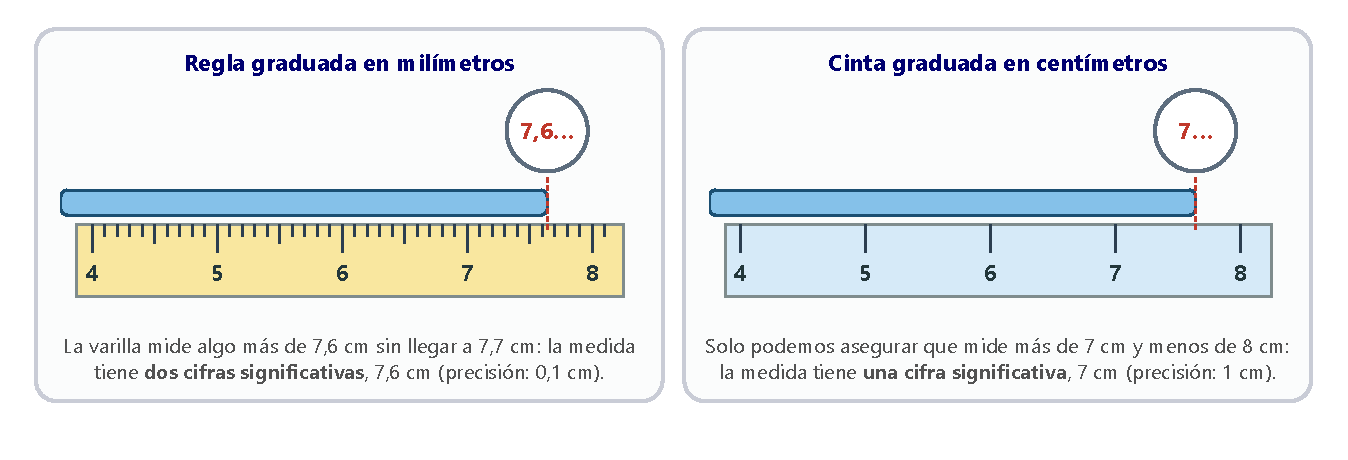
\includegraphics[width=\textwidth]{images/UD1/precision}
    \caption{La misma varilla medida con dos instrumentos de distinta precisión.}
    \label{fig:precision}
\end{figure}

\begin{definition}[Cifras significativas]
    Las \textbf{cifras significativas} de una medida son los dígitos que se conocen con seguridad.
\end{definition}

\begin{itemize}
    \item \textbf{Son significativas} todas las cifras distintas de cero (321 tiene tres; \num{1.345}, cuatro) y los ceros situados entre cifras distintas de cero o detrás de ellas en la parte decimal (\num{106.470} tiene seis).
    \item \textbf{No son significativos} los ceros a la izquierda de la primera cifra distinta de cero (\num{0.405} tiene tres; \num{0.0005090}, cuatro).
\end{itemize}

\subsection{El redondeo}

Al operar con medidas, el resultado no debe tener más cifras significativas que el dato que menos tenga. Se llama \textbf{redondeo} a la eliminación de las cifras situadas a la derecha de la última cifra significativa, con estas reglas:
\begin{itemize}
    \item Si la primera cifra que se elimina es \textbf{mayor que 5} (o un 5 seguido de otras cifras), la anterior aumenta en una unidad: \num{12.56} se redondea a \num{12.6}.
    \item Si es \textbf{menor que 5}, la anterior no cambia: \num{1.43} se redondea a \num{1.4}.
    \item Si es \textbf{exactamente 5}, la anterior aumenta en una unidad si es impar y se deja igual si es par (el cero se considera par): \num{10.35} se redondea a \num{10.4}, y \num{9.25}, a \num{9.2}.
\end{itemize}
Por ejemplo, \(\num{3.5432} + \num{2.531} = \num{6.0742}\), que redondeamos a \num{6.074}; y \(\num{2.33} \cdot \num{2.4} = \num{5.592}\), que redondeamos a \num{5.6}.

\subsection{Los errores en la medida}

Por mucho cuidado que tengamos, el valor medido nunca coincide exactamente con el valor verdadero: \textbf{toda medida está afectada por un error}.
\begin{itemize}
    \item Un \textbf{error accidental} se debe a causas imprevisibles y no aparece siempre (variaciones en las condiciones, apreciación del experimentador\ldots). Puede ser por exceso o por defecto, y se compensa en parte haciendo varias medidas y tomando la \textbf{media}.
    \item Un \textbf{error sistemático} aparece siempre que se mide, porque se debe a un mal funcionamiento del instrumento o al método de medida (por ejemplo, una balanza mal calibrada).
\end{itemize}

\begin{definition}[Error absoluto y error relativo]
    El \textbf{error absoluto}, \(\varepsilon_a\), es la diferencia entre el valor medido, \(x'\), y el valor verdadero, \(x\): \(\varepsilon_a = |x' - x|\). Tiene las mismas unidades que la magnitud.

    El \textbf{error relativo}, \(\varepsilon_r\), es el cociente entre el error absoluto y el valor verdadero: \(\varepsilon_r = \dfrac{\varepsilon_a}{x}\). No tiene unidades y suele expresarse en tanto por ciento. Una medida es más precisa cuanto menor es su error relativo.
\end{definition}

Como no conocemos el valor verdadero, tomamos como tal la \textbf{media} de varias medidas. Una medida no puede tener más cifras que las que indica su error: si medimos una hoja con una regla que aprecia milímetros y obtenemos \qty{28.8}{\cm}, el resultado es \(\num{28.8} \pm \qty{0.1}{\cm}\), no \(\num{28.83} \pm \qty{0.1}{\cm}\).

\begin{marker}
    \textbf{Cómo expresar el resultado de una medida directa:}
    \begin{enumerate}[label=\arabic*.]
        \item Se hacen varias medidas (al menos tres).
        \item Se calcula su media, \(x_\text{media}\), que se toma como valor verdadero.
        \item Se toma como error absoluto la precisión del instrumento.
        \item El resultado es \(x_\text{media} \pm \varepsilon_a\) (con su unidad), y se calcula el error relativo.
    \end{enumerate}
\end{marker}

\begin{example}
    Medimos el grosor de una moneda con un instrumento que aprecia \qty{0.01}{\mm} y obtenemos \qty{1.20}{\mm}, \qty{1.19}{\mm} y \qty{1.21}{\mm}. Expresa el resultado y calcula el error relativo.

    \[ x_\text{media} = \frac{\num{1.20} + \num{1.19} + \num{1.21}}{3} = \qty{1.20}{\mm} \]
    El resultado es \textcolor{red}{\(\num{1.20} \pm \qty{0.01}{\mm}\)}.
    \(\varepsilon_r = \dfrac{\num{0.01}}{\num{1.20}} = \num{8.3e-3} = \textcolor{red}{\qty{0.83}{\percent}}\).
\end{example}

\begin{exercise}
    Indica el número de cifras significativas: a) \qty{1525}{\kelvin}; b) \qty{3.0}{\kg}; c) \qty{0.125}{\ampere}; d) \qty{0.425}{\m}; e) \qty{5.1}{\s}; f) \qty{105.40}{\cm}; g) \qty{20.15}{\mL}; h) \qty{9.27}{\km}.
    \begin{solu}
        a) \textcolor{red}{4}; b) \textcolor{red}{2}; c) \textcolor{red}{3}; d) \textcolor{red}{3}; e) \textcolor{red}{2}; f) \textcolor{red}{5}; g) \textcolor{red}{4}; h) \textcolor{red}{3}.
    \end{solu}
\end{exercise}

\begin{exercise}
    Medimos la temperatura de una disolución con un termómetro cuya precisión es \qty{0.5}{\degreeCelsius}. a) ¿Podemos decir que la temperatura es \(\num{54.4} \pm \qty{0.5}{\degreeCelsius}\)? b) ¿Cómo la expresaríamos correctamente?
    \begin{solu}
        a) \textcolor{red}{No}: con una escala que va de medio en medio grado no podemos leer \num{54.4}; las lecturas posibles son \num{54.0}, \num{54.5}\ldots{} b) Por ejemplo, \textcolor{red}{\(\num{54.5} \pm \qty{0.5}{\degreeCelsius}\)}.
    \end{solu}
\end{exercise}

\begin{exercise}
    Medimos el grosor del lomo de un libro con una regla que aprecia milímetros y obtenemos \qty{19.0}{\mm}. a) ¿Cuál es el error absoluto? Expresa el resultado. b) Calcula el error relativo.
    \begin{solu}
        a) \(\varepsilon_a = \qty{1}{\mm}\); resultado: \textcolor{red}{\(19 \pm \qty{1}{\mm}\)}. b) \(\varepsilon_r = \dfrac{1}{19} \cdot 100 = \textcolor{red}{\qty{5.3}{\percent}}\).
    \end{solu}
\end{exercise}

\subsection*{Actividades de consolidación: la expresión de la medida}

\begin{exercise}
    Asocia cada concepto con su definición. Conceptos: redondeo, cifra significativa, error accidental, error sistemático, error absoluto, error relativo, valor verdadero.
    \begin{enumerate}[label=\alph*)]
        \item Error debido a una causa imprevisible que no se presenta siempre.
        \item Dígito que se conoce con seguridad en una medida.
        \item Error debido al mal funcionamiento del instrumento o al método de medida.
        \item Eliminación de las cifras situadas a la derecha de la última cifra significativa.
        \item En una medida directa, coincide con la precisión del instrumento.
        \item Media de todas las medidas realizadas.
        \item Cociente entre el error absoluto y el valor verdadero.
    \end{enumerate}
    \begin{solu}
        a) \textcolor{red}{Error accidental}; b) \textcolor{red}{cifra significativa}; c) \textcolor{red}{error sistemático}; d) \textcolor{red}{redondeo}; e) \textcolor{red}{error absoluto}; f) \textcolor{red}{valor verdadero}; g) \textcolor{red}{error relativo}.
    \end{solu}
\end{exercise}

\begin{exercise}
    ¿Cuántas cifras significativas tienen estas masas, en kg? a) 543; b) \num{5.622}; c) \num{42.0}; d) \num{105.320}; e) \num{0.05}; f) \num{9.29}.
    \begin{solu}
        a) \textcolor{red}{3}; b) \textcolor{red}{4}; c) \textcolor{red}{3}; d) \textcolor{red}{6}; e) \textcolor{red}{1}; f) \textcolor{red}{3}.
    \end{solu}
\end{exercise}

\begin{exercise}
    Redondea a una cifra decimal (en cm): a) \num{10.68}; b) \num{1.08}; c) \num{2.42}; d) \num{10.55}; e) \num{104.20}; f) \num{9.65}.
    \begin{solu}
        a) \textcolor{red}{\num{10.7}}; b) \textcolor{red}{\num{1.1}}; c) \textcolor{red}{\num{2.4}}; d) \textcolor{red}{\num{10.6}} (el 5 sigue a un 5, impar); e) \textcolor{red}{\num{104.2}}; f) \textcolor{red}{\num{9.6}} (el 5 sigue a un 6, par).
    \end{solu}
\end{exercise}

\begin{exercise}
    Un joyero mide varias veces la masa de una joya: \qty{4.25}{\gram}, \qty{4.28}{\gram}, \qty{4.27}{\gram}, \qty{4.23}{\gram}, \qty{4.26}{\gram}, \qty{4.27}{\gram} y \qty{4.26}{\gram}. a) Expresa el resultado con su error absoluto. b) Calcula el error relativo.
    \begin{solu}
        a) \(x_\text{media} = \dfrac{\num{29.82}}{7} = \qty{4.26}{\gram}\). La balanza aprecia centésimas de gramo, así que \(\varepsilon_a = \qty{0.01}{\gram}\): \textcolor{red}{\(\num{4.26} \pm \qty{0.01}{\gram}\)}.
        b) \(\varepsilon_r = \dfrac{\num{0.01}}{\num{4.26}} \cdot 100 = \textcolor{red}{\qty{0.23}{\percent}}\).
    \end{solu}
\end{exercise}

\begin{exercise}
    Con un péndulo simple determinamos la aceleración de la gravedad y obtenemos (en \unit{\m\per\square\s}): \num{9.82}, \num{9.84}, \num{9.89}, \num{9.79}, \num{9.91}, \num{9.83}. a) Calcula el valor medio y su error absoluto. b) Halla el error relativo.
    \begin{solu}
        a) \(g_\text{media} = \dfrac{\num{59.08}}{6} = \num{9.847} \approx \qty{9.85}{\m\per\square\s}\). Es una medida \emph{indirecta} (\(g\) se calcula a partir de otras medidas), así que no hay precisión de un aparato; tomamos como error la media de las desviaciones respecto al valor medio:
        \(\varepsilon_a = \dfrac{\num{0.03} + \num{0.01} + \num{0.04} + \num{0.06} + \num{0.06} + \num{0.02}}{6} = \num{0.04}\). Resultado: \textcolor{red}{\(\num{9.85} \pm \qty{0.04}{\m\per\square\s}\)}.
        b) \(\varepsilon_r = \dfrac{\num{0.04}}{\num{9.85}} \cdot 100 = \textcolor{red}{\qty{0.4}{\percent}}\).
    \end{solu}
\end{exercise}

\begin{exercise}
    Con una balanza digital que aprecia miligramos obtenemos (en g): \num{18.464}, \num{18.462}, \num{18.465}, \num{18.464}, \num{18.463}, \num{18.463}. a) Expresa el resultado. b) Calcula el error relativo.
    \begin{solu}
        a) \(x_\text{media} = \dfrac{\num{110.781}}{6} = \num{18.4635} \approx \qty{18.464}{\gram}\) (el 5 sigue a un 3, impar). Resultado: \textcolor{red}{\(\num{18.464} \pm \qty{0.001}{\gram}\)}.
        b) \(\varepsilon_r = \dfrac{\num{0.001}}{\num{18.464}} \cdot 100 = \textcolor{red}{\qty{0.0054}{\percent}}\).
    \end{solu}
\end{exercise}

\begin{exercise}
    Medimos la anchura de un móvil con una regla que aprecia milímetros y obtenemos \qty{7.0}{\cm}. a) ¿Cuál es el error absoluto? Expresa el resultado. b) Calcula el error relativo.
    \begin{solu}
        a) \(\varepsilon_a = \qty{0.1}{\cm}\): \textcolor{red}{\(\num{7.0} \pm \qty{0.1}{\cm}\)}. b) \(\varepsilon_r = \dfrac{\num{0.1}}{\num{7.0}} \cdot 100 = \textcolor{red}{\qty{1.4}{\percent}}\).
    \end{solu}
\end{exercise}

%========================================================================================
\section[Magnitudes escalares y vectoriales]{¿En qué se diferencian las magnitudes escalares de las vectoriales?}
%========================================================================================

Si leemos la temperatura en un termómetro, no necesitamos más información. Pero si nos dicen que un coche va a \qty{36}{\km\per\hour}, para saber dónde estará dentro de un rato necesitamos conocer también hacia dónde va.

\begin{definition}[Magnitudes escalares y vectoriales]
    Una \textbf{magnitud escalar} queda especificada completamente con un número y su unidad: la masa, la densidad, la temperatura, el tiempo, la presión, la energía\ldots{} Se opera con ellas siguiendo las reglas de la aritmética.

    Una \textbf{magnitud vectorial} queda definida por su \textbf{módulo} (valor numérico), su \textbf{dirección} (recta sobre la que actúa), su \textbf{sentido} y su \textbf{punto de aplicación}: la velocidad, la aceleración, la fuerza, el desplazamiento\ldots{} Se representan mediante \textbf{vectores}, con una flecha sobre el símbolo: \(\vec{v}\).
\end{definition}

Un \textbf{vector} es un segmento orientado: su longitud representa el módulo, la recta que lo contiene es la dirección, la punta de flecha indica el sentido y su origen es el punto de aplicación (figura~\ref{fig:vectores}). Dos vectores son \textbf{opuestos} si tienen el mismo módulo y la misma dirección, pero sentidos contrarios: \(\vec{a} = -\vec{b}\).

\begin{figure}[H]
    \centering
    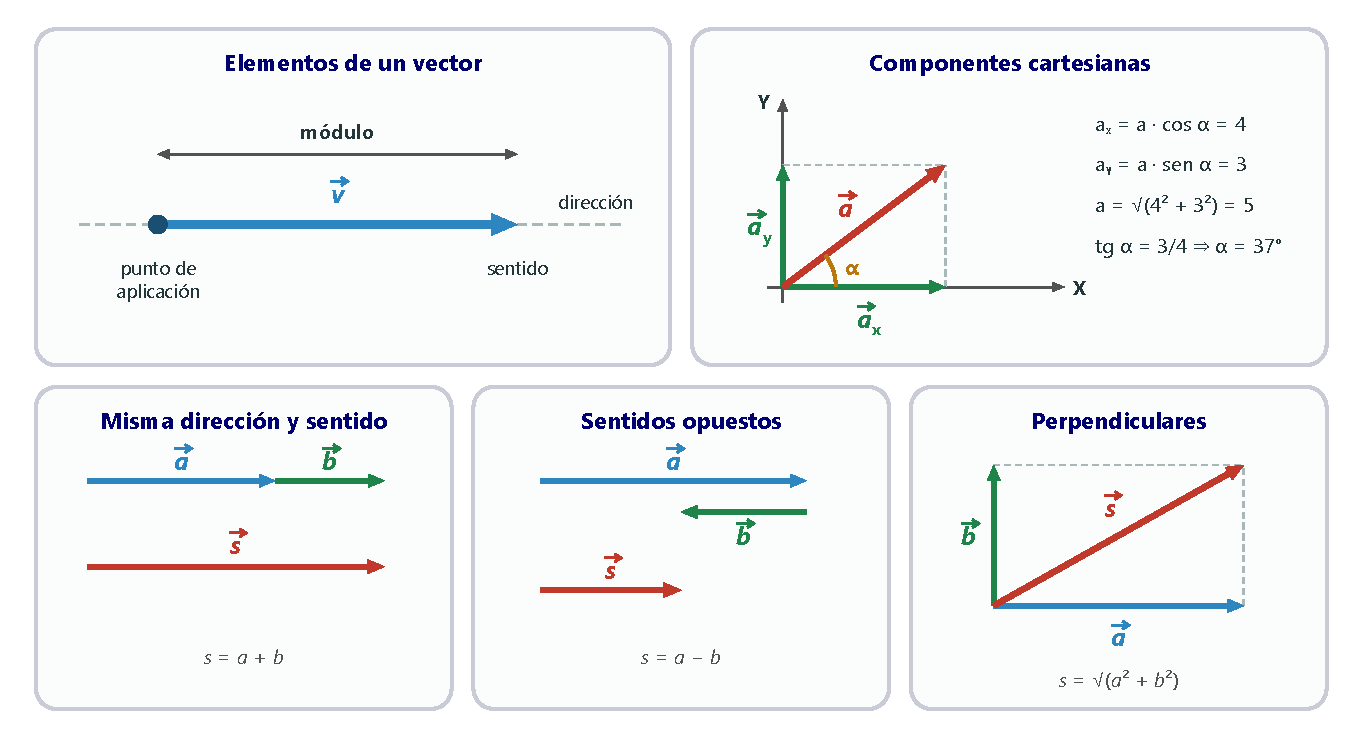
\includegraphics[width=\textwidth]{images/UD1/vectores}
    \caption{Elementos de un vector, componentes cartesianas y suma de vectores.}
    \label{fig:vectores}
\end{figure}

\subsection{¿Cómo se suman los vectores?}

Para sumar dos vectores, se traslada el segundo paralelamente a sí mismo hasta que su origen coincida con el extremo del primero; el vector suma va desde el origen del primero hasta el extremo del segundo. Si los dos vectores tienen el mismo punto de aplicación, la suma es la diagonal del paralelogramo que forman (\textbf{regla del paralelogramo}). Casos particulares (figura~\ref{fig:vectores}):
\begin{itemize}
    \item \textbf{Misma dirección y sentido}: el módulo de la suma es la suma de los módulos, \(s = a + b\), con la misma dirección y sentido.
    \item \textbf{Misma dirección y sentidos opuestos}: el módulo de la suma es la diferencia de los módulos, \(s = a - b\), con el sentido del mayor.
    \item \textbf{Perpendiculares}: por el teorema de Pitágoras, \(s = \sqrt{a^2 + b^2}\).
\end{itemize}

\subsection{¿Cuáles son las componentes de un vector?}

Cualquier vector puede expresarse como la suma de un vector en el eje X y otro en el eje Y, sus \textbf{componentes cartesianas}: \(\vec{a} = \vec{a}_x + \vec{a}_y\). Si \(\alpha\) es el ángulo que forma con el eje X:
\[ a_x = a \cdot \cos\alpha \qquad a_y = a \cdot \sen\alpha \qquad a = \sqrt{a_x^2 + a_y^2} \qquad \tg\alpha = \frac{a_y}{a_x} \]
Por ejemplo, un vector de módulo 5 que forma \ang{37} con el eje X tiene componentes \(a_x = 4\) y \(a_y = 3\).

\begin{exercise}
    Clasifica en escalares y vectoriales: masa, temperatura, velocidad, tiempo, aceleración y fuerza. Escribe dos ejemplos más de cada tipo.
    \begin{solu}
        Escalares: \textcolor{red}{masa, temperatura y tiempo} (otras: energía, volumen). Vectoriales: \textcolor{red}{velocidad, aceleración y fuerza} (otras: desplazamiento, peso).
    \end{solu}
\end{exercise}

\begin{exercise}
    Dibuja un vector con origen en el origen de coordenadas, de módulo 4, dirección la del eje X y sentido hacia las \(x\) positivas. Dibuja después su opuesto.
    \begin{solu}
        \begin{center}
            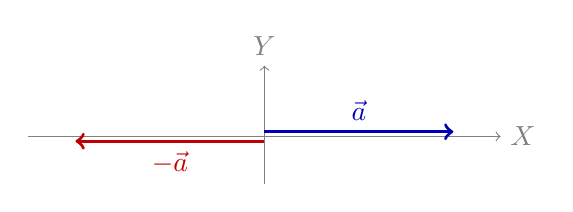
\begin{tikzpicture}[scale=0.6]
                \draw[->, gray] (-5,0) -- (5,0) node[right] {\(X\)}; \draw[->, gray] (0,-1) -- (0,1.5) node[above] {\(Y\)};
                \draw[->, very thick, blue!70!black] (0,0.1) -- (4,0.1) node[above, pos=0.5] {\(\vec{a}\)};
                \draw[->, very thick, red!75!black] (0,-0.1) -- (-4,-0.1) node[below, pos=0.5] {\(-\vec{a}\)};
            \end{tikzpicture}
        \end{center}
        El opuesto tiene el \textcolor{red}{mismo módulo y dirección, pero sentido contrario}.
    \end{solu}
\end{exercise}

\begin{exercise}
    Calcula el módulo de los vectores de componentes: a) \(a_x = 5\), \(a_y = 5\); b) \(b_x = 5\), \(b_y = 7\); c) \(c_x = -5\), \(c_y = -7\). Halla el ángulo que forma cada uno con el eje X.
    \begin{solu}
        a) \(a = \sqrt{25 + 25} = \textcolor{red}{\num{7.07}}\); \(\tg\alpha = 1 \Rightarrow \alpha = \textcolor{red}{\ang{45}}\).
        b) \(b = \sqrt{25 + 49} = \textcolor{red}{\num{8.60}}\); \(\tg\alpha = \num{1.4} \Rightarrow \alpha = \textcolor{red}{\ang{54.5}}\).
        c) \(c = \textcolor{red}{\num{8.60}}\); apunta hacia el tercer cuadrante: \(\alpha = \ang{180} + \ang{54.5} = \textcolor{red}{\ang{234.5}}\).
    \end{solu}
\end{exercise}

\begin{exercise}
    Dibuja dos vectores con el mismo punto de aplicación, direcciones perpendiculares y uno de módulo triple que el otro. Si el menor mide 2, ¿cuánto mide su suma?
    \begin{solu}
        Por ejemplo, \(\vec{a}\) de módulo 2 en el eje X y \(\vec{b}\) de módulo 6 en el eje Y. \(s = \sqrt{2^2 + 6^2} = \textcolor{red}{\num{6.32}}\).
    \end{solu}
\end{exercise}

\subsection*{Actividades de consolidación: magnitudes escalares y vectoriales}

\begin{exercise}
    Clasifica en escalares y vectoriales: presión, volumen, temperatura, masa, densidad, velocidad, aceleración, aceleración de la gravedad, tiempo, desplazamiento, potencia y energía térmica.
    \begin{solu}
        Escalares: \textcolor{red}{presión, volumen, temperatura, masa, densidad, tiempo, potencia y energía térmica}. Vectoriales: \textcolor{red}{velocidad, aceleración, aceleración de la gravedad y desplazamiento}.
    \end{solu}
\end{exercise}

\begin{exercise}
    ¿Qué elementos tiene un vector? ¿Por qué se dice que la fuerza es una magnitud vectorial? Indica si cada descripción corresponde a una magnitud escalar o vectorial: a) hay que especificar su punto de aplicación; b) se cuantifica con un número y su unidad; c) se representa con un vector; d) hay que especificar su dirección y sentido.
    \begin{solu}
        \textcolor{red}{Módulo, dirección, sentido y punto de aplicación}. La fuerza es vectorial porque su efecto depende también de hacia dónde y dónde se aplica. Escalar: \textcolor{red}{b)}; vectorial: \textcolor{red}{a), c) y d)}.
    \end{solu}
\end{exercise}

\begin{exercise}
    Calcula la suma de dos vectores de módulos 7 y 9 aplicados en el mismo punto si: a) tienen la misma dirección y sentido; b) la misma dirección y sentidos opuestos; c) son perpendiculares.
    \begin{solu}
        a) \(7 + 9 = \textcolor{red}{16}\); b) \(9 - 7 = \textcolor{red}{2}\), en el sentido del de módulo 9; c) \(\sqrt{49 + 81} = \textcolor{red}{\num{11.4}}\).
    \end{solu}
\end{exercise}

\begin{exercise}
    Tres vectores están aplicados en el origen: \(\vec{a}\), de módulo 3, apunta hacia las \(x\) positivas; \(\vec{b}\), de módulo 3, hacia las \(x\) negativas; \(\vec{c}\), de módulo 5, hacia las \(y\) negativas. a) ¿Qué vectores tienen la misma dirección? ¿Y el mismo módulo? b) Describe el opuesto de \(\vec{c}\). c) Calcula \(\vec{a} + \vec{b}\) y \(\vec{a} + \vec{c}\).
    \begin{solu}
        a) \(\vec{a}\) y \(\vec{b}\) tienen la \textcolor{red}{misma dirección} (eje X) y el \textcolor{red}{mismo módulo}, pero sentidos opuestos: son opuestos.
        b) \(-\vec{c}\): módulo 5, dirección del eje Y, \textcolor{red}{sentido hacia las \(y\) positivas}.
        c) \(\vec{a} + \vec{b} = \vec{0}\) (módulo \textcolor{red}{0}); \(|\vec{a} + \vec{c}| = \sqrt{9 + 25} = \textcolor{red}{\num{5.83}}\).
    \end{solu}
\end{exercise}

\begin{exercise}
    Los vectores \(\vec{a}\) (módulo 2) y \(\vec{b}\) (módulo 3) apuntan hacia la derecha, y \(\vec{c}\) (módulo 6), hacia la izquierda, todos en la misma dirección. Calcula: a) \(\vec{a} + \vec{b}\); b) \(\vec{a} + \vec{b} + \vec{c}\); c) \(\vec{b} - \vec{a}\).
    \begin{solu}
        a) Módulo \textcolor{red}{5}, hacia la derecha. b) \(5 - 6\): módulo \textcolor{red}{1}, hacia la izquierda. c) Módulo \textcolor{red}{1}, hacia la derecha.
    \end{solu}
\end{exercise}

\begin{exercise}
    a) Calcula la suma de dos vectores perpendiculares de módulo 50 aplicados en el mismo punto. b) La suma de dos vectores perpendiculares vale \num{8.6} y uno mide 5. ¿Cuánto mide el otro? c) ¿Cuánto vale la suma de dos vectores de módulos 3 y 4 si son paralelos del mismo sentido, de sentido opuesto o perpendiculares?
    \begin{solu}
        a) \(\sqrt{50^2 + 50^2} = \textcolor{red}{\num{70.7}}\).
        b) \(\num{8.6}^2 = 5^2 + b^2 \Rightarrow b = \sqrt{\num{73.96} - 25} = \textcolor{red}{7}\).
        c) \textcolor{red}{7}; \textcolor{red}{1}; \(\sqrt{9 + 16} = \textcolor{red}{5}\).
    \end{solu}
\end{exercise}

%========================================================================================
\section[El laboratorio de física y química]{Normas de seguridad en el laboratorio de física y química}
%========================================================================================

Los laboratorios de física y química están preparados para experimentar e investigar. Tienen agua corriente, electricidad y a veces gas, mesas y armarios adecuados, campanas extractoras de gases, extintores, lavaojos y un botiquín. Para evitar accidentes hay que seguir estas normas:

\begin{enumerate}[label=\numberballblue]
    \item Localiza las salidas de emergencia, los extintores, los lavaojos y los equipos de emergencia. No corras dentro del laboratorio.
    \item Mantén el área de trabajo limpia, ordenada y con solo el material que vayas a usar.
    \item Usa bata (abrochada) y guantes; y gafas de seguridad cuando manejes productos tóxicos o corrosivos.
    \item Maneja el material de vidrio con cuidado. Si se rompe, deposítalo en el contenedor para vidrio, nunca en la papelera.
    \item No manipules sustancias inflamables cerca de fuentes de calor. Calienta los tubos de ensayo con pinzas de madera, inclinados y sin apuntar con ellos a nadie.
    \item No toques aparatos eléctricos con las manos mojadas ni los dejes cerca de líquidos.
    \item No comas ni bebas en el laboratorio, y lávate las manos al salir.
    \item Trabaja en la campana extractora con las sustancias o reacciones que desprenden gases.
    \item No viertas residuos por el desagüe, sino en los recipientes destinados a ellos, y no devuelvas los restos de reactivo a los frascos originales.
    \item No pipetees nunca con la boca: usa una pera o un pipeteador. Tapa los frascos después de usarlos.
\end{enumerate}

\begin{figure}[H]
    \centering
    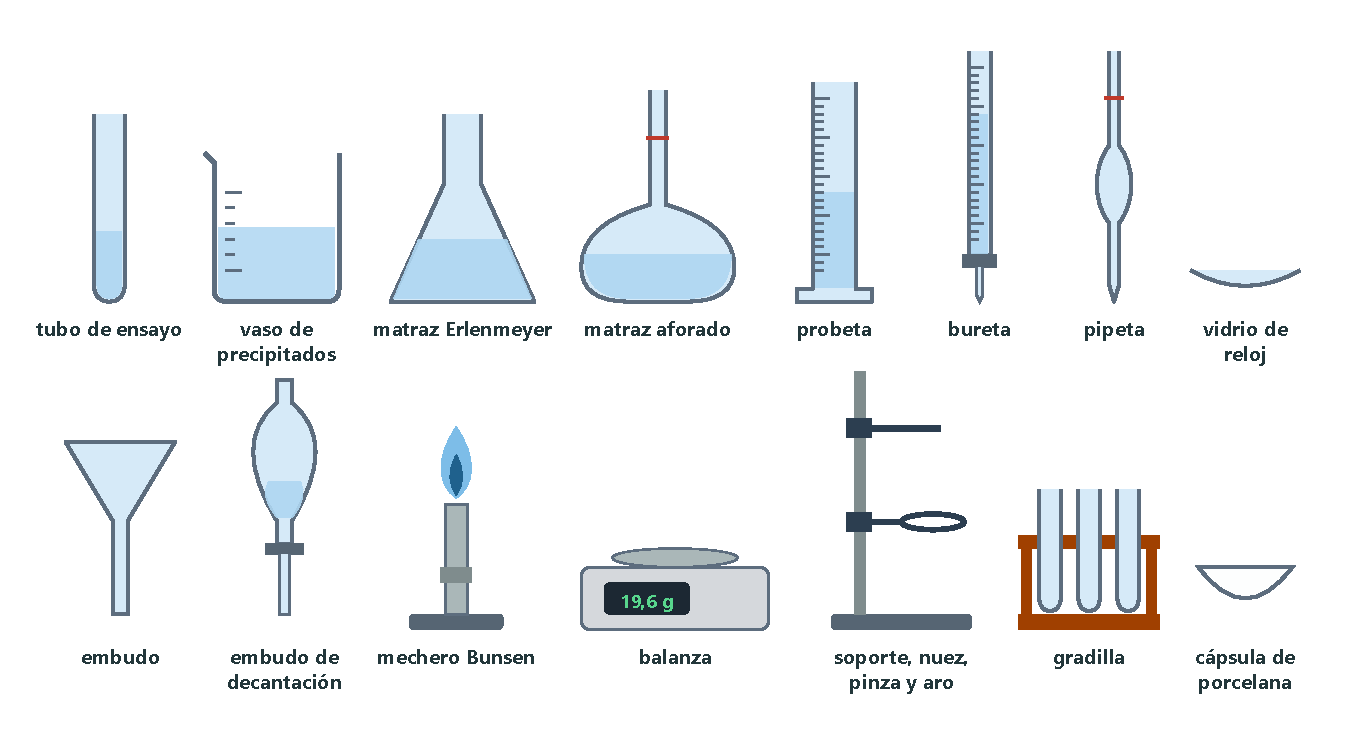
\includegraphics[width=\textwidth]{images/UD1/material_laboratorio}
    \caption{Material de laboratorio de uso frecuente.}
    \label{fig:material_laboratorio}
\end{figure}

Las etiquetas de los productos químicos informan de sus peligros mediante unos \textbf{pictogramas} normalizados: un símbolo negro sobre fondo blanco, dentro de un rombo con borde rojo (figura~\ref{fig:pictogramas}).

\begin{figure}[H]
    \centering
    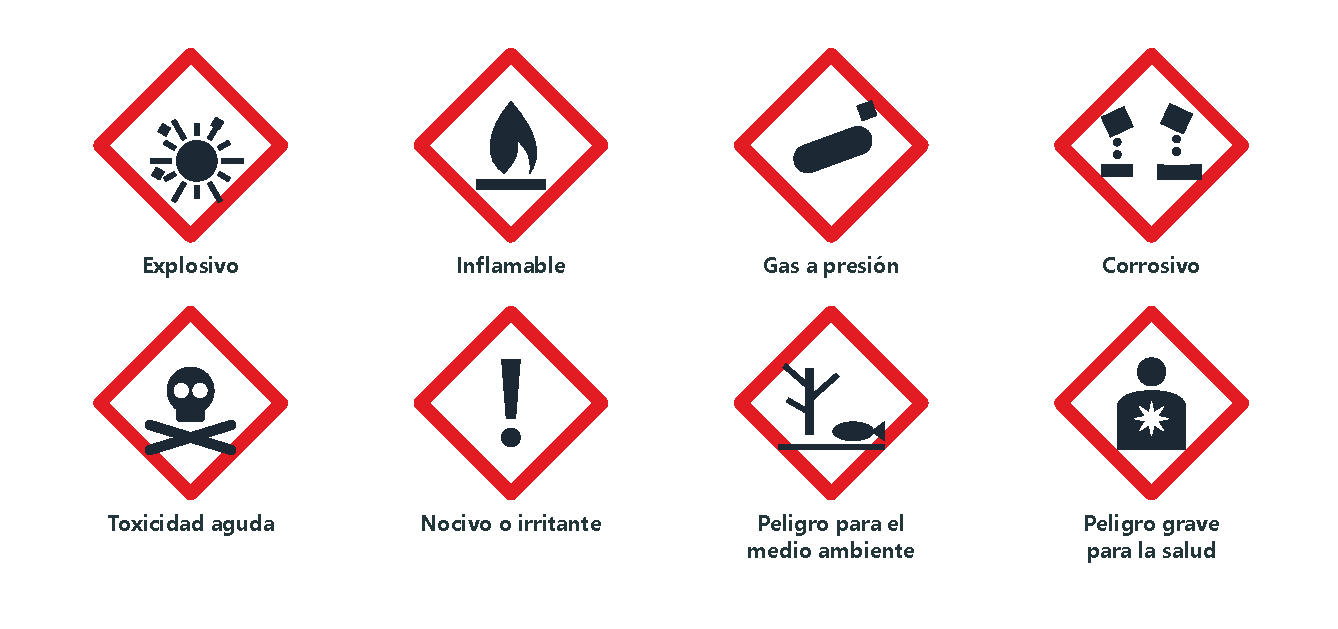
\includegraphics[width=\textwidth]{images/UD1/pictogramas}
    \caption{Pictogramas de peligro de los productos químicos.}
    \label{fig:pictogramas}
\end{figure}

\begin{exercise}
    Busca información sobre los pictogramas de la figura~\ref{fig:pictogramas} y explica qué normas de seguridad reducen el riesgo de cada uno.
    \begin{solu}
        Respuesta abierta. \textcolor{red}{Explosivo}: evitar golpes, fricción y calor. \textcolor{red}{Inflamable}: alejar de llamas y fuentes de calor. \textcolor{red}{Gas a presión}: no calentar las botellas y sujetarlas bien. \textcolor{red}{Corrosivo}: usar guantes y gafas. \textcolor{red}{Toxicidad aguda}: no inhalar, ingerir ni tocar; usar la campana y guantes. \textcolor{red}{Nocivo o irritante}: evitar el contacto con la piel y los ojos. \textcolor{red}{Peligro para el medio ambiente}: no verterlo por el desagüe. \textcolor{red}{Peligro grave para la salud}: protección completa y mínima exposición.
    \end{solu}
\end{exercise}

\begin{exercise}
    Nombra el material de la figura~\ref{fig:material_laboratorio} que usarías para: a) medir un volumen de líquido con precisión; b) preparar \qty{250}{\mL} exactos de una disolución; c) calentar una sustancia; d) separar dos líquidos que no se mezclan; e) medir la masa de un sólido.
    \begin{solu}
        a) Una \textcolor{red}{probeta}, una \textcolor{red}{pipeta} o una \textcolor{red}{bureta}; b) un \textcolor{red}{matraz aforado}; c) un \textcolor{red}{mechero Bunsen} (con un tubo de ensayo o un vaso de precipitados); d) un \textcolor{red}{embudo de decantación}; e) una \textcolor{red}{balanza}.
    \end{solu}
\end{exercise}




%------------------------------------------------


    \chapterimage{images/portada_cabeceras/cabecera_UD2}
    \chapter{El átomo y la Tabla Periódica}

    %! Author = crist
%! Date = 24/10/2026

\spacing{1.3}
%----------------------------------------------------------------------------------------
%	UNIDAD 2: EL ÁTOMO Y LA TABLA PERIÓDICA (4.º ESO)
%   Figuras: images/UD2/*.pdf (fuente HTML en images/UD2/html, SVG en images/UD2/svg)
%----------------------------------------------------------------------------------------

%------------------------------------------------
% Comandos propios de la unidad
%------------------------------------------------
% Configuración electrónica en letra recta: \conf{1s^2~2s^2~2p^6}
\providecommand{\conf}[1]{\(\mathrm{#1}\)}

% Espectros dibujados con TikZ (para los ejercicios)
\pgfdeclarehorizontalshading{arcoiris}{100bp}{%
    rgb(0bp)=(0.45,0,0.55); rgb(18bp)=(0.25,0,1); rgb(32bp)=(0,0.55,1); rgb(42bp)=(0,0.9,0.9);
    rgb(52bp)=(0,0.9,0.2); rgb(65bp)=(1,1,0); rgb(78bp)=(1,0.5,0); rgb(90bp)=(1,0,0); rgb(100bp)=(0.45,0,0)}
% Posiciones de las rayas entre 0 y 1 (0 = violeta, 1 = rojo)
\providecommand{\espectrocontinuo}{%
    \begin{tikzpicture}[x=6cm,y=0.7cm]
        \shade[shading=arcoiris] (0,0) rectangle (1,1);
    \end{tikzpicture}}
\providecommand{\espectroemision}[1]{%
    \begin{tikzpicture}[x=6cm,y=0.7cm]
        \fill[black] (0,0) rectangle (1,1);
        \foreach \p/\c in {#1} {\fill[\c] (\p-0.005,0) rectangle (\p+0.005,1);}
    \end{tikzpicture}}
\providecommand{\espectroabsorcion}[1]{%
    \begin{tikzpicture}[x=6cm,y=0.7cm]
        \shade[shading=arcoiris] (0,0) rectangle (1,1);
        \foreach \p in {#1} {\fill[black] (\p-0.005,0) rectangle (\p+0.005,1);}
    \end{tikzpicture}}

% Mapa conceptual del tema (fuente en images/mapas_conceptuales/html/temas.js)
\begin{figure}[H]
    \centering
    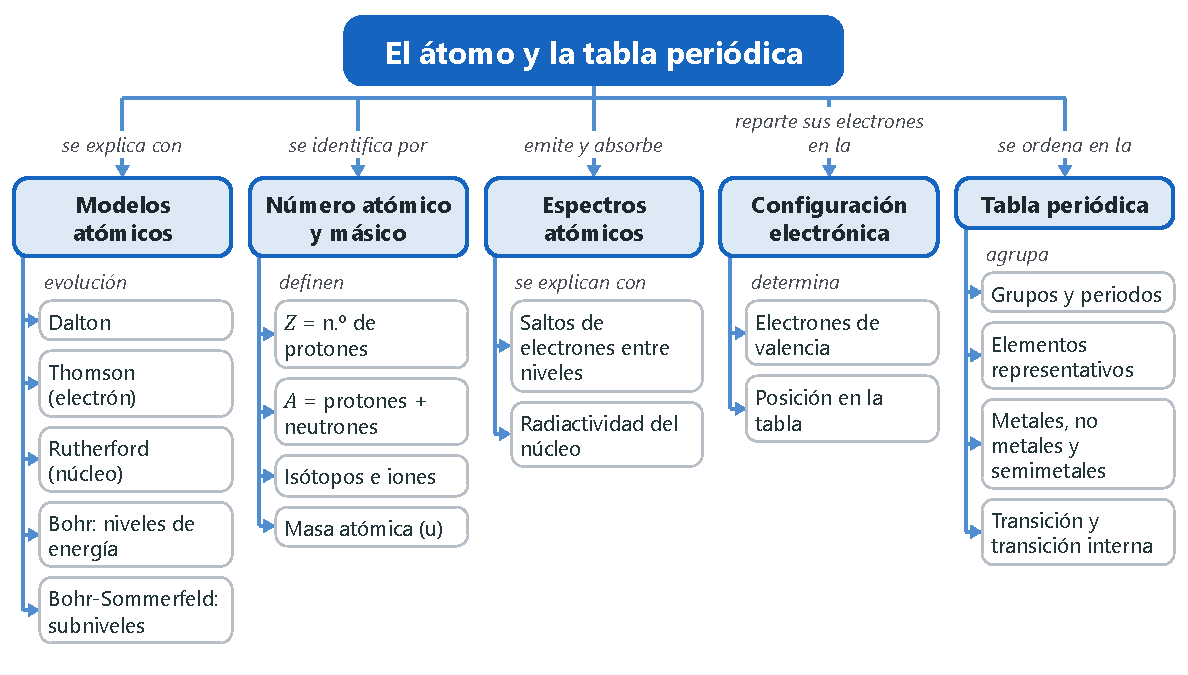
\includegraphics[width=\textwidth]{images/mapas_conceptuales/mapa_UD2}
\end{figure}

%========================================================================================
%\section*{Para empezar: las tierras raras}
%\addcontentsline{toc}{section}{Para empezar: las tierras raras}
%========================================================================================
%
%Con el nombre de \textbf{tierras raras} se conoce a un grupo de \textbf{17 elementos químicos}: los 15 lantanoides, más el escandio y el itrio. Estos dos últimos se incluyen en el grupo porque aparecen en los mismos yacimientos y tienen propiedades químicas, ópticas y magnéticas muy parecidas.
%
%Aunque su nombre sugiere lo contrario, no son tan escasos; lo difícil es encontrarlos concentrados y separarlos unos de otros. Hoy son imprescindibles en telecomunicaciones, electrónica, medicina, nanotecnología, electrodomésticos o en la producción y almacenamiento de energía. Sin ellos no existirían los vehículos eléctricos, los aerogeneradores ni muchas placas solares: nuestra tecnología retrocedería varias décadas.
%
%Un teléfono móvil contiene entre 65 y 70 elementos distintos, y ocho de ellos son tierras raras: gracias a ellos la pantalla tiene colores intensos, los altavoces suenan y el teléfono vibra. En medicina se emplean en resonancias magnéticas, equipos de rayos X, tomografías y en algunas terapias contra el cáncer.
%
%\begin{remark}
%    \textbf{Tierras raras y Objetivos de Desarrollo Sostenible.} Su uso en diagnóstico y tratamiento médico las relaciona con el \textbf{ODS 3} (\emph{Salud y bienestar}); su papel en las «tecnologías limpias» (baterías, aerogeneradores, placas solares) las conecta con el \textbf{ODS 7} (\emph{Energía asequible y no contaminante}). Sin embargo, se extraen en minas a cielo abierto con un elevado coste ambiental.
%\end{remark}
%
%\begin{exercise}
%    Busca en la tabla periódica el nombre, el símbolo y el número atómico de las 17 tierras raras.
%    \begin{solu}
%        Escandio, Sc, 21; itrio, Y, 39; lantano, La, 57; cerio, Ce, 58; praseodimio, Pr, 59; neodimio, Nd, 60; prometio, Pm, 61; samario, Sm, 62; europio, Eu, 63; gadolinio, Gd, 64; terbio, Tb, 65; disprosio, Dy, 66; holmio, Ho, 67; erbio, Er, 68; tulio, Tm, 69; iterbio, Yb, 70; lutecio, Lu, 71.
%    \end{solu}
%\end{exercise}
%
%\begin{exercise}
%    ¿Están todas las tierras raras en el mismo grupo y en el mismo período de la tabla?
%    \begin{solu}
%        No. Los lantanoides están todos en el período 6 (en la fila separada de la parte inferior). El escandio y el itrio están en el mismo grupo (grupo 3), pero en períodos distintos (4 y 5, respectivamente).
%    \end{solu}
%\end{exercise}
%
%\begin{exercise}
%    Explica con tus palabras por qué se afirma que, sin estos elementos, la tecnología retrocedería varias décadas. ¿En qué sectores se usan y qué aplicaciones tienen?
%    \begin{solu}
%        Porque forman parte de casi todos los dispositivos electrónicos y de las tecnologías energéticas actuales: sin ellos no habría transición energética ni tecnología punta. Se usan en telecomunicaciones, electrónica (móviles, ordenadores, tabletas), medicina, energía, electrodomésticos y nanotecnología.
%    \end{solu}
%\end{exercise}
%
%\begin{exercise}
%    Teniendo en cuenta lo que has leído, ¿por qué es tan importante reciclar los móviles y otros aparatos electrónicos? Relaciona tu respuesta con los ODS 3 y 7.
%    \begin{solu}
%        Porque contienen elementos valiosos y difíciles de obtener, cuya extracción tiene un alto coste ambiental. Reciclarlos permite recuperarlos sin abrir nuevas minas. Estos elementos se usan en el diagnóstico y tratamiento de enfermedades (ODS 3) y en las tecnologías limpias de producción de energía (ODS 7).
%    \end{solu}
%\end{exercise}

%========================================================================================
\section{Los primeros modelos atómicos y la radiactividad}
%========================================================================================

Hace unos 2\,400 años, los filósofos griegos \textbf{Leucipo} y \textbf{Demócrito} propusieron que la materia no puede dividirse indefinidamente: tiene que existir una porción mínima e indivisible, a la que llamaron \textbf{átomo}, palabra que significa «\emph{que no se puede dividir}». Era una idea filosófica, sin experimentos que la apoyasen.

\begin{definition}[Modelo científico]
    Un \textbf{modelo} es una representación simplificada de la realidad que intenta explicar los hechos experimentales.
    Es mejor cuantos más hechos explica. Si aparece un descubrimiento que el modelo no puede explicar, el modelo se revisa o se sustituye por otro.
\end{definition}

\begin{figure}[H]
    \centering
    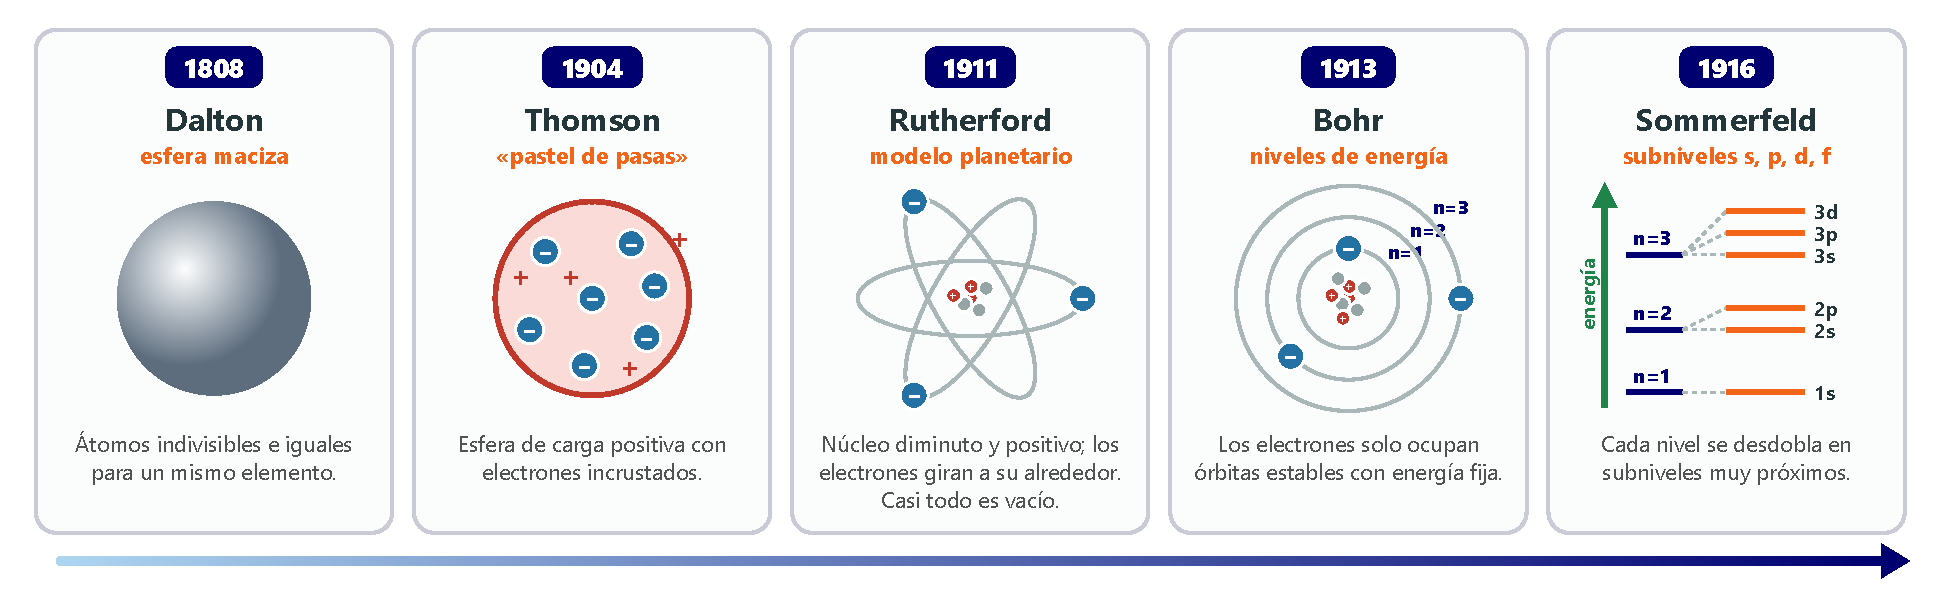
\includegraphics[width=\textwidth]{images/UD2/modelos_atomicos}
    \caption{Evolución de los modelos atómicos que estudiarás en esta unidad.}
    \label{fig:modelos_atomicos}
\end{figure}

\subsection{La teoría atómica de Dalton}

En 1808, el químico inglés \textbf{John Dalton} recuperó la idea de átomo, pero esta vez para explicar resultados experimentales (las leyes de las reacciones químicas). Su \textbf{teoría atómica} se resume en estos postulados:

\begin{enumerate}[label=\numberballblue]
    \item La materia está formada por partículas diminutas, \textbf{indivisibles e inalterables}, llamadas átomos.
    \item Todos los átomos de un mismo elemento son \textbf{iguales} entre sí: tienen la misma masa y las mismas propiedades.
    \item Los átomos de elementos distintos tienen masas y propiedades \textbf{diferentes}.
    \item Los compuestos se forman al unirse átomos de dos o más elementos en una \textbf{proporción de números enteros sencillos}.
\end{enumerate}

\subsection{El átomo es divisible: el electrón y el protón}

El modelo de Dalton fue aceptado durante buena parte del siglo \textsc{xix}. Sin embargo, a finales de ese siglo, los experimentos con \textbf{tubos de descarga} (tubos de vidrio con un gas a muy baja presión sometido a un voltaje muy alto) demostraron que los átomos contienen partículas más pequeñas.

\begin{itemize}
    \item \negsubro{El electrón.} En 1897, \textbf{J.\,J. Thomson} demostró que los \emph{rayos catódicos} que se producen en el tubo son haces de partículas con carga negativa, que salen del electrodo negativo (cátodo) y se dirigen al positivo (ánodo). Stoney las había llamado \textbf{electrones}.
    \item \negsubro{El protón.} En 1886, \textbf{E. Goldstein}, usando un cátodo perforado, observó unos rayos positivos (\emph{rayos canales}) que viajan en sentido contrario, del ánodo al cátodo. La partícula positiva más ligera se obtiene con hidrógeno; Rutherford la llamó \textbf{protón} en 1925.
\end{itemize}

\begin{figure}[H]
    \centering
    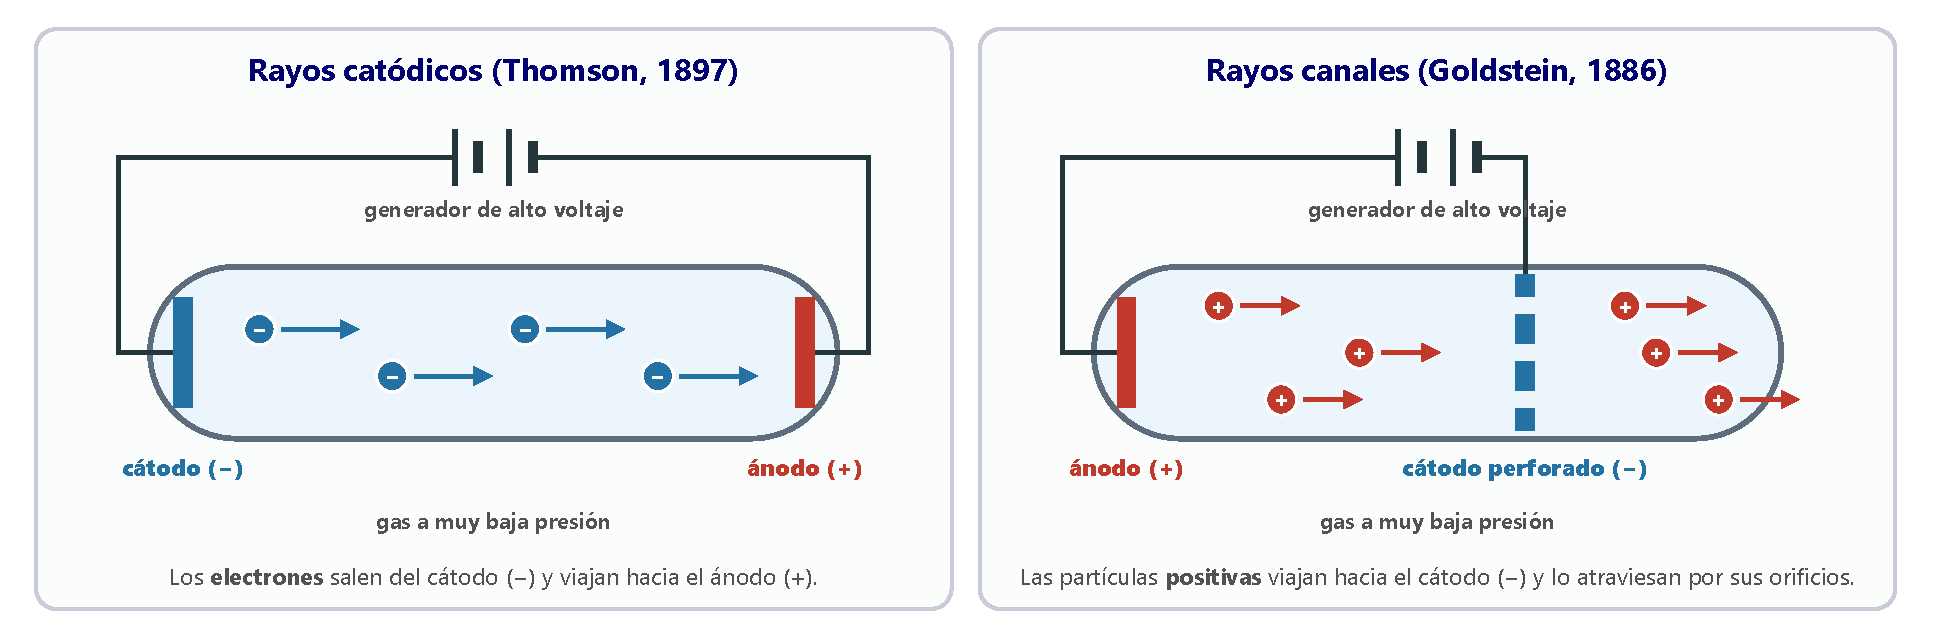
\includegraphics[width=\textwidth]{images/UD2/tubos_descarga}
    \caption{Tubos de descarga: descubrimiento del electrón (izquierda) y del protón (derecha).}
    \label{fig:tubos_descarga}
\end{figure}

\begin{table}[H]
    \centering
    % --- tabla antigua ---
    % \begin{tblr}{colspec={lccc}, hlines, vlines, row{1}={bg=ocre!85, fg=white, font=\bfseries}, column{1}={bg=ocre!15, font=\bfseries}, cell{1}{1}={bg=ocre!85, fg=white}}
        % Partícula & Electrón & Protón & Neutrón \\
        % Carga eléctrica & \qty{-1.602e-19}{\coulomb} & \qty{+1.602e-19}{\coulomb} & sin carga \\
        % Masa & \qty{9.109e-31}{\kg} & \qty{1.673e-27}{\kg} & \qty{1.675e-27}{\kg} \\
        % Descubrimiento & Thomson, 1897 & Goldstein, 1886 & Chadwick, 1932 \\
    % \end{tblr}
    % --- tabla nueva ---
    \begin{tabular}{@{}lccc@{}}
        \toprule
        \textbf{Partícula} & \textbf{Electrón} & \textbf{Protón} & \textbf{Neutrón} \\
        \midrule
        \textbf{Carga eléctrica} & \qty{-1.602e-19}{\coulomb} & \qty{+1.602e-19}{\coulomb} & sin carga \\[3pt]
        \textbf{Masa} & \qty{9.109e-31}{\kg} & \qty{1.673e-27}{\kg} & \qty{1.675e-27}{\kg} \\[3pt]
        \textbf{Descubrimiento} & Thomson, 1897 & Goldstein, 1886 & Chadwick, 1932 \\
        \bottomrule
    \end{tabular}
    \caption{Características de las partículas subatómicas.}
    \label{tab:particulas}
\end{table}

\begin{remark}
    El protón y el electrón tienen cargas \textbf{iguales en valor y de signo contrario}, pero el protón es unas \textbf{1\,836 veces más pesado} que el electrón. El neutrón (que estudiarás más adelante) tiene una masa casi igual a la del protón.
\end{remark}

¿Qué conclusiones se obtienen de estos descubrimientos?
\begin{enumerate}[label=\numberballgreen]
    \item El átomo \textbf{sí es divisible}: contiene partículas subatómicas.
    \item Los electrones tienen \textbf{carga negativa}.
    \item El resto del átomo tiene \textbf{carga positiva} y contiene casi toda la masa.
    \item Como el átomo es eléctricamente neutro, el número de cargas negativas (electrones) es \textbf{igual} al de cargas positivas (protones).
\end{enumerate}

\begin{exercise}
    La carga de un electrón es \qty{-1.6e-19}{\coulomb}. ¿Cuántos electrones hacen falta para reunir una carga total de \qty{-2}{\coulomb}?
    \begin{solu}
        \textcolor{blue}{Dividimos la carga total entre la carga de un electrón:}
        \[ N = \frac{Q}{q_e} = \frac{\qty{-2}{\coulomb}}{\qty{-1.6e-19}{\coulomb}} = \textcolor{red}{\num{1.25e19}\ \text{electrones}} \]
    \end{solu}
\end{exercise}

\begin{exercise}
    ¿Podía explicar la teoría de Dalton la existencia de electrones y protones? Razónalo.
    \begin{solu}
        No. Para Dalton el átomo era indivisible, es decir, no tenía partes. La existencia de partículas más pequeñas que el átomo contradice directamente su primer postulado.
    \end{solu}
\end{exercise}

\subsection{El modelo atómico de Thomson}

Con estos datos, Thomson propuso en 1904 el primer modelo de átomo con partes, conocido como modelo del \textbf{«pastel de pasas»}: el átomo sería una \textbf{esfera de carga positiva} en la que los \textbf{electrones} están incrustados, como las pasas en un bizcocho. La carga positiva total compensa la negativa, de modo que el átomo es neutro (figura~\ref{fig:modelo_thomson}).

\begin{figure}[H]
    \centering
    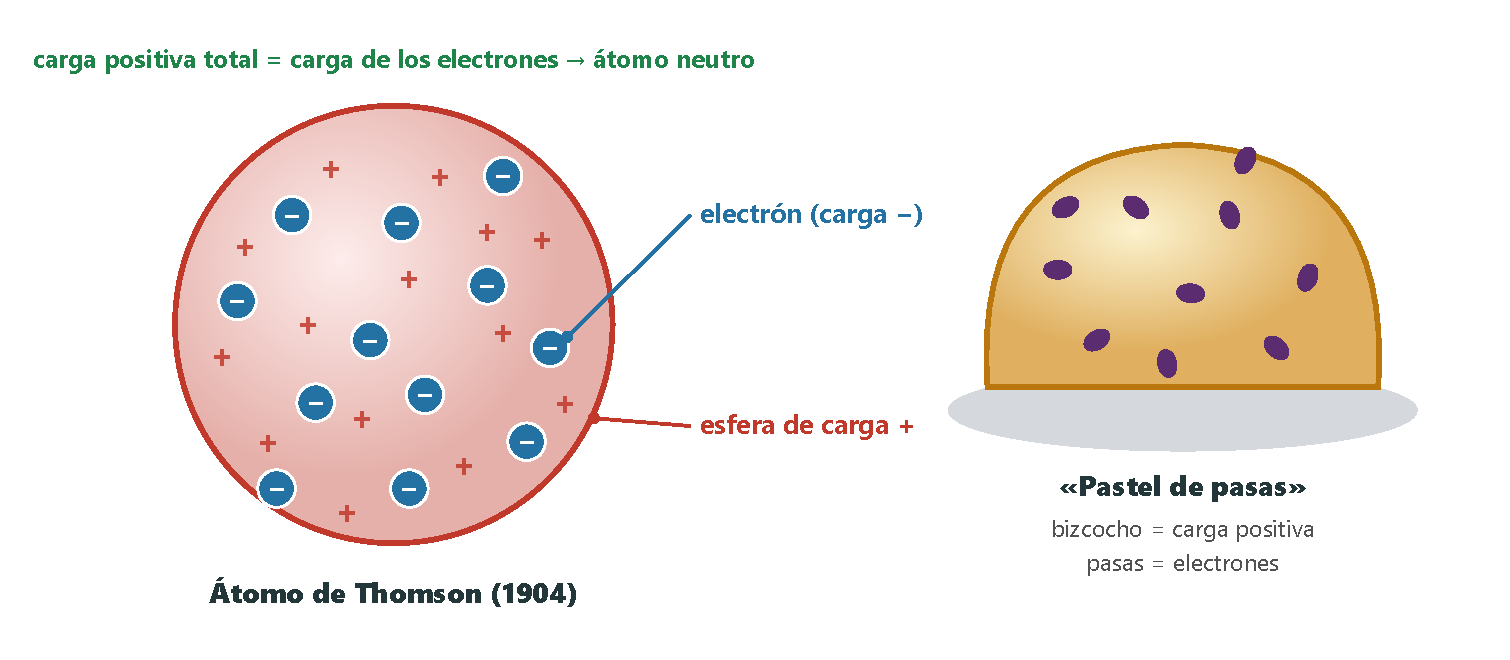
\includegraphics[width=0.9\textwidth]{images/UD2/modelo_thomson}
    \caption{Modelo atómico de Thomson: los electrones están incrustados en una esfera de carga positiva, como las pasas en un bizcocho.}
    \label{fig:modelo_thomson}
\end{figure}

Este modelo se aceptó hasta que nuevos experimentos demostraron que el interior del átomo no podía ser así.

\subsection{El modelo planetario de Rutherford}

\paragraph{El átomo no es un pastel de pasas.} En 1911, \textbf{Ernest Rutherford} y sus colaboradores \textbf{Geiger} y \textbf{Marsden} bombardearon una lámina de oro muy fina con \textbf{partículas alfa} (partículas positivas y rápidas). Una pantalla de sulfuro de zinc colocada alrededor emitía un destello cada vez que recibía una partícula. Observaron que:

\begin{itemize}
    \item La \textbf{inmensa mayoría} de las partículas \textbf{atravesaba} la lámina sin desviarse.
    \item \textbf{Algunas} se \textbf{desviaban} bastante de su trayectoria.
    \item \textbf{Muy pocas} (aproximadamente una de cada 10\,000) \textbf{rebotaban} y volvían hacia la fuente.
\end{itemize}

\begin{figure}[H]
    \centering
    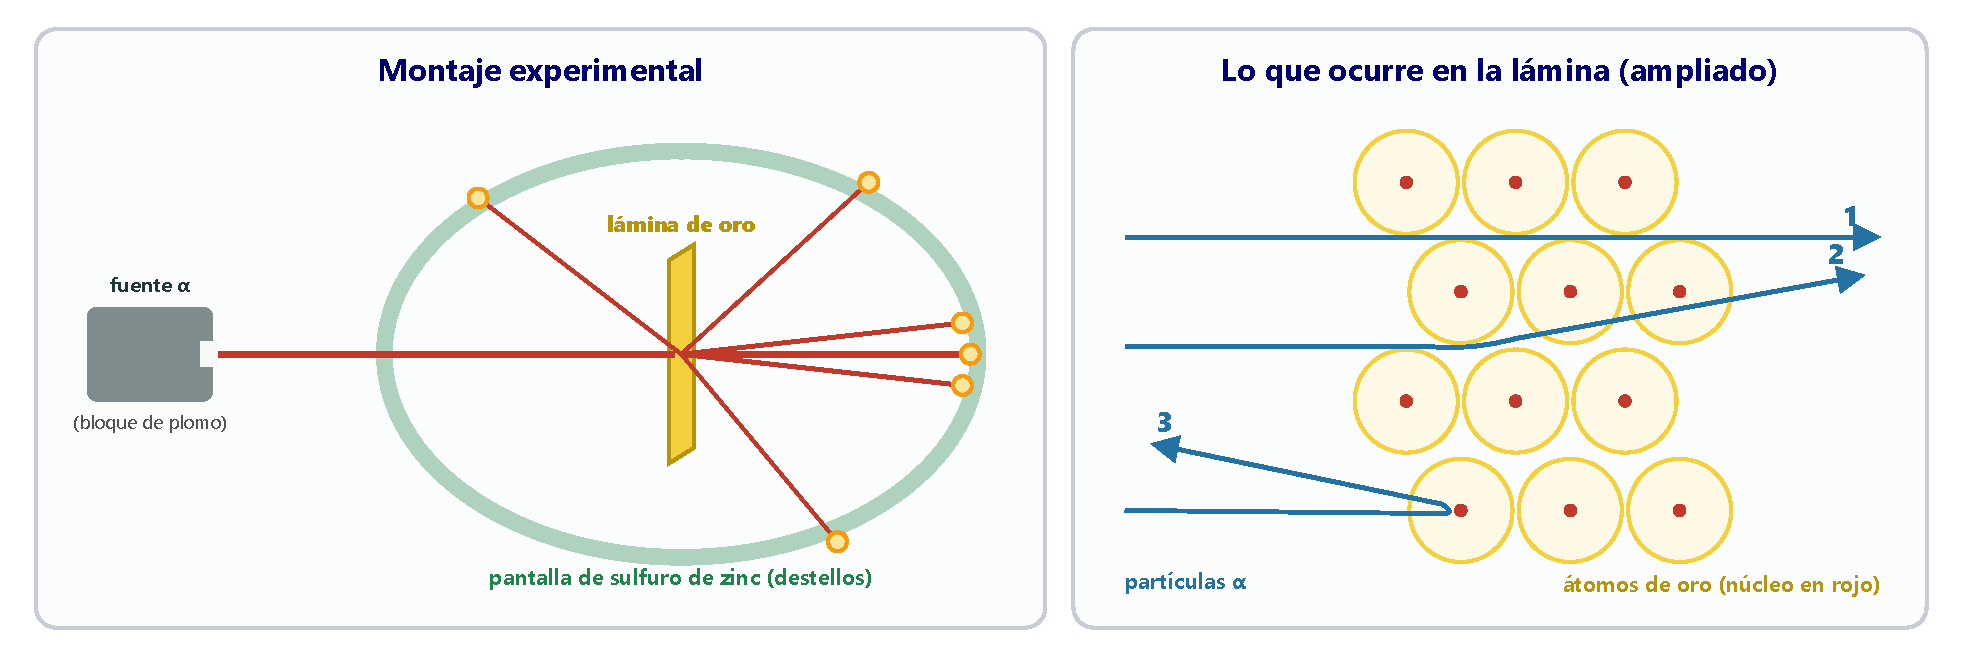
\includegraphics[width=\textwidth]{images/UD2/experimento_rutherford}
    \caption{Experimento de Rutherford, Geiger y Marsden. A la derecha: (1) la partícula pasa lejos de los núcleos y no se desvía; (2) pasa cerca de un núcleo y es repelida; (3) choca de frente con un núcleo y rebota.}
    \label{fig:experimento_rutherford}
\end{figure}

El modelo de Thomson no podía explicar el rebote de algunas partículas: en una esfera positiva «blanda» y uniforme no hay nada lo bastante concentrado para hacerlas volver.

\paragraph{El modelo planetario.} Rutherford propuso entonces un modelo nuevo:
\begin{itemize}
    \item El átomo es, en su mayor parte, \textbf{espacio vacío}.
    \item En el centro hay un \textbf{núcleo} diminuto en el que se concentran \textbf{toda la carga positiva} y \textbf{casi toda la masa} del átomo.
    \item Los \textbf{electrones} giran a gran velocidad alrededor del núcleo, a una distancia muy grande comparada con su tamaño, como los planetas alrededor del Sol. Esta zona se llama \textbf{corteza}.
\end{itemize}

Así se explica el experimento: casi todas las partículas atraviesan el espacio vacío (1); las que pasan cerca de un núcleo son repelidas porque ambos son positivos (2); y las pocas que chocan de frente contra un núcleo rebotan (3).

\paragraph{El descubrimiento del neutrón.} Los protones no bastaban para explicar la masa de los núcleos: el núcleo de helio, por ejemplo, tiene dos protones pero una masa cuatro veces la del hidrógeno. Rutherford supuso que debía existir otra partícula en el núcleo, con masa pero sin carga. En 1932, \textbf{James Chadwick} la descubrió y la llamó \textbf{neutrón}.

\begin{remark}
    \textbf{¡Qué vacío está el átomo!} Si el núcleo de un átomo tuviera el tamaño de una canica colocada en el centro de un campo de fútbol, los electrones estarían girando más allá de las gradas.
\end{remark}

\paragraph{Electrización de la materia y formación de iones.} El modelo de Rutherford explica fenómenos como la electrización. Un cuerpo neutro tiene tantas cargas positivas como negativas. Al frotarlo, puede \textbf{ganar} electrones (y se carga negativamente) o \textbf{perder} electrones (y se carga positivamente). Los protones nunca se mueven: están fijos en el núcleo.

Del mismo modo, un átomo neutro puede ganar o perder electrones y convertirse en un \textbf{ion}:
\begin{itemize}
    \item Si \textbf{pierde} electrones queda con carga positiva: es un \textbf{catión} (por ejemplo, \ch{Na+}).
    \item Si \textbf{gana} electrones queda con carga negativa: es un \textbf{anión} (por ejemplo, \ch{Cl-}).
\end{itemize}

\begin{figure}[H]
    \centering
    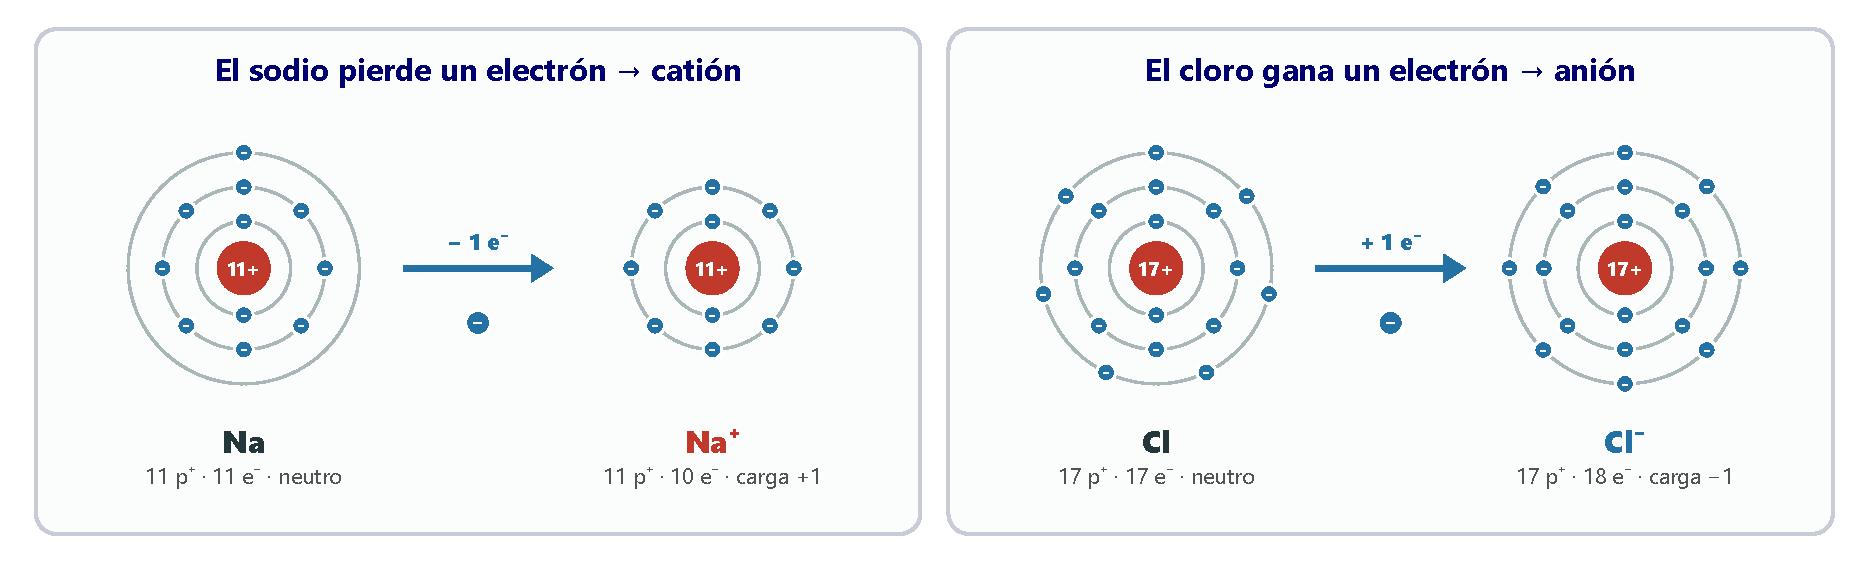
\includegraphics[width=\textwidth]{images/UD2/iones}
    \caption{Formación de un catión y de un anión: solo cambia el número de electrones.}
    \label{fig:iones}
\end{figure}

\subsection{Un fenómeno nuclear: la radiactividad}

En 1896, \textbf{Henri Becquerel} descubrió por casualidad que unas placas fotográficas envueltas en papel se habían velado al guardarlas junto a un mineral de uranio. El mineral emitía algo capaz de atravesar el papel. Marie y Pierre Curie estudiaron el fenómeno, que llamaron \textbf{radiactividad}.

\begin{definition}[Radiactividad]
    Es el fenómeno por el cual los \textbf{núcleos} de algunos átomos emiten \textbf{espontáneamente} partículas y radiaciones, transformándose en núcleos de otros elementos.
\end{definition}

Rutherford comprobó que, al hacer pasar estas emisiones entre dos placas cargadas, se separaban en tres tipos:

\begin{itemize}
    \item \negsubro{Partículas alfa (\(\alpha\)).} Formadas por \textbf{dos protones y dos neutrones} (son núcleos de helio). Tienen carga positiva, por lo que se desvían hacia la placa negativa. Son relativamente lentas y muy poco penetrantes: \textbf{una hoja de papel las detiene}.
    \item \negsubro{Partículas beta (\(\beta\)).} Son \textbf{electrones} muy rápidos. Se desvían mucho hacia la placa positiva y son más penetrantes: atraviesan el papel, pero \textbf{una lámina de aluminio de unos milímetros las detiene}. Se originan en el núcleo cuando un neutrón se transforma en un protón y un electrón, que sale despedido.
    \item \negsubro{Rayos gamma (\(\gamma\)).} No son partículas, sino \textbf{radiación} de mucha energía que viaja a la velocidad de la luz. No se desvían y son los más penetrantes: atraviesan finas capas de metal y los seres vivos, y solo los detienen gruesas capas de \textbf{plomo u hormigón}.
\end{itemize}

\begin{figure}[H]
    \centering
    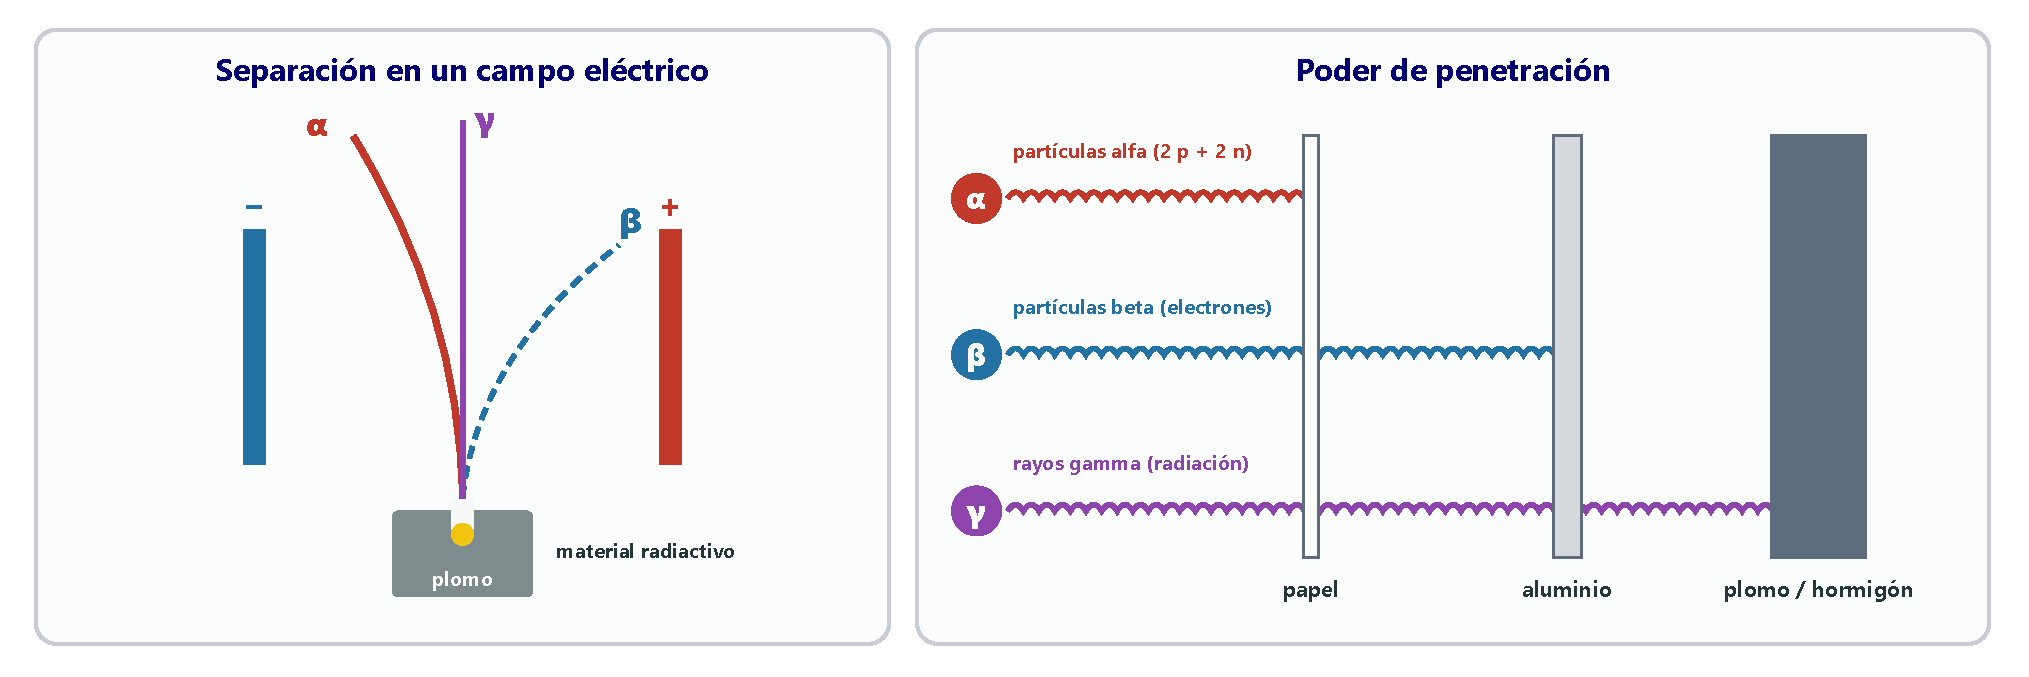
\includegraphics[width=\textwidth]{images/UD2/radiactividad}
    \caption{Comportamiento de las radiaciones \(\alpha\), \(\beta\) y \(\gamma\) en un campo eléctrico y su poder de penetración.}
    \label{fig:radiactividad}
\end{figure}

\begin{exercise}
    Investiga y describe tres aplicaciones de la radiactividad en medicina y otras dos en otros campos (industria, arqueología, energía…).
    \begin{solu}
        Respuesta libre. Por ejemplo: en medicina, la radioterapia contra el cáncer, los contrastes radiactivos para diagnóstico (gammagrafías, PET) y la esterilización de material quirúrgico. En otros campos: la datación por carbono-14 en arqueología, el control de soldaduras en la industria o la producción de energía en las centrales nucleares.
    \end{solu}
\end{exercise}

\begin{exercise}
    ¿Qué significaba originalmente la palabra «átomo»? ¿Quiénes la utilizaron por primera vez?
    \begin{solu}
        Significa «indivisible», «que no se puede dividir». La utilizaron por primera vez los filósofos griegos Leucipo y Demócrito, en el siglo \textsc{v}-\textsc{iv} a.\,C.
    \end{solu}
\end{exercise}

\begin{exercise}
    Escribe con tus propias palabras los postulados de la teoría atómica de Dalton. ¿Cuál de ellos tuvo que abandonarse primero?
    \begin{solu}
        Respuesta libre (ver los cuatro postulados del apartado 1.1). El primero que tuvo que abandonarse fue el de que los átomos son indivisibles, tras el descubrimiento del electrón y del protón.
    \end{solu}
\end{exercise}

\begin{exercise}
    ¿En qué experimentos se descubrieron el electrón y el protón? ¿Por qué fue tan importante este descubrimiento para la teoría atómica?
    \begin{solu}
        En los experimentos con tubos de descarga de gases (rayos catódicos y rayos canales). Fue importante porque demostró que el átomo es divisible: está formado por partículas más pequeñas con carga eléctrica.
    \end{solu}
\end{exercise}

\begin{exercise}
    ¿Cómo explicaba el modelo de Thomson que el átomo tuviera cargas positivas y negativas y que, aun así, fuera neutro?
    \begin{solu}
        Con el modelo del «pastel de pasas»: una esfera de carga positiva repartida uniformemente con los electrones incrustados en ella. La carga positiva de la esfera es igual a la suma de las cargas negativas de los electrones, por lo que el conjunto es neutro.
    \end{solu}
\end{exercise}

\begin{exercise}
    Indica cuáles de estas afirmaciones son falsas y corrígelas:
    \begin{enumerate}[label=\alph*)]
        \item En un átomo neutro hay tantos electrones como protones.
        \item El neutrón no tiene carga y su masa es menor que la del protón.
        \item Casi toda la masa del átomo se debe a los protones y los neutrones.
        \item El electrón es más pesado que el protón.
        \item El neutrón fue la última de las tres partículas en descubrirse.
        \item El protón y el electrón tienen cargas del mismo valor, pero de signo opuesto.
        \item Protones y neutrones se encuentran en el núcleo.
    \end{enumerate}
    \begin{solu}
        \begin{enumerate}[label=\alph*)]
            \item Verdadera.
            \item \textcolor{red}{Falsa.} El neutrón no tiene carga y su masa es \textbf{ligeramente mayor} que la del protón.
            \item Verdadera.
            \item \textcolor{red}{Falsa.} El protón es unas 1\,836 veces \textbf{más pesado} que el electrón.
            \item Verdadera (Chadwick, 1932).
            \item Verdadera.
            \item Verdadera.
        \end{enumerate}
    \end{solu}
\end{exercise}

\begin{exercise}
    Completa el texto sobre el modelo de Rutherford con las palabras: \emph{electrones, protones, neutrones, núcleo}.

    «Según Rutherford, el átomo es fundamentalmente un espacio vacío con un \rule{1.5cm}{0.4pt} central donde se concentra casi toda su masa, que se debe a los \rule{1.5cm}{0.4pt} y los \rule{1.5cm}{0.4pt}. La carga positiva también está en el \rule{1.5cm}{0.4pt}. Los \rule{1.5cm}{0.4pt} giran a gran velocidad a su alrededor y muy alejados de él.»
    \begin{solu}
        «\ldots con un \textcolor{red}{núcleo} central donde se concentra casi toda su masa, que se debe a los \textcolor{red}{protones} y los \textcolor{red}{neutrones}. La carga positiva también está en el \textcolor{red}{núcleo}. Los \textcolor{red}{electrones} giran a gran velocidad a su alrededor\ldots»
    \end{solu}
\end{exercise}

\begin{exercise}
    Sobre la radiactividad:
    \begin{enumerate}[label=\alph*)]
        \item ¿Qué tipos de partículas y radiaciones emiten las sustancias radiactivas?
        \item Describe brevemente las características de cada una.
        \item Si la radiactividad tiene lugar en el núcleo, ¿cómo es posible que se emitan electrones, si en el núcleo no hay electrones?
    \end{enumerate}
    \begin{solu}
        \begin{enumerate}[label=\alph*)]
            \item Partículas alfa, partículas beta y rayos gamma.
            \item Alfa: 2 protones y 2 neutrones, carga positiva, poco penetrantes (las detiene el papel). Beta: electrones rápidos, más penetrantes (las detiene una lámina de aluminio). Gamma: radiación de alta energía sin carga, muy penetrante (la detienen el plomo o el hormigón).
            \item Porque en el núcleo un neutrón se transforma en un protón y un electrón; el protón se queda en el núcleo y el electrón sale despedido como partícula beta.
        \end{enumerate}
    \end{solu}
\end{exercise}

\begin{exercise}
    Utiliza el modelo de Rutherford para explicar, con ayuda de un dibujo:
    \begin{enumerate}[label=\alph*)]
        \item Por qué una varilla de vidrio se carga al frotarla con un paño.
        \item Cómo se forman un ion positivo y un ion negativo.
    \end{enumerate}
    \begin{solu}
        \begin{enumerate}[label=\alph*)]
            \item Al frotar, algunos electrones pasan del vidrio al paño. El vidrio queda con menos electrones que protones (carga positiva) y el paño con más electrones que protones (carga negativa). Los protones no se mueven.
            \item Un átomo neutro que pierde electrones queda con más protones que electrones: catión (positivo). Si gana electrones, queda con más electrones que protones: anión (negativo). Ver la figura \ref{fig:iones}.
        \end{enumerate}
    \end{solu}
\end{exercise}

%========================================================================================
\section{¿Cómo identificamos los átomos de cada elemento?}
%========================================================================================

Cada átomo tiene una especie de «tarjeta de identidad». Lo que distingue a un átomo de calcio de uno de oxígeno o de hierro es el \textbf{número de protones} de su núcleo, que es siempre el mismo para todos los átomos de un elemento.

\subsection{El número atómico}

\begin{definition}[Número atómico, \(Z\)]
    Es el \textbf{número de protones} que hay en el núcleo de un átomo. Es un número entero y caracteriza al elemento: todos los átomos de un mismo elemento tienen el mismo \(Z\), y dos elementos distintos nunca tienen el mismo.
\end{definition}

Se escribe como subíndice a la izquierda del símbolo: \ch{_{11}Na}, \ch{_{8}O}. En un \textbf{átomo neutro}, el número de electrones es igual al de protones, así que \(Z\) también indica cuántos electrones tiene.

\subsection{El número másico}

\begin{definition}[Número másico, \(A\)]
    Es la \textbf{suma del número de protones y de neutrones} del núcleo. También es un número entero y se escribe como superíndice a la izquierda del símbolo: \ch{^{23}Na}, \ch{^{16}O}.
\end{definition}

\begin{figure}[H]
    \centering
    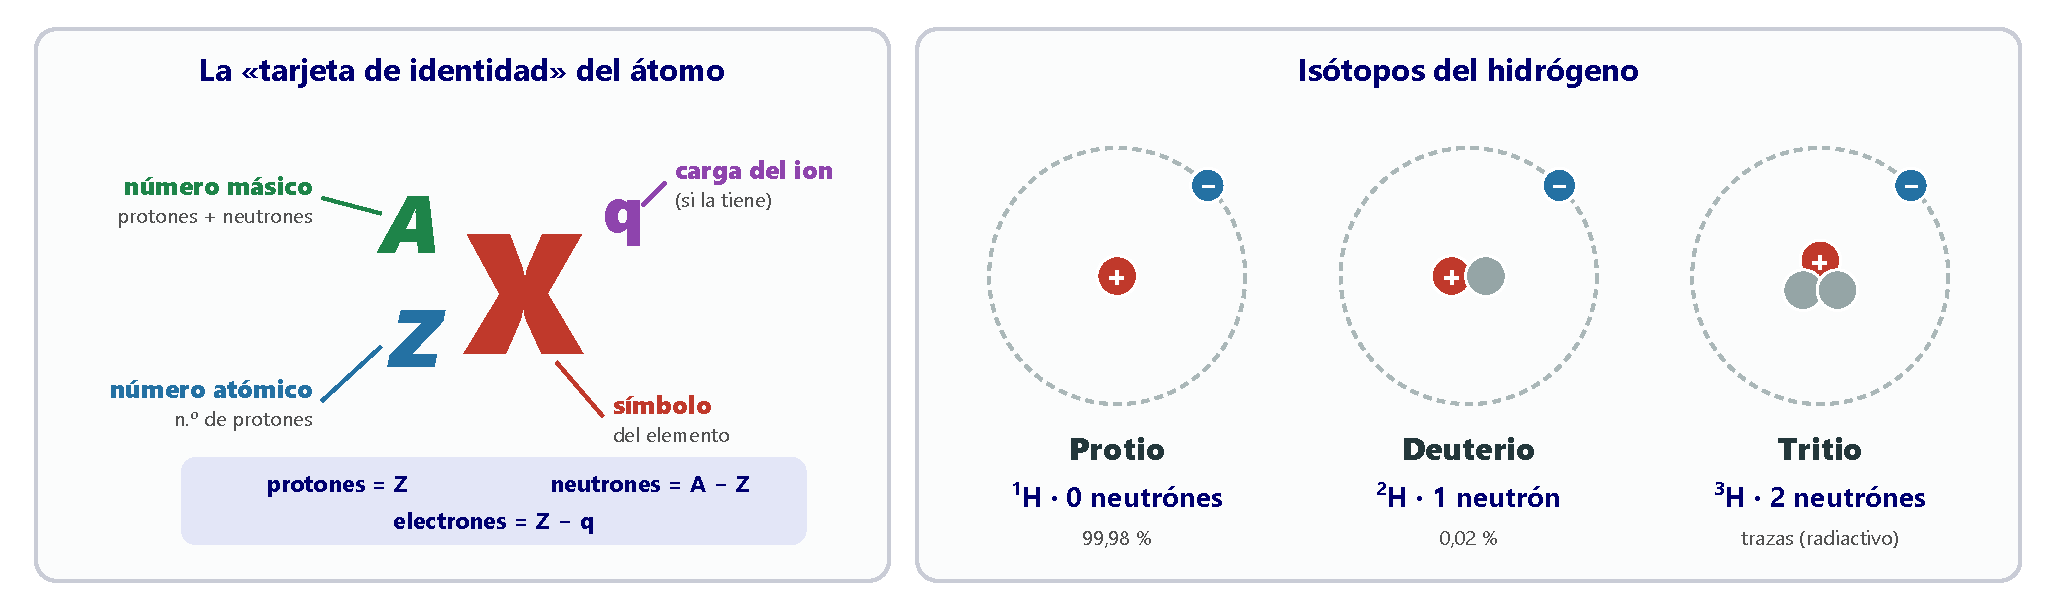
\includegraphics[width=\textwidth]{images/UD2/notacion_isotopos}
    \caption{Notación completa de un átomo o ion y los tres isótopos del hidrógeno.}
    \label{fig:notacion}
\end{figure}

A partir de \(Z\), \(A\) y la carga \(q\) del ion podemos contar todas las partículas:
\begin{centeredequation*}
    \text{protones} = Z \qquad \text{neutrones} = A - Z \qquad \text{electrones} = Z - q
\end{centeredequation*}

\begin{definition}[Isótopos]
    Son átomos de un mismo elemento que tienen el \textbf{mismo número atómico} (mismos protones), pero \textbf{distinto número másico}, porque tienen distinto número de neutrones.
\end{definition}

El número atómico de un elemento solo tiene un valor, pero el número másico puede tener varios, uno por cada isótopo. Por ejemplo, el hidrógeno tiene tres isótopos: protio (\ch{^1H}), deuterio (\ch{^2H}) y tritio (\ch{^3H}).

\begin{remark}
    \textbf{Radioisótopos.} Algunos isótopos tienen núcleos inestables y son radiactivos: se llaman \textbf{radioisótopos}. Por ejemplo, el carbono-14 (\ch{^{14}C}) es un isótopo radiactivo del carbono-12 (\ch{^{12}C}); se usa para datar restos arqueológicos.
\end{remark}

\begin{example}
    \textbf{Electrones de un catión y de un anión.}
    \begin{itemize}
        \item El sodio tiene \(Z = 11\). El átomo neutro tiene 11 protones y 11 electrones. Si pierde un electrón se convierte en el catión \ch{Na+}: sigue teniendo \textbf{11 protones}, pero ahora tiene \textbf{10 electrones}.
        \item El cloro tiene \(Z = 17\). Si un átomo neutro (17 protones, 17 electrones) gana un electrón, se forma el anión \ch{Cl-}: \textbf{17 protones} y \textbf{18 electrones}.
    \end{itemize}
\end{example}

\begin{exercise}
    ¿Es cierta esta frase? Justifica la respuesta: «Un catión y un anión tienen el mismo número de protones y de electrones que el átomo neutro del que proceden».
    \begin{solu}
        \textcolor{red}{Es falsa.} Los iones tienen el mismo número de \textbf{protones} que el átomo neutro, pero distinto número de \textbf{electrones}: el catión tiene menos y el anión tiene más.
    \end{solu}
\end{exercise}

\begin{exercise}
    El cloro tiene dos isótopos naturales, \ch{^{35}_{17}Cl} y \ch{^{37}_{17}Cl}. ¿Cuántos protones, neutrones y electrones tiene un átomo neutro de cloro-37?
    \begin{solu}
        \textcolor{blue}{Protones: \(Z = 17\). Electrones: 17 (es neutro). Neutrones: \(A - Z = 37 - 17\).}

        \textcolor{red}{17 protones, 20 neutrones y 17 electrones.}
    \end{solu}
\end{exercise}

\begin{exercise}
    Calcula el número de protones, neutrones y electrones de estas especies:
    \begin{multicols}{4}
        \begin{enumerate}[label=\alph*)]
            \item \ch{^{79}_{35}Br-}
            \item \ch{^{32}_{16}S^{2-}}
            \item \ch{^{27}_{13}Al^{3+}}
            \item \ch{^{207}_{82}Pb^{4+}}
        \end{enumerate}
    \end{multicols}
    \begin{solu}
        \begin{enumerate}[label=\alph*)]
            \item \ch{^{79}_{35}Br-}: 35 protones, \(79 - 35 = 44\) neutrones, \(35 + 1 = 36\) electrones.
            \item \ch{^{32}_{16}S^{2-}}: 16 protones, 16 neutrones, 18 electrones.
            \item \ch{^{27}_{13}Al^{3+}}: 13 protones, 14 neutrones, 10 electrones.
            \item \ch{^{207}_{82}Pb^{4+}}: 82 protones, 125 neutrones, 78 electrones.
        \end{enumerate}
    \end{solu}
\end{exercise}

\begin{exercise}
    Explica la diferencia entre número atómico y número másico. ¿Por qué los dos son siempre números enteros? ¿Podrían ser decimales?
    \begin{solu}
        El número atómico es el número de protones; el número másico es la suma de protones y neutrones. Son enteros porque cuentan partículas y no existen «trozos» de protón o de neutrón. Por tanto, nunca pueden ser decimales.
    \end{solu}
\end{exercise}

\begin{exercise}
    ¿Cómo se llama el número de protones de un átomo? ¿Pueden dos átomos de elementos distintos tener el mismo número de protones?
    \begin{solu}
        Se llama número atómico. No: si dos átomos tienen el mismo número de protones, son del mismo elemento.
    \end{solu}
\end{exercise}

\begin{exercise}
    ¿Qué es el número másico? ¿Pueden dos átomos de un mismo elemento tener distinto número másico? ¿Cómo se llaman?
    \begin{solu}
        Es la suma de protones y neutrones del núcleo. Sí: tienen los mismos protones pero distinto número de neutrones. Se llaman isótopos.
    \end{solu}
\end{exercise}

\begin{exercise}
    Copia y completa la tabla en tu cuaderno:
    \begin{center}
        % --- tabla antigua ---
        % \begin{tblr}{colspec={cccc}, hlines, vlines, row{1}={bg=ocre!85, fg=white, font=\bfseries}}
            % Átomo & Protones & Electrones & Neutrones \\
            % \ch{^{107}_{47}Ag} & & & \\
            % \ch{^{206}_{82}Pb} & & & \\
            % \ch{^{133}_{55}Cs} & & & \\
            % \ch{^{71}_{31}Ga} & & & \\
        % \end{tblr}
        % --- tabla nueva ---
        \begin{tabular}{@{}cccc@{}}
            \toprule
            \textbf{Átomo} & \textbf{Protones} & \textbf{Electrones} & \textbf{Neutrones} \\
            \midrule
            \ch{^{107}_{47}Ag} &  &  &  \\[3pt]
            \ch{^{206}_{82}Pb} &  &  &  \\[3pt]
            \ch{^{133}_{55}Cs} &  &  &  \\[3pt]
            \ch{^{71}_{31}Ga} &  &  &  \\
            \bottomrule
        \end{tabular}
    \end{center}
    \begin{solu}
        \begin{center}
            % --- tabla antigua ---
            % \begin{tblr}{colspec={cccc}, hlines, vlines, row{1}={font=\bfseries}}
                % Átomo & Protones & Electrones & Neutrones \\
                % \ch{^{107}_{47}Ag} & 47 & 47 & 60 \\
                % \ch{^{206}_{82}Pb} & 82 & 82 & 124 \\
                % \ch{^{133}_{55}Cs} & 55 & 55 & 78 \\
                % \ch{^{71}_{31}Ga} & 31 & 31 & 40 \\
            % \end{tblr}
            % --- tabla nueva ---
            \begin{tabular}{@{}cccc@{}}
                \toprule
                \textbf{Átomo} & \textbf{Protones} & \textbf{Electrones} & \textbf{Neutrones} \\
                \midrule
                \ch{^{107}_{47}Ag} & 47 & 47 & 60 \\[3pt]
                \ch{^{206}_{82}Pb} & 82 & 82 & 124 \\[3pt]
                \ch{^{133}_{55}Cs} & 55 & 55 & 78 \\[3pt]
                \ch{^{71}_{31}Ga} & 31 & 31 & 40 \\
                \bottomrule
            \end{tabular}
        \end{center}
    \end{solu}
\end{exercise}

\begin{exercise}
    Completa la tabla para estos iones:
    \begin{center}
        % --- tabla antigua ---
        % \begin{tblr}{colspec={cccc}, hlines, vlines, row{1}={bg=ocre!85, fg=white, font=\bfseries}}
            % Ion & Protones & Electrones & Neutrones \\
            % \ch{^{4}_{2}He^{2+}} & & & \\
            % \ch{^{16}_{8}O^{2-}} & & & \\
            % \ch{^{23}_{11}Na+} & & & \\
            % \ch{^{81}_{35}Br-} & & & \\
            % \ch{^{24}_{12}Mg^{2+}} & & & \\
            % \ch{^{106}_{46}Pd^{4+}} & & & \\
            % \ch{^{75}_{33}As^{3-}} & & & \\
        % \end{tblr}
        % --- tabla nueva ---
        \begin{tabular}{@{}cccc@{}}
            \toprule
            \textbf{Ion} & \textbf{Protones} & \textbf{Electrones} & \textbf{Neutrones} \\
            \midrule
            \ch{^{4}_{2}He^{2+}} &  &  &  \\[3pt]
            \ch{^{16}_{8}O^{2-}} &  &  &  \\[3pt]
            \ch{^{23}_{11}Na+} &  &  &  \\[3pt]
            \ch{^{81}_{35}Br-} &  &  &  \\[3pt]
            \ch{^{24}_{12}Mg^{2+}} &  &  &  \\[3pt]
            \ch{^{106}_{46}Pd^{4+}} &  &  &  \\[3pt]
            \ch{^{75}_{33}As^{3-}} &  &  &  \\
            \bottomrule
        \end{tabular}
    \end{center}
    \begin{solu}
        \begin{center}
            % --- tabla antigua ---
            % \begin{tblr}{colspec={cccc}, hlines, vlines, row{1}={font=\bfseries}}
                % Ion & Protones & Electrones & Neutrones \\
                % \ch{^{4}_{2}He^{2+}} & 2 & 0 & 2 \\
                % \ch{^{16}_{8}O^{2-}} & 8 & 10 & 8 \\
                % \ch{^{23}_{11}Na+} & 11 & 10 & 12 \\
                % \ch{^{81}_{35}Br-} & 35 & 36 & 46 \\
                % \ch{^{24}_{12}Mg^{2+}} & 12 & 10 & 12 \\
                % \ch{^{106}_{46}Pd^{4+}} & 46 & 42 & 60 \\
                % \ch{^{75}_{33}As^{3-}} & 33 & 36 & 42 \\
            % \end{tblr}
            % --- tabla nueva ---
            \begin{tabular}{@{}cccc@{}}
                \toprule
                \textbf{Ion} & \textbf{Protones} & \textbf{Electrones} & \textbf{Neutrones} \\
                \midrule
                \ch{^{4}_{2}He^{2+}} & 2 & 0 & 2 \\[3pt]
                \ch{^{16}_{8}O^{2-}} & 8 & 10 & 8 \\[3pt]
                \ch{^{23}_{11}Na+} & 11 & 10 & 12 \\[3pt]
                \ch{^{81}_{35}Br-} & 35 & 36 & 46 \\[3pt]
                \ch{^{24}_{12}Mg^{2+}} & 12 & 10 & 12 \\[3pt]
                \ch{^{106}_{46}Pd^{4+}} & 46 & 42 & 60 \\[3pt]
                \ch{^{75}_{33}As^{3-}} & 33 & 36 & 42 \\
                \bottomrule
            \end{tabular}
        \end{center}
    \end{solu}
\end{exercise}

\begin{exercise}
    Observa estos átomos imaginarios (las letras no son símbolos reales):
    \[ \ch{^{50}_{25}A} \quad \ch{^{39}_{19}C} \quad \ch{^{52}_{25}E} \quad \ch{^{102}_{49}G} \quad \ch{^{10}_{5}I} \quad \ch{^{29}_{14}B} \quad \ch{^{110}_{51}D} \quad \ch{^{40}_{19}F} \quad \ch{^{28}_{14}H} \quad \ch{^{51}_{25}J} \]
    \begin{enumerate}[label=\alph*)]
        \item Agrupa los que sean isótopos entre sí.
        \item Indica el número de protones y de neutrones de cada uno de esos isótopos.
        \item ¿En qué se diferencian los isótopos de un mismo grupo?
    \end{enumerate}
    \begin{solu}
        \begin{enumerate}[label=\alph*)]
            \item Son isótopos los que tienen el mismo \(Z\): A, E y J (\(Z = 25\)); B y H (\(Z = 14\)); C y F (\(Z = 19\)).
            \item A, E y J: 25 protones y 25, 27 y 26 neutrones, respectivamente. B y H: 14 protones y 15 y 14 neutrones. C y F: 19 protones y 20 y 21 neutrones.
            \item En el número de neutrones y, por tanto, en el número másico.
        \end{enumerate}
    \end{solu}
\end{exercise}

%========================================================================================
\section{¿Cómo se mide la masa de un átomo? La masa atómica}
%========================================================================================

Un átomo de carbono tiene una masa de unos \qty{2e-26}{\kg}. El kilogramo es una unidad enorme para medir algo tan pequeño, así que los químicos utilizan una unidad mucho más adecuada.

\begin{definition}[Unidad de masa atómica, u]
    Es la \textbf{doceava parte} de la masa de un átomo de carbono-12 (\ch{^{12}C}). Equivale aproximadamente a \qty{1.66e-27}{\kg}.
\end{definition}

\begin{figure}[H]
    \centering
    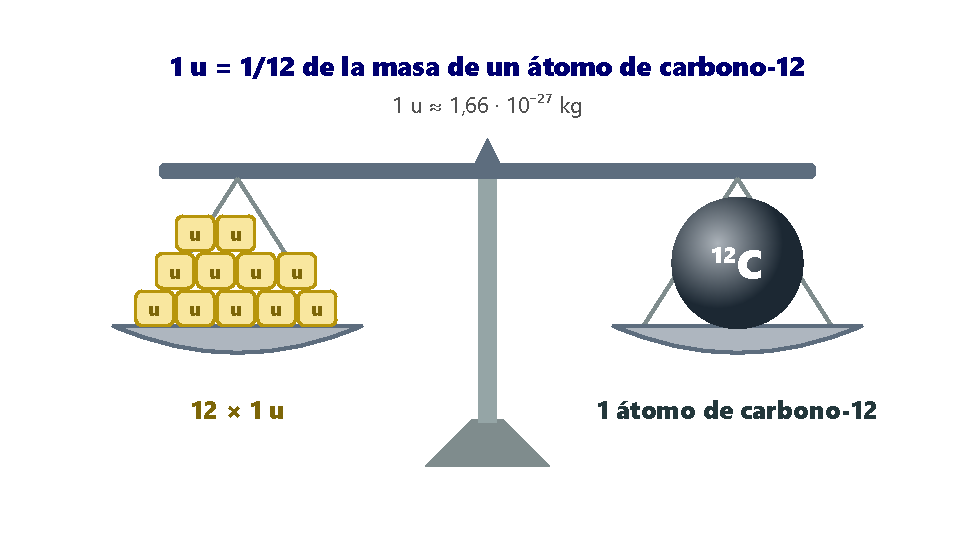
\includegraphics[width=0.6\textwidth]{images/UD2/masa_atomica_balanza}
    \caption{Hacen falta 12 unidades de masa atómica para «equilibrar» un átomo de carbono-12: su masa atómica es 12.}
    \label{fig:balanza}
\end{figure}

\begin{definition}[Masa atómica relativa, \(A_r\)]
    Es la masa de un átomo comparada con la doceava parte de la masa del átomo de carbono-12. Es una magnitud \textbf{adimensional} (no tiene unidades). Se le suele llamar simplemente \textbf{masa atómica}.
\end{definition}

Decir que la masa atómica relativa del oxígeno es 16 significa que un átomo de oxígeno tiene 16 veces más masa que la doceava parte de un átomo de carbono-12.

\subsection{¿Cómo se calcula la masa atómica de un elemento?}

\begin{itemize}
    \item Si el elemento solo tiene \textbf{un isótopo natural} (es \textbf{monoisotópico}), su masa atómica coincide con la de ese isótopo. Por ejemplo, todo el sodio natural es Na-23, así que su masa atómica es 23.
    \item Si el elemento tiene \textbf{varios isótopos}, su masa atómica es la \textbf{media ponderada} de las masas de sus isótopos según su abundancia. Por eso casi nunca es un número entero:
\end{itemize}

\begin{centeredequation}
    A_r = m_1 \cdot \frac{\%_1}{100} + m_2 \cdot \frac{\%_2}{100} + \dots
\end{centeredequation}

donde \(m_1\), \(m_2\)\ldots{} son las masas atómicas relativas de cada isótopo y \(\%_1\), \(\%_2\)\ldots{} sus abundancias. Si no se indica otra cosa, se puede tomar como masa de cada isótopo su número másico.

\begin{example}
    \textbf{Masa atómica del oxígeno.} El oxígeno natural está formado por tres isótopos: oxígeno-16 (\qty{99.759}{\percent}), oxígeno-17 (\qty{0.037}{\percent}) y oxígeno-18 (\qty{0.204}{\percent}). Calcula su masa atómica relativa.

    \textcolor{blue}{Multiplicamos la masa de cada isótopo por su abundancia y sumamos:}
    \[ A_r(\ch{O}) = \frac{16 \cdot \num{99.759} + 17 \cdot \num{0.037} + 18 \cdot \num{0.204}}{100} = \textcolor{red}{\num{16.004}} \]
\end{example}

\begin{exercise}
    Un elemento imaginario está formado por dos isótopos, X-63 y X-65. Si el \qty{60}{\percent} de sus átomos son del primero, ¿cuál es su masa atómica relativa?
    \begin{solu}
        \[ A_r = 63 \cdot \frac{60}{100} + 65 \cdot \frac{40}{100} = \num{37.8} + 26 = \textcolor{red}{\num{63.8}} \]
    \end{solu}
\end{exercise}

\begin{exercise}
    El cobre tiene una masa atómica relativa de \num{63.546} y está formado por dos isótopos de masas \num{62.9298} y \num{64.9278}. Calcula el porcentaje de cada isótopo en el cobre natural.
    \begin{solu}
        \textcolor{blue}{Llamamos \(x\) a la fracción del primer isótopo; la del segundo es \(1 - x\):}
        \[ \num{62.9298}\,x + \num{64.9278}\,(1 - x) = \num{63.546} \;\Rightarrow\; x = \frac{\num{64.9278} - \num{63.546}}{\num{64.9278} - \num{62.9298}} = \num{0.6916} \]
        \textcolor{red}{Cu-63: \qty{69.16}{\percent}; Cu-65: \qty{30.84}{\percent}.}
    \end{solu}
\end{exercise}

\begin{exercise}
    Un elemento tiene una masa atómica relativa de \num{85.47} y está formado por dos isótopos de masas 85 y 87. Calcula el porcentaje de cada uno.
    \begin{solu}
        \[ 85\,x + 87\,(1 - x) = \num{85.47} \;\Rightarrow\; 87 - 2x = \num{85.47} \;\Rightarrow\; x = \num{0.765} \]
        \textcolor{red}{Isótopo de masa 85: \qty{76.5}{\percent}; isótopo de masa 87: \qty{23.5}{\percent}.}
    \end{solu}
\end{exercise}

\begin{exercise}
    La masa atómica relativa del níquel es \num{58.71}. Suponiendo que solo tuviera dos isótopos, de masas 58 y 60, ¿en qué porcentaje se encontraría cada uno?
    \begin{solu}
        \[ 58\,x + 60\,(1 - x) = \num{58.71} \;\Rightarrow\; 60 - 2x = \num{58.71} \;\Rightarrow\; x = \num{0.645} \]
        \textcolor{red}{Ni-58: \qty{64.5}{\percent}; Ni-60: \qty{35.5}{\percent}.}
    \end{solu}
\end{exercise}

\begin{exercise}
    La masa atómica relativa del cloro es \num{35.45}. Sabiendo que está formado por cloro-35 y cloro-37, calcula la abundancia de cada isótopo.
    \begin{solu}
        \[ 35\,x + 37\,(1 - x) = \num{35.45} \;\Rightarrow\; 37 - 2x = \num{35.45} \;\Rightarrow\; x = \num{0.775} \]
        \textcolor{red}{Cl-35: \qty{77.5}{\percent}; Cl-37: \qty{22.5}{\percent}.}
    \end{solu}
\end{exercise}

\begin{exercise}
    El estroncio natural es una mezcla de cuatro isótopos. Con los datos de la tabla, calcula su masa atómica relativa.
    \begin{center}
        % --- tabla antigua ---
        % \begin{tblr}{colspec={ccc}, hlines, vlines, row{1}={bg=ocre!85, fg=white, font=\bfseries}}
            % Isótopo & Masa atómica relativa & Abundancia (\%) \\
            % Sr-84 & \num{83.9134} & \num{0.5} \\
            % Sr-86 & \num{85.9094} & \num{9.9} \\
            % Sr-87 & \num{86.9089} & \num{7.0} \\
            % Sr-88 & \num{87.9056} & \num{82.6} \\
        % \end{tblr}
        % --- tabla nueva ---
        \begin{tabular}{@{}ccc@{}}
            \toprule
            \textbf{Isótopo} & \textbf{Masa atómica relativa} & \textbf{Abundancia (\%)} \\
            \midrule
            Sr-84 & \num{83.9134} & \num{0.5} \\[3pt]
            Sr-86 & \num{85.9094} & \num{9.9} \\[3pt]
            Sr-87 & \num{86.9089} & \num{7.0} \\[3pt]
            Sr-88 & \num{87.9056} & \num{82.6} \\
            \bottomrule
        \end{tabular}
    \end{center}
    \begin{solu}
        \[ A_r = \num{83.9134}\cdot\num{0.005} + \num{85.9094}\cdot\num{0.099} + \num{86.9089}\cdot\num{0.070} + \num{87.9056}\cdot\num{0.826} = \textcolor{red}{\num{87.62}} \]
    \end{solu}
\end{exercise}

\begin{exercise}
    El magnesio tiene tres isótopos naturales. Calcula su masa atómica relativa con estos datos:
    \begin{center}
        % --- tabla antigua ---
        % \begin{tblr}{colspec={ccc}, hlines, vlines, row{1}={bg=ocre!85, fg=white, font=\bfseries}}
            % Isótopo & Masa atómica relativa & Abundancia (\%) \\
            % Mg-24 & \num{23.8850} & \num{78.99} \\
            % Mg-25 & \num{24.9858} & \num{10.00} \\
            % Mg-26 & \num{25.9826} & \num{11.01} \\
        % \end{tblr}
        % --- tabla nueva ---
        \begin{tabular}{@{}ccc@{}}
            \toprule
            \textbf{Isótopo} & \textbf{Masa atómica relativa} & \textbf{Abundancia (\%)} \\
            \midrule
            Mg-24 & \num{23.8850} & \num{78.99} \\[3pt]
            Mg-25 & \num{24.9858} & \num{10.00} \\[3pt]
            Mg-26 & \num{25.9826} & \num{11.01} \\
            \bottomrule
        \end{tabular}
    \end{center}
    \begin{solu}
        \[ A_r = \num{23.8850}\cdot\num{0.7899} + \num{24.9858}\cdot\num{0.1000} + \num{25.9826}\cdot\num{0.1101} = \textcolor{red}{\num{24.23}} \]
    \end{solu}
\end{exercise}

\begin{exercise}
    El uranio natural contiene un \qty{0.0057}{\percent} de uranio-234, un \qty{0.72}{\percent} de uranio-235 y un \qty{99.27}{\percent} de uranio-238. ¿Cuál es su masa atómica relativa?
    \begin{solu}
        \[ A_r = 234\cdot\num{0.000057} + 235\cdot\num{0.0072} + 238\cdot\num{0.9927} = \textcolor{red}{\num{237.97}} \]
    \end{solu}
\end{exercise}

%========================================================================================
\section{Los espectros atómicos}
%========================================================================================

Estudiar la luz que emiten o absorben los átomos ha sido una de las herramientas más útiles para conocer cómo son por dentro.

Cuando un haz de \textbf{luz blanca} atraviesa un prisma de vidrio, se separa en todos los colores que la forman, del rojo al violeta, sin saltos entre ellos: es un \textbf{espectro continuo}.

\subsection{¿Cómo se forma un espectro discontinuo?}

Un \textbf{espectroscopio} es un aparato que analiza la luz emitida por los átomos de un elemento previamente excitados (calentándolos o mediante una descarga eléctrica). Al estudiar así los elementos químicos se descubrió algo sorprendente: su luz \textbf{no} forma un espectro continuo, sino un conjunto de \textbf{rayas} separadas. Los espectros atómicos son \textbf{discontinuos}.

\begin{itemize}
    \item \negsubro{Espectro de emisión.} Es el conjunto de radiaciones que emiten los átomos de un elemento excitado. Se ve como rayas de colores sobre fondo negro.
    \item \negsubro{Espectro de absorción.} Se obtiene al hacer pasar luz blanca a través del elemento (en estado gaseoso). Aparece el arco iris con \textbf{rayas oscuras}: son las radiaciones que el elemento ha absorbido, y están en las \textbf{mismas posiciones} que las rayas luminosas de su espectro de emisión.
\end{itemize}

\begin{figure}[H]
    \centering
    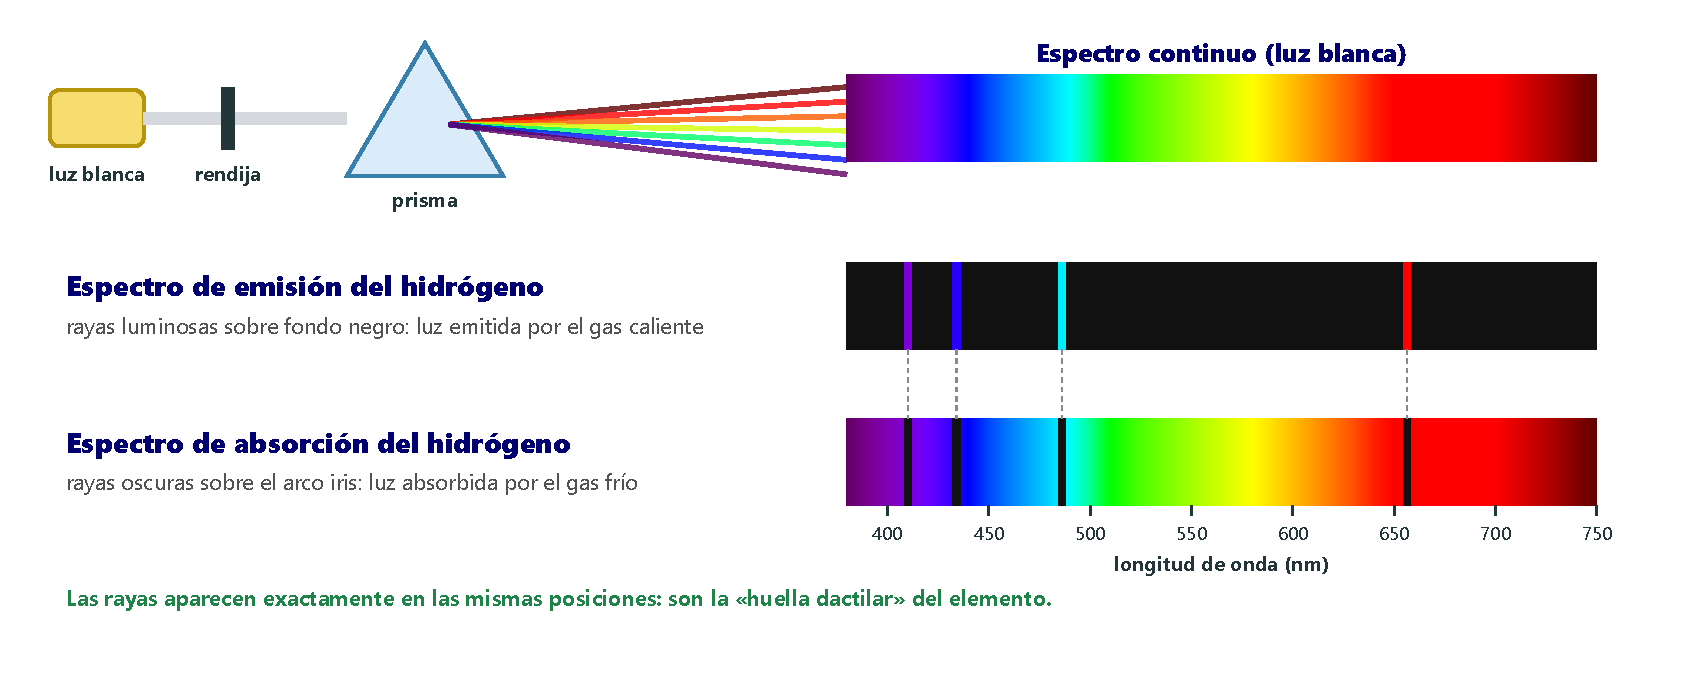
\includegraphics[width=\textwidth]{images/UD2/espectros}
    \caption{Espectro continuo de la luz blanca y espectros de emisión y absorción del hidrógeno.}
    \label{fig:espectros}
\end{figure}

\begin{remark}
    El espectro de cada elemento es \textbf{único}, distinto del de cualquier otro: es su \textbf{«huella dactilar»}. Gracias a ello podemos saber de qué está hecha una estrella sin viajar hasta ella. El helio se descubrió en 1868 en el espectro del Sol, ¡antes que en la Tierra!
\end{remark}

\subsection{¿Por qué el modelo de Rutherford no pudo explicarlos?}

Según el electromagnetismo, una carga eléctrica que se mueve en círculo (y, por tanto, está acelerada) emite energía continuamente en forma de radiación. Si el modelo de Rutherford fuera correcto:
\begin{enumerate}[label=\numberballred]
    \item Los átomos emitirían todo tipo de radiaciones y sus espectros serían \textbf{continuos}, no de rayas.
    \item El electrón, al perder energía, se acercaría cada vez más al núcleo hasta \textbf{caer sobre él}, y el átomo no sería estable. Esto, evidentemente, no ocurre.
\end{enumerate}

\begin{figure}[H]
    \centering
    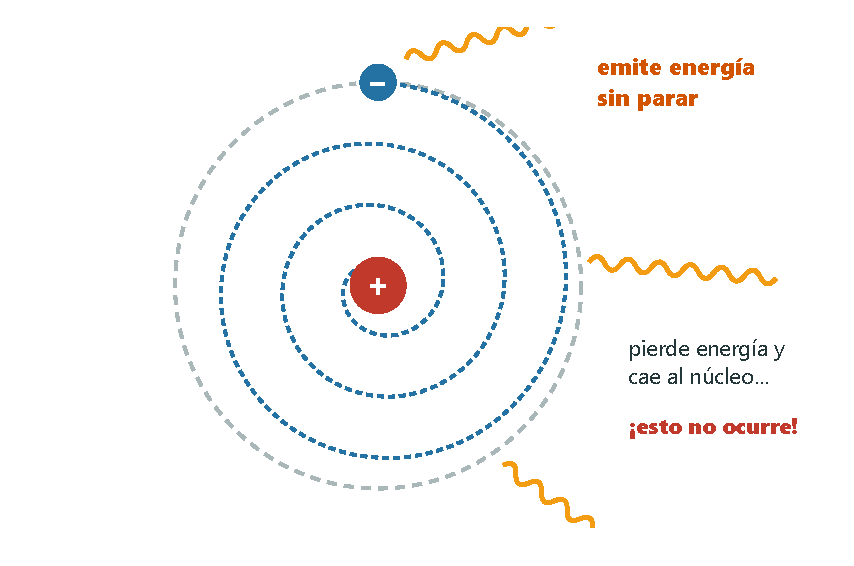
\includegraphics[width=0.5\textwidth]{images/UD2/fallo_rutherford}
    \caption{Según la física clásica, el electrón del modelo de Rutherford debería radiar energía y caer en espiral sobre el núcleo.}
    \label{fig:fallo_rutherford}
\end{figure}

\begin{exercise}
    Clasifica estos espectros en continuos o discontinuos y, en su caso, en espectros de emisión o de absorción:

    \begin{tabular}{rl}
        a) & \espectroabsorcion{0.12,0.2,0.36,0.52,0.6,0.86} \\[4pt]
        b) & \espectrocontinuo \\[4pt]
        c) & \espectroemision{0.18/blue,0.42/green!70!black,0.71/orange,0.83/red}
    \end{tabular}
    \begin{solu}
        \begin{enumerate}[label=\alph*)]
            \item Espectro discontinuo de absorción (rayas oscuras sobre el arco iris).
            \item Espectro continuo.
            \item Espectro discontinuo de emisión (rayas de colores sobre fondo negro).
        \end{enumerate}
    \end{solu}
\end{exercise}

\begin{exercise}
    ¿El espectro de la luz blanca es continuo o de rayas? ¿Y el de la luz emitida por un tubo con gas neón?
    \begin{solu}
        El de la luz blanca es continuo. El del neón, como el de cualquier elemento excitado, es un espectro de emisión de rayas (discontinuo).
    \end{solu}
\end{exercise}

\begin{exercise}
    ¿Es posible que dos elementos químicos distintos tengan exactamente el mismo espectro? Razona tu respuesta.
    \begin{solu}
        No. La distribución de rayas del espectro de cada elemento es única y diferente de la de todos los demás; por eso se usa para identificar elementos.
    \end{solu}
\end{exercise}

\begin{exercise}
    ¿Qué es un espectro atómico de emisión? Explica cómo podríamos obtener el de un elemento concreto.
    \begin{solu}
        Es el conjunto de radiaciones que emiten los átomos de un elemento que ha sido excitado previamente. Se obtiene calentando el elemento o sometiéndolo a una descarga eléctrica (por ejemplo, un gas en un tubo de descarga) y analizando la luz emitida con un espectroscopio.
    \end{solu}
\end{exercise}

\begin{exercise}
    Razona si estos dos espectros pueden pertenecer al mismo elemento:

    \begin{tabular}{rl}
        A & \espectroabsorcion{0.08,0.3,0.5,0.62,0.78,0.9} \\[4pt]
        B & \espectroemision{0.14/violet,0.36/cyan,0.68/orange,0.92/red}
    \end{tabular}
    \begin{solu}
        El A es de absorción y el B de emisión. Si fueran del mismo elemento, las rayas oscuras de A estarían exactamente en las mismas posiciones que las rayas luminosas de B. Como no coinciden, \textcolor{red}{son de elementos distintos}.
    \end{solu}
\end{exercise}

\begin{exercise}
    ¿Pertenecen estos dos espectros al mismo elemento? Indica cuál es de emisión y cuál de absorción.

    \begin{tabular}{rl}
        A & \espectroabsorcion{0.1,0.22,0.47,0.81} \\[4pt]
        B & \espectroemision{0.1/violet,0.22/blue,0.47/cyan,0.81/red}
    \end{tabular}
    \begin{solu}
        \textcolor{red}{Sí}: las rayas oscuras de A están en las mismas posiciones que las rayas luminosas de B. A es el espectro de absorción y B el de emisión.
    \end{solu}
\end{exercise}

%========================================================================================
\section{El modelo de los niveles de energía}
%========================================================================================

En 1913, el físico danés \textbf{Niels Bohr} propuso un nuevo modelo atómico, basado en la existencia de \textbf{niveles de energía} dentro del átomo. Con él explicó la estabilidad del átomo de hidrógeno y su espectro de rayas.

\subsection{Los postulados de Bohr}

\begin{itemize}
    \item \negsubro{Primer postulado.} El electrón solo puede girar en ciertas \textbf{órbitas circulares estables}, en las que se mueve a gran velocidad \textbf{sin emitir energía}. Así se resuelve el problema del modelo de Rutherford: el electrón no cae al núcleo.
    \item \negsubro{Segundo postulado.} En cada órbita, el electrón tiene una \textbf{energía determinada}, que es mayor cuanto más lejos del núcleo está la órbita. Cada órbita es un \textbf{nivel de energía} y se identifica por un número \(n = 1, 2, 3\ldots\)
    \item \negsubro{Tercer postulado.} Mientras está en una órbita estable el electrón no radia energía. Cuando \textbf{baja} de un nivel de mayor energía a otro de menor energía, \textbf{emite} la diferencia en forma de radiación; para \textbf{subir} a un nivel superior, necesita \textbf{absorber} energía.
\end{itemize}

Solo algunas órbitas están permitidas, y los niveles de energía son distintos en cada elemento; por eso sus espectros también lo son.

\subsection{¿Cómo explica el modelo de Bohr los espectros?}

Cuando un átomo recibe energía (por calor o una descarga eléctrica), algunos electrones \textbf{saltan} a niveles más alejados del núcleo. Al volver a niveles inferiores, emiten una energía \textbf{exactamente igual} a la diferencia entre los dos niveles. Por ejemplo, si el electrón pasa del nivel 5 al nivel 1:
\begin{centeredequation*}
    E_{\text{emitida}} = E_5 - E_1
\end{centeredequation*}

Como solo hay unos pocos saltos posibles, solo se emiten unas pocas energías concretas: cada salto produce \textbf{una raya} del espectro.

\begin{figure}[H]
    \centering
    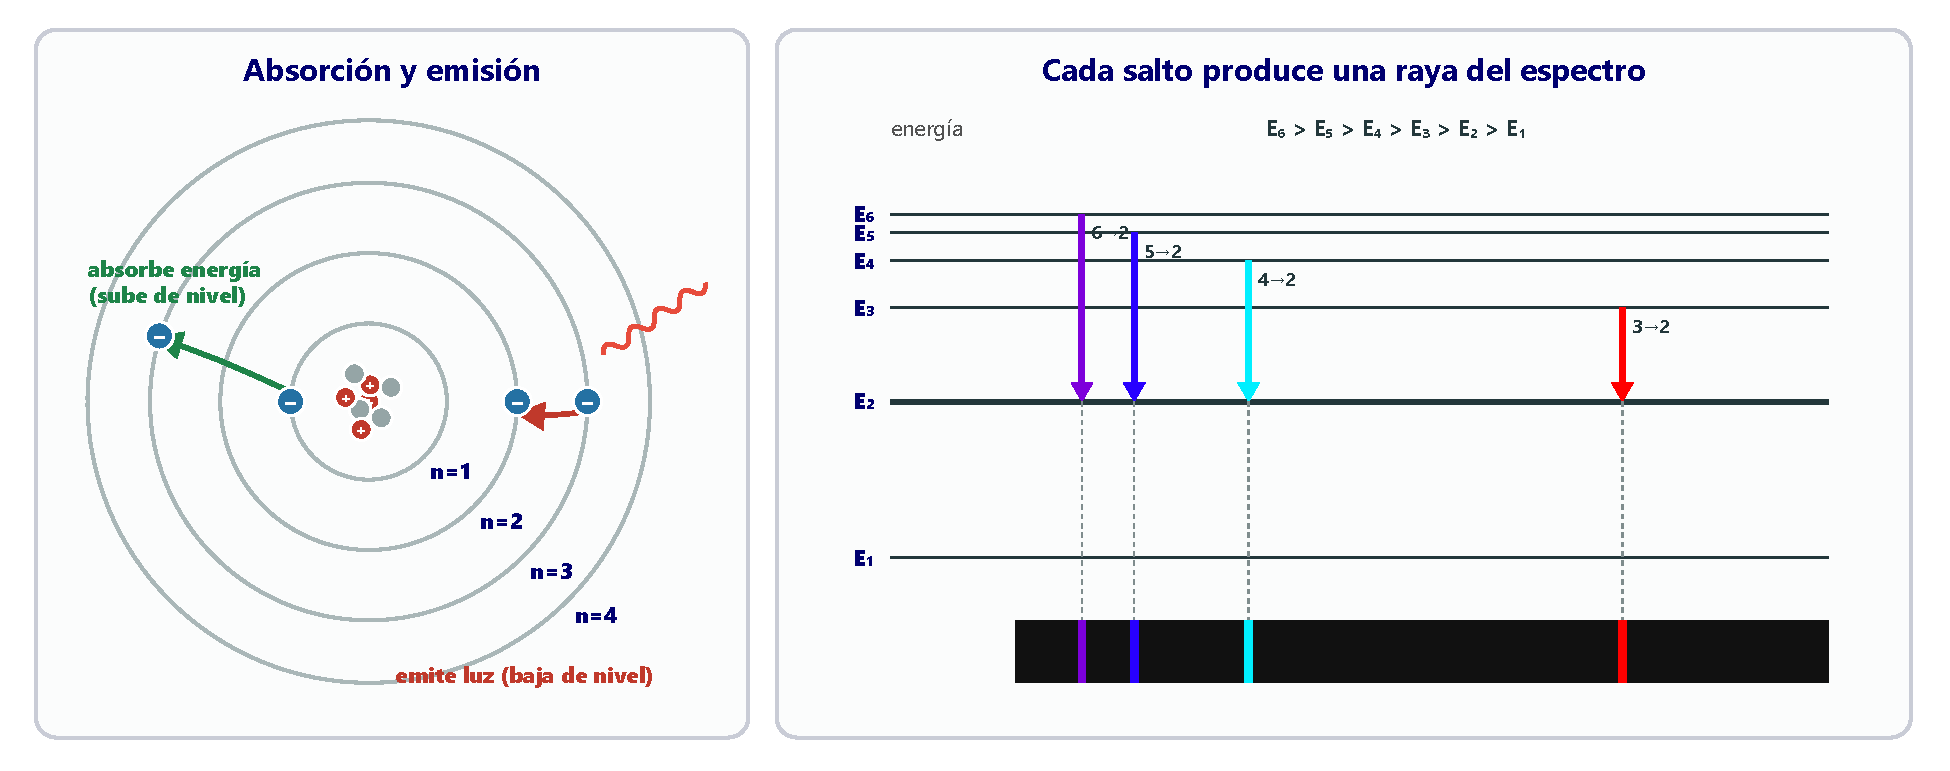
\includegraphics[width=\textwidth]{images/UD2/bohr_saltos}
    \caption{Según Bohr, cada raya del espectro de emisión corresponde a un salto del electrón desde un nivel de energía superior a otro inferior. Las cuatro rayas visibles del hidrógeno se deben a saltos que terminan en el nivel 2.}
    \label{fig:bohr_saltos}
\end{figure}

\subsection{Niveles y subniveles: el modelo de Bohr-Sommerfeld}

Cada nivel puede albergar un número máximo de electrones, que vale \(2n^2\): 2 en el nivel 1, 8 en el nivel 2, 18 en el nivel 3, 32 en el nivel 4\ldots

Con espectroscopios más precisos se vio que muchas rayas eran, en realidad, varias rayas muy juntas. Para explicarlo, \textbf{Arnold Sommerfeld} propuso en 1916 que cada nivel de energía está formado por varios \textbf{subniveles} muy próximos entre sí. Así hay más saltos posibles y aparecen más rayas en el espectro.

Los subniveles se nombran con las letras \textbf{s}, \textbf{p}, \textbf{d} y \textbf{f}, y cada uno admite un número máximo de electrones:

\begin{table}[H]
    \centering
    % --- tabla antigua ---
    % \begin{tblr}{colspec={cccc}, hlines, vlines, row{1}={bg=ocre!85, fg=white, font=\bfseries}, column{1}={bg=ocre!15, font=\bfseries}, cell{1}{1}={bg=ocre!85, fg=white},
        % cell{2}{4}={r=1}{c}, cell{3}{1}={r=2}{c}, cell{3}{4}={r=2}{c}, cell{5}{1}={r=3}{c}, cell{5}{4}={r=3}{c}, cell{8}{1}={r=4}{c}, cell{8}{4}={r=4}{c}}
        % Nivel (\(n\)) & Subniveles & Electrones por subnivel & Electrones por nivel (\(2n^2\)) \\
        % 1 & s & 2 & 2 \\
        % 2 & s & 2 & 8 \\
          % & p & 6 & \\
        % 3 & s & 2 & 18 \\
          % & p & 6 & \\
          % & d & 10 & \\
        % 4 & s & 2 & 32 \\
          % & p & 6 & \\
          % & d & 10 & \\
          % & f & 14 & \\
    % \end{tblr}
    % --- tabla nueva ---
    \begin{tabular}{@{}cccc@{}}
        \toprule
        \textbf{Nivel (\(n\))} & \textbf{Subniveles} & \textbf{Electrones por subnivel} & \textbf{Electrones por nivel (\(2n^2\))} \\
        \midrule
        \textbf{1} & s & 2 & 2 \\[3pt]
        \multirow{2}{*}{\textbf{2}} & s & 2 & \multirow{2}{*}{8} \\[3pt]
         & p & 6 &  \\[3pt]
        \multirow{3}{*}{\textbf{3}} & s & 2 & \multirow{3}{*}{18} \\[3pt]
         & p & 6 &  \\[3pt]
         & d & 10 &  \\[3pt]
        \multirow{4}{*}{\textbf{4}} & s & 2 & \multirow{4}{*}{32} \\[3pt]
         & p & 6 &  \\[3pt]
         & d & 10 &  \\[3pt]
         & f & 14 &  \\
        \bottomrule
    \end{tabular}
    \caption{Capacidad de los niveles y subniveles de energía.}
    \label{tab:subniveles}
\end{table}

\begin{figure}[H]
    \centering
    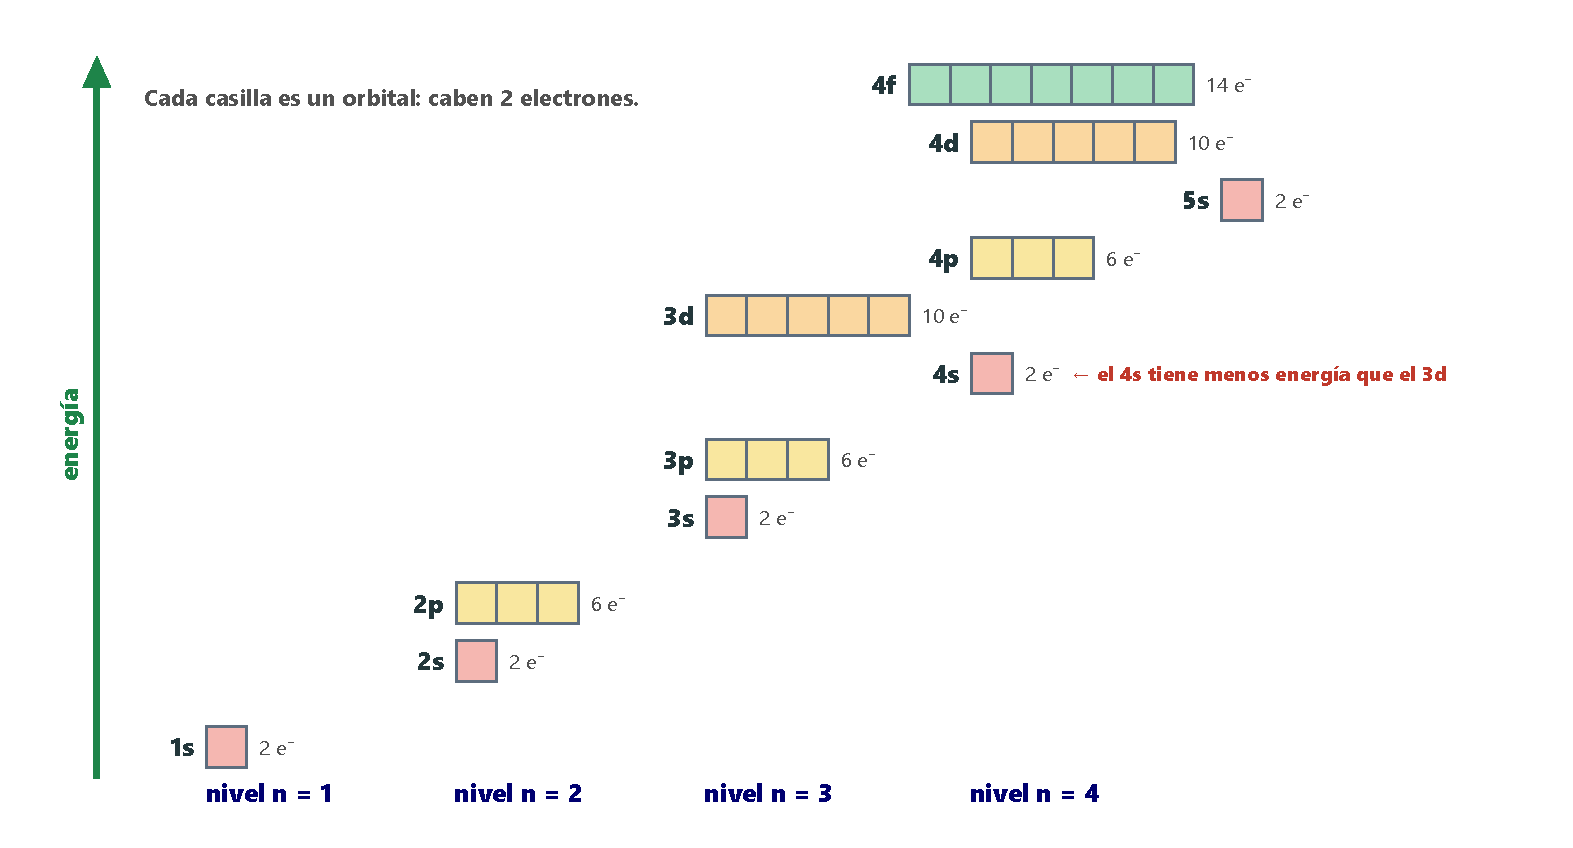
\includegraphics[width=\textwidth]{images/UD2/niveles_subniveles}
    \caption{Desdoblamiento de los niveles en subniveles. Cada casilla representa un orbital, con capacidad para dos electrones. Fíjate en que el subnivel 4s tiene menos energía que el 3d.}
    \label{fig:niveles_subniveles}
\end{figure}

\subsection{La configuración electrónica}

\begin{definition}[Configuración electrónica]
    Es la forma en que se distribuyen los electrones de un átomo en los distintos niveles y subniveles. Los electrones ocupan los subniveles \textbf{de menor a mayor energía}, sin superar la capacidad máxima de cada uno.
\end{definition}

El orden de energía de los subniveles no es simplemente 1, 2, 3\ldots: por ejemplo, el 4s se llena antes que el 3d. Para recordarlo se usa el \textbf{diagrama de Moeller}: se escriben los subniveles en filas y se recorren siguiendo las flechas diagonales.

\begin{figure}[H]
    \centering
    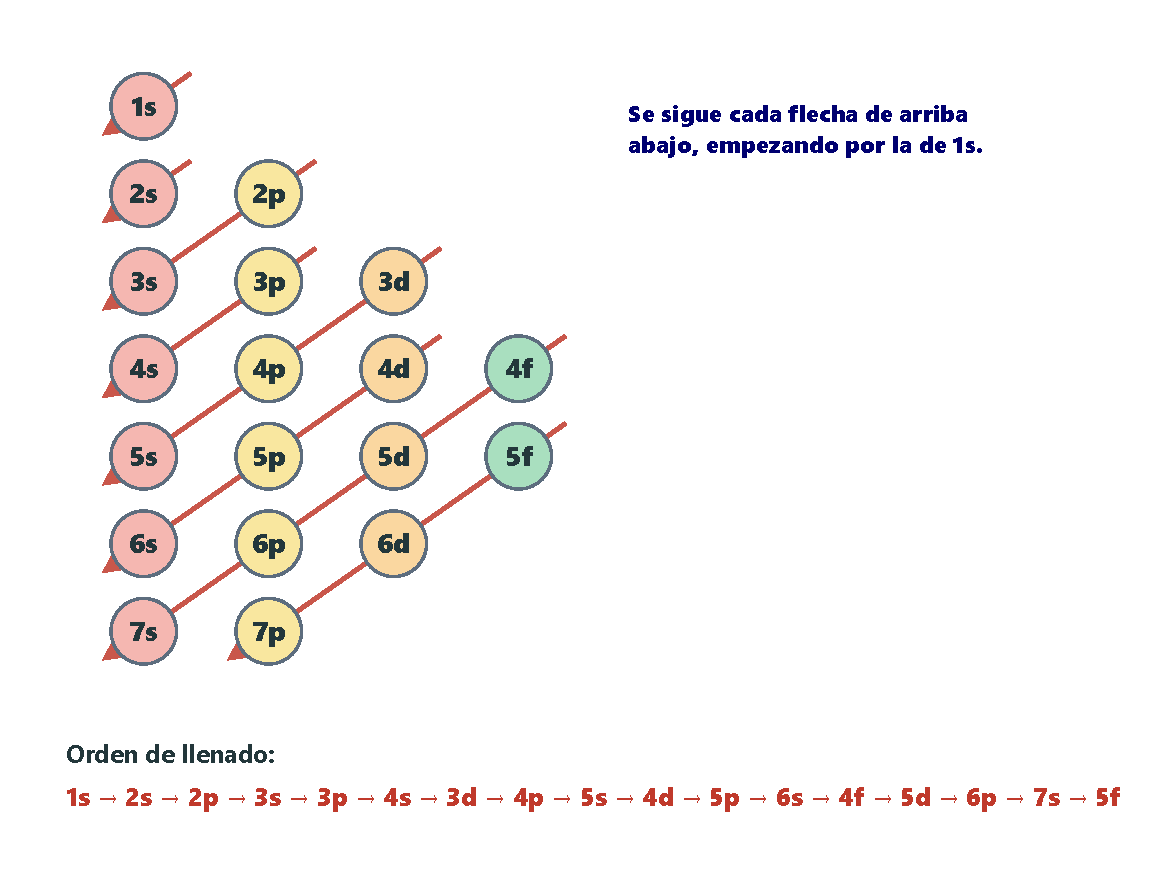
\includegraphics[width=0.7\textwidth]{images/UD2/diagrama_moeller}
    \caption{Diagrama de Moeller: orden de llenado de los subniveles.}
    \label{fig:moeller}
\end{figure}

\begin{example}
    \textbf{Configuración electrónica del sodio.} El sodio tiene \(Z = 11\), es decir, 11 electrones. Llenamos en orden: 2 en el 1s, 2 en el 2s, 6 en el 2p y el que queda en el 3s:
    \begin{centeredequation*}
        \ch{Na}:\ \mathrm{1s^2~2s^2~2p^6~3s^1}
    \end{centeredequation*}
    El exponente indica el número de electrones de cada subnivel; la suma de exponentes debe ser igual al número de electrones (\(2 + 2 + 6 + 1 = 11\)).
\end{example}

\begin{figure}[H]
    \centering
    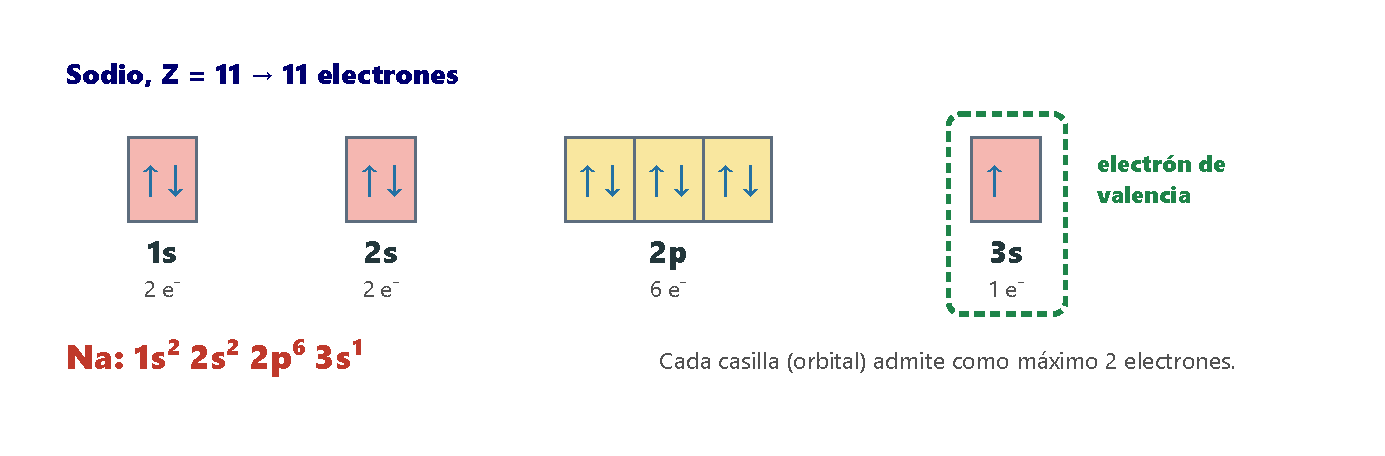
\includegraphics[width=0.75\textwidth]{images/UD2/configuracion_sodio}
    \caption{Diagrama de casillas de la configuración electrónica del sodio.}
    \label{fig:config_sodio}
\end{figure}

\begin{definition}[Electrones de valencia]
    Son los electrones del \textbf{último nivel} de energía ocupado. Por ejemplo, el sodio tiene \textbf{un} electrón de valencia (el del 3s). Son los responsables del comportamiento químico del elemento.
\end{definition}

\begin{remark}
    Para escribir configuraciones largas se puede abreviar usando el \textbf{gas noble} anterior entre corchetes. Por ejemplo, como el neón es \conf{1s^2~2s^2~2p^6}, el sodio queda \conf{[Ne]~3s^1}.
\end{remark}

\begin{exercise}
    ¿Qué cambios introduce el modelo de Bohr respecto al de Rutherford para poder explicar los espectros de rayas, en especial el del hidrógeno?
    \begin{solu}
        Introduce tres postulados: (1) existen órbitas circulares estables en las que el electrón gira sin emitir energía; (2) en cada órbita el electrón tiene una energía determinada, mayor cuanto más alejada está del núcleo; (3) el electrón solo emite (o absorbe) energía al saltar de un nivel a otro, y la energía emitida es la diferencia entre los niveles. Como solo hay ciertos saltos posibles, el espectro es de rayas.
    \end{solu}
\end{exercise}

\begin{exercise}
    Si el electrón no emite energía mientras gira en una órbita estable:
    \begin{enumerate}[label=\alph*)]
        \item ¿Cómo se originan las rayas de los espectros?
        \item ¿Cuándo puede emitir energía un electrón?
    \end{enumerate}
    \begin{solu}
        \begin{enumerate}[label=\alph*)]
            \item Las rayas de emisión se producen cuando un electrón pasa de un nivel superior a otro inferior; las de absorción, cuando pasa de un nivel inferior a otro superior absorbiendo energía.
            \item Solo cuando salta desde un nivel de energía superior a otro inferior.
        \end{enumerate}
    \end{solu}
\end{exercise}

\begin{exercise}
    Representa en tu cuaderno los saltos de energía posibles (hacia niveles inferiores) de un electrón que se encuentra en:
    \begin{enumerate}[label=\alph*)]
        \item El subnivel 3s.
        \item El subnivel 3p.
        \item El subnivel 2p.
    \end{enumerate}
    \begin{solu}
        \begin{enumerate}[label=\alph*)]
            \item Desde el 3s hay \textcolor{red}{tres} saltos posibles: a 2p, a 2s y a 1s.
            \item Desde el 3p hay \textcolor{red}{cuatro} saltos posibles: a 3s, a 2p, a 2s y a 1s.
            \item Desde el 2p hay \textcolor{red}{dos} saltos posibles: a 2s y a 1s.
        \end{enumerate}
    \end{solu}
\end{exercise}

\begin{exercise}
    Escribe la configuración electrónica de estos elementos:
    \begin{multicols}{4}
        \begin{enumerate}[label=\alph*)]
            \item H, \(Z = 1\)
            \item He, \(Z = 2\)
            \item Li, \(Z = 3\)
            \item B, \(Z = 5\)
            \item C, \(Z = 6\)
            \item N, \(Z = 7\)
            \item F, \(Z = 9\)
            \item Ne, \(Z = 10\)
        \end{enumerate}
    \end{multicols}
    \begin{solu}
        \begin{multicols}{2}
            \begin{enumerate}[label=\alph*)]
                \item H: \conf{1s^1}
                \item He: \conf{1s^2}
                \item Li: \conf{1s^2~2s^1}
                \item B: \conf{1s^2~2s^2~2p^1}
                \item C: \conf{1s^2~2s^2~2p^2}
                \item N: \conf{1s^2~2s^2~2p^3}
                \item F: \conf{1s^2~2s^2~2p^5}
                \item Ne: \conf{1s^2~2s^2~2p^6}
            \end{enumerate}
        \end{multicols}
    \end{solu}
\end{exercise}

\begin{exercise}
    Uno de los problemas del modelo de Rutherford era que el electrón, al ser una carga acelerada, debería emitir energía sin parar, lo que es incompatible con los espectros de rayas y con la estabilidad del átomo. ¿Qué postulado de Bohr soluciona este problema y cómo?
    \begin{solu}
        El primero: Bohr afirma que existen órbitas estables en las que el electrón gira a gran velocidad \textbf{sin emitir energía}. Así el electrón no pierde energía ni cae al núcleo.
    \end{solu}
\end{exercise}

\begin{exercise}
    Indica qué afirmaciones son verdaderas y corrige las falsas:
    \begin{enumerate}[label=\alph*)]
        \item El electrón gira muy rápido en una órbita estable en la que no emite energía.
        \item La energía del electrón en una órbita es menor cuanto más lejos del núcleo esté.
        \item Un electrón emite energía solo al pasar de un nivel superior a otro inferior.
        \item Cada elemento tiene un espectro de emisión característico.
        \item El subnivel 3d se llena justo después del 3p.
        \item El subnivel 4p se llena justo después del 4s.
    \end{enumerate}
    \begin{solu}
        \begin{enumerate}[label=\alph*)]
            \item Verdadera.
            \item \textcolor{red}{Falsa.} La energía es \textbf{mayor} cuanto más alejada del núcleo está la órbita.
            \item Verdadera.
            \item Verdadera.
            \item \textcolor{red}{Falsa.} Después del 3p se llena el 4s, y después el 3d.
            \item \textcolor{red}{Falsa.} Después del 4s se llena el 3d, y después el 4p.
        \end{enumerate}
    \end{solu}
\end{exercise}

\begin{exercise}
    Dibuja los dos primeros niveles de energía con sus subniveles. Coloca un electrón en el subnivel de mayor energía y razona cuántas rayas distintas podrían aparecer en el espectro cuando ese electrón vuelva a niveles inferiores.
    \begin{solu}
        Los subniveles son 1s, 2s y 2p (de menor a mayor energía). Un electrón en el 2p puede saltar al 2s o al 1s: aparecerían \textcolor{red}{dos rayas} diferentes. (Si después baja del 2s al 1s se produciría una tercera raya.)
    \end{solu}
\end{exercise}

\begin{exercise}
    ¿En qué subnivel tiene más energía un electrón: en el 2s o en el 3p?
    \begin{solu}
        En el \textcolor{red}{3p}, que pertenece a un nivel superior y se llena después del 2s.
    \end{solu}
\end{exercise}

\begin{exercise}
    Escribe la configuración electrónica de los siguientes átomos y, cuando se indique, de sus iones:
    \begin{multicols}{2}
        \begin{enumerate}[label=\alph*)]
            \item Aluminio (\(Z = 13\)) y \ch{Al^{3+}}
            \item Cloro (\(Z = 17\)) y \ch{Cl-}
            \item Calcio (\(Z = 20\)) y \ch{Ca^{2+}}
            \item Zinc (\(Z = 30\))
            \item Criptón (\(Z = 36\))
            \item Bario (\(Z = 56\)) y \ch{Ba^{2+}}
            \item Polonio (\(Z = 84\))
            \item Lantano (\(Z = 57\))
        \end{enumerate}
    \end{multicols}
    \begin{solu}
        \begin{enumerate}[label=\alph*)]
            \item Al: \conf{1s^2~2s^2~2p^6~3s^2~3p^1}; \quad \ch{Al^{3+}}: \conf{1s^2~2s^2~2p^6}
            \item Cl: \conf{1s^2~2s^2~2p^6~3s^2~3p^5}; \quad \ch{Cl-}: \conf{1s^2~2s^2~2p^6~3s^2~3p^6}
            \item Ca: \conf{1s^2~2s^2~2p^6~3s^2~3p^6~4s^2}; \quad \ch{Ca^{2+}}: \conf{1s^2~2s^2~2p^6~3s^2~3p^6}
            \item Zn: \conf{1s^2~2s^2~2p^6~3s^2~3p^6~4s^2~3d^{10}}
            \item Kr: \conf{1s^2~2s^2~2p^6~3s^2~3p^6~4s^2~3d^{10}~4p^6}
            \item Ba: \conf{[Kr]~5s^2~4d^{10}~5p^6~6s^2}; \quad \ch{Ba^{2+}}: \conf{[Kr]~5s^2~4d^{10}~5p^6}
            \item Po: \conf{[Kr]~5s^2~4d^{10}~5p^6~6s^2~4f^{14}~5d^{10}~6p^4}
            \item La: \conf{[Kr]~5s^2~4d^{10}~5p^6~6s^2~5d^1} (el lantano es una excepción: su último electrón entra en el 5d y no en el 4f).
        \end{enumerate}
    \end{solu}
\end{exercise}

%========================================================================================
\section{¿Cómo se clasifican los elementos químicos? La tabla periódica}
%========================================================================================

Una de las primeras clasificaciones de los elementos los dividía en \textbf{metales} y \textbf{no metales}, según sus propiedades:

\begin{table}[H]
    \centering
    % --- tabla antigua ---
    % \begin{tblr}{colspec={X[l]X[l]}, hlines, vlines, row{1}={bg=ocre!85, fg=white, font=\bfseries, halign=c}}
        % Metales & No metales \\
        % {\textbullet~Tienen brillo metálico.\\ \textbullet~Conducen bien el calor y la electricidad.\\ \textbullet~Son dúctiles (forman hilos) y maleables (forman láminas).\\ \textbullet~Son sólidos a temperatura ambiente, salvo el mercurio.}
        % & {\textbullet~No tienen brillo metálico.\\ \textbullet~Conducen mal el calor y la electricidad.\\ \textbullet~A temperatura ambiente pueden ser sólidos, líquidos o gases.\\ \textbullet~Suelen tener puntos de fusión bajos.} \\
    % \end{tblr}
    % --- tabla nueva ---
    \begin{tabular}{@{}L{0.45\linewidth} L{0.45\linewidth}@{}}
        \toprule
        \textbf{Metales} & \textbf{No metales} \\
        \midrule
        \textbullet~Tienen brillo metálico.\newline \textbullet~Conducen bien el calor y la electricidad.\newline \textbullet~Son dúctiles (forman hilos) y maleables (forman láminas).\newline \textbullet~Son sólidos a temperatura ambiente, salvo el mercurio. & \textbullet~No tienen brillo metálico.\newline \textbullet~Conducen mal el calor y la electricidad.\newline \textbullet~A temperatura ambiente pueden ser sólidos, líquidos o gases.\newline \textbullet~Suelen tener puntos de fusión bajos. \\
        \bottomrule
    \end{tabular}
    \caption{Propiedades generales de metales y no metales.}
    \label{tab:metales}
\end{table}

\subsection{La tabla periódica actual}

Hoy los elementos se organizan en el \textbf{sistema periódico}, ordenados de izquierda a derecha y de arriba abajo por \textbf{número atómico creciente}. La posición de cada elemento depende, por tanto, de su número de protones y, en consecuencia, de su número de electrones.

Los 118 elementos conocidos se reparten en \textbf{18 columnas o grupos} y \textbf{7 filas o períodos}:

\begin{itemize}
    \item \negsubro{Grupos.} Los elementos de una misma columna tienen el \textbf{mismo número de electrones en su último nivel} (electrones de valencia) y, por eso, \textbf{propiedades químicas parecidas}. Se numeran del 1 al 18.
    \item \negsubro{Períodos.} Los elementos de una misma fila tienen el \textbf{mismo número de niveles electrónicos} ocupados, y sus propiedades cambian poco a poco a lo largo de la fila. Se numeran del 1 al 7.
    \begin{itemize}
        \item Períodos \textbf{cortos}: el 1 (2 elementos), el 2 y el 3 (8 elementos cada uno).
        \item Períodos \textbf{largos}: el 4 y el 5 (18 elementos cada uno).
        \item Períodos \textbf{muy largos}: el 6 y el 7 (32 elementos cada uno), que incluyen los lantanoides y actinoides, colocados aparte en dos filas bajo la tabla.
    \end{itemize}
\end{itemize}

\begin{figure}[H]
    \centering
    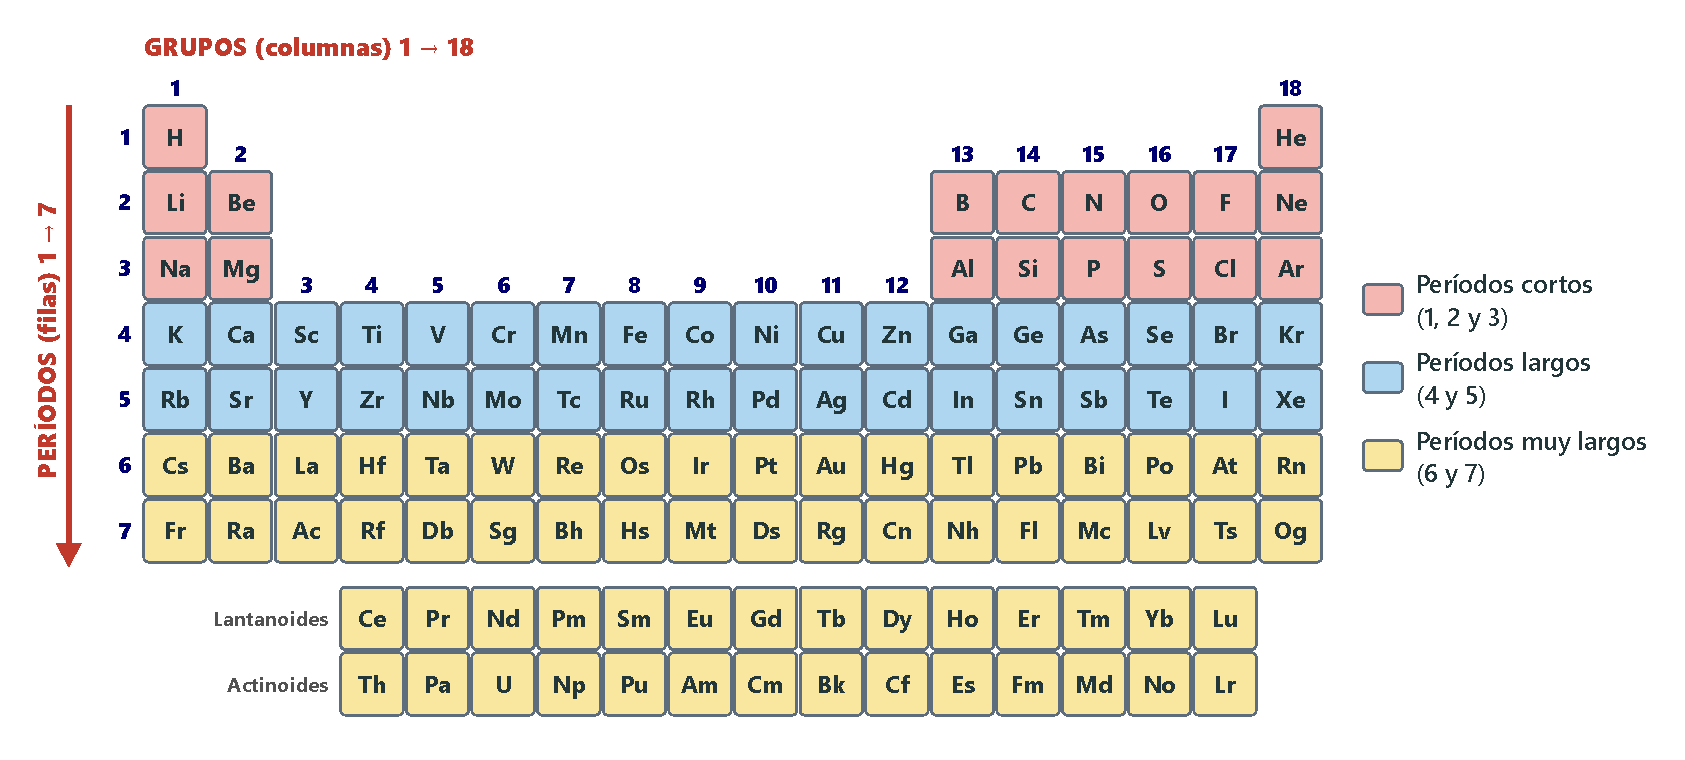
\includegraphics[width=0.9\textwidth]{images/UD2/grupos_periodos}
    \caption{Grupos y períodos de la tabla periódica.}
    \label{fig:grupos_periodos}
\end{figure}

\begin{sidewaysfigure}
    \centering
    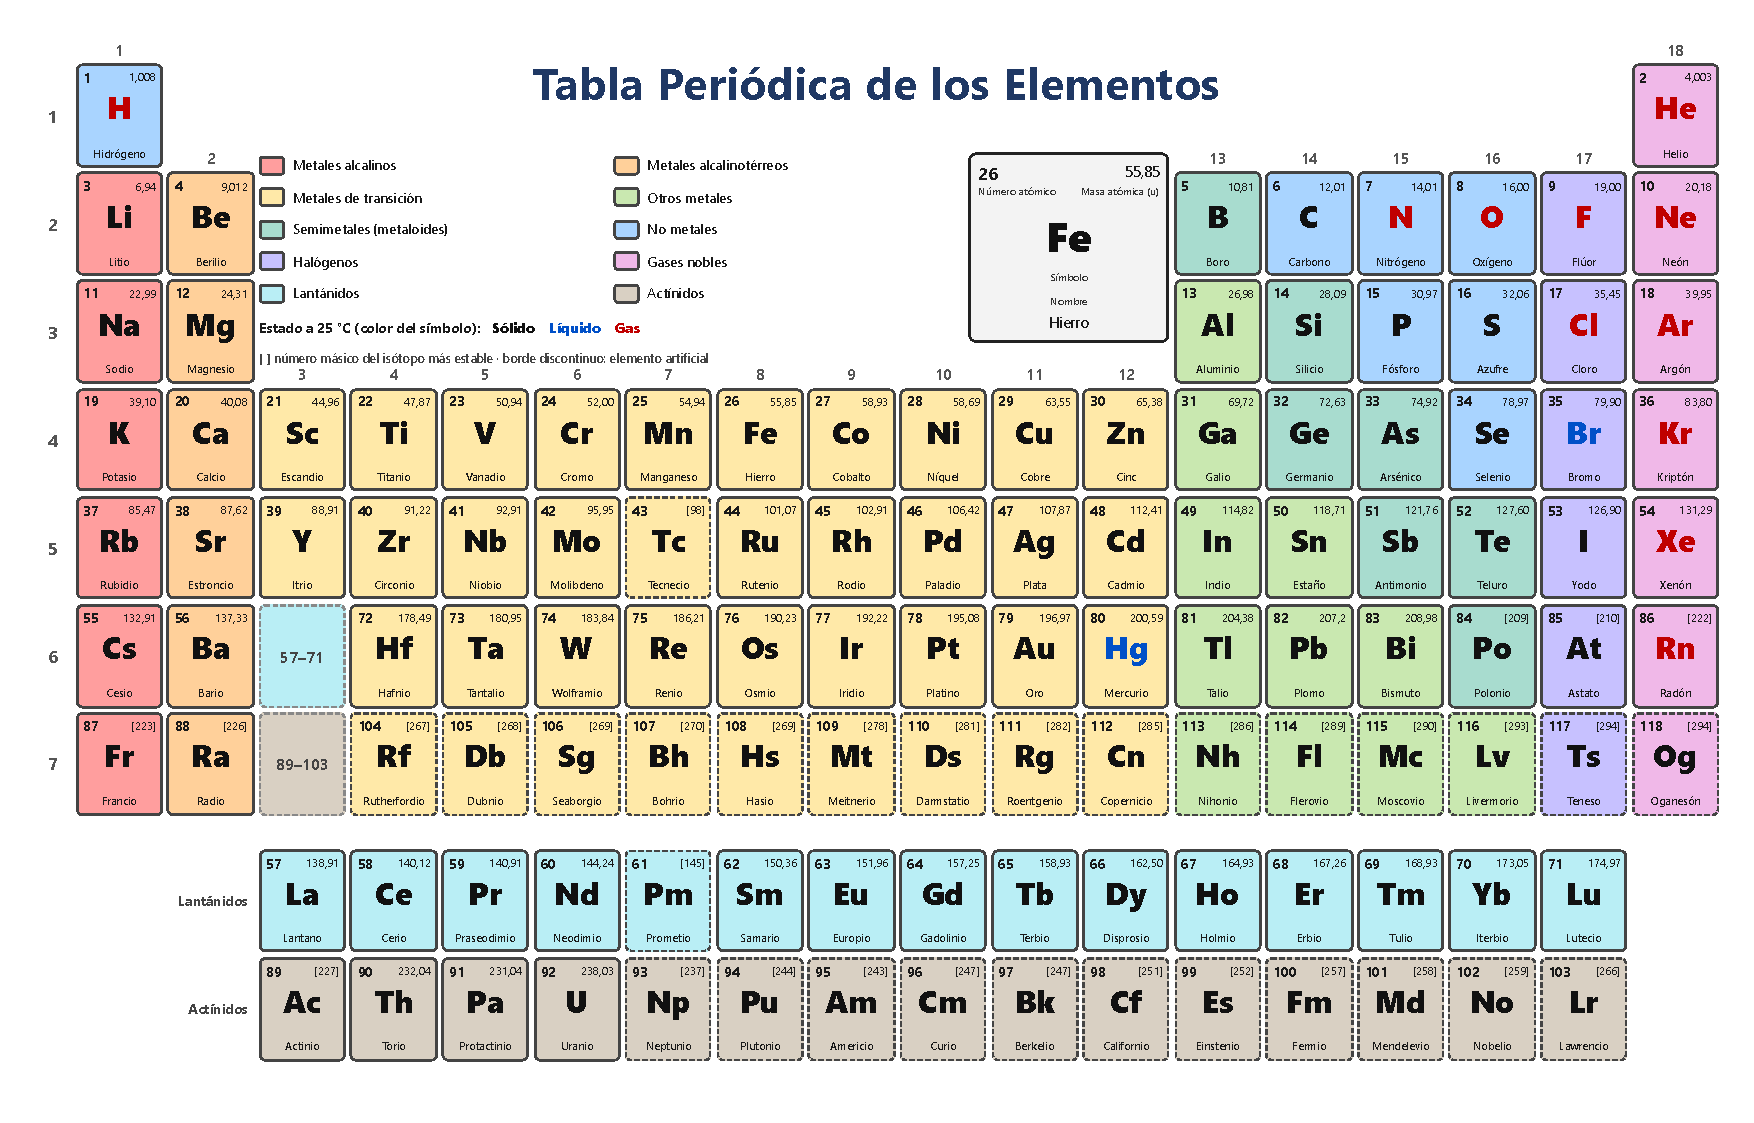
\includegraphics[width=\linewidth,height=0.9\textheight,keepaspectratio]{images/UD2/tabla_periodica}
    \caption{Tabla periódica de los elementos.}
    \label{fig:tabla_periodica}
\end{sidewaysfigure}

\subsection{Regularidades de los elementos en la tabla}

Al ordenar los elementos por número atómico, muchas propiedades se repiten periódicamente.

\paragraph{A lo largo de un período} (de izquierda a derecha):
\begin{itemize}
    \item El número de electrones externos aumenta de uno en uno. El electrón que diferencia a un elemento del anterior se llama \textbf{electrón diferenciador}.
    \item La masa atómica aumenta, salvo alguna excepción.
    \item El carácter metálico disminuye: los metales están a la izquierda y los no metales a la derecha.
    \item Los puntos de fusión y ebullición aumentan hasta la mitad del período y luego disminuyen.
\end{itemize}

\paragraph{Al bajar en un grupo:}
\begin{itemize}
    \item El número de electrones del último nivel es el mismo, por eso las propiedades son similares.
    \item La masa atómica aumenta.
    \item El carácter metálico aumenta.
    \item Los puntos de fusión y ebullición varían ligeramente.
\end{itemize}

\begin{figure}[H]
    \centering
    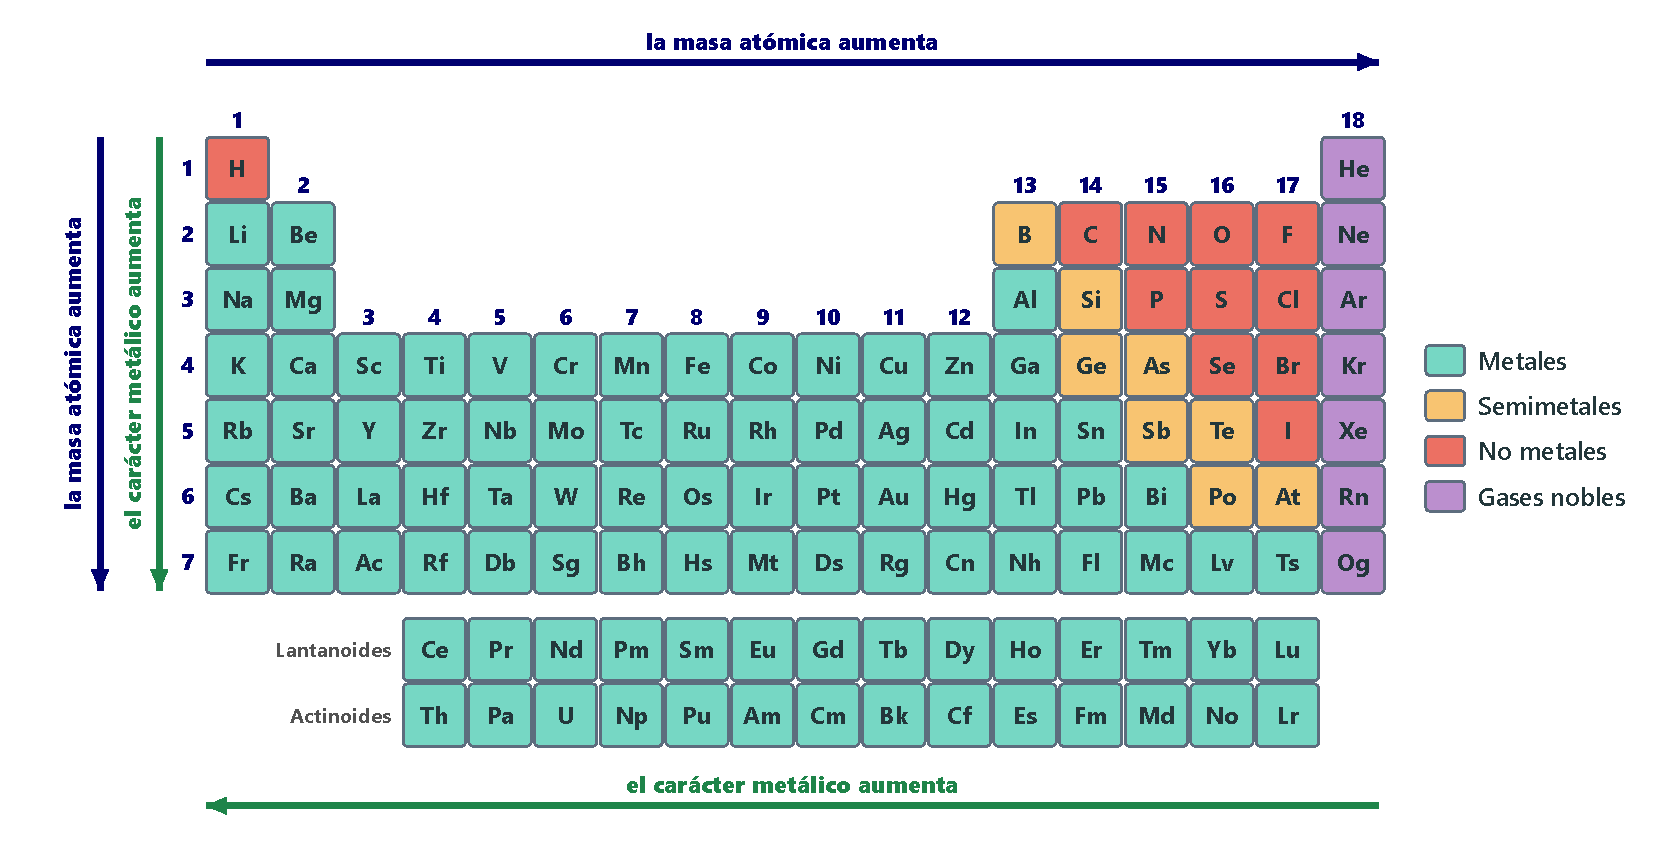
\includegraphics[width=0.95\textwidth]{images/UD2/regularidades}
    \caption{Metales, semimetales, no metales y gases nobles, y variación de la masa atómica y del carácter metálico.}
    \label{fig:regularidades}
\end{figure}

\begin{table}[H]
    \centering
    % --- tabla antigua ---
    % \begin{tblr}{colspec={lll}, row{1}={bg=ocre!85, fg=white, font=\bfseries}, hlines}
        % Grupos 1 a 6 & Grupos 7 a 12 & Grupos 13 a 18 \\
        % 1. Alcalinos & 7. Familia del manganeso & 13. Térreos (familia del boro) \\
        % 2. Alcalinotérreos & 8. Familia del hierro & 14. Carbonoideos \\
        % 3. Familia del escandio & 9. Familia del cobalto & 15. Nitrogenoideos \\
        % 4. Familia del titanio & 10. Familia del níquel & 16. Anfígenos \\
        % 5. Familia del vanadio & 11. Familia del cobre & 17. Halógenos \\
        % 6. Familia del cromo & 12. Familia del zinc & 18. Gases nobles \\
    % \end{tblr}
    % --- tabla nueva ---
    \begin{tabular}{@{}lll@{}}
        \toprule
        \textbf{Grupos 1 a 6} & \textbf{Grupos 7 a 12} & \textbf{Grupos 13 a 18} \\
        \midrule
        1. Alcalinos & 7. Familia del manganeso & 13. Térreos (familia del boro) \\[3pt]
        2. Alcalinotérreos & 8. Familia del hierro & 14. Carbonoideos \\[3pt]
        3. Familia del escandio & 9. Familia del cobalto & 15. Nitrogenoideos \\[3pt]
        4. Familia del titanio & 10. Familia del níquel & 16. Anfígenos \\[3pt]
        5. Familia del vanadio & 11. Familia del cobre & 17. Halógenos \\[3pt]
        6. Familia del cromo & 12. Familia del zinc & 18. Gases nobles \\
        \bottomrule
    \end{tabular}
    \caption{Nombres de los grupos de la tabla periódica.}
    \label{tab:nombres_grupos}
\end{table}

\subsection{Configuración electrónica y posición en la tabla}

La tabla periódica es, en realidad, un mapa de las configuraciones electrónicas. Veamos cómo se van llenando los subniveles período a período:

\begin{itemize}
    \item \negsubro{Período 1.} El hidrógeno (\conf{1s^1}) y el helio (\conf{1s^2}) llenan el subnivel 1s, que solo admite dos electrones.
    \item \negsubro{Período 2.} Del litio (\conf{1s^2~2s^1}) al neón se llenan el 2s y el 2p: \(2 + 6 = 8\) electrones, 8 elementos.
    \item \negsubro{Período 3.} Se repite el proceso con el 3s y el 3p, del sodio (\conf{[Ne]~3s^1}) al argón (\conf{[Ne]~3s^2~3p^6}).
    \item \negsubro{Período 4.} El potasio y el calcio colocan sus electrones en el 4s (que tiene menos energía que el 3d). Desde el escandio hasta el zinc se llena el 3d (10 elementos) y, después, el 4p, hasta el criptón: 18 elementos.
    \item \negsubro{Período 5.} Se llenan el 5s (Rb y Sr), el 4d (del Y al Cd) y el 5p (del In al Xe): 18 elementos.
    \item \negsubro{Período 6.} El cesio y el bario llenan el 6s. El lantano coloca un electrón en el 5d, pero a partir del cerio se llena el \textbf{4f} (14 elementos, los \textbf{lantanoides}). Después se completa el 5d (del Hf al Hg) y el 6p (del Tl al Rn).
    \item \negsubro{Período 7.} Ocurre algo análogo: 7s, un electrón en el 6d (actinio), el \textbf{5f} desde el torio (los \textbf{actinoides}), y después el 6d y el 7p.
\end{itemize}

\begin{figure}[H]
    \centering
    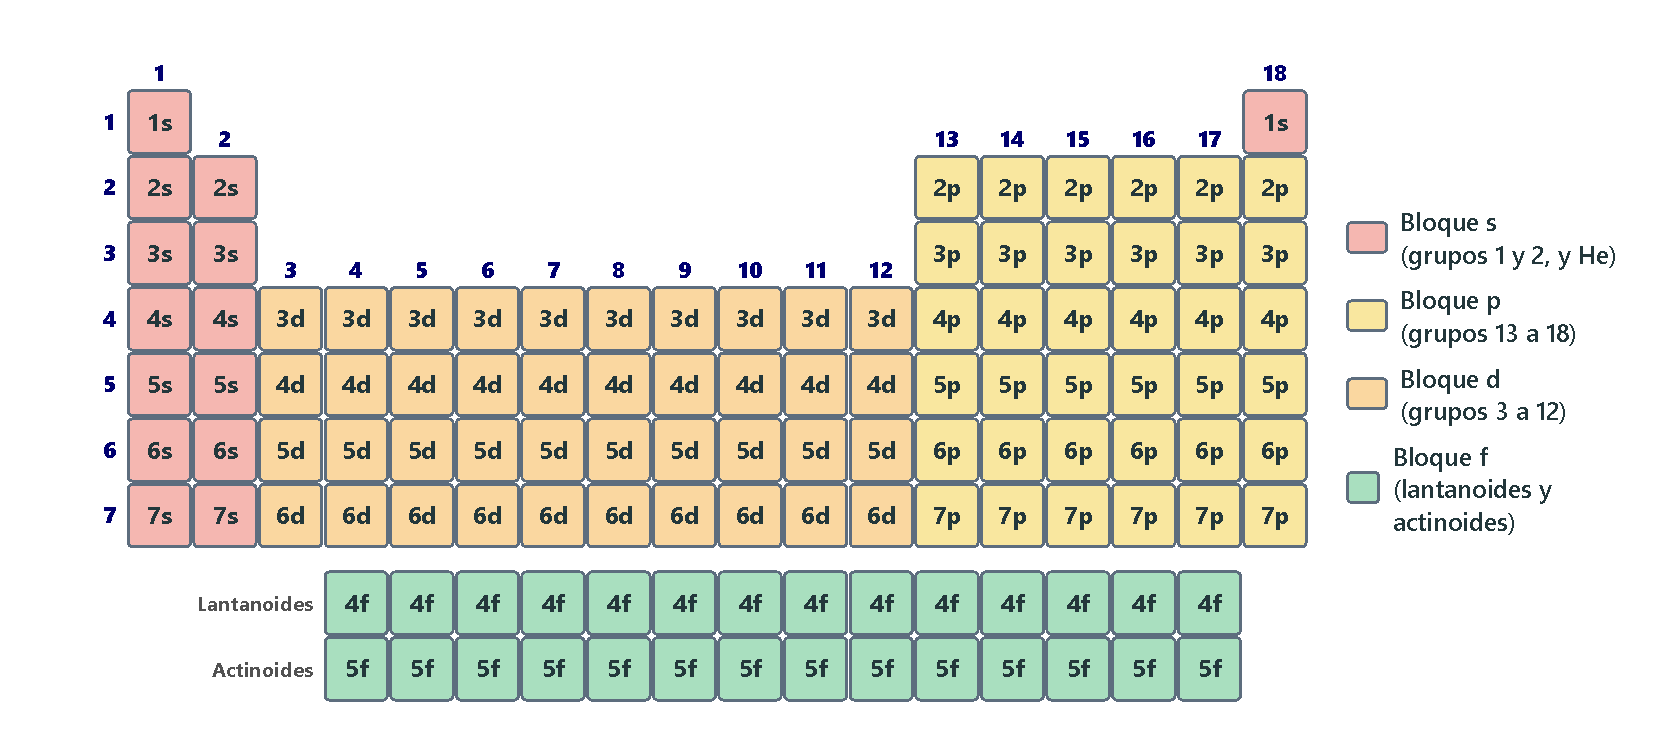
\includegraphics[width=0.9\textwidth]{images/UD2/bloques_spdf}
    \caption{Subnivel que ocupa el electrón diferenciador en cada zona de la tabla: bloques s, p, d y f.}
    \label{fig:bloques}
\end{figure}

\begin{remark}
    \textbf{Truco para leer la tabla:} el número del \textbf{período} coincide con el último nivel ocupado (el número más alto de la configuración), y en los elementos de los bloques s y p los \textbf{electrones de valencia} se deducen del grupo: 1 en el grupo 1, 2 en el grupo 2, y \(\text{grupo} - 10\) en los grupos 13 a 18 (salvo el helio, que tiene 2).
\end{remark}

\begin{exercise}
    Escribe el nombre de cinco elementos metálicos y de cinco no metálicos.
    \begin{solu}
        Respuesta libre. Por ejemplo, metales: hierro, cobre, sodio, aluminio, oro. No metales: oxígeno, nitrógeno, carbono, azufre, cloro.
    \end{solu}
\end{exercise}

\begin{exercise}
    Nombra tres elementos situados en:
    \begin{multicols}{2}
        \begin{enumerate}[label=\alph*)]
            \item Un período corto.
            \item Un período largo.
            \item Un período muy largo.
            \item El grupo 18.
            \item El período 5.
        \end{enumerate}
    \end{multicols}
    \begin{solu}
        Respuesta libre. Por ejemplo: a) sodio, aluminio, fósforo; b) hierro, cadmio, indio; c) cesio, osmio, oro; d) helio, neón, argón; e) itrio, plata, yodo.
    \end{solu}
\end{exercise}

\begin{exercise}
    Indica el grupo y el período de cada uno de estos elementos: fósforo, bromo, estroncio, rutenio, xenón, cesio, mercurio, lantano y actinio.
    \begin{solu}
        Fósforo: grupo 15, período 3. Bromo: grupo 17, período 4. Estroncio: grupo 2, período 5. Rutenio: grupo 8, período 5. Xenón: grupo 18, período 5. Cesio: grupo 1, período 6. Mercurio: grupo 12, período 6. Lantano: grupo 3, período 6. Actinio: grupo 3, período 7.
    \end{solu}
\end{exercise}

\begin{exercise}
    ¿Cuáles de estos elementos tienen el mismo número de electrones de valencia? Litio, calcio, cloro, rubidio, neón, sodio, hierro, cesio, plomo, potasio.
    \begin{solu}
        Litio, rubidio, sodio, cesio y potasio: todos son del grupo 1 y tienen \textcolor{red}{un electrón de valencia}.
    \end{solu}
\end{exercise}

\begin{exercise}
    En cada pareja, ¿cuál tiene mayor carácter metálico?
    \begin{multicols}{4}
        \begin{enumerate}[label=\alph*)]
            \item Be / Ba
            \item F / I
            \item Sc / Zn
            \item C / Pb
            \item Cu / Au
            \item Li / Cs
            \item Pd / I
            \item B / In
        \end{enumerate}
    \end{multicols}
    \begin{solu}
        \textcolor{blue}{El carácter metálico aumenta hacia abajo en un grupo y hacia la izquierda en un período.}
        a) Ba; b) I; c) Sc; d) Pb; e) Au; f) Cs; g) Pd; h) In.
    \end{solu}
\end{exercise}

\begin{exercise}
    Nombra cinco elementos con el mismo número de niveles electrónicos que el azufre (\(Z = 16\)).
    \begin{solu}
        El azufre está en el período 3, así que tiene 3 niveles. Por ejemplo: sodio, magnesio, aluminio, silicio y fósforo (también cloro y argón).
    \end{solu}
\end{exercise}

\begin{exercise}
    Indica a qué familia pertenece cada elemento: cloro, cesio, silicio, fósforo, magnesio, argón.
    \begin{solu}
        Cloro: halógenos. Cesio: alcalinos. Silicio: carbonoideos. Fósforo: nitrogenoideos. Magnesio: alcalinotérreos. Argón: gases nobles.
    \end{solu}
\end{exercise}

\begin{exercise}
    Nombra cinco elementos con el mismo número de electrones en el último nivel que el aluminio (\(Z = 13\)).
    \begin{solu}
        Los del grupo 13: boro, galio, indio, talio y nihonio.
    \end{solu}
\end{exercise}

\begin{exercise}
    ¿Cuántos niveles electrónicos tienen los átomos que van del litio al neón? ¿Y los que van del sodio al argón?
    \begin{solu}
        Del litio al neón (período 2): \textcolor{red}{dos niveles}. Del sodio al argón (período 3): \textcolor{red}{tres niveles}.
    \end{solu}
\end{exercise}

\begin{exercise}
    ¿Cómo cambia el número de electrones del último nivel al pasar de un elemento al siguiente dentro de un período?
    \begin{solu}
        Aumenta de uno en uno (el electrón diferenciador).
    \end{solu}
\end{exercise}

\begin{exercise}
    El electrón diferenciador es el que distingue a un elemento del anterior. Indica en qué subnivel se encuentra el electrón diferenciador de: litio, neón, magnesio, escandio, bromo, rubidio, circonio, yodo, lantano, cerio, actinio y torio.
    \begin{solu}
        Litio: 2s. Neón: 2p. Magnesio: 3s. Escandio: 3d. Bromo: 4p. Rubidio: 5s. Circonio: 4d. Yodo: 5p. Lantano: 5d. Cerio: 4f. Actinio: 6d. Torio: 5f.
    \end{solu}
\end{exercise}

\begin{exercise}
    ¿Qué elemento es más metálico, el sodio o el cesio? ¿Y cuál es más no metálico, el carbono o el flúor?
    \begin{solu}
        El \textcolor{red}{cesio} es más metálico (está más abajo en el grupo 1). El \textcolor{red}{flúor} es más no metálico (está más a la derecha en el período 2).
    \end{solu}
\end{exercise}

\begin{exercise}
    Escribe el nombre, el símbolo y el número atómico de tres elementos que:
    \begin{enumerate}[label=\alph*)]
        \item Tengan el mismo número de niveles que el silicio.
        \item Tengan sus electrones repartidos en cuatro niveles.
        \item Pertenezcan a un período corto.
    \end{enumerate}
    \begin{solu}
        Respuesta libre. Por ejemplo: a) sodio, Na, 11; azufre, S, 16; cloro, Cl, 17. b) Cualquiera del período 4: potasio, K, 19; hierro, Fe, 26; bromo, Br, 35. c) Cualquiera de los períodos 1, 2 o 3: helio, He, 2; carbono, C, 6; magnesio, Mg, 12.
    \end{solu}
\end{exercise}

\begin{exercise}
    Escribe la configuración electrónica de los gases nobles. ¿Qué tienen todos en común?
    \begin{solu}
        He: \conf{1s^2}\\
        Ne: \conf{1s^2~2s^2~2p^6}\\
        Ar: \conf{1s^2~2s^2~2p^6~3s^2~3p^6}\\
        Kr: \conf{[Ar]~4s^2~3d^{10}~4p^6}\\
        Xe: \conf{[Kr]~5s^2~4d^{10}~5p^6}\\
        Rn: \conf{[Xe]~6s^2~4f^{14}~5d^{10}~6p^6}\\
        Todos tienen su último nivel completo: 8 electrones (\conf{ns^2~np^6}), salvo el helio, que tiene 2.
    \end{solu}
\end{exercise}

\begin{exercise}
    Explica por qué la configuración electrónica del ion \ch{Na+} es \conf{1s^2~2s^2~2p^6}.
    \begin{solu}
        El sodio neutro es \conf{1s^2~2s^2~2p^6~3s^1}. Al perder su electrón de valencia (el del 3s) se forma \ch{Na+}, que queda con \conf{1s^2~2s^2~2p^6}, la misma configuración que el neón.
    \end{solu}
\end{exercise}

\begin{exercise}
    Explica por qué la configuración del ion \ch{Cl-} es \conf{1s^2~2s^2~2p^6~3s^2~3p^6}.
    \begin{solu}
        El cloro neutro es \conf{1s^2~2s^2~2p^6~3s^2~3p^5}. Al ganar un electrón, este entra en el 3p, que queda completo con 6 electrones: es la configuración del argón.
    \end{solu}
\end{exercise}

\begin{exercise}
    ¿A qué elemento corresponde la configuración \conf{1s^2~2s^2~2p^6~3s^2~3p^3}?
    \begin{solu}
        \textcolor{blue}{Sumamos los electrones: \(2 + 2 + 6 + 2 + 3 = 15\).} Es el \textcolor{red}{fósforo, \(Z = 15\)}.
    \end{solu}
\end{exercise}

\begin{exercise}
    Dibuja el contorno de la tabla periódica en tu cuaderno y señala el grupo de los alcalinotérreos. Después escribe:
    \begin{enumerate}[label=\alph*)]
        \item La configuración de su último nivel.
        \item La configuración de sus iones cuando pierden dos electrones.
    \end{enumerate}
    \begin{solu}
        \begin{enumerate}[label=\alph*)]
            \item \conf{ns^2}, donde \(n\) es el número del período.
            \item Al perder los dos electrones del \conf{ns^2}, cada ion queda con la configuración del gas noble anterior (por ejemplo, \ch{Mg^{2+}}: \conf{1s^2~2s^2~2p^6}, como el neón).
        \end{enumerate}
    \end{solu}
\end{exercise}

\begin{exercise}
    Localiza el grupo 16 (anfígenos) y escribe la configuración electrónica de su último nivel.
    \begin{solu}
        \conf{ns^2~np^4}: tienen 6 electrones de valencia.
    \end{solu}
\end{exercise}

\begin{exercise}
    Sobre los elementos del grupo 18:
    \begin{enumerate}[label=\alph*)]
        \item ¿Cuántos electrones tienen en su último nivel?
        \item ¿Cuántos electrones caben como máximo en los subniveles s y p de ese último nivel?
    \end{enumerate}
    \begin{solu}
        a) 8 electrones (el helio, 2). b) 8 (2 en el s y 6 en el p): el último nivel está completo, por eso son muy estables.
    \end{solu}
\end{exercise}

\begin{exercise}
    Sobre los elementos del grupo 1:
    \begin{enumerate}[label=\alph*)]
        \item ¿Cuántos electrones tienen en su último nivel?
        \item ¿Cuántos tendrían que perder para quedarse con el último nivel completo?
        \item ¿Son metales o no metales?
        \item ¿Cómo se llama este grupo?
    \end{enumerate}
    \begin{solu}
        a) Un electrón (\conf{ns^1}). b) Uno: al perderlo quedan con la configuración del gas noble anterior. c) Son metales (excepto el hidrógeno). d) Alcalinos.
    \end{solu}
\end{exercise}

\begin{exercise}
    Sobre los elementos del grupo 15:
    \begin{enumerate}[label=\alph*)]
        \item ¿Cuántos electrones tienen en su último nivel?
        \item ¿Les conviene ganar o perder electrones para completar ese nivel? ¿Cuántos?
        \item ¿Son metales o no metales?
    \end{enumerate}
    \begin{solu}
        a) Cinco (\conf{ns^2~np^3}). b) Ganar tres electrones. c) El nitrógeno y el fósforo son no metales; el arsénico y el antimonio, semimetales; el bismuto, un metal.
    \end{solu}
\end{exercise}

\begin{exercise}
    Los elementos que forman parte de los seres vivos se llaman bioelementos. Investiga cuáles son, en qué proporción están en el cuerpo humano y qué funciones cumplen.
    \begin{solu}
        Respuesta libre. Los principales son C, H, O y N (más del \qty{95}{\percent} de la masa), junto con P y S. Otros, en menor cantidad: Ca (huesos), Na y K (impulso nervioso), Fe (hemoglobina), Mg, Cl, I (tiroides)\ldots
    \end{solu}
\end{exercise}

\begin{exercise}
    ¿Qué elemento es el primero en empezar a llenar cada uno de estos subniveles?
    \begin{multicols}{5}
        \begin{enumerate}[label=\alph*)]
            \item 3p
            \item 4s
            \item 4d
            \item 5d
            \item 4f
        \end{enumerate}
    \end{multicols}
    \begin{solu}
        a) Aluminio. b) Potasio. c) Itrio. d) Lantano. e) Cerio.
    \end{solu}
\end{exercise}

%========================================================================================
\section{Tipos de elementos químicos}
%========================================================================================

Según el subnivel en el que se aloja su electrón diferenciador, los elementos se clasifican en tres tipos: \textbf{representativos}, \textbf{de transición} y \textbf{de transición interna}.

\begin{figure}[H]
    \centering
    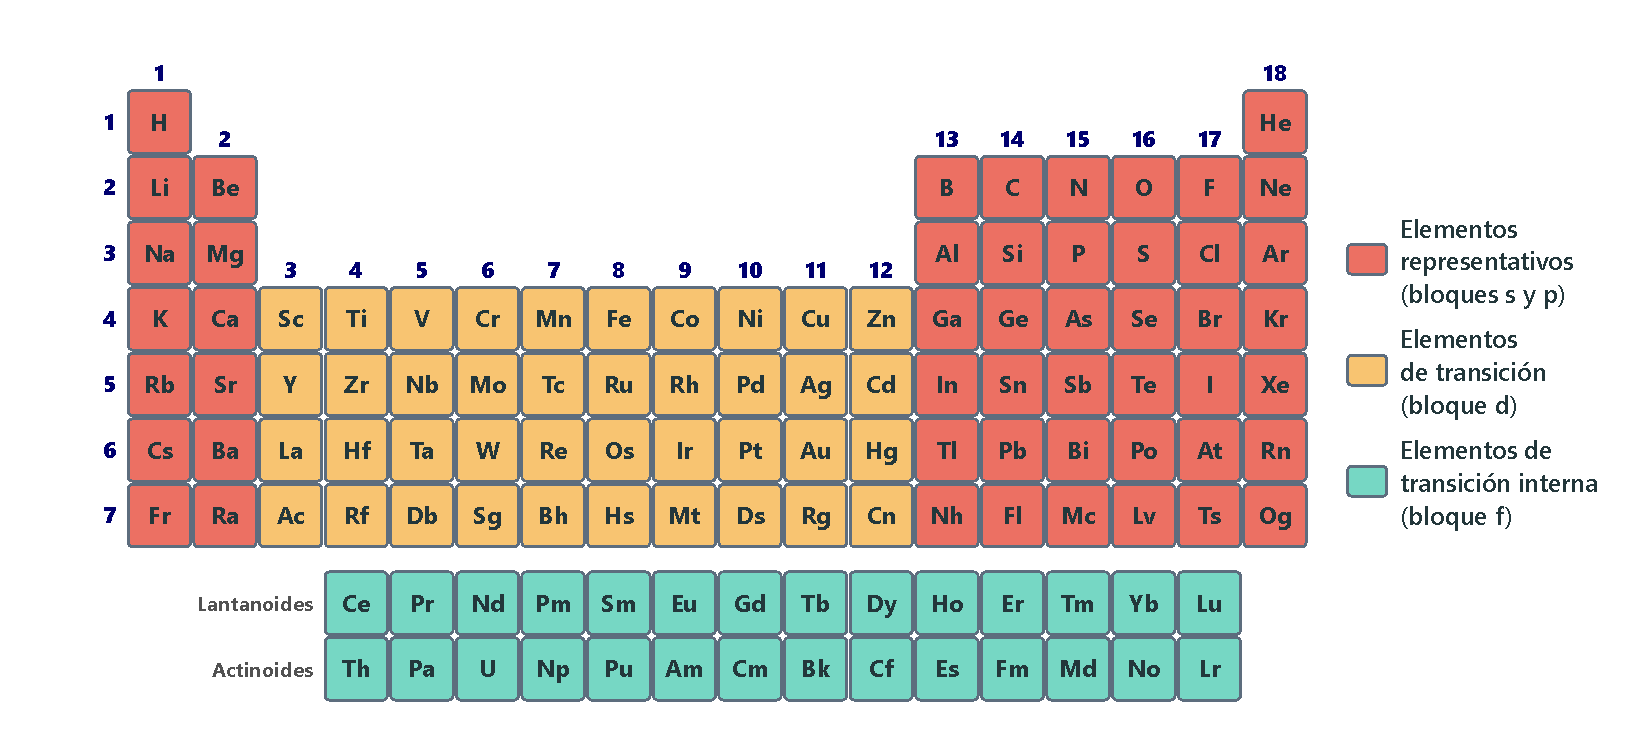
\includegraphics[width=0.9\textwidth]{images/UD2/tipos_elementos}
    \caption{Tipos de elementos según su configuración electrónica.}
    \label{fig:tipos_elementos}
\end{figure}

\subsection{Los elementos representativos}

Su configuración electrónica externa va desde \conf{ns^1} hasta \conf{ns^2~np^6}: solo ocupan los subniveles s y p del último nivel. Son los más abundantes en la Tierra y en el universo. Se distinguen tres bloques:

\begin{itemize}
    \item El \textbf{bloque s}: grupos 1 y 2.
    \item El \textbf{bloque p}: grupos 13 a 17.
    \item Los \textbf{gases nobles} (grupo 18), con configuración \conf{ns^2~np^6}, de máxima estabilidad.
\end{itemize}

\subsection{Metales, no metales y semimetales}

El hidrógeno y el helio, del primer período, son no metales. En el resto de períodos, los elementos representativos pasan de \textbf{metales} (a la izquierda) a \textbf{no metales} (a la derecha), pasando por los \textbf{semimetales}.

\begin{itemize}
    \item Los átomos \textbf{metálicos} tienen pocos electrones externos y los pierden con facilidad.
    \item Los \textbf{no metálicos} tienen más electrones en su última capa, más fuertemente retenidos; tienden a ganarlos.
    \item Los \textbf{semimetales} (B, Si, Ge, As, Sb, Te\ldots) tienen propiedades intermedias: por ejemplo, son \textbf{semiconductores}, por eso se usan en los chips electrónicos.
\end{itemize}

\subsection{Los elementos de transición}

Son aquellos cuyo último electrón entra en un subnivel \textbf{d}: forman el \textbf{bloque d}. Su configuración externa va de \conf{(n-1)d^1~ns^2} a \conf{(n-1)d^{10}~ns^2}. Ocupan la parte central de la tabla, los grupos 3 a 12 (diez grupos, uno por cada electrón d). Sus propiedades comunes son:

\begin{itemize}
    \item Todos son \textbf{metales}.
    \item Son sólidos, excepto el mercurio, que es líquido.
    \item Son duros y tienen puntos de fusión y ebullición elevados.
    \item Son muy buenos conductores del calor y de la electricidad.
    \item Sus compuestos suelen tener \textbf{colores} llamativos.
\end{itemize}

\subsection{Los elementos de transición interna}

Al llenarse los subniveles \textbf{4f} y \textbf{5f} aparecen dos series de catorce elementos, el \textbf{bloque f}, que se sitúan en las dos filas separadas de la parte inferior de la tabla. Sus propiedades se parecen a las de los metales de transición.

\begin{itemize}
    \item \negsubro{Lantanoides.} Del cerio (\(Z = 58\)) al lutecio (\(Z = 71\)). Llenan el 4f: por ejemplo, el cerio es \conf{[Xe]~6s^2~5d^1~4f^1}. Todos existen en la naturaleza salvo el prometio. El lantano (\(Z = 57\)) es del bloque d (\conf{[Xe]~6s^2~5d^1}).
    \item \negsubro{Actinoides.} Del torio (\(Z = 90\)) al laurencio (\(Z = 103\)). Llenan el 5f. Todos son radiactivos y, a partir del uranio (\(Z = 92\)), se obtienen artificialmente.
\end{itemize}

\begin{exercise}
    Nombra cuatro elementos representativos que sean: a) no metales; b) semimetales; c) metales. Escribe su configuración electrónica.
    \begin{solu}
        Respuesta libre. Por ejemplo: a) C (\conf{1s^2~2s^2~2p^2}), N, O, Cl; b) B (\conf{1s^2~2s^2~2p^1}), Si, Ge, As; c) Na (\conf{[Ne]~3s^1}), Mg, Al, K.
    \end{solu}
\end{exercise}

\begin{exercise}
    Cita tres elementos de: a) el bloque de los gases nobles; b) el bloque s; c) el bloque p. Escribe sus configuraciones electrónicas.
    \begin{solu}
        Respuesta libre. Por ejemplo: a) He \conf{1s^2}, Ne \conf{1s^2~2s^2~2p^6}, Ar \conf{[Ne]~3s^2~3p^6}; b) Li \conf{1s^2~2s^1}, Be \conf{1s^2~2s^2}, Na \conf{[Ne]~3s^1}; c) C \conf{1s^2~2s^2~2p^2}, O \conf{1s^2~2s^2~2p^4}, Cl \conf{[Ne]~3s^2~3p^5}.
    \end{solu}
\end{exercise}

\begin{exercise}
    Nombra tres metales del bloque s y tres metales del bloque p.
    \begin{solu}
        Respuesta libre. Bloque s: sodio, potasio, calcio. Bloque p: aluminio, estaño, plomo.
    \end{solu}
\end{exercise}

\begin{exercise}
    Cita tres elementos que conduzcan la corriente eléctrica y tres que no la conduzcan.
    \begin{solu}
        Respuesta libre. Conducen (metales): cobre, hierro, aluminio. No conducen (no metales): azufre, fósforo, yodo. (El carbono en forma de grafito es una excepción: conduce.)
    \end{solu}
\end{exercise}

\begin{exercise}
    Busca información sobre las propiedades físicas de los lantanoides y actinoides y sobre cómo varían a medida que aumenta el número atómico.
    \begin{solu}
        Respuesta libre.
    \end{solu}
\end{exercise}

\begin{exercise}
    Cuatro elementos del mismo grupo tienen estas temperaturas de fusión y ebullición:
    \begin{center}
        % --- tabla antigua ---
        % \begin{tblr}{colspec={ccc}, hlines, vlines, row{1}={bg=ocre!85, fg=white, font=\bfseries}}
            % Período & \(T_\text{fusión}\) (\unit{\celsius}) & \(T_\text{ebullición}\) (\unit{\celsius}) \\
            % 2 & \num{180.5} & \num{1342} \\
            % 3 & \num{97.8} & \num{883} \\
            % 4 & \num{63.5} & \num{759} \\
            % 5 & \num{39.3} & \num{688} \\
        % \end{tblr}
        % --- tabla nueva ---
        \begin{tabular}{@{}ccc@{}}
            \toprule
            \textbf{Período} & \textbf{\(T_\text{fusión}\) (\unit{\celsius})} & \textbf{\(T_\text{ebullición}\) (\unit{\celsius})} \\
            \midrule
            2 & \num{180.5} & \num{1342} \\[3pt]
            3 & \num{97.8} & \num{883} \\[3pt]
            4 & \num{63.5} & \num{759} \\[3pt]
            5 & \num{39.3} & \num{688} \\
            \bottomrule
        \end{tabular}
    \end{center}
    \begin{enumerate}[label=\alph*)]
        \item ¿Son metales o no metales?
        \item Si su electrón diferenciador no está en un subnivel d ni f, ¿son representativos? ¿De qué grupo pueden ser?
    \end{enumerate}
    \begin{solu}
        a) Son metales: sus temperaturas de ebullición son elevadas (y la de fusión disminuye al bajar en el grupo, como ocurre en los metales alcalinos). b) Sí, son elementos representativos; corresponden al grupo 1 (Li, Na, K, Rb).
    \end{solu}
\end{exercise}

\begin{exercise}
    Un elemento del grupo 8, ¿es metal o no metal? ¿Cómo se llama ese grupo?
    \begin{solu}
        Es un metal (de transición). Es la familia del hierro.
    \end{solu}
\end{exercise}

\begin{exercise}
    Clasifica estas configuraciones como de un elemento representativo, de transición o de transición interna:
    \begin{multicols}{2}
        \begin{enumerate}[label=\alph*)]
            \item \conf{1s^2~2s^2~2p^6~3s^2~3p^6~4s^1}
            \item \conf{1s^2~2s^2~2p^6~3s^2~3p^6~4s^2~3d^{10}}
            \item \conf{[Ar]~4s^2~3d^{10}~4p^5}
            \item \conf{1s^2~2s^2~2p^6}
            \item \conf{[Xe]~6s^2~5d^1~4f^1}
            \item \conf{[Rn]~7s^2~6d^1~5f^1}
        \end{enumerate}
    \end{multicols}
    \begin{solu}
        Representativos: a), c) y d). De transición: b). De transición interna: e) y f).
    \end{solu}
\end{exercise}

\begin{exercise}
    ¿Qué puedes decir de la posición en la tabla de un elemento cuya capa externa es:
    \begin{multicols}{3}
        \begin{enumerate}[label=\alph*)]
            \item \conf{4s^2}
            \item \conf{4s^2~3d^5}
            \item \conf{4s^2~3d^{10}~4p^1}
            \item \conf{6s^2~5d^1~4f^1}
            \item \conf{7s^2~6d^1~5f^{14}}
            \item \conf{3s^2~3p^5}
        \end{enumerate}
    \end{multicols}
    \begin{solu}
        a) Período 4, grupo 2 (calcio). b) Período 4, grupo 7 (manganeso). c) Período 4, grupo 13 (galio). d) Período 6, lantanoide (cerio). e) Período 7, actinoide (laurencio). f) Período 3, grupo 17 (cloro).
    \end{solu}
\end{exercise}

\begin{exercise}
    ¿Verdadero o falso? Justifícalo:
    \begin{enumerate}[label=\alph*)]
        \item Todos los elementos de los períodos 2 y 3 son representativos.
        \item Todos los elementos de los grupos 1 y 2 son representativos.
        \item Los halógenos son elementos representativos.
        \item Los halógenos tienen seis electrones en su último nivel.
    \end{enumerate}
    \begin{solu}
        a) Verdadero: en esos períodos solo se llenan subniveles s y p. b) Verdadero: forman el bloque s. c) Verdadero: pertenecen al bloque p. d) \textcolor{red}{Falso}: tienen \textbf{siete} (\conf{ns^2~np^5}).
    \end{solu}
\end{exercise}

\begin{exercise}
    Corrige las afirmaciones falsas:
    \begin{enumerate}[label=\alph*)]
        \item Los elementos de transición interna tienen su último electrón en un subnivel d.
        \item Los elementos de transición tienen su último electrón en un subnivel f.
        \item El lantano es un elemento del bloque f.
        \item Los actinoides van del cerio al lutecio.
    \end{enumerate}
    \begin{solu}
        Todas son falsas. a) Lo tienen en un subnivel \textbf{f}. b) Lo tienen en un subnivel \textbf{d}. c) El lantano es del bloque \textbf{d}. d) Los actinoides van del \textbf{torio al laurencio}; del cerio al lutecio van los lantanoides.
    \end{solu}
\end{exercise}

\begin{exercise}
    Escribe la configuración electrónica abreviada de estos elementos e indica su bloque (s, p, d o f):
    \begin{multicols}{4}
        \begin{enumerate}[label=\alph*)]
            \item Sc, \(Z = 21\)
            \item I, \(Z = 53\)
            \item La, \(Z = 57\)
            \item Hf, \(Z = 72\)
            \item Th, \(Z = 90\)
            \item Ge, \(Z = 32\)
            \item Ce, \(Z = 58\)
            \item Ac, \(Z = 89\)
            \item Rf, \(Z = 104\)
            \item Ba, \(Z = 56\)
            \item Na, \(Z = 11\)
            \item H, \(Z = 1\)
        \end{enumerate}
    \end{multicols}
    \begin{solu}
        \begin{multicols}{2}
            \begin{enumerate}[label=\alph*)]
                \item Sc: \conf{[Ar]~4s^2~3d^1} (d)
                \item I: \conf{[Kr]~5s^2~4d^{10}~5p^5} (p)
                \item La: \conf{[Xe]~6s^2~5d^1} (d)
                \item Hf: \conf{[Xe]~6s^2~4f^{14}~5d^2} (d)
                \item Th: \conf{[Rn]~7s^2~6d^1~5f^1} (f)
                \item Ge: \conf{[Ar]~4s^2~3d^{10}~4p^2} (p)
                \item Ce: \conf{[Xe]~6s^2~5d^1~4f^1} (f)
                \item Ac: \conf{[Rn]~7s^2~6d^1} (d)
                \item Rf: \conf{[Rn]~7s^2~5f^{14}~6d^2} (d)
                \item Ba: \conf{[Xe]~6s^2} (s)
                \item Na: \conf{[Ne]~3s^1} (s)
                \item H: \conf{1s^1} (s)
            \end{enumerate}
        \end{multicols}
    \end{solu}
\end{exercise}

\begin{exercise}
    La tabla compara dos elementos de transición con uno representativo. ¿Qué diferencias observas?
    \begin{center}
        % --- tabla antigua ---
        % \begin{tblr}{colspec={lccc}, hlines, vlines, row{1}={bg=ocre!85, fg=white, font=\bfseries}, column{1}={bg=ocre!15, font=\bfseries}, cell{1}{1}={bg=ocre!85, fg=white}}
            % & Ag & Os & Sn \\
            % Dureza (escala de Mohs) & \num{2.7} & \num{7.0} & \num{1.5} \\
            % \(T_\text{fusión}\) (\unit{\celsius}) & 960 & \num{3030} & 232 \\
            % Densidad (\unit{\gram\per\cubic\centi\metre}) & \num{10.5} & \num{22.6} & \num{7.4} \\
            % Conductividad eléctrica (Ag = 100) & 100 & 18 & 15 \\
        % \end{tblr}
        % --- tabla nueva ---
        \begin{tabular}{@{}lccc@{}}
            \toprule
             & \textbf{Ag} & \textbf{Os} & \textbf{Sn} \\
            \midrule
            \textbf{Dureza (escala de Mohs)} & \num{2.7} & \num{7.0} & \num{1.5} \\[3pt]
            \textbf{\(T_\text{fusión}\) (\unit{\celsius})} & 960 & \num{3030} & 232 \\[3pt]
            \textbf{Densidad (\unit{\gram\per\cubic\centi\metre})} & \num{10.5} & \num{22.6} & \num{7.4} \\[3pt]
            \textbf{Conductividad eléctrica (Ag = 100)} & 100 & 18 & 15 \\
            \bottomrule
        \end{tabular}
    \end{center}
    \begin{solu}
        La plata y el osmio son de transición y el estaño es representativo. Los metales de transición tienen valores más altos de dureza, temperatura de fusión, densidad y conductividad eléctrica que el estaño.
    \end{solu}
\end{exercise}

\begin{exercise}
    El electrón diferenciador de un elemento está en un subnivel 5f. ¿Es un elemento representativo, de transición o de transición interna? ¿Es lantanoide o actinoide? ¿En qué período está?
    \begin{solu}
        Es un elemento de \textcolor{red}{transición interna}, un \textcolor{red}{actinoide}, situado en el \textcolor{red}{período 7}.
    \end{solu}
\end{exercise}

\begin{exercise}
    ¿Y si el electrón diferenciador está en un subnivel 4f?
    \begin{solu}
        Es un elemento de transición interna, un lantanoide, del período 6.
    \end{solu}
\end{exercise}

\begin{exercise}
    ¿Cómo se llaman los grupos 1, 3, 5, 7, 9, 11, 13, 15, 17 y 18? ¿Y a qué grupo pertenecen los alcalinotérreos, la familia del escandio, la del hierro, la del níquel, los anfígenos y los gases nobles?
    \begin{solu}
        1: alcalinos; 3: familia del escandio; 5: familia del vanadio; 7: familia del manganeso; 9: familia del cobalto; 11: familia del cobre; 13: térreos; 15: nitrogenoideos; 17: halógenos; 18: gases nobles.

        Alcalinotérreos: grupo 2; escandio: grupo 3; hierro: grupo 8; níquel: grupo 10; anfígenos: grupo 16; gases nobles: grupo 18.
    \end{solu}
\end{exercise}


%------------------------------------------------


    \chapterimage{images/portada_cabeceras/cabecera_UD3}
    \chapter{Enlace Químico}

    %! Author = crist
%! Date = 25/10/2026

\spacing{1.3}
%----------------------------------------------------------------------------------------
%	UNIDAD 3: EL ENLACE QUÍMICO (4.º ESO)
%   Figuras: images/UD3/*.pdf (fuente HTML en images/UD3/html, SVG en images/UD3/svg)
%----------------------------------------------------------------------------------------

%------------------------------------------------
% Comandos propios de la unidad
%------------------------------------------------
% Configuración electrónica en letra recta (también definido en la UD2)
\providecommand{\conf}[1]{\(\mathrm{#1}\)}
% Diagramas de Lewis con chemfig: \chemfig{H-\charge{90=\:,0=\:,270=\:}{Cl}}
%   \. = un electrón, \: = un par; ángulos 0 (dcha.), 90 (arriba), 180 (izda.), 270 (abajo)
% Corchetes para los iones en los diagramas de Lewis: \ionlewis{\chemfig{...}}{-}
\providecommand{\ionlewis}[2]{\(\Bigl[\)\,#1\,\(\Bigr]^{#2}\)}
% Puntos de Lewis más separados del símbolo y en rojo (como en las figuras)
\setcharge{extra sep=2pt, .radius=0.22ex, :sep=0.45em, .style={fill=red!75!black}}

% Mapa conceptual del tema (fuente en images/mapas_conceptuales/html/temas.js)
\begin{figure}[H]
    \centering
    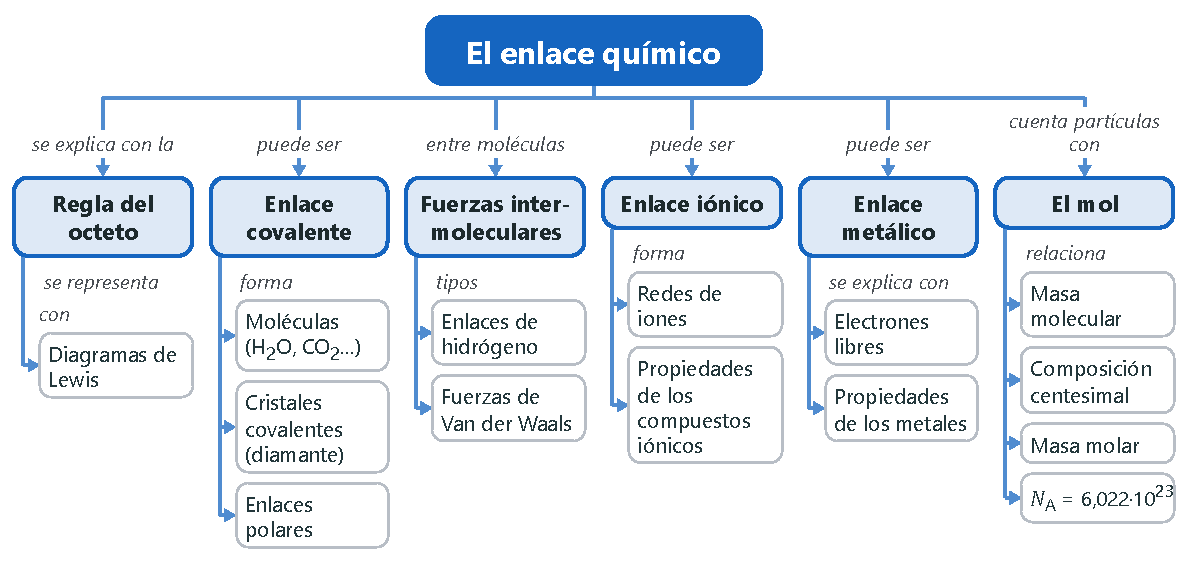
\includegraphics[width=\textwidth]{images/mapas_conceptuales/mapa_UD3}
\end{figure}

%========================================================================================
%\section*{Para empezar: las formas alotrópicas del carbono}
%\addcontentsline{toc}{section}{Para empezar: las formas alotrópicas del carbono}
%========================================================================================
%
%Hablamos de \textbf{alotropía} cuando un mismo elemento, en el mismo estado físico, se presenta en variedades distintas con propiedades físicas y químicas diferentes. Le ocurre a muchos metales y no metales, pero el ejemplo más famoso es el carbono. En la naturaleza aparece como \textbf{grafito} (la mina de los lápices) y como \textbf{diamante}, y en el laboratorio se han obtenido otras formas sorprendentes (figura~\ref{fig:alotropos_carbono}):
%
%\begin{itemize}
%    \item Los \textbf{fullerenos} son «jaulas» de entre 28 y \num{1500} átomos de carbono. Los más conocidos son las \emph{bucky balls}, esferas de 60 átomos con forma de balón de fútbol. Los \textbf{nanotubos} también son fullerenos, con forma de tubo. Tienen propiedades semiconductoras y superconductoras, por lo que interesan a las industrias electrónica, óptica y biomédica; además, por su forma y por ser compatibles con el organismo, pueden transportar fármacos dentro del cuerpo.
%    \item El \textbf{grafeno} es una lámina plana de átomos de carbono colocados en forma de panal de abejas. Como tiene solo un átomo de espesor, se considera un material \textbf{bidimensional}. Es transparente y conduce el calor y la electricidad mejor que el silicio, por lo que podría sustituirlo en la electrónica del futuro.
%\end{itemize}
%
%\begin{figure}[H]
%    \centering
%    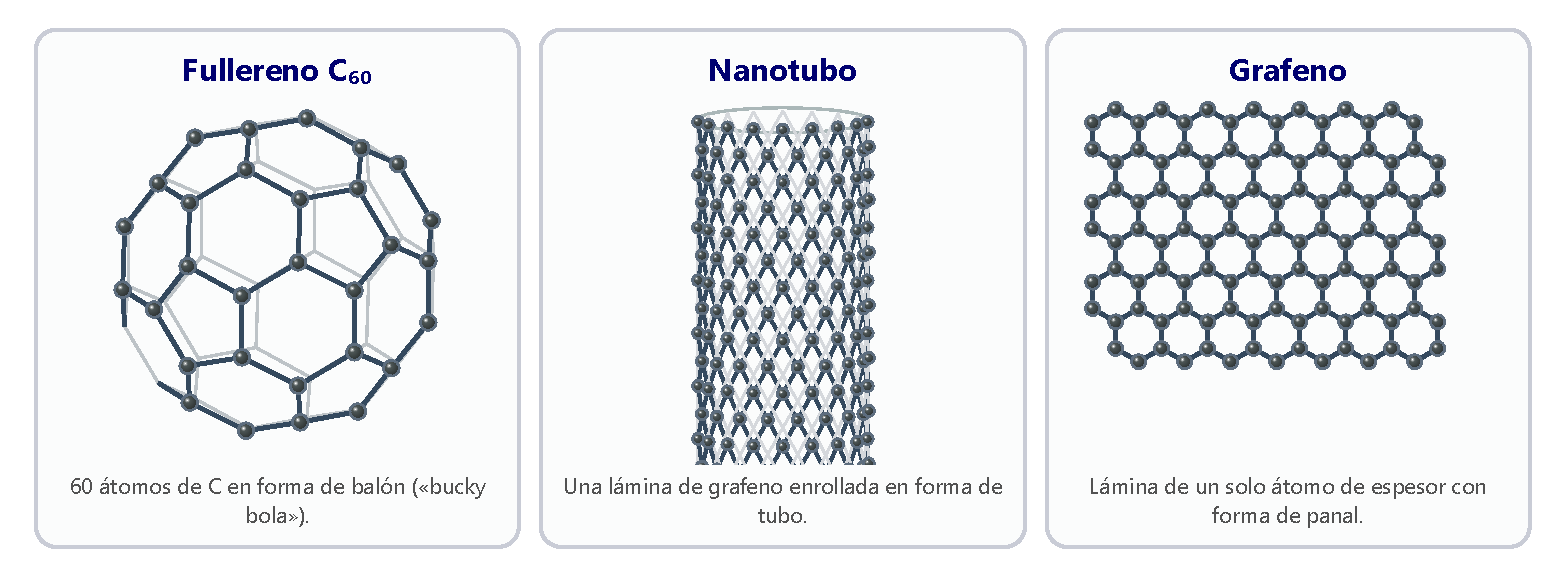
\includegraphics[width=\textwidth]{images/UD3/alotropos_carbono}
%    \caption{Algunas formas alotrópicas del carbono obtenidas en el laboratorio.}
%    \label{fig:alotropos_carbono}
%\end{figure}
%
%\begin{remark}
%    \textbf{Carbono y Objetivos de Desarrollo Sostenible.} Los fullerenos se usan en la industria farmacéutica para transportar medicamentos (\textbf{ODS 3}, \emph{Salud y bienestar}), y el grafeno se investiga para fabricar dispositivos electrónicos y gestionar mejor la energía (\textbf{ODS 7}, \emph{Energía asequible y no contaminante}). Al ser el carbono un elemento muy abundante, su uso no tiene por qué amenazar los recursos naturales.
%\end{remark}
%
%\begin{exercise}
%    Explica con tus palabras qué es la alotropía. ¿Qué formas alotrópicas del carbono se encuentran en la naturaleza y cuáles se han fabricado en el laboratorio?
%    \begin{solu}
%        La alotropía es la existencia de variedades distintas de un mismo elemento, en el mismo estado físico, con propiedades físicas y químicas diferentes. En la naturaleza el carbono aparece como \textcolor{red}{grafito y diamante}; en el laboratorio se han obtenido los \textcolor{red}{fullerenos} (como las \emph{bucky balls}), los \textcolor{red}{nanotubos} y el \textcolor{red}{grafeno}.
%    \end{solu}
%\end{exercise}
%
%\begin{exercise}
%    ¿Cuántos átomos forman los fullerenos? ¿Por qué resultan útiles en medicina? ¿Y en la industria electrónica y óptica?
%    \begin{solu}
%        Están formados por entre 28 y \num{1500} átomos de carbono. Por su estructura y su biocompatibilidad pueden \textcolor{red}{transportar fármacos} dentro del organismo. En electrónica y óptica interesan porque tienen propiedades \textcolor{red}{semiconductoras y superconductoras}.
%    \end{solu}
%\end{exercise}
%
%\begin{exercise}
%    ¿Qué es el grafeno? ¿Por qué se dice que es un material bidimensional? ¿Qué propiedad lo convierte en candidato para sustituir al silicio?
%    \begin{solu}
%        Es una lámina plana de átomos de carbono dispuestos en forma de panal. Es bidimensional porque tiene \textcolor{red}{un solo átomo de espesor}. Podría sustituir al silicio porque su \textcolor{red}{conductividad eléctrica es mayor} (y además es transparente).
%    \end{solu}
%\end{exercise}
%
%\begin{exercise}
%    ¿Crees que el uso de las formas alotrópicas del carbono supone una amenaza para el medioambiente? ¿Con qué Objetivos de Desarrollo Sostenible se relacionan?
%    \begin{solu}
%        En principio no, porque el carbono es un elemento abundante y sus aplicaciones no tienen por qué dañar el medio natural. Se relacionan con el \textcolor{red}{ODS 3} (transporte de fármacos) y con el \textcolor{red}{ODS 7} (electrónica y gestión de la energía).
%    \end{solu}
%\end{exercise}

%========================================================================================
\section{¿Por qué se unen los átomos? El enlace químico}
%========================================================================================

¿Por qué el helio o el neón se encuentran en la naturaleza como átomos sueltos, mientras que el oxígeno aparece en forma de moléculas, \ch{O2}? La respuesta está en los \textbf{electrones del último nivel}.

Los gases nobles tienen su último nivel \textbf{completo}: ocho electrones, con configuración \conf{ns^2~np^6}, salvo el helio, que tiene dos (\conf{1s^2}). Esta es la configuración electrónica más estable posible, por eso los gases nobles no se combinan de forma natural con otros elementos y aparecen como \textbf{átomos aislados}. El resto de los elementos se unen entre sí para conseguir una configuración como la del gas noble más próximo en la tabla periódica: esto explica su comportamiento químico.

\subsection{Los diagramas de Lewis y la regla del octeto}

\begin{definition}[Diagrama de Lewis]
    El \textbf{diagrama de Lewis} de un átomo es una forma de representar sus \textbf{electrones de valencia}, es decir, los de su último nivel. Se escribe el símbolo del elemento rodeado de tantos puntos (o aspas) como electrones de valencia tiene.
\end{definition}

\begin{figure}[H]
    \centering
    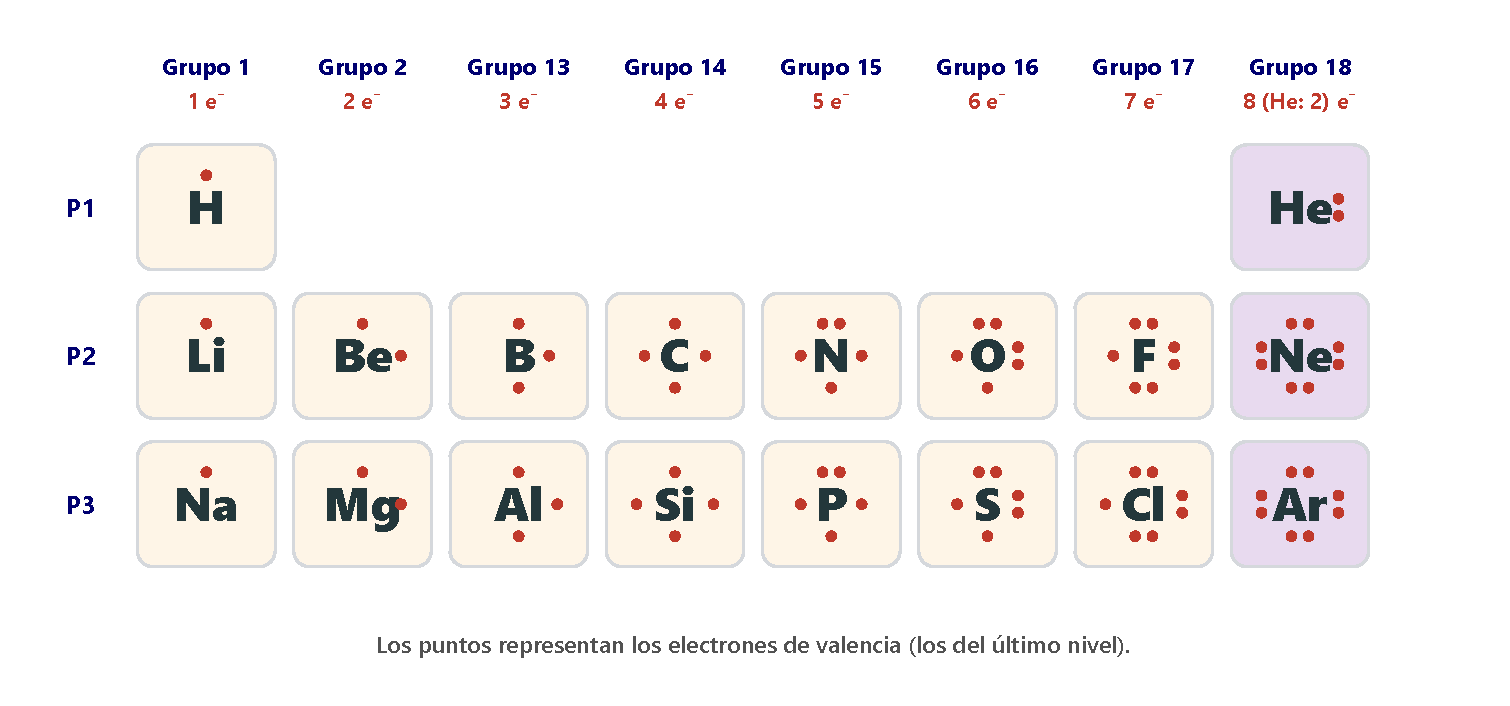
\includegraphics[width=0.9\textwidth]{images/UD3/lewis_tabla}
    \caption{Diagramas de Lewis de los elementos representativos de los tres primeros períodos.}
    \label{fig:lewis_tabla}
\end{figure}

En la figura~\ref{fig:lewis_tabla} se ve, por ejemplo, que al oxígeno le faltan \textbf{dos electrones} para tener ocho, como el neón, mientras que si el litio \textbf{pierde un electrón} se queda con la configuración del helio.

\begin{definition}[Regla del octeto]
    Los átomos tienden a ganar, perder o compartir electrones hasta tener \textbf{ocho electrones en su último nivel} (dos en el caso de los que se acercan al helio), igual que los gases nobles. Esta regla se cumple, sobre todo, en los elementos representativos.
\end{definition}

\begin{exercise}
    Investiga sobre las propiedades físicas y químicas de los gases nobles. ¿Por qué se presentan en la naturaleza como átomos aislados?
    \begin{solu}
        Respuesta libre. Son gases incoloros e inodoros, con puntos de fusión y ebullición muy bajos, y prácticamente no reaccionan con otras sustancias. Se presentan como átomos aislados porque su \textcolor{red}{último nivel está completo} (ocho electrones, o dos en el helio), que es la configuración más estable.
    \end{solu}
\end{exercise}

\begin{exercise}
    Dibuja los diagramas de Lewis de estos elementos: Mg (\(Z = 12\)), Al (\(Z = 13\)), Si (\(Z = 14\)), P (\(Z = 15\)), S (\(Z = 16\)) y Cl (\(Z = 17\)).
    \begin{solu}
        \textcolor{blue}{Todos están en el período 3; sus electrones de valencia son los del nivel 3 (2, 3, 4, 5, 6 y 7, respectivamente):}
        \begin{center}
            \chemfig{\charge{90=\.,0=\.}{Mg}} \qquad
            \chemfig{\charge{90=\.,0=\.,270=\.}{Al}} \qquad
            \chemfig{\charge{90=\.,0=\.,270=\.,180=\.}{Si}} \qquad
            \chemfig{\charge{90=\:,0=\.,270=\.,180=\.}{P}} \qquad
            \chemfig{\charge{90=\:,0=\:,270=\.,180=\.}{S}} \qquad
            \chemfig{\charge{90=\:,0=\:,270=\:,180=\.}{Cl}}
        \end{center}
    \end{solu}
\end{exercise}

\begin{exercise}
    Según la regla del octeto, ¿cuántos electrones tiende a ganar o perder un átomo de\ldots
    \begin{enumerate}[label=\alph*)]
        \item nitrógeno?
        \item un elemento del grupo 17?
        \item calcio?
        \item aluminio?
    \end{enumerate}
    \begin{solu}
        a) El N tiene 5 electrones de valencia: tiende a \textcolor{red}{ganar 3}. b) Tiene 7: tiende a \textcolor{red}{ganar 1}. c) El Ca (grupo 2) tiene 2: tiende a \textcolor{red}{perder 2}. d) El Al (grupo 13) tiene 3: tiende a \textcolor{red}{perder 3}.
    \end{solu}
\end{exercise}

\begin{exercise}
    Haz una tabla con el número de electrones de valencia y el diagrama de Lewis de los elementos del período 2: Li, Be, B, C, N, O, F y Ne.
    \begin{solu}
        \begin{center}
            % --- tabla antigua ---
            % \begin{tblr}{colspec={lcccccccc}, hlines, vlines, row{1}={bg=ocre!85, fg=white, font=\bfseries}, cell{1}{1}={bg=ocre!85, fg=white}}
                % Elemento & Li & Be & B & C & N & O & F & Ne \\
                % Electrones de valencia & 1 & 2 & 3 & 4 & 5 & 6 & 7 & 8 \\
                % Lewis & \chemfig{\charge{90=\.}{Li}} & \chemfig{\charge{90=\.,0=\.}{Be}} & \chemfig{\charge{90=\.,0=\.,270=\.}{B}} & \chemfig{\charge{90=\.,0=\.,270=\.,180=\.}{C}} & \chemfig{\charge{90=\:,0=\.,270=\.,180=\.}{N}} & \chemfig{\charge{90=\:,0=\:,270=\.,180=\.}{O}} & \chemfig{\charge{90=\:,0=\:,270=\:,180=\.}{F}} & \chemfig{\charge{90=\:,0=\:,270=\:,180=\:}{Ne}} \\
            % \end{tblr}
            % --- tabla nueva ---
            \begin{tabular}{@{}lcccccccc@{}}
                \toprule
                \textbf{Elemento} & \textbf{Li} & \textbf{Be} & \textbf{B} & \textbf{C} & \textbf{N} & \textbf{O} & \textbf{F} & \textbf{Ne} \\
                \midrule
                Electrones de valencia & 1 & 2 & 3 & 4 & 5 & 6 & 7 & 8 \\[3pt]
                Lewis & \chemfig{\charge{90=\.}{Li}} & \chemfig{\charge{90=\.,0=\.}{Be}} & \chemfig{\charge{90=\.,0=\.,270=\.}{B}} & \chemfig{\charge{90=\.,0=\.,270=\.,180=\.}{C}} & \chemfig{\charge{90=\:,0=\.,270=\.,180=\.}{N}} & \chemfig{\charge{90=\:,0=\:,270=\.,180=\.}{O}} & \chemfig{\charge{90=\:,0=\:,270=\:,180=\.}{F}} & \chemfig{\charge{90=\:,0=\:,270=\:,180=\:}{Ne}} \\
                \bottomrule
            \end{tabular}
        \end{center}
    \end{solu}
\end{exercise}

\begin{exercise}
    Escribe la configuración electrónica y el diagrama de Lewis del potasio (\(Z = 19\)). ¿Le resulta más fácil alcanzar la configuración de un gas noble ganando o perdiendo electrones? ¿De qué gas noble se trata?
    \begin{solu}
        K: \conf{1s^2~2s^2~2p^6~3s^2~3p^6~4s^1}; Lewis: \chemfig{\charge{90=\.}{K}}. Tiene un solo electrón de valencia, así que le resulta mucho más fácil \textcolor{red}{perderlo} que ganar siete. Así adquiere la configuración del \textcolor{red}{argón}.
    \end{solu}
\end{exercise}

\begin{exercise}
    Indica si son verdaderas o falsas estas afirmaciones y corrige las falsas:
    \begin{enumerate}[label=\alph*)]
        \item Todos los gases nobles tienen ocho electrones en su último nivel.
        \item Hay un elemento del grupo 18 con solo dos electrones en su último nivel.
        \item Algunos gases nobles son sólidos a temperatura ambiente.
        \item Los gases nobles se encuentran en la naturaleza como átomos aislados.
    \end{enumerate}
    \begin{solu}
        a) \textcolor{red}{Falsa}: todos tienen ocho, salvo el helio, que tiene dos. b) \textcolor{red}{Verdadera}: el helio. c) \textcolor{red}{Falsa}: todos los elementos del grupo 18 son gases a temperatura ambiente. d) \textcolor{red}{Verdadera}.
    \end{solu}
\end{exercise}

\begin{exercise}
    Un compañero ha dibujado estos diagramas de Lewis de átomos en su estado fundamental. ¿Cuáles son incorrectos? Escríbelos todos correctamente.
    \begin{center}
        \chemfig{\charge{90=\.,0=\.,180=\.}{Ca}} \qquad
        \chemfig{\charge{90=\:,0=\.,270=\.}{O}} \qquad
        \chemfig{\charge{90=\.,0=\.,270=\.,180=\.}{C}} \qquad
        \chemfig{\charge{90=\:,0=\:,270=\:}{Cl}} \qquad
        \chemfig{\charge{90=\:,0=\.,270=\.,180=\.}{N}}
    \end{center}
    \begin{solu}
        \textcolor{blue}{Contamos los electrones de valencia: Ca 2, O 6, C 4, Cl 7, N 5.} Son incorrectos los del \textcolor{red}{calcio} (tiene 3 puntos en lugar de 2), el \textcolor{red}{oxígeno} (4 en lugar de 6) y el \textcolor{red}{cloro} (6 en lugar de 7). Los correctos son:
        \begin{center}
            \chemfig{\charge{90=\.,0=\.}{Ca}} \qquad
            \chemfig{\charge{90=\:,0=\:,270=\.,180=\.}{O}} \qquad
            \chemfig{\charge{90=\.,0=\.,270=\.,180=\.}{C}} \qquad
            \chemfig{\charge{90=\:,0=\:,270=\:,180=\.}{Cl}} \qquad
            \chemfig{\charge{90=\:,0=\.,270=\.,180=\.}{N}}
        \end{center}
    \end{solu}
\end{exercise}

\subsection{¿Qué es un enlace químico?}

\begin{definition}[Enlace químico]
    Un \textbf{enlace químico} es la fuerza de tipo \textbf{electrostático} que mantiene unidos a los átomos en un elemento o en un compuesto.
\end{definition}

Veámoslo con la molécula más sencilla, la de hidrógeno, \ch{H2} (figura~\ref{fig:fuerzas_h2}). Cuando dos átomos de hidrógeno se acercan aparecen varias fuerzas:

\begin{itemize}
    \item Los dos \textbf{núcleos}, ambos positivos, \textbf{se repelen}.
    \item Los dos \textbf{electrones}, ambos negativos, también \textbf{se repelen}.
    \item Cada núcleo \textbf{atrae} a los dos electrones (el suyo y el del otro átomo).
\end{itemize}

El enlace se forma cuando las fuerzas de \textbf{atracción} superan a las de \textbf{repulsión}: los átomos quedan unidos a una distancia en la que el sistema es más estable que cuando estaban separados.

\begin{figure}[H]
    \centering
    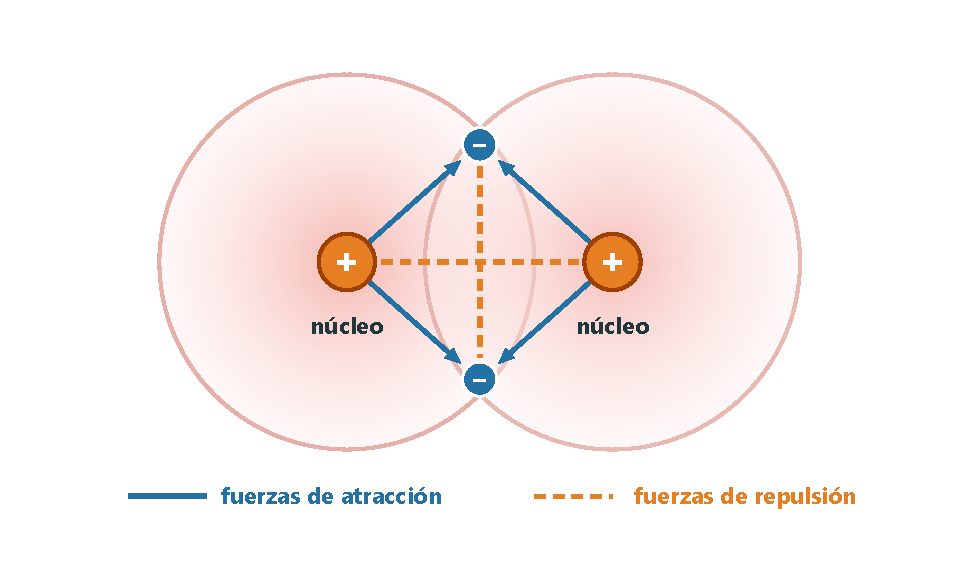
\includegraphics[width=0.55\textwidth]{images/UD3/fuerzas_h2}
    \caption{Fuerzas de atracción y de repulsión entre los núcleos y los electrones de dos átomos de hidrógeno.}
    \label{fig:fuerzas_h2}
\end{figure}

\begin{exercise}
    Define con tus palabras qué es un enlace químico.
    \begin{solu}
        Es la \textcolor{red}{fuerza de tipo electrostático} que mantiene unidos a los átomos dentro de un elemento o de un compuesto.
    \end{solu}
\end{exercise}

\begin{exercise}
    Haz en tu cuaderno un esquema de dos átomos de hidrógeno unidos y señala en él todas las fuerzas de atracción y de repulsión entre núcleos y electrones. ¿Qué condición se tiene que cumplir para que se forme el enlace?
    \begin{solu}
        Como en la figura~\ref{fig:fuerzas_h2}: \textcolor{blue}{repulsión} núcleo--núcleo y electrón--electrón; \textcolor{blue}{atracción} de cada núcleo sobre los dos electrones. El enlace se forma cuando las \textcolor{red}{fuerzas de atracción contrarrestan a las de repulsión}.
    \end{solu}
\end{exercise}

%========================================================================================
\section{El enlace covalente en elementos y compuestos}
%========================================================================================

\begin{definition}[Enlace covalente]
    Los átomos que consiguen su estabilidad \textbf{compartiendo electrones} con otros átomos están unidos mediante \textbf{enlaces covalentes}. Se da entre átomos de \textbf{no metales}. Cada par de electrones compartidos es un enlace.
\end{definition}

\subsection{Elementos covalentes moleculares}

El hidrógeno, el nitrógeno, el oxígeno y los halógenos (flúor, cloro, bromo y yodo) forman \textbf{moléculas diatómicas}: \ch{H2}, \ch{N2}, \ch{O2}, \ch{F2}, \ch{Cl2}, \ch{Br2}, \ch{I2}. Otros, como el fósforo (\ch{P4}) o el azufre (\ch{S8}), forman moléculas de más átomos. Según los electrones que compartan, el enlace puede ser sencillo, doble o triple (figura~\ref{fig:enlaces_f2_o2_n2}):

\begin{itemize}
    \item \textbf{Flúor, \ch{F2}: enlace sencillo.} Cada átomo de flúor (\conf{1s^2~2s^2~2p^5}) tiene 7 electrones de valencia y le falta uno. Los dos átomos comparten \textbf{un par} de electrones y cada uno queda rodeado de ocho.
    \item \textbf{Oxígeno, \ch{O2}: enlace doble.} Cada oxígeno (\conf{1s^2~2s^2~2p^4}) tiene 6 electrones de valencia y le faltan dos, así que los átomos comparten \textbf{dos pares}.
    \item \textbf{Nitrógeno, \ch{N2}: enlace triple.} Cada nitrógeno (\conf{1s^2~2s^2~2p^3}) tiene 5 electrones de valencia y le faltan tres: comparten \textbf{tres pares}.
\end{itemize}

En los tres casos cada átomo acaba rodeado de ocho electrones, como el neón. En las fórmulas desarrolladas cada par compartido se dibuja como un guion: \chemfig{F-F}, \chemfig{O=O}, \chemfig{N~N}.

\begin{figure}[H]
    \centering
    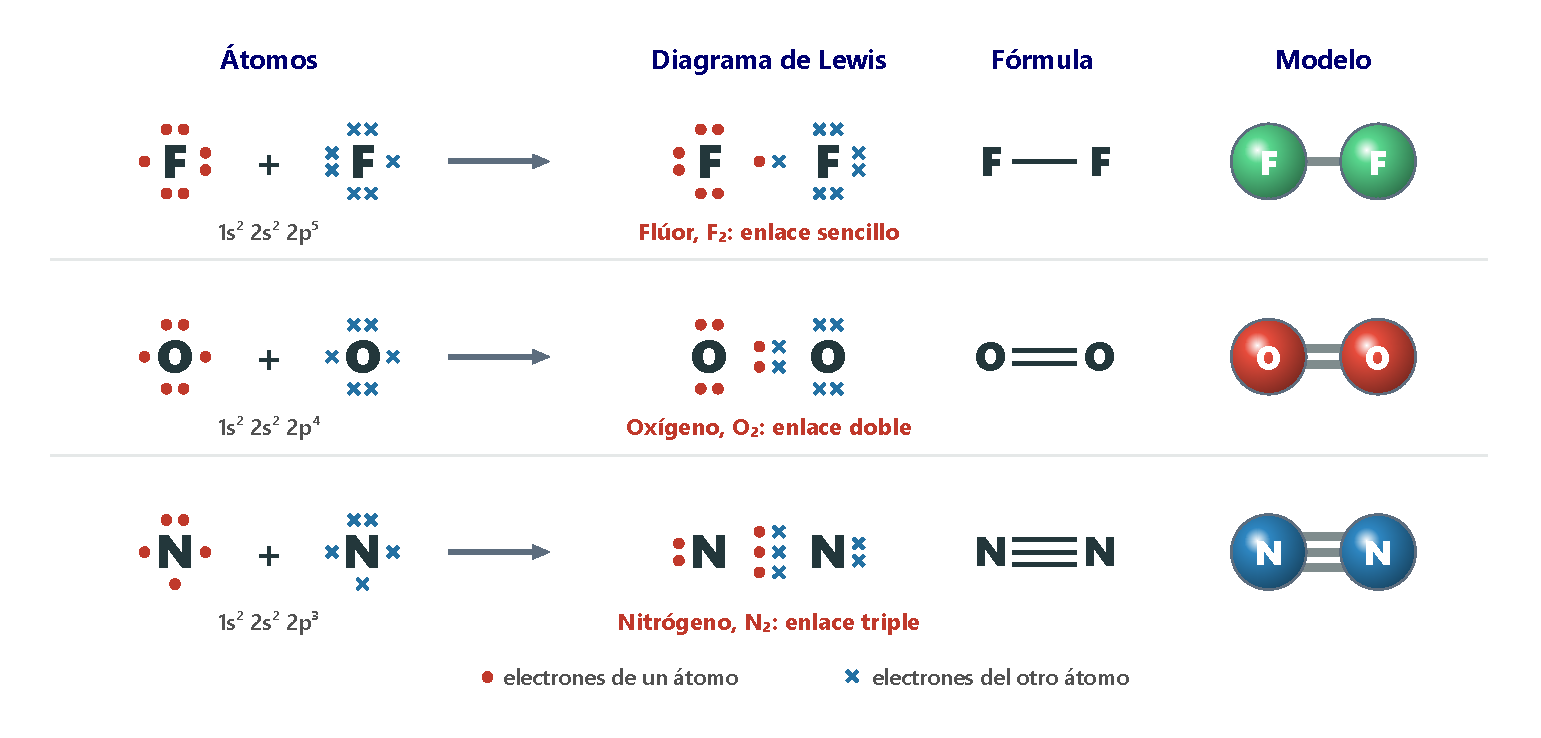
\includegraphics[width=\textwidth]{images/UD3/enlaces_f2_o2_n2}
    \caption{Formación de los enlaces sencillo, doble y triple en las moléculas de flúor, oxígeno y nitrógeno.}
    \label{fig:enlaces_f2_o2_n2}
\end{figure}

\paragraph{Propiedades de los elementos covalentes moleculares.} Suelen ser \textbf{gases} (\ch{H2}, \ch{O2}, \ch{N2}, \ch{F2}, \ch{Cl2}); el bromo es líquido y el yodo es un sólido que sublima con facilidad.
\begin{itemize}
    \item Tienen puntos de fusión y de ebullición \textbf{bajos}.
    \item \textbf{No conducen} la corriente eléctrica, porque no tienen electrones libres.
    \item Son \textbf{insolubles} o muy poco solubles en agua.
\end{itemize}

\begin{exercise}
    Fíjate en la figura~\ref{fig:enlaces_f2_o2_n2} y responde:
    \begin{enumerate}[label=\alph*)]
        \item ¿Cuántos electrones comparten los dos átomos en las moléculas de flúor, de oxígeno y de nitrógeno?
        \item ¿De cuántos electrones queda rodeado cada átomo?
        \item ¿Cuántos enlaces covalentes hay en cada molécula?
        \item ¿A qué gas noble se parecen así?
    \end{enumerate}
    \begin{solu}
        a) \ch{F2}: un par (2 electrones); \ch{O2}: dos pares (4 electrones); \ch{N2}: tres pares (6 electrones). b) De \textcolor{red}{ocho} electrones. c) \ch{F2}: \textcolor{red}{uno}; \ch{O2}: \textcolor{red}{dos}; \ch{N2}: \textcolor{red}{tres}. d) Al \textcolor{red}{neón}.
    \end{solu}
\end{exercise}

\begin{exercise}
    El bromo tiene número atómico \(Z = 35\).
    \begin{enumerate}[label=\alph*)]
        \item Escribe su configuración electrónica. ¿Cuántos electrones tiene en su último nivel?
        \item ¿Qué tipo de molécula forma? ¿Por qué?
        \item Representa con diagramas de Lewis cómo se forma la molécula.
    \end{enumerate}
    \begin{solu}
        a) \conf{1s^2~2s^2~2p^6~3s^2~3p^6~4s^2~3d^{10}~4p^5}. Tiene \textcolor{red}{7 electrones} en el último nivel (\(4s^2\,4p^5\)).
        b) Le falta un electrón para completar el octeto. Dos átomos de bromo comparten un par de electrones y forman una \textcolor{red}{molécula diatómica, \ch{Br2}}, con un enlace sencillo.
        c)
        \begin{center}
            \chemfig{\charge{90=\:,270=\:,180=\:,0=\.}{Br}} \(\;+\;\) \chemfig{\charge{90=\:,270=\:,0=\:,180=\.}{Br}} \(\;\longrightarrow\;\) \chemfig{\charge{90=\:,270=\:,180=\:}{Br}-\charge{90=\:,270=\:,0=\:}{Br}}
        \end{center}
    \end{solu}
\end{exercise}

\begin{exercise}
    Indica si el enlace entre los átomos de estas moléculas es sencillo, doble o triple: \ch{Cl2}, \ch{N2}, \ch{H2}, \ch{O2}, \ch{I2}. ¿Cuántos pares de electrones se comparten en cada una?
    \begin{solu}
        \ch{Cl2}: \textcolor{red}{sencillo} (1 par); \ch{N2}: \textcolor{red}{triple} (3 pares); \ch{H2}: \textcolor{red}{sencillo} (1 par); \ch{O2}: \textcolor{red}{doble} (2 pares); \ch{I2}: \textcolor{red}{sencillo} (1 par).
    \end{solu}
\end{exercise}

\begin{exercise}
    Dados los no metales neón, hidrógeno, bromo, carbono (diamante), nitrógeno, argón, carbono (grafito), oxígeno y cloro:
    \begin{enumerate}[label=\alph*)]
        \item Clasifícalos según se presenten en la naturaleza como átomos aislados, moléculas diatómicas o cristales covalentes.
        \item En las moléculas diatómicas, indica si el enlace es sencillo, doble o triple.
    \end{enumerate}
    \begin{solu}
        a) Átomos aislados: \textcolor{red}{neón y argón}. Moléculas diatómicas: \textcolor{red}{hidrógeno, bromo, nitrógeno, oxígeno y cloro}. Cristales covalentes: \textcolor{red}{diamante y grafito}.
        b) Sencillo: \ch{H2}, \ch{Br2} y \ch{Cl2}; doble: \ch{O2}; triple: \ch{N2}.
    \end{solu}
\end{exercise}

\subsection{Elementos en forma de cristales covalentes}

El carbono tiene puntos de fusión y ebullición muy altos, tanto en forma de grafito como de diamante, así que no puede estar formado por moléculas pequeñas. El átomo de carbono (\(Z = 6\), \conf{1s^2~2s^2~2p^2}) tiene cuatro electrones de valencia y le faltan cuatro: los consigue compartiendo un electrón con cada uno de \textbf{cuatro átomos de carbono} vecinos. Cada uno de estos, a su vez, se une a otros, y así sucesivamente, hasta formar una \textbf{red cristalina} gigante. A estas sustancias se les llama \textbf{cristales covalentes} o \textbf{sólidos reticulares}.

\begin{figure}[H]
    \centering
    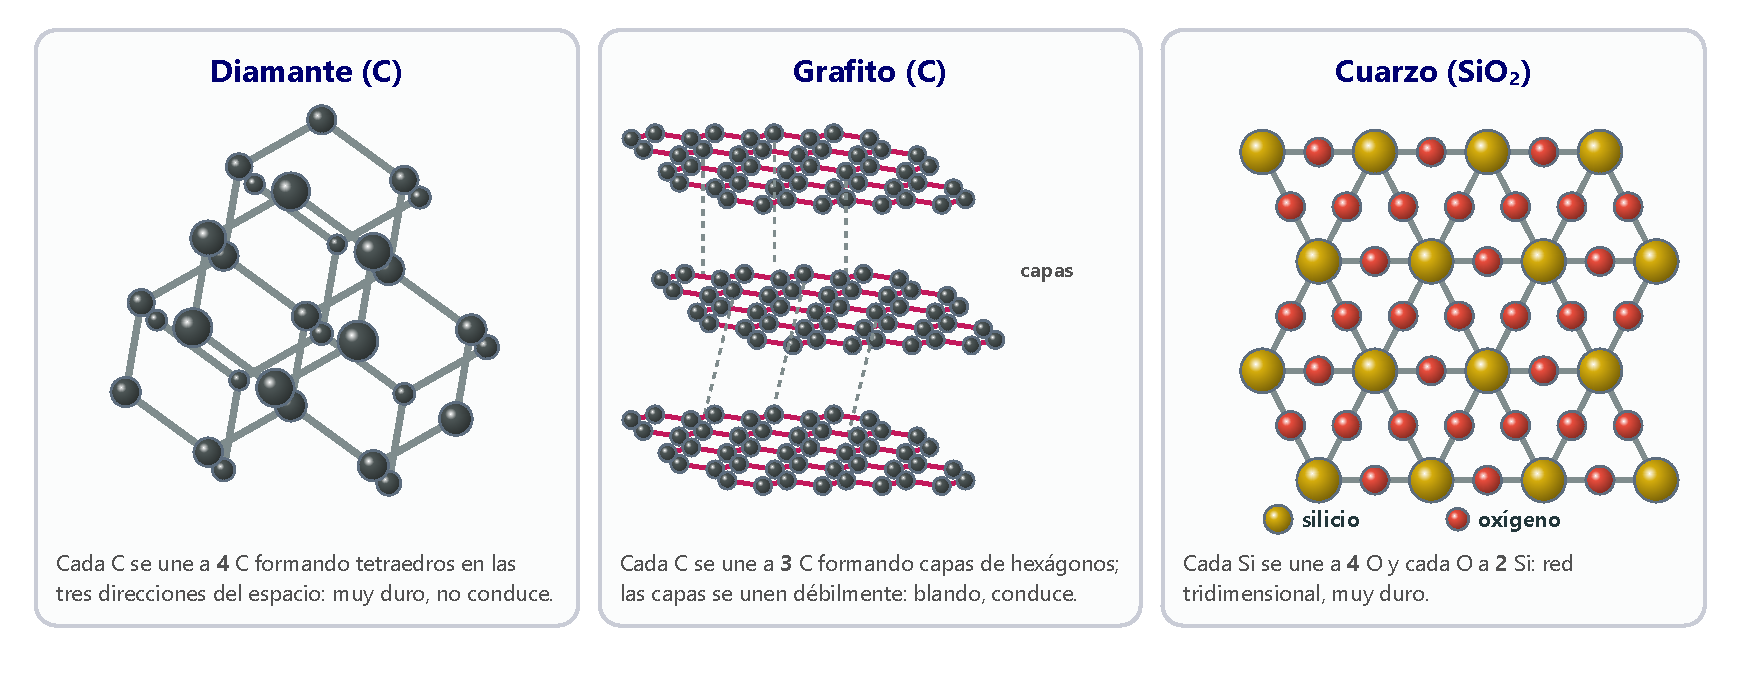
\includegraphics[width=\textwidth]{images/UD3/cristales_covalentes}
    \caption{Estructura de tres cristales covalentes: diamante, grafito y cuarzo.}
    \label{fig:cristales_covalentes}
\end{figure}

\begin{multicols}{2}
    \textbf{Diamante.} Cada átomo de carbono se une a otros \textbf{cuatro} formando tetraedros que se extienden en las tres direcciones del espacio. La red es muy fuerte: es una de las sustancias \textbf{más duras} que se conocen y sigue siendo sólida a temperaturas muy altas. Como todos los electrones están fijos en los enlaces, \textbf{no conduce} la corriente eléctrica.

    \columnbreak
    \textbf{Grafito.} Cada átomo de carbono se une fuertemente a otros \textbf{tres} de su mismo plano formando anillos de seis átomos. Las \textbf{capas} así formadas se unen entre sí débilmente y se deslizan unas sobre otras: el grafito es \textbf{blando}, negro y brillante. El cuarto electrón de cada carbono queda bastante libre, por eso el grafito \textbf{conduce} la electricidad.
\end{multicols}

\begin{exercise}
    ¿En qué se parecen y en qué se diferencian un cristal de diamante y uno de grafito?
    \begin{solu}
        \textcolor{blue}{Analogías:} los dos son cristales covalentes formados solo por átomos de carbono, tienen puntos de fusión muy altos y son insolubles en agua.
        \textcolor{blue}{Diferencias:} en el diamante cada C se une a 4 átomos en una red tridimensional; es muy duro y no conduce la electricidad. En el grafito cada C se une a 3 formando capas débilmente unidas; es blando, se exfolia en láminas y \textcolor{red}{conduce} la electricidad.
    \end{solu}
\end{exercise}

\begin{exercise}
    Los no metales pueden presentarse como átomos aislados, como moléculas o como cristales covalentes. Pon dos ejemplos de cada caso.
    \begin{solu}
        Respuesta libre. Por ejemplo: átomos aislados, \textcolor{red}{helio y argón}; moléculas, \textcolor{red}{\ch{O2} y \ch{Cl2}}; cristales covalentes, \textcolor{red}{diamante y grafito} (o silicio).
    \end{solu}
\end{exercise}

\begin{exercise}
    Dibuja el diagrama de Lewis de un átomo de silicio (\(Z = 14\)). ¿Por qué crees que el silicio forma cristales parecidos a los del diamante?
    \begin{solu}
        \chemfig{\charge{90=\.,0=\.,270=\.,180=\.}{Si}}. Como el carbono, tiene \textcolor{red}{4 electrones de valencia}, de modo que completa su octeto compartiendo un electrón con cada uno de cuatro átomos vecinos, lo que da lugar a una red tridimensional.
    \end{solu}
\end{exercise}

\begin{exercise}
    Indica si cada propiedad corresponde al diamante, al grafito o a los dos:
    \begin{enumerate}[label=\alph*)]
        \item es un cristal covalente;
        \item no conduce la electricidad;
        \item es muy duro;
        \item conduce la corriente eléctrica;
        \item no se disuelve en agua;
        \item es blando.
    \end{enumerate}
    \begin{solu}
        a) \textcolor{red}{Los dos}. b) \textcolor{red}{Diamante}. c) \textcolor{red}{Diamante}. d) \textcolor{red}{Grafito}. e) \textcolor{red}{Los dos}. f) \textcolor{red}{Grafito}.
    \end{solu}
\end{exercise}

\begin{exercise}
    Tanto en la molécula de \ch{H2} como en el diamante los átomos están unidos por enlaces covalentes. ¿Por qué entonces el hidrógeno es un gas y el diamante un sólido muy duro?
    \begin{solu}
        Las moléculas de \ch{H2} son pequeñas y están \textcolor{red}{aisladas} unas de otras (entre ellas apenas hay atracción), por eso es un gas. El diamante es una \textcolor{red}{red gigante} en la que todos los átomos están unidos por enlaces covalentes; para fundirlo habría que romper muchísimos enlaces, por eso es sólido y muy duro.
    \end{solu}
\end{exercise}

\begin{exercise}
    Haz un dibujo de cómo se unen los átomos de carbono en el diamante y en el grafito, y úsalo para explicar por qué el diamante es tan duro mientras que el grafito es blando y se separa en capas.
    \begin{solu}
        Dibujo como el de la figura~\ref{fig:cristales_covalentes}. En el diamante cada carbono está unido a cuatro en las \textcolor{red}{tres direcciones del espacio}: para rayarlo hay que romper enlaces fuertes en todas las direcciones. En el grafito los enlaces fuertes solo están dentro de cada capa; \textcolor{red}{entre capas la unión es débil}, por eso se deslizan y se separan fácilmente.
    \end{solu}
\end{exercise}

\subsection{Compuestos covalentes moleculares}

Los átomos de \textbf{distintos} no metales también se unen compartiendo electrones y forman \textbf{moléculas covalentes}. Son ejemplos el agua, el cloruro de hidrógeno, el amoníaco, el metano, el dióxido de carbono, el butano o el benceno (figura~\ref{fig:moleculas_covalentes}).

\begin{itemize}
    \item \textbf{Cloruro de hidrógeno, \ch{HCl}.} Al cloro (7 electrones de valencia) le falta uno para parecerse al argón y al hidrógeno (1 electrón) le falta otro para parecerse al helio. Comparten un par de electrones y quedan unidos por un \textbf{enlace sencillo}. La molécula es \textbf{lineal}.
    \item \textbf{Amoníaco, \ch{NH3}.} Al nitrógeno (5 electrones de valencia) le faltan tres. Forma tres enlaces sencillos, uno con cada átomo de hidrógeno, y le queda un par de electrones sin compartir. La molécula tiene forma de \textbf{pirámide}.
\end{itemize}

\begin{figure}[H]
    \centering
    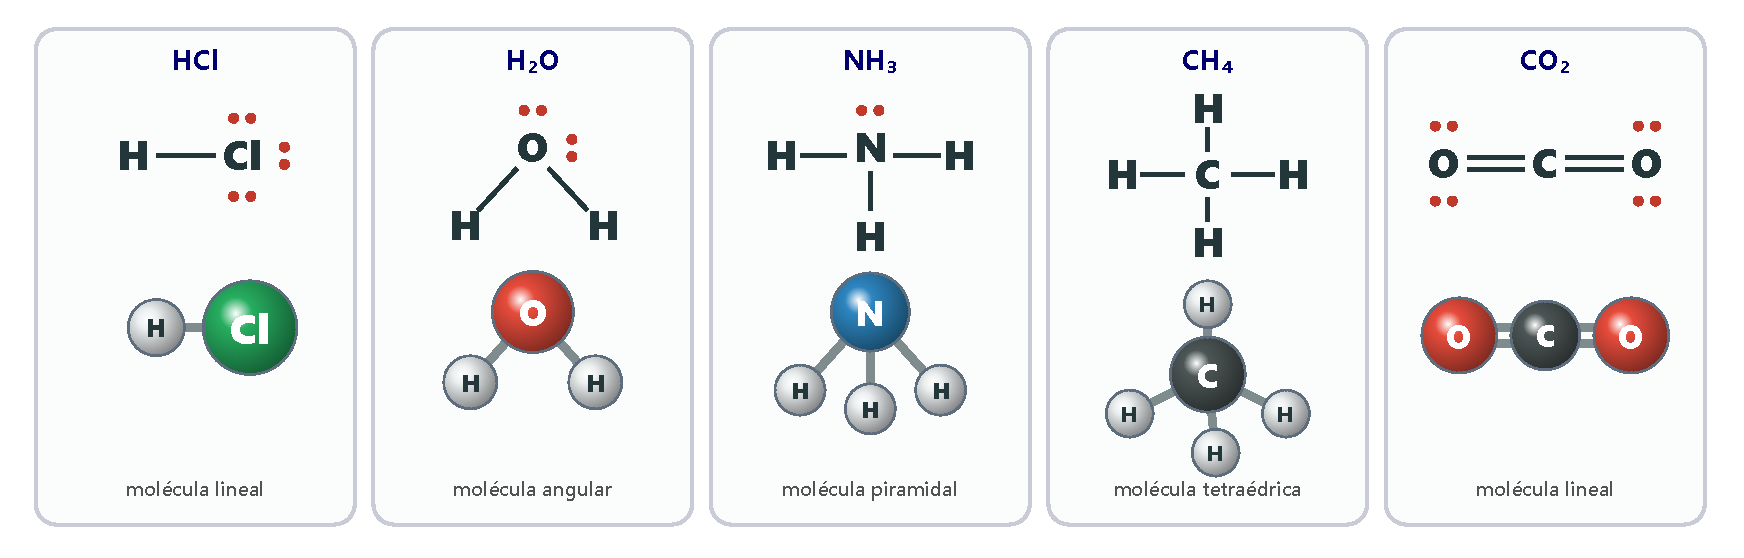
\includegraphics[width=\textwidth]{images/UD3/moleculas_covalentes}
    \caption{Diagramas de Lewis, fórmulas desarrolladas y modelos de bolas de algunas moléculas covalentes. Los puntos rojos son los pares de electrones sin compartir.}
    \label{fig:moleculas_covalentes}
\end{figure}

\paragraph{Propiedades de los compuestos covalentes moleculares.} Pueden ser gases, líquidos o sólidos; los sólidos son frágiles o blandos, como la cera.
\begin{itemize}
    \item Tienen puntos de fusión y ebullición \textbf{bajos}.
    \item Generalmente \textbf{no se disuelven en agua}, pero sí en disolventes como el benceno, el tolueno o la acetona.
    \item \textbf{No conducen} la electricidad.
\end{itemize}

\begin{exercise}
    Observa las propiedades de estas sustancias covalentes moleculares:
    \begin{center}
        % --- tabla antigua ---
        % \begin{tblr}{width=\linewidth, colspec={X[1.3,l]X[c]X[c]X[c]X[1.2,c]X[c]}, cells={font=\small}, hlines, vlines, row{1}={bg=ocre!85, fg=white, font=\small\bfseries}, column{1}={bg=ocre!15, font=\small\bfseries}, cell{1}{1}={bg=ocre!85, fg=white}, rowsep=1pt}
            % & Amoníaco, \ch{NH3} & Metano, \ch{CH4} & Benceno, \ch{C6H6} & Tetracloruro de carbono, \ch{CCl4} & Naftaleno, \ch{C10H8} \\
            % Aspecto & gas incoloro & gas incoloro & líquido incoloro & líquido incoloro & cristales en láminas \\
            % \(T_\text{f}\) (\unit{\celsius}) & \num{-78} & \num{-182} & \num{5.5} & \num{-23} & \num{80} \\
            % \(T_\text{e}\) (\unit{\celsius}) & \num{-33} & \num{-161} & \num{80} & \num{77} & \num{218} \\
            % ¿Conduce? & no & no & no & no & no \\
            % ¿Soluble en agua? & sí & no & no & no & no \\
        % \end{tblr}
        % --- tabla nueva ---
        {\small
        \begin{tabular}{@{}L{0.16\linewidth} c c c C{0.14\linewidth} c@{}}
            \toprule
             & \textbf{Amoníaco, \ch{NH3}} & \textbf{Metano, \ch{CH4}} & \textbf{Benceno, \ch{C6H6}} & \textbf{Tetracloruro de carbono, \ch{CCl4}} & \textbf{Naftaleno, \ch{C10H8}} \\
            \midrule
            \textbf{Aspecto} & gas incoloro & gas incoloro & líquido incoloro & líquido incoloro & cristales en láminas \\[3pt]
            \textbf{\(T_\text{f}\) (\unit{\celsius})} & \num{-78} & \num{-182} & \num{5.5} & \num{-23} & \num{80} \\[3pt]
            \textbf{\(T_\text{e}\) (\unit{\celsius})} & \num{-33} & \num{-161} & \num{80} & \num{77} & \num{218} \\[3pt]
            \textbf{¿Conduce?} & no & no & no & no & no \\[3pt]
            \textbf{¿Soluble en agua?} & sí & no & no & no & no \\
            \bottomrule
        \end{tabular}
        }
    \end{center}
    \begin{enumerate}[label=\alph*)]
        \item ¿Cómo son sus puntos de fusión y ebullición?
        \item ¿En qué estado están a \qty{25}{\celsius}?
        \item ¿Conducen la electricidad?
        \item ¿Son solubles en agua?
        \item ¿Qué propiedades tienen en común?
    \end{enumerate}
    \begin{solu}
        a) Son \textcolor{red}{bajos}. b) A \qty{25}{\celsius}, el amoníaco y el metano son \textcolor{red}{gases} (\(T_\text{e} < \qty{25}{\celsius}\)); el benceno y el tetracloruro de carbono son \textcolor{red}{líquidos} (\(T_\text{f} < \qty{25}{\celsius} < T_\text{e}\)) y el naftaleno es \textcolor{red}{sólido} (\(T_\text{f} > \qty{25}{\celsius}\)). c) \textcolor{red}{No}. d) Salvo el amoníaco, \textcolor{red}{no}. e) Puntos de fusión y ebullición bajos, no conducen la electricidad y casi todas son insolubles en agua.
    \end{solu}
\end{exercise}

\begin{exercise}
    Dibuja los diagramas de Lewis de: \ch{H2}, \ch{HBr}, \ch{F2}, \ch{CH4}, \ch{O2}, \ch{HF}, \ch{H2O}, \ch{NH3} y \ch{H2S}.
    \begin{solu}
        \begin{center}
            \chemfig{H-H} \qquad
            \chemfig{H-\charge{90=\:,0=\:,270=\:}{Br}} \qquad
            \chemfig{\charge{90=\:,180=\:,270=\:}{F}-\charge{90=\:,0=\:,270=\:}{F}} \qquad
            \chemfig{C(-[2]H)(-[4]H)(-[6]H)-H} \qquad
            \chemfig{\charge{90=\:,180=\:}{O}=\charge{90=\:,0=\:}{O}}

            \medskip
            \chemfig{H-\charge{90=\:,0=\:,270=\:}{F}} \qquad
            \chemfig{H-\charge{90=\:,270=\:}{O}-H} \qquad
            \chemfig{H-\charge{90=\:}{N}(-[6]H)-H} \qquad
            \chemfig{H-\charge{90=\:,270=\:}{S}-H}
        \end{center}
    \end{solu}
\end{exercise}

\begin{exercise}
    Interpreta estos diagramas de Lewis: ¿cuántos electrones de valencia tiene cada átomo y qué tipo de enlaces se forman?
    \begin{center}
        \chemfig{\charge{90=\:,270=\:}{O}=C=\charge{90=\:,270=\:}{O}} \qquad
        \chemfig{\charge{180=\:}{N}~\charge{0=\:}{N}} \qquad
        \chemfig{H-\charge{90=\:,270=\:}{Cl}}
    \end{center}
    \begin{solu}
        \textcolor{blue}{\ch{CO2}:} el carbono tiene 4 electrones de valencia y cada oxígeno 6. El carbono comparte dos pares con cada oxígeno: \textcolor{red}{dos enlaces dobles}.
        \textcolor{blue}{\ch{N2}:} cada nitrógeno tiene 5 electrones de valencia y comparte tres con el otro: \textcolor{red}{enlace triple}.
        \textcolor{blue}{\ch{HCl}:} el hidrógeno tiene 1 electrón de valencia y el cloro 7; comparten un par: \textcolor{red}{enlace sencillo}. (Al cloro le quedan tres pares sin compartir: falta uno en el dibujo.)
    \end{solu}
\end{exercise}

\begin{exercise}
    Escribe el diagrama de Lewis del \ch{CO2} y del \ch{N2} sabiendo que \(Z(\ch{C}) = 6\), \(Z(\ch{O}) = 8\) y \(Z(\ch{N}) = 7\).
    \begin{solu}
        \chemfig{\charge{90=\:,270=\:}{O}=C=\charge{90=\:,270=\:}{O}} \qquad \chemfig{\charge{180=\:}{N}~\charge{0=\:}{N}}
    \end{solu}
\end{exercise}

\begin{exercise}
    ¿Por qué se usan los plásticos, que son compuestos covalentes, para recubrir los cables eléctricos?
    \begin{solu}
        Porque los compuestos covalentes moleculares \textcolor{red}{no conducen la corriente eléctrica}: no tienen electrones libres ni iones que puedan moverse. Son buenos aislantes.
    \end{solu}
\end{exercise}

\begin{exercise}
    El sulfuro de hidrógeno, \ch{H2S}, está formado por dos no metales.
    \begin{enumerate}[label=\alph*)]
        \item ¿Qué tipo de enlace hay entre el hidrógeno y el azufre?
        \item ¿Qué propiedades esperas que tenga?
    \end{enumerate}
    \begin{solu}
        a) \textcolor{red}{Covalente}, porque los dos son no metales. b) Será un compuesto molecular: con puntos de fusión y ebullición bajos (de hecho es un gas a temperatura ambiente), poco soluble en agua y \textcolor{red}{no conductor} de la electricidad.
    \end{solu}
\end{exercise}

\begin{exercise}
    El azufre y el oxígeno forman varios compuestos (\ch{SO}, \ch{SO2}, \ch{SO3}), aunque los dos tienen tendencia a captar electrones. ¿Cómo se mantienen unidos sus átomos?
    \begin{solu}
        Como ninguno de los dos cede electrones, los átomos se mantienen unidos \textcolor{red}{compartiendo electrones}: mediante \textcolor{red}{enlaces covalentes}.
    \end{solu}
\end{exercise}

\begin{exercise}
    El germano, \ch{GeH4}, es un gas incoloro que funde a \qty{-165}{\celsius} y hierve a \qty{-88}{\celsius}; no conduce la electricidad y no se disuelve en agua.
    \begin{enumerate}[label=\alph*)]
        \item ¿Qué tipo de enlace tendrá?
        \item ¿Estará formado por moléculas o por cristales?
    \end{enumerate}
    \begin{solu}
        a) Por sus propiedades, el enlace es \textcolor{red}{covalente}. b) Por sus bajísimos puntos de fusión y ebullición, está formado por \textcolor{red}{moléculas}.
    \end{solu}
\end{exercise}

\subsection{Compuestos covalentes en forma de cristales}

Algunos compuestos covalentes, como el \textbf{dióxido de silicio}, \ch{SiO2} (cuarzo, el componente principal de la arena), o el carburo de silicio, \ch{SiC}, son muy duros y tienen puntos de fusión y ebullición muy altos. No están formados por moléculas, sino que son \textbf{redes cristalinas tridimensionales}: en el cuarzo, cada átomo de silicio se une a cuatro de oxígeno y cada oxígeno a dos de silicio (figura~\ref{fig:cristales_covalentes}).

\paragraph{Propiedades de los compuestos covalentes cristalinos.}
\begin{itemize}
    \item Puntos de fusión y ebullición \textbf{muy elevados}: el enlace covalente es muy fuerte y hay que romper muchos enlaces.
    \item Son \textbf{muy duros}: para rayarlos hay que destruir numerosos enlaces covalentes.
    \item \textbf{No conducen} la corriente eléctrica, porque no tienen electrones libres.
    \item \textbf{No se disuelven} en agua ni en otros disolventes.
\end{itemize}

\begin{exercise}
    Indica si cada propiedad corresponde a un compuesto covalente molecular, a uno reticular (cristalino) o a los dos:
    \begin{enumerate}[label=\alph*)]
        \item Puede ser gas, líquido o un sólido blando.
        \item Sólido muy duro.
        \item No conduce la electricidad.
        \item Puntos de fusión y ebullición muy altos.
        \item No se disuelve en agua, pero sí en acetona o tolueno.
        \item No se disuelve en ningún disolvente.
        \item Puntos de fusión y ebullición bajos.
    \end{enumerate}
    \begin{solu}
        a) Molecular. b) Reticular. c) \textcolor{red}{Los dos}. d) Reticular. e) Molecular. f) Reticular. g) Molecular.
    \end{solu}
\end{exercise}

\begin{exercise}
    Dada esta lista de sustancias: carbono (grafito), cuarzo, carbono (diamante), \ch{HBr}, \ch{Cl2}, \ch{Ne}, \ch{HCl}, \ch{Ar}, \ch{I2}, \ch{H2O}, \ch{CH4}, \ch{N2}.
    \begin{enumerate}[label=\alph*)]
        \item Separa los elementos de los compuestos.
        \item Clasifícalas en átomos aislados, moléculas covalentes y cristales covalentes.
        \item Cita dos elementos formados por moléculas diatómicas y dos elementos que no formen moléculas.
        \item Indica una sustancia que conduzca la electricidad y otra que no.
    \end{enumerate}
    \begin{solu}
        a) Elementos: grafito, diamante, \ch{Cl2}, \ch{Ne}, \ch{Ar}, \ch{I2}, \ch{N2}. Compuestos: cuarzo, \ch{HBr}, \ch{HCl}, \ch{H2O}, \ch{CH4}.
        b) Átomos aislados: \ch{Ne}, \ch{Ar}. Moléculas: \ch{HBr}, \ch{Cl2}, \ch{HCl}, \ch{I2}, \ch{H2O}, \ch{CH4}, \ch{N2}. Cristales covalentes: grafito, diamante y cuarzo.
        c) Por ejemplo, \ch{Cl2} y \ch{N2}; \ch{Ne} y el diamante.
        d) Conduce: \textcolor{red}{el grafito}; las demás \textcolor{red}{no conducen} (por ejemplo, el cuarzo).
    \end{solu}
\end{exercise}

\subsection{¿Puede haber cargas eléctricas en un enlace covalente?}

En el enlace covalente los electrones se comparten, pero no siempre a partes iguales:

\begin{itemize}
    \item \textbf{Enlace covalente apolar.} Si los dos átomos son \textbf{iguales} (\ch{Cl2}, \ch{H2}\ldots), atraen por igual a los electrones compartidos. El centro de las cargas positivas (núcleos) coincide con el de las negativas (electrones) y la molécula no tiene polos: es \textbf{apolar}.
    \item \textbf{Enlace covalente polar.} Si los átomos son \textbf{distintos}, uno suele atraer con más fuerza a los electrones compartidos. En el \ch{HCl}, el cloro atrae más a los electrones y adquiere una \textbf{carga parcial negativa} (\(\delta^-\)); el hidrógeno queda con una \textbf{carga parcial positiva} (\(\delta^+\)). La molécula es \textbf{polar}.
\end{itemize}

\begin{definition}[Dipolo]
    Un \textbf{dipolo} es una molécula polar, con un extremo cargado parcialmente positivo y otro negativo. Son dipolos el \ch{HCl}, el \ch{HF}, el \ch{H2O} y el \ch{NH3}: en el \ch{HF} el flúor soporta la carga negativa, y en el \ch{NH3}, el nitrógeno.
\end{definition}

\begin{figure}[H]
    \centering
    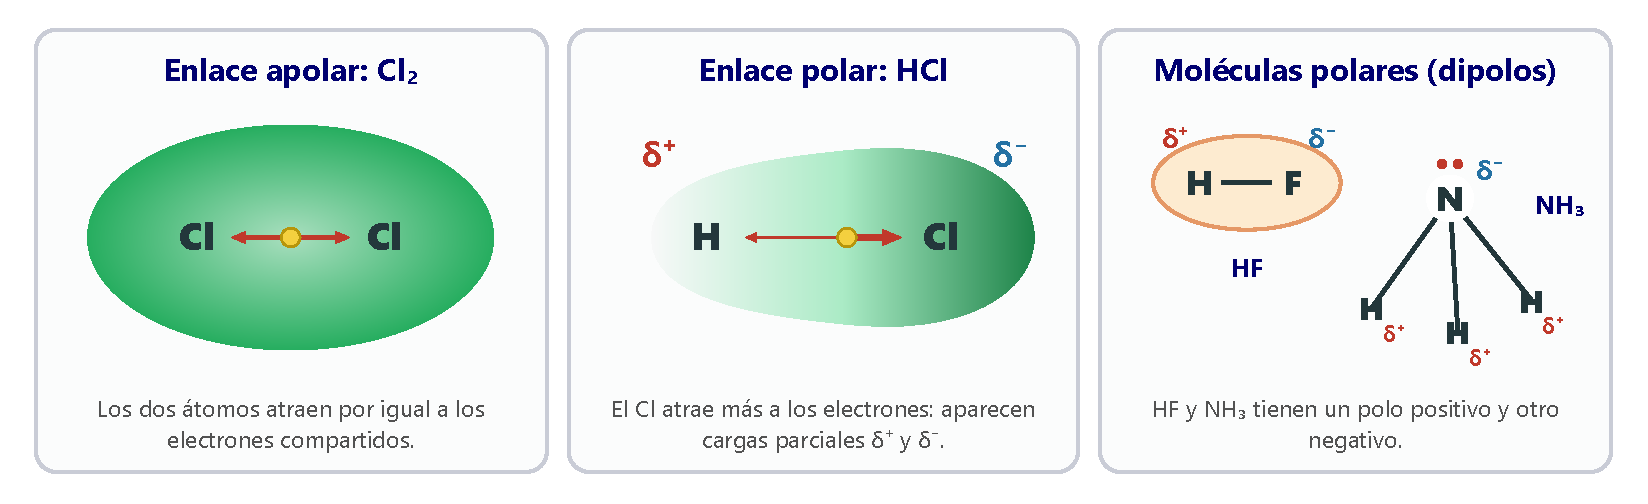
\includegraphics[width=\textwidth]{images/UD3/polaridad}
    \caption{Enlace apolar (\ch{Cl2}), enlace polar (\ch{HCl}) y moléculas polares o dipolos.}
    \label{fig:polaridad}
\end{figure}

\begin{exercise}
    Dibuja una molécula apolar de cloro, \ch{Cl2}, y una molécula polar de bromuro de hidrógeno, \ch{HBr}, indicando las cargas parciales.
    \begin{solu}
        \chemfig{Cl-Cl} (sin cargas parciales: los dos átomos atraen igual a los electrones). \qquad \chemfig{\overset{\delta^+}{\text{H}}-\overset{\delta^-}{\text{Br}}}: el bromo atrae más a los electrones del enlace y queda con la \textcolor{red}{carga parcial negativa}.
    \end{solu}
\end{exercise}

\begin{exercise}
    Corrige las afirmaciones falsas:
    \begin{enumerate}[label=\alph*)]
        \item Un enlace covalente es apolar cuando el centro de las cargas positivas no coincide con el de las negativas.
        \item Un enlace covalente es polar cuando los dos núcleos atraen por igual a los electrones compartidos.
        \item Un enlace covalente es polar cuando un extremo de la molécula tiene carga parcial positiva y el otro negativa.
        \item Un enlace covalente es apolar si uno de los átomos atrae con más fuerza a los electrones.
    \end{enumerate}
    \begin{solu}
        a) \textcolor{red}{Falsa}: es apolar cuando los dos centros \emph{coinciden}. b) \textcolor{red}{Falsa}: en ese caso es \emph{apolar}. c) \textcolor{red}{Verdadera}. d) \textcolor{red}{Falsa}: en ese caso es \emph{polar}.
    \end{solu}
\end{exercise}

%========================================================================================
\section{¿Pueden atraerse los dipolos? Las fuerzas intermoleculares}
%========================================================================================

Las moléculas polares pueden atraerse unas a otras: el extremo positivo de un dipolo atrae al extremo negativo de otro. Estas atracciones entre moléculas se llaman \textbf{fuerzas intermoleculares} y son de dos tipos:
\begin{itemize}
    \item Enlaces o fuerzas de \textbf{hidrógeno}.
    \item Fuerzas de \textbf{Van der Waals}.
\end{itemize}
Son mucho más débiles que los enlaces covalentes. Para distinguirlas, en los dibujos se representan con \textbf{líneas de puntos}.

\subsection{Enlaces o fuerzas de hidrógeno}

\begin{definition}[Enlace de hidrógeno]
    Es la atracción electrostática entre moléculas polares en las que el \textbf{hidrógeno} está unido a un átomo pequeño y con mucha tendencia a captar electrones: \textbf{flúor, oxígeno o nitrógeno}. El hidrógeno de una molécula (\(\delta^+\)) atrae al átomo de F, O o N (\(\delta^-\)) de una molécula vecina.
\end{definition}

\begin{figure}[H]
    \centering
    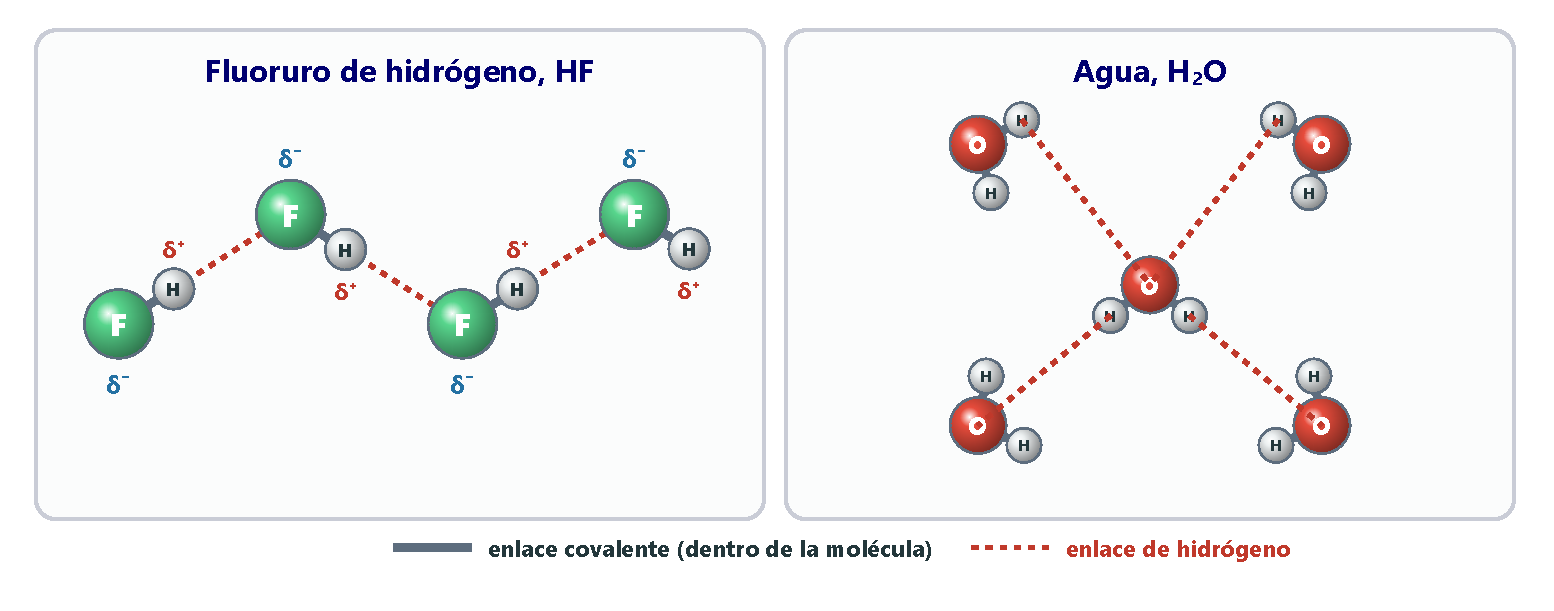
\includegraphics[width=0.85\textwidth]{images/UD3/enlace_hidrogeno}
    \caption{Enlaces de hidrógeno entre moléculas de fluoruro de hidrógeno y entre moléculas de agua.}
    \label{fig:enlace_hidrogeno}
\end{figure}

Estos enlaces mantienen unidas las moléculas de \ch{HF}, \ch{H2O} y \ch{NH3}, de modo que hace falta más energía para separarlas. Por eso sus puntos de fusión y ebullición son \textbf{anormalmente altos} si los comparamos con los de los hidruros de los demás elementos de su grupo (figura~\ref{fig:hidruros_ebullicion}). También hay enlaces de hidrógeno en sustancias como los alcoholes, las proteínas o el ADN.

\begin{figure}[H]
    \centering
    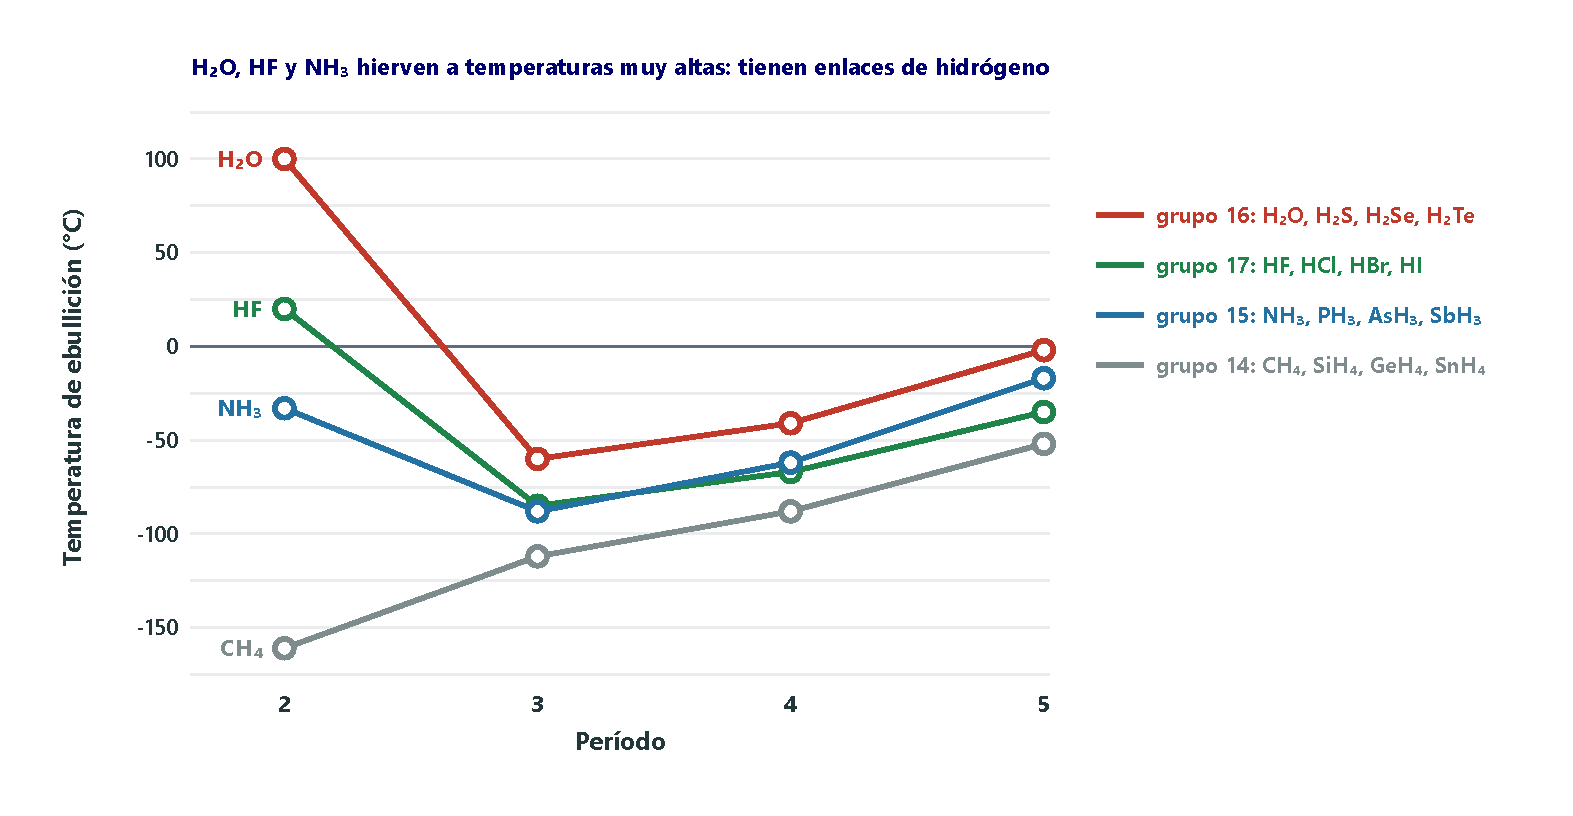
\includegraphics[width=0.9\textwidth]{images/UD3/hidruros_ebullicion}
    \caption{Temperaturas de ebullición de los hidruros de los grupos 14 a 17.}
    \label{fig:hidruros_ebullicion}
\end{figure}

\begin{exercise}
    Las proteínas y los ácidos nucleicos (como el ADN) son macromoléculas formadas sobre todo por carbono, hidrógeno, oxígeno y nitrógeno. Investiga y redacta un breve informe sobre el papel de los enlaces de hidrógeno en estas moléculas.
    \begin{solu}
        Respuesta libre. Por ejemplo: en el ADN, las dos cadenas de la doble hélice se mantienen unidas mediante enlaces de hidrógeno entre las bases nitrogenadas (A--T y G--C); en las proteínas, los enlaces de hidrógeno entre grupos \ch{N-H} y \ch{C=O} dan lugar a estructuras como la hélice \(\upalpha\) y la lámina \(\upbeta\).
    \end{solu}
\end{exercise}

\begin{exercise}
    Dibuja cómo se forman los enlaces de hidrógeno entre moléculas de fluoruro de hidrógeno. Explica por qué el \ch{HF} hierve a una temperatura mucho más alta que el resto de los hidruros del grupo 17.
    \begin{solu}
        \[ \cdots\,\overset{\delta^+}{\text{H}}\!-\!\overset{\delta^-}{\text{F}}\,\cdots\,\overset{\delta^+}{\text{H}}\!-\!\overset{\delta^-}{\text{F}}\,\cdots\,\overset{\delta^+}{\text{H}}\!-\!\overset{\delta^-}{\text{F}}\,\cdots \]
        (las líneas de puntos son los enlaces de hidrógeno; los guiones, los enlaces covalentes). Las moléculas de \ch{HF} no están aisladas: los enlaces de hidrógeno las mantienen unidas y hace falta \textcolor{red}{más energía para separarlas}. En \ch{HCl}, \ch{HBr} y \ch{HI} no hay enlaces de hidrógeno.
    \end{solu}
\end{exercise}

\begin{exercise}
    Dibuja los enlaces de hidrógeno entre moléculas de amoníaco, \ch{NH3}, y justifica por qué su temperatura de ebullición es mayor que la de los hidruros de los demás elementos del grupo 15.
    \begin{solu}
        El nitrógeno (\(\delta^-\)) de una molécula atrae a un hidrógeno (\(\delta^+\)) de la vecina:
        \[ \text{H}_2\overset{\delta^-}{\text{N}}\!-\!\overset{\delta^+}{\text{H}}\,\cdots\,\overset{\delta^-}{\text{N}}\text{H}_2\!-\!\overset{\delta^+}{\text{H}}\,\cdots\,\overset{\delta^-}{\text{N}}\text{H}_3 \]
        Su temperatura de ebullición es mayor porque en \ch{PH3}, \ch{AsH3} y \ch{SbH3} \textcolor{red}{no hay enlaces de hidrógeno}.
    \end{solu}
\end{exercise}

\begin{exercise}
    Analiza la gráfica de la figura~\ref{fig:hidruros_ebullicion} e indica tres hidruros con enlaces de hidrógeno entre sus moléculas y tres en los que no existan o sean muy débiles.
    \begin{solu}
        Con enlaces de hidrógeno: \textcolor{red}{\ch{H2O}, \ch{HF} y \ch{NH3}}, cuyas temperaturas de ebullición son mucho más altas de lo que les correspondería por su tamaño. Sin ellos: por ejemplo, \textcolor{red}{\ch{CH4}, \ch{SiH4} y \ch{GeH4}}.
    \end{solu}
\end{exercise}

\subsection{El agua, una molécula singular}

El oxígeno (\conf{1s^2~2s^2~2p^4}) tiene seis electrones de valencia y le faltan dos; por eso se une a \textbf{dos átomos de hidrógeno}, cada uno con un electrón, mediante dos enlaces covalentes sencillos \ch{O-H}. La molécula es \textbf{angular} y \textbf{polar}: el oxígeno atrae con más fuerza a los electrones y soporta la carga parcial negativa, y los hidrógenos, la positiva. Entre moléculas de agua se forman, por tanto, \textbf{enlaces de hidrógeno}.

\begin{center}
    % --- tabla antigua ---
    % \begin{tblr}{colspec={lcc}, hlines, vlines, row{1}={bg=ocre!85, fg=white, font=\bfseries}, column{1}={bg=ocre!15}, cell{1}{1}={bg=ocre!85, fg=white}}
        % Hidruros del grupo 16 & \(T_\text{f}\) (\unit{\celsius}) & \(T_\text{e}\) (\unit{\celsius}) \\
        % \ch{H2O} & \num{0} & \num{100} \\
        % \ch{H2S} & \num{-82} & \num{-60} \\
        % \ch{H2Se} & \num{-62} & \num{-41} \\
        % \ch{H2Te} & \num{-49} & \num{-1} \\
    % \end{tblr}
    % --- tabla nueva ---
    \begin{tabular}{@{}lcc@{}}
        \toprule
        \textbf{Hidruros del grupo 16} & \textbf{\(T_\text{f}\) (\unit{\celsius})} & \textbf{\(T_\text{e}\) (\unit{\celsius})} \\
        \midrule
        \ch{H2O} & \num{0} & \num{100} \\[3pt]
        \ch{H2S} & \num{-82} & \num{-60} \\[3pt]
        \ch{H2Se} & \num{-62} & \num{-41} \\[3pt]
        \ch{H2Te} & \num{-49} & \num{-1} \\
        \bottomrule
    \end{tabular}
\end{center}

Aunque la molécula de agua es la más pequeña de su grupo, sus puntos de fusión y ebullición son, con diferencia, los más altos. Además:
\begin{itemize}
    \item Es \textbf{líquida} a temperaturas a las que sustancias parecidas ya son gases.
    \item Su densidad aumenta de forma anómala entre \qty{0}{\celsius} y \qty{4}{\celsius}, y el \textbf{hielo es menos denso que el agua líquida}: por eso flota.
\end{itemize}

Las tres cosas se explican por los enlaces de hidrógeno (figura~\ref{fig:agua_estados}):
\begin{itemize}
    \item \textbf{Sólido.} Cada molécula se une a otras formando una red de hexágonos con muchos huecos: el hielo ocupa \textbf{más volumen} que la misma masa de agua líquida.
    \item \textbf{Líquido.} Las moléculas forman grupos que se rompen y se rehacen continuamente; los huecos los ocupan moléculas sueltas, así que el líquido ocupa menos volumen y es más denso.
    \item \textbf{Gas.} Las moléculas están sueltas y muy separadas, sin enlaces de hidrógeno entre ellas.
\end{itemize}

\begin{figure}[H]
    \centering
    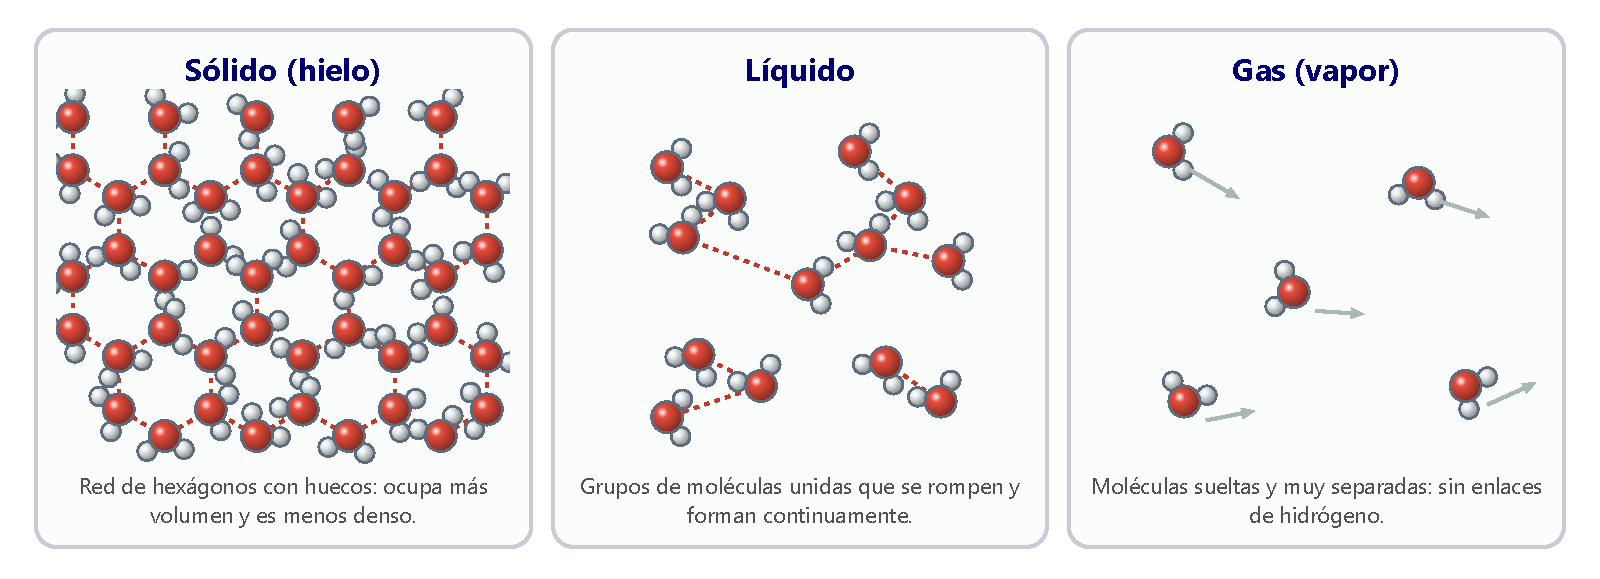
\includegraphics[width=\textwidth]{images/UD3/agua_estados}
    \caption{Enlaces de hidrógeno en el agua sólida, líquida y gaseosa.}
    \label{fig:agua_estados}
\end{figure}

\begin{exercise}
    Escribe el diagrama de Lewis del agua y explica cómo se forman los enlaces covalentes entre el oxígeno y los hidrógenos.
    \begin{solu}
        \chemfig{H-\charge{90=\:,270=\:}{O}-H}. El oxígeno tiene 6 electrones de valencia (\conf{2s^2~2p^4}) y le faltan dos; cada hidrógeno tiene uno y le falta otro. El oxígeno comparte \textcolor{red}{un par de electrones con cada hidrógeno}: se forman \textcolor{red}{dos enlaces covalentes sencillos} \ch{O-H}, y al oxígeno le quedan dos pares sin compartir.
    \end{solu}
\end{exercise}

\begin{exercise}
    ¿Por qué el agua tiene puntos de fusión y ebullición tan distintos de los del \ch{H2S}, el \ch{H2Se} y el \ch{H2Te}?
    \begin{solu}
        Porque entre las moléculas de agua hay \textcolor{red}{enlaces de hidrógeno} (el oxígeno es pequeño y atrae mucho a los electrones), mientras que en los otros hidruros del grupo 16 no los hay. Separar las moléculas de agua cuesta mucha más energía.
    \end{solu}
\end{exercise}

\begin{exercise}
    Observa un cristal de hielo (figura~\ref{fig:agua_estados}).
    \begin{enumerate}[label=\alph*)]
        \item ¿Qué enlaces hay en el cristal?
        \item ¿Qué les ocurre a las moléculas cuando el hielo se funde?
        \item ¿Qué enlaces hay en el agua líquida?
        \item ¿Qué ocurre cuando, finalmente, el agua hierve?
    \end{enumerate}
    \begin{solu}
        a) \textcolor{red}{Enlaces covalentes} \ch{O-H} dentro de cada molécula y \textcolor{red}{enlaces de hidrógeno} entre un H de una molécula y el O de otra. b) Se rompe parte de los enlaces de hidrógeno: las moléculas pierden la estructura de hexágonos y empiezan a moverse unas sobre otras. c) Covalentes dentro de las moléculas y enlaces de hidrógeno que unen grupos de moléculas y se rompen y forman continuamente. d) Se rompen todos los enlaces de hidrógeno: las moléculas quedan \textcolor{red}{sueltas}.
    \end{solu}
\end{exercise}

\subsection{Las fuerzas de Van der Waals}

En una molécula \textbf{apolar} los electrones se mueven continuamente. Si en un instante se acumulan más en un lado que en otro, el centro de las cargas negativas deja de coincidir con el de las positivas y aparece un \textbf{dipolo instantáneo}. Ese dipolo puede deformar la nube de electrones de una molécula vecina y crear en ella un \textbf{dipolo inducido} (figura~\ref{fig:van_der_waals}).

\begin{definition}[Fuerzas de Van der Waals]
    Son fuerzas de atracción electrostática entre \textbf{dipolos instantáneos o inducidos}. Son \textbf{más débiles} que los enlaces de hidrógeno y aparecen entre moléculas apolares (\ch{O2}, \ch{I2}, \ch{CH4}\ldots) e incluso entre átomos aislados (\ch{He}, \ch{Ne}\ldots). Son más intensas cuanto más grande es la molécula, porque tiene más electrones.
\end{definition}

\begin{figure}[H]
    \centering
    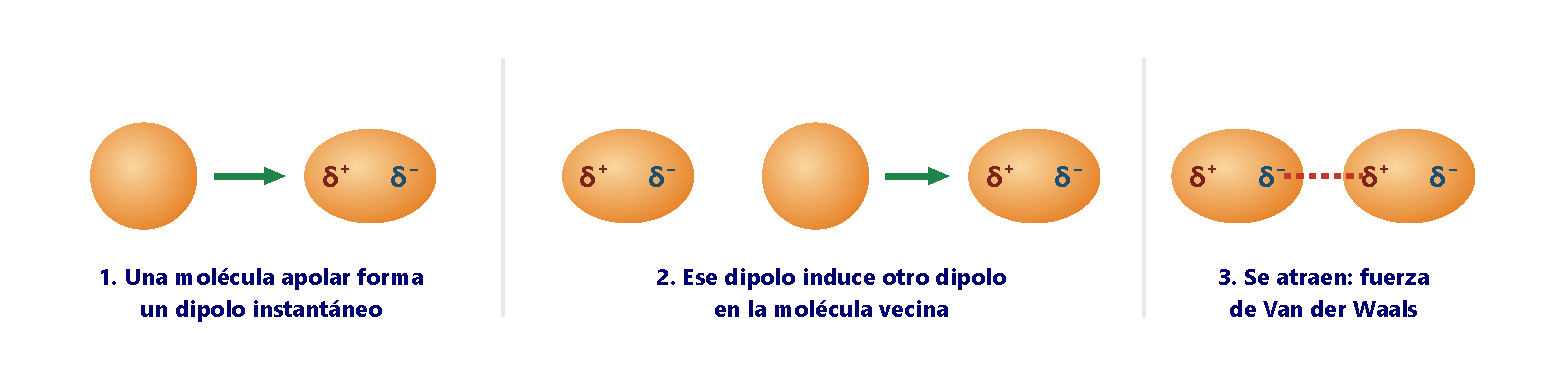
\includegraphics[width=\textwidth]{images/UD3/van_der_waals}
    \caption{Formación de un dipolo instantáneo, de un dipolo inducido y de la fuerza de Van der Waals entre ellos.}
    \label{fig:van_der_waals}
\end{figure}

\begin{remark}
    \textbf{El yodo, un cristal molecular.} El yodo forma cristales de color negro violáceo. Sus puntos de fusión y ebullición son mucho más altos que los del resto de los halógenos, lo que indica que sus moléculas no están aisladas: las moléculas \ch{I2} (dos átomos unidos por un enlace covalente sencillo) se mantienen unidas en una red por \textbf{fuerzas de Van der Waals}. Como estas fuerzas son débiles, el cristal se deshace con facilidad: el yodo \textbf{sublima} a temperatura ambiente. No conduce la electricidad porque no tiene electrones libres.
\end{remark}

\begin{exercise}
    ¿En qué se diferencian un dipolo permanente, uno instantáneo y uno inducido? Dibuja cómo se forma un dipolo instantáneo y cómo induce otro dipolo.
    \begin{solu}
        Un \textcolor{red}{dipolo permanente} (\ch{HCl}, \ch{H2O}\ldots) tiene siempre sus polos. Un \textcolor{red}{dipolo instantáneo} aparece solo durante un instante en una molécula apolar, por el movimiento de sus electrones. Un \textcolor{red}{dipolo inducido} se forma en una molécula apolar por la cercanía de otro dipolo (instantáneo o permanente). Dibujo como el de la figura~\ref{fig:van_der_waals}.
    \end{solu}
\end{exercise}

\begin{exercise}
    Explica las diferencias entre los puntos de fusión y ebullición de los halógenos:
    \begin{center}
        % --- tabla antigua ---
        % \begin{tblr}{colspec={lcc}, hlines, vlines, row{1}={bg=ocre!85, fg=white, font=\bfseries}, column{1}={bg=ocre!15}, cell{1}{1}={bg=ocre!85, fg=white}}
            % Halógeno & \(T_\text{f}\) (\unit{\celsius}) & \(T_\text{e}\) (\unit{\celsius}) \\
            % \ch{F2} & \num{-219.6} & \num{-188.2} \\
            % \ch{Cl2} & \num{-101.0} & \num{-34.7} \\
            % \ch{Br2} & \num{-7.2} & \num{58.8} \\
            % \ch{I2} & \num{113.7} & \num{184.3} \\
        % \end{tblr}
        % --- tabla nueva ---
        \begin{tabular}{@{}lcc@{}}
            \toprule
            \textbf{Halógeno} & \textbf{\(T_\text{f}\) (\unit{\celsius})} & \textbf{\(T_\text{e}\) (\unit{\celsius})} \\
            \midrule
            \ch{F2} & \num{-219.6} & \num{-188.2} \\[3pt]
            \ch{Cl2} & \num{-101.0} & \num{-34.7} \\[3pt]
            \ch{Br2} & \num{-7.2} & \num{58.8} \\[3pt]
            \ch{I2} & \num{113.7} & \num{184.3} \\
            \bottomrule
        \end{tabular}
    \end{center}
    \begin{solu}
        Todos están formados por moléculas apolares unidas por fuerzas de Van der Waals, que son \textcolor{red}{más intensas cuanto más grande es la molécula} (más electrones). Por eso las temperaturas aumentan del flúor al yodo: el flúor y el cloro son gases, el bromo es líquido y el yodo es un \textcolor{red}{sólido} cuyas moléculas forman un cristal molecular.
    \end{solu}
\end{exercise}

\begin{exercise}
    ¿Por qué no conducen la electricidad el yodo ni el diamante, y en cambio el grafito sí?
    \begin{solu}
        En el yodo y en el diamante todos los electrones están fijos en los enlaces: \textcolor{red}{no hay electrones libres}. En el grafito, cada carbono solo forma tres enlaces fuertes y su cuarto electrón \textcolor{red}{puede moverse} a lo largo de las capas.
    \end{solu}
\end{exercise}

\begin{exercise}
    Un elemento del grupo 17 forma, a temperatura ambiente, un sólido en el que las moléculas diatómicas están ordenadas en una red.
    \begin{enumerate}[label=\alph*)]
        \item ¿Puede tratarse del flúor, del cloro o del bromo? Justifícalo.
        \item ¿De qué elemento se trata?
        \item ¿Conduce la corriente eléctrica?
    \end{enumerate}
    \begin{solu}
        a) \textcolor{red}{No}: el flúor y el cloro son gases a temperatura ambiente y el bromo es líquido. b) Del \textcolor{red}{yodo}. c) \textcolor{red}{No}: no tiene electrones libres.
    \end{solu}
\end{exercise}

%========================================================================================
\section{Los compuestos iónicos}
%========================================================================================

Los átomos de muchos \textbf{metales} completan su último nivel \textbf{perdiendo electrones}, mientras que los de muchos \textbf{no metales} lo hacen \textbf{ganándolos}. Cuando se encuentran, el metal cede electrones al no metal: se forman \textbf{cationes} y \textbf{aniones}, que se atraen por tener cargas opuestas.

\subsection{¿Cómo se forma un compuesto iónico? El enlace iónico}

Veamos cómo se forma el cloruro de sodio, la sal común (figura~\ref{fig:formacion_nacl}):

\begin{enumerate}[label=\numberballblue]
    \item \textbf{Formación del ion sodio.} El sodio (\conf{[Ne]~3s^1}) tiene un solo electrón en su último nivel. Al perderlo, se queda con el nivel anterior completo: se forma el catión \ch{Na+}, con 11 protones y 10 electrones.
    \item \textbf{Formación del ion cloruro.} El cloro (\conf{[Ne]~3s^2~3p^5}) tiene siete electrones en su último nivel; al ganar uno lo completa y se convierte en el anión \ch{Cl-}, con 17 protones y 18 electrones.
    \item \textbf{Unión de los iones.} El \ch{Na+} y el \ch{Cl-} tienen cargas opuestas y se atraen por \textbf{fuerzas electrostáticas}: se ha formado un \textbf{enlace iónico}.
    \item \textbf{Formación del cristal.} Cada ion no se une a uno solo, sino que se rodea del mayor número posible de iones de signo contrario: se forma una \textbf{red cristalina iónica}. En el \ch{NaCl}, cada ion está rodeado por \textbf{seis} de signo contrario (figura~\ref{fig:cristal_nacl}).
\end{enumerate}

\begin{figure}[H]
    \centering
    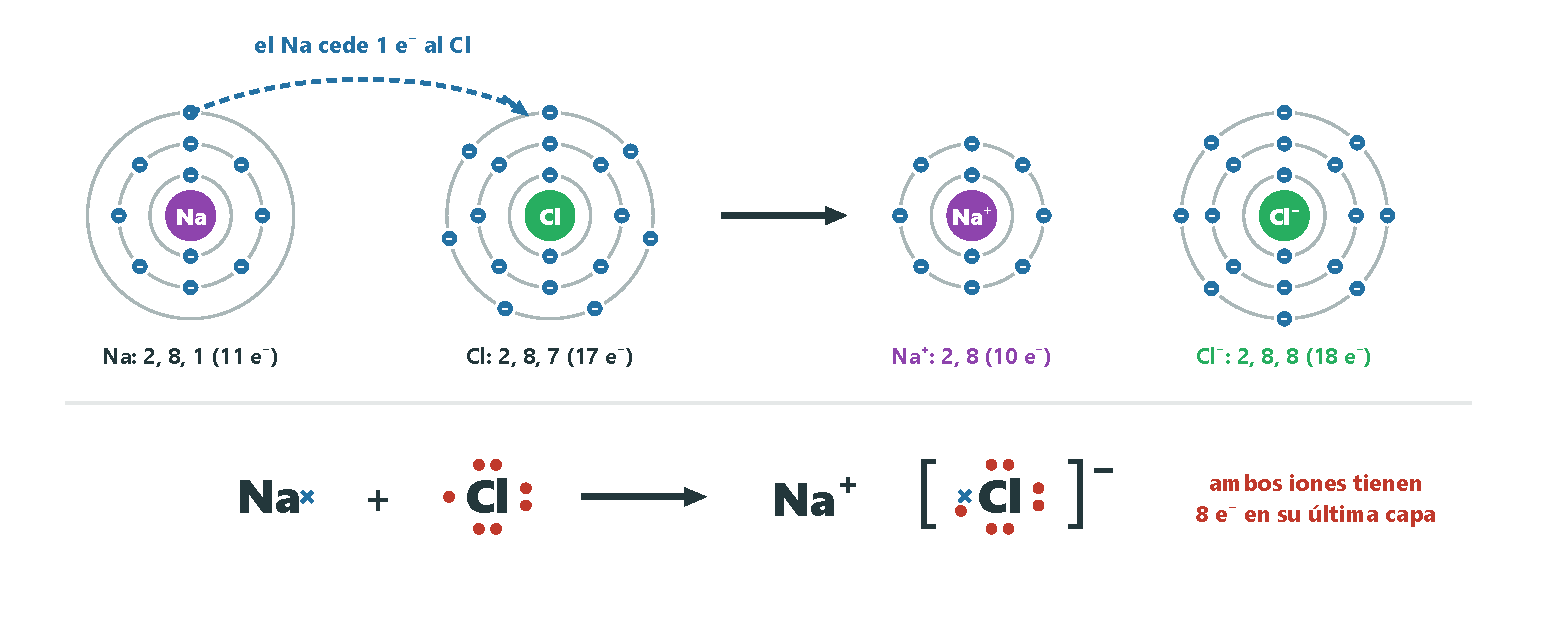
\includegraphics[width=\textwidth]{images/UD3/formacion_nacl}
    \caption{El sodio cede un electrón al cloro: ambos iones consiguen ocho electrones en su último nivel.}
    \label{fig:formacion_nacl}
\end{figure}

\begin{figure}[H]
    \centering
    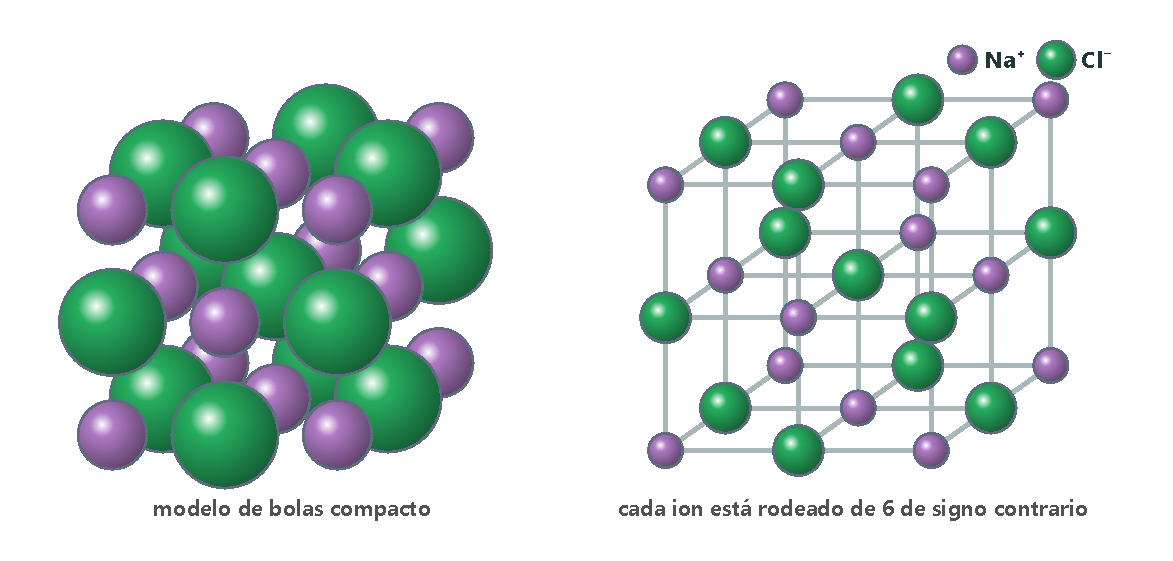
\includegraphics[width=0.75\textwidth]{images/UD3/cristal_nacl}
    \caption{Cristal de cloruro de sodio: modelo de bolas compacto y red cristalina.}
    \label{fig:cristal_nacl}
\end{figure}

\begin{definition}[Enlace iónico]
    Es la unión entre iones de signo contrario mediante fuerzas de atracción electrostática. Se da entre \textbf{metales} (que forman cationes) y \textbf{no metales} (que forman aniones). Los compuestos iónicos son \textbf{cristales}, no moléculas.
\end{definition}

La fórmula de un compuesto iónico solo indica la \textbf{proporción} entre los iones: es una \textbf{fórmula empírica}. \ch{NaCl} significa que hay un ion sodio por cada ion cloruro, y \ch{CaCl2}, que hay dos iones cloruro por cada ion calcio.

\begin{exercise}
    Observa la red de la figura~\ref{fig:cristal_nacl}. ¿Cuántos iones cloruro rodean a cada ion sodio? ¿Y cuántos iones sodio rodean a cada cloruro? ¿En qué proporción están ambos iones?
    \begin{solu}
        Cada \ch{Na+} está rodeado de \textcolor{red}{6} iones \ch{Cl-}, y cada \ch{Cl-}, de \textcolor{red}{6} iones \ch{Na+}. La proporción es \textcolor{red}{1:1}, como indica la fórmula \ch{NaCl}.
    \end{solu}
\end{exercise}

\begin{exercise}
    Explica, paso a paso y con diagramas de Lewis, cómo se forma el fluoruro de litio, \ch{LiF} (\(Z(\ch{Li}) = 3\), \(Z(\ch{F}) = 9\)).
    \begin{solu}
        \textcolor{blue}{1.} El litio (\conf{1s^2~2s^1}) pierde su electrón de valencia y forma \ch{Li+} (configuración del helio). \textcolor{blue}{2.} El flúor (\conf{1s^2~2s^2~2p^5}) gana ese electrón y forma \ch{F-} (configuración del neón). \textcolor{blue}{3.} Los iones se atraen electrostáticamente. \textcolor{blue}{4.} Cada ion se rodea de iones de signo contrario y se forma un cristal iónico.
        \[ \chemfig{\charge{90=\.}{Li}} \;+\; \chemfig{\charge{90=\:,0=\:,270=\:,180=\.}{F}} \;\longrightarrow\; \ch{Li+}\ \text{\ionlewis{\chemfig{\charge{90=\:,0=\:,270=\:,180=\:}{F}}}{-}} \]
    \end{solu}
\end{exercise}

\subsection{¿Qué propiedades tienen los compuestos iónicos?}

El enlace iónico se forma entre metales y no metales. Además del \ch{NaCl}, son compuestos iónicos el fluoruro de litio (\ch{LiF}), el bromuro de potasio (\ch{KBr}), el yoduro de potasio (\ch{KI}), el nitrato de calcio (\ch{Ca(NO3)2}) o el sulfato de bario (\ch{BaSO4}).

\begin{center}
    % --- tabla antigua ---
    % \begin{tblr}{colspec={llcc}, hlines, vlines, row{1}={bg=ocre!85, fg=white, font=\bfseries}, column{1-2}={bg=ocre!15}, cell{1}{1}={c=2}{bg=ocre!85, fg=white}, cell{2}{1}={c=2}{l}, cell{3}{1}={c=2}{l}, cell{4}{1}={c=2}{l}, cell{5}{1}={r=2}{l}, cell{7}{1}={c=2}{l}}
        % Propiedad & & Cloruro de sodio, \ch{NaCl} & Nitrato de calcio, \ch{Ca(NO3)2} \\
        % Aspecto & & cristales incoloros & cristales blancos \\
        % \(T_\text{f}\) (\unit{\celsius}) & & \num{801} & \num{561} \\
        % \(T_\text{e}\) (\unit{\celsius}) & & \num{1465} & se descompone antes \\
        % Conductividad & sólido & muy baja & muy baja \\
        % & fundido & alta & alta \\
        % Solubilidad en agua & & muy alta & alta \\
    % \end{tblr}
    % --- tabla nueva ---
    \begin{tabular}{@{}llcc@{}}
        \toprule
        \multicolumn{2}{c}{\textbf{Propiedad}} & \textbf{Cloruro de sodio, \ch{NaCl}} & \textbf{Nitrato de calcio, \ch{Ca(NO3)2}} \\
        \midrule
        \multicolumn{2}{c}{Aspecto} & cristales incoloros & cristales blancos \\[3pt]
        \multicolumn{2}{c}{\(T_\text{f}\) (\unit{\celsius})} & \num{801} & \num{561} \\[3pt]
        \multicolumn{2}{c}{\(T_\text{e}\) (\unit{\celsius})} & \num{1465} & se descompone antes \\[3pt]
        \multirow{2}{*}{Conductividad} & sólido & muy baja & muy baja \\[3pt]
         & fundido & alta & alta \\[3pt]
        \multicolumn{2}{c}{Solubilidad en agua} & muy alta & alta \\
        \bottomrule
    \end{tabular}
\end{center}

\begin{center}
    % --- tabla antigua ---
    % \begin{tblr}{colspec={X[3,l]X[5,l]}, hlines, vlines, row{1}={bg=ocre!85, fg=white, font=\bfseries, halign=c}}
        % Propiedad & Justificación \\
        % Son \textbf{sólidos cristalinos} a temperatura ambiente. & La atracción entre iones es muy intensa y se extiende en todas las direcciones: cada ion queda rodeado de iones de carga opuesta formando una red. \\
        % Tienen puntos de fusión y ebullición \textbf{elevados}. & Para que los iones abandonen sus posiciones en la red hay que vencer fuerzas muy intensas, lo que requiere mucha energía. \\
        % Son \textbf{duros}. & Para rayarlos hay que romper las fuertes uniones entre los iones. \\
        % Son \textbf{frágiles}. & Al golpearlos, una capa de iones se desplaza y quedan enfrentados iones del mismo signo, que se repelen: el cristal se rompe (figura~\ref{fig:golpe_ionico_metal}). \\
        % Muchos son \textbf{solubles en agua}. & Los dipolos del agua rodean a los iones y los separan de la red; se orientan de forma distinta según rodeen a un catión o a un anión (figura~\ref{fig:disolucion_ionico}). \\
        % \textbf{No conducen} la electricidad en estado sólido. & Los electrones están fijos en los iones y los iones no pueden moverse dentro del cristal. \\
        % \textbf{Conducen} la electricidad fundidos o disueltos. & Al fundirse o disolverse, los iones quedan libres y pueden transportar la corriente. \\
    % \end{tblr}
    % --- tabla nueva ---
    \begin{tabular}{@{}L{0.34\linewidth} L{0.57\linewidth}@{}}
        \toprule
        \textbf{Propiedad} & \textbf{Justificación} \\
        \midrule
        Son \textbf{sólidos cristalinos} a temperatura ambiente. & La atracción entre iones es muy intensa y se extiende en todas las direcciones: cada ion queda rodeado de iones de carga opuesta formando una red. \\[3pt]
        Tienen puntos de fusión y ebullición \textbf{elevados}. & Para que los iones abandonen sus posiciones en la red hay que vencer fuerzas muy intensas, lo que requiere mucha energía. \\[3pt]
        Son \textbf{duros}. & Para rayarlos hay que romper las fuertes uniones entre los iones. \\[3pt]
        Son \textbf{frágiles}. & Al golpearlos, una capa de iones se desplaza y quedan enfrentados iones del mismo signo, que se repelen: el cristal se rompe (figura~\ref{fig:golpe_ionico_metal}). \\[3pt]
        Muchos son \textbf{solubles en agua}. & Los dipolos del agua rodean a los iones y los separan de la red; se orientan de forma distinta según rodeen a un catión o a un anión (figura~\ref{fig:disolucion_ionico}). \\[3pt]
        \textbf{No conducen} la electricidad en estado sólido. & Los electrones están fijos en los iones y los iones no pueden moverse dentro del cristal. \\[3pt]
        \textbf{Conducen} la electricidad fundidos o disueltos. & Al fundirse o disolverse, los iones quedan libres y pueden transportar la corriente. \\
        \bottomrule
    \end{tabular}
\end{center}

\begin{figure}[H]
    \centering
    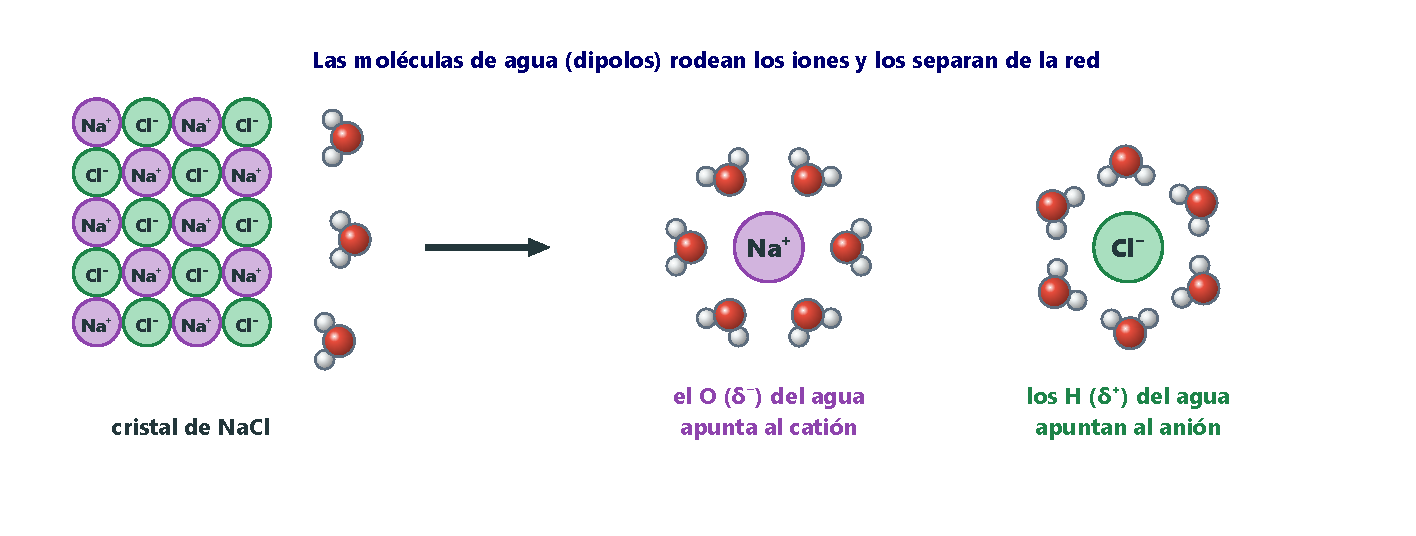
\includegraphics[width=0.85\textwidth]{images/UD3/disolucion_ionico}
    \caption{Disolución de un compuesto iónico en agua.}
    \label{fig:disolucion_ionico}
\end{figure}

\begin{exercise}
    Explica por qué el hecho de que la molécula de agua sea un dipolo facilita la disolución de los compuestos iónicos. Haz un dibujo del proceso.
    \begin{solu}
        Las moléculas de agua, que son dipolos, \textcolor{red}{rodean a los iones} del cristal y los separan de la red: orientan su extremo negativo (el oxígeno) hacia los cationes y su extremo positivo (los hidrógenos) hacia los aniones. Dibujo como el de la figura~\ref{fig:disolucion_ionico}.
    \end{solu}
\end{exercise}

\begin{exercise}
    Tienes dos frascos sin etiqueta con dos sólidos cristalinos de aspecto muy parecido. Uno es un compuesto iónico y el otro un compuesto covalente reticular. Si solo dispones de agua, ¿qué prueba harías para distinguirlos?
    \begin{solu}
        Intentaría disolver un poco de cada uno en agua: el que se disuelva será el \textcolor{red}{compuesto iónico} y el que no, el \textcolor{red}{covalente reticular}. (Además, la disolución del iónico conduciría la electricidad.)
    \end{solu}
\end{exercise}

\begin{exercise}
    Clasifica estos compuestos en iónicos o covalentes: \ch{CO2}, \ch{NaF}, \ch{H2S}, \ch{SiO2}, \ch{CaO}, \ch{NH3}, \ch{KBr}, \ch{HCl}.
    \begin{solu}
        \textcolor{blue}{Metal + no metal \(\to\) iónico; no metal + no metal \(\to\) covalente.} Iónicos: \textcolor{red}{\ch{NaF}, \ch{CaO}, \ch{KBr}}. Covalentes: \textcolor{red}{\ch{CO2}, \ch{H2S}, \ch{SiO2}, \ch{NH3}, \ch{HCl}}.
    \end{solu}
\end{exercise}

\begin{exercise}
    Indica si cada propiedad la presentan los compuestos covalentes cristalinos, los iónicos o ambos:
    \begin{enumerate}[label=\alph*)]
        \item Son sólidos cristalinos.
        \item Son muy duros.
        \item Tienen puntos de fusión y ebullición elevados.
        \item No conducen la electricidad en estado sólido.
        \item Se disuelven en agua.
        \item No se disuelven en agua.
        \item Conducen la electricidad fundidos o disueltos.
        \item Están formados por cationes y aniones.
    \end{enumerate}
    \begin{solu}
        a), b), c) y d): \textcolor{red}{ambos}. e) \textcolor{red}{Iónicos}. f) \textcolor{red}{Covalentes}. g) \textcolor{red}{Iónicos}. h) \textcolor{red}{Iónicos}.
    \end{solu}
\end{exercise}

\begin{exercise}
    La tabla recoge algunas propiedades de cuatro sustancias:
    \begin{center}
        % --- tabla antigua ---
        % \begin{tblr}{colspec={ccccc}, hlines, vlines, row{1-2}={bg=ocre!85, fg=white, font=\bfseries}, cell{1}{1}={r=2}{}, cell{1}{2}={r=2}{}, cell{1}{3}={c=2}{}, cell{1}{5}={r=2}{}}
            % Sustancia & \(T_\text{f}\) (\unit{\celsius}) & Conductividad & & ¿Soluble en agua? \\
            % & & sólido & disuelto & \\
            % A & \num{114} & no & no & no \\
            % B & \num{770} & no & sí & sí \\
            % C & \num{1710} & no & no & no \\
            % D & \num{690} & no & sí & sí \\
        % \end{tblr}
        % --- tabla nueva ---
        \begin{tabular}{@{}ccccc@{}}
            \toprule
            \multirow{2}{*}{\textbf{Sustancia}} & \multirow{2}{*}{\textbf{\(T_\text{f}\) (\unit{\celsius})}} & \multicolumn{2}{c}{\textbf{Conductividad}} & \multirow{2}{*}{\textbf{¿Soluble en agua?}} \\[3pt]
             &  & \textbf{sólido} & \textbf{disuelto} &  \\[3pt]
            A & \num{114} & no & no & no \\[3pt]
            B & \num{770} & no & sí & sí \\[3pt]
            C & \num{1710} & no & no & no \\[3pt]
            D & \num{690} & no & sí & sí \\
            \bottomrule
        \end{tabular}
    \end{center}
    \begin{enumerate}[label=\alph*)]
        \item ¿Cuáles son compuestos iónicos?
        \item ¿Cuál es un compuesto covalente molecular?
        \item ¿Cuál tiene un punto de fusión muy alto comparado con las demás? ¿Por qué no puede ser iónico?
    \end{enumerate}
    \begin{solu}
        a) \textcolor{red}{B y D}: se disuelven en agua y la disolución conduce. b) \textcolor{red}{A}: punto de fusión bajo, no conduce y no es soluble. c) \textcolor{red}{C}; no es iónico porque \textcolor{red}{no se disuelve} en agua: es un compuesto covalente reticular.
    \end{solu}
\end{exercise}

\begin{exercise}
    En un laboratorio se han obtenido cuatro sustancias sólidas, ninguna de las cuales conduce la electricidad en estado sólido:
    \begin{center}
        % --- tabla antigua ---
        % \begin{tblr}{colspec={X[c]X[c]X[c]X[c]}, hlines, vlines, row{1}={bg=ocre!85, fg=white, font=\bfseries}}
            % Sustancia A & Sustancia B & Sustancia C & Sustancia D \\
            % Formada por átomos de un solo elemento & Formada por dos elementos diferentes & Formada por dos elementos diferentes & Formada por dos elementos diferentes \\
            % Puntos de fusión y ebullición bajos & Puntos de fusión y ebullición elevados & Puntos de fusión y ebullición bajos & Puntos de fusión y ebullición elevados \\
            % Se disuelve en tetracloruro de carbono & No se disuelve en agua & No se disuelve en agua & Se disuelve en agua \\
        % \end{tblr}
        % --- tabla nueva ---
        \begin{tabular}{@{}C{0.21\linewidth} C{0.21\linewidth} C{0.21\linewidth} C{0.21\linewidth}@{}}
            \toprule
            \textbf{Sustancia A} & \textbf{Sustancia B} & \textbf{Sustancia C} & \textbf{Sustancia D} \\
            \midrule
            Formada por átomos de un solo elemento & Formada por dos elementos diferentes & Formada por dos elementos diferentes & Formada por dos elementos diferentes \\[3pt]
            Puntos de fusión y ebullición bajos & Puntos de fusión y ebullición elevados & Puntos de fusión y ebullición bajos & Puntos de fusión y ebullición elevados \\[3pt]
            Se disuelve en tetracloruro de carbono & No se disuelve en agua & No se disuelve en agua & Se disuelve en agua \\
            \bottomrule
        \end{tabular}
    \end{center}
    \begin{enumerate}[label=\alph*)]
        \item ¿Qué tipo de enlace propondrías para cada una?
        \item Si solo pudieras pedir \emph{una} prueba más para cada sustancia (conductividad fundida o disuelta, dureza, solubilidad en tetracloruro de carbono o fragilidad), ¿cuál elegirías para confirmar tu hipótesis?
    \end{enumerate}
    \begin{solu}
        a) A: \textcolor{red}{elemento que forma un cristal covalente molecular} (como el yodo). B: \textcolor{red}{compuesto covalente reticular}. C: \textcolor{red}{compuesto covalente molecular}. D: \textcolor{red}{compuesto iónico}.
        b) A: fragilidad (los cristales moleculares se deshacen con facilidad). B: dureza (los reticulares son muy duros). C: solubilidad en tetracloruro de carbono (los moleculares se disuelven en disolventes apolares). D: conductividad fundida o disuelta (los iónicos conducen en esos estados).
    \end{solu}
\end{exercise}

\begin{exercise}
    Explica, siguiendo los cuatro pasos de esta sección, cómo se forma un cristal de bromuro de potasio, \ch{KBr} (\(Z(\ch{K}) = 19\), \(Z(\ch{Br}) = 35\)).
    \begin{solu}
        \textcolor{blue}{1. Ion potasio:} el K (\conf{[Ar]~4s^1}) pierde su único electrón de valencia y forma \ch{K+}. \textcolor{blue}{2. Ion bromuro:} el Br (\conf{[Ar]~4s^2~3d^{10}~4p^5}) gana ese electrón y forma \ch{Br-}. \textcolor{blue}{3. Unión:} los iones de signo contrario se atraen por fuerzas electrostáticas (enlace iónico). \textcolor{blue}{4. Cristal:} cada ion se rodea del máximo número posible de iones de signo contrario y se forma una \textcolor{red}{red cristalina iónica} con proporción 1:1.
    \end{solu}
\end{exercise}

%========================================================================================
\section{El enlace metálico}
%========================================================================================

Los metales tienen propiedades muy diferentes de las del resto de los elementos porque sus átomos se unen mediante un enlace específico. Sus átomos suelen tener \textbf{uno, dos o tres electrones} en el último nivel, débilmente atraídos por el núcleo, por lo que pueden desplazarse o cederse con facilidad. El carácter metálico aumenta hacia la izquierda y hacia abajo en la tabla periódica.

Según la \textbf{teoría de los electrones libres}, cuando los átomos de un metal se aproximan todo lo posible, sus niveles exteriores se solapan y sus electrones de valencia dejan de pertenecer a un átomo concreto: se convierten en \textbf{electrones libres deslocalizados}.

\begin{definition}[Enlace metálico]
    Un \textbf{cristal metálico} está formado por \textbf{cationes} fijos y perfectamente ordenados, sumergidos en un «mar» o «gas» de \textbf{electrones libres} que se mueven por todo el cristal y mantienen unidos a los cationes.
\end{definition}

\begin{figure}[H]
    \centering
    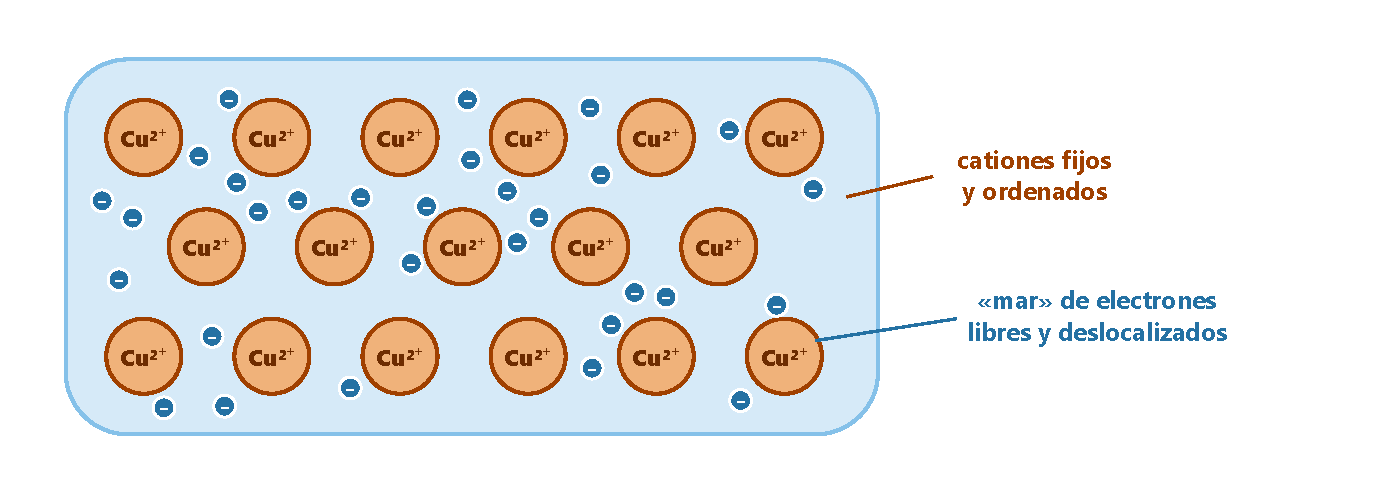
\includegraphics[width=0.8\textwidth]{images/UD3/enlace_metalico}
    \caption{Modelo del mar de electrones en un cristal de cobre.}
    \label{fig:enlace_metalico}
\end{figure}

Los átomos de los metales están muy \textbf{empaquetados}, por eso la densidad de los metales suele ser elevada. Los menos densos son los alcalinos (el litio flota en el agua) y el más denso es el osmio, con \qty{22.6}{\gram\per\cubic\centi\metre}.

\subsection{¿Cómo explica la teoría de los electrones libres las propiedades de los metales?}

\begin{itemize}
    \item \textbf{Duros, dúctiles y maleables.} Sus átomos están muy juntos, por lo que son difíciles de rayar. Sin embargo, una fuerza externa puede hacer que una capa de cationes se deslice sobre otra sin que el cristal se rompa, porque el mar de electrones sigue uniéndolos. Por eso los metales se pueden estirar en hilos (\textbf{ductilidad}) y extender en láminas (\textbf{maleabilidad}).
    \item \textbf{Buenos conductores de la electricidad.} Los electrones libres se mueven con facilidad hacia el polo positivo cuando se aplica una diferencia de potencial. La conductividad disminuye cuando el metal se funde.
    \item \textbf{Buenos conductores del calor.} Si se calienta una zona del metal, sus cationes vibran más y transmiten esa energía rápidamente a los vecinos (y también la transportan los electrones libres).
    \item \textbf{Puntos de fusión y ebullición elevados}, en general, porque hay que separar los átomos de una red muy compacta. Varían mucho: el mercurio es líquido a temperatura ambiente y el wolframio funde a \qty{3380}{\celsius}.
    \item \textbf{Brillo metálico}: reflejan casi toda la luz que reciben.
\end{itemize}

\begin{figure}[H]
    \centering
    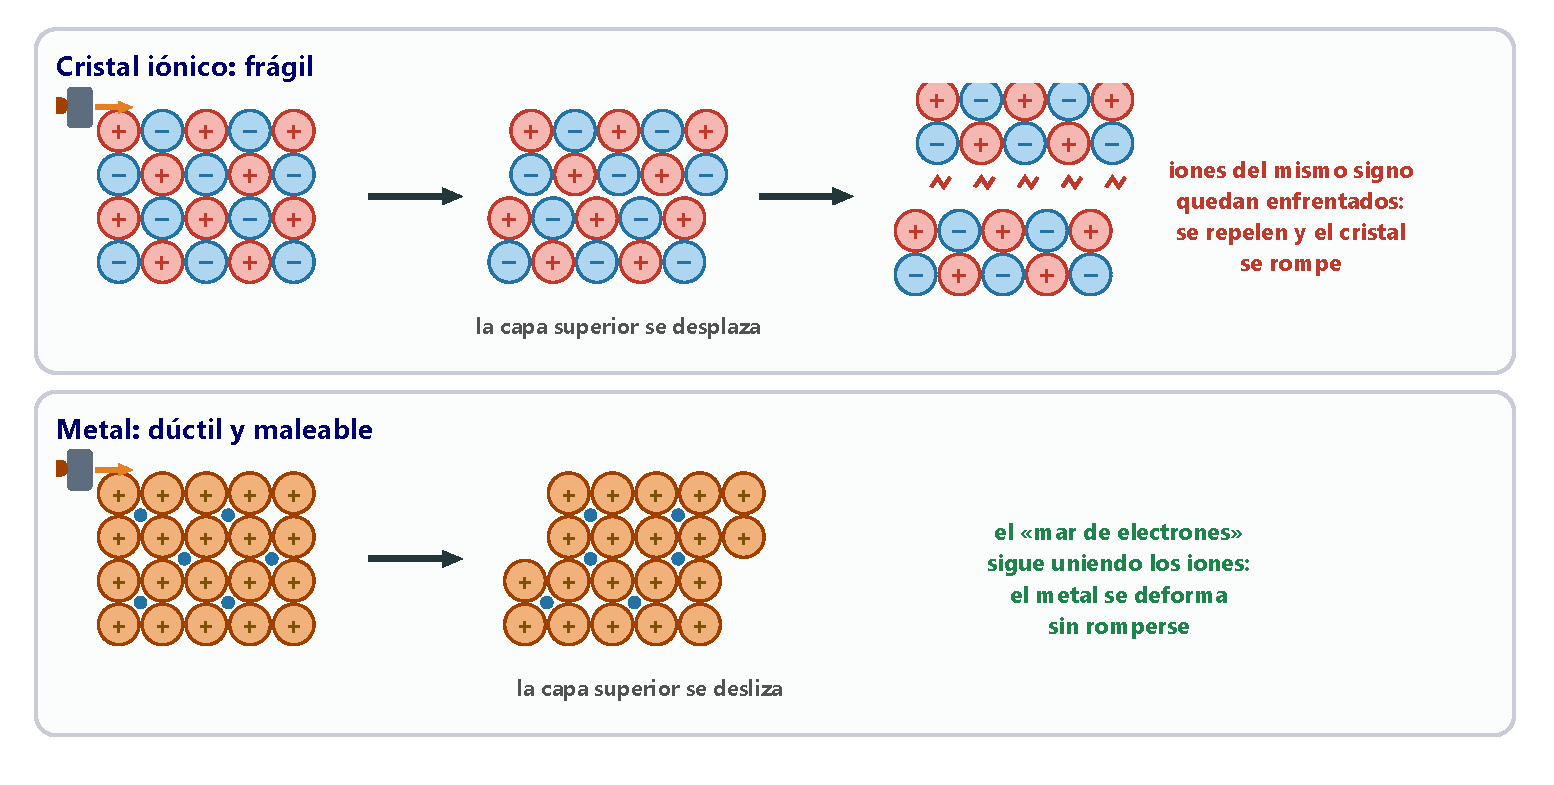
\includegraphics[width=\textwidth]{images/UD3/golpe_ionico_metal}
    \caption{Al golpear un cristal iónico, se enfrentan iones del mismo signo y se rompe; un metal se deforma sin romperse.}
    \label{fig:golpe_ionico_metal}
\end{figure}

\begin{example}
    \textbf{Ejercicio resuelto.} Estas dos gráficas muestran cómo varía la conductividad eléctrica de dos sólidos al calentarlos. ¿Cuál corresponde a un cristal iónico y cuál a uno metálico?

    \begin{center}
        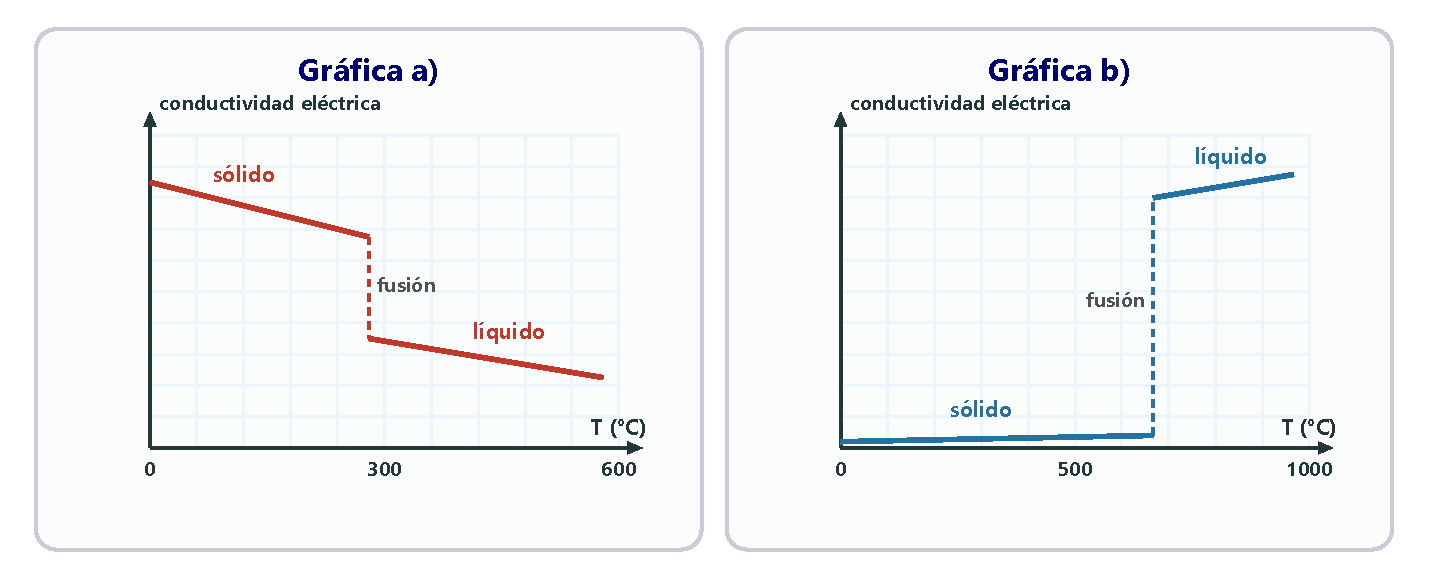
\includegraphics[width=0.8\textwidth]{images/UD3/conductividad_graficas}
    \end{center}

    \textcolor{blue}{Gráfica a):} la conductividad del sólido es muy alta, pero baja bruscamente al fundirse y es pequeña en el líquido. Es un \textcolor{red}{cristal metálico}: buen conductor en estado sólido, pero no tanto fundido.

    \textcolor{blue}{Gráfica b):} el sólido casi no conduce, pero la conductividad sube de golpe al fundirse. Es un \textcolor{red}{cristal iónico}: en el sólido no hay cargas que puedan moverse y, al fundirse, los iones quedan libres.
\end{example}

\begin{exercise}
    ¿Por qué los metales suelen tener densidades elevadas?
    \begin{solu}
        Porque sus átomos están muy \textcolor{red}{empaquetados}: en un volumen dado hay muchos átomos y, por tanto, mucha masa.
    \end{solu}
\end{exercise}

\begin{exercise}
    Busca la densidad de estos metales y ordénalos de menor a mayor: oro, potasio, aluminio, litio, plomo, sodio, hierro, platino.
    \begin{solu}
        \textcolor{blue}{Densidades aproximadas en \unit{\gram\per\cubic\centi\metre}:} Li \num{0.53}, K \num{0.86}, Na \num{0.97}, Al \num{2.70}, Fe \num{7.87}, Pb \num{11.3}, Au \num{19.3}, Pt \num{21.4}.
        \textcolor{red}{Li \(<\) K \(<\) Na \(<\) Al \(<\) Fe \(<\) Pb \(<\) Au \(<\) Pt}.
    \end{solu}
\end{exercise}

\begin{exercise}
    Explica con la teoría de los electrones libres por qué los metales conducen la electricidad.
    \begin{solu}
        Los electrones del enlace metálico están \textcolor{red}{libres y deslocalizados}: no pertenecen a ningún átomo y pueden moverse con gran facilidad por el cristal. Al aplicar una diferencia de potencial, se desplazan hacia el polo positivo: hay corriente eléctrica.
    \end{solu}
\end{exercise}

\begin{exercise}
    Compara lo que ocurre al golpear un sólido iónico y un metal. ¿Por qué el primero es frágil y el segundo dúctil y maleable?
    \begin{solu}
        En el sólido iónico, el golpe desplaza una capa de iones y quedan \textcolor{red}{enfrentados iones del mismo signo}, que se repelen: el cristal se rompe a lo largo de ese plano. En el metal, una capa de cationes se desliza sobre otra pero el \textcolor{red}{mar de electrones sigue uniéndolos}: el metal se deforma sin romperse (figura~\ref{fig:golpe_ionico_metal}).
    \end{solu}
\end{exercise}

\begin{exercise}
    Dadas las especies químicas \ch{Na+}, \ch{Br-}, \ch{He}, \ch{Cu}, \ch{N2}, \ch{CO2}, \ch{MgCl2}, elige:
    \begin{enumerate}[label=\alph*)]
        \item dos átomos;
        \item dos iones;
        \item dos elementos;
        \item dos moléculas;
        \item dos compuestos;
        \item un metal y un no metal.
    \end{enumerate}
    \begin{solu}
        a) \ch{He} y \ch{Cu}. b) \ch{Na+} y \ch{Br-}. c) Por ejemplo, \ch{Cu} y \ch{N2}. d) \ch{N2} y \ch{CO2}. e) \ch{CO2} y \ch{MgCl2}. f) \ch{Cu} (metal) y \ch{He} o \ch{N2} (no metales).
    \end{solu}
\end{exercise}

\begin{exercise}
    Indica qué afirmaciones son verdaderas y corrige las falsas:
    \begin{enumerate}[label=\alph*)]
        \item En el enlace metálico los electrones no pertenecen a ningún átomo concreto.
        \item Los metales se rayan con facilidad.
        \item Los metales funden a temperaturas bajas porque sus átomos se separan fácilmente.
        \item Los metales no conducen la electricidad porque no tienen electrones libres.
        \item Los metales tienen brillo.
        \item Los metales son buenos conductores del calor.
    \end{enumerate}
    \begin{solu}
        a) \textcolor{red}{Verdadera}. b) \textcolor{red}{Falsa}: sus átomos están muy juntos y son difíciles de rayar. c) \textcolor{red}{Falsa}: en general hace falta mucha energía para separar los átomos de la red, por lo que sus puntos de fusión son elevados. d) \textcolor{red}{Falsa}: gracias a sus electrones libres son muy buenos conductores. e) \textcolor{red}{Verdadera}. f) \textcolor{red}{Verdadera}.
    \end{solu}
\end{exercise}

\begin{exercise}
    Indica qué tipo de sustancia forma cada elemento (átomos aislados, moléculas covalentes, cristal covalente atómico, cristal covalente molecular o cristal metálico): \ch{Ne}, \ch{Al}, \ch{O2}, \ch{I2}, carbono (grafito), \ch{Ag}, carbono (diamante), \ch{Kr}, \ch{Pt}. ¿Cuáles conducen la electricidad?
    \begin{solu}
        Átomos aislados: \ch{Ne}, \ch{Kr}. Moléculas covalentes: \ch{O2}. Cristal covalente molecular: \ch{I2}. Cristales covalentes atómicos: grafito y diamante. Cristales metálicos: \ch{Al}, \ch{Ag}, \ch{Pt}.
        Conducen la electricidad: \textcolor{red}{\ch{Al}, \ch{Ag}, \ch{Pt} y el grafito}.
    \end{solu}
\end{exercise}

%========================================================================================
\section{Cantidad de sustancia. El mol y la masa molar}
%========================================================================================

En la tabla periódica aparece la masa atómica relativa de cada elemento. A partir de ellas podemos calcular la masa de las moléculas y de los compuestos.

\subsection{La masa molecular relativa}

\begin{definition}[Masa molecular relativa, \(M_r\)]
    La \textbf{masa molecular relativa} (o simplemente masa molecular) de un elemento o compuesto es la \textbf{suma de las masas atómicas relativas} de todos los átomos que aparecen en su fórmula. No tiene unidades.
\end{definition}

Se calcula igual sea cual sea la forma en que se presenta la sustancia:

\begin{center}
    % --- tabla antigua ---
    % \begin{tblr}{colspec={X[3,l]X[4,l]}, hlines, vlines, row{1}={bg=ocre!85, fg=white, font=\bfseries, halign=c}}
        % Tipo de sustancia & Ejemplo \\
        % Elemento formado por átomos aislados & \(M_r(\ch{Ne}) = A_r(\ch{Ne}) = \num{20.18}\) \\
        % Elemento formado por moléculas & \(M_r(\ch{O2}) = 2 \cdot 16 = 32\); \quad \(M_r(\ch{N2}) = 2 \cdot 14 = 28\) \\
        % Elemento en forma de cristal (covalente o metálico) & \(M_r(\ch{C}) = 12\); \quad \(M_r(\ch{Fe}) = 56\) \\
        % Compuesto iónico & \(M_r(\ch{NaCl}) = 23 + \num{35.5} = \num{58.5}\) (la fórmula solo indica la proporción de iones) \\
        % Compuesto covalente reticular & \(M_r(\ch{SiO2}) = 28 + 2 \cdot 16 = 60\) \\
        % Compuesto covalente molecular & \(M_r(\ch{H2O}) = 2 \cdot 1 + 16 = 18\); \quad \(M_r(\ch{HCl}) = 1 + \num{35.5} = \num{36.5}\) \\
    % \end{tblr}
    % --- tabla nueva ---
    \begin{tabular}{@{}L{0.39\linewidth} L{0.52\linewidth}@{}}
        \toprule
        \textbf{Tipo de sustancia} & \textbf{Ejemplo} \\
        \midrule
        Elemento formado por átomos aislados & \(M_r(\ch{Ne}) = A_r(\ch{Ne}) = \num{20.18}\) \\[3pt]
        Elemento formado por moléculas & \(M_r(\ch{O2}) = 2 \cdot 16 = 32\); \quad \(M_r(\ch{N2}) = 2 \cdot 14 = 28\) \\[3pt]
        Elemento en forma de cristal (covalente o metálico) & \(M_r(\ch{C}) = 12\); \quad \(M_r(\ch{Fe}) = 56\) \\[3pt]
        Compuesto iónico & \(M_r(\ch{NaCl}) = 23 + \num{35.5} = \num{58.5}\) (la fórmula solo indica la proporción de iones) \\[3pt]
        Compuesto covalente reticular & \(M_r(\ch{SiO2}) = 28 + 2 \cdot 16 = 60\) \\[3pt]
        Compuesto covalente molecular & \(M_r(\ch{H2O}) = 2 \cdot 1 + 16 = 18\); \quad \(M_r(\ch{HCl}) = 1 + \num{35.5} = \num{36.5}\) \\
        \bottomrule
    \end{tabular}
\end{center}

\begin{remark}
    \textbf{Masas atómicas que usaremos en esta sección:} H = 1; C = 12; N = 14; O = 16; F = 19; Na = 23; Mg = 24; Al = 27; Si = 28; S = 32; Cl = \num{35.5}; K = 39; Ca = 40; Fe = 56; Cu = \num{63.5}; Br = 80; Ag = 108; I = 127; Au = 197.
\end{remark}

\begin{exercise}
    Calcula la masa molecular relativa de:
    \begin{enumerate}[label=\alph*)]
        \item Dos elementos formados por átomos aislados: neón (\(A_r = \num{20.18}\)) y criptón (\(A_r = \num{83.80}\)).
        \item Tres elementos que forman cristales metálicos: potasio, plata y oro.
    \end{enumerate}
    \begin{solu}
        \textcolor{blue}{En los átomos aislados y en los cristales la masa molecular coincide con la masa atómica:}
        a) \(M_r(\ch{Ne}) = \textcolor{red}{\num{20.18}}\); \(M_r(\ch{Kr}) = \textcolor{red}{\num{83.80}}\). b) \(M_r(\ch{K}) = \textcolor{red}{39}\); \(M_r(\ch{Ag}) = \textcolor{red}{108}\); \(M_r(\ch{Au}) = \textcolor{red}{197}\).
    \end{solu}
\end{exercise}

\begin{exercise}
    Calcula la masa molecular relativa de estos elementos moleculares: oxígeno, \ch{O2}; cloro, \ch{Cl2}; yodo, \ch{I2}; nitrógeno, \ch{N2}.
    \begin{solu}
        \(M_r(\ch{O2}) = 2 \cdot 16 = \textcolor{red}{32}\); \(M_r(\ch{Cl2}) = 2 \cdot \num{35.5} = \textcolor{red}{71}\); \(M_r(\ch{I2}) = 2 \cdot 127 = \textcolor{red}{254}\); \(M_r(\ch{N2}) = 2 \cdot 14 = \textcolor{red}{28}\).
    \end{solu}
\end{exercise}

\begin{exercise}
    Calcula la masa molecular relativa de estos compuestos moleculares: dióxido de carbono, \ch{CO2}; sulfuro de hidrógeno, \ch{H2S}; trióxido de azufre, \ch{SO3}.
    \begin{solu}
        \(M_r(\ch{CO2}) = 12 + 2 \cdot 16 = \textcolor{red}{44}\); \(M_r(\ch{H2S}) = 2 \cdot 1 + 32 = \textcolor{red}{34}\); \(M_r(\ch{SO3}) = 32 + 3 \cdot 16 = \textcolor{red}{80}\).
    \end{solu}
\end{exercise}

\begin{exercise}
    Calcula la masa molecular relativa de estos compuestos cristalinos: cloruro de potasio, \ch{KCl}; trióxido de dialuminio, \ch{Al2O3}; tricloruro de hierro, \ch{FeCl3}.
    \begin{solu}
        \(M_r(\ch{KCl}) = 39 + \num{35.5} = \textcolor{red}{\num{74.5}}\); \(M_r(\ch{Al2O3}) = 2 \cdot 27 + 3 \cdot 16 = \textcolor{red}{102}\); \(M_r(\ch{FeCl3}) = 56 + 3 \cdot \num{35.5} = \textcolor{red}{\num{162.5}}\).
    \end{solu}
\end{exercise}

\subsection{La composición centesimal de un compuesto}

\begin{definition}[Composición centesimal]
    Es el \textbf{porcentaje en masa} de cada elemento en un compuesto. Como la fórmula de un compuesto es fija, su composición centesimal también lo es:
    \[ \%\,\text{elemento} = \frac{\text{n.º de átomos del elemento} \cdot A_r}{M_r} \cdot 100 \]
\end{definition}

\begin{example}
    \textbf{Composición centesimal del carbonato de sodio, \ch{Na2CO3}.}

    \textcolor{blue}{Masa molecular:} \(M_r = 2 \cdot 23 + 12 + 3 \cdot 16 = 106\).
    \[ \%\,\ch{Na} = \frac{46}{106} \cdot 100 = \textcolor{red}{\qty{43.4}{\percent}} \qquad \%\,\ch{C} = \frac{12}{106} \cdot 100 = \textcolor{red}{\qty{11.3}{\percent}} \qquad \%\,\ch{O} = \frac{48}{106} \cdot 100 = \textcolor{red}{\qty{45.3}{\percent}} \]
    La suma de los porcentajes siempre debe dar \num{100}.
\end{example}

\begin{example}
    \textbf{Composición centesimal del cloruro de magnesio, \ch{MgCl2}} (\(A_r(\ch{Mg}) = \num{24.3}\)).

    En el \ch{MgCl2} hay dos iones \ch{Cl-} por cada ion \ch{Mg^{2+}}: \(M_r = \num{24.3} + 2 \cdot \num{35.5} = \num{95.3}\).
    \[ \%\,\ch{Mg} = \frac{\num{24.3}}{\num{95.3}} \cdot 100 = \textcolor{red}{\qty{25.5}{\percent}} \qquad \%\,\ch{Cl} = \frac{71}{\num{95.3}} \cdot 100 = \textcolor{red}{\qty{74.5}{\percent}} \]
\end{example}

\begin{exercise}
    El cobre forma dos óxidos: el monóxido de cobre, \ch{CuO}, y el monóxido de dicobre, \ch{Cu2O}.
    \begin{enumerate}[label=\alph*)]
        \item Calcula la masa molecular relativa de cada uno.
        \item ¿Cuál tiene mayor porcentaje de cobre?
    \end{enumerate}
    \begin{solu}
        a) \(M_r(\ch{CuO}) = \num{63.5} + 16 = \textcolor{red}{\num{79.5}}\); \(M_r(\ch{Cu2O}) = 2 \cdot \num{63.5} + 16 = \textcolor{red}{143}\).
        b) \(\%\,\ch{Cu}(\ch{CuO}) = \frac{\num{63.5}}{\num{79.5}} \cdot 100 = \qty{79.9}{\percent}\); \(\%\,\ch{Cu}(\ch{Cu2O}) = \frac{127}{143} \cdot 100 = \qty{88.8}{\percent}\). Tiene más cobre el \textcolor{red}{\ch{Cu2O}}.
    \end{solu}
\end{exercise}

\begin{exercise}
    Copia y completa la tabla con los porcentajes de nitrógeno y de oxígeno de cada óxido.
    \begin{center}
        % --- tabla antigua ---
        % \begin{tblr}{colspec={lcc}, hlines, vlines, row{1}={bg=ocre!85, fg=white, font=\bfseries}, column{1}={bg=ocre!15}, cell{1}{1}={bg=ocre!85, fg=white}}
            % Sustancia & \% nitrógeno & \% oxígeno \\
            % \ch{N2O} & \ldots & \ldots \\
            % \ch{NO} & \ldots & \ldots \\
            % \ch{NO2} & \ldots & \ldots \\
            % \ch{N2O5} & \ldots & \ldots \\
        % \end{tblr}
        % --- tabla nueva ---
        \begin{tabular}{@{}lcc@{}}
            \toprule
            \textbf{Sustancia} & \textbf{\% nitrógeno} & \textbf{\% oxígeno} \\
            \midrule
            \ch{N2O} & \ldots & \ldots \\[3pt]
            \ch{NO} & \ldots & \ldots \\[3pt]
            \ch{NO2} & \ldots & \ldots \\[3pt]
            \ch{N2O5} & \ldots & \ldots \\
            \bottomrule
        \end{tabular}
    \end{center}
    \begin{solu}
        \textcolor{blue}{\(M_r\): \ch{N2O} = 44; \ch{NO} = 30; \ch{NO2} = 46; \ch{N2O5} = 108.}
        \begin{center}
            % --- tabla antigua ---
            % \begin{tblr}{colspec={lccc}, hlines, vlines, row{1}={font=\bfseries}}
                % Sustancia & \(M_r\) & \% N & \% O \\
                % \ch{N2O} & 44 & \(\frac{28}{44} \cdot 100 = \num{63.6}\) & \num{36.4} \\
                % \ch{NO} & 30 & \(\frac{14}{30} \cdot 100 = \num{46.7}\) & \num{53.3} \\
                % \ch{NO2} & 46 & \(\frac{14}{46} \cdot 100 = \num{30.4}\) & \num{69.6} \\
                % \ch{N2O5} & 108 & \(\frac{28}{108} \cdot 100 = \num{25.9}\) & \num{74.1} \\
            % \end{tblr}
            % --- tabla nueva ---
            \begin{tabular}{@{}lccc@{}}
                \toprule
                \textbf{Sustancia} & \textbf{\(M_r\)} & \textbf{\% N} & \textbf{\% O} \\
                \midrule
                \ch{N2O} & 44 & \(\frac{28}{44} \cdot 100 = \num{63.6}\) & \num{36.4} \\[3pt]
                \ch{NO} & 30 & \(\frac{14}{30} \cdot 100 = \num{46.7}\) & \num{53.3} \\[3pt]
                \ch{NO2} & 46 & \(\frac{14}{46} \cdot 100 = \num{30.4}\) & \num{69.6} \\[3pt]
                \ch{N2O5} & 108 & \(\frac{28}{108} \cdot 100 = \num{25.9}\) & \num{74.1} \\
                \bottomrule
            \end{tabular}
        \end{center}
    \end{solu}
\end{exercise}

\begin{exercise}
    ¿Cuál de estas sustancias tiene menor porcentaje de oxígeno?
    \begin{enumerate}[label=\alph*)]
        \item ozono, \ch{O3};
        \item hidróxido de potasio, \ch{KOH};
        \item dióxido de carbono, \ch{CO2};
        \item ácido nítrico, \ch{HNO3}.
    \end{enumerate}
    \begin{solu}
        a) \ch{O3}: \qty{100}{\percent}. b) \(M_r(\ch{KOH}) = 56\); \(\frac{16}{56} \cdot 100 = \qty{28.6}{\percent}\). c) \(M_r(\ch{CO2}) = 44\); \(\frac{32}{44} \cdot 100 = \qty{72.7}{\percent}\). d) \(M_r(\ch{HNO3}) = 63\); \(\frac{48}{63} \cdot 100 = \qty{76.2}{\percent}\).
        El menor porcentaje lo tiene el \textcolor{red}{\ch{KOH}, con un \qty{28.6}{\percent}}.
    \end{solu}
\end{exercise}

\begin{exercise}
    Calcula la masa molecular relativa del agua y su porcentaje de hidrógeno y de oxígeno.
    \begin{solu}
        \(M_r(\ch{H2O}) = 2 \cdot 1 + 16 = \textcolor{red}{18}\). \(\%\,\ch{H} = \frac{2}{18} \cdot 100 = \textcolor{red}{\qty{11.1}{\percent}}\); \(\%\,\ch{O} = \frac{16}{18} \cdot 100 = \textcolor{red}{\qty{88.9}{\percent}}\).
    \end{solu}
\end{exercise}

\begin{exercise}
    Calcula la masa molecular relativa del carbonato de magnesio, \ch{MgCO3}, y los porcentajes de magnesio, carbono y oxígeno.
    \begin{solu}
        \(M_r = 24 + 12 + 3 \cdot 16 = \textcolor{red}{84}\).
        \(\%\,\ch{Mg} = \frac{24}{84} \cdot 100 = \textcolor{red}{\qty{28.6}{\percent}}\); \(\%\,\ch{C} = \frac{12}{84} \cdot 100 = \textcolor{red}{\qty{14.3}{\percent}}\); \(\%\,\ch{O} = \frac{48}{84} \cdot 100 = \textcolor{red}{\qty{57.1}{\percent}}\).
    \end{solu}
\end{exercise}

\subsection{La cantidad de sustancia y el mol}

¿Qué tienen en común una docena de lápices, una de huevos y una de vasos? No tienen la misma masa ni ocupan el mismo volumen, pero en los tres casos hay \textbf{doce unidades}. En química pasa algo parecido: el número de átomos, moléculas o iones que intervienen en cualquier proceso es tan enorme que se ha definido una magnitud para contarlos «por paquetes».

\begin{definition}[Cantidad de sustancia y mol]
    La \textbf{cantidad de sustancia}, \(n\), es una magnitud fundamental del SI. Su unidad es el \textbf{mol}. Un mol contiene exactamente \(\num{6.02214076e23}\) entidades elementales (átomos, moléculas, iones, electrones\ldots). Este número fijo es la \textbf{constante de Avogadro}:
    \[ N_A = \qty{6.022e23}{\per\mol} \]
    Siempre hay que indicar de qué entidades se trata: no es lo mismo un mol de átomos de oxígeno que un mol de moléculas \ch{O2}.
\end{definition}

\begin{example}
    \textbf{De mol a partículas: \(N = n \cdot N_A\).} En \qty{0.01}{\mol} de \ch{I2} hay
    \[ N = \num{0.01} \cdot \num{6.022e23} = \textcolor{red}{\num{6.022e21}} \text{ moléculas de yodo} \]
    y, como cada molécula tiene dos átomos, \(2 \cdot \num{6.022e21} = \textcolor{red}{\num{1.2044e22}}\) átomos de yodo.

    \textbf{De partículas a mol: \(n = N / N_A\).} \num{6.022e24} átomos de plata equivalen a
    \[ n = \frac{\num{6.022e24}}{\qty{6.022e23}{\per\mol}} = \textcolor{red}{\qty{10}{\mol}} \text{ de átomos de plata} \]
\end{example}

\begin{exercise}
    ¿Cuántas partículas hay en\ldots
    \begin{enumerate}[label=\alph*)]
        \item \qty{2.0}{\mol} de moléculas?
        \item \qty{0.25}{\mol} de átomos?
        \item \qty{0.001}{\mol} de iones?
    \end{enumerate}
    \begin{solu}
        \textcolor{blue}{\(N = n \cdot N_A\):}
        a) \(2 \cdot \num{6.022e23} = \textcolor{red}{\num{1.2044e24}}\) moléculas. b) \(\num{0.25} \cdot \num{6.022e23} = \textcolor{red}{\num{1.5055e23}}\) átomos. c) \(\num{0.001} \cdot \num{6.022e23} = \textcolor{red}{\num{6.022e20}}\) iones.
    \end{solu}
\end{exercise}

\begin{exercise}
    ¿Qué cantidad de sustancia, en mol, hay en\ldots
    \begin{enumerate}[label=\alph*)]
        \item \num{3.011e23} átomos de hierro?
        \item \num{1.2044e22} moléculas de \ch{CO2}?
        \item \num{6.022e21} moléculas de agua?
    \end{enumerate}
    \begin{solu}
        \textcolor{blue}{\(n = N / N_A\):}
        a) \(\dfrac{\num{3.011e23}}{\num{6.022e23}} = \textcolor{red}{\qty{0.5}{\mol}}\). b) \(\dfrac{\num{1.2044e22}}{\num{6.022e23}} = \textcolor{red}{\qty{0.02}{\mol}}\). c) \(\dfrac{\num{6.022e21}}{\num{6.022e23}} = \textcolor{red}{\qty{0.01}{\mol}}\).
    \end{solu}
\end{exercise}

\begin{exercise}
    ¿Qué cantidad de sustancia hay en \num{1.5055e24} moléculas de oxígeno, \ch{O2}? ¿Cuántos átomos de oxígeno contienen?
    \begin{solu}
        \[ n = \frac{\num{1.5055e24}}{\qty{6.022e23}{\per\mol}} = \textcolor{red}{\qty{2.5}{\mol}} \text{ de } \ch{O2} \]
        Átomos: \(2 \cdot \num{1.5055e24} = \textcolor{red}{\num{3.011e24}}\) átomos de oxígeno.
    \end{solu}
\end{exercise}

\subsection{La masa molar}

\begin{definition}[Masa molar, \(M\)]
    La \textbf{masa molar} es la masa de \textbf{un mol} de átomos, moléculas, iones\ldots{} Se expresa en \unit{\kg\per\mol} o, más habitualmente, en \unit{\gram\per\mol}. Expresada en \unit{\gram\per\mol}, su valor numérico \textbf{coincide} con el de la masa atómica relativa o la masa molecular relativa.
\end{definition}

\begin{center}
    % --- tabla antigua ---
    % \begin{tblr}{colspec={X[l]X[l]}, hlines, vlines, row{1}={bg=ocre!85, fg=white, font=\bfseries, halign=c}}
        % A partir de la masa atómica relativa & A partir de la masa molecular relativa \\
        % \textbf{Átomos aislados:} \(A_r(\ch{Xe}) = \num{131.3}\) \(\Rightarrow\) \(M = \qty{131.3}{\gram\per\mol}\). & \textbf{Moléculas:} \(M_r(\ch{HCl}) = \num{36.5}\) \(\Rightarrow\) \(M = \qty{36.5}{\gram\per\mol}\). \\
        % \textbf{Cristales covalentes o metálicos:} \(A_r(\ch{C}) = 12\) \(\Rightarrow\) \(M = \qty{12}{\gram\per\mol}\); \(A_r(\ch{Au}) = 197\) \(\Rightarrow\) \(M = \qty{197}{\gram\per\mol}\). & \textbf{Cristales covalentes o iónicos:} \(M_r(\ch{SiO2}) = 60\) \(\Rightarrow\) \(M = \qty{60}{\gram\per\mol}\); \(M_r(\ch{NaCl}) = \num{58.5}\) \(\Rightarrow\) \(M = \qty{58.5}{\gram\per\mol}\). \\
    % \end{tblr}
    % --- tabla nueva ---
    \begin{tabular}{@{}L{0.45\linewidth} L{0.45\linewidth}@{}}
        \toprule
        \textbf{A partir de la masa atómica relativa} & \textbf{A partir de la masa molecular relativa} \\
        \midrule
        \textbf{Átomos aislados:} \(A_r(\ch{Xe}) = \num{131.3}\) \(\Rightarrow\) \(M = \qty{131.3}{\gram\per\mol}\). & \textbf{Moléculas:} \(M_r(\ch{HCl}) = \num{36.5}\) \(\Rightarrow\) \(M = \qty{36.5}{\gram\per\mol}\). \\[3pt]
        \textbf{Cristales covalentes o metálicos:} \(A_r(\ch{C}) = 12\) \(\Rightarrow\) \(M = \qty{12}{\gram\per\mol}\); \(A_r(\ch{Au}) = 197\) \(\Rightarrow\) \(M = \qty{197}{\gram\per\mol}\). & \textbf{Cristales covalentes o iónicos:} \(M_r(\ch{SiO2}) = 60\) \(\Rightarrow\) \(M = \qty{60}{\gram\per\mol}\); \(M_r(\ch{NaCl}) = \num{58.5}\) \(\Rightarrow\) \(M = \qty{58.5}{\gram\per\mol}\). \\
        \bottomrule
    \end{tabular}
\end{center}

\begin{exercise}
    Calcula la masa molar de:
    \begin{enumerate}[label=\alph*)]
        \item neón, \ch{Ne} (\(A_r = \num{20.18}\));
        \item hierro, \ch{Fe};
        \item oxígeno, \ch{O2};
        \item agua, \ch{H2O};
        \item cloruro de sodio, \ch{NaCl};
        \item carbonato de sodio, \ch{Na2CO3}.
    \end{enumerate}
    \begin{solu}
        a) \textcolor{red}{\qty{20.18}{\gram\per\mol}}. b) \textcolor{red}{\qty{56}{\gram\per\mol}}. c) \(2 \cdot 16 = \textcolor{red}{\qty{32}{\gram\per\mol}}\). d) \(2 + 16 = \textcolor{red}{\qty{18}{\gram\per\mol}}\). e) \(23 + \num{35.5} = \textcolor{red}{\qty{58.5}{\gram\per\mol}}\). f) \(46 + 12 + 48 = \textcolor{red}{\qty{106}{\gram\per\mol}}\).
    \end{solu}
\end{exercise}

\begin{exercise}
    Relaciona cada concepto con su definición.

    \textbf{Conceptos:} 1. Masa molecular relativa. 2. Mol. 3. Cantidad de sustancia. 4. Masa molar.

    \textbf{Definiciones:} a) Masa de un mol de partículas. b) Magnitud cuya unidad es el mol. c) Suma de las masas atómicas relativas de los átomos de una fórmula. d) Cantidad de sustancia que contiene \num{6.022e23} entidades.
    \begin{solu}
        \textcolor{red}{1--c; 2--d; 3--b; 4--a.}
    \end{solu}
\end{exercise}

\begin{exercise}
    ¿Cuál es la masa molar del bromo, \ch{Br2}?
    \begin{solu}
        \(M(\ch{Br2}) = 2 \cdot 80 = \textcolor{red}{\qty{160}{\gram\per\mol}}\).
    \end{solu}
\end{exercise}

\subsection{Relación entre masa, cantidad de sustancia y número de partículas}

La masa molar permite pasar de gramos a moles y al revés; la constante de Avogadro, de moles a número de partículas (figura~\ref{fig:mol_relaciones}):

\begin{centeredequation}
    n = \frac{m}{M} \qquad\qquad N = n \cdot N_A = \frac{m}{M} \cdot N_A
\end{centeredequation}

donde \(m\) es la masa en gramos, \(M\) la masa molar en \unit{\gram\per\mol}, \(n\) la cantidad de sustancia en mol y \(N\) el número de partículas.

\begin{figure}[H]
    \centering
    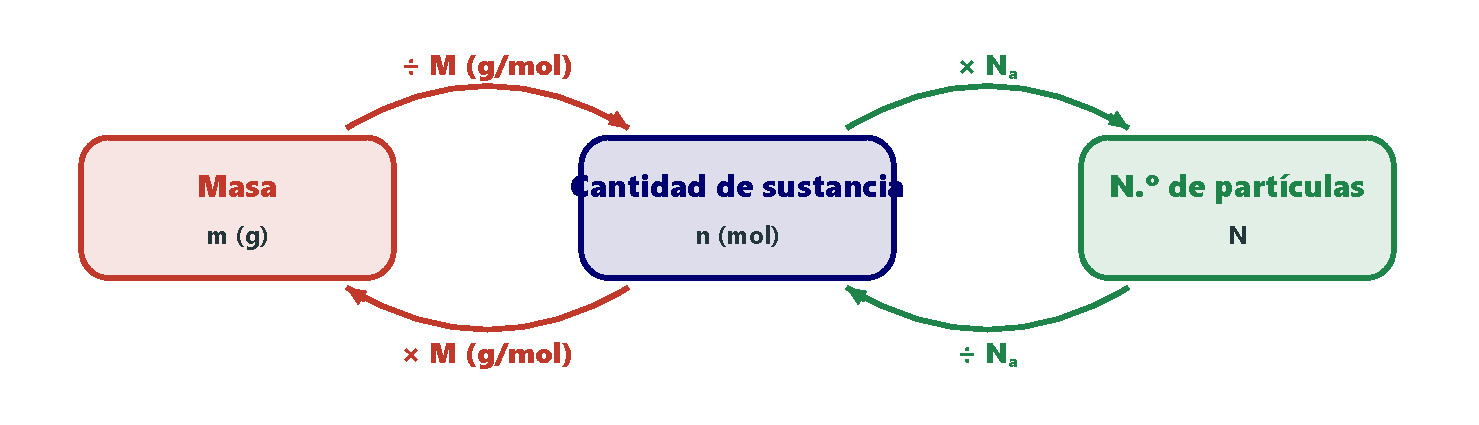
\includegraphics[width=0.85\textwidth]{images/UD3/mol_relaciones}
    \caption{Relación entre la masa, la cantidad de sustancia y el número de partículas.}
    \label{fig:mol_relaciones}
\end{figure}

\begin{example}
    \textbf{Algunos cálculos con el mol.}
    \begin{itemize}
        \item \textbf{¿Cuántos átomos hay en \qty{4}{\gram} de helio?} \(M(\ch{He}) = \qty{4}{\gram\per\mol}\); \(n = \frac{\qty{4}{\gram}}{\qty{4}{\gram\per\mol}} = \qty{1}{\mol}\); \(N = 1 \cdot \num{6.022e23} = \textcolor{red}{\num{6.022e23}}\) átomos.
        \item \textbf{¿Cuántas moléculas y átomos hay en \qty{2}{\mol} de cloro, \ch{Cl2}?} \(N = 2 \cdot \num{6.022e23} = \textcolor{red}{\num{1.2044e24}}\) moléculas, y el doble de átomos: \textcolor{red}{\num{2.4088e24}} átomos.
        \item \textbf{¿Qué masa tienen \num{1.2044e24} moléculas de agua?} \(n = \frac{\num{1.2044e24}}{\num{6.022e23}} = \qty{2}{\mol}\); \(m = n \cdot M = 2 \cdot 18 = \textcolor{red}{\qty{36}{\gram}}\).
        \item \textbf{¿Qué masa tienen \qty{1.5}{\mol} de \ch{HCl}?} \(m = \qty{1.5}{\mol} \cdot \qty{36.5}{\gram\per\mol} = \textcolor{red}{\qty{54.75}{\gram}}\).
        \item \textbf{¿Qué cantidad de sustancia hay en \qty{17}{\gram} de \ch{H2S}?} \(M = \qty{34}{\gram\per\mol}\); \(n = \frac{17}{34} = \textcolor{red}{\qty{0.5}{\mol}}\).
    \end{itemize}
\end{example}

\begin{exercise}
    Un frasco contiene \qty{63.5}{\gram} de yodo, \ch{I2}.
    \begin{enumerate}[label=\alph*)]
        \item ¿Qué cantidad de sustancia contiene?
        \item ¿Cuántas moléculas?
        \item ¿Cuántos átomos?
    \end{enumerate}
    \begin{solu}
        \textcolor{blue}{\(M(\ch{I2}) = 2 \cdot 127 = \qty{254}{\gram\per\mol}\).}
        a) \(n = \frac{\qty{63.5}{\gram}}{\qty{254}{\gram\per\mol}} = \textcolor{red}{\qty{0.25}{\mol}}\). b) \(N = \num{0.25} \cdot \num{6.022e23} = \textcolor{red}{\num{1.5055e23}}\) moléculas. c) \(2 \cdot \num{1.5055e23} = \textcolor{red}{\num{3.011e23}}\) átomos.
    \end{solu}
\end{exercise}

\begin{exercise}
    Un recipiente cerrado contiene \qty{16}{\gram} de dióxido de azufre, \ch{SO2}.
    \begin{enumerate}[label=\alph*)]
        \item ¿Cuál es la masa molar del \ch{SO2}?
        \item ¿Qué cantidad de sustancia contiene?
        \item ¿Cuántas moléculas hay?
        \item ¿Cuántos átomos de azufre y de oxígeno contiene?
    \end{enumerate}
    \begin{solu}
        a) \(M = 32 + 2 \cdot 16 = \textcolor{red}{\qty{64}{\gram\per\mol}}\). b) \(n = \frac{16}{64} = \textcolor{red}{\qty{0.25}{\mol}}\). c) \(N = \num{0.25} \cdot \num{6.022e23} = \textcolor{red}{\num{1.5055e23}}\) moléculas. d) Cada molécula tiene 1 átomo de S y 2 de O: \textcolor{red}{\num{1.5055e23}} átomos de S y \textcolor{red}{\num{3.011e23}} átomos de O.
    \end{solu}
\end{exercise}

\begin{exercise}
    Tienes \qty{8.8}{\gram} de \ch{CO2}.
    \begin{enumerate}[label=\alph*)]
        \item ¿Qué cantidad de sustancia hay en la muestra?
        \item ¿Cuántas moléculas contiene?
    \end{enumerate}
    \begin{solu}
        a) \(M(\ch{CO2}) = \qty{44}{\gram\per\mol}\); \(n = \frac{\num{8.8}}{44} = \textcolor{red}{\qty{0.2}{\mol}}\). b) \(N = \num{0.2} \cdot \num{6.022e23} = \textcolor{red}{\num{1.2044e23}}\) moléculas.
    \end{solu}
\end{exercise}

\begin{exercise}
    ¿Cuántos átomos hay en \qty{1}{\gram} de oro? ¿Cuál es la masa de un átomo de oro? ¿Y la de \num{3.011e24} átomos?
    \begin{solu}
        \textcolor{blue}{\(M(\ch{Au}) = \qty{197}{\gram\per\mol}\).}
        \(n = \frac{1}{197} = \qty{5.076e-3}{\mol}\); \(N = \num{5.076e-3} \cdot \num{6.022e23} = \textcolor{red}{\num{3.057e21}}\) átomos.
        Masa de un átomo: \(\dfrac{\qty{197}{\gram\per\mol}}{\qty{6.022e23}{\per\mol}} = \textcolor{red}{\qty{3.271e-22}{\gram}}\).
        \num{3.011e24} átomos son \(\frac{\num{3.011e24}}{\num{6.022e23}} = \qty{5}{\mol}\); \(m = 5 \cdot 197 = \textcolor{red}{\qty{985}{\gram}}\).
    \end{solu}
\end{exercise}

\begin{exercise}
    Calcula la masa de:
    \begin{enumerate}[label=\alph*)]
        \item \qty{0.25}{\mol} de átomos de cloro;
        \item \qty{0.25}{\mol} de moléculas de cloro, \ch{Cl2};
        \item \qty{2}{\mol} de átomos de oxígeno.
    \end{enumerate}
    \begin{solu}
        \textcolor{blue}{\(m = n \cdot M\):}
        a) \(\num{0.25} \cdot \num{35.5} = \textcolor{red}{\qty{8.875}{\gram}}\). b) \(\num{0.25} \cdot 71 = \textcolor{red}{\qty{17.75}{\gram}}\). c) \(2 \cdot 16 = \textcolor{red}{\qty{32}{\gram}}\) (que es la masa de \qty{1}{\mol} de moléculas \ch{O2}).
    \end{solu}
\end{exercise}

\begin{exercise}
    En una muestra de \qty{5.6}{\gram} de nitrógeno gaseoso, \ch{N2}, calcula:
    \begin{enumerate}[label=\alph*)]
        \item la cantidad de sustancia;
        \item el número de moléculas;
        \item el número de átomos.
    \end{enumerate}
    \begin{solu}
        a) \(n = \frac{\qty{5.6}{\gram}}{\qty{28}{\gram\per\mol}} = \textcolor{red}{\qty{0.2}{\mol}}\). b) \(N = \num{0.2} \cdot \num{6.022e23} = \textcolor{red}{\num{1.2044e23}}\) moléculas. c) \(2 \cdot \num{1.2044e23} = \textcolor{red}{\num{2.4088e23}}\) átomos.
    \end{solu}
\end{exercise}

\begin{exercise}
    ¿Cuál de estas muestras contiene más moléculas?
    \begin{enumerate}[label=\alph*)]
        \item \qty{10}{\gram} de agua, \ch{H2O};
        \item \qty{10}{\gram} de oxígeno, \ch{O2};
        \item \qty{10}{\gram} de hidrógeno, \ch{H2}.
    \end{enumerate}
    \begin{solu}
        \textcolor{blue}{Tendrá más moléculas la que tenga más moles:}
        a) \(n = \frac{10}{18} = \qty{0.56}{\mol}\). b) \(n = \frac{10}{32} = \qty{0.31}{\mol}\). c) \(n = \frac{10}{2} = \qty{5}{\mol}\). Tiene más moléculas el \textcolor{red}{hidrógeno}.
    \end{solu}
\end{exercise}

\begin{exercise}
    Calcula el número de moléculas que hay en:
    \begin{enumerate}[label=\alph*)]
        \item \qty{0.25}{\mol} de \ch{NH3};
        \item \qty{1.5}{\mol} de \ch{O2};
        \item \qty{36}{\gram} de agua;
        \item \qty{73}{\gram} de \ch{HCl}.
    \end{enumerate}
    \begin{solu}
        a) \(N = \num{0.25} \cdot \num{6.022e23} = \textcolor{red}{\num{1.5055e23}}\). b) \(N = \num{1.5} \cdot \num{6.022e23} = \textcolor{red}{\num{9.033e23}}\). c) \(n = \frac{36}{18} = \qty{2}{\mol}\); \(N = \textcolor{red}{\num{1.2044e24}}\). d) \(n = \frac{73}{\num{36.5}} = \qty{2}{\mol}\); \(N = \textcolor{red}{\num{1.2044e24}}\).
    \end{solu}
\end{exercise}

\begin{exercise}
    Calcula la masa de:
    \begin{enumerate}[label=\alph*)]
        \item \qty{0.5}{\mol} de \ch{HCl};
        \item \qty{2}{\mol} de \ch{CO2};
        \item \num{1.2044e22} moléculas de \ch{CH4};
        \item \num{1.5055e24} moléculas de \ch{NH3}.
    \end{enumerate}
    \begin{solu}
        a) \(m = \num{0.5} \cdot \num{36.5} = \textcolor{red}{\qty{18.25}{\gram}}\). b) \(m = 2 \cdot 44 = \textcolor{red}{\qty{88}{\gram}}\).
        c) \(n = \frac{\num{1.2044e22}}{\num{6.022e23}} = \qty{0.02}{\mol}\); \(m = \num{0.02} \cdot 16 = \textcolor{red}{\qty{0.32}{\gram}}\).
        d) \(n = \frac{\num{1.5055e24}}{\num{6.022e23}} = \qty{2.5}{\mol}\); \(m = \num{2.5} \cdot 17 = \textcolor{red}{\qty{42.5}{\gram}}\).
    \end{solu}
\end{exercise}


%------------------------------------------------


    \chapterimage{images/portada_cabeceras/cabecera_UD4}
    \chapter{La química del carbono}

    %! Author = crist
%! Date = 25/10/2026

\spacing{1.3}
%----------------------------------------------------------------------------------------
%	UNIDAD 4: LA QUÍMICA DEL CARBONO (4.º ESO)
%   Figuras: images/UD4/*.pdf (fuente HTML en images/UD4/html, SVG en images/UD4/svg).
%   Los modelos de bolas y varillas se generan con images/UD4/html/mol.js (geometría 3D real).
%   Fórmulas semidesarrolladas con \ch{...}: «-» enlace simple, «=» doble, «+» triple (CH+CH = etino).
%   Fórmulas desarrolladas y ramificadas con \chemfig{...}.
%   Masas atómicas: H = 1, C = 12, N = 14, O = 16, Cl = 35,5.
%----------------------------------------------------------------------------------------

% Mapa conceptual del tema (fuente en images/mapas_conceptuales/html/temas.js)
\begin{figure}[H]
    \centering
    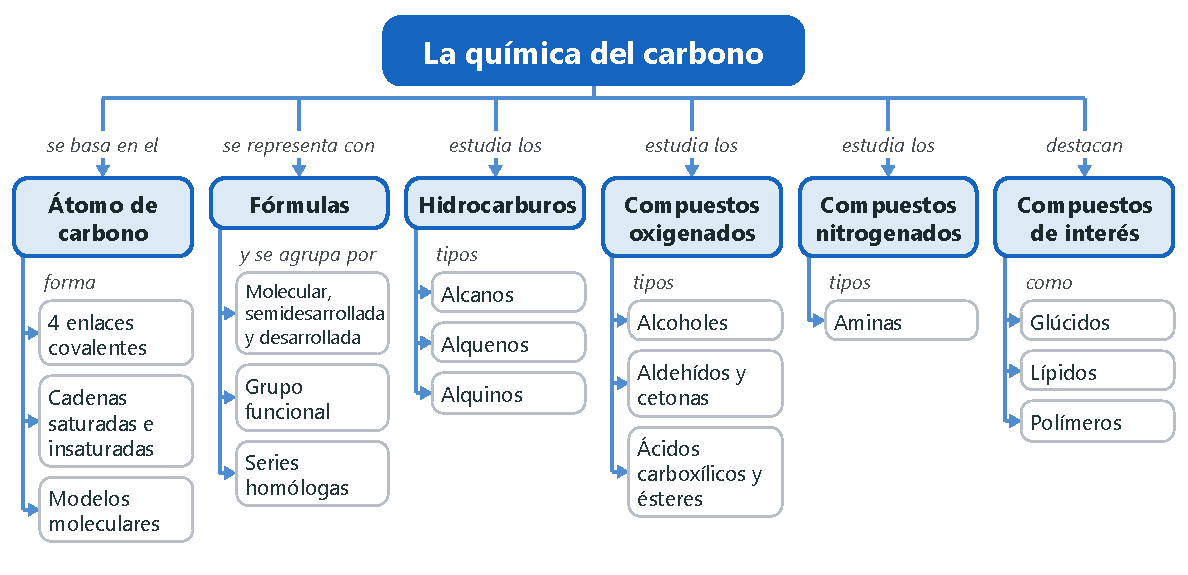
\includegraphics[width=\textwidth]{images/mapas_conceptuales/mapa_UD4}
\end{figure}

%========================================================================================
%\section*{Para empezar: la vida en la Tierra}
%\addcontentsline{toc}{section}{Para empezar: la vida en la Tierra}
%========================================================================================
%
%Las moléculas grandes se construyen con átomos que se «enganchan» con facilidad a otros átomos. El átomo de carbono, con cuatro electrones en su última capa, tiene esa cualidad: puede unirse a otros cuatro átomos, incluidos otros carbonos, y formar cadenas y anillos enormes. Por eso decimos que la vida en la Tierra está basada en el carbono.
%
%En las células hay cuatro tipos de moléculas esenciales, las \textbf{biomoléculas}:
%\begin{itemize}
%    \item Los \textbf{ácidos nucleicos} (ADN y ARN), que guardan y transmiten la información genética de generación en generación.
%    \item Las \textbf{proteínas}, formadas por cientos de moléculas más pequeñas, los \textbf{aminoácidos}. Cada aminoácido tiene un grupo amino (\ch{-NH2}) en un extremo y un grupo ácido (\ch{-COOH}) en el otro.
%    \item Los \textbf{hidratos de carbono} o \textbf{glúcidos}, que proporcionan el combustible a las células: glucosa, fructosa, sacarosa\ldots{} Muchas moléculas de glucosa enlazadas forman el almidón y la celulosa: la camiseta de algodón que llevas (celulosa) está hecha del mismo «ladrillo» que el azúcar que echas en el desayuno.
%    \item Los \textbf{lípidos}, moléculas orgánicas insolubles en agua, como las grasas y los aceites, que almacenan energía de forma muy eficiente.
%\end{itemize}
%
%Conocer la composición de la materia viva ayuda a garantizar una alimentación suficiente y sana (\textbf{ODS 2}, \emph{Hambre cero}) y a prevenir y tratar enfermedades, desarrollar vacunas y medicamentos (\textbf{ODS 3}, \emph{Salud y bienestar}). En esta unidad estudiaremos cómo es el átomo de carbono, cómo se unen los carbonos entre sí, cómo se nombran y formulan los compuestos del carbono más sencillos y qué propiedades y aplicaciones tienen.
%
%\begin{exercise}
%    ¿Por qué decimos que la vida en la Tierra está basada en el carbono?
%    \begin{solu}
%        Porque el carbono, con \textcolor{red}{cuatro electrones de valencia}, puede formar cuatro enlaces y unirse a otros átomos de carbono, dando lugar a las \textcolor{red}{cadenas y moléculas grandes} de las que están hechos los seres vivos (las biomoléculas).
%    \end{solu}
%\end{exercise}
%
%\begin{exercise}
%    ¿Qué moléculas transmiten la información genética? ¿De qué moléculas más pequeñas están formadas las proteínas y qué estructura tienen?
%    \begin{solu}
%        La información genética la transmiten los \textcolor{red}{ácidos nucleicos} (ADN y ARN). Las proteínas están formadas por \textcolor{red}{aminoácidos}, que tienen un \textcolor{red}{grupo amino}, \ch{-NH2}, y un \textcolor{red}{grupo ácido (carboxilo)}, \ch{-COOH}.
%    \end{solu}
%\end{exercise}
%
%\begin{exercise}
%    ¿Qué moléculas suministran el combustible a las células? ¿Por qué el texto compara el algodón con el azúcar?
%    \begin{solu}
%        Los \textcolor{red}{hidratos de carbono}, como la glucosa, la fructosa o la sacarosa. El algodón (celulosa) y el azúcar son \textcolor{red}{hidratos de carbono} y tienen el mismo «ladrillo» básico: la glucosa.
%    \end{solu}
%\end{exercise}
%
%\begin{exercise}
%    ¿Qué característica común tienen los lípidos y qué función cumplen? ¿Qué relación tienen las biomoléculas con los ODS 2 y 3?
%    \begin{solu}
%        Los lípidos son \textcolor{red}{insolubles en agua} y sirven para \textcolor{red}{almacenar energía}. Respuesta libre sobre los ODS: necesitamos ingerir a diario materia orgánica (glúcidos, lípidos, proteínas) para alimentarnos (ODS 2), y conocer las biomoléculas permite combatir la malnutrición y las enfermedades, y desarrollar vacunas y medicamentos (ODS 3).
%    \end{solu}
%\end{exercise}

%========================================================================================
\section{¿Qué características tiene el átomo de carbono?}
%========================================================================================

La vida en la Tierra se basa en la química del carbono, que tiene una gran facilidad para formar largas cadenas y anillos que pueden incluir otros elementos de la materia viva, como el hidrógeno, el oxígeno, el nitrógeno, el fósforo o el azufre. Se conocen más de diez millones de compuestos del carbono, muchos más que de todos los demás elementos juntos.

El carbono (\(Z = 6\)) está en el grupo 14 y el período 2 del sistema periódico. Su configuración electrónica es \conf{1s^2~2s^2~2p^2}: tiene \textbf{cuatro electrones de valencia} y le faltan otros cuatro para completar su capa de valencia. Por eso:
\begin{itemize}
    \item El carbono completa su capa uniéndose a otros átomos mediante \textbf{cuatro enlaces covalentes}, muy estables.
    \item Estos cuatro enlaces se dirigen en el espacio hacia los \textbf{vértices de un tetraedro regular}, con el átomo de carbono en el centro (figura~\ref{fig:tetraedro}).
\end{itemize}

\begin{figure}[H]
    \centering
    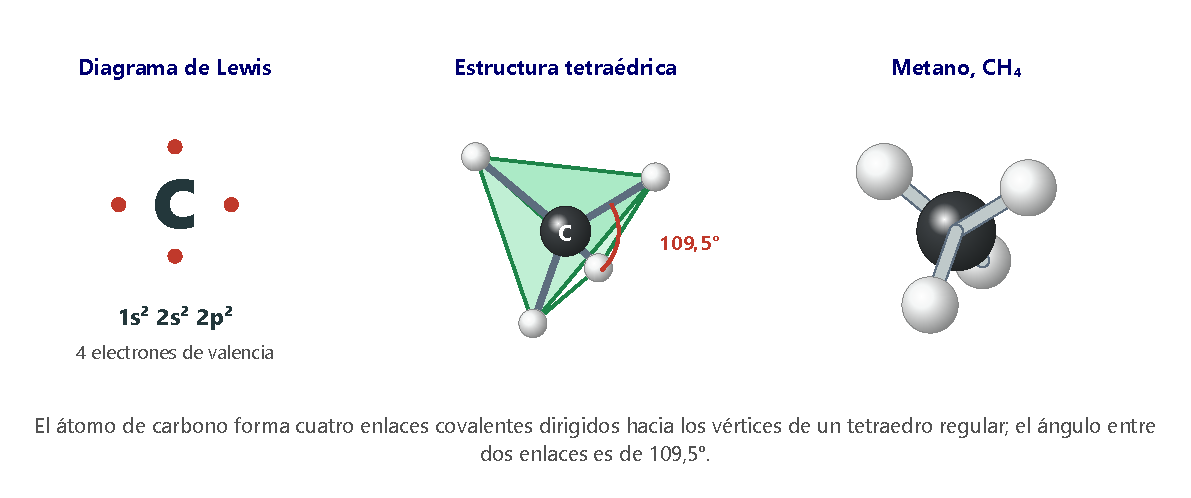
\includegraphics[width=0.95\textwidth]{images/UD4/tetraedro}
    \caption{Diagrama de Lewis y estructura tetraédrica del átomo de carbono.}
    \label{fig:tetraedro}
\end{figure}

\subsection{Los modelos moleculares en la química del carbono}

La estructura tetraédrica del carbono determina la forma de las moléculas de sus compuestos. Para ver cómo se orientan los átomos en el espacio usamos \textbf{modelos moleculares}, físicos o virtuales. Los más usados son los \textbf{modelos de bolas y varillas}: los átomos se representan con esferas y los enlaces con varillas, de modo que se aprecian los ángulos entre enlaces y si estos son simples, dobles o triples.

Por convenio, los átomos de carbono se dibujan de color gris o negro, los de hidrógeno de blanco, los de oxígeno de rojo, los de nitrógeno de azul y los de cloro o flúor de verde (figura~\ref{fig:modelos_moleculares}).

\begin{figure}[H]
    \centering
    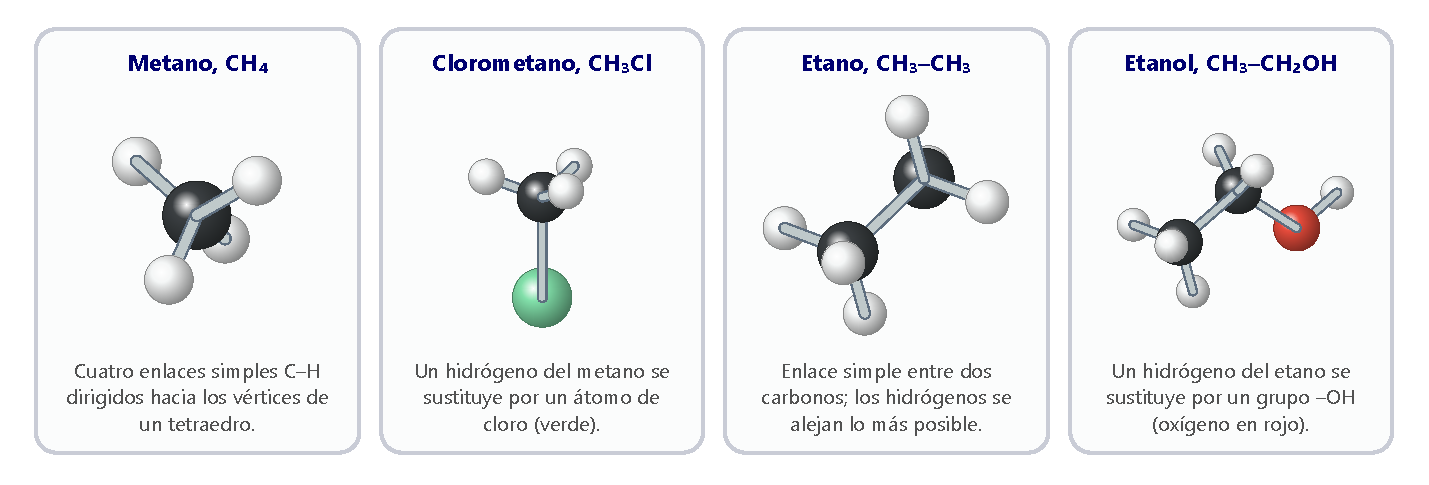
\includegraphics[width=\textwidth]{images/UD4/modelos_moleculares}
    \caption{Modelos de bolas y varillas de algunos compuestos del carbono.}
    \label{fig:modelos_moleculares}
\end{figure}

\begin{exercise}
    Observa el modelo de bolas y varillas del metano. ¿Es una molécula plana o tridimensional?
    \begin{solu}
        Es \textcolor{red}{tridimensional}: los cuatro hidrógenos están en los vértices de un tetraedro.
    \end{solu}
\end{exercise}

\subsection*{Actividades de consolidación: el átomo de carbono}

\begin{exercise}
    A comienzos del siglo \textsc{xix} se creía que los compuestos de los seres vivos solo podían formarse gracias a una «fuerza vital» que había en ellos, y por eso se llamaron \emph{compuestos orgánicos}. En 1828, Friedrich Wöhler sintetizó en su laboratorio la urea, un compuesto orgánico, sin ninguna fuerza vital. Desde entonces se habla de \emph{compuestos del carbono}.
    \begin{enumerate}[label=\alph*)]
        \item ¿Por qué hasta el siglo \textsc{xix} se distinguía entre compuestos orgánicos e inorgánicos?
        \item Según aquel criterio, clasifica: almidón, cloruro de sodio, glucosa, celulosa, agua, hemoglobina, arginina, triptófano, metano y etanol.
    \end{enumerate}
    \begin{solu}
        a) Porque se creía que los compuestos de los seres vivos solo se podían formar gracias a una \textcolor{red}{fuerza vital} presente en ellos.
        b) Orgánicos (los producen los seres vivos): \textcolor{red}{almidón, glucosa, celulosa, hemoglobina, arginina, triptófano, metano} (se forma al descomponerse la materia orgánica) y \textcolor{red}{etanol} (se forma en la fermentación). Inorgánicos: \textcolor{red}{cloruro de sodio y agua}.
    \end{solu}
\end{exercise}

\begin{exercise}
    Escribe la configuración electrónica del carbono y dibuja su diagrama de Lewis. a) ¿Cuántos electrones de valencia tiene? b) ¿Cuántos le faltan para completar el nivel 2? c) ¿Cuántos enlaces covalentes puede formar?
    \begin{solu}
        \conf{1s^2~2s^2~2p^2}; Lewis: \quad\chemfig{\charge{90=\.,0=\.,270=\.,180=\.}{C}}\quad.
        a) \textcolor{red}{Cuatro}. b) \textcolor{red}{Cuatro} (el nivel 2 se completa con ocho electrones). c) \textcolor{red}{Cuatro} enlaces covalentes.
    \end{solu}
\end{exercise}

\begin{exercise}
    En la figura~\ref{fig:modelos_moleculares}, identifica: a) dos compuestos con dos átomos de carbono; b) dos compuestos con un solo carbono; c) un compuesto con cloro; d) un compuesto con oxígeno.
    \begin{solu}
        a) El \textcolor{red}{etano} y el \textcolor{red}{etanol}. b) El \textcolor{red}{metano} y el \textcolor{red}{clorometano}. c) El \textcolor{red}{clorometano}. d) El \textcolor{red}{etanol}.
    \end{solu}
\end{exercise}

\begin{exercise}
    Sitúa el carbono en el sistema periódico: a) ¿en qué grupo y período está? b) ¿Cuál es su número atómico?
    \begin{solu}
        a) \textcolor{red}{Grupo 14, período 2}. b) \(Z = \textcolor{red}{6}\).
    \end{solu}
\end{exercise}

\begin{exercise}
    Dibuja la estructura tetraédrica del átomo de carbono. ¿Qué tipo de enlace lo une a los otros cuatro átomos?
    \begin{solu}
        El carbono ocupa el centro de un tetraedro y sus cuatro enlaces apuntan a los vértices, formando ángulos de \ang{109.5} (figura~\ref{fig:tetraedro}). Son \textcolor{red}{enlaces covalentes}.
    \end{solu}
\end{exercise}

\begin{exercise}
    Dibuja una cadena de dos átomos de carbono unidos y complétala con seis hidrógenos, uno en cada vértice libre de los tetraedros. ¿Qué compuesto es?
    \begin{solu}
        Es el \textcolor{red}{etano}, \ch{CH3-CH3}: cada carbono está unido al otro carbono y a tres hidrógenos (figura~\ref{fig:modelos_moleculares}).
    \end{solu}
\end{exercise}

%========================================================================================
\section{¿Cómo son los enlaces carbono-carbono?}
%========================================================================================

El átomo de carbono puede unirse mediante sus cuatro enlaces covalentes a átomos de otros elementos (hidrógeno, oxígeno, nitrógeno, halógenos\ldots), pero sobre todo a otros átomos de carbono, formando \textbf{cadenas carbonadas}, que son el esqueleto de los compuestos del carbono.

Dos átomos de carbono pueden unirse entre sí mediante un enlace simple, doble o triple, según compartan uno, dos o tres pares de electrones (figura~\ref{fig:enlaces_cc}):

\begin{center}
    % --- tabla antigua ---
    % \begin{tblr}{colspec={X[l]X[l]X[l]}, hlines, vlines, row{1}={bg=ocre!85, fg=white, font=\bfseries}, cells={font=\small}}
        % Enlace simple, C--C & Enlace doble, C=C & Enlace triple, C\(\equiv\)C \\
        % Comparten \textbf{un par} de electrones. & Comparten \textbf{dos pares} de electrones. & Comparten \textbf{tres pares} de electrones. \\
        % Estructura \textbf{tridimensional}. A cada carbono le quedan tres enlaces para unirse a otros átomos. & Los dos carbonos y los átomos unidos a ellos están en el \textbf{mismo plano}. A cada carbono le quedan dos enlaces. & Los dos carbonos y los átomos unidos a ellos están en \textbf{línea recta}. A cada carbono le queda un enlace. \\
        % Etano: \ch{CH3-CH3} & Eteno: \ch{CH2=CH2} & Etino: \ch{CH+CH} \\
    % \end{tblr}
    % --- tabla nueva ---
    {\small
    \begin{tabular}{@{}L{0.29\linewidth} L{0.29\linewidth} L{0.29\linewidth}@{}}
        \toprule
        \textbf{Enlace simple, C--C} & \textbf{Enlace doble, C=C} & \textbf{Enlace triple, C\(\equiv\)C} \\
        \midrule
        Comparten \textbf{un par} de electrones. & Comparten \textbf{dos pares} de electrones. & Comparten \textbf{tres pares} de electrones. \\[3pt]
        Estructura \textbf{tridimensional}. A cada carbono le quedan tres enlaces para unirse a otros átomos. & Los dos carbonos y los átomos unidos a ellos están en el \textbf{mismo plano}. A cada carbono le quedan dos enlaces. & Los dos carbonos y los átomos unidos a ellos están en \textbf{línea recta}. A cada carbono le queda un enlace. \\[3pt]
        Etano: \ch{CH3-CH3} & Eteno: \ch{CH2=CH2} & Etino: \ch{CH+CH} \\
        \bottomrule
    \end{tabular}
    }
\end{center}

\begin{figure}[H]
    \centering
    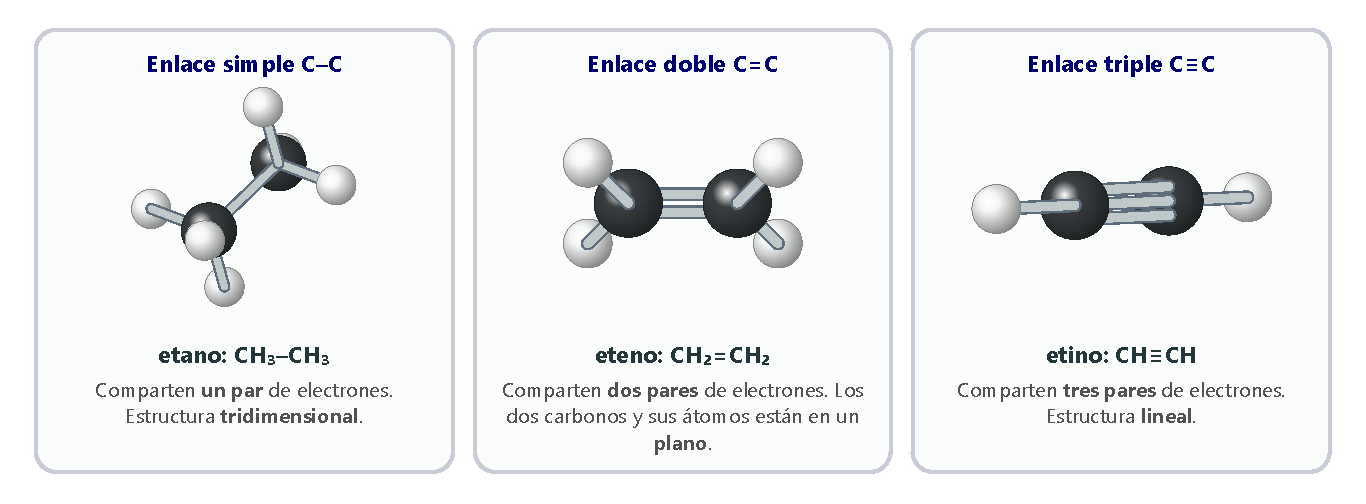
\includegraphics[width=\textwidth]{images/UD4/enlaces_cc}
    \caption{Modelos moleculares del etano, el eteno y el etino.}
    \label{fig:enlaces_cc}
\end{figure}

\subsection{¿Qué diferencia hay entre una cadena saturada y una insaturada?}

\begin{itemize}
    \item Una \textbf{cadena saturada} solo tiene enlaces carbono-carbono simples. Por ejemplo, el pentano: \ch{CH3-CH2-CH2-CH2-CH3}.
    \item Una \textbf{cadena insaturada} tiene, al menos, un enlace carbono-carbono doble o triple. Por ejemplo: \ch{CH3-CH=CH-CH2-CH3} y \ch{CH3-C+CH}.
\end{itemize}

\begin{exercise}
    ¿Cuántos electrones comparten dos átomos de carbono unidos por un doble enlace? ¿Y por un triple enlace?
    \begin{solu}
        Por un doble enlace, \textcolor{red}{cuatro} electrones (dos pares); por un triple enlace, \textcolor{red}{seis} electrones (tres pares).
    \end{solu}
\end{exercise}

\subsection*{Actividades de consolidación: los enlaces carbono-carbono}

\begin{exercise}
    Señala si es verdadero o falso y justifica tu respuesta:
    \begin{enumerate}[label=\alph*)]
        \item Si en una cadena hay dos carbonos unidos por un enlace doble o triple, la cadena no puede ser saturada.
        \item Dos carbonos que comparten dos pares de electrones están unidos por un enlace triple.
        \item Los enlaces entre los átomos de carbono son iónicos.
        \item Una molécula en la que todos los enlaces entre carbonos son simples es plana.
    \end{enumerate}
    \begin{solu}
        a) \textcolor{red}{Verdadero}: es insaturada. b) \textcolor{red}{Falso}: es un enlace doble. c) \textcolor{red}{Falso}: son covalentes. d) \textcolor{red}{Falso}: es tridimensional.
    \end{solu}
\end{exercise}

\begin{exercise}
    Escribe la fórmula de una cadena carbonada de cuatro carbonos que tenga: a) solo enlaces simples; b) al menos un doble enlace; c) al menos un triple enlace.
    \begin{solu}
        Respuesta abierta. Por ejemplo: a) \textcolor{red}{\ch{CH3-CH2-CH2-CH3}}; b) \textcolor{red}{\ch{CH2=CH-CH2-CH3}}; c) \textcolor{red}{\ch{CH+C-CH2-CH3}}.
    \end{solu}
\end{exercise}

\begin{exercise}
    Indica si cada enunciado corresponde al enlace simple, al doble o al triple:
    a) los carbonos comparten tres pares de electrones; b) se representa C=C; c) estructura tridimensional; d) se representa C--C; e) los carbonos y los átomos unidos a ellos están en un plano; f) estructura lineal; g) los carbonos comparten un par de electrones; h) los carbonos comparten dos pares de electrones.
    \begin{solu}
        Enlace simple: \textcolor{red}{c), d) y g)}. Enlace doble: \textcolor{red}{b), e) y h)}. Enlace triple: \textcolor{red}{a) y f)}.
    \end{solu}
\end{exercise}

\begin{exercise}
    En un modelo de bolas y varillas, ¿cómo distinguirías una molécula con un enlace C--C simple, otra con uno doble y otra con uno triple?
    \begin{solu}
        Por el número de varillas entre los dos carbonos (\textcolor{red}{una, dos o tres}) y por la forma: con enlace simple la molécula es \textcolor{red}{tridimensional}; con doble, los átomos unidos a los carbonos están en un \textcolor{red}{plano}; con triple, en \textcolor{red}{línea recta} (figura~\ref{fig:enlaces_cc}).
    \end{solu}
\end{exercise}

%========================================================================================
\section{¿Cómo son las fórmulas en la química del carbono?}
%========================================================================================

Una \textbf{fórmula química} es la expresión abreviada de la composición de una molécula. Para los compuestos del carbono usamos cuatro tipos de fórmulas. Por ejemplo, para el butano:

\begin{center}
    % --- tabla antigua ---
    % \begin{tblr}{colspec={Q[l,m,0.24\textwidth]X[l,m]}, hlines, vlines, column{1}={font=\bfseries\small}, cells={font=\small}}
        % Fórmula molecular & Indica cuántos átomos de cada elemento hay en la molécula, pero no cómo están unidos. Butano: \ch{C4H10}. \\
        % Fórmula semidesarrollada & Solo se escriben los enlaces entre carbonos (y con los grupos funcionales); los demás átomos se agrupan con el carbono al que están unidos. Butano: \ch{CH3-CH2-CH2-CH3}. \\
        % Fórmula desarrollada o estructural & Muestra todos los átomos y todos los enlaces, pero no su disposición en el espacio. Butano: \setchemfig{atom sep=1.7em}\chemfig{H-C(-[2]H)(-[6]H)-C(-[2]H)(-[6]H)-C(-[2]H)(-[6]H)-C(-[2]H)(-[6]H)-H} \\
        % Fórmula geométrica & Representa en el plano la molécula tridimensional: los enlaces que salen hacia el observador se dibujan con cuñas, y los que se alejan, con cuñas de trazo discontinuo. Es lo más parecido a un modelo de bolas y varillas. \\
    % \end{tblr}
    % --- tabla nueva ---
    {\small
    \begin{tabular}{@{}l L{0.78\linewidth}@{}}
        \toprule
        \textbf{Fórmula molecular} & Indica cuántos átomos de cada elemento hay en la molécula, pero no cómo están unidos. Butano: \ch{C4H10}. \\[3pt]
        \textbf{Fórmula semidesarrollada} & Solo se escriben los enlaces entre carbonos (y con los grupos funcionales); los demás átomos se agrupan con el carbono al que están unidos. Butano: \ch{CH3-CH2-CH2-CH3}. \\[3pt]
        \textbf{Fórmula desarrollada o estructural} & Muestra todos los átomos y todos los enlaces, pero no su disposición en el espacio. Butano: \setchemfig{atom sep=1.7em}\chemfig{H-C(-[2]H)(-[6]H)-C(-[2]H)(-[6]H)-C(-[2]H)(-[6]H)-C(-[2]H)(-[6]H)-H} \\[3pt]
        \textbf{Fórmula geométrica} & Representa en el plano la molécula tridimensional: los enlaces que salen hacia el observador se dibujan con cuñas, y los que se alejan, con cuñas de trazo discontinuo. Es lo más parecido a un modelo de bolas y varillas. \\
        \bottomrule
    \end{tabular}
    }
\end{center}

\begin{center}
    % --- tabla antigua ---
    % \begin{tblr}{colspec={Q[l,m]Q[c,m]Q[c,m]Q[c,m]Q[c,m]}, hlines, vlines, row{1}={bg=ocre!85, fg=white, font=\bfseries\small}, column{1}={font=\bfseries\small}, cell{1}{1}={bg=ocre!85, fg=white}, cells={font=\small}}
        % Molécula & Metano & Clorometano & Eteno & Etanal \\
        % Molecular & \ch{CH4} & \ch{CH3Cl} & \ch{C2H4} & \ch{C2H4O} \\
        % Semidesarrollada & \ch{CH4} & \ch{CH3Cl} & \ch{CH2=CH2} & \ch{CH3-CHO} \\
        % Desarrollada & \chemfig{C(-[0]H)(-[2]H)(-[4]H)(-[6]H)} & \chemfig{C(-[0]H)(-[2]H)(-[4]H)(-[6]Cl)} & \chemfig{C(-[3]H)(-[5]H)=C(-[1]H)(-[7]H)} & \chemfig{H-C(-[2]H)(-[6]H)-C(=[1]O)(-[7]H)} \\
    % \end{tblr}
    % --- tabla nueva ---
    {\small
    \begin{tabular}{@{}lcccc@{}}
        \toprule
        \textbf{Molécula} & \textbf{Metano} & \textbf{Clorometano} & \textbf{Eteno} & \textbf{Etanal} \\
        \midrule
        \textbf{Molecular} & \ch{CH4} & \ch{CH3Cl} & \ch{C2H4} & \ch{C2H4O} \\[3pt]
        \textbf{Semidesarrollada} & \ch{CH4} & \ch{CH3Cl} & \ch{CH2=CH2} & \ch{CH3-CHO} \\[3pt]
        \textbf{Desarrollada} & \chemfig{C(-[0]H)(-[2]H)(-[4]H)(-[6]H)} & \chemfig{C(-[0]H)(-[2]H)(-[4]H)(-[6]Cl)} & \chemfig{C(-[3]H)(-[5]H)=C(-[1]H)(-[7]H)} & \chemfig{H-C(-[2]H)(-[6]H)-C(=[1]O)(-[7]H)} \\
        \bottomrule
    \end{tabular}
    }
\end{center}

\subsection{¿Por qué ciertos compuestos del carbono tienen propiedades parecidas? Grupo funcional y serie homóloga}

\begin{definition}[Grupo funcional]
    Un \textbf{grupo funcional} es un átomo o conjunto de átomos responsable del comportamiento químico de la molécula. Por ejemplo, todos los alcoholes tienen el grupo \ch{-OH}, que les da propiedades parecidas.
\end{definition}

\begin{definition}[Serie homóloga]
    Una \textbf{serie homóloga} es un grupo de compuestos que tienen el mismo grupo funcional pero cadenas con distinto número de átomos de carbono. Sus propiedades físicas y químicas son semejantes.
\end{definition}

En las fórmulas generales, la letra \textbf{R} (o R\('\), R\(''\)) representa un \textbf{radical}: una cadena de carbonos a la que le falta un hidrógeno, que se ha sustituido por el grupo funcional. Por ejemplo, el eteno, el propeno y el but-1-eno (con el grupo C=C) son gases en condiciones normales y reaccionan con el agua para dar alcoholes.

\subsection{¿Cómo se nombran y formulan los compuestos del carbono?}

Para formular y nombrar los compuestos del carbono se siguen las reglas de la IUPAC:
\begin{enumerate}[label=\numberballblue]
    \item Se localiza la \textbf{cadena principal}: la cadena carbonada más larga (si hay grupo funcional, la más larga que lo contenga).
    \item Se \textbf{numeran} sus carbonos empezando por el extremo más próximo al grupo funcional o, si no lo hay, a un sustituyente, de modo que los números (\emph{localizadores}) sean lo más bajos posible.
    \item Se nombran los \textbf{sustituyentes} (radicales) delante del nombre de la cadena, cada uno precedido de su localizador y un guion. Si hay varios, se separan los números con comas y se ordenan alfabéticamente.
    \item Los dobles y triples enlaces y los grupos funcionales se localizan igual, con el número delante de la terminación del nombre.
    \item El nombre tiene un \textbf{prefijo}, que indica el número de carbonos de la cadena principal, y un \textbf{sufijo}, que indica el grupo funcional.
\end{enumerate}

\begin{center}
    % --- tabla antigua ---
    % \begin{tblr}{colspec={cccccccccc}, hlines, vlines, row{1}={bg=ocre!85, fg=white, font=\bfseries}, cells={font=\small}}
        % 1 & 2 & 3 & 4 & 5 & 6 & 7 & 8 & 9 & 10 \\
        % met- & et- & prop- & but- & pent- & hex- & hept- & oct- & non- & dec- \\
    % \end{tblr}
    % --- tabla nueva ---
    {\small
    \begin{tabular}{@{}cccccccccc@{}}
        \toprule
        \textbf{1} & \textbf{2} & \textbf{3} & \textbf{4} & \textbf{5} & \textbf{6} & \textbf{7} & \textbf{8} & \textbf{9} & \textbf{10} \\
        \midrule
        met- & et- & prop- & but- & pent- & hex- & hept- & oct- & non- & dec- \\
        \bottomrule
    \end{tabular}
    }
\end{center}

\begin{center}
    % --- tabla antigua ---
    % \begin{tblr}{colspec={lcccl}, hlines, vlines, row{1}={bg=ocre!85, fg=white, font=\bfseries}, cells={font=\small}}
        % Serie homóloga & Grupo funcional & Sufijo & Ejemplo & Nombre \\
        % Alcanos & C--C & -ano & \ch{CH3-CH3} & etano \\
        % Alquenos & C=C & -eno & \ch{CH2=CH2} & eteno \\
        % Alquinos & C\(\equiv\)C & -ino & \ch{CH+CH} & etino \\
        % Alcoholes & \ch{-OH} (hidroxilo) & -ol & \ch{CH3OH} & metanol \\
        % Aldehídos & \ch{-CHO} (carbonilo) & -al & \ch{H-CHO} & metanal \\
        % Cetonas & \ch{-CO\bond{single}} (carbonilo) & -ona & \ch{CH3-CO-CH3} & propanona \\
        % Ácidos carboxílicos & \ch{-COOH} (carboxilo) & -oico & \ch{CH3-COOH} & ácido etanoico \\
        % Ésteres & \ch{-COO\bond{single}} & -oato de -ilo & \ch{CH3-COO-CH3} & etanoato de metilo \\
        % Aminas & \ch{-NH2} (amino) & -amina & \ch{CH3-CH2-NH2} & etilamina \\
    % \end{tblr}
    % --- tabla nueva ---
    {\small
    \begin{tabular}{@{}lcccl@{}}
        \toprule
        \textbf{Serie homóloga} & \textbf{Grupo funcional} & \textbf{Sufijo} & \textbf{Ejemplo} & \textbf{Nombre} \\
        \midrule
        Alcanos & C--C & -ano & \ch{CH3-CH3} & etano \\[3pt]
        Alquenos & C=C & -eno & \ch{CH2=CH2} & eteno \\[3pt]
        Alquinos & C\(\equiv\)C & -ino & \ch{CH+CH} & etino \\[3pt]
        Alcoholes & \ch{-OH} (hidroxilo) & -ol & \ch{CH3OH} & metanol \\[3pt]
        Aldehídos & \ch{-CHO} (carbonilo) & -al & \ch{H-CHO} & metanal \\[3pt]
        Cetonas & \ch{-CO\bond{single}} (carbonilo) & -ona & \ch{CH3-CO-CH3} & propanona \\[3pt]
        Ácidos carboxílicos & \ch{-COOH} (carboxilo) & -oico & \ch{CH3-COOH} & ácido etanoico \\[3pt]
        Ésteres & \ch{-COO\bond{single}} & -oato de -ilo & \ch{CH3-COO-CH3} & etanoato de metilo \\[3pt]
        Aminas & \ch{-NH2} (amino) & -amina & \ch{CH3-CH2-NH2} & etilamina \\
        \bottomrule
    \end{tabular}
    }
\end{center}

Por ejemplo, el compuesto
\[ \chemfig{CH_3-C(-[6]CH_3)=CH-CH_2-CH_3} \]
tiene una cadena principal de cinco carbonos con un doble enlace entre los carbonos 2 y 3 y un radical metilo en el carbono 2: es el \textbf{2-metilpent-2-eno}.

\begin{example}
    Nombra estos compuestos:
    \[ \text{a)}\ \ch{CH2OH-CH2-CH2-CH3} \qquad \text{b)}\ \ch{CH3-CH2-CH2-CO-CH3} \]

    a) Tiene cuatro carbonos (prefijo \emph{but-}) y un grupo \ch{-OH} en el carbono 1 (sufijo \emph{-ol}): \textcolor{red}{butan-1-ol}.

    b) Tiene cinco carbonos (prefijo \emph{pent-}) y un grupo \ch{C=O} en el interior de la cadena, en el carbono 2 numerando desde la derecha (sufijo \emph{-ona}): \textcolor{red}{pentan-2-ona}.
\end{example}

\begin{exercise}
    La fórmula semidesarrollada del propano es \ch{CH3-CH2-CH3}. Escribe su fórmula molecular y su fórmula desarrollada.
    \begin{solu}
        Molecular: \textcolor{red}{\ch{C3H8}}. Desarrollada: \chemfig{H-C(-[2]H)(-[6]H)-C(-[2]H)(-[6]H)-C(-[2]H)(-[6]H)-H}.
    \end{solu}
\end{exercise}

\begin{exercise}
    Escribe las fórmulas molecular y desarrollada del etano, \ch{CH3-CH3}, y del pentano, \ch{CH3-CH2-CH2-CH2-CH3}.
    \begin{solu}
        \textcolor{red}{Etano}, \ch{C2H6}:
        \[ \chemfig{H-C(-[2]H)(-[6]H)-C(-[2]H)(-[6]H)-H} \]
        \textcolor{red}{Pentano}, \ch{C5H12}:
        \[ \chemfig{H-C(-[2]H)(-[6]H)-C(-[2]H)(-[6]H)-C(-[2]H)(-[6]H)-C(-[2]H)(-[6]H)-C(-[2]H)(-[6]H)-H} \]
    \end{solu}
\end{exercise}

\begin{exercise}
    Explica la diferencia entre grupo funcional y serie homóloga.
    \begin{solu}
        Un \textcolor{red}{grupo funcional} es el átomo o grupo de átomos responsable del comportamiento químico de una molécula. Una \textcolor{red}{serie homóloga} es el conjunto de compuestos que tienen el mismo grupo funcional y se diferencian en el número de carbonos de la cadena.
    \end{solu}
\end{exercise}

\begin{exercise}
    Observa estos compuestos: A: \ch{CH3-CH2-CH2-CH3}; B: \ch{CH2=CH-CH2-CH3}; C: \ch{CH2=CH-CH2-CH2-CH3}; D: \ch{CH3-CH2-CH2-CH2OH}; E: \ch{CH3-CO-CH2-CH3}.
    \begin{enumerate}[label=\alph*)]
        \item Identifica el grupo funcional y la serie homóloga de cada uno.
        \item ¿Cuáles tienen grupos oxigenados?
        \item ¿Cuáles pertenecen a la misma serie homóloga?
    \end{enumerate}
    \begin{solu}
        a) A: C--C, \textcolor{red}{alcano}; B y C: C=C, \textcolor{red}{alquenos}; D: \ch{-OH}, \textcolor{red}{alcohol}; E: C=O, \textcolor{red}{cetona}.
        b) \textcolor{red}{D y E}. c) \textcolor{red}{B y C} (but-1-eno y pent-1-eno).
    \end{solu}
\end{exercise}

\begin{exercise}
    ¿Qué diferencia hay entre el grupo funcional de un aldehído y el de una cetona? ¿Qué elemento distinto del carbono y el hidrógeno tiene el grupo funcional de una amina?
    \begin{solu}
        Los dos tienen el grupo carbonilo, C=O, pero en los \textcolor{red}{aldehídos está en un extremo} de la cadena (\ch{-CHO}) y en las \textcolor{red}{cetonas, en el interior} (\ch{-CO\bond{single}}). El grupo amino de las aminas tiene \textcolor{red}{nitrógeno}.
    \end{solu}
\end{exercise}

\begin{exercise}
    Indica el grupo funcional de estos compuestos, numera sus carbonos y nómbralos: a) \ch{CH3-CH=CH-CH3}; b) \ch{CH3-CH2-CH2-COOH}; c) \ch{CH3-CH2-CHO}.
    \begin{solu}
        a) C=C; da igual el extremo por el que se empiece: \textcolor{red}{but-2-eno}.
        b) \ch{-COOH}; el carbono 1 es el del grupo carboxilo: \textcolor{red}{ácido butanoico}.
        c) \ch{-CHO}; el carbono 1 es el del grupo aldehído: \textcolor{red}{propanal}.
    \end{solu}
\end{exercise}

\begin{exercise}
    Formula estos compuestos: a) 4-metilhex-2-eno; b) 4-metilhex-3-eno; c) but-2-ino; d) pentan-2-ol.
    \begin{solu}
        \[ \text{a)}\ \textcolor{red}{\chemfig{CH_3-CH=CH-CH(-[6]CH_3)-CH_2-CH_3}} \]

        \[ \text{b)}\ \textcolor{red}{\chemfig{CH_3-CH_2-CH=C(-[6]CH_3)-CH_2-CH_3}} \]

        c) \textcolor{red}{\ch{CH3-C+C-CH3}} \qquad d) \textcolor{red}{\ch{CH3-CHOH-CH2-CH2-CH3}}
    \end{solu}
\end{exercise}

\begin{exercise}
    Un alumno ha nombrado este compuesto como 2-etilbutano:
    \[ \chemfig{CH_3-CH(-[6]CH_2-[0]CH_3)-CH_2-CH_3} \]
    ¿Es correcto? ¿Cuál es la cadena más larga? Nómbralo bien.
    \begin{solu}
        \textcolor{red}{No}: la cadena más larga no es la horizontal de cuatro carbonos, sino la que sigue por el radical etilo, que tiene \textcolor{red}{cinco carbonos}. El compuesto tiene un metilo en el carbono 3: es el \textcolor{red}{3-metilpentano}.
    \end{solu}
\end{exercise}

\subsection*{Actividades de consolidación: las fórmulas de los compuestos del carbono}

\begin{exercise}
    Identifica el grupo funcional de estas moléculas, numera sus carbonos y nómbralas: a) \ch{CH2=CH-CH3}; b) \ch{CH3-CH2-CH3}; c) \ch{CH3-CH2-CH2OH}; d) \ch{CH3-CO-CH3}; e) \ch{CH+C-CH3}; f) \ch{CH3-CH2-COOH}; g) \ch{CH3-CHO}; h) \ch{CH3-CHOH-CH3}.
    \begin{solu}
        a) Alqueno, \textcolor{red}{propeno}. b) Alcano, \textcolor{red}{propano}. c) Alcohol, \textcolor{red}{propan-1-ol}. d) Cetona, \textcolor{red}{propanona}. e) Alquino, \textcolor{red}{propino}. f) Ácido carboxílico, \textcolor{red}{ácido propanoico}. g) Aldehído, \textcolor{red}{etanal}. h) Alcohol, \textcolor{red}{propan-2-ol}.
    \end{solu}
\end{exercise}

\begin{exercise}
    Indica la serie homóloga y el grupo funcional de: a) \ch{CH3-CHO}; b) \ch{CH3-COOH}.
    \begin{solu}
        a) \textcolor{red}{Aldehído}, grupo carbonilo terminal, \ch{-CHO}. b) \textcolor{red}{Ácido carboxílico}, grupo carboxilo, \ch{-COOH}.
    \end{solu}
\end{exercise}

\begin{exercise}
    Localiza la cadena principal, numérala correctamente y nombra estos compuestos:
    \[ \text{a)}\ \chemfig{CH_3-CH_2-CH(-[6]CH_3)-CH_2-CH_2-CH_3} \]
    \[ \text{b)}\ \chemfig{CH_3-CH_2-CH(-[6]CH_3)-C~C-CHO} \]
    \begin{solu}
        a) Cadena de seis carbonos; se numera desde la izquierda para que el metilo tenga el localizador más bajo (3 en vez de 4): \textcolor{red}{3-metilhexano}.
        b) El grupo aldehído manda: el carbono 1 es el del \ch{-CHO}. Cadena de seis carbonos con un triple enlace en el carbono 2 y un metilo en el 4: \textcolor{red}{4-metilhex-2-inal}.
    \end{solu}
\end{exercise}

%========================================================================================
\section{¿Qué propiedades presentan los compuestos del carbono?}
%========================================================================================

La mayoría de los compuestos del carbono comparten estas características:
\begin{itemize}
    \item Están formados por \textbf{muy pocos elementos}: sobre todo C, H, O y N, y a veces Cl, Br, I, S o P. Por ejemplo: \ch{CH3-CHO}, \ch{CH+CH}, \ch{CH3-CH2-CH2OH}, \ch{CH3-CH2-NH-CH3}, \ch{CH3Cl}.
    \item Sus reacciones químicas suelen ser \textbf{muy lentas}. Sin embargo, \textbf{arden} en presencia de oxígeno (reacción de \textbf{combustión}) y producen dióxido de carbono y agua, desprendiendo mucha energía. Por eso muchos se usan como combustibles. Por ejemplo, en un mechero Bunsen se quema propano:
    \[ \ch{C3H8 (g) + 5 O2 (g) -> 3 CO2 (g) + 4 H2O (g)} \]
    \item Muchos son \textbf{poco estables frente al calor} y se descomponen al calentarlos. Por ejemplo, al calentar una disolución de urea:
    \[ \ch{CON2H4 + H2O ->[calor] CO2 + 2 NH3} \]
\end{itemize}

\subsection{La solubilidad de los compuestos del carbono}

Para saber si un compuesto del carbono se disuelve en agua (disolvente polar) o en disolventes apolares (gasolina, benceno, tetracloruro de carbono\ldots), hay que fijarse en los \textbf{grupos polares} (\ch{-OH}, \ch{-COOH}, \ch{-NH2}\ldots) y en la parte apolar (la cadena de carbonos e hidrógenos) de sus moléculas:

\begin{center}
    % --- tabla antigua ---
    % \begin{tblr}{colspec={X[l]X[l]X[l]X[l]}, hlines, vlines, row{1}={bg=ocre!85, fg=white, font=\bfseries\small}, cells={font=\small}}
        % Varios grupos polares & Molécula pequeña con un grupo polar & Molécula muy grande con un grupo polar & Sin grupos polares \\
        % \textbf{Muy solubles en agua}. Ejemplo: los azúcares (glucosa, sacarosa) y la glicerina, con muchos grupos \ch{-OH}. & \textbf{Solubles en agua} (por su grupo polar) \textbf{y en disolventes apolares} (por su parte apolar). Ejemplo: el etanol, \ch{CH3-CH2OH}. & \textbf{Insolubles en agua} y solubles en disolventes apolares. Ejemplo: el ácido oleico de los aceites, con una cadena de 17 carbonos. & \textbf{Insolubles en agua} y solubles en disolventes apolares. Ejemplo: los hidrocarburos, como el benceno, \ch{C6H6}, o la gasolina. \\
    % \end{tblr}
    % --- tabla nueva ---
    {\small
    \begin{tabular}{@{}L{0.21\linewidth} L{0.21\linewidth} L{0.21\linewidth} L{0.21\linewidth}@{}}
        \toprule
        \textbf{Varios grupos polares} & \textbf{Molécula pequeña con un grupo polar} & \textbf{Molécula muy grande con un grupo polar} & \textbf{Sin grupos polares} \\
        \midrule
        \textbf{Muy solubles en agua}. Ejemplo: los azúcares (glucosa, sacarosa) y la glicerina, con muchos grupos \ch{-OH}. & \textbf{Solubles en agua} (por su grupo polar) \textbf{y en disolventes apolares} (por su parte apolar). Ejemplo: el etanol, \ch{CH3-CH2OH}. & \textbf{Insolubles en agua} y solubles en disolventes apolares. Ejemplo: el ácido oleico de los aceites, con una cadena de 17 carbonos. & \textbf{Insolubles en agua} y solubles en disolventes apolares. Ejemplo: los hidrocarburos, como el benceno, \ch{C6H6}, o la gasolina. \\
        \bottomrule
    \end{tabular}
    }
\end{center}

\subsection*{Actividades de consolidación: propiedades de los compuestos del carbono}

\begin{exercise}
    ¿Cuáles de estas características son frecuentes en los compuestos del carbono? a) Tienen aspecto metálico y conducen la corriente. b) Están formados por muy pocos elementos. c) No se descomponen al calentarlos. d) Arden en oxígeno desprendiendo \ch{CO2} y agua.
    \begin{solu}
        Son frecuentes \textcolor{red}{b) y d)}.
    \end{solu}
\end{exercise}

\begin{exercise}
    Explica por qué el azúcar se disuelve en agua, mientras que las grasas no se disuelven en agua pero sí en disolventes como el tolueno.
    \begin{solu}
        El azúcar tiene en su molécula \textcolor{red}{muchos grupos polares} (\ch{-OH}) que interaccionan con el agua. Las grasas son moléculas \textcolor{red}{muy grandes y casi completamente apolares}: no se disuelven en agua, pero sí en disolventes apolares como el tolueno.
    \end{solu}
\end{exercise}

\begin{exercise}
    Clasifica en solubles o insolubles en agua: azúcar, glicerina, etanol, ácido acético, celulosa, ácido oleico, caucho natural, queratina y almidón.
    \begin{solu}
        Solubles: \textcolor{red}{azúcar, glicerina, etanol y ácido acético}. Insolubles: \textcolor{red}{celulosa, ácido oleico, caucho natural, queratina y almidón} (el almidón solo se dispersa en agua caliente).
    \end{solu}
\end{exercise}

\begin{exercise}
    Señala si es verdadero o falso y justifica tu respuesta:
    \begin{enumerate}[label=\alph*)]
        \item Los compuestos del carbono con uno o varios grupos polares son insolubles en agua.
        \item Las reacciones de los compuestos del carbono suelen ser muy lentas.
        \item En la combustión de los compuestos del carbono se desprende mucha energía.
        \item Los compuestos del carbono sin grupos polares son solubles en agua.
        \item Las grasas se disuelven bien en disolventes apolares, como el benceno.
    \end{enumerate}
    \begin{solu}
        a) \textcolor{red}{Falso}: los grupos polares favorecen la solubilidad en agua (si la molécula no es muy grande). b) \textcolor{red}{Verdadero}. c) \textcolor{red}{Verdadero}. d) \textcolor{red}{Falso}: son insolubles en agua. e) \textcolor{red}{Verdadero}.
    \end{solu}
\end{exercise}

%========================================================================================
\section{¿Qué son y cómo se clasifican los hidrocarburos?}
%========================================================================================

Los \textbf{hidrocarburos} son los compuestos del carbono formados \textbf{solo por carbono e hidrógeno}.

\begin{center}
    % --- tabla antigua ---
    % \begin{tblr}{colspec={X[l]X[l]X[l]}, hlines, vlines, row{1}={bg=ocre!85, fg=white, font=\bfseries}, cells={font=\small}}
        % Alcanos & Alquenos & Alquinos \\
        % Los carbonos están unidos solo por \textbf{enlaces simples}. & Hay al menos un \textbf{doble enlace} entre dos carbonos. & Hay al menos un \textbf{triple enlace} entre dos carbonos. \\
        % Cadena \textbf{saturada}. & Cadena \textbf{insaturada}. & Cadena \textbf{insaturada}. \\
        % Fórmula general: \ch{C_{n}H_{2n+2}}. & Con un doble enlace: \ch{C_{n}H_{2n}}. & Con un triple enlace: \ch{C_{n}H_{2n-2}}. \\
    % \end{tblr}
    % --- tabla nueva ---
    {\small
    \begin{tabular}{@{}L{0.29\linewidth} L{0.29\linewidth} L{0.29\linewidth}@{}}
        \toprule
        \textbf{Alcanos} & \textbf{Alquenos} & \textbf{Alquinos} \\
        \midrule
        Los carbonos están unidos solo por \textbf{enlaces simples}. & Hay al menos un \textbf{doble enlace} entre dos carbonos. & Hay al menos un \textbf{triple enlace} entre dos carbonos. \\[3pt]
        Cadena \textbf{saturada}. & Cadena \textbf{insaturada}. & Cadena \textbf{insaturada}. \\[3pt]
        Fórmula general: \ch{C_{n}H_{2n+2}}. & Con un doble enlace: \ch{C_{n}H_{2n}}. & Con un triple enlace: \ch{C_{n}H_{2n-2}}. \\
        \bottomrule
    \end{tabular}
    }
\end{center}

Todos los hidrocarburos son sustancias covalentes moleculares y apolares: son \textbf{insolubles en agua} y solubles en disolventes apolares, y son \textbf{menos densos que el agua}. Los de masa molecular pequeña son gases; a medida que la cadena es más larga, aumentan la masa molecular y las fuerzas intermoleculares, y por tanto los puntos de fusión y de ebullición.

\subsection{Los alcanos}

Los alcanos se nombran con el prefijo que indica el número de carbonos y la terminación \textbf{-ano}. Cuando un alcano pierde un hidrógeno, se obtiene un \textbf{radical alquilo}, que se nombra cambiando la terminación -ano por \textbf{-ilo} (o \textbf{-il} cuando forma parte del nombre de un compuesto):

\begin{center}
    % --- tabla antigua ---
    % \begin{tblr}{colspec={ll}, hlines, vlines, row{1}={bg=ocre!85, fg=white, font=\bfseries}, cells={font=\small}}
        % Radical & Nombre \\
        % \ch{CH3\bond{single}} & metil(o) \\
        % \ch{CH3-CH2\bond{single}} & etil(o) \\
        % \ch{CH3-CH2-CH2\bond{single}} & propil(o) \\
        % \ch{CH3-CH2-CH2-CH2\bond{single}} & butil(o) \\
    % \end{tblr}
    % --- tabla nueva ---
    {\small
    \begin{tabular}{@{}ll@{}}
        \toprule
        \textbf{Radical} & \textbf{Nombre} \\
        \midrule
        \ch{CH3\bond{single}} & metil(o) \\[3pt]
        \ch{CH3-CH2\bond{single}} & etil(o) \\[3pt]
        \ch{CH3-CH2-CH2\bond{single}} & propil(o) \\[3pt]
        \ch{CH3-CH2-CH2-CH2\bond{single}} & butil(o) \\
        \bottomrule
    \end{tabular}
    }
    \\[2ex]
    % --- tabla antigua ---
    % \begin{tblr}{colspec={ll}, hlines, vlines, row{1}={bg=ocre!85, fg=white, font=\bfseries}, cells={font=\small}}
        % Fórmula & Nombre \\
        % \ch{CH3-CH2-CH2-CH3} & butano (cadena lineal) \\
        % \chemfig{CH_3-CH(-[6]CH_3)-CH_2-CH_3} & 2-metilbutano (ramificada) \\
    % \end{tblr}
    % --- tabla nueva ---
    {\small
    \begin{tabular}{@{}ll@{}}
        \toprule
        \textbf{Fórmula} & \textbf{Nombre} \\
        \midrule
        \ch{CH3-CH2-CH2-CH3} & butano (cadena lineal) \\[3pt]
        \chemfig{CH_3-CH(-[6]CH_3)-CH_2-CH_3} & 2-metilbutano (ramificada) \\
        \bottomrule
    \end{tabular}
    }
\end{center}

Los cuatro primeros alcanos (metano, etano, propano y butano) son gases a temperatura ambiente; del pentano al heptadecano (17 carbonos) son líquidos, y a partir de ahí, sólidos (como las parafinas de las velas). El metano es el componente principal del gas natural, y el propano y el butano se venden en bombonas como combustibles domésticos.

\subsection{Los alquenos}

Los alquenos se nombran numerando la cadena desde el extremo más próximo al doble enlace. La posición del doble enlace se indica con el número del primer carbono que lo lleva, delante de la terminación \textbf{-eno}. Si hay ramificaciones, la cadena principal es la más larga que contiene el doble enlace; si hay dos o tres dobles enlaces, se usan las terminaciones \textbf{-dieno}, \textbf{-trieno}\ldots{} Por ejemplo, \ch{CH3-CH2-CH=CH-CH=CH-CH3} es el \textbf{hepta-2,4-dieno}.

\begin{center}
    % --- tabla antigua ---
    % \begin{tblr}{colspec={lcl}, hlines, vlines, row{1}={bg=ocre!85, fg=white, font=\bfseries}, cells={font=\small}}
        % Semidesarrollada & Molecular & Nombre \\
        % \ch{CH2=CH2} & \ch{C2H4} & eteno (etileno) \\
        % \ch{CH2=CH-CH3} & \ch{C3H6} & propeno \\
        % \ch{CH2=CH-CH2-CH3} & \ch{C4H8} & but-1-eno \\
        % \ch{CH3-CH=CH-CH3} & \ch{C4H8} & but-2-eno \\
    % \end{tblr}
    % --- tabla nueva ---
    {\small
    \begin{tabular}{@{}lcl@{}}
        \toprule
        \textbf{Semidesarrollada} & \textbf{Molecular} & \textbf{Nombre} \\
        \midrule
        \ch{CH2=CH2} & \ch{C2H4} & eteno (etileno) \\[3pt]
        \ch{CH2=CH-CH3} & \ch{C3H6} & propeno \\[3pt]
        \ch{CH2=CH-CH2-CH3} & \ch{C4H8} & but-1-eno \\[3pt]
        \ch{CH3-CH=CH-CH3} & \ch{C4H8} & but-2-eno \\
        \bottomrule
    \end{tabular}
    }
\end{center}

El alqueno más sencillo, el \textbf{eteno} o \textbf{etileno}, se usa para fabricar plásticos como el polietileno, el cloruro de polivinilo (PVC) o el acetato de polivinilo (PVA). También es una hormona vegetal que acelera la maduración de la fruta.

\subsection{Los alquinos}

Se nombran igual que los alquenos, pero con la terminación \textbf{-ino}:

\begin{center}
    % --- tabla antigua ---
    % \begin{tblr}{colspec={lcl}, hlines, vlines, row{1}={bg=ocre!85, fg=white, font=\bfseries}, cells={font=\small}}
        % Semidesarrollada & Molecular & Nombre \\
        % \ch{CH+CH} & \ch{C2H2} & etino (acetileno) \\
        % \ch{CH+C-CH3} & \ch{C3H4} & propino \\
        % \ch{CH+C-CH2-CH3} & \ch{C4H6} & but-1-ino \\
    % \end{tblr}
    % --- tabla nueva ---
    {\small
    \begin{tabular}{@{}lcl@{}}
        \toprule
        \textbf{Semidesarrollada} & \textbf{Molecular} & \textbf{Nombre} \\
        \midrule
        \ch{CH+CH} & \ch{C2H2} & etino (acetileno) \\[3pt]
        \ch{CH+C-CH3} & \ch{C3H4} & propino \\[3pt]
        \ch{CH+C-CH2-CH3} & \ch{C4H6} & but-1-ino \\
        \bottomrule
    \end{tabular}
    }
\end{center}

El alquino más sencillo, el \textbf{etino} o \textbf{acetileno}, es un gas incoloro que arde con una llama muy luminosa. Se usa en el soplete oxiacetilénico, cuya llama alcanza unos \qty{3500}{\degreeCelsius}, para soldar y cortar metales.

\begin{example}
    Calcula la masa molecular del propano, \ch{C3H8}, y el porcentaje de carbono que contiene.

    \(M = 3 \cdot 12 + 8 \cdot 1 = \textcolor{red}{44}\); \quad \(\% \text{C} = \dfrac{36}{44} \cdot 100 = \textcolor{red}{\qty{81.8}{\percent}}\).
\end{example}

\begin{exercise}
    Busca información sobre las aplicaciones industriales y domésticas del metano, el propano y el butano.
    \begin{solu}
        Respuesta libre. Los tres son \textcolor{red}{combustibles}: el metano (gas natural) se usa en calefacciones, cocinas y centrales térmicas, y en la industria química para fabricar hidrógeno y otros productos; el propano y el butano (gases licuados del petróleo) se venden en bombonas para cocinas, estufas, calentadores o como combustible de vehículos.
    \end{solu}
\end{exercise}

\begin{exercise}
    Tenemos dos muestras: una es pentano y la otra butano, pero no sabemos cuál es cuál. Sus puntos de ebullición son \qty{0.5}{\degreeCelsius} y \qty{36}{\degreeCelsius}. ¿A qué alcano corresponde cada uno?
    \begin{solu}
        El punto de ebullición aumenta con la longitud de la cadena: \textcolor{red}{\qty{0.5}{\degreeCelsius} corresponde al butano} (4 carbonos) y \textcolor{red}{\qty{36}{\degreeCelsius}, al pentano} (5 carbonos).
    \end{solu}
\end{exercise}

\begin{exercise}
    Formula: a) hex-2-eno; b) hex-1-eno; c) pent-2-ino; d) pent-1-ino.
    \begin{solu}
        a) \textcolor{red}{\ch{CH3-CH=CH-CH2-CH2-CH3}}; b) \textcolor{red}{\ch{CH2=CH-CH2-CH2-CH2-CH3}};
        c) \textcolor{red}{\ch{CH3-C+C-CH2-CH3}}; d) \textcolor{red}{\ch{CH+C-CH2-CH2-CH3}}.
    \end{solu}
\end{exercise}

\subsection*{Actividades de consolidación: los hidrocarburos}

\begin{exercise}
    Dibuja (o construye con modelos) las moléculas del metano, el etano, el propano y el butano teniendo en cuenta su estructura tridimensional. ¿Son estrictamente lineales sus cadenas?
    \begin{solu}
        \textcolor{red}{No}: como los enlaces de cada carbono forman ángulos de \ang{109.5}, las cadenas tienen forma de \textcolor{red}{zigzag} en el espacio (figura~\ref{fig:modelos_moleculares}).
    \end{solu}
\end{exercise}

\begin{exercise}
    Formula: a) 2-metilbuta-1,3-dieno (isopreno); b) pent-2-eno; c) 2-metilhex-3-eno.
    \begin{solu}
        \[ \text{a)}\ \textcolor{red}{\chemfig{CH_2=C(-[6]CH_3)-CH=CH_2}} \]
        \[ \text{b)}\ \textcolor{red}{\ch{CH3-CH=CH-CH2-CH3}} \]

        \[ \text{c)}\ \textcolor{red}{\chemfig{CH_3-CH(-[6]CH_3)-CH=CH-CH_2-CH_3}} \]
    \end{solu}
\end{exercise}

\begin{exercise}
    Formula: a) but-1-ino; b) but-2-ino; c) hexano; d) 3,4-dimetilhexano; e) 2-metilpentano; f) 3-metilbut-1-ino.
    \begin{solu}
        a) \textcolor{red}{\ch{CH+C-CH2-CH3}}; b) \textcolor{red}{\ch{CH3-C+C-CH3}};
        c) \textcolor{red}{\ch{CH3-CH2-CH2-CH2-CH2-CH3}};

        \[ \text{d)}\ \textcolor{red}{\chemfig{CH_3-CH_2-CH(-[6]CH_3)-CH(-[6]CH_3)-CH_2-CH_3}} \]
        \[ \text{e)}\ \textcolor{red}{\chemfig{CH_3-CH(-[6]CH_3)-CH_2-CH_2-CH_3}} \]

        \[ \text{f)}\ \textcolor{red}{\chemfig{CH~C-CH(-[6]CH_3)-CH_3}} \]
    \end{solu}
\end{exercise}

\begin{exercise}
    Nombra: a) \ch{CH3-CH=CH-CH3}; b) \ch{CH3-CH=CH2}; c) \ch{CH3-C+CH}; d) \ch{CH3-C+C-CH3}; e) \ch{CH3-CH2-CH2-C+CH}.
    \begin{solu}
        a) \textcolor{red}{But-2-eno}; b) \textcolor{red}{propeno}; c) \textcolor{red}{propino}; d) \textcolor{red}{but-2-ino}; e) \textcolor{red}{pent-1-ino}.
    \end{solu}
\end{exercise}

\begin{exercise}
    ¿Qué diferencia espacial hay entre las moléculas de eteno y propeno y las de etano y propano? ¿Y entre la de etino y las de etano y eteno?
    \begin{solu}
        Las de los alcanos son \textcolor{red}{tridimensionales}; en el eteno y el propeno, los carbonos del doble enlace y los átomos unidos a ellos están en un \textcolor{red}{plano}; la molécula de etino es \textcolor{red}{lineal} (figura~\ref{fig:enlaces_cc}).
    \end{solu}
\end{exercise}

\begin{exercise}
    ¿Por qué en los nombres eteno, propeno, etino y propino no se indica la posición del doble o del triple enlace?
    \begin{solu}
        Porque \textcolor{red}{solo hay una posición posible}: en estas cadenas tan cortas, el enlace múltiple siempre empieza en el carbono 1.
    \end{solu}
\end{exercise}

\begin{exercise}
    Escribe la fórmula semidesarrollada del 2-metilpropano. ¿Qué otro alcano tiene la misma fórmula molecular?
    \begin{solu}
        \textcolor{red}{\chemfig{CH_3-CH(-[6]CH_3)-CH_3}}, \ch{C4H10}. El \textcolor{red}{butano}, \ch{CH3-CH2-CH2-CH3}, tiene la misma fórmula molecular pero una estructura distinta (son \emph{isómeros}).
    \end{solu}
\end{exercise}

\begin{exercise}
    Observa estos compuestos:
    \[ \text{A:}\ \ch{CH2=CH-CH=CH2} \qquad\qquad \text{B:}\ \chemfig{CH~C-CH(-[6]CH_3)-CH_2-CH_3} \]
    a) Nómbralos; b) calcula su masa molecular; c) calcula el porcentaje de carbono y de hidrógeno de cada uno.
    \begin{solu}
        A: \textcolor{red}{buta-1,3-dieno}, \ch{C4H6}; \(M = 54\); \% C \(= \dfrac{48}{54} \cdot 100 = \textcolor{red}{\qty{88.9}{\percent}}\), \% H \(= \textcolor{red}{\qty{11.1}{\percent}}\).
        B: \textcolor{red}{3-metilpent-1-ino}, \ch{C6H10}; \(M = 82\); \% C \(= \dfrac{72}{82} \cdot 100 = \textcolor{red}{\qty{87.8}{\percent}}\), \% H \(= \textcolor{red}{\qty{12.2}{\percent}}\).
    \end{solu}
\end{exercise}

\begin{exercise}
    Para A: 3-metilpentano, B: but-2-eno y C: propino: a) escribe sus fórmulas; b) calcula su masa molecular; c) calcula el porcentaje de carbono y de hidrógeno.
    \begin{solu}
        A: \[ \chemfig{CH_3-CH_2-CH(-[6]CH_3)-CH_2-CH_3} \] \ch{C6H14}, \(M = 86\); C: \textcolor{red}{\qty{83.7}{\percent}}, H: \textcolor{red}{\qty{16.3}{\percent}}.
        B: \ch{CH3-CH=CH-CH3}, \ch{C4H8}, \(M = 56\); C: \textcolor{red}{\qty{85.7}{\percent}}, H: \textcolor{red}{\qty{14.3}{\percent}}.
        C: \ch{CH+C-CH3}, \ch{C3H4}, \(M = 40\); C: \textcolor{red}{\qty{90}{\percent}}, H: \textcolor{red}{\qty{10}{\percent}}.
    \end{solu}
\end{exercise}

%========================================================================================
\section[Los compuestos oxigenados]{¿Cuáles son los compuestos oxigenados y qué propiedades presentan?}
%========================================================================================

Los \textbf{compuestos oxigenados} contienen oxígeno, además de carbono e hidrógeno. Los más importantes son los alcoholes, los aldehídos, las cetonas, los ácidos carboxílicos y los ésteres (figura~\ref{fig:oxigenados}).

\begin{figure}[H]
    \centering
    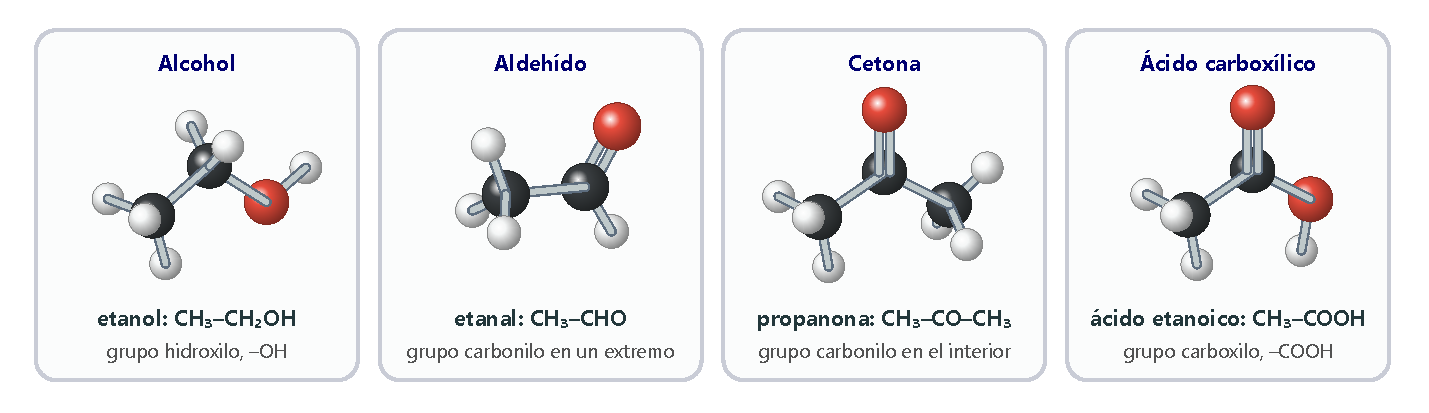
\includegraphics[width=\textwidth]{images/UD4/oxigenados}
    \caption{Modelos moleculares de algunos compuestos oxigenados.}
    \label{fig:oxigenados}
\end{figure}

\subsection{Los alcoholes}

Los \textbf{alcoholes} derivan de los hidrocarburos al sustituir uno o más hidrógenos por \textbf{grupos hidroxilo}, \ch{-OH}, que es su grupo funcional. Se nombran con el prefijo de la cadena principal, el localizador del grupo \ch{-OH} y la terminación \textbf{-ol}:

\begin{center}
    % --- tabla antigua ---
    % \begin{tblr}{colspec={lcl}, hlines, vlines, row{1}={bg=ocre!85, fg=white, font=\bfseries}, cells={font=\small}}
        % Semidesarrollada & Molecular & Nombre \\
        % \ch{CH3OH} & \ch{CH4O} & metanol \\
        % \ch{CH3-CH2OH} & \ch{C2H6O} & etanol \\
        % \ch{CH2OH-CH2-CH3} & \ch{C3H8O} & propan-1-ol \\
        % \ch{CH3-CHOH-CH3} & \ch{C3H8O} & propan-2-ol \\
        % \ch{CH2OH-CH2-CH2-CH3} & \ch{C4H10O} & butan-1-ol \\
    % \end{tblr}
    % --- tabla nueva ---
    {\small
    \begin{tabular}{@{}lcl@{}}
        \toprule
        \textbf{Semidesarrollada} & \textbf{Molecular} & \textbf{Nombre} \\
        \midrule
        \ch{CH3OH} & \ch{CH4O} & metanol \\[3pt]
        \ch{CH3-CH2OH} & \ch{C2H6O} & etanol \\[3pt]
        \ch{CH2OH-CH2-CH3} & \ch{C3H8O} & propan-1-ol \\[3pt]
        \ch{CH3-CHOH-CH3} & \ch{C3H8O} & propan-2-ol \\[3pt]
        \ch{CH2OH-CH2-CH2-CH3} & \ch{C4H10O} & butan-1-ol \\
        \bottomrule
    \end{tabular}
    }
\end{center}

Según el carbono al que esté unido el grupo \ch{-OH}, un alcohol es \textbf{primario} (el carbono está unido a otro carbono), \textbf{secundario} (unido a dos carbonos) o \textbf{terciario} (unido a tres carbonos):
\[ \underset{\text{propan-1-ol (primario)}}{\ch{CH3-CH2-CH2OH}} \qquad \underset{\text{butan-2-ol (secundario)}}{\ch{CH3-CH2-CHOH-CH3}} \qquad \underset{\text{2-metilpropan-2-ol (terciario)}}{\chemfig{CH_3-C(-[2]CH_3)(-[6]CH_3)-OH}} \]

\paragraph{Propiedades.} Los alcoholes tienen puntos de fusión y de ebullición más altos que los hidrocarburos con el mismo número de carbonos. El enlace O--H está polarizado: el hidrógeno tiene una carga parcial positiva (\(\delta+\)) y el oxígeno una negativa (\(\delta-\)), lo que permite que se formen \textbf{enlaces de hidrógeno} entre las moléculas (figura~\ref{fig:enlace_hidrogeno_alcoholes}). Los primeros alcoholes son solubles en agua en cualquier proporción, pero la solubilidad disminuye al crecer la cadena; también se disuelven en disolventes apolares.

\begin{center}
    % --- tabla antigua ---
    % \begin{tblr}{colspec={lc}, hlines, vlines, row{1}={bg=ocre!85, fg=white, font=\bfseries}, cells={font=\small}}
        % Compuesto & \(T_\text{eb}\) (\unit{\degreeCelsius}) \\
        % Metanol & \num{64.5} \\
        % Etanol & \num{78.0} \\
        % Propan-1-ol & \num{97.8} \\
        % Propan-2-ol & \num{82.3} \\
        % Butan-1-ol & \num{117.0} \\
    % \end{tblr}
    % --- tabla nueva ---
    {\small
    \begin{tabular}{@{}lc@{}}
        \toprule
        \textbf{Compuesto} & \textbf{\(T_\text{eb}\) (\unit{\degreeCelsius})} \\
        \midrule
        Metanol & \num{64.5} \\[3pt]
        Etanol & \num{78.0} \\[3pt]
        Propan-1-ol & \num{97.8} \\[3pt]
        Propan-2-ol & \num{82.3} \\[3pt]
        Butan-1-ol & \num{117.0} \\
        \bottomrule
    \end{tabular}
    }
    \qquad
    % --- tabla antigua ---
    % \begin{tblr}{colspec={lc}, hlines, vlines, row{1}={bg=ocre!85, fg=white, font=\bfseries}, cells={font=\small}}
        % Compuesto & \(T_\text{eb}\) (\unit{\degreeCelsius}) \\
        % Propano & \num{-42} \\
        % Butano & \num{-0.5} \\
        % Propanal & \num{49} \\
        % Propanona & \num{56} \\
        % Ácido propanoico & \num{141} \\
    % \end{tblr}
    % --- tabla nueva ---
    {\small
    \begin{tabular}{@{}lc@{}}
        \toprule
        \textbf{Compuesto} & \textbf{\(T_\text{eb}\) (\unit{\degreeCelsius})} \\
        \midrule
        Propano & \num{-42} \\[3pt]
        Butano & \num{-0.5} \\[3pt]
        Propanal & \num{49} \\[3pt]
        Propanona & \num{56} \\[3pt]
        Ácido propanoico & \num{141} \\
        \bottomrule
    \end{tabular}
    }
\end{center}

\begin{figure}[H]
    \centering
    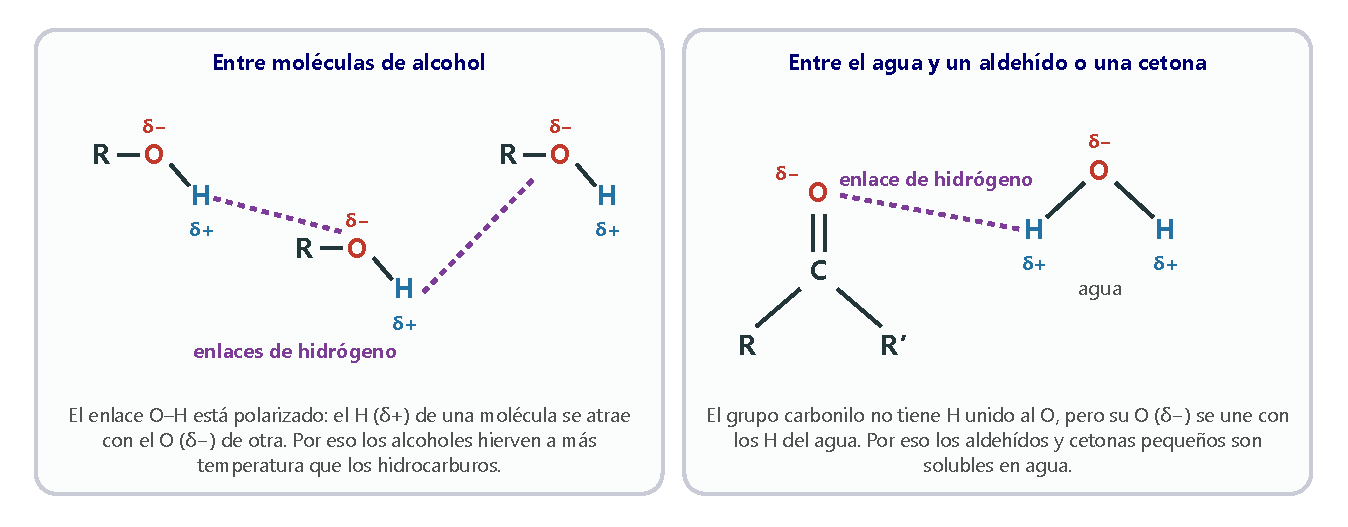
\includegraphics[width=\textwidth]{images/UD4/enlace_hidrogeno}
    \caption{Enlaces de hidrógeno entre moléculas de alcohol y entre el agua y un grupo carbonilo.}
    \label{fig:enlace_hidrogeno_alcoholes}
\end{figure}

\subsection{Los aldehídos y las cetonas}

Los \textbf{aldehídos} y las \textbf{cetonas} tienen el \textbf{grupo carbonilo}, C=O. En los aldehídos está en un \textbf{extremo} de la cadena (\ch{R-CHO}), y en las cetonas, en el \textbf{interior} (\ch{R-CO-R'}).

\paragraph{Nomenclatura.} Los \textbf{aldehídos} se nombran cambiando la -o final del hidrocarburo por \textbf{-al}. La cadena se numera siempre desde el carbono del grupo \ch{-CHO}, así que no hace falta indicar su posición; si hay dos grupos aldehído, se usa \textbf{-dial}. Por ejemplo, \ch{CH3-CH2-CH2-CHO} es el \textbf{butanal} y \ch{CHO-CH2-CH2-CHO}, el \textbf{butanodial}.

Las \textbf{cetonas} se nombran con la terminación \textbf{-ona}, indicando la posición del grupo carbonilo con el localizador más bajo posible: \ch{CH3-CO-CH2-CH3} es la \textbf{butanona}; \ch{CH3-CO-CH2-CH2-CH3}, la \textbf{pentan-2-ona}, y \ch{CH3-CH2-CO-CH2-CH3}, la \textbf{pentan-3-ona}. La cetona más sencilla es la propanona, o \textbf{acetona}, que se usa como disolvente (por ejemplo, en los quitaesmaltes).

\paragraph{Propiedades.} El grupo carbonilo es polar, por lo que los aldehídos y las cetonas hierven a más temperatura que los compuestos apolares de masa parecida. Sin embargo, como no tienen hidrógenos unidos al oxígeno, \textbf{no forman enlaces de hidrógeno entre sus moléculas}, y por eso hierven a menos temperatura que los alcoholes con el mismo número de carbonos. Sí pueden formar enlaces de hidrógeno con el agua (figura~\ref{fig:enlace_hidrogeno_alcoholes}), así que los que tienen pocos carbonos son solubles en agua; también se disuelven en disolventes apolares.

\subsection{Los ácidos carboxílicos y los ésteres}

Los \textbf{ácidos carboxílicos} tienen el \textbf{grupo carboxilo}, \ch{-COOH}, que siempre está en un extremo de la cadena (o en los dos). Se nombran con la palabra \emph{ácido} y la terminación \textbf{-oico}: \ch{HCOOH}, ácido metanoico (fórmico, el de las picaduras de hormiga); \ch{CH3-COOH}, ácido etanoico (acético, el del vinagre); \ch{CH3-CH2-COOH}, ácido propanoico; \ch{CH3-CH2-CH2-COOH}, ácido butanoico.

Los que tienen pocos carbonos son líquidos, y los de más de ocho carbonos son sólidos. Sus puntos de fusión y de ebullición aumentan con el número de carbonos y son los más altos de los compuestos oxigenados, porque forman enlaces de hidrógeno muy fuertes.

Al reaccionar un ácido carboxílico con un alcohol se forma un \textbf{éster} y agua. Los ésteres, con el grupo \ch{-COO\bond{single}}, son responsables del olor y el sabor de muchas frutas y se usan como aromas; por ejemplo, el etanoato de metilo, \ch{CH3-COO-CH3}.

\begin{exercise}
    El etanol es el alcohol más conocido. Busca información sobre sus aplicaciones.
    \begin{solu}
        Respuesta libre. Se usa como \textcolor{red}{desinfectante} (en los geles hidroalcohólicos), como \textcolor{red}{disolvente} (perfumes, medicamentos), como \textcolor{red}{biocombustible} mezclado con la gasolina y está presente en las \textcolor{red}{bebidas alcohólicas}.
    \end{solu}
\end{exercise}

\begin{exercise}
    Formula estos alcoholes y clasifícalos en primarios, secundarios o terciarios: a) butan-1-ol; b) butan-2-ol; c) 2-metilbutan-2-ol.
    \begin{solu}
        a) \ch{CH2OH-CH2-CH2-CH3}, \textcolor{red}{primario}. b) \ch{CH3-CHOH-CH2-CH3}, \textcolor{red}{secundario}.
        c) \[ \chemfig{CH_3-C(-[2]OH)(-[6]CH_3)-CH_2-CH_3} \] \textcolor{red}{terciario}.
    \end{solu}
\end{exercise}

\begin{exercise}
    ¿Cuál es el aldehído más sencillo? ¿Y la cetona más sencilla? Calcula su masa molecular.
    \begin{solu}
        El \textcolor{red}{metanal}, \ch{HCHO} (\ch{CH2O}): \(M = 12 + 2 + 16 = \textcolor{red}{30}\). La \textcolor{red}{propanona}, \ch{CH3-CO-CH3} (\ch{C3H6O}): \(M = 36 + 6 + 16 = \textcolor{red}{58}\).
    \end{solu}
\end{exercise}

\subsection*{Actividades de consolidación: los compuestos oxigenados}

\begin{exercise}
    Vertemos \qty{5}{\mL} de etanol en tres tubos de ensayo. a) Observa el primero: ¿en qué estado está el etanol? ¿Cómo son su color y su olor? b) Al segundo le añadimos agua: ¿es soluble el etanol en agua? c) Al tercero le añadimos un disolvente apolar: ¿es soluble en él?
    \begin{solu}
        a) Es un \textcolor{red}{líquido incoloro} con un \textcolor{red}{olor característico}. b) Es \textcolor{red}{muy soluble} en agua (por su grupo \ch{-OH}). c) También es \textcolor{red}{soluble} en disolventes apolares (por su parte \ch{CH3-CH2\bond{single}}).
    \end{solu}
\end{exercise}

\begin{exercise}
    Formula: a) metanol; b) propan-2-ol; c) butan-1-ol; d) pentan-2-ol.
    \begin{solu}
        a) \textcolor{red}{\ch{CH3OH}}; b) \textcolor{red}{\ch{CH3-CHOH-CH3}};
        c) \textcolor{red}{\ch{CH2OH-CH2-CH2-CH3}}; d) \textcolor{red}{\ch{CH3-CHOH-CH2-CH2-CH3}}.
    \end{solu}
\end{exercise}

\begin{exercise}
    Clasifica estos alcoholes en primarios, secundarios o terciarios:
    \[ \text{a)}\ \chemfig{CH_3-C(-[2]OH)(-[6]CH_3)-CH_2-CH_3} \qquad \text{b)}\ \ch{CH3-CH2OH} \]
    \[ \text{c)}\ \chemfig{CH_3-C(-[2]OH)(-[6]CH_3)-CH_3} \qquad \text{d)}\ \ch{CH3OH} \]
    \begin{solu}
        b) y d) son \textcolor{red}{primarios} (el metanol se considera primario). a) y c) son \textcolor{red}{terciarios}.
    \end{solu}
\end{exercise}

\begin{exercise}
    Indica si son primarios, secundarios o terciarios y escribe su fórmula desarrollada: A: \ch{CH2OH-CH2-CH3}; B: \ch{CH3-CHOH-CH3}.
    \begin{solu}
        A: propan-1-ol, \textcolor{red}{primario}: \[ \chemfig{H-C(-[2]H)(-[6]H)-C(-[2]H)(-[6]H)-C(-[2]H)(-[6]H)-O-H} \]

        B: propan-2-ol, \textcolor{red}{secundario}: \[ \chemfig{H-C(-[2]H)(-[6]H)-C(-[2]OH)(-[6]H)-C(-[2]H)(-[6]H)-H} \]
    \end{solu}
\end{exercise}

\begin{exercise}
    ¿Por qué los alcoholes hierven a mayor temperatura que los hidrocarburos con el mismo número de carbonos? ¿Por qué los primeros alcoholes son solubles en agua?
    \begin{solu}
        Porque el enlace O--H está \textcolor{red}{polarizado} y entre las moléculas de alcohol se forman \textcolor{red}{enlaces de hidrógeno}, que hay que romper para que el líquido hierva. Por la misma razón, el grupo \ch{-OH} forma enlaces de hidrógeno con el agua: los alcoholes de \textcolor{red}{cadena corta} se disuelven en agua en cualquier proporción; al crecer la cadena (parte apolar), la solubilidad disminuye.
    \end{solu}
\end{exercise}

\begin{exercise}
    Formula: a) butanal; b) 2-metilbutanal; c) hexan-3-ona; d) 2-metilpentan-3-ona; e) ácido 3-metilbutanoico; f) ácido 4-metilpentanoico.
    \begin{solu}
        \[ \text{a)}\ \textcolor{red}{\ch{CH3-CH2-CH2-CHO}} \]
        \[ \text{b)}\ \textcolor{red}{\chemfig{CH_3-CH_2-CH(-[6]CH_3)-CHO}} \]
        \[ \text{c)}\ \textcolor{red}{\ch{CH3-CH2-CO-CH2-CH2-CH3}} \]

        \[ \text{d)}\ \textcolor{red}{\chemfig{CH_3-CH(-[6]CH_3)-CO-CH_2-CH_3}} \]
        \[ \text{e)}\ \textcolor{red}{\chemfig{CH_3-CH(-[6]CH_3)-CH_2-COOH}} \]

        \[ \text{f)}\ \textcolor{red}{\chemfig{CH_3-CH(-[6]CH_3)-CH_2-CH_2-COOH}} \]
    \end{solu}
\end{exercise}

\begin{exercise}
    Nombra: a) \ch{CH3-CH2-CH2-COOH}; b) \ch{CH3-CH2-CH2-CH2-CH2-CHO}.
    \begin{solu}
        a) \textcolor{red}{Ácido butanoico}. b) \textcolor{red}{Hexanal}.
    \end{solu}
\end{exercise}

\begin{exercise}
    Señala si es verdadero o falso: a) El butan-2-ol es un alcohol primario. b) El grupo funcional de los aldehídos es \ch{-CHO}. c) Los alcoholes son insolubles en agua. d) El ácido etanoico está en el vinagre.
    \begin{solu}
        a) \textcolor{red}{Falso}: es secundario. b) \textcolor{red}{Verdadero}. c) \textcolor{red}{Falso}: los de cadena corta son muy solubles. d) \textcolor{red}{Verdadero}.
    \end{solu}
\end{exercise}

\begin{exercise}
    Formula: a) etanol; b) ácido etanoico; c) etanal.
    \begin{solu}
        a) \textcolor{red}{\ch{CH3-CH2OH}}; b) \textcolor{red}{\ch{CH3-COOH}}; c) \textcolor{red}{\ch{CH3-CHO}}.
    \end{solu}
\end{exercise}

\begin{exercise}
    Indica si es verdadero o falso y justifica tu respuesta:
    \begin{enumerate}[label=\alph*)]
        \item Los aldehídos y las cetonas hierven a más temperatura que los alcoholes con igual número de carbonos.
        \item Un aldehído o una cetona pueden ser solubles en disolventes polares y apolares.
        \item El grupo carbonilo es el grupo funcional de los ácidos carboxílicos.
        \item El grupo carboxilo es el grupo funcional de las cetonas.
        \item El ácido butanoico hierve a más temperatura que el ácido metanoico.
    \end{enumerate}
    \begin{solu}
        a) \textcolor{red}{Falso}: hierven a menos temperatura, porque no forman enlaces de hidrógeno entre sus moléculas. b) \textcolor{red}{Verdadero}. c) \textcolor{red}{Falso}: es el grupo carboxilo, \ch{-COOH}. d) \textcolor{red}{Falso}: es el grupo carbonilo, C=O. e) \textcolor{red}{Verdadero}: tiene más carbonos.
    \end{solu}
\end{exercise}

%========================================================================================
\section[Las aminas]{¿Qué son los compuestos nitrogenados? Las aminas}
%========================================================================================

Las \textbf{aminas} son compuestos en los que uno, dos o los tres hidrógenos del amoníaco, \ch{NH3}, se sustituyen por cadenas carbonadas. Su grupo funcional es el \textbf{grupo amino}, \ch{-NH2} (figura~\ref{fig:aminas}):
\begin{itemize}
    \item \textbf{Aminas primarias}, \ch{R-NH2}: se sustituye un hidrógeno. Ejemplo: etilamina, \ch{CH3-CH2-NH2}.
    \item \textbf{Aminas secundarias}, \ch{R-NH-R'}: se sustituyen dos hidrógenos. Ejemplo: N-metiletilamina, \ch{CH3-CH2-NH-CH3}.
    \item \textbf{Aminas terciarias}, \ch{RR'R''N}: se sustituyen los tres. Ejemplo: trimetilamina, \ch{N(CH3)3}.
\end{itemize}

\begin{figure}[H]
    \centering
    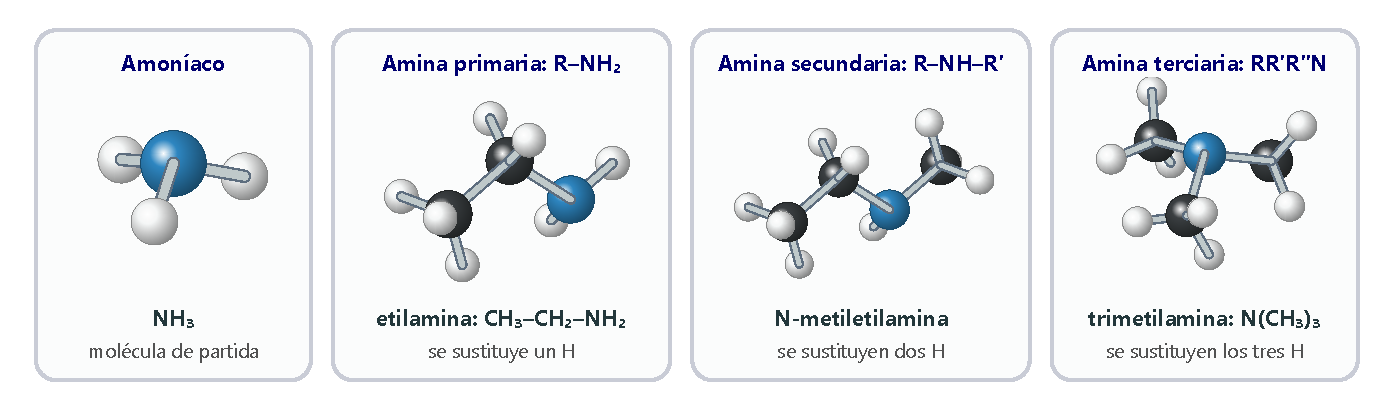
\includegraphics[width=\textwidth]{images/UD4/aminas}
    \caption{Modelos moleculares del amoníaco y de aminas primaria, secundaria y terciaria.}
    \label{fig:aminas}
\end{figure}

\paragraph{Nomenclatura.} Las aminas primarias se nombran añadiendo \textbf{-amina} al nombre del radical: \ch{CH3NH2}, metilamina. En las secundarias y terciarias, se pone \emph{-amina} detrás del radical más largo, y los demás radicales se nombran delante, en orden alfabético y precedidos de \emph{N-} para indicar que están unidos al nitrógeno: \ch{CH3-CH2-CH2-NH-CH3}, N-metilpropilamina; \ch{CH3-CH2-N(CH3)2}, N,N-dimetiletilamina.

\paragraph{Propiedades.} Las aminas primarias y secundarias tienen hidrógenos unidos al nitrógeno y forman enlaces de hidrógeno entre sus moléculas, aunque más débiles que los de los alcoholes. Por eso sus puntos de fusión y de ebullición están entre los de los hidrocarburos y los de los alcoholes de masa parecida. Las aminas de pocos carbonos son muy solubles en agua. Muchas tienen un olor desagradable (a pescado podrido, como la trimetilamina), y forman parte de los aminoácidos y de muchos medicamentos.

\subsection*{Actividades de consolidación: las aminas}

\begin{exercise}
    En la figura~\ref{fig:aminas}, ¿cuántos átomos de carbono están unidos al nitrógeno en cada amina? Relaciónalo con su clasificación.
    \begin{solu}
        En la etilamina, \textcolor{red}{uno} (primaria); en la N-metiletilamina, \textcolor{red}{dos} (secundaria); en la trimetilamina, \textcolor{red}{tres} (terciaria).
    \end{solu}
\end{exercise}

\begin{exercise}
    Formula estas aminas y clasifícalas: a) butilamina; b) N-metilpropilamina; c) N,N-dimetiletilamina; d) N-propilbutilamina.
    \begin{solu}
        a) \ch{CH3-CH2-CH2-CH2-NH2}, \textcolor{red}{primaria}. b) \ch{CH3-CH2-CH2-NH-CH3}, \textcolor{red}{secundaria}. c) \ch{CH3-CH2-N(CH3)2}, \textcolor{red}{terciaria}. d) \ch{CH3-CH2-CH2-CH2-NH-CH2-CH2-CH3}, \textcolor{red}{secundaria}.
    \end{solu}
\end{exercise}

\begin{exercise}
    Nombra la amina \ch{N(CH3)3} y calcula su masa molecular. ¿Es primaria, secundaria o terciaria?
    \begin{solu}
        Es la \textcolor{red}{trimetilamina}, \ch{C3H9N}: \(M = 36 + 9 + 14 = \textcolor{red}{59}\). Es \textcolor{red}{terciaria}.
    \end{solu}
\end{exercise}

\begin{exercise}
    Responde verdadero o falso y justifica tu respuesta: a) En las aminas secundarias se sustituyen dos hidrógenos del amoníaco por dos radicales. b) Las aminas primarias hierven a más temperatura que los hidrocarburos de masa parecida.
    \begin{solu}
        a) \textcolor{red}{Verdadero}. b) \textcolor{red}{Verdadero}: forman \textcolor{red}{enlaces de hidrógeno} entre sus moléculas gracias a los enlaces N--H, que están polarizados.
    \end{solu}
\end{exercise}

%========================================================================================
\section[Compuestos del carbono de especial interés]{¿Qué compuestos del carbono son de especial interés?}
%========================================================================================

Muchos compuestos del carbono tienen interés biológico, industrial o de ambos tipos.

\subsection{Los glúcidos y los lípidos}

Los \textbf{glúcidos} (hidratos de carbono) están formados por carbono, hidrógeno y oxígeno, y los fabrican las plantas verdes mediante la \textbf{fotosíntesis}. Son la principal fuente de energía de los seres vivos: la combustión de cada gramo de glúcidos proporciona al organismo unos \qty{17}{\kilo\joule}. La glucosa y la fructosa están en las frutas y son solubles en agua; la sacarosa (el azúcar común) está formada por una molécula de glucosa y otra de fructosa unidas.

Los \textbf{lípidos} también están formados por carbono, hidrógeno y oxígeno, pero no se disuelven en agua, sino en disolventes apolares. Los más comunes son las grasas, que almacenan más energía por unidad de masa que ningún otro alimento (unos \qty{37}{\kilo\joule\per\gram}). Son ricos en lípidos los aceites, la mantequilla, la nata o la manteca.

\subsection{Los polímeros}

Los \textbf{polímeros} están formados por macromoléculas que resultan de la unión de muchas moléculas pequeñas, los \textbf{monómeros}, en un proceso llamado \textbf{polimerización} (figura~\ref{fig:polietileno}).

\begin{figure}[H]
    \centering
    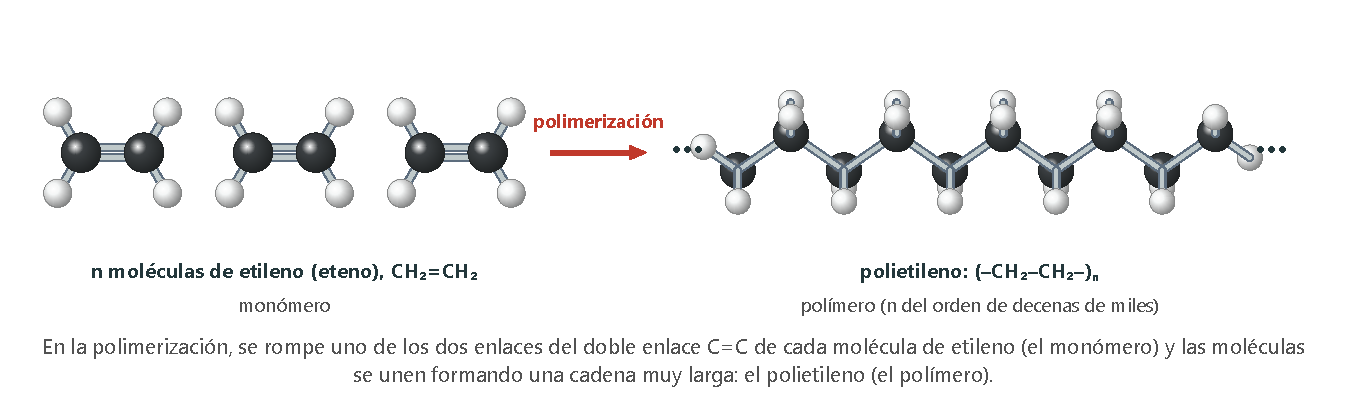
\includegraphics[width=\textwidth]{images/UD4/polietileno}
    \caption{El polietileno se forma por la unión de muchas moléculas de etileno.}
    \label{fig:polietileno}
\end{figure}

\begin{itemize}
    \item \textbf{Polímeros naturales}: el almidón, el glucógeno, la celulosa, las proteínas, los ácidos nucleicos o el caucho. La \textbf{celulosa} es el compuesto del carbono más abundante en la naturaleza; está formada por cadenas de cientos o miles de moléculas de glucosa y es la materia prima del papel y de fibras como el algodón o el lino. El \textbf{caucho} es un polímero del isopreno que se extrae del látex de algunas plantas; se vulcaniza (se calienta con azufre) para que sea más resistente.
    \item \textbf{Polímeros artificiales}: gran parte de la industria química se dedica a fabricar plásticos y fibras artificiales. Se clasifican en:
    \begin{itemize}
        \item \textbf{Termoplásticos}: se reblandecen al calentarlos y recuperan la rigidez al enfriarse, por lo que se pueden moldear y reciclar. Ejemplos: polietileno, poliestireno, PVC, PET.
        \item \textbf{Termoestables}: una vez endurecidos, no se reblandecen al calentarlos. Ejemplos: baquelita, resinas de melamina y epoxi.
        \item \textbf{Elastómeros}: muy elásticos y blandos, formados por cadenas muy largas plegadas sobre sí mismas. Ejemplos: el caucho artificial y el neopreno.
    \end{itemize}
\end{itemize}

\begin{exercise}
    Durante la Primera Guerra Mundial, el caucho natural escaseaba y era carísimo. Científicos estadounidenses y alemanes, de forma independiente, desarrollaron cauchos sintéticos, como el neopreno (1930). Busca información sobre el contexto económico y político de estas investigaciones.
    \begin{solu}
        Respuesta libre. El caucho natural procedía casi todo de plantaciones de Asia controladas por potencias coloniales, y durante las guerras su suministro se cortaba (el bloqueo naval afectó sobre todo a Alemania). Disponer de \textcolor{red}{caucho sintético} se consideraba estratégico para la industria y el ejército (neumáticos, juntas\ldots).
    \end{solu}
\end{exercise}

\subsection*{Actividades de consolidación: compuestos de especial interés}

\begin{exercise}
    ¿Qué son los glúcidos? ¿Qué función tienen en los seres vivos? Nombra algunos y di en qué alimentos se encuentran.
    \begin{solu}
        Son compuestos de \textcolor{red}{carbono, hidrógeno y oxígeno} que constituyen la \textcolor{red}{principal fuente de energía} de los seres vivos. Ejemplos: glucosa y fructosa (frutas, miel), sacarosa (azúcar), almidón (pan, pasta, patatas, arroz).
    \end{solu}
\end{exercise}

\begin{exercise}
    Relaciona cada característica con los glúcidos, los lípidos o ambos: a) solubles en agua; b) insolubles en agua; c) aceites y grasas; d) fuente de energía de los seres vivos; e) formados por C, H y O; f) se obtienen por fotosíntesis.
    \begin{solu}
        a) \textcolor{red}{Glúcidos} (los sencillos); b) \textcolor{red}{lípidos}; c) \textcolor{red}{lípidos}; d) \textcolor{red}{ambos}; e) \textcolor{red}{ambos}; f) \textcolor{red}{glúcidos}.
    \end{solu}
\end{exercise}

\begin{exercise}
    El polietileno tiene la cadena \((\ldots\ch{-CH2-CH2-CH2-CH2-CH2\bond{single}}\ldots)\), con unas \num{100000} unidades \ch{-CH2\bond{single}}. ¿Cuál es su monómero? Si cada molécula de etileno aporta dos unidades, ¿cuántas moléculas de etileno forman una cadena?
    \begin{solu}
        El monómero es el \textcolor{red}{etileno (eteno), \ch{CH2=CH2}}, \ch{C2H4}. Una cadena contiene unas \(\num{100000}/2 = \textcolor{red}{\num{50000}}\) moléculas de etileno.
    \end{solu}
\end{exercise}

\begin{exercise}
    Clasifica en naturales o artificiales: almidón, PVC, celulosa y neopreno.
    \begin{solu}
        Naturales: \textcolor{red}{almidón y celulosa}. Artificiales: \textcolor{red}{PVC y neopreno}.
    \end{solu}
\end{exercise}


%------------------------------------------------


    \chapterimage{images/portada_cabeceras/cabecera_UD5}
    \chapter{La materia y los sistemas materiales}

    %! Author = crist
%! Date = 25/10/2026

\spacing{1.3}
%----------------------------------------------------------------------------------------
%	UNIDAD 5: LA MATERIA Y LOS SISTEMAS MATERIALES (4.º ESO)
%   Figuras: images/UD5/*.pdf (fuente HTML en images/UD5/html, SVG en images/UD5/svg)
%----------------------------------------------------------------------------------------

% Unidades de presión que se usan en la unidad
\DeclareSIUnit\atm{atm}
\DeclareSIUnit\mmHg{mmHg}

% Mapa conceptual del tema (fuente en images/mapas_conceptuales/html/temas.js)
\begin{figure}[H]
    \centering
    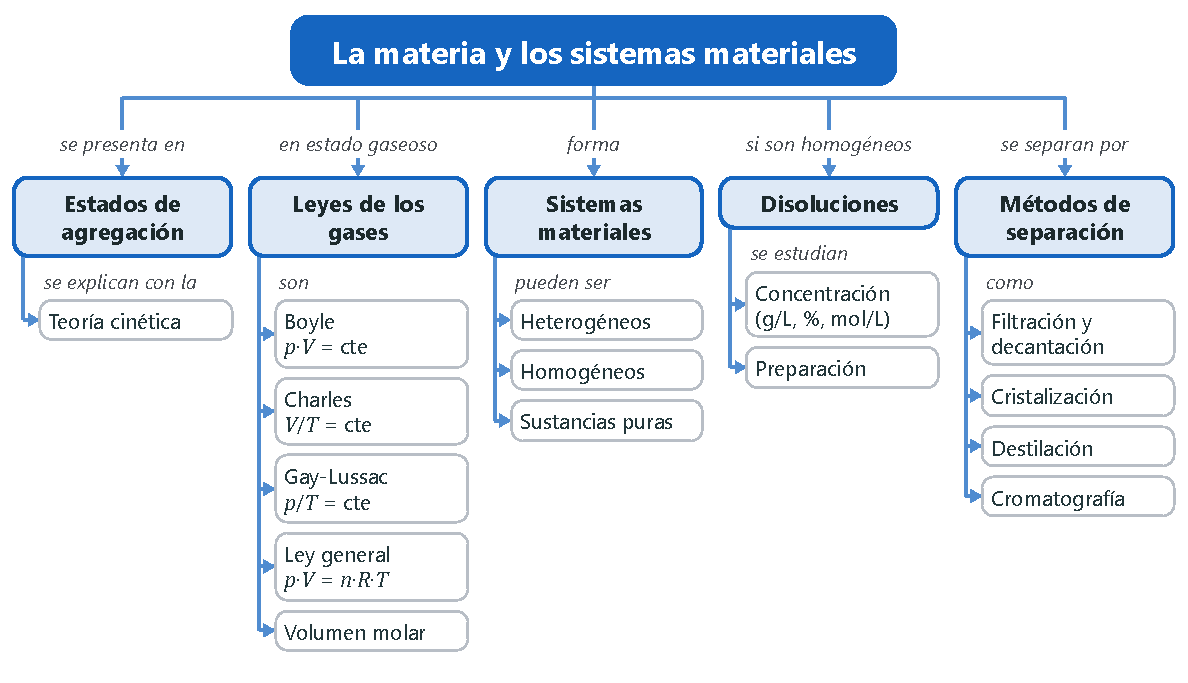
\includegraphics[width=\textwidth]{images/mapas_conceptuales/mapa_UD5}
\end{figure}

%========================================================================================
%\section*{Para empezar: la atmósfera y la capa de ozono}
%\addcontentsline{toc}{section}{Para empezar: la atmósfera y la capa de ozono}
%========================================================================================
%
%La \textbf{atmósfera} es un sistema material gaseoso que contiene los gases imprescindibles para la vida, sobre todo nitrógeno y oxígeno, y en ella tiene lugar el ciclo del agua: evaporación, condensación y precipitación. Aunque el límite científico con el espacio está a unos \qty{104}{\km} de altura, en aviación y astronáutica se toma como frontera la \textbf{línea de Kármán}, a \qty{100}{\km} sobre el nivel del mar.
%
%Entre los 15 y los \qty{50}{\km} de altitud se encuentra la \textbf{capa de ozono}, que reúne el \qty{90}{\percent} del ozono (\ch{O3}) atmosférico y absorbe el \qty{98}{\percent} de la radiación ultravioleta más energética del Sol. Sin ella, esa radiación dañaría a los seres vivos: provoca cáncer de piel, cataratas y otros problemas (figura~\ref{fig:atmosfera_ozono}).
%
%En los años 70 y 80 del siglo pasado se descubrió que el ozono sobre la Antártida estaba disminuyendo. Uno de los principales culpables eran los \textbf{clorofluorocarbonos} (CFC), gases que se usaban en frigoríficos, en la fabricación de espumas y como propelentes de los aerosoles. El agujero cambia de tamaño a lo largo del año y alcanza sus valores mínimos de ozono durante el invierno austral. En 2022 llegó a medir de media unos 23 millones de kilómetros cuadrados, algo menos que el año anterior. Esta mejora se debe, con toda probabilidad, al \textbf{Protocolo de Montreal} (1987), por el que muchos países se comprometieron a dejar de usar los CFC.
%
%\begin{figure}[H]
%    \centering
%    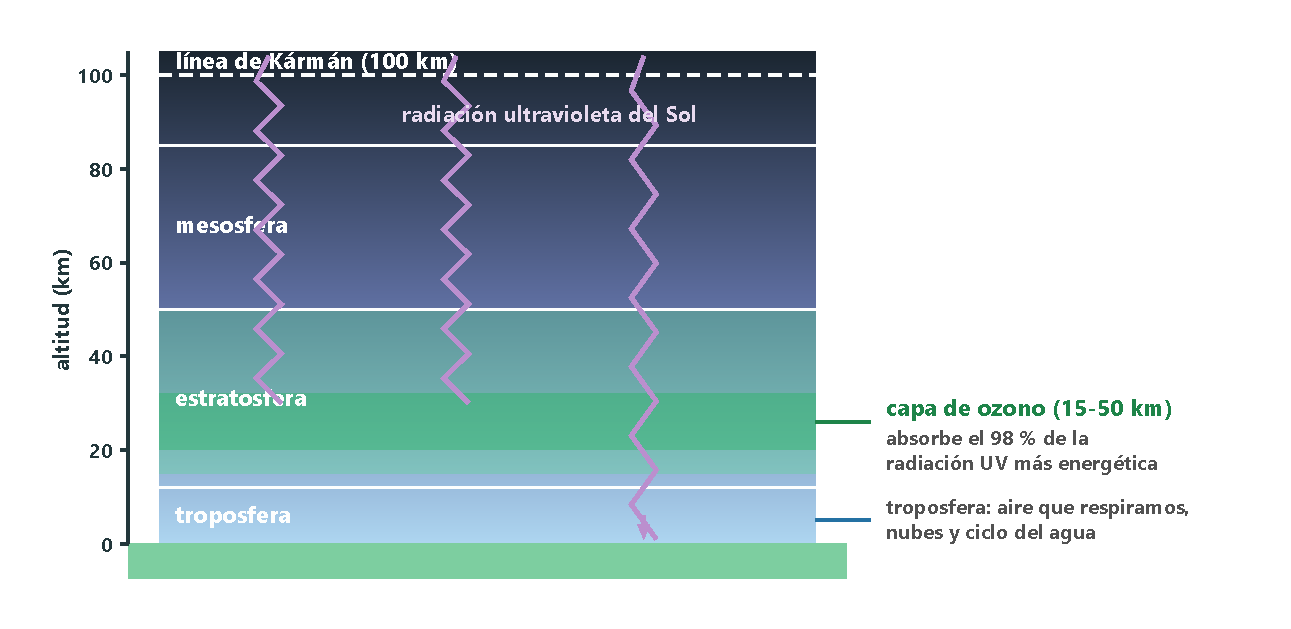
\includegraphics[width=0.85\textwidth]{images/UD5/atmosfera_ozono}
%    \caption{Capas de la atmósfera y situación de la capa de ozono.}
%    \label{fig:atmosfera_ozono}
%\end{figure}
%
%\begin{remark}
%    \textbf{Ozono y Objetivos de Desarrollo Sostenible.} Reducir el agujero de la capa de ozono está relacionado con el \textbf{ODS 3} (\emph{Salud y bienestar}), cuya meta 3.9 pide reducir las muertes y enfermedades causadas por productos químicos peligrosos y por la contaminación del aire, y con el \textbf{ODS 12} (\emph{Producción y consumo responsables}), cuya meta 12.4 busca reducir la liberación de productos químicos a la atmósfera, el agua y el suelo.
%\end{remark}
%
%\begin{exercise}
%    ¿Por qué decimos que la atmósfera es un sistema material gaseoso? ¿Qué papel juega en la existencia de vida en la Tierra?
%    \begin{solu}
%        Porque es una porción de materia formada por \textcolor{red}{gases}. Contiene los gases necesarios para la vida (oxígeno y nitrógeno, principalmente) y en ella se produce el \textcolor{red}{ciclo del agua}: evaporación, condensación y precipitación.
%    \end{solu}
%\end{exercise}
%
%\begin{exercise}
%    ¿Qué es la capa de ozono? ¿A qué altura está y por qué es tan importante para los seres vivos?
%    \begin{solu}
%        Es la zona de la atmósfera, situada entre los \textcolor{red}{15 y los \qty{50}{\km}} de altitud, que contiene el \qty{90}{\percent} del ozono atmosférico. Es importante porque \textcolor{red}{absorbe el \qty{98}{\percent} de la radiación ultravioleta} más energética, que de otro modo produciría cáncer de piel, cataratas y otros daños.
%    \end{solu}
%\end{exercise}
%
%\begin{exercise}
%    ¿Qué sustancias provocaron la aparición del agujero de ozono? ¿En qué época del año es más grande? ¿Por qué fue tan importante el Protocolo de Montreal?
%    \begin{solu}
%        Los \textcolor{red}{clorofluorocarbonos (CFC)}, usados en frigoríficos, espumas y aerosoles. Los valores mínimos de ozono se registran durante el \textcolor{red}{invierno austral} (septiembre y octubre). El Protocolo de Montreal fue un \textcolor{red}{compromiso internacional para dejar de usar los CFC}; gracias a él, el agujero se está reduciendo.
%    \end{solu}
%\end{exercise}
%
%\begin{exercise}
%    Relaciona la reducción del agujero de la capa de ozono con los ODS 3 y 12.
%    \begin{solu}
%        El \textcolor{red}{ODS 3} (meta 3.9) pretende reducir las muertes y enfermedades causadas por productos químicos como los CFC. El \textcolor{red}{ODS 12} (meta 12.4) busca reducir la liberación de productos químicos a la atmósfera.
%    \end{solu}
%\end{exercise}

%========================================================================================
\section{¿Qué es la materia y cómo se presenta?}
%========================================================================================

\begin{definition}[Materia y sustancia]
    La \textbf{materia} es todo aquello que tiene masa y ocupa un volumen. Cada una de las distintas clases de materia es una \textbf{sustancia}.
\end{definition}

La materia se presenta en tres \textbf{estados de agregación}: sólido, líquido y gaseoso. El estado de una sustancia depende de la intensidad de las \textbf{fuerzas de atracción} (o de cohesión) entre sus partículas comparada con su \textbf{movimiento} (vibración o agitación térmica). Recuerda lo que aprendiste sobre el enlace químico en la unidad anterior: el tipo de enlace determina esas fuerzas.

\begin{figure}[H]
    \centering
    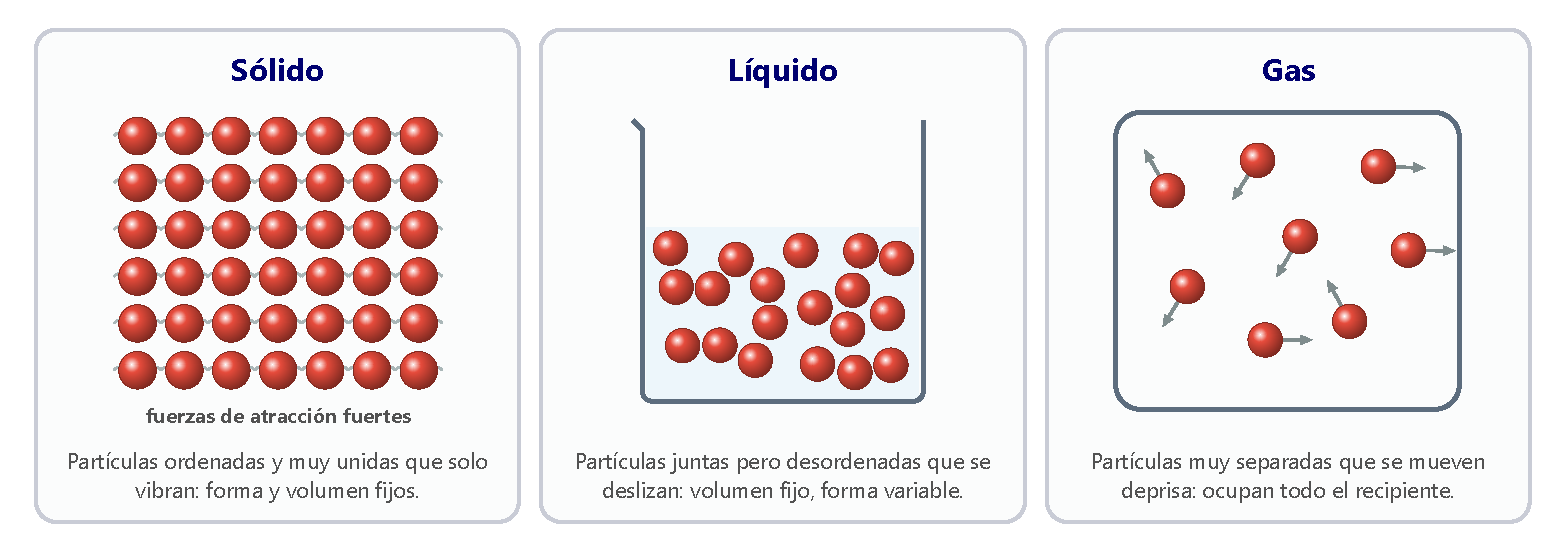
\includegraphics[width=\textwidth]{images/UD5/estados_materia}
    \caption{Modelo de partículas de los tres estados de agregación.}
    \label{fig:estados_materia}
\end{figure}

\begin{itemize}
    \item \textbf{Sólidos.} Las fuerzas de cohesión entre las partículas son mucho más fuertes que su vibración: las partículas ocupan posiciones fijas y el sólido tiene \textbf{forma y volumen propios}. Son sólidos a temperatura ambiente los cristales covalentes (diamante, grafito, \ch{SiO2}), los metales (excepto el mercurio) y los compuestos iónicos como el \ch{NaCl}.
    \item \textbf{Líquidos.} Las fuerzas de cohesión son menores que en los sólidos: las partículas se deslizan unas sobre otras, por eso los líquidos \textbf{fluyen} y se adaptan a la \textbf{forma del recipiente}, aunque su \textbf{volumen no cambia}. El agua (entre 0 y \qty{100}{\celsius}) y el etanol (entre \num{-114} y \qty{78}{\celsius}) son líquidos cuyas moléculas se unen por enlaces de hidrógeno.
    \item \textbf{Gases.} Las fuerzas entre las partículas son muy débiles: se mueven continuamente, de forma desordenada y a gran velocidad, chocando entre sí y con las paredes. Por eso los gases \textbf{ejercen presión}, \textbf{se expanden} hasta ocupar todo el recipiente y \textbf{se pueden comprimir}. Son gases a temperatura ambiente los gases nobles, el \ch{H2}, el \ch{O2}, el \ch{N2}, el \ch{CO2}, el metano o el butano.
\end{itemize}

En los gases, la presión, el volumen y la temperatura están muy relacionados: si cambia una de estas magnitudes, cambian las otras.

\begin{exercise}
    Nombra tres sustancias que sean sólidas, tres líquidas y tres gaseosas a temperatura ambiente. ¿Conoces alguna sustancia que podamos encontrar en la naturaleza en los tres estados?
    \begin{solu}
        Respuesta libre. Sólidos: cloruro de sodio, hierro, diamante. Líquidos: agua, mercurio, etanol. Gases: oxígeno, dióxido de carbono, butano. El \textcolor{red}{agua} se encuentra en la naturaleza como hielo, agua líquida y vapor.
    \end{solu}
\end{exercise}

\begin{exercise}
    Explica, comparando las fuerzas de cohesión con la agitación de las partículas, por qué\ldots
    \begin{enumerate}[label=\alph*)]
        \item un sólido tiene forma y volumen fijos;
        \item un gas tiende a ocupar todo el volumen disponible;
        \item las partículas de un líquido no ocupan posiciones fijas;
        \item un gas ejerce presión sobre las paredes del recipiente;
        \item un líquido fluye y se adapta a la forma del recipiente.
    \end{enumerate}
    \begin{solu}
        a) Las fuerzas de cohesión son \textcolor{red}{mucho mayores} que la vibración de las partículas. b) La agitación de las partículas es \textcolor{red}{mucho mayor} que las fuerzas de cohesión. c) y e) Las fuerzas de cohesión \textcolor{red}{no son tan intensas como en los sólidos}: mantienen las partículas juntas pero les permiten deslizarse. d) Las partículas se mueven muy deprisa y \textcolor{red}{chocan continuamente} contra las paredes.
    \end{solu}
\end{exercise}

\begin{exercise}
    Los gases combustibles más usados son el butano, el propano y el gas natural (metano). En las mismas condiciones, la densidad del aire es \qty{1.3}{\kg\per\cubic\metre}, la del butano \qty{2.6}{\kg\per\cubic\metre}, la del propano \qty{1.9}{\kg\per\cubic\metre} y la del metano \qty{0.7}{\kg\per\cubic\metre}.
    \begin{enumerate}[label=\alph*)]
        \item ¿Dónde se acumula cada gas si hay una fuga?
        \item Busca qué medidas de seguridad se toman en los lugares donde se usan estos gases.
    \end{enumerate}
    \begin{solu}
        a) El butano y el propano son \textcolor{red}{más densos que el aire}: se acumulan \textcolor{red}{cerca del suelo}. El metano es menos denso: \textcolor{red}{sube y se acumula cerca del techo}.
        b) Respuesta libre: rejillas de ventilación a ras de suelo (butano, propano) o en la parte alta (gas natural), detectores de gas, revisiones periódicas de la instalación, no hacer chispas ni encender interruptores si se nota olor a gas\ldots
    \end{solu}
\end{exercise}

\begin{exercise}
    Se coloca un globo desinflado en la boca de un matraz con agua y se añade una pastilla efervescente. Explica lo que le sucede al globo.
    \begin{solu}
        La pastilla desprende un gas (\ch{CO2}). Los gases tienen masa y ocupan un volumen, y su volumen es variable: el gas \textcolor{red}{se expande} y ejerce presión sobre las paredes del globo, que \textcolor{red}{se infla}.
    \end{solu}
\end{exercise}

\begin{exercise}
    ¿Pueden estar dos gases en el mismo recipiente sin mezclarse? Razona tu respuesta.
    \begin{solu}
        \textcolor{red}{No}. Las partículas de los gases se mueven continuamente y en todas direcciones, de modo que \textcolor{red}{se difunden} y acaban mezclándose en todo el recipiente.
    \end{solu}
\end{exercise}

%========================================================================================
\section{¿Qué leyes rigen el comportamiento de los gases?}
%========================================================================================

Vamos a estudiar cómo se relacionan la \textbf{presión} (\(p\)), el \textbf{volumen} (\(V\)) y la \textbf{temperatura} (\(T\)) de una misma masa de gas encerrada en un recipiente. En todas las leyes de los gases la temperatura se expresa en \textbf{kelvin}: \(T\,(\unit{\kelvin}) = t\,(\unit{\celsius}) + 273\). La presión puede medirse en atmósferas, en milímetros de mercurio o en pascales: \(\qty{1}{\atm} = \qty{760}{\mmHg} = \qty{101325}{\pascal}\).

\begin{figure}[H]
    \centering
    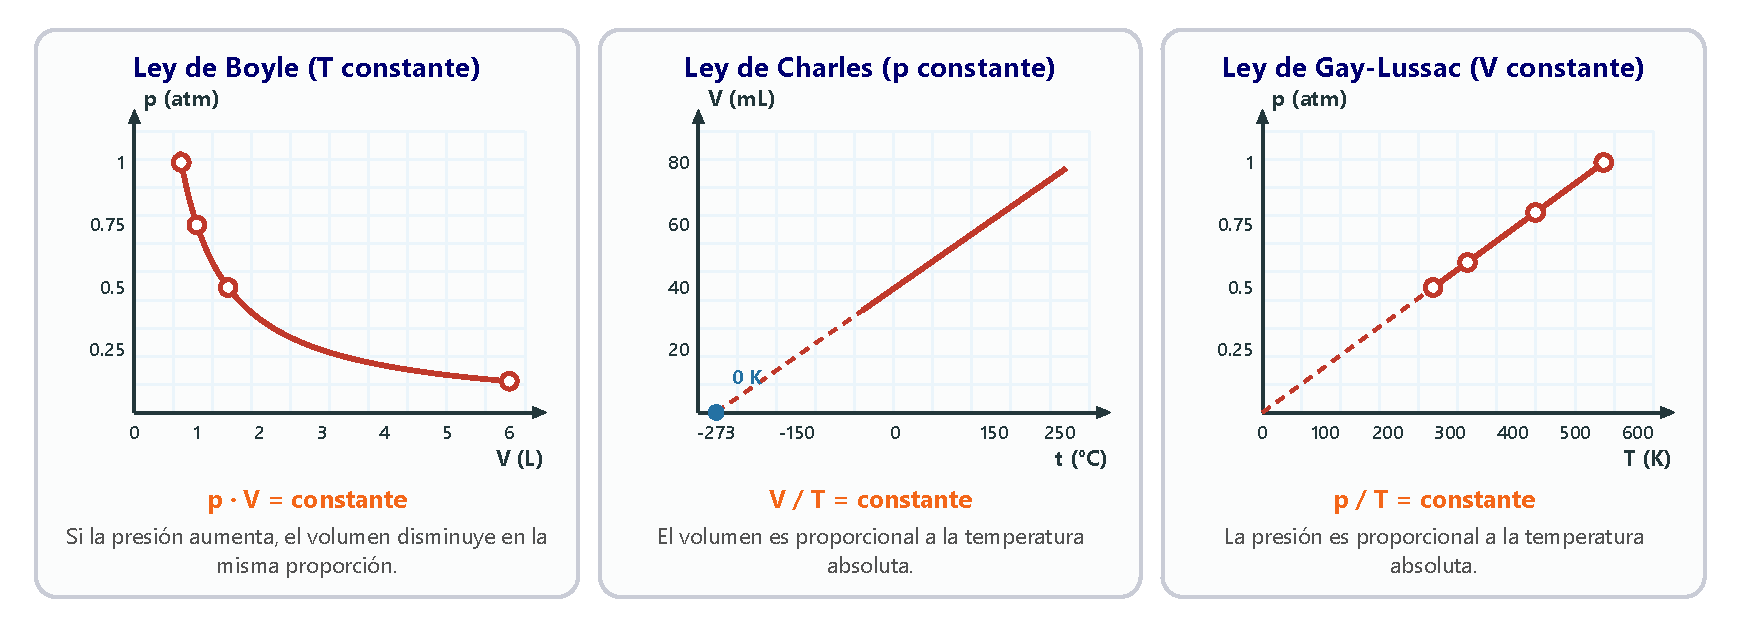
\includegraphics[width=\textwidth]{images/UD5/leyes_gases}
    \caption{Gráficas de las leyes de Boyle, Charles y Gay-Lussac.}
    \label{fig:leyes_gases}
\end{figure}

\subsection{Presión y volumen a temperatura constante: ley de Boyle}

Encerramos un gas en un cilindro con un émbolo móvil y un manómetro, y mantenemos la temperatura constante con un termostato. Al mover el émbolo obtenemos:

\begin{center}
    % --- tabla antigua ---
    % \begin{tblr}{colspec={lcccc}, hlines, vlines, column{1}={bg=ocre!85, fg=white, font=\bfseries}}
        % \(p\) (\unit{\atm}) & \num{1.000} & \num{0.750} & \num{0.500} & \num{0.125} \\
        % \(V\) (\unit{\L}) & \num{0.750} & \num{1.000} & \num{1.500} & \num{6.000} \\
        % \(p \cdot V\) (\unit{\atm\cdot\L}) & \num{0.750} & \num{0.750} & \num{0.750} & \num{0.750} \\
    % \end{tblr}
    % --- tabla nueva ---
    \begin{tabular}{@{}lcccc@{}}
        \toprule
        \textbf{\(p\) (\unit{\atm})} & \num{1.000} & \num{0.750} & \num{0.500} & \num{0.125} \\[3pt]
        \textbf{\(V\) (\unit{\L})} & \num{0.750} & \num{1.000} & \num{1.500} & \num{6.000} \\[3pt]
        \textbf{\(p \cdot V\) (\unit{\atm\cdot\L})} & \num{0.750} & \num{0.750} & \num{0.750} & \num{0.750} \\
        \bottomrule
    \end{tabular}
\end{center}

El producto \(p \cdot V\) es siempre el mismo. Robert Boyle (1662) y, de forma independiente, Edme Mariotte llegaron a esta conclusión:

\begin{definition}[Ley de Boyle-Mariotte]
    A temperatura constante, el volumen de una masa de gas es \textbf{inversamente proporcional} a la presión:
    \[ p \cdot V = \text{constante} \qquad\Rightarrow\qquad p_1 \cdot V_1 = p_2 \cdot V_2 \]
\end{definition}

\begin{example}
    Una bombona de \qty{20}{\L} contiene aire a \qty{12}{\atm}. ¿Qué volumen ocuparía ese aire a \qty{1}{\atm} y a la misma temperatura?

    \textcolor{blue}{Datos:} \(p_1 = \qty{12}{\atm}\); \(V_1 = \qty{20}{\L}\); \(p_2 = \qty{1}{\atm}\).
    \[ p_1 V_1 = p_2 V_2 \;\Rightarrow\; V_2 = \frac{p_1 V_1}{p_2} = \frac{\qty{12}{\atm} \cdot \qty{20}{\L}}{\qty{1}{\atm}} = \textcolor{red}{\qty{240}{\L}} \]
\end{example}

\subsection{Volumen y temperatura a presión constante: ley de Charles}

Si calentamos un gas encerrado en un cilindro con un émbolo que se mueve libremente (la presión no cambia), el gas \textbf{se dilata}, mucho más que los sólidos y los líquidos. Si representamos el volumen frente a la temperatura en grados Celsius obtenemos una recta que, prolongada, corta el eje de temperaturas en \qty{-273}{\celsius}: el \textbf{cero absoluto} (\qty{0}{\kelvin}) (figura~\ref{fig:leyes_gases}).

\begin{definition}[Ley de Charles]
    A presión constante, el volumen de una masa de gas es \textbf{directamente proporcional} a su temperatura absoluta:
    \[ \frac{V}{T} = \text{constante} \qquad\Rightarrow\qquad \frac{V_1}{T_1} = \frac{V_2}{T_2} \]
\end{definition}

\subsection{Presión y temperatura a volumen constante: ley de Gay-Lussac}

Ahora encerramos el gas en un recipiente rígido con un manómetro y lo calentamos al baño María, midiendo la temperatura con un termómetro:

\begin{center}
    % --- tabla antigua ---
    % \begin{tblr}{colspec={cccc}, hlines, vlines, row{1}={bg=ocre!85, fg=white, font=\bfseries}}
        % Experiencia & \(p\) (\unit{\atm}) & \(T\) (\unit{\kelvin}) & \(p/T\) (\unit{\atm\per\kelvin}) \\
        % 1 & \num{0.5} & 273 & \num{1.83e-3} \\
        % 2 & \num{0.6} & 328 & \num{1.83e-3} \\
        % 3 & \num{0.8} & 437 & \num{1.83e-3} \\
        % 4 & \num{1.0} & 546 & \num{1.83e-3} \\
    % \end{tblr}
    % --- tabla nueva ---
    \begin{tabular}{@{}cccc@{}}
        \toprule
        \textbf{Experiencia} & \textbf{\(p\) (\unit{\atm})} & \textbf{\(T\) (\unit{\kelvin})} & \textbf{\(p/T\) (\unit{\atm\per\kelvin})} \\
        \midrule
        1 & \num{0.5} & 273 & \num{1.83e-3} \\[3pt]
        2 & \num{0.6} & 328 & \num{1.83e-3} \\[3pt]
        3 & \num{0.8} & 437 & \num{1.83e-3} \\[3pt]
        4 & \num{1.0} & 546 & \num{1.83e-3} \\
        \bottomrule
    \end{tabular}
\end{center}

\begin{definition}[Ley de Gay-Lussac]
    A volumen constante, la presión de una masa de gas es \textbf{directamente proporcional} a su temperatura absoluta:
    \[ \frac{p}{T} = \text{constante} \qquad\Rightarrow\qquad \frac{p_1}{T_1} = \frac{p_2}{T_2} \]
\end{definition}

\begin{example}
    Un depósito contiene un gas a \qty{2}{\atm} y \qty{15}{\celsius}. Su válvula de seguridad se abre cuando la presión llega a \qty{6}{\atm}. ¿A qué temperatura se abrirá?

    \textcolor{blue}{Datos:} \(p_1 = \qty{2}{\atm}\); \(T_1 = 15 + 273 = \qty{288}{\kelvin}\); \(p_2 = \qty{6}{\atm}\).
    \[ \frac{p_1}{T_1} = \frac{p_2}{T_2} \;\Rightarrow\; T_2 = \frac{p_2 \, T_1}{p_1} = \frac{6 \cdot 288}{2} = \textcolor{red}{\qty{864}{\kelvin}} \;(\qty{591}{\celsius}) \]
\end{example}

\begin{exercise}
    ¿Qué le ocurre a un globo lleno de aire si lo metemos en el frigorífico? ¿Qué ley lo explica?
    \begin{solu}
        Al cabo de un tiempo \textcolor{red}{su volumen disminuye}, porque baja la temperatura del aire de su interior (a presión prácticamente constante). Lo explica la \textcolor{red}{ley de Charles}.
    \end{solu}
\end{exercise}

\begin{exercise}
    ¿Cómo cambia el volumen de un gas a temperatura constante si su presión se reduce a la mitad?
    \begin{solu}
        Como \(p \cdot V\) es constante, si la presión se reduce a la mitad \textcolor{red}{el volumen se duplica}.
    \end{solu}
\end{exercise}

\begin{exercise}
    ¿Cómo cambia el volumen de un gas a presión constante si su temperatura absoluta se triplica? ¿Y si lo que se triplica es su temperatura en grados Celsius?
    \begin{solu}
        Si se triplica la temperatura \textbf{absoluta}, \textcolor{red}{el volumen se triplica} (ley de Charles). Si se triplica la temperatura en \unit{\celsius}, el volumen \textcolor{red}{no} se triplica, porque la ley solo se cumple con temperaturas en kelvin.
    \end{solu}
\end{exercise}

\begin{exercise}
    ¿Qué le ocurre a la presión de un gas encerrado en un recipiente rígido si su temperatura absoluta se reduce a la mitad?
    \begin{solu}
        Según la ley de Gay-Lussac, \textcolor{red}{la presión también se reduce a la mitad}.
    \end{solu}
\end{exercise}

\begin{exercise}
    Un recipiente cerrado contiene un gas a \qty{1.20}{\atm} y \qty{20}{\celsius}.
    \begin{enumerate}[label=\alph*)]
        \item ¿Qué presión habrá si se calienta hasta \qty{50}{\celsius}?
        \item Copia y completa la tabla para otro gas del mismo tipo de experiencia:
        \begin{center}
            % --- tabla antigua ---
            % \begin{tblr}{colspec={lccc}, hlines, vlines, column{1}={bg=ocre!85, fg=white, font=\bfseries}}
                % \(p\) (\unit{\atm}) & \num{1.00} & \ldots & \num{1.50} \\
                % \(T\) (\unit{\kelvin}) & 293 & 373 & \ldots \\
            % \end{tblr}
            % --- tabla nueva ---
            \begin{tabular}{@{}lccc@{}}
                \toprule
                \textbf{\(p\) (\unit{\atm})} & \num{1.00} & \ldots & \num{1.50} \\[3pt]
                \textbf{\(T\) (\unit{\kelvin})} & 293 & 373 & \ldots \\
                \bottomrule
            \end{tabular}
        \end{center}
        \item Representa gráficamente los datos de la tabla.
    \end{enumerate}
    \begin{solu}
        a) \(T_1 = \qty{293}{\kelvin}\); \(T_2 = \qty{323}{\kelvin}\). \(p_2 = p_1 \dfrac{T_2}{T_1} = \num{1.20} \cdot \dfrac{323}{293} = \textcolor{red}{\qty{1.32}{\atm}}\).
        b) \(p = \num{1.00} \cdot \frac{373}{293} = \textcolor{red}{\qty{1.27}{\atm}}\); \(T = 293 \cdot \frac{\num{1.50}}{\num{1.00}} = \textcolor{red}{\qty{439.5}{\kelvin}}\).
        c) Los puntos están sobre una \textcolor{red}{recta que pasa por el origen}, como en la figura~\ref{fig:leyes_gases}.
    \end{solu}
\end{exercise}

\subsection{La ley combinada de los gases ideales}

¿Qué pasa si cambian a la vez la presión, el volumen y la temperatura? Podemos imaginar que el gas pasa del estado inicial (\(p_1\), \(V_1\), \(T_1\)) al final (\(p_2\), \(V_2\), \(T_2\)) en dos etapas (figura~\ref{fig:ley_combinada}):

\begin{enumerate}[label=\numberballblue]
    \item A temperatura constante, la presión pasa de \(p_1\) a \(p_2\) y el volumen de \(V_1\) a un valor intermedio \(V'\). Por la ley de Boyle: \(p_1 V_1 = p_2 V'\).
    \item A presión constante, la temperatura pasa de \(T_1\) a \(T_2\) y el volumen de \(V'\) a \(V_2\). Por la ley de Charles: \(V'/T_1 = V_2/T_2\).
\end{enumerate}

Despejando \(V'\) en las dos expresiones e igualando se obtiene la \textbf{ley combinada de los gases ideales}:

\begin{centeredequation}
    \frac{p_1 \cdot V_1}{T_1} = \frac{p_2 \cdot V_2}{T_2}
\end{centeredequation}

\begin{figure}[H]
    \centering
    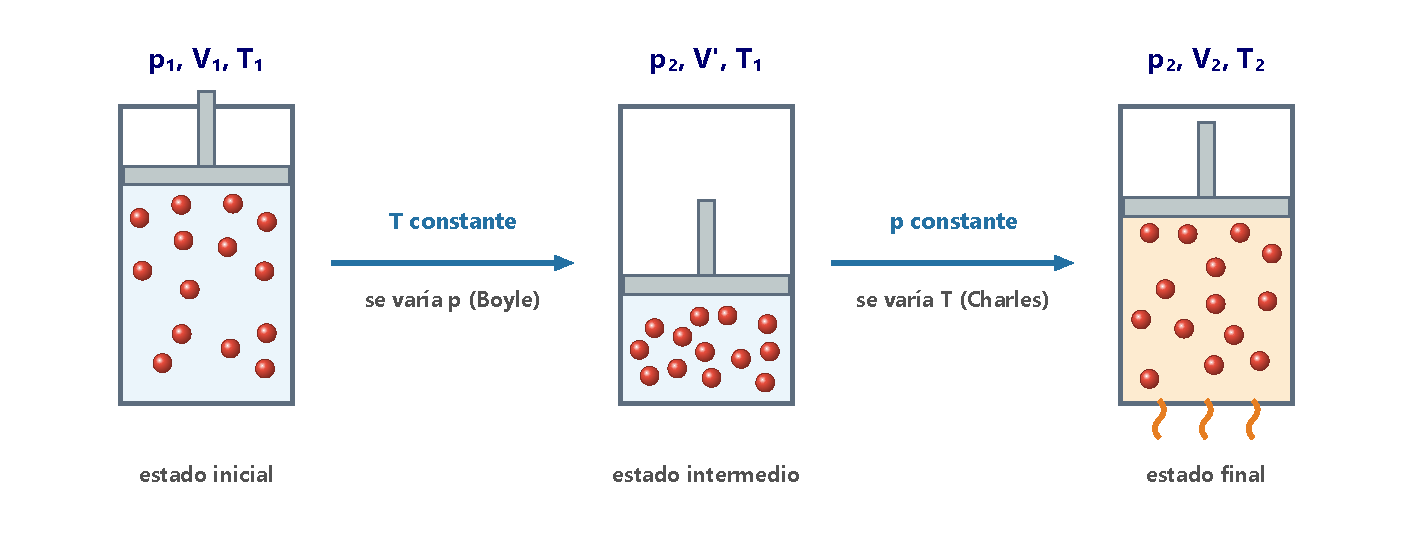
\includegraphics[width=0.85\textwidth]{images/UD5/ley_combinada}
    \caption{Paso de un estado a otro en dos etapas: primero a temperatura constante y después a presión constante.}
    \label{fig:ley_combinada}
\end{figure}

Si la cantidad de gas no cambia, el cociente \(p \cdot V / T\) es constante: si fijamos dos de las tres variables, la tercera queda determinada. Al aplicar la ley hay que tener en cuenta que:
\begin{enumerate}[label=\arabic*.]
    \item A cada lado de la igualdad deben usarse las \textbf{mismas unidades} de presión y de volumen.
    \item La temperatura siempre se expresa en \textbf{kelvin}.
\end{enumerate}

\begin{example}
    Un gas ocupa \qty{12}{\L} a \qty{27}{\celsius} y \qty{1}{\atm}. ¿Qué volumen ocupará a \qty{127}{\celsius} y \qty{2}{\atm}?

    \textcolor{blue}{Datos:} \(V_1 = \qty{12}{\L}\); \(p_1 = \qty{1}{\atm}\); \(T_1 = \qty{300}{\kelvin}\); \(p_2 = \qty{2}{\atm}\); \(T_2 = \qty{400}{\kelvin}\).
    \[ \frac{p_1 V_1}{T_1} = \frac{p_2 V_2}{T_2} \;\Rightarrow\; V_2 = \frac{p_1 V_1 T_2}{T_1 \, p_2} = \frac{1 \cdot 12 \cdot 400}{300 \cdot 2} = \textcolor{red}{\qty{8}{\L}} \]
\end{example}

\begin{exercise}
    Un gas a \qty{20}{\celsius} y \qty{1}{\atm} ocupa \qty{20}{\L}. Si al calentarlo hasta \qty{60}{\celsius} pasa a ocupar \qty{30}{\L}, ¿a qué presión estará?
    \begin{solu}
        \(T_1 = \qty{293}{\kelvin}\); \(T_2 = \qty{333}{\kelvin}\).
        \[ p_2 = \frac{p_1 V_1 T_2}{T_1 V_2} = \frac{1 \cdot 20 \cdot 333}{293 \cdot 30} = \textcolor{red}{\qty{0.76}{\atm}} \]
    \end{solu}
\end{exercise}

\begin{exercise}
    Indica si son verdaderas o falsas estas afirmaciones y corrige las falsas:
    \begin{enumerate}[label=\alph*)]
        \item Según la ley de Boyle, a temperatura constante el volumen de un gas es directamente proporcional a la presión.
        \item A presión constante, el volumen de un gas es directamente proporcional a su temperatura en kelvin.
        \item El cero de la escala Kelvin corresponde a \qty{-273.15}{\celsius}.
    \end{enumerate}
    \begin{solu}
        a) \textcolor{red}{Falsa}: el volumen es \emph{inversamente} proporcional a la presión. b) \textcolor{red}{Verdadera} (ley de Charles). c) \textcolor{red}{Verdadera}.
    \end{solu}
\end{exercise}

\begin{exercise}
    Lee el texto y contesta:

    \begin{quote}
        \emph{La presión de los neumáticos de una moto es esencial: si van demasiado blandos, la rueda se desgasta antes y, en la delantera, la frenada empeora. Un aumento del \qty{10}{\percent} de la temperatura del aire de la rueda aumenta un \qty{10}{\percent} su presión. La presión se suele dar en bar (\(\qty{1}{\atm} = \qty{1.013}{\bar}\)). Se recomienda llevar la rueda delantera a \qty{2.2}{\bar} y la trasera a \qty{2.4}{\bar}, medidas en frío con un manómetro. Si se mide en caliente, hay que sumar \qty{0.3}{\bar} a la presión aconsejada.}
    \end{quote}

    \begin{enumerate}[label=\alph*)]
        \item Expresa en atm y en mmHg las presiones recomendadas.
        \item ¿Por qué es peligroso llevar los neumáticos con menos presión de la indicada?
        \item ¿Qué precauciones hay que tener al medir la presión?
        \item ¿Qué le pasa a la presión del aire si aumenta la temperatura? ¿Qué ley lo explica?
        \item Tras circular una hora, la rueda delantera marca \qty{2.5}{\bar} y la trasera \qty{2.7}{\bar}. ¿Es correcta la presión?
    \end{enumerate}
    \begin{solu}
        a) Delantera: \(\frac{\num{2.2}}{\num{1.013}} = \qty{2.17}{\atm}\); \(\num{2.17} \cdot 760 = \textcolor{red}{\qty{1650}{\mmHg}}\). Trasera: \(\frac{\num{2.4}}{\num{1.013}} = \qty{2.37}{\atm}\); \(\num{2.37} \cdot 760 = \textcolor{red}{\qty{1801}{\mmHg}}\).
        b) Se desgasta antes la banda de rodadura y la frenada es peor.
        c) Medirla en frío o, si se mide en caliente, sumar \qty{0.3}{\bar} a la presión aconsejada.
        d) \textcolor{red}{Aumenta} (ley de Gay-Lussac: el volumen de la rueda es casi constante).
        e) \textcolor{red}{Sí}: en caliente deberían marcar \(\num{2.2} + \num{0.3} = \qty{2.5}{\bar}\) y \(\num{2.4} + \num{0.3} = \qty{2.7}{\bar}\).
    \end{solu}
\end{exercise}

\begin{exercise}
    ¿A qué presión hay que someter \qty{3}{\L} de nitrógeno que están a \qty{1.2}{\atm} para comprimirlos hasta \qty{0.9}{\L} sin cambiar la temperatura? ¿Qué ley has aplicado?
    \begin{solu}
        Ley de \textcolor{red}{Boyle}: \(p_2 = \dfrac{p_1 V_1}{V_2} = \dfrac{\num{1.2} \cdot 3}{\num{0.9}} = \textcolor{red}{\qty{4}{\atm}}\).
    \end{solu}
\end{exercise}

\begin{exercise}
    Tenemos \qty{40}{\cubic\centi\metre} de oxígeno a \qty{760}{\mmHg}. ¿Qué volumen ocupará a \qty{640}{\mmHg} si la temperatura no cambia?
    \begin{solu}
        \(V_2 = \dfrac{p_1 V_1}{p_2} = \dfrac{760 \cdot 40}{640} = \textcolor{red}{\qty{47.5}{\cubic\centi\metre}}\).
    \end{solu}
\end{exercise}

\begin{exercise}
    Un cilindro con un émbolo móvil contiene \qty{30}{\cubic\centi\metre} de gas a \qty{27}{\celsius}. Si el volumen máximo del cilindro es \qty{75}{\cubic\centi\metre}, ¿hasta qué temperatura se puede calentar a presión constante? ¿Qué ley has usado?
    \begin{solu}
        Ley de \textcolor{red}{Charles}, con \(T_1 = \qty{300}{\kelvin}\):
        \(T_2 = T_1 \dfrac{V_2}{V_1} = 300 \cdot \dfrac{75}{30} = \textcolor{red}{\qty{750}{\kelvin}} = \qty{477}{\celsius}\).
    \end{solu}
\end{exercise}

\begin{exercise}
    Un gas ocupa \qty{12}{\cubic\deci\metre} a \qty{0}{\celsius} y \qty{1}{\atm}. ¿Qué volumen ocupará a \qty{50}{\celsius} si la presión no cambia?
    \begin{solu}
        \(V_2 = V_1 \dfrac{T_2}{T_1} = 12 \cdot \dfrac{323}{273} = \textcolor{red}{\qty{14.2}{\cubic\deci\metre}}\).
    \end{solu}
\end{exercise}

\begin{exercise}
    Escribe cómo queda la ley combinada de los gases si a) la presión es constante; b) la temperatura es constante; c) el volumen es constante. ¿Qué nombre recibe cada una?
    \begin{solu}
        a) \(\dfrac{V_1}{T_1} = \dfrac{V_2}{T_2}\): \textcolor{red}{ley de Charles}. b) \(p_1 V_1 = p_2 V_2\): \textcolor{red}{ley de Boyle-Mariotte}. c) \(\dfrac{p_1}{T_1} = \dfrac{p_2}{T_2}\): \textcolor{red}{ley de Gay-Lussac}.
    \end{solu}
\end{exercise}

\begin{exercise}
    Una masa de oxígeno ocupa \qty{25}{\cubic\deci\metre} a \qty{27}{\celsius} y \qty{760}{\mmHg}. ¿Qué volumen ocupará a \qty{87}{\celsius} y \qty{950}{\mmHg}?
    \begin{solu}
        \(T_1 = \qty{300}{\kelvin}\); \(T_2 = \qty{360}{\kelvin}\).
        \[ V_2 = \frac{p_1 V_1 T_2}{T_1 \, p_2} = \frac{760 \cdot 25 \cdot 360}{300 \cdot 950} = \textcolor{red}{\qty{24}{\cubic\deci\metre}} \]
    \end{solu}
\end{exercise}

\begin{exercise}
    Un gas ocupa \qty{3}{\cubic\deci\metre} a \qty{27}{\celsius} y \qty{1}{\atm}. Lo calentamos hasta \qty{54}{\celsius}.
    \begin{enumerate}[label=\alph*)]
        \item Si la presión no cambia, ¿qué volumen ocupará? ¿Se ha duplicado el volumen al duplicar la temperatura en grados Celsius?
        \item Si el volumen no cambia, ¿qué presión tendrá? ¿Se ha duplicado?
    \end{enumerate}
    \begin{solu}
        \(T_1 = \qty{300}{\kelvin}\); \(T_2 = \qty{327}{\kelvin}\).
        a) \(V_2 = 3 \cdot \frac{327}{300} = \textcolor{red}{\qty{3.27}{\cubic\deci\metre}}\). \textcolor{red}{No} se duplica: la proporcionalidad es con la temperatura en kelvin.
        b) \(p_2 = 1 \cdot \frac{327}{300} = \textcolor{red}{\qty{1.09}{\atm}}\). Tampoco se duplica.
    \end{solu}
\end{exercise}

\begin{exercise}
    El aire de los neumáticos de un coche está a \qty{15}{\celsius} y \qty{2.2}{\atm}. Calcula su presión cuando, por el rozamiento con el asfalto, su temperatura llega a \qty{45}{\celsius}.
    \begin{solu}
        \(p_2 = p_1 \dfrac{T_2}{T_1} = \num{2.2} \cdot \dfrac{318}{288} = \textcolor{red}{\qty{2.43}{\atm}}\).
    \end{solu}
\end{exercise}

\begin{exercise}
    Un gas encerrado por un émbolo móvil ocupa \qty{40}{\L} a \qty{27}{\celsius} y \qty{4}{\atm}. ¿Qué volumen ocupará a \qty{1}{\atm} y \qty{0}{\celsius}?
    \begin{solu}
        \(V_2 = \dfrac{p_1 V_1 T_2}{T_1 \, p_2} = \dfrac{4 \cdot 40 \cdot 273}{300 \cdot 1} = \textcolor{red}{\qty{145.6}{\L}}\).
    \end{solu}
\end{exercise}

%========================================================================================
\section{La ley general de los gases. El volumen molar}
%========================================================================================

Según la ley combinada, para una cantidad fija de gas \(p \cdot V / T\) es constante. Si tenemos \textbf{un mol} de gas, esa constante es la misma para todos los gases: es la \textbf{constante universal de los gases}, \(R\). Para \(n\) moles, la constante es \(n \cdot R\), y se obtiene la \textbf{ecuación general de los gases ideales}:

\begin{centeredequation}
    p \cdot V = n \cdot R \cdot T \qquad R = \qty{0.082}{\atm\cdot\L\per\mol\per\kelvin} = \qty{8.31}{\joule\per\mol\per\kelvin}
\end{centeredequation}

Con \(R = \num{0.082}\), la presión debe estar en atmósferas, el volumen en litros y la temperatura en kelvin.

\paragraph{El volumen molar.} Según Avogadro, un mol de cualquier gas ocupa el mismo volumen que un mol de otro gas si se miden a la misma presión y temperatura. Calculemos ese volumen a \qty{0}{\celsius} y \qty{1}{\atm} (condiciones normales):
\[ V = \frac{n R T}{p} = \frac{1 \cdot \num{0.082} \cdot 273}{1} = \qty{22.4}{\L} \]

\begin{definition}[Volumen molar]
    Es el volumen que ocupa un mol de \textbf{cualquier gas} en unas condiciones dadas. A \qty{0}{\celsius} y \qty{1}{\atm} vale \textbf{\qty{22.4}{\L}} y contiene \num{6.022e23} moléculas.
\end{definition}

\begin{remark}
    Actualmente la IUPAC define las \textbf{condiciones estándar} como \qty{273.15}{\kelvin} y \qty{e5}{\pascal} (\qty{0.987}{\atm}); en ellas el volumen molar es \qty{22.7}{\L}. En este curso usaremos el valor clásico de \qty{22.4}{\L}, medido a \qty{0}{\celsius} y \qty{1}{\atm}, al que nos referiremos como «condiciones estándar» (c.\,e.).
\end{remark}

\begin{figure}[H]
    \centering
    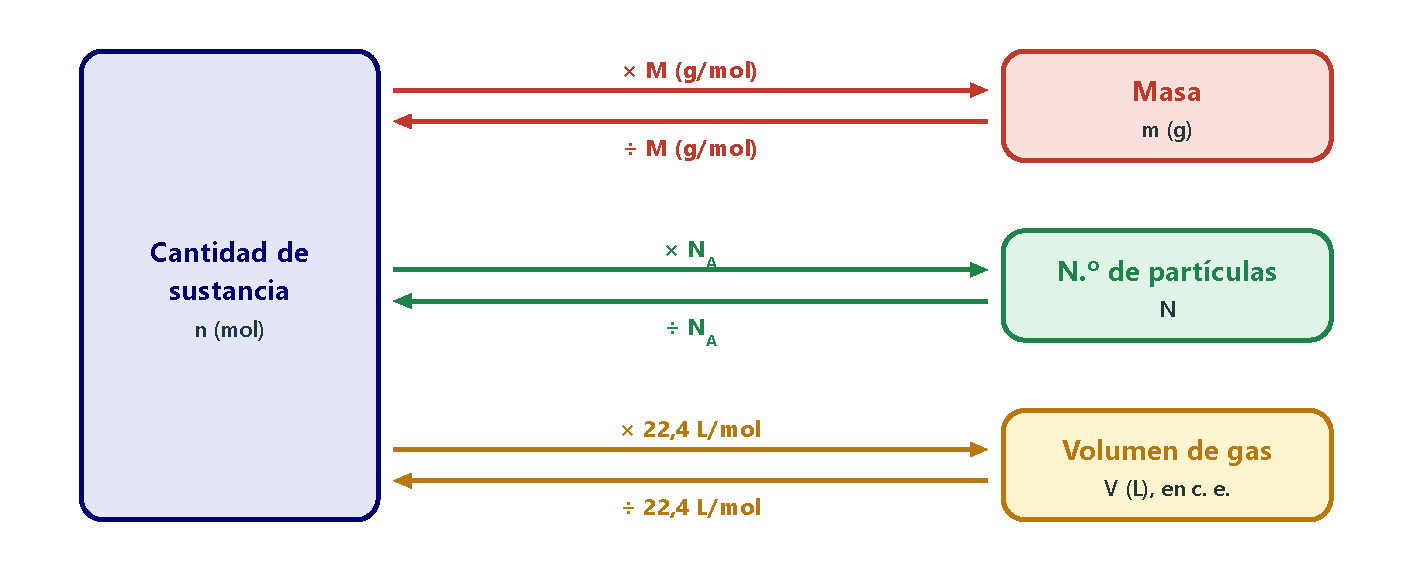
\includegraphics[width=0.85\textwidth]{images/UD5/mol_gas}
    \caption{Relación de la cantidad de sustancia con la masa, el número de partículas y el volumen de un gas en condiciones estándar.}
    \label{fig:mol_gas}
\end{figure}

\begin{example}
    \textbf{¿A qué temperatura están 4 mol de un gas que ocupan \qty{25}{\L} a \qty{4}{\atm}?}
    \[ T = \frac{p V}{n R} = \frac{4 \cdot 25}{4 \cdot \num{0.082}} = \textcolor{red}{\qty{305}{\kelvin}} \]
    \textbf{¿Cuántas moléculas hay en \qty{1}{\cubic\metre} de un gas en condiciones estándar?} \(\qty{1}{\cubic\metre} = \qty{1000}{\L}\):
    \[ n = \frac{\qty{1000}{\L}}{\qty{22.4}{\L\per\mol}} = \qty{44.6}{\mol}; \qquad N = \num{44.6} \cdot \num{6.022e23} = \textcolor{red}{\num{2.69e25}} \text{ moléculas} \]
\end{example}

\begin{exercise}
    ¿Qué volumen ocupan \qty{3}{\mol} de un gas en condiciones estándar?
    \begin{solu}
        \(V = 3 \cdot \num{22.4} = \textcolor{red}{\qty{67.2}{\L}}\).
    \end{solu}
\end{exercise}

\begin{exercise}
    ¿Qué volumen ocupan \num{1.2044e23} moléculas de metano en condiciones estándar?
    \begin{solu}
        \(n = \dfrac{\num{1.2044e23}}{\num{6.022e23}} = \qty{0.2}{\mol}\); \(V = \num{0.2} \cdot \num{22.4} = \textcolor{red}{\qty{4.48}{\L}}\).
    \end{solu}
\end{exercise}

\begin{exercise}
    Completa las frases:
    \begin{enumerate}[label=\alph*)]
        \item El mol, unidad de \ldots, es la cantidad de cualquier conjunto de partículas idénticas que contiene \ldots{} partículas.
        \item Un mol de oxígeno, \ch{O2}, tiene una masa de \ldots{} y ocupa \ldots{} litros en condiciones estándar.
    \end{enumerate}
    \begin{solu}
        a) El mol, unidad de \textcolor{red}{cantidad de sustancia}, contiene \textcolor{red}{\num{6.022e23}} partículas. b) Tiene una masa de \textcolor{red}{\qty{32}{\gram}} y ocupa \textcolor{red}{\qty{22.4}{\L}}.
    \end{solu}
\end{exercise}

\begin{exercise}
    ¿Dónde hay más moléculas: en \qty{5}{\mol} de hidrógeno, \ch{H2}, o en \qty{5}{\mol} de dióxido de carbono, \ch{CO2}? ¿Y más masa?
    \begin{solu}
        Hay el \textcolor{red}{mismo número de moléculas}: \(5 \cdot \num{6.022e23} = \num{3.011e24}\). Tiene más masa el \ch{CO2}: \(5 \cdot 44 = \qty{220}{\gram}\) frente a \(5 \cdot 2 = \qty{10}{\gram}\) de \ch{H2}.
    \end{solu}
\end{exercise}

\begin{exercise}
    Indica si son verdaderas o falsas y corrige las falsas:
    \begin{enumerate}[label=\alph*)]
        \item La ley general de los gases dice que \(p \cdot V / T\) = constante.
        \item El volumen molar es el que ocupa un gas en condiciones estándar.
        \item Un mol de cualquier gas ocupa el mismo volumen que un mol de otro gas si ambos están a la misma presión y temperatura.
        \item \qty{2}{\gram} de hidrógeno ocupan el mismo volumen que \qty{28}{\gram} de nitrógeno aunque no estén en las mismas condiciones.
    \end{enumerate}
    \begin{solu}
        a) \textcolor{red}{Falsa}: la ley general es \(p \cdot V = n \cdot R \cdot T\) (\(pV/T\) = constante es la ley combinada, para una cantidad fija de gas). b) \textcolor{red}{Falsa}: es el volumen que ocupa \emph{un mol} de cualquier gas. c) \textcolor{red}{Verdadera}. d) \textcolor{red}{Falsa}: son \qty{1}{\mol} de cada gas y ocupan el mismo volumen solo si están \emph{en las mismas condiciones}.
    \end{solu}
\end{exercise}

\begin{exercise}
    ¿Cuántas moléculas de nitrógeno hay en \qty{33.6}{\L} de este gas medidos en condiciones estándar?
    \begin{solu}
        \(n = \dfrac{\num{33.6}}{\num{22.4}} = \qty{1.5}{\mol}\); \(N = \num{1.5} \cdot \num{6.022e23} = \textcolor{red}{\num{9.033e23}}\) moléculas.
    \end{solu}
\end{exercise}

\begin{exercise}
    Dos moles de un gas están en un recipiente de \qty{50}{\L} a \qty{27}{\celsius}. a) ¿A qué presión está el gas? b) ¿Cuántas moléculas hay?
    \begin{solu}
        a) \(p = \dfrac{n R T}{V} = \dfrac{2 \cdot \num{0.082} \cdot 300}{50} = \textcolor{red}{\qty{0.98}{\atm}}\). b) \(N = 2 \cdot \num{6.022e23} = \textcolor{red}{\num{1.2044e24}}\) moléculas.
    \end{solu}
\end{exercise}

\begin{exercise}
    Calcula la presión de \qty{0.5}{\mol} de un gas encerrado en un recipiente de \qty{5}{\cubic\deci\metre} a \qty{37}{\celsius}, y el número de moléculas que contiene.
    \begin{solu}
        \(p = \dfrac{\num{0.5} \cdot \num{0.082} \cdot 310}{5} = \textcolor{red}{\qty{2.54}{\atm}}\); \(N = \num{0.5} \cdot \num{6.022e23} = \textcolor{red}{\num{3.011e23}}\) moléculas.
    \end{solu}
\end{exercise}

%========================================================================================
\section{Los sistemas materiales}
%========================================================================================

\begin{definition}[Sistema material]
    Un \textbf{sistema material} es una porción de materia que se separa del resto para estudiarla.
\end{definition}

Según su aspecto, los sistemas materiales se clasifican en (figura~\ref{fig:clasificacion_materia}):
\begin{itemize}
    \item \textbf{Heterogéneos}: no tienen un aspecto uniforme; a simple vista (o con un microscopio) se distinguen sus componentes. Los componentes pueden estar en cualquier proporción y cada uno conserva sus propiedades. Ejemplos: agua y aceite, granito, arena de playa.
    \item \textbf{Homogéneos}: tienen un aspecto uniforme en todos sus puntos. Ejemplos: agua con sal disuelta, agua destilada, aire.
\end{itemize}

\begin{figure}[H]
    \centering
    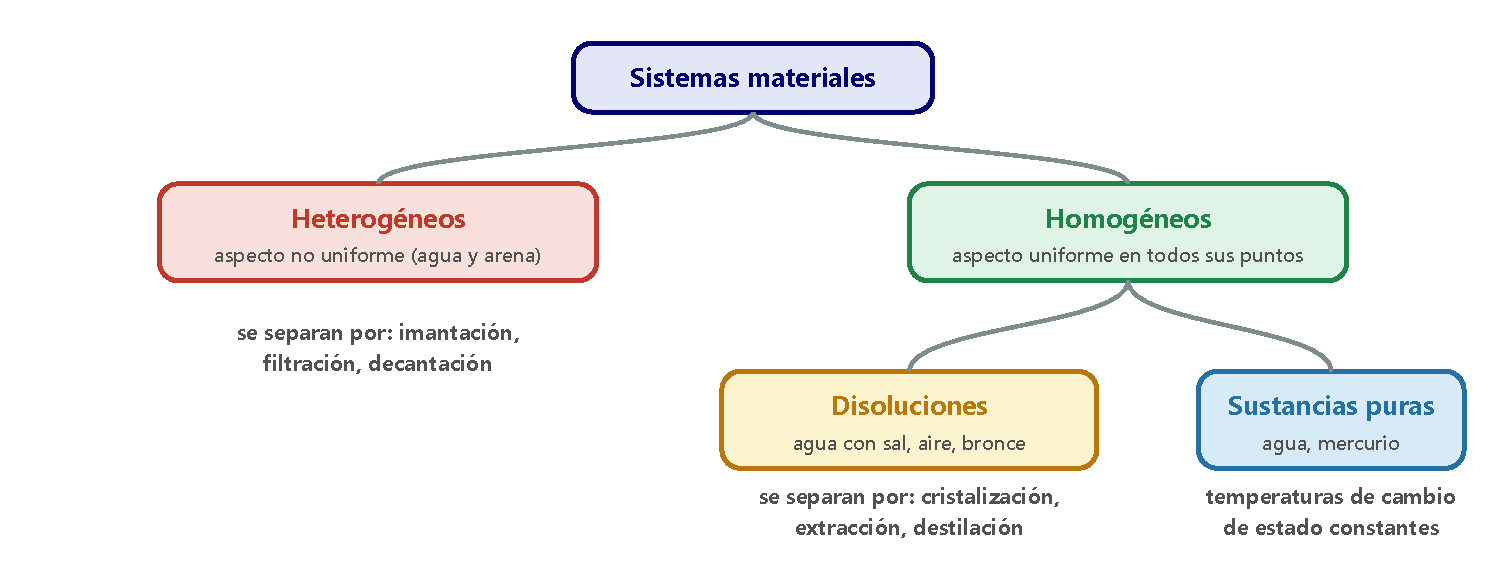
\includegraphics[width=0.95\textwidth]{images/UD5/clasificacion_materia}
    \caption{Clasificación de los sistemas materiales.}
    \label{fig:clasificacion_materia}
\end{figure}

\subsection{¿Cómo se separan los componentes de un sistema heterogéneo?}

Como cada componente conserva sus propiedades, podemos aprovecharlas para separarlos (figura~\ref{fig:separacion_heterogeneos}):
\begin{itemize}
    \item \textbf{Separación magnética.} Separa un sólido magnético (como las limaduras de hierro) de otros que no lo son (arena, sal) acercando un imán.
    \item \textbf{Filtración.} Separa un sólido insoluble de un líquido, por ejemplo arena y agua. Se dobla un papel de filtro, se coloca en un embudo sin que sobresalga y se vierte la mezcla poco a poco ayudándose de una varilla de vidrio. El líquido atraviesa el filtro y el sólido queda retenido.
    \item \textbf{Decantación.} Separa dos líquidos \textbf{inmiscibles} (que no se mezclan) de distinta densidad, como agua y aceite. Se vierte la mezcla en un embudo de decantación y se deja reposar hasta que se formen dos capas. Al abrir la llave sale primero el líquido más denso; cuando ha salido todo, se cierra.
\end{itemize}

\begin{figure}[H]
    \centering
    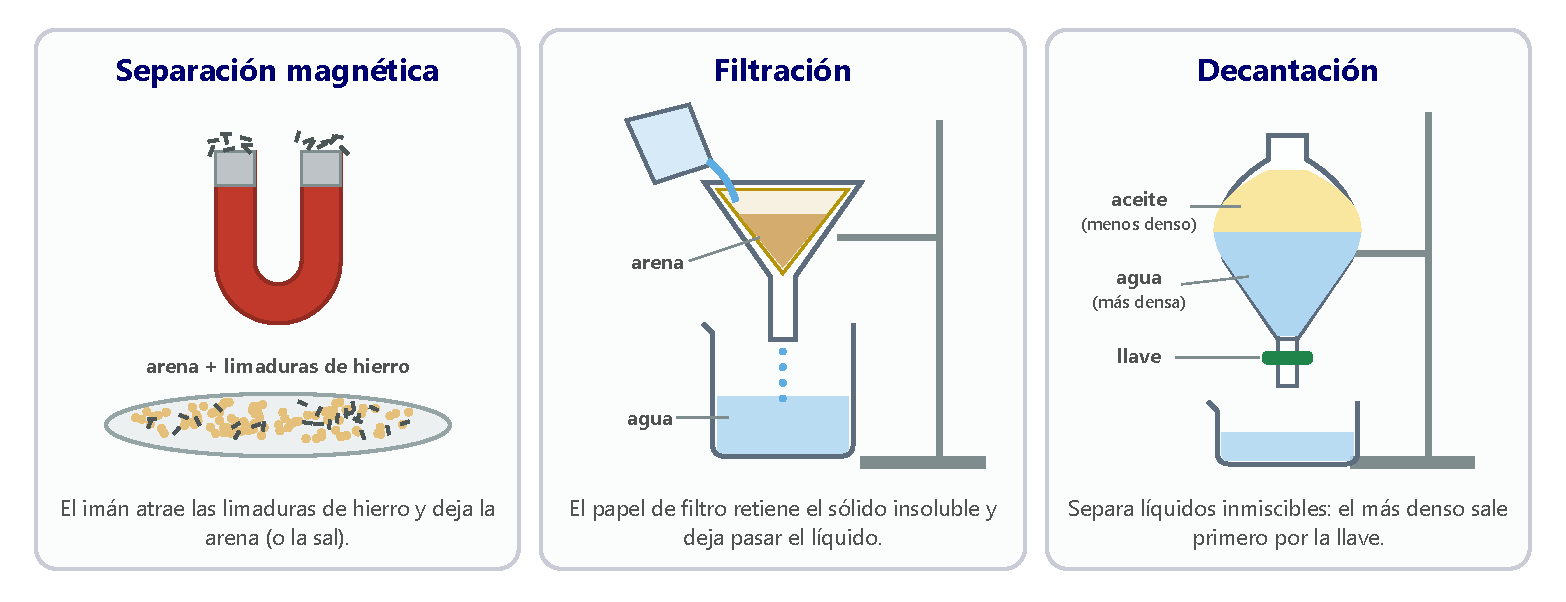
\includegraphics[width=\textwidth]{images/UD5/separacion_heterogeneos}
    \caption{Técnicas para separar los componentes de un sistema heterogéneo.}
    \label{fig:separacion_heterogeneos}
\end{figure}

\begin{exercise}
    Clasifica estos sistemas materiales en homogéneos y heterogéneos: a) agua del grifo; b) agua y arena; c) aceite y vinagre; d) granito; e) aire filtrado; f) vidrio transparente; g) sal común; h) zumo de naranja natural.
    \begin{solu}
        Homogéneos: \textcolor{red}{a), e), f) y g)}. Heterogéneos: \textcolor{red}{b), c), d) y h)} (en el zumo natural se ven la pulpa y otras partículas).
    \end{solu}
\end{exercise}

\begin{exercise}
    ¿Cómo separarías los componentes de estas mezclas?
    \begin{enumerate}[label=\alph*)]
        \item sal y limaduras de hierro;
        \item agua y arena;
        \item limaduras de hierro, arena y agua;
        \item agua y aceite.
    \end{enumerate}
    \begin{solu}
        a) \textcolor{red}{Separación magnética}: el imán atrae el hierro. b) \textcolor{red}{Filtración}: la arena es insoluble en agua. c) Primero \textcolor{red}{filtración} (se separa el agua) y después \textcolor{red}{separación magnética} del hierro y la arena. d) \textcolor{red}{Decantación}: son inmiscibles y tienen distinta densidad.
    \end{solu}
\end{exercise}

\begin{exercise}
    El tetracloruro de carbono es un líquido incoloro, más denso que el agua e inmiscible con ella. ¿Cómo separarías una mezcla de ambos líquidos? ¿Cuál saldrá primero?
    \begin{solu}
        Con un \textcolor{red}{embudo de decantación}, porque son inmiscibles y tienen distinta densidad. Saldrá primero el \textcolor{red}{tetracloruro de carbono}, que es el más denso y queda en la capa inferior.
    \end{solu}
\end{exercise}

%========================================================================================
\section{Sistemas homogéneos: sustancias puras y disoluciones}
%========================================================================================

¿Un sistema homogéneo está formado por una sola sustancia o por varias? Para saberlo se miden sus propiedades características (densidad, temperatura de fusión o de ebullición) y se comprueba si permanecen constantes. Por ejemplo:
\begin{itemize}
    \item El agua con sal empieza a hervir a unos \qty{102}{\celsius}, y su temperatura sigue subiendo mientras hierve.
    \item El agua destilada hierve a \qty{100}{\celsius} y su temperatura no cambia mientras hierve. Lo mismo le pasa al mercurio, pero a \qty{356.7}{\celsius}.
\end{itemize}
El agua destilada y el mercurio son \textbf{sustancias puras}; el agua con sal es una \textbf{disolución}.

\begin{definition}[Sustancia pura y disolución]
    Una \textbf{sustancia pura} tiene una composición fija y unas propiedades características constantes. Una \textbf{disolución} es un sistema material \textbf{homogéneo} y uniforme formado por dos o más sustancias puras en proporción \textbf{variable}.
\end{definition}

\emph{Uniforme} quiere decir que todas las partes de la disolución tienen la misma composición. \emph{Homogéneo} quiere decir que las partículas de los componentes son de tamaño molecular y están repartidas sin ningún orden. En una disolución, las partículas del componente mayoritario, el \textbf{disolvente}, separan y dispersan a las del \textbf{soluto} (figura~\ref{fig:disolucion_particulas}). Así, si dejamos un cristal azul de sulfato de cobre(II) en el fondo de un vaso de agua, poco a poco todo el líquido se vuelve azul: las moléculas de agua chocan con las partículas del cristal y las reparten por todo el vaso.

\begin{figure}[H]
    \centering
    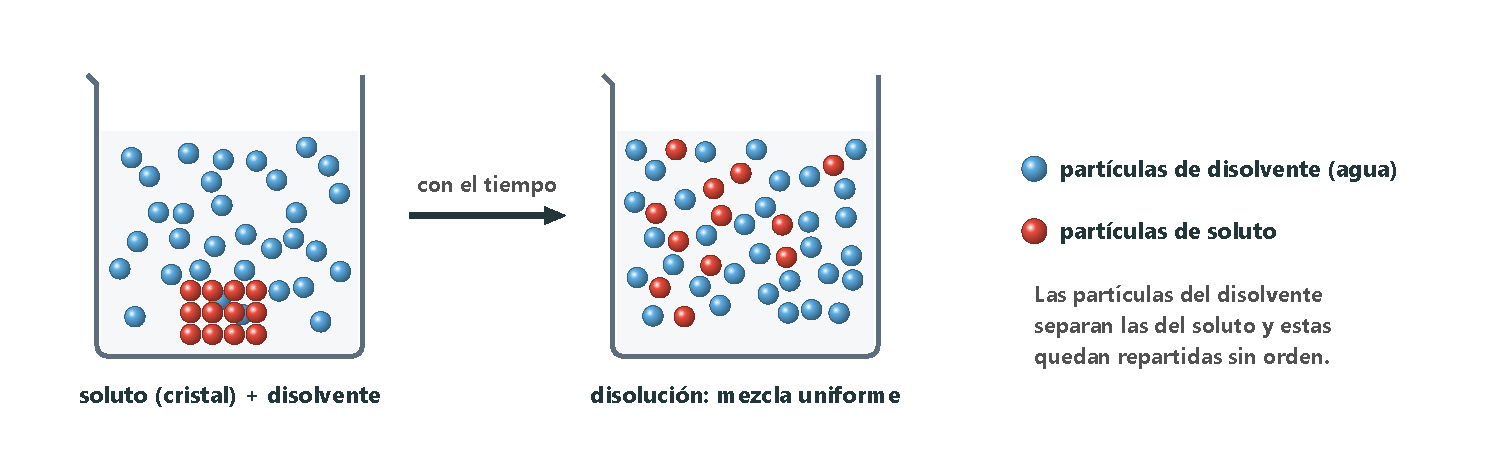
\includegraphics[width=\textwidth]{images/UD5/disolucion_particulas}
    \caption{Al disolverse, las partículas del soluto se reparten entre las del disolvente.}
    \label{fig:disolucion_particulas}
\end{figure}

\begin{exercise}
    Calentamos por separado hasta la ebullición dos líquidos incoloros y transparentes, A y B. Observamos que:
    \begin{enumerate}[label=\arabic*.]
        \item La temperatura de A no cambia mientras hierve y, cuando se evapora todo, no queda nada en el recipiente.
        \item La temperatura de B va subiendo mientras hierve y, cuando se evapora el líquido, queda un residuo blanco.
    \end{enumerate}
    ¿Son sustancias puras o disoluciones?
    \begin{solu}
        A es una \textcolor{red}{sustancia pura}: su temperatura de ebullición es constante y no deja residuo. B es una \textcolor{red}{disolución}: su temperatura de ebullición varía y, al evaporarse el disolvente, queda el soluto sólido.
    \end{solu}
\end{exercise}

\subsection{¿Cómo se expresa la concentración de una disolución?}

\begin{definition}[Concentración]
    La \textbf{concentración} de una disolución es la cantidad de soluto disuelta en una cantidad determinada de disolvente o de disolución.
\end{definition}

\paragraph{Tanto por ciento en masa.} Es la masa de soluto, en gramos, que hay en \qty{100}{\gram} de disolución:
\[ \%\,\text{en masa} = \frac{m_\text{soluto}}{m_\text{disolución}} \cdot 100 \]

\begin{example}
    El oro de 18 quilates es una aleación con un \qty{75}{\percent} en masa de oro; el resto es plata y cobre. ¿Cuánto oro hay en un anillo de \qty{8}{\gram}?
    \[ m_\text{oro} = \frac{75}{100} \cdot \qty{8}{\gram} = \textcolor{red}{\qty{6}{\gram}}; \qquad m_\text{otros metales} = \qty{8}{\gram} - \qty{6}{\gram} = \textcolor{red}{\qty{2}{\gram}} \]
\end{example}

\paragraph{Tanto por ciento en volumen.} Se usa cuando el soluto y el disolvente son líquidos (o gases). Es el volumen de soluto que hay en \qty{100}{\mL} de disolución:
\[ \%\,\text{en volumen} = \frac{V_\text{soluto}}{V_\text{disolución}} \cdot 100 \]

\begin{example}
    ¿Cuánto alcohol hay en un frasco de \qty{250}{\cubic\centi\metre} de alcohol sanitario al \qty{96}{\percent} en volumen?
    \[ V_\text{alcohol} = \frac{96}{100} \cdot \qty{250}{\cubic\centi\metre} = \textcolor{red}{\qty{240}{\cubic\centi\metre}} \]
\end{example}

\paragraph{Concentración en masa.} Es la masa de soluto que hay en cada unidad de volumen de disolución. En el SI se mide en \unit{\kg\per\cubic\metre}, pero lo más habitual es expresarla en \unit{\gram\per\L}:
\[ c = \frac{m_\text{soluto}\,(\unit{\gram})}{V_\text{disolución}\,(\unit{\L})} \]
Por ejemplo, si disolvemos \qty{20}{\gram} de azúcar en agua hasta tener \qty{250}{\mL} de disolución, \(c = \dfrac{\qty{20}{\gram}}{\qty{0.250}{\L}} = \qty{80}{\gram\per\L}\).

\paragraph{Molaridad.}

\begin{definition}[Molaridad, \(M\)]
    La \textbf{molaridad} es la cantidad de soluto, en mol, que hay en un litro de disolución. Se expresa en \unit{\mol\per\L}, unidad que se abrevia como M («molar»):
    \[ M = \frac{n_\text{soluto}\,(\unit{\mol})}{V_\text{disolución}\,(\unit{\L})} \]
\end{definition}

\begin{example}
    Calcula la molaridad de una disolución preparada disolviendo \qty{5.85}{\gram} de cloruro de sodio, \ch{NaCl}, en agua hasta tener \qty{200}{\mL} de disolución (\(A_r\): Na = 23; Cl = \num{35.5}).

    \textcolor{blue}{Masa molar:} \(M(\ch{NaCl}) = \qty{58.5}{\gram\per\mol}\). \quad \textcolor{blue}{Cantidad de soluto:} \(n = \dfrac{\num{5.85}}{\num{58.5}} = \qty{0.1}{\mol}\).
    \[ M = \frac{\qty{0.1}{\mol}}{\qty{0.200}{\L}} = \textcolor{red}{\qty{0.5}{\mol\per\L}} \;(\num{0.5}\,\text{M}) \]
\end{example}

\begin{exercise}
    El acero inoxidable de algunos cuchillos tiene un \qty{0.3}{\percent} de carbono, un \qty{18}{\percent} de cromo y un \qty{8}{\percent} de níquel (el resto es hierro). ¿Qué masa de cada elemento hay en una hoja de \qty{200}{\gram}?
    \begin{solu}
        C: \(\frac{\num{0.3}}{100} \cdot 200 = \textcolor{red}{\qty{0.6}{\gram}}\); Cr: \(\frac{18}{100} \cdot 200 = \textcolor{red}{\qty{36}{\gram}}\); Ni: \(\frac{8}{100} \cdot 200 = \textcolor{red}{\qty{16}{\gram}}\); Fe: \(200 - \num{52.6} = \textcolor{red}{\qty{147.4}{\gram}}\).
    \end{solu}
\end{exercise}

\begin{exercise}
    Un joyero funde \qty{15}{\gram} de oro con \qty{5}{\gram} de plata. ¿Cuál es el tanto por ciento en masa de cada metal en la aleación?
    \begin{solu}
        \(m_\text{aleación} = 15 + 5 = \qty{20}{\gram}\). \(\%\,\text{oro} = \frac{15}{20} \cdot 100 = \textcolor{red}{\qty{75}{\percent}}\); \(\%\,\text{plata} = \frac{5}{20} \cdot 100 = \textcolor{red}{\qty{25}{\percent}}\).
    \end{solu}
\end{exercise}

\begin{exercise}
    ¿Qué volumen de un líquido debes usar para preparar \qty{500}{\cubic\centi\metre} de una disolución acuosa al \qty{70}{\percent} en volumen?
    \begin{solu}
        \(V = \frac{70}{100} \cdot 500 = \textcolor{red}{\qty{350}{\cubic\centi\metre}}\), completando con agua hasta \qty{500}{\cubic\centi\metre}.
    \end{solu}
\end{exercise}

\begin{exercise}
    Calcula la molaridad de una disolución que contiene \qty{12}{\gram} de hidróxido de sodio, \ch{NaOH}, en \qty{1}{\L} de disolución (\(A_r\): Na = 23; O = 16; H = 1).
    \begin{solu}
        \(M(\ch{NaOH}) = \qty{40}{\gram\per\mol}\); \(n = \frac{12}{40} = \qty{0.3}{\mol}\); \(M = \frac{\num{0.3}}{1} = \textcolor{red}{\qty{0.3}{\mol\per\L}}\).
    \end{solu}
\end{exercise}

\begin{exercise}
    ¿Qué masa de \ch{NaOH} hay que disolver para preparar \qty{250}{\mL} de disolución \num{0.2} M?
    \begin{solu}
        \(n = M \cdot V = \num{0.2} \cdot \num{0.250} = \qty{0.05}{\mol}\); \(m = \num{0.05} \cdot 40 = \textcolor{red}{\qty{2}{\gram}}\).
    \end{solu}
\end{exercise}

\begin{exercise}
    Se disuelven \qty{20}{\gram} de bromuro de potasio, \ch{KBr}, en agua hasta tener \qty{400}{\mL} de disolución. Calcula su molaridad (\(A_r\): K = 39; Br = 80).
    \begin{solu}
        \(M(\ch{KBr}) = \qty{119}{\gram\per\mol}\); \(n = \frac{20}{119} = \qty{0.168}{\mol}\); \(M = \frac{\num{0.168}}{\num{0.400}} = \textcolor{red}{\qty{0.42}{\mol\per\L}}\).
    \end{solu}
\end{exercise}

\begin{exercise}
    Se prepara una disolución con \qty{1}{\gram} de cloruro de potasio y \qty{2}{\gram} de cloruro de sodio en \qty{500}{\gram} de agua. ¿Cuál es el tanto por ciento en masa de cada componente?
    \begin{solu}
        \(m_\text{disolución} = 1 + 2 + 500 = \qty{503}{\gram}\).
        \(\%\,\ch{KCl} = \frac{1}{503} \cdot 100 = \textcolor{red}{\qty{0.199}{\percent}}\); \(\%\,\ch{NaCl} = \frac{2}{503} \cdot 100 = \textcolor{red}{\qty{0.398}{\percent}}\); \(\%\,\text{agua} = \frac{500}{503} \cdot 100 = \textcolor{red}{\qty{99.40}{\percent}}\).
    \end{solu}
\end{exercise}

\begin{exercise}
    Para fabricar una joya de \qty{12}{\gram}, un joyero usa una aleación con un \qty{80}{\percent} de oro y un \qty{20}{\percent} de níquel. ¿Qué masa de cada metal necesita?
    \begin{solu}
        Oro: \(\frac{80}{100} \cdot 12 = \textcolor{red}{\qty{9.6}{\gram}}\); níquel: \(\frac{20}{100} \cdot 12 = \textcolor{red}{\qty{2.4}{\gram}}\).
    \end{solu}
\end{exercise}

\begin{exercise}
    Un bronce contiene un \qty{90}{\percent} de cobre y un \qty{10}{\percent} de estaño. ¿Qué masa de cada metal hay que fundir para fabricar una campana de \qty{25}{\kg}?
    \begin{solu}
        Cobre: \(\frac{90}{100} \cdot 25 = \textcolor{red}{\qty{22.5}{\kg}}\); estaño: \(\frac{10}{100} \cdot 25 = \textcolor{red}{\qty{2.5}{\kg}}\).
    \end{solu}
\end{exercise}

\begin{exercise}
    Un latón tiene un \qty{65}{\percent} de cobre y un \qty{35}{\percent} de zinc. ¿Qué masa de cada metal hace falta para una plancha de latón de \qty{40}{\kg}?
    \begin{solu}
        Cobre: \(\frac{65}{100} \cdot 40 = \textcolor{red}{\qty{26}{\kg}}\); zinc: \(\frac{35}{100} \cdot 40 = \textcolor{red}{\qty{14}{\kg}}\).
    \end{solu}
\end{exercise}

\begin{exercise}
    En el envase de un colutorio de \qty{250}{\mL} pone: «Composición: \qty{0.12}{\percent} de digluconato de clorhexidina y \qty{2}{\percent} de xilitol» (gramos por cada \qty{100}{\mL}).
    \begin{enumerate}[label=\alph*)]
        \item ¿Qué cantidad de cada sustancia hay en el frasco?
        \item Cada enjuague se hace con \qty{15}{\mL}. ¿Qué cantidad de cada componente se usa en un enjuague?
    \end{enumerate}
    \begin{solu}
        a) Clorhexidina: \(\frac{\num{0.12}}{100} \cdot 250 = \textcolor{red}{\qty{0.3}{\gram}}\); xilitol: \(\frac{2}{100} \cdot 250 = \textcolor{red}{\qty{5}{\gram}}\).
        b) Clorhexidina: \(\frac{\num{0.12}}{100} \cdot 15 = \textcolor{red}{\qty{0.018}{\gram}}\); xilitol: \(\frac{2}{100} \cdot 15 = \textcolor{red}{\qty{0.3}{\gram}}\).
    \end{solu}
\end{exercise}

\begin{exercise}
    El prospecto de un jarabe dice: «Solución oral: \qty{150}{\mL}. Composición: \qty{4}{\milli\gram\per\mL} de principio activo. Tomar \qty{5}{\mL} cada ocho horas».
    \begin{enumerate}[label=\alph*)]
        \item ¿Cuánto principio activo hay en el frasco?
        \item ¿Cuánto se toma en cada dosis?
        \item ¿Y en un día?
    \end{enumerate}
    \begin{solu}
        a) \(4 \cdot 150 = \textcolor{red}{\qty{600}{\milli\gram}}\). b) \(4 \cdot 5 = \textcolor{red}{\qty{20}{\milli\gram}}\). c) Tres dosis: \(\textcolor{red}{\qty{60}{\milli\gram}}\).
    \end{solu}
\end{exercise}

\begin{exercise}
    Una disolución de \ch{HCl} contiene \qty{7.3}{\gram} de soluto en \qty{250}{\cubic\centi\metre} de disolución. Calcula su molaridad (\(A_r\): Cl = \num{35.5}; H = 1).
    \begin{solu}
        \(M(\ch{HCl}) = \qty{36.5}{\gram\per\mol}\); \(n = \frac{\num{7.3}}{\num{36.5}} = \qty{0.2}{\mol}\); \(M = \frac{\num{0.2}}{\num{0.250}} = \textcolor{red}{\qty{0.8}{\mol\per\L}}\).
    \end{solu}
\end{exercise}

\begin{exercise}
    Se disuelven \qty{17.1}{\gram} de sacarosa (azúcar, \(M = \qty{342}{\gram\per\mol}\)) en agua hasta \qty{500}{\mL} de disolución. ¿Cuál es su molaridad?
    \begin{solu}
        \(n = \frac{\num{17.1}}{342} = \qty{0.05}{\mol}\); \(M = \frac{\num{0.05}}{\num{0.500}} = \textcolor{red}{\qty{0.1}{\mol\per\L}}\).
    \end{solu}
\end{exercise}

\begin{exercise}
    Una disolución contiene \qty{49}{\gram} de ácido sulfúrico, \ch{H2SO4}, en \qty{2}{\L}. ¿Cuál es su molaridad? (\(A_r\): S = 32).
    \begin{solu}
        \(M(\ch{H2SO4}) = 2 + 32 + 64 = \qty{98}{\gram\per\mol}\); \(n = \frac{49}{98} = \qty{0.5}{\mol}\); \(M = \frac{\num{0.5}}{2} = \textcolor{red}{\qty{0.25}{\mol\per\L}}\).
    \end{solu}
\end{exercise}

\begin{exercise}
    Calcula la molaridad de una disolución preparada disolviendo \qty{29.25}{\gram} de \ch{NaCl} en agua hasta tener \qty{250}{\mL} de disolución.
    \begin{solu}
        \(n = \frac{\num{29.25}}{\num{58.5}} = \qty{0.5}{\mol}\); \(M = \frac{\num{0.5}}{\num{0.250}} = \textcolor{red}{\qty{2}{\mol\per\L}}\).
    \end{solu}
\end{exercise}

\begin{exercise}
    Asigna a cada frasco su etiqueta: \num{0.1} M, \num{0.5} M, 1 M o 2 M.
    \begin{enumerate}[label=\alph*)]
        \item \qty{20}{\gram} de \ch{NaOH} en \qty{1}{\L};
        \item \qty{80}{\gram} de \ch{NaOH} en \qty{1}{\L};
        \item \qty{4}{\gram} de \ch{NaOH} en \qty{100}{\mL};
        \item \qty{0.4}{\gram} de \ch{NaOH} en \qty{100}{\mL}.
    \end{enumerate}
    \begin{solu}
        \textcolor{blue}{\(M(\ch{NaOH}) = \qty{40}{\gram\per\mol}\).} a) \(\frac{\num{0.5}}{1}\) \(\Rightarrow\) \textcolor{red}{\num{0.5} M}. b) \(\frac{2}{1}\) \(\Rightarrow\) \textcolor{red}{2 M}. c) \(\frac{\num{0.1}}{\num{0.1}}\) \(\Rightarrow\) \textcolor{red}{1 M}. d) \(\frac{\num{0.01}}{\num{0.1}}\) \(\Rightarrow\) \textcolor{red}{\num{0.1} M}.
    \end{solu}
\end{exercise}

\begin{exercise}
    Indica la molaridad de una disolución que contiene \qty{11.2}{\gram} de hidróxido de potasio, \ch{KOH}, en \qty{2}{\L} de disolución (\(A_r\): K = 39).
    \begin{solu}
        \(M(\ch{KOH}) = \qty{56}{\gram\per\mol}\); \(n = \frac{\num{11.2}}{56} = \qty{0.2}{\mol}\); \(M = \frac{\num{0.2}}{2} = \textcolor{red}{\qty{0.1}{\mol\per\L}}\).
    \end{solu}
\end{exercise}

\subsection{¿Cómo se prepara una disolución de concentración conocida?}

Queremos preparar \qty{250}{\mL} de disolución 1 M de cloruro de sodio. Primero calculamos la masa de soluto:
\[ n = M \cdot V = \qty{1}{\mol\per\L} \cdot \qty{0.250}{\L} = \qty{0.25}{\mol}; \qquad m = n \cdot M(\ch{NaCl}) = \num{0.25} \cdot \num{58.5} = \qty{14.625}{\gram} \]
Después seguimos estos pasos (figura~\ref{fig:preparar_disolucion}):

\begin{enumerate}[label=\numberballgreen]
    \item Pesamos \qty{14.63}{\gram} de \ch{NaCl} en un vaso de precipitados con una balanza digital.
    \item Añadimos unos \qty{100}{\mL} de agua destilada y disolvemos la sal con una varilla de vidrio.
    \item Trasvasamos la disolución a un matraz aforado de \qty{250}{\mL} con ayuda de la varilla y de un embudo. Enjuagamos el vaso con un poco de agua y la echamos también al matraz.
    \item Añadimos agua destilada poco a poco hasta \textbf{enrasar}: la parte baja del menisco debe tocar la marca del aforo.
\end{enumerate}

\begin{figure}[H]
    \centering
    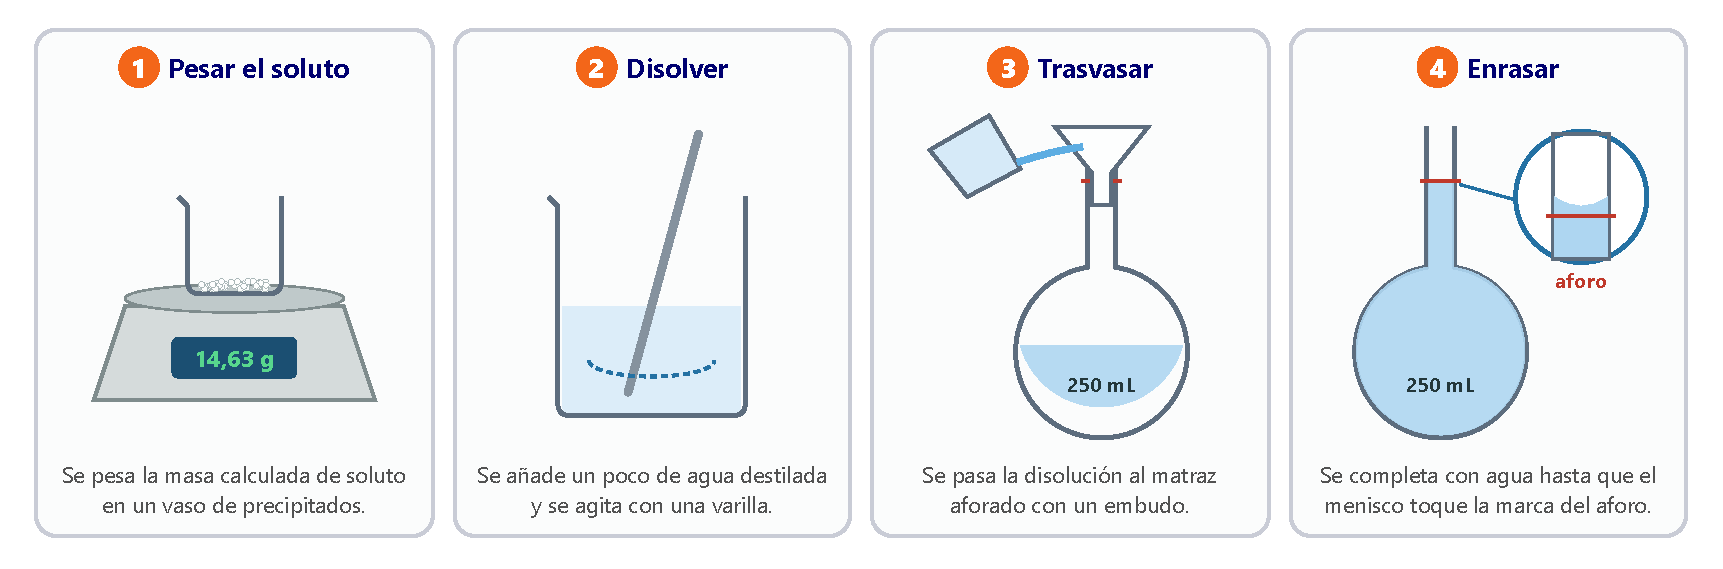
\includegraphics[width=\textwidth]{images/UD5/preparar_disolucion}
    \caption{Pasos para preparar una disolución de concentración conocida.}
    \label{fig:preparar_disolucion}
\end{figure}

\begin{exercise}
    Explica con detalle cómo prepararías \qty{250}{\mL} de disolución \num{0.2} M de cloruro de potasio, \ch{KCl} (\(A_r\): K = 39; Cl = \num{35.5}). ¿Qué material de laboratorio necesitas?
    \begin{solu}
        \textcolor{blue}{Cálculo:} \(n = \num{0.2} \cdot \num{0.250} = \qty{0.05}{\mol}\); \(m = \num{0.05} \cdot \num{74.5} = \textcolor{red}{\qty{3.725}{\gram}}\) de \ch{KCl}.
        \textcolor{blue}{Procedimiento:} se pesan \qty{3.73}{\gram} de \ch{KCl} en un vaso de precipitados con una balanza; se añade un poco de agua destilada y se disuelve con una varilla; se trasvasa a un matraz aforado de \qty{250}{\mL} con un embudo; se añade agua destilada hasta enrasar.
        \textcolor{blue}{Material:} balanza, vaso de precipitados, varilla de vidrio, embudo, matraz aforado de \qty{250}{\mL}, frasco lavador con agua destilada.
    \end{solu}
\end{exercise}

\begin{exercise}
    ¿Qué masa de cloruro de sodio necesitas para preparar \qty{500}{\mL} de disolución acuosa \num{0.2} M?
    \begin{solu}
        \(n = \num{0.2} \cdot \num{0.500} = \qty{0.1}{\mol}\); \(m = \num{0.1} \cdot \num{58.5} = \textcolor{red}{\qty{5.85}{\gram}}\) de \ch{NaCl}, que se disuelven en agua hasta completar \qty{500}{\mL} en un matraz aforado.
    \end{solu}
\end{exercise}

\subsection{¿Cómo se separan los componentes de una disolución?}

\begin{itemize}
    \item \textbf{Cristalización.} Separa un \textbf{soluto sólido} del disolvente; es el proceso inverso a la disolución. Se calienta la disolución para evaporar parte del disolvente, se filtra para eliminar impurezas y se deja enfriar en un cristalizador. Si el enfriamiento es lento, se forman cristales grandes; si es rápido, pequeños.
    \item \textbf{Extracción con disolventes.} Aprovecha que una sustancia es más soluble en un disolvente que en otro. Por ejemplo, el bromo es más soluble en tetracloruro de carbono que en agua. Si añadimos \ch{CCl4} (inmiscible con el agua) a una disolución de bromo en agua y agitamos, el bromo pasa al \ch{CCl4}. Después se separan las dos capas con un embudo de decantación.
    \item \textbf{Destilación simple.} Separa dos líquidos con \textbf{distinta temperatura de ebullición}. Al calentar la disolución en un matraz, el líquido más volátil se evapora antes; su vapor pasa por un \textbf{refrigerante}, por el que circula agua fría, se condensa y se recoge en un vaso o un Erlenmeyer. En el matraz queda el otro componente.
\end{itemize}

\begin{figure}[H]
    \centering
    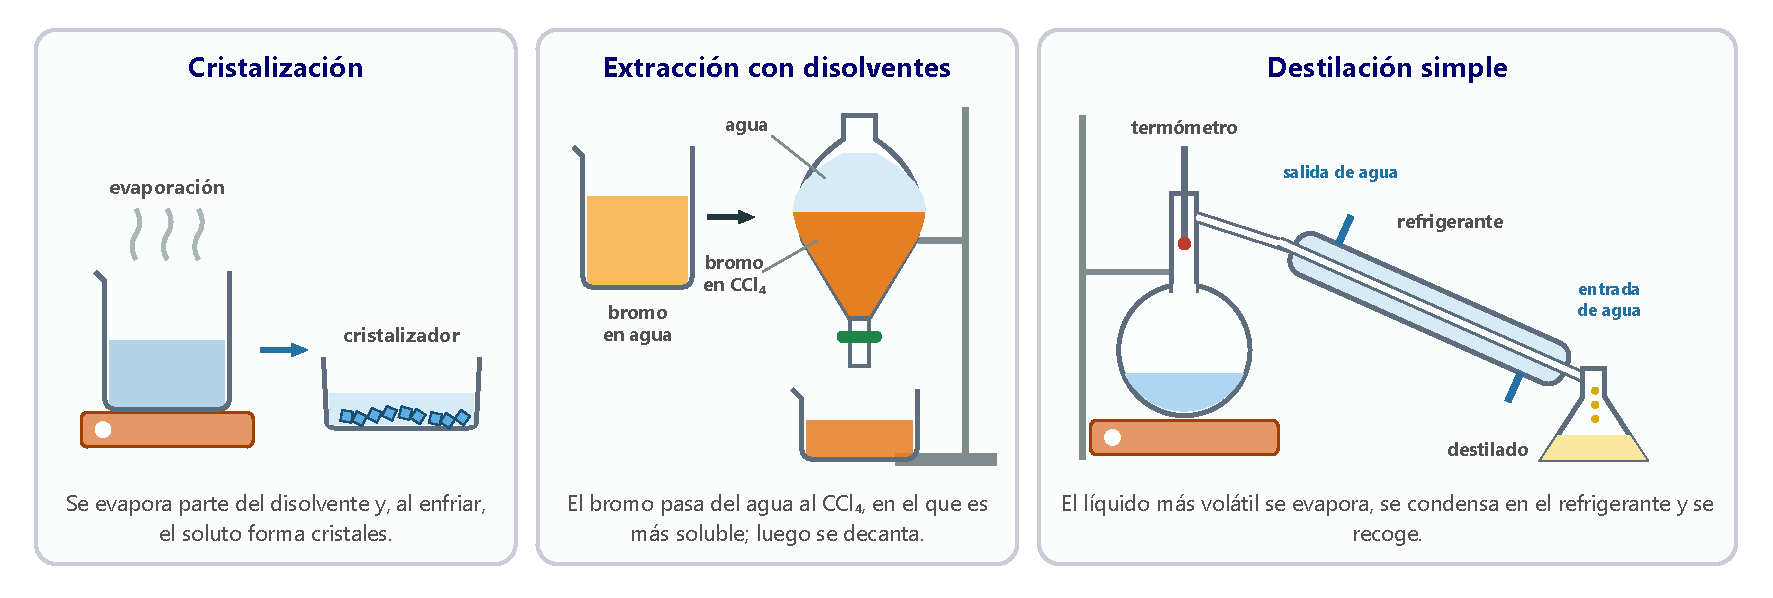
\includegraphics[width=\textwidth]{images/UD5/separacion_disoluciones}
    \caption{Técnicas para separar los componentes de una disolución.}
    \label{fig:separacion_disoluciones}
\end{figure}

\begin{exercise}
    ¿Cuándo se puede usar la extracción con disolventes para separar los componentes de una disolución? Describe el procedimiento.
    \begin{solu}
        Cuando hay un segundo disolvente, \textcolor{red}{inmiscible con el primero}, en el que el soluto es \textcolor{red}{mucho más soluble}. Se añade ese disolvente, se agita para que el soluto pase a él, se deja reposar hasta que se formen dos capas y se separan con un embudo de decantación. Por ejemplo, las grasas son insolubles en agua pero solubles en tolueno.
    \end{solu}
\end{exercise}

\begin{exercise}
    ¿Cuándo se puede usar la cristalización? ¿Sirve para separar los componentes de una disolución en la que el soluto y el disolvente son líquidos?
    \begin{solu}
        Cuando el soluto es un \textcolor{red}{sólido} disuelto en un líquido que se puede evaporar. \textcolor{red}{No} sirve si los dos componentes son líquidos: en ese caso se usa la destilación.
    \end{solu}
\end{exercise}

\begin{exercise}
    ¿Cuándo se puede usar la destilación para separar dos líquidos? ¿Podría usarse para recuperar el agua de una disolución de sal?
    \begin{solu}
        Cuando los dos líquidos tienen \textcolor{red}{distintas temperaturas de ebullición}. \textcolor{red}{Sí}: el agua se evapora, se condensa en el refrigerante y se recoge, y la sal queda en el matraz.
    \end{solu}
\end{exercise}

\begin{exercise}
    ¿En qué técnica (cristalización, extracción con disolventes o destilación) usarías cada uno de estos materiales? Un material puede servir para más de una.
    \begin{enumerate}[label=\alph*)]
        \item placa calefactora;
        \item embudo;
        \item embudo de decantación;
        \item cristalizador;
        \item matraz de destilación;
        \item refrigerante.
    \end{enumerate}
    \begin{solu}
        a) \textcolor{red}{Cristalización y destilación}. b) \textcolor{red}{Cristalización} (para filtrar). c) \textcolor{red}{Extracción}. d) \textcolor{red}{Cristalización}. e) y f) \textcolor{red}{Destilación}.
    \end{solu}
\end{exercise}

\begin{exercise}
    Describe cómo separarías los componentes de: a) una disolución de sulfato de cobre(II) en agua; b) una disolución de yodo en agua; c) una mezcla de alcohol y agua.
    \begin{solu}
        a) \textcolor{red}{Cristalización}: se evapora parte del agua y, al enfriar, cristaliza el sulfato de cobre(II). b) \textcolor{red}{Extracción con disolventes}: se añade un disolvente inmiscible con el agua en el que el yodo es más soluble (por ejemplo, \ch{CCl4}) y después se decanta. c) \textcolor{red}{Destilación simple}: el alcohol hierve a menor temperatura (\qty{78}{\celsius}) que el agua.
    \end{solu}
\end{exercise}


%------------------------------------------------


    \chapterimage{images/portada_cabeceras/cabecera_UD6}
    \chapter{Las reacciones químicas}

    %! Author = crist
%! Date = 25/10/2026

\spacing{1.3}
%----------------------------------------------------------------------------------------
%	UNIDAD 6: LAS REACCIONES QUÍMICAS (4.º ESO)
%   Figuras: images/UD6/*.pdf (fuente HTML en images/UD6/html, SVG en images/UD6/svg)
%----------------------------------------------------------------------------------------

% Mapa conceptual del tema (fuente en images/mapas_conceptuales/html/temas.js)
\begin{figure}[H]
    \centering
    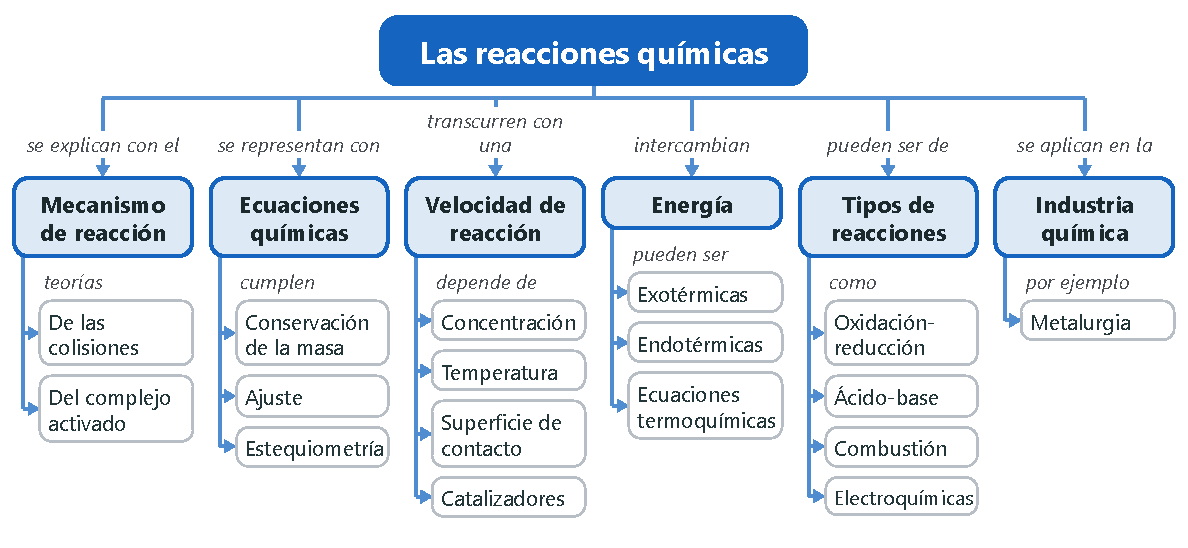
\includegraphics[width=\textwidth]{images/mapas_conceptuales/mapa_UD6}
\end{figure}

%========================================================================================
%\section*{Para empezar: el dióxido de carbono y el efecto invernadero}
%\addcontentsline{toc}{section}{Para empezar: el dióxido de carbono y el efecto invernadero}
%========================================================================================
%
%Antes de la Revolución Industrial, el aire contenía unas 280 partes por millón (ppm) de dióxido de carbono. El \ch{CO2} retiene cerca de la superficie parte del calor que la Tierra emitiría al espacio, y gracias a ese «termostato» la temperatura media del planeta se mantuvo en torno a \qty{14}{\celsius}: con ese clima construimos nuestras ciudades y aprendimos a cultivar.
%
%Cuando empezamos a quemar carbón, petróleo y gas para obtener energía, la cantidad de \ch{CO2} empezó a subir: en 2007 ya era de 380~ppm y en 2022 alcanzó las 420~ppm, el valor más alto desde que hay registros. El \ch{CO2} es un gas \textbf{persistente}: permanece mucho tiempo en la atmósfera y lo que se emite se va acumulando. El calentamiento resultante está fundiendo los hielos, cambiando las estaciones y el régimen de lluvias, y haciendo subir el nivel del mar.
%
%La principal reacción responsable es la \textbf{combustión}: \ch{C + O2 -> CO2}. Reducir sus emisiones está relacionado con los \textbf{ODS 7} (\emph{Energía asequible y no contaminante}), \textbf{11} (\emph{Ciudades y comunidades sostenibles}), \textbf{12} (\emph{Producción y consumo responsables}) y \textbf{13} (\emph{Acción por el clima}). Pero, además de las decisiones de los gobiernos, hará falta la acción de cada persona.
%
%\begin{exercise}
%    ¿Cuánto \ch{CO2} había en la atmósfera antes de la Revolución Industrial? ¿Por qué ha aumentado desde entonces? ¿Qué reacción química es la principal responsable?
%    \begin{solu}
%        Unas \textcolor{red}{280~ppm}. Ha aumentado por la \textcolor{red}{quema de combustibles fósiles} (carbón, petróleo y gas) en la industria, el transporte y la producción de energía. La reacción responsable es la combustión: \ch{C + O2 -> CO2}.
%    \end{solu}
%\end{exercise}
%
%\begin{exercise}
%    ¿Qué concentración de \ch{CO2} se midió en 2007 y en 2022? ¿Qué consecuencias del calentamiento se observaban ya en 2007? ¿Es fácil eliminar el \ch{CO2} acumulado?
%    \begin{solu}
%        \textcolor{red}{380~ppm} en 2007 y \textcolor{red}{420~ppm} en 2022: la situación no ha mejorado. Ya en 2007 se observaban la fusión de los hielos, cambios en las estaciones y en las lluvias y la subida del nivel del mar. No es fácil eliminarlo: es un gas \textcolor{red}{persistente}.
%    \end{solu}
%\end{exercise}
%
%\begin{exercise}
%    ¿Cómo pueden ayudar los ODS 7, 11, 12 y 13 a reducir los gases de efecto invernadero? ¿Qué puedes hacer tú?
%    \begin{solu}
%        Promueven energías limpias, ciudades sostenibles, un consumo responsable y medidas contra el cambio climático, todo lo cual reduce las emisiones. Respuesta libre para la acción individual: usar transporte público o bicicleta, ahorrar energía en casa, consumir productos locales, reciclar\ldots
%    \end{solu}
%\end{exercise}

%========================================================================================
\section{¿Cómo se produce una reacción? El mecanismo de reacción}
%========================================================================================

Si calentamos en una cápsula de porcelana una mezcla de aluminio y yodo, el conjunto arde con grandes llamas y al final queda un polvo blanco: una sustancia nueva, el triyoduro de aluminio:
\[ \ch{2 Al (s) + 3 I2 (s) -> 2 AlI3 (s)} \]
Para que ocurra, se han \textbf{roto} los enlaces metálicos del aluminio y los enlaces covalentes del yodo, y se han \textbf{formado} enlaces nuevos entre el aluminio y el yodo.

\begin{definition}[Reacción química y mecanismo de reacción]
    En una \textbf{reacción química} se rompen enlaces de las sustancias iniciales, los \textbf{reactivos}, y sus átomos se reorganizan formando enlaces nuevos para dar sustancias distintas, los \textbf{productos}. El conjunto de procesos elementales por los que transcurre se llama \textbf{mecanismo de reacción}.
\end{definition}

Dos teorías explican el mecanismo de las reacciones: la teoría de las colisiones y la del complejo activado.

\subsection{La teoría de las colisiones}

Según el modelo cinético de la materia, las partículas están en continuo movimiento. Para que reaccionen, las partículas de los reactivos (átomos, moléculas o iones) tienen que \textbf{chocar}. Pero no todos los choques sirven: un \textbf{choque es eficaz} solo si las partículas chocan
\begin{itemize}
    \item con \textbf{energía suficiente}: si no, se limitan a rebotar;
    \item con la \textbf{orientación adecuada}: aunque choquen con mucha energía, si no se orientan bien no pueden romperse los enlaces para formar los nuevos.
\end{itemize}

\begin{figure}[H]
    \centering
    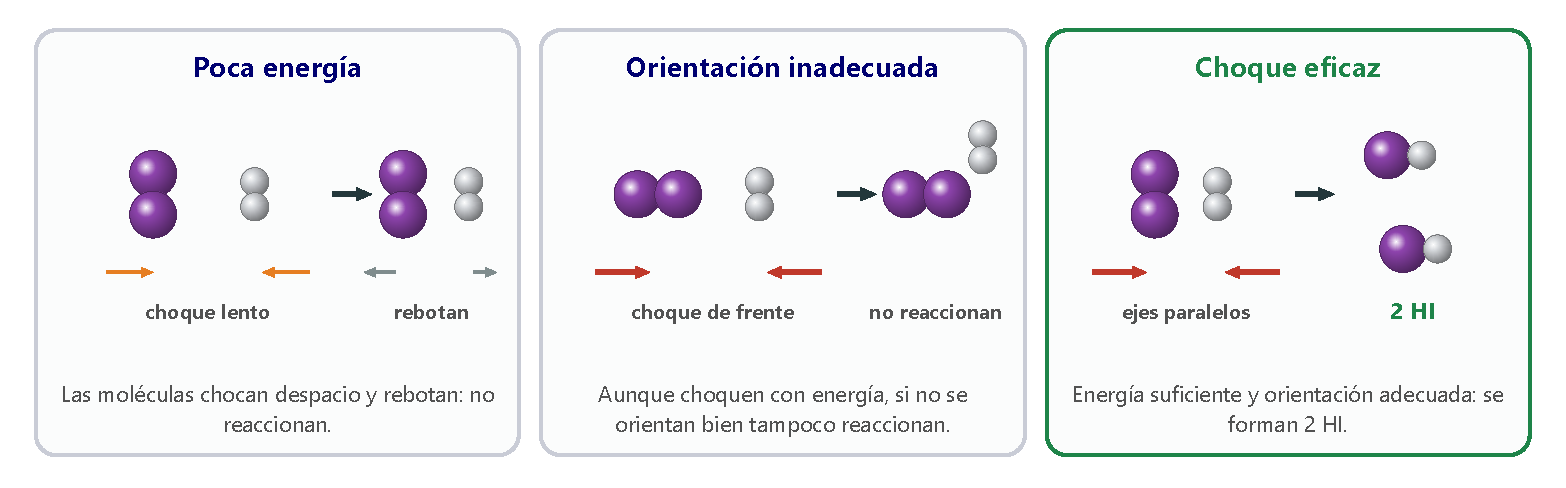
\includegraphics[width=\textwidth]{images/UD6/colisiones}
    \caption{Choques entre moléculas de \ch{I2} (moradas) y de \ch{H2} (grises). Solo el último es eficaz.}
    \label{fig:colisiones}
\end{figure}

\subsection{La teoría del complejo activado}

Cuando las partículas chocan con energía y orientación adecuadas, sus átomos pasan, durante un instante, por una agrupación inestable de alta energía: el \textbf{complejo activado}. En él, los enlaces de los reactivos se han debilitado y los de los productos han empezado a formarse. Desde ahí puede dar los productos o volver a dar los reactivos.

\begin{definition}[Energía de activación, \(E_a\)]
    Es la energía mínima que necesitan las partículas que chocan con la orientación adecuada para formar el complejo activado y que la reacción tenga lugar. En el diagrama de energía es la «barrera» entre los reactivos y el complejo activado.
\end{definition}

\begin{figure}[H]
    \centering
    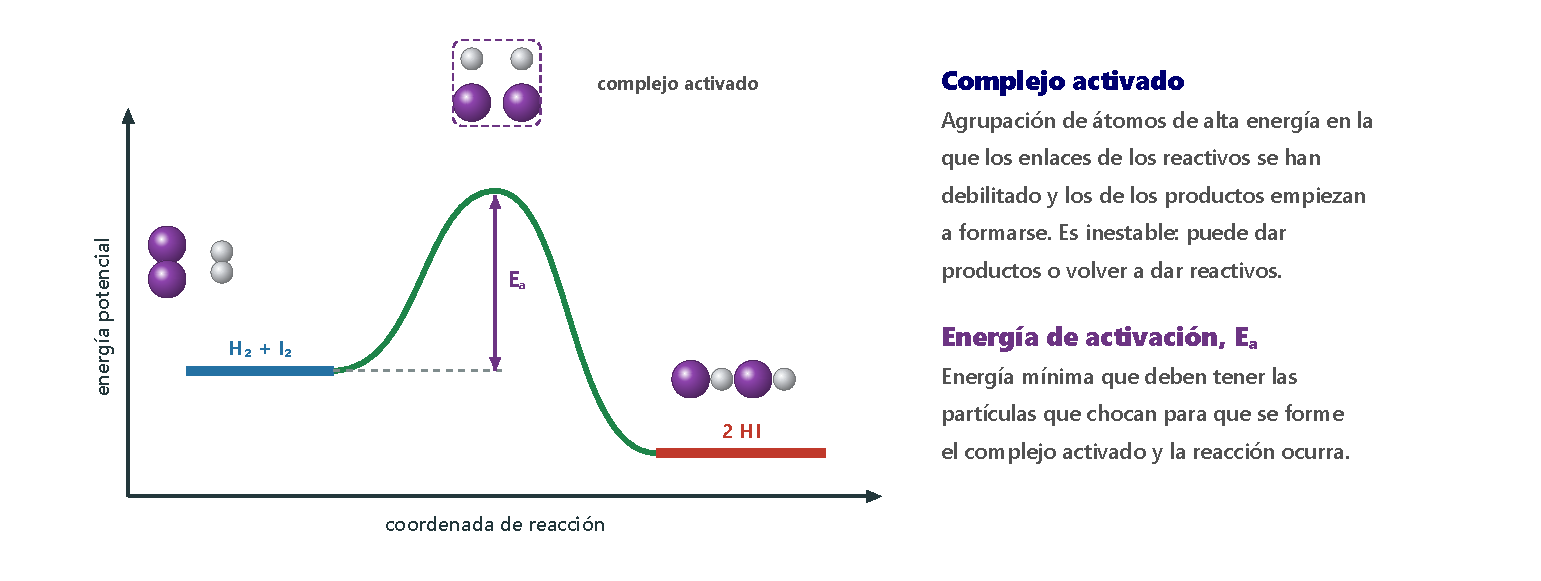
\includegraphics[width=\textwidth]{images/UD6/complejo_activado}
    \caption{Diagrama de energía de la reacción \ch{H2 + I2 -> 2 HI}.}
    \label{fig:complejo_activado}
\end{figure}

\begin{exercise}
    En la reacción \ch{NO + NO3 -> 2 NO2} la molécula de \ch{NO} tiene que unirse por su átomo de nitrógeno a uno de los oxígenos del \ch{NO3}. Explica cuál de estos choques podría dar lugar a la reacción:
    \begin{enumerate}[label=\alph*)]
        \item El \ch{NO} choca por su oxígeno con el nitrógeno del \ch{NO3}.
        \item El \ch{NO} choca por su nitrógeno con un oxígeno del \ch{NO3}.
        \item El \ch{NO} choca de lado, sin que ningún átomo quede enfrentado a un oxígeno del \ch{NO3}.
    \end{enumerate}
    \begin{solu}
        Solo el choque \textcolor{red}{b)}: es el único con la orientación adecuada, porque el nitrógeno del \ch{NO} queda enfrentado a un oxígeno del \ch{NO3} y puede formarse el enlace \ch{N-O}. (Además, tiene que producirse con energía suficiente.)
    \end{solu}
\end{exercise}

\begin{exercise}
    Relaciona cada concepto con su definición.

    \textbf{Conceptos:} a) Teoría de las colisiones. b) Teoría del estado de transición. c) Complejo activado. d) Energía de activación.

    \textbf{Definiciones:} A. Energía mínima necesaria para que reaccionen dos partículas que chocan con la orientación adecuada. B. Para que haya reacción, las partículas deben chocar con energía suficiente y orientación adecuada. C. Los átomos pasan por una distribución de enlaces menos estable que la de los reactivos y los productos. D. Agrupación de alta energía en la que los enlaces de los reactivos se han debilitado y los de los productos han empezado a formarse.
    \begin{solu}
        \textcolor{red}{a--B; b--C; c--D; d--A.}
    \end{solu}
\end{exercise}

\begin{exercise}
    Queremos subir una piedra desde un valle (A) hasta el otro lado de una colina, a un valle más bajo (B), pasando por la cima (C). ¿En qué se parece este trayecto al diagrama de energía de una reacción química?
    \begin{solu}
        La piedra en A son los \textcolor{red}{reactivos}; la cima C, el \textcolor{red}{complejo activado}; el valle B, los \textcolor{red}{productos}. Aunque B está más bajo que A, para llegar hay que «subir» primero la colina: esa subida es la \textcolor{red}{energía de activación}.
    \end{solu}
\end{exercise}

\begin{exercise}
    Indica qué enlaces se rompen y cuáles se forman en estas reacciones, y de qué tipo es cada enlace:
    \begin{enumerate}[label=\alph*)]
        \item \ch{H2 (g) + Br2 (g) -> 2 HBr (g)}
        \item \ch{2 H2 (g) + O2 (g) -> 2 H2O (g)}
        \item \ch{C (grafito) + O2 (g) -> CO2 (g)}
        \item \ch{Zn (s) + 2 HCl (aq) -> ZnCl2 (aq) + H2 (g)}
    \end{enumerate}
    \begin{solu}
        a) Se rompen \ch{H-H} y \ch{Br-Br}; se forman \ch{H-Br}. Todos \textcolor{red}{covalentes}.
        b) Se rompen \ch{H-H} y \ch{O=O}; se forman \ch{O-H}. Todos \textcolor{red}{covalentes}.
        c) Se rompen los enlaces \ch{C-C} del cristal de grafito (\textcolor{red}{covalente reticular}) y el \ch{O=O} (covalente); se forman \ch{C=O} (covalentes).
        d) Se rompen los enlaces del zinc (\textcolor{red}{metálico}) y los \ch{H-Cl} (covalentes); se forman la unión entre los iones \ch{Zn^{2+}} y \ch{Cl-} (\textcolor{red}{iónica}) y el \ch{H-H} (covalente).
    \end{solu}
\end{exercise}

\begin{exercise}
    Indica si son verdaderas o falsas y corrige las falsas:
    \begin{enumerate}[label=\alph*)]
        \item Para que haya reacción basta con que las partículas de los reactivos tengan energía suficiente.
        \item El complejo activado se forma cuando los reactivos chocan con energía y orientación adecuadas, y tiene más energía que los reactivos y los productos.
        \item La energía de activación es la energía mínima que necesitan las partículas que chocan con la orientación adecuada para reaccionar.
        \item Los reactivos siempre tienen menos energía que los productos.
    \end{enumerate}
    \begin{solu}
        a) \textcolor{red}{Falsa}: además deben chocar con la orientación adecuada. b) \textcolor{red}{Verdadera}. c) \textcolor{red}{Verdadera}. d) \textcolor{red}{Falsa}: eso solo ocurre en las reacciones endotérmicas; en las exotérmicas los productos tienen menos energía.
    \end{solu}
\end{exercise}

\begin{exercise}
    En la reacción \ch{NO3 (g) + CO (g) -> NO2 (g) + CO2 (g)} se observan tres choques: A) las moléculas se orientan bien pero chocan muy despacio; B) chocan con mucha energía pero el \ch{CO} golpea al nitrógeno; C) chocan con energía y el carbono del \ch{CO} se enfrenta a un oxígeno del \ch{NO3}. ¿Cuál es eficaz? ¿Por qué no lo son los otros?
    \begin{solu}
        Solo es eficaz el \textcolor{red}{C}: tiene energía suficiente y orientación adecuada. En A falta \textcolor{red}{energía} y en B falla la \textcolor{red}{orientación}.
    \end{solu}
\end{exercise}

%========================================================================================
\section{¿Qué sucede con la masa en una reacción química?}
%========================================================================================

En 1774, el químico francés Antoine-Laurent \textbf{Lavoisier} calentó estaño en un recipiente cerrado y comprobó que la masa total no cambiaba: el estaño se combinaba con el oxígeno del aire del recipiente para formar óxido de estaño, y lo que ganaba el metal era exactamente lo que perdía el aire.

\begin{definition}[Ley de conservación de la masa o ley de Lavoisier]
    En una reacción química la masa total del sistema permanece constante: la masa de los reactivos que reaccionan es igual a la masa de los productos que se forman.
\end{definition}

La teoría de las colisiones lo explica: en una reacción \textbf{los átomos no aparecen ni desaparecen}, solo se reorganizan; por tanto, la masa total se conserva (figura~\ref{fig:conservacion_masa}).

\begin{figure}[H]
    \centering
    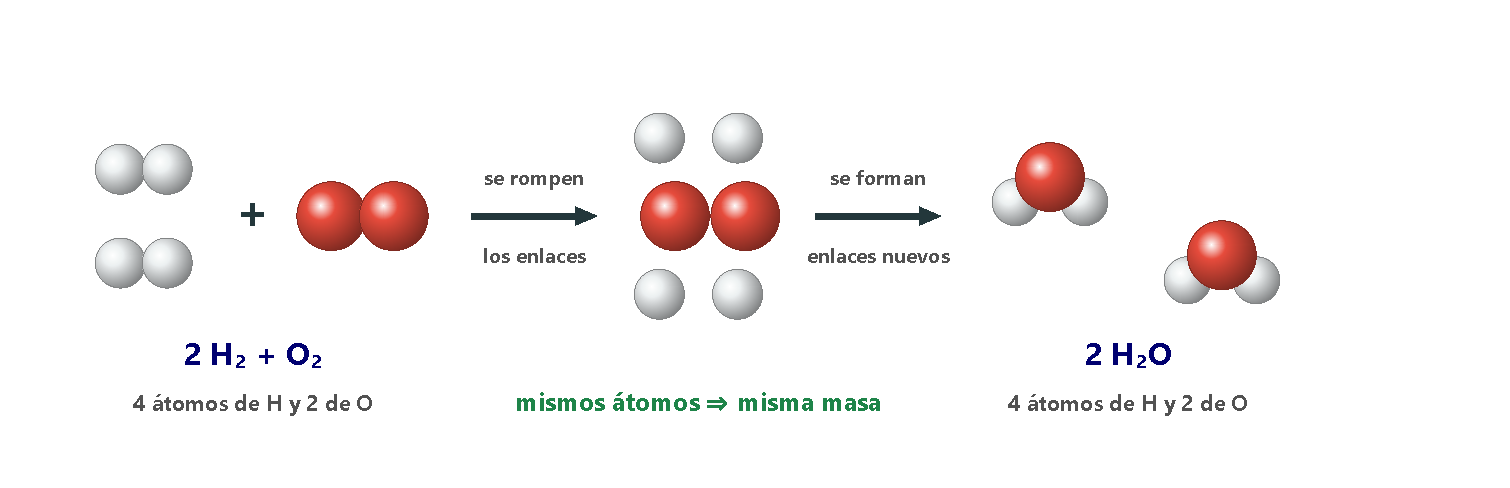
\includegraphics[width=\textwidth]{images/UD6/conservacion_masa}
    \caption{En la reacción \ch{2 H2 + O2 -> 2 H2O} los átomos se reorganizan, pero no cambia su número.}
    \label{fig:conservacion_masa}
\end{figure}

\begin{remark}
    \textbf{Otras dos leyes de las reacciones.} \emph{Ley de las proporciones definidas (Proust):} cuando dos elementos se combinan para formar un compuesto, lo hacen siempre en la misma proporción de masa. \emph{Ley de los volúmenes de combinación (Gay-Lussac):} los volúmenes de los gases que reaccionan y los de los gases que se forman, medidos en las mismas condiciones, están en una relación de números enteros sencillos.
\end{remark}

\begin{exercise}
    Para comprobar la ley de conservación de la masa en la maduración de la fruta, pesamos una manzana en un plato, la dejamos varios días y la volvemos a pesar.
    \begin{enumerate}[label=\alph*)]
        \item ¿Coincidirán la masa inicial y la final?
        \item ¿Qué cambiarías en el experimento?
    \end{enumerate}
    \begin{solu}
        a) \textcolor{red}{No}: la manzana pierde agua y gases (como \ch{CO2}) que escapan al aire, así que la masa final es menor. b) Habría que hacerlo en un \textcolor{red}{recipiente cerrado} para que no se pierdan los productos gaseosos (y controlar la temperatura y la humedad). Entonces la masa total sí se conservaría.
    \end{solu}
\end{exercise}

\begin{exercise}
    Al calentar \qty{23.2}{\gram} de óxido de plata en un recipiente abierto quedan \qty{21.6}{\gram} de plata.
    \begin{enumerate}[label=\alph*)]
        \item ¿Qué masa de oxígeno se ha desprendido?
        \item ¿Qué habría pasado en un recipiente hermético?
    \end{enumerate}
    \begin{solu}
        a) \(m_\text{oxígeno} = \num{23.2} - \num{21.6} = \textcolor{red}{\qty{1.6}{\gram}}\). b) La masa total del recipiente \textcolor{red}{no habría cambiado}, porque el oxígeno habría quedado dentro.
    \end{solu}
\end{exercise}

\begin{exercise}
    ¿Qué masa de carbono reacciona con \qty{16}{\gram} de oxígeno si se forman \qty{22}{\gram} de dióxido de carbono?
    \begin{solu}
        Por la ley de Lavoisier: \(m_\text{C} = 22 - 16 = \textcolor{red}{\qty{6}{\gram}}\).
    \end{solu}
\end{exercise}

%========================================================================================
\section{¿Cómo se escribe una ecuación química?}
%========================================================================================

Una \textbf{ecuación química} representa una reacción. A la izquierda de la flecha se escriben los reactivos y a la derecha los productos, indicando entre paréntesis su estado: (s) sólido, (l) líquido, (g) gas y (aq) disuelto en agua.
\[ \text{REACTIVOS} \longrightarrow \text{PRODUCTOS} \]
Como los átomos se conservan, debe haber el \textbf{mismo número de átomos de cada elemento a los dos lados} de la flecha: la ecuación debe estar \textbf{ajustada} (o igualada).

\begin{marker}
    \textbf{Cómo se ajusta una ecuación química.}
    \begin{enumerate}[label=\arabic*.]
        \item Se elige un elemento y se cuentan sus átomos a cada lado. Si no coinciden, se cambian los \textbf{coeficientes} (los números delante de las fórmulas) hasta igualarlos.
        \item Se repite con los demás elementos. Conviene dejar para el final el hidrógeno y el oxígeno.
        \item Se comprueba que todos los elementos quedan igualados.
        \item \textbf{Nunca se cambian los subíndices} de las fórmulas: cambiarían las sustancias.
    \end{enumerate}
\end{marker}

\begin{example}
    \textbf{Ajusta la ecuación de la combustión del metano:} metano + oxígeno \(\to\) dióxido de carbono + agua.

    \textcolor{blue}{Escribimos la ecuación:} \(\ch{CH4 (g) + O2 (g) -> CO2 (g) + H2O (l)}\).
    \begin{itemize}
        \item C: 1 a la izquierda y 1 a la derecha. Ajustado.
        \item H: 4 a la izquierda y 2 a la derecha. Ponemos un 2 delante del agua:
        \[ \ch{CH4 + O2 -> CO2 + 2 H2O} \]
        \item O: 2 a la izquierda y \(2 + 2 = 4\) a la derecha. Ponemos un 2 delante del oxígeno.
    \end{itemize}
    \[ \textcolor{red}{\ch{CH4 (g) + 2 O2 (g) -> CO2 (g) + 2 H2O (l)}} \]
\end{example}

\begin{exercise}
    Ajusta estas ecuaciones químicas:
    \begin{enumerate}[label=\alph*)]
        \item \ch{Zn (s) + AgNO3 (aq) -> Ag (s) + Zn(NO3)2 (aq)}
        \item \ch{HCl (aq) + ZnS (s) -> ZnCl2 (aq) + H2S (g)}
        \item \ch{BaCl2 (aq) + Na2SO4 (aq) -> BaSO4 (s) + NaCl (aq)}
        \item \ch{NO (g) + O2 (g) -> NO2 (g)}
        \item \ch{C3H8 (g) + O2 (g) -> CO2 (g) + H2O (l)}
        \item \ch{H2SO4 (aq) + KOH (aq) -> K2SO4 (aq) + H2O (l)}
    \end{enumerate}
    \begin{solu}
        \textcolor{blue}{Los coeficientes añadidos son los que no valen 1:}

        a) \ch{Zn + 2 AgNO3 -> 2 Ag + Zn(NO3)2}
        \quad b) \ch{2 HCl + ZnS -> ZnCl2 + H2S}
        \quad c) \ch{BaCl2 + Na2SO4 -> BaSO4 + 2 NaCl}

        d) \ch{2 NO + O2 -> 2 NO2}
        \quad e) \ch{C3H8 + 5 O2 -> 3 CO2 + 4 H2O}
        \quad f) \ch{H2SO4 + 2 KOH -> K2SO4 + 2 H2O}
    \end{solu}
\end{exercise}

\begin{exercise}
    Escribe y ajusta las ecuaciones de estas reacciones:
    \begin{enumerate}[label=\alph*)]
        \item calcio + oxígeno \(\to\) óxido de calcio (\ch{CaO});
        \item sodio + oxígeno \(\to\) óxido de sodio (\ch{Na2O});
        \item carbonato de calcio (\ch{CaCO3}) \(\to\) óxido de calcio + dióxido de carbono;
        \item hierro + oxígeno \(\to\) trióxido de dihierro (\ch{Fe2O3});
        \item nitrógeno + hidrógeno \(\to\) amoníaco (\ch{NH3}).
    \end{enumerate}
    \begin{solu}
        a) \ch{2 Ca (s) + O2 (g) -> 2 CaO (s)}
        \quad b) \ch{4 Na (s) + O2 (g) -> 2 Na2O (s)}
        \quad c) \ch{CaCO3 (s) -> CaO (s) + CO2 (g)}

        d) \ch{4 Fe (s) + 3 O2 (g) -> 2 Fe2O3 (s)}
        \quad e) \ch{N2 (g) + 3 H2 (g) -> 2 NH3 (g)}
    \end{solu}
\end{exercise}

%========================================================================================
\section{Estequiometría de las reacciones químicas}
%========================================================================================

Los coeficientes de una ecuación ajustada indican la \textbf{proporción en moles} (y, si son gases en las mismas condiciones, en volumen) en que reaccionan y se forman las sustancias. Por ejemplo:
\[ \ch{N2 (g) + 3 H2 (g) -> 2 NH3 (g)} \]
significa que \qty{1}{\mol} de \ch{N2} reacciona con \qty{3}{\mol} de \ch{H2} para dar \qty{2}{\mol} de \ch{NH3}. Con esta proporción podemos calcular la cantidad de reactivos necesaria para obtener una cantidad de producto, o al revés. Estos cálculos se llaman \textbf{estequiométricos}.

\begin{remark}
    \textbf{Masas atómicas para los cálculos de esta unidad:} H = 1; C = 12; N = 14; O = 16; Na = 23; Mg = 24; Al = 27; S = 32; Cl = \num{35.5}; K = 39; Ca = 40; Fe = 56; Cu = \num{63.5}; Zn = \num{65.4}; Ag = 108; I = 127. Recuerda que un mol de cualquier gas ocupa \qty{22.4}{\L} a \qty{0}{\celsius} y \qty{1}{\atm}.
\end{remark}

\begin{marker}
    \textbf{Pasos de un cálculo estequiométrico.}
    \begin{enumerate}[label=\arabic*.]
        \item Escribe y ajusta la ecuación química.
        \item Escribe debajo de cada sustancia la proporción en moles que indican los coeficientes.
        \item Pasa a moles el dato conocido (con la masa molar, el volumen molar o la molaridad).
        \item Con la proporción de la ecuación, calcula los moles de la sustancia pedida.
        \item Pasa esos moles a la magnitud que se pide (masa, volumen, número de partículas\ldots).
    \end{enumerate}
\end{marker}

\begin{example}
    \textbf{¿Qué masa de óxido de hierro(III) se obtiene al oxidar por completo \qty{56}{\gram} de hierro?}

    \textcolor{blue}{1 y 2.} \(\ch{4 Fe (s) + 3 O2 (g) -> 2 Fe2O3 (s)}\): \quad \qty{4}{\mol} de Fe dan \qty{2}{\mol} de \ch{Fe2O3}.

    \textcolor{blue}{3.} \(n(\ch{Fe}) = \dfrac{\qty{56}{\gram}}{\qty{56}{\gram\per\mol}} = \qty{1}{\mol}\).
    \qquad \textcolor{blue}{4.} \(n(\ch{Fe2O3}) = \qty{1}{\mol}\,\ch{Fe} \cdot \dfrac{\qty{2}{\mol}\,\ch{Fe2O3}}{\qty{4}{\mol}\,\ch{Fe}} = \qty{0.5}{\mol}\).

    \textcolor{blue}{5.} \(M(\ch{Fe2O3}) = 2 \cdot 56 + 3 \cdot 16 = \qty{160}{\gram\per\mol}\); \quad \(m = \num{0.5} \cdot 160 = \textcolor{red}{\qty{80}{\gram}}\).
\end{example}

\paragraph{El rendimiento de una reacción.} En la práctica casi nunca se obtiene toda la cantidad de producto que predicen los cálculos: hay reacciones secundarias, pérdidas al recoger el producto, reactivos impuros\ldots{} Por eso se define el \textbf{rendimiento}:
\[ \text{rendimiento}\,(\%) = \frac{\text{cantidad de producto obtenida}}{\text{cantidad de producto teórica}} \cdot 100 \]
En el ejemplo anterior, si el rendimiento fuera del \qty{80}{\percent}, obtendríamos \(80 \cdot \frac{80}{100} = \qty{64}{\gram}\) de \ch{Fe2O3}.

\begin{example}
    \textbf{Cálculos con disoluciones.} ¿Qué volumen de disolución de \ch{NaOH} \num{0.5} M hace falta para neutralizar \qty{100}{\mL} de \ch{HCl} \num{0.2} M?

    \textcolor{blue}{Ecuación:} \(\ch{HCl (aq) + NaOH (aq) -> NaCl (aq) + H2O (l)}\): proporción 1:1.

    \textcolor{blue}{Moles de HCl:} \(n = M \cdot V = \num{0.2} \cdot \num{0.100} = \qty{0.02}{\mol}\) \(\Rightarrow\) hacen falta \qty{0.02}{\mol} de \ch{NaOH}.

    \textcolor{blue}{Volumen:} \(V = \dfrac{n}{M} = \dfrac{\num{0.02}}{\num{0.5}} = \textcolor{red}{\qty{0.040}{\L} = \qty{40}{\mL}}\).
\end{example}

\begin{exercise}
    El magnesio reacciona con el oxígeno para dar óxido de magnesio.
    \begin{enumerate}[label=\alph*)]
        \item Escribe la ecuación ajustada.
        \item ¿Qué volumen de oxígeno, a \qty{0}{\celsius} y \qty{1}{\atm}, hace falta para obtener \qty{120}{\gram} de óxido de magnesio?
    \end{enumerate}
    \begin{solu}
        a) \ch{2 Mg (s) + O2 (g) -> 2 MgO (s)}.
        b) \(M(\ch{MgO}) = \qty{40}{\gram\per\mol}\); \(n(\ch{MgO}) = \frac{120}{40} = \qty{3}{\mol}\). Por la ecuación, \(n(\ch{O2}) = \frac{3}{2} = \qty{1.5}{\mol}\); \(V = \num{1.5} \cdot \num{22.4} = \textcolor{red}{\qty{33.6}{\L}}\).
    \end{solu}
\end{exercise}

\begin{exercise}
    El cloro y el hidrógeno reaccionan para dar cloruro de hidrógeno. ¿Qué volumen de \ch{H2} hace falta para obtener \qty{44.8}{\L} de \ch{HCl}, si todos los gases se miden a \qty{0}{\celsius} y \qty{1}{\atm}?
    \begin{solu}
        \ch{H2 (g) + Cl2 (g) -> 2 HCl (g)}. Por cada 2 volúmenes de \ch{HCl} hace falta 1 de \ch{H2}: \(V(\ch{H2}) = \frac{\num{44.8}}{2} = \textcolor{red}{\qty{22.4}{\L}}\) (\qty{1}{\mol}).
    \end{solu}
\end{exercise}

\begin{exercise}
    Al calentarlo, el carbonato de calcio se descompone en óxido de calcio y dióxido de carbono. Si se descomponen \qty{150}{\gram} de \ch{CaCO3} con un rendimiento del \qty{80}{\percent}:
    \begin{enumerate}[label=\alph*)]
        \item ¿Qué masa de \ch{CaO} se obtiene?
        \item ¿Qué volumen de \ch{CO2}, a \qty{0}{\celsius} y \qty{1}{\atm}, se desprende?
    \end{enumerate}
    \begin{solu}
        \ch{CaCO3 (s) -> CaO (s) + CO2 (g)} (1:1:1). \(M(\ch{CaCO3}) = \qty{100}{\gram\per\mol}\); \(n = \frac{150}{100} = \qty{1.5}{\mol}\).
        a) Teórico: \(\num{1.5} \cdot 56 = \qty{84}{\gram}\) de \ch{CaO}; real: \(84 \cdot \num{0.80} = \textcolor{red}{\qty{67.2}{\gram}}\).
        b) Teórico: \(\num{1.5} \cdot \num{22.4} = \qty{33.6}{\L}\); real: \(\num{33.6} \cdot \num{0.80} = \textcolor{red}{\qty{26.9}{\L}}\) de \ch{CO2}.
    \end{solu}
\end{exercise}

\begin{exercise}
    El ácido clorhídrico reacciona con el hidróxido de potasio para dar cloruro de potasio y agua. ¿Qué volumen de \ch{KOH} \num{0.5} M reacciona exactamente con \qty{150}{\mL} de \ch{HCl} \num{0.2} M?
    \begin{solu}
        \ch{HCl + KOH -> KCl + H2O} (1:1). \(n(\ch{HCl}) = \num{0.2} \cdot \num{0.150} = \qty{0.03}{\mol} = n(\ch{KOH})\); \(V = \frac{\num{0.03}}{\num{0.5}} = \textcolor{red}{\qty{0.060}{\L} = \qty{60}{\mL}}\).
    \end{solu}
\end{exercise}

\begin{exercise}
    El trióxido de azufre se obtiene según la ecuación (sin ajustar) \ch{SO2 (g) + O2 (g) -> SO3 (g)}.
    \begin{enumerate}[label=\alph*)]
        \item Ajusta la ecuación.
        \item ¿Qué masa de \ch{SO2} reacciona con \qty{16}{\gram} de \ch{O2}?
        \item ¿Qué masa de \ch{SO3} se obtiene en ese caso?
        \item ¿Qué volumen de \ch{SO3} se obtiene a partir de \qty{11.2}{\L} de \ch{SO2}, si ambos se miden a \qty{0}{\celsius} y \qty{1}{\atm}?
    \end{enumerate}
    \begin{solu}
        a) \ch{2 SO2 (g) + O2 (g) -> 2 SO3 (g)}.
        b) \(n(\ch{O2}) = \frac{16}{32} = \qty{0.5}{\mol}\) \(\Rightarrow\) \(n(\ch{SO2}) = \qty{1}{\mol}\); \(m = 1 \cdot 64 = \textcolor{red}{\qty{64}{\gram}}\).
        c) \(n(\ch{SO3}) = \qty{1}{\mol}\); \(m = 1 \cdot 80 = \textcolor{red}{\qty{80}{\gram}}\) (comprueba: \(64 + 16 = 80\)).
        d) La proporción en volumen \ch{SO2}:\ch{SO3} es 2:2: se obtienen \textcolor{red}{\qty{11.2}{\L}} de \ch{SO3}.
    \end{solu}
\end{exercise}

\begin{exercise}
    El carbonato de calcio se descompone a alta temperatura en óxido de calcio (cal viva) y dióxido de carbono.
    \begin{enumerate}[label=\alph*)]
        \item Escribe la ecuación ajustada.
        \item ¿Qué masa de \ch{CaCO3} hace falta para obtener \qty{560}{\kg} de \ch{CaO} si el rendimiento es del \qty{100}{\percent}?
        \item ¿Qué volumen de \ch{CO2}, a \qty{0}{\celsius} y \qty{1}{\atm}, se desprende en ese caso?
        \item ¿Qué masa de \ch{CaCO3} hace falta para obtener \qty{112}{\kg} de \ch{CaO} si el rendimiento es del \qty{80}{\percent}?
        \item ¿Qué masa de \ch{CaO} se obtiene a partir de \qty{50}{\kg} de \ch{CaCO3} con ese mismo rendimiento?
    \end{enumerate}
    \begin{solu}
        a) \ch{CaCO3 (s) -> CaO (s) + CO2 (g)}.
        b) \(n(\ch{CaO}) = \frac{\num{560000}}{56} = \qty{10000}{\mol} = n(\ch{CaCO3})\); \(m = \num{10000} \cdot 100 = \qty{e6}{\gram} = \textcolor{red}{\qty{1000}{\kg}}\).
        c) \(n(\ch{CO2}) = \qty{10000}{\mol}\); \(V = \num{10000} \cdot \num{22.4} = \textcolor{red}{\qty{224000}{\L}}\) (\qty{224}{\cubic\metre}).
        d) Teóricamente harían falta \(\frac{\num{112000}}{56} \cdot 100 = \qty{200}{\kg}\); como solo reacciona el \qty{80}{\percent}, hay que poner más: \(\frac{200}{\num{0.80}} = \textcolor{red}{\qty{250}{\kg}}\).
        e) Teórico: \(\frac{\num{50000}}{100} \cdot 56 = \qty{28}{\kg}\); real: \(28 \cdot \num{0.80} = \textcolor{red}{\qty{22.4}{\kg}}\).
    \end{solu}
\end{exercise}

\begin{exercise}
    Calcula el volumen de oxígeno, a \qty{0}{\celsius} y \qty{1}{\atm}, necesario para quemar por completo el butano de una bombona de \qty{11.6}{\kg}:
    \[ \ch{2 C4H10 (g) + 13 O2 (g) -> 8 CO2 (g) + 10 H2O (g)} \]
    \begin{solu}
        \(M(\ch{C4H10}) = 48 + 10 = \qty{58}{\gram\per\mol}\); \(n = \frac{\num{11600}}{58} = \qty{200}{\mol}\).
        \(n(\ch{O2}) = 200 \cdot \frac{13}{2} = \qty{1300}{\mol}\); \(V = 1300 \cdot \num{22.4} = \textcolor{red}{\qty{29120}{\L}}\) (unos \qty{29}{\cubic\metre}).
    \end{solu}
\end{exercise}

\begin{exercise}
    Calcula el volumen de hidrógeno, a \qty{0}{\celsius} y \qty{1}{\atm}, que se desprende al hacer reaccionar \qty{13.08}{\gram} de zinc con suficiente ácido clorhídrico. Ecuación sin ajustar: \ch{Zn (s) + HCl (aq) -> ZnCl2 (aq) + H2 (g)}.
    \begin{solu}
        \ch{Zn + 2 HCl -> ZnCl2 + H2}. \(n(\ch{Zn}) = \frac{\num{13.08}}{\num{65.4}} = \qty{0.2}{\mol} = n(\ch{H2})\); \(V = \num{0.2} \cdot \num{22.4} = \textcolor{red}{\qty{4.48}{\L}}\).
    \end{solu}
\end{exercise}

\begin{exercise}
    El sodio reacciona violentamente con el agua: \ch{2 Na (s) + 2 H2O (l) -> 2 NaOH (aq) + H2 (g)}. ¿Qué masa de \ch{NaOH} se forma con \qty{2.3}{\gram} de sodio?
    \begin{solu}
        \(n(\ch{Na}) = \frac{\num{2.3}}{23} = \qty{0.1}{\mol} = n(\ch{NaOH})\); \(m = \num{0.1} \cdot 40 = \textcolor{red}{\qty{4}{\gram}}\).
    \end{solu}
\end{exercise}

\begin{exercise}
    Se oxidan por completo \qty{54}{\gram} de aluminio para dar óxido de aluminio, \ch{Al2O3}.
    \begin{enumerate}[label=\alph*)]
        \item Escribe la ecuación ajustada.
        \item ¿Qué volumen de oxígeno, a \qty{0}{\celsius} y \qty{1}{\atm}, se necesita?
        \item ¿Qué masa de óxido se obtiene?
    \end{enumerate}
    \begin{solu}
        a) \ch{4 Al (s) + 3 O2 (g) -> 2 Al2O3 (s)}.
        b) \(n(\ch{Al}) = \frac{54}{27} = \qty{2}{\mol}\); \(n(\ch{O2}) = 2 \cdot \frac{3}{4} = \qty{1.5}{\mol}\); \(V = \textcolor{red}{\qty{33.6}{\L}}\).
        c) \(n(\ch{Al2O3}) = 2 \cdot \frac{2}{4} = \qty{1}{\mol}\); \(M = 54 + 48 = \qty{102}{\gram\per\mol}\); \(m = \textcolor{red}{\qty{102}{\gram}}\).
    \end{solu}
\end{exercise}

\begin{exercise}
    El amoníaco se descompone en nitrógeno e hidrógeno, ambos gaseosos.
    \begin{enumerate}[label=\alph*)]
        \item Escribe la ecuación ajustada.
        \item ¿Qué volumen de \ch{H2} se obtiene al descomponer \qty{34}{\gram} de \ch{NH3}?
        \item ¿Y de \ch{N2}?
    \end{enumerate}
    (Volúmenes medidos a \qty{0}{\celsius} y \qty{1}{\atm}.)
    \begin{solu}
        a) \ch{2 NH3 (g) -> N2 (g) + 3 H2 (g)}.
        b) \(n(\ch{NH3}) = \frac{34}{17} = \qty{2}{\mol}\); \(n(\ch{H2}) = 3\,\unit{\mol}\); \(V = 3 \cdot \num{22.4} = \textcolor{red}{\qty{67.2}{\L}}\).
        c) \(n(\ch{N2}) = \qty{1}{\mol}\); \(V = \textcolor{red}{\qty{22.4}{\L}}\).
    \end{solu}
\end{exercise}

\begin{exercise}
    Cuando el zinc reacciona con ácido clorhídrico se forma cloruro de zinc y se desprende hidrógeno.
    \begin{enumerate}[label=\alph*)]
        \item Escribe y ajusta la ecuación.
        \item ¿Cuántos moles de \ch{HCl} reaccionan con \qty{0.5}{\mol} de zinc?
        \item ¿Qué volumen de hidrógeno, a \qty{0}{\celsius} y \qty{1}{\atm}, se obtiene a partir de \qty{32.7}{\gram} de zinc?
    \end{enumerate}
    \begin{solu}
        a) \ch{Zn (s) + 2 HCl (aq) -> ZnCl2 (aq) + H2 (g)}. b) \(\textcolor{red}{\qty{1}{\mol}}\) de \ch{HCl}. c) \(n(\ch{Zn}) = \frac{\num{32.7}}{\num{65.4}} = \qty{0.5}{\mol} = n(\ch{H2})\); \(V = \textcolor{red}{\qty{11.2}{\L}}\).
    \end{solu}
\end{exercise}

\begin{exercise}
    El carbonato de cobre(II) se descompone al calentarlo: \ch{CuCO3 (s) -> CuO (s) + CO2 (g)}. Se descomponen \qty{24.7}{\gram} de \ch{CuCO3} con un rendimiento del \qty{80}{\percent}.
    \begin{enumerate}[label=\alph*)]
        \item ¿Qué masa de \ch{CO2} se obtiene?
        \item ¿Qué volumen ocupa a \qty{0}{\celsius} y \qty{1}{\atm}?
        \item ¿Qué masa de óxido de cobre(II) se forma?
    \end{enumerate}
    \begin{solu}
        \(M(\ch{CuCO3}) = \num{63.5} + 12 + 48 = \qty{123.5}{\gram\per\mol}\); \(n = \frac{\num{24.7}}{\num{123.5}} = \qty{0.2}{\mol}\). Con el rendimiento, se forman \(\num{0.2} \cdot \num{0.80} = \qty{0.16}{\mol}\) de cada producto.
        a) \(m(\ch{CO2}) = \num{0.16} \cdot 44 = \textcolor{red}{\qty{7.04}{\gram}}\). b) \(V = \num{0.16} \cdot \num{22.4} = \textcolor{red}{\qty{3.58}{\L}}\). c) \(m(\ch{CuO}) = \num{0.16} \cdot \num{79.5} = \textcolor{red}{\qty{12.72}{\gram}}\).
    \end{solu}
\end{exercise}

%========================================================================================
\section{¿Con qué velocidad transcurre una reacción química?}
%========================================================================================

Algunas reacciones son muy rápidas, como la combustión del butano, y otras muy lentas, como la oxidación del hierro o del cobre.

\begin{definition}[Velocidad de reacción]
    Es la cantidad de sustancia que se transforma (o que se forma) por unidad de tiempo. Puede medirse a partir de la cantidad de reactivo que desaparece o de producto que aparece en cada unidad de tiempo.
\end{definition}

Estudiemos la reacción del carbonato de calcio con ácido clorhídrico, midiendo el volumen de \ch{CO2} que se recoge en una probeta invertida sobre agua:
\[ \ch{CaCO3 (s) + 2 HCl (aq) -> CaCl2 (aq) + CO2 (g) + H2O (l)} \]

\begin{center}
    % --- tabla antigua ---
    % \begin{tblr}{colspec={lcccccccc}, hlines, vlines, column{1}={bg=ocre!85, fg=white, font=\bfseries}, cells={font=\small}}
        % Tiempo (\unit{\minute}) & 0 & 1 & 2 & 3 & 4 & 5 & 6 & 7 \\
        % \(V_{\ch{CO2}}\) con \ch{CaCO3} en trozos (\unit{\cubic\centi\metre}) & 0 & \num{15.25} & --- & \num{26.20} & --- & \num{29.25} & \num{30.25} & \num{30.50} \\
        % \(V_{\ch{CO2}}\) con \ch{CaCO3} pulverizado (\unit{\cubic\centi\metre}) & 0 & \num{22.40} & \num{28.00} & \num{30.25} & \num{30.50} & \num{30.50} & \num{30.50} & \num{30.50} \\
    % \end{tblr}
    % --- tabla nueva ---
    {\small
    \begin{tabular}{@{}lcccccccc@{}}
        \toprule
        \textbf{Tiempo (\unit{\minute})} & 0 & 1 & 2 & 3 & 4 & 5 & 6 & 7 \\[3pt]
        \textbf{\(V_{\ch{CO2}}\) con \ch{CaCO3} en trozos (\unit{\cubic\centi\metre})} & 0 & \num{15.25} & --- & \num{26.20} & --- & \num{29.25} & \num{30.25} & \num{30.50} \\[3pt]
        \textbf{\(V_{\ch{CO2}}\) con \ch{CaCO3} pulverizado (\unit{\cubic\centi\metre})} & 0 & \num{22.40} & \num{28.00} & \num{30.25} & \num{30.50} & \num{30.50} & \num{30.50} & \num{30.50} \\
        \bottomrule
    \end{tabular}
    }
\end{center}

La velocidad es muy alta al principio y va disminuyendo a medida que se gastan los reactivos. La \textbf{velocidad media} con los trozos durante los 7 minutos es \(v_m = \dfrac{\qty{30.5}{\cubic\centi\metre}}{\qty{7}{\minute}} = \qty{4.36}{\cubic\centi\metre\per\minute}\).

\subsection{¿Qué factores influyen en la velocidad de una reacción?}

\begin{itemize}
    \item \textbf{La superficie de contacto.} Cuanto más dividido está un reactivo sólido, más rápida es la reacción: con el carbonato pulverizado se obtiene el mismo volumen de \ch{CO2} en mucho menos tiempo.
    \item \textbf{La concentración de los reactivos.} La velocidad aumenta al aumentar la concentración: con ácido clorhídrico más concentrado la reacción es más rápida.
    \item \textbf{La temperatura.} En general, la velocidad aumenta con la temperatura. Por eso conservamos los alimentos en el frigorífico.
    \item \textbf{Los catalizadores.} Un \textbf{catalizador} es una sustancia distinta de los reactivos y de los productos que modifica la velocidad de la reacción y se recupera íntegra al final; por eso no aparece en la ecuación química. Los catalizadores \textbf{positivos} la aceleran y los \textbf{negativos} (o inhibidores) la frenan.
\end{itemize}

\begin{figure}[H]
    \centering
    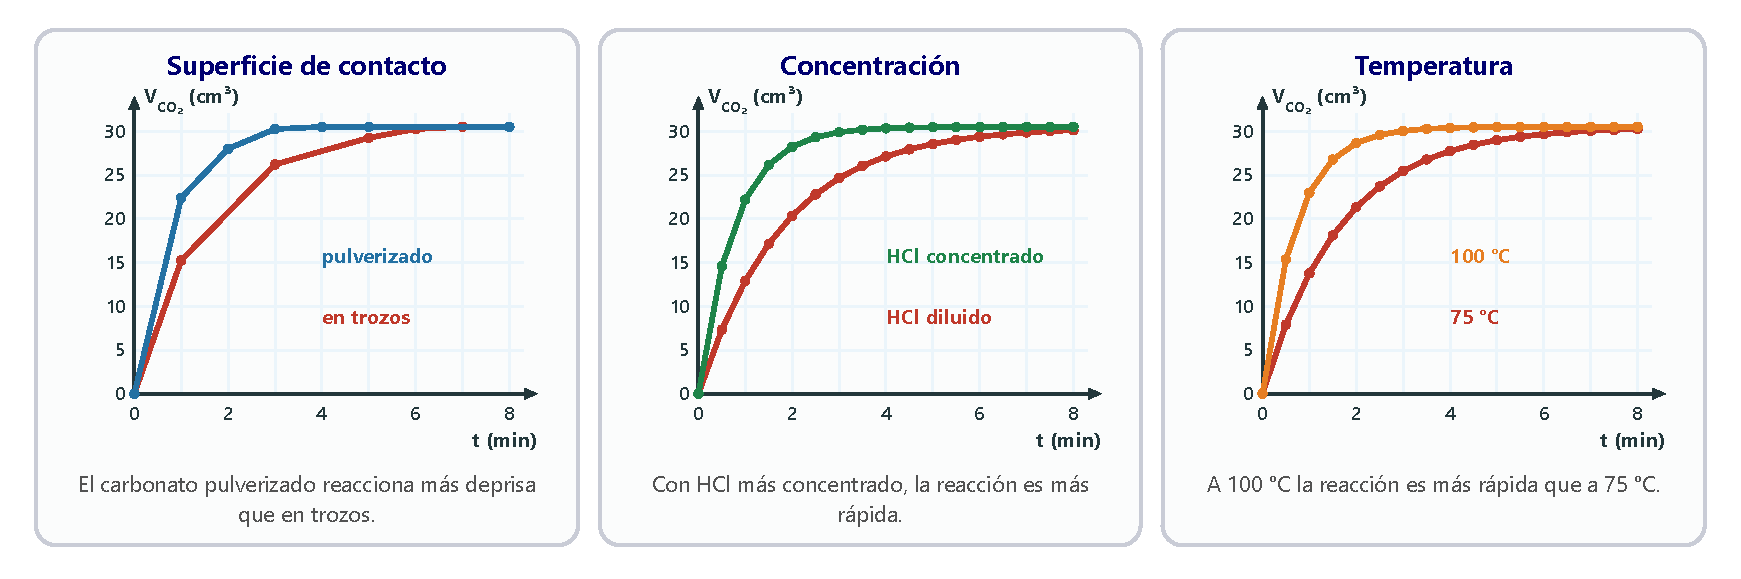
\includegraphics[width=\textwidth]{images/UD6/factores_velocidad}
    \caption{Volumen de \ch{CO2} desprendido frente al tiempo al variar la superficie de contacto, la concentración del ácido y la temperatura.}
    \label{fig:factores_velocidad}
\end{figure}

\paragraph{¿Cómo lo explica la teoría de las colisiones?} La velocidad depende del número de \textbf{choques eficaces} por unidad de tiempo (figura~\ref{fig:particulas_velocidad}):
\begin{itemize}
    \item Si el sólido está más dividido, hay más partículas en la superficie que pueden chocar.
    \item Si la concentración es mayor, hay más partículas en el mismo volumen y chocan más a menudo.
    \item Si la temperatura es mayor, las partículas se mueven más deprisa: chocan más veces y una proporción mayor de los choques tiene la energía suficiente.
    \item Un catalizador positivo permite que la reacción transcurra por un camino con un complejo activado de \textbf{menor energía de activación}; uno negativo, por un camino de mayor energía de activación (figura~\ref{fig:catalizador}).
\end{itemize}

\begin{figure}[H]
    \centering
    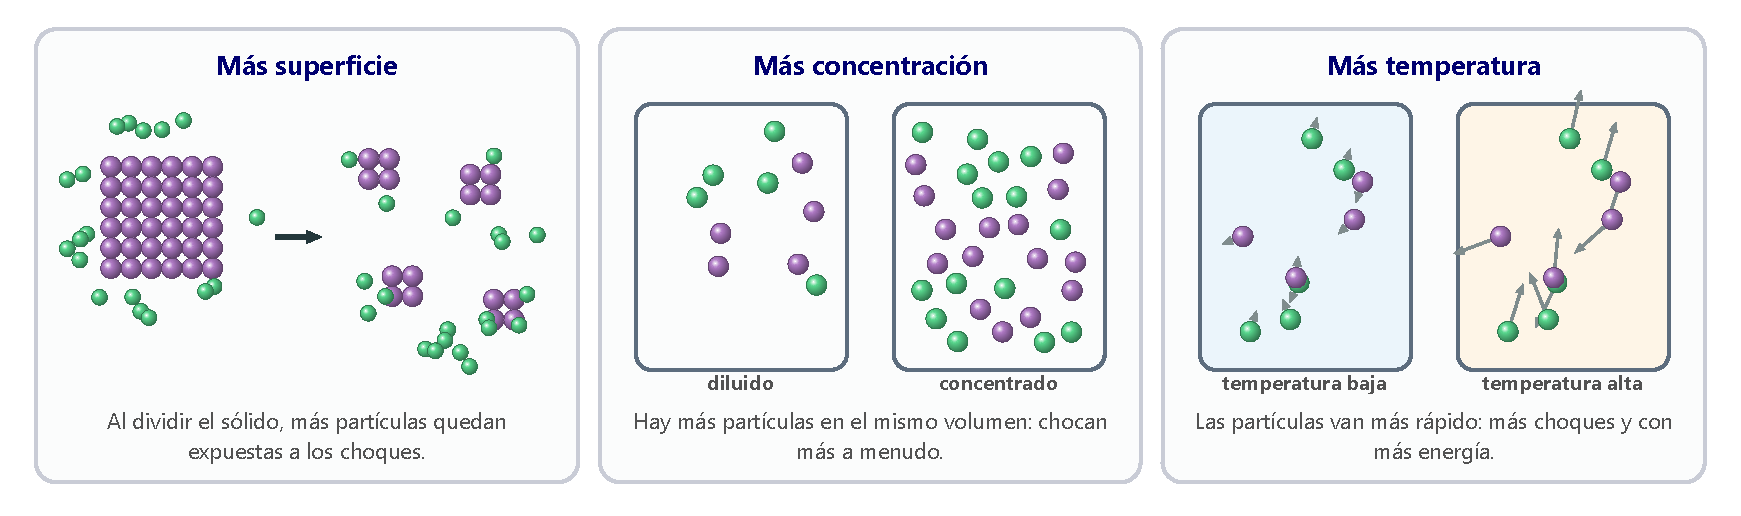
\includegraphics[width=\textwidth]{images/UD6/particulas_velocidad}
    \caption{Interpretación de los factores que afectan a la velocidad con el modelo de partículas.}
    \label{fig:particulas_velocidad}
\end{figure}

\begin{figure}[H]
    \centering
    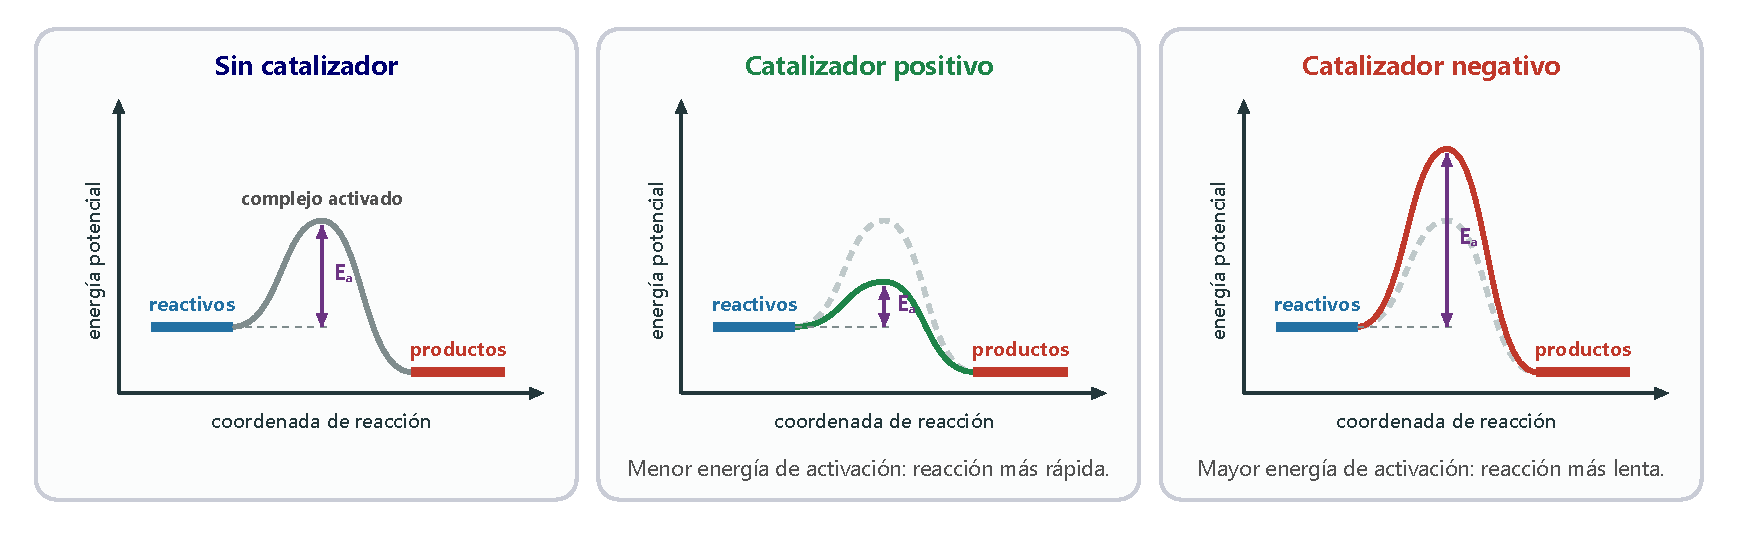
\includegraphics[width=\textwidth]{images/UD6/catalizador}
    \caption{Los catalizadores modifican la energía de activación de una reacción.}
    \label{fig:catalizador}
\end{figure}

\begin{exercise}
    Con los datos de la tabla, ¿qué volumen de \ch{CO2} se ha obtenido a los 3 minutos en cada experimento? ¿Cuál ha sido la velocidad media de la reacción hasta ese momento?
    \begin{solu}
        En trozos: \qty{26.20}{\cubic\centi\metre}; \(v_m = \frac{\num{26.20}}{3} = \textcolor{red}{\qty{8.73}{\cubic\centi\metre\per\minute}}\). Pulverizado: \qty{30.25}{\cubic\centi\metre}; \(v_m = \frac{\num{30.25}}{3} = \textcolor{red}{\qty{10.08}{\cubic\centi\metre\per\minute}}\).
    \end{solu}
\end{exercise}

\begin{exercise}
    Usa la gráfica de la superficie de contacto (figura~\ref{fig:factores_velocidad}) para responder:
    \begin{enumerate}[label=\alph*)]
        \item ¿Qué volumen de \ch{CO2} se ha obtenido a los 5 minutos en cada caso?
        \item ¿Cuánto tiempo hace falta, aproximadamente, para obtener \qty{15}{\cubic\centi\metre} de \ch{CO2} en cada caso?
        \item ¿Cuál es la velocidad media durante los dos primeros minutos con el carbonato pulverizado? ¿Coincide con la velocidad media de toda la reacción?
    \end{enumerate}
    \begin{solu}
        a) En trozos, \textcolor{red}{\qty{29.25}{\cubic\centi\metre}}; pulverizado, \textcolor{red}{\qty{30.50}{\cubic\centi\metre}} (la reacción ya ha terminado).
        b) En trozos, \textcolor{red}{alrededor de \qty{1}{\minute}}; pulverizado, \textcolor{red}{unos \qty{0.7}{\minute}} (40 segundos).
        c) \(v_m = \frac{28}{2} = \textcolor{red}{\qty{14}{\cubic\centi\metre\per\minute}}\). \textcolor{red}{No}: la velocidad media de toda la reacción es menor, porque la reacción se va frenando a medida que se gastan los reactivos.
    \end{solu}
\end{exercise}

\begin{exercise}
    ¿Por qué la carne picada se estropea antes que la misma cantidad de carne en un solo trozo?
    \begin{solu}
        Porque está más dividida: tiene \textcolor{red}{más superficie de contacto} con el aire y los microorganismos, y las reacciones de descomposición son más rápidas.
    \end{solu}
\end{exercise}

\begin{exercise}
    Algunas manchas desaparecen al tratarlas con lejía. ¿Cómo afectará a la velocidad de esta reacción usar lejía más concentrada? ¿Y lavar la prenda con agua caliente?
    \begin{solu}
        En los dos casos la reacción será \textcolor{red}{más rápida}: al aumentar la concentración hay más choques entre partículas, y al aumentar la temperatura los choques son más frecuentes y más energéticos. (También se decolorará antes el tejido.)
    \end{solu}
\end{exercise}

\begin{exercise}
    ¿Cómo influye la temperatura en la conservación de los alimentos frescos?
    \begin{solu}
        Al bajar la temperatura \textcolor{red}{disminuye la velocidad} de las reacciones de descomposición; por eso los alimentos se conservan más tiempo en el frigorífico o en el congelador.
    \end{solu}
\end{exercise}

\begin{exercise}
    Investiga para qué sirve el catalizador del tubo de escape de los coches.
    \begin{solu}
        Respuesta libre. Acelera reacciones que transforman gases tóxicos de la combustión (\ch{CO}, óxidos de nitrógeno, hidrocarburos sin quemar) en gases menos dañinos (\ch{CO2}, \ch{N2}, \ch{H2O}).
    \end{solu}
\end{exercise}

\begin{exercise}
    El agua oxigenada se descompone muy lentamente: \ch{2 H2O2 (aq) -> 2 H2O (l) + O2 (g)}. Recoger \qty{50}{\cubic\centi\metre} de oxígeno lleva cientos de días; pero si se añade \qty{1}{\gram} de dióxido de manganeso, \ch{MnO2}, basta con unos minutos.
    \begin{enumerate}[label=\alph*)]
        \item Explica lo que ocurre.
        \item ¿Se gasta el dióxido de manganeso?
    \end{enumerate}
    \begin{solu}
        a) El \ch{MnO2} actúa como \textcolor{red}{catalizador positivo}: disminuye la energía de activación y la reacción se acelera. b) \textcolor{red}{No}: al final se recupera el gramo de \ch{MnO2} sin cambios.
    \end{solu}
\end{exercise}

\begin{exercise}
    Al mezclar ácido clorhídrico con tiosulfato de sodio se forma un precipitado amarillo de azufre. Colocamos el vaso sobre un papel con una cruz dibujada y medimos el tiempo que tarda en dejar de verse la cruz. Repetimos el experimento con las mismas concentraciones a distintas temperaturas:
    \begin{center}
        % --- tabla antigua ---
        % \begin{tblr}{colspec={lcccc}, hlines, vlines, column{1}={bg=ocre!85, fg=white, font=\bfseries}}
            % Temperatura (\unit{\celsius}) & 15 & 25 & 35 & 45 \\
            % Tiempo (\unit{\second}) & 240 & 130 & 60 & 35 \\
        % \end{tblr}
        % --- tabla nueva ---
        \begin{tabular}{@{}lcccc@{}}
            \toprule
            \textbf{Temperatura (\unit{\celsius})} & 15 & 25 & 35 & 45 \\[3pt]
            \textbf{Tiempo (\unit{\second})} & 240 & 130 & 60 & 35 \\
            \bottomrule
        \end{tabular}
    \end{center}
    \begin{enumerate}[label=\alph*)]
        \item ¿Qué conclusión sacas sobre la velocidad de la reacción?
        \item ¿Por qué hay que mantener constantes las concentraciones?
    \end{enumerate}
    \begin{solu}
        a) Cuanto mayor es la temperatura, menos tarda en desaparecer la cruz: la velocidad \textcolor{red}{aumenta con la temperatura}.
        b) Porque queremos estudiar solo el efecto de la temperatura: es la \textcolor{red}{variable independiente}, y la concentración es una variable controlada. Si cambiaran las dos a la vez, no sabríamos a cuál se debe el efecto.
    \end{solu}
\end{exercise}

\begin{exercise}
    Lee el texto y responde:

    \begin{quote}
        \emph{Una mezcla de hidrógeno y oxígeno puede estar en un recipiente durante años sin cambio aparente: a temperatura ambiente reaccionan, pero con una lentitud extraordinaria. Si se calienta, las paredes se empañan de agua, y a unos \qty{550}{\celsius} la mezcla explota. Hace más de un siglo se comprobó que, si se introduce un alambre de platino en la mezcla fría, la reacción se completa en segundos y el platino sale intacto.}
    \end{quote}

    \begin{enumerate}[label=\alph*)]
        \item ¿Una explosión es una reacción exotérmica o endotérmica?
        \item ¿Cómo es la velocidad de la reacción a temperatura ambiente? ¿Y a \qty{550}{\celsius}?
        \item Escribe la ecuación ajustada de formación del agua.
        \item ¿Qué factores influyen en su velocidad según el texto? ¿Qué papel tiene el platino?
    \end{enumerate}
    \begin{solu}
        a) \textcolor{red}{Exotérmica}: desprende mucha energía y gases muy rápidamente.
        b) A temperatura ambiente es \textcolor{red}{extremadamente lenta}; a \qty{550}{\celsius} es \textcolor{red}{explosiva}.
        c) \ch{2 H2 (g) + O2 (g) -> 2 H2O (g)}.
        d) La \textcolor{red}{temperatura} y la presencia de un \textcolor{red}{catalizador}: el platino acelera la reacción y no se gasta.
    \end{solu}
\end{exercise}

%========================================================================================
\section{Reacciones exotérmicas y endotérmicas}
%========================================================================================

Si añadimos ácido clorhídrico a unas limaduras de zinc, la temperatura sube y el vaso se calienta. En toda reacción química se desprende o se absorbe energía, normalmente en forma de calor, de luz o de electricidad.

\begin{definition}[Reacciones exotérmicas y endotérmicas]
    Una reacción es \textbf{exotérmica} si \textbf{desprende} energía, y \textbf{endotérmica} si la \textbf{absorbe}. El \textbf{calor de reacción} es la energía en forma de calor que se desprende o se absorbe en una reacción.
\end{definition}

En una reacción exotérmica los productos tienen \textbf{menos} energía que los reactivos, y la diferencia se desprende. En una endotérmica los productos tienen \textbf{más} energía, y la diferencia hay que aportarla (figura~\ref{fig:exo_endo}).

\begin{figure}[H]
    \centering
    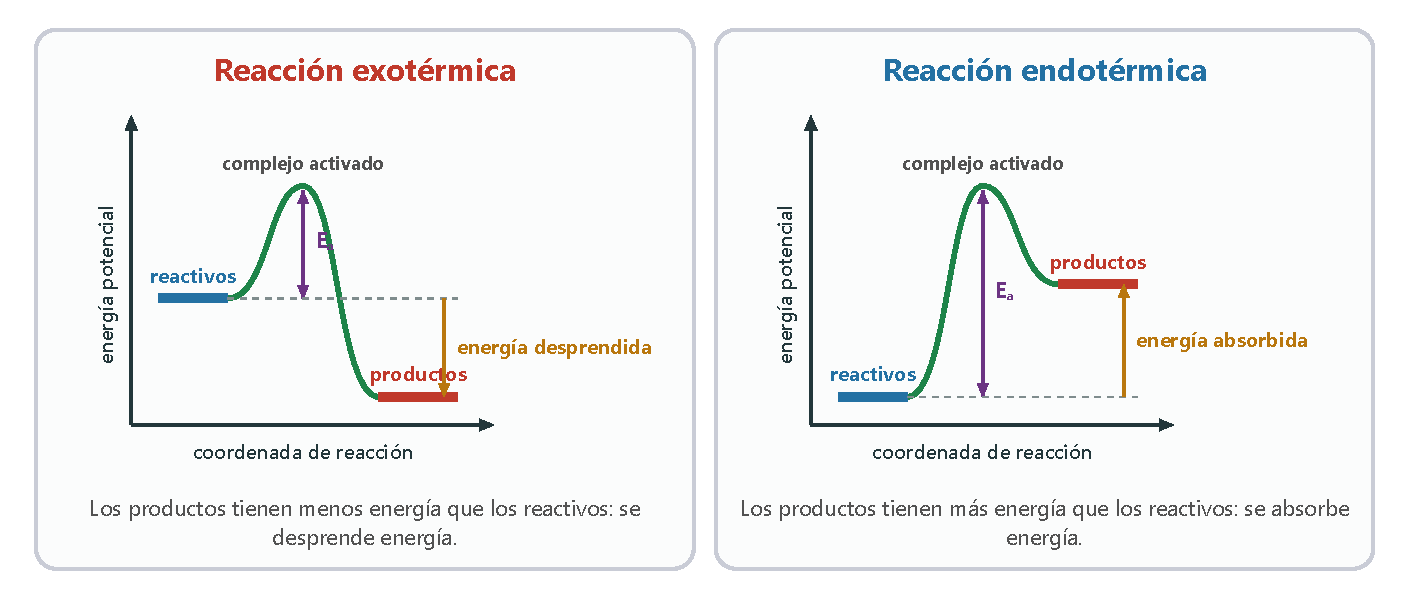
\includegraphics[width=0.9\textwidth]{images/UD6/exo_endo}
    \caption{Diagramas de energía de una reacción exotérmica y de una endotérmica.}
    \label{fig:exo_endo}
\end{figure}

\subsection{Ecuaciones termoquímicas}

Una \textbf{ecuación termoquímica} es una ecuación química ajustada en la que se indica la energía desprendida o absorbida y el estado físico de todas las sustancias. Por convenio, la energía es \textbf{negativa} si la reacción es \textbf{exotérmica} y \textbf{positiva} si es \textbf{endotérmica}:
\begin{align*}
    &\ch{H2 (g) + 1/2 O2 (g) -> H2O (g)} \qquad \text{calor de reacción} = \qty{-241.8}{\kilo\joule\per\mol} \\
    &\ch{CaCO3 (s) -> CaO (s) + CO2 (g)} \qquad \text{calor de reacción} = \qty{+178}{\kilo\joule\per\mol}
\end{align*}
La primera indica que al formarse \qty{1}{\mol} de agua se desprenden \qty{241.8}{\kilo\joule}; la segunda, que para descomponer \qty{1}{\mol} de carbonato de calcio hay que aportar \qty{178}{\kilo\joule}.

\begin{remark}
    \textbf{Reacciones reversibles e irreversibles.} Una reacción es \textbf{reversible} si, a medida que se forman los productos, estos reaccionan entre sí y vuelven a dar los reactivos; se llega a un \emph{equilibrio} dinámico y se escribe con una doble flecha: \(\ch{H2 + I2 <=> 2 HI}\). Es \textbf{irreversible} si los productos no reaccionan entre sí, como cuando se forma un precipitado que se separa: \(\ch{AgNO3 (aq) + NaCl (aq) -> AgCl (s) v + NaNO3 (aq)}\).
\end{remark}

\begin{exercise}
    Clasifica estas reacciones en exotérmicas y endotérmicas:
    \begin{enumerate}[label=\alph*)]
        \item \ch{N2 + 3 H2 -> 2 NH3}; calor de reacción: \qty{-92}{\kilo\joule}
        \item \ch{N2 + O2 -> 2 NO}; calor de reacción: \qty{+181}{\kilo\joule}
        \item \ch{2 SO2 + O2 -> 2 SO3}; calor de reacción: \qty{-198}{\kilo\joule}
        \item \ch{2 H2O -> 2 H2 + O2}; calor de reacción: \qty{+484}{\kilo\joule}
    \end{enumerate}
    \begin{solu}
        Exotérmicas (energía negativa): \textcolor{red}{a) y c)}. Endotérmicas (energía positiva): \textcolor{red}{b) y d)}.
    \end{solu}
\end{exercise}

\begin{exercise}
    Con la ecuación termoquímica de formación del agua, ¿qué energía se desprende al formarse \qty{1.5}{\mol} de agua? ¿Y al reaccionar \qty{4}{\gram} de hidrógeno?
    \begin{solu}
        \(\num{1.5} \cdot \num{241.8} = \textcolor{red}{\qty{362.7}{\kilo\joule}}\). \qty{4}{\gram} de \ch{H2} son \qty{2}{\mol}, que forman \qty{2}{\mol} de agua: \(2 \cdot \num{241.8} = \textcolor{red}{\qty{483.6}{\kilo\joule}}\).
    \end{solu}
\end{exercise}

\begin{exercise}
    Indica si son verdaderas o falsas y corrige las falsas:
    \begin{enumerate}[label=\alph*)]
        \item Una reacción exotérmica absorbe energía.
        \item En una reacción exotérmica la energía se considera positiva.
        \item En una reacción endotérmica la energía se considera negativa.
        \item El calor de reacción es la energía que se absorbe o se desprende en una reacción.
        \item Si el calor de reacción es \qty{-125}{\kilo\joule\per\mol}, se absorben \qty{125}{\kilo\joule} por mol.
        \item En una reacción exotérmica los productos tienen menos energía que los reactivos.
        \item En una reacción endotérmica los productos tienen menos energía que los reactivos.
    \end{enumerate}
    \begin{solu}
        a) \textcolor{red}{Falsa}: la \emph{desprende}. b) \textcolor{red}{Falsa}: se considera \emph{negativa}. c) \textcolor{red}{Falsa}: se considera \emph{positiva}. d) \textcolor{red}{Verdadera}. e) \textcolor{red}{Falsa}: se \emph{desprenden} \qty{125}{\kilo\joule} por mol. f) \textcolor{red}{Verdadera}. g) \textcolor{red}{Falsa}: tienen \emph{más} energía.
    \end{solu}
\end{exercise}

\begin{exercise}
    Dibuja el diagrama de energía de una reacción exotérmica y el de una endotérmica. Indica en ellos: a) las magnitudes de los ejes; b) dónde están los reactivos y los productos; c) la energía de activación; d) la energía desprendida o absorbida.
    \begin{solu}
        Como los de la figura~\ref{fig:exo_endo}: a) eje vertical, \textcolor{red}{energía}; eje horizontal, \textcolor{red}{coordenada (avance) de la reacción}. b) Reactivos a la izquierda y productos a la derecha; en la exotérmica los productos quedan más abajo y en la endotérmica, más arriba. c) La energía de activación es la altura desde los reactivos hasta la cima (complejo activado). d) La energía desprendida o absorbida es la diferencia de altura entre reactivos y productos.
    \end{solu}
\end{exercise}

\begin{exercise}
    Para la reacción \ch{H2 (g) + Cl2 (g) -> 2 HCl (g)} se desprenden \qty{184}{\kilo\joule}.
    \begin{enumerate}[label=\alph*)]
        \item ¿Es exotérmica o endotérmica?
        \item ¿Qué energía se desprende al formarse \qty{1}{\mol} de \ch{HCl}? ¿Y \qty{3}{\mol}?
        \item Dibuja su diagrama de energía.
    \end{enumerate}
    \begin{solu}
        a) \textcolor{red}{Exotérmica}. b) Por mol de \ch{HCl}: \(\frac{184}{2} = \textcolor{red}{\qty{92}{\kilo\joule}}\); para \qty{3}{\mol}: \(3 \cdot 92 = \textcolor{red}{\qty{276}{\kilo\joule}}\). c) Como el diagrama exotérmico de la figura~\ref{fig:exo_endo}, con \ch{H2 + Cl2} a la izquierda, \ch{2 HCl} \qty{184}{\kilo\joule} más abajo a la derecha.
    \end{solu}
\end{exercise}

\begin{exercise}
    La combustión del carbono es \ch{C (s) + O2 (g) -> CO2 (g)}, con un calor de reacción de \qty{-393.5}{\kilo\joule\per\mol}.
    \begin{enumerate}[label=\alph*)]
        \item ¿Es exotérmica o endotérmica?
        \item ¿Qué energía se desprende al quemar \qty{500}{\gram} de carbono?
    \end{enumerate}
    \begin{solu}
        a) \textcolor{red}{Exotérmica}. b) \(n = \frac{500}{12} = \qty{41.67}{\mol}\); \(E = \num{41.67} \cdot \num{393.5} = \textcolor{red}{\qty{16397}{\kilo\joule}}\) (unos \qty{1.64e4}{\kilo\joule}).
    \end{solu}
\end{exercise}

\begin{exercise}
    En la combustión del metano se desprenden \qty{890}{\kilo\joule\per\mol}, y en la del butano, \qty{2876}{\kilo\joule\per\mol}. Si quemamos \qty{500}{\gram} de cada combustible, ¿cuál desprende más energía?
    \begin{solu}
        Metano (\(M = \qty{16}{\gram\per\mol}\)): \(\frac{500}{16} = \qty{31.25}{\mol}\); \(\num{31.25} \cdot 890 = \qty{27813}{\kilo\joule}\).
        Butano (\(M = \qty{58}{\gram\per\mol}\)): \(\frac{500}{58} = \qty{8.62}{\mol}\); \(\num{8.62} \cdot 2876 = \qty{24793}{\kilo\joule}\).
        Desprende más energía el \textcolor{red}{metano}, aunque por mol desprenda menos.
    \end{solu}
\end{exercise}

\begin{exercise}
    En el diagrama de energía de la reacción \ch{2 NOCl -> 2 NO + Cl2} los productos están por encima de los reactivos. En el de la reacción \ch{NO + O3 -> NO2 + O2} los productos están por debajo. ¿Cuál es exotérmica y cuál endotérmica?
    \begin{solu}
        La primera es \textcolor{red}{endotérmica} (los productos tienen más energía) y la segunda, \textcolor{red}{exotérmica} (los productos tienen menos energía).
    \end{solu}
\end{exercise}

%========================================================================================
\section{Tipos de reacciones químicas}
%========================================================================================

A diario se producen centenares de reacciones: en los laboratorios y en la industria, pero también en la atmósfera, en la cocina o en nuestro cuerpo. Muchas de ellas pueden clasificarse en unos pocos tipos.

\subsection{Reacciones de síntesis}

En una reacción de \textbf{síntesis} dos o más sustancias reaccionan para dar una única sustancia nueva.

\begin{center}
    % --- tabla antigua ---
    % \begin{tblr}{colspec={X[c]X[c]}, hlines, vlines, row{1}={bg=ocre!85, fg=white, font=\bfseries}, rowsep=2pt}
        % A partir de sus elementos & A partir de otros compuestos \\
        % {No metal + metal \(\to\) sal binaria \\ \ch{Cl2 (g) + 2 Na (s)} \(\rightarrow\) \ch{2 NaCl (s)}} & {Óxido de metal + agua \(\to\) hidróxido \\ \ch{CaO (s) + H2O (l)} \(\rightarrow\) \ch{Ca(OH)2 (aq)}} \\
        % {Metal + oxígeno \(\to\) óxido de metal \\ \ch{2 Mg (s) + O2 (g)} \(\rightarrow\) \ch{2 MgO (s)}} & {Óxido de no metal + agua \(\to\) oxoácido \\ \ch{SO3 (g) + H2O (l)} \(\rightarrow\) \ch{H2SO4 (aq)}} \\
        % {No metal + oxígeno \(\to\) óxido de no metal \\ \ch{2 H2 (g) + O2 (g)} \(\rightarrow\) \ch{2 H2O (l)}} & {Compuesto + elemento \(\to\) nuevo compuesto \\ \ch{PCl3 (g) + Cl2 (g)} \(\rightarrow\) \ch{PCl5 (g)}} \\
        % {No metal + no metal \(\to\) hidruro no metálico \\ \ch{N2 (g) + 3 H2 (g)} \(\rightarrow\) \ch{2 NH3 (g)}} & \\
    % \end{tblr}
    % --- tabla nueva ---
    \begin{tabular}{@{}C{0.45\linewidth} C{0.45\linewidth}@{}}
        \toprule
        \textbf{A partir de sus elementos} & \textbf{A partir de otros compuestos} \\
        \midrule
        No metal + metal \(\to\) sal binaria \newline \ch{Cl2 (g) + 2 Na (s)} \(\rightarrow\) \ch{2 NaCl (s)} & Óxido de metal + agua \(\to\) hidróxido \newline \ch{CaO (s) + H2O (l)} \(\rightarrow\) \ch{Ca(OH)2 (aq)} \\[3pt]
        Metal + oxígeno \(\to\) óxido de metal \newline \ch{2 Mg (s) + O2 (g)} \(\rightarrow\) \ch{2 MgO (s)} & Óxido de no metal + agua \(\to\) oxoácido \newline \ch{SO3 (g) + H2O (l)} \(\rightarrow\) \ch{H2SO4 (aq)} \\[3pt]
        No metal + oxígeno \(\to\) óxido de no metal \newline \ch{2 H2 (g) + O2 (g)} \(\rightarrow\) \ch{2 H2O (l)} & Compuesto + elemento \(\to\) nuevo compuesto \newline \ch{PCl3 (g) + Cl2 (g)} \(\rightarrow\) \ch{PCl5 (g)} \\[3pt]
        No metal + no metal \(\to\) hidruro no metálico \newline \ch{N2 (g) + 3 H2 (g)} \(\rightarrow\) \ch{2 NH3 (g)} &  \\
        \bottomrule
    \end{tabular}
\end{center}

\subsection{Reacciones de oxidación y de reducción}

Los objetos de hierro que están a la intemperie se cubren de herrumbre si no se protegen con pintura. Es una \textbf{oxidación}.
\begin{itemize}
    \item Una \textbf{oxidación} es una reacción en la que una sustancia \textbf{gana oxígeno}:
    \[ \ch{2 Fe (s) + O2 (g) -> 2 FeO (s)} \qquad \ch{2 Cu (s) + O2 (g) -> 2 CuO (s)} \]
    \item Una \textbf{reducción} es una reacción en la que un compuesto \textbf{pierde oxígeno}.
\end{itemize}
La oxidación y la reducción ocurren siempre a la vez. En la reacción
\[ \ch{CuO (s) + H2 (g) -> Cu (s) + H2O (g)} \]
el óxido de cobre(II) \textbf{se reduce} (pierde oxígeno) y el hidrógeno \textbf{se oxida} (lo gana). El hidrógeno es el \textbf{agente reductor} y el óxido de cobre, el \textbf{agente oxidante}. En realidad, estas reacciones son \textbf{transferencias de electrones}: la sustancia que cede electrones se oxida y la que los capta se reduce. Por eso se llaman reacciones \textbf{redox}.

\begin{remark}
    \textbf{El enranciamiento y la corrosión.} La mantequilla, el aceite o el vino se \emph{enrancian} al oxidarse; por eso se guardan en lugares frescos y oscuros, y muchos alimentos llevan antioxidantes. La \emph{corrosión} es la oxidación del hierro y del acero no protegidos: destruye estructuras metálicas y prevenirla tiene un coste elevado.
\end{remark}

\subsection{Los procesos electroquímicos}

Los procesos \textbf{electroquímicos} transforman energía química en eléctrica, o al revés (figura~\ref{fig:pila_electrolisis}).
\begin{itemize}
    \item \textbf{Las pilas.} En una reacción redox hay una transferencia de electrones. Si la oxidación y la reducción tienen lugar en sitios separados y unidos por un circuito, los electrones circulan por él: se produce una corriente eléctrica continua. Es una \textbf{pila}. En la \emph{pila alcalina}, el zinc del electrodo negativo se oxida a \ch{Zn^{2+}} y el dióxido de manganeso, en contacto con la barra de grafito del electrodo positivo, capta los electrones y se reduce.
    \item \textbf{La electrólisis.} Si hacemos pasar corriente eléctrica a través de un compuesto iónico fundido o disuelto (el \textbf{electrolito}), se produce una reacción química, inversa a la de una pila. Hacen falta un generador de corriente continua, el electrolito, una cuba electrolítica y dos electrodos (cátodo y ánodo). La electrólisis del agua produce hidrógeno y oxígeno: \(\ch{2 H2O (l) -> 2 H2 (g) + O2 (g)}\).
\end{itemize}

\begin{figure}[H]
    \centering
    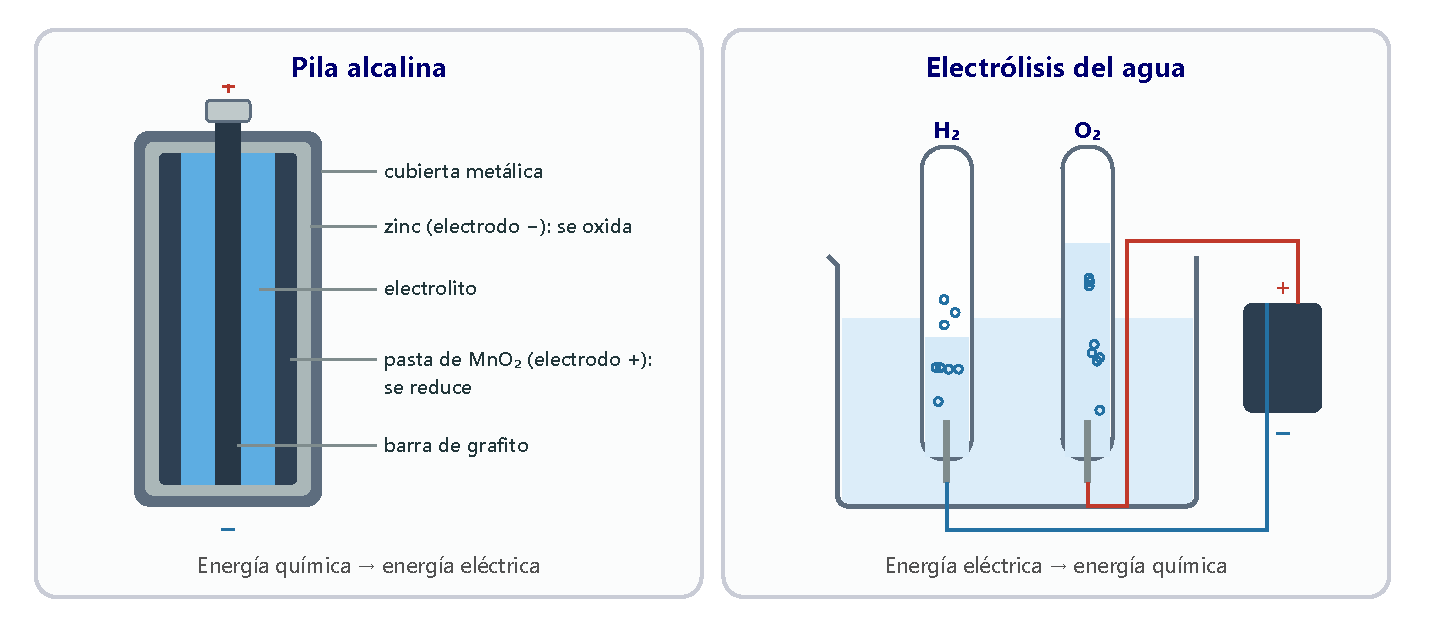
\includegraphics[width=0.95\textwidth]{images/UD6/pila_electrolisis}
    \caption{Una pila transforma energía química en eléctrica; la electrólisis hace lo contrario.}
    \label{fig:pila_electrolisis}
\end{figure}

\paragraph{Aplicaciones de la electrólisis.} Permite obtener elementos a partir de sus compuestos: cobre muy puro, hidrógeno para usarlo como combustible («hidrógeno verde» si la electricidad es renovable), o metales como el aluminio, el sodio o el magnesio. También se usa en la \textbf{galvanoplastia}: recubrir un objeto metálico con otro metal (plata, oro, níquel) para decorarlo o protegerlo, colocándolo como cátodo en una disolución con iones de ese metal.

\subsection{Ácidos y bases}

El químico sueco Svante \textbf{Arrhenius} (1859-1927) dio la primera definición de ácido y de base basándose en su disociación en agua:

\begin{center}
    % --- tabla antigua ---
    % \begin{tblr}{colspec={X[l]X[l]}, hlines, vlines, row{1}={bg=ocre!85, fg=white, font=\bfseries, halign=c}}
        % Ácido & Base \\
        % {Sustancia que en disolución acuosa se disocia dando \textbf{iones hidrógeno}, \ch{H+}: \\ \ch{HCl (aq)} \(\rightarrow\) \ch{H+ (aq) + Cl- (aq)}} & {Sustancia que en disolución acuosa se disocia dando \textbf{iones hidróxido}, \ch{OH-}: \\ \ch{NaOH (aq)} \(\rightarrow\) \ch{Na+ (aq) + OH- (aq)}} \\
        % Sabor ácido. Reaccionan con metales como el zinc o el magnesio desprendiendo hidrógeno. Reaccionan con las bases para dar sales. & Sabor amargo. Reaccionan con los ácidos para dar sales. Reaccionan con las grasas formando jabones. \\
        % Ejemplos: ácido clorhídrico, nítrico, sulfúrico, acético (vinagre)\ldots & Ejemplos: amoníaco, hidróxidos de los metales alcalinos y alcalinotérreos\ldots \\
    % \end{tblr}
    % --- tabla nueva ---
    \begin{tabular}{@{}L{0.45\linewidth} L{0.45\linewidth}@{}}
        \toprule
        \textbf{Ácido} & \textbf{Base} \\
        \midrule
        Sustancia que en disolución acuosa se disocia dando \textbf{iones hidrógeno}, \ch{H+}: \newline \ch{HCl (aq)} \(\rightarrow\) \ch{H+ (aq) + Cl- (aq)} & Sustancia que en disolución acuosa se disocia dando \textbf{iones hidróxido}, \ch{OH-}: \newline \ch{NaOH (aq)} \(\rightarrow\) \ch{Na+ (aq) + OH- (aq)} \\[3pt]
        Sabor ácido. Reaccionan con metales como el zinc o el magnesio desprendiendo hidrógeno. Reaccionan con las bases para dar sales. & Sabor amargo. Reaccionan con los ácidos para dar sales. Reaccionan con las grasas formando jabones. \\[3pt]
        Ejemplos: ácido clorhídrico, nítrico, sulfúrico, acético (vinagre)\ldots & Ejemplos: amoníaco, hidróxidos de los metales alcalinos y alcalinotérreos\ldots \\
        \bottomrule
    \end{tabular}
\end{center}

\paragraph{La escala de pH.} Es una escala numérica, normalmente entre 0 y 14, que indica el grado de acidez o basicidad de una disolución (figura~\ref{fig:escala_ph}):
\begin{itemize}
    \item pH = 7: disolución \textbf{neutra}.
    \item pH < 7: disolución \textbf{ácida} (cuanto menor, más ácida).
    \item pH > 7: disolución \textbf{básica} (cuanto mayor, más básica).
\end{itemize}
El pH se mide con \textbf{indicadores} (como la fenolftaleína, incolora en medio ácido y rosa en medio básico), con \textbf{papel indicador}, que cambia de color, o con un \textbf{pH-metro} digital.

\begin{figure}[H]
    \centering
    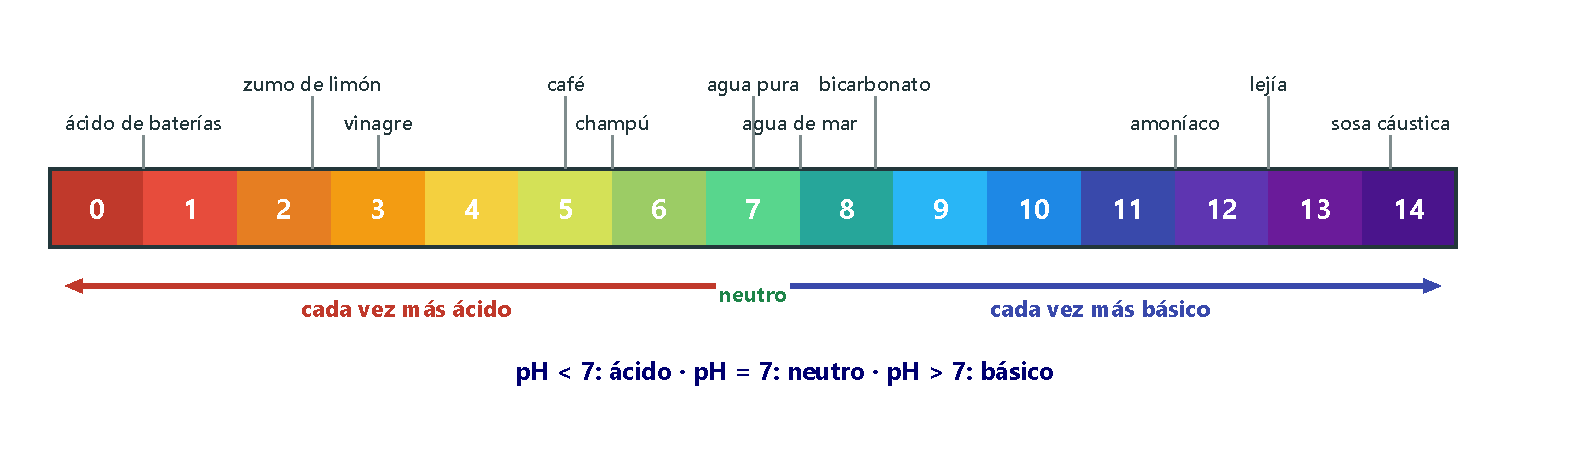
\includegraphics[width=\textwidth]{images/UD6/escala_ph}
    \caption{Escala de pH con algunas sustancias de uso cotidiano.}
    \label{fig:escala_ph}
\end{figure}

\paragraph{La neutralización.} Es la reacción entre un ácido y una base para dar una \textbf{sal y agua}. Si añadimos poco a poco ácido clorhídrico a una disolución de hidróxido de sodio, llega un momento en que la disolución es neutra:
\[ \text{ácido} + \text{base} \longrightarrow \text{sal} + \text{agua} \qquad \ch{HCl (aq) + NaOH (aq) -> NaCl (aq) + H2O (l)} \]

\subsection{Reacciones de combustión}

Una \textbf{combustión} es una oxidación muy rápida en la que una sustancia (el combustible) reacciona con el oxígeno y se desprende mucha energía: es una reacción \textbf{exotérmica}. Por eso se usa para obtener energía en los hogares, los motores, la industria y las centrales térmicas. Los combustibles más usados son el metano (gas natural), el propano, el butano, la gasolina, el gasóleo y otros derivados del petróleo.
\begin{itemize}
    \item Combustión del carbono: \(\ch{C (s) + O2 (g) -> CO2 (g)} + \text{energía}\)
    \item Combustión de un hidrocarburo: \(\ch{CH4 (g) + 2 O2 (g) -> CO2 (g) + 2 H2O (l)} + \text{energía}\)
    \item Respiración celular: \(\ch{C6H12O6 (aq) + 6 O2 (g) -> 6 CO2 (g) + 6 H2O (l)} + \text{energía}\)
\end{itemize}

\paragraph{El efecto invernadero.} Algunos gases de la atmósfera, como el \ch{CO2}, el metano o el vapor de agua, retienen parte del calor que emite la superficie terrestre y lo devuelven hacia ella. Este \textbf{efecto invernadero} natural mantiene una temperatura adecuada para la vida. Pero desde la Revolución Industrial, la quema de combustibles fósiles ha aumentado mucho el \ch{CO2} atmosférico: es el \textbf{incremento del efecto invernadero}, que provoca un aumento de la temperatura media de la Tierra (\textbf{calentamiento global}). Una de sus consecuencias es el \textbf{cambio climático}: un cambio global en las pautas del clima.

\begin{figure}[H]
    \centering
    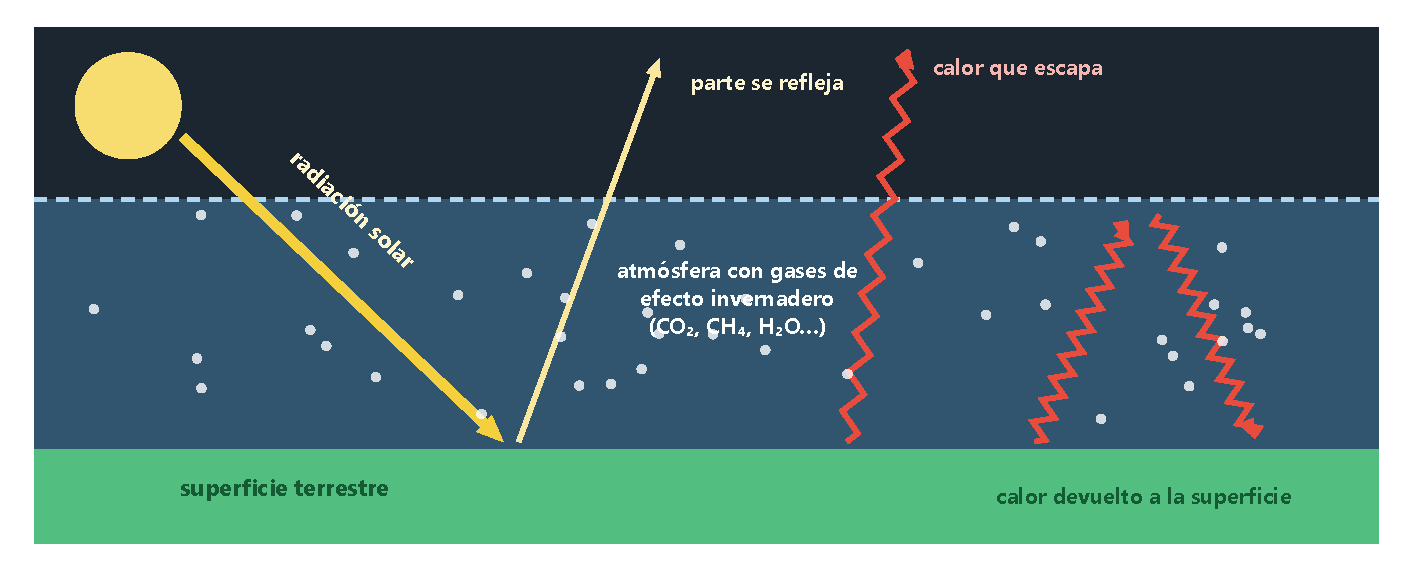
\includegraphics[width=0.9\textwidth]{images/UD6/efecto_invernadero}
    \caption{El efecto invernadero: parte del calor emitido por la Tierra vuelve hacia la superficie.}
    \label{fig:efecto_invernadero}
\end{figure}

\begin{exercise}
    Escribe la ecuación de disociación en agua de estas sustancias e indica cuáles son ácidos y cuáles bases: a) ácido bromhídrico, \ch{HBr}; b) ácido acético, \ch{CH3COOH}; c) hidróxido de sodio, \ch{NaOH}; d) hidróxido de bario, \ch{Ba(OH)2}.
    \begin{solu}
        a) \ch{HBr (aq) -> H+ (aq) + Br- (aq)}: \textcolor{red}{ácido}. b) \ch{CH3COOH (aq) -> H+ (aq) + CH3COO- (aq)}: \textcolor{red}{ácido}. c) \ch{NaOH (aq) -> Na+ (aq) + OH- (aq)}: \textcolor{red}{base}. d) \ch{Ba(OH)2 (aq) -> Ba^{2+} (aq) + 2 OH- (aq)}: \textcolor{red}{base}.
    \end{solu}
\end{exercise}

\begin{exercise}
    Clasifica en ácidas, neutras o básicas estas sustancias según su pH: leche, \num{6.5}; lejía, \num{12.5}; refresco de cola, \num{2.5}; sangre, \num{7.4}; vinagre, 3; agua destilada, 7.
    \begin{solu}
        Ácidas: \textcolor{red}{leche, refresco de cola y vinagre}. Neutra: \textcolor{red}{agua destilada}. Básicas: \textcolor{red}{lejía y sangre}.
    \end{solu}
\end{exercise}

\begin{exercise}
    Escribe una reacción de neutralización con la que se pueda obtener: a) cloruro de potasio; b) bromuro de calcio; c) nitrato de potasio; d) sulfato de sodio.
    \begin{solu}
        a) \ch{HCl (aq) + KOH (aq) -> KCl (aq) + H2O (l)}
        \quad b) \ch{2 HBr (aq) + Ca(OH)2 (aq) -> CaBr2 (aq) + 2 H2O (l)}

        c) \ch{HNO3 (aq) + KOH (aq) -> KNO3 (aq) + H2O (l)}
        \quad d) \ch{H2SO4 (aq) + 2 NaOH (aq) -> Na2SO4 (aq) + 2 H2O (l)}
    \end{solu}
\end{exercise}

\begin{exercise}
    Completa estas reacciones de neutralización:
    \begin{enumerate}[label=\alph*)]
        \item \ch{CH3COOH + KOH ->}
        \item \ch{HBr + NaOH ->}
        \item \ch{HCOOH + NaOH ->}
        \item \ch{HNO3 + KOH ->}
    \end{enumerate}
    \begin{solu}
        a) \ch{CH3COOH + KOH -> CH3COOK + H2O}
        \quad b) \ch{HBr + NaOH -> NaBr + H2O}

        c) \ch{HCOOH + NaOH -> HCOONa + H2O}
        \quad d) \ch{HNO3 + KOH -> KNO3 + H2O}
    \end{solu}
\end{exercise}

\begin{exercise}
    Clasifica estas reacciones como de síntesis, de neutralización o de combustión (alguna puede ser de dos tipos):
    \begin{enumerate}[label=\alph*)]
        \item \ch{CaO (s) + H2O (l) -> Ca(OH)2 (aq)}
        \item \ch{C3H8 (g) + 5 O2 (g) -> 3 CO2 (g) + 4 H2O (l)}
        \item \ch{HNO3 (aq) + KOH (aq) -> KNO3 (aq) + H2O (l)}
        \item \ch{C (s) + O2 (g) -> CO2 (g)}
        \item \ch{SO3 (g) + H2O (l) -> H2SO4 (aq)}
        \item \ch{H2SO4 (aq) + Ca(OH)2 (aq) -> CaSO4 (aq) + 2 H2O (l)}
    \end{enumerate}
    \begin{solu}
        Síntesis: \textcolor{red}{a), d) y e)}. Neutralización: \textcolor{red}{c) y f)}. Combustión: \textcolor{red}{b) y d)} (la d es a la vez síntesis y combustión).
    \end{solu}
\end{exercise}

\begin{exercise}
    ¿De qué tipo es cada una de estas reacciones?
    \begin{enumerate}[label=\alph*)]
        \item Un metal y un no metal forman una sal binaria.
        \item Un metal reacciona con oxígeno para dar un óxido.
        \item Un hidrocarburo reacciona con oxígeno para dar dióxido de carbono y agua.
        \item Un óxido de metal reacciona con agua para dar un hidróxido.
    \end{enumerate}
    \begin{solu}
        a) \textcolor{red}{Síntesis}. b) \textcolor{red}{Oxidación} (y también síntesis). c) \textcolor{red}{Combustión}. d) \textcolor{red}{Síntesis}.
    \end{solu}
\end{exercise}

\begin{exercise}
    Indica si son verdaderas o falsas y justifícalo:
    \begin{enumerate}[label=\alph*)]
        \item Una base es una sustancia que en agua se disocia dando iones hidrógeno.
        \item Una sustancia de pH \num{8.2} es básica.
        \item Un champú es neutro si su pH es 7.
        \item La fenolftaleína es rosa en medio ácido.
        \item Una neutralización es una reacción entre dos sustancias neutras.
    \end{enumerate}
    \begin{solu}
        a) \textcolor{red}{Falsa}: da iones \emph{hidróxido}, \ch{OH-}. b) \textcolor{red}{Verdadera}: su pH es mayor que 7. c) \textcolor{red}{Verdadera}. d) \textcolor{red}{Falsa}: es rosa en medio \emph{básico} e incolora en medio ácido. e) \textcolor{red}{Falsa}: es la reacción entre un \emph{ácido} y una \emph{base}, que da sal y agua.
    \end{solu}
\end{exercise}

\begin{exercise}
    En la reacción \ch{ZnO (s) + C (s) -> Zn (s) + CO (g)}, ¿qué sustancia se oxida y cuál se reduce? ¿Cuál es el agente reductor?
    \begin{solu}
        El \ch{ZnO} pierde oxígeno: \textcolor{red}{se reduce}. El carbono gana oxígeno: \textcolor{red}{se oxida}, y es el \textcolor{red}{agente reductor}.
    \end{solu}
\end{exercise}

\begin{exercise}
    Busca información sobre las aplicaciones de la electrólisis. ¿Cómo debemos desechar las pilas gastadas? ¿Por qué?
    \begin{solu}
        Respuesta libre. Las pilas deben depositarse en los \textcolor{red}{contenedores específicos} (puntos limpios, comercios), porque contienen metales pesados y otras sustancias contaminantes que no deben llegar al suelo ni al agua, y que además pueden reciclarse.
    \end{solu}
\end{exercise}

\begin{exercise}
    Distingue entre efecto invernadero e incremento del efecto invernadero. ¿Qué relación tiene este último con el calentamiento global y con el cambio climático?
    \begin{solu}
        El \textcolor{red}{efecto invernadero} es natural: algunos gases atmosféricos retienen parte del calor emitido por la Tierra y mantienen una temperatura adecuada para la vida. Su \textcolor{red}{incremento} se debe al aumento de gases como el \ch{CO2} por la quema de combustibles fósiles, y provoca una subida de la temperatura media del planeta: el \textcolor{red}{calentamiento global}, cuya consecuencia es el \textcolor{red}{cambio climático}.
    \end{solu}
\end{exercise}

\begin{exercise}
    Busca información sobre las aplicaciones de las reacciones de combustión y sus consecuencias, tanto locales (contaminación de las ciudades) como globales.
    \begin{solu}
        Respuesta libre. Aplicaciones: calefacción, cocina, transporte, industria, centrales térmicas. Consecuencias locales: contaminación del aire (\ch{CO}, óxidos de nitrógeno y de azufre, partículas), lluvia ácida. Globales: incremento del efecto invernadero y calentamiento global.
    \end{solu}
\end{exercise}

%========================================================================================
\section{La industria química}
%========================================================================================

La \textbf{industria química} transforma los recursos naturales en sustancias con características diferentes. Las reacciones son las mismas que en el laboratorio, pero los aparatos se diseñan para trabajar con grandes cantidades. Todo proceso químico industrial tiene tres etapas:
\begin{enumerate}[label=\numberballblue]
    \item Preparación de las sustancias que van a reaccionar.
    \item Reacción química propiamente dicha.
    \item Separación y purificación de los productos obtenidos.
\end{enumerate}

\subsection{La industria metalúrgica}

La \textbf{metalurgia} reúne las operaciones necesarias para obtener metales a partir de sus minerales; la del hierro se llama \textbf{siderurgia}. Las etapas son:
\begin{enumerate}[label=\arabic*.]
    \item Extracción del mineral del yacimiento.
    \item Concentración del mineral: se separa la \emph{mena} (la parte útil) de la \emph{ganga} (lo que no interesa) por cribado, trituración, pulverización, lavado\ldots
    \item Conversión de la mena en un óxido, por tostación o calcinación.
    \item Reducción del óxido para liberar el metal. El reductor más usado es el carbón (coque), que se oxida a monóxido o dióxido de carbono:
    \[ \ch{Fe2O3 (s) + 3 C (s) -> 2 Fe (s) + 3 CO (g)} \]
    Los compuestos muy estables (como el cloruro de sodio o el óxido de aluminio) se descomponen por \textbf{electrólisis}, que es muy eficaz pero cara, porque consume mucha electricidad.
    \item Purificación del metal o preparación de una aleación con la composición deseada.
\end{enumerate}

\begin{exercise}
    ¿Cuáles son las etapas de un proceso químico industrial?
    \begin{solu}
        \textcolor{red}{1.} Preparación de los reactivos. \textcolor{red}{2.} Reacción química. \textcolor{red}{3.} Separación y purificación de los productos.
    \end{solu}
\end{exercise}

\begin{exercise}
    Describe los pasos para obtener un metal a partir de su mena. ¿Qué papel tiene el carbón en la siderurgia?
    \begin{solu}
        Extracción del mineral, concentración (separar mena y ganga), conversión de la mena en óxido, reducción del óxido a metal y purificación. El carbón es el \textcolor{red}{agente reductor}: quita el oxígeno al óxido de hierro y se oxida a \ch{CO} o \ch{CO2}.
    \end{solu}
\end{exercise}

\begin{exercise}
    Busca información y elabora un informe sobre las industrias químicas de tu comunidad autónoma. Sitúalas en un mapa.
    \begin{solu}
        Respuesta libre.
    \end{solu}
\end{exercise}


%------------------------------------------------


    \part{Física}

    \chapterimage{images/portada_cabeceras/cabecera_UD7}
    \chapter{Los movimientos rectilíneos}

    %! Author = crist
%! Date = 25/10/2026

\spacing{1.3}
%----------------------------------------------------------------------------------------
%	UNIDAD 7: LOS MOVIMIENTOS RECTILÍNEOS (4.º ESO)
%   Figuras: images/UD7/*.pdf (fuente HTML en images/UD7/html, SVG en images/UD7/svg)
%   Las gráficas de los ejercicios se dibujan con pgfplots (estilo «grafica»).
%----------------------------------------------------------------------------------------

%------------------------------------------------
% Estilo de las gráficas de la unidad
%------------------------------------------------
\pgfplotsset{grafica/.style={
    width=7.5cm, height=5.2cm, axis lines=left, grid=both,
    grid style={line width=.1pt, draw=gray!20}, major grid style={line width=.3pt, draw=gray!40},
    label style={font=\small}, tick label style={font=\footnotesize},
    /pgf/number format/use comma,
    every axis plot/.append style={line width=1.4pt, color=red!75!black, mark=*, mark size=1.6pt}}}

% Mapa conceptual del tema (fuente en images/mapas_conceptuales/html/temas.js)
\begin{figure}[H]
    \centering
    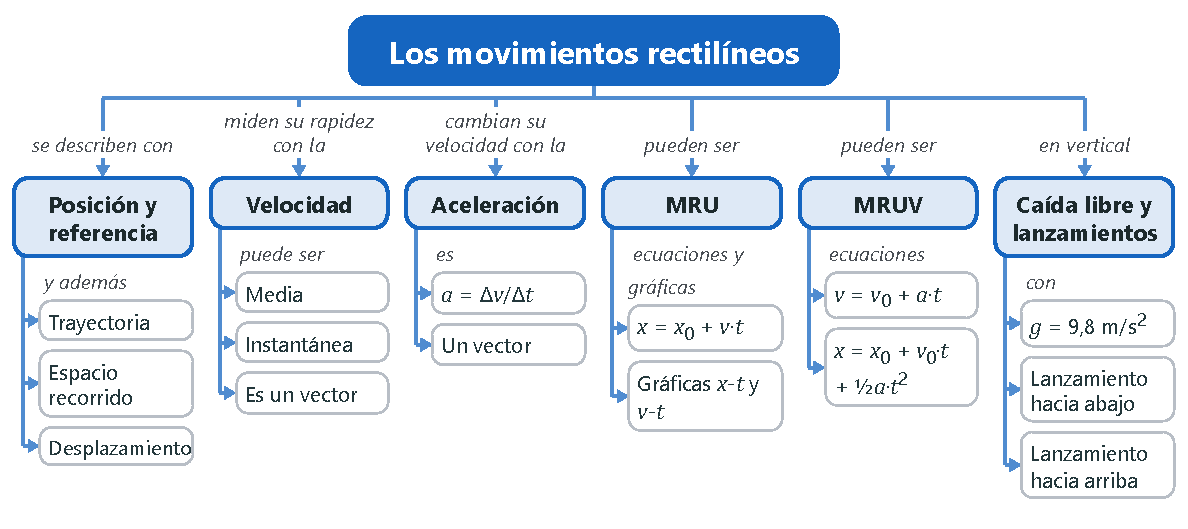
\includegraphics[width=\textwidth]{images/mapas_conceptuales/mapa_UD7}
\end{figure}

%========================================================================================
%\section*{Para empezar: batir un récord}
%\addcontentsline{toc}{section}{Para empezar: batir un récord}
%========================================================================================
%
%La experiencia dice que todos los récords acaban cayendo tarde o temprano. La superación de los deportistas y la mejora de los materiales, como las zapatillas, lo hacen posible. El 22 de julio de 2022, la estadounidense \textbf{Sydney McLaughlin} batió el récord mundial de los \qty{400}{\m} vallas con \qty{50.68}{\s}: superó diez vallas, las dos primeras con la pierna izquierda y las seis siguientes con la derecha, y mantuvo hasta el final un ritmo regular de 15 zancadas entre valla y valla. (En los Juegos de París 2024 lo rebajó todavía más, hasta \qty{50.37}{\s}.)
%
%Otro récord legendario es el de \textbf{Usain Bolt}, que en agosto de 2009 corrió los \qty{100}{\m} lisos en \qty{9.58}{\s}, una marca que nadie ha superado aún.
%
%Las hazañas de las deportistas tienen relación con el \textbf{ODS 5} (\emph{Igualdad de género}), cuya meta 5.5 busca asegurar la participación plena de las mujeres y la igualdad de oportunidades de liderazgo en todos los ámbitos. Los medios de comunicación deportivos pueden contribuir mucho a hacerlo visible.
%
%\begin{exercise}
%    ¿Qué velocidad media llevó Sydney McLaughlin en su carrera de 2022? ¿Y Usain Bolt en su récord de los \qty{100}{\m}? Expresa los resultados en \unit{\m\per\s} y en \unit{\km\per\hour}.
%    \begin{solu}
%        \textcolor{blue}{\(v_m = \dfrac{\text{espacio recorrido}}{\text{tiempo}}\); para pasar a km/h se multiplica por \num{3.6}.}
%        McLaughlin: \(v_m = \dfrac{400}{\num{50.68}} = \textcolor{red}{\qty{7.89}{\m\per\s}} = \qty{28.4}{\km\per\hour}\).
%        Bolt: \(v_m = \dfrac{100}{\num{9.58}} = \textcolor{red}{\qty{10.44}{\m\per\s}} = \qty{37.6}{\km\per\hour}\).
%    \end{solu}
%\end{exercise}
%
%\begin{exercise}
%    ¿Crees que McLaughlin mantuvo la misma velocidad durante toda la carrera? Además de la forma física, ¿pueden influir el calzado o el equipamiento en un récord?
%    \begin{solu}
%        \textcolor{red}{No}: mantuvo una cadencia regular de zancadas entre las vallas, pero la velocidad no fue constante (en la salida acelera desde el reposo y al saltar cada valla la velocidad cambia). Sí influyen el diseño y los materiales del calzado y del equipamiento (más ligeros, con mejor amortiguación y retorno de energía).
%    \end{solu}
%\end{exercise}
%
%\begin{exercise}
%    Algunos factores que influyen en una carrera son el tiempo de reacción en la salida, la capacidad de aceleración, la velocidad máxima y la capacidad de mantenerla. Debatid en clase la importancia de cada uno. ¿Qué pasos incluiríais en una agenda para alcanzar la meta 5.5 del ODS 5?
%    \begin{solu}
%        Respuesta libre.
%    \end{solu}
%\end{exercise}

%========================================================================================
\section{Posición, trayectoria y desplazamiento}
%========================================================================================

Si esperas el autobús en la parada, ves fácilmente si un coche está parado o se mueve. Pero desde dentro del autobús en marcha, ¿está en movimiento el asiento de al lado? Depende de \emph{respecto a qué} lo observes.

\subsection{Posición y sistema de referencia}

Un cuerpo en movimiento se llama \textbf{móvil}. Para describir su posición en cada instante necesitamos un \textbf{sistema de referencia}: en Física, unos ejes de coordenadas con un origen O. En el plano, la posición de un punto P queda determinada por sus coordenadas \((x, y)\).

\begin{definition}[Movimiento]
    Un cuerpo está en \textbf{movimiento} cuando su posición respecto a un sistema de referencia cambia con el tiempo. Si no cambia, está en \textbf{reposo}. El movimiento es, por tanto, \textbf{relativo}: depende del sistema de referencia elegido.
\end{definition}

\paragraph{El vector de posición.} La posición del punto P también queda determinada por el \textbf{vector de posición} \(\vec{r}\), que tiene su origen en O y su extremo en P. Su módulo es la distancia de O a P:
\[ r = \sqrt{x^2 + y^2} \]

\begin{figure}[H]
    \centering
    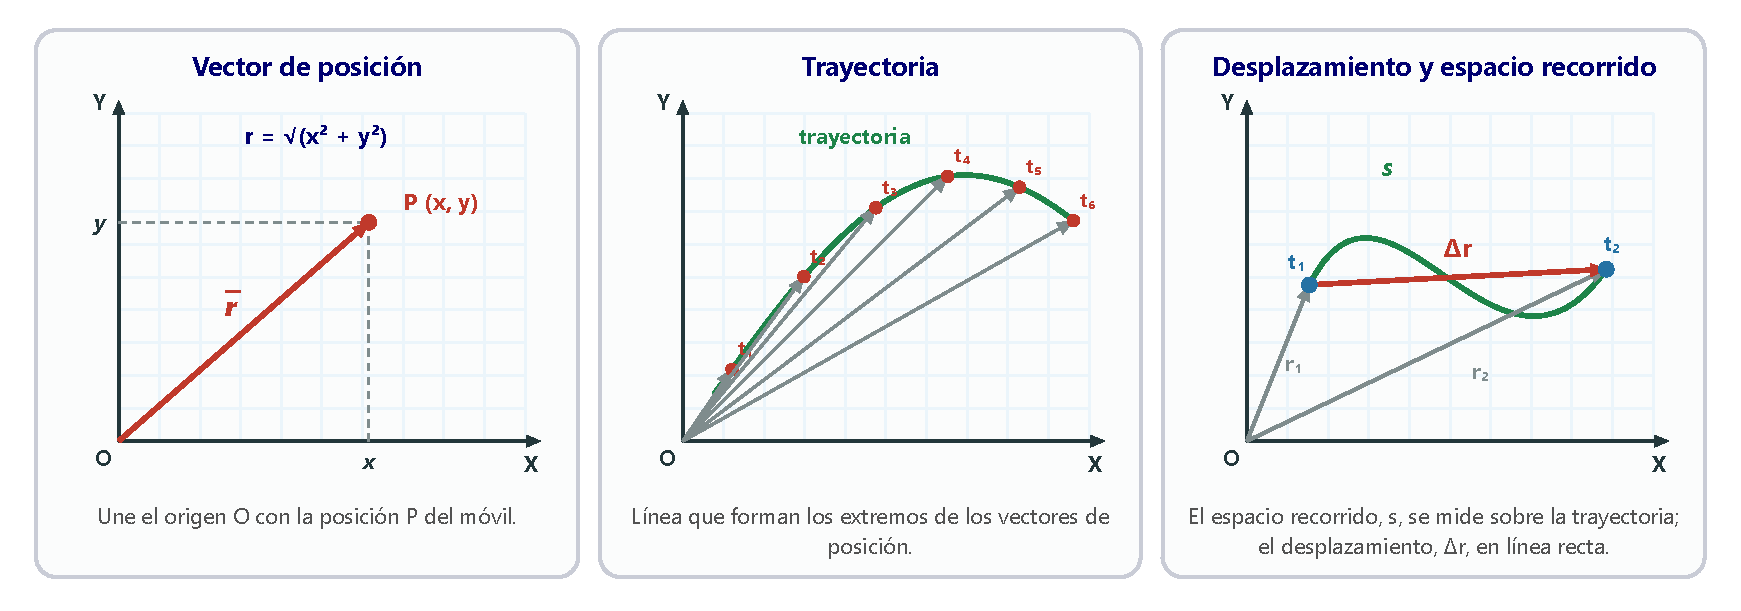
\includegraphics[width=\textwidth]{images/UD7/posicion_trayectoria}
    \caption{Vector de posición, trayectoria, desplazamiento y espacio recorrido.}
    \label{fig:posicion_trayectoria}
\end{figure}

\paragraph{Gráficas posición-tiempo.} En una gráfica posición-tiempo (\(x\)-\(t\)) se representa la posición del móvil en cada instante. En la del margen se lee que el móvil parte del origen, a los 2 s está en \(x = \qty{10}{\m}\), permanece en reposo hasta los 4 s, avanza hasta \(x = \qty{40}{\m}\) a los 6 s y vuelve al punto de partida en los 4 s siguientes.

\begin{center}
    \begin{tikzpicture}
        \begin{axis}[grafica, xlabel={\(t\) (\unit{\s})}, ylabel={\(x\) (\unit{\m})}, xmin=0, xmax=10.5, ymin=0, ymax=45, xtick={0,2,...,10}]
            \addplot coordinates {(0,0) (2,10) (4,10) (6,40) (10,0)};
        \end{axis}
    \end{tikzpicture}
\end{center}

\subsection{La trayectoria y el espacio recorrido}

\begin{definition}[Trayectoria y espacio recorrido]
    La \textbf{trayectoria} es la línea imaginaria que describe un móvil al desplazarse, formada por todas las posiciones por las que pasa. La longitud medida sobre la trayectoria es el \textbf{espacio recorrido}, \(s\), una magnitud \textbf{escalar} que se mide en metros.
\end{definition}

Según su trayectoria, los movimientos se clasifican en \textbf{rectilíneos}, si la trayectoria es una recta, y \textbf{curvilíneos}, si no lo es. Entre estos últimos están los \textbf{circulares}, los \textbf{elípticos} y los \textbf{parabólicos} (figura~\ref{fig:tipos_trayectoria}).

\begin{figure}[H]
    \centering
    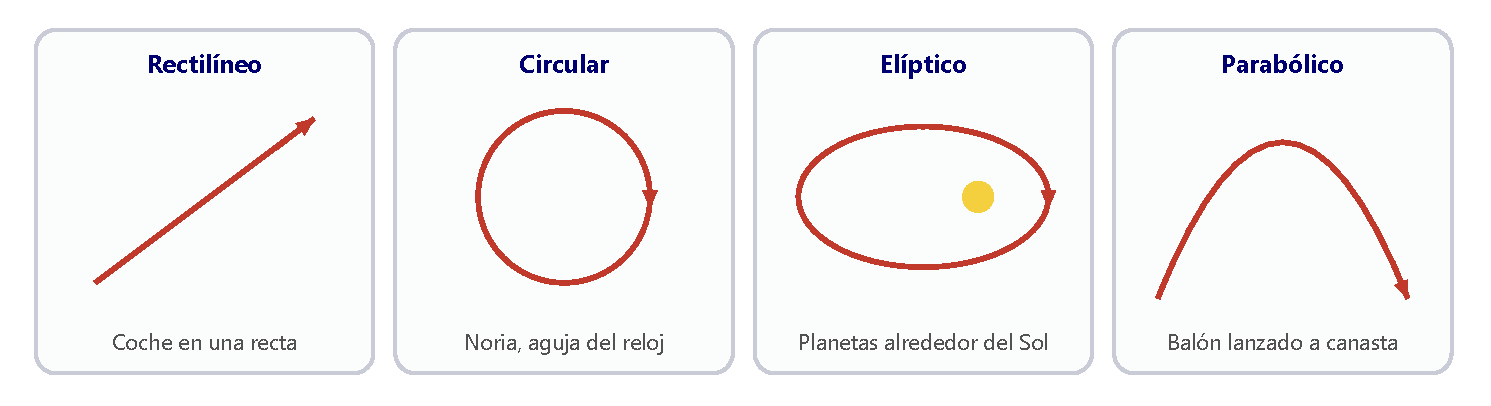
\includegraphics[width=0.95\textwidth]{images/UD7/tipos_trayectoria}
    \caption{Clasificación de los movimientos según su trayectoria.}
    \label{fig:tipos_trayectoria}
\end{figure}

\subsection{El desplazamiento}

Tres corredoras salen a la vez de la línea de salida. A los 5 segundos se han desplazado \qty{45}{\m}, \qty{35}{\m} y \qty{40}{\m}, respectivamente (figura~\ref{fig:corredoras}).

\begin{figure}[H]
    \centering
    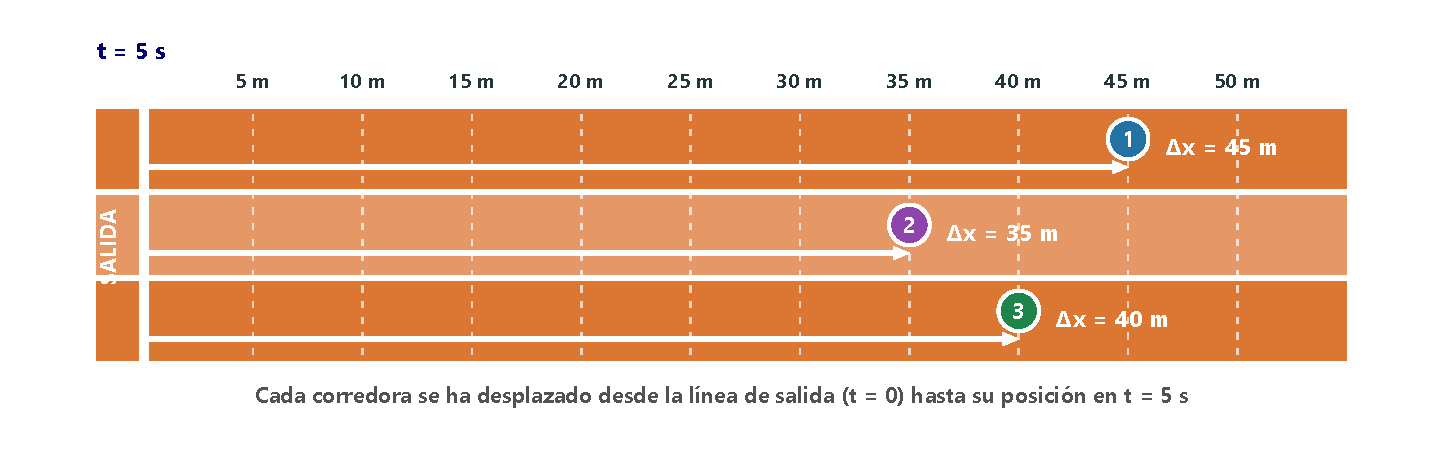
\includegraphics[width=\textwidth]{images/UD7/corredoras}
    \caption{Desplazamiento de tres corredoras al cabo de 5 segundos.}
    \label{fig:corredoras}
\end{figure}

\begin{definition}[Desplazamiento]
    El \textbf{desplazamiento} es la diferencia entre las posiciones de un móvil en dos instantes: \(\Delta x = x_2 - x_1\). Es un \textbf{vector} (\(\Delta\vec{r} = \vec{r}_2 - \vec{r}_1\)) que va de la posición inicial a la final y se mide en metros.
\end{definition}

El desplazamiento y el espacio recorrido no son lo mismo:
\begin{itemize}
    \item En un movimiento \textbf{curvilíneo}, el espacio recorrido sobre la trayectoria es mayor que el módulo del desplazamiento.
    \item En un movimiento \textbf{rectilíneo sin cambio de sentido}, ambos coinciden.
    \item Si un móvil \textbf{vuelve al punto de partida} (por ejemplo, un caballito de un tiovivo que da una vuelta completa), su desplazamiento es nulo, aunque el espacio recorrido no lo sea.
\end{itemize}

\begin{exercise}
    Dibuja un sistema de coordenadas y sitúa en él los puntos A(4, 1), B(\(-2\), 3), C(\(-3\), \(-2\)) y D(2, \(-4\)) (en metros). Dibuja sus vectores de posición y calcula sus módulos.
    \begin{solu}
        \[ r_A = \sqrt{4^2 + 1^2} = \textcolor{red}{\qty{4.12}{\m}} \qquad r_B = \sqrt{(-2)^2 + 3^2} = \textcolor{red}{\qty{3.61}{\m}} \]
        \[ r_C = \sqrt{(-3)^2 + (-2)^2} = \textcolor{red}{\qty{3.61}{\m}} \qquad r_D = \sqrt{2^2 + (-4)^2} = \textcolor{red}{\qty{4.47}{\m}} \]
    \end{solu}
\end{exercise}

\begin{exercise}
    Dibuja el vector de posición del punto (6, 8) m. ¿Cuál es su módulo?
    \begin{solu}
        \(r = \sqrt{6^2 + 8^2} = \sqrt{100} = \textcolor{red}{\qty{10}{\m}}\).
    \end{solu}
\end{exercise}

\begin{exercise}
    Representa en una gráfica posición-tiempo los datos de esta tabla y describe el movimiento:
    \begin{center}
        % --- tabla antigua ---
        % \begin{tblr}{colspec={lccccccccc}, hlines, vlines, column{1}={bg=ocre!85, fg=white, font=\bfseries}}
            % \(x\) (\unit{\m}) & 0 & 50 & 100 & 150 & 200 & 200 & 200 & 100 & 0 \\
            % \(t\) (\unit{\s}) & 0 & 5 & 10 & 15 & 20 & 25 & 30 & 35 & 40 \\
        % \end{tblr}
        % --- tabla nueva ---
        \begin{tabular}{@{}lccccccccc@{}}
            \toprule
            \textbf{\(x\) (\unit{\m})} & 0 & 50 & 100 & 150 & 200 & 200 & 200 & 100 & 0 \\[3pt]
            \textbf{\(t\) (\unit{\s})} & 0 & 5 & 10 & 15 & 20 & 25 & 30 & 35 & 40 \\
            \bottomrule
        \end{tabular}
    \end{center}
    \begin{solu}
        \begin{center}
            \begin{tikzpicture}
                \begin{axis}[grafica, xlabel={\(t\) (\unit{\s})}, ylabel={\(x\) (\unit{\m})}, xmin=0, xmax=42, ymin=0, ymax=220]
                    \addplot coordinates {(0,0) (5,50) (10,100) (15,150) (20,200) (25,200) (30,200) (35,100) (40,0)};
                \end{axis}
            \end{tikzpicture}
        \end{center}
        De 0 a 20 s el móvil se aleja del origen avanzando \qty{50}{\m} cada 5 s (\qty{10}{\m\per\s}); de 20 a 30 s está en \textcolor{red}{reposo} a \qty{200}{\m}; de 30 a 40 s \textcolor{red}{vuelve} al origen más deprisa (\qty{200}{\m} en \qty{10}{\s}, \qty{20}{\m\per\s}).
    \end{solu}
\end{exercise}

\begin{exercise}
    ¿Qué diferencia hay entre trayectoria y espacio recorrido? ¿Y entre espacio recorrido y desplazamiento?
    \begin{solu}
        La \textcolor{red}{trayectoria} es la línea que describe el móvil; el \textcolor{red}{espacio recorrido} es la longitud medida sobre esa línea. El \textcolor{red}{desplazamiento} es un vector que une la posición inicial con la final en línea recta, independientemente del camino seguido.
    \end{solu}
\end{exercise}

\begin{exercise}
    Describe la trayectoria de estos movimientos:
    \begin{enumerate}[label=\alph*)]
        \item una pelota que se deja caer;
        \item una piedra que gira atada a una cuerda;
        \item la punta del minutero de un reloj;
        \item una bolita de papel lanzada con un tirachinas;
        \item una atleta en una carrera de \qty{100}{\m} lisos;
        \item una atleta en una carrera de \qty{400}{\m}.
    \end{enumerate}
    \begin{solu}
        a) \textcolor{red}{Rectilínea} (vertical). b) y c) \textcolor{red}{Circular}. d) \textcolor{red}{Parabólica}. e) \textcolor{red}{Rectilínea}. f) \textcolor{red}{Curvilínea}: dos rectas y dos semicircunferencias.
    \end{solu}
\end{exercise}

\begin{exercise}
    Indica si son verdaderas o falsas y corrige las falsas:
    \begin{enumerate}[label=\alph*)]
        \item En una gráfica posición-tiempo se dibuja la trayectoria del móvil.
        \item Todos los movimientos curvilíneos son circulares.
        \item El desplazamiento es la trayectoria que sigue el móvil entre dos instantes.
    \end{enumerate}
    \begin{solu}
        a) \textcolor{red}{Falsa}: se representa cómo cambia la posición con el tiempo, no la forma del camino. b) \textcolor{red}{Falsa}: también hay movimientos elípticos, parabólicos\ldots{} c) \textcolor{red}{Falsa}: es la diferencia entre las posiciones final e inicial (un vector), no el camino seguido.
    \end{solu}
\end{exercise}

\begin{exercise}
    Pon dos ejemplos de movimientos rectilíneos, dos de circulares y uno de elíptico.
    \begin{solu}
        Respuesta libre. Rectilíneos: un tren en una vía recta, un objeto que cae. Circulares: una noria, un punto de un ventilador. Elíptico: la Tierra alrededor del Sol, un cometa.
    \end{solu}
\end{exercise}

\begin{exercise}
    Observa esta gráfica posición-tiempo:
    \begin{center}
        \begin{tikzpicture}
            \begin{axis}[grafica, xlabel={\(t\) (\unit{\s})}, ylabel={\(x\) (\unit{\m})}, xmin=0, xmax=10.5, ymin=0, ymax=35, xtick={0,1,...,10}]
                \addplot coordinates {(0,0) (2,10) (4,10) (6,30) (10,0)};
            \end{axis}
        \end{tikzpicture}
    \end{center}
    \begin{enumerate}[label=\alph*)]
        \item ¿Cuál ha sido el desplazamiento entre \(t = \qty{2}{\s}\) y \(t = \qty{6}{\s}\)?
        \item ¿Y el desplazamiento total?
        \item ¿Y en los cuatro últimos segundos?
        \item ¿Qué espacio total ha recorrido?
    \end{enumerate}
    \begin{solu}
        a) \(\Delta x = 30 - 10 = \textcolor{red}{\qty{20}{\m}}\). b) \(\Delta x = 0 - 0 = \textcolor{red}{0}\): vuelve al origen. c) \(\Delta x = 0 - 30 = \textcolor{red}{\qty{-30}{\m}}\) (el signo indica que se mueve hacia el origen). d) \(s = 30 + 30 = \textcolor{red}{\qty{60}{\m}}\).
    \end{solu}
\end{exercise}

\begin{exercise}
    Un móvil da una vuelta completa a una circunferencia de \qty{8}{\m} de radio. ¿Cuánto vale su desplazamiento? ¿Y el espacio recorrido?
    \begin{solu}
        El desplazamiento es \textcolor{red}{nulo}, porque vuelve al punto de partida. El espacio recorrido es la longitud de la circunferencia: \(s = 2\pi r = 2\pi \cdot 8 = \textcolor{red}{\qty{50.3}{\m}}\).
    \end{solu}
\end{exercise}

\begin{exercise}
    Calcula el espacio recorrido por un móvil que:
    \begin{enumerate}[label=\alph*)]
        \item se mueve en línea recta y sin cambiar de sentido desde \(x = \qty{-80}{\m}\) hasta \(x = \qty{520}{\m}\);
        \item da una vuelta completa a una pista circular de \qty{5}{\m} de radio.
    \end{enumerate}
    \begin{solu}
        a) \(s = 520 - (-80) = \textcolor{red}{\qty{600}{\m}}\). b) \(s = 2\pi \cdot 5 = \textcolor{red}{\qty{31.4}{\m}}\).
    \end{solu}
\end{exercise}

\begin{exercise}
    La punta del minutero de un reloj sale de las 12 y vuelve a pasar por las 12 una hora después.
    \begin{enumerate}[label=\alph*)]
        \item ¿Cómo es su trayectoria?
        \item ¿Cuál ha sido su desplazamiento?
    \end{enumerate}
    \begin{solu}
        a) \textcolor{red}{Circular}. b) \textcolor{red}{Nulo}, porque la posición final coincide con la inicial.
    \end{solu}
\end{exercise}

\begin{exercise}
    Un autobús está inicialmente a \qty{150}{\m} de una parada y se acerca a ella de forma uniforme; a los 20 s se detiene en la parada. Durante 20 s bajan los viajeros y después se aleja, de modo que 20 s más tarde está a \qty{150}{\m} de la parada. Representa la gráfica posición-tiempo tomando la parada como origen.
    \begin{solu}
        \begin{center}
            \begin{tikzpicture}
                \begin{axis}[grafica, xlabel={\(t\) (\unit{\s})}, ylabel={distancia a la parada (\unit{\m})}, xmin=0, xmax=62, ymin=0, ymax=170]
                    \addplot coordinates {(0,150) (20,0) (40,0) (60,150)};
                \end{axis}
            \end{tikzpicture}
        \end{center}
        \textcolor{blue}{Tres tramos:} se acerca (la distancia baja de 150 a 0), está parado (recta horizontal) y se aleja (la distancia sube de 0 a 150).
    \end{solu}
\end{exercise}

%========================================================================================
\section{¿Con qué rapidez cambia un móvil su posición? La velocidad}
%========================================================================================

En el ejemplo de las corredoras, la número 1 ha recorrido más distancia (\qty{45}{\m}) en el mismo tiempo (\qty{5}{\s}): es la más rápida. La magnitud que mide la rapidez con la que un cuerpo cambia de posición es la \textbf{velocidad}.

\subsection{La velocidad media}

\begin{definition}[Velocidad media]
    La \textbf{velocidad media} es el desplazamiento de un móvil dividido entre el tiempo empleado:
    \[ v_m = \frac{x - x_0}{t - t_0} = \frac{\Delta x}{\Delta t} \]
    Su unidad en el SI es el \textbf{metro por segundo} (\unit{\m\per\s}), aunque se usa mucho el \unit{\km\per\hour}.
\end{definition}

Si la trayectoria es rectilínea y el móvil no cambia de sentido, el desplazamiento coincide con el espacio recorrido y podemos escribir \(v_m = \dfrac{\Delta s}{\Delta t}\). Cuando no es así, al cociente entre el espacio recorrido y el tiempo se le llama \textbf{rapidez media}.

\begin{marker}
    \textbf{Conversión de unidades de velocidad.}
    \[ \qty{90}{\km\per\hour} = \frac{\qty{90}{\km}}{\qty{1}{\hour}} \cdot \frac{\qty{1000}{\m}}{\qty{1}{\km}} \cdot \frac{\qty{1}{\hour}}{\qty{3600}{\s}} = \qty{25}{\m\per\s} \qquad\qquad \qty{10}{\m\per\s} = \frac{\qty{10}{\m}}{\qty{1}{\s}} \cdot \frac{\qty{1}{\km}}{\qty{1000}{\m}} \cdot \frac{\qty{3600}{\s}}{\qty{1}{\hour}} = \qty{36}{\km\per\hour} \]
    Atajo: de \unit{\km\per\hour} a \unit{\m\per\s} se divide entre \num{3.6}; de \unit{\m\per\s} a \unit{\km\per\hour} se multiplica por \num{3.6}.
\end{marker}

\subsection{La velocidad instantánea}

Un ciclista recorre \qty{80}{\km} en \qty{2}{\hour}: su velocidad media es \qty{40}{\km\per\hour}. Pero seguro que en unos tramos fue más deprisa, en otros más despacio e incluso se detuvo alguna vez.

\begin{definition}[Velocidad instantánea]
    Es la velocidad de un móvil en un instante determinado o en un punto concreto de su trayectoria. Es la que marca el velocímetro de un coche.
\end{definition}

\begin{itemize}
    \item Si la velocidad instantánea es \textbf{constante} durante todo el movimiento, coincide con la media y el movimiento es \textbf{uniforme}.
    \item Si la velocidad instantánea \textbf{cambia}, el movimiento es \textbf{variado} (no uniforme).
\end{itemize}

\subsection{La velocidad es un vector}

Dos nadadoras salen a la vez del mismo punto a \qty{1.25}{\m\per\s}. ¿A qué distancia estarán a los 5 s? Si nadan en el mismo sentido, juntas; si nadan en sentidos contrarios, a \qty{12.5}{\m}. La velocidad, como el desplazamiento, es una magnitud \textbf{vectorial}: hay que indicar su módulo, su dirección y su sentido (figura~\ref{fig:velocidad_vector}).
\begin{itemize}
    \item El vector \textbf{velocidad media} tiene la dirección y el sentido del desplazamiento.
    \item El vector \textbf{velocidad instantánea} es \textbf{tangente} a la trayectoria en cada punto, apunta en el sentido del movimiento y se aplica en la posición del móvil. En un movimiento rectilíneo tiene la dirección de la propia trayectoria.
\end{itemize}

\begin{figure}[H]
    \centering
    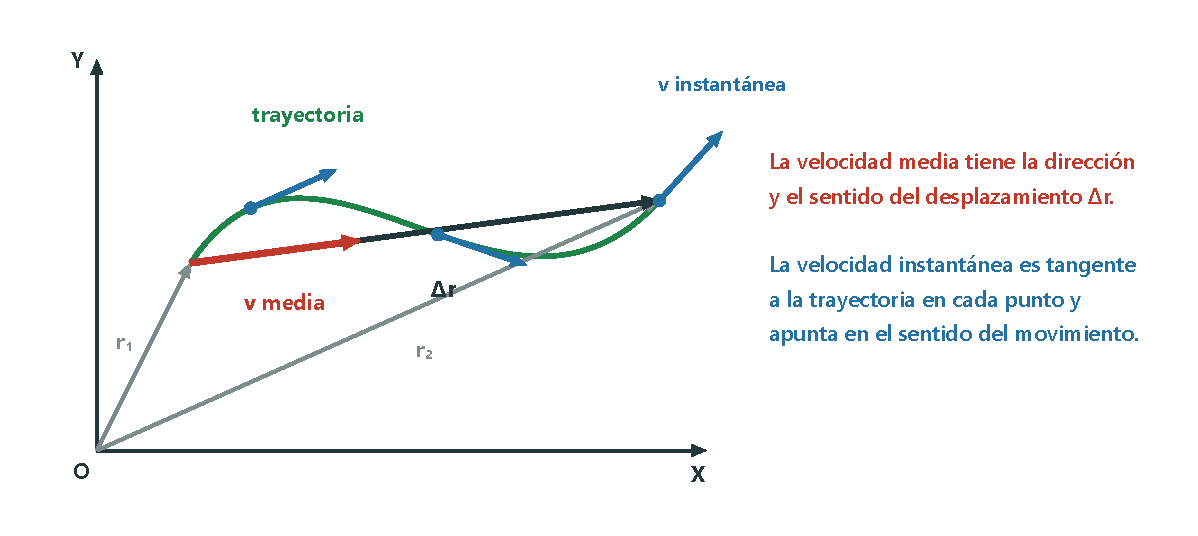
\includegraphics[width=0.85\textwidth]{images/UD7/velocidad_vector}
    \caption{Vectores velocidad media y velocidad instantánea.}
    \label{fig:velocidad_vector}
\end{figure}

\paragraph{Gráficas velocidad-tiempo.} En una gráfica \(v\)-\(t\) se lee la velocidad en cada instante. En la siguiente, el móvil parte del reposo y aumenta su velocidad hasta \qty{20}{\m\per\s} en 15 s (movimiento variado), la mantiene constante durante 15 s (movimiento uniforme) y frena hasta detenerse en 10 s (movimiento variado).

\begin{center}
    \begin{tikzpicture}
        \begin{axis}[grafica, xlabel={\(t\) (\unit{\s})}, ylabel={\(v\) (\unit{\m\per\s})}, xmin=0, xmax=42, ymin=0, ymax=24]
            \addplot coordinates {(0,0) (15,20) (30,20) (40,0)};
            \node[above] at (axis cs:15,20) {A}; \node[above] at (axis cs:30,20) {B}; \node[above right] at (axis cs:40,0) {C};
        \end{axis}
    \end{tikzpicture}
\end{center}

\begin{example}
    Una nadadora recorre una piscina de \qty{50}{\m} a \qty{1.25}{\m\per\s} constantes, descansa 30 s en el borde y vuelve al punto de salida a \qty{1}{\m\per\s}. Calcula el espacio recorrido, el desplazamiento, la rapidez media y la velocidad media en todo el recorrido.

    \textcolor{blue}{Tiempos:} \(t_1 = \dfrac{50}{\num{1.25}} = \qty{40}{\s}\); \(t_2 = \qty{30}{\s}\) (descanso); \(t_3 = \dfrac{50}{1} = \qty{50}{\s}\). Total: \qty{120}{\s}.

    \textcolor{blue}{Espacio recorrido:} \(s = 50 + 50 = \textcolor{red}{\qty{100}{\m}}\); \textcolor{blue}{rapidez media:} \(\dfrac{100}{120} = \textcolor{red}{\qty{0.83}{\m\per\s}}\).

    \textcolor{blue}{Desplazamiento:} \textcolor{red}{nulo}, porque vuelve al punto de partida; por tanto, la \textcolor{blue}{velocidad media} es \textcolor{red}{0}.
\end{example}

\begin{exercise}
    Ordena de mayor a menor estas velocidades:
    \begin{enumerate}[label=\alph*)]
        \item un caracol que recorre \qty{1}{\m} en 40 min;
        \item el sonido en el aire, \qty{340}{\m\per\s};
        \item una esquiadora que recorre \qty{6}{\km} en 20 min;
        \item la luz, \qty{3e8}{\m\per\s};
        \item un caballo que recorre \qty{15}{\km} en 30 min;
        \item un coche que recorre \qty{1.8}{\km} en 1 min.
    \end{enumerate}
    \begin{solu}
        \textcolor{blue}{Pasamos todas a m/s:} a) \(\frac{1}{2400} = \qty{4.2e-4}{\m\per\s}\); b) \qty{340}{\m\per\s}; c) \(\frac{6000}{1200} = \qty{5}{\m\per\s}\); d) \qty{3e8}{\m\per\s}; e) \(\frac{15000}{1800} = \qty{8.33}{\m\per\s}\); f) \(\frac{1800}{60} = \qty{30}{\m\per\s}\).
        \textcolor{red}{luz \(>\) sonido \(>\) coche \(>\) caballo \(>\) esquiadora \(>\) caracol}.
    \end{solu}
\end{exercise}

\begin{exercise}
    Explica la diferencia entre velocidad media y velocidad instantánea. ¿Cuándo coinciden?
    \begin{solu}
        La \textcolor{red}{media} es el desplazamiento total dividido entre el tiempo total; la \textcolor{red}{instantánea} es la velocidad en un instante concreto. Coinciden cuando el movimiento es \textcolor{red}{uniforme} (la velocidad no cambia).
    \end{solu}
\end{exercise}

\begin{exercise}
    En un campeonato, un nadador recorrió los \qty{50}{\m} libres en \qty{20.91}{\s} y los \qty{100}{\m} libres en \qty{46.40}{\s}. Calcula su velocidad media en cada prueba.
    \begin{solu}
        \(v_{50} = \frac{50}{\num{20.91}} = \textcolor{red}{\qty{2.39}{\m\per\s}}\); \quad \(v_{100} = \frac{100}{\num{46.40}} = \textcolor{red}{\qty{2.16}{\m\per\s}}\).
    \end{solu}
\end{exercise}

\begin{exercise}
    El atleta más rápido de tu clase recorre \qty{100}{\m} en \qty{15}{\s}. Calcula su velocidad media. ¿Qué distancia recorre de media cada segundo? ¿Crees que recorre realmente esa distancia en cada uno de los 15 segundos?
    \begin{solu}
        \(v_m = \frac{100}{15} = \textcolor{red}{\qty{6.67}{\m\per\s}}\): de media, \qty{6.67}{\m} cada segundo. \textcolor{red}{No}: parte del reposo, así que en los primeros segundos recorre menos y, cuando alcanza su velocidad máxima, más.
    \end{solu}
\end{exercise}

\begin{exercise}
    Halla la velocidad media de un vehículo que recorre \qty{3}{\km} en 2,5 minutos.
    \begin{solu}
        \(v_m = \frac{3000}{150} = \textcolor{red}{\qty{20}{\m\per\s}} = \qty{72}{\km\per\hour}\).
    \end{solu}
\end{exercise}

\begin{exercise}
    En 2023, el keniano Kelvin Kiptum corrió el maratón (\qty{42195}{\m}) en 2 h 0 min 35 s. ¿Cuál fue su velocidad media en \unit{\m\per\s} y en \unit{\km\per\hour}?
    \begin{solu}
        \(t = 2 \cdot 3600 + 35 = \qty{7235}{\s}\); \(v_m = \frac{42195}{7235} = \textcolor{red}{\qty{5.83}{\m\per\s}} = \textcolor{red}{\qty{21.0}{\km\per\hour}}\).
    \end{solu}
\end{exercise}

\begin{exercise}
    Halla la velocidad media de un caracol que recorre un metro en 25 minutos.
    \begin{solu}
        \(v_m = \frac{1}{1500} = \textcolor{red}{\qty{6.7e-4}{\m\per\s}}\) (unos \qty{2.4}{\m\per\hour}).
    \end{solu}
\end{exercise}

\begin{exercise}
    Luisa va en línea recta desde su casa hasta una tienda situada a \qty{300}{\m}, a \qty{1.5}{\m\per\s} constantes. Está 3 minutos en la tienda y vuelve a casa a \qty{2}{\m\per\s}.
    \begin{enumerate}[label=\alph*)]
        \item ¿Qué espacio ha recorrido?
        \item ¿Cuál ha sido su desplazamiento?
        \item ¿Cuál ha sido su rapidez media? ¿Y su velocidad media?
    \end{enumerate}
    \begin{solu}
        Tiempos: ida \(\frac{300}{\num{1.5}} = \qty{200}{\s}\); tienda \qty{180}{\s}; vuelta \(\frac{300}{2} = \qty{150}{\s}\). Total: \qty{530}{\s}.
        a) \(s = \textcolor{red}{\qty{600}{\m}}\). b) \textcolor{red}{Nulo}. c) Rapidez media: \(\frac{600}{530} = \textcolor{red}{\qty{1.13}{\m\per\s}}\); velocidad media: \textcolor{red}{0}, porque el desplazamiento es nulo.
    \end{solu}
\end{exercise}

\begin{exercise}
    Un atleta que prepara los \qty{1500}{\m} hace el recorrido en 3 min 45 s. ¿Cuál ha sido su velocidad media? ¿Crees que la ha mantenido todo el tiempo?
    \begin{solu}
        \(t = \qty{225}{\s}\); \(v_m = \frac{1500}{225} = \textcolor{red}{\qty{6.67}{\m\per\s}}\). \textcolor{red}{No}: en la salida tiene que acelerar y en el final suele cambiar de ritmo.
    \end{solu}
\end{exercise}

\begin{exercise}
    Un excursionista ve un relámpago y oye el trueno 6 s después. ¿A qué distancia está la tormenta? (Velocidad del sonido: \qty{340}{\m\per\s}; la luz llega prácticamente al instante.)
    \begin{solu}
        \(d = v \cdot t = 340 \cdot 6 = \textcolor{red}{\qty{2040}{\m}}\), unos \qty{2}{\km}.
    \end{solu}
\end{exercise}

%========================================================================================
\section{¿Cómo cambia la velocidad? La aceleración}
%========================================================================================

La velocidad de un móvil no suele ser constante: aumenta o disminuye con el tiempo.

\begin{definition}[Aceleración]
    La \textbf{aceleración} informa de cómo cambia la velocidad de un cuerpo con el tiempo. La \textbf{aceleración media} es la variación de la velocidad dividida entre el tiempo empleado:
    \[ a_m = \frac{v - v_0}{t - t_0} = \frac{\Delta v}{\Delta t} \]
    Su unidad en el SI es el \unit{\m\per\square\s} («metro por segundo al cuadrado»). La \textbf{aceleración instantánea} es la aceleración en un instante concreto.
\end{definition}

Si la aceleración instantánea es constante, coincide con la media y el movimiento es \textbf{uniformemente variado}: \textbf{acelerado} si la aceleración es positiva y \textbf{retardado} (o frenado) si es negativa. Una aceleración de \qty{2}{\m\per\square\s} significa que la velocidad aumenta \qty{2}{\m\per\s} cada segundo.

\begin{example}
    Un motorista que circula a \qty{72}{\km\per\hour} ve un obstáculo y detiene la moto en \qty{4}{\s}. ¿Cuál ha sido su aceleración? ¿Qué significa el signo?

    \textcolor{blue}{Pasamos a unidades del SI:} \(v_0 = \dfrac{72}{\num{3.6}} = \qty{20}{\m\per\s}\); \(v = 0\).
    \[ a = \frac{v - v_0}{t - t_0} = \frac{0 - 20}{4} = \textcolor{red}{\qty{-5}{\m\per\square\s}} \]
    El signo menos indica que la velocidad \textbf{disminuye}: es una aceleración de frenado.
\end{example}

\subsection{La aceleración es un vector}

Como la velocidad, la aceleración es una magnitud vectorial. En un movimiento rectilíneo:
\begin{itemize}
    \item Su \textbf{dirección} es la de la trayectoria (la misma que la del desplazamiento y la velocidad).
    \item Su \textbf{sentido} coincide con el de la velocidad si el movimiento es acelerado y es el contrario si es frenado (figura~\ref{fig:aceleracion_rampa}).
    \item Su \textbf{módulo} es \(a = \dfrac{v - v_0}{t - t_0}\).
\end{itemize}

\begin{figure}[H]
    \centering
    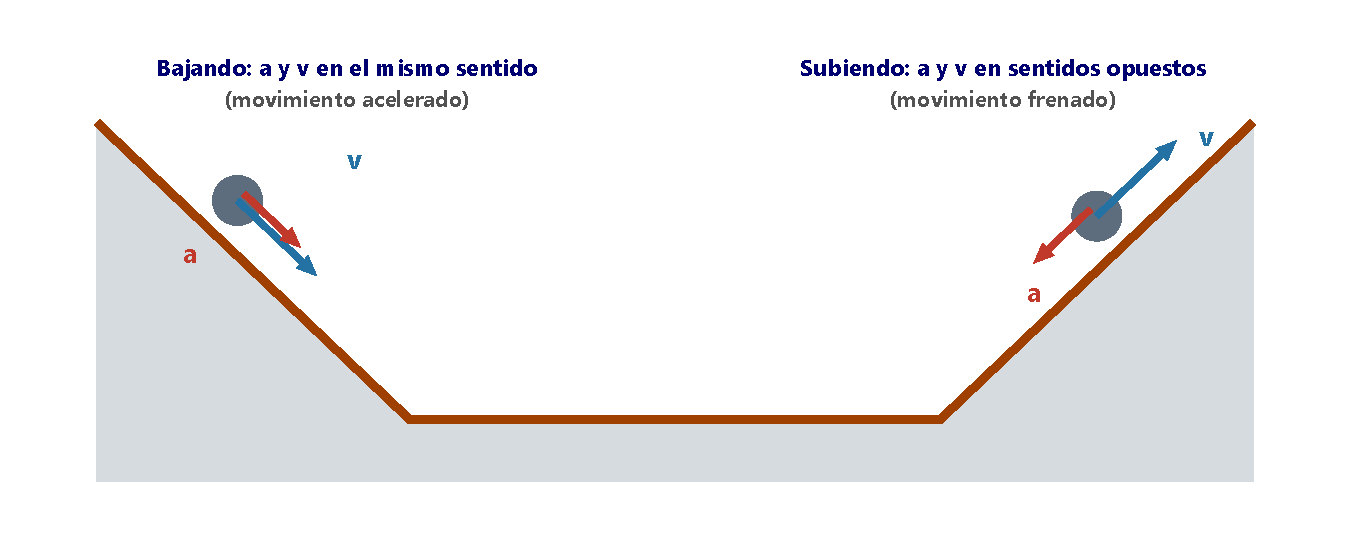
\includegraphics[width=0.9\textwidth]{images/UD7/aceleracion_rampa}
    \caption{Un monopatín en una rampa: al bajar se acelera y al subir se frena.}
    \label{fig:aceleracion_rampa}
\end{figure}

\begin{example}
    Calcula la aceleración en cada tramo de esta gráfica velocidad-tiempo:
    \begin{center}
        \begin{tikzpicture}
            \begin{axis}[grafica, xlabel={\(t\) (\unit{\s})}, ylabel={\(v\) (\unit{\m\per\s})}, xmin=0, xmax=47, ymin=0, ymax=24]
                \addplot coordinates {(0,0) (10,20) (40,20) (45,0)};
                \node[above] at (axis cs:10,20) {A}; \node[above] at (axis cs:40,20) {B}; \node[above right] at (axis cs:45,0) {C};
            \end{axis}
        \end{tikzpicture}
    \end{center}
    \textcolor{blue}{Tramo OA:} \(a = \frac{20 - 0}{10} = \textcolor{red}{\qty{2}{\m\per\square\s}}\) (acelerado). \textcolor{blue}{Tramo AB:} la velocidad no cambia: \(a = \textcolor{red}{0}\) (uniforme). \textcolor{blue}{Tramo BC:} \(a = \frac{0 - 20}{5} = \textcolor{red}{\qty{-4}{\m\per\square\s}}\) (retardado).
\end{example}

\begin{exercise}
    Explica la diferencia entre aceleración media y aceleración instantánea.
    \begin{solu}
        La \textcolor{red}{media} es la variación total de la velocidad dividida entre el tiempo total; la \textcolor{red}{instantánea}, la aceleración en un instante concreto. Coinciden si la aceleración es constante.
    \end{solu}
\end{exercise}

\begin{exercise}
    Un coche pasa de \qty{50}{\m\per\s} a \qty{65}{\m\per\s} en \qty{3}{\s}. ¿Cuál es su aceleración media?
    \begin{solu}
        \(a_m = \frac{65 - 50}{3} = \textcolor{red}{\qty{5}{\m\per\square\s}}\).
    \end{solu}
\end{exercise}

\begin{exercise}
    Un deportivo pasa de 0 a \qty{100}{\km\per\hour} en \qty{8.5}{\s}. ¿Qué aceleración media alcanza?
    \begin{solu}
        \(v = \frac{100}{\num{3.6}} = \qty{27.8}{\m\per\s}\); \(a_m = \frac{\num{27.8}}{\num{8.5}} = \textcolor{red}{\qty{3.27}{\m\per\square\s}}\).
    \end{solu}
\end{exercise}

\begin{exercise}
    El acelerador comunica a un coche una aceleración de \qty{3}{\m\per\square\s}. Si va a \qty{72}{\km\per\hour}, ¿cuánto tarda en alcanzar \qty{108}{\km\per\hour}?
    \begin{solu}
        \(v_0 = \qty{20}{\m\per\s}\); \(v = \qty{30}{\m\per\s}\); \(t = \frac{v - v_0}{a} = \frac{30 - 20}{3} = \textcolor{red}{\qty{3.3}{\s}}\).
    \end{solu}
\end{exercise}

\begin{exercise}
    Un automóvil circula a \qty{90}{\km\per\hour} y 10 s después su velocidad es \qty{108}{\km\per\hour}. ¿Cuál ha sido su aceleración?
    \begin{solu}
        \(v_0 = \qty{25}{\m\per\s}\); \(v = \qty{30}{\m\per\s}\); \(a = \frac{30 - 25}{10} = \textcolor{red}{\qty{0.5}{\m\per\square\s}}\).
    \end{solu}
\end{exercise}

\begin{exercise}
    Observa la gráfica y calcula la aceleración del móvil y su velocidad a los 8 s.
    \begin{center}
        \begin{tikzpicture}
            \begin{axis}[grafica, xlabel={\(t\) (\unit{\s})}, ylabel={\(v\) (\unit{\m\per\s})}, xmin=0, xmax=9, ymin=0, ymax=60]
                \addplot coordinates {(0,10) (2,20) (4,30) (6,40)};
            \end{axis}
        \end{tikzpicture}
    \end{center}
    \begin{solu}
        La velocidad aumenta \qty{10}{\m\per\s} cada 2 s: \(a = \frac{40 - 10}{6} = \textcolor{red}{\qty{5}{\m\per\square\s}}\). A los 8 s: \(v = 10 + 5 \cdot 8 = \textcolor{red}{\qty{50}{\m\per\s}}\).
    \end{solu}
\end{exercise}

\begin{exercise}
    Un motorista que circula a \qty{90}{\km\per\hour} ve un obstáculo y detiene la moto en \qty{5}{\s}.
    \begin{enumerate}[label=\alph*)]
        \item ¿Cuál ha sido su aceleración?
        \item ¿Qué significa el signo del resultado?
    \end{enumerate}
    \begin{solu}
        a) \(a = \frac{0 - 25}{5} = \textcolor{red}{\qty{-5}{\m\per\square\s}}\). b) Que la velocidad \textcolor{red}{disminuye}: el movimiento es frenado y la aceleración tiene sentido contrario a la velocidad.
    \end{solu}
\end{exercise}

\begin{exercise}
    Un piloto de rally necesita 4 s para detener su coche, que va a \qty{108}{\km\per\hour}. ¿Cuál es su aceleración de frenado?
    \begin{solu}
        \(a = \frac{0 - 30}{4} = \textcolor{red}{\qty{-7.5}{\m\per\square\s}}\).
    \end{solu}
\end{exercise}

\begin{exercise}
    La tabla recoge la velocidad de un vehículo que acelera de forma constante. Complétala y calcula su aceleración.
    \begin{center}
        % --- tabla antigua ---
        % \begin{tblr}{colspec={lcccccc}, hlines, vlines, column{1}={bg=ocre!85, fg=white, font=\bfseries}}
            % \(v\) (\unit{\m\per\s}) & 3 & 6 & \ldots & 12 & \ldots & 18 \\
            % \(t\) (\unit{\s}) & 1 & 2 & 3 & 4 & 5 & 6 \\
        % \end{tblr}
        % --- tabla nueva ---
        \begin{tabular}{@{}lcccccc@{}}
            \toprule
            \textbf{\(v\) (\unit{\m\per\s})} & 3 & 6 & \ldots & 12 & \ldots & 18 \\[3pt]
            \textbf{\(t\) (\unit{\s})} & 1 & 2 & 3 & 4 & 5 & 6 \\
            \bottomrule
        \end{tabular}
    \end{center}
    \begin{solu}
        La velocidad aumenta \qty{3}{\m\per\s} cada segundo: \(a = \textcolor{red}{\qty{3}{\m\per\square\s}}\). Los valores que faltan son \textcolor{red}{9} y \textcolor{red}{\qty{15}{\m\per\s}}.
    \end{solu}
\end{exercise}

%========================================================================================
\section{Movimiento rectilíneo y uniforme (MRU)}
%========================================================================================

El \textbf{movimiento rectilíneo y uniforme} (MRU) tiene:
\begin{itemize}
    \item trayectoria \textbf{rectilínea};
    \item velocidad \textbf{constante} en módulo, dirección y sentido;
    \item aceleración \textbf{nula}.
\end{itemize}

\subsection{Ecuaciones y gráficas del MRU}

La tabla recoge las posiciones de un móvil:
\begin{center}
    % --- tabla antigua ---
    % \begin{tblr}{colspec={lccccc}, hlines, vlines, column{1}={bg=ocre!85, fg=white, font=\bfseries}}
        % \(s\) (\unit{\m}) & 0 & 10 & 20 & 50 & 100 \\
        % \(t\) (\unit{\s}) & 0 & 1 & 2 & 5 & 10 \\
    % \end{tblr}
    % --- tabla nueva ---
    \begin{tabular}{@{}lccccc@{}}
        \toprule
        \textbf{\(s\) (\unit{\m})} & 0 & 10 & 20 & 50 & 100 \\[3pt]
        \textbf{\(t\) (\unit{\s})} & 0 & 1 & 2 & 5 & 10 \\
        \bottomrule
    \end{tabular}
\end{center}
Recorre espacios iguales en tiempos iguales: \qty{10}{\m} cada segundo. Su gráfica \(s\)-\(t\) es una \textbf{recta} cuya \textbf{pendiente} es la velocidad, \(v = \frac{100}{10} = \qty{10}{\m\per\s}\), y su gráfica \(v\)-\(t\) es una recta horizontal.

\begin{center}
    \begin{tikzpicture}
        \begin{axis}[grafica, width=6.5cm, xlabel={\(t\) (\unit{\s})}, ylabel={\(s\) (\unit{\m})}, xmin=0, xmax=11, ymin=0, ymax=110]
            \addplot coordinates {(0,0) (1,10) (2,20) (5,50) (10,100)};
        \end{axis}
    \end{tikzpicture}
    \qquad
    \begin{tikzpicture}
        \begin{axis}[grafica, width=6.5cm, xlabel={\(t\) (\unit{\s})}, ylabel={\(v\) (\unit{\m\per\s})}, xmin=0, xmax=11, ymin=0, ymax=12]
            \addplot[mark=none] coordinates {(0,10) (10,10)};
        \end{axis}
    \end{tikzpicture}
\end{center}

\begin{centeredequation}
    s = s_0 + v \cdot t
\end{centeredequation}
donde \(s_0\) es la posición inicial (si el móvil parte del origen, \(s = v \cdot t\)).

\begin{example}
    \textbf{Dos móviles que se cruzan.} Un coche A sale del origen a \qty{20}{\m\per\s} y, a la vez, un coche B sale de un punto situado a \qty{700}{\m} y va a su encuentro a \qty{15}{\m\per\s}. ¿Cuándo y dónde se cruzan?

    \textcolor{blue}{Ecuaciones} (tomando positivo el sentido de A): \(s_A = 20\,t\); \quad \(s_B = 700 - 15\,t\).

    \textcolor{blue}{Se cruzan cuando están en la misma posición:} \(20\,t = 700 - 15\,t \;\Rightarrow\; 35\,t = 700 \;\Rightarrow\; t = \textcolor{red}{\qty{20}{\s}}\); \(s = 20 \cdot 20 = \textcolor{red}{\qty{400}{\m}}\) del origen. A ha recorrido \qty{400}{\m} y B, \qty{300}{\m}. En la gráfica \(s\)-\(t\), el punto de corte de las dos rectas indica dónde y cuándo se cruzan:
    \begin{center}
        \begin{tikzpicture}
            \begin{axis}[grafica, xlabel={\(t\) (\unit{\s})}, ylabel={\(s\) (\unit{\m})}, xmin=0, xmax=24, ymin=0, ymax=760]
                \addplot[mark=none, color=blue!70!black] coordinates {(0,0) (24,480)}; \node[above left] at (axis cs:12,240) {A};
                \addplot[mark=none] coordinates {(0,700) (24,340)}; \node[above] at (axis cs:6,610) {B};
                \addplot[only marks, mark=*, color=black] coordinates {(20,400)};
            \end{axis}
        \end{tikzpicture}
    \end{center}
\end{example}

\begin{exercise}
    Un guepardo sigue una trayectoria rectilínea durante 8 s a \qty{108}{\km\per\hour} constantes. ¿Qué espacio recorre?
    \begin{solu}
        \(v = \qty{30}{\m\per\s}\); \(s = v \cdot t = 30 \cdot 8 = \textcolor{red}{\qty{240}{\m}}\).
    \end{solu}
\end{exercise}

\begin{exercise}
    La gráfica muestra el movimiento de dos cuerpos A y B. ¿En qué instante y en qué posición se cruzan? ¿Qué velocidad lleva cada uno?
    \begin{center}
        \begin{tikzpicture}
            \begin{axis}[grafica, xlabel={\(t\) (\unit{\s})}, ylabel={\(s\) (\unit{\m})}, xmin=0, xmax=16, ymin=0, ymax=650]
                \addplot[mark=none, color=blue!70!black] coordinates {(0,0) (15,300)}; \node[above] at (axis cs:14,280) {A};
                \addplot[mark=none] coordinates {(0,600) (15,0)}; \node[right] at (axis cs:2,520) {B};
            \end{axis}
        \end{tikzpicture}
    \end{center}
    \begin{solu}
        \(v_A = \frac{300}{15} = \textcolor{red}{\qty{20}{\m\per\s}}\); \(v_B = \frac{0 - 600}{15} = \textcolor{red}{\qty{-40}{\m\per\s}}\) (se mueve hacia el origen).
        \(20\,t = 600 - 40\,t \Rightarrow t = \textcolor{red}{\qty{10}{\s}}\), en \(s = \textcolor{red}{\qty{200}{\m}}\).
    \end{solu}
\end{exercise}

\begin{exercise}
    Dos vehículos parten a la vez del mismo punto a \qty{80}{\m\per\s} y \qty{70}{\m\per\s}. ¿Qué distancia los separa al cabo de 5 s si
    \begin{enumerate}[label=\alph*)]
        \item circulan en el mismo sentido;
        \item circulan en sentidos contrarios?
    \end{enumerate}
    \begin{solu}
        Recorren \(80 \cdot 5 = \qty{400}{\m}\) y \(70 \cdot 5 = \qty{350}{\m}\).
        a) \(400 - 350 = \textcolor{red}{\qty{50}{\m}}\). b) \(400 + 350 = \textcolor{red}{\qty{750}{\m}}\).
    \end{solu}
\end{exercise}

\begin{exercise}
    La tabla recoge las posiciones de un móvil:
    \begin{center}
        % --- tabla antigua ---
        % \begin{tblr}{colspec={lccccc}, hlines, vlines, column{1}={bg=ocre!85, fg=white, font=\bfseries}}
            % \(s\) (\unit{\m}) & 2 & 14 & 32 & 44 & 68 \\
            % \(t\) (\unit{\s}) & 0 & 2 & 5 & 7 & 11 \\
        % \end{tblr}
        % --- tabla nueva ---
        \begin{tabular}{@{}lccccc@{}}
            \toprule
            \textbf{\(s\) (\unit{\m})} & 2 & 14 & 32 & 44 & 68 \\[3pt]
            \textbf{\(t\) (\unit{\s})} & 0 & 2 & 5 & 7 & 11 \\
            \bottomrule
        \end{tabular}
    \end{center}
    \begin{enumerate}[label=\alph*)]
        \item Represéntalos y clasifica el movimiento.
        \item Halla la velocidad y escribe la ecuación del movimiento.
        \item ¿Cuánto tarda en recorrer \qty{100}{\m}?
    \end{enumerate}
    \begin{solu}
        a) Los puntos están sobre una recta: es un \textcolor{red}{MRU}.
        b) \(v = \frac{68 - 2}{11} = \textcolor{red}{\qty{6}{\m\per\s}}\); \(s = 2 + 6\,t\).
        c) \(t = \frac{100}{6} = \textcolor{red}{\qty{16.7}{\s}}\).
    \end{solu}
\end{exercise}

\begin{exercise}
    La gráfica \(v\)-\(t\) de un móvil es una recta horizontal en \(v = \qty{8}{\m\per\s}\). ¿Cuánto tarda en recorrer \qty{120}{\m}?
    \begin{solu}
        Es un MRU: \(t = \frac{s}{v} = \frac{120}{8} = \textcolor{red}{\qty{15}{\s}}\).
    \end{solu}
\end{exercise}

\begin{exercise}
    Dos coches, A y B, salen a la vez uno al encuentro del otro desde dos puntos separados \qty{2}{\km}. A va a \qty{54}{\km\per\hour} y B a \qty{90}{\km\per\hour}. ¿Cuánto tardan en encontrarse y dónde?
    \begin{solu}
        \(v_A = \qty{15}{\m\per\s}\); \(v_B = \qty{25}{\m\per\s}\). \(15\,t = 2000 - 25\,t \Rightarrow t = \textcolor{red}{\qty{50}{\s}}\); se encuentran a \(15 \cdot 50 = \textcolor{red}{\qty{750}{\m}}\) del punto de salida de A.
    \end{solu}
\end{exercise}

\begin{exercise}
    Un viajero pierde el barco, que salió hace 1 h y navega a \qty{30}{\km\per\hour}. Contrata una lancha que navega a \qty{50}{\km\per\hour}.
    \begin{enumerate}[label=\alph*)]
        \item ¿Cuánto tarda en alcanzarlo?
        \item ¿A qué distancia de la costa?
    \end{enumerate}
    \begin{solu}
        Cuando salga la lancha, el barco estará a \qty{30}{\km}. \(50\,t = 30 + 30\,t \Rightarrow t = \textcolor{red}{\qty{1.5}{\hour}}\). Distancia: \(50 \cdot \num{1.5} = \textcolor{red}{\qty{75}{\km}}\).
    \end{solu}
\end{exercise}

\begin{exercise}
    Un coche sale a las 9:00 a \qty{20}{\m\per\s}. A las 9:20 sale del mismo punto otro a \qty{30}{\m\per\s} para alcanzarlo. ¿A qué hora y a qué distancia lo alcanza?
    \begin{solu}
        En 20 min (\qty{1200}{\s}) el primero ha recorrido \(20 \cdot 1200 = \qty{24000}{\m}\). Contando el tiempo desde las 9:20: \(30\,t = 24000 + 20\,t \Rightarrow t = \qty{2400}{\s} = \qty{40}{\minute}\). Lo alcanza a las \textcolor{red}{10:00}, a \(30 \cdot 2400 = \qty{72000}{\m} = \textcolor{red}{\qty{72}{\km}}\).
    \end{solu}
\end{exercise}

%========================================================================================
\section{Movimiento rectilíneo uniformemente variado (MRUV)}
%========================================================================================

Un cuerpo describe un \textbf{movimiento rectilíneo uniformemente variado} (MRUV) si su trayectoria es rectilínea y su \textbf{aceleración es constante}. Puede ser:
\begin{itemize}
    \item \textbf{acelerado} (MRUA), si la aceleración es positiva (la velocidad aumenta);
    \item \textbf{retardado} o frenado (MRUR), si la aceleración es negativa (la velocidad disminuye).
\end{itemize}

\subsection{Ecuaciones del MRUV}

\begin{center}
    % --- tabla antigua ---
    % \begin{tblr}{colspec={lccccc}, hlines, vlines, column{1}={bg=ocre!85, fg=white, font=\bfseries}}
        % \(v\) (\unit{\m\per\s}) & 2 & 3 & 4 & 5 & 6 \\
        % \(t\) (\unit{\s}) & 0 & 1 & 2 & 3 & 4 \\
    % \end{tblr}
    % --- tabla nueva ---
    \begin{tabular}{@{}lccccc@{}}
        \toprule
        \textbf{\(v\) (\unit{\m\per\s})} & 2 & 3 & 4 & 5 & 6 \\[3pt]
        \textbf{\(t\) (\unit{\s})} & 0 & 1 & 2 & 3 & 4 \\
        \bottomrule
    \end{tabular}
    \qquad
    % --- tabla antigua ---
    % \begin{tblr}{colspec={lccccccc}, hlines, vlines, column{1}={bg=ocre!85, fg=white, font=\bfseries}}
        % \(s\) (\unit{\m}) & 0 & \num{2.5} & 6 & \num{10.5} & 16 & \num{22.5} & 30 \\
        % \(t\) (\unit{\s}) & 0 & 1 & 2 & 3 & 4 & 5 & 6 \\
    % \end{tblr}
    % --- tabla nueva ---
    \begin{tabular}{@{}lccccccc@{}}
        \toprule
        \textbf{\(s\) (\unit{\m})} & 0 & \num{2.5} & 6 & \num{10.5} & 16 & \num{22.5} & 30 \\[3pt]
        \textbf{\(t\) (\unit{\s})} & 0 & 1 & 2 & 3 & 4 & 5 & 6 \\
        \bottomrule
    \end{tabular}
\end{center}

La gráfica \(v\)-\(t\) de un MRUA es una \textbf{recta} cuya pendiente es la aceleración (aquí \(a = \qty{1}{\m\per\square\s}\)) y que corta el eje vertical en la velocidad inicial (\(v_0 = \qty{2}{\m\per\s}\)). La gráfica \(s\)-\(t\) es una \textbf{parábola}: el espacio no es proporcional al tiempo.

\begin{center}
    \begin{tikzpicture}
        \begin{axis}[grafica, width=6.5cm, xlabel={\(t\) (\unit{\s})}, ylabel={\(v\) (\unit{\m\per\s})}, xmin=0, xmax=4.5, ymin=0, ymax=7]
            \addplot coordinates {(0,2) (1,3) (2,4) (3,5) (4,6)};
        \end{axis}
    \end{tikzpicture}
    \qquad
    \begin{tikzpicture}
        \begin{axis}[grafica, width=6.5cm, xlabel={\(t\) (\unit{\s})}, ylabel={\(s\) (\unit{\m})}, xmin=0, xmax=6.5, ymin=0, ymax=32]
            \addplot[mark=none, domain=0:6, samples=40] {2*x + 0.5*x^2};
            \addplot[only marks] coordinates {(0,0) (1,2.5) (2,6) (3,10.5) (4,16) (5,22.5) (6,30)};
        \end{axis}
    \end{tikzpicture}
\end{center}

Las ecuaciones del MRUV son:
\begin{centeredequation}
    v = v_0 + a \cdot t \qquad\qquad s = s_0 + v_0 \cdot t + \frac{1}{2}\, a \cdot t^2
\end{centeredequation}
En un MRUR se usan las mismas ecuaciones, con \(a\) negativa. Si el móvil parte del reposo y del origen: \(v = a \cdot t\) y \(s = \frac{1}{2}\, a \cdot t^2\).

\begin{remark}
    \textbf{Una ecuación útil.} Despejando el tiempo de la primera ecuación y sustituyéndolo en la segunda se obtiene una relación que no depende del tiempo: \(v^2 - v_0^2 = 2\,a\,(s - s_0)\). Es muy práctica para calcular distancias de frenado.
\end{remark}

\begin{example}
    Un vehículo que circula a \qty{10}{\m\per\s} acelera durante 10 s hasta \qty{20}{\m\per\s}. Calcula su aceleración y el espacio recorrido.
    \[ a = \frac{20 - 10}{10} = \textcolor{red}{\qty{1}{\m\per\square\s}}; \qquad s = 10 \cdot 10 + \frac{1}{2} \cdot 1 \cdot 10^2 = \textcolor{red}{\qty{150}{\m}} \]
\end{example}

\begin{example}
    Un conductor que va a \qty{30}{\m\per\s} ve un desprendimiento de rocas y frena hasta detenerse en 12 s. Calcula la aceleración de frenado y el espacio que recorre hasta pararse.
    \[ 0 = 30 + a \cdot 12 \Rightarrow a = \textcolor{red}{\qty{-2.5}{\m\per\square\s}}; \qquad s = 30 \cdot 12 - \frac{1}{2} \cdot \num{2.5} \cdot 12^2 = 360 - 180 = \textcolor{red}{\qty{180}{\m}} \]
\end{example}

\begin{remark}
    \textbf{La distancia de seguridad.} Para evitar accidentes hay que guardar una \textbf{distancia de seguridad} (o de parada) con el vehículo de delante. Incluye el espacio recorrido durante el \textbf{tiempo de reacción} (lo que tardamos en pisar el freno, en el que el coche sigue a velocidad constante) y el espacio de frenado.
\end{remark}

\begin{exercise}
    El maquinista de un tren que circula a \qty{90}{\km\per\hour} ve un obstáculo en la vía a \qty{120}{\m} y frena con una aceleración de \qty{3}{\m\per\square\s}. ¿Se detendrá antes de llegar al obstáculo?
    \begin{solu}
        \(v_0 = \qty{25}{\m\per\s}\). Con \(v^2 - v_0^2 = 2\,a\,s\): \(0 - 625 = 2 \cdot (-3) \cdot s \Rightarrow s = \textcolor{red}{\qty{104.2}{\m}}\). \textcolor{red}{Sí} se detiene, a unos \qty{16}{\m} del obstáculo.
    \end{solu}
\end{exercise}

\begin{exercise}
    Describe el movimiento en cada tramo de la gráfica y calcula el espacio recorrido en el tramo AB.
    \begin{center}
        \begin{tikzpicture}
            \begin{axis}[grafica, xlabel={\(t\) (\unit{\s})}, ylabel={\(v\) (\unit{\m\per\s})}, xmin=0, xmax=32, ymin=0, ymax=45]
                \addplot coordinates {(0,0) (4,40) (30,40)};
                \node[above] at (axis cs:4,40) {A}; \node[above] at (axis cs:30,40) {B};
            \end{axis}
        \end{tikzpicture}
    \end{center}
    \begin{solu}
        Tramo OA: \textcolor{red}{MRUA}, \(a = \frac{40}{4} = \qty{10}{\m\per\square\s}\). Tramo AB: \textcolor{red}{MRU} a \qty{40}{\m\per\s}. Espacio en AB: \(s = 40 \cdot (30 - 4) = \textcolor{red}{\qty{1040}{\m}}\).
    \end{solu}
\end{exercise}

\begin{exercise}
    Un conductor que circula a \qty{72}{\km\per\hour} ve un obstáculo y frena de manera uniforme hasta detenerse en 4 s. Calcula el espacio que recorre hasta pararse:
    \begin{enumerate}[label=\alph*)]
        \item sin tener en cuenta el tiempo de reacción;
        \item si su tiempo de reacción es de 2 s.
    \end{enumerate}
    \begin{solu}
        \(v_0 = \qty{20}{\m\per\s}\); \(a = \frac{0 - 20}{4} = \qty{-5}{\m\per\square\s}\).
        a) \(s = 20 \cdot 4 - \frac{1}{2} \cdot 5 \cdot 4^2 = \textcolor{red}{\qty{40}{\m}}\).
        b) Durante la reacción recorre \(20 \cdot 2 = \qty{40}{\m}\) a velocidad constante: en total, \textcolor{red}{\qty{80}{\m}}.
    \end{solu}
\end{exercise}

\begin{exercise}
    Una ciclista que va a \qty{36}{\km\per\hour} frena con una aceleración de \qty{1}{\m\per\square\s} durante 4 s.
    \begin{enumerate}[label=\alph*)]
        \item ¿Qué velocidad lleva al cabo de los 4 s?
        \item ¿Qué espacio ha recorrido mientras frenaba?
    \end{enumerate}
    \begin{solu}
        \(v_0 = \qty{10}{\m\per\s}\); \(a = \qty{-1}{\m\per\square\s}\).
        a) \(v = 10 - 1 \cdot 4 = \textcolor{red}{\qty{6}{\m\per\s}}\). b) \(s = 10 \cdot 4 - \frac{1}{2} \cdot 1 \cdot 4^2 = \textcolor{red}{\qty{32}{\m}}\).
    \end{solu}
\end{exercise}

\begin{exercise}
    Un avión toma tierra a \qty{216}{\km\per\hour} y frena de manera uniforme usando toda la pista, de \qty{1800}{\m}.
    \begin{enumerate}[label=\alph*)]
        \item ¿Cuál es su aceleración de frenado?
        \item ¿Cuánto tarda en detenerse?
        \item ¿Qué pasaría si otro avión aterrizara a \qty{252}{\km\per\hour} con la misma aceleración?
    \end{enumerate}
    \begin{solu}
        \(v_0 = \qty{60}{\m\per\s}\).
        a) \(0 - 60^2 = 2\,a \cdot 1800 \Rightarrow a = \textcolor{red}{\qty{-1}{\m\per\square\s}}\).
        b) \(t = \frac{0 - 60}{-1} = \textcolor{red}{\qty{60}{\s}}\).
        c) Con \(v_0 = \qty{70}{\m\per\s}\): \(s = \frac{70^2}{2} = \qty{2450}{\m}\). \textcolor{red}{Necesitaría más pista} de la que hay: se saldría de ella.
    \end{solu}
\end{exercise}

\begin{exercise}
    Un vehículo parte del reposo con una aceleración de \qty{2.5}{\m\per\square\s}.
    \begin{enumerate}[label=\alph*)]
        \item ¿Qué velocidad tiene a los 8 s? ¿Qué espacio ha recorrido?
        \item Después sigue 3 minutos a esa velocidad. ¿Qué espacio recorre?
        \item Por último, frena hasta detenerse en 4 s. ¿Cuál es su aceleración de frenado y qué espacio recorre?
    \end{enumerate}
    \begin{solu}
        a) \(v = \num{2.5} \cdot 8 = \textcolor{red}{\qty{20}{\m\per\s}}\); \(s = \frac{1}{2} \cdot \num{2.5} \cdot 8^2 = \textcolor{red}{\qty{80}{\m}}\).
        b) MRU: \(s = 20 \cdot 180 = \textcolor{red}{\qty{3600}{\m}}\).
        c) \(a = \frac{0 - 20}{4} = \textcolor{red}{\qty{-5}{\m\per\square\s}}\); \(s = 20 \cdot 4 - \frac{1}{2} \cdot 5 \cdot 4^2 = \textcolor{red}{\qty{40}{\m}}\).
    \end{solu}
\end{exercise}

\begin{exercise}
    Esta gráfica corresponde a un MRUA. ¿Cuál es la velocidad inicial? ¿Y la aceleración? ¿Qué espacio recorre el móvil en el primer segundo? ¿Y en el segundo siguiente?
    \begin{center}
        \begin{tikzpicture}
            \begin{axis}[grafica, xlabel={\(t\) (\unit{\s})}, ylabel={\(v\) (\unit{\m\per\s})}, xmin=0, xmax=4.5, ymin=0, ymax=7]
                \addplot coordinates {(0,2) (4,6)};
            \end{axis}
        \end{tikzpicture}
    \end{center}
    \begin{solu}
        \(v_0 = \textcolor{red}{\qty{2}{\m\per\s}}\); \(a = \frac{6 - 2}{4} = \textcolor{red}{\qty{1}{\m\per\square\s}}\). Con \(s = 2t + \frac{1}{2}t^2\): \(s(1) = \qty{2.5}{\m}\) y \(s(2) = \qty{6}{\m}\). En el primer segundo recorre \textcolor{red}{\qty{2.5}{\m}} y en el segundo, \(6 - \num{2.5} = \textcolor{red}{\qty{3.5}{\m}}\).
    \end{solu}
\end{exercise}

\begin{exercise}
    Calcula la aceleración en cada tramo de esta gráfica:
    \begin{center}
        \begin{tikzpicture}
            \begin{axis}[grafica, xlabel={\(t\) (\unit{\s})}, ylabel={\(v\) (\unit{\m\per\s})}, xmin=0, xmax=21, ymin=0, ymax=45]
                \addplot coordinates {(0,20) (5,40) (15,40) (20,0)};
                \node[above left] at (axis cs:2.5,30) {A}; \node[above] at (axis cs:10,40) {B}; \node[right] at (axis cs:17.5,20) {C};
            \end{axis}
        \end{tikzpicture}
    \end{center}
    \begin{solu}
        A: \(a = \frac{40 - 20}{5} = \textcolor{red}{\qty{4}{\m\per\square\s}}\). B: \(a = \textcolor{red}{0}\). C: \(a = \frac{0 - 40}{5} = \textcolor{red}{\qty{-8}{\m\per\square\s}}\).
    \end{solu}
\end{exercise}

\begin{exercise}
    La conductora de un coche que va por una autopista a \qty{108}{\km\per\hour} frena y se detiene en 6 s. ¿Qué espacio recorre hasta detenerse?
    \begin{solu}
        \(a = \frac{0 - 30}{6} = \qty{-5}{\m\per\square\s}\); \(s = 30 \cdot 6 - \frac{1}{2} \cdot 5 \cdot 36 = \textcolor{red}{\qty{90}{\m}}\).
    \end{solu}
\end{exercise}

\begin{exercise}
    Un avión necesita alcanzar \qty{252}{\km\per\hour} para despegar. Si parte del reposo y tarda 50 s:
    \begin{enumerate}[label=\alph*)]
        \item ¿qué aceleración (constante) le dan los motores?
        \item ¿qué longitud mínima debe tener la pista?
    \end{enumerate}
    \begin{solu}
        \(v = \qty{70}{\m\per\s}\). a) \(a = \frac{70}{50} = \textcolor{red}{\qty{1.4}{\m\per\square\s}}\). b) \(s = \frac{1}{2} \cdot \num{1.4} \cdot 50^2 = \textcolor{red}{\qty{1750}{\m}}\).
    \end{solu}
\end{exercise}

\begin{exercise}
    Calcula la posición y la velocidad a los 4 s de estos movimientos:
    \begin{enumerate}[label=\alph*)]
        \item posición inicial \qty{20}{\m}, velocidad inicial \qty{12}{\m\per\s} y aceleración \qty{-3}{\m\per\square\s};
        \item parte del reposo desde el origen con una aceleración de \qty{3}{\m\per\square\s}.
    \end{enumerate}
    \begin{solu}
        a) \(s = 20 + 12 \cdot 4 - \frac{1}{2} \cdot 3 \cdot 16 = \textcolor{red}{\qty{44}{\m}}\); \(v = 12 - 3 \cdot 4 = \textcolor{red}{0}\) (está parado en ese instante).
        b) \(s = \frac{1}{2} \cdot 3 \cdot 16 = \textcolor{red}{\qty{24}{\m}}\); \(v = 3 \cdot 4 = \textcolor{red}{\qty{12}{\m\per\s}}\).
    \end{solu}
\end{exercise}

\begin{exercise}
    Un tren que va a \qty{54}{\km\per\hour} recorre \qty{90}{\m} desde que empieza a frenar hasta que se para. Si la aceleración es constante, calcula su valor y el tiempo de frenado.
    \begin{solu}
        \(v_0 = \qty{15}{\m\per\s}\). \(0 - 15^2 = 2\,a \cdot 90 \Rightarrow a = \textcolor{red}{\qty{-1.25}{\m\per\square\s}}\); \(t = \frac{0 - 15}{\num{-1.25}} = \textcolor{red}{\qty{12}{\s}}\).
    \end{solu}
\end{exercise}

%========================================================================================
\section{Movimientos verticales: caída libre y lanzamiento vertical}
%========================================================================================

En el siglo \textsc{xvii}, \textbf{Galileo Galilei} demostró que, si se desprecia la resistencia del aire, todos los cuerpos caen hacia la Tierra con la misma aceleración, independientemente de su masa: la \textbf{aceleración de la gravedad}, \(g = \qty{9.8}{\m\per\square\s}\).

\subsection{Caída libre}

Un cuerpo que se deja caer desde el reposo describe un \textbf{MRUA} con \(v_0 = 0\) y \(a = g\). Tomando como origen el punto desde el que cae y el sentido positivo hacia abajo:
\begin{centeredequation*}
    v = g \cdot t \qquad\qquad s = \frac{1}{2}\, g \cdot t^2
\end{centeredequation*}

\begin{example}
    La Torre de Pisa mide unos \qty{56}{\m}. ¿Cuánto tarda en llegar al suelo un objeto que se deja caer desde lo alto? ¿Con qué velocidad llega?
    \[ 56 = \frac{1}{2} \cdot \num{9.8} \cdot t^2 \Rightarrow t = \sqrt{\frac{2 \cdot 56}{\num{9.8}}} = \textcolor{red}{\qty{3.38}{\s}}; \qquad v = \num{9.8} \cdot \num{3.38} = \textcolor{red}{\qty{33.1}{\m\per\s}} \]
\end{example}

\subsection{Lanzamiento vertical hacia abajo}

Es un MRUA con velocidad inicial \(v_0\) hacia abajo y aceleración \(g\):
\begin{centeredequation*}
    v = v_0 + g \cdot t \qquad\qquad s = v_0 \cdot t + \frac{1}{2}\, g \cdot t^2
\end{centeredequation*}

\begin{example}
    Desde \qty{45}{\m} de altura se lanza un objeto hacia abajo a \qty{3}{\m\per\s}. ¿Cuánto tarda en llegar al suelo y con qué velocidad?
    \[ 45 = 3\,t + \num{4.9}\,t^2 \Rightarrow \num{4.9}\,t^2 + 3\,t - 45 = 0 \Rightarrow t = \frac{-3 + \sqrt{9 + 4 \cdot \num{4.9} \cdot 45}}{2 \cdot \num{4.9}} = \textcolor{red}{\qty{2.74}{\s}} \]
    (La otra solución es negativa y no tiene sentido físico.) \quad \(v = 3 + \num{9.8} \cdot \num{2.74} = \textcolor{red}{\qty{29.9}{\m\per\s}}\).
\end{example}

\subsection{Lanzamiento vertical hacia arriba}

Un cuerpo lanzado hacia arriba con velocidad \(v_0\) describe un \textbf{MRUR}: la gravedad tiene sentido contrario al movimiento y la velocidad disminuye hasta anularse en el punto más alto. Después el cuerpo cae en caída libre. Tomando el sentido positivo hacia arriba:
\begin{centeredequation*}
    v = v_0 - g \cdot t \qquad\qquad y = v_0 \cdot t - \frac{1}{2}\, g \cdot t^2
\end{centeredequation*}
El tiempo de subida es igual al de bajada y, en cada punto, el módulo de la velocidad es el mismo al subir y al bajar (figura~\ref{fig:lanzamiento_vertical}).

\begin{figure}[H]
    \centering
    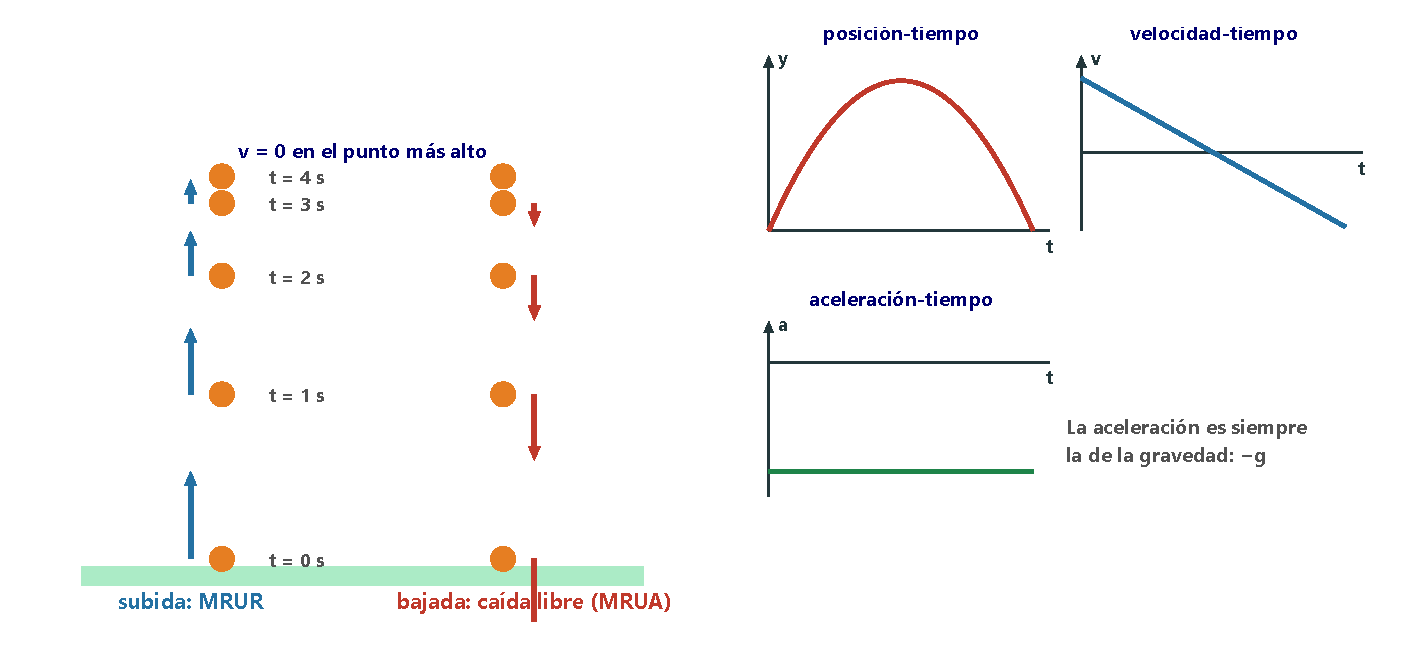
\includegraphics[width=0.95\textwidth]{images/UD7/lanzamiento_vertical}
    \caption{Lanzamiento vertical hacia arriba (\(v_0 = \qty{40}{\m\per\s}\)) y gráficas posición-tiempo, velocidad-tiempo y aceleración-tiempo.}
    \label{fig:lanzamiento_vertical}
\end{figure}

\begin{example}
    Se lanza una pelota hacia arriba a \qty{29.4}{\m\per\s}. Calcula: a) el tiempo que tarda en llegar al punto más alto; b) la altura máxima; c) cuándo pasa por \qty{40}{\m} de altura.

    a) En el punto más alto \(v = 0\): \(0 = \num{29.4} - \num{9.8}\,t \Rightarrow t = \textcolor{red}{\qty{3}{\s}}\).

    b) \(y = \num{29.4} \cdot 3 - \num{4.9} \cdot 3^2 = \textcolor{red}{\qty{44.1}{\m}}\).

    c) \(40 = \num{29.4}\,t - \num{4.9}\,t^2 \Rightarrow \num{4.9}\,t^2 - \num{29.4}\,t + 40 = 0 \Rightarrow t = \dfrac{\num{29.4} \pm \sqrt{\num{29.4}^2 - 4 \cdot \num{4.9} \cdot 40}}{2 \cdot \num{4.9}}\): \(t_1 = \textcolor{red}{\qty{2.09}{\s}}\) (al subir) y \(t_2 = \textcolor{red}{\qty{3.91}{\s}}\) (al bajar). En total tarda \qty{6}{\s} en volver al suelo.
\end{example}

\begin{exercise}
    Desde un edificio en construcción, a \qty{45}{\m} del suelo, se cae un ladrillo.
    \begin{enumerate}[label=\alph*)]
        \item ¿Cuánto tarda en llegar al suelo?
        \item ¿Con qué velocidad llega?
    \end{enumerate}
    \begin{solu}
        a) \(t = \sqrt{\frac{2 \cdot 45}{\num{9.8}}} = \textcolor{red}{\qty{3.03}{\s}}\). b) \(v = \num{9.8} \cdot \num{3.03} = \textcolor{red}{\qty{29.7}{\m\per\s}}\).
    \end{solu}
\end{exercise}

\begin{exercise}
    Desde \qty{30}{\m} de altura se lanza un objeto hacia abajo a \qty{5}{\m\per\s}. Calcula el tiempo que tarda en llegar al suelo y su velocidad en ese momento.
    \begin{solu}
        \(30 = 5\,t + \num{4.9}\,t^2 \Rightarrow t = \frac{-5 + \sqrt{25 + 588}}{\num{9.8}} = \textcolor{red}{\qty{2.02}{\s}}\); \(v = 5 + \num{9.8} \cdot \num{2.02} = \textcolor{red}{\qty{24.8}{\m\per\s}}\).
    \end{solu}
\end{exercise}

\begin{exercise}
    Un niño lanza una pelota verticalmente hacia arriba a \qty{15}{\m\per\s}. Calcula la altura máxima y el tiempo que tarda en volver a su mano.
    \begin{solu}
        Subida: \(t = \frac{15}{\num{9.8}} = \qty{1.53}{\s}\); \(y_\text{máx} = 15 \cdot \num{1.53} - \num{4.9} \cdot \num{1.53}^2 = \textcolor{red}{\qty{11.5}{\m}}\). Vuelve a la mano en \(2 \cdot \num{1.53} = \textcolor{red}{\qty{3.06}{\s}}\).
    \end{solu}
\end{exercise}

\begin{exercise}
    Se lanza un objeto hacia arriba a \qty{25}{\m\per\s}. Calcula el tiempo que tarda en alcanzar la altura máxima y el valor de esta.
    \begin{solu}
        \(t = \frac{25}{\num{9.8}} = \textcolor{red}{\qty{2.55}{\s}}\); \(y_\text{máx} = 25 \cdot \num{2.55} - \num{4.9} \cdot \num{2.55}^2 = \textcolor{red}{\qty{31.9}{\m}}\).
    \end{solu}
\end{exercise}

\begin{exercise}
    Indica si son verdaderas o falsas:
    \begin{enumerate}[label=\alph*)]
        \item si se desprecia el rozamiento con el aire, todos los cuerpos caen con la misma aceleración;
        \item en el lanzamiento hacia arriba, el tiempo de subida es mayor que el de bajada;
        \item la caída libre es un MRUR.
    \end{enumerate}
    \begin{solu}
        a) \textcolor{red}{Verdadera}. b) \textcolor{red}{Falsa}: son iguales. c) \textcolor{red}{Falsa}: es un MRUA (la velocidad aumenta).
    \end{solu}
\end{exercise}

\begin{exercise}
    Un cuerpo de \qty{5}{\kg} cae libremente desde \qty{45}{\m}.
    \begin{enumerate}[label=\alph*)]
        \item ¿Cuál es su aceleración en el primer segundo? ¿Y en el segundo?
        \item ¿Con qué velocidad llega al suelo?
    \end{enumerate}
    \begin{solu}
        a) En los dos es \(g = \textcolor{red}{\qty{9.8}{\m\per\square\s}}\): no depende de la masa ni del tiempo. b) Con \(v^2 = 2\,g\,s\): \(v = \sqrt{2 \cdot \num{9.8} \cdot 45} = \textcolor{red}{\qty{29.7}{\m\per\s}}\).
    \end{solu}
\end{exercise}

\begin{exercise}
    Un objeto que se deja caer desde una ventana tarda \qty{2.5}{\s} en llegar al suelo. ¿Desde qué altura ha caído?
    \begin{solu}
        \(s = \frac{1}{2} \cdot \num{9.8} \cdot \num{2.5}^2 = \textcolor{red}{\qty{30.6}{\m}}\).
    \end{solu}
\end{exercise}

\begin{exercise}
    Si dejamos caer un objeto desde lo alto de un edificio y medimos el espacio recorrido cada segundo, obtenemos esta tabla:
    \begin{center}
        % --- tabla antigua ---
        % \begin{tblr}{colspec={lccccccc}, hlines, vlines, column{1}={bg=ocre!85, fg=white, font=\bfseries}}
            % \(s\) (\unit{\m}) & 0 & \num{4.9} & \num{19.6} & \num{44.1} & \num{78.4} & \ldots & \ldots \\
            % \(t\) (\unit{\s}) & 0 & 1 & 2 & 3 & 4 & 5 & 6 \\
        % \end{tblr}
        % --- tabla nueva ---
        \begin{tabular}{@{}lccccccc@{}}
            \toprule
            \textbf{\(s\) (\unit{\m})} & 0 & \num{4.9} & \num{19.6} & \num{44.1} & \num{78.4} & \ldots & \ldots \\[3pt]
            \textbf{\(t\) (\unit{\s})} & 0 & 1 & 2 & 3 & 4 & 5 & 6 \\
            \bottomrule
        \end{tabular}
    \end{center}
    \begin{enumerate}[label=\alph*)]
        \item Comprueba que cumplen \(s = \frac{1}{2}\, g\, t^2\) y completa la tabla.
        \item Construye la tabla velocidad-tiempo y represéntala.
    \end{enumerate}
    \begin{solu}
        a) Por ejemplo, \(s(3) = \num{4.9} \cdot 9 = \num{44.1}\) (se cumple). Faltan \(s(5) = \textcolor{red}{\qty{122.5}{\m}}\) y \(s(6) = \textcolor{red}{\qty{176.4}{\m}}\).
        b) \(v = \num{9.8}\,t\): 0; \num{9.8}; \num{19.6}; \num{29.4}; \num{39.2}; 49; \num{58.8} \unit{\m\per\s}. La gráfica \(v\)-\(t\) es una \textcolor{red}{recta que pasa por el origen} con pendiente \(g\).
    \end{solu}
\end{exercise}

\begin{exercise}
    ¿Qué velocidad lleva un cuerpo a los 4 s de caída libre? ¿Qué espacio ha recorrido?
    \begin{solu}
        \(v = \num{9.8} \cdot 4 = \textcolor{red}{\qty{39.2}{\m\per\s}}\); \(s = \num{4.9} \cdot 16 = \textcolor{red}{\qty{78.4}{\m}}\).
    \end{solu}
\end{exercise}

\begin{exercise}
    Calcula la profundidad de un pozo si desde que soltamos una piedra hasta que oímos el golpe en el agua pasan 3 s. (Velocidad del sonido: \qty{340}{\m\per\s}.)
    \begin{solu}
        \textcolor{blue}{El tiempo total es el de caída, \(t_1\), más el que tarda el sonido en subir, \(t_2\):} \(t_1 + t_2 = 3\), con \(h = \num{4.9}\,t_1^2\) y \(h = 340\,t_2\).
        Sustituyendo: \(t_1 + \frac{\num{4.9}\,t_1^2}{340} = 3 \Rightarrow \num{0.0144}\,t_1^2 + t_1 - 3 = 0 \Rightarrow t_1 = \qty{2.88}{\s}\).
        \(h = \num{4.9} \cdot \num{2.88}^2 = \textcolor{red}{\qty{40.6}{\m}}\).
    \end{solu}
\end{exercise}


%------------------------------------------------


    \chapterimage{images/portada_cabeceras/cabecera_UD8}
    \chapter{Las fuerzas y los cambios de movimiento}

    %! Author = crist
%! Date = 25/10/2026

\spacing{1.3}
%----------------------------------------------------------------------------------------
%	UNIDAD 8: LAS FUERZAS Y LOS CAMBIOS DE MOVIMIENTO (4.º ESO)
%   Figuras: images/UD8/*.pdf (fuente HTML en images/UD8/html, SVG en images/UD8/svg)
%   Gráficas con pgfplots: estilo «grafica», definido al inicio de la UD7.
%----------------------------------------------------------------------------------------

% Mapa conceptual del tema (fuente en images/mapas_conceptuales/html/temas.js)
\begin{figure}[H]
    \centering
    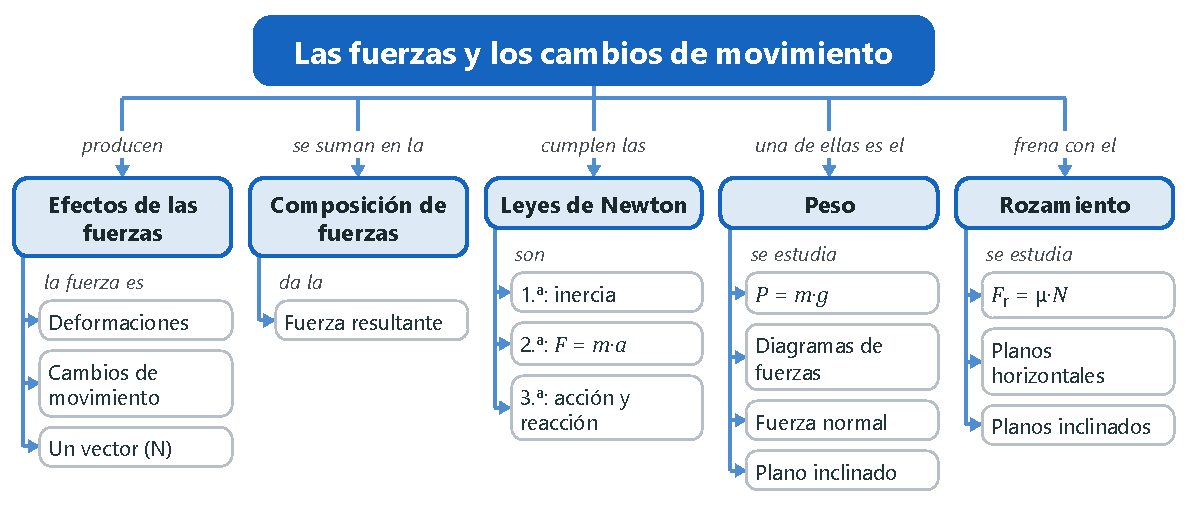
\includegraphics[width=\textwidth]{images/mapas_conceptuales/mapa_UD8}
\end{figure}

%========================================================================================
%\section*{Para empezar: aplicaciones de las leyes de la dinámica}
%\addcontentsline{toc}{section}{Para empezar: aplicaciones de las leyes de la dinámica}
%========================================================================================
%
%Si cuesta mucho poner en movimiento un cuerpo, también cuesta mucho detenerlo. Un gran petrolero cargado que navega a \qty{12}{\m\per\s} necesita \textbf{varios kilómetros} para pararse, porque tiende a mantener su estado de movimiento.
%
%En una lancha motora, la hélice empuja el agua hacia atrás y el agua, a su vez, empuja la lancha hacia delante. Mientras esa fuerza sea mayor que el rozamiento con el agua, la lancha acelera.
%
%Los fabricantes de zapatillas deportivas y de neumáticos invierten mucho dinero en diseñar productos que se agarren bien al suelo en cualquier situación. Por ejemplo, los dibujos de los neumáticos están pensados para que, cuando llueve, expulsen el agua y la rueda no pierda el contacto con el asfalto (\emph{aquaplaning}).
%
%Mejorar el agarre de los vehículos, y con ello la seguridad vial, tiene que ver con el \textbf{ODS 3} (\emph{Salud y bienestar}), cuya meta 3.6 es reducir las muertes y lesiones por accidentes de tráfico, y con el \textbf{ODS 11} (\emph{Ciudades y comunidades sostenibles}), que busca mejorar los sistemas de transporte.
%
%\begin{exercise}
%    La inercia es la tendencia de los cuerpos a mantener su estado de reposo o de movimiento. ¿Qué tiene que ver con que un petrolero necesite varios kilómetros para detenerse?
%    \begin{solu}
%        El petrolero tiene una masa enorme y, por tanto, mucha \textcolor{red}{inercia}: tiende a seguir moviéndose. Para frenarlo hace falta una fuerza que actúe durante mucho tiempo y a lo largo de mucha distancia.
%    \end{solu}
%\end{exercise}
%
%\begin{exercise}
%    Según el principio de acción y reacción, cuando dos cuerpos interaccionan, las fuerzas que se ejercen tienen igual módulo y dirección pero sentidos opuestos. ¿Cómo explica este principio el movimiento de la lancha?
%    \begin{solu}
%        La hélice empuja el agua hacia atrás (\textcolor{red}{acción}) y el agua empuja la hélice, y con ella la lancha, hacia delante (\textcolor{red}{reacción}).
%    \end{solu}
%\end{exercise}
%
%\begin{exercise}
%    ¿Para qué sirve el dibujo de la suela de las zapatillas de deporte? ¿Usarías un calzado con la suela lisa para hacer deporte? ¿Y por qué los neumáticos tienen dibujo?
%    \begin{solu}
%        El dibujo aumenta el \textcolor{red}{rozamiento} con el suelo y evita resbalar; con una suela lisa resbalaríamos con facilidad, sobre todo si el suelo está mojado. El dibujo de los neumáticos, además, \textcolor{red}{evacua el agua} cuando llueve para que la rueda siga en contacto con el asfalto.
%    \end{solu}
%\end{exercise}
%
%\begin{exercise}
%    En las carreras de coches, ¿se usan los mismos neumáticos con el asfalto seco que con el asfalto mojado? Investiga y relaciona tu respuesta con la seguridad vial y los ODS 3 y 11.
%    \begin{solu}
%        Respuesta libre. \textcolor{red}{No}: con el asfalto seco se usan neumáticos lisos (\emph{slicks}), que tienen más superficie en contacto con el suelo; con lluvia se usan neumáticos con surcos para evacuar el agua. Mejorar el agarre reduce los accidentes (ODS 3) y hace más seguro el transporte (ODS 11).
%    \end{solu}
%\end{exercise}

%========================================================================================
\section{¿Qué efectos producen las fuerzas?}
%========================================================================================

A nuestro alrededor vemos muchos efectos de las fuerzas: un muelle se estira o se encoge, un imán atrae un clavo, un balón se pone en movimiento o se detiene al golpearlo, una pelota deforma la red de la portería\ldots{} En todos los casos, la fuerza es una \textbf{interacción entre dos cuerpos}.

\begin{definition}[Fuerza]
    Una \textbf{fuerza} es toda causa capaz de modificar el estado de reposo o de movimiento de un cuerpo, o de producir en él una deformación. Su unidad en el SI es el \textbf{newton} (\unit{\newton}) y se mide con un \textbf{dinamómetro}.
\end{definition}

\subsection{La fuerza es una magnitud vectorial}

Para describir una fuerza no basta con su valor: no es lo mismo empujar una caja hacia la derecha que hacia arriba. La fuerza es un \textbf{vector} y tiene (figura~\ref{fig:vector_fuerza}):
\begin{itemize}
    \item \textbf{Punto de aplicación}: el lugar donde se aplica.
    \item \textbf{Módulo} o intensidad: su valor numérico, en newtons.
    \item \textbf{Dirección}: la de la recta sobre la que actúa.
    \item \textbf{Sentido}: el que indica la punta de la flecha.
\end{itemize}

\begin{figure}[H]
    \centering
    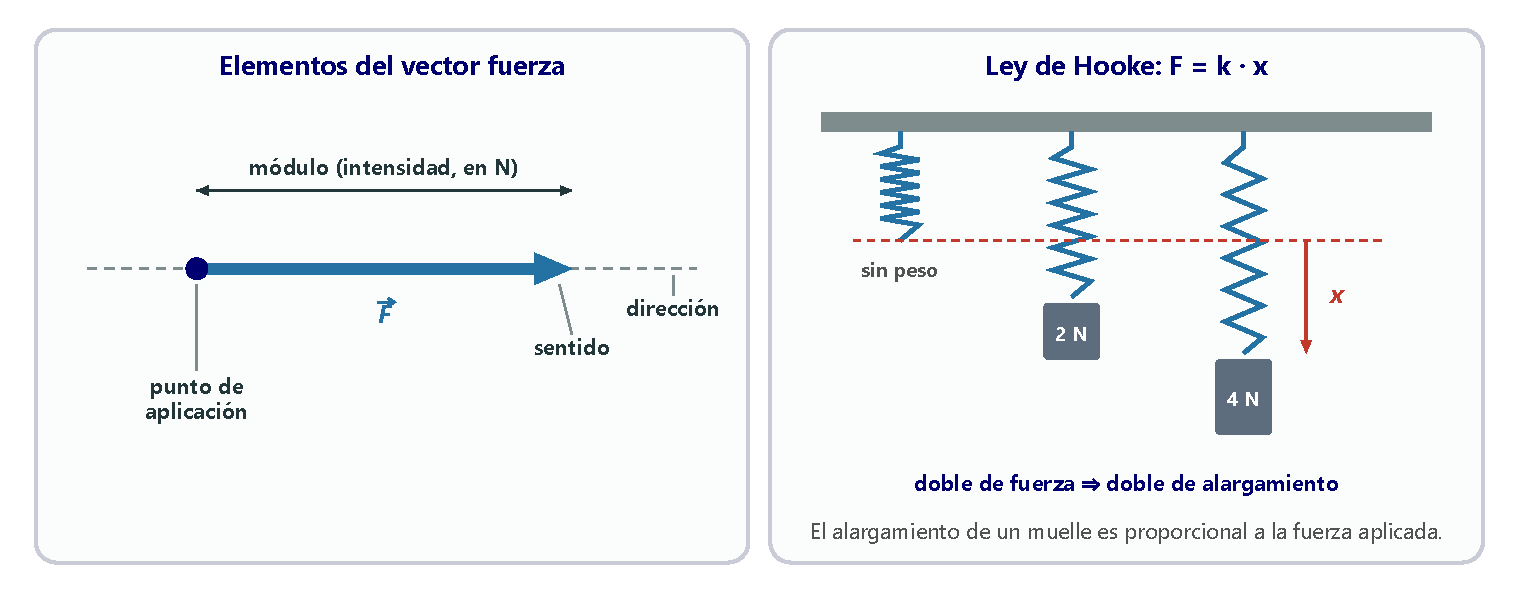
\includegraphics[width=\textwidth]{images/UD8/vector_fuerza}
    \caption{Elementos de una fuerza y ley de Hooke.}
    \label{fig:vector_fuerza}
\end{figure}

\begin{remark}
    \textbf{Ley de Hooke.} El alargamiento \(x\) que sufre un cuerpo elástico, como un muelle, es directamente proporcional a la fuerza \(F\) que lo produce: \(F = k \cdot x\). La constante \(k\), que se mide en \unit{\newton\per\m}, depende de cada muelle. En esta ley se basan los dinamómetros.
\end{remark}

\begin{exercise}
    En un partido de voleibol playa, las jugadoras golpean el balón hacia arriba; después el balón cae al otro lado de la red o, si choca con ella, la deforma. Analiza en cada situación si la fuerza cambia el estado de reposo o de movimiento del balón o produce una deformación.
    \begin{solu}
        Al golpear el balón, la fuerza \textcolor{red}{cambia su estado de movimiento} (su velocidad y su dirección) y lo \textcolor{red}{deforma} durante un instante. La gravedad cambia su movimiento haciéndolo caer. Al chocar con la red, el balón \textcolor{red}{se frena} y la red \textcolor{red}{se deforma}.
    \end{solu}
\end{exercise}

\begin{exercise}
    Cita dos ejemplos de fuerzas que deformen un cuerpo (de manera permanente o no) y dos en los que una fuerza cambie el estado de reposo o de movimiento de un cuerpo.
    \begin{solu}
        Respuesta libre. Deformaciones: estirar una goma elástica (no permanente), aplastar una lata (permanente). Cambio de movimiento: chutar un balón parado, frenar una bicicleta.
    \end{solu}
\end{exercise}

\begin{exercise}
    Un muelle se alarga \qty{4}{\cm} cuando le colgamos un peso de \qty{2}{\newton}.
    \begin{enumerate}[label=\alph*)]
        \item ¿Cuál es su constante elástica?
        \item ¿Cuánto se alargará con un peso de \qty{5}{\newton}?
    \end{enumerate}
    \begin{solu}
        a) \(k = \frac{F}{x} = \frac{2}{\num{0.04}} = \textcolor{red}{\qty{50}{\newton\per\m}}\). b) \(x = \frac{F}{k} = \frac{5}{50} = \qty{0.1}{\m} = \textcolor{red}{\qty{10}{\cm}}\).
    \end{solu}
\end{exercise}

\begin{exercise}
    Dibuja en unos ejes de coordenadas, con origen en el origen de coordenadas, una fuerza de \qty{3}{\newton} en el sentido positivo del eje X y otra de \qty{5}{\newton} en el sentido negativo del eje Y. Dibuja también las fuerzas opuestas a ellas y describe sus elementos.
    \begin{solu}
        Las cuatro tienen el punto de aplicación en O. \(\vec{F}_1\): módulo \qty{3}{\newton}, dirección del eje X, sentido positivo. \(\vec{F}_2\): módulo \qty{5}{\newton}, dirección del eje Y, sentido negativo. Sus opuestas tienen el \textcolor{red}{mismo módulo y dirección} pero \textcolor{red}{sentido contrario}: \qty{3}{\newton} hacia el X negativo y \qty{5}{\newton} hacia el Y positivo.
    \end{solu}
\end{exercise}

%========================================================================================
\section{¿Qué ocurre cuando actúan varias fuerzas? Composición de fuerzas}
%========================================================================================

Cuando varias fuerzas actúan a la vez sobre un cuerpo forman un \textbf{sistema de fuerzas}. Se llama \textbf{fuerza resultante}, \(\vec{R}\), a la fuerza que produce por sí sola el mismo efecto que todas ellas juntas.

\begin{definition}[Equilibrio]
    Un cuerpo está en \textbf{equilibrio} cuando está en reposo o se mueve con MRU. Para ello, la \textbf{resultante} de todas las fuerzas que actúan sobre él debe ser \textbf{nula}.
\end{definition}

\begin{figure}[H]
    \centering
    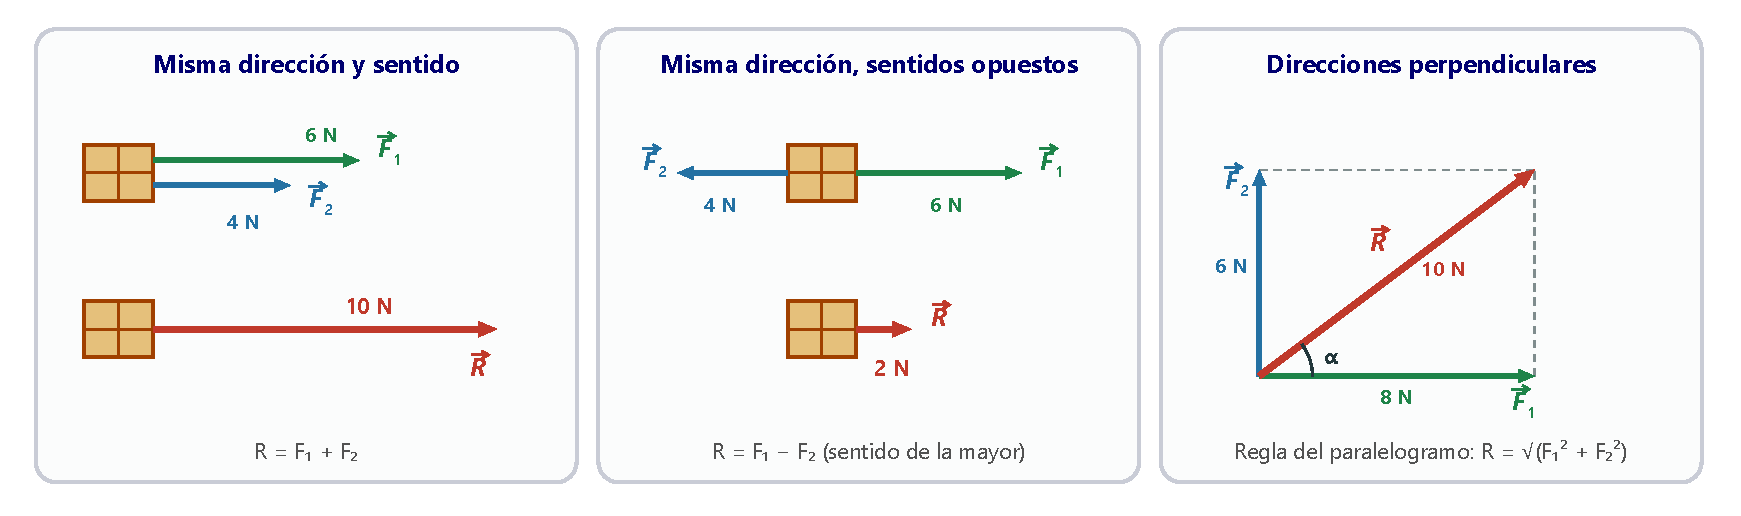
\includegraphics[width=\textwidth]{images/UD8/composicion_fuerzas}
    \caption{Resultante de dos fuerzas en tres casos.}
    \label{fig:composicion_fuerzas}
\end{figure}

\begin{itemize}
    \item \textbf{Misma dirección y sentido.} La resultante tiene la misma dirección y sentido, y su módulo es la \textbf{suma}: \(R = F_1 + F_2\).
    \item \textbf{Misma dirección y sentidos opuestos.} La resultante tiene la misma dirección, el sentido de la fuerza mayor y su módulo es la \textbf{diferencia}: \(R = F_1 - F_2\).
    \item \textbf{Direcciones perpendiculares.} Se aplica la \textbf{regla del paralelogramo}: se trazan por el extremo de cada fuerza paralelas a la otra; la resultante es la diagonal del paralelogramo. Su módulo se calcula con el teorema de Pitágoras y el ángulo con el eje X, con la trigonometría:
    \[ R = \sqrt{F_1^2 + F_2^2} \qquad \cos\alpha = \frac{F_1}{R} \qquad \sin\alpha = \frac{F_2}{R} \]
\end{itemize}

Para que un cuerpo sobre el que actúa una resultante \(\vec{R}\) quede en equilibrio hay que aplicarle otra fuerza, la \textbf{equilibrante}, del mismo módulo y dirección pero de sentido contrario.

\begin{example}
    Calcula la resultante de dos fuerzas perpendiculares de \qty{8}{\newton} (eje X) y \qty{6}{\newton} (eje Y) aplicadas en el mismo punto y el ángulo que forma con el eje X.
    \[ R = \sqrt{8^2 + 6^2} = \sqrt{100} = \textcolor{red}{\qty{10}{\newton}}; \qquad \cos\alpha = \frac{8}{10} = \num{0.8} \;\Rightarrow\; \alpha = \textcolor{red}{\ang{36.87}} \]
\end{example}

\begin{exercise}
    Dos fuerzas de la misma dirección y sentido, de \qty{12}{\newton} y \qty{9}{\newton}, actúan sobre un cuerpo.
    \begin{enumerate}[label=\alph*)]
        \item Calcula la resultante.
        \item ¿Qué fuerza habría que aplicar para equilibrarlas?
    \end{enumerate}
    \begin{solu}
        a) \(R = 12 + 9 = \textcolor{red}{\qty{21}{\newton}}\), con la misma dirección y sentido. b) Una fuerza de \textcolor{red}{\qty{21}{\newton}} con la misma dirección y \textcolor{red}{sentido contrario}.
    \end{solu}
\end{exercise}

\begin{exercise}
    Calcula la resultante de dos fuerzas de \qty{5}{\newton} y \qty{2}{\newton} con la misma dirección y sentidos contrarios.
    \begin{solu}
        \(R = 5 - 2 = \textcolor{red}{\qty{3}{\newton}}\), con la dirección común y el sentido de la fuerza de \qty{5}{\newton}.
    \end{solu}
\end{exercise}

\begin{exercise}
    Determina gráfica y numéricamente la resultante de dos fuerzas perpendiculares de \qty{60}{\newton} cada una. ¿Qué ángulo forma con el eje X?
    \begin{solu}
        \(R = \sqrt{60^2 + 60^2} = \textcolor{red}{\qty{84.9}{\newton}}\); \(\cos\alpha = \frac{60}{\num{84.9}} = \num{0.707} \Rightarrow \alpha = \textcolor{red}{\ang{45}}\): es la diagonal de un cuadrado.
    \end{solu}
\end{exercise}

\begin{exercise}
    Determina la resultante de dos fuerzas perpendiculares de \qty{12}{\newton} (eje X) y \qty{9}{\newton} (eje Y) y el ángulo que forma con el eje X.
    \begin{solu}
        \(R = \sqrt{144 + 81} = \textcolor{red}{\qty{15}{\newton}}\); \(\cos\alpha = \frac{12}{15} = \num{0.8} \Rightarrow \alpha = \textcolor{red}{\ang{36.87}}\).
    \end{solu}
\end{exercise}

\begin{exercise}
    Una fuerza de \qty{100}{\newton} es la resultante de dos fuerzas perpendiculares, una de las cuales vale \qty{60}{\newton}. ¿Cuánto vale la otra?
    \begin{solu}
        \(R^2 = F_1^2 + F_2^2 \Rightarrow F_2 = \sqrt{100^2 - 60^2} = \sqrt{6400} = \textcolor{red}{\qty{80}{\newton}}\).
    \end{solu}
\end{exercise}

\begin{exercise}
    Un remero empuja una barca río arriba con una fuerza de \qty{750}{\newton}, y la corriente la empuja río abajo con \qty{300}{\newton}. ¿Cuál es la resultante?
    \begin{solu}
        \(R = 750 - 300 = \textcolor{red}{\qty{450}{\newton}}\), \textcolor{red}{río arriba}.
    \end{solu}
\end{exercise}

\begin{exercise}
    Dos fuerzas de \qty{15}{\newton} y \qty{7}{\newton} aplicadas en un mismo cuerpo y con la misma dirección dan unas veces una resultante de \qty{22}{\newton} y otras de \qty{8}{\newton}. ¿A qué se debe?
    \begin{solu}
        Si tienen el \textcolor{red}{mismo sentido}, se suman: \(15 + 7 = \qty{22}{\newton}\). Si tienen \textcolor{red}{sentidos opuestos}, se restan: \(15 - 7 = \qty{8}{\newton}\).
    \end{solu}
\end{exercise}

\begin{exercise}
    Dos fuerzas de \qty{4}{\newton} y \qty{8}{\newton} están aplicadas en el mismo punto. Calcula la resultante si:
    \begin{enumerate}[label=\alph*)]
        \item tienen la misma dirección y sentido;
        \item tienen la misma dirección y sentidos opuestos;
        \item son perpendiculares.
    \end{enumerate}
    ¿Qué fuerza equilibraría cada resultante?
    \begin{solu}
        a) \(R = \textcolor{red}{\qty{12}{\newton}}\). b) \(R = \textcolor{red}{\qty{4}{\newton}}\) en el sentido de la de \qty{8}{\newton}. c) \(R = \sqrt{16 + 64} = \textcolor{red}{\qty{8.94}{\newton}}\), que forma con la fuerza de \qty{8}{\newton} un ángulo de \ang{26.6} (\(\cos\alpha = \frac{8}{\num{8.94}}\)). En cada caso, la equilibrante es una fuerza del mismo módulo y dirección que la resultante y sentido contrario.
    \end{solu}
\end{exercise}

\begin{exercise}
    Calcula la resultante de dos fuerzas perpendiculares de \qty{8}{\newton} y \qty{15}{\newton} aplicadas a un cuerpo.
    \begin{solu}
        \(R = \sqrt{64 + 225} = \sqrt{289} = \textcolor{red}{\qty{17}{\newton}}\).
    \end{solu}
\end{exercise}

%========================================================================================
\section{Fuerzas y cambios de movimiento: las leyes de Newton}
%========================================================================================

La parte de la Física que estudia la relación entre las fuerzas y los cambios de movimiento se llama \textbf{dinámica}. Sus fundamentos son las tres leyes que publicó Isaac \textbf{Newton} en 1687.

\subsection{La primera ley de Newton o principio de inercia}

¿Si un cuerpo está en reposo, es que no actúa ninguna fuerza sobre él? No necesariamente: un bloque sobre el que tiran dos fuerzas iguales y opuestas sigue en reposo, porque la resultante es nula. ¿Y hace falta una fuerza para que un cuerpo siga moviéndose? Una bola que rueda por una superficie horizontal perfectamente lisa no cambiaría su velocidad ni su dirección, aunque no la empujara nadie. En cambio, en un plano inclinado, la bola acelera al bajar y se frena al subir, porque el peso actúa sobre ella.

\begin{definition}[Primera ley de Newton o principio de inercia]
    Si sobre un cuerpo no actúa ninguna fuerza neta, el cuerpo permanece en \textbf{reposo} o se mueve con \textbf{movimiento rectilíneo y uniforme}. La \textbf{inercia} es la tendencia de los cuerpos a mantener su estado de reposo o de movimiento.
\end{definition}

Según el principio de inercia, el reposo y el MRU son equivalentes. Si un cuerpo acelera, frena o cambia de dirección, es que sobre él actúa una fuerza neta.

\begin{exercise}
    Indica si son verdaderas o falsas:
    \begin{enumerate}[label=\alph*)]
        \item si actúa una fuerza sobre un cuerpo, este tiene que cambiar su estado de reposo o de MRU;
        \item si no actúa ninguna fuerza sobre un cuerpo, este se mantiene en reposo o con MRU.
    \end{enumerate}
    \begin{solu}
        a) \textcolor{red}{Falsa}: si actúan varias fuerzas cuya resultante es nula, el estado no cambia. Lo correcto es decir «si actúa una fuerza \emph{neta}». b) \textcolor{red}{Verdadera}: es el principio de inercia.
    \end{solu}
\end{exercise}

\begin{exercise}
    Tapa un vaso con un naipe y pon una moneda encima. Si golpeas el naipe con fuerza en horizontal, ¿dónde cae la moneda? Justifícalo.
    \begin{solu}
        La moneda cae \textcolor{red}{dentro del vaso}. Por la \textcolor{red}{inercia}, tiende a seguir en reposo: el naipe sale disparado sin apenas arrastrarla, y la moneda, al quedarse sin apoyo, cae.
    \end{solu}
\end{exercise}

\begin{exercise}
    Cuando un coche frena bruscamente, los pasajeros siguen moviéndose hacia delante por la inercia; el cinturón de seguridad lo impide.
    \begin{enumerate}[label=\alph*)]
        \item ¿Para qué sirve el reposacabezas?
        \item ¿Por qué sientes que te empujan hacia atrás cuando el coche arranca bruscamente?
    \end{enumerate}
    \begin{solu}
        a) Si el coche recibe un golpe por detrás y acelera bruscamente, la cabeza tiende a quedarse donde estaba (inercia) y se iría hacia atrás: el reposacabezas la sujeta y evita lesiones en el cuello. b) Porque tu cuerpo tiende a seguir en reposo mientras el asiento avanza: en realidad no hay ninguna fuerza que te empuje hacia atrás, es el asiento el que te empuja hacia delante.
    \end{solu}
\end{exercise}

\begin{exercise}
    ¿Qué fuerza neta actúa sobre un coche que circula en línea recta a \qty{100}{\km\per\hour} constantes?
    \begin{solu}
        \textcolor{red}{Ninguna}: si se mueve con MRU, la fuerza neta es \textcolor{red}{nula}. La fuerza del motor compensa exactamente los rozamientos.
    \end{solu}
\end{exercise}

\subsection{La segunda ley de Newton o principio fundamental de la dinámica}

Si sobre un cuerpo actúa una fuerza neta, el cuerpo adquiere una aceleración. Para estudiarlo, colocamos un carrito en un carril, tiramos de él con distintas fuerzas (poniendo pesas en un portapesas) y medimos su aceleración a partir del tiempo que tarda en recorrer una distancia (\(a = 2s/t^2\)):

\begin{center}
    % --- tabla antigua ---
    % \begin{tblr}{colspec={lccccc}, hlines, vlines, column{1}={bg=ocre!85, fg=white, font=\bfseries}}
        % \(F\) (\unit{\newton}) & 2 & 3 & 4 & 5 & 6 \\
        % \(a\) (\unit{\m\per\square\s}) & \num{1.0} & \num{1.5} & \num{2.0} & \num{2.5} & \num{3.0} \\
    % \end{tblr}
    % --- tabla nueva ---
    \begin{tabular}{@{}lccccc@{}}
        \toprule
        \textbf{\(F\) (\unit{\newton})} & 2 & 3 & 4 & 5 & 6 \\[3pt]
        \textbf{\(a\) (\unit{\m\per\square\s})} & \num{1.0} & \num{1.5} & \num{2.0} & \num{2.5} & \num{3.0} \\
        \bottomrule
    \end{tabular}
    \qquad
    \begin{tikzpicture}[baseline=(current bounding box.center)]
        \begin{axis}[grafica, width=6cm, height=4.5cm, xlabel={\(a\) (\unit{\m\per\square\s})}, ylabel={\(F\) (\unit{\newton})}, xmin=0, xmax=3.3, ymin=0, ymax=7]
            \addplot coordinates {(1,2) (1.5,3) (2,4) (2.5,5) (3,6)};
            \addplot[mark=none, dashed, line width=0.8pt] coordinates {(0,0) (1,2)};
        \end{axis}
    \end{tikzpicture}
\end{center}

El cociente \(F/a\) es siempre el mismo, \qty{2}{\kg}: es la \textbf{masa} del carrito, que mide su \textbf{inercia}, es decir, lo que cuesta cambiar su estado de movimiento.

\begin{definition}[Segunda ley de Newton]
    La aceleración de un cuerpo es directamente proporcional a la fuerza neta que actúa sobre él, tiene su misma dirección y sentido, y es inversamente proporcional a su masa:
    \[ \vec{F}_\text{neta} = m \cdot \vec{a} \]
    Un \textbf{newton} es la fuerza que comunica a \qty{1}{\kg} de masa una aceleración de \qty{1}{\m\per\square\s}: \(\qty{1}{\newton} = \qty{1}{\kg\cdot\m\per\square\s}\).
\end{definition}

\begin{itemize}
    \item Si \(F_\text{neta} = 0\), la aceleración es nula: el cuerpo está en reposo o con MRU (primera ley).
    \item Si la fuerza neta tiene el sentido del movimiento, el cuerpo describe un \textbf{MRUA}.
    \item Si tiene sentido contrario al movimiento, el cuerpo describe un \textbf{MRUR} hasta pararse.
    \item Si es perpendicular al movimiento, el cuerpo \textbf{cambia de dirección}.
\end{itemize}

\begin{example}
    ¿Qué fuerza horizontal hay que aplicar a un cuerpo de \qty{40}{\kg} en reposo sobre un plano horizontal sin rozamiento para que alcance \qty{54}{\km\per\hour} en 6 s?

    \textcolor{blue}{Aceleración (MRUA):} \(v = \qty{15}{\m\per\s}\); \(a = \dfrac{15 - 0}{6} = \qty{2.5}{\m\per\square\s}\).

    \textcolor{blue}{Segunda ley:} \(F = m \cdot a = 40 \cdot \num{2.5} = \textcolor{red}{\qty{100}{\newton}}\).
\end{example}

\begin{exercise}
    ¿Qué fuerza hay que aplicar al carrito del experimento (\(m = \qty{2}{\kg}\)) para que adquiera una aceleración de \qty{1.5}{\m\per\square\s}? ¿Y de \qty{2.5}{\m\per\square\s}?
    \begin{solu}
        \(F = 2 \cdot \num{1.5} = \textcolor{red}{\qty{3}{\newton}}\); \(F = 2 \cdot \num{2.5} = \textcolor{red}{\qty{5}{\newton}}\).
    \end{solu}
\end{exercise}

\begin{exercise}
    ¿Qué fuerza hay que aplicar a un cuerpo de masa \(2m\) para que tenga la misma aceleración que otro de masa \(m\) al que se aplica una fuerza \(F\)? ¿Y si además queremos que la aceleración sea el doble?
    \begin{solu}
        Con la misma aceleración: \(F' = 2m \cdot a = \textcolor{red}{2F}\). Con el doble de aceleración: \(F'' = 2m \cdot 2a = \textcolor{red}{4F}\).
    \end{solu}
\end{exercise}

\begin{exercise}
    Una misma fuerza aplicada a dos cuerpos produce en uno una aceleración de \qty{1.8}{\m\per\square\s} y en el otro de \qty{9}{\m\per\square\s}. ¿Qué relación hay entre sus masas?
    \begin{solu}
        \(m_1 \cdot \num{1.8} = m_2 \cdot 9 \Rightarrow \frac{m_1}{m_2} = \frac{9}{\num{1.8}} = \textcolor{red}{5}\): el primero tiene \textcolor{red}{5 veces más masa}.
    \end{solu}
\end{exercise}

\begin{exercise}
    Un coche de \qty{1200}{\kg} parte del reposo empujado por una fuerza neta de \qty{2400}{\newton} en una carretera recta y horizontal. ¿Qué velocidad tendrá a los 10 s? ¿Qué espacio habrá recorrido?
    \begin{solu}
        \(a = \frac{2400}{1200} = \qty{2}{\m\per\square\s}\); \(v = 2 \cdot 10 = \textcolor{red}{\qty{20}{\m\per\s}}\); \(s = \frac{1}{2} \cdot 2 \cdot 10^2 = \textcolor{red}{\qty{100}{\m}}\).
    \end{solu}
\end{exercise}

\begin{exercise}
    Un coche de \qty{1200}{\kg} circula a \qty{72}{\km\per\hour}. ¿Qué fuerza deben ejercer los frenos para detenerlo en \qty{80}{\m}?
    \begin{solu}
        \(v_0 = \qty{20}{\m\per\s}\). \(0 - 20^2 = 2\,a \cdot 80 \Rightarrow a = \qty{-2.5}{\m\per\square\s}\); \(F = 1200 \cdot \num{2.5} = \textcolor{red}{\qty{3000}{\newton}}\), en sentido contrario al movimiento.
    \end{solu}
\end{exercise}

\begin{exercise}
    Un camión de 15 toneladas pasa de \qty{54}{\km\per\hour} a \qty{90}{\km\per\hour} en 50 s por una carretera horizontal. Calcula la fuerza neta, supuesta constante.
    \begin{solu}
        \(a = \frac{25 - 15}{50} = \qty{0.2}{\m\per\square\s}\); \(F = 15000 \cdot \num{0.2} = \textcolor{red}{\qty{3000}{\newton}}\).
    \end{solu}
\end{exercise}

\begin{exercise}
    ¿Qué fuerza horizontal constante hay que aplicar a un cuerpo de \qty{4}{\kg} en reposo sobre un plano horizontal sin rozamiento para que alcance \qty{18}{\km\per\hour} en 2 s?
    \begin{solu}
        \(a = \frac{5}{2} = \qty{2.5}{\m\per\square\s}\); \(F = 4 \cdot \num{2.5} = \textcolor{red}{\qty{10}{\newton}}\).
    \end{solu}
\end{exercise}

\subsection{La tercera ley de Newton o principio de acción y reacción}

Cuando una bola de billar choca de frente con otra en reposo, las dos se mueven después del choque. Si dos patinadores en reposo sobre el hielo se empujan, los dos salen despedidos en sentidos contrarios. Las fuerzas aparecen siempre como resultado de una \textbf{interacción} entre dos cuerpos: un cuerpo no puede ejercer ni sufrir una fuerza por sí solo.

\begin{definition}[Tercera ley de Newton]
    Cuando dos cuerpos interaccionan, las fuerzas que se ejercen el uno sobre el otro tienen el \textbf{mismo módulo y la misma dirección}, pero \textbf{sentidos opuestos}. Estas fuerzas de \textbf{acción y reacción} están aplicadas sobre \textbf{cuerpos diferentes}, por eso no se anulan entre sí.
\end{definition}

\begin{figure}[H]
    \centering
    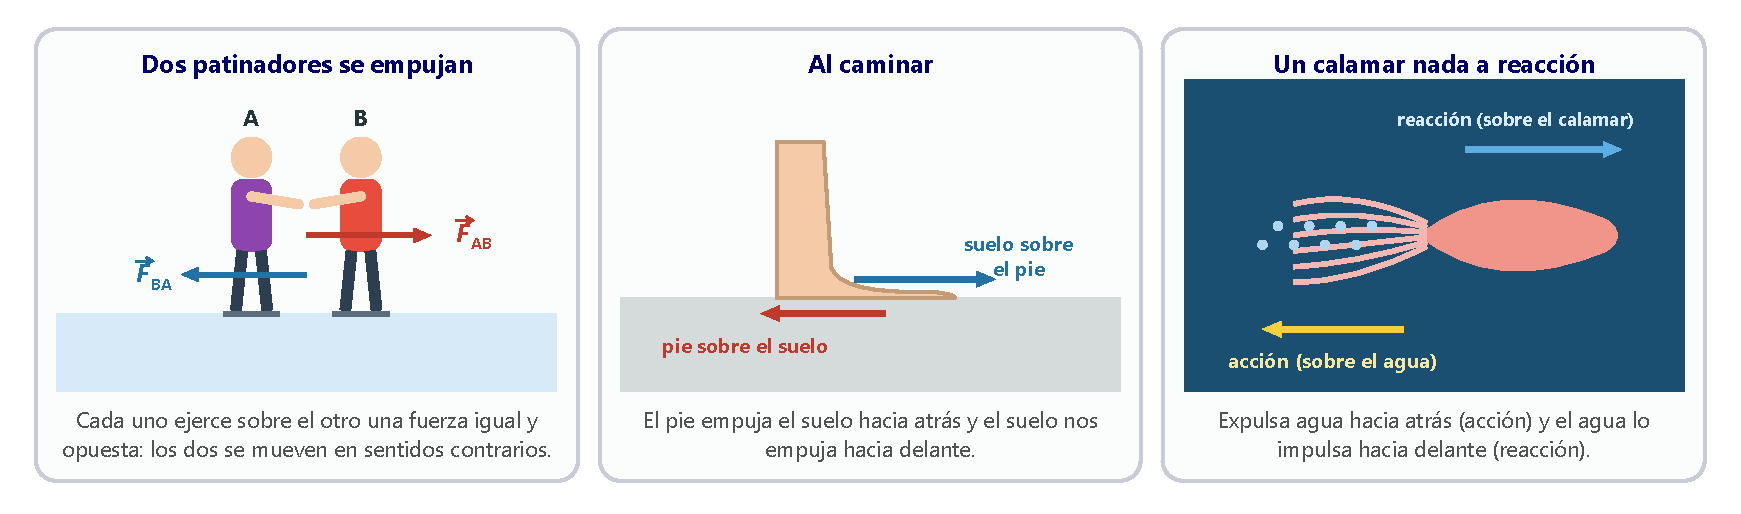
\includegraphics[width=\textwidth]{images/UD8/accion_reaccion}
    \caption{Ejemplos de parejas de fuerzas de acción y reacción.}
    \label{fig:accion_reaccion}
\end{figure}

Al caminar empujamos el suelo hacia atrás y el suelo nos empuja hacia delante; no vemos moverse la Tierra porque su masa es enorme. Al saltar de una barca al embarcadero, empujamos la barca hacia atrás y la barca nos empuja hacia delante.

\begin{example}
    \textbf{Las tres leyes al tirar de una maleta con ruedas.} \emph{Primera ley}: la maleta parada tiende a seguir en reposo, así que hay que tirar con una fuerza mayor que el rozamiento. \emph{Segunda ley}: mientras hay fuerza neta, la maleta acelera. Cuando tiramos justo con la fuerza que compensa el rozamiento, la fuerza neta es nula y la maleta sigue a velocidad constante (primera ley). \emph{Tercera ley}: la maleta tira de nosotros con una fuerza igual y opuesta a la nuestra; no se anulan porque actúan sobre cuerpos distintos.
\end{example}

\begin{exercise}
    Un estudiante razona: «Según la tercera ley de Newton, si tiro de una maleta, la maleta tira de mí con la misma fuerza en sentido opuesto; las dos fuerzas se anulan y nunca podré moverla». ¿Dónde está el error?
    \begin{solu}
        Las fuerzas de acción y reacción \textcolor{red}{actúan sobre cuerpos distintos} (una sobre la maleta y otra sobre el estudiante), así que \textcolor{red}{no se anulan}. Para saber si la maleta se mueve hay que fijarse solo en las fuerzas que actúan \emph{sobre la maleta}: nuestra fuerza y el rozamiento.
    \end{solu}
\end{exercise}

\begin{exercise}
    Un chico y una chica patinan sobre hielo unidos por una cuerda. El chico, de \qty{60}{\kg}, tira de la chica, de \qty{40}{\kg}, con una fuerza de \qty{12}{\newton}.
    \begin{enumerate}[label=\alph*)]
        \item ¿Qué aceleración adquiere la chica?
        \item ¿Qué fuerza actúa sobre el chico? ¿Qué aceleración adquiere él?
    \end{enumerate}
    \begin{solu}
        a) \(a = \frac{12}{40} = \textcolor{red}{\qty{0.3}{\m\per\square\s}}\). b) Por la tercera ley, la chica tira del chico con \textcolor{red}{\qty{12}{\newton}} en sentido contrario: \(a = \frac{12}{60} = \textcolor{red}{\qty{0.2}{\m\per\square\s}}\).
    \end{solu}
\end{exercise}

\begin{exercise}
    Cuando un caballo tira de un carro, los enganches están tirantes mientras el carro acelera, pero dejan de estarlo si se mueve a velocidad constante. Explícalo con las leyes de Newton.
    \begin{solu}
        Mientras acelera, el caballo tiene que ejercer una fuerza mayor que el rozamiento para que haya fuerza neta (segunda ley): los enganches transmiten esa fuerza y están tirantes (y, por la tercera ley, el carro tira del caballo con la misma fuerza). A velocidad constante, la fuerza neta es nula (primera ley): el caballo solo compensa el pequeño rozamiento de las ruedas y los enganches casi no se tensan.
    \end{solu}
\end{exercise}

\begin{exercise}
    Indica si son verdaderas o falsas y justifícalo:
    \begin{enumerate}[label=\alph*)]
        \item las fuerzas de acción y reacción nunca se anulan porque sus direcciones son diferentes;
        \item la aceleración de un cuerpo tiene siempre la dirección y el sentido de la fuerza neta;
        \item si ninguna fuerza actúa sobre un cuerpo, este está en reposo.
    \end{enumerate}
    \begin{solu}
        a) \textcolor{red}{Falsa}: tienen la misma dirección; no se anulan porque actúan sobre cuerpos distintos. b) \textcolor{red}{Verdadera} (segunda ley). c) \textcolor{red}{Falsa}: puede estar en reposo \emph{o moverse con MRU}.
    \end{solu}
\end{exercise}

%========================================================================================
\section{Una fuerza llamada peso}
%========================================================================================

Todos los cuerpos de la superficie terrestre están sometidos a la atracción gravitatoria de la Tierra, que les comunica la aceleración de la gravedad, \(g = \qty{9.8}{\m\per\square\s}\).

\begin{definition}[Peso]
    El \textbf{peso} es la fuerza con la que la Tierra (u otro astro) atrae a un cuerpo. Se mide en newtons y su módulo es:
    \[ P = m \cdot g \]
\end{definition}

\textbf{No hay que confundir masa y peso.} La \textbf{masa} mide la cantidad de materia de un cuerpo, es una magnitud \textbf{escalar}, se mide en kilogramos con una balanza y es la misma en cualquier lugar. El \textbf{peso} es una fuerza, una magnitud \textbf{vectorial}, se mide en newtons con un dinamómetro y depende del valor de \(g\) en cada lugar. Como vector, el peso tiene:
\begin{itemize}
    \item \textbf{módulo}: \(P = m \cdot g\);
    \item \textbf{punto de aplicación}: el \textbf{centro de gravedad} del cuerpo;
    \item \textbf{dirección}: vertical;
    \item \textbf{sentido}: hacia el centro de la Tierra.
\end{itemize}

\subsection{¿Cómo se identifican las fuerzas que actúan sobre un cuerpo?}

\begin{figure}[H]
    \centering
    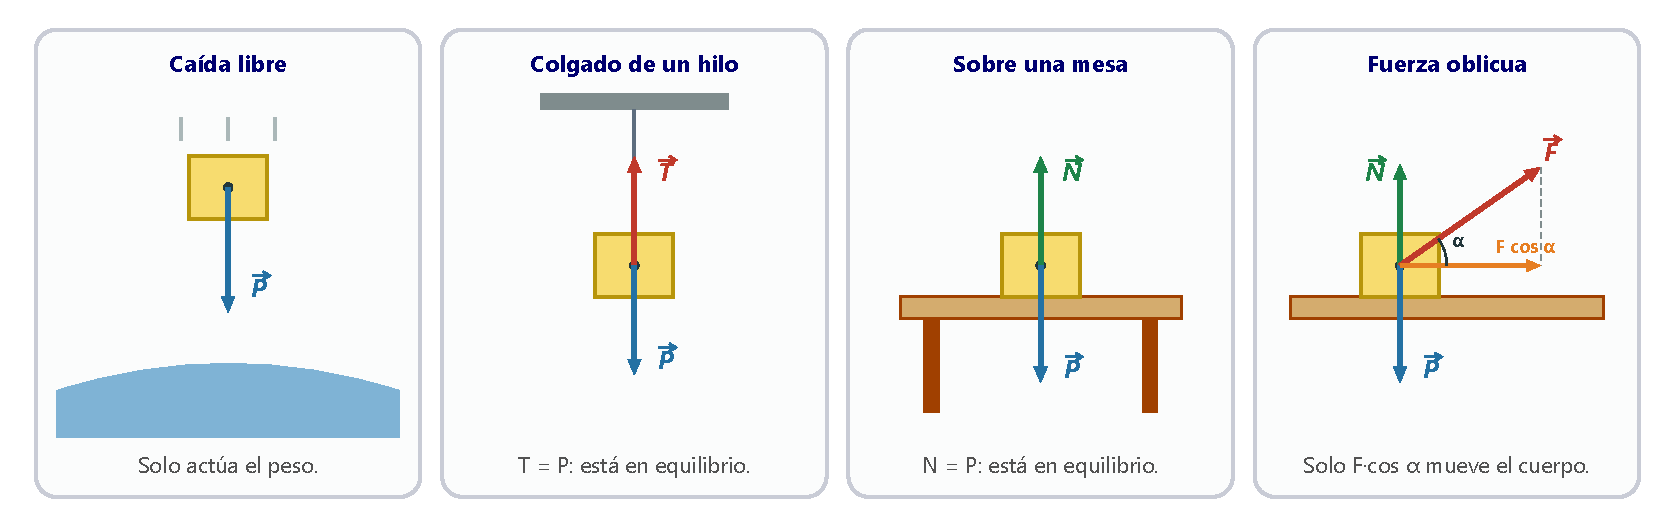
\includegraphics[width=\textwidth]{images/UD8/fuerzas_cuerpos}
    \caption{Fuerzas que actúan sobre un cuerpo en distintas situaciones.}
    \label{fig:fuerzas_cuerpos}
\end{figure}

\begin{itemize}
    \item \textbf{Cuerpo en caída libre.} Solo actúa el peso, \(\vec{P}\), aplicado en el centro de gravedad y dirigido hacia la Tierra. Su reacción, \(\vec{P}'\), es la fuerza con la que el cuerpo atrae a la Tierra, y está aplicada en ella.
    \item \textbf{Cuerpo colgado de un hilo.} Actúan el peso, \(\vec{P}\), y la \textbf{tensión} del hilo, \(\vec{T}\). Como el cuerpo está en reposo, \(T = P\). Sus reacciones son \(\vec{P}'\) (sobre la Tierra) y \(\vec{T}'\) (sobre el hilo).
    \item \textbf{Cuerpo apoyado en una superficie horizontal.} Actúan el peso, \(\vec{P}\), y la fuerza \textbf{normal}, \(\vec{N}\), que ejerce la superficie, perpendicular a ella. Como el cuerpo está en reposo, \(N = P\).
    \item \textbf{Si además empujamos horizontalmente con una fuerza \(F\)}, el peso y la normal se anulan y la fuerza neta es \(F\): \(a = \dfrac{F}{m}\) (sin rozamiento).
    \item \textbf{Si la fuerza forma un ángulo \(\alpha\) con la horizontal}, solo su componente horizontal, \(F \cos\alpha\), hace avanzar el cuerpo: \(a = \dfrac{F\cos\alpha}{m}\) (sin rozamiento).
\end{itemize}

\subsection{Cuerpo apoyado sobre un plano inclinado}

En un plano inclinado un ángulo \(\alpha\), el peso no es perpendicular a la superficie. Conviene descomponerlo en dos componentes (figura~\ref{fig:plano_inclinado}):
\begin{itemize}
    \item \(P_1 = P \sin\alpha = m\,g \sin\alpha\), paralela al plano y hacia abajo;
    \item \(P_2 = P \cos\alpha = m\,g \cos\alpha\), perpendicular al plano.
\end{itemize}
La normal solo equilibra a \(P_2\): \(N = m\,g\cos\alpha\). La componente \(P_1\) no está equilibrada y, si no hay rozamiento, hace bajar el cuerpo con aceleración:
\[ m\,g\sin\alpha = m\,a \;\Rightarrow\; a = g \sin\alpha \]
Esta aceleración solo depende del ángulo de inclinación, \textbf{no de la masa} del cuerpo.

\begin{figure}[H]
    \centering
    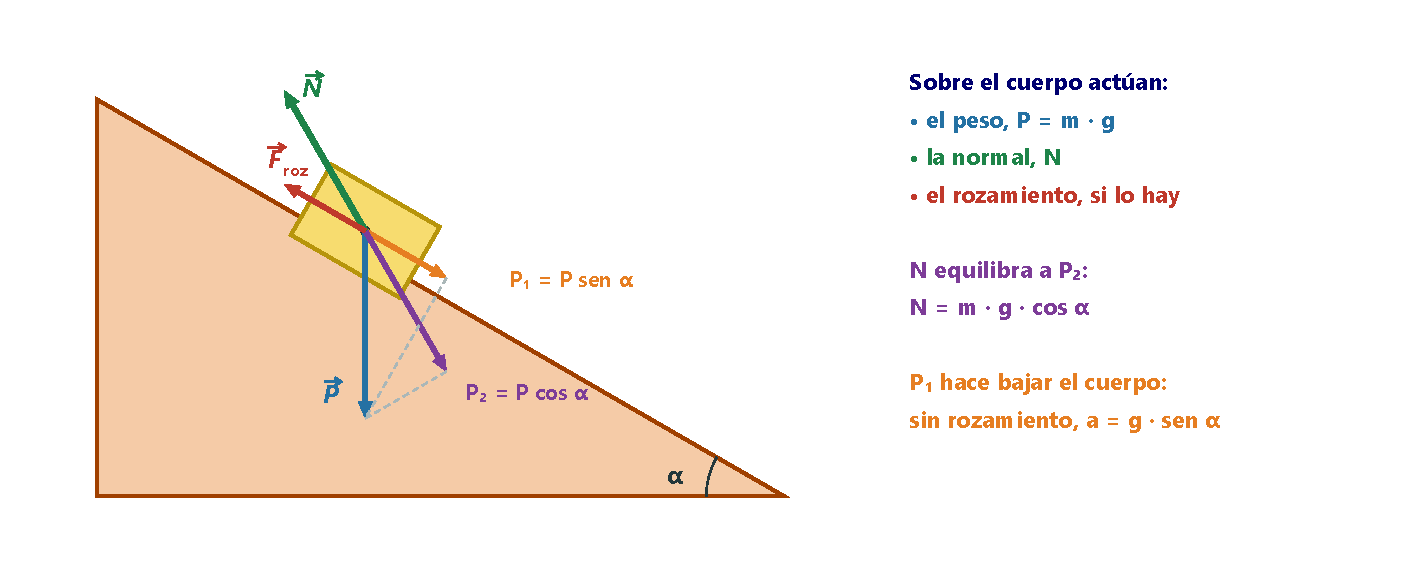
\includegraphics[width=0.9\textwidth]{images/UD8/plano_inclinado}
    \caption{Fuerzas sobre un cuerpo apoyado en un plano inclinado.}
    \label{fig:plano_inclinado}
\end{figure}

\begin{example}
    Calcula la aceleración con la que baja un cuerpo por un plano inclinado \ang{30} sin rozamiento.
    \[ a = g \sin\alpha = \num{9.8} \cdot \sin\ang{30} = \num{9.8} \cdot \num{0.5} = \textcolor{red}{\qty{4.9}{\m\per\square\s}} \]
\end{example}

\begin{exercise}
    ¿Cuánto pesa una persona de \qty{65}{\kg} en la Tierra (\(g = \qty{9.8}{\m\per\square\s}\))? ¿Y en la Luna (\(g = \qty{1.6}{\m\per\square\s}\))? ¿Cambia su masa?
    \begin{solu}
        Tierra: \(P = 65 \cdot \num{9.8} = \textcolor{red}{\qty{637}{\newton}}\). Luna: \(P = 65 \cdot \num{1.6} = \textcolor{red}{\qty{104}{\newton}}\). Su masa \textcolor{red}{no cambia}: es de \qty{65}{\kg} en los dos sitios.
    \end{solu}
\end{exercise}

\begin{exercise}
    Dibuja las fuerzas que actúan sobre un cuerpo de \qty{8}{\kg} colgado de un hilo. Calcula el peso y la tensión del hilo.
    \begin{solu}
        Actúan el peso, hacia abajo, y la tensión, hacia arriba (como en la figura~\ref{fig:fuerzas_cuerpos}). \(P = 8 \cdot \num{9.8} = \textcolor{red}{\qty{78.4}{\newton}}\); como está en equilibrio, \(T = P = \textcolor{red}{\qty{78.4}{\newton}}\).
    \end{solu}
\end{exercise}

\begin{exercise}
    Calcula la aceleración con la que baja un cuerpo por un plano inclinado \ang{45} sin rozamiento.
    \begin{solu}
        \(a = \num{9.8} \cdot \sin\ang{45} = \num{9.8} \cdot \num{0.707} = \textcolor{red}{\qty{6.93}{\m\per\square\s}}\).
    \end{solu}
\end{exercise}

\begin{exercise}
    Copia y completa la tabla para un cuerpo de \qty{50}{\kg}. ¿En qué lugar intentarías batir tu récord de salto de altura? ¿En cuál no lo intentarías nunca?
    \begin{center}
        % --- tabla antigua ---
        % \begin{tblr}{colspec={lcc}, hlines, vlines, row{1}={bg=ocre!85, fg=white, font=\bfseries}}
            % Lugar & Masa (\unit{\kg}) & Peso (\unit{\newton}) \\
            % Espacio lejos de los astros (\(g \approx 0\)) & 50 & \ldots \\
            % Superficie de la Tierra (\(g = \qty{9.8}{\m\per\square\s}\)) & 50 & \ldots \\
            % Superficie de la Luna (\(g = \qty{1.6}{\m\per\square\s}\)) & 50 & \ldots \\
            % Superficie de Júpiter (\(g = \qty{24.8}{\m\per\square\s}\)) & 50 & \ldots \\
        % \end{tblr}
        % --- tabla nueva ---
        \begin{tabular}{@{}lcc@{}}
            \toprule
            \textbf{Lugar} & \textbf{Masa (\unit{\kg})} & \textbf{Peso (\unit{\newton})} \\
            \midrule
            Espacio lejos de los astros (\(g \approx 0\)) & 50 & \ldots \\[3pt]
            Superficie de la Tierra (\(g = \qty{9.8}{\m\per\square\s}\)) & 50 & \ldots \\[3pt]
            Superficie de la Luna (\(g = \qty{1.6}{\m\per\square\s}\)) & 50 & \ldots \\[3pt]
            Superficie de Júpiter (\(g = \qty{24.8}{\m\per\square\s}\)) & 50 & \ldots \\
            \bottomrule
        \end{tabular}
    \end{center}
    \begin{solu}
        Pesos: \textcolor{red}{0}; \textcolor{red}{\qty{490}{\newton}}; \textcolor{red}{\qty{80}{\newton}}; \textcolor{red}{\qty{1240}{\newton}}. Intentaría batir el récord en la \textcolor{red}{Luna} (donde menos pesaría, aunque fuera de los astros no hay «suelo» del que saltar), y nunca en \textcolor{red}{Júpiter}.
    \end{solu}
\end{exercise}

\begin{exercise}
    Un astronauta está en un lugar del espacio donde la gravedad es la mitad que en la superficie terrestre. Indica si son verdaderas o falsas:
    \begin{enumerate}[label=\alph*)]
        \item su peso es el mismo que en la Tierra;
        \item su masa es el doble;
        \item allí pesa la mitad.
    \end{enumerate}
    \begin{solu}
        a) \textcolor{red}{Falsa}. b) \textcolor{red}{Falsa}: la masa no cambia. c) \textcolor{red}{Verdadera}: \(P = m \cdot \frac{g}{2}\).
    \end{solu}
\end{exercise}

\begin{exercise}
    Indica si son verdaderas o falsas y corrige las falsas:
    \begin{enumerate}[label=\alph*)]
        \item el peso es la cantidad de materia de un cuerpo;
        \item la masa se mide con una balanza comparándola con una masa patrón;
        \item el peso está aplicado en el centro de gravedad y dirigido hacia el centro de la Tierra;
        \item el peso de un cuerpo no depende del lugar donde se encuentre.
    \end{enumerate}
    \begin{solu}
        a) \textcolor{red}{Falsa}: eso es la masa; el peso es la fuerza con que la Tierra atrae al cuerpo. b) \textcolor{red}{Verdadera}. c) \textcolor{red}{Verdadera}. d) \textcolor{red}{Falsa}: depende del valor de \(g\) en ese lugar.
    \end{solu}
\end{exercise}

\begin{exercise}
    Dibuja las fuerzas que actúan sobre un cuerpo de \qty{10}{\kg} apoyado en una superficie horizontal sin rozamiento, al que se aplica una fuerza horizontal de \qty{20}{\newton}. ¿Con qué aceleración se mueve?
    \begin{solu}
        Actúan el peso (\qty{98}{\newton}, hacia abajo), la normal (\qty{98}{\newton}, hacia arriba) y la fuerza aplicada. Las dos primeras se anulan: \(a = \frac{20}{10} = \textcolor{red}{\qty{2}{\m\per\square\s}}\).
    \end{solu}
\end{exercise}

\begin{exercise}
    A un cuerpo de \qty{5}{\kg} apoyado en una superficie horizontal sin rozamiento se le aplica una fuerza de \qty{20}{\newton} que forma \ang{30} con la horizontal. ¿Con qué aceleración se mueve?
    \begin{solu}
        Solo la componente horizontal produce el movimiento: \(F\cos\ang{30} = 20 \cdot \num{0.866} = \qty{17.3}{\newton}\); \(a = \frac{\num{17.3}}{5} = \textcolor{red}{\qty{3.46}{\m\per\square\s}}\).
    \end{solu}
\end{exercise}

\begin{exercise}
    Un cuerpo de \qty{20}{\kg} apoyado en un plano inclinado \ang{30} sin rozamiento se empuja hacia arriba con una fuerza de \qty{200}{\newton} paralela al plano. ¿Con qué aceleración sube?
    \begin{solu}
        \(P_1 = 20 \cdot \num{9.8} \cdot \num{0.5} = \qty{98}{\newton}\) hacia abajo. \(F_\text{neta} = 200 - 98 = \qty{102}{\newton}\); \(a = \frac{102}{20} = \textcolor{red}{\qty{5.1}{\m\per\square\s}}\).
    \end{solu}
\end{exercise}

\begin{exercise}
    ¿Qué fuerza paralela al plano hay que aplicar a un cuerpo de \qty{10}{\kg} para que suba por un plano inclinado \ang{30} sin rozamiento con una aceleración de \qty{5.1}{\m\per\square\s}? ¿Y para que suba con velocidad constante?
    \begin{solu}
        \(F - m g \sin\ang{30} = m a \Rightarrow F = 10 \cdot \num{5.1} + 10 \cdot \num{9.8} \cdot \num{0.5} = 51 + 49 = \textcolor{red}{\qty{100}{\newton}}\). Con velocidad constante, \(a = 0\): \(F = m g \sin\alpha = \textcolor{red}{\qty{49}{\newton}}\).
    \end{solu}
\end{exercise}

%========================================================================================
\section{¿Por qué se paran los cuerpos? La fuerza de rozamiento}
%========================================================================================

Según la primera ley, un cuerpo con MRU debería seguir moviéndose indefinidamente; y, según la segunda, cualquier fuerza, por pequeña que sea, debería acelerarlo. Sin embargo, una pelota que rueda acaba parándose, y un mueble pesado no se mueve si lo empujamos suavemente. La causa es la \textbf{fuerza de rozamiento}.

\begin{definition}[Fuerza de rozamiento]
    Es la fuerza que aparece en la superficie de contacto entre dos cuerpos cuando uno se desliza, o tiende a deslizarse, sobre el otro. Es \textbf{paralela} a las superficies en contacto y de \textbf{sentido opuesto} al movimiento.
\end{definition}

\subsection{¿De qué depende la fuerza de rozamiento?}

Con un bloque sobre una mesa unido a un portapesas mediante un hilo y una polea, añadimos pesas hasta que el bloque empieza a deslizar (figura~\ref{fig:rozamiento_montaje}). En ese momento, la fuerza aplicada es igual a la de rozamiento. Así se comprueba que la fuerza de rozamiento:
\begin{itemize}
    \item depende de la \textbf{naturaleza} de las superficies en contacto y de su pulimento;
    \item \textbf{no depende del área} de las superficies en contacto (da igual sobre qué cara apoyemos el bloque);
    \item es \textbf{proporcional a la fuerza normal} con la que una superficie aprieta a la otra:
    \[ F_\text{roz} = \mu \cdot N \]
    donde \(\mu\) es el \textbf{coeficiente de rozamiento}, que no tiene unidades y depende de las superficies en contacto. Sobre una superficie horizontal, \(N = m\,g\) y \(F_\text{roz} = \mu\,m\,g\).
\end{itemize}

\begin{figure}[H]
    \centering
    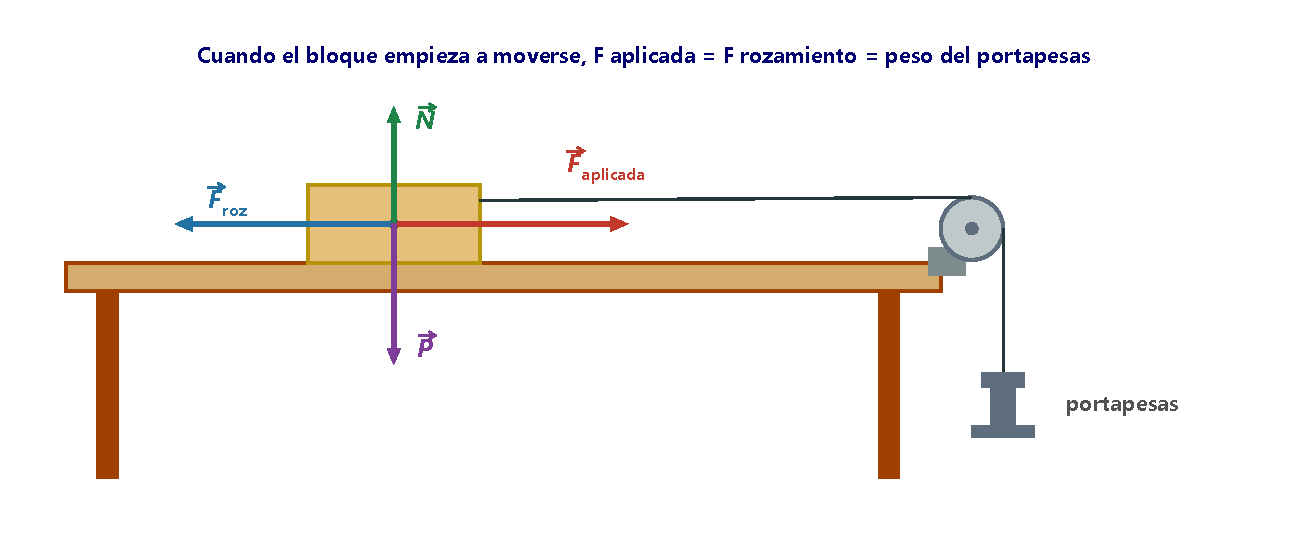
\includegraphics[width=0.85\textwidth]{images/UD8/rozamiento_montaje}
    \caption{Montaje para estudiar la fuerza de rozamiento.}
    \label{fig:rozamiento_montaje}
\end{figure}

\subsection{Problemas con rozamiento en planos horizontales e inclinados}

\begin{marker}
    \textbf{Cómo resolver problemas de dinámica.}
    \begin{enumerate}[label=\arabic*.]
        \item Haz un esquema de la situación.
        \item Dibuja todas las fuerzas que actúan sobre el cuerpo y calcula la fuerza neta en la dirección del movimiento.
        \item Aplica la segunda ley de Newton, \(F_\text{neta} = m \cdot a\), para calcular lo que se pide.
    \end{enumerate}
\end{marker}

\begin{example}
    ¿Qué fuerza horizontal hay que aplicar a un cuerpo de \qty{25}{\kg} para que se deslice con velocidad uniforme sobre una superficie horizontal, si \(\mu = \num{0.1}\)?

    Si la velocidad es constante, \(a = 0\) y la fuerza neta es nula: la fuerza aplicada es igual a la de rozamiento.
    \[ F = F_\text{roz} = \mu\,m\,g = \num{0.1} \cdot 25 \cdot \num{9.8} = \textcolor{red}{\qty{24.5}{\newton}} \]
\end{example}

\begin{example}
    A un cuerpo de \qty{4}{\kg} apoyado en un plano horizontal se le aplica una fuerza horizontal de \qty{40}{\newton}. Si \(\mu = \num{0.1}\), ¿qué aceleración adquiere?
    \[ F_\text{roz} = \num{0.1} \cdot 4 \cdot \num{9.8} = \qty{3.92}{\newton}; \quad F_\text{neta} = 40 - \num{3.92} = \qty{36.08}{\newton}; \quad a = \frac{\num{36.08}}{4} = \textcolor{red}{\qty{9.02}{\m\per\square\s}} \]
\end{example}

\begin{example}
    Un cuerpo baja por un plano inclinado \ang{30} bajo la acción de su peso. Si \(\mu = \num{0.2}\), ¿con qué aceleración lo hace?

    Ahora la fuerza neta es \(P_1 - F_\text{roz}\), con \(F_\text{roz} = \mu\,N = \mu\,m\,g\cos\alpha\):
    \[ m\,a = m\,g\sin\alpha - \mu\,m\,g\cos\alpha \;\Rightarrow\; a = \num{9.8}\,(\num{0.5} - \num{0.2} \cdot \num{0.866}) = \textcolor{red}{\qty{3.20}{\m\per\square\s}} \]
    Sin rozamiento serían \qty{4.9}{\m\per\square\s}.
\end{example}

\begin{exercise}
    Indica si son verdaderas o falsas y corrige las falsas. La fuerza de rozamiento\ldots
    \begin{enumerate}[label=\alph*)]
        \item se opone al movimiento;
        \item no depende del peso del cuerpo apoyado sobre una superficie horizontal;
        \item depende del área de las superficies en contacto;
        \item depende de la naturaleza de las superficies en contacto;
        \item tiene un coeficiente que se mide en newtons;
        \item no es un vector;
        \item es perpendicular a las superficies en contacto.
    \end{enumerate}
    \begin{solu}
        a) \textcolor{red}{Verdadera}. b) \textcolor{red}{Falsa}: sobre una superficie horizontal \(N = P\), así que es proporcional al peso. c) \textcolor{red}{Falsa}: no depende del área. d) \textcolor{red}{Verdadera}. e) \textcolor{red}{Falsa}: el coeficiente no tiene unidades. f) \textcolor{red}{Falsa}: es una fuerza y, por tanto, un vector. g) \textcolor{red}{Falsa}: es paralela a las superficies.
    \end{solu}
\end{exercise}

\begin{exercise}
    Un bloque de \qty{5}{\kg} está sobre una mesa (\(\mu = \num{0.1}\)) y tiramos de él horizontalmente con un dinamómetro. ¿Qué marcará el dinamómetro cuando el bloque empiece a deslizar?
    \begin{solu}
        \(F = \mu\,m\,g = \num{0.1} \cdot 5 \cdot \num{9.8} = \textcolor{red}{\qty{4.9}{\newton}}\).
    \end{solu}
\end{exercise}

\begin{exercise}
    ¿Qué fuerza hay que aplicar a un cuerpo de \qty{12}{\kg} para desplazarlo con velocidad uniforme sobre una superficie horizontal si \(\mu = \num{0.15}\)?
    \begin{solu}
        \(F = F_\text{roz} = \num{0.15} \cdot 12 \cdot \num{9.8} = \textcolor{red}{\qty{17.6}{\newton}}\).
    \end{solu}
\end{exercise}

\begin{exercise}
    ¿Qué fuerza horizontal hay que aplicar a un bloque de cemento de \qty{80}{\kg} para que se deslice con velocidad uniforme sobre una superficie horizontal, si \(\mu = \num{0.2}\)? Dibuja todas las fuerzas que actúan sobre el bloque.
    \begin{solu}
        Actúan el peso, la normal, la fuerza aplicada y el rozamiento (como en la figura~\ref{fig:rozamiento_montaje}). \(F = \num{0.2} \cdot 80 \cdot \num{9.8} = \textcolor{red}{\qty{156.8}{\newton}}\).
    \end{solu}
\end{exercise}

\begin{exercise}
    Calcula la fuerza de rozamiento sobre un bloque de \qty{15}{\kg} que se desliza por una superficie horizontal con \(\mu = \num{0.3}\). ¿Y sobre un bloque que pesa \qty{150}{\newton} si \(\mu = \num{0.2}\)?
    \begin{solu}
        \(F_\text{roz} = \num{0.3} \cdot 15 \cdot \num{9.8} = \textcolor{red}{\qty{44.1}{\newton}}\). \quad \(F_\text{roz} = \num{0.2} \cdot 150 = \textcolor{red}{\qty{30}{\newton}}\).
    \end{solu}
\end{exercise}

\begin{exercise}
    Se aplica una fuerza horizontal de \qty{36}{\newton} a un cuerpo de \qty{6}{\kg} que se desplaza por una superficie horizontal con \(\mu = \num{0.2}\). ¿Qué aceleración adquiere?
    \begin{solu}
        \(F_\text{roz} = \num{0.2} \cdot 6 \cdot \num{9.8} = \qty{11.76}{\newton}\); \(a = \frac{36 - \num{11.76}}{6} = \textcolor{red}{\qty{4.04}{\m\per\square\s}}\).
    \end{solu}
\end{exercise}

\begin{exercise}
    Sobre un cuerpo de \qty{8}{\kg} que se mueve por un plano horizontal se aplica una fuerza horizontal de \qty{60}{\newton}. Si \(\mu = \num{0.15}\), ¿qué aceleración adquiere?
    \begin{solu}
        \(F_\text{roz} = \num{0.15} \cdot 8 \cdot \num{9.8} = \qty{11.76}{\newton}\); \(a = \frac{60 - \num{11.76}}{8} = \textcolor{red}{\qty{6.03}{\m\per\square\s}}\).
    \end{solu}
\end{exercise}

\begin{exercise}
    ¿Qué fuerza horizontal hay que aplicar a un cuerpo de \qty{60}{\kg} para que se desplace con velocidad uniforme si \(\mu = \num{0.5}\)?
    \begin{solu}
        \(F = \num{0.5} \cdot 60 \cdot \num{9.8} = \textcolor{red}{\qty{294}{\newton}}\).
    \end{solu}
\end{exercise}

\begin{exercise}
    Un cuerpo baja por un plano inclinado \ang{45} bajo la acción de su peso. Halla su aceleración si \(\mu = \num{0.1}\). Dibuja las fuerzas que actúan sobre él.
    \begin{solu}
        Actúan el peso (descompuesto en \(P_1\) y \(P_2\)), la normal y el rozamiento hacia arriba del plano, como en la figura~\ref{fig:plano_inclinado}.
        \(a = g(\sin\ang{45} - \mu\cos\ang{45}) = \num{9.8}\,(\num{0.707} - \num{0.0707}) = \textcolor{red}{\qty{6.24}{\m\per\square\s}}\).
    \end{solu}
\end{exercise}

\begin{exercise}
    Un cuerpo baja por un plano inclinado \ang{30} bajo la acción de su peso. Halla su aceleración si \(\mu = \num{0.1}\).
    \begin{solu}
        \(a = \num{9.8}\,(\num{0.5} - \num{0.1} \cdot \num{0.866}) = \textcolor{red}{\qty{4.05}{\m\per\square\s}}\).
    \end{solu}
\end{exercise}

\begin{exercise}
    Un cuerpo de \qty{10}{\kg} baja por un plano inclinado \ang{45} con \(\mu = \num{0.1}\). ¿Qué fuerza paralela al plano hay que ejercer para que baje con velocidad constante?
    \begin{solu}
        Con velocidad constante, la fuerza neta es nula: \(F + F_\text{roz} = P_1\).
        \(P_1 = 98 \cdot \num{0.707} = \qty{69.3}{\newton}\); \(F_\text{roz} = \num{0.1} \cdot 98 \cdot \num{0.707} = \qty{6.93}{\newton}\); \(F = \num{69.3} - \num{6.93} = \textcolor{red}{\qty{62.4}{\newton}}\), dirigida \textcolor{red}{hacia arriba del plano}.
    \end{solu}
\end{exercise}

\begin{exercise}
    Calcula la aceleración con la que sube un cuerpo de \qty{10}{\kg} apoyado en un plano inclinado \ang{30} si se le empuja hacia arriba con una fuerza de \qty{200}{\newton} paralela al plano y \(\mu = \num{0.2}\).
    \begin{solu}
        Ahora el rozamiento actúa hacia abajo, como \(P_1\): \(P_1 = 98 \cdot \num{0.5} = \qty{49}{\newton}\); \(F_\text{roz} = \num{0.2} \cdot 98 \cdot \num{0.866} = \qty{16.97}{\newton}\).
        \(a = \frac{200 - 49 - \num{16.97}}{10} = \textcolor{red}{\qty{13.4}{\m\per\square\s}}\).
    \end{solu}
\end{exercise}


%------------------------------------------------


    \chapterimage{images/portada_cabeceras/cabecera_UD9}
    \chapter{El movimiento circular. La gravedad y otras fuerzas}

    %! Author = crist
%! Date = 25/10/2026

\spacing{1.3}
%----------------------------------------------------------------------------------------
%	UNIDAD 9: EL MOVIMIENTO CIRCULAR. LA GRAVEDAD Y OTRAS FUERZAS (4.º ESO)
%   Figuras: images/UD9/*.pdf (fuente HTML en images/UD9/html, SVG en images/UD9/svg)
%   Gráficas con pgfplots: estilo «grafica», definido al inicio de la UD7.
%   Datos usados en toda la unidad: G = 6,67·10^-11 N·m²/kg², M_T = 5,97·10^24 kg, R_T = 6,37·10^6 m.
%----------------------------------------------------------------------------------------

% Mapa conceptual del tema (fuente en images/mapas_conceptuales/html/temas.js)
\begin{figure}[H]
    \centering
    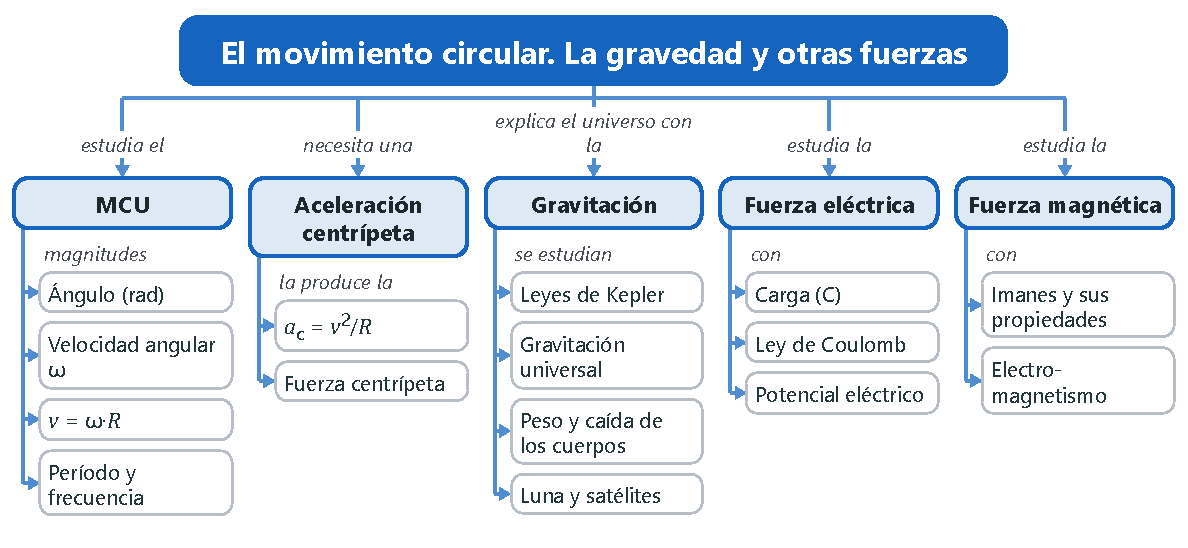
\includegraphics[width=\textwidth]{images/mapas_conceptuales/mapa_UD9}
\end{figure}

%========================================================================================
%\section*{Para empezar: los satélites meteorológicos}
%\addcontentsline{toc}{section}{Para empezar: los satélites meteorológicos}
%========================================================================================
%
%Los \textbf{satélites meteorológicos} envían sin parar datos sobre el estado de la atmósfera en grandes zonas del planeta, y los servicios de predicción del tiempo dependen de esas imágenes.
%
%Los satélites \textbf{Meteosat} de la Agencia Espacial Europea (ESA) son \textbf{geoestacionarios}: giran al mismo ritmo que la Tierra y siempre «miran» la misma zona de la superficie, de la que toman una imagen cada media hora (salvo las regiones polares, que ven mal). Los satélites de \textbf{órbita polar}, en cambio, vuelan mucho más bajos, a unos \qty{800}{\km} de altura, y trabajan por parejas para que sus datos nunca tengan más de seis horas de retraso. Entre todos hacen más de \num{16000} mediciones al día y recorren el planeta entero en 24 horas.
%
%Saber con antelación qué tiempo va a hacer permite tomar medidas: preparar a la población ante un temporal, planificar las cosechas o hacer más segura la navegación. Por eso estos satélites tienen que ver con el \textbf{ODS 11} (\emph{Ciudades y comunidades sostenibles}) y el \textbf{ODS 13} (\emph{Acción por el clima}).
%
%¿Por qué un satélite se mantiene en órbita sin caer? ¿Por qué tarda más en dar una vuelta cuanto más lejos está? En esta unidad lo vamos a entender: estudiaremos el movimiento circular, la fuerza que lo produce y la gravedad, la fuerza que mantiene unidos la Luna, los planetas y los satélites. Terminaremos con otras dos fuerzas de la naturaleza: la eléctrica y la magnética.
%
%\begin{exercise}
%    ¿Para qué sirven los satélites meteorológicos? ¿Son útiles solo para predecir el tiempo de grandes zonas o también a escala local?
%    \begin{solu}
%        Proporcionan \textcolor{red}{datos actualizados continuamente} de las condiciones meteorológicas de grandes zonas. Son imprescindibles tanto para la predicción \textcolor{red}{local como para la de grandes zonas}, porque los modelos de predicción se alimentan de sus imágenes.
%    \end{solu}
%\end{exercise}
%
%\begin{exercise}
%    ¿En qué dos tipos de órbita trabajan los satélites meteorológicos? ¿Qué significa que los Meteosat sean geoestacionarios?
%    \begin{solu}
%        En \textcolor{red}{órbitas geoestacionarias} y en \textcolor{red}{órbitas polares}. Un satélite geoestacionario tarda lo mismo que la Tierra en dar una vuelta (24 horas), por lo que \textcolor{red}{permanece siempre sobre la misma zona} de la superficie.
%    \end{solu}
%\end{exercise}
%
%\begin{exercise}
%    ¿A qué altura vuelan los satélites de órbita polar? ¿Por qué actúan por parejas?
%    \begin{solu}
%        A unos \textcolor{red}{\qty{800}{\km}} de altura. Trabajan por parejas para que los datos que captan \textcolor{red}{no tengan más de seis horas de retraso}.
%    \end{solu}
%\end{exercise}
%
%\begin{exercise}
%    Un satélite no puede evitar un temporal. ¿Por qué, entonces, se relaciona con los ODS 11 y 13? Debatidlo en clase.
%    \begin{solu}
%        Respuesta libre. Anticipar el tiempo permite \textcolor{red}{tomar medidas preventivas} ante temporales, inundaciones u olas de calor, proteger a la población de las ciudades (ODS 11) y adaptarse a los efectos del cambio climático (ODS 13).
%    \end{solu}
%\end{exercise}

%========================================================================================
\section[Características del movimiento circular uniforme]{¿Cuáles son las características del movimiento circular uniforme?}
%========================================================================================

El extremo de la aguja de los minutos de un reloj da una vuelta completa cada hora. Su rapidez es siempre la misma, pero la dirección en la que se mueve cambia en cada instante. Es un ejemplo de movimiento circular uniforme.

\begin{definition}[Movimiento circular uniforme (MCU)]
    Es el movimiento de un cuerpo cuya trayectoria es una \textbf{circunferencia} y que recorre \textbf{arcos iguales en tiempos iguales}.
\end{definition}

El MCU se podría describir con las magnitudes de los movimientos rectilíneos (posición sobre la trayectoria, velocidad\ldots), pero es mucho más sencillo hacerlo con \textbf{magnitudes angulares}.

\begin{figure}[H]
    \centering
    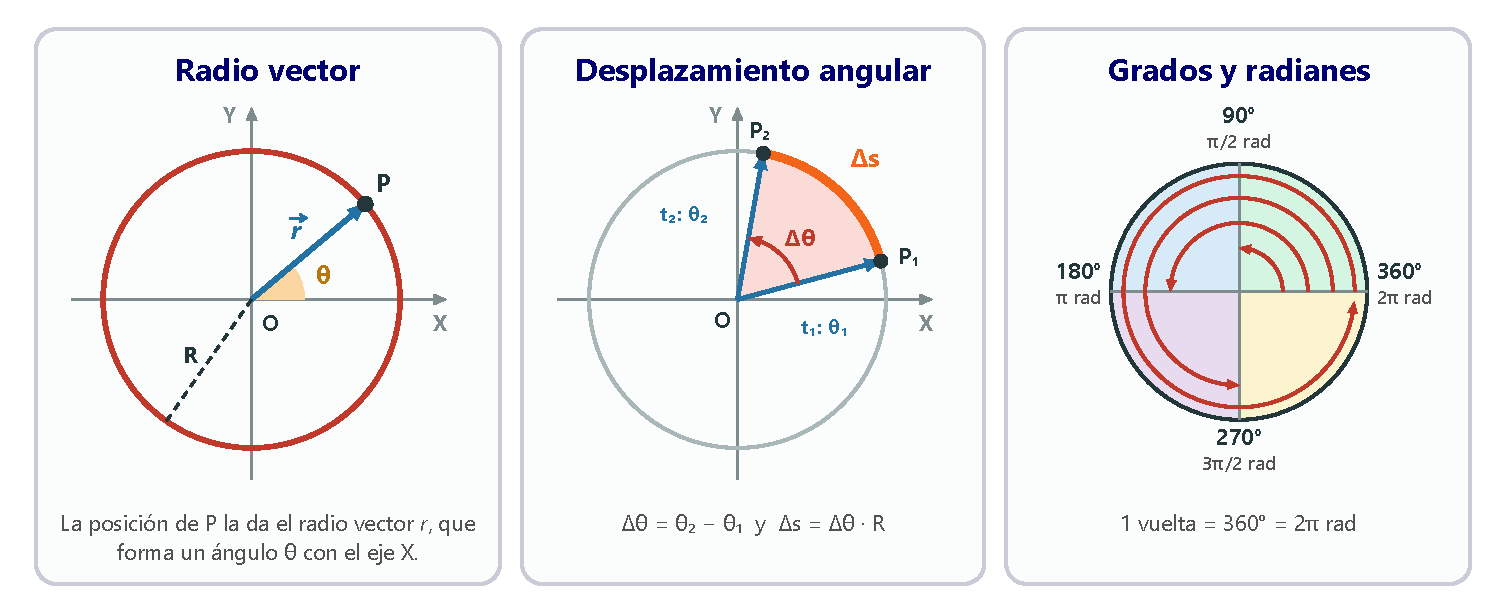
\includegraphics[width=\textwidth]{images/UD9/mcu_magnitudes}
    \caption{Radio vector, desplazamiento angular y medida de ángulos en grados y radianes.}
    \label{fig:mcu_magnitudes}
\end{figure}

\subsection{¿Cómo se indica la posición de un punto? El radio vector}

En un MCU, la posición de un punto P se da con el \textbf{radio vector}, \(\vec{r}\), que tiene su origen en el centro de la circunferencia, O, y su extremo en P (figura~\ref{fig:mcu_magnitudes}). Su módulo es el radio de la circunferencia, \(R\), y forma un ángulo \(\theta\) con el eje X.

\subsection{¿Cómo se mide el cambio de posición? El desplazamiento angular}

Si en el instante \(t_1\) el radio vector forma un ángulo \(\theta_1\) con el eje X y en el instante \(t_2\) forma un ángulo \(\theta_2\), el \textbf{desplazamiento angular} es el ángulo que ha barrido:
\[ \Delta\theta = \theta_2 - \theta_1 \]
Mientras tanto, el punto ha recorrido sobre la circunferencia un arco \(\Delta s\). Las tres magnitudes se relacionan así:
\[ \text{desplazamiento angular} = \frac{\text{arco}}{\text{radio}} \qquad\Rightarrow\qquad \Delta\theta = \frac{\Delta s}{R} \]

\paragraph{¿En qué unidades se mide el desplazamiento angular? El radián.} Un ángulo se puede medir en \textbf{grados} (una circunferencia tiene \ang{360}), en \textbf{revoluciones} o vueltas (una circunferencia es una vuelta) o en \textbf{radianes}, que es la unidad del SI.

\begin{definition}[Radián]
    Un \textbf{radián} (\unit{\radian}) es el ángulo que abarca un arco de longitud igual al radio. Como la longitud de la circunferencia es \(2\pi R\), una vuelta completa son \(2\pi\) radianes:
    \[ 1~\text{vuelta} = \ang{360} = 2\pi~\unit{\radian} \qquad\qquad 1~\unit{\radian} \approx \ang{57.3} \]
\end{definition}

\subsection{¿Qué es la velocidad angular?}

\begin{definition}[Velocidad angular]
    La \textbf{velocidad angular}, \(\omega\), es el ángulo barrido por el radio vector por unidad de tiempo:
    \[ \omega = \frac{\Delta\theta}{\Delta t} \]
    En el MCU es \textbf{constante}. Su ecuación de dimensiones es \([\omega] = \mathrm{T}^{-1}\).
\end{definition}

Además del radián por segundo (\unit{\radian\per\s}), que es la unidad del SI, se usan las \textbf{revoluciones por minuto} (rpm) y las \textbf{revoluciones por segundo} (rps):
\[ 1~\text{rpm} = \frac{1~\text{vuelta}}{1~\text{min}} = \frac{2\pi~\unit{\radian}}{\qty{60}{\s}} = \frac{\pi}{30}~\unit{\radian\per\s} \qquad\qquad 1~\text{rps} = \frac{1~\text{vuelta}}{1~\unit{\s}} = 2\pi~\unit{\radian\per\s} \]

\subsection{Ecuación del MCU}

Como la velocidad angular es constante, el ángulo barrido es proporcional al tiempo:
\[ \Delta\theta = \omega \cdot \Delta t \qquad\Rightarrow\qquad \theta = \theta_0 + \omega \cdot t \]
Si en el instante inicial el ángulo es cero (\(\theta_0 = 0\)), la ecuación queda \(\theta = \omega \cdot t\). Fíjate en que se parece mucho a la ecuación del MRU, \(x = x_0 + v \cdot t\).

\begin{example}
    Un móvil describe un MCU con una velocidad angular de \qty{6}{\radian\per\s}. Calcula el ángulo que barre en \qty{10}{\s} y el tiempo que tarda en dar una vuelta.

    \(\theta = \omega \cdot t = \qty{6}{\radian\per\s} \cdot \qty{10}{\s} = \textcolor{red}{\qty{60}{\radian}}\) (casi diez vueltas). Una vuelta son \(2\pi\) rad, así que:
    \[ t = \frac{\theta}{\omega} = \frac{2\pi~\unit{\radian}}{\qty{6}{\radian\per\s}} = \frac{\pi}{3}~\unit{\s} = \textcolor{red}{\qty{1.05}{\s}} \]
\end{example}

\begin{exercise}
    ¿A cuántos grados equivalen \(\pi\), \(\pi/2\), \(\pi/3\) y \(\pi/4\) radianes? ¿A cuántos radianes equivalen dos vueltas?
    \begin{solu}
        Como \(\pi~\unit{\radian} = \ang{180}\): \(\pi~\unit{\radian} = \textcolor{red}{\ang{180}}\); \(\pi/2 = \textcolor{red}{\ang{90}}\); \(\pi/3 = \textcolor{red}{\ang{60}}\); \(\pi/4 = \textcolor{red}{\ang{45}}\). Dos vueltas son \(2 \cdot 2\pi = \textcolor{red}{4\pi~\unit{\radian}}\).
    \end{solu}
\end{exercise}

\begin{exercise}
    Calcula la velocidad angular de las agujas de las horas, de los minutos y de los segundos de un reloj.
    \begin{solu}
        Cada aguja da una vuelta (\(2\pi\) rad) en 12 h, 1 h y 1 min, respectivamente:
        \[ \omega_h = \frac{2\pi}{\qty{43200}{\s}} = \textcolor{red}{\qty{1.45e-4}{\radian\per\s}} \qquad \omega_{min} = \frac{2\pi}{\qty{3600}{\s}} = \textcolor{red}{\qty{1.75e-3}{\radian\per\s}} \]
        \[ \omega_s = \frac{2\pi}{\qty{60}{\s}} = \textcolor{red}{\qty{0.105}{\radian\per\s}} \]
    \end{solu}
\end{exercise}

\begin{exercise}
    Expresa en radianes por segundo estas velocidades angulares: \num{1.5} rps, 1 rpm, 60 rps y 30 rpm.
    \begin{solu}
        \(\num{1.5}~\text{rps} = \num{1.5} \cdot 2\pi = \textcolor{red}{3\pi~\unit{\radian\per\s}}\); \(1~\text{rpm} = \textcolor{red}{\pi/30~\unit{\radian\per\s}}\); \(60~\text{rps} = \textcolor{red}{120\pi~\unit{\radian\per\s}}\); \(30~\text{rpm} = 30 \cdot \pi/30 = \textcolor{red}{\pi~\unit{\radian\per\s}}\).
    \end{solu}
\end{exercise}

\subsection{¿Qué relación hay entre las magnitudes lineales y las angulares?}

Ya sabemos que \(\Delta s = \Delta\theta \cdot R\). Si dividimos los dos miembros entre el tiempo, obtenemos la relación entre la velocidad lineal y la angular:
\[ v = \omega \cdot R \qquad\qquad \text{velocidad lineal} = \text{velocidad angular} \times \text{radio} \]
En los dos casos, la magnitud lineal es el producto de la angular por el radio.

\begin{center}
    % --- tabla antigua ---
    % \begin{tblr}{colspec={lclcc}, hlines, vlines, row{1}={bg=ocre!85, fg=white, font=\bfseries}}
        % Magnitud lineal & Unidad & Magnitud angular & Unidad & Relación \\
        % Arco recorrido, \(s\) & \unit{\m} & Ángulo barrido, \(\theta\) & \unit{\radian} & \(s = \theta \cdot R\) \\
        % Velocidad lineal, \(v\) & \unit{\m\per\s} & Velocidad angular, \(\omega\) & \unit{\radian\per\s} & \(v = \omega \cdot R\) \\
    % \end{tblr}
    % --- tabla nueva ---
    \begin{tabular}{@{}lclcc@{}}
        \toprule
        \textbf{Magnitud lineal} & \textbf{Unidad} & \textbf{Magnitud angular} & \textbf{Unidad} & \textbf{Relación} \\
        \midrule
        Arco recorrido, \(s\) & \unit{\m} & Ángulo barrido, \(\theta\) & \unit{\radian} & \(s = \theta \cdot R\) \\[3pt]
        Velocidad lineal, \(v\) & \unit{\m\per\s} & Velocidad angular, \(\omega\) & \unit{\radian\per\s} & \(v = \omega \cdot R\) \\
        \bottomrule
    \end{tabular}
\end{center}

\begin{figure}[H]
    \centering
    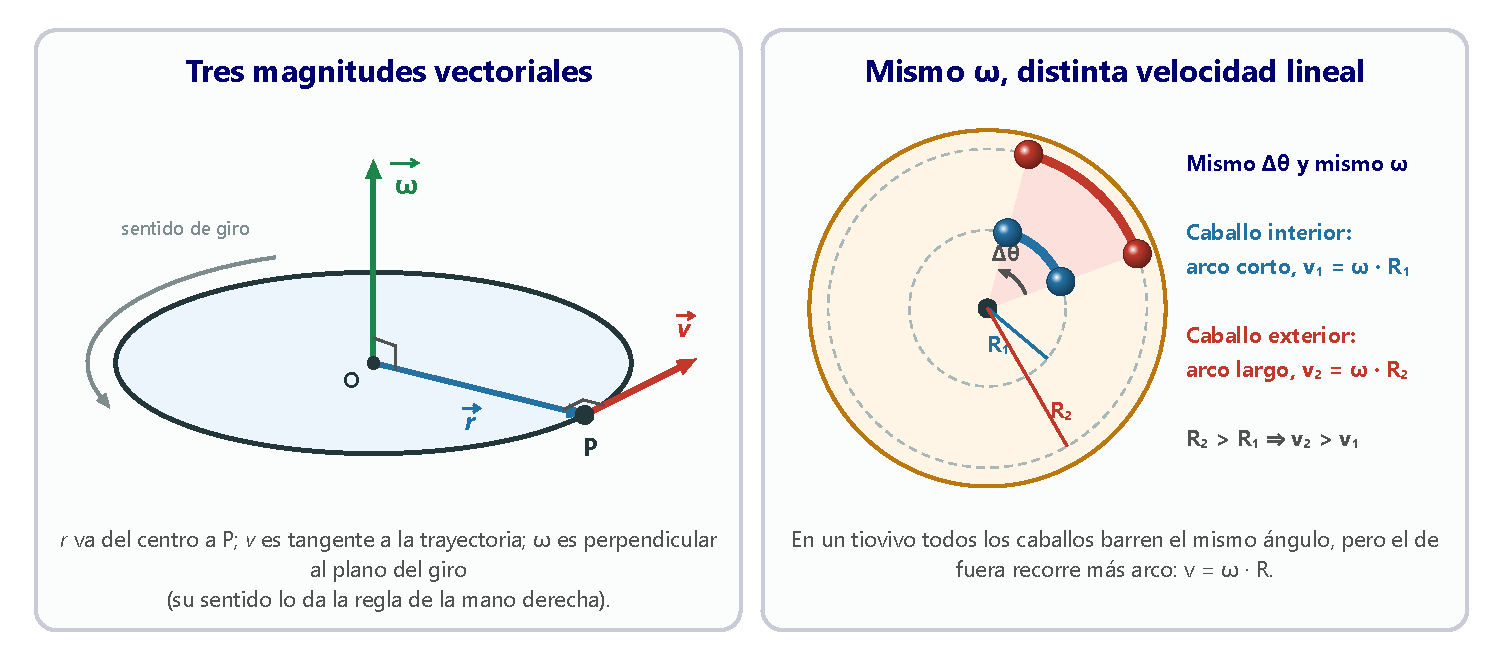
\includegraphics[width=\textwidth]{images/UD9/mcu_vectores}
    \caption{Izquierda: el radio vector, la velocidad lineal y la velocidad angular son vectores. Derecha: en un tiovivo todos los puntos tienen la misma \(\omega\), pero los más alejados del centro tienen más velocidad lineal.}
    \label{fig:mcu_vectores}
\end{figure}

\paragraph{¿Tienen carácter vectorial las magnitudes angulares?} En las fórmulas anteriores usamos solo módulos, pero el radio vector, la velocidad lineal y la velocidad angular son vectores (figura~\ref{fig:mcu_vectores}):
\begin{itemize}
    \item El \textbf{radio vector}, \(\vec{r}\), va del centro de la circunferencia al punto P.
    \item La \textbf{velocidad lineal}, \(\vec{v}\), está aplicada en P, es \textbf{tangente} a la trayectoria y tiene el sentido del movimiento.
    \item La \textbf{velocidad angular}, \(\vec{\omega}\), está aplicada en el centro y es \textbf{perpendicular} al plano de la circunferencia. Su sentido lo da la \textbf{regla de la mano derecha}: si los dedos curvados siguen el giro, el pulgar señala el sentido de \(\vec{\omega}\).
\end{itemize}

\begin{example}
    La Luna da una vuelta alrededor de la Tierra en unos 28 días a una distancia media de \qty{384000}{\km}. Calcula su velocidad angular y su velocidad lineal.
    \[ \omega = \frac{2\pi~\unit{\radian}}{28~\text{días}} \cdot \frac{1~\text{día}}{\qty{86400}{\s}} = \textcolor{red}{\qty{2.6e-6}{\radian\per\s}} \qquad v = \omega \cdot R = \num{2.6e-6} \cdot \qty{3.84e8}{\m} = \textcolor{red}{\qty{997}{\m\per\s}} \]
\end{example}

\begin{example}
    Una plataforma circular de \qty{3}{\m} de radio gira a 15 vueltas por minuto. Calcula la velocidad angular y la velocidad lineal de un punto situado a \qty{1}{\m} del centro y de un punto del borde.
    \[ \omega = \frac{15 \cdot 2\pi~\unit{\radian}}{\qty{60}{\s}} = \frac{\pi}{2}~\unit{\radian\per\s} = \textcolor{red}{\qty{1.57}{\radian\per\s}} \quad \text{(la misma para todos los puntos)} \]
    \[ v_{1\,\mathrm{m}} = \omega \cdot r = \num{1.57} \cdot 1 = \textcolor{red}{\qty{1.6}{\m\per\s}} \qquad v_{3\,\mathrm{m}} = \num{1.57} \cdot 3 = \textcolor{red}{\qty{4.7}{\m\per\s}} \]
\end{example}

\begin{exercise}
    Un satélite artificial da una vuelta a la Tierra cada \qty{5}{\hour} y está a \qty{7570}{\km} del centro de la Tierra. Calcula su velocidad lineal y su velocidad angular.
    \begin{solu}
        \(T = 5 \cdot 3600 = \qty{18000}{\s}\).
        \[ v = \frac{2\pi r}{T} = \frac{2\pi \cdot \qty{7.57e6}{\m}}{\qty{18000}{\s}} = \textcolor{red}{\qty{2642}{\m\per\s}} \qquad \omega = \frac{v}{r} = \frac{2642}{\num{7.57e6}} = \textcolor{red}{\qty{3.5e-4}{\radian\per\s}} \]
    \end{solu}
\end{exercise}

\begin{exercise}
    En una planta embotelladora, una plataforma circular de \qty{25}{\cm} de radio gira a 10 rpm. Calcula la velocidad angular y la velocidad lineal de un punto del borde.
    \begin{solu}
        \[ \omega = \frac{10 \cdot 2\pi~\unit{\radian}}{\qty{60}{\s}} = \frac{\pi}{3}~\unit{\radian\per\s} = \textcolor{red}{\qty{1.05}{\radian\per\s}} \qquad v = \omega \cdot R = \num{1.05} \cdot \qty{0.25}{\m} = \textcolor{red}{\qty{0.26}{\m\per\s}} \]
    \end{solu}
\end{exercise}

\subsection{¿Cuánto tarda en dar una vuelta? Período y frecuencia}

\begin{definition}[Período y frecuencia]
    El \textbf{período}, \(T\), de un MCU es el tiempo que tarda el móvil en dar una vuelta completa. Se mide en segundos.

    La \textbf{frecuencia}, \(f\), es el número de vueltas que da en la unidad de tiempo. Se mide en \textbf{hercios} (\unit{\hertz}): \qty{1}{\hertz} es una vuelta por segundo (\(\unit{\hertz} = \unit{\per\s}\)).

    Son magnitudes inversas:
    \[ T = \frac{1}{f} \qquad\qquad f = \frac{1}{T} \]
\end{definition}

En un período, el móvil recorre la circunferencia completa, \(2\pi R\), y su radio vector barre \(2\pi\) radianes. Por tanto:
\[ v = \frac{2\pi R}{T} = 2\pi R f \qquad\qquad \omega = \frac{2\pi}{T} = 2\pi f \]

\begin{example}
    En un tocadiscos antiguo, un disco de \qty{30}{\cm} de diámetro gira a 33 rpm. Calcula: a) la velocidad angular en \unit{\radian\per\s}; b) la frecuencia y el período; c) la velocidad lineal de un punto del borde.

    a) \(\omega = \dfrac{33 \cdot 2\pi~\unit{\radian}}{\qty{60}{\s}} = \textcolor{red}{\qty{3.46}{\radian\per\s}}\)

    b) \(f = \dfrac{33~\text{vueltas}}{\qty{60}{\s}} = \textcolor{red}{\qty{0.55}{\hertz}}\); \(T = \dfrac{1}{f} = \textcolor{red}{\qty{1.82}{\s}}\)

    c) \(v = \dfrac{2\pi R}{T} = \dfrac{2\pi \cdot \qty{0.15}{\m}}{\qty{1.82}{\s}} = \textcolor{red}{\qty{0.52}{\m\per\s}}\)
\end{example}

\begin{exercise}
    Comprueba que la igualdad \(v = \omega \cdot r\) es homogénea y escribe la ecuación de dimensiones del período y de la frecuencia.
    \begin{solu}
        \([v] = \mathrm{L} \cdot \mathrm{T}^{-1}\); \([\omega] \cdot [r] = \mathrm{T}^{-1} \cdot \mathrm{L}\): los dos miembros tienen las mismas dimensiones, así que \textcolor{red}{es homogénea}. \([T] = \textcolor{red}{\mathrm{T}}\) y \([f] = \textcolor{red}{\mathrm{T}^{-1}}\).
    \end{solu}
\end{exercise}

\begin{exercise}
    Una rueda de \qty{90}{\cm} de diámetro gira a \qty{75}{\radian\per\s}. Calcula el período y la velocidad lineal de un punto de su borde.
    \begin{solu}
        \[ T = \frac{2\pi}{\omega} = \frac{2\pi}{75} = \textcolor{red}{\qty{0.084}{\s}} \qquad v = \omega \cdot R = 75 \cdot \qty{0.45}{\m} = \textcolor{red}{\qty{33.75}{\m\per\s}} \]
    \end{solu}
\end{exercise}

\begin{exercise}
    Una rueda de \qty{1}{\m} de radio gira a 120 vueltas por minuto. Calcula:
    \begin{enumerate}[label=\alph*)]
        \item La frecuencia y el período del movimiento.
        \item La velocidad de un punto del borde de la rueda.
    \end{enumerate}
    \begin{solu}
        a) \(f = \dfrac{120~\text{vueltas}}{\qty{60}{\s}} = \textcolor{red}{\qty{2}{\hertz}}\); \(T = \dfrac{1}{f} = \textcolor{red}{\qty{0.5}{\s}}\).
        b) \(v = \dfrac{2\pi R}{T} = \dfrac{2\pi \cdot 1}{\num{0.5}} = 4\pi = \textcolor{red}{\qty{12.6}{\m\per\s}}\).
    \end{solu}
\end{exercise}

\subsection*{Actividades de consolidación: características del MCU}

\begin{exercise}
    Define qué es el movimiento circular uniforme, el radio vector y el desplazamiento angular.
    \begin{solu}
        El \textcolor{red}{MCU} es el de un cuerpo que describe una circunferencia recorriendo arcos iguales en tiempos iguales. El \textcolor{red}{radio vector} es el vector que va desde el centro de la circunferencia hasta la posición del móvil. El \textcolor{red}{desplazamiento angular} es el ángulo que barre el radio vector entre dos instantes, \(\Delta\theta = \theta_2 - \theta_1\).
    \end{solu}
\end{exercise}

\begin{exercise}
    Una niña montada en un tiovivo barre ángulos de \ang{90}, \ang{180} y \ang{360} a los 5, 10 y 20 segundos de empezar a girar. Calcula:
    \begin{enumerate}[label=\alph*)]
        \item Los radianes que ha barrido en cada caso.
        \item El tiempo que tarda en dar una vuelta.
        \item Su velocidad angular.
    \end{enumerate}
    \begin{solu}
        a) \textcolor{red}{\(\pi/2\) rad}, \textcolor{red}{\(\pi\) rad} y \textcolor{red}{\(2\pi\) rad}. b) \(T = \textcolor{red}{\qty{20}{\s}}\). c) \(\omega = \dfrac{2\pi}{20} = \dfrac{\pi}{10} = \textcolor{red}{\qty{0.31}{\radian\per\s}}\).
    \end{solu}
\end{exercise}

\begin{exercise}
    Un cuerpo con MCU está en el instante \(t_1\) en un punto P\(_1\) cuyo radio vector forma \ang{45} con el eje X, y en el instante \(t_2\), en P\(_2\), a \ang{120}. Calcula el ángulo barrido en grados y en radianes.
    \begin{solu}
        \(\Delta\theta = \ang{120} - \ang{45} = \textcolor{red}{\ang{75}}\). En radianes: \(75 \cdot \dfrac{\pi}{180} = \dfrac{5\pi}{12} = \textcolor{red}{\qty{1.31}{\radian}}\).
    \end{solu}
\end{exercise}

\begin{exercise}
    Una noria gira con MCU a \(\pi/30\) rad/s. Calcula:
    \begin{enumerate}[label=\alph*)]
        \item El ángulo que barre en \qty{6}{\s}.
        \item El tiempo que tardas en dar una vuelta completa montado en una cabina.
    \end{enumerate}
    \begin{solu}
        a) \(\theta = \omega \cdot t = \dfrac{\pi}{30} \cdot 6 = \textcolor{red}{\dfrac{\pi}{5}~\unit{\radian}}\) (\ang{36}). b) \(T = \dfrac{2\pi}{\omega} = \dfrac{2\pi}{\pi/30} = \textcolor{red}{\qty{60}{\s}}\).
    \end{solu}
\end{exercise}

\begin{exercise}
    Un arco de una circunferencia de \qty{20}{\cm} de radio mide \qty{60}{\cm}. Calcula el ángulo correspondiente en radianes y en grados.
    \begin{solu}
        \(\Delta\theta = \dfrac{\Delta s}{R} = \dfrac{60}{20} = \textcolor{red}{\qty{3}{\radian}}\); en grados, \(3 \cdot \dfrac{180}{\pi} = \textcolor{red}{\ang{171.9}}\).
    \end{solu}
\end{exercise}

\begin{exercise}
    Un móvil con MCU da una vuelta completa cada \qty{5}{\s}. Calcula:
    \begin{enumerate}[label=\alph*)]
        \item Su velocidad angular en rad/s, rps y rpm.
        \item El ángulo que barre en \qty{45}{\s}.
    \end{enumerate}
    \begin{solu}
        a) \(\omega = \dfrac{2\pi}{5} = \textcolor{red}{\qty{1.26}{\radian\per\s}} = \textcolor{red}{\num{0.2}~\text{rps}} = \textcolor{red}{12~\text{rpm}}\). b) En \qty{45}{\s} da 9 vueltas: \(\theta = 9 \cdot 2\pi = \textcolor{red}{18\pi~\unit{\radian}}\).
    \end{solu}
\end{exercise}

\begin{exercise}
    Completa la tabla en tu cuaderno:
    \begin{center}
        % --- tabla antigua ---
        % \begin{tblr}{colspec={lccccc}, hlines, vlines, column{1}={bg=ocre!85, fg=white, font=\bfseries}}
            % rpm & 120 & & & & \\
            % rps & & 60 & & 10 & \\
            % rad/s & & & \(\pi\) & & \(\pi/4\) \\
        % \end{tblr}
        % --- tabla nueva ---
        \begin{tabular}{@{}lccccc@{}}
            \toprule
            \textbf{rpm} & 120 &  &  &  &  \\[3pt]
            \textbf{rps} &  & 60 &  & 10 &  \\[3pt]
            \textbf{rad/s} &  &  & \(\pi\) &  & \(\pi/4\) \\
            \bottomrule
        \end{tabular}
    \end{center}
    \begin{solu}
        Se usa que 1 rps = 60 rpm = \(2\pi\) rad/s. Por columnas: 120 rpm = \textcolor{red}{2 rps} = \textcolor{red}{\(4\pi\) rad/s}; 60 rps = \textcolor{red}{3600 rpm} = \textcolor{red}{\(120\pi\) rad/s}; \(\pi\) rad/s = \textcolor{red}{\num{0.5} rps} = \textcolor{red}{30 rpm}; 10 rps = \textcolor{red}{600 rpm} = \textcolor{red}{\(20\pi\) rad/s}; \(\pi/4\) rad/s = \textcolor{red}{1/8 rps} = \textcolor{red}{\num{7.5} rpm}.
    \end{solu}
\end{exercise}

\begin{exercise}
    El extremo del aspa de un ventilador gira con MCU a 60 rpm.
    \begin{enumerate}[label=\alph*)]
        \item Expresa esta velocidad en rad/s.
        \item Calcula el ángulo que barre en \qty{10}{\s}.
        \item Calcula el tiempo que tarda en dar una vuelta.
    \end{enumerate}
    \begin{solu}
        a) \(\omega = \dfrac{60 \cdot 2\pi}{60} = \textcolor{red}{2\pi~\unit{\radian\per\s}}\). b) \(\theta = 2\pi \cdot 10 = \textcolor{red}{20\pi~\unit{\radian}}\). c) \(T = \dfrac{2\pi}{2\pi} = \textcolor{red}{\qty{1}{\s}}\).
    \end{solu}
\end{exercise}

\begin{exercise}
    Un tiovivo gira a 3 rpm. Calcula la velocidad lineal de un niño situado a \qty{75}{\cm}, a \qty{1.5}{\m} y a \qty{2.5}{\m} del centro.
    \begin{solu}
        \(\omega = \dfrac{3 \cdot 2\pi}{60} = \dfrac{\pi}{10}~\unit{\radian\per\s}\), la misma para los tres. Con \(v = \omega \cdot r\):
        \(v_1 = \dfrac{\pi}{10} \cdot \num{0.75} = \textcolor{red}{\qty{0.24}{\m\per\s}}\); \(v_2 = \textcolor{red}{\qty{0.47}{\m\per\s}}\); \(v_3 = \textcolor{red}{\qty{0.79}{\m\per\s}}\).
    \end{solu}
\end{exercise}

\begin{exercise}
    Un satélite de observación de órbita baja (LEO) da una vuelta cada \qty{90}{\minute} a \qty{6570}{\km} del centro de la Tierra. Calcula su velocidad lineal, su velocidad angular y su frecuencia.
    \begin{solu}
        \(T = 90 \cdot 60 = \qty{5400}{\s}\).
        \[ f = \frac{1}{T} = \textcolor{red}{\qty{1.85e-4}{\hertz}} \qquad \omega = \frac{2\pi}{T} = \textcolor{red}{\qty{1.16e-3}{\radian\per\s}} \]
        \[ v = \frac{2\pi r}{T} = \frac{2\pi \cdot \num{6.57e6}}{5400} = \textcolor{red}{\qty{7644}{\m\per\s}} \]
    \end{solu}
\end{exercise}

\begin{exercise}
    Una plataforma circular de \qty{1}{\m} de radio gira a 30 vueltas por minuto. Calcula el período, la velocidad angular y la velocidad lineal de un punto del borde.
    \begin{solu}
        \(f = \dfrac{30}{60} = \qty{0.5}{\hertz} \Rightarrow T = \textcolor{red}{\qty{2}{\s}}\); \(\omega = \dfrac{2\pi}{T} = \textcolor{red}{\qty{3.14}{\radian\per\s}}\); \(v = \omega \cdot R = \textcolor{red}{\qty{3.14}{\m\per\s}}\).
    \end{solu}
\end{exercise}

\begin{exercise}
    La rueda de un coche, de \qty{80}{\cm} de diámetro, gira a 716 rpm. Calcula:
    \begin{enumerate}[label=\alph*)]
        \item La velocidad angular en rad/s.
        \item La velocidad lineal de un punto del borde de la rueda.
        \item El período y la frecuencia.
    \end{enumerate}
    \begin{solu}
        a) \(\omega = \dfrac{716 \cdot 2\pi}{60} = \textcolor{red}{\qty{75}{\radian\per\s}}\). b) \(v = \omega \cdot R = 75 \cdot \num{0.40} = \textcolor{red}{\qty{30}{\m\per\s}}\) (\qty{108}{\km\per\hour}, la velocidad del coche). c) \(f = \dfrac{716}{60} = \textcolor{red}{\qty{11.9}{\hertz}}\); \(T = \dfrac{1}{f} = \textcolor{red}{\qty{0.084}{\s}}\).
    \end{solu}
\end{exercise}

\begin{exercise}
    Una rueda gira a 90 rpm. Calcula la velocidad angular y la velocidad lineal de:
    \begin{enumerate}[label=\alph*)]
        \item Un punto a \qty{10}{\cm} del centro.
        \item Un punto a \qty{20}{\cm} del centro.
        \item El punto central de la rueda.
    \end{enumerate}
    \begin{solu}
        La velocidad angular es la misma en todos los puntos: \(\omega = \dfrac{90 \cdot 2\pi}{60} = 3\pi = \textcolor{red}{\qty{9.42}{\radian\per\s}}\).
        a) \(v = \num{9.42} \cdot \num{0.10} = \textcolor{red}{\qty{0.94}{\m\per\s}}\). b) \(v = \textcolor{red}{\qty{1.88}{\m\per\s}}\). c) \(r = 0 \Rightarrow v = \textcolor{red}{0}\).
    \end{solu}
\end{exercise}

%========================================================================================
\section[La aceleración centrípeta]{¿Puede un movimiento ser uniforme y tener aceleración? La aceleración centrípeta}
%========================================================================================

Sí. El MCU es uniforme porque el módulo de la velocidad no cambia, pero tiene aceleración porque la dirección de la velocidad cambia constantemente.

\subsection{La aceleración centrípeta}

\begin{figure}[H]
    \centering
    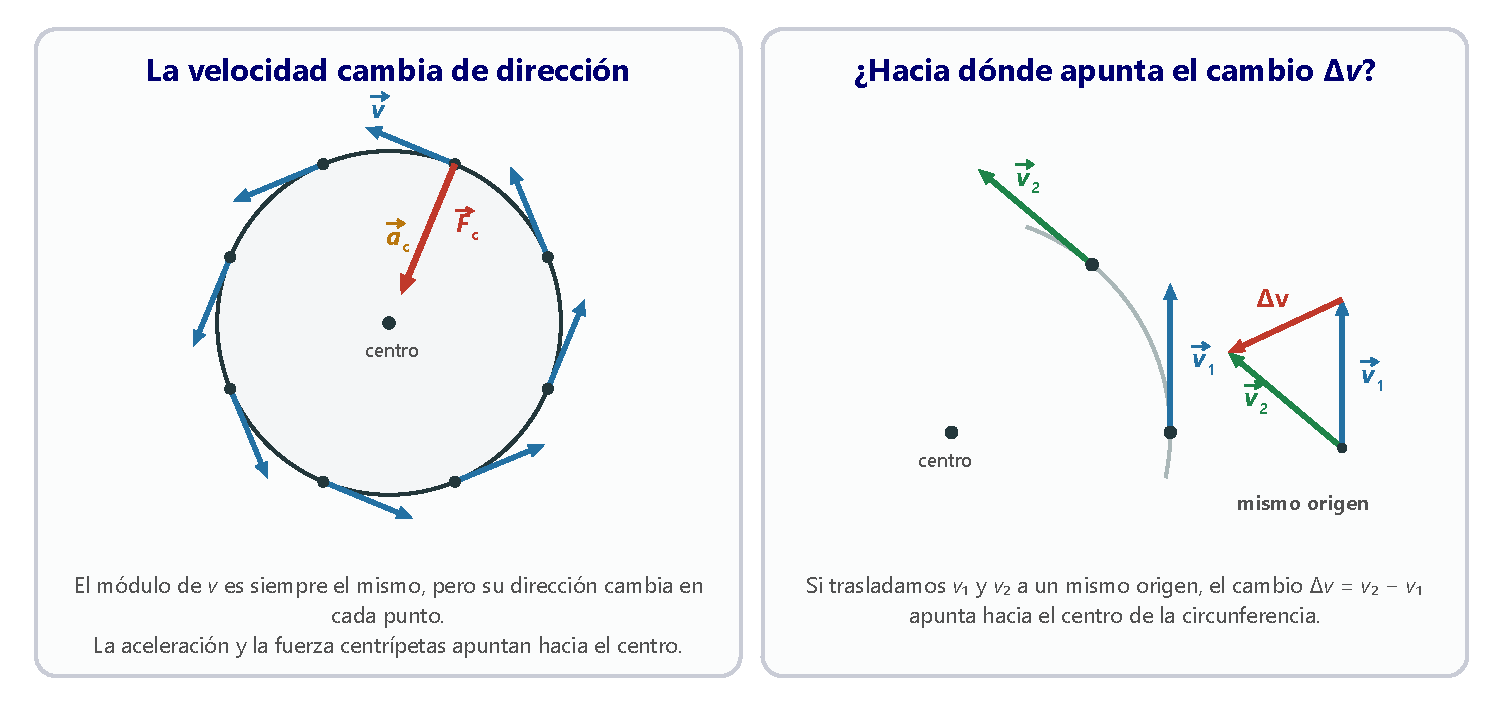
\includegraphics[width=\textwidth]{images/UD9/aceleracion_centripeta}
    \caption{En el MCU la velocidad cambia de dirección en cada punto; ese cambio apunta hacia el centro.}
    \label{fig:aceleracion_centripeta}
\end{figure}

Observa la figura~\ref{fig:aceleracion_centripeta}: el vector velocidad es tangente a la trayectoria en cada punto. Todos los vectores miden lo mismo, pero ninguno apunta en la misma dirección que otro.

\begin{marker}
    En un MCU, el \textbf{módulo} de la velocidad lineal es constante, pero su \textbf{dirección y sentido cambian continuamente}.
\end{marker}

Siempre que cambia la velocidad hay aceleración. Esta se llama \textbf{aceleración centrípeta} o \textbf{normal}, porque es perpendicular a la trayectoria y apunta hacia el \textbf{centro} de la circunferencia. Su módulo es:
\[ a_c = \frac{v^2}{r} \]
donde \(r\) es el radio de la circunferencia. Cuanto más rápido se gira y más cerrada es la curva, mayor es la aceleración centrípeta.

\subsection{¿Qué fuerza produce la aceleración centrípeta? La fuerza centrípeta}

Según la segunda ley de Newton, toda aceleración la produce una fuerza que tiene su misma dirección y sentido. Para que un cuerpo describa un MCU, sobre él tiene que actuar una fuerza dirigida hacia el centro: la \textbf{fuerza centrípeta}, \(\vec{F}_c\).

\begin{definition}[Fuerza centrípeta]
    Es la fuerza resultante, dirigida hacia el centro de la trayectoria, que hace que un cuerpo describa un movimiento circular. Su módulo es:
    \[ F_c = m \cdot a_c = m \cdot \frac{v^2}{r} \]
\end{definition}

La fuerza centrípeta no es una fuerza nueva, sino el papel que cumple alguna fuerza conocida: la tensión de una cuerda, el rozamiento de los neumáticos, la fuerza que hacen las paredes de un tambor o la atracción gravitatoria, como veremos.

\begin{example}
    Un coche de \qty{500}{\kg} toma una curva de \qty{200}{\m} de radio a \qty{72}{\km\per\hour}. Calcula la fuerza centrípeta. ¿Cuáles son su dirección y su sentido?

    Pasamos la velocidad al SI: \(v = 72 \cdot \dfrac{1000}{3600} = \qty{20}{\m\per\s}\).
    \[ F_c = m \cdot \frac{v^2}{r} = \qty{500}{\kg} \cdot \frac{(\qty{20}{\m\per\s})^2}{\qty{200}{\m}} = \textcolor{red}{\qty{1000}{\newton}} \]
    Su dirección es la del radio de la curva y su sentido, \textcolor{red}{hacia el centro} de la curva. En este caso la produce el rozamiento entre los neumáticos y el asfalto.
\end{example}

\begin{exercise}
    Comprueba que las expresiones de la aceleración centrípeta y de la fuerza centrípeta son homogéneas.
    \begin{solu}
        \([a_c] = \dfrac{[v]^2}{[r]} = \dfrac{\mathrm{L}^2\mathrm{T}^{-2}}{\mathrm{L}} = \textcolor{red}{\mathrm{L} \cdot \mathrm{T}^{-2}}\), que son las dimensiones de una aceleración. \([F_c] = \mathrm{M} \cdot \mathrm{L} \cdot \mathrm{T}^{-2}\), las de una fuerza.
    \end{solu}
\end{exercise}

\begin{exercise}
    ¿Existe aceleración centrípeta en un movimiento rectilíneo?
    \begin{solu}
        \textcolor{red}{No}. La aceleración centrípeta aparece cuando cambia la dirección de la velocidad, es decir, cuando la trayectoria es curva.
    \end{solu}
\end{exercise}

\begin{exercise}
    Describe cómo son entre sí las direcciones de la velocidad lineal, la aceleración centrípeta y la fuerza centrípeta en un MCU.
    \begin{solu}
        La velocidad lineal es \textcolor{red}{tangente} a la trayectoria. La aceleración y la fuerza centrípetas tienen la \textcolor{red}{misma dirección}, la del radio, son \textcolor{red}{perpendiculares a la velocidad} y apuntan \textcolor{red}{hacia el centro}.
    \end{solu}
\end{exercise}

\begin{exercise}
    Indica si cada afirmación es verdadera o falsa: «Un MCU es uniforme porque\ldots»
    \begin{enumerate}[label=\alph*)]
        \item \ldots no tiene aceleración.
        \item \ldots el módulo de la velocidad lineal es constante.
        \item \ldots no actúa ninguna fuerza sobre el cuerpo.
        \item \ldots la dirección y el sentido de la velocidad cambian continuamente.
        \item \ldots tiene una aceleración dirigida hacia el centro.
    \end{enumerate}
    \begin{solu}
        a) \textcolor{red}{Falsa}: tiene aceleración centrípeta. b) \textcolor{red}{Verdadera}: por eso es uniforme. c) \textcolor{red}{Falsa}: actúa la fuerza centrípeta. d) \textcolor{red}{Verdadera}, aunque no es la razón de que sea uniforme. e) \textcolor{red}{Verdadera}, aunque tampoco es la razón de que sea uniforme.
    \end{solu}
\end{exercise}

\subsection{¿Qué ocurre cuando deja de actuar la fuerza centrípeta?}

Según la primera ley de Newton, si sobre un cuerpo no actúa ninguna fuerza neta, permanece en reposo o se mueve en línea recta con velocidad constante. Por eso, si la fuerza centrípeta desaparece, el cuerpo \textbf{sale en línea recta, tangente} a la circunferencia, con la velocidad que tenía en ese momento (figura~\ref{fig:sin_fuerza_centripeta}).

\begin{figure}[H]
    \centering
    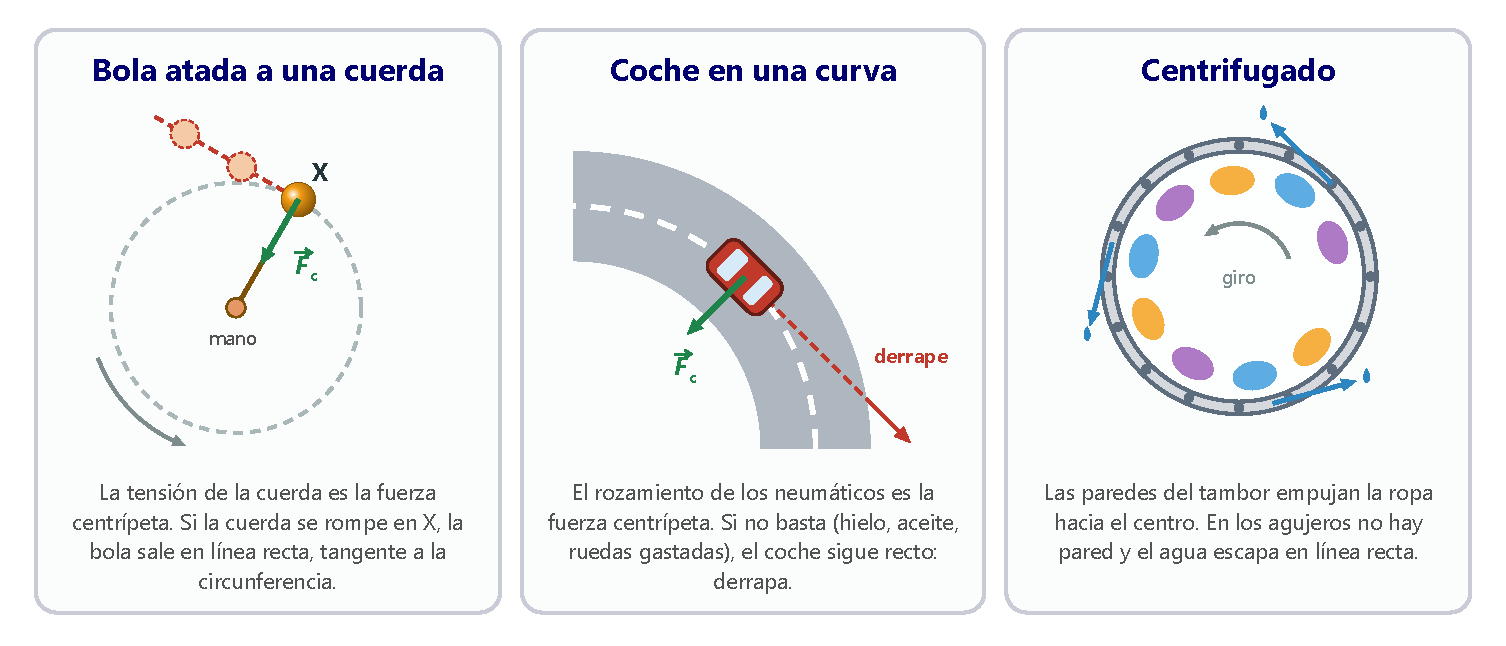
\includegraphics[width=\textwidth]{images/UD9/sin_fuerza_centripeta}
    \caption{Tres situaciones en las que falta la fuerza centrípeta y el cuerpo sigue en línea recta.}
    \label{fig:sin_fuerza_centripeta}
\end{figure}

\begin{exercise}
    Una pelota de \qty{250}{\g} atada a una cuerda de \qty{1}{\m} gira con una velocidad de \qty{1}{\m\per\s}. Calcula el módulo, la dirección y el sentido de la fuerza centrípeta. ¿Qué le pasa a la pelota si se rompe la cuerda?
    \begin{solu}
        \[ F_c = m \cdot \frac{v^2}{r} = \qty{0.25}{\kg} \cdot \frac{(\qty{1}{\m\per\s})^2}{\qty{1}{\m}} = \textcolor{red}{\qty{0.25}{\newton}} \]
        Tiene la dirección de la cuerda y sentido hacia la mano (el centro). Si la cuerda se rompe, la pelota \textcolor{red}{sale en línea recta, tangente} a la circunferencia.
    \end{solu}
\end{exercise}

\begin{exercise}
    Un coche de \qty{650}{\kg} toma una curva de \qty{200}{\m} de radio a \qty{90}{\km\per\hour}. Calcula el módulo de la fuerza centrípeta.
    \begin{solu}
        \(v = \qty{90}{\km\per\hour} = \qty{25}{\m\per\s}\).
        \[ F_c = m \cdot \frac{v^2}{r} = 650 \cdot \frac{25^2}{200} = \textcolor{red}{\qty{2031}{\newton}} \]
    \end{solu}
\end{exercise}

\subsection*{Actividades de consolidación: la aceleración y la fuerza centrípetas}

\begin{exercise}
    En la «esfera de la muerte» del circo, los motoristas dan vueltas por dentro de una gran esfera de rejilla. ¿Qué fuerza les permite girar sin caerse?
    \begin{solu}
        La \textcolor{red}{fuerza centrípeta}, que en este caso la ejerce la pared de la esfera sobre la moto (con la ayuda del peso en la parte alta).
    \end{solu}
\end{exercise}

\begin{exercise}
    Un motorista gira dentro de una esfera de \qty{3}{\m} de radio describiendo un círculo vertical. ¿Cuál es la velocidad mínima que debe llevar en el punto más alto para no caer? Ten en cuenta que caerá si su peso es mayor que la fuerza centrípeta necesaria (\(g = \qty{9.8}{\m\per\square\s}\)).
    \begin{solu}
        En el límite, el peso es justo la fuerza centrípeta:
        \[ m \cdot g = m \cdot \frac{v^2}{r} \quad\Rightarrow\quad v = \sqrt{g \cdot r} = \sqrt{\num{9.8} \cdot 3} = \textcolor{red}{\qty{5.4}{\m\per\s}} \]
    \end{solu}
\end{exercise}

\begin{exercise}
    Investiga en qué deportes y atracciones de feria tiene un papel protagonista la fuerza centrípeta.
    \begin{solu}
        Respuesta libre. Por ejemplo, el \textcolor{red}{lanzamiento de martillo}, el ciclismo en pista (velódromo con curvas peraltadas), el patinaje, las curvas en el automovilismo, las sillas voladoras, la noria o las montañas rusas con bucles.
    \end{solu}
\end{exercise}

\begin{exercise}
    Completa la frase con las palabras \emph{dirección} y \emph{módulo}: «La fuerza centrípeta provoca un cambio en la \ldots{} de la velocidad, pero no en su \ldots».
    \begin{solu}
        «La fuerza centrípeta provoca un cambio en la \textcolor{red}{dirección} de la velocidad, pero no en su \textcolor{red}{módulo}».
    \end{solu}
\end{exercise}

\begin{exercise}
    ¿Verdadero o falso? Justifícalo: «La fuerza que actúa sobre un cuerpo tiene siempre la dirección de su movimiento».
    \begin{solu}
        \textcolor{red}{Falso}. En el movimiento circular, la fuerza centrípeta es perpendicular a la velocidad.
    \end{solu}
\end{exercise}

\begin{exercise}
    Una bola atada a una cuerda gira en un plano horizontal.
    \begin{enumerate}[label=\alph*)]
        \item Completa: «La fuerza que obliga a la bola a describir una circunferencia se llama fuerza \ldots{} Si esta fuerza desaparece, la bola se mueve en línea \ldots, como predice la primera ley de Newton».
        \item ¿Hay que hacer más o menos fuerza si la masa de la bola es mayor? ¿Y si la velocidad es mayor? ¿Y si el radio es menor?
        \item Dibuja la trayectoria de la bola si la cuerda se rompe en un punto X.
    \end{enumerate}
    \begin{solu}
        a) Fuerza \textcolor{red}{centrípeta}; en línea \textcolor{red}{recta}. b) Hay que hacer \textcolor{red}{más fuerza} en los tres casos, porque \(F_c = m v^2 / r\). c) La bola sale en línea recta, \textcolor{red}{tangente} a la circunferencia en X (figura~\ref{fig:sin_fuerza_centripeta}).
    \end{solu}
\end{exercise}

\begin{exercise}
    Calcula la fuerza centrípeta de la actividad anterior si la bola tiene \qty{1}{\kg}, el radio es \qty{1}{\m} y la velocidad, \qty{1}{\m\per\s}.
    \begin{solu}
        \(F_c = m \cdot \dfrac{v^2}{r} = 1 \cdot \dfrac{1^2}{1} = \textcolor{red}{\qty{1}{\newton}}\).
    \end{solu}
\end{exercise}

\begin{exercise}
    Una esfera de \qty{1.5}{\kg} describe una circunferencia de \qty{0.5}{\m} de radio a \qty{2}{\m\per\s}. Calcula la fuerza centrípeta.
    \begin{solu}
        \(F_c = \num{1.5} \cdot \dfrac{2^2}{\num{0.5}} = \textcolor{red}{\qty{12}{\newton}}\).
    \end{solu}
\end{exercise}

\begin{exercise}
    Describe qué le sucede a un cuerpo que se mueve en línea recta si actúa sobre él una fuerza constante:
    \begin{enumerate}[label=\alph*)]
        \item Con la misma dirección y sentido que el movimiento.
        \item Siempre perpendicular al movimiento.
    \end{enumerate}
    \begin{solu}
        a) Sigue en línea recta, pero cada vez más deprisa: \textcolor{red}{MRUA}. b) Cambia de dirección sin cambiar de rapidez: \textcolor{red}{MCU}.
    \end{solu}
\end{exercise}

\begin{exercise}
    Calcula la fuerza centrípeta que actúa sobre una bola de \qty{350}{\g} atada a una cuerda de \qty{1}{\m} que gira a \qty{4}{\m\per\s}.
    \begin{solu}
        \(F_c = \num{0.350} \cdot \dfrac{4^2}{1} = \textcolor{red}{\qty{5.6}{\newton}}\).
    \end{solu}
\end{exercise}

\begin{exercise}
    Un cuerpo de \qty{1.5}{\kg} recorre una circunferencia de \qty{50}{\cm} de radio a 2 rps. Calcula la fuerza centrípeta e indica su dirección y sentido.
    \begin{solu}
        \(\omega = 2 \cdot 2\pi = 4\pi~\unit{\radian\per\s}\); \(v = \omega \cdot r = 4\pi \cdot \num{0.5} = 2\pi~\unit{\m\per\s}\).
        \[ F_c = m \cdot \frac{v^2}{r} = \num{1.5} \cdot \frac{(2\pi)^2}{\num{0.5}} = \textcolor{red}{\qty{118}{\newton}} \]
        Dirección: la del radio; sentido: \textcolor{red}{hacia el centro} de la circunferencia.
    \end{solu}
\end{exercise}

%========================================================================================
\section{El universo mecánico: las leyes de Kepler}
%========================================================================================

En el siglo \textsc{xvi}, \textbf{Nicolás Copérnico} propuso el \textbf{modelo heliocéntrico}: la Tierra no está quieta en el centro del universo, sino que gira, como los demás planetas, alrededor del Sol; el único astro que gira alrededor de la Tierra es la Luna. A comienzos del siglo \textsc{xvii}, \textbf{Johannes Kepler}, a partir de las precisas observaciones de \textbf{Tycho Brahe}, enunció tres leyes que describen cómo se mueven los planetas.

\begin{figure}[H]
    \centering
    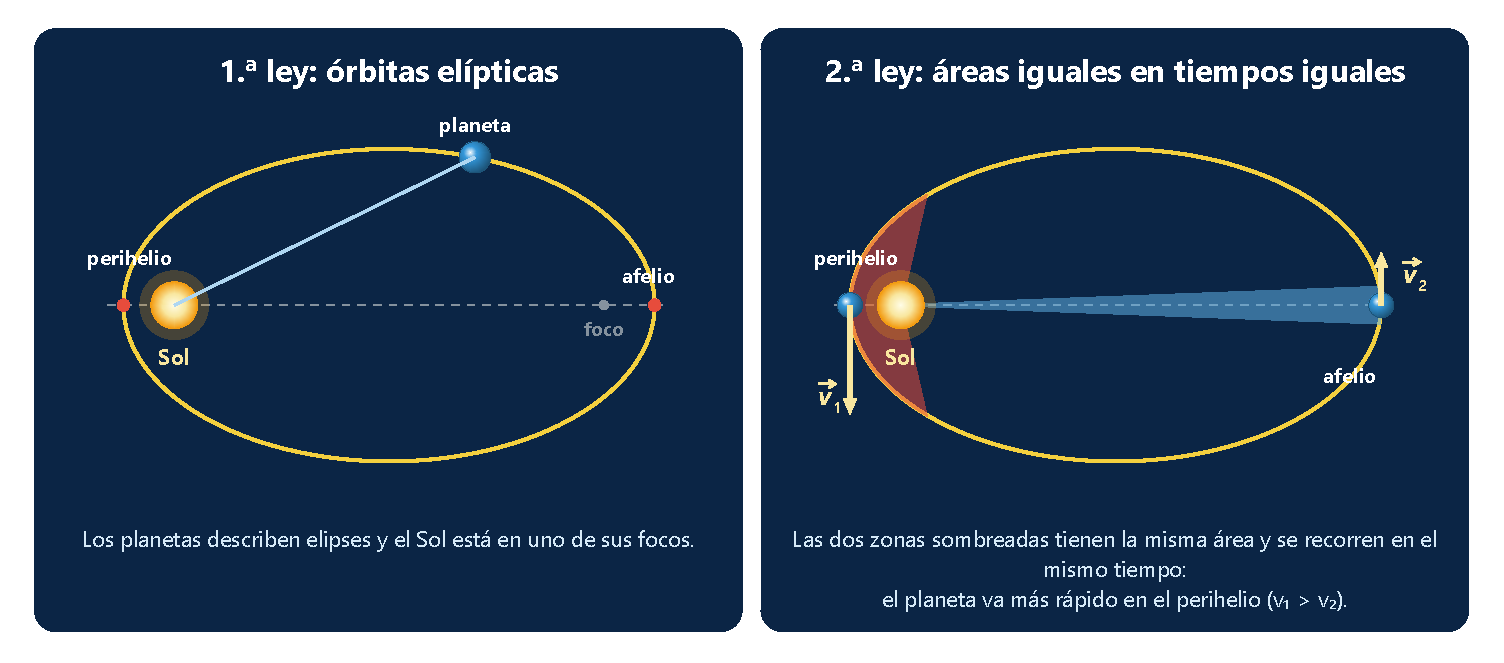
\includegraphics[width=\textwidth]{images/UD9/leyes_kepler}
    \caption{Primera y segunda leyes de Kepler (la elipse está muy exagerada: las órbitas reales son casi circulares).}
    \label{fig:leyes_kepler}
\end{figure}

\begin{definition}[Leyes de Kepler]
    \textbf{Primera ley.} Los planetas giran alrededor del Sol describiendo \textbf{órbitas elípticas}, y el Sol está en uno de los focos de la elipse. El punto de la órbita más cercano al Sol se llama \textbf{perihelio}, y el más alejado, \textbf{afelio}.

    \textbf{Segunda ley.} El radio vector que une el Sol con el planeta barre \textbf{áreas iguales en tiempos iguales}.

    \textbf{Tercera ley.} Para todos los planetas, el cociente entre el cubo del radio medio de la órbita y el cuadrado del período es constante:
    \[ \frac{r^3_{\text{Mercurio}}}{T^2_{\text{Mercurio}}} = \frac{r^3_{\text{Venus}}}{T^2_{\text{Venus}}} = \frac{r^3_{\text{Tierra}}}{T^2_{\text{Tierra}}} = \ldots = \text{constante} \]
\end{definition}

La segunda ley implica que la rapidez del planeta \textbf{no es constante}: es mayor en el perihelio que en el afelio (figura~\ref{fig:leyes_kepler}). La tercera ley dice que cuanto más lejos está un planeta del Sol, más tarda en dar una vuelta.

\begin{remark}
    \textbf{Unidades para medir distancias en el universo.} La \textbf{unidad astronómica} (UA) es la distancia media entre la Tierra y el Sol: \(1~\text{UA} \approx \qty{1.5e11}{\m}\). El \textbf{año luz} es la distancia que recorre la luz en un año: \(\num{9.46e12}~\unit{\km}\).
\end{remark}

\begin{example}
    El cometa Halley tarda unos 76 años en dar una vuelta alrededor del Sol. Calcula su distancia media al Sol, sabiendo que la de la Tierra es \qty{1.5e11}{\m} y su período, 1 año.

    Aplicamos la tercera ley de Kepler a la Tierra y al cometa (podemos dejar los períodos en años):
    \[ \frac{(\qty{1.5e11}{\m})^3}{(1~\text{año})^2} = \frac{r^3_{\text{H}}}{(76~\text{años})^2} \quad\Rightarrow\quad r_{\text{H}} = \sqrt[3]{76^2 \cdot (\num{1.5e11})^3} = \textcolor{red}{\qty{2.69e12}{\m}} \]
\end{example}

\begin{exercise}
    ¿Qué explican las leyes de Kepler: cómo se mueven los planetas o por qué lo hacen?
    \begin{solu}
        Explican \textcolor{red}{cómo se mueven}, no por qué. La causa del movimiento la explicó Newton con la ley de gravitación universal.
    \end{solu}
\end{exercise}

\begin{exercise}
    El radio de la órbita de la Tierra es \qty{1.49e11}{\m} y el de Urano, \qty{2.87e12}{\m}. Expresa estas distancias en UA y calcula el período de Urano en años terrestres.
    \begin{solu}
        La Tierra está a \textcolor{red}{1 UA} y Urano a \(\num{2.87e12}/\num{1.49e11} = \textcolor{red}{\num{19.26}~\text{UA}}\). Con la tercera ley, midiendo en UA y años, la constante vale 1 (la de la Tierra):
        \[ \frac{\num{19.26}^3}{T^2} = \frac{1^3}{1^2} \quad\Rightarrow\quad T = \sqrt{\num{19.26}^3} = \textcolor{red}{\num{84.5}~\text{años}} \]
    \end{solu}
\end{exercise}

\subsection*{Actividades de consolidación: las leyes de Kepler}

\begin{exercise}
    En tiempos de Copérnico ya se conocían las distancias de los planetas al Sol tomando como unidad la distancia Tierra-Sol:
    \begin{center}
        % --- tabla antigua ---
        % \begin{tblr}{colspec={lcccccc}, hlines, vlines, row{1}={bg=ocre!85, fg=white, font=\bfseries}, cell{1}{1}={bg=ocre!85, fg=white}}
            % Planeta & Mercurio & Venus & Tierra & Marte & Júpiter & Saturno \\
            % Distancia al Sol & \num{0.389} & \num{0.724} & 1 & \num{1.525} & \num{5.200} & \num{9.510} \\
        % \end{tblr}
        % --- tabla nueva ---
        \begin{tabular}{@{}lcccccc@{}}
            \toprule
            \textbf{Planeta} & \textbf{Mercurio} & \textbf{Venus} & \textbf{Tierra} & \textbf{Marte} & \textbf{Júpiter} & \textbf{Saturno} \\
            \midrule
            Distancia al Sol & \num{0.389} & \num{0.724} & 1 & \num{1.525} & \num{5.200} & \num{9.510} \\
            \bottomrule
        \end{tabular}
    \end{center}
    Si la distancia Tierra-Sol es \qty{1.5e8}{\km}, calcula la distancia mínima posible entre la Tierra y cada uno de los otros planetas, suponiendo órbitas circulares.
    \begin{solu}
        La distancia mínima se da cuando el planeta y la Tierra están alineados al mismo lado del Sol: es la diferencia de sus distancias al Sol, \(|r - 1| \cdot \num{1.5e8}~\unit{\km}\).
        Mercurio: \(\num{0.611} \cdot \num{1.5e8} = \textcolor{red}{\qty{9.17e7}{\km}}\); Venus: \textcolor{red}{\qty{4.14e7}{\km}}; Marte: \textcolor{red}{\qty{7.88e7}{\km}}; Júpiter: \textcolor{red}{\qty{6.30e8}{\km}}; Saturno: \textcolor{red}{\qty{1.28e9}{\km}}.
    \end{solu}
\end{exercise}

\begin{exercise}
    ¿Verdadero o falso? «El planeta más cercano al Sol es el que tiene el período más corto».
    \begin{solu}
        \textcolor{red}{Verdadero}, según la tercera ley de Kepler: cuanto menor es \(r\), menor es \(T\).
    \end{solu}
\end{exercise}

\begin{exercise}
    Explica con un dibujo la idea de Kepler de que los planetas van más deprisa cuanto más cerca están del Sol. ¿Qué ley la recoge?
    \begin{solu}
        La \textcolor{red}{segunda ley}: el radio vector barre áreas iguales en tiempos iguales. Cerca del Sol (perihelio) el radio vector es corto, así que para barrer la misma área el planeta tiene que recorrer un arco más largo: va \textcolor{red}{más rápido} que en el afelio (figura~\ref{fig:leyes_kepler}).
    \end{solu}
\end{exercise}

\begin{exercise}
    Estos son los radios de las órbitas (en UA) y los períodos que manejaba Kepler. Comprueba con ellos la tercera ley.
    \begin{center}
        % --- tabla antigua ---
        % \begin{tblr}{colspec={lcc}, hlines, vlines, row{1}={bg=ocre!85, fg=white, font=\bfseries}}
            % Planeta & Radio de la órbita (UA) & Período (días) \\
            % Mercurio & \num{0.389} & \num{87.77} \\
            % Venus & \num{0.724} & \num{224.70} \\
            % Tierra & \num{1.000} & \num{365.25} \\
            % Marte & \num{1.525} & \num{686.98} \\
            % Júpiter & \num{5.200} & \num{4332.62} \\
            % Saturno & \num{9.510} & \num{10759.20} \\
        % \end{tblr}
        % --- tabla nueva ---
        \begin{tabular}{@{}lcc@{}}
            \toprule
            \textbf{Planeta} & \textbf{Radio de la órbita (UA)} & \textbf{Período (días)} \\
            \midrule
            Mercurio & \num{0.389} & \num{87.77} \\[3pt]
            Venus & \num{0.724} & \num{224.70} \\[3pt]
            Tierra & \num{1.000} & \num{365.25} \\[3pt]
            Marte & \num{1.525} & \num{686.98} \\[3pt]
            Júpiter & \num{5.200} & \num{4332.62} \\[3pt]
            Saturno & \num{9.510} & \num{10759.20} \\
            \bottomrule
        \end{tabular}
    \end{center}
    \begin{solu}
        Calculamos \(r^3/T^2\) para cada planeta: Mercurio \num{7.64e-6}; Venus \num{7.52e-6}; Tierra \num{7.50e-6}; Marte \num{7.52e-6}; Júpiter \num{7.49e-6}; Saturno \num{7.43e-6} (en UA\(^3\)/día\(^2\)). Son prácticamente iguales, como dice la tercera ley; su valor medio es \textcolor{red}{\(\num{7.5e-6}~\text{UA}^3/\text{día}^2\)}.
    \end{solu}
\end{exercise}

\begin{exercise}
    Imagina que se descubre un planeta diez veces más lejos del Sol que la Tierra. ¿Cuántos años tardaría en dar una vuelta? Usa los datos de la actividad anterior.
    \begin{solu}
        \[ \frac{10^3}{T^2} = \num{7.5e-6} \quad\Rightarrow\quad T = \sqrt{\frac{1000}{\num{7.5e-6}}} = \num{11547}~\text{días} = \textcolor{red}{\num{31.6}~\text{años}} \]
        (También se obtiene directamente: \(T = \sqrt{10^3} = \num{31.6}\) años.)
    \end{solu}
\end{exercise}

\begin{exercise}
    El cometa Swift-Tuttle tiene un período de unos 113 años. Calcula su distancia media al Sol, sabiendo que la de la Tierra es \qty{1.49e11}{\m}.
    \begin{solu}
        \[ \frac{(\num{1.49e11})^3}{1^2} = \frac{r^3}{113^2} \quad\Rightarrow\quad r = \num{1.49e11} \cdot \sqrt[3]{113^2} = \textcolor{red}{\qty{3.48e12}{\m}} \]
    \end{solu}
\end{exercise}

%========================================================================================
\section{La ley de gravitación universal}
%========================================================================================

¿Qué fuerza ejerce el Sol sobre los planetas para que se muevan como dicen las leyes de Kepler? Newton empezó por la Luna. Si sobre ella no actuara ninguna fuerza, se movería en línea recta. Pero describe una órbita casi circular alrededor de la Tierra, así que tiene que haber una fuerza que la atraiga hacia la Tierra. Cuenta la leyenda que, viendo caer una manzana en su jardín, Newton pensó que la fuerza que hace caer la manzana y la que mantiene a la Luna en su órbita son \textbf{la misma}: la Tierra atrae a la Luna igual que atrae a la manzana.

A partir de datos astronómicos y de muchos cálculos, Newton enunció en 1687 la \textbf{ley de gravitación universal}:

\begin{definition}[Ley de gravitación universal]
    Todos los cuerpos del universo se atraen con una fuerza directamente proporcional al producto de sus masas e inversamente proporcional al cuadrado de la distancia que los separa:
    \[ F = G \cdot \frac{m \cdot m'}{r^2} \]
    \(F\) es la fuerza de atracción (\unit{\newton}); \(m\) y \(m'\), las masas de los cuerpos (\unit{\kg}); \(r\), la distancia entre sus centros (\unit{\m}), y \(G\), la \textbf{constante de gravitación universal}:
    \[ G = \qty{6.67e-11}{\newton\square\m\per\square\kg} \]
\end{definition}

\begin{figure}[H]
    \centering
    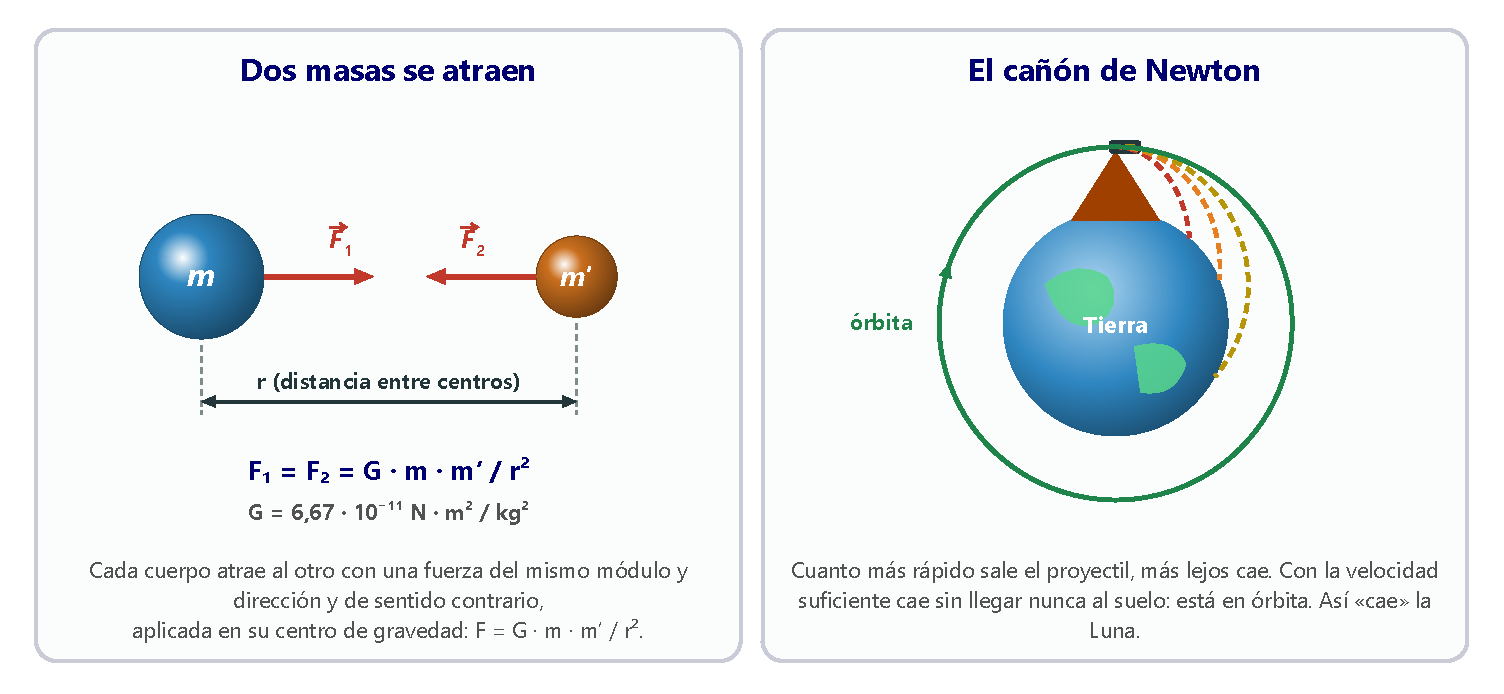
\includegraphics[width=\textwidth]{images/UD9/gravitacion}
    \caption{Izquierda: dos masas se atraen con fuerzas iguales y opuestas. Derecha: el «cañón de Newton»; un proyectil lanzado con la velocidad suficiente queda en órbita.}
    \label{fig:gravitacion}
\end{figure}

\subsection{Características de la fuerza gravitatoria}

\begin{itemize}
    \item Es \textbf{universal}: actúa entre todos los cuerpos que tienen masa.
    \item Es siempre de \textbf{atracción}.
    \item Está aplicada en el \textbf{centro de gravedad} de cada cuerpo y su dirección es la de la \textbf{recta que une sus centros}.
    \item Cumple la tercera ley de Newton: la Tierra atrae al Sol con la misma fuerza con la que el Sol atrae a la Tierra, pero en sentido contrario (figura~\ref{fig:gravitacion}).
    \item Actúa \textbf{a distancia}, sin que los cuerpos estén en contacto, y puede hacer de \textbf{fuerza centrípeta}.
\end{itemize}

\paragraph{¿Es fuerte la fuerza gravitatoria?} \(G\) es muy pequeña, así que la atracción entre dos objetos corrientes es imperceptible: solo se aprecia cuando al menos una de las masas es enorme, como la de un planeta. Las gráficas muestran cómo depende la fuerza de cada variable:
\begin{itemize}
    \item Si la distancia no cambia, la fuerza es \textbf{directamente proporcional} a cada masa: si una masa se duplica, la fuerza se duplica.
    \item Si las masas no cambian, la fuerza es \textbf{inversamente proporcional al cuadrado de la distancia}: si la distancia se duplica, la fuerza se divide entre cuatro. Disminuye muy deprisa al alejarse.
\end{itemize}

\begin{center}
    \begin{tikzpicture}
        \begin{axis}[grafica, width=6.5cm, height=4.6cm, xlabel={masa, \(m\)}, ylabel={fuerza, \(F\)}, xmin=0, xmax=5.2, ymin=0, ymax=5.5, xticklabels={}, yticklabels={}, title={\small \(F\) frente a \(m\) (\(r\) constante)}]
            \addplot[mark=none, domain=0:5, line width=1.4pt, color=red!75!black] {x};
        \end{axis}
    \end{tikzpicture}
    \hspace{0.6cm}
    \begin{tikzpicture}
        \begin{axis}[grafica, width=6.5cm, height=4.6cm, xlabel={distancia, \(r\)}, ylabel={fuerza, \(F\)}, xmin=0, xmax=5.2, ymin=0, ymax=5.5, xticklabels={}, yticklabels={}, title={\small \(F\) frente a \(r\) (masas constantes)}]
            \addplot[mark=none, domain=0.43:5, samples=80, line width=1.4pt, color=red!75!black] {1/x^2};
        \end{axis}
    \end{tikzpicture}
\end{center}

\begin{example}
    Calcula la fuerza de atracción gravitatoria entre el protón y el electrón de un átomo de hidrógeno (\(m_p = \qty{1.67e-27}{\kg}\), \(m_e = \qty{9.1e-31}{\kg}\), distancia \qty{5.3e-11}{\m}).
    \[ F = \num{6.67e-11} \cdot \frac{\num{1.67e-27} \cdot \num{9.1e-31}}{(\num{5.3e-11})^2} = \textcolor{red}{\qty{3.6e-47}{\newton}} \]
\end{example}

\begin{example}
    Calcula la fuerza de atracción entre la Tierra (\qty{5.97e24}{\kg}) y el Sol (\qty{2.0e30}{\kg}), separados \qty{1.5e11}{\m}.
    \[ F = \num{6.67e-11} \cdot \frac{\num{5.97e24} \cdot \num{2.0e30}}{(\num{1.5e11})^2} = \textcolor{red}{\qty{3.5e22}{\newton}} \]
\end{example}

\begin{example}
    ¿Con qué fuerza te atrae la Tierra cuando estás en su superficie (\(R_T = \qty{6.37e6}{\m}\))? Llama \(m\) a tu masa.
    \[ F = \num{6.67e-11} \cdot \frac{\num{5.97e24} \cdot m}{(\num{6.37e6})^2} = \textcolor{red}{\num{9.8} \cdot m}~\unit{\newton} \]
\end{example}

\begin{exercise}
    Compara la intensidad de la atracción gravitatoria entre partículas atómicas y entre cuerpos celestes, usando los dos primeros ejemplos.
    \begin{solu}
        \(\dfrac{\num{3.5e22}}{\num{3.6e-47}} \approx \num{1e69}\): la atracción entre la Tierra y el Sol es unas \textcolor{red}{\(10^{69}\) veces mayor}. Entre partículas, la fuerza gravitatoria es despreciable porque sus masas son minúsculas.
    \end{solu}
\end{exercise}

\begin{exercise}
    Sustituye tu masa en el tercer ejemplo. ¿Qué significado tiene el número \num{9.8} que aparece en el resultado?
    \begin{solu}
        Respuesta libre (por ejemplo, con \qty{60}{\kg}, \(F = \qty{588}{\newton}\)). Esa fuerza es tu \textcolor{red}{peso}, y \num{9.8} es la \textcolor{red}{aceleración de la gravedad}, \(g\), en \unit{\m\per\square\s}.
    \end{solu}
\end{exercise}

\begin{exercise}
    Corrige los enunciados que sean falsos:
    \begin{enumerate}[label=\alph*)]
        \item La constante de gravitación universal depende de dónde estén los cuerpos en el universo.
        \item La Tierra atrae a la Luna con mucha más fuerza que la Luna a la Tierra.
        \item La fuerza gravitatoria puede actuar como fuerza centrípeta sin que los cuerpos estén en contacto.
    \end{enumerate}
    \begin{solu}
        a) Falso: \(G\) \textcolor{red}{es la misma en todo el universo}. b) Falso: las dos fuerzas tienen \textcolor{red}{el mismo módulo} (tercera ley de Newton); lo que ocurre es que a la Luna, con menos masa, esa fuerza le produce más aceleración. c) \textcolor{red}{Verdadero}.
    \end{solu}
\end{exercise}

\begin{exercise}
    En 1797, unos cien años después de que Newton publicara su ley, Henry Cavendish midió el valor de \(G\) con una balanza de torsión. Busca información sobre cómo funciona esa balanza y cómo hizo Cavendish la medida.
    \begin{solu}
        Respuesta libre. Una varilla con dos esferas pequeñas cuelga de un hilo fino; al acercar dos esferas grandes, la atracción gravitatoria hace girar la varilla y retuerce el hilo. Midiendo el ángulo de giro, Cavendish calculó la fuerza y, con ella, \(G\). A esta experiencia se la llamó «pesar la Tierra», porque, conocido \(G\), se puede calcular la masa de la Tierra.
    \end{solu}
\end{exercise}

\begin{exercise}
    El modelo heliocéntrico y la ley de gravitación universal tuvieron varios protagonistas. Investiga las aportaciones de Copérnico, Galileo, Kepler y Newton y el contexto histórico en el que trabajaron.
    \begin{solu}
        Respuesta libre. Copérnico propuso el modelo heliocéntrico (1543); Galileo lo defendió con sus observaciones con el telescopio (satélites de Júpiter, fases de Venus) y fue juzgado por la Inquisición; Kepler descubrió las leyes del movimiento planetario; Newton las explicó con la ley de gravitación universal (1687).
    \end{solu}
\end{exercise}

\subsection*{Actividades de consolidación: la ley de gravitación universal}

\begin{exercise}
    Justifica por qué la atracción gravitatoria disminuye rápidamente al aumentar la distancia entre dos cuerpos.
    \begin{solu}
        Porque es \textcolor{red}{inversamente proporcional al cuadrado de la distancia}: al duplicar la distancia, la fuerza se hace cuatro veces menor; al triplicarla, nueve veces menor.
    \end{solu}
\end{exercise}

\begin{exercise}
    Calcula la fuerza de atracción entre dos cuerpos de \qty{50}{\kg} y \qty{60}{\kg} separados \qty{50}{\cm}.
    \begin{solu}
        \[ F = \num{6.67e-11} \cdot \frac{50 \cdot 60}{\num{0.5}^2} = \textcolor{red}{\qty{8.0e-7}{\newton}} \]
    \end{solu}
\end{exercise}

\begin{exercise}
    Calcula la fuerza con la que se atraen la Tierra y la Luna. Datos: \(M_T = \qty{5.97e24}{\kg}\); \(m_L = \qty{7.20e22}{\kg}\); \(d = \qty{3.84e8}{\m}\).
    \begin{solu}
        \[ F = \num{6.67e-11} \cdot \frac{\num{5.97e24} \cdot \num{7.20e22}}{(\num{3.84e8})^2} = \textcolor{red}{\qty{1.94e20}{\newton}} \]
    \end{solu}
\end{exercise}

\begin{exercise}
    Compara los resultados de las dos actividades anteriores. ¿Qué conclusión sacas?
    \begin{solu}
        La fuerza entre la Tierra y la Luna es unas \(10^{26}\) veces mayor. La gravedad solo es apreciable cuando intervienen \textcolor{red}{masas muy grandes}, como las de los astros.
    \end{solu}
\end{exercise}

\begin{exercise}
    Una masa de \qty{200}{\kg} está a \qty{10}{\m} de otra de \qty{150}{\kg}. ¿Con qué fuerza se atraen? ¿Dónde está aplicada cada fuerza? ¿Cuáles son su dirección y su sentido?
    \begin{solu}
        \[ F = \num{6.67e-11} \cdot \frac{200 \cdot 150}{10^2} = \textcolor{red}{\qty{2.0e-8}{\newton}} \]
        Hay dos fuerzas iguales, una \textcolor{red}{aplicada en el centro de gravedad de cada cuerpo}. Su dirección es la de la recta que une los centros y su sentido, \textcolor{red}{hacia el otro cuerpo}.
    \end{solu}
\end{exercise}

\begin{exercise}
    La Luna (\qty{7.3e22}{\kg}) está a \qty{3.9e8}{\m} del centro de la Tierra (\qty{5.97e24}{\kg}). ¿A qué distancia del centro de la Tierra se anulan las atracciones de los dos astros sobre un cuerpo?
    \begin{solu}
        Llamamos \(x\) a la distancia desde la Tierra; desde la Luna será \(d - x\). Igualamos las dos atracciones (la masa del cuerpo y \(G\) se simplifican):
        \[ \frac{M_T}{x^2} = \frac{m_L}{(d - x)^2} \quad\Rightarrow\quad \frac{x}{d - x} = \sqrt{\frac{M_T}{m_L}} = \sqrt{\frac{\num{5.97e24}}{\num{7.3e22}}} = \num{9.04} \]
        \[ x = \num{9.04} \cdot (d - x) \quad\Rightarrow\quad x = \frac{\num{9.04} \cdot \num{3.9e8}}{\num{10.04}} = \textcolor{red}{\qty{3.51e8}{\m}} \]
        Es decir, a unos \qty{351000}{\km} de la Tierra, mucho más cerca de la Luna, que tiene menos masa.
    \end{solu}
\end{exercise}

%========================================================================================
\section{La síntesis newtoniana}
%========================================================================================

Con sus tres leyes de la dinámica y la ley de gravitación universal, Newton explicó con las mismas ideas fenómenos que hasta entonces parecían no tener nada que ver: la caída de los cuerpos en la Tierra, el movimiento de la Luna, el de los planetas y el de los cometas. A esta unificación se la llama \textbf{síntesis newtoniana}.

\subsection{La caída y el peso de los cuerpos}

Los objetos caen porque la Tierra los atrae: el \textbf{peso} es la fuerza gravitatoria con la que la Tierra atrae a un cuerpo. En la unidad anterior vimos que \(P = m \cdot g\). Si lo igualamos a la ley de gravitación, siendo \(M\) la masa del planeta y \(R\) su radio:
\[ m \cdot g = G \cdot \frac{M \cdot m}{R^2} \quad\Rightarrow\quad g = G \cdot \frac{M}{R^2} \]
Para la Tierra:
\[ g_0 = \num{6.67e-11} \cdot \frac{\num{5.97e24}}{(\num{6.37e6})^2} = \qty{9.8}{\m\per\square\s} \]

\begin{marker}
    \textbf{La gravedad a una altura \(h\) y en otros astros.} A una altura \(h\) sobre la superficie, la distancia al centro es \(R + h\):
    \[ g_h = G \cdot \frac{M}{(R + h)^2} \]
    La misma fórmula sirve para cualquier planeta o satélite con su masa y su radio. \(g\) \textbf{no depende de la masa del cuerpo que cae} y disminuye al alejarnos del astro.
\end{marker}

\begin{center}
    % --- tabla antigua ---
    % \begin{tblr}{colspec={lccc}, hlines, vlines, row{1}={bg=ocre!85, fg=white, font=\bfseries}, column{2-4}={c}}
        % Astro & Masa (\unit{\kg}) & Radio medio (\unit{\m}) & \(g\) en la superficie (\unit{\m\per\square\s}) \\
        % Sol & \num{1.99e30} & \num{6.96e8} & \num{274} \\
        % Mercurio & \num{3.30e23} & \num{2.44e6} & \num{3.7} \\
        % Venus & \num{4.87e24} & \num{6.05e6} & \num{8.9} \\
        % Tierra & \num{5.97e24} & \num{6.37e6} & \num{9.8} \\
        % Luna & \num{7.35e22} & \num{1.74e6} & \num{1.6} \\
        % Marte & \num{6.42e23} & \num{3.39e6} & \num{3.7} \\
        % Júpiter & \num{1.90e27} & \num{6.99e7} & \num{25.9} \\
        % Saturno & \num{5.68e26} & \num{5.82e7} & \num{11.2} \\
        % Urano & \num{8.68e25} & \num{2.54e7} & \num{9.0} \\
        % Neptuno & \num{1.02e26} & \num{2.46e7} & \num{11.2} \\
    % \end{tblr}
    % --- tabla nueva ---
    \begin{tabular}{@{}lccc@{}}
        \toprule
        \textbf{Astro} & \textbf{Masa (\unit{\kg})} & \textbf{Radio medio (\unit{\m})} & \textbf{\(g\) en la superficie (\unit{\m\per\square\s})} \\
        \midrule
        Sol & \num{1.99e30} & \num{6.96e8} & \num{274} \\[3pt]
        Mercurio & \num{3.30e23} & \num{2.44e6} & \num{3.7} \\[3pt]
        Venus & \num{4.87e24} & \num{6.05e6} & \num{8.9} \\[3pt]
        Tierra & \num{5.97e24} & \num{6.37e6} & \num{9.8} \\[3pt]
        Luna & \num{7.35e22} & \num{1.74e6} & \num{1.6} \\[3pt]
        Marte & \num{6.42e23} & \num{3.39e6} & \num{3.7} \\[3pt]
        Júpiter & \num{1.90e27} & \num{6.99e7} & \num{25.9} \\[3pt]
        Saturno & \num{5.68e26} & \num{5.82e7} & \num{11.2} \\[3pt]
        Urano & \num{8.68e25} & \num{2.54e7} & \num{9.0} \\[3pt]
        Neptuno & \num{1.02e26} & \num{2.46e7} & \num{11.2} \\
        \bottomrule
    \end{tabular}
\end{center}

\begin{exercise}
    Busca información sobre cómo explica la ley de gravitación universal el movimiento de los cometas y las mareas.
    \begin{solu}
        Respuesta libre. Los cometas describen \textcolor{red}{órbitas elípticas muy alargadas} alrededor del Sol, como predicen las leyes de Kepler y la gravitación; sus períodos van de unos pocos años a miles de años. Las \textcolor{red}{mareas} se deben a que la Luna (y, en menor medida, el Sol) atrae con más fuerza el agua del lado de la Tierra más cercano que el del lado opuesto: se forman dos abultamientos de agua (mareas altas) y, a \ang{90} de ellos, mareas bajas. Cuando el Sol y la Luna están alineados, las mareas son más intensas (\emph{mareas vivas}).
    \end{solu}
\end{exercise}

\begin{exercise}
    Con los datos de la tabla, calcula la aceleración de la gravedad en la superficie de la Luna, de Marte y de Júpiter, y el peso que tendría en cada uno una persona de \qty{60}{\kg}.
    \begin{solu}
        \[ g_{\text{Luna}} = \num{6.67e-11} \cdot \frac{\num{7.35e22}}{(\num{1.74e6})^2} = \textcolor{red}{\qty{1.62}{\m\per\square\s}} \quad\Rightarrow\quad P = 60 \cdot \num{1.62} = \textcolor{red}{\qty{97}{\newton}} \]
        \[ g_{\text{Marte}} = \num{6.67e-11} \cdot \frac{\num{6.42e23}}{(\num{3.39e6})^2} = \textcolor{red}{\qty{3.73}{\m\per\square\s}} \quad\Rightarrow\quad P = \textcolor{red}{\qty{224}{\newton}} \]
        \[ g_{\text{Júpiter}} = \num{6.67e-11} \cdot \frac{\num{1.90e27}}{(\num{6.99e7})^2} = \textcolor{red}{\qty{25.9}{\m\per\square\s}} \quad\Rightarrow\quad P = \textcolor{red}{\qty{1556}{\newton}} \]
    \end{solu}
\end{exercise}

\begin{exercise}
    Un satélite de observación de órbita baja está a \qty{6570}{\km} del centro de la Tierra. Calcula la aceleración de la gravedad en esa posición.
    \begin{solu}
        \[ g = G \cdot \frac{M_T}{r^2} = \num{6.67e-11} \cdot \frac{\num{5.97e24}}{(\num{6.57e6})^2} = \textcolor{red}{\qty{9.2}{\m\per\square\s}} \]
    \end{solu}
\end{exercise}

\begin{exercise}
    ¿Dónde crees que será mayor \(g\), en los polos o en el ecuador? ¿Por qué?
    \begin{solu}
        En los \textcolor{red}{polos}: la Tierra está achatada y los polos están \textcolor{red}{más cerca del centro}, así que \(g = GM/R^2\) es mayor. (Además, en el ecuador el giro de la Tierra reduce un poco el peso aparente.)
    \end{solu}
\end{exercise}

\begin{exercise}
    La Estación Espacial Internacional (ISS) orbita a unos \qty{400}{\km} sobre la superficie terrestre. Calcula:
    \begin{enumerate}[label=\alph*)]
        \item La aceleración de la gravedad a esa altura.
        \item El peso de un astronauta de \qty{70}{\kg} en la ISS.
    \end{enumerate}
    \begin{solu}
        a) \(r = R_T + h = \num{6.37e6} + \num{0.40e6} = \qty{6.77e6}{\m}\):
        \[ g = \num{6.67e-11} \cdot \frac{\num{5.97e24}}{(\num{6.77e6})^2} = \textcolor{red}{\qty{8.7}{\m\per\square\s}} \]
        b) \(P = m \cdot g = 70 \cdot \num{8.7} = \textcolor{red}{\qty{608}{\newton}}\). El astronauta pesa casi lo mismo que en la Tierra: si flota es porque la estación y él \textbf{caen a la vez} alrededor de la Tierra.
    \end{solu}
\end{exercise}

\subsection{El movimiento de la Luna}

Newton pensó que la fuerza que hace caer los objetos es la misma que mantiene a la Luna en su órbita. En su órbita, la velocidad de la Luna es tangente a la trayectoria y la atracción de la Tierra apunta hacia el centro: la fuerza gravitatoria hace de \textbf{fuerza centrípeta}:
\[ G \cdot \frac{M_T \cdot m_L}{r^2} = m_L \cdot \frac{v^2}{r} \]

¿Por qué la Luna no cae sobre la Tierra como una manzana? En realidad \textbf{sí está cayendo} continuamente, pero se mueve tan rápido en dirección tangente que, mientras cae, la superficie de la Tierra «se curva» por debajo de ella y nunca llega a chocar. Es lo que muestra el cañón de Newton de la figura~\ref{fig:gravitacion}. Si la fuerza fuera menor, la Luna se alejaría; si fuera mayor, se acercaría a la Tierra.

\begin{example}
    El período de la Luna es de 28 días y su distancia a la Tierra, \qty{3.8e8}{\m}. Calcula: a) la aceleración centrípeta de la Luna; b) la masa de la Tierra.

    a) \(T = 28 \cdot 86400 = \qty{2.42e6}{\s}\). Como \(v = 2\pi r / T\):
    \[ a_c = \frac{v^2}{r} = \frac{4\pi^2 r}{T^2} = \frac{4\pi^2 \cdot \num{3.8e8}}{(\num{2.42e6})^2} = \textcolor{red}{\qty{2.56e-3}{\m\per\square\s}} \]
    b) Igualando la fuerza gravitatoria a la centrípeta, \(G \dfrac{M_T}{r^2} = \dfrac{4\pi^2 r}{T^2}\), y despejando:
    \[ M_T = \frac{4\pi^2 r^3}{G \cdot T^2} = \frac{4\pi^2 \cdot (\num{3.8e8})^3}{\num{6.67e-11} \cdot (\num{2.42e6})^2} = \textcolor{red}{\qty{5.5e24}{\kg}} \]
    (El valor aceptado es \qty{5.97e24}{\kg}; la diferencia se debe a los datos redondeados.)
\end{example}

\begin{exercise}
    Calcula la velocidad lineal de la Luna en su órbita con los datos del ejemplo anterior.
    \begin{solu}
        \[ v = \frac{2\pi r}{T} = \frac{2\pi \cdot \num{3.8e8}}{\num{2.42e6}} = \textcolor{red}{\qty{987}{\m\per\s}} \]
    \end{solu}
\end{exercise}

\subsection{El movimiento de los satélites artificiales}

Un \textbf{satélite artificial} es una máquina que se pone en órbita con un cohete. Se usan para observar la Tierra, para la meteorología, las telecomunicaciones o la navegación (GPS, Galileo). Según la altura de su órbita pueden ser de órbita baja (LEO), media (MEO) o alta; entre estas últimas están los \textbf{geoestacionarios}, que tardan 24 horas en dar una vuelta y siempre están sobre el mismo punto del ecuador (figura~\ref{fig:orbitas_satelites}).

\begin{figure}[H]
    \centering
    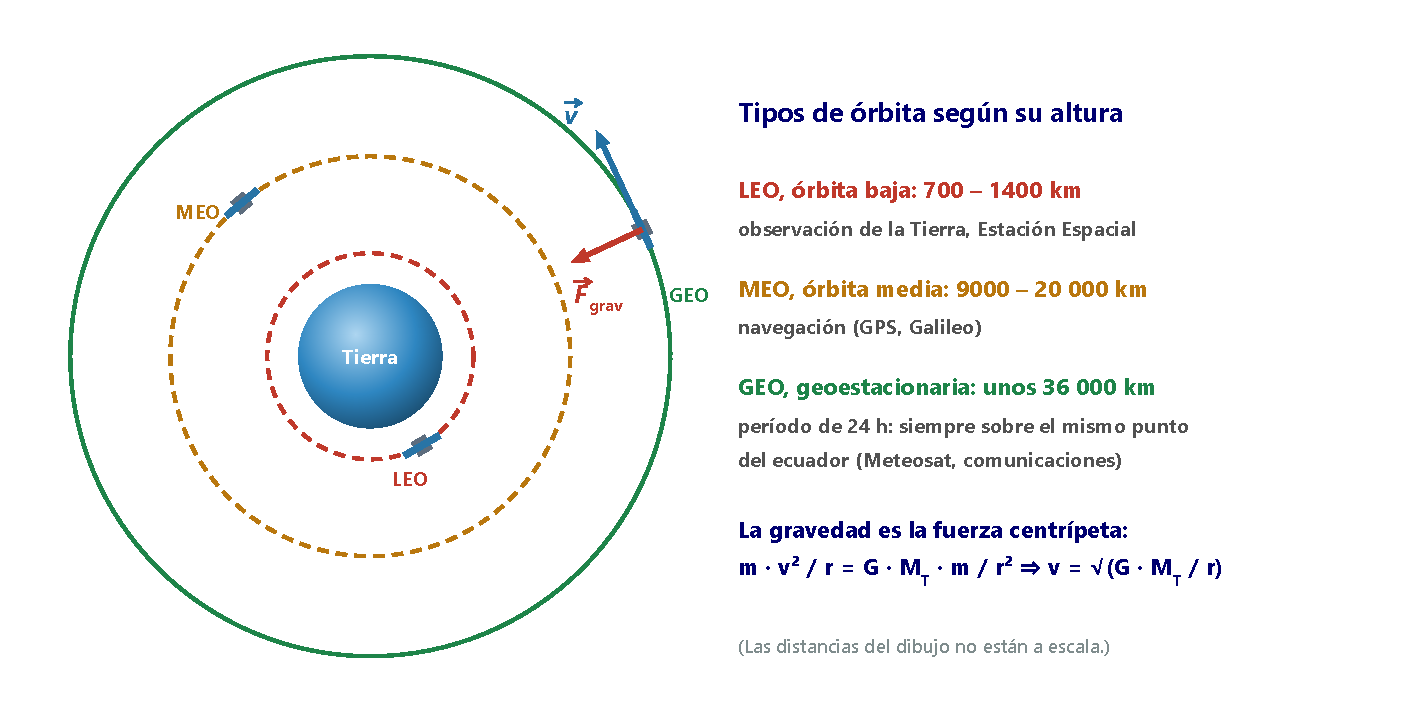
\includegraphics[width=0.95\textwidth]{images/UD9/orbitas_satelites}
    \caption{Tipos de órbita de los satélites artificiales.}
    \label{fig:orbitas_satelites}
\end{figure}

Como la Luna, un satélite está en órbita porque la atracción gravitatoria de la Tierra hace de fuerza centrípeta:
\[ m \cdot \frac{v^2}{r} = G \cdot \frac{M_T \cdot m}{r^2} \quad\Rightarrow\quad \boxed{v = \sqrt{G \cdot \frac{M_T}{r}}} \]
La velocidad orbital no depende de la masa del satélite, solo de la distancia \(r\) al centro de la Tierra: cuanto más lejos, más despacio. Y como \(v = 2\pi r / T\):
\[ \frac{4\pi^2 r^2}{T^2} = G \cdot \frac{M_T}{r} \quad\Rightarrow\quad \frac{T^2}{r^3} = \frac{4\pi^2}{G \cdot M_T} \quad\Rightarrow\quad T = \sqrt{\frac{4\pi^2 r^3}{G \cdot M_T}} \]
¡Es la tercera ley de Kepler! El cociente \(T^2/r^3\) es el mismo para todos los satélites de la Tierra. Newton demostró así que las leyes de Kepler son una consecuencia de la gravitación.

\begin{remark}
    \textbf{Basura espacial.} Se llama así a cualquier objeto artificial sin utilidad que orbita la Tierra: satélites viejos, restos de cohetes, fragmentos de choques\ldots{} Hay decenas de miles de objetos de más de \qty{10}{\cm}, cerca de un millón de fragmentos de más de \qty{1}{\cm} y miles de millones de partículas más pequeñas. A miles de kilómetros por hora, incluso un trozo pequeño puede destruir un satélite.
\end{remark}

\begin{example}
    ¿A qué velocidad gira un satélite en una órbita circular a \qty{30000}{\km} del centro de la Tierra?
    \[ v = \sqrt{G \cdot \frac{M_T}{r}} = \sqrt{\num{6.67e-11} \cdot \frac{\num{5.97e24}}{\num{3.0e7}}} = \textcolor{red}{\qty{3643}{\m\per\s}} \]
\end{example}

\begin{exercise}
    Calcula la aceleración centrípeta de un satélite que orbita a \qty{6570}{\km} del centro de la Tierra con un período de \qty{90}{\minute}.
    \begin{solu}
        \[ v = \frac{2\pi r}{T} = \frac{2\pi \cdot \num{6.57e6}}{\num{5400}} = \qty{7644}{\m\per\s} \qquad a_c = \frac{v^2}{r} = \frac{7644^2}{\num{6.57e6}} = \textcolor{red}{\qty{8.9}{\m\per\square\s}} \]
        Coincide con el valor de \(g\) a esa distancia: la aceleración centrípeta del satélite es la aceleración de la gravedad.
    \end{solu}
\end{exercise}

\begin{exercise}
    Calcula la velocidad de un satélite en una órbita circular a \qty{10000}{\km} del centro de la Tierra.
    \begin{solu}
        \[ v = \sqrt{G \cdot \frac{M_T}{r}} = \sqrt{\num{6.67e-11} \cdot \frac{\num{5.97e24}}{\num{1.0e7}}} = \textcolor{red}{\qty{6310}{\m\per\s}} \]
    \end{solu}
\end{exercise}

\subsection*{Actividades de consolidación: la síntesis newtoniana}

En estas actividades usa \(G = \qty{6.67e-11}{\newton\square\m\per\square\kg}\), \(M_T = \qty{5.97e24}{\kg}\) y \(R_T = \qty{6.37e6}{\m}\).

\begin{exercise}
    Calcula la aceleración de la gravedad a una altura sobre la superficie terrestre igual al radio de la Tierra.
    \begin{solu}
        La distancia al centro es \(2R_T = \qty{1.274e7}{\m}\):
        \[ g = \num{6.67e-11} \cdot \frac{\num{5.97e24}}{(\num{1.274e7})^2} = \textcolor{red}{\qty{2.45}{\m\per\square\s}} \]
        Al doblar la distancia al centro, \(g\) se divide entre cuatro.
    \end{solu}
\end{exercise}

\begin{exercise}
    ¿Cuánto pesa en la Luna (\(g_L = \qty{1.6}{\m\per\square\s}\)) una persona de \qty{80}{\kg}? ¿Y una piedra de \qty{1}{\kg}?
    \begin{solu}
        \(P = m \cdot g_L\): persona, \(80 \cdot \num{1.6} = \textcolor{red}{\qty{128}{\newton}}\); piedra, \(1 \cdot \num{1.6} = \textcolor{red}{\qty{1.6}{\newton}}\).
    \end{solu}
\end{exercise}

\begin{exercise}
    ¿A qué altura sobre la superficie terrestre se reduce \(g\) a la mitad?
    \begin{solu}
        \[ G \frac{M_T}{(R_T + h)^2} = \frac{1}{2} \cdot G \frac{M_T}{R_T^2} \quad\Rightarrow\quad (R_T + h)^2 = 2R_T^2 \quad\Rightarrow\quad h = (\sqrt{2} - 1) \cdot R_T = \textcolor{red}{\qty{2.64e6}{\m}} \]
        Unos \qty{2640}{\km}.
    \end{solu}
\end{exercise}

\begin{exercise}
    Calcula la velocidad de la Luna en su órbita y su período, sabiendo que está a \qty{380000}{\km} de la Tierra.
    \begin{solu}
        \[ v = \sqrt{G \frac{M_T}{r}} = \sqrt{\num{6.67e-11} \cdot \frac{\num{5.97e24}}{\num{3.8e8}}} = \textcolor{red}{\qty{1024}{\m\per\s}} \qquad T = \frac{2\pi r}{v} = \frac{2\pi \cdot \num{3.8e8}}{1024} = \textcolor{red}{\qty{2.33e6}{\s}} \]
        Unos 27 días.
    \end{solu}
\end{exercise}

\begin{exercise}
    Calcula a qué altura sobre la superficie y a qué velocidad orbita un satélite geoestacionario.
    \begin{solu}
        Un satélite geoestacionario gira en el plano del ecuador con un período de \(T = \qty{24}{\hour} = \qty{86400}{\s}\). De la expresión de la tercera ley:
        \[ r = \sqrt[3]{\frac{G \cdot M_T \cdot T^2}{4\pi^2}} = \sqrt[3]{\frac{\num{6.67e-11} \cdot \num{5.97e24} \cdot 86400^2}{4\pi^2}} = \qty{4.22e7}{\m} \]
        \[ h = r - R_T = \num{4.22e7} - \num{6.37e6} = \textcolor{red}{\qty{3.59e7}{\m}} \ (\text{unos } \qty{35900}{\km}) \qquad v = \sqrt{G \frac{M_T}{r}} = \textcolor{red}{\qty{3071}{\m\per\s}} \]
    \end{solu}
\end{exercise}

\begin{exercise}
    Calcula la velocidad, el período y la aceleración centrípeta de un satélite en órbita circular a \qty{2000}{\km} de altura.
    \begin{solu}
        \(r = \num{6.37e6} + \num{2.0e6} = \qty{8.37e6}{\m}\).
        \[ v = \sqrt{\num{6.67e-11} \cdot \frac{\num{5.97e24}}{\num{8.37e6}}} = \textcolor{red}{\qty{6897}{\m\per\s}} \qquad T = \frac{2\pi r}{v} = \textcolor{red}{\qty{7625}{\s}} \qquad a_c = \frac{v^2}{r} = \textcolor{red}{\qty{5.68}{\m\per\square\s}} \]
    \end{solu}
\end{exercise}

\begin{exercise}
    La masa de Júpiter es unas 318 veces la de la Tierra y su radio, unas 11 veces mayor. Calcula la gravedad en Júpiter (\(g_T = \qty{9.8}{\m\per\square\s}\)).
    \begin{solu}
        Dividimos las expresiones de \(g\) de los dos planetas; \(G\) se simplifica:
        \[ \frac{g_J}{g_T} = \frac{M_J}{M_T} \cdot \left(\frac{R_T}{R_J}\right)^2 = 318 \cdot \frac{1}{11^2} = \num{2.63} \quad\Rightarrow\quad g_J = \num{2.63} \cdot \num{9.8} = \textcolor{red}{\qty{25.8}{\m\per\square\s}} \]
    \end{solu}
\end{exercise}

\begin{exercise}
    ¿Cuánto vale la gravedad en un planeta con el mismo radio que la Tierra y la mitad de masa?
    \begin{solu}
        \(g\) es proporcional a la masa: \(g = \dfrac{\num{9.8}}{2} = \textcolor{red}{\qty{4.9}{\m\per\square\s}}\).
    \end{solu}
\end{exercise}

\begin{exercise}
    Calcula la gravedad en la superficie de Plutón, cuya masa es \qty{1.25e22}{\kg} y su radio, \qty{1188.3}{\km}.
    \begin{solu}
        \[ g = \num{6.67e-11} \cdot \frac{\num{1.25e22}}{(\num{1.1883e6})^2} = \textcolor{red}{\qty{0.59}{\m\per\square\s}} \]
    \end{solu}
\end{exercise}

%========================================================================================
\section[La fuerza eléctrica]{La fuerza eléctrica: una fuerza de la naturaleza}
%========================================================================================

Hasta comienzos del siglo \textsc{xx}, con el descubrimiento del electrón y los primeros modelos atómicos, no se explicó la naturaleza eléctrica de la materia. Los átomos tienen un núcleo con carga positiva (los protones) y, a su alrededor, electrones con carga negativa. Normalmente hay tantos protones como electrones y el átomo es \textbf{neutro}. Pero los electrones más externos pueden pasar de un cuerpo a otro: el cuerpo que \textbf{gana electrones} queda con carga \textbf{negativa}, y el que los \textbf{pierde}, con carga \textbf{positiva} (figura~\ref{fig:cargas_electricas}).

\begin{remark}
    En el siglo \textsc{xviii}, Benjamin Franklin demostró con su famosa cometa que los rayos son grandes descargas eléctricas. Como las descargas se dirigen hacia los objetos puntiagudos, inventó el \textbf{pararrayos}, que ha evitado muchas desgracias.
\end{remark}

\subsection{Unidades de la carga eléctrica}

La carga del electrón es la unidad natural de carga: la carga de cualquier cuerpo es siempre un \textbf{múltiplo entero} de ella. Como es muy pequeña, en el SI la carga, \(Q\), se mide en \textbf{culombios} (\unit{\coulomb}):
\[ e = \qty{1.6e-19}{\coulomb} \qquad\qquad \qty{1}{\coulomb} = \num{6.25e18}~\text{electrones} \]
En la práctica se usan submúltiplos como el microculombio: \(\qty{1}{\micro\coulomb} = \qty{1e-6}{\coulomb}\).

\subsection{Fuerzas entre cargas eléctricas. Ley de Coulomb}

\begin{figure}[H]
    \centering
    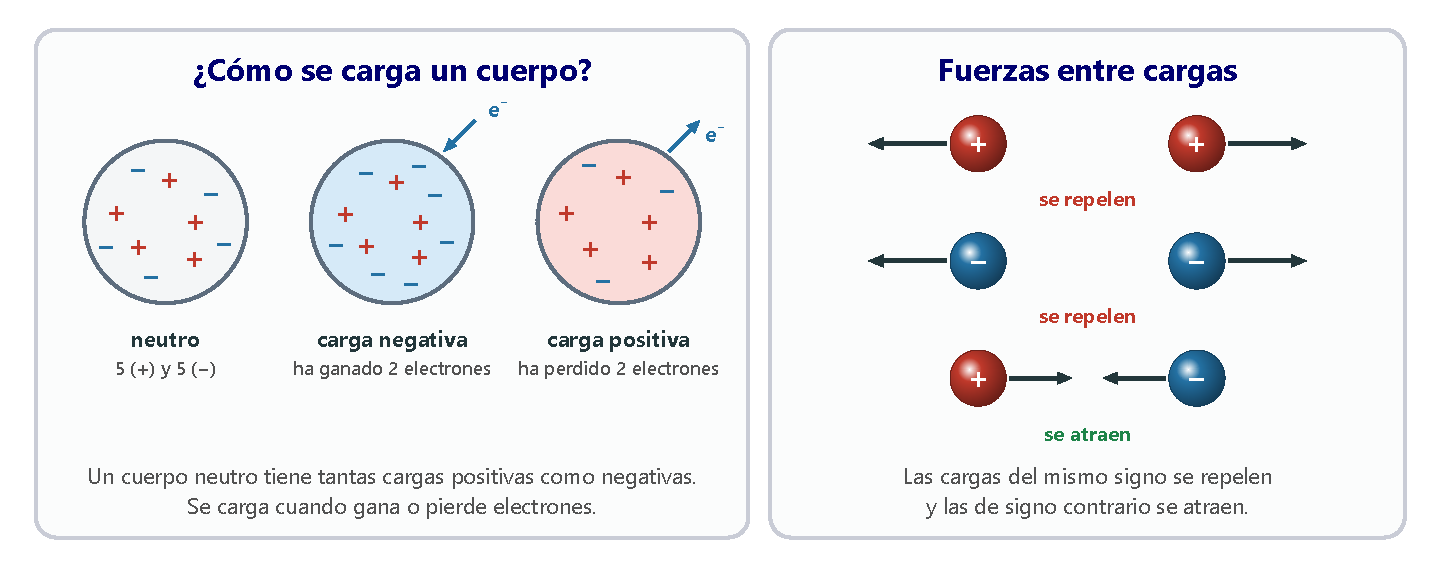
\includegraphics[width=\textwidth]{images/UD9/cargas_electricas}
    \caption{Cómo se carga un cuerpo y cómo actúan las fuerzas entre cargas.}
    \label{fig:cargas_electricas}
\end{figure}

En 1785, Charles-Augustin de \textbf{Coulomb} midió con una balanza de torsión las fuerzas entre cuerpos cargados. Las cargas del \textbf{mismo signo se repelen} y las de \textbf{signo contrario se atraen}, y el valor de la fuerza lo da la \textbf{ley de Coulomb}:

\begin{definition}[Ley de Coulomb]
    La fuerza con que se atraen o se repelen dos cargas puntuales \(Q\) y \(Q'\) es directamente proporcional al producto de sus valores e inversamente proporcional al cuadrado de la distancia \(r\) que las separa:
    \[ F = k \cdot \frac{Q \cdot Q'}{r^2} \qquad\qquad k = \qty{9e9}{\newton\square\m\per\square\coulomb} \ (\text{en el vacío o el aire}) \]
\end{definition}

Fíjate en el parecido con la ley de gravitación universal. Pero hay dos diferencias importantes: la fuerza eléctrica puede ser de \textbf{atracción o de repulsión}, y es \textbf{muchísimo más intensa}.

\begin{example}
    En un átomo de hidrógeno, el protón y el electrón están a \qty{5e-11}{\m}. Compara la fuerza eléctrica y la gravitatoria entre ellos (\(e = \qty{1.6e-19}{\coulomb}\), \(m_p = \qty{1.67e-27}{\kg}\), \(m_e = \qty{9.1e-31}{\kg}\)).
    \[ F_e = \num{9e9} \cdot \frac{(\num{1.6e-19})^2}{(\num{5e-11})^2} = \textcolor{red}{\qty{9.2e-8}{\newton}} \]
    \[ F_g = \num{6.67e-11} \cdot \frac{\num{1.67e-27} \cdot \num{9.1e-31}}{(\num{5e-11})^2} = \textcolor{red}{\qty{4.1e-47}{\newton}} \]
    La fuerza eléctrica es unas \(10^{39}\) veces mayor: dentro del átomo, la gravedad no cuenta.
\end{example}

\begin{exercise}
    ¿Puede existir un cuerpo cuya carga sea una fracción de la carga del electrón?
    \begin{solu}
        \textcolor{red}{No}. La carga del electrón es la unidad elemental: la carga de cualquier cuerpo es un número entero de veces esa carga.
    \end{solu}
\end{exercise}

\begin{exercise}
    Los dos protones del núcleo de helio están separados unos \qty{1e-15}{\m}. Calcula la fuerza eléctrica de repulsión entre ellos.
    \begin{solu}
        \[ F = k \cdot \frac{Q \cdot Q'}{r^2} = \num{9e9} \cdot \frac{(\num{1.6e-19})^2}{(\num{1e-15})^2} = \textcolor{red}{\qty{230}{\newton}} \]
        Es una fuerza enorme para dos partículas tan pequeñas: los protones se mantienen juntos gracias a otra fuerza todavía más intensa, la fuerza nuclear fuerte.
    \end{solu}
\end{exercise}

\subsection{El potencial eléctrico}

Imagina una carga positiva \(Q\) fija. Si queremos acercarle otra carga positiva, tenemos que vencer la repulsión, es decir, realizar un trabajo. Ese trabajo no se pierde: queda almacenado como \textbf{energía potencial electrostática}, \(E_p\).

\begin{definition}[Potencial eléctrico]
    El \textbf{potencial eléctrico}, \(V\), en un punto es la energía potencial que adquiere la unidad de carga positiva al traerla desde el infinito hasta ese punto. Es una magnitud escalar. A una distancia \(r\) de una carga \(Q\):
    \[ V = \frac{E_p}{q} = k \cdot \frac{Q}{r} \]
    Su unidad es el \textbf{voltio} (\unit{\volt}): \(\qty{1}{\volt} = \dfrac{\qty{1}{\joule}}{\qty{1}{\coulomb}}\).
\end{definition}

\subsection{Diferencia de potencial entre dos puntos}

Si en el punto A el potencial es \(V_A\) y en el punto B es \(V_B\), la \textbf{diferencia de potencial} entre ellos es \(V_A - V_B\), y también se mide en voltios. El trabajo que hay que realizar para llevar una carga \(q\) de A a B es:
\[ W_{A \to B} = q \cdot (V_B - V_A) \]
Si sale negativo, no hace falta hacer trabajo: la propia fuerza eléctrica lleva la carga de A a B.

\begin{example}
    Una carga \(Q = \qty{1}{\micro\coulomb}\) está en un punto O. Los puntos A y B están alineados con ella, a \qty{3}{\m} y \qty{6}{\m}. Calcula: a) el potencial en A y en B; b) el trabajo para llevar una carga de \qty{0.1}{\micro\coulomb} de A a B.

    a) \(V_A = k \dfrac{Q}{r_A} = \num{9e9} \cdot \dfrac{\num{1e-6}}{3} = \textcolor{red}{\qty{3000}{\volt}}\); \quad \(V_B = \num{9e9} \cdot \dfrac{\num{1e-6}}{6} = \textcolor{red}{\qty{1500}{\volt}}\)

    b) \(W = q \cdot (V_B - V_A) = \num{1e-7} \cdot (1500 - 3000) = \textcolor{red}{\qty{-1.5e-4}{\joule}}\). El signo negativo indica que la carga se aleja \textbf{sola}, empujada por la repulsión de \(Q\).
\end{example}

\begin{exercise}
    Una tormenta es una manifestación de las fuerzas eléctricas. Busca información sobre cómo se distribuyen las cargas en las nubes para que se formen los rayos.
    \begin{solu}
        Respuesta libre. Dentro de las nubes de tormenta, los choques entre cristales de hielo y gotas separan las cargas: la parte \textcolor{red}{superior} de la nube queda con carga \textcolor{red}{positiva} y la \textcolor{red}{inferior}, con carga \textcolor{red}{negativa}, que a su vez induce carga positiva en el suelo. Cuando la diferencia de potencial es enorme, el aire deja pasar una descarga: el \textbf{rayo}. El \textbf{relámpago} es su luz y el \textbf{trueno}, su sonido.
    \end{solu}
\end{exercise}

\subsection*{Actividades de consolidación: la fuerza eléctrica}

En estas actividades usa \(k = \qty{9e9}{\newton\square\m\per\square\coulomb}\).

\begin{exercise}
    Dos cuerpos con cargas de \qty{2.5}{\micro\coulomb} y \qty{3}{\micro\coulomb}, del mismo signo, están a \qty{5}{\cm}. ¿Se atraen o se repelen? ¿Con qué fuerza se atraerían si sus cargas fueran de signo contrario?
    \begin{solu}
        Como tienen el mismo signo, \textcolor{red}{se repelen}. Si fueran de signo contrario se atraerían con una fuerza del mismo módulo:
        \[ F = \num{9e9} \cdot \frac{\num{2.5e-6} \cdot \num{3e-6}}{(\num{0.05})^2} = \textcolor{red}{\qty{27}{\newton}} \]
    \end{solu}
\end{exercise}

\begin{exercise}
    ¿Cuál es el potencial en un punto si una carga de \qty{1}{\micro\coulomb} colocada en él tiene una energía potencial de \qty{0.001}{\joule}?
    \begin{solu}
        \(V = \dfrac{E_p}{q} = \dfrac{\num{0.001}}{\num{1e-6}} = \textcolor{red}{\qty{1000}{\volt}}\).
    \end{solu}
\end{exercise}

\begin{exercise}
    El potencial en un punto A es \qty{125}{\volt} y en un punto B, \qty{200}{\volt}. ¿Qué trabajo hay que realizar para llevar una carga de \qty{1}{\micro\coulomb} de A a B?
    \begin{solu}
        \(W = q \cdot (V_B - V_A) = \num{1e-6} \cdot (200 - 125) = \textcolor{red}{\qty{7.5e-5}{\joule}}\).
    \end{solu}
\end{exercise}

\begin{exercise}
    Una carga \(Q = \qty{2}{\micro\coulomb}\) está en un punto P. Los puntos A y B están alineados con ella, a \qty{2}{\m} y \qty{5}{\m}. Calcula:
    \begin{enumerate}[label=\alph*)]
        \item El potencial que crea \(Q\) en A y en B.
        \item El trabajo necesario para llevar una carga de \qty{-0.1}{\micro\coulomb} de A a B.
    \end{enumerate}
    \begin{solu}
        a) \(V_A = \num{9e9} \cdot \dfrac{\num{2e-6}}{2} = \textcolor{red}{\qty{9000}{\volt}}\); \(V_B = \num{9e9} \cdot \dfrac{\num{2e-6}}{5} = \textcolor{red}{\qty{3600}{\volt}}\).
        b) \(W = q \cdot (V_B - V_A) = (\num{-1e-7}) \cdot (3600 - 9000) = \textcolor{red}{\qty{5.4e-4}{\joule}}\). Es positivo: hay que hacer trabajo para alejar la carga negativa, porque \(Q\) la atrae.
    \end{solu}
\end{exercise}

%========================================================================================
\section[La fuerza magnética]{La fuerza magnética: una fuerza de la naturaleza}
%========================================================================================

La \textbf{magnetita} es un mineral que atrae el hierro, el cobalto, el níquel y algunas aleaciones de estos metales. Esta propiedad se llama \textbf{magnetismo}, y los cuerpos que la tienen son \textbf{imanes}.

\subsection{Clasificación de los imanes}

\begin{itemize}
    \item \textbf{Naturales y artificiales.} Un trozo de magnetita es un imán natural; un trozo de hierro o de acero imantado es un imán artificial.
    \item \textbf{Permanentes y temporales.} Si se ponen en contacto con un imán un trozo de hierro y uno de acero, los dos se imantan. Al separarlos, el acero sigue siendo un imán (\textbf{imán permanente}), pero el hierro deja de serlo (\textbf{imán temporal}).
\end{itemize}

\subsection{Propiedades de los imanes}

\begin{figure}[H]
    \centering
    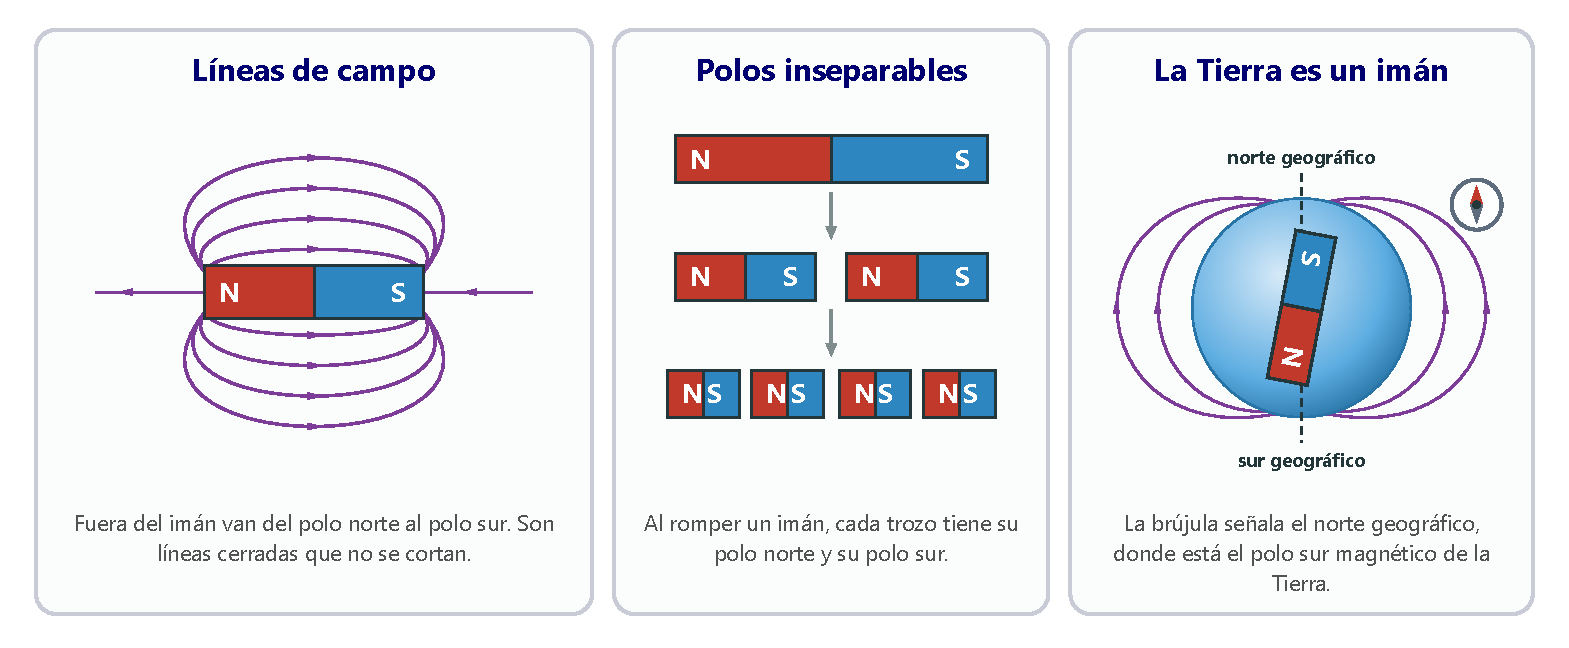
\includegraphics[width=\textwidth]{images/UD9/imanes}
    \caption{Líneas de campo de un imán de barra, imán roto y la Tierra como gran imán.}
    \label{fig:imanes}
\end{figure}

\begin{itemize}
    \item El magnetismo es más intenso en los extremos del imán, sus \textbf{polos}: el \textbf{polo norte} y el \textbf{polo sur}.
    \item \textbf{No se puede aislar un polo}: si rompemos un imán, cada trozo tiene su polo norte y su polo sur.
    \item Los polos del mismo nombre se \textbf{repelen} y los de distinto nombre se \textbf{atraen}.
\end{itemize}

Una \textbf{brújula} es una aguja imantada que gira libremente; uno de sus extremos se orienta hacia el norte geográfico. Por eso decimos que la Tierra es un gigantesco imán natural cuyo \textbf{polo sur magnético está cerca del polo norte geográfico} (el polo norte de la aguja es atraído por un polo sur). En realidad, el polo magnético está a unos \qty{1600}{\km} del polo geográfico, en el norte de Canadá, y se va desplazando con los años.

\paragraph{¿Qué son las líneas de campo magnético?} Si ponemos un papel sobre un imán y espolvoreamos limaduras de hierro, estas se ordenan formando unas líneas: las \textbf{líneas de campo magnético}. Son líneas \textbf{cerradas} que \textbf{no se cortan}; fuera del imán van del polo norte al polo sur, y por dentro, del sur al norte (figura~\ref{fig:imanes}).

\begin{marker}
    \textbf{Las auroras polares.} El Sol emite continuamente partículas con carga eléctrica (el \emph{viento solar}). El campo magnético terrestre las desvía y las conduce hacia las regiones polares. Allí chocan con los gases de la atmósfera, que emiten luz de colores: el oxígeno produce los tonos verdes y rojos, y el nitrógeno, los azules y violetas.
\end{marker}

\begin{exercise}
    Distingue entre imán temporal e imán permanente y entre imán natural e imán artificial.
    \begin{solu}
        Un imán \textcolor{red}{permanente} conserva la imantación mucho tiempo (por ejemplo, el acero); uno \textcolor{red}{temporal} solo es un imán mientras está en contacto con otro imán (por ejemplo, el hierro dulce). Un imán \textcolor{red}{natural} es un mineral que ya es magnético, como la magnetita; uno \textcolor{red}{artificial} es un material al que se ha imantado.
    \end{solu}
\end{exercise}

\begin{exercise}
    Explica por qué las auroras polares son un fenómeno magnético.
    \begin{solu}
        Las partículas cargadas del viento solar son \textcolor{red}{desviadas por el campo magnético terrestre}, que las guía hacia los polos siguiendo sus líneas de campo. Por eso las auroras solo se ven en las zonas cercanas a los polos, donde esas partículas chocan con los gases de la atmósfera y los hacen emitir luz.
    \end{solu}
\end{exercise}

%========================================================================================
\section[El electromagnetismo]{¿Qué relación hay entre electricidad y magnetismo? El electromagnetismo}
%========================================================================================

Durante siglos se pensó que electricidad y magnetismo eran fenómenos distintos. Dos experiencias del siglo \textsc{xix} demostraron que están íntimamente relacionados (figura~\ref{fig:oersted_faraday}).

\begin{figure}[H]
    \centering
    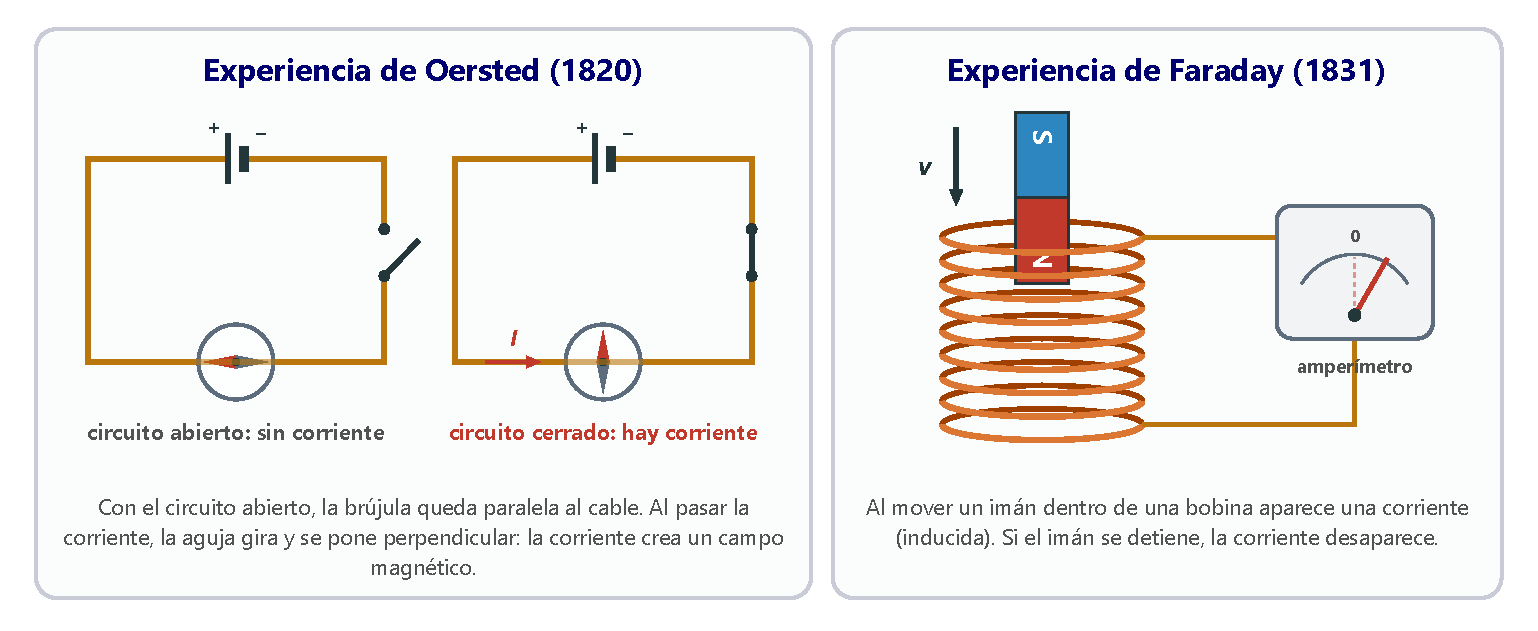
\includegraphics[width=\textwidth]{images/UD9/oersted_faraday}
    \caption{Las experiencias de Oersted y de Faraday.}
    \label{fig:oersted_faraday}
\end{figure}

\paragraph{La experiencia de Oersted.} En 1820, \textbf{Hans Christian Oersted} descubrió por casualidad que una corriente eléctrica desvía una brújula. Con el circuito abierto, la brújula situada bajo el cable se orienta de forma natural, paralela a él. Al cerrar el circuito, la aguja gira hasta ponerse perpendicular al cable, y si se invierte el sentido de la corriente, gira en sentido contrario. Conclusiones:
\begin{itemize}
    \item Una \textbf{carga eléctrica en reposo} solo produce fenómenos electrostáticos.
    \item Una \textbf{carga en movimiento} (una corriente) produce además un \textbf{campo magnético} a su alrededor.
\end{itemize}

\paragraph{La experiencia de Faraday.} En 1831, \textbf{Michael Faraday} comprobó lo contrario: un imán puede producir corriente eléctrica. Conectó una bobina a un medidor de corriente y observó que:
\begin{itemize}
    \item Al introducir un imán en la bobina, aparece una corriente; al sacarlo, aparece una corriente de sentido contrario.
    \item Si el imán está quieto dentro de la bobina, \textbf{no hay corriente}.
    \item Si se acerca el otro polo del imán, la corriente cambia de sentido.
\end{itemize}

\begin{definition}[Corriente inducida]
    Un \textbf{campo magnético variable} produce una corriente eléctrica en un circuito cercano, llamada \textbf{corriente inducida}. Existe mientras el campo magnético varía y es tanto mayor cuanto más rápida es la variación.
\end{definition}

En este fenómeno, la \textbf{inducción electromagnética}, se basan los generadores de las centrales eléctricas, las dinamos y las cocinas de inducción; y en el efecto descubierto por Oersted, los electroimanes y los motores eléctricos.

\begin{exercise}
    Describe las experiencias de Oersted y de Faraday. Ayúdate de esquemas o dibujos.
    \begin{solu}
        Respuesta libre basada en la figura~\ref{fig:oersted_faraday}. \textcolor{red}{Oersted}: una corriente eléctrica desvía una brújula, es decir, \textcolor{red}{la corriente crea un campo magnético}. \textcolor{red}{Faraday}: al mover un imán dentro de una bobina aparece una corriente, es decir, \textcolor{red}{un campo magnético variable crea una corriente eléctrica}.
    \end{solu}
\end{exercise}


%------------------------------------------------


    \chapterimage{images/portada_cabeceras/cabecera_UD10}
    \chapter{Fuerzas en los fluidos}

    %! Author = crist
%! Date = 25/10/2026

\spacing{1.3}
%----------------------------------------------------------------------------------------
%	UNIDAD 10: FUERZAS EN LOS FLUIDOS (4.º ESO)
%   Figuras: images/UD10/*.pdf (fuente HTML en images/UD10/html, SVG en images/UD10/svg)
%   Gráficas con pgfplots: estilo «grafica», definido al inicio de la UD7.
%   Unidades \atm y \mmHg: declaradas al inicio de la UD5.
%   Datos usados en toda la unidad: g = 9,8 m/s², ρ(agua) = 1000 kg/m³, ρ(agua de mar) = 1030 kg/m³,
%   1 atm = 760 mmHg = 1,013·10^5 Pa.
%----------------------------------------------------------------------------------------

% Mapa conceptual del tema (fuente en images/mapas_conceptuales/html/temas.js)
\begin{figure}[H]
    \centering
    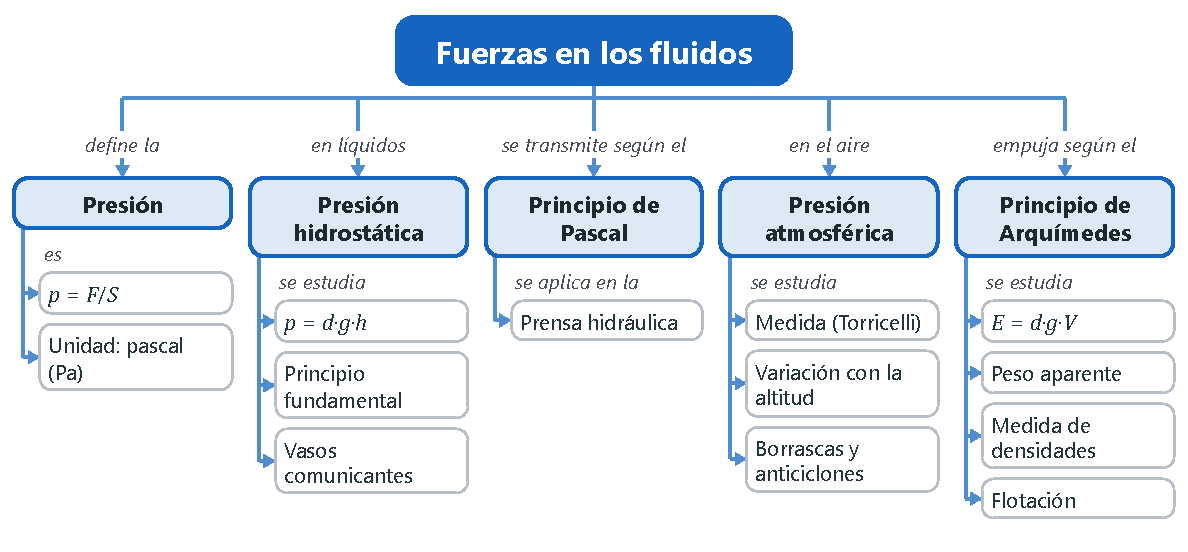
\includegraphics[width=\textwidth]{images/mapas_conceptuales/mapa_UD10}
\end{figure}

%========================================================================================
%\section*{Para empezar: la meteorología moderna}
%\addcontentsline{toc}{section}{Para empezar: la meteorología moderna}
%========================================================================================
%
%A comienzos del siglo \textsc{xx}, el noruego \textbf{Vilhelm Bjerknes} propuso tratar la predicción del tiempo como un problema de física: si se conoce con detalle el estado de la atmósfera en un momento dado (presión, temperatura, humedad, viento\ldots), las leyes de la física permiten calcular cómo va a evolucionar. Esa idea es la base de las predicciones actuales.
%
%Sin embargo, llevarla a la práctica no era fácil. Casi no había observaciones de las capas altas de la atmósfera, hasta que la aviación permitió tomar datos a gran altura. Además, los cálculos eran tan largos que el tiempo «pasaba» antes de terminarlos; el problema se resolvió con la llegada de los ordenadores. Desde el lanzamiento del primer satélite artificial, en 1957, la atmósfera también se observa desde el espacio.
%
%Una buena predicción no evita una tormenta, pero sí puede salvar vidas: avisar a tiempo permite preparar planes de emergencia ante inundaciones, temporales u olas de calor. Por eso la meteorología está relacionada con el \textbf{ODS 11} (\emph{Ciudades y comunidades sostenibles}), que busca reducir las muertes causadas por desastres naturales, y con el \textbf{ODS 13} (\emph{Acción por el clima}), que pide reforzar la capacidad de adaptación a los riesgos del clima.
%
%En esta unidad estudiaremos la \textbf{presión}, una magnitud imprescindible para entender los fluidos: por qué un buzo no puede bajar a cualquier profundidad, cómo funciona un gato hidráulico, qué mide un barómetro, qué significan las borrascas y los anticiclones de los mapas del tiempo y por qué flota un barco de acero.
%
%\begin{exercise}
%    ¿Qué idea de Bjerknes es la base de las predicciones meteorológicas actuales?
%    \begin{solu}
%        Tratar la predicción del tiempo como un \textcolor{red}{problema de física}: a partir del estado de la atmósfera en un instante (los «valores iniciales»), calcular con las leyes de la física cómo evolucionará.
%    \end{solu}
%\end{exercise}
%
%\begin{exercise}
%    ¿Qué dos dificultades había a comienzos del siglo \textsc{xx} para aplicar esa idea? ¿Cómo se resolvieron?
%    \begin{solu}
%        No había apenas \textcolor{red}{observaciones de las capas altas} de la atmósfera, lo que se resolvió con el desarrollo de la \textcolor{red}{aviación}; y los \textcolor{red}{cálculos eran muy largos}, lo que se resolvió con los \textcolor{red}{ordenadores}.
%    \end{solu}
%\end{exercise}
%
%\begin{exercise}
%    ¿Han sido útiles los satélites artificiales para la meteorología? Busca el nombre de algunos satélites meteorológicos y la altura a la que operan.
%    \begin{solu}
%        Sí, son \textcolor{red}{fundamentales}: observan continuamente grandes zonas de la atmósfera. Por ejemplo, los \textcolor{red}{Meteosat} europeos son geoestacionarios (a unos \qty{36000}{\km} de altura); otros, como los MetOp, son de órbita polar (a unos \qty{800}{\km}).
%    \end{solu}
%\end{exercise}
%
%\begin{exercise}
%    ¿Cómo puede ayudar la predicción meteorológica a reducir los daños de los desastres naturales? ¿Qué relación tiene con los ODS 11 y 13? Debatidlo en clase.
%    \begin{solu}
%        Respuesta libre. Prever con antelación una situación de emergencia permite \textcolor{red}{avisar a la población y preparar recursos}, lo que evita pérdidas de vidas y reduce daños en las ciudades (ODS 11) y mejora la adaptación a los riesgos del clima (ODS 13).
%    \end{solu}
%\end{exercise}

%========================================================================================
\section[Fuerza y superficie: la presión]{¿Existe una relación entre la intensidad de una fuerza y la superficie sobre la que actúa? La presión}
%========================================================================================

Si dejamos caer un prisma sobre una capa de plastilina o de arcilla, siempre desde la misma altura, la huella es más profunda cuanto \textbf{menor} es la cara sobre la que cae (figura~\ref{fig:presion_superficie}). Y si usamos prismas más pesados, las huellas son más profundas. El efecto de una fuerza depende, por tanto, de su intensidad y del tamaño de la superficie sobre la que actúa.

\begin{definition}[Presión]
    La \textbf{presión}, \(p\), es la fuerza que actúa perpendicularmente sobre cada unidad de superficie:
    \[ p = \frac{F}{S} \]
    donde \(F\) es el módulo de la fuerza y \(S\) el área de la superficie. En el SI se mide en \textbf{newton por metro cuadrado} (\unit{\newton\per\square\m}), unidad que se llama \textbf{pascal} (\unit{\pascal}): \(\qty{1}{\pascal} = \qty{1}{\newton\per\square\m}\).
\end{definition}

La presión es una \textbf{magnitud escalar}: en un punto tiene el mismo valor en todas las direcciones. Su ecuación de dimensiones es \([p] = \mathrm{M \cdot L^{-1} \cdot T^{-2}}\).

Con una superficie pequeña se consiguen presiones muy grandes aplicando fuerzas pequeñas. Por eso los cuchillos afilados cortan mejor que los romos y las puntas finas de los clavos, chinchetas y agujas penetran con facilidad. Al revés, para \emph{repartir} una fuerza se aumenta la superficie: las raquetas de nieve, los esquís o las orugas de un tractor evitan que se hundan en el terreno.

\begin{figure}[H]
    \centering
    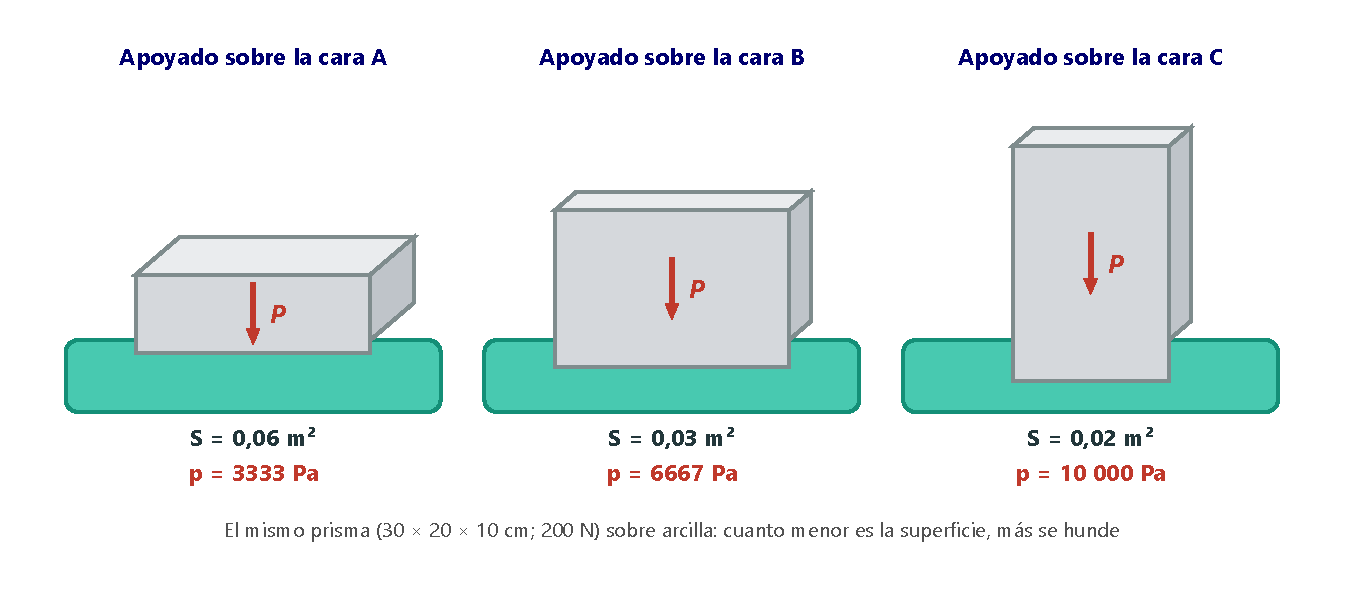
\includegraphics[width=\textwidth]{images/UD10/presion_superficie}
    \caption{Un mismo prisma ejerce más presión cuanto menor es la cara sobre la que se apoya.}
    \label{fig:presion_superficie}
\end{figure}

\begin{example}
    Un prisma rectangular de \(30 \times 20 \times 10\)~\unit{\cm} pesa \qty{200}{\newton}. Calcula la presión que ejerce sobre el suelo cuando se apoya sobre cada una de sus caras.

    Cara A (\(30 \times 20\)): \(S_A = \num{0.30} \cdot \num{0.20} = \qty{0.06}{\square\m}\); \quad \(p_A = \dfrac{200}{\num{0.06}} = \textcolor{red}{\qty{3333}{\pascal}}\).

    Cara B (\(30 \times 10\)): \(S_B = \num{0.30} \cdot \num{0.10} = \qty{0.03}{\square\m}\); \quad \(p_B = \dfrac{200}{\num{0.03}} = \textcolor{red}{\qty{6667}{\pascal}}\).

    Cara C (\(20 \times 10\)): \(S_C = \num{0.20} \cdot \num{0.10} = \qty{0.02}{\square\m}\); \quad \(p_C = \dfrac{200}{\num{0.02}} = \textcolor{red}{\qty{10000}{\pascal}}\).

    Al disminuir la superficie, aumenta la presión.
\end{example}

\begin{exercise}
    Escribe la ecuación de dimensiones de la presión a partir de su definición.
    \begin{solu}
        \([p] = \dfrac{[F]}{[S]} = \dfrac{\mathrm{M \cdot L \cdot T^{-2}}}{\mathrm{L^2}} = \textcolor{red}{\mathrm{M \cdot L^{-1} \cdot T^{-2}}}\).
    \end{solu}
\end{exercise}

\begin{exercise}
    Haz una lista de objetos que tengan filo o punta y explica para qué sirven.
    \begin{solu}
        Respuesta libre: cuchillos, tijeras, abrecartas, chinchetas, agujas, alfileres, clavos\ldots{} Todos sirven para cortar, clavar o penetrar en una superficie, porque su filo o su punta tienen una \textcolor{red}{superficie muy pequeña} y permiten ejercer \textcolor{red}{presiones muy elevadas} con fuerzas pequeñas.
    \end{solu}
\end{exercise}

\begin{exercise}
    Golpeamos con la misma fuerza dos clavos iguales: uno por la cabeza y otro por la punta (con la cabeza apoyada en la madera). ¿Cuál penetrará más fácilmente? ¿Por qué?
    \begin{solu}
        El que se golpea por la \textcolor{red}{cabeza}, porque la fuerza actúa sobre la madera a través de la punta, que tiene una superficie mucho menor: la \textcolor{red}{presión es mayor}.
    \end{solu}
\end{exercise}

\begin{exercise}
    Un prisma rectangular mide \(30 \times 20 \times 40\)~\unit{\cm} y pesa \qty{100}{\newton}. Calcula la presión que ejerce sobre una capa de arcilla al apoyarlo sobre cada una de sus caras.
    \begin{solu}
        Cara de \(30 \times 20\): \(p = \dfrac{100}{\num{0.3} \cdot \num{0.2}} = \textcolor{red}{\qty{1667}{\pascal}}\).
        Cara de \(30 \times 40\): \(p = \dfrac{100}{\num{0.3} \cdot \num{0.4}} = \textcolor{red}{\qty{833}{\pascal}}\).
        Cara de \(20 \times 40\): \(p = \dfrac{100}{\num{0.2} \cdot \num{0.4}} = \textcolor{red}{\qty{1250}{\pascal}}\).
    \end{solu}
\end{exercise}

\begin{exercise}
    Calcula la presión que ejerce una fuerza de \qty{100}{\newton} si se aplica sobre:
    \begin{enumerate}[label=\alph*)]
        \item Una superficie circular de \qty{20}{\cm} de radio.
        \item Una superficie cuadrada de \qty{20}{\cm} de lado.
    \end{enumerate}
    \begin{solu}
        a) \(S = \pi \cdot \num{0.20}^2 = \qty{0.126}{\square\m}\); \(p = \dfrac{100}{\num{0.126}} = \textcolor{red}{\qty{796}{\pascal}}\).
        b) \(S = \num{0.20}^2 = \qty{0.04}{\square\m}\); \(p = \dfrac{100}{\num{0.04}} = \textcolor{red}{\qty{2500}{\pascal}}\).
    \end{solu}
\end{exercise}

\begin{exercise}
    Un esquiador que pesa \qty{800}{\newton} se desliza con unos esquís de \qty{1200}{\square\cm} de superficie cada uno. ¿Qué presión ejerce sobre la nieve? ¿Y si estuviera de pie con unas botas de \qty{300}{\square\cm} cada una?
    \begin{solu}
        Con esquís: \(S = 2 \cdot \qty{0.12}{\square\m} = \qty{0.24}{\square\m}\); \(p = \dfrac{800}{\num{0.24}} = \textcolor{red}{\qty{3333}{\pascal}}\).
        Con botas: \(S = 2 \cdot \qty{0.03}{\square\m} = \qty{0.06}{\square\m}\); \(p = \dfrac{800}{\num{0.06}} = \textcolor{red}{\qty{13333}{\pascal}}\), cuatro veces más: por eso con botas se hunde en la nieve.
    \end{solu}
\end{exercise}

\subsection*{Actividades de consolidación: la presión}

\begin{exercise}
    Responde verdadero o falso y justifica tu respuesta:
    \begin{enumerate}[label=\alph*)]
        \item Un cuchillo afilado corta mejor que uno romo porque en su filo la presión es menor.
        \item El efecto de una fuerza depende del tamaño de la superficie sobre la que actúa.
        \item Para una misma fuerza, la presión es mayor cuanto mayor es la superficie sobre la que actúa.
    \end{enumerate}
    \begin{solu}
        a) \textcolor{red}{Falso}: corta mejor porque en su filo la presión es \emph{mayor}. b) \textcolor{red}{Verdadero}. c) \textcolor{red}{Falso}: la presión es mayor cuanto \emph{menor} es la superficie.
    \end{solu}
\end{exercise}

\begin{exercise}
    Una aguja de coser de \qty{e-6}{\square\m} de sección ejerce una presión de \qty{4e7}{\pascal} sobre la tela. ¿Con qué fuerza se ha empujado la aguja? ¿Qué presión ejercería si se duplicara la fuerza?
    \begin{solu}
        \(F = p \cdot S = \num{4e7} \cdot \num{e-6} = \textcolor{red}{\qty{40}{\newton}}\). Si la fuerza se duplica, también lo hace la presión: \(p = \textcolor{red}{\qty{8e7}{\pascal}}\).
    \end{solu}
\end{exercise}

\begin{exercise}
    La punta de un clavo tiene \qty{0.1}{\square\mm} de superficie. Con un martillo se golpea el clavo con una fuerza de \qty{150}{\newton}. ¿Qué presión ejerce el clavo sobre la madera?
    \begin{solu}
        \(S = \qty{0.1}{\square\mm} = \qty{e-7}{\square\m}\); \(p = \dfrac{150}{\num{e-7}} = \textcolor{red}{\qty{1.5e9}{\pascal}}\).
    \end{solu}
\end{exercise}

\begin{exercise}
    Tres prismas se apoyan en el suelo: A pesa \qty{200}{\newton} y su base mide \qty{4}{\square\m}; B pesa \qty{200}{\newton} y su base mide \qty{2}{\square\m}; C pesa \qty{400}{\newton} y su base mide \qty{2}{\square\m}. Calcula la presión que ejerce cada uno. ¿Qué relación de proporcionalidad hay entre la presión, la fuerza y la superficie?
    \begin{solu}
        \(p_A = \dfrac{200}{4} = \textcolor{red}{\qty{50}{\pascal}}\); \(p_B = \dfrac{200}{2} = \textcolor{red}{\qty{100}{\pascal}}\); \(p_C = \dfrac{400}{2} = \textcolor{red}{\qty{200}{\pascal}}\).
        La presión es \textcolor{red}{directamente proporcional a la fuerza} (de B a C se duplica la fuerza y se duplica la presión) e \textcolor{red}{inversamente proporcional a la superficie} (de A a B se reduce la superficie a la mitad y la presión se duplica).
    \end{solu}
\end{exercise}

\begin{exercise}
    Una maleta de \(1{,}0 \times 0{,}5 \times 0{,}2\)~\unit{\m} pesa \qty{200}{\newton}. Calcula la presión que ejerce sobre el suelo en estas posiciones: A, tumbada sobre su cara mayor; B, apoyada de canto sobre la cara de \(1{,}0 \times 0{,}2\)~\unit{\m}; C, de pie sobre la cara de \(0{,}5 \times 0{,}2\)~\unit{\m}. ¿En qué posición es mayor la presión? ¿En cuál es menor?
    \begin{solu}
        \(p_A = \dfrac{200}{\num{1.0} \cdot \num{0.5}} = \qty{400}{\pascal}\); \(p_B = \dfrac{200}{\num{1.0} \cdot \num{0.2}} = \qty{1000}{\pascal}\); \(p_C = \dfrac{200}{\num{0.5} \cdot \num{0.2}} = \qty{2000}{\pascal}\).
        La presión es \textcolor{red}{mayor en C} (menor superficie de apoyo) y \textcolor{red}{menor en A}.
    \end{solu}
\end{exercise}

\begin{exercise}
    Completa la tabla en tu cuaderno:
    \begin{center}
        % --- tabla antigua ---
        % \begin{tblr}{colspec={ccc}, hlines, vlines, row{1}={bg=ocre!85, fg=white, font=\bfseries}}
            % Fuerza (N) & Superficie & Presión (Pa) \\
            % 100 & \qty{1}{\square\mm} & \ldots \\
            % 100 & \qty{1}{\square\cm} & \ldots \\
            % 100 & \qty{1}{\square\m} & \ldots \\
        % \end{tblr}
        % --- tabla nueva ---
        \begin{tabular}{@{}ccc@{}}
            \toprule
            \textbf{Fuerza (N)} & \textbf{Superficie} & \textbf{Presión (Pa)} \\
            \midrule
            100 & \qty{1}{\square\mm} & \ldots \\[3pt]
            100 & \qty{1}{\square\cm} & \ldots \\[3pt]
            100 & \qty{1}{\square\m} & \ldots \\
            \bottomrule
        \end{tabular}
    \end{center}
    \begin{solu}
        \(\dfrac{100}{\num{e-6}} = \textcolor{red}{\qty{e8}{\pascal}}\); \(\dfrac{100}{\num{e-4}} = \textcolor{red}{\qty{e6}{\pascal}}\); \(\dfrac{100}{1} = \textcolor{red}{\qty{100}{\pascal}}\).
    \end{solu}
\end{exercise}

\begin{exercise}
    Dos personas de \qty{65}{\kg} están de pie en un terreno blando. Una lleva zapatos de tacón fino, de \qty{4}{\square\cm} de superficie cada tacón, y la otra zapatos de tacón ancho, de \qty{30}{\square\cm}. Sobre los tacones descansa el \qty{70}{\percent} del peso de cada persona.
    \begin{enumerate}[label=\alph*)]
        \item Calcula la presión que ejercen sobre el suelo los tacones de cada persona.
        \item Si el suelo aguanta como máximo \qty{5e4}{\pascal}, ¿se deformará bajo el peso de estas personas?
    \end{enumerate}
    \begin{solu}
        a) \(P = m \cdot g = 65 \cdot \num{9.8} = \qty{637}{\newton}\). Sobre los dos tacones descansan \(\num{0.70} \cdot 637 = \qty{446}{\newton}\), es decir, \qty{223}{\newton} sobre cada uno.
        Tacón fino: \(p = \dfrac{223}{\num{4e-4}} = \textcolor{red}{\qty{5.6e5}{\pascal}}\). Tacón ancho: \(p = \dfrac{223}{\num{3e-3}} = \textcolor{red}{\qty{7.4e4}{\pascal}}\).
        b) Las dos presiones son mayores que \qty{5e4}{\pascal}: el suelo \textcolor{red}{se deforma en los dos casos}, aunque mucho más con el tacón fino.
    \end{solu}
\end{exercise}

%========================================================================================
\section[La presión hidrostática]{¿Qué presión actúa en el interior de un fluido en reposo? La presión hidrostática}
%========================================================================================

Llamamos \textbf{fluidos} a los líquidos y a los gases, porque pueden fluir y adaptarse a la forma del recipiente. Un fluido en reposo ejerce fuerzas sobre las paredes del recipiente que lo contiene y sobre los cuerpos sumergidos en él, debidas a su propio peso. Además, cada capa del fluido soporta el peso de las capas que tiene encima.

\begin{definition}[Presión hidrostática]
    En el interior de un fluido en reposo existe una presión debida a su propio peso, que se llama \textbf{presión hidrostática}.
\end{definition}

\subsection{¿De qué factores depende la presión hidrostática?}

Con experiencias sencillas como las de la figura~\ref{fig:factores_presion} se comprueba que:
\begin{itemize}
    \item El fluido ejerce fuerzas \textbf{perpendiculares} a las superficies con las que está en contacto.
    \item La presión \textbf{aumenta con la profundidad}, medida desde la superficie libre del líquido.
    \item La presión \textbf{no depende de la forma del recipiente} ni de la cantidad de líquido, solo de la profundidad.
    \item En un punto, la presión es la \textbf{misma en todas las direcciones}.
    \item A la misma profundidad, la presión es mayor cuanto \textbf{mayor es la densidad} del líquido.
\end{itemize}

\begin{figure}[H]
    \centering
    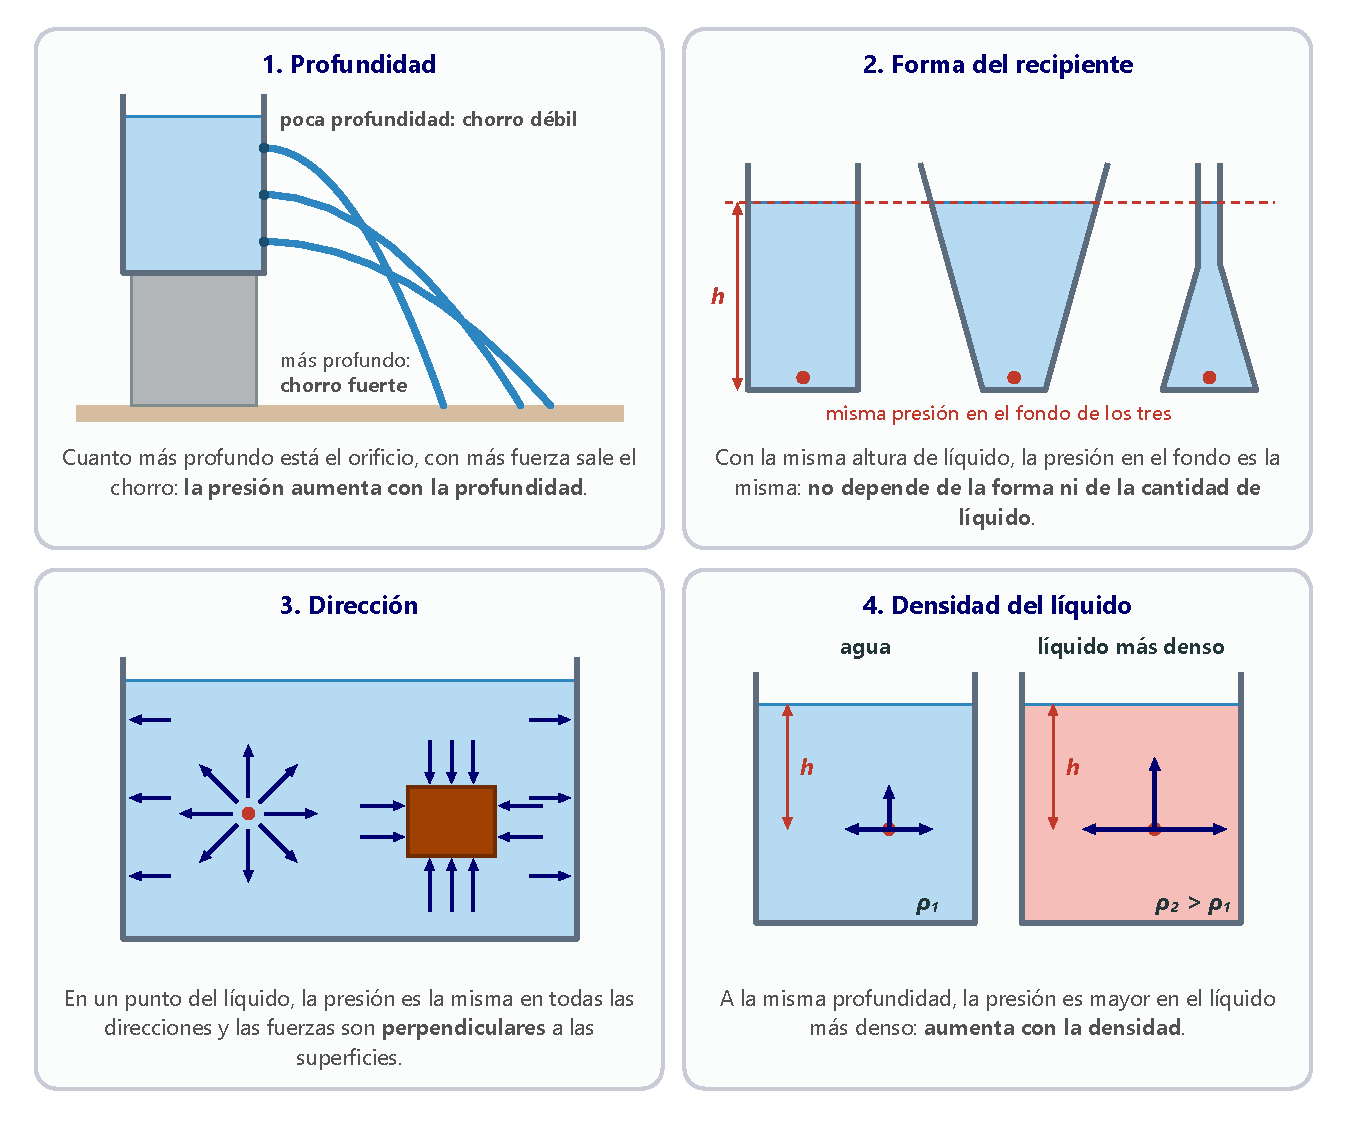
\includegraphics[width=\textwidth]{images/UD10/factores_presion}
    \caption{Factores de los que depende la presión en el interior de un líquido.}
    \label{fig:factores_presion}
\end{figure}

\subsection{¿Cómo se calcula la presión hidrostática?}

Para calcular la presión en un punto A situado a una profundidad \(h\), imaginamos una columna de líquido de base \(S\) que va desde A hasta la superficie libre (figura~\ref{fig:presion_hidrostatica}). La fuerza que actúa sobre la base es el peso de la columna:
\[ F = m \cdot g = \rho \cdot V \cdot g = \rho \cdot S \cdot h \cdot g \]
ya que la masa es \(m = \rho \cdot V\) y el volumen de la columna es \(V = S \cdot h\). Dividiendo entre la superficie:
\[ p = \frac{F}{S} = \frac{\rho \cdot S \cdot h \cdot g}{S} = \rho \cdot g \cdot h \]

\begin{definition}[Presión hidrostática]
    La presión hidrostática a una profundidad \(h\) bajo la superficie libre de un líquido en reposo es igual al producto de la densidad del líquido por la aceleración de la gravedad y por la profundidad:
    \[ p = \rho \cdot g \cdot h \]
\end{definition}

\begin{figure}[H]
    \centering
    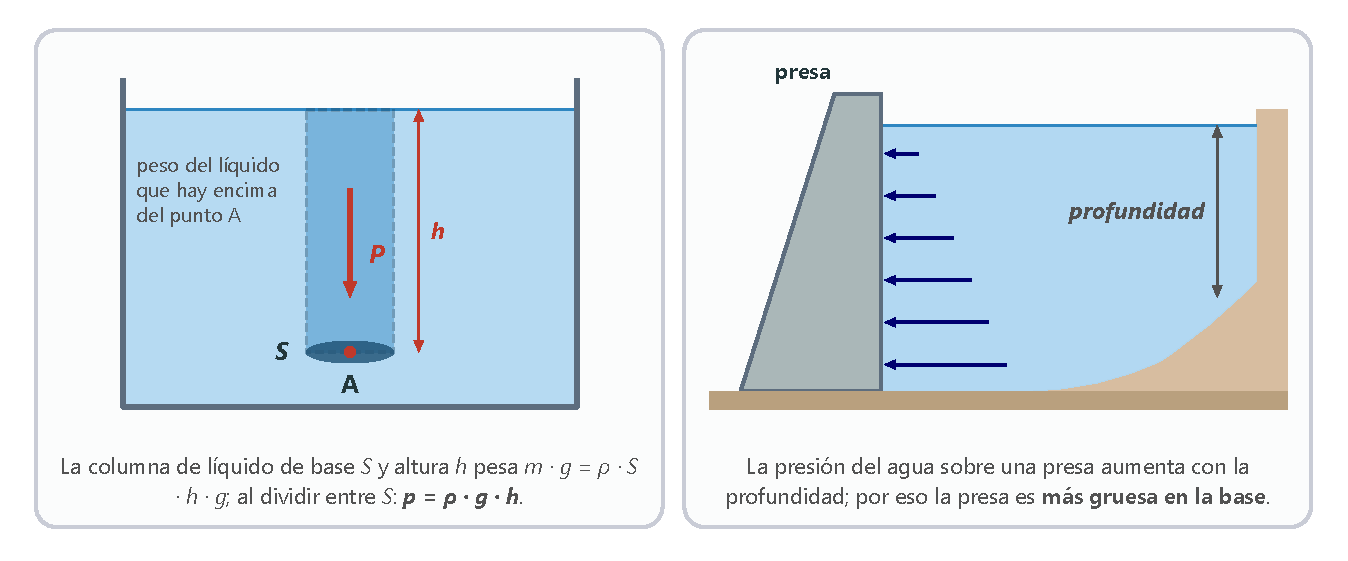
\includegraphics[width=\textwidth]{images/UD10/presion_hidrostatica}
    \caption{Cálculo de la presión hidrostática y presión del agua sobre una presa.}
    \label{fig:presion_hidrostatica}
\end{figure}

La presión hidrostática es \textbf{directamente proporcional} a la profundidad: su gráfica \(p\)--\(h\) es una recta que pasa por el origen, más inclinada cuanto más denso es el líquido.

\begin{center}
    \begin{tikzpicture}
        \begin{axis}[grafica, width=9cm, height=5.6cm, xlabel={profundidad, \(h\) (m)}, ylabel={\(p\) (kPa)}, xmin=0, xmax=10.5, ymin=0, ymax=110, legend pos=north west, legend style={font=\footnotesize}]
            \addplot[mark=none, domain=0:10, line width=1.4pt, color=blue!70!black] {1030*9.8*x/1000};
            \addlegendentry{agua de mar (\qty{1030}{\kg\per\cubic\m})}
            \addplot[mark=none, domain=0:10, line width=1.4pt, color=red!75!black] {800*9.8*x/1000};
            \addlegendentry{aceite (\qty{800}{\kg\per\cubic\m})}
        \end{axis}
    \end{tikzpicture}
\end{center}

\begin{example}
    En una bañera el agua alcanza \qty{35}{\cm} de altura. Calcula la presión hidrostática en el fondo y la fuerza con la que hay que tirar del tapón, circular y de \qty{5}{\cm} de diámetro, para vaciarla.

    \(p = \rho \cdot g \cdot h = 1000 \cdot \num{9.8} \cdot \num{0.35} = \textcolor{red}{\qty{3430}{\pascal}}\).

    La fuerza del agua sobre el tapón es perpendicular a él. Como \(S = \pi \cdot r^2 = \pi \cdot (\num{0.025})^2 = \qty{1.96e-3}{\square\m}\):
    \[ F = p \cdot S = 3430 \cdot \num{1.96e-3} = \textcolor{red}{\qty{6.7}{\newton}} \]
    Para sacar el tapón hay que tirar hacia arriba con una fuerza algo mayor que esta.
\end{example}

\begin{example}
    ¿Por qué el muro de una presa es más grueso en la base que en la parte de arriba?

    Porque la presión del agua \textcolor{red}{aumenta con la profundidad} (figura~\ref{fig:presion_hidrostatica}): la parte baja del muro soporta presiones mucho mayores y necesita más grosor de hormigón para resistirlas.
\end{example}

\begin{exercise}
    Dibuja en tu cuaderno un recipiente con agua y un cuerpo sumergido en ella, y representa las fuerzas que el líquido ejerce sobre las paredes del recipiente y sobre el cuerpo.
    \begin{solu}
        Las fuerzas son \textcolor{red}{perpendiculares} a las paredes y a las caras del cuerpo, dirigidas hacia ellas, y \textcolor{red}{más largas cuanto más profundo} está el punto (como en la figura~\ref{fig:factores_presion}).
    \end{solu}
\end{exercise}

\begin{exercise}
    ¿Qué presión hidrostática soporta un buzo sumergido en el mar a \qty{10}{\m} de profundidad?
    \begin{solu}
        \(p = \rho \cdot g \cdot h = 1030 \cdot \num{9.8} \cdot 10 = \textcolor{red}{\qty{100940}{\pascal}} \approx \qty{1}{\atm}\).
    \end{solu}
\end{exercise}

\begin{exercise}
    El embalse 1 es extenso y poco profundo (\qty{3}{\m}) y contiene más agua que el embalse 2, que es pequeño pero profundo (\qty{6}{\m}). ¿Por qué la presa del embalse 2 tiene que ser más gruesa que la del 1?
    \begin{solu}
        Porque la presión solo depende de la \textcolor{red}{profundidad}, no de la cantidad de agua. En el fondo del embalse 2 la presión es el doble que en el del 1, y su presa necesita \textcolor{red}{más grosor} para soportarla.
    \end{solu}
\end{exercise}

\subsection*{Actividades de consolidación: la presión hidrostática}

\begin{exercise}
    Copia y completa estas frases con las palabras: \emph{perpendicular, direcciones, mayor, mayor, sí depende, no depende}.

    «La presión en el interior de un líquido actúa en todas las \ldots{} y es \ldots{} a las paredes del recipiente. La presión es tanto \ldots{} cuanto \ldots{} es la profundidad; \ldots{} de la densidad del líquido, pero \ldots{} de la forma del recipiente».
    \begin{solu}
        «\ldots{} actúa en todas las \textcolor{red}{direcciones} y es \textcolor{red}{perpendicular} a las paredes del recipiente. La presión es tanto \textcolor{red}{mayor} cuanto \textcolor{red}{mayor} es la profundidad; \textcolor{red}{sí depende} de la densidad del líquido, pero \textcolor{red}{no depende} de la forma del recipiente».
    \end{solu}
\end{exercise}

\begin{exercise}
    ¿Qué presión ejerce sobre su base un prisma de hierro de \qty{20}{\cm} de altura y \qty{10}{\square\cm} de base? Dato: \(\rho_{\text{hierro}} = \qty{7800}{\kg\per\cubic\m}\). ¿Depende el resultado del área de la base?
    \begin{solu}
        \(p = \dfrac{P}{S} = \dfrac{\rho \cdot S \cdot h \cdot g}{S} = \rho \cdot g \cdot h = 7800 \cdot \num{9.8} \cdot \num{0.20} = \textcolor{red}{\qty{1.53e4}{\pascal}}\).
        \textcolor{red}{No depende del área} de la base, igual que la presión hidrostática no depende de la forma del recipiente.
    \end{solu}
\end{exercise}

\begin{exercise}
    Responde verdadero o falso y justifica tu respuesta:
    \begin{enumerate}[label=\alph*)]
        \item La presión en el interior de un líquido es mayor cuanto menor es su densidad.
        \item La presión es directamente proporcional a la anchura del recipiente.
        \item La presión es directamente proporcional a la profundidad.
        \item La presión en el interior de un líquido actúa en todas las direcciones.
    \end{enumerate}
    \begin{solu}
        a) \textcolor{red}{Falso}: es mayor cuanto mayor es la densidad. b) \textcolor{red}{Falso}: no depende de la anchura. c) \textcolor{red}{Verdadero}. d) \textcolor{red}{Verdadero}.
    \end{solu}
\end{exercise}

\begin{exercise}
    Tenemos cuatro recipientes de la misma altura llenos hasta arriba: A y B tienen la misma forma, pero A contiene agua y B mercurio; C y D contienen agua, pero D es mucho más estrecho que C. ¿Por qué la presión del mercurio sobre las paredes de B es mayor que la del agua sobre las paredes de A? ¿Por qué es la misma en C y en D?
    \begin{solu}
        En B la presión es mayor porque la \textcolor{red}{densidad del mercurio es mayor} que la del agua. En C y D es la misma porque contienen el mismo líquido y tienen la \textcolor{red}{misma profundidad}; la anchura no influye.
    \end{solu}
\end{exercise}

\begin{exercise}
    Toma un tubo de vidrio abierto por los dos extremos y tapa uno de ellos con una placa de plástico sujeta con un hilo tenso.
    \begin{enumerate}[label=\alph*)]
        \item Introduce el tubo en una cubeta con agua, con la placa hacia abajo. ¿Qué ocurre al soltar el hilo?
        \item Ahora echa agua dentro del tubo poco a poco. ¿Qué sucede cuando el nivel del agua del tubo alcanza el de la cubeta?
    \end{enumerate}
    \begin{solu}
        a) La placa \textcolor{red}{no se cae}: el agua de la cubeta la empuja hacia arriba (y lo hace en cualquier orientación del tubo).
        b) La placa \textcolor{red}{se desprende}, porque la presión del agua por dentro y por fuera es la misma y su propio peso la hace caer.
    \end{solu}
\end{exercise}

\begin{exercise}
    Calcula la presión en el fondo de un recipiente de \qty{76}{\cm} de profundidad cuando se llena de agua y cuando se llena de mercurio (\(\rho = \qty{13600}{\kg\per\cubic\m}\)).
    \begin{solu}
        Agua: \(p = 1000 \cdot \num{9.8} \cdot \num{0.76} = \textcolor{red}{\qty{7448}{\pascal}}\).
        Mercurio: \(p = 13600 \cdot \num{9.8} \cdot \num{0.76} = \textcolor{red}{\qty{1.013e5}{\pascal}}\), que es justo la presión atmosférica normal.
    \end{solu}
\end{exercise}

\begin{exercise}
    Una piscina tiene \qty{1}{\m} de profundidad en la zona menos profunda y \qty{2}{\m} en la más profunda. Calcula la presión del agua en el fondo de cada zona.
    \begin{solu}
        Zona profunda: \(p = 1000 \cdot \num{9.8} \cdot 2 = \textcolor{red}{\qty{19600}{\pascal}}\). Zona menos profunda: \(p = 1000 \cdot \num{9.8} \cdot 1 = \textcolor{red}{\qty{9800}{\pascal}}\).
    \end{solu}
\end{exercise}

\begin{exercise}
    Un batiscafo desciende en el océano hasta \qty{150}{\m} de profundidad. Si la densidad del agua es \qty{1040}{\kg\per\cubic\m}, calcula la presión hidrostática a esa profundidad y la fuerza que soporta una ventanilla circular de \qty{40}{\cm} de diámetro.
    \begin{solu}
        \(p = 1040 \cdot \num{9.8} \cdot 150 = \textcolor{red}{\qty{1.53e6}{\pascal}}\).
        \(S = \pi \cdot \num{0.20}^2 = \qty{0.126}{\square\m}\); \(F = p \cdot S = \num{1.53e6} \cdot \num{0.126} = \textcolor{red}{\qty{1.92e5}{\newton}}\) (como el peso de unas 20 toneladas).
    \end{solu}
\end{exercise}

\begin{exercise}
    Un submarino está sumergido a \qty{300}{\m} de profundidad en agua de mar. Calcula:
    \begin{enumerate}[label=\alph*)]
        \item La presión hidrostática sobre él, en pascales y en atmósferas.
        \item La fuerza que actúa sobre una de sus compuertas, de \qty{4.2}{\square\m}.
    \end{enumerate}
    \begin{solu}
        a) \(p = 1030 \cdot \num{9.8} \cdot 300 = \textcolor{red}{\qty{3.03e6}{\pascal}}\); \(\dfrac{\num{3.03e6}}{\num{1.013e5}} = \textcolor{red}{\qty{29.9}{\atm}}\).
        b) \(F = p \cdot S = \num{3.03e6} \cdot \num{4.2} = \textcolor{red}{\qty{1.27e7}{\newton}}\).
    \end{solu}
\end{exercise}

\begin{exercise}
    ¿Qué fuerza total soporta un buzo sumergido en el mar a \qty{8}{\m} de profundidad, si la superficie de su cuerpo es de \qty{150}{\square\dm}?
    \begin{solu}
        \(p = 1030 \cdot \num{9.8} \cdot 8 = \qty{80752}{\pascal}\). La superficie es \(\qty{150}{\square\dm} = \qty{1.5}{\square\m}\), así que
        \(F = p \cdot S = 80752 \cdot \num{1.5} = \textcolor{red}{\qty{1.21e5}{\newton}}\).
    \end{solu}
\end{exercise}

%========================================================================================
\section{Principio fundamental de la hidrostática}
%========================================================================================

Consideremos dos puntos A y B en el interior de un líquido en reposo, a las profundidades \(h_A\) y \(h_B\) (figura~\ref{fig:principio_fundamental}). Las presiones en ellos son \(p_A = \rho \cdot g \cdot h_A\) y \(p_B = \rho \cdot g \cdot h_B\), así que su diferencia es:
\[ p_A - p_B = \rho \cdot g \cdot (h_A - h_B) \]

\begin{definition}[Principio fundamental de la hidrostática]
    La \textbf{diferencia de presión entre dos puntos} de un fluido homogéneo en equilibrio es igual al producto de la densidad por la aceleración de la gravedad y por la diferencia de profundidad entre ellos:
    \[ \Delta p = \rho \cdot g \cdot \Delta h \]
\end{definition}

Una consecuencia importante: \textbf{todos los puntos de un líquido que están a la misma profundidad soportan la misma presión}, sea cual sea la forma del recipiente.

\begin{figure}[H]
    \centering
    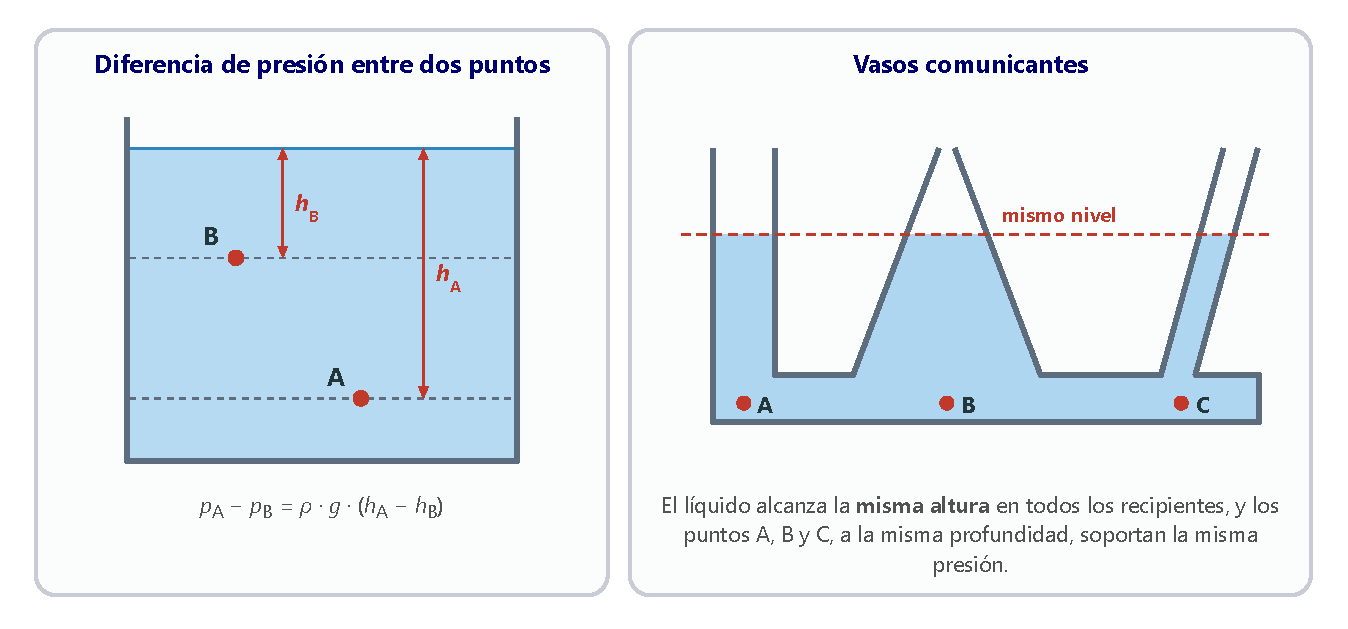
\includegraphics[width=\textwidth]{images/UD10/principio_fundamental}
    \caption{Principio fundamental de la hidrostática y vasos comunicantes.}
    \label{fig:principio_fundamental}
\end{figure}

\begin{example}
    Calcula la diferencia de presión entre dos puntos de un líquido de densidad \qty{1500}{\kg\per\cubic\m} situados a \qty{10}{\cm} y a \qty{30}{\cm} por debajo de la superficie libre.
    \[ p_A - p_B = \rho \cdot g \cdot (h_A - h_B) = 1500 \cdot \num{9.8} \cdot (\num{0.30} - \num{0.10}) = \textcolor{red}{\qty{2940}{\pascal}} \]
\end{example}

\subsection{¿Qué son los vasos comunicantes?}

Los \textbf{vasos comunicantes} son varios recipientes, de igual o distinta forma, abiertos por arriba y comunicados entre sí por la base. Si se vierte un líquido en uno de ellos, \textbf{alcanza la misma altura en todos} (figura~\ref{fig:principio_fundamental}).

Según el principio fundamental, la forma no influye: si el líquido estuviera más alto en un recipiente, la presión en su base sería mayor que en la de los demás y el líquido fluiría hasta igualar las alturas. Así funcionan el abastecimiento de agua de las ciudades desde depósitos elevados, los niveles de agua que usan los albañiles o las esclusas de los canales.

\begin{exercise}
    Una aplicación de los vasos comunicantes es el abastecimiento de agua a las ciudades.
    \begin{enumerate}[label=\alph*)]
        \item Busca información sobre cómo se abastece de agua una ciudad mediante depósitos.
        \item Justifica por qué el depósito debe estar a mayor altura que los edificios.
    \end{enumerate}
    \begin{solu}
        a) Respuesta libre. El agua se almacena en depósitos situados en lugares altos y llega a las casas por tuberías conectadas con ellos.
        b) La red de tuberías y el depósito forman unos \textcolor{red}{vasos comunicantes}: el agua tiende a alcanzar en las tuberías la misma altura que en el depósito. Para que llegue con presión suficiente a los pisos más altos, el depósito tiene que estar \textcolor{red}{por encima del edificio más alto}.
    \end{solu}
\end{exercise}

\begin{exercise}
    ¿Qué diferencia de presión hay entre dos puntos situados a \qty{1}{\m} y a \qty{10}{\m} por debajo de la superficie del agua?
    \begin{solu}
        \(\Delta p = \rho \cdot g \cdot \Delta h = 1000 \cdot \num{9.8} \cdot 9 = \textcolor{red}{\qty{88200}{\pascal}}\).
    \end{solu}
\end{exercise}

\subsection*{Actividades de consolidación: principio fundamental de la hidrostática}

\begin{exercise}
    ¿Qué diferencia de presión hay entre dos puntos situados a \qty{10}{\cm} y a \qty{35}{\cm} por debajo del nivel del agua?
    \begin{solu}
        \(\Delta p = 1000 \cdot \num{9.8} \cdot \num{0.25} = \textcolor{red}{\qty{2450}{\pascal}}\).
    \end{solu}
\end{exercise}

\begin{exercise}
    ¿A qué profundidad hay que sumergirse en un embalse para que la presión total que se soporta sea el doble que en la superficie? (En la superficie la presión es la atmosférica, \qty{1.013e5}{\pascal}).
    \begin{solu}
        La presión total será el doble cuando la presión hidrostática del agua sea igual a la atmosférica:
        \[ \num{1.013e5} = 1000 \cdot \num{9.8} \cdot h \quad\Rightarrow\quad h = \textcolor{red}{\qty{10.3}{\m}} \]
    \end{solu}
\end{exercise}

\begin{exercise}
    ¿Qué diferencia de presión hay entre dos puntos de un líquido de densidad \qty{1800}{\kg\per\cubic\m} separados por una distancia vertical de \qty{20}{\cm}?
    \begin{solu}
        \(\Delta p = 1800 \cdot \num{9.8} \cdot \num{0.20} = \textcolor{red}{\qty{3528}{\pascal}}\).
    \end{solu}
\end{exercise}

\begin{exercise}
    Si se ponen en comunicación vasijas de distintos tamaños y formas y se vierte un líquido en ellas, ¿cómo serán los niveles que alcanza el líquido?
    \begin{solu}
        El líquido alcanza el \textcolor{red}{mismo nivel en todas} las vasijas.
    \end{solu}
\end{exercise}

\begin{exercise}
    Un depósito cúbico de \qty{150}{\cm} de arista está lleno de agua. Calcula:
    \begin{enumerate}[label=\alph*)]
        \item La presión hidrostática en el fondo.
        \item La fuerza que ejerce el agua sobre el fondo.
        \item La presión en un punto situado a \qty{75}{\cm} de profundidad.
    \end{enumerate}
    \begin{solu}
        a) \(p = 1000 \cdot \num{9.8} \cdot \num{1.5} = \textcolor{red}{\qty{14700}{\pascal}}\).
        b) \(F = p \cdot S = 14700 \cdot \num{1.5}^2 = \textcolor{red}{\qty{33075}{\newton}}\) (coincide con el peso del agua del depósito).
        c) \(p = 1000 \cdot \num{9.8} \cdot \num{0.75} = \textcolor{red}{\qty{7350}{\pascal}}\).
    \end{solu}
\end{exercise}

%========================================================================================
\section{Principio de Pascal}
%========================================================================================

Si llenamos de agua una jeringa con un globo agujereado en la punta y empujamos el émbolo, el agua sale con la misma fuerza por todos los agujeros (figura~\ref{fig:pascal_prensa}). La presión que ejercemos con el émbolo se transmite a todo el líquido. En el siglo \textsc{xvii}, el científico francés \textbf{Blaise Pascal} lo enunció así:

\begin{definition}[Principio de Pascal]
    La presión ejercida en un punto de un \textbf{líquido incompresible} encerrado en un recipiente se transmite \textbf{por igual} a todos los puntos del líquido y a las paredes del recipiente, en todas las direcciones.
\end{definition}

\subsection{¿Qué aplicaciones tiene el principio de Pascal? La prensa hidráulica}

En el principio de Pascal se basan la prensa hidráulica, el gato y el elevador hidráulicos de los talleres, los frenos hidráulicos de los coches o las excavadoras.

La \textbf{prensa hidráulica} está formada por dos cilindros de secciones distintas, \(S_1\) (pequeña) y \(S_2\) (grande), unidos por un tubo y llenos de un líquido. Cada cilindro está cerrado por un émbolo. La presión que ejerce el émbolo pequeño se transmite sin variación al grande:
\[ p_1 = p_2 \quad\Rightarrow\quad \frac{F_1}{S_1} = \frac{F_2}{S_2} \quad\Rightarrow\quad F_2 = F_1 \cdot \frac{S_2}{S_1} \]
La fuerza que aparece en el émbolo grande es la aplicada en el pequeño \textbf{multiplicada por el cociente de las secciones}, \(S_2/S_1\). Cuanto mayor es la diferencia de tamaño de los émbolos, más eficaz es la prensa.

\begin{figure}[H]
    \centering
    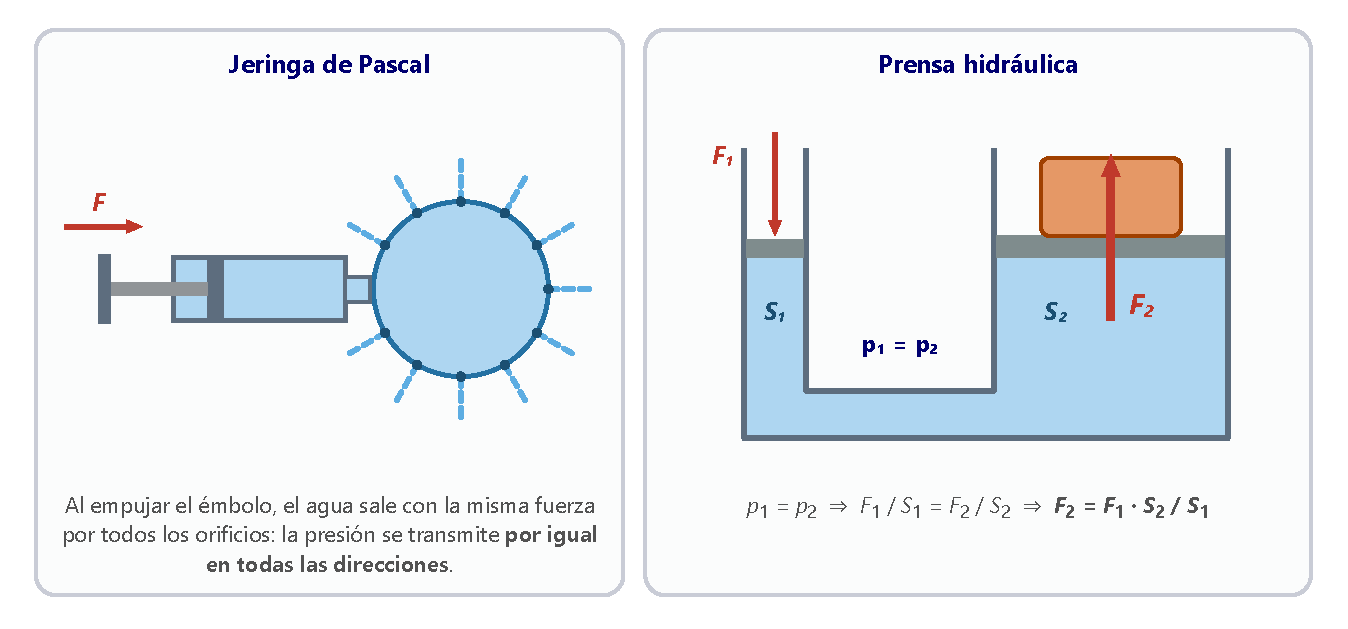
\includegraphics[width=\textwidth]{images/UD10/pascal_prensa}
    \caption{El principio de Pascal y la prensa hidráulica.}
    \label{fig:pascal_prensa}
\end{figure}

\begin{example}
    Los émbolos de una prensa hidráulica tienen \qty{1}{\cm} y \qty{10}{\cm} de radio. Sobre el pequeño se ejerce una fuerza de \qty{500}{\newton}. ¿Qué fuerza aparece en el grande?

    \(S_1 = \pi \cdot (\num{0.01})^2 = \qty{3.14e-4}{\square\m}\); \quad \(S_2 = \pi \cdot (\num{0.10})^2 = \qty{3.14e-2}{\square\m}\).
    \[ F_2 = F_1 \cdot \frac{S_2}{S_1} = 500 \cdot \frac{\num{3.14e-2}}{\num{3.14e-4}} = \textcolor{red}{\qty{5e4}{\newton}} \]
    Con \qty{500}{\newton} se pueden levantar unos \qty{5000}{\kg}: al multiplicar el radio por 10, la superficie (y la fuerza) se multiplica por 100.
\end{example}

\begin{exercise}
    ¿Qué superficie debe tener el émbolo grande de una prensa hidráulica para que, al ejercer \qty{20}{\newton} sobre el pequeño (de \qty{10}{\square\cm}), aparezca en el grande una fuerza de \qty{2000}{\newton}?
    \begin{solu}
        \(S_2 = S_1 \cdot \dfrac{F_2}{F_1} = 10 \cdot \dfrac{2000}{20} = \textcolor{red}{\qty{1000}{\square\cm}}\).
    \end{solu}
\end{exercise}

\subsection*{Actividades de consolidación: principio de Pascal}

\begin{exercise}
    Con una prensa hidráulica obtenemos una fuerza diez veces mayor que la que aplicamos. ¿Qué relación hay entre las secciones de los émbolos?
    \begin{solu}
        La sección del émbolo grande es \textcolor{red}{diez veces mayor} que la del pequeño.
    \end{solu}
\end{exercise}

\begin{exercise}
    La sección del émbolo grande de una prensa hidráulica es cien veces mayor que la del pequeño. ¿Qué fuerza actúa sobre el grande si sobre el pequeño se ejercen \qty{50}{\newton}?
    \begin{solu}
        \(F_2 = 50 \cdot 100 = \textcolor{red}{\qty{5000}{\newton}}\).
    \end{solu}
\end{exercise}

\begin{exercise}
    Un mecánico dice que su prensa hidráulica levanta camiones de hasta \qty{8000}{\kg}. La fuerza máxima que se puede aplicar sobre el émbolo pequeño es de \qty{2500}{\newton} y los diámetros de los émbolos son \qty{10}{\cm} y \qty{50}{\cm}. ¿Es cierto lo que dice?
    \begin{solu}
        Como \(S = \pi \cdot d^2/4\), el cociente de secciones es el cuadrado del cociente de diámetros: \(\dfrac{S_2}{S_1} = \left(\dfrac{50}{10}\right)^2 = 25\).
        \(F_2 = 2500 \cdot 25 = \qty{62500}{\newton}\), y el peso del camión es \(8000 \cdot \num{9.8} = \qty{78400}{\newton}\). \textcolor{red}{No es cierto}: como máximo levanta unos \qty{6400}{\kg}.
    \end{solu}
\end{exercise}

\begin{exercise}
    Queremos levantar con un elevador hidráulico una furgoneta que pesa \qty{20000}{\newton}. La sección del émbolo menor es de \qty{10}{\square\cm} y la del mayor, de \qty{140}{\square\cm}. ¿Qué fuerza hay que aplicar sobre el émbolo pequeño?
    \begin{solu}
        \(F_1 = F_2 \cdot \dfrac{S_1}{S_2} = 20000 \cdot \dfrac{10}{140} = \textcolor{red}{\qty{1429}{\newton}}\).
    \end{solu}
\end{exercise}

\begin{exercise}
    Busca información sobre cómo funcionan los frenos ABS de los coches y cómo deben usarlos los conductores. ¿El ABS aumenta o disminuye la distancia de frenado?
    \begin{solu}
        Respuesta libre. El ABS (\emph{sistema antibloqueo de frenos}) controla la presión del líquido de frenos para que las ruedas \textcolor{red}{no se bloqueen} al frenar: los neumáticos no pierden adherencia y el conductor puede frenar y girar a la vez. Hay que pisar el freno a fondo y mantenerlo pisado. En general, sobre todo en suelo mojado, \textcolor{red}{reduce la distancia de frenado} y evita derrapes.
    \end{solu}
\end{exercise}

%========================================================================================
\section[La presión atmosférica]{¿Ejerce la atmósfera presión sobre los cuerpos que están en su interior? La presión atmosférica}
%========================================================================================

Vivimos en el fondo de un «océano» de aire, la atmósfera, que tiene más de \qty{100}{\km} de espesor. Como cualquier fluido, el aire ejerce una presión sobre los cuerpos que hay en él, debida a su peso: es la \textbf{presión atmosférica}. Algunas experiencias cotidianas la ponen de manifiesto (figura~\ref{fig:presion_atmosferica}):
\begin{itemize}
    \item Al sorber con una pajita, sacamos el aire de su interior; la presión atmosférica, que actúa sobre la superficie del líquido del vaso, lo empuja hacia arriba por la pajita.
    \item Si llenamos un vaso de agua, lo tapamos con una cartulina y le damos la vuelta, el agua no cae: la presión atmosférica empuja la cartulina desde abajo.
    \item Las ventosas se quedan pegadas a una superficie lisa porque, al apretarlas, sale el aire de su interior y la presión atmosférica las aprieta desde fuera.
\end{itemize}

\begin{figure}[H]
    \centering
    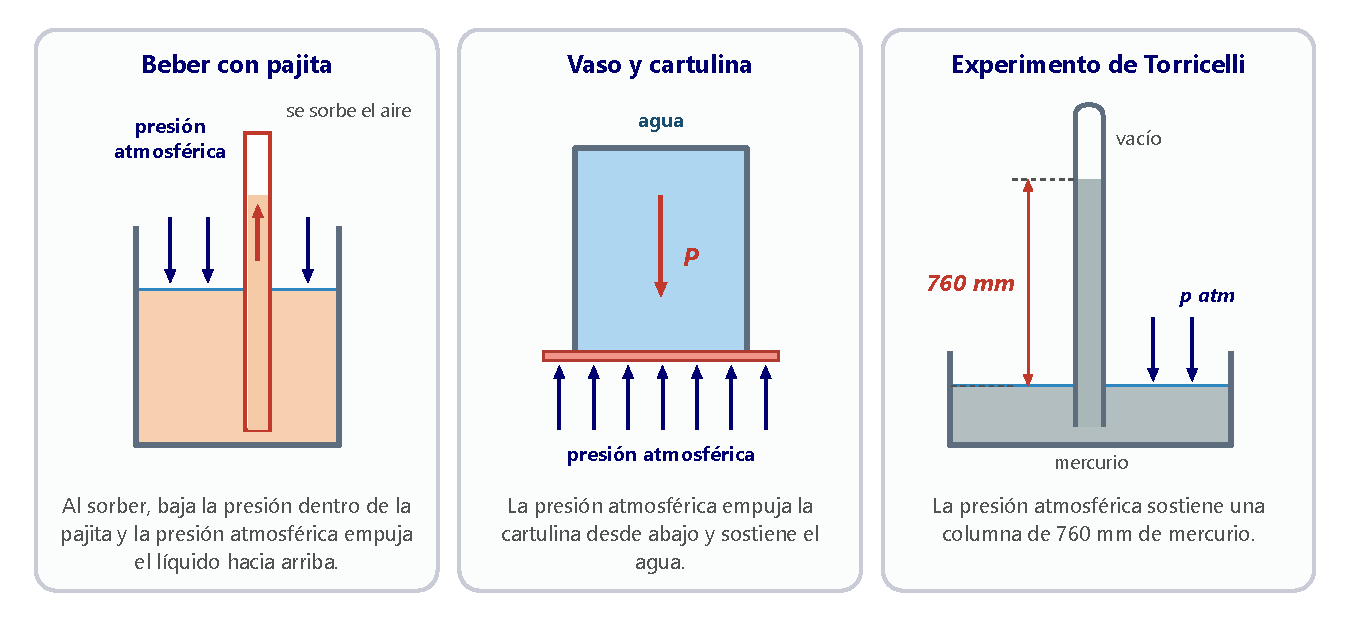
\includegraphics[width=\textwidth]{images/UD10/presion_atmosferica}
    \caption{Tres experiencias que muestran la presión atmosférica.}
    \label{fig:presion_atmosferica}
\end{figure}

\subsection{¿Cómo se mide la presión atmosférica?}

En 1643, el italiano \textbf{Evangelista Torricelli} llenó de mercurio un tubo de vidrio de \qty{1}{\m} de longitud, cerrado por un extremo. Tapó con el dedo el extremo abierto, le dio la vuelta y lo introdujo en una cubeta con mercurio. Al quitar el dedo, el mercurio del tubo bajó hasta quedar a \qty{760}{\mm} por encima del nivel de la cubeta, dejando vacío en la parte de arriba (figura~\ref{fig:presion_atmosferica}).

La columna no baja más porque la presión atmosférica, que actúa sobre el mercurio de la cubeta, la sostiene: la presión que ejerce la columna de mercurio es igual a la presión atmosférica.

\begin{definition}[Presión atmosférica normal]
    La presión que ejerce una columna de mercurio de \qty{760}{\mm} de altura se llama \textbf{presión atmosférica normal}, y para medirla se usa una unidad llamada \textbf{atmósfera} (\unit{\atm}):
    \[ \qty{1}{\atm} = \qty{760}{\mmHg} = \qty{1.013e5}{\pascal} \]
    La presión atmosférica se mide con un \textbf{barómetro}.
\end{definition}

Podemos comprobar la equivalencia con la presión hidrostática de la columna: \(p = \rho \cdot g \cdot h = 13600 \cdot \num{9.8} \cdot \num{0.760} = \qty{1.013e5}{\pascal}\).

La altura de la columna no depende de la longitud ni de la sección del tubo, ni de su inclinación: solo de la presión atmosférica del lugar.

\subsection{¿Qué relación hay entre la presión atmosférica y la altitud?}

Cuanto más subimos, menos aire tenemos encima y \textbf{menor es la presión atmosférica}. Además, el aire de las capas altas está menos comprimido y es menos denso, por lo que la presión no disminuye de forma proporcional a la altitud: cerca del nivel del mar hay que subir unos \qty{10}{\m} para que la presión baje \qty{1}{\mmHg}, pero a \qty{5000}{\m} de altitud hay que subir unos \qty{20}{\m}.

\begin{center}
    \begin{tikzpicture}
        \begin{axis}[grafica, width=10cm, height=6cm, xlabel={altitud (km)}, ylabel={presión (mmHg)}, xmin=0, xmax=12.5, ymin=0, ymax=800, xtick={0,2,...,12}]
            \addplot[mark=none, domain=0:12, samples=60, line width=1.4pt, color=red!75!black] {760*(1-0.022558*x)^5.256};
            \addplot[only marks, mark=*, mark size=2pt, color=blue!70!black] coordinates {(0,760) (5.5,380) (8.849,236)};
            \node[font=\scriptsize, anchor=west] at (axis cs:0.4,740) {nivel del mar: 760};
            \node[font=\scriptsize, anchor=south west] at (axis cs:5.6,382) {\qty{5500}{\m}: la mitad};
            \node[font=\scriptsize, anchor=south west] at (axis cs:8.9,238) {cima del Everest};
        \end{axis}
    \end{tikzpicture}
\end{center}

Por eso, a gran altura cuesta respirar (hay menos oxígeno en cada inspiración), el agua hierve a menos de \qty{100}{\degreeCelsius} y las cabinas de los aviones tienen que estar presurizadas. Los \textbf{altímetros} de los aviones son barómetros graduados en metros.

\subsection{Previsión del tiempo: borrascas y anticiclones}

En meteorología se usan como unidades de presión el \textbf{milibar} (mb) y el \textbf{hectopascal} (\unit{\hecto\pascal}), que son equivalentes: \(\qty{1}{\hecto\pascal} = \qty{100}{\pascal} = 1~\text{mb}\). El valor medio de la presión atmosférica a nivel del mar es de unos \qty{1013}{\hecto\pascal}; las presiones superiores se llaman \emph{altas} y las inferiores, \emph{bajas}.

\paragraph{¿Qué es un mapa meteorológico?} Es un mapa en el que se representan los valores de la presión atmosférica medidos a la vez en muchas estaciones meteorológicas; se usa para predecir el tiempo. Las \textbf{isobaras} son líneas que unen los puntos de igual presión, y suelen trazarse cada \qty{4}{\hecto\pascal}. Si están muy juntas, hay vientos fuertes; si están separadas, los vientos son suaves. Con una \textbf{A} se marcan los \textbf{anticiclones}, zonas de altas presiones, y con una \textbf{B}, las \textbf{borrascas}, zonas de bajas presiones (figura~\ref{fig:borrascas_anticiclones}).

\paragraph{¿Cómo se forman las borrascas y los anticiclones?} Se deben a las diferencias de temperatura en la atmósfera:
\begin{itemize}
    \item Si el aire está \textbf{frío}, es más denso y \textbf{desciende}, creando una zona de altas presiones: un \textbf{anticiclón}. Al llegar al suelo, el aire se separa (corrientes divergentes) y no se mezclan masas de aire distintas: el tiempo suele ser \textbf{bueno y estable}. En el hemisferio norte, el aire de un anticiclón gira en el sentido de las agujas del reloj.
    \item Si el aire está \textbf{caliente}, es menos denso y \textbf{asciende}, dejando debajo una zona de bajas presiones: una \textbf{borrasca}. El aire de los alrededores converge hacia ella, se mezclan masas de aire de distinto origen y, al subir, el vapor de agua se condensa: el tiempo suele ser \textbf{inestable}, con nubes y lluvias. En el hemisferio norte, el aire de una borrasca gira en sentido contrario al de las agujas del reloj.
\end{itemize}
En todos los casos el aire se desplaza desde las zonas de alta presión hasta las de baja presión: son las \textbf{corrientes de viento}. Las borrascas y los anticiclones no están quietos, sino que se desplazan y cambian de forma.

\begin{figure}[H]
    \centering
    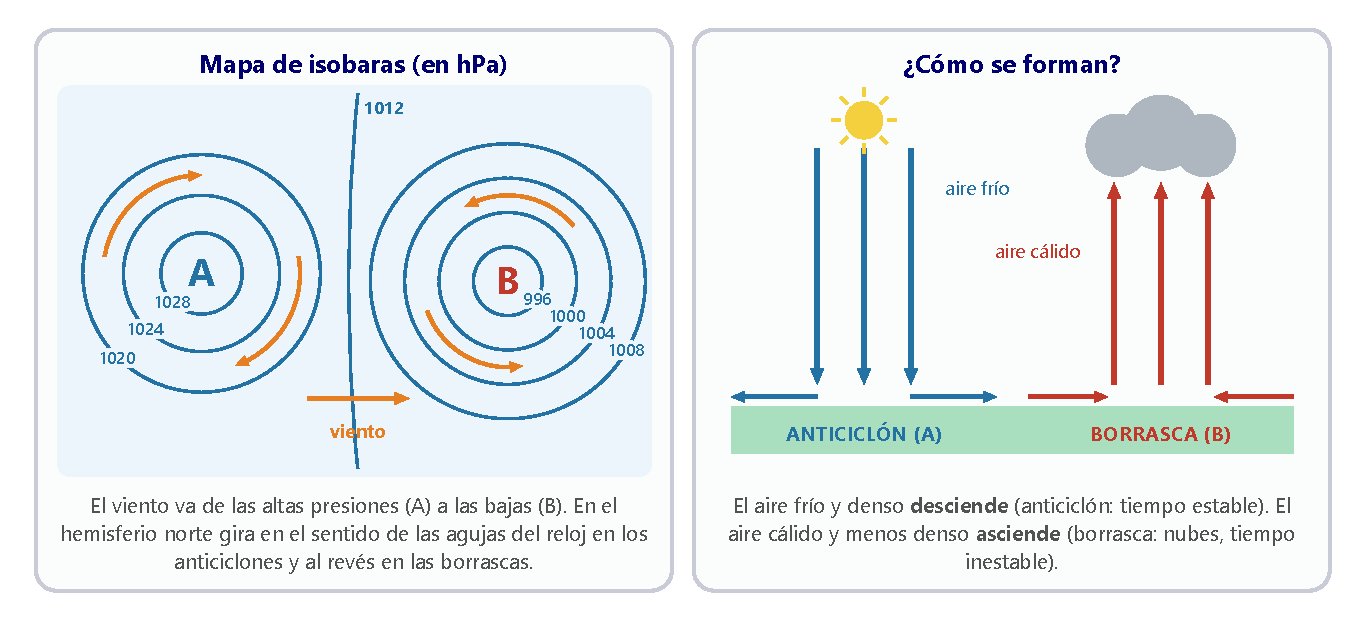
\includegraphics[width=\textwidth]{images/UD10/borrascas_anticiclones}
    \caption{Isobaras, anticiclones y borrascas.}
    \label{fig:borrascas_anticiclones}
\end{figure}

\paragraph{¿Qué diferencia hay entre un frente frío y uno cálido?} En la atmósfera hay \textbf{masas de aire frío}, más frías que la superficie sobre la que avanzan, y \textbf{masas de aire cálido}, más calientes. La zona de separación entre dos masas de aire distintas es una \textbf{superficie frontal}, y su intersección con el suelo es un \textbf{frente} (figura~\ref{fig:frentes}):
\begin{itemize}
    \item En un \textbf{frente frío}, el aire frío empuja al cálido y lo obliga a subir rápidamente; se forman nubes de gran desarrollo vertical y chubascos. En los mapas se dibuja con una línea de \textbf{triángulos} que apuntan en el sentido de avance.
    \item En un \textbf{frente cálido}, una masa de aire templado avanza y sube lentamente sobre el aire frío, que retrocede; se forman nubes extensas y lluvias débiles. Se dibuja con una línea de \textbf{semicírculos}.
\end{itemize}

\begin{figure}[H]
    \centering
    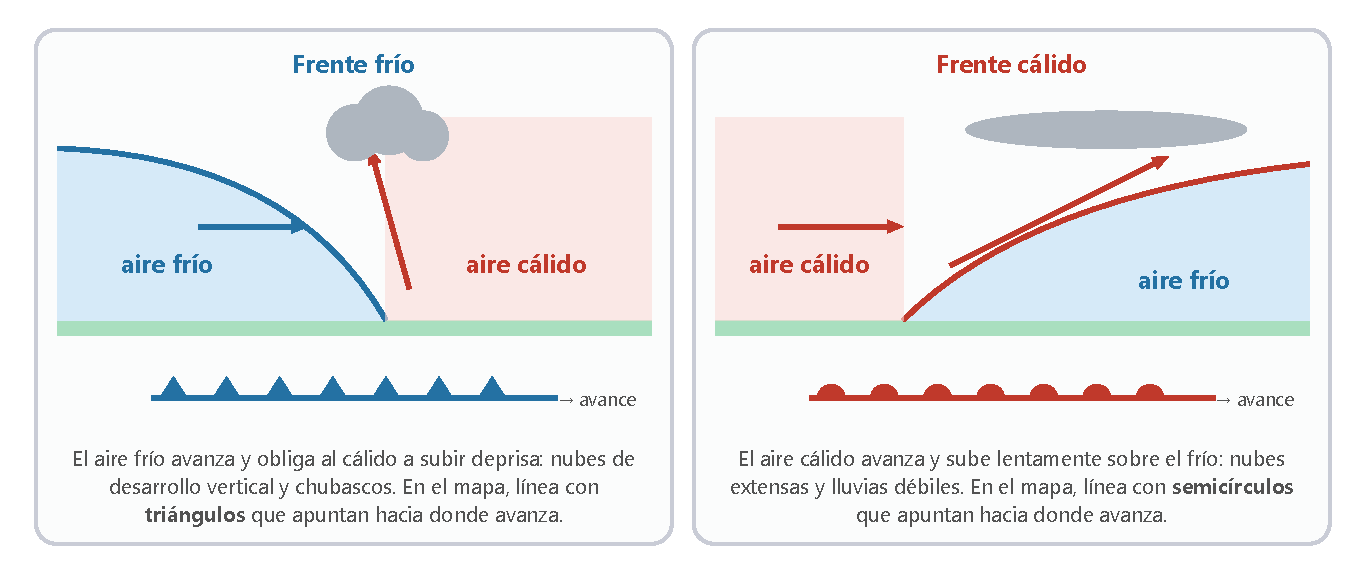
\includegraphics[width=\textwidth]{images/UD10/frentes}
    \caption{Frente frío y frente cálido, y sus símbolos en los mapas del tiempo.}
    \label{fig:frentes}
\end{figure}

\begin{exercise}
    La presión del aire dentro de un neumático es de \qty{1.25}{\atm}. Exprésala en milímetros de mercurio y en pascales.
    \begin{solu}
        \(\num{1.25}~\unit{\atm} \cdot \dfrac{\qty{760}{\mmHg}}{\qty{1}{\atm}} = \textcolor{red}{\qty{950}{\mmHg}}\); \quad \(\num{1.25}~\unit{\atm} \cdot \dfrac{\qty{1.013e5}{\pascal}}{\qty{1}{\atm}} = \textcolor{red}{\qty{1.27e5}{\pascal}}\).
    \end{solu}
\end{exercise}

\begin{exercise}
    ¿Por qué las cabinas de los aviones están selladas y presurizadas?
    \begin{solu}
        Porque a la altura a la que vuelan los aviones (unos \qty{10}{\km}) la \textcolor{red}{presión atmosférica es muy baja}, alrededor de una cuarta parte de la del nivel del mar, y no podríamos respirar bien. La cabina mantiene dentro una \textcolor{red}{presión mucho mayor} que la exterior, parecida a la que hay a unos \qty{2000}{\m} de altitud.
    \end{solu}
\end{exercise}

\begin{exercise}
    Un barómetro marca \qty{745}{\mmHg} en una localidad costera. ¿Hay una borrasca o un anticiclón sobre ella? ¿Qué tiempo cabe esperar?
    \begin{solu}
        Marca menos de \qty{760}{\mmHg} (\(745 \cdot \num{1.333} \approx \qty{993}{\hecto\pascal}\), por debajo de \qty{1013}{\hecto\pascal}): hay una \textcolor{red}{borrasca}, y cabe esperar \textcolor{red}{tiempo inestable}, con nubes y probablemente lluvia.
    \end{solu}
\end{exercise}

\begin{exercise}
    En un mapa del tiempo, la isobara más exterior que rodea un anticiclón es de \qty{1016}{\hecto\pascal}, y la más exterior que rodea una borrasca es de \qty{1004}{\hecto\pascal}. Si en el interior de cada uno hay dos isobaras más, trazadas cada \qty{4}{\hecto\pascal}, ¿qué valores tienen?
    \begin{solu}
        En el anticiclón la presión aumenta hacia el centro: \textcolor{red}{\qty{1020}{\hecto\pascal} y \qty{1024}{\hecto\pascal}}. En la borrasca disminuye hacia el centro: \textcolor{red}{\qty{1000}{\hecto\pascal} y \qty{996}{\hecto\pascal}}.
    \end{solu}
\end{exercise}

\subsection*{Actividades de consolidación: la presión atmosférica}

\begin{exercise}
    Asocia cada concepto con sus características (un concepto puede tener varias):

    \textbf{Conceptos:} a) presión atmosférica; b) isobaras; c) anticiclones; d) borrascas; e) corrientes de viento; f) frente frío; g) frente cálido.

    \textbf{Características:} 1. Línea con semicírculos. 2. Se mide con un barómetro. 3. Línea con triángulos. 4. Se expresa en atm, mmHg y Pa. 5. Líneas que unen puntos de igual presión. 6. Disminuye con la altitud. 7. Zonas de baja presión. 8. Zonas de alta presión. 9. Tiempo estable. 10. Tiempo inestable. 11. El aire va de las altas a las bajas presiones.
    \begin{solu}
        a) \textcolor{red}{2, 4 y 6}; b) \textcolor{red}{5}; c) \textcolor{red}{8 y 9}; d) \textcolor{red}{7 y 10}; e) \textcolor{red}{11}; f) \textcolor{red}{3}; g) \textcolor{red}{1}.
    \end{solu}
\end{exercise}

\begin{exercise}
    ¿Se puede usar un barómetro para calcular la altura de una montaña? Busca información sobre cómo funciona un altímetro.
    \begin{solu}
        \textcolor{red}{Sí}, porque la presión atmosférica disminuye con la altitud de forma conocida. Un \textcolor{red}{altímetro} es un barómetro graduado en metros: mide la presión y la convierte en la diferencia de altitud respecto a un lugar de referencia, normalmente el nivel del mar.
    \end{solu}
\end{exercise}

\begin{exercise}
    Si en el experimento de Torricelli se usara agua en lugar de mercurio, ¿qué altura alcanzaría el agua en el tubo?
    \begin{solu}
        \(\num{1.013e5} = 1000 \cdot \num{9.8} \cdot h \Rightarrow h = \textcolor{red}{\qty{10.3}{\m}}\). Haría falta un tubo de más de diez metros: por eso se usa mercurio, que es 13,6 veces más denso.
    \end{solu}
\end{exercise}

\begin{exercise}
    Si la densidad del aire fuera constante e igual a \qty{1.2}{\kg\per\cubic\m}, ¿qué altura tendría que tener la atmósfera para ejercer una presión de \qty{1.013e5}{\pascal}?
    \begin{solu}
        \(\num{1.013e5} = \num{1.2} \cdot \num{9.8} \cdot h \Rightarrow h = \textcolor{red}{\qty{8614}{\m}}\). La atmósfera real es mucho más alta porque su densidad disminuye con la altitud.
    \end{solu}
\end{exercise}

\begin{exercise}
    En una cubeta con mercurio se colocan tres tubos de un metro, cerrados por arriba y llenos de mercurio: uno vertical, otro inclinado y otro más ancho. ¿A qué altura vertical sobre el nivel de la cubeta quedará el mercurio en cada uno? ¿Por qué?
    \begin{solu}
        En los tres, a \textcolor{red}{\qty{760}{\mm}} de altura vertical (a nivel del mar). La presión atmosférica sobre la cubeta sostiene una columna cuya altura vertical \textcolor{red}{no depende de la forma, la sección ni la inclinación} del tubo (en el inclinado, el mercurio recorre más longitud de tubo, pero llega a la misma altura).
    \end{solu}
\end{exercise}

\begin{exercise}
    Una persona con una superficie corporal de \qty{1.5}{\square\m} soporta, por la presión atmosférica, una fuerza equivalente al peso de unas 15 toneladas. ¿Qué fuerza ejerce la atmósfera sobre una niña de \qty{1.25}{\square\m} de superficie corporal? ¿Por qué no nos aplasta?
    \begin{solu}
        \(F = p \cdot S = \num{1.013e5} \cdot \num{1.25} = \textcolor{red}{\qty{1.27e5}{\newton}}\), como el peso de unas 13 toneladas.
        No nos aplasta porque los fluidos de nuestro cuerpo están a una \textcolor{red}{presión igual}, que empuja hacia fuera y la equilibra.
    \end{solu}
\end{exercise}

\begin{exercise}
    En 1654, Otto von Guericke unió con grasa dos semiesferas de cobre en Magdeburgo y extrajo el aire de su interior: ni siquiera dos tiros de caballos consiguieron separarlas. Busca información sobre este experimento y explica por qué ocurre.
    \begin{solu}
        Respuesta libre. Al extraer el aire, dentro de las semiesferas casi no hay presión, mientras que por fuera actúa la \textcolor{red}{presión atmosférica}, que las aprieta una contra otra con una fuerza enorme (con semiesferas de unos \qty{50}{\cm} de diámetro, unos \qty{2e4}{\newton}).
    \end{solu}
\end{exercise}

\begin{exercise}
    Explica la diferencia entre un frente frío y uno cálido. Dibuja en tu cuaderno el símbolo de cada uno, indicando hacia dónde avanza y dónde están las masas de aire frío y cálido.
    \begin{solu}
        En un \textcolor{red}{frente frío} el aire frío avanza y levanta bruscamente al cálido; se dibuja con \textcolor{red}{triángulos} que apuntan hacia el aire cálido, que es hacia donde avanza. En un \textcolor{red}{frente cálido} el aire cálido avanza y sube lentamente sobre el frío; se dibuja con \textcolor{red}{semicírculos} que apuntan hacia el aire frío. En los dos casos, la masa que avanza está detrás de la línea (figura~\ref{fig:frentes}).
    \end{solu}
\end{exercise}

%========================================================================================
\section[Fuerzas de empuje. Principio de Arquímedes]{Fuerzas de empuje. Principio de Arquímedes}
%========================================================================================

Cuando metemos un objeto en el agua, parece que pesa menos: en una piscina podemos levantar a un compañero con facilidad. Si colgamos un cuerpo de un dinamómetro y lo sumergimos en el agua de una probeta, ocurren dos cosas (figura~\ref{fig:empuje}):
\begin{itemize}
    \item El dinamómetro marca menos: por ejemplo, \qty{20}{\newton} en el aire y \qty{15}{\newton} dentro del agua.
    \item El nivel del agua sube: por ejemplo, de \qty{300}{\cubic\cm} a \qty{810}{\cubic\cm}. El cuerpo ha \emph{desalojado} \qty{510}{\cubic\cm} de agua.
\end{itemize}
La diferencia entre las dos lecturas, \qty{5}{\newton}, coincide con el peso del agua desalojada: \(\num{510e-6}~\unit{\cubic\m} \cdot \qty{1000}{\kg\per\cubic\m} \cdot \qty{9.8}{\m\per\square\s} = \qty{5}{\newton}\).

En el siglo \textsc{iii} a.\,C., el griego \textbf{Arquímedes} observó que todo cuerpo sumergido en un fluido recibe un empuje hacia arriba, que ese empuje es igual al peso del líquido que desaloja y que no depende del material del cuerpo, sino de su volumen.

\begin{definition}[Principio de Arquímedes]
    Todo cuerpo sumergido total o parcialmente en un fluido experimenta una \textbf{fuerza de empuje}, \(\vec{E}\), vertical y hacia arriba, de igual valor que el \textbf{peso del volumen de fluido desalojado}.
\end{definition}

\subsection{¿De dónde sale y cómo se dibuja la fuerza de empuje?}

El fluido ejerce fuerzas perpendiculares sobre todas las caras del cuerpo sumergido (figura~\ref{fig:empuje}). Las fuerzas sobre las caras laterales son iguales y se anulan. Pero las que actúan sobre la cara de abajo son mayores que las que actúan sobre la de arriba, porque está a más profundidad. La resultante de todas ellas es una fuerza hacia arriba: el \textbf{empuje}, \(\vec{E}\).

El empuje se dibuja aplicado en el \textbf{centro de empuje}, C, que es el centro de gravedad del fluido desalojado.

\begin{figure}[H]
    \centering
    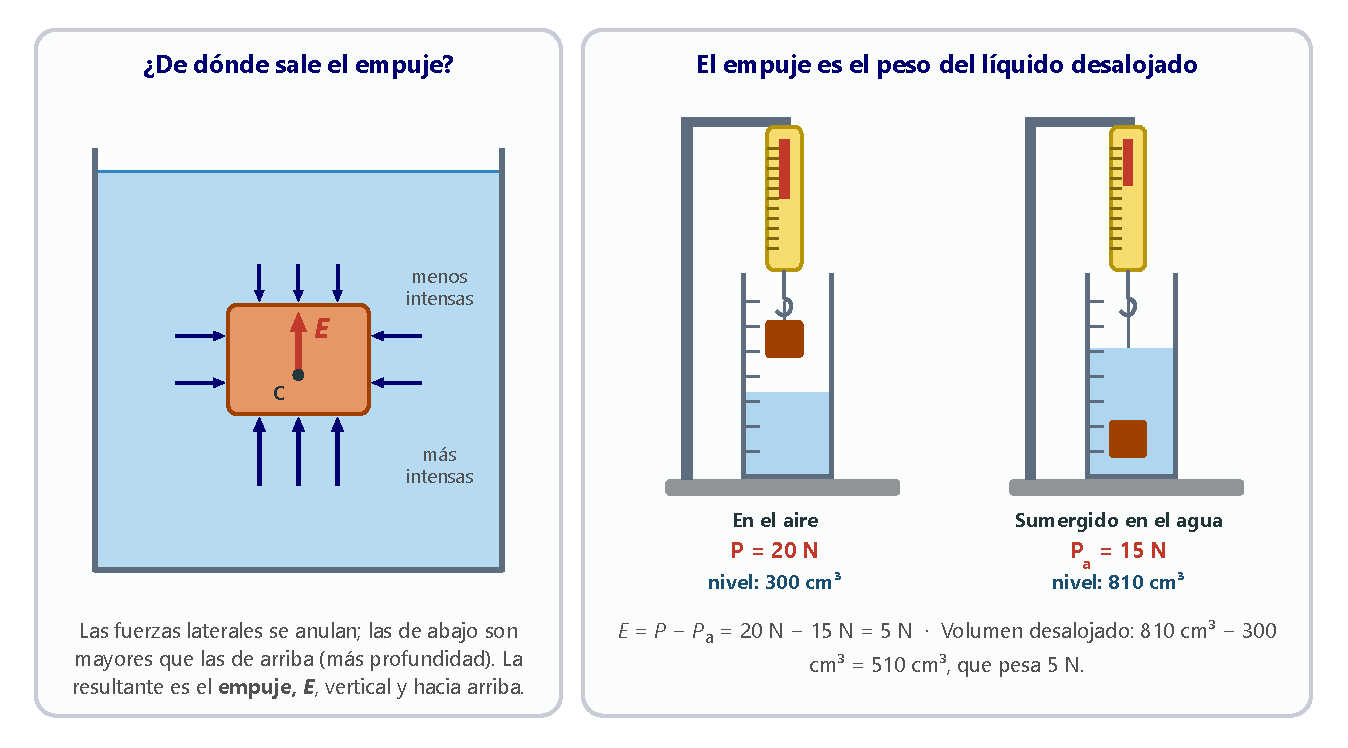
\includegraphics[width=\textwidth]{images/UD10/empuje}
    \caption{Origen de la fuerza de empuje y comprobación del principio de Arquímedes con un dinamómetro.}
    \label{fig:empuje}
\end{figure}

\subsection{¿Cómo se calcula el empuje? El peso aparente}

El empuje es el peso del fluido desalojado: \(E = m_{\text{fluido}} \cdot g\). Como \(m_{\text{fluido}} = \rho_{\text{fluido}} \cdot V_{\text{desalojado}}\), y el volumen desalojado es el volumen de la parte sumergida del cuerpo:
\[ E = V_{\text{sumergido}} \cdot \rho_{\text{fluido}} \cdot g \]

Se llama \textbf{peso aparente}, \(P_a\), al que marca el dinamómetro cuando el cuerpo está sumergido. Es el peso real menos el empuje:
\[ P_a = P - E \qquad\Rightarrow\qquad E = P - P_a \]
Si el cuerpo, de volumen \(V\), está totalmente sumergido, su peso es \(P = V \cdot \rho_{\text{cuerpo}} \cdot g\), y el peso aparente queda:
\[ P_a = V \cdot g \cdot (\rho_{\text{cuerpo}} - \rho_{\text{fluido}}) \]

El principio de Arquímedes es válido para todos los fluidos, líquidos y gases, y para cuerpos sumergidos total o parcialmente.

\begin{example}
    Una pieza de una aleación pesa \qty{400}{\newton} y ocupa \qty{5}{\cubic\dm}. Calcula el empuje que recibe al sumergirla en un líquido de densidad \qty{837}{\kg\per\cubic\m} y su peso aparente en él.
    \[ E = V \cdot \rho_{\text{líquido}} \cdot g = \num{5e-3} \cdot 837 \cdot \num{9.8} = \textcolor{red}{\qty{41}{\newton}} \qquad P_a = P - E = 400 - 41 = \textcolor{red}{\qty{359}{\newton}} \]
\end{example}

\subsection{¿Cómo se puede medir la densidad con el principio de Arquímedes?}

Muchos métodos para medir densidades se basan en este principio. Para un \textbf{sólido irregular}, basta con medir su peso en el aire, \(P\), y sumergido en agua, \(P_a\):
\begin{itemize}
    \item El empuje, \(E = P - P_a\), permite calcular el volumen: \(V = \dfrac{E}{\rho_{\text{agua}} \cdot g}\).
    \item El peso da la masa, \(m = P/g\), y la densidad es \(\rho = m/V\).
\end{itemize}
Combinando las dos expresiones se obtiene una fórmula muy cómoda: \(\rho_{\text{cuerpo}} = \rho_{\text{líquido}} \cdot \dfrac{P}{E}\).

Del mismo modo, si conocemos la densidad de un cuerpo, podemos medir la de un \textbf{líquido} pesando el cuerpo en el aire y sumergido en él. Los \textbf{densímetros} son tubos de vidrio lastrados que flotan en el líquido: cuanto más denso es, menos se hunden, y la densidad se lee en la escala, en la marca que coincide con la superficie.

\begin{example}
    Un objeto pesa \qty{300}{\newton} en el aire y \qty{200}{\newton} sumergido totalmente en agua. Calcula su volumen y su densidad.

    \(E = P - P_a = 300 - 200 = \qty{100}{\newton}\); \quad \(V = \dfrac{E}{\rho_{\text{agua}} \cdot g} = \dfrac{100}{1000 \cdot \num{9.8}} = \textcolor{red}{\qty{0.0102}{\cubic\m}}\).

    \(m = \dfrac{P}{g} = \dfrac{300}{\num{9.8}} = \qty{30.6}{\kg}\); \quad \(\rho = \dfrac{m}{V} = \dfrac{\num{30.6}}{\num{0.0102}} = \textcolor{red}{\qty{3000}{\kg\per\cubic\m}}\).

    Con la fórmula directa: \(\rho = 1000 \cdot \dfrac{300}{100} = \qty{3000}{\kg\per\cubic\m}\).
\end{example}

\begin{example}
    Una pieza de aluminio (\(\rho = \qty{2700}{\kg\per\cubic\m}\)) pesa \qty{350}{\newton} en el aire y \qty{230}{\newton} sumergida en un líquido. Calcula la densidad del líquido.

    \(E = 350 - 230 = \qty{120}{\newton}\). El volumen de la pieza es \(V = \dfrac{P}{\rho_{\text{Al}} \cdot g} = \dfrac{350}{2700 \cdot \num{9.8}} = \qty{0.01323}{\cubic\m}\), y por tanto:
    \[ \rho_{\text{líquido}} = \frac{E}{V \cdot g} = \frac{120}{\num{0.01323} \cdot \num{9.8}} = \textcolor{red}{\qty{926}{\kg\per\cubic\m}} \]
\end{example}

\subsection{¿Por qué flotan los cuerpos?}

Un cuerpo sumergido en un fluido está sometido a dos fuerzas: su \textbf{peso}, aplicado en su centro de gravedad, G, vertical y hacia abajo, y el \textbf{empuje}, aplicado en el centro de empuje, C, vertical y hacia arriba. Al soltarlo dentro del fluido puede ocurrir (figura~\ref{fig:flotacion}):
\begin{itemize}
    \item \(P > E\): el cuerpo \textbf{se hunde} hasta el fondo. Ocurre si \(\rho_{\text{cuerpo}} > \rho_{\text{fluido}}\); por ejemplo, una bola de hierro en agua.
    \item \(P = E\): el cuerpo queda \textbf{en equilibrio} dentro del fluido, sin subir ni bajar. Ocurre si \(\rho_{\text{cuerpo}} = \rho_{\text{fluido}}\); por ejemplo, un globo lleno de agua.
    \item \(P < E\): el cuerpo \textbf{sube y flota}. Ocurre si \(\rho_{\text{cuerpo}} < \rho_{\text{fluido}}\); por ejemplo, un corcho en agua. Al salir parcialmente, el volumen sumergido disminuye hasta que el empuje se iguala con el peso.
\end{itemize}

\begin{figure}[H]
    \centering
    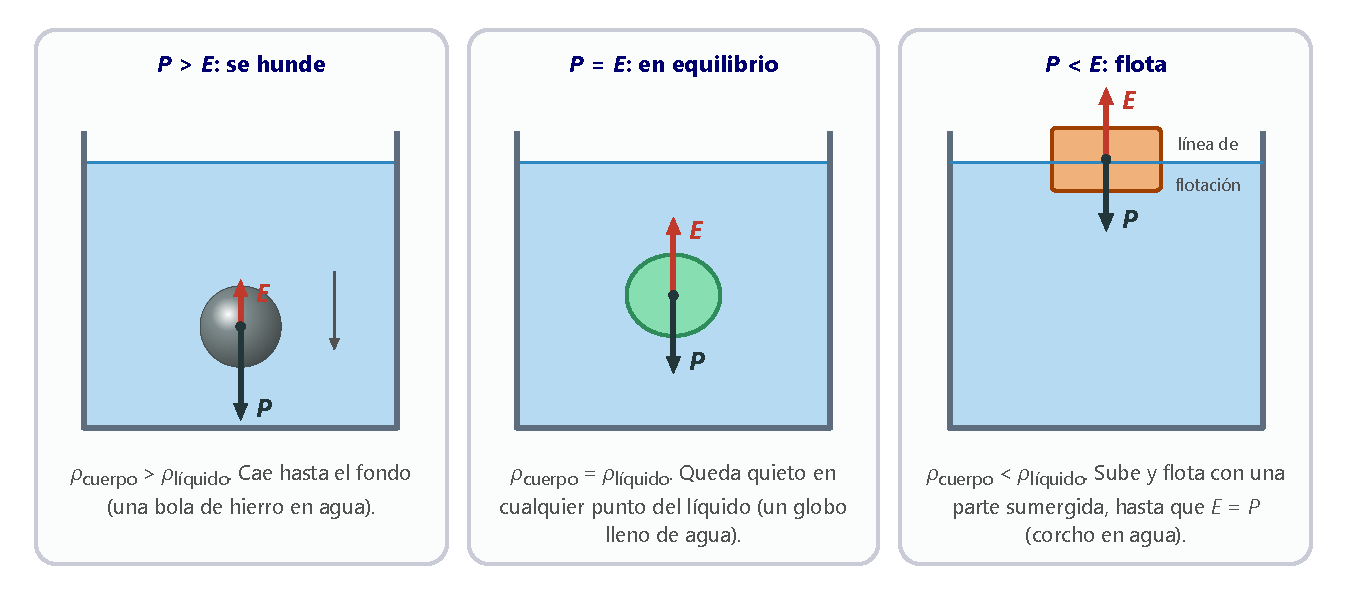
\includegraphics[width=\textwidth]{images/UD10/flotacion}
    \caption{Un cuerpo se hunde, queda en equilibrio o flota según sean su peso y el empuje.}
    \label{fig:flotacion}
\end{figure}

Para un cuerpo que flota, \(E = P\), es decir, \(V_{\text{sumergido}} \cdot \rho_{\text{fluido}} \cdot g = V \cdot \rho_{\text{cuerpo}} \cdot g\), de donde:
\[ \frac{V_{\text{sumergido}}}{V} = \frac{\rho_{\text{cuerpo}}}{\rho_{\text{fluido}}} \]

\begin{example}
    ¿Qué fracción de un iceberg queda bajo el agua? (\(\rho_{\text{hielo}} = \qty{917}{\kg\per\cubic\m}\); \(\rho_{\text{agua de mar}} = \qty{1030}{\kg\per\cubic\m}\)).
    \[ \frac{V_{\text{sumergido}}}{V} = \frac{917}{1030} = \num{0.89} \]
    El \textcolor{red}{\qty{89}{\percent}} del iceberg está sumergido: solo vemos la «punta del iceberg».
\end{example}

\paragraph{¿Por qué flota un barco de acero?} El acero es casi ocho veces más denso que el agua, pero un barco es hueco: su volumen total es enorme y su densidad \emph{media} (acero, aire y carga) es menor que la del agua. Al hundirse un poco desaloja mucha agua, y el empuje compensa su peso. La línea que separa la parte sumergida del casco de la que no lo está es la \textbf{línea de flotación}; si aumenta la carga, el barco se hunde más hasta que el empuje vuelve a igualar al peso.

Para que un barco esté en equilibrio estable, además de ser \(P = E\), el centro de gravedad y el centro de empuje deben estar en la misma vertical, y \textbf{G debe estar más bajo que C} (figura~\ref{fig:barco_globo}). Así, si una ola lo inclina, el par de fuerzas formado por el peso y el empuje lo vuelve a poner derecho. Por eso la carga pesada se coloca lo más abajo posible.

\paragraph{¿Por qué sube un globo aerostático?} El principio de Arquímedes también se cumple en el aire. Un globo se llena de aire caliente (o de helio), menos denso que el aire que lo rodea; como su volumen es muy grande, el empuje del aire es mayor que el peso total del globo, y sube.

\begin{figure}[H]
    \centering
    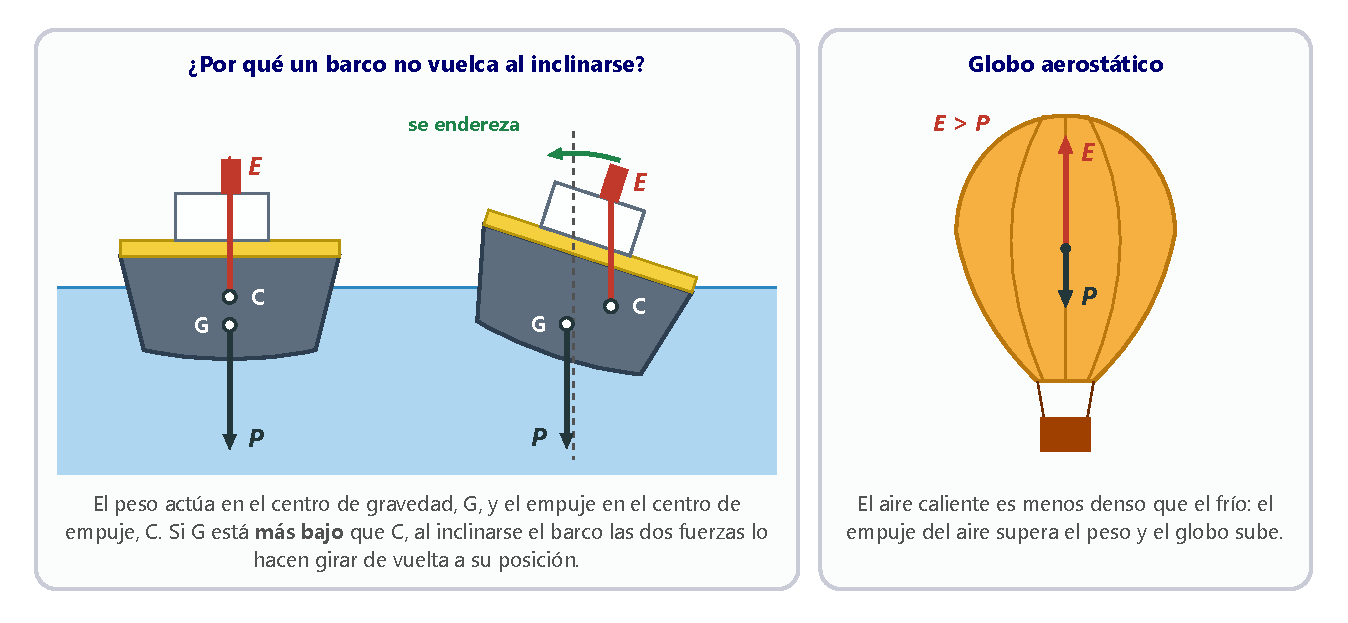
\includegraphics[width=\textwidth]{images/UD10/barco_globo}
    \caption{Estabilidad de un barco y flotación de un globo aerostático.}
    \label{fig:barco_globo}
\end{figure}

\begin{exercise}
    Una piedra pesa \qty{300}{\newton} en el aire y \qty{280}{\newton} sumergida en agua. ¿Cuál es su volumen?
    \begin{solu}
        \(E = P - P_a = 300 - 280 = \qty{20}{\newton}\); \(V = \dfrac{E}{\rho_{\text{agua}} \cdot g} = \dfrac{20}{1000 \cdot \num{9.8}} = \textcolor{red}{\qty{2.04e-3}{\cubic\m}} = \qty{2.04}{\cubic\dm}\).
    \end{solu}
\end{exercise}

\begin{exercise}
    Se sumerge en agua un cuerpo de \qty{300}{\gram} y \qty{20}{\cubic\cm}. ¿Cuál es su peso? ¿Qué empuje recibe? ¿Cuál es su peso aparente?
    \begin{solu}
        \(P = \num{0.300} \cdot \num{9.8} = \textcolor{red}{\qty{2.94}{\newton}}\); \quad \(E = \num{2e-5} \cdot 1000 \cdot \num{9.8} = \textcolor{red}{\qty{0.196}{\newton}}\); \quad \(P_a = \num{2.94} - \num{0.196} = \textcolor{red}{\qty{2.74}{\newton}}\).
    \end{solu}
\end{exercise}

\begin{exercise}
    Busca información sobre cómo se usa en el laboratorio un densímetro para medir la densidad de un líquido. ¿Por qué se hunde más en el alcohol que en el agua?
    \begin{solu}
        Respuesta libre. Se introduce el densímetro en una probeta con el líquido, se deja que flote libremente y se lee la marca de la escala que coincide con la superficie del líquido. En el alcohol, que es \textcolor{red}{menos denso}, el densímetro tiene que \textcolor{red}{desalojar más volumen} para que el empuje iguale a su peso, y por eso se hunde más.
    \end{solu}
\end{exercise}

\begin{exercise}
    Una esfera pesa \qty{176}{\newton} en el aire y \qty{126}{\newton} sumergida totalmente en agua. Calcula su volumen y su densidad.
    \begin{solu}
        \(E = 176 - 126 = \qty{50}{\newton}\); \(V = \dfrac{50}{1000 \cdot \num{9.8}} = \textcolor{red}{\qty{5.1e-3}{\cubic\m}}\).
        \(\rho = \rho_{\text{agua}} \cdot \dfrac{P}{E} = 1000 \cdot \dfrac{176}{50} = \textcolor{red}{\qty{3520}{\kg\per\cubic\m}}\).
    \end{solu}
\end{exercise}

\begin{exercise}
    Una pieza de plata (\(\rho = \qty{10500}{\kg\per\cubic\m}\)) pesa \qty{500}{\newton} en el aire y \qty{420}{\newton} sumergida en un líquido. Calcula la densidad del líquido.
    \begin{solu}
        \(E = 500 - 420 = \qty{80}{\newton}\); \(V = \dfrac{P}{\rho_{\text{plata}} \cdot g} = \dfrac{500}{10500 \cdot \num{9.8}} = \qty{4.86e-3}{\cubic\m}\).
        \(\rho_{\text{líquido}} = \dfrac{E}{V \cdot g} = \dfrac{80}{\num{4.86e-3} \cdot \num{9.8}} = \textcolor{red}{\qty{1680}{\kg\per\cubic\m}}\).
    \end{solu}
\end{exercise}

\begin{exercise}
    ¿Qué hace un submarino para sumergirse y para volver a la superficie?
    \begin{solu}
        Cambia su \textcolor{red}{peso} sin cambiar su volumen (y, por tanto, su empuje): para sumergirse \textcolor{red}{llena de agua} unos depósitos (tanques de lastre) y para subir los \textcolor{red}{vacía} expulsando el agua con aire comprimido.
    \end{solu}
\end{exercise}

\begin{exercise}
    ¿Cómo cambia la línea de flotación de un barco cuando pasa de un río al mar? ¿Por qué?
    \begin{solu}
        El agua del mar es \textcolor{red}{más densa} que la del río. Para conseguir el mismo empuje (igual al peso del barco) necesita desalojar menos volumen, así que en el mar el barco \textcolor{red}{se hunde menos}: la línea de flotación queda más alta respecto al agua.
    \end{solu}
\end{exercise}

\subsection*{Actividades de consolidación: empuje y principio de Arquímedes}

\begin{exercise}
    Justifica si son verdaderas o falsas estas afirmaciones:
    \begin{enumerate}[label=\alph*)]
        \item La línea de acción del empuje pasa siempre por el centro de gravedad del cuerpo sumergido.
        \item Dos cuerpos distintos del mismo volumen, totalmente sumergidos en el mismo líquido, reciben el mismo empuje.
        \item El empuje es igual a la diferencia entre el peso del cuerpo en el aire y su peso aparente en el líquido.
        \item El empuje es proporcional al volumen de líquido desalojado, a la gravedad y a la densidad del líquido.
    \end{enumerate}
    \begin{solu}
        a) \textcolor{red}{Falso}: pasa por el \emph{centro de empuje}, que es el centro de gravedad del fluido desalojado. Solo coincide con el centro de gravedad del cuerpo si este es homogéneo y está totalmente sumergido (en un barco, por ejemplo, no coinciden).
        b) \textcolor{red}{Verdadero}: el empuje depende del volumen desalojado, no del material. c) \textcolor{red}{Verdadero}. d) \textcolor{red}{Verdadero}: \(E = V \cdot \rho \cdot g\).
    \end{solu}
\end{exercise}

\begin{exercise}
    Explica qué ocurre en cada caso y qué conclusión general se obtiene:
    \begin{enumerate}[label=\Alph*)]
        \item Un globo de aire caliente en el aire frío.
        \item Un bloque de densidad \qty{300}{\kg\per\cubic\m} en agua.
        \item Un bloque de densidad \qty{790}{\kg\per\cubic\m} en agua.
        \item Un bloque de densidad \qty{790}{\kg\per\cubic\m} en alcohol (\qty{790}{\kg\per\cubic\m}).
        \item Un bloque de plomo (\qty{11300}{\kg\per\cubic\m}) en agua.
    \end{enumerate}
    \begin{solu}
        A) El aire caliente es menos denso que el frío: el globo \textcolor{red}{sube}.
        B) Flota con solo el \qty{30}{\percent} de su volumen sumergido.
        C) También \textcolor{red}{flota}, pero más hundido que B: el \qty{79}{\percent} de su volumen está sumergido.
        D) Las densidades son iguales: queda \textcolor{red}{en equilibrio} en cualquier punto del líquido.
        E) Es mucho más denso que el agua: \textcolor{red}{se hunde}.
        Conclusión: un cuerpo \textcolor{red}{flota} si es menos denso que el fluido, queda \textcolor{red}{en equilibrio} si tiene su misma densidad y \textcolor{red}{se hunde} si es más denso.
    \end{solu}
\end{exercise}

\begin{exercise}
    Queremos saber si una joya es de oro puro (\(\rho = \qty{19300}{\kg\per\cubic\m}\)). Su masa es de \qty{0.120}{\kg} y, sumergida en agua, su peso aparente equivale al de una masa \qty{8}{\gram} menor. ¿Es de oro puro?
    \begin{solu}
        El empuje equivale al peso de \qty{8}{\gram} de agua, que ocupan \qty{8}{\cubic\cm}: \(V_{\text{joya}} = \qty{8e-6}{\cubic\m}\).
        \(\rho = \dfrac{\num{0.120}}{\num{8e-6}} = \qty{15000}{\kg\per\cubic\m}\). Es menor que la del oro: \textcolor{red}{no es de oro puro}.
    \end{solu}
\end{exercise}

\begin{exercise}
    Un objeto de \qty{10000}{\newton} de peso ocupa \qty{10}{\cubic\m}. ¿Flotará en un tanque lleno de aceite de densidad \qty{935}{\kg\per\cubic\m}? ¿Qué fracción de su volumen quedará sumergida?
    \begin{solu}
        \(m = \dfrac{10000}{\num{9.8}} = \qty{1020}{\kg}\); \(\rho = \dfrac{1020}{10} = \qty{102}{\kg\per\cubic\m}\). Es menos denso que el aceite: \textcolor{red}{sí flota}.
        Fracción sumergida: \(\dfrac{102}{935} = \num{0.11}\), es decir, el \textcolor{red}{\qty{11}{\percent}}.
    \end{solu}
\end{exercise}

\begin{exercise}
    Un cubo de madera de \qty{10}{\cm} de arista flota en agua con \qty{6}{\cm} sumergidos. ¿Cuál es la densidad de la madera? ¿Cuántos centímetros se hundiría en aceite de densidad \qty{800}{\kg\per\cubic\m}?
    \begin{solu}
        \(\dfrac{\rho_{\text{madera}}}{\rho_{\text{agua}}} = \dfrac{V_{\text{sumergido}}}{V} = \dfrac{6}{10} \Rightarrow \rho_{\text{madera}} = \textcolor{red}{\qty{600}{\kg\per\cubic\m}}\).
        En aceite: \(\dfrac{h}{10} = \dfrac{600}{800} = \num{0.75} \Rightarrow h = \textcolor{red}{\qty{7.5}{\cm}}\).
    \end{solu}
\end{exercise}


%------------------------------------------------


    \chapterimage{images/portada_cabeceras/cabecera_UD11}
    \chapter{Trabajo y energía mecánica}

    %! Author = crist
%! Date = 25/10/2026

\spacing{1.3}
%----------------------------------------------------------------------------------------
%	UNIDAD 11: TRABAJO Y ENERGÍA MECÁNICA (4.º ESO)
%   Figuras: images/UD11/*.pdf (fuente HTML en images/UD11/html, SVG en images/UD11/svg)
%   Gráficas con pgfplots: estilo «grafica», definido al inicio de la UD7.
%   Datos usados en toda la unidad: g = 9,8 m/s²; 1 kW·h = 3,6·10^6 J; 1 eV = 1,6·10^-19 J; 1 CV = 736 W.
%----------------------------------------------------------------------------------------
\DeclareSIUnit\CV{CV}

% Mapa conceptual del tema (fuente en images/mapas_conceptuales/html/temas.js)
\begin{figure}[H]
    \centering
    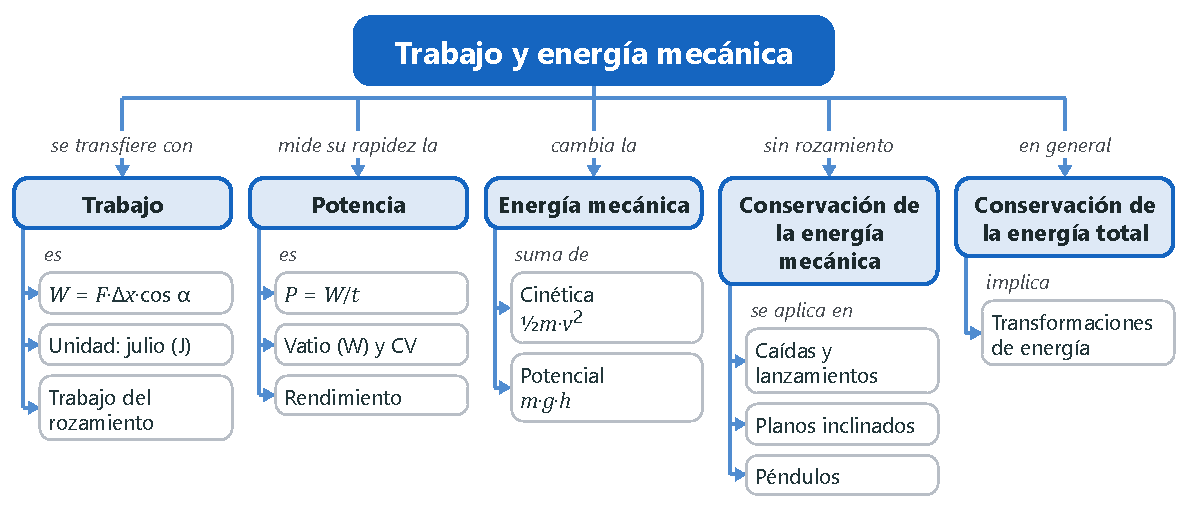
\includegraphics[width=\textwidth]{images/mapas_conceptuales/mapa_UD11}
\end{figure}

%========================================================================================
%\section*{Para empezar: el consumo de electricidad y de gas}
%\addcontentsline{toc}{section}{Para empezar: el consumo de electricidad y de gas}
%========================================================================================
%
%La electricidad nos proporciona energía para realizar trabajo: la usan todos los electrodomésticos y todos los aparatos con motores eléctricos. Las compañías venden la electricidad por «unidades», y esa unidad es el \textbf{kilovatio hora} (\unit{\kilo\watt\hour}). El contador de casa registra los kilovatios hora consumidos, y el precio depende del contrato con la comercializadora. Un electrodoméstico de gran potencia consume energía más deprisa, por lo que su funcionamiento resulta más caro que el de uno de menor potencia.
%
%Con el gas natural ocurre algo parecido. El contador mide el volumen de gas en metros cúbicos, pero en la factura el consumo aparece en kilovatios hora: no se paga por el volumen, sino por la \textbf{energía} que proporciona el gas al quemarse. Como el volumen de un gas cambia con la presión y la temperatura, y no todos los gases tienen la misma composición, cada compañía aplica un «factor de conversión»: cada metro cúbico de gas natural aporta unos \qty{11}{\kilo\watt\hour}. En el caso del gas butano, que se vende en bombonas de \qty{12.5}{\kg}, cada bombona proporciona unos \qty{159}{\kilo\watt\hour}.
%
%Consumir energía de forma eficiente y elegir fuentes renovables tiene que ver con el \textbf{ODS 7} (\emph{Energía asequible y no contaminante}), que busca aumentar el uso de energías renovables y mejorar la eficiencia energética, y con el \textbf{ODS 12} (\emph{Producción y consumo responsables}), que pide un uso eficiente de los recursos naturales.
%
%En esta unidad estudiaremos qué es el \textbf{trabajo} para la física, cómo se mide la rapidez con que se realiza (la \textbf{potencia}) y qué es la \textbf{energía mecánica}, y descubriremos una de las leyes más importantes de la naturaleza: la conservación de la energía.
%
%\begin{exercise}
%    Haz una lista de aparatos que usen electricidad, en casa y en el instituto. Anota la potencia de algunos de ellos (viene en la etiqueta), estima cuántas horas funcionan al día y calcula la energía diaria que consumen en \unit{\kilo\watt\hour}.
%    \begin{solu}
%        Respuesta libre. Ejemplos: iluminación, ordenador, frigorífico, lavadora, horno, microondas, calefacción\ldots{} La energía se calcula como \(E = P \cdot t\): por ejemplo, un microondas de \qty{800}{\watt} que funciona \qty{15}{\minute} al día consume \(\num{0.8} \cdot \num{0.25} = \textcolor{red}{\qty{0.2}{\kilo\watt\hour}}\) diarios; una lavadora consume entre \qty{0.5}{\kilo\watt\hour} y \qty{1.5}{\kilo\watt\hour} por lavado, según la temperatura del agua.
%    \end{solu}
%\end{exercise}
%
%\begin{exercise}
%    ¿Por qué cuesta más hacer funcionar un electrodoméstico de mayor potencia que otro del mismo tipo con menos potencia?
%    \begin{solu}
%        Porque un aparato de mayor potencia \textcolor{red}{consume más energía en el mismo tiempo}, y lo que se paga es la energía consumida (los \unit{\kilo\watt\hour}).
%    \end{solu}
%\end{exercise}
%
%\begin{exercise}
%    Si el contador mide el gas en \unit{\cubic\m}, ¿por qué en la factura se indica en \unit{\kilo\watt\hour}? ¿Aportan la misma energía todos los metros cúbicos de gas?
%    \begin{solu}
%        Porque el gas \textcolor{red}{no se paga por su volumen, sino por la energía que proporciona}. Un metro cúbico de gas no siempre aporta la misma energía: depende de la presión, de la temperatura y de la composición del gas, por eso la compañía aplica un factor de conversión.
%    \end{solu}
%\end{exercise}
%
%\begin{exercise}
%    Una bombona de butano de \qty{12.5}{\kg} proporciona unos \qty{159}{\kilo\watt\hour}. ¿Cuánta energía aporta cada kilogramo de butano, en \unit{\kilo\watt\hour} y en julios?
%    \begin{solu}
%        \(\dfrac{159}{\num{12.5}} = \textcolor{red}{\qty{12.7}{\kilo\watt\hour}}\) por kilogramo, es decir, \(\num{12.7} \cdot \num{3.6e6} = \textcolor{red}{\qty{4.6e7}{\joule}}\).
%    \end{solu}
%\end{exercise}

%========================================================================================
\section{Trabajo y energía}
%========================================================================================

¿Estás haciendo trabajo mientras esperas el autobús con la mochila a la espalda? Si respondes que sí, estás confundiendo el esfuerzo muscular con el trabajo. Al sostener la mochila sin moverte te cansas, pero para la física no realizas ningún trabajo, porque no hay desplazamiento.

\begin{definition}[Trabajo]
    En física, decimos que una fuerza realiza un \textbf{trabajo} cuando produce un \textbf{desplazamiento} en la dirección de la fuerza.
\end{definition}

Un coche que se ha quedado sin gasolina en lo alto de una cuesta parece que no tiene energía. Sin embargo, si se suelta el freno, rodará cuesta abajo: tiene energía por estar a cierta altura.

\begin{definition}[Energía]
    La \textbf{energía} es la capacidad que tienen los cuerpos de producir transformaciones, por ejemplo, de realizar un trabajo.
\end{definition}

El trabajo y la energía son \textbf{magnitudes escalares}: quedan definidas con un número y su unidad, que en el SI es el \textbf{julio} (\unit{\joule}). De hecho, el trabajo es una forma de medir la energía que se transfiere de un cuerpo a otro.

\subsection{¿Cuándo realiza trabajo una fuerza?}

\begin{itemize}
    \item \textbf{Sin desplazamiento no hay trabajo.} Al empujar una pared, los músculos ejercen una fuerza, pero la pared no se mueve: no se realiza trabajo.
    \item \textbf{El desplazamiento debe producirse en la dirección de la fuerza.} Si llevamos una caja en brazos por un pasillo horizontal, la fuerza que hacemos para sostenerla es vertical y el desplazamiento es horizontal: esa fuerza no realiza trabajo.
\end{itemize}

\begin{figure}[H]
    \centering
    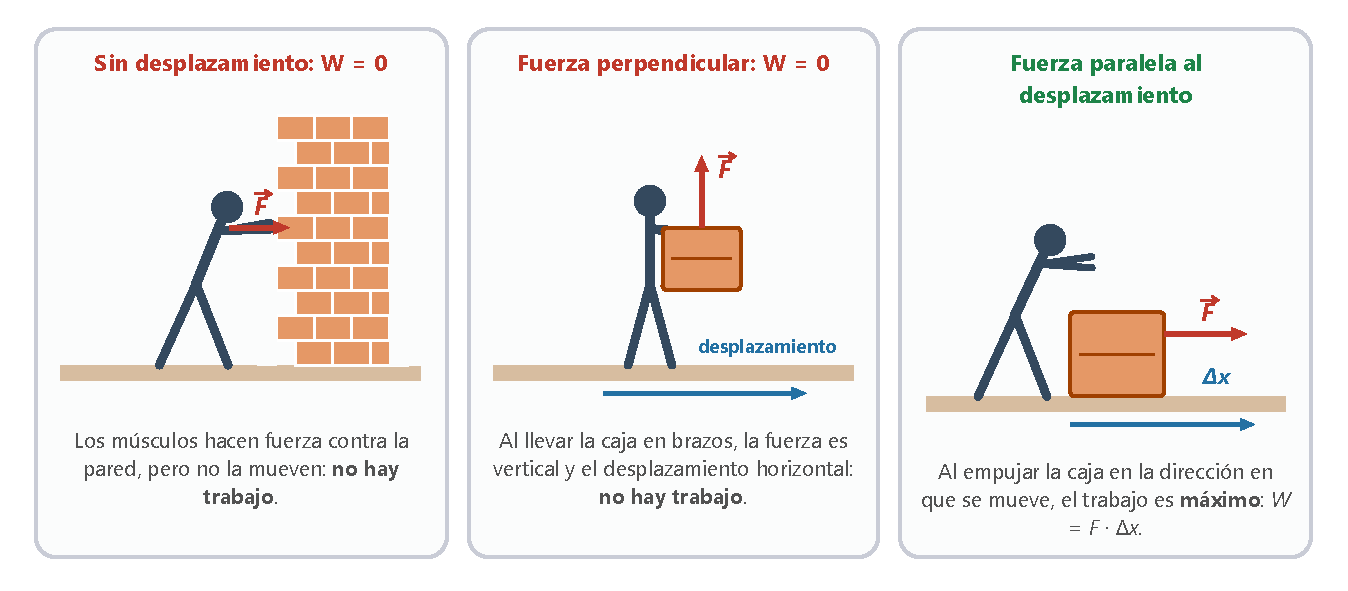
\includegraphics[width=\textwidth]{images/UD11/trabajo_casos}
    \caption{Solo hay trabajo si la fuerza produce un desplazamiento en su dirección.}
    \label{fig:trabajo_casos}
\end{figure}

\begin{exercise}
    ¿Realizas trabajo al levantar la mochila desde el suelo hasta la altura a la que la sostienes? ¿Y al subir una escalera con la mochila a cuestas?
    \begin{solu}
        \textcolor{red}{Sí en los dos casos}: ejerces una fuerza vertical, hacia arriba, para vencer el peso de la mochila, y la mochila se desplaza en esa misma dirección (sube).
    \end{solu}
\end{exercise}

\begin{exercise}
    Responde verdadero o falso y justifica tu respuesta:
    \begin{enumerate}[label=\alph*)]
        \item Siempre que hacemos un esfuerzo muscular se realiza trabajo.
        \item Nuestros brazos realizan trabajo al llevar la bolsa de la compra desde el supermercado hasta casa por una calle horizontal.
        \item La energía es la capacidad que tienen los cuerpos de realizar un trabajo.
        \item Realizamos un trabajo cuando empujamos fuertemente una pared.
    \end{enumerate}
    \begin{solu}
        a) \textcolor{red}{Falso}: si no hay desplazamiento, no hay trabajo. b) \textcolor{red}{Falso}: la fuerza de los brazos es vertical y el desplazamiento horizontal. c) \textcolor{red}{Verdadero}. d) \textcolor{red}{Falso}: la pared no se desplaza.
    \end{solu}
\end{exercise}

\subsection*{Actividades de consolidación: trabajo y energía}

\begin{exercise}
    ¿Coincide el significado de la palabra \emph{trabajo} en el lenguaje cotidiano y en física?
    \begin{solu}
        \textcolor{red}{No}. En el lenguaje cotidiano el trabajo se relaciona con el esfuerzo o el cansancio, haya o no desplazamiento; en física solo hay trabajo si una \textcolor{red}{fuerza produce un desplazamiento} en su dirección.
    \end{solu}
\end{exercise}

\begin{exercise}
    ¿Realizas trabajo, en el sentido físico, mientras resuelves estas cuestiones en clase?
    \begin{solu}
        Prácticamente \textcolor{red}{no}: aunque pensar cansa, no ejerces ninguna fuerza que desplace un cuerpo (salvo el pequeño trabajo de mover el bolígrafo).
    \end{solu}
\end{exercise}

\begin{exercise}
    Explica si realizas trabajo o no cuando:
    \begin{enumerate}[label=\alph*)]
        \item Levantas una maleta desde el suelo.
        \item Esperas el tren en el andén con la maleta en la mano.
        \item Subes las escaleras con la maleta.
        \item Empujas con fuerza la pared de tu habitación.
    \end{enumerate}
    \begin{solu}
        a) \textcolor{red}{Sí}: la fuerza y el desplazamiento son verticales. b) \textcolor{red}{No}: no hay desplazamiento. c) \textcolor{red}{Sí}: la maleta sube en la dirección de la fuerza. d) \textcolor{red}{No}: la pared no se desplaza.
    \end{solu}
\end{exercise}

\begin{exercise}
    Indica en cuáles de estas situaciones se realiza trabajo y en cuáles no: a) una persona empuja un mueble y lo desplaza por el suelo; b) un alumno camina por un pasillo con la mochila a la espalda; c) una persona levanta del suelo una bolsa de la compra; d) una persona está quieta sosteniendo una bolsa.
    \begin{solu}
        Se realiza trabajo en \textcolor{red}{a) y c)}. En b) la fuerza que sostiene la mochila es perpendicular al desplazamiento, y en d) no hay desplazamiento.
    \end{solu}
\end{exercise}

%========================================================================================
\section{Trabajo realizado por una fuerza constante}
%========================================================================================

Cuando una fuerza constante tiene la misma dirección y sentido que el desplazamiento que produce, el trabajo es el producto de la fuerza por el desplazamiento:
\[ \text{trabajo} = \text{fuerza} \times \text{desplazamiento} \qquad W = F \cdot \Delta x \]
donde \(W\) es el trabajo, \(F\) es la fuerza (constante) y \(\Delta x\) el desplazamiento producido en la dirección de la fuerza.

En una gráfica fuerza-desplazamiento, una fuerza constante es una recta horizontal, y el trabajo que realiza es el \textbf{área del rectángulo} que queda bajo ella: base (\(\Delta x\)) por altura (\(F\)).

\begin{center}
    \begin{tikzpicture}
        \begin{axis}[grafica, width=8cm, height=5cm, xlabel={\(x\) (m)}, ylabel={\(F\) (N)}, xmin=0, xmax=4.5, ymin=0, ymax=7.5, title={\small \(W = F \cdot \Delta x = 6 \cdot \num{2.5} = \qty{15}{\joule}\) (área del rectángulo)}]
            \addplot[mark=none, fill=yellow!60, draw=red!75!black, line width=1.4pt] coordinates {(0,0) (0,6) (2.5,6) (2.5,0)};
            \node at (axis cs:1.25,3) {\(W\)};
        \end{axis}
    \end{tikzpicture}
\end{center}

\subsection{¿En qué unidad se expresa el trabajo?}

En el SI, el trabajo se mide en \textbf{julios} (\unit{\joule}). Un julio es el trabajo que realiza una fuerza de un newton al desplazar su punto de aplicación un metro en su misma dirección:
\[ \qty{1}{\joule} = \qty{1}{\newton} \cdot \qty{1}{\m} \]
Su ecuación de dimensiones es \([W] = \mathrm{M \cdot L^2 \cdot T^{-2}}\).

\subsection{¿Qué sucede si la fuerza tiene la dirección y el sentido del desplazamiento?}

Entonces el trabajo es \textbf{máximo y positivo}: \(W = F \cdot \Delta x\). Cuando empujamos un baúl en la misma dirección en la que queremos moverlo, aprovechamos toda la fuerza.

\begin{example}
    Calcula el trabajo que realizas al subir una mochila de \qty{8}{\kg} hasta una altura de \qty{1.5}{\m}.

    Para subirla hay que ejercer una fuerza igual a su peso: \(F = m \cdot g = 8 \cdot \num{9.8} = \qty{78.4}{\newton}\). Como la fuerza y el desplazamiento son verticales y hacia arriba:
    \[ W = F \cdot \Delta x = \num{78.4} \cdot \num{1.5} = \textcolor{red}{\qty{117.6}{\joule}} \]
\end{example}

\subsection{¿Qué sucede si la fuerza es perpendicular al desplazamiento?}

El trabajo realizado por esa fuerza es \textbf{nulo}: \(W = 0\). Si llevamos el baúl en brazos de un sitio a otro por un suelo horizontal, la fuerza que hacemos es vertical y el desplazamiento horizontal: no realizamos trabajo (figura~\ref{fig:trabajo_casos}).

\subsection{¿Realiza trabajo la fuerza de rozamiento?}

Sí, pero su trabajo es \textbf{negativo}, porque la fuerza de rozamiento tiene sentido contrario al desplazamiento (figura~\ref{fig:trabajo_angulo}):
\[ W_{\text{roz}} = -F_{\text{roz}} \cdot \Delta x \]
Recuerda que, en una superficie horizontal, \(F_{\text{roz}} = \mu \cdot m \cdot g\), donde \(\mu\) es el coeficiente de rozamiento.

\begin{example}
    Arrastras una mochila de \qty{10}{\kg} \qty{2}{\m} por un suelo horizontal. Si el coeficiente de rozamiento es \(\mu = \num{0.1}\), ¿qué trabajo realiza la fuerza de rozamiento?
    \[ W_{\text{roz}} = -\mu \cdot m \cdot g \cdot \Delta x = -\num{0.1} \cdot 10 \cdot \num{9.8} \cdot 2 = \textcolor{red}{\qty{-19.6}{\joule}} \]
\end{example}

\subsection{¿Y si la fuerza forma un ángulo con el desplazamiento?}

Cuando la fuerza forma un ángulo \(\theta\) con el desplazamiento, \textbf{solo realiza trabajo la componente de la fuerza en la dirección del desplazamiento}, \(F_x = F \cdot \cos\theta\) (figura~\ref{fig:trabajo_angulo}). Por tanto:
\[ W = F_x \cdot \Delta x = F \cdot \Delta x \cdot \cos\theta \]
Esta expresión incluye los casos anteriores: si \(\theta = \ang{0}\), \(\cos\theta = 1\) y el trabajo es máximo; si \(\theta = \ang{90}\), \(\cos\theta = 0\) y el trabajo es nulo; si \(\theta = \ang{180}\) (como el rozamiento), \(\cos\theta = -1\) y el trabajo es negativo.

\begin{figure}[H]
    \centering
    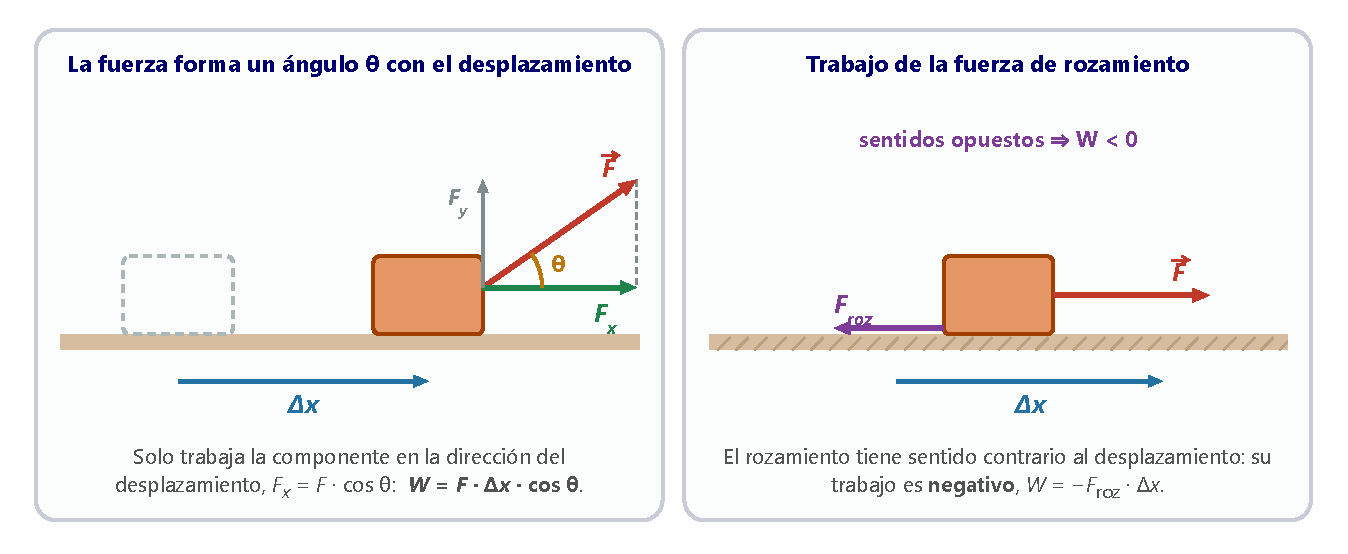
\includegraphics[width=\textwidth]{images/UD11/trabajo_angulo}
    \caption{Trabajo de una fuerza que forma un ángulo con el desplazamiento y de la fuerza de rozamiento.}
    \label{fig:trabajo_angulo}
\end{figure}

\begin{example}
    Arrastras una mochila \qty{2}{\m} por un suelo sin rozamiento tirando de ella con una fuerza de \qty{50}{\newton} que forma un ángulo de \ang{60} con la horizontal. ¿Qué trabajo realizas?
    \[ W = F \cdot \Delta x \cdot \cos\theta = 50 \cdot 2 \cdot \cos\ang{60} = 50 \cdot 2 \cdot \num{0.5} = \textcolor{red}{\qty{50}{\joule}} \]
    Solo se aprovecha la mitad de la fuerza: la componente vertical no realiza trabajo.
\end{example}

\begin{exercise}
    Escribe la ecuación de dimensiones del trabajo.
    \begin{solu}
        \([W] = [F] \cdot [\Delta x] = \mathrm{M \cdot L \cdot T^{-2}} \cdot \mathrm{L} = \textcolor{red}{\mathrm{M \cdot L^2 \cdot T^{-2}}}\).
    \end{solu}
\end{exercise}

\begin{exercise}
    En esta gráfica se representa una fuerza en función del desplazamiento que produce. ¿Cuánto vale la fuerza? ¿Qué desplazamiento produce? Calcula el trabajo que realiza.
    \begin{center}
        \begin{tikzpicture}
            \begin{axis}[grafica, width=6.5cm, height=4.2cm, xlabel={\(x\) (m)}, ylabel={\(F\) (N)}, xmin=0, xmax=5, ymin=0, ymax=10, ytick={0,2,...,10}]
                \addplot[mark=none, fill=yellow!60, draw=red!75!black, line width=1.4pt] coordinates {(0,0) (0,8) (4,8) (4,0)};
            \end{axis}
        \end{tikzpicture}
    \end{center}
    \begin{solu}
        La fuerza vale \textcolor{red}{\qty{8}{\newton}} y produce un desplazamiento de \textcolor{red}{\qty{4}{\m}}. El trabajo es el área del rectángulo: \(W = 8 \cdot 4 = \textcolor{red}{\qty{32}{\joule}}\).
    \end{solu}
\end{exercise}

\begin{exercise}
    ¿Puede ser nulo el trabajo de una fuerza aunque ni la fuerza ni el desplazamiento sean nulos?
    \begin{solu}
        \textcolor{red}{Sí}, cuando la fuerza es \textcolor{red}{perpendicular} al desplazamiento (\(\cos\ang{90} = 0\)).
    \end{solu}
\end{exercise}

\begin{exercise}
    Calcula el trabajo que realizas al arrastrar un baúl \qty{5}{\m} por un suelo horizontal sin rozamiento aplicando una fuerza de \qty{50}{\newton} que forma un ángulo de \ang{30} con la horizontal.
    \begin{solu}
        \(W = F \cdot \Delta x \cdot \cos\theta = 50 \cdot 5 \cdot \cos\ang{30} = 250 \cdot \num{0.866} = \textcolor{red}{\qty{216.5}{\joule}}\).
    \end{solu}
\end{exercise}

\begin{exercise}
    Una operaria arrastra un fardo \qty{10}{\m} por el suelo, sin rozamiento, con un cable que forma un ángulo de \ang{45} con la horizontal. Si el trabajo realizado es de \qty{1273}{\joule}, ¿qué fuerza ha aplicado?
    \begin{solu}
        \(F = \dfrac{W}{\Delta x \cdot \cos\theta} = \dfrac{1273}{10 \cdot \cos\ang{45}} = \dfrac{1273}{\num{7.07}} = \textcolor{red}{\qty{180}{\newton}}\).
    \end{solu}
\end{exercise}

\begin{exercise}
    Un reponedor arrastra un fardo de \qty{50}{\kg} una distancia de \qty{5}{\m} por una superficie horizontal sin rozamiento, tirando de un cable que forma \ang{30} con la horizontal. ¿Qué trabajo realiza si la fuerza que aplica es igual al peso del fardo?
    \begin{solu}
        \(F = 50 \cdot \num{9.8} = \qty{490}{\newton}\); \(W = 490 \cdot 5 \cdot \cos\ang{30} = \textcolor{red}{\qty{2122}{\joule}}\).
    \end{solu}
\end{exercise}

\subsection*{Actividades de consolidación: trabajo de una fuerza constante}

\begin{exercise}
    De la expresión del trabajo, \(W = F \cdot \Delta x\), se deduce también que \(F = W/\Delta x\) y \(\Delta x = W/F\). Úsalas para completar la tabla en tu cuaderno:
    \begin{center}
        % --- tabla antigua ---
        % \begin{tblr}{colspec={ccc}, hlines, vlines, row{1}={bg=ocre!85, fg=white, font=\bfseries}}
            % Fuerza (N) & Desplazamiento (m) & Trabajo (J) \\
            % 200 & \num{2.00} & \ldots \\
            % \ldots & \num{5.00} & 500 \\
            % 50 & \ldots & 100 \\
        % \end{tblr}
        % --- tabla nueva ---
        \begin{tabular}{@{}ccc@{}}
            \toprule
            \textbf{Fuerza (N)} & \textbf{Desplazamiento (m)} & \textbf{Trabajo (J)} \\
            \midrule
            200 & \num{2.00} & \ldots \\[3pt]
            \ldots & \num{5.00} & 500 \\[3pt]
            50 & \ldots & 100 \\
            \bottomrule
        \end{tabular}
    \end{center}
    \begin{solu}
        \(W = 200 \cdot 2 = \textcolor{red}{\qty{400}{\joule}}\); \(F = \dfrac{500}{5} = \textcolor{red}{\qty{100}{\newton}}\); \(\Delta x = \dfrac{100}{50} = \textcolor{red}{\qty{2}{\m}}\).
    \end{solu}
\end{exercise}

\begin{exercise}
    ¿Qué trabajo realizas al subir un paquete de \qty{4.5}{\kg} desde el suelo hasta una mesa de \qty{90}{\cm} de altura? ¿Y al llevarlo después en brazos por el pasillo de tu casa?
    \begin{solu}
        Subirlo: \(W = m \cdot g \cdot h = \num{4.5} \cdot \num{9.8} \cdot \num{0.9} = \textcolor{red}{\qty{39.7}{\joule}}\). Por el pasillo: \textcolor{red}{\qty{0}{\joule}}, porque la fuerza que hacemos (vertical) es perpendicular al desplazamiento (horizontal).
    \end{solu}
\end{exercise}

\begin{exercise}
    ¿Qué trabajo se realiza cuando una fuerza desplaza su punto de aplicación, en su misma dirección: a) \qty{3.0}{\m}, si la fuerza es de \qty{6}{\newton}; b) \qty{0.5}{\m}, si es de \qty{12}{\newton}; c) \qty{10}{\mm}, si es de \qty{10}{\newton}?
    \begin{solu}
        a) \(6 \cdot 3 = \textcolor{red}{\qty{18}{\joule}}\); b) \(12 \cdot \num{0.5} = \textcolor{red}{\qty{6}{\joule}}\); c) \(10 \cdot \num{0.010} = \textcolor{red}{\qty{0.1}{\joule}}\).
    \end{solu}
\end{exercise}

\begin{exercise}
    Una fuerza constante de \qty{9}{\newton} desplaza su punto de aplicación \qty{6}{\m} en su misma dirección. Dibuja la gráfica \(F\)--\(x\) y calcula el trabajo a partir de ella.
    \begin{solu}
        La gráfica es una recta horizontal a la altura \(F = \qty{9}{\newton}\) entre \(x = 0\) y \(x = \qty{6}{\m}\). El trabajo es el área del rectángulo: \(W = 9 \cdot 6 = \textcolor{red}{\qty{54}{\joule}}\).
    \end{solu}
\end{exercise}

\begin{exercise}
    Calcula el trabajo que realiza la fuerza de rozamiento cuando se arrastra una maleta de \qty{40}{\kg} \qty{5}{\m} sobre un suelo horizontal, si el coeficiente de rozamiento es \num{0.1}.
    \begin{solu}
        \(W_{\text{roz}} = -\mu \cdot m \cdot g \cdot \Delta x = -\num{0.1} \cdot 40 \cdot \num{9.8} \cdot 5 = \textcolor{red}{\qty{-196}{\joule}}\).
    \end{solu}
\end{exercise}

\begin{exercise}
    Arrastras un baúl de \qty{14}{\kg} \qty{4}{\m} por un suelo horizontal con un coeficiente de rozamiento de \num{0.1}. ¿Qué trabajo realiza la fuerza de rozamiento?
    \begin{solu}
        \(W_{\text{roz}} = -\num{0.1} \cdot 14 \cdot \num{9.8} \cdot 4 = \textcolor{red}{\qty{-54.9}{\joule}}\).
    \end{solu}
\end{exercise}

\begin{exercise}
    Una persona arrastra una caja de \qty{10}{\kg} \qty{10}{\m} por un suelo horizontal tirando con una fuerza constante de \qty{100}{\newton} que forma \ang{40} con la horizontal. La fuerza de rozamiento es de \qty{50}{\newton}. Calcula el trabajo realizado: a) por la fuerza de \qty{100}{\newton}; b) por el rozamiento; c) en total (trabajo neto).
    \begin{solu}
        a) \(W = 100 \cdot 10 \cdot \cos\ang{40} = \textcolor{red}{\qty{766}{\joule}}\). b) \(W_{\text{roz}} = -50 \cdot 10 = \textcolor{red}{\qty{-500}{\joule}}\). c) \(W_{\text{neto}} = 766 - 500 = \textcolor{red}{\qty{266}{\joule}}\). (El peso y la normal no realizan trabajo, porque son perpendiculares al desplazamiento.)
    \end{solu}
\end{exercise}

\begin{exercise}
    Una fuerza constante de \qty{25}{\newton} actúa sobre un cuerpo de \qty{10}{\kg} que se desplaza \qty{10}{\m} por un plano horizontal, en la dirección de la fuerza. Si el coeficiente de rozamiento es \num{0.1}, calcula el trabajo: a) de la fuerza aplicada; b) de la fuerza de rozamiento; c) total.
    \begin{solu}
        a) \(W = 25 \cdot 10 = \textcolor{red}{\qty{250}{\joule}}\). b) \(W_{\text{roz}} = -\num{0.1} \cdot 10 \cdot \num{9.8} \cdot 10 = \textcolor{red}{\qty{-98}{\joule}}\). c) \(W_{\text{total}} = 250 - 98 = \textcolor{red}{\qty{152}{\joule}}\).
    \end{solu}
\end{exercise}

%========================================================================================
\section[La potencia]{Relación trabajo-tiempo: la potencia}
%========================================================================================

Cuando subes unas escaleras corriendo, haces el mismo trabajo que cuando las subes despacio (elevas tu peso la misma altura), pero lo haces en menos tiempo: desarrollas más \textbf{potencia}.

\begin{definition}[Potencia]
    La \textbf{potencia}, \(P\), es la magnitud que mide la rapidez con la que se realiza un trabajo:
    \[ \text{potencia} = \frac{\text{trabajo realizado}}{\text{tiempo empleado}} \qquad P = \frac{W}{t} \]
    Su unidad en el SI es el \textbf{vatio} (\unit{\watt}): la potencia de una máquina que realiza un trabajo de \qty{1}{\joule} en \qty{1}{\s}. \(\qty{1}{\watt} = \qty{1}{\joule\per\s}\); \(\qty{1}{\kilo\watt} = \qty{1000}{\watt}\).
\end{definition}

\subsection{Potencia teórica y potencia real: el rendimiento}

En la práctica, la potencia real (útil) de una máquina es menor que su potencia teórica, debido a los rozamientos, las vibraciones y los calentamientos de sus piezas. Para medir esta pérdida se define el \textbf{rendimiento}:
\[ \text{rendimiento} = \frac{\text{potencia real}}{\text{potencia teórica}} \cdot 100 = \frac{\text{trabajo útil}}{\text{trabajo realizado}} \cdot 100 \]
El rendimiento de una máquina se expresa en porcentaje y \textbf{siempre es menor del \qty{100}{\percent}}.

\begin{example}
    El motor de un montacargas tiene una potencia teórica de \qty{1450}{\watt} y tarda \qty{14}{\s} en subir un bloque de \qty{100}{\kg} hasta \qty{16}{\m} de altura. Calcula su potencia real y su rendimiento.

    El trabajo útil es el necesario para subir el bloque: \(W = m \cdot g \cdot h = 100 \cdot \num{9.8} \cdot 16 = \qty{15680}{\joule}\).
    \[ P_{\text{real}} = \frac{W}{t} = \frac{15680}{14} = \textcolor{red}{\qty{1120}{\watt}} \qquad \text{rendimiento} = \frac{1120}{1450} \cdot 100 = \textcolor{red}{\qty{77}{\percent}} \]
\end{example}

\subsection{Otras unidades de trabajo y de potencia}

\begin{itemize}
    \item Las compañías eléctricas miden la energía consumida en \textbf{kilovatios hora} (\unit{\kilo\watt\hour}): el trabajo que realiza una máquina de \qty{1}{\kilo\watt} funcionando durante una hora.
    \[ \qty{1}{\kilo\watt\hour} = \qty{1000}{\watt} \cdot \qty{3600}{\s} = \qty{3.6e6}{\joule} \]
    \item En física de partículas se usa el \textbf{electronvoltio} (\unit{\electronvolt}): \(\qty{1}{\electronvolt} = \qty{1.6e-19}{\joule}\). Sus múltiplos son el \unit{\mega\electronvolt} (\qty{e6}{\electronvolt}), el \unit{\giga\electronvolt} (\qty{e9}{\electronvolt}) y el \unit{\tera\electronvolt} (\qty{e12}{\electronvolt}).
    \item El escocés \textbf{James Watt} (1736-1819), que perfeccionó la máquina de vapor, definió para venderla a los dueños de minas el \textbf{caballo de vapor} (\unit{\CV}), la potencia de una máquina capaz de sustituir a un caballo: \(\qty{1}{\CV} = \qty{736}{\watt}\). Todavía se usa para la potencia de los coches.
\end{itemize}

\begin{exercise}
    Escribe la ecuación de dimensiones de la potencia.
    \begin{solu}
        \([P] = \dfrac{[W]}{[t]} = \dfrac{\mathrm{M \cdot L^2 \cdot T^{-2}}}{\mathrm{T}} = \textcolor{red}{\mathrm{M \cdot L^2 \cdot T^{-3}}}\).
    \end{solu}
\end{exercise}

\begin{exercise}
    Dos máquinas realizan el mismo trabajo en tiempos distintos. ¿Cuál tiene más potencia?
    \begin{solu}
        La que lo realiza \textcolor{red}{en menos tiempo}.
    \end{solu}
\end{exercise}

\begin{exercise}
    El motor de una lavadora tiene una potencia teórica de \qty{2000}{\watt} y un rendimiento del \qty{75}{\percent}. a) ¿Cuál es su potencia real? b) ¿Qué trabajo útil realiza en \qty{45}{\minute}?
    \begin{solu}
        a) \(P_{\text{real}} = \num{0.75} \cdot 2000 = \textcolor{red}{\qty{1500}{\watt}}\). b) \(W = P \cdot t = 1500 \cdot (45 \cdot 60) = \textcolor{red}{\qty{4.05e6}{\joule}}\).
    \end{solu}
\end{exercise}

\begin{exercise}
    Expresa en kilovatios hora: a) \qty{9e6}{\joule}; b) \qty{7.2e6}{\joule}; c) \qty{1.8e7}{\joule}.
    \begin{solu}
        Se divide entre \num{3.6e6}: a) \textcolor{red}{\qty{2.5}{\kilo\watt\hour}}; b) \textcolor{red}{\qty{2}{\kilo\watt\hour}}; c) \textcolor{red}{\qty{5}{\kilo\watt\hour}}.
    \end{solu}
\end{exercise}

\begin{exercise}
    Calcula la potencia de una máquina que realiza un trabajo de \qty{2e4}{\joule} en \qty{1}{\minute}.
    \begin{solu}
        \(P = \dfrac{W}{t} = \dfrac{\num{2e4}}{60} = \textcolor{red}{\qty{333}{\watt}}\).
    \end{solu}
\end{exercise}

\begin{exercise}
    Expresa en julios: a) \qty{2.5}{\kilo\watt\hour}; b) \qty{10}{\electronvolt}; c) \qty{5}{\mega\electronvolt}; d) \qty{3}{\giga\electronvolt}.
    \begin{solu}
        a) \(\num{2.5} \cdot \num{3.6e6} = \textcolor{red}{\qty{9e6}{\joule}}\); b) \(10 \cdot \num{1.6e-19} = \textcolor{red}{\qty{1.6e-18}{\joule}}\); c) \(\num{5e6} \cdot \num{1.6e-19} = \textcolor{red}{\qty{8e-13}{\joule}}\); d) \(\num{3e9} \cdot \num{1.6e-19} = \textcolor{red}{\qty{4.8e-10}{\joule}}\).
    \end{solu}
\end{exercise}

\subsection*{Actividades de consolidación: la potencia}

\begin{exercise}
    Una máquina realiza un trabajo de \qty{2000}{\joule} con un rendimiento del \qty{25}{\percent}. ¿Qué trabajo útil se obtiene realmente?
    \begin{solu}
        \(W_{\text{útil}} = \num{0.25} \cdot 2000 = \textcolor{red}{\qty{500}{\joule}}\).
    \end{solu}
\end{exercise}

\begin{exercise}
    Para calcular su potencia muscular, una atleta de \qty{60}{\kg} sube corriendo un tramo de escaleras de \qty{10}{\m} de altura y tarda \qty{12}{\s}. ¿Qué potencia desarrolla?
    \begin{solu}
        \(P = \dfrac{m \cdot g \cdot h}{t} = \dfrac{60 \cdot \num{9.8} \cdot 10}{12} = \textcolor{red}{\qty{490}{\watt}}\).
    \end{solu}
\end{exercise}

\begin{exercise}
    Un gato de \qty{50}{\newton} de peso trepa a un árbol de \qty{3}{\m} en \qty{2}{\s}. ¿Qué trabajo realiza? ¿Qué potencia desarrolla?
    \begin{solu}
        \(W = 50 \cdot 3 = \textcolor{red}{\qty{150}{\joule}}\); \(P = \dfrac{150}{2} = \textcolor{red}{\qty{75}{\watt}}\).
    \end{solu}
\end{exercise}

\begin{exercise}
    ¿Qué potencia tiene una máquina que sube una masa de \qty{100}{\kg} a \qty{20}{\m} de altura en \qty{15}{\s}?
    \begin{solu}
        \(W = 100 \cdot \num{9.8} \cdot 20 = \qty{19600}{\joule}\); \(P = \dfrac{19600}{15} = \textcolor{red}{\qty{1307}{\watt}}\).
    \end{solu}
\end{exercise}

\begin{exercise}
    Un motor realiza un trabajo de \qty{1500}{\joule} en \qty{10}{\s}. a) ¿Cuál es su potencia? b) ¿Cuánto tardaría en hacer ese trabajo una máquina de \qty{15}{\watt}?
    \begin{solu}
        a) \(P = \dfrac{1500}{10} = \textcolor{red}{\qty{150}{\watt}}\). b) \(t = \dfrac{W}{P} = \dfrac{1500}{15} = \textcolor{red}{\qty{100}{\s}}\).
    \end{solu}
\end{exercise}

\begin{exercise}
    ¿Cuántos kilovatios hora se consumen cuando: a) una estufa de \qty{2500}{\watt} está encendida dos horas; b) una lavadora de \qty{2000}{\watt} funciona una hora y media?
    \begin{solu}
        a) \(E = P \cdot t = \num{2.5} \cdot 2 = \textcolor{red}{\qty{5}{\kilo\watt\hour}}\). b) \(E = 2 \cdot \num{1.5} = \textcolor{red}{\qty{3}{\kilo\watt\hour}}\).
    \end{solu}
\end{exercise}

\begin{exercise}
    La energía de un electrón en un acelerador de partículas es de \qty{3}{\mega\electronvolt}. Exprésala en julios.
    \begin{solu}
        \(E = \num{3e6} \cdot \num{1.6e-19} = \textcolor{red}{\qty{4.8e-13}{\joule}}\).
    \end{solu}
\end{exercise}

\begin{exercise}
    Tres grúas suben un paquete de ladrillos de \qty{500}{\kg}: la grúa A lo eleva \qty{20}{\m} en \qty{15}{\s}; la B, \qty{15}{\m} en \qty{10}{\s}; y la C, \qty{10}{\m} en \qty{5}{\s}. ¿Cuál desarrolla más potencia?
    \begin{solu}
        \(P_A = \dfrac{500 \cdot \num{9.8} \cdot 20}{15} = \qty{6533}{\watt}\); \(P_B = \dfrac{500 \cdot \num{9.8} \cdot 15}{10} = \qty{7350}{\watt}\); \(P_C = \dfrac{500 \cdot \num{9.8} \cdot 10}{5} = \qty{9800}{\watt}\).
        La \textcolor{red}{grúa C} es la más potente.
    \end{solu}
\end{exercise}

\begin{exercise}
    ¿Cuál de estas máquinas tiene mayor rendimiento? Máquina A: potencia real \qty{300}{\watt} y potencia teórica \qty{750}{\watt}. Máquina B: trabajo útil \qty{2275}{\joule} y trabajo realizado \qty{6500}{\joule}.
    \begin{solu}
        A: \(\dfrac{300}{750} \cdot 100 = \qty{40}{\percent}\); B: \(\dfrac{2275}{6500} \cdot 100 = \qty{35}{\percent}\). Tiene más rendimiento la \textcolor{red}{máquina A}.
    \end{solu}
\end{exercise}

\begin{exercise}
    El motor de un elevador sube un bloque de \qty{500}{\kg} hasta \qty{15}{\m} de altura en \qty{20}{\s}. a) ¿Qué trabajo realiza? b) ¿Cuál es su potencia? c) Si su potencia teórica es de \qty{5000}{\watt}, ¿cuál es su rendimiento?
    \begin{solu}
        a) \(W = 500 \cdot \num{9.8} \cdot 15 = \textcolor{red}{\qty{73500}{\joule}}\). b) \(P = \dfrac{73500}{20} = \textcolor{red}{\qty{3675}{\watt}}\). c) \(\dfrac{3675}{5000} \cdot 100 = \textcolor{red}{\qty{73.5}{\percent}}\).
    \end{solu}
\end{exercise}

\begin{exercise}
    ¿Cuánto tiempo debe funcionar una máquina de \qty{100}{\watt} para realizar el mismo trabajo que otra de \qty{20}{\CV} en media hora?
    \begin{solu}
        \(P = 20 \cdot 736 = \qty{14720}{\watt}\); \(W = 14720 \cdot 1800 = \qty{2.65e7}{\joule}\).
        \(t = \dfrac{W}{P} = \dfrac{\num{2.65e7}}{100} = \qty{2.65e5}{\s} = \textcolor{red}{\qty{73.6}{\hour}}\) (más de tres días).
    \end{solu}
\end{exercise}

\begin{exercise}
    Una escaladora de \qty{50}{\kg} sube una pared de \qty{10}{\m} en \qty{40}{\s}. Calcula: a) su peso; b) el trabajo realizado; c) su potencia.
    \begin{solu}
        a) \(P = 50 \cdot \num{9.8} = \textcolor{red}{\qty{490}{\newton}}\). b) \(W = 490 \cdot 10 = \textcolor{red}{\qty{4900}{\joule}}\). c) \(P = \dfrac{4900}{40} = \textcolor{red}{\qty{122.5}{\watt}}\).
    \end{solu}
\end{exercise}

%========================================================================================
\section{Energía mecánica}
%========================================================================================

Un cuerpo posee energía cuando tiene capacidad para realizar un trabajo. A su vez, el trabajo es la forma de medir la cantidad de energía que se transfiere de un cuerpo a otro o que pasa de una forma a otra. La \textbf{energía mecánica} se presenta en dos formas: la \textbf{cinética}, asociada al movimiento, y la \textbf{potencial}, asociada a la posición.

\subsection{Energía cinética}

Supongamos que aplicamos una fuerza constante, \(F\), a un cuerpo de masa \(m\) que está en reposo (figura~\ref{fig:energia_cinetica}). El cuerpo se acelera y, al cabo de un tiempo \(t\), ha recorrido una distancia \(\Delta x\) y tiene una velocidad \(v\). Como la aceleración es constante, \(a = v/t\), y:
\[ F = m \cdot a = m \cdot \frac{v}{t} \qquad\qquad \Delta x = \frac{1}{2} \cdot a \cdot t^2 = \frac{1}{2} \cdot \frac{v}{t} \cdot t^2 = \frac{1}{2} \cdot v \cdot t \]
El trabajo realizado por la fuerza es, por tanto:
\[ W = F \cdot \Delta x = m \cdot \frac{v}{t} \cdot \frac{1}{2} \cdot v \cdot t = \frac{1}{2} \cdot m \cdot v^2 \]
El trabajo realizado sobre el cuerpo se ha transformado en energía de movimiento.

\begin{definition}[Energía cinética]
    La \textbf{energía cinética}, \(E_c\), es la capacidad para realizar trabajo que tiene un cuerpo por estar en movimiento. Depende de su masa, \(m\), y de su velocidad, \(v\):
    \[ E_c = \frac{1}{2} \cdot m \cdot v^2 \]
\end{definition}

La energía cinética se mide en julios. Como depende del \textbf{cuadrado de la velocidad}, si la velocidad se duplica, la energía cinética se multiplica por cuatro: aunque un coche no tenga mucha masa, su energía cinética es enorme a gran velocidad.

\begin{figure}[H]
    \centering
    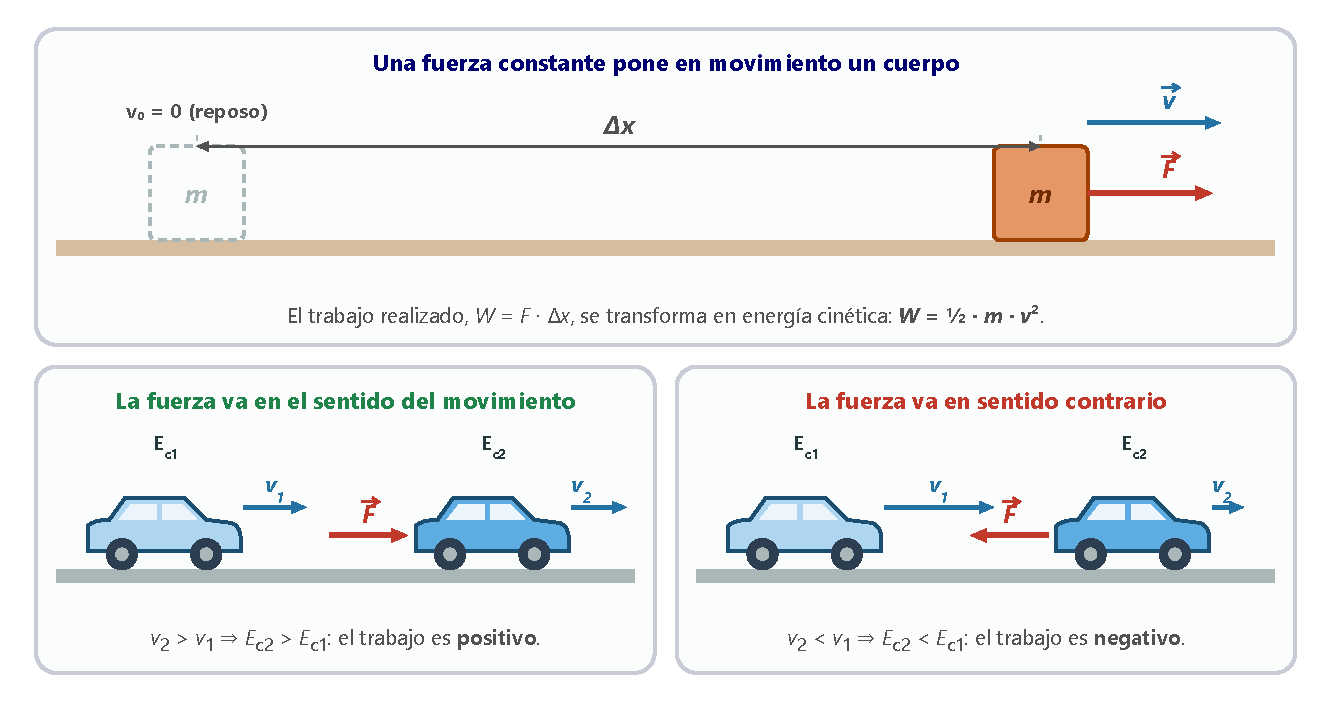
\includegraphics[width=\textwidth]{images/UD11/energia_cinetica}
    \caption{El trabajo realizado sobre un cuerpo se transforma en energía cinética.}
    \label{fig:energia_cinetica}
\end{figure}

\paragraph{¿Qué relación hay entre el trabajo y la variación de energía cinética?} Si un cuerpo ya se mueve y le aplicamos una fuerza, su velocidad puede aumentar o disminuir.

\begin{definition}[Teorema de la energía cinética]
    El trabajo realizado por la resultante de todas las fuerzas que actúan sobre un cuerpo es igual a la variación de su energía cinética:
    \[ W = E_{c2} - E_{c1} = \Delta E_c \]
\end{definition}

Si la fuerza resultante tiene el sentido del movimiento, la velocidad aumenta, \(E_{c2} > E_{c1}\), y el trabajo es \textbf{positivo}. Si tiene sentido contrario (por ejemplo, al frenar), la velocidad disminuye, \(E_{c2} < E_{c1}\), y el trabajo es \textbf{negativo}.

\begin{example}
    Una vagoneta de \qty{100}{\kg} se mueve en línea recta a \qty{2}{\m\per\s}. Le aplicamos una fuerza y, tras recorrer \qty{5}{\m}, su velocidad es de \qty{4}{\m\per\s}. Si no hay rozamiento, calcula el trabajo realizado y el valor de la fuerza.

    \(E_{c1} = \frac{1}{2} \cdot 100 \cdot 2^2 = \qty{200}{\joule}\); \quad \(E_{c2} = \frac{1}{2} \cdot 100 \cdot 4^2 = \qty{800}{\joule}\).
    \[ W = \Delta E_c = 800 - 200 = \textcolor{red}{\qty{600}{\joule}} \qquad F = \frac{W}{\Delta x} = \frac{600}{5} = \textcolor{red}{\qty{120}{\newton}} \]
\end{example}

\begin{exercise}
    Escribe la ecuación de dimensiones de la energía cinética y comprueba que coincide con la del trabajo. ¿Es una ecuación homogénea?
    \begin{solu}
        \([E_c] = [m] \cdot [v]^2 = \mathrm{M} \cdot (\mathrm{L \cdot T^{-1}})^2 = \textcolor{red}{\mathrm{M \cdot L^2 \cdot T^{-2}}}\), igual que la del trabajo: la ecuación \(W = \frac{1}{2} m v^2\) \textcolor{red}{es homogénea}.
    \end{solu}
\end{exercise}

\begin{exercise}
    Un cuerpo de \qty{50}{\kg} se mueve a \qty{2}{\m\per\s}. ¿Qué energía cinética tiene? ¿Cuánto aumentaría si se duplicara su masa? ¿Y si se duplicara su velocidad?
    \begin{solu}
        \(E_c = \frac{1}{2} \cdot 50 \cdot 2^2 = \textcolor{red}{\qty{100}{\joule}}\). Si se duplica la masa, la energía cinética \textcolor{red}{se duplica} (\qty{200}{\joule}); si se duplica la velocidad, \textcolor{red}{se cuadruplica} (\qty{400}{\joule}).
    \end{solu}
\end{exercise}

\begin{exercise}
    ¿Puede ser negativa la energía cinética de un cuerpo? ¿Y su variación?
    \begin{solu}
        La energía cinética \textcolor{red}{no puede ser negativa}: la masa es positiva y la velocidad está elevada al cuadrado. Su variación \textcolor{red}{sí puede ser negativa}, cuando el cuerpo pierde velocidad (por ejemplo, al frenar).
    \end{solu}
\end{exercise}

\begin{exercise}
    Calcula la energía cinética de un vehículo de \qty{500}{\kg} que circula a \qty{90}{\km\per\hour}.
    \begin{solu}
        \(v = \qty{90}{\km\per\hour} = \qty{25}{\m\per\s}\); \(E_c = \frac{1}{2} \cdot 500 \cdot 25^2 = \textcolor{red}{\qty{1.56e5}{\joule}}\).
    \end{solu}
\end{exercise}

\begin{exercise}
    Un vehículo de \qty{600}{\kg} que circula por una carretera recta y horizontal pasa de \qty{10}{\m\per\s} a \qty{20}{\m\per\s} en \qty{10}{\m}. Calcula la fuerza resultante que ha actuado sobre él.
    \begin{solu}
        \(E_{c1} = \frac{1}{2} \cdot 600 \cdot 10^2 = \qty{30000}{\joule}\); \(E_{c2} = \frac{1}{2} \cdot 600 \cdot 20^2 = \qty{120000}{\joule}\).
        \(W = \Delta E_c = \qty{90000}{\joule}\); \(F = \dfrac{W}{\Delta x} = \dfrac{90000}{10} = \textcolor{red}{\qty{9000}{\newton}}\).
    \end{solu}
\end{exercise}

\subsection{¿Puede un cuerpo en reposo tener energía mecánica? La energía potencial}

Un saltador de trampolín en lo alto de la plataforma está quieto, pero tiene energía: cuando salte, su peso realizará un trabajo y ganará velocidad.

\begin{definition}[Energía potencial]
    La \textbf{energía potencial}, \(E_p\), es la energía que tiene un cuerpo debido a la posición que ocupa, distinta de su posición de equilibrio.
\end{definition}

\paragraph{La energía potencial gravitatoria.} Cuando una roca de masa \(m\) cae desde una altura \(h\) (figura~\ref{fig:energia_potencial}), su peso y el desplazamiento tienen la misma dirección y sentido, así que el peso realiza un trabajo positivo:
\[ W = m \cdot g \cdot h \]
Este trabajo es igual a la \textbf{disminución} de la energía potencial: \(W = -\Delta E_p = E_{p1} - E_{p2}\). Solo podemos calcular diferencias de energía potencial, así que tomamos por convenio como nivel cero el suelo (\(h = 0\)). Entonces, \(E_{p2} = 0\) y \(W = E_{p1} = m \cdot g \cdot h\).

\begin{definition}[Energía potencial gravitatoria]
    La energía potencial gravitatoria de un cuerpo de masa \(m\) situado a una altura \(h\) sobre el nivel de referencia es:
    \[ E_p = m \cdot g \cdot h \]
\end{definition}

Para \textbf{subir} la roca desde el suelo hasta la altura \(h\), el peso y el desplazamiento tienen sentidos opuestos: el peso realiza un trabajo negativo, \(W = -m \cdot g \cdot h\), y nosotros tenemos que realizar un trabajo \(m \cdot g \cdot h\), que queda almacenado como energía potencial. Este trabajo \textbf{no depende del camino seguido}, sino solo de la diferencia de altura.

\begin{figure}[H]
    \centering
    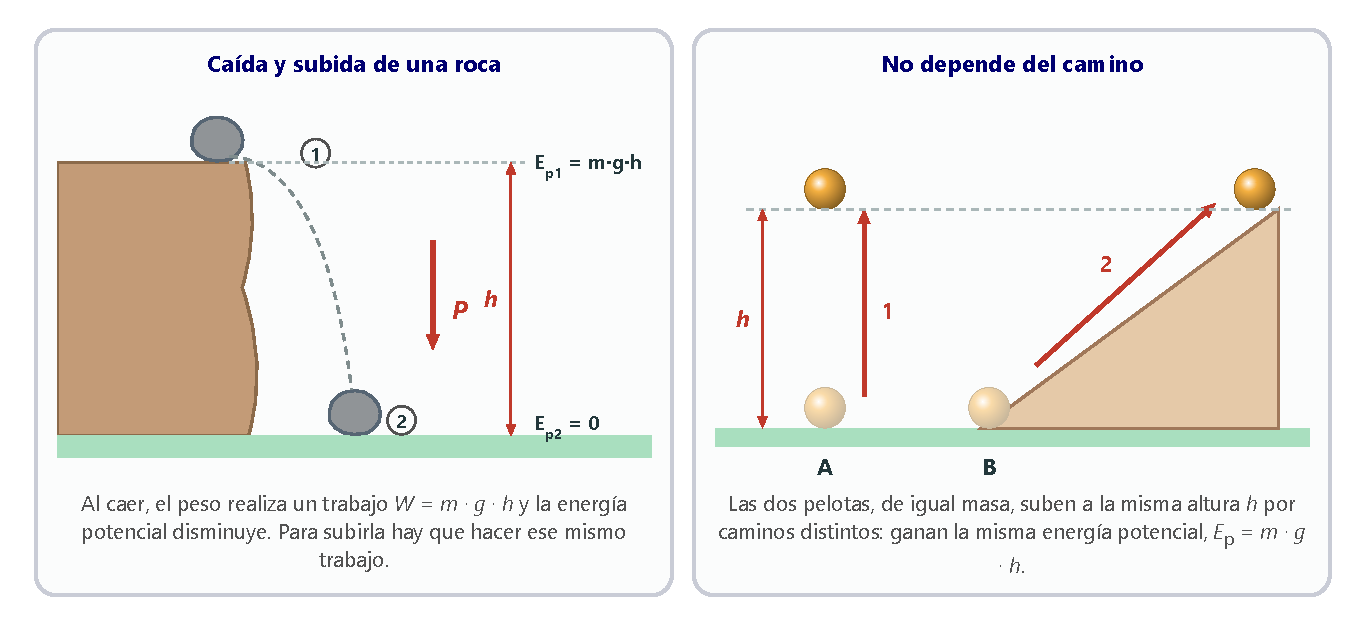
\includegraphics[width=\textwidth]{images/UD11/energia_potencial}
    \caption{La energía potencial gravitatoria depende solo de la altura.}
    \label{fig:energia_potencial}
\end{figure}

\paragraph{La energía potencial elástica.} Para estirar o comprimir un muelle una distancia \(x\) hay que aplicar una fuerza que cumple la \textbf{ley de Hooke}: \(F = k \cdot x\), donde \(k\) es la constante elástica del muelle (figura~\ref{fig:muelle}). El trabajo realizado no se convierte en energía cinética (el muelle se estira despacio) ni en energía potencial gravitatoria (el movimiento es horizontal): queda almacenado en el muelle deformado.

\begin{figure}[H]
    \centering
    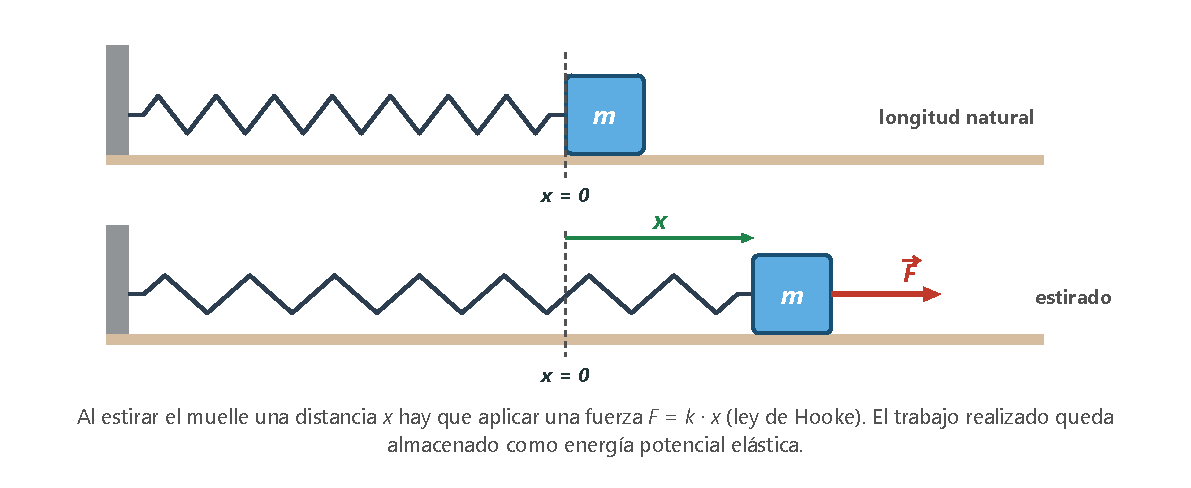
\includegraphics[width=0.85\textwidth]{images/UD11/muelle}
    \caption{Un muelle estirado almacena energía potencial elástica.}
    \label{fig:muelle}
\end{figure}

Como la fuerza no es constante, el trabajo se calcula como el área bajo la gráfica \(F\)--\(x\), que es un triángulo de base \(x\) y altura \(k \cdot x\):
\[ W = \frac{1}{2} \cdot x \cdot (k \cdot x) = \frac{1}{2} \cdot k \cdot x^2 \]

\begin{center}
    \begin{tikzpicture}
        \begin{axis}[grafica, width=7cm, height=5cm, xlabel={alargamiento, \(x\)}, ylabel={fuerza, \(F\)}, xmin=0, xmax=5.5, ymin=0, ymax=5.5, xticklabels={}, yticklabels={}]
            \addplot[mark=none, fill=red!20, draw=red!75!black, line width=1.4pt] coordinates {(0,0) (4,4) (4,0)};
            \node at (axis cs:2.4,0.6) {\small área \(= \frac{1}{2} \cdot b \cdot h\)};
            \node[anchor=west] at (axis cs:4.05,4) {\small \(F = k \cdot x\)};
        \end{axis}
    \end{tikzpicture}
\end{center}

\begin{definition}[Energía potencial elástica]
    La \textbf{energía potencial elástica} es la que tiene un cuerpo elástico (un muelle, una goma\ldots) cuando está estirado o comprimido. Si cumple la ley de Hooke:
    \[ E_p = \frac{1}{2} \cdot k \cdot x^2 \]
    Es proporcional al \textbf{cuadrado} de la deformación.
\end{definition}

\begin{example}
    Calcula la energía potencial elástica de un muelle de constante \qty{100}{\newton\per\m} comprimido \qty{4}{\cm} desde su longitud natural.
    \[ E_p = \frac{1}{2} \cdot k \cdot x^2 = \frac{1}{2} \cdot 100 \cdot (\num{0.04})^2 = \textcolor{red}{\qty{0.08}{\joule}} \]
\end{example}

\begin{exercise}
    Calcula la energía potencial de un saltador de trampolín de \qty{75}{\kg} situado a \qty{10}{\m} sobre el agua. ¿Qué trabajo realiza su peso cuando cae a la piscina?
    \begin{solu}
        \(E_p = m \cdot g \cdot h = 75 \cdot \num{9.8} \cdot 10 = \textcolor{red}{\qty{7350}{\joule}}\). El peso realiza ese mismo trabajo al caer: \(W = \textcolor{red}{\qty{7350}{\joule}}\).
    \end{solu}
\end{exercise}

\begin{exercise}
    Un cuerpo de \qty{10}{\kg} está a \qty{4}{\m} de altura. ¿Qué trabajo realiza su peso cuando cae hasta el suelo?
    \begin{solu}
        \(W = -\Delta E_p = m \cdot g \cdot h = 10 \cdot \num{9.8} \cdot 4 = \textcolor{red}{\qty{392}{\joule}}\).
    \end{solu}
\end{exercise}

\begin{exercise}
    Al estirar un muelle, la fuerza aumenta de forma proporcional al alargamiento, como en la gráfica. Calcula el trabajo realizado. ¿Qué energía potencial elástica ha adquirido el muelle?
    \begin{center}
        \begin{tikzpicture}
            \begin{axis}[grafica, width=6.5cm, height=4.2cm, xlabel={\(x\) (cm)}, ylabel={\(F\) (N)}, xmin=0, xmax=6, ymin=0, ymax=5, xtick={0,2,4,6}, ytick={0,2,4}]
                \addplot[mark=none, fill=red!20, draw=red!75!black, line width=1.4pt] coordinates {(0,0) (4,4) (4,0)};
            \end{axis}
        \end{tikzpicture}
    \end{center}
    \begin{solu}
        El trabajo es el área del triángulo: \(W = \frac{1}{2} \cdot \num{0.04} \cdot 4 = \textcolor{red}{\qty{0.08}{\joule}}\). Esa es la energía potencial elástica que ha adquirido el muelle: \(E_p = \textcolor{red}{\qty{0.08}{\joule}}\).
    \end{solu}
\end{exercise}

\begin{exercise}
    Un muelle de constante \qty{50}{\newton\per\m} se estira hasta que su energía potencial elástica es \qty{6.25e-2}{\joule}. ¿Cuánto se ha estirado? ¿Cuánto varía su energía potencial cuando vuelve a su longitud natural?
    \begin{solu}
        \(\num{6.25e-2} = \frac{1}{2} \cdot 50 \cdot x^2 \Rightarrow x^2 = \num{2.5e-3} \Rightarrow x = \textcolor{red}{\qty{0.05}{\m}} = \qty{5}{\cm}\).
        Al volver a su longitud natural, \(\Delta E_p = 0 - \num{6.25e-2} = \textcolor{red}{\qty{-6.25e-2}{\joule}}\).
    \end{solu}
\end{exercise}

\begin{exercise}
    Comprueba que la ecuación \(E_p = m \cdot g \cdot h\) es homogénea.
    \begin{solu}
        \([m \cdot g \cdot h] = \mathrm{M} \cdot \mathrm{L \cdot T^{-2}} \cdot \mathrm{L} = \mathrm{M \cdot L^2 \cdot T^{-2}}\), que son las dimensiones de una energía: \textcolor{red}{es homogénea}.
    \end{solu}
\end{exercise}

\subsection*{Actividades de consolidación: energía mecánica}

\begin{exercise}
    Indica si son verdaderas o falsas estas afirmaciones:
    \begin{enumerate}[label=\alph*)]
        \item La energía cinética depende de la masa del cuerpo y de su velocidad.
        \item Un cuerpo en reposo puede tener energía mecánica.
        \item Si B tiene la misma masa que A y el doble de velocidad, tiene el doble de energía cinética.
        \item La energía cinética de un cuerpo puede ser negativa.
        \item La variación de energía cinética puede ser negativa.
        \item La energía potencial elástica es proporcional al cuadrado de la deformación.
        \item El trabajo realizado por el peso es igual a la disminución de la energía potencial gravitatoria.
    \end{enumerate}
    \begin{solu}
        a) \textcolor{red}{V}. b) \textcolor{red}{V} (energía potencial). c) \textcolor{red}{F}: tiene cuatro veces más. d) \textcolor{red}{F}. e) \textcolor{red}{V}. f) \textcolor{red}{V}. g) \textcolor{red}{V}.
    \end{solu}
\end{exercise}

\begin{exercise}
    ¿Cuánto varía la energía cinética de un atleta de \qty{60}{\kg} cuando su velocidad pasa de \qty{1.5}{\m\per\s} a \qty{2.75}{\m\per\s}?
    \begin{solu}
        \(E_{c1} = \frac{1}{2} \cdot 60 \cdot \num{1.5}^2 = \qty{67.5}{\joule}\); \(E_{c2} = \frac{1}{2} \cdot 60 \cdot \num{2.75}^2 = \qty{226.9}{\joule}\); \(\Delta E_c = \textcolor{red}{\qty{159.4}{\joule}}\).
    \end{solu}
\end{exercise}

\begin{exercise}
    Un bloque de piedra de \qty{100}{\kg}, en reposo sobre un plano liso y horizontal, es empujado con una fuerza constante de \qty{25}{\newton} a lo largo de \qty{25}{\m}. Calcula la energía cinética y la velocidad que adquiere.
    \begin{solu}
        \(E_c = W = 25 \cdot 25 = \textcolor{red}{\qty{625}{\joule}}\); \(v = \sqrt{\dfrac{2 E_c}{m}} = \sqrt{\dfrac{2 \cdot 625}{100}} = \textcolor{red}{\qty{3.54}{\m\per\s}}\).
    \end{solu}
\end{exercise}

\begin{exercise}
    Un vehículo de \qty{500}{\kg} circula a \qty{100}{\km\per\hour} y frena hasta detenerse. ¿Cuánto varía su energía cinética? ¿Qué trabajo realiza la fuerza de frenado?
    \begin{solu}
        \(v = \qty{27.8}{\m\per\s}\); \(E_c = \frac{1}{2} \cdot 500 \cdot \num{27.8}^2 = \qty{1.93e5}{\joule}\). \(\Delta E_c = 0 - \num{1.93e5} = \textcolor{red}{\qty{-1.93e5}{\joule}}\), que es el trabajo de la fuerza de frenado: \(W = \textcolor{red}{\qty{-1.93e5}{\joule}}\).
    \end{solu}
\end{exercise}

\begin{exercise}
    Si el trabajo realizado por la fuerza resultante sobre un cuerpo es nulo, su energía cinética es: a) nula; b) constante.
    \begin{solu}
        \textcolor{red}{b) constante}, porque \(W = \Delta E_c = 0\).
    \end{solu}
\end{exercise}

\begin{exercise}
    Un halcón en vuelo tiene más energía cinética que un águila, aunque el águila tiene más masa. ¿Cómo es posible?
    \begin{solu}
        Porque la energía cinética depende del \textcolor{red}{cuadrado de la velocidad}: el halcón vuela mucho más rápido, y eso compensa su menor masa.
    \end{solu}
\end{exercise}

\begin{exercise}
    Un cuerpo de \qty{1}{\kg} se mueve a \qty{2}{\m\per\s}. ¿Qué trabajo hay que realizar sobre él para pararlo?
    \begin{solu}
        \(W = \Delta E_c = 0 - \frac{1}{2} \cdot 1 \cdot 2^2 = \textcolor{red}{\qty{-2}{\joule}}\): hay que quitarle \qty{2}{\joule} con una fuerza de sentido contrario al movimiento.
    \end{solu}
\end{exercise}

\begin{exercise}
    Una maleta de \qty{8}{\kg}, inicialmente en reposo, es empujada con una fuerza de \qty{16}{\newton} por un suelo horizontal sin rozamiento y se desplaza \qty{4}{\m}. Calcula: a) el trabajo de la fuerza; b) la variación de energía cinética; c) la velocidad final.
    \begin{solu}
        a) \(W = 16 \cdot 4 = \textcolor{red}{\qty{64}{\joule}}\). b) \(\Delta E_c = W = \textcolor{red}{\qty{64}{\joule}}\). c) \(v = \sqrt{\dfrac{2 \cdot 64}{8}} = \textcolor{red}{\qty{4}{\m\per\s}}\).
    \end{solu}
\end{exercise}

\begin{exercise}
    Un coche recorre \qty{2}{\km} por una carretera horizontal y su energía cinética aumenta \qty{20000}{\joule}. ¿Qué trabajo neto se ha realizado sobre él?
    \begin{solu}
        \(W = \Delta E_c = \textcolor{red}{\qty{20000}{\joule}}\) (es el trabajo de la fuerza resultante: el del motor menos el que se pierde por rozamiento).
    \end{solu}
\end{exercise}

\begin{exercise}
    ¿Cómo varía la energía potencial gravitatoria en un desplazamiento horizontal?
    \begin{solu}
        \textcolor{red}{No varía}, porque la altura es la misma.
    \end{solu}
\end{exercise}

\begin{exercise}
    En una escalera de peldaños de \qty{15}{\cm}, las posiciones 1, 2 y 3 están a \qty{0.15}{\m}, \qty{0.45}{\m} y \qty{0.75}{\m} del suelo. Un cuerpo A, de \qty{2}{\kg}, está en la posición 3, y un cuerpo B, de \qty{1}{\kg}, en la posición 1. a) ¿Qué energía potencial tiene cada uno? b) ¿Qué trabajo hay que hacer para subir B de la posición 1 a la 2? c) ¿Cuánto varía la energía potencial de A al bajar de la posición 3 a la 2?
    \begin{solu}
        a) \(E_{pA} = 2 \cdot \num{9.8} \cdot \num{0.75} = \textcolor{red}{\qty{14.7}{\joule}}\); \(E_{pB} = 1 \cdot \num{9.8} \cdot \num{0.15} = \textcolor{red}{\qty{1.47}{\joule}}\).
        b) \(W = 1 \cdot \num{9.8} \cdot (\num{0.45} - \num{0.15}) = \textcolor{red}{\qty{2.94}{\joule}}\).
        c) \(\Delta E_p = 2 \cdot \num{9.8} \cdot (\num{0.45} - \num{0.75}) = \textcolor{red}{\qty{-5.88}{\joule}}\).
    \end{solu}
\end{exercise}

\begin{exercise}
    Una grúa eleva una viga de \qty{100}{\kg} desde el suelo hasta \qty{20}{\m} de altura. a) ¿Qué trabajo realiza? b) ¿Qué energía potencial tiene la viga en el suelo y a \qty{20}{\m}? c) ¿A qué equivale su variación de energía potencial?
    \begin{solu}
        a) \(W = 100 \cdot \num{9.8} \cdot 20 = \textcolor{red}{\qty{19600}{\joule}}\). b) En el suelo, \textcolor{red}{\qty{0}{\joule}}; a \qty{20}{\m}, \textcolor{red}{\qty{19600}{\joule}}. c) \textcolor{red}{Al trabajo realizado} por la grúa para subirla.
    \end{solu}
\end{exercise}

\begin{exercise}
    Queremos subir un cuerpo de \qty{10}{\kg} desde el suelo. a) ¿Qué energía potencial tiene en el suelo? b) ¿Y a \qty{4}{\m} de altura? c) ¿Qué trabajo hay que hacer para subirlo? d) ¿Cuándo es negativa la variación de energía potencial?
    \begin{solu}
        a) \textcolor{red}{\qty{0}{\joule}}. b) \(E_p = 10 \cdot \num{9.8} \cdot 4 = \textcolor{red}{\qty{392}{\joule}}\). c) \(W = \Delta E_p = \textcolor{red}{\qty{392}{\joule}}\). d) Cuando el cuerpo \textcolor{red}{baja}: la energía potencial final es menor que la inicial.
    \end{solu}
\end{exercise}

\begin{exercise}
    Calcula la energía potencial elástica de un muelle de constante \qty{2000}{\newton\per\m} estirado \qty{2}{\cm}.
    \begin{solu}
        \(E_p = \frac{1}{2} \cdot 2000 \cdot (\num{0.02})^2 = \textcolor{red}{\qty{0.4}{\joule}}\).
    \end{solu}
\end{exercise}

\begin{exercise}
    Dos pelotas iguales, A y B, suben a la misma altura \(h\): A, verticalmente; B, rodando por una rampa (figura~\ref{fig:energia_potencial}). a) ¿Qué energía potencial adquiere cada una? b) ¿Qué trabajo se ha hecho para subirlas? c) ¿Qué conclusión se obtiene?
    \begin{solu}
        a) Las dos, \textcolor{red}{la misma}: \(E_p = m \cdot g \cdot h\). b) El mismo, \(W = m \cdot g \cdot h\) (sin rozamiento). c) El trabajo para subir un cuerpo \textcolor{red}{no depende del camino}, solo de la altura.
    \end{solu}
\end{exercise}

\begin{exercise}
    Calcula la energía potencial elástica de un muelle de constante \qty{100}{\newton\per\m} comprimido \qty{5}{\cm}.
    \begin{solu}
        \(E_p = \frac{1}{2} \cdot 100 \cdot (\num{0.05})^2 = \textcolor{red}{\qty{0.125}{\joule}}\).
    \end{solu}
\end{exercise}

\begin{exercise}
    La fuerza de la gráfica no es constante. Calcula el trabajo que realiza entre \(x = 0\) y \(x = \qty{8}{\m}\).
    \begin{center}
        \begin{tikzpicture}
            \begin{axis}[grafica, width=8cm, height=4.4cm, xlabel={\(x\) (m)}, ylabel={\(F\) (N)}, xmin=0, xmax=8.6, ymin=0, ymax=75, xtick={0,2,...,8}, ytick={0,20,40,60}]
                \addplot[mark=none, fill=red!20, draw=red!75!black, line width=1.4pt] coordinates {(0,0) (2,60) (4,60) (8,0)};
            \end{axis}
        \end{tikzpicture}
    \end{center}
    \begin{solu}
        El trabajo es el área bajo la gráfica: un triángulo, un rectángulo y otro triángulo.
        \(W = \frac{1}{2} \cdot 2 \cdot 60 + 2 \cdot 60 + \frac{1}{2} \cdot 4 \cdot 60 = 60 + 120 + 120 = \textcolor{red}{\qty{300}{\joule}}\).
    \end{solu}
\end{exercise}

\begin{exercise}
    Una joven de \qty{65}{\kg} sube a una torre de \qty{93}{\m}. a) ¿Qué trabajo realiza? b) ¿Qué energía potencial tiene arriba?
    \begin{solu}
        a) \(W = 65 \cdot \num{9.8} \cdot 93 = \textcolor{red}{\qty{59241}{\joule}}\). b) La misma: \(E_p = \textcolor{red}{\qty{59241}{\joule}}\).
    \end{solu}
\end{exercise}

\begin{exercise}
    Un cuerpo de \qty{8}{\kg} cae desde \qty{20}{\m}. ¿Cuánto varía su energía potencial? ¿Qué trabajo realiza el peso?
    \begin{solu}
        \(\Delta E_p = 0 - 8 \cdot \num{9.8} \cdot 20 = \textcolor{red}{\qty{-1568}{\joule}}\); el peso realiza un trabajo \(W = -\Delta E_p = \textcolor{red}{\qty{1568}{\joule}}\).
    \end{solu}
\end{exercise}

%========================================================================================
\section[Conservación de la energía mecánica]{El principio de conservación de la energía mecánica}
%========================================================================================

\begin{definition}[Energía mecánica]
    La \textbf{energía mecánica}, \(E_m\), es la suma de la energía cinética y la energía potencial de un cuerpo:
    \[ E_m = E_c + E_p \]
\end{definition}

\subsection{¿Cómo se transforma la energía potencial en cinética y viceversa?}

Una niña de \qty{25}{\kg} está sentada, en reposo, en lo alto de un tobogán de \qty{2}{\m} (figura~\ref{fig:conservacion}). No tiene energía cinética, y su energía potencial es \(E_p = 25 \cdot \num{9.8} \cdot 2 = \qty{490}{\joule}\). Mientras baja, su energía potencial disminuye y su energía cinética aumenta. A mitad de altura (\(h = \qty{1}{\m}\)), \(E_p = \qty{245}{\joule}\) y \(E_c = \qty{245}{\joule}\); al llegar abajo, toda la energía potencial se ha transformado en cinética: \(E_c = \qty{490}{\joule}\). En todo momento, la suma de las dos es \qty{490}{\joule}.

\begin{definition}[Principio de conservación de la energía mecánica]
    Si no hay rozamiento, la suma de la energía cinética y la energía potencial de un cuerpo permanece constante en todos los puntos de su trayectoria:
    \[ E_m = E_c + E_p = \text{constante} \]
\end{definition}

\begin{figure}[H]
    \centering
    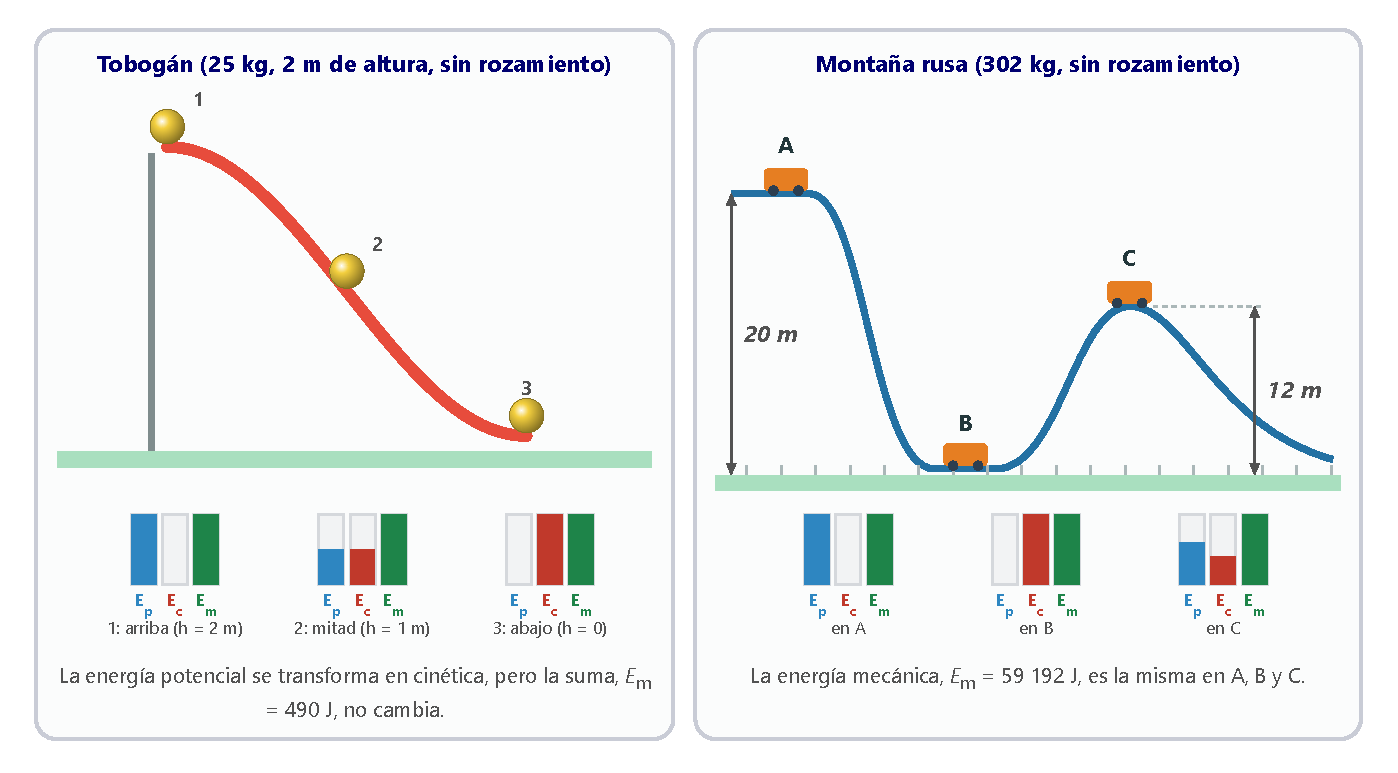
\includegraphics[width=\textwidth]{images/UD11/conservacion}
    \caption{Conservación de la energía mecánica en un tobogán y en una montaña rusa.}
    \label{fig:conservacion}
\end{figure}

Gracias a este principio podemos calcular velocidades sin conocer las fuerzas. Por ejemplo, la velocidad de la niña al final del tobogán:
\[ E_c = \frac{1}{2} \cdot m \cdot v^2 \quad\Rightarrow\quad v = \sqrt{\frac{2 E_c}{m}} = \sqrt{\frac{2 \cdot 490}{25}} = \qty{6.26}{\m\per\s} \]
Si toda la energía potencial se transforma en cinética, \(m \cdot g \cdot h = \frac{1}{2} \cdot m \cdot v^2\), y la velocidad final es \(v = \sqrt{2 \cdot g \cdot h}\): no depende de la masa.

\subsection{Aplicaciones del principio de conservación de la energía mecánica}

\begin{example}
    \textbf{Viaje en caída libre.} En una atracción, el vehículo y su pasajero (\qty{248}{\kg} en total) suben hasta \qty{50}{\m} y se dejan caer. Despreciando el rozamiento, calcula la energía mecánica y la velocidad con que llegan abajo, antes de frenar.

    Arriba, en reposo: \(E_m = E_p = 248 \cdot \num{9.8} \cdot 50 = \textcolor{red}{\qty{121520}{\joule}}\). Abajo, toda es cinética:
    \[ v = \sqrt{\frac{2 E_c}{m}} = \sqrt{\frac{2 \cdot 121520}{248}} = \textcolor{red}{\qty{31.3}{\m\per\s}} \quad (\text{más de } \qty{110}{\km\per\hour}) \]
\end{example}

\begin{example}
    \textbf{Viaje en montaña rusa.} Un vagón con su pasajero (\qty{302}{\kg}) parte del reposo en el punto A, a \qty{20}{\m} de altura, baja hasta el punto B, al nivel del suelo, y sube al punto C, a \qty{12}{\m} (figura~\ref{fig:conservacion}). Sin rozamiento, calcula la energía mecánica y las energías cinética y potencial en B y en C.

    En A: \(E_m = E_p = 302 \cdot \num{9.8} \cdot 20 = \textcolor{red}{\qty{59192}{\joule}}\), y se conserva en todo el recorrido.

    En B (\(h = 0\)): \(E_p = 0\) y \(E_c = \textcolor{red}{\qty{59192}{\joule}}\), el valor máximo.

    En C: \(E_p = 302 \cdot \num{9.8} \cdot 12 = \textcolor{red}{\qty{35515}{\joule}}\); \(E_c = 59192 - 35515 = \textcolor{red}{\qty{23677}{\joule}}\).
\end{example}

\begin{exercise}
    Un cuerpo de \qty{1}{\kg} se deja caer desde una torre. ¿Qué tipo de energía tiene en el momento en que está a \qty{10}{\m} del suelo: potencial, cinética o ambas?
    \begin{solu}
        \textcolor{red}{Ambas}: potencial, porque aún está a cierta altura, y cinética, porque ya se mueve. Al soltarlo solo tenía energía potencial, y al llegar al suelo solo tendrá cinética.
    \end{solu}
\end{exercise}

\begin{exercise}
    Un bloque de \qty{2}{\kg} se desliza sin rozamiento a \qty{2}{\m\per\s} y choca contra un muelle de constante \qty{100}{\newton\per\m}. ¿Cuánto se comprime el muelle?
    \begin{solu}
        Toda la energía cinética se transforma en potencial elástica:
        \(\frac{1}{2} \cdot 2 \cdot 2^2 = \frac{1}{2} \cdot 100 \cdot x^2 \Rightarrow 4 = 50 \, x^2 \Rightarrow x = \textcolor{red}{\qty{0.28}{\m}} = \qty{28}{\cm}\).
    \end{solu}
\end{exercise}

\begin{exercise}
    En la atracción de caída libre del ejemplo anterior, ¿qué energía potencial y cinética tiene el vehículo cuando está a \qty{10}{\m} del suelo? ¿Y qué energía mecánica?
    \begin{solu}
        \(E_p = 248 \cdot \num{9.8} \cdot 10 = \textcolor{red}{\qty{24304}{\joule}}\); \(E_c = 121520 - 24304 = \textcolor{red}{\qty{97216}{\joule}}\). La energía mecánica es la misma que en todo el recorrido: \(E_m = \textcolor{red}{\qty{121520}{\joule}}\).
    \end{solu}
\end{exercise}

\subsection*{Actividades de consolidación: conservación de la energía mecánica}

\begin{exercise}
    ¿En qué se transforma la energía potencial elástica de un juguete de cuerda?
    \begin{solu}
        En \textcolor{red}{energía cinética} del juguete (y, por los rozamientos, en energía térmica).
    \end{solu}
\end{exercise}

\begin{exercise}
    Un cuerpo en reposo a cierta altura se deja caer libremente. a) ¿Qué energía tiene al principio? b) ¿Qué ocurre con su energía cinética durante la caída? c) ¿Qué energía tiene al llegar al suelo?
    \begin{solu}
        a) Solo \textcolor{red}{potencial gravitatoria}. b) \textcolor{red}{Aumenta}, a medida que disminuye la potencial. c) Solo \textcolor{red}{cinética}.
    \end{solu}
\end{exercise}

\begin{exercise}
    Un péndulo tiene una masa de \qty{2}{\kg} y un hilo de \qty{0.5}{\m}. a) ¿Qué trabajo hay que hacer para llevarlo desde su posición de equilibrio hasta la horizontal? b) Si se suelta desde la horizontal, ¿con qué velocidad pasa por la posición de equilibrio?
    \begin{solu}
        a) La bola sube una altura igual a la longitud del hilo: \(W = m \cdot g \cdot h = 2 \cdot \num{9.8} \cdot \num{0.5} = \textcolor{red}{\qty{9.8}{\joule}}\).
        b) \(\frac{1}{2} \cdot m \cdot v^2 = \qty{9.8}{\joule} \Rightarrow v = \sqrt{\dfrac{2 \cdot \num{9.8}}{2}} = \textcolor{red}{\qty{3.13}{\m\per\s}}\).
    \end{solu}
\end{exercise}

\begin{exercise}
    Un cuerpo de \qty{10}{\kg} se lanza verticalmente hacia arriba a \qty{25}{\m\per\s}. Aplicando la conservación de la energía, calcula la altura máxima que alcanza.
    \begin{solu}
        \(\frac{1}{2} \cdot m \cdot v^2 = m \cdot g \cdot h \Rightarrow h = \dfrac{v^2}{2g} = \dfrac{25^2}{2 \cdot \num{9.8}} = \textcolor{red}{\qty{31.9}{\m}}\).
    \end{solu}
\end{exercise}

\begin{exercise}
    Un cuerpo de \qty{100}{\gram}, sujeto a un muelle de constante \qty{200}{\newton\per\m}, está apoyado en un plano horizontal sin rozamiento. Lo separamos \qty{10}{\cm} de su posición de equilibrio y lo soltamos. a) ¿Qué energía potencial tiene al principio? b) ¿Cuál es su energía mecánica? c) ¿Con qué velocidad pasa por la posición de equilibrio?
    \begin{solu}
        a) \(E_p = \frac{1}{2} \cdot 200 \cdot \num{0.1}^2 = \textcolor{red}{\qty{1}{\joule}}\). b) \(E_m = \textcolor{red}{\qty{1}{\joule}}\) durante todo el movimiento.
        c) \(\frac{1}{2} \cdot \num{0.1} \cdot v^2 = 1 \Rightarrow v = \sqrt{20} = \textcolor{red}{\qty{4.47}{\m\per\s}}\).
    \end{solu}
\end{exercise}

\begin{exercise}
    Por una presa con un desnivel de \qty{65}{\m} caen \qty{250}{\cubic\m} de agua por minuto. ¿Cuánta energía puede proporcionar el agua cada minuto? ¿Qué potencia supone?
    \begin{solu}
        \(m = \qty{250000}{\kg}\); \(E_p = 250000 \cdot \num{9.8} \cdot 65 = \textcolor{red}{\qty{1.6e8}{\joule}}\) por minuto.
        \(P = \dfrac{\num{1.6e8}}{60} = \textcolor{red}{\qty{2.7e6}{\watt}} = \qty{2.7}{\mega\watt}\).
    \end{solu}
\end{exercise}

\begin{exercise}
    Un cuerpo de \qty{10}{\kg} cae desde \qty{20}{\m}. a) ¿Qué energía potencial tiene a \qty{10}{\m} de altura? b) ¿Qué velocidad tiene en ese instante? c) ¿Qué trabajo realiza el peso hasta que llega al suelo? d) ¿Con qué velocidad llega al suelo?
    \begin{solu}
        a) \(E_p = 10 \cdot \num{9.8} \cdot 10 = \textcolor{red}{\qty{980}{\joule}}\).
        b) \(E_m = 10 \cdot \num{9.8} \cdot 20 = \qty{1960}{\joule}\), así que \(E_c = 1960 - 980 = \qty{980}{\joule}\) y \(v = \sqrt{\dfrac{2 \cdot 980}{10}} = \textcolor{red}{\qty{14}{\m\per\s}}\).
        c) \(W = m \cdot g \cdot h = \textcolor{red}{\qty{1960}{\joule}}\). d) \(v = \sqrt{\dfrac{2 \cdot 1960}{10}} = \textcolor{red}{\qty{19.8}{\m\per\s}}\).
    \end{solu}
\end{exercise}

\begin{exercise}
    Se deja caer una bola de \qty{4}{\kg} desde el punto A de una rampa, a \qty{2}{\m} de altura. La rampa baja hasta un tramo horizontal (puntos B y C, a nivel del suelo) y vuelve a subir. a) ¿Qué energía tiene en B y en C? b) Si no hay rozamiento, ¿qué altura alcanza en la rampa de subida?
    \begin{solu}
        a) En B y en C solo tiene \textcolor{red}{energía cinética}, igual a la potencial que tenía en A: \(E_c = 4 \cdot \num{9.8} \cdot 2 = \textcolor{red}{\qty{78.4}{\joule}}\).
        b) Sube hasta la \textcolor{red}{misma altura}, \qty{2}{\m}, porque la energía mecánica se conserva.
    \end{solu}
\end{exercise}

%========================================================================================
\section[Conservación de la energía total]{El principio general de conservación de la energía total}
%========================================================================================

Si dejamos caer una canica desde el borde de un cuenco, su energía potencial se transforma en cinética al bajar, y la cinética otra vez en potencial al subir por el otro lado. ¿Se repite indefinidamente? La experiencia dice que no: en cada oscilación la canica sube un poco menos, hasta que se para en el fondo (figura~\ref{fig:rozamiento_energia}).

En esta experiencia interviene una fuerza que no habíamos tenido en cuenta: la \textbf{fuerza de rozamiento}. Su trabajo es siempre negativo, así que la energía mecánica disminuye.

\begin{definition}[Trabajo de las fuerzas de rozamiento]
    El trabajo de las fuerzas de rozamiento es igual a la variación de energía mecánica del sistema:
    \[ W_{\text{roz}} = -F_{\text{roz}} \cdot \Delta x = E_{m,\text{final}} - E_{m,\text{inicial}} < 0 \]
\end{definition}

¿Significa esto que se ha perdido energía? No: lo que se ha perdido es \textbf{capacidad para realizar trabajo}. La energía mecánica se ha transformado en energía térmica, que calienta un poco la canica, el cuenco y el aire. Si tenemos en cuenta todas las formas de energía, se cumple una de las leyes más importantes de la naturaleza:

\begin{definition}[Principio de conservación de la energía]
    La energía ni se crea ni se destruye, solo se transforma: en todos los procesos hay intercambios de energía, pero la \textbf{energía total se mantiene constante}.
\end{definition}

\begin{figure}[H]
    \centering
    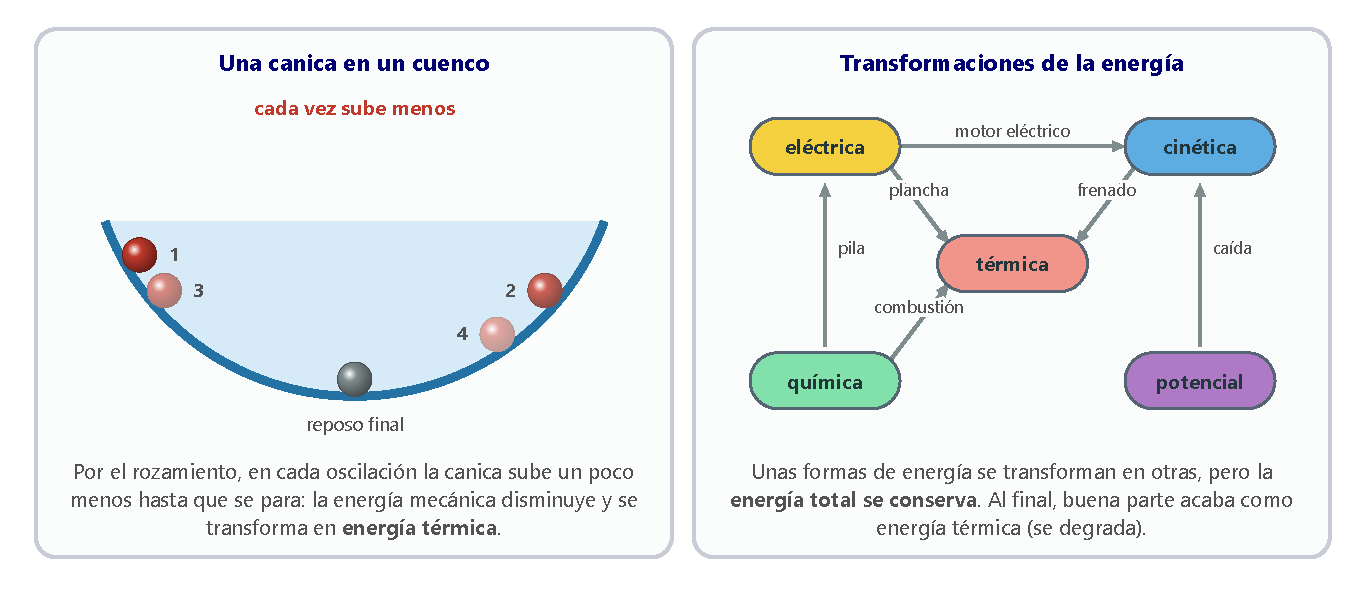
\includegraphics[width=\textwidth]{images/UD11/rozamiento_energia}
    \caption{El rozamiento transforma la energía mecánica en térmica. La energía total se conserva.}
    \label{fig:rozamiento_energia}
\end{figure}

\begin{example}
    ¿Cómo se transforma la energía cuando un futbolista golpea un balón?

    La \textcolor{red}{energía química} de los músculos se transforma en \textcolor{red}{energía cinética} de la pierna y, al golpear, del balón (parte se desprende como calor en los músculos). Mientras rueda, el rozamiento con el césped y el aire transforma su energía cinética en \textcolor{red}{energía térmica}, hasta que se para. La energía no se ha perdido: se ha transformado.
\end{example}

\begin{example}
    Un proyectil de \qty{e-3}{\kg} atraviesa un tablón: entra a \qty{300}{\m\per\s} y sale a \qty{200}{\m\per\s}. a) ¿Qué trabajo ha realizado la fuerza de rozamiento? b) ¿Se ha perdido energía?

    a) \(E_{m,\text{inicial}} = \frac{1}{2} \cdot \num{e-3} \cdot 300^2 = \qty{45}{\joule}\); \(E_{m,\text{final}} = \frac{1}{2} \cdot \num{e-3} \cdot 200^2 = \qty{20}{\joule}\).
    \[ W_{\text{roz}} = E_{m,\text{final}} - E_{m,\text{inicial}} = 20 - 45 = \textcolor{red}{\qty{-25}{\joule}} \]
    b) \textcolor{red}{No}: se ha perdido capacidad de realizar trabajo. Los \qty{25}{\joule} se han transformado en energía térmica (el proyectil y la madera se calientan).
\end{example}

\subsection{¿Una forma de energía se puede transformar en otra?}

Sí: en una plancha, la energía eléctrica se transforma en térmica; cuando un coche frena, la cinética se transforma en térmica; en una pila, la química se transforma en eléctrica; en un motor eléctrico, la eléctrica se transforma en cinética\ldots{} La energía total siempre se conserva, pero en estas transformaciones \textbf{se degrada}, pierde calidad: cualquier forma de energía puede transformarse \emph{íntegramente} en calor, pero el calor \emph{no} puede transformarse íntegramente en otra forma de energía. Por eso tiene sentido hablar de \emph{ahorrar} energía.

\begin{exercise}
    ¿Es correcto decir que en un proceso se ha perdido energía? ¿Y que se ha perdido capacidad para realizar trabajo?
    \begin{solu}
        \textcolor{red}{No} es correcto decir que se ha perdido energía, porque la energía total se conserva. \textcolor{red}{Sí} es correcto decir que se ha perdido capacidad para realizar trabajo: la energía se ha degradado, transformándose en energía térmica.
    \end{solu}
\end{exercise}

\begin{exercise}
    Distingue entre energía mecánica y energía total.
    \begin{solu}
        La \textcolor{red}{energía mecánica} es la suma de las energías cinética y potencial. La \textcolor{red}{energía total} es la suma de todas las formas de energía (mecánica, térmica, química, eléctrica\ldots).
    \end{solu}
\end{exercise}

\begin{exercise}
    Una bola se suelta desde el punto A de una rampa con forma de U y debería llegar al punto B, al otro lado y a la misma altura. ¿Llega hasta B? ¿No se cumple el principio de conservación de la energía mecánica?
    \begin{solu}
        Sin rozamiento llegaría justo hasta B. En la práctica siempre hay \textcolor{red}{rozamiento}, que transforma parte de la energía mecánica en térmica: la bola \textcolor{red}{sube un poco menos} en cada recorrido. La energía mecánica no se conserva, pero la \textcolor{red}{energía total sí}.
    \end{solu}
\end{exercise}

\begin{exercise}
    Describe las transformaciones de energía que se producen en una lámpara.
    \begin{solu}
        La \textcolor{red}{energía eléctrica} se transforma en \textcolor{red}{energía luminosa} y en \textcolor{red}{energía térmica} (la lámpara se calienta).
    \end{solu}
\end{exercise}

\begin{exercise}
    Un coche frena y se detiene. ¿Se ha perdido su energía cinética?
    \begin{solu}
        \textcolor{red}{No}: se ha transformado en \textcolor{red}{energía térmica} en los frenos, los neumáticos y el asfalto.
    \end{solu}
\end{exercise}

\begin{exercise}
    Pon un ejemplo de transformación de: a) energía térmica en mecánica; b) energía eléctrica en mecánica; c) energía eléctrica en química.
    \begin{solu}
        a) Una \textcolor{red}{máquina térmica} (motor de un coche, máquina de vapor). b) Un \textcolor{red}{motor eléctrico} (ventilador, tren eléctrico). c) La \textcolor{red}{electrólisis} o la carga de una batería.
    \end{solu}
\end{exercise}

\subsection*{Actividades de consolidación: conservación de la energía total}

\begin{exercise}
    Enuncia el principio general de conservación de la energía.
    \begin{solu}
        La energía \textcolor{red}{ni se crea ni se destruye, solo se transforma}: en todos los procesos hay intercambios de energía, pero la energía total se mantiene constante.
    \end{solu}
\end{exercise}

\begin{exercise}
    ¿Qué transformaciones de energía tienen lugar en una estufa eléctrica? ¿Y en un aerogenerador?
    \begin{solu}
        En la estufa, la energía \textcolor{red}{eléctrica se transforma en térmica}. En el aerogenerador, la energía \textcolor{red}{cinética del viento se transforma en eléctrica}.
    \end{solu}
\end{exercise}

\begin{exercise}
    Una bala de \qty{15}{\gram} entra a \qty{450}{\m\per\s} en una tabla de \qty{7}{\cm} de espesor. Si la tabla opone una fuerza de rozamiento de \qty{1200}{\newton}, ¿con qué velocidad sale?
    \begin{solu}
        \(E_{c,\text{inicial}} = \frac{1}{2} \cdot \num{0.015} \cdot 450^2 = \qty{1518.75}{\joule}\); \(W_{\text{roz}} = -1200 \cdot \num{0.07} = \qty{-84}{\joule}\).
        \(E_{c,\text{final}} = \num{1518.75} - 84 = \qty{1434.75}{\joule} \Rightarrow v = \sqrt{\dfrac{2 \cdot \num{1434.75}}{\num{0.015}}} = \textcolor{red}{\qty{437}{\m\per\s}}\).
    \end{solu}
\end{exercise}

\begin{exercise}
    ¿Por qué se calienta el cargador de un ordenador portátil o de un móvil cuando está enchufado?
    \begin{solu}
        Porque parte de la \textcolor{red}{energía eléctrica se transforma en energía térmica}: ninguna transformación de energía tiene un rendimiento del \qty{100}{\percent}.
    \end{solu}
\end{exercise}


%------------------------------------------------


    \chapterimage{images/portada_cabeceras/cabecera_UD12}
    \chapter{El calor: una forma de transferir energía}

    %! Author = crist
%! Date = 26/10/2026

\spacing{1.3}
%----------------------------------------------------------------------------------------
%	UNIDAD 12: EL CALOR, UNA FORMA DE TRANSFERIR ENERGÍA (4.º ESO)
%   Figuras: images/UD12/*.pdf (fuente HTML en images/UD12/html, SVG en images/UD12/svg)
%   Gráficas de calentamiento con pgfplots: estilo «grafica», definido al inicio de la UD1/UD7.
%   Datos usados en toda la unidad: c(agua) = 4180 J/(kg·°C); c(hielo) = 2100 J/(kg·°C);
%   L_f(agua) = 3,35·10^5 J/kg; L_v(agua) = 2,2·10^6 J/kg; T(K) = t(°C) + 273; 1 cal = 4,18 J.
%----------------------------------------------------------------------------------------
\DeclareSIUnit\cunit{\joule\per\kilogram\per\degreeCelsius} % J/(kg·°C), capacidad calorífica específica

% Mapa conceptual del tema (fuente en images/mapas_conceptuales/html/temas.js)
\begin{figure}[H]
    \centering
    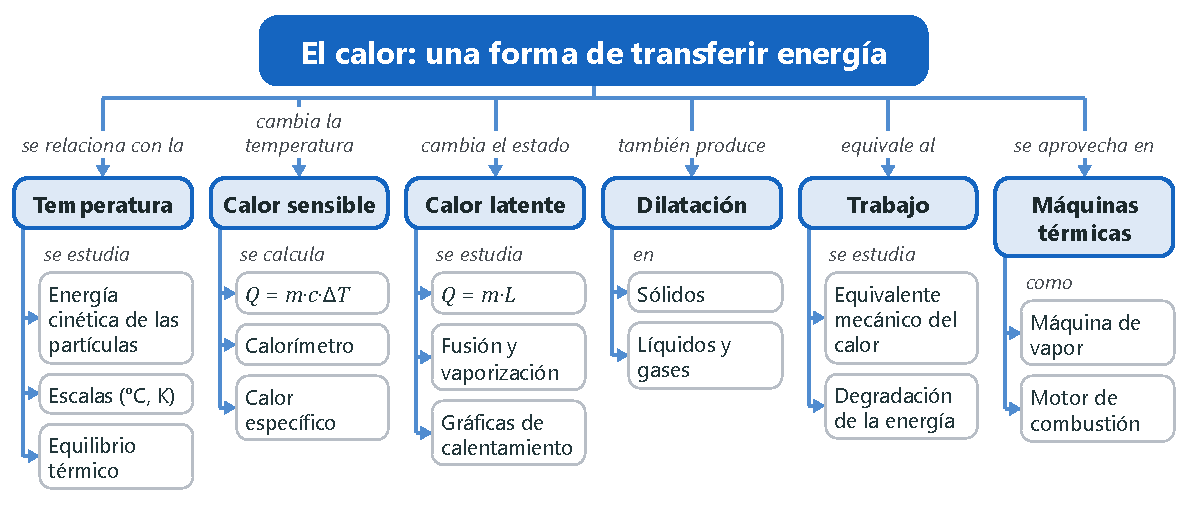
\includegraphics[width=\textwidth]{images/mapas_conceptuales/mapa_UD12}
\end{figure}

%========================================================================================
%\section*{Para empezar: el Sol, una fuente de energía renovable}
%\addcontentsline{toc}{section}{Para empezar: el Sol, una fuente de energía renovable}
%========================================================================================
%
%Casi toda la energía que mueve la «maquinaria» de la Tierra procede del Sol. Su radiación calienta la atmósfera, los océanos y los continentes; produce los vientos; evapora el agua y pone en marcha su ciclo; permite que las plantas realicen la fotosíntesis y, hace millones de años, dio lugar a los combustibles fósiles que hoy usamos en industrias, transportes y hogares.
%
%La humanidad ha aprovechado la energía solar desde siempre, y hoy lo hace de dos formas principales: las \textbf{células fotovoltaicas} transforman la luz del Sol en energía eléctrica, y los \textbf{colectores solares térmicos} la transforman en energía térmica para calentar agua o edificios. La energía solar es \textbf{renovable}, porque se regenera de forma natural, y prácticamente \textbf{inagotable} a escala humana: el Sol seguirá brillando miles de millones de años.
%
%Garantizar a todo el mundo el acceso a una energía asequible, fiable y moderna es el objetivo del \textbf{ODS 7} (\emph{Energía asequible y no contaminante}). Sus metas son aumentar la proporción de energías renovables, duplicar la mejora de la eficiencia energética y fomentar la investigación y la inversión en energías limpias.
%
%En la unidad anterior vimos que la energía se transfiere entre los cuerpos mediante el \textbf{trabajo}. En esta estudiaremos la otra forma de transferir energía, el \textbf{calor}: qué efectos produce (cambios de temperatura, cambios de estado, dilatación), cómo se relaciona con el trabajo y cómo las máquinas térmicas transforman la energía térmica en movimiento.
%
%\begin{exercise}
%    ¿Te parece adecuado el título «El Sol, una fuente de energía renovable e inagotable»? Razona tu respuesta.
%    \begin{solu}
%        \textcolor{red}{Sí}: la energía del Sol se renueva continuamente de forma natural y, a escala de la historia humana, no se agota, pues el Sol seguirá emitiendo energía durante miles de millones de años.
%    \end{solu}
%\end{exercise}
%
%\begin{exercise}
%    Explica tres maneras en las que el Sol influye en el funcionamiento de la naturaleza en la Tierra.
%    \begin{solu}
%        Por ejemplo: \textcolor{red}{calienta la atmósfera, los océanos y los continentes}; origina los \textcolor{red}{vientos} (por las diferencias de temperatura entre unas zonas y otras); pone en marcha el \textcolor{red}{ciclo del agua}; permite la \textcolor{red}{fotosíntesis} y, con ella, el crecimiento de las plantas, que son la base de las cadenas alimentarias.
%    \end{solu}
%\end{exercise}
%
%\begin{exercise}
%    ¿Cómo influyó el Sol en el pasado en la energía que usamos hoy?
%    \begin{solu}
%        La energía del Sol, captada por los seres vivos mediante la fotosíntesis hace millones de años, quedó almacenada en sus restos, que se transformaron en los \textcolor{red}{combustibles fósiles} (carbón, petróleo y gas natural).
%    \end{solu}
%\end{exercise}
%
%\begin{exercise}
%    ¿Por qué se dice que la energía solar es renovable? ¿Es lo mismo «renovable» que «no contaminante»?
%    \begin{solu}
%        Es \textcolor{red}{renovable porque se regenera de forma natural} y su uso no la agota. \textcolor{red}{No es lo mismo}: una fuente es renovable si no se agota, y es poco contaminante si su uso no emite sustancias perjudiciales. La energía solar cumple las dos condiciones durante su uso, aunque fabricar los paneles sí tiene un impacto ambiental.
%    \end{solu}
%\end{exercise}
%
%\begin{exercise}
%    ¿Qué transformación de energía se produce en una célula fotovoltaica? ¿Y en un colector solar térmico?
%    \begin{solu}
%        En la célula fotovoltaica, la energía de la luz se transforma en \textcolor{red}{energía eléctrica}. En el colector solar térmico, se transforma en \textcolor{red}{energía térmica} (calienta un fluido, normalmente agua).
%    \end{solu}
%\end{exercise}
%
%\begin{exercise}
%    Debatid en clase cómo puede contribuir la energía solar a lograr el ODS 7.
%    \begin{solu}
%        Respuesta libre. La energía solar aumenta la proporción de energía renovable (meta 7.2), puede llevar electricidad a zonas aisladas sin red eléctrica (meta 7.1) y, una vez instalada, es barata y no emite gases de efecto invernadero.
%    \end{solu}
%\end{exercise}

%========================================================================================
\section{¿Existe otra forma de intercambiar energía? El calor}
%========================================================================================

Cuando una fuerza desplaza un cuerpo, se intercambia energía mediante un \textbf{trabajo}. Pero hay situaciones en las que se transfiere energía sin que ninguna fuerza desplace nada: al poner una cazuela sobre el fuego, al echar un cubito de hielo en un refresco o al calentarnos las manos junto a un radiador. En todos estos casos se intercambia \textbf{energía térmica}, y esta transferencia se mide por el \textbf{calor}. El calor no se puede calcular con el trabajo, sino a partir de las \textbf{variaciones de temperatura} que produce.

\begin{marker}
    \begin{itemize}
        \item El \textbf{trabajo} y el \textbf{calor} son los dos procesos mediante los cuales los cuerpos intercambian energía.
        \item La energía, el trabajo y el calor se miden en la misma unidad del SI: el \textbf{julio} (\unit{\joule}).
    \end{itemize}
\end{marker}

Un cuerpo no «tiene» calor, igual que no «tiene» trabajo: tiene energía. El calor es la energía \emph{en tránsito}, la que pasa de un cuerpo a otro por estar a distinta temperatura.

\subsection{¿Qué relación existe entre la energía cinética de las partículas y la temperatura?}

Según la \textbf{teoría cinético-molecular}, la materia está formada por partículas (átomos, moléculas o iones) que se mueven continuamente y, por tanto, tienen energía cinética. Cuanto mayor es la temperatura de un cuerpo, más deprisa se mueven sus partículas (figura~\ref{fig:particulas_temperatura}).

\begin{figure}[H]
    \centering
    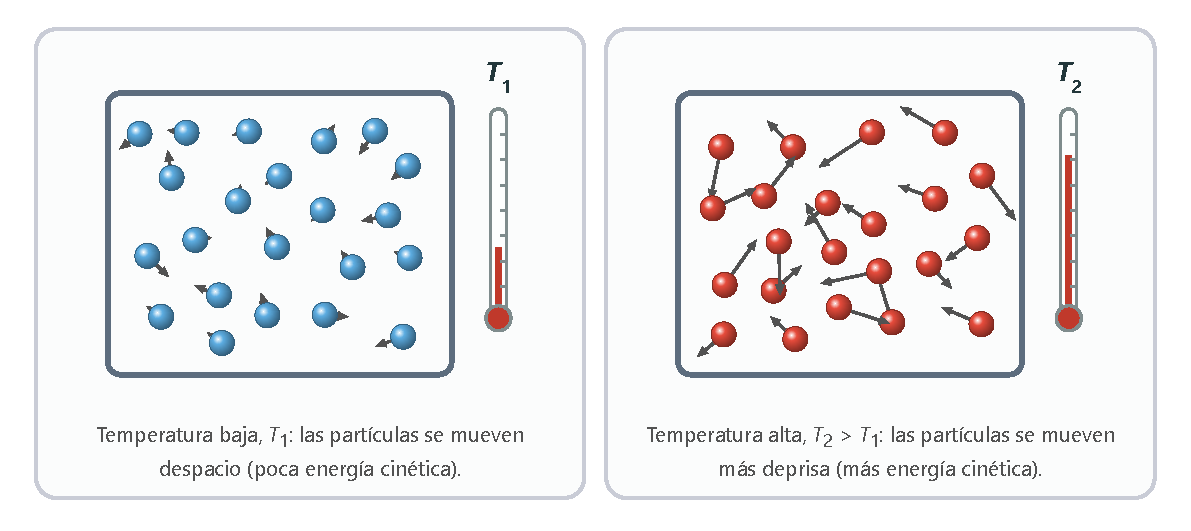
\includegraphics[width=0.9\textwidth]{images/UD12/particulas_temperatura}
    \caption{Al aumentar la temperatura, las partículas se mueven con más velocidad: su energía cinética media es mayor.}
    \label{fig:particulas_temperatura}
\end{figure}

\begin{definition}[Energía térmica y temperatura]
    La \textbf{energía térmica} de un cuerpo está relacionada con la energía cinética de sus partículas. La \textbf{temperatura} es una medida de la \textbf{energía cinética media} de esas partículas.
\end{definition}

Fíjate en la diferencia: un iceberg está más frío que una taza de café, pero, como tiene muchísimas más partículas, su energía térmica total es mucho mayor.

\subsection{Escalas de temperatura}

En la vida diaria medimos la temperatura en grados Celsius (\unit{\degreeCelsius}), pero la unidad del SI es el \textbf{kelvin} (\unit{\kelvin}). La escala Kelvin empieza en el \textbf{cero absoluto} (\qty{-273}{\degreeCelsius}), la temperatura más baja posible, a la que las partículas tendrían la mínima energía. Un kelvin y un grado Celsius tienen el mismo tamaño, así que:
\[ T\,(\unit{\kelvin}) = t\,(\unit{\degreeCelsius}) + 273 \]
Por eso una \textbf{variación} de temperatura vale lo mismo en las dos escalas: si el agua pasa de \qty{20}{\degreeCelsius} a \qty{30}{\degreeCelsius}, ha aumentado \qty{10}{\degreeCelsius} o, lo que es igual, \qty{10}{\kelvin}.

\subsection{¿Qué sucede cuando se ponen en contacto dos cuerpos a diferente temperatura? El equilibrio térmico}

La experiencia nos dice que, si ponemos en contacto dos cuerpos a distinta temperatura, al cabo de un tiempo los dos acaban a la misma temperatura: el café se enfría, el agua del vaso se calienta con la mano\ldots{} Las partículas del cuerpo caliente, al chocar con las del frío, les transfieren parte de su energía cinética (figura~\ref{fig:equilibrio_termico}).

\begin{figure}[H]
    \centering
    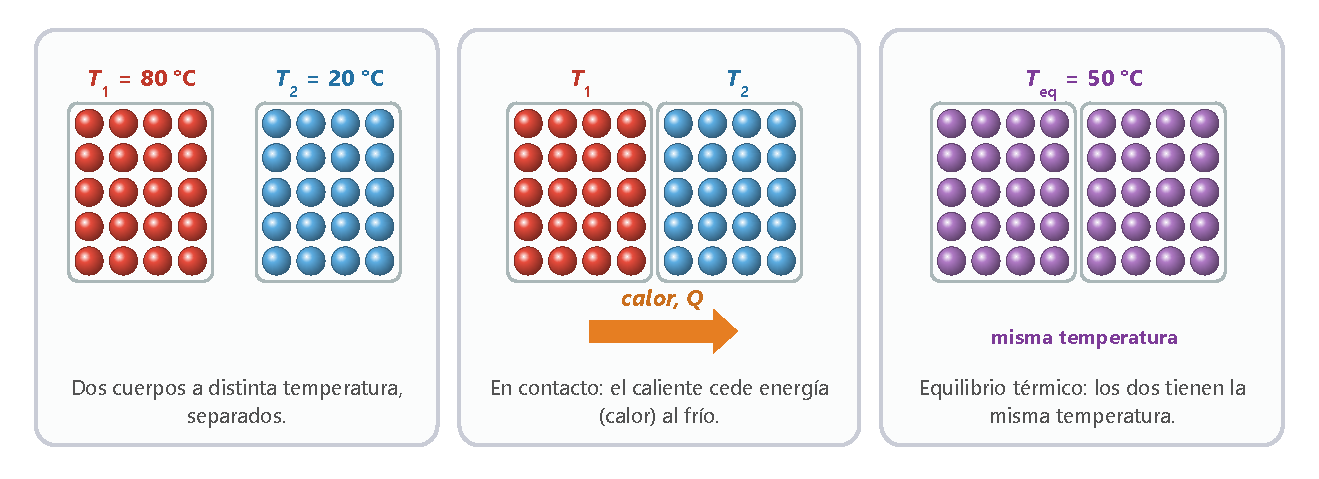
\includegraphics[width=\textwidth]{images/UD12/equilibrio_termico}
    \caption{Dos cuerpos en contacto intercambian energía hasta alcanzar el equilibrio térmico.}
    \label{fig:equilibrio_termico}
\end{figure}

\begin{definition}[Equilibrio térmico y calor]
    \begin{itemize}
        \item Dos cuerpos en contacto que están a la misma temperatura están en \textbf{equilibrio térmico}: ya no intercambian energía.
        \item El \textbf{calor} (\(Q\)) es la energía que se transfiere de un cuerpo a otro debido a su diferencia de temperatura. Pasa siempre, de forma espontánea, \textbf{del cuerpo de mayor temperatura al de menor temperatura}.
    \end{itemize}
\end{definition}

\begin{exercise}
    Razona si son verdaderas o falsas estas afirmaciones:
    \begin{enumerate}[label=\alph*)]
        \item Cuando baja la temperatura, las partículas de la materia se mueven más deprisa.
        \item Si dos cuerpos están a la misma temperatura, la energía cinética media de sus partículas es la misma.
        \item La energía térmica está relacionada con la energía cinética de las partículas del cuerpo.
        \item La energía, el calor y la temperatura se miden en las mismas unidades.
        \item La energía que pasa de un cuerpo a otro de menor temperatura se llama trabajo.
    \end{enumerate}
    \begin{solu}
        a) \textcolor{red}{Falso}: si baja la temperatura, las partículas se mueven más despacio. b) \textcolor{red}{Verdadero}: la temperatura mide la energía cinética media de las partículas. c) \textcolor{red}{Verdadero}. d) \textcolor{red}{Falso}: la energía y el calor se miden en julios, pero la temperatura se mide en \unit{\degreeCelsius} o en \unit{\kelvin}. e) \textcolor{red}{Falso}: se llama calor.
    \end{solu}
\end{exercise}

\begin{exercise}
    Expresa en kelvin estas temperaturas: \qty{25}{\degreeCelsius}, \qty{-18}{\degreeCelsius} y \qty{100}{\degreeCelsius}. Expresa en grados Celsius \qty{0}{\kelvin} y \qty{310}{\kelvin}.
    \begin{solu}
        \(T = t + 273\): \qty{25}{\degreeCelsius} \(\rightarrow\) \textcolor{red}{\qty{298}{\kelvin}}; \qty{-18}{\degreeCelsius} \(\rightarrow\) \textcolor{red}{\qty{255}{\kelvin}}; \qty{100}{\degreeCelsius} \(\rightarrow\) \textcolor{red}{\qty{373}{\kelvin}}. \(t = T - 273\): \qty{0}{\kelvin} \(\rightarrow\) \textcolor{red}{\qty{-273}{\degreeCelsius}}; \qty{310}{\kelvin} \(\rightarrow\) \textcolor{red}{\qty{37}{\degreeCelsius}} (la temperatura del cuerpo humano).
    \end{solu}
\end{exercise}

\subsection*{Actividades de consolidación: el calor}

\begin{exercise}
    Razona si estas afirmaciones son verdaderas o falsas:
    \begin{enumerate}[label=\alph*)]
        \item Entre dos cuerpos en equilibrio térmico no se transfiere calor.
        \item El calor pasa de un cuerpo a otro que está a mayor temperatura.
        \item Dos cuerpos en equilibrio térmico pueden estar a distinta temperatura.
        \item La energía es la forma de intercambiar trabajo y calor.
    \end{enumerate}
    \begin{solu}
        a) \textcolor{red}{Verdadero}. b) \textcolor{red}{Falso}: pasa del cuerpo de mayor temperatura al de menor temperatura. c) \textcolor{red}{Falso}: si están en equilibrio térmico, tienen la misma temperatura. d) \textcolor{red}{Falso}: es al revés; el trabajo y el calor son las formas de intercambiar energía.
    \end{solu}
\end{exercise}

\begin{exercise}
    Ponemos en contacto dos cuerpos a distinta temperatura.
    \begin{enumerate}[label=\alph*)]
        \item ¿Cuándo diremos que han alcanzado el equilibrio térmico?
        \item ¿Qué hay que hacer para que lo alcancen?
        \item ¿Cuál de los dos cede calor al otro?
    \end{enumerate}
    \begin{solu}
        a) Cuando los dos tengan la \textcolor{red}{misma temperatura}. b) Basta con \textcolor{red}{mantenerlos en contacto el tiempo suficiente}. c) El que está a \textcolor{red}{mayor temperatura} cede calor al que está a menor temperatura.
    \end{solu}
\end{exercise}

\begin{exercise}
    ¿En qué sentido se transfiere el calor entre dos cuerpos a diferente temperatura hasta que se alcanza el equilibrio térmico? ¿Puede ocurrir espontáneamente al revés?
    \begin{solu}
        Se transfiere \textcolor{red}{desde el cuerpo de mayor temperatura hacia el de menor temperatura}. \textcolor{red}{No} puede ocurrir al revés de forma espontánea: para sacar calor de un cuerpo frío y llevarlo a uno caliente (como hace un frigorífico) hay que aportar trabajo.
    \end{solu}
\end{exercise}

\begin{exercise}
    En 1798, Benjamin Thompson (conde de Rumford) dirigía la fabricación de cañones en el arsenal de Múnich. Le sorprendió lo mucho que se calentaban, en muy poco tiempo, las piezas de latón al taladrarlas, y todavía más las virutas que saltaban. Tanto, que con ese calor llegó a hacer hervir agua.
    \begin{enumerate}[label=\alph*)]
        \item ¿Qué transformación de energía observó Thompson?
        \item Busca información sobre Thompson y sobre la teoría del calor que se aceptaba en su época (el «calórico»). ¿Por qué fue importante su observación?
    \end{enumerate}
    \begin{solu}
        a) La transformación de \textcolor{red}{energía mecánica} (el trabajo del taladro contra el rozamiento) \textcolor{red}{en energía térmica}.
        b) Respuesta libre. Thompson nació en Norteamérica, luchó en el bando británico en la guerra de independencia de EE.~UU. y después trabajó para el gobierno de Baviera, donde reorganizó el ejército. En su época se pensaba que el calor era un fluido invisible, el \emph{calórico}, que pasaba de unos cuerpos a otros. Thompson se dio cuenta de que el taladro podía producir calor \textcolor{red}{sin límite} mientras siguiera trabajando, algo imposible si el calor fuera una sustancia almacenada en el metal. Su observación apuntaba a que \textcolor{red}{el calor está relacionado con el movimiento}, idea que Joule confirmó medio siglo después.
    \end{solu}
\end{exercise}

\begin{exercise}
    Explica la diferencia entre temperatura, energía térmica y calor usando este ejemplo: una piscina a \qty{25}{\degreeCelsius} y una taza de café a \qty{70}{\degreeCelsius}.
    \begin{solu}
        La \textcolor{red}{temperatura} del café es mayor: sus partículas tienen más energía cinética media. Sin embargo, la piscina tiene \textcolor{red}{más energía térmica}, porque tiene muchísimas más partículas. Si echamos el café en la piscina, se transferirá \textcolor{red}{calor} del café (mayor temperatura) al agua de la piscina, aunque esta tenga más energía térmica.
    \end{solu}
\end{exercise}

%========================================================================================
\section{Cantidad de calor y variación de temperatura}
%========================================================================================

¿Qué relación hay entre el calor que recibe un cuerpo y lo que sube su temperatura? Hagamos dos experiencias con un mismo hornillo, calentando siempre durante el mismo tiempo, de modo que todos los recipientes reciben la misma energía (figura~\ref{fig:calentamiento_experiencias}):
\begin{enumerate}[label=\numberballblue]
    \item Calentamos dos vasos con distinta cantidad de agua (\qty{400}{\gram} y \qty{200}{\gram}), inicialmente a la misma temperatura. El vaso con menos agua acaba más caliente.
    \item Calentamos la misma masa (\qty{400}{\gram}) de agua y de glicerina. La glicerina se calienta más que el agua.
\end{enumerate}

\begin{figure}[H]
    \centering
    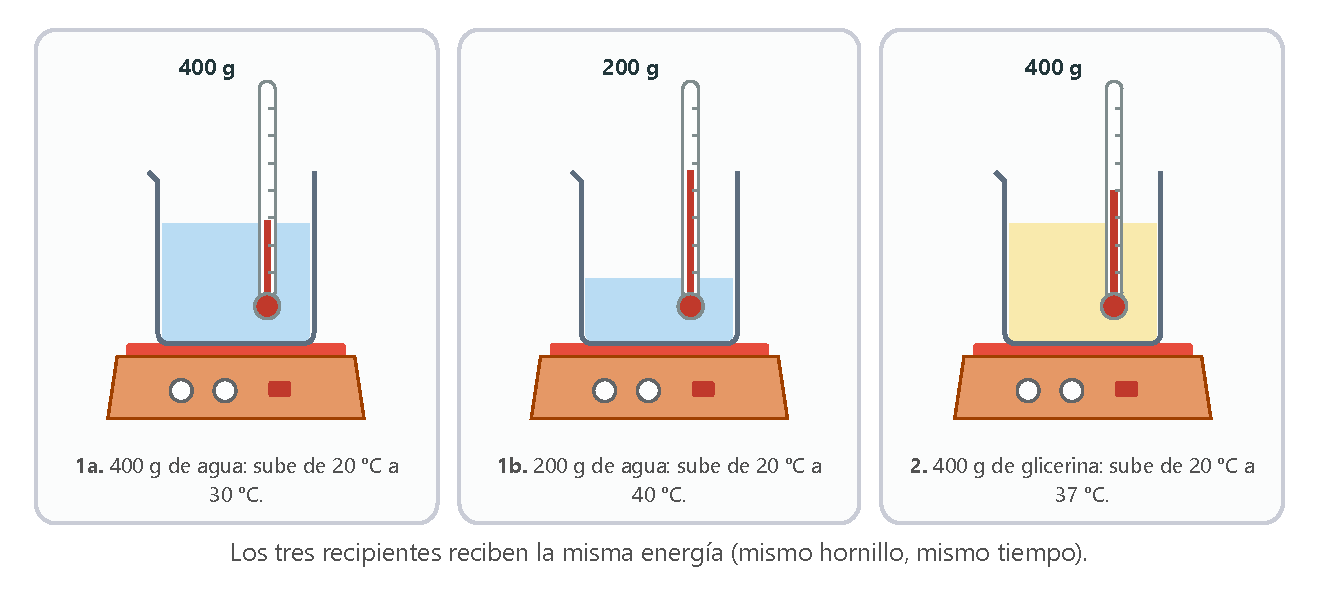
\includegraphics[width=\textwidth]{images/UD12/calentamiento_experiencias}
    \caption{Con la misma energía, la variación de temperatura depende de la masa y de la sustancia.}
    \label{fig:calentamiento_experiencias}
\end{figure}

De estas experiencias se deduce que:
\begin{itemize}
    \item La variación de temperatura depende de la \textbf{masa} del cuerpo: con la misma energía, cuanto más masa, menos sube la temperatura.
    \item La variación de temperatura depende de la \textbf{sustancia}.
    \item La energía transferida es \textbf{proporcional a la variación de temperatura}.
\end{itemize}

Todo ello se resume en una sola expresión:
\begin{equation*}
    \boxed{Q = m \cdot c \cdot (T_2 - T_1) = m \cdot c \cdot \Delta T}
\end{equation*}
donde \(Q\) es el calor transferido (\unit{\joule}); \(m\), la masa (\unit{\kg}); \(T_1\) y \(T_2\), las temperaturas inicial y final (\unit{\degreeCelsius} o \unit{\kelvin}), y \(c\), la \textbf{capacidad calorífica específica} o \textbf{calor específico} de la sustancia. Si el cuerpo se calienta, \(T_2 > T_1\) y \(Q\) es positivo (el cuerpo \emph{absorbe} calor); si se enfría, \(Q\) es negativo (el cuerpo \emph{cede} calor).

\begin{definition}[Capacidad calorífica específica]
    La \textbf{capacidad calorífica específica} (o calor específico), \(c\), de una sustancia es la energía que hay que transferir a \qty{1}{\kg} de esa sustancia para que su temperatura aumente \qty{1}{\degreeCelsius}. Se mide en \unit{\cunit} o, lo que es lo mismo, en \unit{\joule\per\kg\per\kelvin}.
\end{definition}

\begin{center}
    % --- tabla antigua ---
    % \begin{tblr}{colspec={lr}, hlines, vlines, row{1}={bg=ocre!85, fg=white, font=\bfseries}, column{2}={font=\small}}
        % Sustancia & \(c\) (\unit{\cunit}) \\
        % Aluminio & 910 \\
        % Cobre & 386 \\
        % Hierro & 447 \\
        % Plomo & 130 \\
        % Mercurio & 140 \\
        % Oxígeno & 920 \\
        % Agua líquida & 4180 \\
        % Hielo & 2100 \\
        % Glicerina & 2430 \\
    % \end{tblr}
    % --- tabla nueva ---
    {\small
    \begin{tabular}{@{}lr@{}}
        \toprule
        \textbf{Sustancia} & \textbf{\(c\) (\unit{\cunit})} \\
        \midrule
        Aluminio & 910 \\[3pt]
        Cobre & 386 \\[3pt]
        Hierro & 447 \\[3pt]
        Plomo & 130 \\[3pt]
        Mercurio & 140 \\[3pt]
        Oxígeno & 920 \\[3pt]
        Agua líquida & 4180 \\[3pt]
        Hielo & 2100 \\[3pt]
        Glicerina & 2430 \\
        \bottomrule
    \end{tabular}
    }
\end{center}

\begin{remark}
    El agua tiene una capacidad calorífica específica muy alta: hacen falta \qty{4180}{\joule} para que \qty{1}{\kg} de agua líquida suba \qty{1}{\degreeCelsius}. Por eso tarda mucho en calentarse y en enfriarse, y por eso los mares suavizan el clima de las zonas costeras: en verano se calientan menos que la tierra y en invierno se enfrían menos.
\end{remark}

En algunos textos antiguos y en la información nutricional se usa todavía la \textbf{caloría} (\unit{\calorie}), que es el calor necesario para que \qty{1}{\gram} de agua suba \qty{1}{\degreeCelsius}: \(\qty{1}{\calorie} = \qty{4.18}{\joule}\). Las «calorías» de los alimentos son en realidad kilocalorías (\qty{1}{\kilo\calorie} = \qty{4180}{\joule}).

\begin{example}
    Calcula la energía térmica que hay que comunicar a \qty{400}{\gram} de plomo para que su temperatura pase de \qty{15}{\degreeCelsius} a \qty{75}{\degreeCelsius}. Dato: \(c_{\text{Pb}} = \qty{130}{\cunit}\).
    \[ Q = m \cdot c_{\text{Pb}} \cdot (T_2 - T_1) = \num{0.400} \cdot 130 \cdot (75 - 15) = \textcolor{red}{\qty{3120}{\joule}} \]
\end{example}

\begin{exercise}
    Comprueba que la ecuación \(Q = m \cdot c \cdot (T_2 - T_1)\) es homogénea, es decir, que sus dos miembros tienen las mismas dimensiones. (Usa \(\Theta\) para la dimensión de la temperatura.)
    \begin{solu}
        El calor es una energía: \([Q] = \mathrm{M \cdot L^2 \cdot T^{-2}}\). Como \(c = \dfrac{Q}{m \cdot \Delta T}\), sus dimensiones son \([c] = \mathrm{L^2 \cdot T^{-2}} \cdot \Theta^{-1}\). Entonces:
        \[ [m] \cdot [c] \cdot [\Delta T] = \mathrm{M} \cdot \mathrm{L^2 \cdot T^{-2}} \cdot \Theta^{-1} \cdot \Theta = \textcolor{red}{\mathrm{M \cdot L^2 \cdot T^{-2}}} \]
        Los dos miembros tienen las dimensiones de una energía: la ecuación es \textcolor{red}{homogénea}.
    \end{solu}
\end{exercise}

\begin{exercise}
    ¿Qué energía térmica hay que comunicar a \qty{300}{\gram} de aluminio para calentarlos de \qty{20}{\degreeCelsius} a \qty{70}{\degreeCelsius}? Dato: \(c_{\text{Al}} = \qty{910}{\cunit}\).
    \begin{solu}
        \(Q = m \cdot c \cdot \Delta T = \num{0.300} \cdot 910 \cdot (70 - 20) = \textcolor{red}{\qty{13650}{\joule}}\).
    \end{solu}
\end{exercise}

\subsection{¿Cómo se utiliza un calorímetro?}

Un \textbf{calorímetro} es un recipiente construido para que la energía térmica apenas pueda entrar ni salir a través de sus paredes. Tiene paredes dobles, separadas por una cámara aislante, y una tapa con orificios por los que se introducen un \textbf{termómetro} y un \textbf{agitador} (figura~\ref{fig:calorimetro}). Se usa para aislar las sustancias del ambiente y estudiar los intercambios de energía que se producen entre ellas.

\begin{figure}[H]
    \centering
    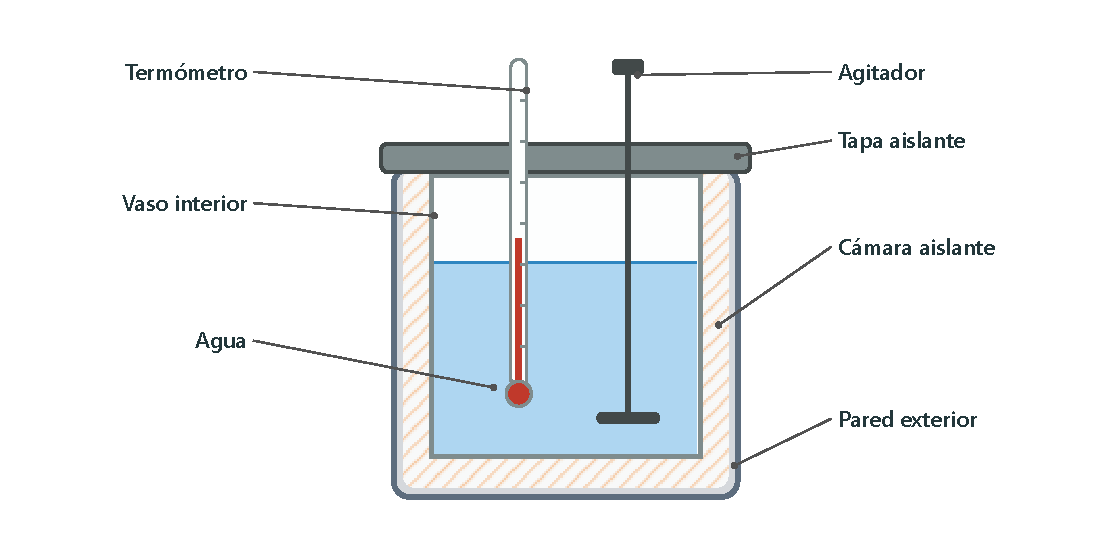
\includegraphics[width=0.8\textwidth]{images/UD12/calorimetro}
    \caption{Esquema de un calorímetro.}
    \label{fig:calorimetro}
\end{figure}

Supongamos que en un calorímetro con una masa \(m_2\) de agua a la temperatura \(T_2\) introducimos un cuerpo de masa \(m_1\) a mayor temperatura, \(T_1\). Al poco tiempo, todo alcanza el equilibrio térmico a la temperatura \(T_{\text{eq}}\), que está entre \(T_2\) y \(T_1\) (figura~\ref{fig:balance_calorimetro}).

\begin{figure}[H]
    \centering
    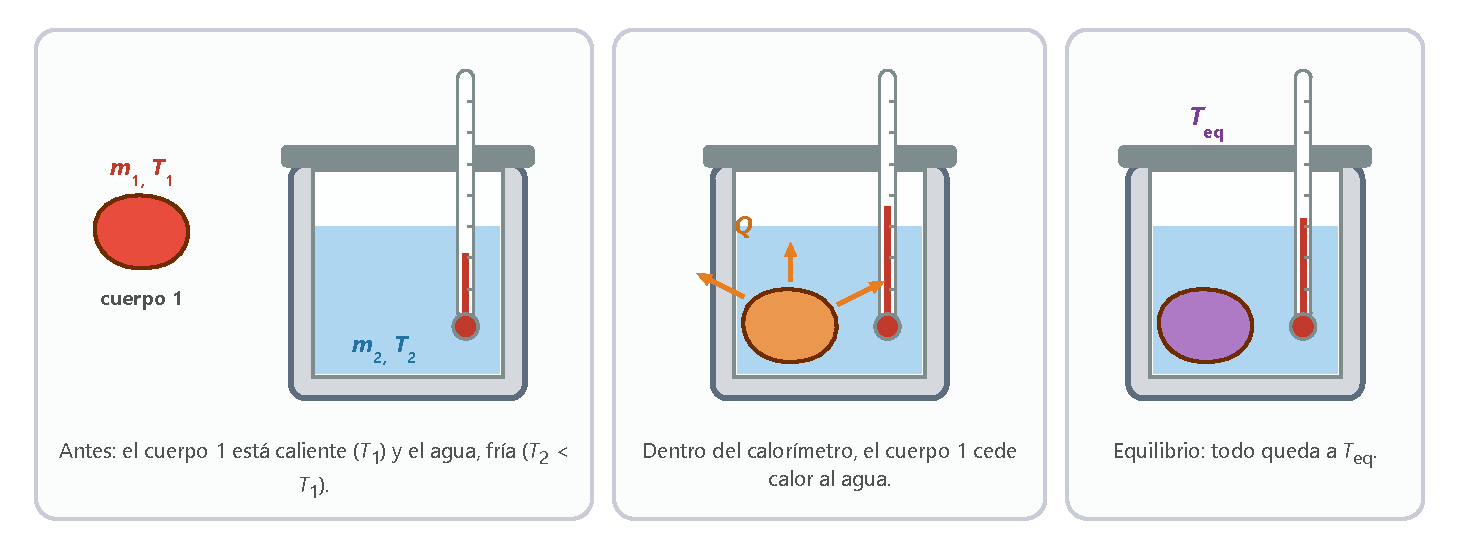
\includegraphics[width=\textwidth]{images/UD12/balance_calorimetro}
    \caption{El cuerpo caliente cede energía al agua hasta que ambos alcanzan el equilibrio térmico.}
    \label{fig:balance_calorimetro}
\end{figure}

\begin{itemize}
    \item Energía cedida por el cuerpo 1, que se enfría: \(Q_1 = m_1 \cdot c_1 \cdot (T_1 - T_{\text{eq}})\).
    \item Energía absorbida por el agua, que se calienta: \(Q_2 = m_2 \cdot c_2 \cdot (T_{\text{eq}} - T_2)\).
\end{itemize}

Como no se escapa energía del calorímetro, toda la energía que cede uno la absorbe el otro:

\begin{definition}[Balance de energía en un calorímetro]
    \[ \text{energía cedida por el cuerpo caliente} = \text{energía absorbida por el cuerpo frío} \]
    \[ \boxed{m_1 \cdot c_1 \cdot (T_1 - T_{\text{eq}}) = m_2 \cdot c_2 \cdot (T_{\text{eq}} - T_2)} \]
\end{definition}

\begin{example}
    Se mezclan \qty{0.6}{\kg} de agua a \qty{80}{\degreeCelsius} con \qty{0.9}{\kg} de agua a \qty{20}{\degreeCelsius}. ¿Qué temperatura tendrá la mezcla en el equilibrio térmico? Dato: \(c_{\text{agua}} = \qty{4180}{\cunit}\).

    El agua caliente cede energía y la fría la absorbe:
    \[ Q_{\text{cedido}} = \num{0.6} \cdot 4180 \cdot (80 - T_{\text{eq}}) \qquad Q_{\text{absorbido}} = \num{0.9} \cdot 4180 \cdot (T_{\text{eq}} - 20) \]
    Igualamos ambas energías; el factor \(c_{\text{agua}}\) aparece en los dos miembros y se simplifica:
    \[ \num{0.6} \cdot (80 - T_{\text{eq}}) = \num{0.9} \cdot (T_{\text{eq}} - 20) \Rightarrow 48 - \num{0.6}\,T_{\text{eq}} = \num{0.9}\,T_{\text{eq}} - 18 \]
    \[ 66 = \num{1.5}\,T_{\text{eq}} \Rightarrow T_{\text{eq}} = \frac{66}{\num{1.5}} = \textcolor{red}{\qty{44}{\degreeCelsius}} \]
    La temperatura queda más cerca de la del agua fría, porque hay más cantidad de ella.
\end{example}

\begin{exercise}
    Se mezclan \qty{3}{\liter} de agua a \qty{20}{\degreeCelsius} con \qty{1}{\liter} de agua a \qty{100}{\degreeCelsius}. ¿Cuál será la temperatura de la mezcla en el equilibrio térmico? (Un litro de agua tiene una masa de \qty{1}{\kg}.)
    \begin{solu}
        \textcolor{blue}{Balance: \(m_1 \cdot c \cdot (T_1 - T_{\text{eq}}) = m_2 \cdot c \cdot (T_{\text{eq}} - T_2)\); como es la misma sustancia, \(c\) se simplifica:}
        \[ 1 \cdot (100 - T_{\text{eq}}) = 3 \cdot (T_{\text{eq}} - 20) \Rightarrow 160 = 4\,T_{\text{eq}} \Rightarrow T_{\text{eq}} = \textcolor{red}{\qty{40}{\degreeCelsius}} \]
    \end{solu}
\end{exercise}

\begin{exercise}
    Queremos enfriar \qty{3}{\kg} de agua a \qty{60}{\degreeCelsius} añadiendo agua a \qty{15}{\degreeCelsius}. ¿Cuánta agua fría hay que añadir para que la mezcla quede a \qty{30}{\degreeCelsius}?
    \begin{solu}
        \textcolor{blue}{Energía cedida por el agua caliente:} \(Q = 3 \cdot 4180 \cdot (60 - 30) = \qty{376200}{\joule}\).

        \textcolor{blue}{La absorbe el agua fría:} \(\num{376200} = m \cdot 4180 \cdot (30 - 15) \Rightarrow m = \dfrac{\num{376200}}{\num{62700}} = \textcolor{red}{\qty{6}{\kg}}\) de agua (6 litros).
    \end{solu}
\end{exercise}

\subsection{Determinación de la capacidad calorífica específica}

Para medir el calor específico de un sólido, lo calentamos hasta una temperatura conocida y lo introducimos en un calorímetro con agua. Midiendo las masas y las temperaturas, el balance de energía nos permite despejar la única incógnita, \(c\):
\[ \text{energía cedida por el sólido} = \text{energía absorbida por el agua} \]

\begin{example}
    Un calorímetro contiene \qty{0.500}{\kg} de agua a \qty{20.0}{\degreeCelsius}. Se introduce un bloque de plomo de \qty{0.200}{\kg} a \qty{95.0}{\degreeCelsius} y, en el equilibrio térmico, el termómetro marca \qty{20.9}{\degreeCelsius}. Calcula la capacidad calorífica específica del plomo.

    Energía absorbida por el agua, que sube \qty{0.9}{\degreeCelsius}:
    \[ Q = m_{\text{agua}} \cdot c_{\text{agua}} \cdot (T_{\text{eq}} - T_{\text{agua}}) = \num{0.500} \cdot 4180 \cdot (\num{20.9} - \num{20.0}) = \qty{1881}{\joule} \]
    Energía cedida por el plomo, que baja de \qty{95.0}{\degreeCelsius} a \qty{20.9}{\degreeCelsius}:
    \[ Q = m_{\text{Pb}} \cdot c_{\text{Pb}} \cdot (T_{\text{Pb}} - T_{\text{eq}}) = \num{0.200} \cdot c_{\text{Pb}} \cdot \num{74.1} = \num{14.82} \cdot c_{\text{Pb}} \]
    Igualamos ambas energías y despejamos:
    \[ c_{\text{Pb}} = \frac{1881}{\num{14.82}} = \textcolor{red}{\qty{127}{\cunit}} \]
    El valor de la tabla es \qty{130}{\cunit}. La pequeña diferencia se debe a los errores de medida (el termómetro aprecia décimas) y a que una parte de la energía se emplea en calentar el propio calorímetro o se pierde al trasladar el bloque.
\end{example}

\begin{exercise}
    En un calorímetro con \qty{1.5}{\liter} de agua a \qty{18}{\degreeCelsius} se introducen \qty{250}{\gram} de un metal a \qty{200}{\degreeCelsius}. Si la temperatura de equilibrio es \qty{24.4}{\degreeCelsius}, ¿cuál es el calor específico del metal? ¿De qué metal puede tratarse?
    \begin{solu}
        \textcolor{blue}{Energía absorbida por el agua:} \(Q = \num{1.5} \cdot 4180 \cdot (\num{24.4} - 18) = \qty{40128}{\joule}\).

        \textcolor{blue}{Energía cedida por el metal:} \(Q = \num{0.250} \cdot c \cdot (200 - \num{24.4}) = \num{43.9} \cdot c\).

        \(c = \dfrac{\num{40128}}{\num{43.9}} \approx \textcolor{red}{\qty{914}{\cunit}}\). Según la tabla, probablemente es \textcolor{red}{aluminio} (\qty{910}{\cunit}).
    \end{solu}
\end{exercise}

\begin{exercise}
    Se introducen \qty{400}{\gram} de una sustancia a \qty{80}{\degreeCelsius} en un calorímetro con \qty{1.5}{\kg} de agua a \qty{15}{\degreeCelsius}. En el equilibrio, el termómetro marca \qty{19}{\degreeCelsius}. Calcula la capacidad calorífica específica de la sustancia.
    \begin{solu}
        \textcolor{blue}{La sustancia se enfría de \qty{80}{\degreeCelsius} a \qty{19}{\degreeCelsius} y el agua se calienta de \qty{15}{\degreeCelsius} a \qty{19}{\degreeCelsius}:}
        \[ \num{0.4} \cdot c \cdot (80 - 19) = \num{1.5} \cdot 4180 \cdot (19 - 15) \Rightarrow \num{24.4} \cdot c = \num{25080} \]
        \[ c = \textcolor{red}{\qty{1028}{\cunit}} \]
    \end{solu}
\end{exercise}

\begin{exercise}
    Un calorímetro contiene \qty{600}{\gram} de agua a \qty{22}{\degreeCelsius}. Se introduce un bloque de cobre de \qty{200}{\gram} a \qty{90}{\degreeCelsius}. Calcula la temperatura de equilibrio. Dato: \(c_{\text{Cu}} = \qty{386}{\cunit}\).
    \begin{solu}
        \textcolor{blue}{Energía absorbida por el agua:} \(\num{0.600} \cdot 4180 \cdot (T_{\text{eq}} - 22) = 2508\,T_{\text{eq}} - \num{55176}\).

        \textcolor{blue}{Energía cedida por el cobre:} \(\num{0.200} \cdot 386 \cdot (90 - T_{\text{eq}}) = 6948 - \num{77.2}\,T_{\text{eq}}\).

        \textcolor{blue}{Igualamos:} \(\num{2585.2}\,T_{\text{eq}} = \num{62124} \Rightarrow T_{\text{eq}} = \textcolor{red}{\qty{24.0}{\degreeCelsius}}\).
    \end{solu}
\end{exercise}

\subsection*{Actividades de consolidación: cantidad de calor y variación de temperatura}

\begin{exercise}
    Copia y completa en tu cuaderno: «La capacidad calorífica específica del hierro es \qty{447}{\cunit}; esto significa que, para que \qty{1}{\kg} de hierro aumente su temperatura \qty{1}{\degreeCelsius}, hay que transferirle \ldots{} J».
    \begin{solu}
        \ldots{} hay que transferirle \textcolor{red}{\qty{447}{\joule}}.
    \end{solu}
\end{exercise}

\begin{exercise}
    ¿Qué energía térmica hay que comunicar a \qty{750}{\gram} de aluminio para elevar su temperatura de \qty{15}{\degreeCelsius} a \qty{75}{\degreeCelsius}? Dato: \(c_{\text{Al}} = \qty{910}{\cunit}\).
    \begin{solu}
        \(Q = \num{0.750} \cdot 910 \cdot (75 - 15) = \textcolor{red}{\qty{40950}{\joule}}\).
    \end{solu}
\end{exercise}

\begin{exercise}
    Se mezclan \qty{0.6}{\kg} de agua a \qty{75}{\degreeCelsius} con \qty{0.4}{\kg} de agua a \qty{25}{\degreeCelsius}. ¿Cuál será la temperatura de la mezcla en el equilibrio térmico?
    \begin{solu}
        \(\num{0.6} \cdot (75 - T_{\text{eq}}) = \num{0.4} \cdot (T_{\text{eq}} - 25) \Rightarrow 45 + 10 = T_{\text{eq}} \Rightarrow T_{\text{eq}} = \textcolor{red}{\qty{55}{\degreeCelsius}}\).
    \end{solu}
\end{exercise}

\begin{exercise}
    ¿Qué energía térmica se necesita para calentar \qty{250}{\gram} de agua desde \qty{10}{\degreeCelsius} hasta \qty{60}{\degreeCelsius}?
    \begin{solu}
        \(Q = \num{0.250} \cdot 4180 \cdot 50 = \textcolor{red}{\qty{52250}{\joule}}\).
    \end{solu}
\end{exercise}

\begin{exercise}
    ¿Qué energía se necesita para elevar \qty{25}{\degreeCelsius} la temperatura de \qty{300}{\gram} de cobre? Dato: \(c_{\text{Cu}} = \qty{386}{\cunit}\).
    \begin{solu}
        \(Q = \num{0.300} \cdot 386 \cdot 25 = \textcolor{red}{\qty{2895}{\joule}}\).
    \end{solu}
\end{exercise}

\begin{exercise}
    ¿Cuánto aumenta la temperatura de \qty{1}{\kg} de cobre si le comunicamos \qty{772}{\joule}?
    \begin{solu}
        \(\Delta T = \dfrac{Q}{m \cdot c} = \dfrac{772}{1 \cdot 386} = \textcolor{red}{\qty{2}{\degreeCelsius}}\).
    \end{solu}
\end{exercise}

\begin{exercise}
    ¿Qué energía térmica hay que transferir a \qty{3}{\kg} de plomo para que su temperatura suba \qty{20}{\degreeCelsius}? Dato: \(c_{\text{Pb}} = \qty{130}{\cunit}\).
    \begin{solu}
        \(Q = 3 \cdot 130 \cdot 20 = \textcolor{red}{\qty{7800}{\joule}}\).
    \end{solu}
\end{exercise}

\begin{exercise}
    ¿Qué energía se necesita para calentar una barra de hierro de \qty{800}{\gram} desde \qty{20}{\degreeCelsius} hasta \qty{120}{\degreeCelsius}? Dato: \(c_{\text{Fe}} = \qty{447}{\cunit}\).
    \begin{solu}
        \(Q = \num{0.800} \cdot 447 \cdot (120 - 20) = \textcolor{red}{\qty{35760}{\joule}}\).
    \end{solu}
\end{exercise}

\begin{exercise}
    Un cuerpo de \qty{4}{\kg} tiene una capacidad calorífica específica de \qty{394}{\cunit}. ¿Cuánta energía hay que suministrarle para calentarlo de \qty{10}{\degreeCelsius} a \qty{40}{\degreeCelsius}? ¿Y si fuera de agua?
    \begin{solu}
        \(Q = 4 \cdot 394 \cdot 30 = \textcolor{red}{\qty{47280}{\joule}}\). Si fuera agua: \(Q = 4 \cdot 4180 \cdot 30 = \textcolor{red}{\qty{501600}{\joule}}\), más de diez veces más.
    \end{solu}
\end{exercise}

\begin{exercise}
    Responde a estas preguntas:
    \begin{enumerate}[label=\alph*)]
        \item ¿Qué es la capacidad calorífica específica? ¿En qué unidades se mide?
        \item Busca dos sustancias, que no estén en la tabla de la unidad, con una capacidad calorífica específica alta.
        \item Busca dos sustancias, que no estén en la tabla, con una capacidad calorífica específica baja.
    \end{enumerate}
    \begin{solu}
        a) Es la energía que hay que transferir a \qty{1}{\kg} de una sustancia para que su temperatura suba \qty{1}{\degreeCelsius}. Se mide en \textcolor{red}{\unit{\cunit}} (o \unit{\joule\per\kg\per\kelvin}).
        b) Respuesta libre. Por ejemplo, el \textcolor{red}{etanol} (unos \qty{2440}{\cunit}), el \textcolor{red}{aceite de oliva} (unos \qty{2000}{\cunit}) o la \textcolor{red}{madera} (unos \qty{1700}{\cunit}).
        c) Respuesta libre. Los metales tienen calores específicos bajos: por ejemplo, la \textcolor{red}{plata} (unos \qty{235}{\cunit}) o el \textcolor{red}{oro} (unos \qty{129}{\cunit}).
    \end{solu}
\end{exercise}

\begin{exercise}
    Se necesitan \qty{2430}{\joule} para elevar \qty{1}{\degreeCelsius} la temperatura de \qty{1}{\kg} de una sustancia. ¿Cuál es su capacidad calorífica específica? ¿Qué sustancia de la tabla puede ser?
    \begin{solu}
        \(c = \textcolor{red}{\qty{2430}{\cunit}}\); según la tabla, se trata de la \textcolor{red}{glicerina}.
    \end{solu}
\end{exercise}

\begin{exercise}
    Un trozo de metal de \qty{80}{\gram} se calienta a \qty{180}{\degreeCelsius} y se introduce en un calorímetro con \qty{0.4}{\kg} de agua a \qty{18}{\degreeCelsius}. Si la temperatura final de equilibrio es \qty{21}{\degreeCelsius}, calcula la capacidad calorífica específica del metal.
    \begin{solu}
        \textcolor{blue}{Energía absorbida por el agua:} \(Q = \num{0.4} \cdot 4180 \cdot (21 - 18) = \qty{5016}{\joule}\).

        \textcolor{blue}{Energía cedida por el metal:} \(Q = \num{0.080} \cdot c \cdot (180 - 21) = \num{12.72} \cdot c\).

        \(c = \dfrac{5016}{\num{12.72}} = \textcolor{red}{\qty{394}{\cunit}}\) (un valor parecido al del cobre o al del latón).
    \end{solu}
\end{exercise}

\begin{exercise}
    Queremos medir la capacidad calorífica específica de una pieza de cobre con un calorímetro.
    \begin{enumerate}[label=\alph*)]
        \item ¿Para qué sirve un calorímetro?
        \item Dibuja un esquema de un calorímetro y señala sus partes.
        \item ¿Qué instrumento de medida lleva incorporado?
    \end{enumerate}
    \begin{solu}
        a) Sirve para \textcolor{red}{aislar del ambiente} las sustancias y estudiar los intercambios de energía térmica entre ellas, por ejemplo, para medir calores específicos.
        b) Como en la figura~\ref{fig:calorimetro}: \textcolor{red}{pared exterior, cámara aislante, vaso interior con el agua, tapa aislante, termómetro y agitador}.
        c) Un \textcolor{red}{termómetro}.
    \end{solu}
\end{exercise}

\begin{exercise}
    Se calientan \qty{400}{\gram} de cobre a \qty{100}{\degreeCelsius} y se introducen en un calorímetro con \qty{600}{\gram} de agua a \qty{16}{\degreeCelsius}. Al poco tiempo, el termómetro marca \qty{20.8}{\degreeCelsius}.
    \begin{enumerate}[label=\alph*)]
        \item Calcula con estos datos la capacidad calorífica específica del cobre.
        \item Compara el resultado con el de la tabla. ¿A qué puede deberse la diferencia?
    \end{enumerate}
    \begin{solu}
        a) \(\num{0.4} \cdot c_{\text{Cu}} \cdot (100 - \num{20.8}) = \num{0.6} \cdot 4180 \cdot (\num{20.8} - 16) \Rightarrow \num{31.68} \cdot c_{\text{Cu}} = \num{12038.4}\)
        \[ c_{\text{Cu}} = \textcolor{red}{\qty{380}{\cunit}} \]
        b) La tabla da \qty{386}{\cunit}. La diferencia se debe a las \textcolor{red}{pérdidas de energía} (parte del calor calienta el propio calorímetro o escapa al ambiente) y a los \textcolor{red}{errores de medida}.
    \end{solu}
\end{exercise}

\begin{exercise}
    Mezclamos \qty{600}{\gram} de una sustancia a \qty{20}{\degreeCelsius} con \qty{200}{\gram} de la misma sustancia a \qty{80}{\degreeCelsius}. ¿Cuál será la temperatura de la mezcla en el equilibrio térmico?
    \begin{solu}
        \(\num{0.6} \cdot c \cdot (T_{\text{eq}} - 20) = \num{0.2} \cdot c \cdot (80 - T_{\text{eq}}) \Rightarrow \num{0.8}\,T_{\text{eq}} = 28 \Rightarrow T_{\text{eq}} = \textcolor{red}{\qty{35}{\degreeCelsius}}\). No hace falta conocer \(c\), porque se simplifica.
    \end{solu}
\end{exercise}

\begin{exercise}
    Se mezclan \qty{3}{\liter} de agua a \qty{30}{\degreeCelsius} con \qty{2}{\liter} de agua a \qty{90}{\degreeCelsius}. ¿Qué temperatura alcanza la mezcla?
    \begin{solu}
        \(3 \cdot (T_{\text{eq}} - 30) = 2 \cdot (90 - T_{\text{eq}}) \Rightarrow 5\,T_{\text{eq}} = 270 \Rightarrow T_{\text{eq}} = \textcolor{red}{\qty{54}{\degreeCelsius}}\).
    \end{solu}
\end{exercise}

\begin{exercise}
    Un kilogramo de mercurio y un kilogramo de agua reciben la misma energía térmica. ¿Cuál de los dos se calienta más? ¿Por qué?
    \begin{solu}
        Se calienta más el \textcolor{red}{mercurio}, porque su capacidad calorífica específica (\qty{140}{\cunit}) es mucho menor que la del agua (\qty{4180}{\cunit}): con la misma energía, su temperatura sube unas 30 veces más.
    \end{solu}
\end{exercise}

\begin{exercise}
    Una pieza de hierro de \qty{200}{\gram} a \qty{90}{\degreeCelsius} se introduce en un termo con \qty{400}{\gram} de agua a \qty{18}{\degreeCelsius}. Describe lo que ocurre y calcula la temperatura final. Dato: \(c_{\text{Fe}} = \qty{447}{\cunit}\).
    \begin{solu}
        Se transfiere energía del cuerpo de mayor temperatura (el hierro) al de menor temperatura (el agua) hasta que ambos alcanzan la misma temperatura.
        \[ \num{0.2} \cdot 447 \cdot (90 - T_{\text{eq}}) = \num{0.4} \cdot 4180 \cdot (T_{\text{eq}} - 18) \]
        \[ 8046 - \num{89.4}\,T_{\text{eq}} = 1672\,T_{\text{eq}} - \num{30096} \Rightarrow T_{\text{eq}} = \frac{\num{38142}}{\num{1761.4}} = \textcolor{red}{\qty{21.7}{\degreeCelsius}} \]
    \end{solu}
\end{exercise}

\begin{exercise}
    Un hervidor eléctrico calienta \qty{4}{\liter} de agua de \qty{15}{\degreeCelsius} a \qty{85}{\degreeCelsius} en \qty{15}{\minute}. ¿Qué energía térmica proporciona cada minuto? ¿Cuál es su potencia útil?
    \begin{solu}
        \(Q = 4 \cdot 4180 \cdot (85 - 15) = \qty{1170400}{\joule}\). Cada minuto: \(\dfrac{\num{1170400}}{15} \approx \textcolor{red}{\qty{78000}{\joule}}\). Potencia útil: \(P = \dfrac{Q}{t} = \dfrac{\num{1170400}}{900} \approx \textcolor{red}{\qty{1300}{\watt}}\).
    \end{solu}
\end{exercise}

\begin{exercise}
    En un calorímetro se mezcla una masa \(m_1\) de plomo a la temperatura \(T_1\) con una masa \(m_2\) de agua a la temperatura \(T_2\), menor que \(T_1\). Al poco tiempo se alcanza el equilibrio a \(T_{\text{eq}}\). Indica cuáles de estas afirmaciones son falsas y corrígelas:
    \begin{enumerate}[label=\alph*)]
        \item La energía absorbida por el plomo es igual a la energía cedida por el agua.
        \item La temperatura de equilibrio es menor que la temperatura inicial del plomo.
        \item La temperatura de equilibrio es menor que la temperatura inicial del agua.
        \item \(m_1 \cdot c_{\text{Pb}} \cdot (T_1 - T_{\text{eq}}) = m_2 \cdot c_{\text{agua}} \cdot (T_{\text{eq}} - T_2)\).
        \item La energía que el plomo transfiere al agua hace que la temperatura de esta aumente.
    \end{enumerate}
    \begin{solu}
        Son falsas \textcolor{red}{a) y c)}. a) Es al revés: la energía \emph{cedida} por el plomo es igual a la \emph{absorbida} por el agua. c) La temperatura de equilibrio es \emph{mayor} que la temperatura inicial del agua (el agua se calienta). b), d) y e) son verdaderas.
    \end{solu}
\end{exercise}

%========================================================================================
\section[Calor en los cambios de estado]{Cantidad de calor transferida en los cambios de estado}
%========================================================================================

Hasta ahora, cuando un cuerpo recibía o cedía energía térmica, su temperatura cambiaba. Pero hay una excepción importante: \textbf{mientras una sustancia pura cambia de estado, su temperatura permanece constante}, aunque siga recibiendo (o cediendo) energía.

Podemos comprobarlo fundiendo naftalina. Ponemos unas bolitas de naftalina en un tubo de ensayo con un termómetro cuyo bulbo quede cubierto, introducimos el tubo en un vaso con agua y lo calentamos. Cada minuto anotamos la temperatura, mientras agitamos el agua, y representamos la temperatura frente al tiempo.

\subsection{Análisis de una gráfica de calentamiento}

\begin{center}
    \begin{tikzpicture}
        \begin{axis}[grafica, width=8cm, height=5.5cm, xlabel={\(t\) (min)}, ylabel={\(T\) (\unit{\degreeCelsius})}, xmin=0, xmax=13, ymin=72, ymax=86, xtick={0,2,...,12}, ytick={72,74,...,86}, title={\small Calentamiento de la naftalina}]
            \addplot[mark=none] coordinates {(0,74) (6,80) (10,80) (12,84)};
            \node[anchor=south, font=\footnotesize] at (axis cs:8,80.2) {fusión (sólido + líquido)};
            \node[anchor=west, font=\footnotesize] at (axis cs:2.2,75.4) {sólido};
            \node[anchor=east, font=\footnotesize] at (axis cs:10.6,83.6) {líquido};
        \end{axis}
    \end{tikzpicture}
\end{center}

En la gráfica se distinguen tres tramos:
\begin{enumerate}[label=\numberballblue]
    \item Un tramo ascendente: la naftalina sólida se calienta hasta \qty{80}{\degreeCelsius}, su \textbf{temperatura de fusión}.
    \item Un tramo \textbf{horizontal}: mientras se funde, la temperatura no cambia. Se mantiene constante \textbf{durante todo el cambio de estado}, hasta que toda la naftalina es líquida.
    \item Otro tramo ascendente: la naftalina líquida sigue calentándose.
\end{enumerate}

\subsection{El calor latente de cambio de estado}

¿En qué se emplea la energía que recibe la sustancia durante el cambio de estado, si no aumenta su temperatura? Se usa en \textbf{vencer las fuerzas de cohesión} que mantienen unidas las partículas en el sólido (en la fusión) o en el líquido (en la vaporización). La energía cinética media de las partículas no cambia, así que el termómetro no detecta nada; por eso decimos que es un calor «latente» (escondido).

\begin{definition}[Calor latente de cambio de estado]
    El \textbf{calor latente}, \(L\), de un cambio de estado es la energía que hay que transferir a \qty{1}{\kg} de una sustancia pura para que cambie de estado, a una presión determinada y a la temperatura del cambio de estado. Se mide en \unit{\joule\per\kg}. El calor necesario para que cambie de estado una masa \(m\) es:
    \[ \boxed{Q = m \cdot L} \]
\end{definition}

\subsection{Calor latente de fusión y de vaporización}

En la gráfica de calentamiento de una sustancia desde el estado sólido hasta el gaseoso aparecen dos tramos horizontales:
\begin{itemize}
    \item El primero corresponde a la \textbf{fusión} (paso de sólido a líquido). El calor necesario es \(Q = m \cdot L_f\), donde \(L_f\) es el \textbf{calor latente de fusión}. Es igual al calor latente de solidificación, pero en la fusión la sustancia \emph{absorbe} esa energía y en la solidificación la \emph{cede}.
    \item El segundo corresponde a la \textbf{vaporización} (paso de líquido a gas). El calor necesario es \(Q = m \cdot L_v\), donde \(L_v\) es el \textbf{calor latente de vaporización}, igual al de condensación: para vaporizar hay que aportar energía, y al condensarse el vapor la desprende.
\end{itemize}

\begin{center}
    % --- tabla antigua ---
    % \begin{tblr}{colspec={lcccc}, hlines, vlines, row{1}={bg=ocre!85, fg=white, font=\bfseries\small}, cells={font=\small}}
        % Sustancia & \(T_f\) (\unit{\degreeCelsius}) & \(L_f\) (\unit{\joule\per\kg}) & \(T_{eb}\) (\unit{\degreeCelsius}) & \(L_v\) (\unit{\joule\per\kg}) \\
        % Agua & 0 & \num{3.35e5} & 100 & \num{2.2e6} \\
        % Aluminio & 660 & \num{4.0e5} & 2470 & \num{1.05e7} \\
        % Cobre & 1085 & \num{2.05e5} & 2560 & \num{4.8e6} \\
        % Hierro & 1538 & \num{2.75e5} & 2860 & \num{6.3e6} \\
        % Plomo & 327 & \num{2.3e4} & 1750 & \num{8.6e5} \\
        % Mercurio & \num{-39} & \num{1.1e4} & 357 & \num{2.9e5} \\
    % \end{tblr}
    % --- tabla nueva ---
    {\small
    \begin{tabular}{@{}lcccc@{}}
        \toprule
        \textbf{Sustancia} & \textbf{\(T_f\) (\unit{\degreeCelsius})} & \textbf{\(L_f\) (\unit{\joule\per\kg})} & \textbf{\(T_{eb}\) (\unit{\degreeCelsius})} & \textbf{\(L_v\) (\unit{\joule\per\kg})} \\
        \midrule
        Agua & 0 & \num{3.35e5} & 100 & \num{2.2e6} \\[3pt]
        Aluminio & 660 & \num{4.0e5} & 2470 & \num{1.05e7} \\[3pt]
        Cobre & 1085 & \num{2.05e5} & 2560 & \num{4.8e6} \\[3pt]
        Hierro & 1538 & \num{2.75e5} & 2860 & \num{6.3e6} \\[3pt]
        Plomo & 327 & \num{2.3e4} & 1750 & \num{8.6e5} \\[3pt]
        Mercurio & \num{-39} & \num{1.1e4} & 357 & \num{2.9e5} \\
        \bottomrule
    \end{tabular}
    }
\end{center}

Observa que el calor latente de vaporización del agua es casi siete veces mayor que el de fusión: separar por completo las moléculas del líquido cuesta mucha más energía que deshacer la estructura del hielo.

\begin{example}
    Calcula la energía que hay que transferir a \qty{2}{\kg} de hielo a \qty{-10}{\degreeCelsius} para convertirlos en vapor de agua a \qty{100}{\degreeCelsius}. Datos: \(c_{\text{hielo}} = \qty{2100}{\cunit}\); \(c_{\text{agua}} = \qty{4180}{\cunit}\); \(L_f = \qty{3.35e5}{\joule\per\kg}\); \(L_v = \qty{2.2e6}{\joule\per\kg}\).

    \begin{center}
        \begin{tikzpicture}
            \begin{axis}[grafica, width=9cm, height=5.5cm, xlabel={\(t\)}, ylabel={\(T\) (\unit{\degreeCelsius})}, xmin=0, xmax=12, ymin=-20, ymax=120, xtick=\empty, ytick={-10,0,100}, title={\small Calentamiento del agua}]
                \addplot[mark=none] coordinates {(0,-10) (0.6,0) (2.2,0) (4.2,100) (10.2,100) (11,115)};
                \node[anchor=west, font=\scriptsize] at (axis cs:0.5,-12) {tramo 1: hielo};
                \node[anchor=south, font=\scriptsize] at (axis cs:1.4,2) {tramo 2};
                \node[anchor=west, font=\scriptsize] at (axis cs:3.3,45) {tramo 3: líquido};
                \node[anchor=south, font=\scriptsize] at (axis cs:7.2,102) {tramo 4: vaporización};
            \end{axis}
        \end{tikzpicture}
    \end{center}

    Analizamos cada tramo de la gráfica:
    \begin{itemize}
        \item \textbf{Tramo 1}. El hielo se calienta de \qty{-10}{\degreeCelsius} a \qty{0}{\degreeCelsius}:\\ \(Q_1 = m \cdot c_{\text{hielo}} \cdot \Delta T = 2 \cdot 2100 \cdot 10 = \qty{42000}{\joule}\).
        \item \textbf{Tramo 2}. El hielo se funde a \qty{0}{\degreeCelsius} (la temperatura no cambia):\\ \(Q_2 = m \cdot L_f = 2 \cdot \num{3.35e5} = \qty{670000}{\joule}\).
        \item \textbf{Tramo 3}. El agua líquida se calienta de \qty{0}{\degreeCelsius} a \qty{100}{\degreeCelsius}:\\ \(Q_3 = m \cdot c_{\text{agua}} \cdot \Delta T = 2 \cdot 4180 \cdot 100 = \qty{836000}{\joule}\).
        \item \textbf{Tramo 4}. El agua hierve a \qty{100}{\degreeCelsius} hasta convertirse toda en vapor:\\ \(Q_4 = m \cdot L_v = 2 \cdot \num{2.2e6} = \qty{4400000}{\joule}\).
    \end{itemize}
    La energía total es la suma de los cuatro tramos:
    \[ Q_{\text{total}} = Q_1 + Q_2 + Q_3 + Q_4 = \textcolor{red}{\qty{5948000}{\joule} \approx \qty{5.95e6}{\joule}} \]
    Fíjate en que la vaporización (tramo 4) se lleva casi las tres cuartas partes de la energía.
\end{example}

\begin{exercise}
    Quieres averiguar experimentalmente el punto de fusión de una cera, sólida a temperatura ambiente, y obtienes esta gráfica de calentamiento. ¿Cuál es su punto de fusión? ¿Y su punto de solidificación? ¿Qué significa el tramo paralelo al eje de abscisas?
    \begin{center}
        \begin{tikzpicture}
            \begin{axis}[grafica, width=7.5cm, height=5cm, xlabel={\(t\) (min)}, ylabel={\(T\) (\unit{\degreeCelsius})}, xmin=0, xmax=15, ymin=20, ymax=80, xtick={0,2,...,14}, ytick={20,30,...,80}]
                \addplot[mark=none] coordinates {(0,25) (6,55) (10,55) (14,75)};
            \end{axis}
        \end{tikzpicture}
    \end{center}
    \begin{solu}
        El punto de fusión es \textcolor{red}{\qty{55}{\degreeCelsius}}, y el de solidificación es el mismo, \textcolor{red}{\qty{55}{\degreeCelsius}}. El tramo horizontal indica que la \textcolor{red}{temperatura se mantiene constante mientras dura el cambio de estado}: la energía que recibe la cera se emplea en fundirla.
    \end{solu}
\end{exercise}

\begin{exercise}
    Calcula la energía que hay que transferir a \qty{1.5}{\kg} de hielo a \qty{-8}{\degreeCelsius} para calentarlo hasta \qty{100}{\degreeCelsius} y convertir toda el agua en vapor.
    \begin{solu}
        \textcolor{blue}{Tramo 1 (hielo de \qty{-8}{\degreeCelsius} a \qty{0}{\degreeCelsius}):} \(Q_1 = \num{1.5} \cdot 2100 \cdot 8 = \qty{25200}{\joule}\).

        \textcolor{blue}{Tramo 2 (fusión):} \(Q_2 = \num{1.5} \cdot \num{3.35e5} = \qty{502500}{\joule}\).

        \textcolor{blue}{Tramo 3 (agua de \qty{0}{\degreeCelsius} a \qty{100}{\degreeCelsius}):} \(Q_3 = \num{1.5} \cdot 4180 \cdot 100 = \qty{627000}{\joule}\).

        \textcolor{blue}{Tramo 4 (vaporización):} \(Q_4 = \num{1.5} \cdot \num{2.2e6} = \qty{3300000}{\joule}\).

        \(Q_{\text{total}} = \qty{4454700}{\joule} \approx \textcolor{red}{\qty{4.45e6}{\joule}}\).
    \end{solu}
\end{exercise}

\subsection*{Actividades de consolidación: calor en los cambios de estado}

\begin{exercise}
    Para que una sustancia pura pase de sólido a líquido, o de líquido a gas, hay que darle energía; sin embargo, su temperatura no cambia durante el cambio de estado. ¿En qué se emplea esa energía?
    \begin{solu}
        Se emplea en \textcolor{red}{vencer las fuerzas de cohesión} que mantienen unidas las partículas en el sólido (fusión) o en el líquido (vaporización). La energía cinética media de las partículas no aumenta, por eso no sube la temperatura.
    \end{solu}
\end{exercise}

\begin{exercise}
    ¿Pueden tener dos sustancias puras distintas el mismo punto de fusión? ¿Basta con medir el punto de fusión para identificar una sustancia?
    \begin{solu}
        \textcolor{red}{Sí pueden}: el punto de fusión es una propiedad característica, pero hay miles de sustancias y algunas coinciden (o tienen valores muy próximos). Por eso \textcolor{red}{no basta con una sola propiedad}: para identificar una sustancia se miden varias (punto de fusión, punto de ebullición, densidad, calor específico\ldots).
    \end{solu}
\end{exercise}

\begin{exercise}
    Responde:
    \begin{enumerate}[label=\alph*)]
        \item ¿Cómo varía la temperatura de una sustancia pura durante un cambio de estado?
        \item ¿Qué es el calor latente?
        \item ¿En qué unidades se expresa?
    \end{enumerate}
    \begin{solu}
        a) \textcolor{red}{Permanece constante}. b) Es la energía que hay que transferir a \qty{1}{\kg} de una sustancia para que cambie de estado (a la temperatura del cambio de estado). c) En \textcolor{red}{\unit{\joule\per\kg}}.
    \end{solu}
\end{exercise}

\begin{exercise}
    Dibuja la gráfica de calentamiento de una masa de agua que pasa por estas fases: 1) inicialmente es hielo a \qty{-15}{\degreeCelsius}; 2) se calienta hasta \qty{0}{\degreeCelsius}; 3) se funde a \qty{0}{\degreeCelsius}; 4) el agua líquida se calienta hasta \qty{100}{\degreeCelsius}; 5) el agua hierve a \qty{100}{\degreeCelsius} hasta convertirse toda en vapor.
    \begin{solu}
        \begin{center}
            \begin{tikzpicture}
                \begin{axis}[grafica, width=7.5cm, height=5cm, xlabel={\(t\)}, ylabel={\(T\) (\unit{\degreeCelsius})}, xmin=0, xmax=11, ymin=-25, ymax=115, xtick=\empty, ytick={-15,0,100}]
                    \addplot[mark=none] coordinates {(0,-15) (0.8,0) (2.4,0) (4.4,100) (10,100)};
                    \node[anchor=west, font=\scriptsize] at (axis cs:0.6,-18) {hielo};
                    \node[anchor=south, font=\scriptsize] at (axis cs:1.6,2) {fusión};
                    \node[anchor=west, font=\scriptsize] at (axis cs:3.5,45) {líquido};
                    \node[anchor=north, font=\scriptsize] at (axis cs:7.2,97) {vaporización};
                \end{axis}
            \end{tikzpicture}
        \end{center}
        Tiene \textcolor{red}{dos tramos horizontales} (a \qty{0}{\degreeCelsius} y a \qty{100}{\degreeCelsius}); el de la vaporización es mucho más largo, porque \(L_v\) es mucho mayor que \(L_f\).
    \end{solu}
\end{exercise}

\begin{exercise}
    ¿Por qué un refresco se enfría más con un cubito de hielo a \qty{0}{\degreeCelsius} que con la misma masa de agua líquida, también a \qty{0}{\degreeCelsius}?
    \begin{solu}
        Porque el hielo, antes de calentarse, tiene que \textcolor{red}{fundirse}, y para ello absorbe del refresco \(\qty{3.35e5}{\joule}\) por cada kilogramo (el calor latente de fusión), sin cambiar de temperatura. El agua líquida a \qty{0}{\degreeCelsius} no absorbe esa energía extra.
    \end{solu}
\end{exercise}

\begin{exercise}
    ¿Qué calor hace falta para convertir \qty{400}{\gram} de hielo a \qty{0}{\degreeCelsius} en agua líquida a \qty{0}{\degreeCelsius}?
    \begin{solu}
        \(Q = m \cdot L_f = \num{0.400} \cdot \num{3.35e5} = \textcolor{red}{\qty{134000}{\joule}}\).
    \end{solu}
\end{exercise}

\begin{exercise}
    Se calientan \qty{2}{\kg} de hielo a \qty{-15}{\degreeCelsius} hasta que se funden por completo. ¿Qué energía térmica se ha necesitado?
    \begin{solu}
        \(Q_1 = 2 \cdot 2100 \cdot 15 = \qty{63000}{\joule}\) (calentar el hielo hasta \qty{0}{\degreeCelsius}); \(Q_2 = 2 \cdot \num{3.35e5} = \qty{670000}{\joule}\) (fundirlo).
        \(Q = Q_1 + Q_2 = \textcolor{red}{\qty{733000}{\joule}}\).
    \end{solu}
\end{exercise}

\begin{exercise}
    Calcula la energía que hay que transferir a \qty{300}{\gram} de hielo a \qty{-20}{\degreeCelsius} para calentarlo hasta \qty{100}{\degreeCelsius} y vaporizar toda el agua.
    \begin{solu}
        \textcolor{blue}{Tramo 1:} \(Q_1 = \num{0.3} \cdot 2100 \cdot 20 = \qty{12600}{\joule}\). \textcolor{blue}{Tramo 2:} \(Q_2 = \num{0.3} \cdot \num{3.35e5} = \qty{100500}{\joule}\).
        \textcolor{blue}{Tramo 3:} \(Q_3 = \num{0.3} \cdot 4180 \cdot 100 = \qty{125400}{\joule}\). \textcolor{blue}{Tramo 4:} \(Q_4 = \num{0.3} \cdot \num{2.2e6} = \qty{660000}{\joule}\).

        \(Q_{\text{total}} = \textcolor{red}{\qty{898500}{\joule}}\).
    \end{solu}
\end{exercise}

\begin{exercise}
    ¿Qué energía térmica hace falta para transformar \qty{50}{\liter} de agua a \qty{20}{\degreeCelsius} en vapor a \qty{100}{\degreeCelsius}?
    \begin{solu}
        \(Q_1 = 50 \cdot 4180 \cdot 80 = \qty{16720000}{\joule}\) (calentar hasta \qty{100}{\degreeCelsius}); \(Q_2 = 50 \cdot \num{2.2e6} = \qty{1.1e8}{\joule}\) (vaporizar).
        \(Q = Q_1 + Q_2 = \textcolor{red}{\qty{1.27e8}{\joule}}\).
    \end{solu}
\end{exercise}

\begin{exercise}
    ¿Qué energía térmica hace falta para vaporizar \qty{3}{\kg} de agua líquida que ya está a \qty{100}{\degreeCelsius}?
    \begin{solu}
        \(Q = m \cdot L_v = 3 \cdot \num{2.2e6} = \textcolor{red}{\qty{6.6e6}{\joule}}\).
    \end{solu}
\end{exercise}

\begin{exercise}
    ¿A cuál de estos experimentos corresponde la gráfica temperatura-tiempo?
    \begin{center}
        \begin{tikzpicture}
            \begin{axis}[grafica, width=7cm, height=4.8cm, xlabel={tiempo}, ylabel={\(T\) (\unit{\degreeCelsius})}, xmin=0, xmax=10, ymin=-25, ymax=70, xtick=\empty, ytick={-20,0,20,40,60}]
                \addplot[mark=none] coordinates {(0,-20) (1.6,0) (4.8,0) (9.5,60)};
            \end{axis}
        \end{tikzpicture}
    \end{center}
    \begin{enumerate}[label=\alph*)]
        \item Se calienta hielo a \qty{0}{\degreeCelsius} hasta obtener agua a \qty{60}{\degreeCelsius}.
        \item Se calienta hielo a \qty{-20}{\degreeCelsius} hasta obtener agua a \qty{60}{\degreeCelsius}.
        \item Se calienta hielo a \qty{-20}{\degreeCelsius} hasta obtener vapor de agua a \qty{100}{\degreeCelsius}.
    \end{enumerate}
    \begin{solu}
        Al experimento \textcolor{red}{b)}: empieza a \qty{-20}{\degreeCelsius}, tiene un tramo horizontal a \qty{0}{\degreeCelsius} (fusión) y termina con el agua líquida a \qty{60}{\degreeCelsius}, sin llegar a hervir.
    \end{solu}
\end{exercise}

\begin{exercise}
    Calcula la energía necesaria para que \qty{800}{\gram} de hielo a \qty{-5}{\degreeCelsius} se calienten hasta \qty{100}{\degreeCelsius} y toda el agua pase a vapor.
    \begin{solu}
        \(Q_1 = \num{0.8} \cdot 2100 \cdot 5 = \qty{8400}{\joule}\); \(Q_2 = \num{0.8} \cdot \num{3.35e5} = \qty{268000}{\joule}\); \(Q_3 = \num{0.8} \cdot 4180 \cdot 100 = \qty{334400}{\joule}\); \(Q_4 = \num{0.8} \cdot \num{2.2e6} = \qty{1760000}{\joule}\).

        \(Q_{\text{total}} = \qty{2370800}{\joule} \approx \textcolor{red}{\qty{2.37e6}{\joule}}\).
    \end{solu}
\end{exercise}

\begin{exercise}
    En un calorímetro se colocan \qty{4}{\kg} de agua a \qty{60}{\degreeCelsius} y \qty{1}{\kg} de hielo a \qty{-20}{\degreeCelsius}. Calcula la temperatura final de la mezcla.
    \begin{solu}
        \textcolor{blue}{Suponemos que todo el hielo se funde y que la temperatura final, \(T_{\text{eq}}\), es mayor que \qty{0}{\degreeCelsius}. El hielo absorbe energía en tres pasos (calentarse hasta \qty{0}{\degreeCelsius}, fundirse y calentarse como agua hasta \(T_{\text{eq}}\)):}
        \[ Q_{\text{abs}} = 1 \cdot 2100 \cdot 20 + 1 \cdot \num{3.35e5} + 1 \cdot 4180 \cdot T_{\text{eq}} = \num{377000} + 4180\,T_{\text{eq}} \]
        \textcolor{blue}{El agua caliente cede:} \(Q_{\text{ced}} = 4 \cdot 4180 \cdot (60 - T_{\text{eq}}) = \num{1003200} - \num{16720}\,T_{\text{eq}}\).
        \[ \num{377000} + 4180\,T_{\text{eq}} = \num{1003200} - \num{16720}\,T_{\text{eq}} \Rightarrow T_{\text{eq}} = \frac{\num{626200}}{\num{20900}} = \textcolor{red}{\qty{30.0}{\degreeCelsius}} \]
        Como sale positiva, la suposición era correcta.
    \end{solu}
\end{exercise}

\begin{exercise}
    Observa la gráfica de calentamiento del benceno:
    \begin{center}
        \begin{tikzpicture}
            \begin{axis}[grafica, width=7.5cm, height=5.2cm, xlabel={\(t\) (min)}, ylabel={\(T\) (\unit{\degreeCelsius})}, xmin=0, xmax=14, ymin=0, ymax=95, xtick={0,2,...,14}, ytick={6,20,40,60,80}]
                \addplot[mark=none] coordinates {(0,0) (0.6,6) (4,6) (6.5,80) (12,80) (13,90)};
                \node[anchor=south, font=\scriptsize] at (axis cs:2.3,7) {sólido};
                \node[anchor=west, font=\scriptsize] at (axis cs:5.4,40) {líquido};
                \node[anchor=north, font=\scriptsize] at (axis cs:9.2,78) {líquido + gas};
            \end{axis}
        \end{tikzpicture}
    \end{center}
    \begin{enumerate}[label=\alph*)]
        \item ¿Cuáles son las temperaturas de fusión y de ebullición del benceno?
        \item Calcula la energía necesaria para fundir \qty{2}{\kg} de benceno sólido a \qty{6}{\degreeCelsius}. Dato: \(L_f = \qty{1.27e5}{\joule\per\kg}\).
        \item Calcula la energía necesaria para calentar \qty{2}{\kg} de benceno líquido de \qty{6}{\degreeCelsius} a \qty{80}{\degreeCelsius}. Dato: \(c = \qty{1881}{\cunit}\).
    \end{enumerate}
    \begin{solu}
        a) Fusión: \textcolor{red}{\qty{6}{\degreeCelsius}}; ebullición: \textcolor{red}{\qty{80}{\degreeCelsius}} (los dos tramos horizontales).
        b) \(Q = m \cdot L_f = 2 \cdot \num{1.27e5} = \textcolor{red}{\qty{2.54e5}{\joule}}\).
        c) \(Q = m \cdot c \cdot \Delta T = 2 \cdot 1881 \cdot (80 - 6) = \textcolor{red}{\qty{278388}{\joule}} \approx \qty{2.78e5}{\joule}\).
    \end{solu}
\end{exercise}

%========================================================================================
\section[La dilatación]{¿Qué otros efectos puede tener el calor sobre los cuerpos? La dilatación}
%========================================================================================

Cuando un cuerpo recibe energía térmica puede aumentar su temperatura o cambiar de estado, pero también puede aumentar de tamaño: se \textbf{dilata}. Al calentarse, sus partículas se mueven más y se separan un poco más unas de otras, así que el cuerpo ocupa más espacio. Al enfriarse, ocurre lo contrario: se \textbf{contrae}.

\subsection{¿Cómo se dilatan los sólidos?}

La dilatación de un sólido puede ser \textbf{lineal}, \textbf{superficial} o \textbf{cúbica} (volumétrica), según que nos fijemos en el aumento de una, de dos o de sus tres dimensiones. En un cable o en un raíl lo importante es el aumento de longitud; en una chapa, el de superficie, y en una bola, el de volumen. En los sólidos homogéneos se cumple que:
\begin{itemize}
    \item El alargamiento en una dimensión es proporcional a la longitud inicial en esa dimensión.
    \item La dilatación (lineal, superficial o cúbica) es proporcional al aumento de temperatura.
\end{itemize}

\begin{figure}[H]
    \centering
    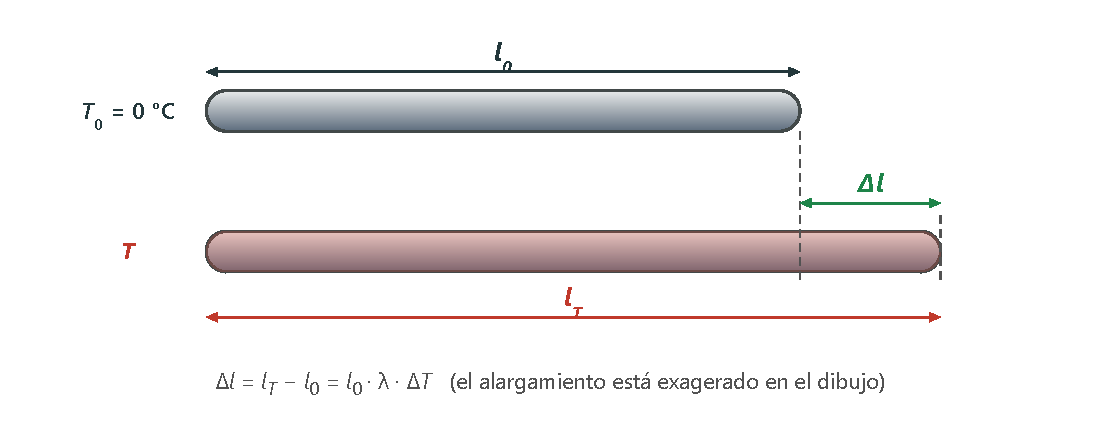
\includegraphics[width=0.85\textwidth]{images/UD12/dilatacion}
    \caption{Dilatación lineal de una barra al aumentar su temperatura.}
    \label{fig:dilatacion}
\end{figure}

\begin{definition}[Dilatación lineal]
    La \textbf{dilatación lineal} es el aumento de longitud que experimenta un cuerpo al calentarse. Si \(l_0\) es su longitud a \qty{0}{\degreeCelsius}, a la temperatura \(T\) (en \unit{\degreeCelsius}) su longitud es:
    \[ \boxed{l_T = l_0 \cdot (1 + \lambda \cdot T)} \qquad \Delta l = l_T - l_0 = l_0 \cdot \lambda \cdot T \]
    \(\lambda\) es el \textbf{coeficiente de dilatación lineal}: lo que se alarga cada metro de la sustancia, medido a \qty{0}{\degreeCelsius}, cuando su temperatura sube \qty{1}{\degreeCelsius}. Es característico de cada sustancia y se mide en \unit[per-mode=power]{\per\degreeCelsius}.
\end{definition}

En general, si la longitud inicial no está medida a \qty{0}{\degreeCelsius}, se usa la variación de temperatura: \(\Delta l = l_0 \cdot \lambda \cdot \Delta T\).

\begin{center}
    % --- tabla antigua ---
    % \begin{tblr}{colspec={lc}, hlines, vlines, row{1}={bg=ocre!85, fg=white, font=\bfseries}}
        % Sustancia & \(\lambda\) (\(\times 10^{-5}\) \unit[per-mode=power]{\per\degreeCelsius}) \\
        % Aluminio & \num{2.4} \\
        % Cobre & \num{1.8} \\
        % Hierro & \num{1.2} \\
        % Acero & \num{1.1} \\
        % Vidrio & \num{0.1}--\num{1.3} \\
        % Hormigón & \num{0.7}--\num{1.4} \\
    % \end{tblr}
    % --- tabla nueva ---
    \begin{tabular}{@{}lc@{}}
        \toprule
        \textbf{Sustancia} & \textbf{\(\lambda\) (\(\times 10^{-5}\) \unit[per-mode=power]{\per\degreeCelsius})} \\
        \midrule
        Aluminio & \num{2.4} \\[3pt]
        Cobre & \num{1.8} \\[3pt]
        Hierro & \num{1.2} \\[3pt]
        Acero & \num{1.1} \\[3pt]
        Vidrio & \num{0.1}--\num{1.3} \\[3pt]
        Hormigón & \num{0.7}--\num{1.4} \\
        \bottomrule
    \end{tabular}
\end{center}

\begin{example}
    Una barra de aluminio mide \qty{5}{\m} a \qty{0}{\degreeCelsius}. ¿Qué longitud tiene a \qty{40}{\degreeCelsius}? Dato: \(\lambda_{\text{Al}} = \qty[per-mode=power]{2.4e-5}{\per\degreeCelsius}\).
    \[ l_T = l_0 \cdot (1 + \lambda \cdot T) = 5 \cdot (1 + \num{2.4e-5} \cdot 40) = \textcolor{red}{\qty{5.0048}{\m}} \]
    La barra se ha alargado \qty{4.8}{\mm}: muy poco, pero suficiente para que haya que tenerlo en cuenta en las construcciones.
\end{example}

Los \textbf{líquidos} y los \textbf{gases} se dilatan mucho más que los sólidos. En ello se basan los termómetros de líquido: al calentarse, el mercurio o el alcohol se dilatan y suben por un tubo muy estrecho. El agua tiene un comportamiento anómalo: entre \qty{0}{\degreeCelsius} y \qty{4}{\degreeCelsius}, al calentarse se \emph{contrae}, y su densidad es máxima a \qty{4}{\degreeCelsius}. Por eso, en invierno, el fondo de los lagos se queda a unos \qty{4}{\degreeCelsius} y el hielo flota en la superficie, lo que permite que la vida acuática sobreviva.

\begin{exercise}
    Tenemos dos barras de hierro que, a \qty{0}{\degreeCelsius}, miden \qty{1.5}{\m} y \qty{3}{\m}. Calcula la longitud de la primera a \qty{80}{\degreeCelsius} y cuánto se alarga la segunda a \qty{150}{\degreeCelsius}. Dato: \(\lambda_{\text{Fe}} = \qty[per-mode=power]{1.2e-5}{\per\degreeCelsius}\).
    \begin{solu}
        \textcolor{blue}{Primera barra:} \(l_T = \num{1.5} \cdot (1 + \num{1.2e-5} \cdot 80) = \textcolor{red}{\qty{1.50144}{\m}}\).

        \textcolor{blue}{Segunda barra:} \(\Delta l = l_0 \cdot \lambda \cdot T = 3 \cdot \num{1.2e-5} \cdot 150 = \qty{5.4e-3}{\m} = \textcolor{red}{\qty{5.4}{\mm}}\).
    \end{solu}
\end{exercise}

\begin{exercise}
    Un raíl de acero mide \qty{25}{\m} a \qty{0}{\degreeCelsius}. ¿Cuánto se alarga en un día de verano en que se encuentra a \qty{45}{\degreeCelsius}? Dato: \(\lambda_{\text{acero}} = \qty[per-mode=power]{1.1e-5}{\per\degreeCelsius}\).
    \begin{solu}
        \(\Delta l = l_0 \cdot \lambda \cdot T = 25 \cdot \num{1.1e-5} \cdot 45 = \qty{0.0124}{\m} \approx \textcolor{red}{\qty{12.4}{\mm}}\); el raíl mide unos \qty{25.012}{\m}.
    \end{solu}
\end{exercise}

\begin{exercise}
    No conseguimos desenroscar la tapa metálica de un tarro de cristal. ¿Cómo podríamos lograrlo con agua caliente? Justifica tu respuesta.
    \begin{solu}
        Poniendo la tapa bajo un \textcolor{red}{chorro de agua caliente}. El metal tiene un coeficiente de dilatación mayor que el vidrio, así que la tapa \textcolor{red}{se dilata más que la boca del tarro}, queda más holgada y se puede desenroscar.
    \end{solu}
\end{exercise}

\subsection*{Actividades de consolidación: la dilatación}

\begin{exercise}
    Copia y completa: «El coeficiente de dilatación lineal del cobre es \qty[per-mode=power]{1.8e-5}{\per\degreeCelsius}. Esto quiere decir que \qty{1}{\m} de cobre, medido a \qty{0}{\degreeCelsius}, se alarga \ldots{} cuando su temperatura sube \qty{1}{\degreeCelsius}».
    \begin{solu}
        \ldots{} se alarga \textcolor{red}{\qty{1.8e-5}{\m}} (es decir, \qty{0.018}{\mm}).
    \end{solu}
\end{exercise}

\begin{exercise}
    Cuando se dilata una chapa metálica (dos dimensiones), ¿se trata de una dilatación lineal, superficial o cúbica?
    \begin{solu}
        De una dilatación \textcolor{red}{superficial}.
    \end{solu}
\end{exercise}

\begin{exercise}
    Algunos puentes son casi un metro más largos en verano que en invierno. Investiga qué se hace para que no se deformen.
    \begin{solu}
        Respuesta libre. Se construyen con \textcolor{red}{juntas de dilatación}: huecos entre tramos (a menudo cubiertos con piezas metálicas en forma de peine) que permiten que el tablero se alargue y se acorte sin deformarse. Además, el tablero se apoya sobre apoyos deslizantes o de neopreno.
    \end{solu}
\end{exercise}

\begin{exercise}
    Investiga qué efectos tiene la dilatación en las estructuras de hormigón y para qué sirven las juntas de dilatación.
    \begin{solu}
        Respuesta libre. Al calentarse y enfriarse, el hormigón se dilata y se contrae; si no tiene espacio, aparecen \textcolor{red}{tensiones que lo agrietan}. Las \textcolor{red}{juntas de dilatación} dividen la estructura en partes separadas por un pequeño hueco, de modo que cada parte puede dilatarse y contraerse libremente.
    \end{solu}
\end{exercise}

\begin{exercise}
    Investiga cómo afecta la dilatación a los raíles del tren y cómo se evitan sus efectos en la actualidad.
    \begin{solu}
        Respuesta libre. Si los raíles no pudieran alargarse, con el calor se \textcolor{red}{combarían} y el tren podría descarrilar. Antes se dejaba un pequeño \textcolor{red}{hueco entre raíles} (por eso sonaba el «traqueteo»). Hoy, en las líneas modernas, los raíles se sueldan en barras muy largas que se colocan \textcolor{red}{tensadas} y bien sujetas a las traviesas, para que no puedan dilatarse, y se usan aparatos de dilatación en algunos puntos.
    \end{solu}
\end{exercise}

\begin{exercise}
    La figura muestra la lámina bimetálica de un termostato: dos láminas de metales con distinto coeficiente de dilatación, soldadas entre sí. Explica cómo funciona.
    \begin{center}
        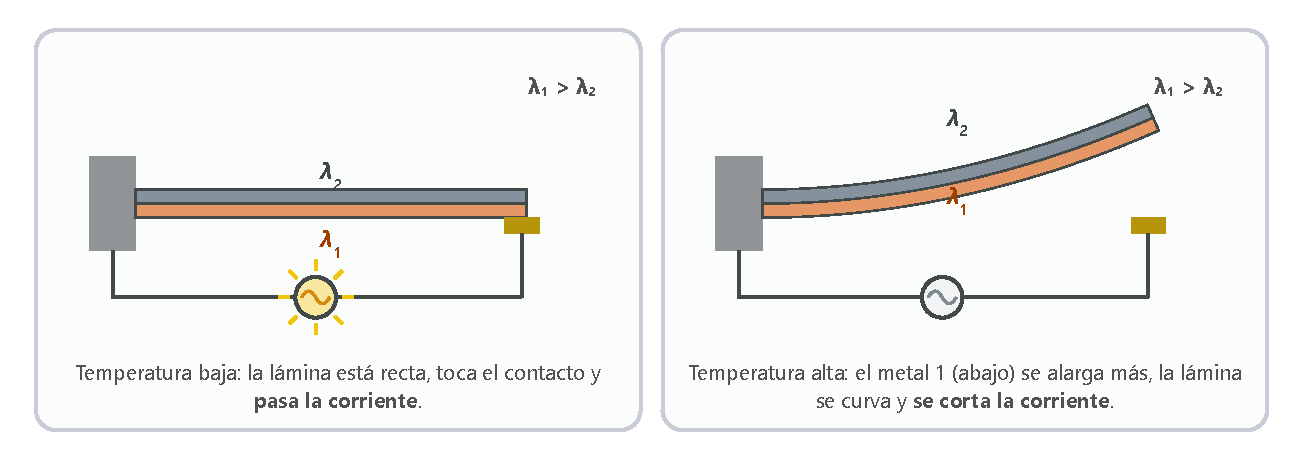
\includegraphics[width=0.9\textwidth]{images/UD12/bimetal}
    \end{center}
    \begin{solu}
        Al subir la temperatura, el metal de mayor coeficiente de dilatación (\(\lambda_1\)) se alarga más que el otro. Como están soldados, la lámina \textcolor{red}{se curva}, quedando el metal que más se dilata en la parte exterior (convexa). Al curvarse, la lámina \textcolor{red}{se separa del contacto y corta la corriente} (por ejemplo, la de la resistencia de una plancha o de un radiador). Cuando se enfría, vuelve a estar recta, cierra el circuito y la corriente pasa de nuevo. Así se mantiene la temperatura alrededor de un valor.
    \end{solu}
\end{exercise}

\begin{exercise}
    Usando la tabla de coeficientes de dilatación lineal, calcula cuánto se alarga \qty{1}{\m} de cada material cuando su temperatura sube de \qty{0}{\degreeCelsius} a \qty{40}{\degreeCelsius}.
    \begin{solu}
        \(\Delta l = l_0 \cdot \lambda \cdot T = 1 \cdot \lambda \cdot 40\):
        \begin{center}
            % --- tabla antigua ---
            % \begin{tblr}{colspec={lc}, hlines, vlines, row{1}={bg=ocre!85, fg=white, font=\bfseries}}
                % Material & \(\Delta l\) (m) \\
                % Aluminio & \num{9.6e-4} \\
                % Cobre & \num{7.2e-4} \\
                % Hierro & \num{4.8e-4} \\
                % Acero & \num{4.4e-4} \\
                % Vidrio & entre \num{4e-5} y \num{5.2e-4} \\
                % Hormigón & entre \num{2.8e-4} y \num{5.6e-4} \\
            % \end{tblr}
            % --- tabla nueva ---
            \begin{tabular}{@{}lc@{}}
                \toprule
                \textbf{Material} & \textbf{\(\Delta l\) (m)} \\
                \midrule
                Aluminio & \num{9.6e-4} \\[3pt]
                Cobre & \num{7.2e-4} \\[3pt]
                Hierro & \num{4.8e-4} \\[3pt]
                Acero & \num{4.4e-4} \\[3pt]
                Vidrio & entre \num{4e-5} y \num{5.2e-4} \\[3pt]
                Hormigón & entre \num{2.8e-4} y \num{5.6e-4} \\
                \bottomrule
            \end{tabular}
        \end{center}
    \end{solu}
\end{exercise}

%========================================================================================
\section{Equivalencia entre energía mecánica y energía térmica}
%========================================================================================

Sabemos que la combustión no es la única forma de producir energía térmica: también se obtiene a partir de la energía mecánica. Basta con frotarse las manos, frenar una bicicleta o taladrar una pieza de metal, como observó Thompson.

\subsection{¿Qué relación cuantitativa existe entre el trabajo y el calor?}

En 1845, el físico inglés \textbf{James Prescott Joule} demostró experimentalmente que el trabajo y el calor son equivalentes. En su experimento más famoso (figura~\ref{fig:joule}), unas pesas caían desde cierta altura y, al bajar, hacían girar unas paletas dentro de un recipiente con agua, aislado del exterior. El rozamiento de las paletas con el agua aumentaba su temperatura. Joule midió la energía potencial que perdían las pesas y el calor que ganaba el agua, y comprobó que, \textbf{siempre que se realiza la misma cantidad de trabajo, se obtiene la misma cantidad de calor}, tanto si el trabajo es mecánico como si es eléctrico o químico.

\begin{figure}[H]
    \centering
    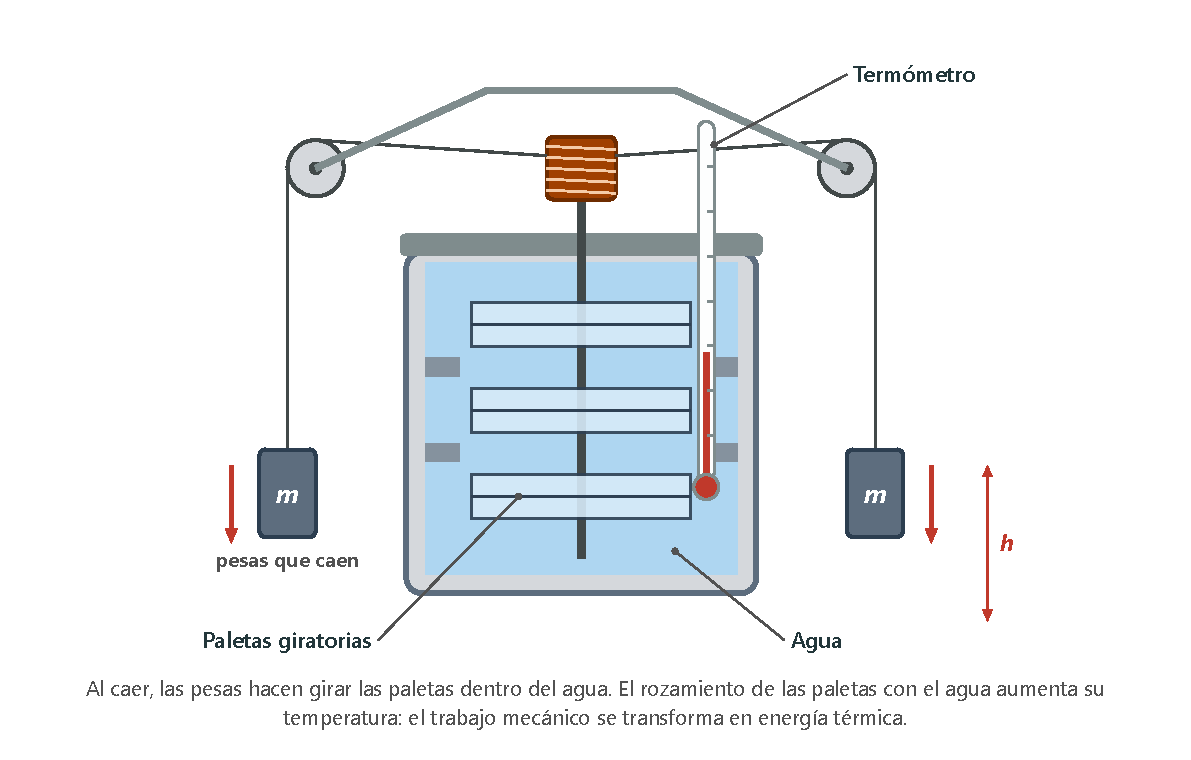
\includegraphics[width=0.85\textwidth]{images/UD12/joule}
    \caption{Experimento de Joule para demostrar la equivalencia entre trabajo y calor.}
    \label{fig:joule}
\end{figure}

\begin{definition}[Equivalente mecánico del calor]
    Si el trabajo y el calor se miden en las mismas unidades, la relación encontrada por Joule es simplemente:
    \[ W = Q \]
    Este resultado se conoce como \textbf{equivalente mecánico del calor}. Cuando el calor se medía en calorías, Joule encontró que \(\qty{1}{\calorie} = \qty{4.18}{\joule}\).
\end{definition}

El resultado de Joule es otra forma de expresar el \textbf{principio de conservación de la energía}, ahora incluyendo el calor como forma de transferir energía:

\begin{marker}
    La \textbf{energía total} de un sistema aislado permanece \textbf{constante}: la energía no se crea ni se destruye, solo se transforma o se transfiere (mediante trabajo o calor).
\end{marker}

\begin{example}
    En una cascada de \qty{50}{\m} de altura, ¿cuánto aumentaría la temperatura del agua si toda su energía potencial se transformase en energía térmica del agua al chocar abajo? (Joule intentó medirlo durante su luna de miel en Suiza.)

    Para una masa \(m\) de agua, igualamos la energía potencial perdida con el calor que gana:
    \[ m \cdot g \cdot h = m \cdot c \cdot \Delta T \Rightarrow \Delta T = \frac{g \cdot h}{c} = \frac{\num{9.8} \cdot 50}{4180} = \textcolor{red}{\qty{0.12}{\degreeCelsius}} \]
    La masa se simplifica. El aumento es muy pequeño: hace falta mucho trabajo para calentar el agua.
\end{example}

\subsection{La degradación de la energía}

\begin{marker}
    Es fácil transformar \textbf{toda} la energía mecánica en energía térmica, pero \textbf{no es posible transformar totalmente la energía térmica en energía mecánica}.
\end{marker}

Por ejemplo, el trabajo de las fuerzas de rozamiento se convierte por completo en calor. En cambio, una máquina térmica solo consigue aprovechar como trabajo una parte de la energía térmica que recibe; el resto se transfiere al ambiente. Por eso decimos que la energía se \textbf{degrada}: en cada transformación, aunque la cantidad total se conserva, una parte acaba en una forma \textbf{menos útil para realizar trabajo} (energía térmica repartida por el ambiente a baja temperatura). La energía útil siempre es menor que la energía total.

\begin{definition}[Rendimiento]
    El \textbf{rendimiento} de cualquier transformación de energía es el porcentaje de la energía total que se aprovecha:
    \[ \text{rendimiento} = \frac{\text{energía útil}}{\text{energía total}} \cdot 100 \]
\end{definition}

\begin{example}
    A una máquina se le suministran \qty{400}{\joule}, de los cuales solo aprovecha \qty{100}{\joule} como trabajo. ¿Cuál es su rendimiento?
    \[ \text{rendimiento} = \frac{100}{400} \cdot 100 = \textcolor{red}{\qty{25}{\percent}} \]
    Los \qty{300}{\joule} restantes no desaparecen: se transfieren al ambiente, sobre todo como calor.
\end{example}

\begin{exercise}
    Frota con fuerza una lima de hierro contra una superficie metálica durante unos minutos. ¿Qué les ocurre a la lima y a la superficie? ¿Qué transformación de energía se ha producido?
    \begin{solu}
        Las dos \textcolor{red}{se calientan}: el trabajo de las fuerzas de rozamiento se ha transformado en \textcolor{red}{energía térmica}.
    \end{solu}
\end{exercise}

\begin{exercise}
    ¿Puede ser del \qty{100}{\percent} el rendimiento de una máquina que transforma energía térmica en mecánica? ¿Por qué?
    \begin{solu}
        \textcolor{red}{No}. La energía térmica no puede transformarse por completo en energía mecánica: siempre se transfiere una parte al ambiente como calor, así que el rendimiento de una máquina térmica es siempre \textcolor{red}{menor del \qty{100}{\percent}}.
    \end{solu}
\end{exercise}

\subsection*{Actividades de consolidación: equivalencia entre trabajo y calor}

\begin{exercise}
    ¿Qué se conoce como equivalente mecánico del calor? ¿Quién lo determinó?
    \begin{solu}
        Es la equivalencia entre trabajo y calor: una misma cantidad de trabajo produce siempre la misma cantidad de calor. Si los dos se miden en julios, \textcolor{red}{\(W = Q\)}; con la antigua unidad de calor, \(\qty{1}{\calorie} = \qty{4.18}{\joule}\). Lo determinó \textcolor{red}{James Prescott Joule} en 1845.
    \end{solu}
\end{exercise}

\begin{exercise}
    Dobla un alambre fino varias veces por el mismo sitio. Comprueba que se calienta en esa zona e identifica la transformación de energía que se produce. ¿Puede realizarse la transformación inversa por completo?
    \begin{solu}
        Se transforma \textcolor{red}{energía mecánica (trabajo) en energía térmica}. La transformación inversa \textcolor{red}{no puede realizarse por completo}: no es posible convertir toda la energía térmica en trabajo.
    \end{solu}
\end{exercise}

\begin{exercise}
    ¿Cuál es el rendimiento de una transformación energética si de \qty{8e6}{\joule} solo se aprovechan \qty{5.2e6}{\joule}?
    \begin{solu}
        \(\text{rendimiento} = \dfrac{\num{5.2e6}}{\num{8e6}} \cdot 100 = \textcolor{red}{\qty{65}{\percent}}\).
    \end{solu}
\end{exercise}

\begin{exercise}
    Los procesos que cumplen el principio de conservación de la energía pero nunca ocurren espontáneamente al revés se llaman \textbf{irreversibles}.
    \begin{enumerate}[label=\alph*)]
        \item Al poner en contacto dos cuerpos a diferente temperatura, el caliente cede energía al frío hasta que alcanzan el equilibrio térmico. ¿Puede ocurrir espontáneamente el proceso inverso? ¿Es irreversible?
        \item Al abrir un frasco de perfume, este se evapora y se reparte por la habitación. ¿Puede ocurrir espontáneamente el proceso inverso? ¿Es irreversible?
    \end{enumerate}
    \begin{solu}
        a) \textcolor{red}{No}: nunca se ha visto que dos cuerpos a la misma temperatura se separen espontáneamente en uno caliente y otro frío. Es un \textcolor{red}{proceso irreversible}.
        b) \textcolor{red}{No}: el perfume repartido por la habitación no vuelve solo al frasco. También es \textcolor{red}{irreversible}.
    \end{solu}
\end{exercise}

\begin{exercise}
    ¿Qué significa que el rendimiento de una transformación energética es del \qty{50}{\percent}?
    \begin{solu}
        Que solo se aprovecha como energía útil \textcolor{red}{la mitad} de la energía total suministrada; la otra mitad se transfiere al ambiente, sobre todo como calor.
    \end{solu}
\end{exercise}

\begin{exercise}
    Un coche de \qty{1200}{\kg} que circula a \qty{72}{\km\per\hour} frena hasta pararse. ¿Cuánta energía cinética se transforma en energía térmica en los frenos? Si toda esa energía calentara los discos de freno (\qty{8}{\kg} de acero en total, \(c = \qty{450}{\cunit}\)), ¿cuánto subiría su temperatura?
    \begin{solu}
        \(v = \qty{72}{\km\per\hour} = \qty{20}{\m\per\s}\). \(E_c = \frac{1}{2} \cdot 1200 \cdot 20^2 = \textcolor{red}{\qty{240000}{\joule}}\).

        \(\Delta T = \dfrac{Q}{m \cdot c} = \dfrac{\num{240000}}{8 \cdot 450} \approx \textcolor{red}{\qty{67}{\degreeCelsius}}\). Por eso los frenos se calientan tanto en una bajada larga.
    \end{solu}
\end{exercise}

%========================================================================================
\section[Las máquinas térmicas]{Aplicaciones de la transformación de energía térmica en energía mecánica: las máquinas térmicas}
%========================================================================================

Una \textbf{máquina térmica} es un dispositivo que transforma en energía mecánica (trabajo) parte del calor obtenido, normalmente, de la combustión de un combustible. Toda máquina térmica funciona entre un \textbf{foco caliente} (la caldera o la cámara de combustión) y un \textbf{foco frío} (el condensador, el refrigerante o el propio ambiente).

\begin{figure}[H]
    \centering
    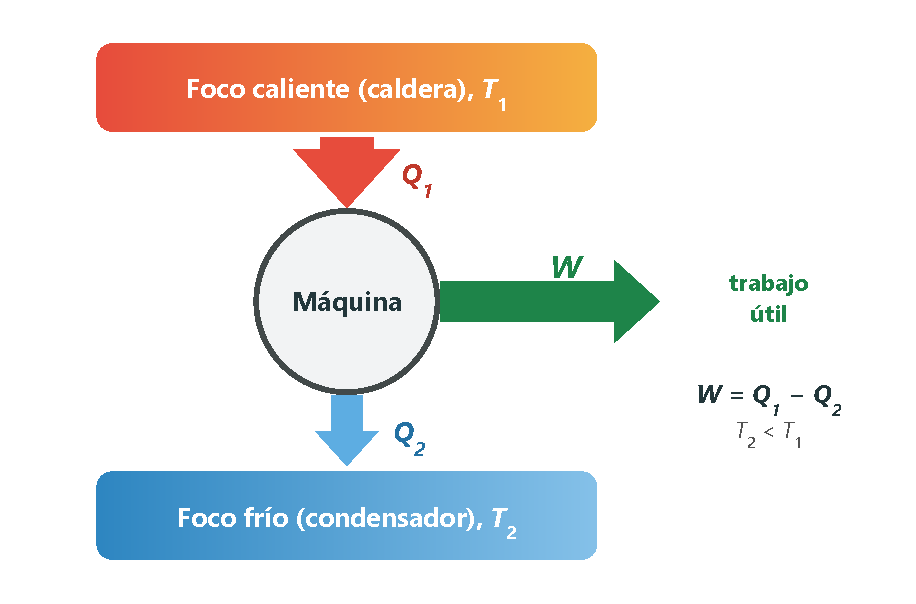
\includegraphics[width=0.7\textwidth]{images/UD12/maquina_termica}
    \caption{Esquema de funcionamiento de una máquina térmica.}
    \label{fig:maquina_termica}
\end{figure}

Como muestra la figura~\ref{fig:maquina_termica}, la máquina toma un calor \(Q_1\) del foco caliente, que está a la temperatura \(T_1\); convierte una parte en trabajo mecánico, \(W\), y cede el resto, \(Q_2\), al foco frío, que está a una temperatura menor, \(T_2\). La energía útil es:
\[ W = Q_1 - Q_2 \]

El rendimiento de la máquina térmica, \(R\), es:
\[ R = \frac{W}{Q_1} \cdot 100 = \frac{Q_1 - Q_2}{Q_1} \cdot 100 \]

El rendimiento \textbf{máximo} (teórico) que puede alcanzar una máquina térmica depende solo de las temperaturas absolutas (en kelvin) del foco caliente, \(T_1\), y del foco frío, \(T_2\):
\[ \boxed{R_{\text{máx}} = \frac{T_1 - T_2}{T_1} \cdot 100} \]
Las máquinas reales tienen siempre un rendimiento menor que este, por los rozamientos y las pérdidas de calor. Cuanto mayor es la diferencia de temperatura entre los focos, mayor es el rendimiento posible.

Según dónde se queme el combustible, las máquinas térmicas son:
\begin{itemize}
    \item De \textbf{combustión externa}: el combustible se quema fuera de la máquina, por ejemplo, en una caldera (máquina de vapor, turbina de vapor).
    \item De \textbf{combustión interna}: el combustible se quema dentro del motor (motores de gasolina y diésel, turbinas de los aviones).
\end{itemize}

\begin{example}
    Una máquina térmica recibe \qty{5000}{\joule} del foco caliente y realiza un trabajo de \qty{1500}{\joule}. ¿Cuál es su rendimiento? ¿Cuánto calor cede al foco frío?
    \[ R = \frac{W}{Q_1} \cdot 100 = \frac{1500}{5000} \cdot 100 = \textcolor{red}{\qty{30}{\percent}} \qquad Q_2 = Q_1 - W = 5000 - 1500 = \textcolor{red}{\qty{3500}{\joule}} \]
\end{example}

\subsection{La máquina de vapor}

La \textbf{máquina de vapor} es una máquina de combustión externa (figura~\ref{fig:maquina_vapor}). En una caldera se calienta agua a alta presión hasta que se convierte en vapor a muy alta temperatura. El vapor pasa al cilindro, se expande y empuja el pistón, que realiza un trabajo: mediante una biela, el movimiento de vaivén del pistón se convierte en el giro de un volante. Después, el vapor, ya más frío, pasa al condensador, donde vuelve a ser agua líquida, y una bomba la devuelve a la caldera para empezar de nuevo.

\begin{figure}[H]
    \centering
    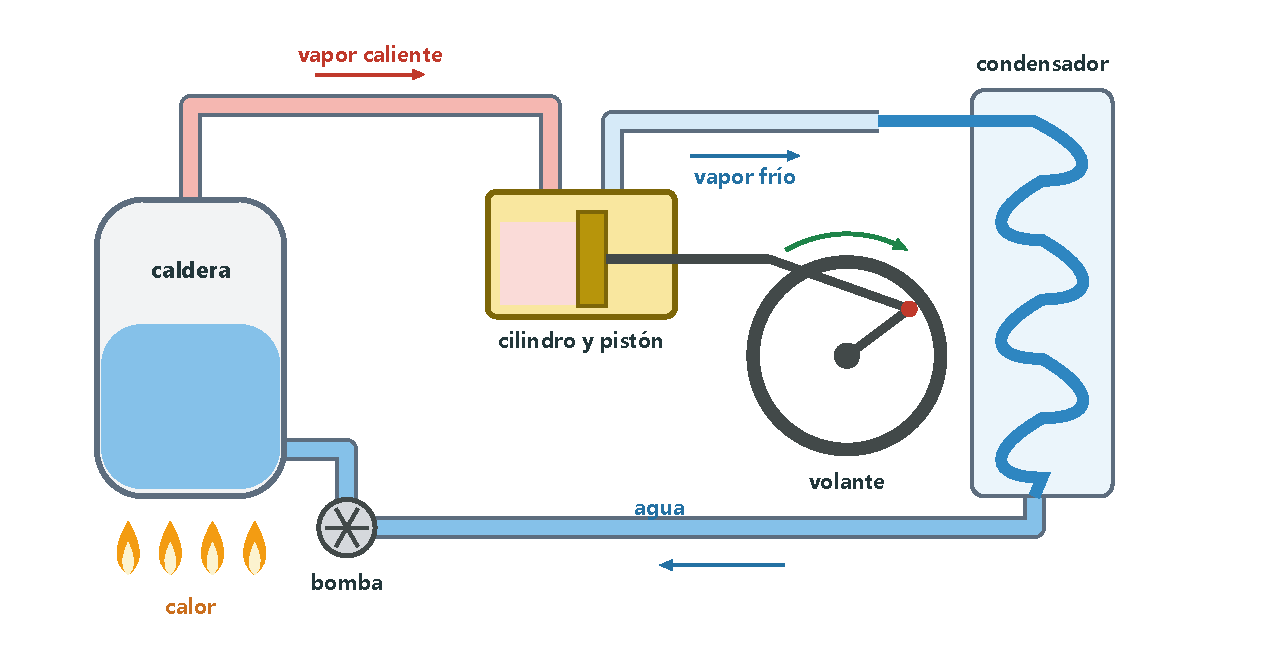
\includegraphics[width=\textwidth]{images/UD12/maquina_vapor}
    \caption{Esquema de una máquina de vapor.}
    \label{fig:maquina_vapor}
\end{figure}

La máquina de vapor, perfeccionada por James Watt a finales del siglo \textsc{xviii}, impulsó la Revolución Industrial: movió fábricas, locomotoras y barcos. Hoy se utilizan \textbf{turbinas de vapor}, que funcionan con el mismo principio en las centrales térmicas y nucleares.

\begin{example}
    Calcula el rendimiento máximo de una máquina de vapor en la que el vapor entra en el cilindro a \qty{220}{\degreeCelsius} y sale a \qty{100}{\degreeCelsius}.

    Pasamos las temperaturas a kelvin: \(T_1 = 220 + 273 = \qty{493}{\kelvin}\); \(T_2 = 100 + 273 = \qty{373}{\kelvin}\).
    \[ R = \frac{T_1 - T_2}{T_1} \cdot 100 = \frac{493 - 373}{493} \cdot 100 = \textcolor{red}{\qty{24.3}{\percent}} \]
    Incluso en el caso ideal, más de las tres cuartas partes de la energía se pierden.
\end{example}

\begin{exercise}
    Calcula el rendimiento máximo de una máquina de vapor en la que el vapor entra en el cilindro a \qty{260}{\degreeCelsius} y sale a \qty{120}{\degreeCelsius}.
    \begin{solu}
        \(T_1 = 260 + 273 = \qty{533}{\kelvin}\); \(T_2 = 120 + 273 = \qty{393}{\kelvin}\).
        \[ R = \frac{533 - 393}{533} \cdot 100 = \textcolor{red}{\qty{26.3}{\percent}} \]
    \end{solu}
\end{exercise}

\begin{exercise}
    Las máquinas de vapor de pistón han sido sustituidas por las turbinas de vapor. Busca información sobre cómo funcionan y qué ventajas tienen.
    \begin{solu}
        Respuesta libre. En una \textcolor{red}{turbina de vapor}, el vapor que sale de la caldera a gran presión pasa por unas coronas de paletas fijas, que lo dirigen, y empuja las paletas de unas ruedas móviles, que giran unidas a un eje. Ventajas: el \textcolor{red}{giro se obtiene directamente} (sin pistón ni biela), alcanzan \textcolor{red}{gran velocidad y potencia}, funcionan de forma continua, con menos vibraciones, y tienen mejor rendimiento. Se usan en las centrales eléctricas para mover los alternadores.
    \end{solu}
\end{exercise}

\subsection{El motor de combustión interna}

¿Todas las máquinas térmicas tienen caldera? No: en el \textbf{motor de combustión interna}, el combustible se quema dentro del propio cilindro. Además, la mezcla de aire y combustible se comprime antes de quemarse, lo que aumenta el rendimiento y reduce el consumo.

El más conocido es el \textbf{motor de explosión de cuatro tiempos}, que usa gasolina. Cada cilindro tiene dos orificios cerrados por válvulas: la de \textbf{admisión}, por la que entra la mezcla, y la de \textbf{escape}, por la que salen los gases quemados. En la parte superior hay una \textbf{bujía}, que produce la chispa que inicia la combustión. El pistón (o émbolo) está unido por una biela al \textbf{cigüeñal}, que transforma el movimiento de subida y bajada en giro. El motor repite cíclicamente cuatro fases o tiempos; en cada una, el pistón recorre el cilindro una vez (una carrera) y el cigüeñal da media vuelta (figura~\ref{fig:motor_cuatro_tiempos}).

\begin{figure}[H]
    \centering
    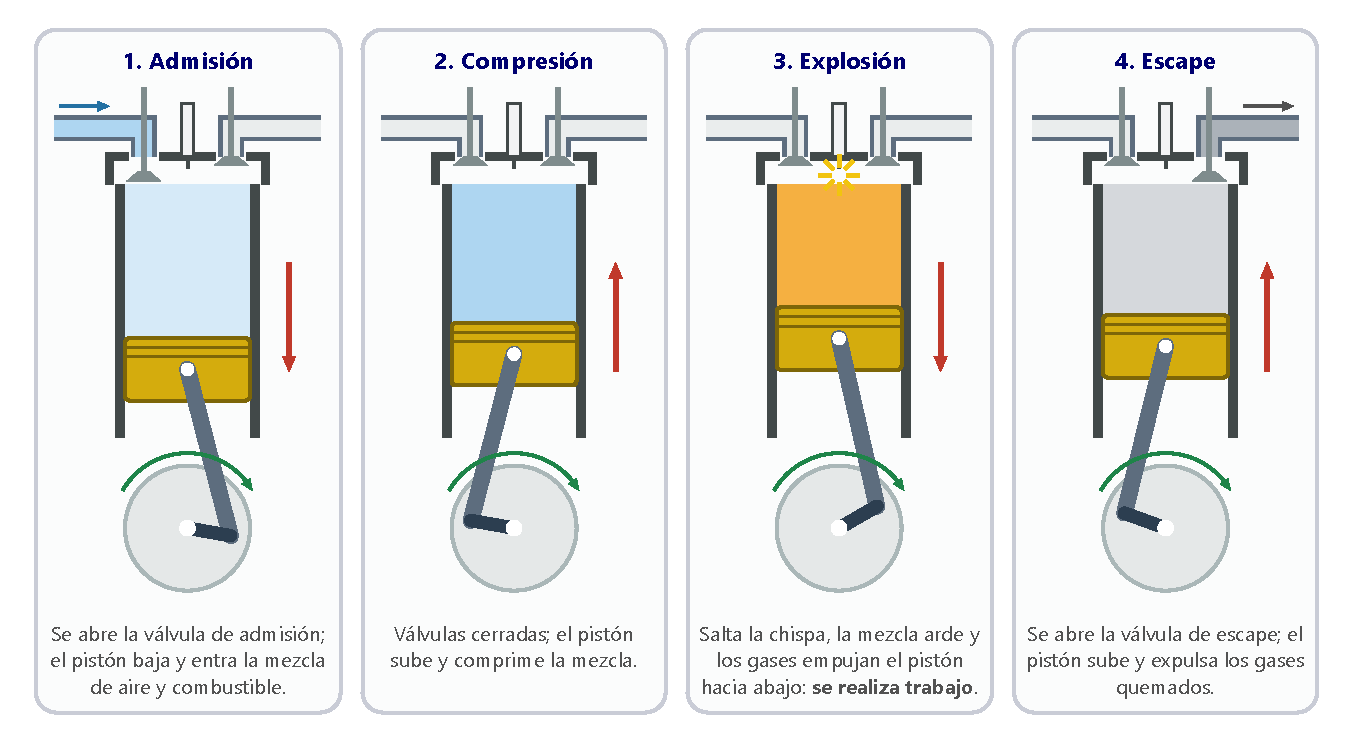
\includegraphics[width=\textwidth]{images/UD12/motor_cuatro_tiempos}
    \caption{Los cuatro tiempos de un motor de explosión.}
    \label{fig:motor_cuatro_tiempos}
\end{figure}

\begin{enumerate}[label=\numberballblue]
    \item \textbf{Admisión}. La válvula de admisión está abierta y la de escape, cerrada. El pistón baja y entra en el cilindro la mezcla de aire y gasolina. El cigüeñal gira media vuelta.
    \item \textbf{Compresión}. Las dos válvulas se cierran. El pistón sube y comprime la mezcla, que se calienta. El cigüeñal gira otra media vuelta.
    \item \textbf{Explosión} (o expansión). Con las válvulas cerradas, salta la chispa de la bujía y la mezcla se quema muy deprisa. Los gases calientes que se producen aumentan bruscamente la presión y empujan el pistón hacia abajo: es el único tiempo en el que \textbf{se realiza trabajo}. El cigüeñal gira otra media vuelta.
    \item \textbf{Escape}. Se abre la válvula de escape, el pistón sube y expulsa al exterior los gases de la combustión (sobre todo \ch{CO2} y vapor de agua). El cigüeñal gira otra media vuelta y, en total, ha dado dos vueltas completas. El ciclo vuelve a empezar.
\end{enumerate}

Los motores \textbf{diésel} también son de cuatro tiempos, pero no tienen bujía: el aire se comprime tanto que se calienta por encima de la temperatura de ignición del gasóleo, que se inyecta y arde solo.

\begin{exercise}
    ¿En cuál de los cuatro tiempos de un motor de explosión se realiza trabajo?
    \begin{solu}
        En el \textcolor{red}{tercer tiempo, la explosión}: los gases de la combustión empujan el pistón hacia abajo. En los otros tres tiempos el cigüeñal sigue girando gracias a la inercia del volante (y a los demás cilindros del motor).
    \end{solu}
\end{exercise}

\begin{exercise}
    ¿Cuántas vueltas completas da el cigüeñal durante los cuatro tiempos de un motor de explosión?
    \begin{solu}
        Media vuelta en cada tiempo: en total, \textcolor{red}{dos vueltas completas}.
    \end{solu}
\end{exercise}

\subsection*{Actividades de consolidación: las máquinas térmicas}

\begin{exercise}
    Relaciona cada tiempo del motor de combustión interna (admisión, compresión, explosión, escape) con su descripción:
    \begin{enumerate}[label=\Alph*.]
        \item Al quemarse el combustible, los gases se expanden y empujan el pistón hacia abajo.
        \item El pistón baja y permite la entrada de la mezcla de gasolina y aire.
        \item El pistón sube y empuja los gases fuera del cilindro.
        \item El pistón sube y comprime la mezcla antes de la chispa.
    \end{enumerate}
    \begin{solu}
        \textcolor{red}{Admisión: B; compresión: D; explosión: A; escape: C}.
    \end{solu}
\end{exercise}

\begin{exercise}
    ¿Qué es una máquina térmica? ¿Cuál es el rendimiento de una máquina térmica que recibe \qty{8e6}{\joule} del foco caliente y realiza un trabajo de \qty{2.8e6}{\joule}? ¿Qué calor cede al foco frío?
    \begin{solu}
        Es un dispositivo que \textcolor{red}{transforma en trabajo mecánico parte del calor} que recibe de un foco caliente, cediendo el resto a un foco frío.
        \(R = \dfrac{\num{2.8e6}}{\num{8e6}} \cdot 100 = \textcolor{red}{\qty{35}{\percent}}\); \(Q_2 = Q_1 - W = \textcolor{red}{\qty{5.2e6}{\joule}}\).
    \end{solu}
\end{exercise}

\begin{exercise}
    Calcula el rendimiento máximo de una máquina de vapor en la que el vapor entra en el cilindro a \qty{190}{\degreeCelsius} y sale a \qty{90}{\degreeCelsius}.
    \begin{solu}
        \(T_1 = \qty{463}{\kelvin}\); \(T_2 = \qty{363}{\kelvin}\). \(R = \dfrac{463 - 363}{463} \cdot 100 = \textcolor{red}{\qty{21.6}{\percent}}\).
    \end{solu}
\end{exercise}

\begin{exercise}
    ¿Por qué no se pueden usar las temperaturas en grados Celsius en la fórmula \(R = \dfrac{T_1 - T_2}{T_1} \cdot 100\)? Compruébalo con los datos de la actividad anterior.
    \begin{solu}
        Porque el numerador es una diferencia (vale lo mismo en \unit{\degreeCelsius} que en \unit{\kelvin}), pero el denominador no: hay que usar la \textcolor{red}{temperatura absoluta}. Con grados Celsius saldría \(\frac{190 - 90}{190} \cdot 100 = \qty{52.6}{\percent}\), un valor \textcolor{red}{erróneo}, mucho mayor que el real (\qty{21.6}{\percent}).
    \end{solu}
\end{exercise}


%------------------------------------------------


    \chapterimage{images/portada_cabeceras/cabecera_UD13}
    \chapter{Luz y sonido: ondas que transfieren energía}

    %! Author = crist
%! Date = 26/10/2026

\spacing{1.3}
%----------------------------------------------------------------------------------------
%	UNIDAD 13: LUZ Y SONIDO, ONDAS QUE TRANSFIEREN ENERGÍA (4.º ESO)
%   Figuras: images/UD13/*.pdf (fuente HTML en images/UD13/html, SVG en images/UD13/svg)
%   Gráficas con pgfplots: estilo «grafica», definido al inicio de la UD1/UD7.
%   Datos usados en toda la unidad: v(sonido en el aire) = 340 m/s (salvo que se indique otro valor);
%   v(sonido en el agua de mar) = 1531 m/s; c = 3·10^8 m/s; n(agua) = 1,33.
%----------------------------------------------------------------------------------------
\providecommand{\sen}{\operatorname{sen}}

% Mapa conceptual del tema (fuente en images/mapas_conceptuales/html/temas.js)
\begin{figure}[H]
    \centering
    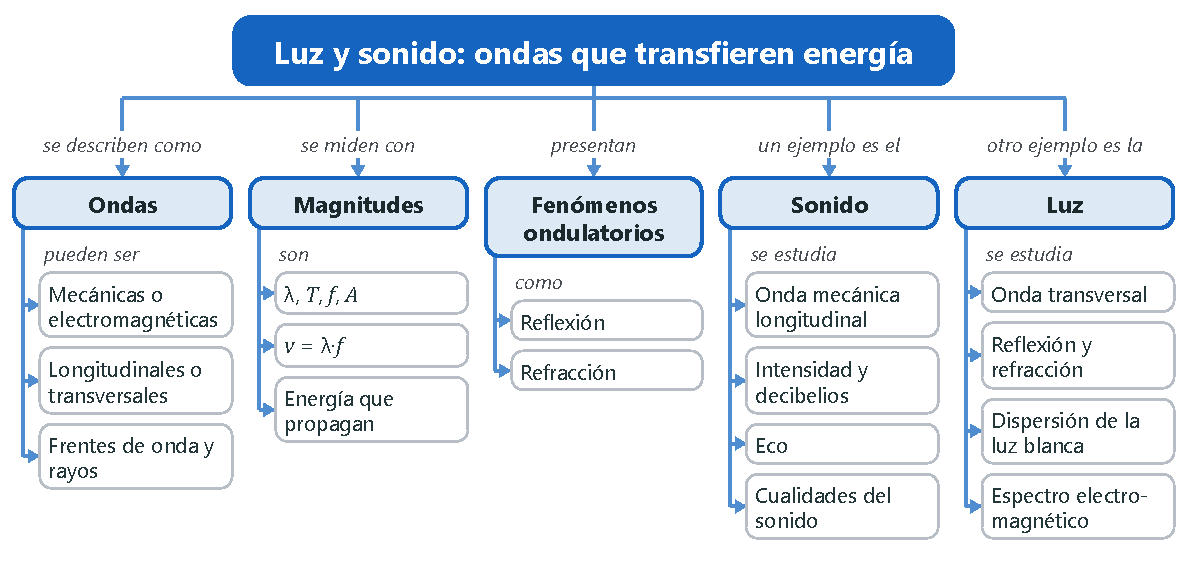
\includegraphics[width=\textwidth]{images/mapas_conceptuales/mapa_UD13}
\end{figure}

%========================================================================================
%\section*{Para empezar: la contaminación acústica}
%\addcontentsline{toc}{section}{Para empezar: la contaminación acústica}
%========================================================================================
%
%El \textbf{ruido} es cualquier sonido que no deseamos oír y que nos resulta molesto. Cuando es intenso y continuo, deteriora la calidad de vida: hablamos entonces de \textbf{contaminación acústica}. La Organización Mundial de la Salud (OMS) recomienda que el nivel de ruido ambiental en las calles no supere los \qty{65}{\decibel}, y España está entre los países más ruidosos de Europa, sobre todo por el tráfico.
%
%El ruido es un contaminante peculiar:
%\begin{itemize}
%    \item Producirlo es barato y no deja residuos: no contamina el aire, el agua ni el suelo.
%    \item Su radio de acción es pequeño comparado con el de otros contaminantes.
%    \item Solo lo percibimos por un sentido, el oído.
%\end{itemize}
%
%Sin embargo, sus efectos sobre la salud son importantes. Los \textbf{fisiológicos} pueden ser \emph{auditivos} (pérdida de audición, sordera) o \emph{no auditivos} (alteraciones del ritmo cardiaco, hipertensión, problemas de riego cerebral). Los \textbf{psicológicos} incluyen un sueño menos profundo, pérdida de memoria, estrés, irritabilidad, ansiedad o dolor de cabeza.
%
%Reducir la contaminación acústica contribuye a dos Objetivos de Desarrollo Sostenible: el \textbf{ODS 3} (\emph{Salud y bienestar}), en concreto la meta 3.4, que busca reducir la mortalidad por enfermedades no transmisibles, y el \textbf{ODS 11} (\emph{Ciudades y comunidades sostenibles}), cuya meta 11.6 pretende reducir el impacto ambiental negativo de las ciudades.
%
%En esta unidad estudiaremos qué son las \textbf{ondas}, cómo transportan energía sin transportar materia y cuáles son las propiedades de las dos ondas más presentes en nuestra vida: el \textbf{sonido} y la \textbf{luz}.
%
%\begin{exercise}
%    ¿Estás de acuerdo en que el ruido se considere un tipo de contaminación? Razona tu respuesta.
%    \begin{solu}
%        Respuesta libre. \textcolor{red}{Sí}: aunque no deja residuos, el ruido empeora la calidad de vida y tiene efectos negativos sobre la salud física y psicológica, igual que otros contaminantes.
%    \end{solu}
%\end{exercise}
%
%\begin{exercise}
%    ¿Qué ruidos contribuyen más a la contaminación acústica en tu entorno (en casa, en el instituto, en tu barrio)?
%    \begin{solu}
%        Respuesta libre. Por ejemplo: el \textcolor{red}{tráfico} de las calles cercanas, las voces y gritos en clase y en los pasillos, el volumen alto de los altavoces y auriculares, las obras, los bares o las motos.
%    \end{solu}
%\end{exercise}
%
%\begin{exercise}
%    ¿En qué se diferencia la contaminación acústica de otros tipos de contaminación, como la del aire o la del agua?
%    \begin{solu}
%        Su producción es \textcolor{red}{barata} y \textcolor{red}{no genera residuos}; su \textcolor{red}{radio de acción es pequeño}; no contamina el aire, el agua ni el suelo, y se percibe por un \textcolor{red}{único sentido}, el oído. Cuando cesa la fuente, desaparece la contaminación.
%    \end{solu}
%\end{exercise}
%
%\begin{exercise}
%    ¿Te parece adecuado que el nivel máximo recomendado de ruido ambiental sea de \qty{65}{\decibel}? ¿Debería ser mayor o menor?
%    \begin{solu}
%        Respuesta libre. Es un \textcolor{red}{límite razonable} para la calle; en lugares de descanso, de estudio o durante la noche debería ser \textcolor{red}{bastante menor} (la OMS recomienda unos \qty{35}{\decibel} en las aulas y aún menos en los dormitorios).
%    \end{solu}
%\end{exercise}
%
%\begin{exercise}
%    ¿Cuáles de los efectos del ruido sobre la salud te parecen más importantes? Clasifícalos en fisiológicos y psicológicos.
%    \begin{solu}
%        \textbf{Fisiológicos}: auditivos (pérdida de audición y sordera) y no auditivos (alteraciones del ritmo cardiaco, hipertensión arterial, afecciones en el riego cerebral). \textbf{Psicológicos}: sueño menos profundo, pérdida de memoria, estrés, irritabilidad, ansiedad, mal humor, dolor de cabeza. La importancia de cada uno es respuesta libre.
%    \end{solu}
%\end{exercise}
%
%\begin{exercise}
%    Propón tres medidas para reducir el ruido en las ciudades y relaciónalas con las metas 3.4 y 11.6 de los ODS.
%    \begin{solu}
%        Respuesta libre. Por ejemplo: \textcolor{red}{limitar el tráfico} y la velocidad en el centro, usar \textcolor{red}{asfalto} y materiales que absorban el sonido, poner \textcolor{red}{pantallas acústicas} en las vías rápidas, prohibir el claxon salvo emergencias, plantar árboles o concienciar sobre el volumen de la voz y de los aparatos. Todas mejoran la salud (meta 3.4) y reducen el impacto ambiental de las ciudades (meta 11.6).
%    \end{solu}
%\end{exercise}

%========================================================================================
\section{¿Qué es una onda? El movimiento ondulatorio}
%========================================================================================

Si tiramos una piedra a un estanque, en el punto donde cae el agua empieza a vibrar, y esa vibración se transmite a las partículas de agua vecinas: se forman círculos que se alejan del punto de impacto. Algo parecido ocurre al comprimir unas espiras de un muelle sujeto a una pared, al agitar el extremo de una cuerda, cuando vibra la membrana de un altavoz o cuando el Sol emite luz. En todos los casos, una \textbf{perturbación} producida en un punto, llamado \textbf{foco}, se \textbf{propaga} y llega a otros puntos, a los que transmite energía.

\begin{figure}[H]
    \centering
    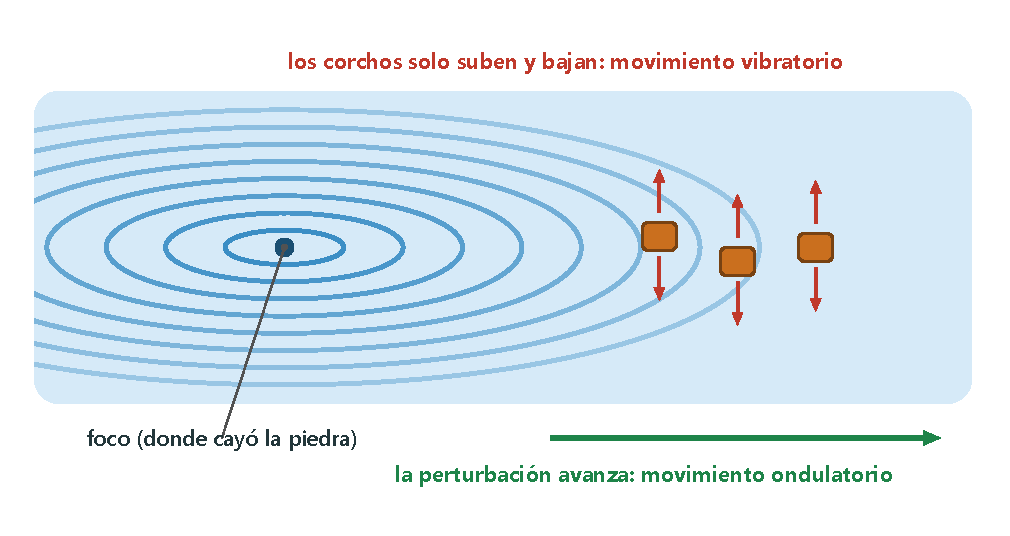
\includegraphics[width=0.75\textwidth]{images/UD13/corchos_agua}
    \caption{Unos corchos flotando en un estanque suben y bajan al llegar las ondas, pero no avanzan con ellas.}
    \label{fig:corchos_agua}
\end{figure}

Observa que los corchos de la figura~\ref{fig:corchos_agua} \emph{no se desplazan} hacia la orilla: solo suben y bajan alrededor de su posición. Lo que avanza no es el agua, sino la perturbación y, con ella, la energía.

\begin{definition}[Movimiento ondulatorio y onda]
    El \textbf{movimiento ondulatorio} es la propagación de un movimiento vibratorio (una perturbación) de unos puntos a otros de un medio. Es una forma de \textbf{transmitir energía sin transportar materia}.

    Una \textbf{onda} es la forma que adopta en cada instante la perturbación que se propaga.
\end{definition}

\begin{exercise}
    En la figura~\ref{fig:corchos_agua}, ¿qué movimiento es el vibratorio y cuál es el ondulatorio?
    \begin{solu}
        El \textcolor{red}{movimiento vibratorio} es el de cada corcho (y cada partícula de agua), que sube y baja alrededor de su posición de equilibrio. El \textcolor{red}{movimiento ondulatorio} es la propagación de esa vibración por la superficie del agua, alejándose del foco.
    \end{solu}
\end{exercise}

\begin{exercise}
    Si la onda no transporta materia, ¿cómo podemos saber que transporta energía? Pon un ejemplo.
    \begin{solu}
        Porque al llegar a un cuerpo \textcolor{red}{lo pone en movimiento} o lo modifica: las olas mueven una barca, el sonido hace vibrar el tímpano o los cristales de una ventana, y la luz del Sol calienta la piel.
    \end{solu}
\end{exercise}

\subsection{¿Cómo se clasifican las ondas?}

\textbf{Según necesiten o no un medio material para propagarse}:
\begin{itemize}
    \item \textbf{Ondas mecánicas}: se originan al perturbar un \emph{medio elástico} (sólido, líquido o gas) y \textbf{no pueden propagarse en el vacío}. Son mecánicas las ondas en la superficie del agua, el sonido y las ondas en cuerdas y muelles.
    \item \textbf{Ondas electromagnéticas}: \textbf{pueden propagarse en el vacío}, aunque también lo hacen por muchos medios materiales. Son ondas electromagnéticas la luz visible, los rayos X, los rayos ultravioleta e infrarrojos, las microondas y las ondas de radio.
\end{itemize}

\textbf{Según la relación entre la dirección de vibración y la de propagación}:
\begin{itemize}
    \item \textbf{Ondas transversales}: las partículas vibran \textbf{perpendicularmente} a la dirección en que avanza la onda. Forman una sucesión de \textbf{crestas} y \textbf{valles}. Son transversales las ondas en una cuerda, en la superficie del agua y las ondas electromagnéticas.
    \item \textbf{Ondas longitudinales}: las partículas vibran \textbf{en la misma dirección} en que avanza la onda. Forman una sucesión de \textbf{compresiones} y \textbf{dilataciones}. Son longitudinales el sonido y las compresiones que se propagan por un muelle.
\end{itemize}

\begin{figure}[H]
    \centering
    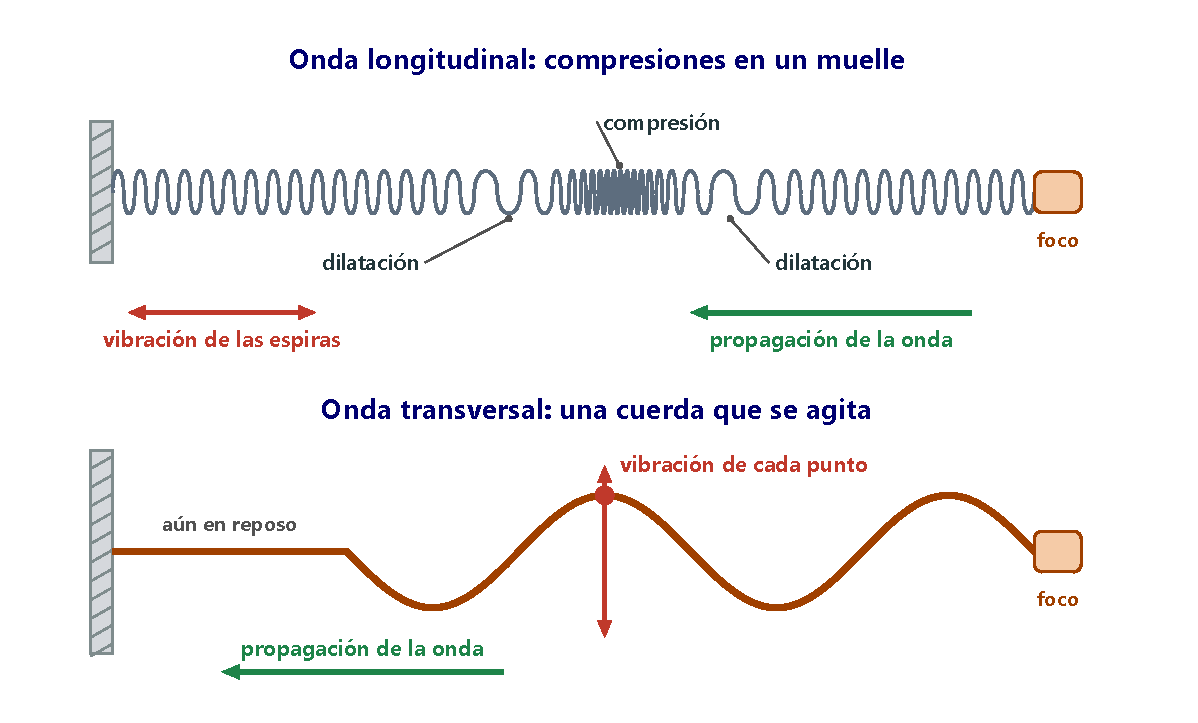
\includegraphics[width=0.9\textwidth]{images/UD13/tipos_ondas}
    \caption{Arriba, una onda longitudinal: las espiras vibran en la misma dirección en que avanza la compresión. Abajo, una onda transversal: cada punto de la cuerda sube y baja mientras la onda avanza en horizontal.}
    \label{fig:tipos_ondas}
\end{figure}

\begin{exercise}
    Indica si son verdaderas o falsas estas afirmaciones y justifícalo:
    \begin{enumerate}[label=\alph*)]
        \item Las ondas mecánicas necesitan un medio material para propagarse.
        \item Las ondas electromagnéticas no pueden propagarse por medios materiales.
        \item El sonido puede viajar por el vacío.
    \end{enumerate}
    \begin{solu}
        a) \textcolor{red}{Verdadera}: se propagan porque las partículas del medio se transmiten la vibración unas a otras. b) \textcolor{red}{Falsa}: pueden propagarse en el vacío, pero también por muchos medios materiales (la luz atraviesa el aire, el agua o el vidrio). c) \textcolor{red}{Falsa}: el sonido es una onda mecánica y necesita un medio material.
    \end{solu}
\end{exercise}

\subsection{¿Qué es un frente de onda? ¿Y un rayo?}

Cuando una onda se propaga en todas las direcciones desde un foco, todos los puntos que están a la misma distancia del foco son alcanzados a la vez por la perturbación.

\begin{definition}[Frente de onda y rayo]
    Un \textbf{frente de onda} es la línea o la superficie formada por todos los puntos alcanzados por la perturbación en el mismo instante.

    Un \textbf{rayo} es una línea imaginaria perpendicular a los frentes de onda que indica la dirección de propagación.
\end{definition}

Cerca de un foco puntual, los frentes de onda son esferas (o circunferencias en la superficie del agua); muy lejos del foco, un trozo de esa esfera es casi plano y se habla de \textbf{frentes de onda planos}, cuyos rayos son paralelos.

\begin{figure}[H]
    \centering
    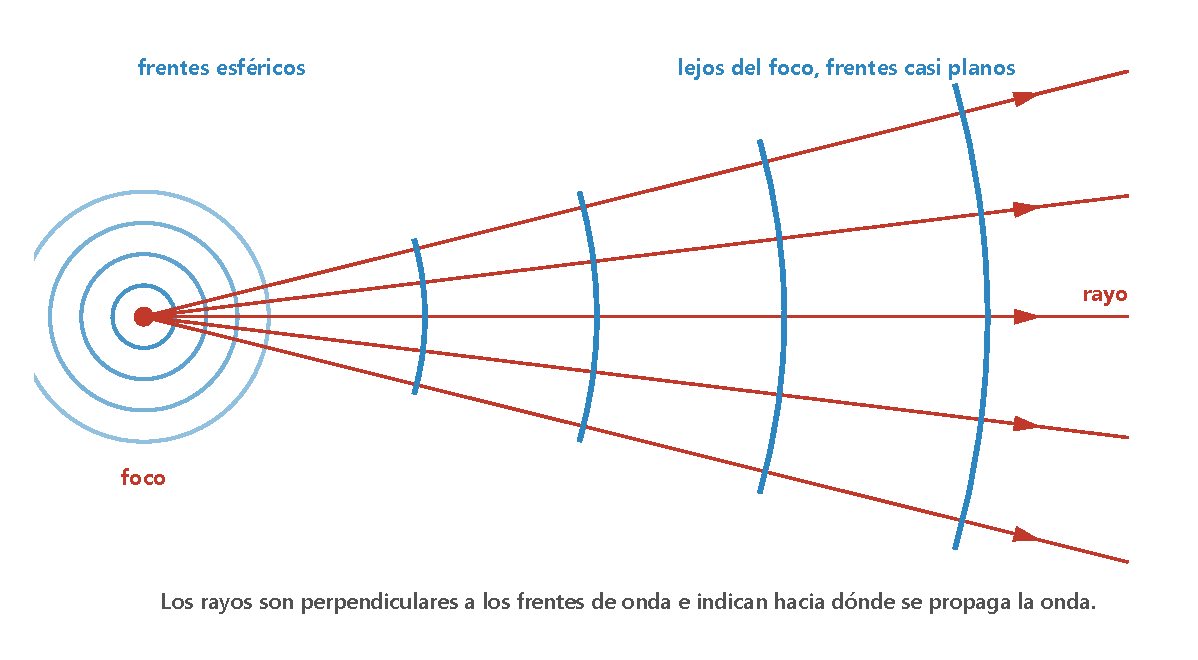
\includegraphics[width=0.85\textwidth]{images/UD13/frentes_rayos}
    \caption{Frentes de onda esféricos cerca del foco y casi planos lejos de él. Los rayos son perpendiculares a los frentes.}
    \label{fig:frentes_rayos}
\end{figure}

\begin{exercise}
    Un frente de onda plano avanza hacia la derecha. ¿Cómo son sus rayos? ¿Y si el frente avanza hacia abajo?
    \begin{solu}
        Los rayos son \textcolor{red}{rectas paralelas entre sí y perpendiculares al frente}, con el sentido de la propagación: si el frente avanza hacia la derecha (es un plano vertical), los rayos son \textcolor{red}{horizontales} y apuntan a la derecha; si avanza hacia abajo (el frente es horizontal), los rayos son \textcolor{red}{verticales} y apuntan hacia abajo.
    \end{solu}
\end{exercise}

\subsection{¿Cuáles son las magnitudes características de las ondas?}

\begin{figure}[H]
    \centering
    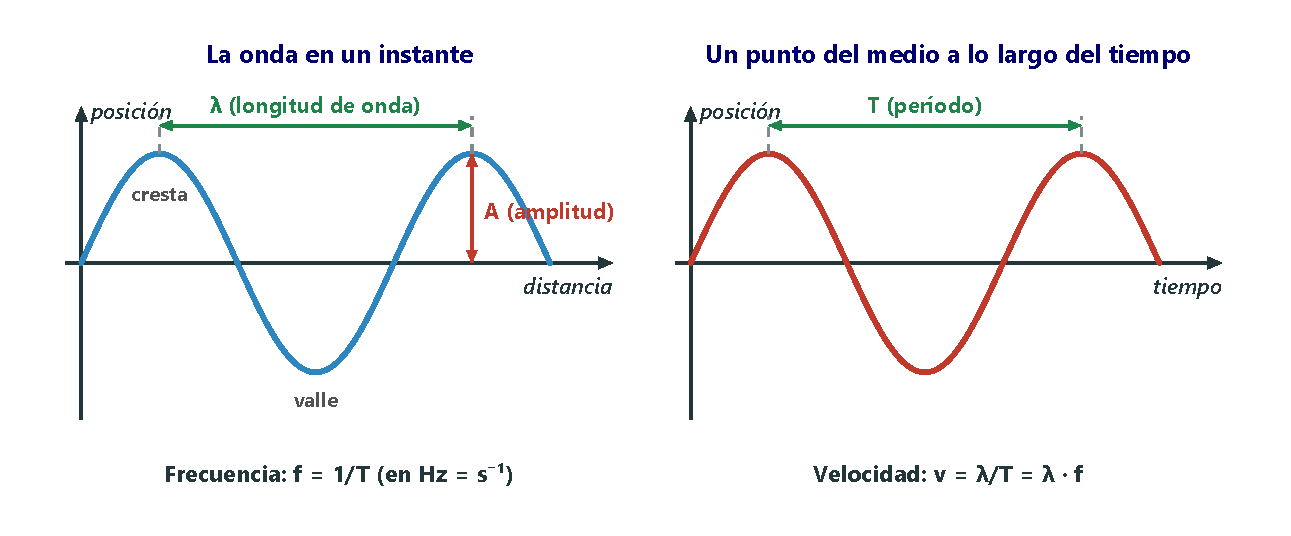
\includegraphics[width=\textwidth]{images/UD13/magnitudes_onda}
    \caption{Izquierda: la onda en un instante, con su amplitud y su longitud de onda. Derecha: la posición de un punto del medio a lo largo del tiempo, que se repite cada período.}
    \label{fig:magnitudes_onda}
\end{figure}

\begin{itemize}
    \item La \textbf{amplitud}, \(A\), es la separación máxima de cada punto del medio respecto de su posición de equilibrio. Se mide en metros.
    \item La \textbf{longitud de onda}, \(\lambda\), es la distancia entre dos puntos consecutivos que vibran exactamente igual (por ejemplo, dos crestas o dos valles seguidos). Es la distancia que avanza la onda mientras el foco realiza una vibración completa. Se mide en metros.
    \item El \textbf{período}, \(T\), es el tiempo que tarda un punto en hacer una vibración completa, que coincide con el que tarda la onda en avanzar una longitud de onda. Se mide en segundos.
    \item La \textbf{frecuencia}, \(f\), es el número de vibraciones que realiza cada punto en un segundo. Es la inversa del período, \(f = 1/T\), y se mide en \textbf{hercios} (\unit{\hertz}): \(\qty{1}{\hertz} = \qty{1}{\per\s}\).
\end{itemize}

\subsection{¿A qué velocidad se propagan las ondas?}

Si el medio tiene las mismas propiedades en todas las direcciones (es \textbf{isótropo}), la onda avanza con \textbf{velocidad constante}, es decir, con movimiento uniforme. La \textbf{velocidad de propagación}, \(v\), es la distancia que recorre la onda en cada unidad de tiempo:
\[ v = \frac{\text{distancia recorrida}}{\text{tiempo empleado}} \]

\begin{example}
    En el centro de una piscina circular de \qty{6}{\m} de radio se produce una perturbación en la superficie del agua, que tarda \qty{10}{\s} en llegar al borde. ¿A qué velocidad se propaga la onda?
    \[ v = \frac{\text{distancia}}{\text{tiempo}} = \frac{\qty{6}{\m}}{\qty{10}{\s}} = \textcolor{red}{\qty{0.6}{\m\per\s}} \]
\end{example}

\subsection{¿Cómo se relacionan las magnitudes de una onda?}

En un período, \(T\), la onda avanza exactamente una longitud de onda, \(\lambda\). Por tanto, su velocidad es \(v = \lambda / T\). Como la frecuencia es la inversa del período, obtenemos la \textbf{ecuación fundamental de las ondas}:
\begin{equation*}
    \boxed{v = \frac{\lambda}{T} = \lambda \cdot f}
\end{equation*}

\begin{remark}
    La velocidad de una onda depende del \textbf{medio} por el que se propaga, no del foco. La frecuencia, en cambio, la fija el \textbf{foco}. Por eso, cuando una onda pasa de un medio a otro, su frecuencia no cambia, pero sí su velocidad y su longitud de onda.
\end{remark}

\begin{example}
    Por una cuerda tensa se propaga, a \qty{25}{\m\per\s}, una onda de \qty{0.5}{\m} de longitud de onda. Calcula su frecuencia y su período.
    \[ f = \frac{v}{\lambda} = \frac{\qty{25}{\m\per\s}}{\qty{0.5}{\m}} = \textcolor{red}{\qty{50}{\hertz}}; \qquad T = \frac{1}{f} = \frac{1}{\qty{50}{\hertz}} = \textcolor{red}{\qty{0.02}{\s}} \]
\end{example}

\begin{exercise}
    Por una cuerda se propaga, a \qty{12}{\m\per\s}, un tren de ondas de \qty{1.5}{\m} de longitud de onda. ¿Cuáles son su frecuencia y su período?
    \begin{solu}
        \(f = \dfrac{v}{\lambda} = \dfrac{12}{\num{1.5}} = \textcolor{red}{\qty{8}{\hertz}}\); \(T = \dfrac{1}{f} = \dfrac{1}{8} = \textcolor{red}{\qty{0.125}{\s}}\).
    \end{solu}
\end{exercise}

\begin{exercise}
    Una emisora de radio de FM emite con una frecuencia de \qty{100}{\mega\hertz}. Si las ondas de radio viajan a \qty{3e8}{\m\per\s}, ¿cuál es su longitud de onda?
    \begin{solu}
        \(\lambda = \dfrac{v}{f} = \dfrac{\num{3e8}}{\num{1e8}} = \textcolor{red}{\qty{3}{\m}}\).
    \end{solu}
\end{exercise}

\subsection{Las ondas propagan energía}

En un movimiento ondulatorio se propaga energía, pero no materia. Para medir la rapidez con la que la onda transporta energía a través de una superficie se define la intensidad.

\begin{definition}[Intensidad de una onda]
    La \textbf{intensidad}, \(I\), de una onda es la energía que atraviesa cada unidad de superficie, colocada perpendicularmente a la dirección de propagación, en cada unidad de tiempo. Equivale a la potencia por unidad de superficie y se mide en \unit{\watt\per\square\m}:
    \[ I = \frac{E}{t \cdot S} = \frac{P}{S} \]
\end{definition}

Si un foco emite por igual en todas las direcciones, a una distancia \(r\) la energía se reparte sobre una esfera de superficie \(S = 4\pi r^2\). Por tanto:
\begin{equation*}
    \boxed{I = \frac{P}{4\pi r^2}}
\end{equation*}
La intensidad es \textbf{inversamente proporcional al cuadrado de la distancia} al foco: al doble de distancia, la intensidad es la cuarta parte; al triple, la novena parte.

\begin{figure}[H]
    \centering
    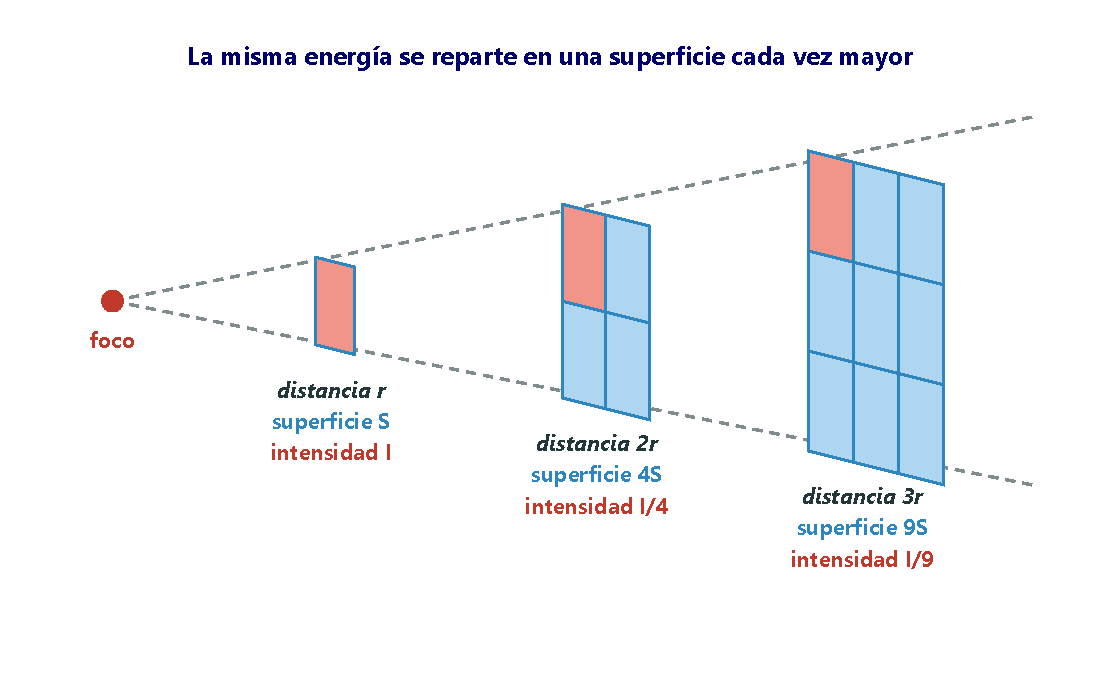
\includegraphics[width=0.75\textwidth]{images/UD13/intensidad_distancia}
    \caption{Al alejarse del foco, la misma energía se reparte en una superficie mayor y la intensidad disminuye.}
    \label{fig:intensidad_distancia}
\end{figure}

\begin{example}
    Un altavoz emite una potencia sonora de \qty{2}{\watt} por igual en todas las direcciones. ¿Con qué intensidad llega el sonido a \qty{5}{\m}? ¿Y a \qty{10}{\m}?
    \[ I_1 = \frac{P}{4\pi r^2} = \frac{\qty{2}{\watt}}{4\pi \cdot (\qty{5}{\m})^2} = \textcolor{red}{\qty{6.4e-3}{\watt\per\square\m}} \]
    Al doble de distancia, la intensidad es la cuarta parte: \(I_2 = I_1/4 = \textcolor{red}{\qty{1.6e-3}{\watt\per\square\m}}\).
\end{example}

\subsection{Fenómenos ondulatorios: reflexión y refracción}

Para explicar qué ocurre cuando una onda llega a un obstáculo o a otro medio, usamos los rayos y la \textbf{normal}, una recta perpendicular a la superficie en el punto donde llega el rayo. El \textbf{ángulo de incidencia}, \(i\), es el que forma el rayo incidente con la normal.

\begin{definition}[Reflexión]
    La \textbf{reflexión} es el cambio de dirección que experimenta una onda al chocar con una superficie sin atravesarla. La onda reflejada sigue en el mismo medio y, por tanto, con la misma velocidad.
\end{definition}

\begin{marker}
    \textbf{Leyes de la reflexión}
    \begin{itemize}
        \item El rayo incidente, la normal y el rayo reflejado están en el mismo plano.
        \item El ángulo de incidencia es igual al ángulo de reflexión (el que forma el rayo reflejado con la normal): \(\hat{\imath} = \hat{r}\).
    \end{itemize}
\end{marker}

\begin{definition}[Refracción]
    La \textbf{refracción} es el cambio de velocidad, y en general de dirección, que experimenta una onda al pasar de un medio a otro en el que se propaga con distinta velocidad.
\end{definition}

\begin{figure}[H]
    \centering
    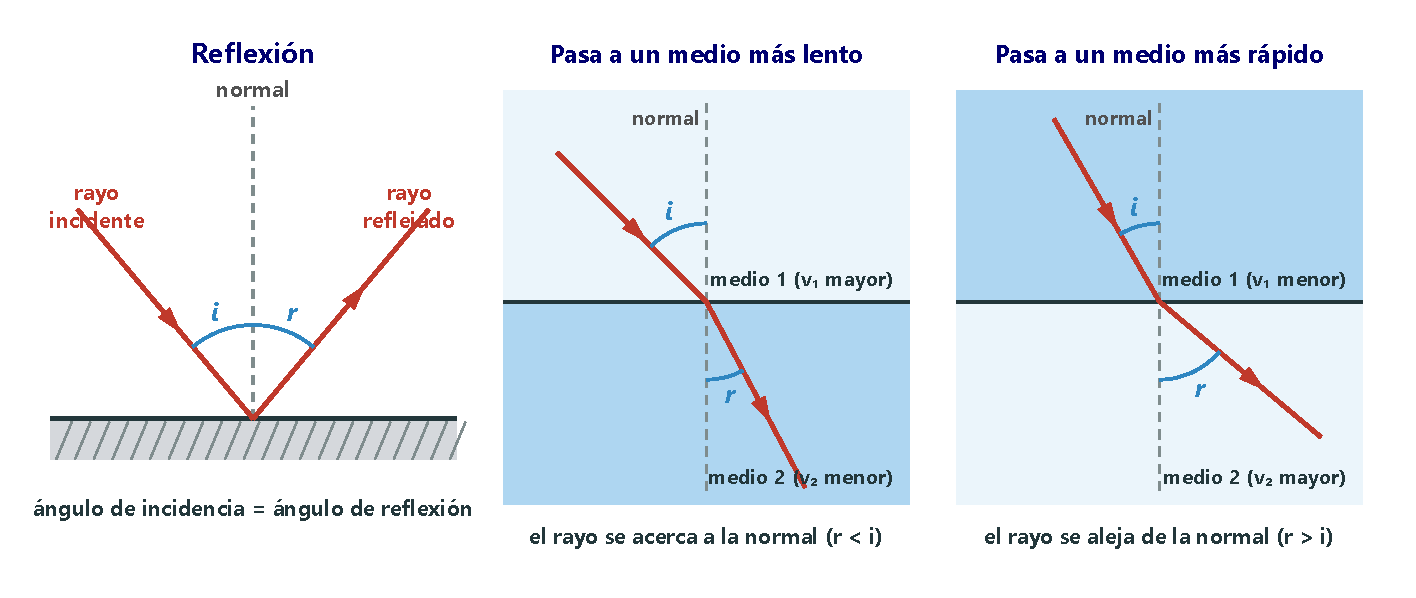
\includegraphics[width=\textwidth]{images/UD13/reflexion_refraccion}
    \caption{Reflexión (izquierda) y refracción de una onda al pasar a un medio en el que es más lenta (centro) o más rápida (derecha).}
    \label{fig:reflexion_refraccion}
\end{figure}

\begin{marker}
    \textbf{Leyes de la refracción}
    \begin{itemize}
        \item El rayo incidente, la normal y el rayo refractado están en el mismo plano.
        \item Si la onda pasa a un medio en el que se propaga \textbf{más despacio}, el rayo refractado \textbf{se acerca a la normal}. Si pasa a un medio en el que va \textbf{más deprisa}, \textbf{se aleja de la normal}.
        \item Si la onda llega \textbf{perpendicularmente} a la superficie de separación, no se desvía: sigue en línea recta (aunque cambia su velocidad).
    \end{itemize}
\end{marker}

\begin{exercise}
    Un rayo llega a una superficie formando \ang{35} con la normal. ¿Qué ángulo forma el rayo reflejado con la normal? ¿Y con la superficie?
    \begin{solu}
        Con la normal, \textcolor{red}{\ang{35}} (ley de la reflexión). Con la superficie, \(\ang{90} - \ang{35} = \textcolor{red}{\ang{55}}\).
    \end{solu}
\end{exercise}

%----------------------------------------------------------------------------------------
\subsection*{Actividades de consolidación: el movimiento ondulatorio}
%----------------------------------------------------------------------------------------

\begin{exercise}
    Clasifica estas ondas según necesiten o no un medio material y según sean transversales o longitudinales:
    \begin{enumerate}[label=\alph*)]
        \item Las ondas en la superficie de un lago.
        \item El sonido.
        \item Las ondas en una cuerda de guitarra.
        \item La luz.
        \item Las compresiones que recorren un muelle.
    \end{enumerate}
    \begin{solu}
        a) \textcolor{red}{Mecánica y transversal}. b) \textcolor{red}{Mecánica y longitudinal}. c) \textcolor{red}{Mecánica y transversal}. d) \textcolor{red}{Electromagnética y transversal}. e) \textcolor{red}{Mecánica y longitudinal}.
    \end{solu}
\end{exercise}

\begin{exercise}
    Sujetamos un extremo de un muelle a la pared y comprimimos unas espiras del otro extremo. Describe en cuatro pasos lo que ocurre a continuación.
    \begin{solu}
        1) Las espiras comprimidas empujan a las siguientes. 2) La \textcolor{red}{compresión avanza} por el muelle hacia la pared, mientras las espiras que ya ha pasado vuelven a su posición. 3) Cada espira solo \textcolor{red}{vibra adelante y atrás}, en la misma dirección en que avanza la compresión. 4) La compresión llega a la pared: se ha propagado la perturbación (y la energía), pero \textcolor{red}{no la materia} del muelle. Es una onda longitudinal.
    \end{solu}
\end{exercise}

\begin{exercise}
    Relaciona cada concepto con su definición:
    \begin{center}
        % --- tabla antigua ---
        % \begin{tblr}{colspec={lX}, width=\linewidth, hlines, vlines, row{1}={bg=ocre!85, fg=white, font=\bfseries}, cells={font=\small}}
            % Concepto & Definición \\
            % a) Movimiento ondulatorio & 1. Onda en la que las partículas vibran en la dirección de propagación. \\
            % b) Onda & 2. Propagación de un movimiento vibratorio. \\
            % c) Onda longitudinal & 3. Onda que necesita un medio material. \\
            % d) Frente de onda & 4. Onda en la que las partículas vibran perpendicularmente a la dirección de propagación. \\
            % e) Longitud de onda & 5. Superficie formada por los puntos alcanzados por la perturbación en el mismo instante. \\
            % f) Rayo & 6. Línea perpendicular al frente de onda. \\
            % g) Onda mecánica & 7. Separación máxima de un punto respecto de su posición de equilibrio. \\
            % h) Período & 8. Distancia entre dos puntos consecutivos que vibran de la misma manera. \\
            % i) Onda transversal & 9. Forma que adopta en cada instante la perturbación. \\
            % j) Amplitud & 10. Tiempo que tarda la perturbación en recorrer una longitud de onda. \\
        % \end{tblr}
        % --- tabla nueva ---
        {\small
        \begin{tabular}{@{}l p{0.78\linewidth}@{}}
            \toprule
            \textbf{Concepto} & \textbf{Definición} \\
            \midrule
            a) Movimiento ondulatorio & 1. Onda en la que las partículas vibran en la dirección de propagación. \\[3pt]
            b) Onda & 2. Propagación de un movimiento vibratorio. \\[3pt]
            c) Onda longitudinal & 3. Onda que necesita un medio material. \\[3pt]
            d) Frente de onda & 4. Onda en la que las partículas vibran perpendicularmente a la dirección de propagación. \\[3pt]
            e) Longitud de onda & 5. Superficie formada por los puntos alcanzados por la perturbación en el mismo instante. \\[3pt]
            f) Rayo & 6. Línea perpendicular al frente de onda. \\[3pt]
            g) Onda mecánica & 7. Separación máxima de un punto respecto de su posición de equilibrio. \\[3pt]
            h) Período & 8. Distancia entre dos puntos consecutivos que vibran de la misma manera. \\[3pt]
            i) Onda transversal & 9. Forma que adopta en cada instante la perturbación. \\[3pt]
            j) Amplitud & 10. Tiempo que tarda la perturbación en recorrer una longitud de onda. \\
            \bottomrule
        \end{tabular}
        }
    \end{center}
    \begin{solu}
        \textcolor{red}{a-2, b-9, c-1, d-5, e-8, f-6, g-3, h-10, i-4, j-7}.
    \end{solu}
\end{exercise}

\begin{exercise}
    Un punto de un medio vibra con un período de \qty{0.04}{\s}.
    \begin{enumerate}[label=\alph*)]
        \item ¿Cuál es su frecuencia?
        \item ¿Cuántas vibraciones completa en un minuto y medio?
    \end{enumerate}
    \begin{solu}
        a) \(f = \dfrac{1}{T} = \dfrac{1}{\num{0.04}} = \textcolor{red}{\qty{25}{\hertz}}\).
        b) En \qty{90}{\s}: \(25 \cdot 90 = \textcolor{red}{2250}\) vibraciones.
    \end{solu}
\end{exercise}

\begin{exercise}
    En la superficie de un estanque se forman ondas de \qty{4}{\cm} de longitud de onda con una frecuencia de \qty{12}{\hertz}. ¿A qué velocidad se propagan?
    \begin{solu}
        \(v = \lambda \cdot f = \num{0.04} \cdot 12 = \textcolor{red}{\qty{0.48}{\m\per\s}}\).
    \end{solu}
\end{exercise}

\begin{exercise}
    Una onda de radio tiene una frecuencia de \qty{1.5e7}{\hertz} y una longitud de onda de \qty{20}{\m}. ¿A qué velocidad se propaga? ¿Te resulta familiar el resultado?
    \begin{solu}
        \(v = \lambda \cdot f = 20 \cdot \num{1.5e7} = \textcolor{red}{\qty{3e8}{\m\per\s}}\). Es la \textcolor{red}{velocidad de la luz}: las ondas de radio son ondas electromagnéticas, como la luz.
    \end{solu}
\end{exercise}

\begin{exercise}
    ¿Cuál es la frecuencia de una onda de \qty{5}{\cm} de longitud de onda que se propaga a \qty{200}{\m\per\s}?
    \begin{solu}
        \(f = \dfrac{v}{\lambda} = \dfrac{200}{\num{0.05}} = \textcolor{red}{\qty{4000}{\hertz}}\).
    \end{solu}
\end{exercise}

\begin{exercise}
    Un avión emite un sonido con una potencia de \qty{2500}{\watt}. ¿Con qué intensidad llega ese sonido a \qty{2}{\km} de distancia?
    \begin{solu}
        \(I = \dfrac{P}{4\pi r^2} = \dfrac{2500}{4\pi \cdot (\num{2000})^2} = \dfrac{2500}{\num{5.03e7}} = \textcolor{red}{\qty{5.0e-5}{\watt\per\square\m}}\).
    \end{solu}
\end{exercise}

\begin{exercise}
    El Sol emite una potencia aproximada de \qty{3e20}{\mega\watt}. ¿Qué intensidad de radiación llega a la Tierra, si la distancia media entre ambos es de \qty{1.5e11}{\m}?
    \begin{solu}
        \(P = \qty{3e26}{\watt}\). \(I = \dfrac{P}{4\pi r^2} = \dfrac{\num{3e26}}{4\pi \cdot (\num{1.5e11})^2} = \dfrac{\num{3e26}}{\num{2.83e23}} \approx \textcolor{red}{\qty{1060}{\watt\per\square\m}}\). (Es un valor aproximado: la potencia real del Sol es algo mayor y, en la parte alta de la atmósfera, llegan unos \qty{1360}{\watt\per\square\m}.)
    \end{solu}
\end{exercise}

\begin{exercise}
    Dibuja tres ondas que se propaguen a la misma velocidad: una de mayor frecuencia, otra de mayor longitud de onda y otra de mayor amplitud que una onda de referencia.
    \begin{solu}
        Como \(v = \lambda \cdot f\) es la misma para todas, la de \textcolor{red}{mayor frecuencia tiene menor longitud de onda} (crestas más juntas) y la de \textcolor{red}{mayor longitud de onda tiene menor frecuencia}. La amplitud es independiente: basta con dibujar crestas más altas.
        \begin{center}
            \begin{tikzpicture}
                \begin{axis}[grafica, width=9cm, height=4.6cm, xlabel={distancia}, ylabel={posición}, xmin=0, xmax=4, ymin=-2.2, ymax=2.2, xtick=\empty, ytick=\empty, legend style={font=\scriptsize, at={(0.5,1.03)}, anchor=south}, legend columns=2]
                    \addplot[black, mark=none, samples=200, line width=1pt, domain=0:4] {sin(deg(2*pi*x/2))};
                    \addplot[red!75!black, mark=none, samples=200, domain=0:4] {sin(deg(2*pi*x))};
                    \addplot[blue!70!black, mark=none, samples=200, domain=0:4] {sin(deg(2*pi*x/4))};
                    \addplot[green!50!black, mark=none, samples=200, dashed, domain=0:4] {2*sin(deg(2*pi*x/2))};
                    \legend{referencia, mayor \(f\), mayor \(\lambda\), mayor \(A\)}
                \end{axis}
            \end{tikzpicture}
        \end{center}
    \end{solu}
\end{exercise}

\begin{exercise}
    Unas olas tardan dos minutos en llegar a la playa desde una roca situada a \qty{60}{\m}. ¿Cuál es su velocidad? Si la distancia entre dos crestas es de \qty{2}{\m}, ¿cuál es su frecuencia?
    \begin{solu}
        \(v = \dfrac{d}{t} = \dfrac{60}{120} = \textcolor{red}{\qty{0.5}{\m\per\s}}\). \(f = \dfrac{v}{\lambda} = \dfrac{\num{0.5}}{2} = \textcolor{red}{\qty{0.25}{\hertz}}\) (una ola cada \qty{4}{\s}).
    \end{solu}
\end{exercise}

\begin{exercise}
    En una cubeta con agua, un frente de ondas plano choca contra un bloque de plástico. El rayo incidente forma \ang{30} con la normal.
    \begin{enumerate}[label=\alph*)]
        \item ¿Qué ángulo forma el rayo reflejado con la normal?
        \item ¿Qué ángulo forman entre sí el rayo incidente y el reflejado?
    \end{enumerate}
    \begin{solu}
        a) \textcolor{red}{\ang{30}}, porque el ángulo de reflexión es igual al de incidencia. b) \(\ang{30} + \ang{30} = \textcolor{red}{\ang{60}}\).
    \end{solu}
\end{exercise}

\begin{exercise}
    ¿Qué ocurre cuando una onda llega perpendicularmente a la superficie de separación de dos medios en los que se propaga con distinta velocidad?
    \begin{solu}
        La onda \textcolor{red}{no se desvía}: sigue en línea recta en el segundo medio, aunque con distinta velocidad (y distinta longitud de onda).
    \end{solu}
\end{exercise}

\begin{exercise}
    Explica qué le sucede a un rayo cuando una onda pasa de un medio 1 a un medio 2 en el que se propaga más deprisa. ¿Y si pasa del medio 2 al medio 1?
    \begin{solu}
        Del medio 1 al 2 (más rápido), el rayo refractado \textcolor{red}{se aleja de la normal}. Del medio 2 al 1 (más lento), \textcolor{red}{se acerca a la normal}.
    \end{solu}
\end{exercise}

\begin{figure}[H]
    \centering
    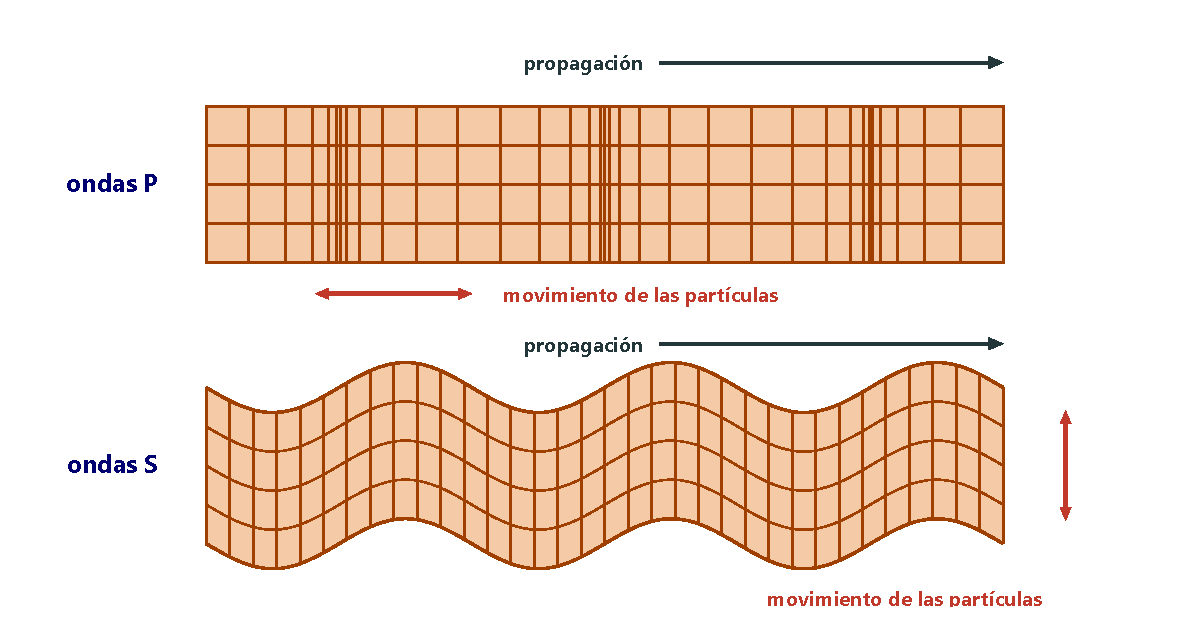
\includegraphics[width=0.7\textwidth]{images/UD13/ondas_sismicas}
    \caption{Ondas sísmicas P y S.}
    \label{fig:ondas_sismicas}
\end{figure}

\begin{exercise}
    En un terremoto se producen ondas sísmicas de dos tipos, P y S. Observa la figura~\ref{fig:ondas_sismicas} y clasifícalas en longitudinales y transversales.
    \begin{solu}
        Las ondas P son \textcolor{red}{longitudinales}: las partículas vibran en la misma dirección en que se propaga la onda (compresiones y dilataciones del terreno). Las ondas S son \textcolor{red}{transversales}: las partículas vibran perpendicularmente a la dirección de propagación.
    \end{solu}
\end{exercise}

%========================================================================================
\section{El sonido: una onda mecánica longitudinal}
%========================================================================================

Muchos animales, y también las personas, usamos el sonido para comunicarnos. Las cuerdas vocales o las cuerdas de un instrumento vibran, hacen vibrar el aire que las rodea y esa vibración llega hasta nuestros oídos. ¿Qué tipo de onda es el sonido?

\subsection{El sonido es un movimiento ondulatorio}

Si apoyas la mano sobre un altavoz mientras suena, notarás que su membrana vibra. Esas vibraciones empujan a las moléculas de aire cercanas, que empujan a su vez a las siguientes: por el aire se propagan zonas de mayor presión (\textbf{compresiones}) y de menor presión (\textbf{dilataciones}). El sonido tiene su origen en la \textbf{vibración de los cuerpos} y se \textbf{propaga} a través de un medio material.

\subsection{El sonido es una onda mecánica}

Si colocamos un timbre sonando dentro de una campana de vidrio conectada a una bomba de vacío, al principio se oye perfectamente. A medida que se extrae el aire, el sonido se debilita hasta que casi deja de oírse, aunque vemos que el martillo del timbre sigue golpeando. Si dejamos entrar de nuevo el aire, el sonido vuelve. El sonido \textbf{necesita un medio material} para propagarse: no se propaga en el vacío.

\begin{figure}[H]
    \centering
    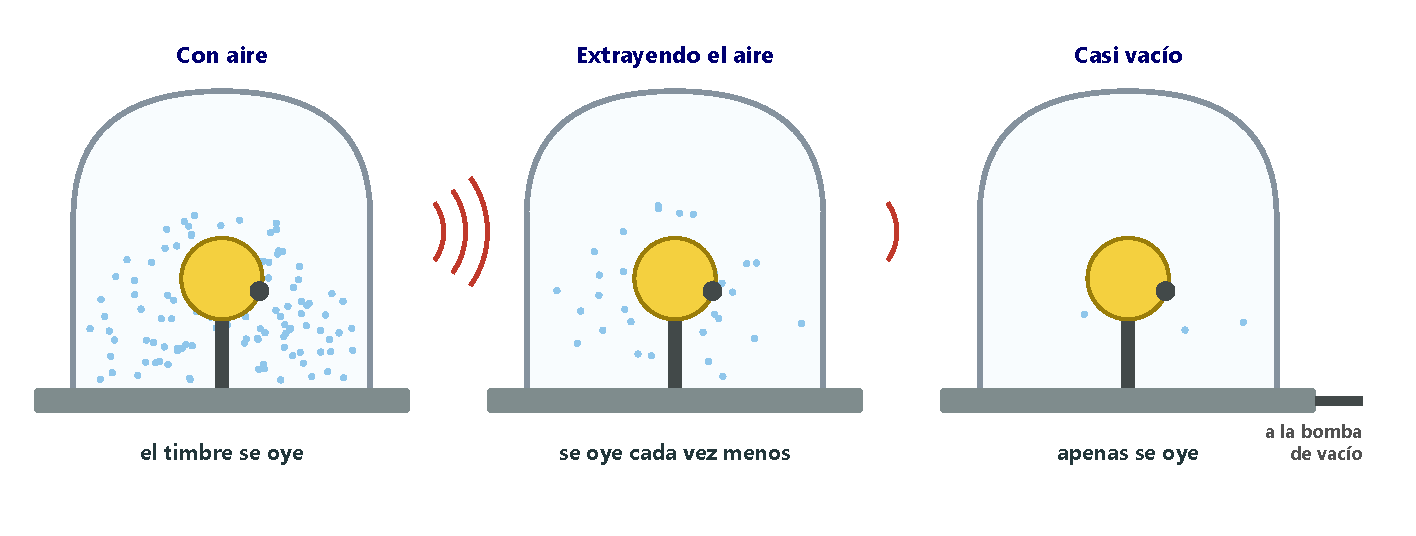
\includegraphics[width=0.85\textwidth]{images/UD13/campana_vacio}
    \caption{Un timbre en una campana de vacío: cuanto menos aire queda, menos se oye.}
    \label{fig:campana_vacio}
\end{figure}

\subsection{El sonido es una onda longitudinal}

Las moléculas de aire vibran hacia delante y hacia atrás en la \textbf{misma dirección} en que avanza el sonido: el sonido es una \textbf{onda longitudinal}. En un medio homogéneo se propaga con velocidad constante, es decir, con movimiento uniforme.

\begin{figure}[H]
    \centering
    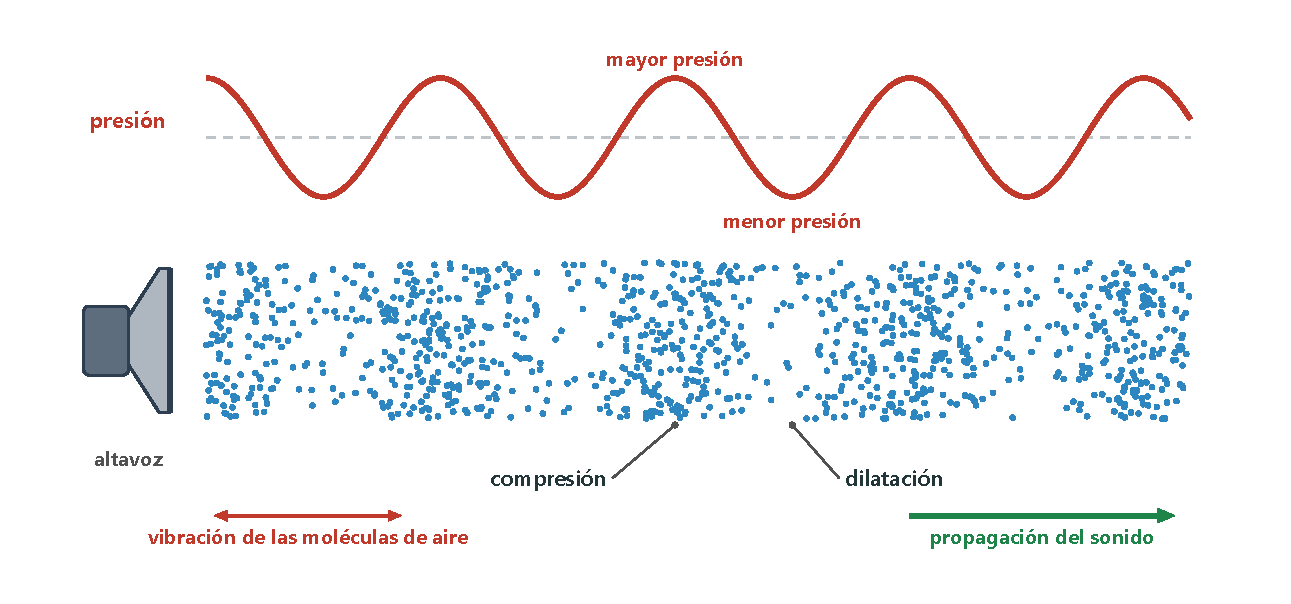
\includegraphics[width=0.9\textwidth]{images/UD13/sonido_compresiones}
    \caption{La membrana del altavoz produce compresiones y dilataciones del aire que se propagan en la misma dirección en que vibran las moléculas.}
    \label{fig:sonido_compresiones}
\end{figure}

La velocidad del sonido depende del medio: en general, es mayor en los sólidos que en los líquidos, y mayor en los líquidos que en los gases. En el aire, a unos \qty{15}{\degreeCelsius}, vale unos \qty{340}{\m\per\s}, y aumenta con la temperatura.

\begin{center}
    % --- tabla antigua ---
    % \begin{tblr}{colspec={lcccccccc}, hlines, vlines, row{1}={bg=ocre!85, fg=white, font=\bfseries}, column{1}={bg=ocre!85, fg=white, font=\bfseries}, cells={font=\small}}
        % Medio & vacío & aire & \ch{O2} & \ch{CO2} & agua & agua de mar & hierro & vidrio \\
        % \(v\) (\unit{\m\per\s}) & -- & 340 & 316 & 258 & 1450 & 1531 & 5100 & 5500 \\
    % \end{tblr}
    % --- tabla nueva ---
    {\small
    \begin{tabular}{@{}lcccccccc@{}}
        \toprule
        \textbf{Medio} & \textbf{vacío} & \textbf{aire} & \textbf{\ch{O2}} & \textbf{\ch{CO2}} & \textbf{agua} & \textbf{agua de mar} & \textbf{hierro} & \textbf{vidrio} \\
        \midrule
        \textbf{\(v\) (\unit{\m\per\s})} & -- & 340 & 316 & 258 & 1450 & 1531 & 5100 & 5500 \\
        \bottomrule
    \end{tabular}
    }
\end{center}

\begin{exercise}
    Observa la tabla anterior y compara la velocidad del sonido en los sólidos, los líquidos y los gases. ¿Por qué no aparece ningún valor en el vacío?
    \begin{solu}
        El sonido es \textcolor{red}{más rápido en los sólidos} (hierro y vidrio, más de \qty{5000}{\m\per\s}) que en los \textcolor{red}{líquidos} (agua, unos \qty{1500}{\m\per\s}), y en estos más que en los \textcolor{red}{gases} (aire, \ch{O2} y \ch{CO2}, unos \qty{300}{\m\per\s}). En el vacío \textcolor{red}{no se propaga}, porque es una onda mecánica.
    \end{solu}
\end{exercise}

\begin{exercise}
    Los ultrasonidos transportan mucha energía y pueden concentrarse en haces muy estrechos. Busca información sobre sus aplicaciones y prepara una breve presentación.
    \begin{solu}
        Respuesta libre. Por ejemplo: \textcolor{red}{ecografías} (seguimiento del embarazo, imágenes del corazón, hígado, riñones, tiroides\ldots), \textcolor{red}{sónar} para medir la profundidad del mar y localizar bancos de peces o submarinos, eliminación de cálculos renales, limpieza de piezas y joyas, detección de grietas en metales o ahuyentadores de animales.
    \end{solu}
\end{exercise}

\begin{example}
    Durante una tormenta vemos un relámpago y oímos el trueno \qty{3}{\s} después. ¿A qué distancia ha caído el rayo?

    La luz llega prácticamente al instante, así que el retraso se debe al sonido:
    \[ d = v \cdot t = \qty{340}{\m\per\s} \cdot \qty{3}{\s} = \textcolor{red}{\qty{1020}{\m}} \approx \qty{1}{\km} \]
\end{example}

\subsection{Intensidad física y nivel de intensidad sonora}

Como todas las ondas, el sonido transporta energía. Su \textbf{intensidad física}, \(I\), es la potencia que atraviesa cada unidad de superficie y, como hemos visto, a una distancia \(r\) de un foco que emite en todas las direcciones vale \(I = P/(4\pi r^2)\): \textbf{disminuye con el cuadrado de la distancia} al foco.

Sin embargo, nuestro oído no percibe la intensidad de forma proporcional. Por eso se usa el \textbf{nivel de intensidad sonora}, que se mide en \textbf{decibelios} (\unit{\decibel}):
\begin{itemize}
    \item El valor \qty{0}{\decibel} corresponde al \textbf{umbral de audición}, la intensidad mínima que puede percibir el oído humano.
    \item Cada vez que la intensidad física se hace \textbf{10 veces mayor}, el nivel de intensidad sonora \textbf{aumenta \qty{10}{\decibel}}. Si la intensidad se multiplica por 100, el nivel sube \qty{20}{\decibel}; si se multiplica por 1000, sube \qty{30}{\decibel}.
    \item El nivel máximo que el oído puede tolerar sin dolor es el \textbf{umbral del dolor}, de unos \qty{120}{\decibel}.
\end{itemize}

\begin{figure}[H]
    \centering
    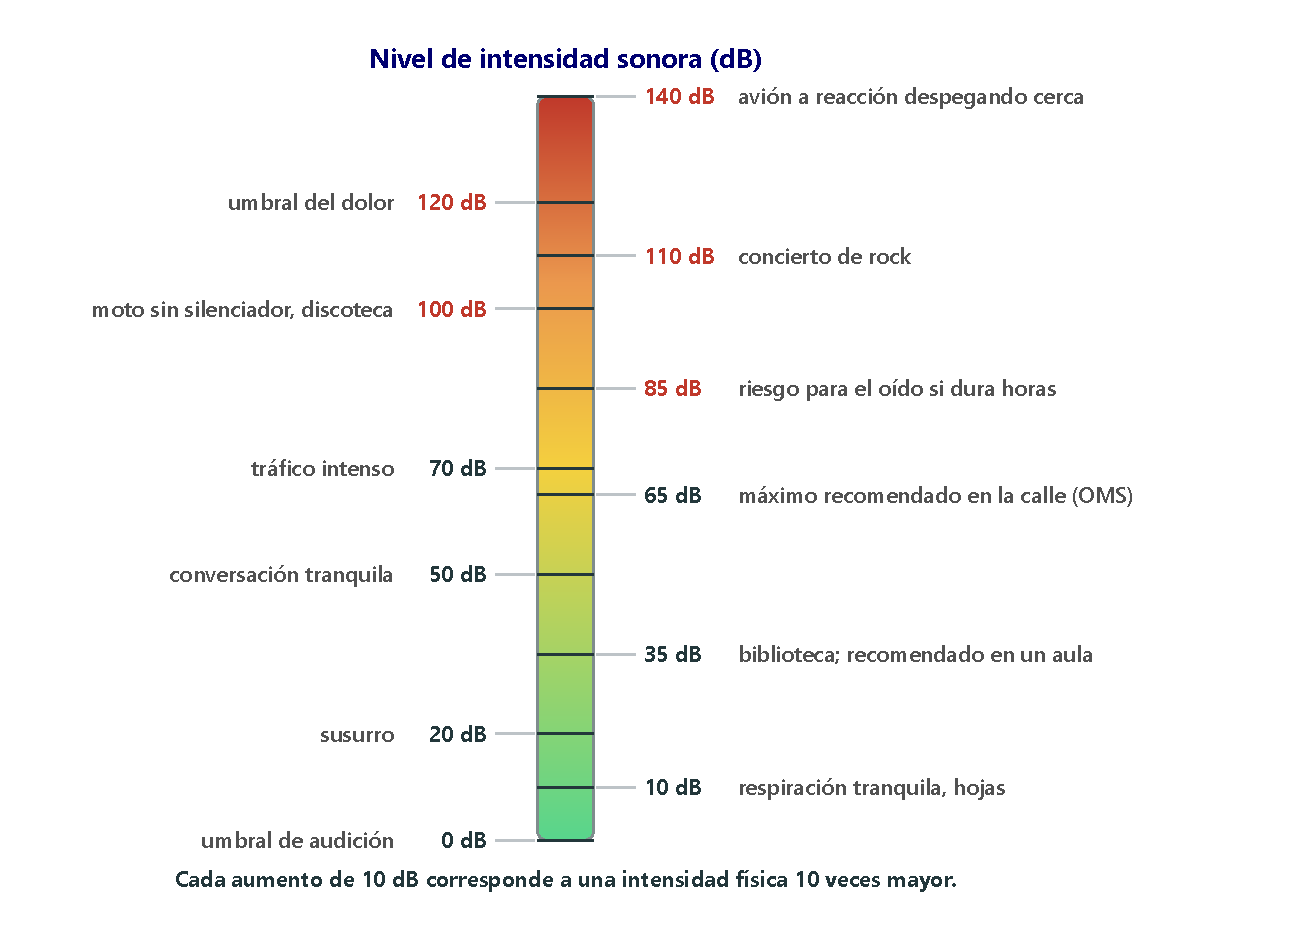
\includegraphics[width=0.95\textwidth]{images/UD13/escala_decibelios}
    \caption{Niveles de intensidad sonora de algunos sonidos habituales.}
    \label{fig:escala_decibelios}
\end{figure}

\begin{remark}
    Exponerse durante mucho tiempo a niveles superiores a unos \qty{85}{\decibel} (auriculares con el volumen alto, discotecas, conciertos) puede dañar el oído de forma permanente.
\end{remark}

\begin{example}
    Una conversación tiene un nivel de \qty{60}{\decibel}. ¿Qué nivel tendrá un sonido cuya intensidad física sea 1000 veces mayor?

    \(1000 = 10 \cdot 10 \cdot 10\): la intensidad se multiplica tres veces por 10, así que el nivel aumenta \(3 \cdot \qty{10}{\decibel}\):
    \[ \qty{60}{\decibel} + \qty{30}{\decibel} = \textcolor{red}{\qty{90}{\decibel}} \]
\end{example}

\subsection{¿Cómo se refleja el sonido? El eco}

Cuando las ondas sonoras encuentran un obstáculo, \textbf{se reflejan}. Si el sonido reflejado nos llega bastante después que el emitido, lo oímos como un sonido distinto: es el \textbf{eco}. Nuestro oído distingue dos sonidos si le llegan separados al menos \qty{0.1}{\s}. En ese tiempo el sonido recorre en el aire \(\qty{340}{\m\per\s} \cdot \qty{0.1}{\s} = \qty{34}{\m}\) de ida y vuelta, así que para percibir eco el obstáculo debe estar, como mínimo, a \textbf{\qty{17}{\m}}. Si está más cerca, el sonido reflejado se superpone al original y lo prolonga: es la \textbf{reverberación}.

El \textbf{sónar} de los barcos usa el eco de los ultrasonidos para medir la profundidad del mar: si el eco tarda un tiempo \(t\), el sonido ha recorrido dos veces la profundidad, \(2d = v \cdot t\).

\begin{figure}[H]
    \centering
    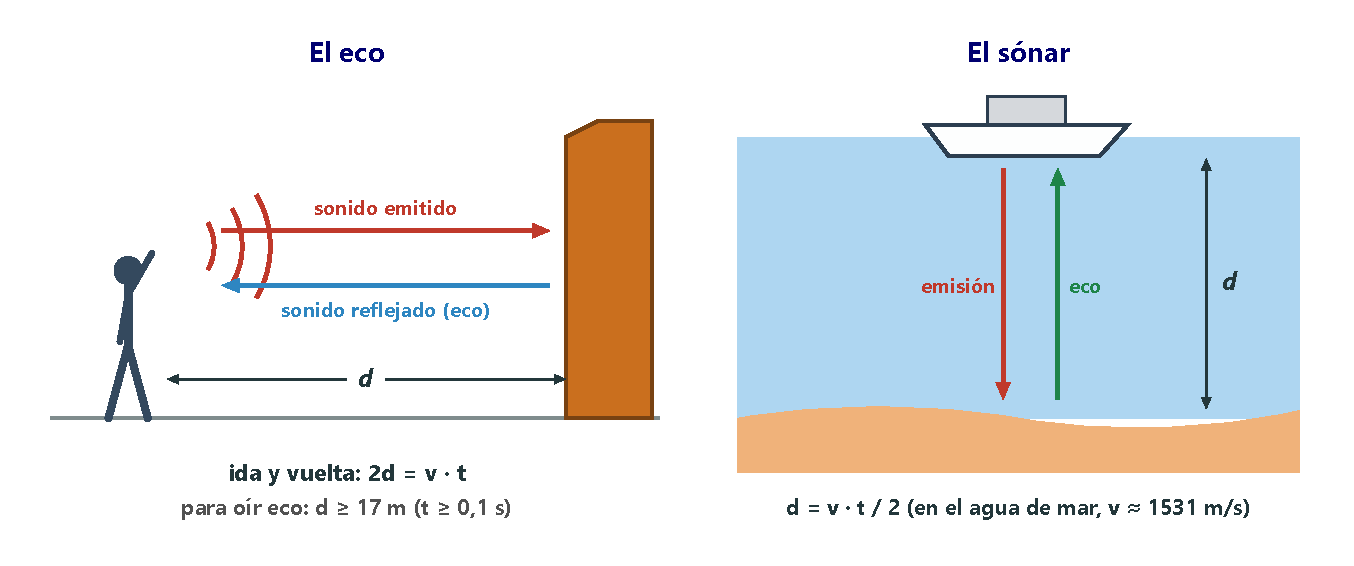
\includegraphics[width=0.95\textwidth]{images/UD13/eco_sonar}
    \caption{El eco y el sónar: el sonido recorre dos veces la distancia hasta el obstáculo.}
    \label{fig:eco_sonar}
\end{figure}

\begin{example}
    Gritamos frente a una pared rocosa y oímos el eco \qty{0.4}{\s} después. ¿A qué distancia está la pared?
    \[ 2d = v \cdot t \quad\Rightarrow\quad d = \frac{\qty{340}{\m\per\s} \cdot \qty{0.4}{\s}}{2} = \textcolor{red}{\qty{68}{\m}} \]
\end{example}

\subsection{¿Cómo se refracta el sonido?}

El sonido se refracta al pasar de un medio a otro y también al pasar de unas capas de aire a otras con distinta temperatura, porque en ellas se propaga con distinta velocidad. Por ejemplo, de noche el aire junto al mar está más frío que el de arriba; el sonido se curva hacia el agua y por eso, a veces, se oyen sonidos de la costa desde barcos muy alejados.

\subsection{¿Cuáles son las cualidades del sonido?}

\begin{itemize}
    \item \textbf{Intensidad}: permite distinguir los sonidos \textbf{fuertes} de los \textbf{débiles}. Depende de la \textbf{amplitud} de la onda: a mayor amplitud, sonido más fuerte.
    \item \textbf{Tono}: permite distinguir los sonidos \textbf{agudos} de los \textbf{graves}. Depende de la \textbf{frecuencia}: los sonidos agudos tienen \textbf{mayor} frecuencia que los graves. El oído humano solo percibe frecuencias entre \qty{20}{\hertz} y \qty{20000}{\hertz}; por debajo están los \textbf{infrasonidos} y por encima, los \textbf{ultrasonidos}.
    \item \textbf{Timbre}: permite distinguir dos sonidos de la misma intensidad y el mismo tono emitidos por focos distintos (por ejemplo, la misma nota tocada por una flauta y por un violín). Depende de la \textbf{forma de la onda}.
\end{itemize}

\begin{figure}[H]
    \centering
    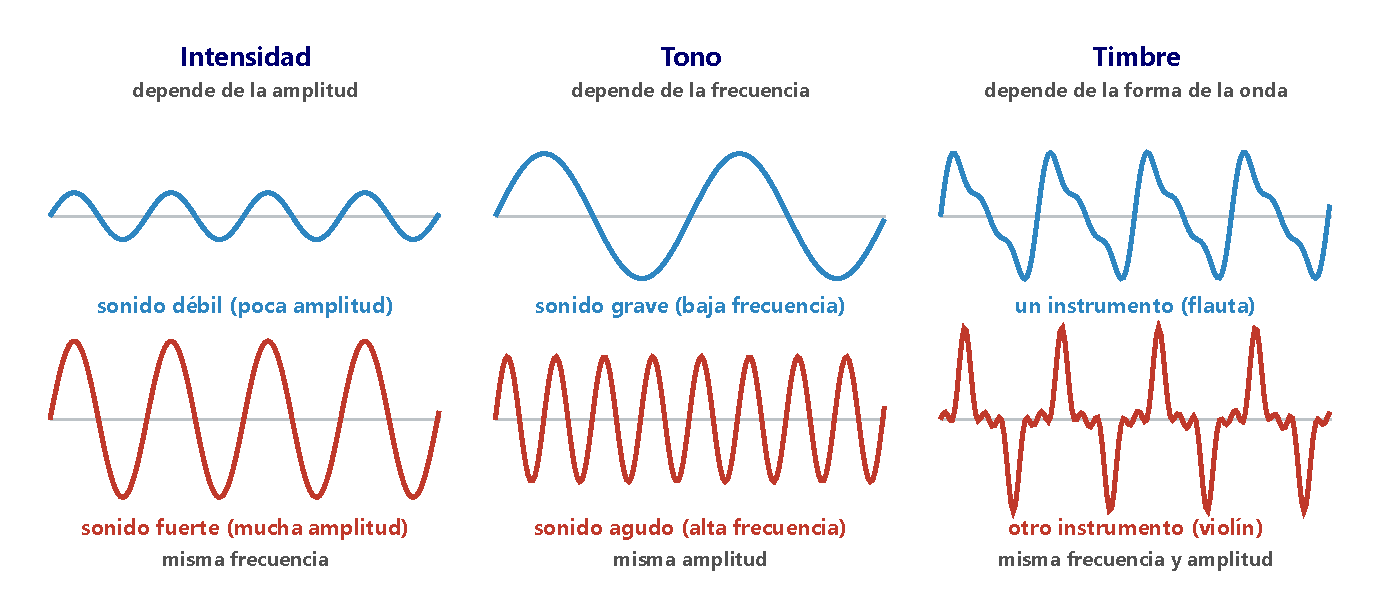
\includegraphics[width=\textwidth]{images/UD13/cualidades_sonido}
    \caption{Las cualidades del sonido dependen de la amplitud (intensidad), de la frecuencia (tono) y de la forma de la onda (timbre).}
    \label{fig:cualidades_sonido}
\end{figure}

\begin{exercise}
    Calcula entre qué valores está la longitud de onda de los sonidos audibles por las personas en el aire.
    \begin{solu}
        \(\lambda = v/f\). Para \qty{20}{\hertz}: \(\lambda = 340/20 = \textcolor{red}{\qty{17}{\m}}\). Para \qty{20000}{\hertz}: \(\lambda = 340/\num{20000} = \textcolor{red}{\qty{0.017}{\m}} = \qty{1.7}{\cm}\).
    \end{solu}
\end{exercise}

%----------------------------------------------------------------------------------------
\subsection*{Actividades de consolidación: el sonido}
%----------------------------------------------------------------------------------------

\begin{exercise}
    La velocidad del sonido en el aire aumenta con la temperatura, como muestra la tabla:
    \begin{center}
        % --- tabla antigua ---
        % \begin{tblr}{colspec={lcccccc}, hlines, vlines, column{1}={bg=ocre!85, fg=white, font=\bfseries}}
            % \(T\) (\unit{\degreeCelsius}) & \(-15\) & \(-10\) & \(-5\) & 0 & 5 & 10 \\
            % \(v\) (\unit{\m\per\s}) & 322 & 325 & 328 & 331 & 334 & 337 \\
        % \end{tblr}
        % --- tabla nueva ---
        \begin{tabular}{@{}lcccccc@{}}
            \toprule
            \textbf{\(T\) (\unit{\degreeCelsius})} & \(-15\) & \(-10\) & \(-5\) & 0 & 5 & 10 \\[3pt]
            \textbf{\(v\) (\unit{\m\per\s})} & 322 & 325 & 328 & 331 & 334 & 337 \\
            \bottomrule
        \end{tabular}
    \end{center}
    \begin{enumerate}[label=\alph*)]
        \item Representa la gráfica velocidad-temperatura. ¿Qué relación hay entre ambas magnitudes?
        \item ¿Qué le ocurrirá a un rayo sonoro que pasa de una zona de aire frío a otra más caliente?
        \item ¿Y si pasa de una zona caliente a otra más fría?
    \end{enumerate}
    \begin{solu}
        a) Los puntos están sobre una \textcolor{red}{recta}: la velocidad aumenta \qty{3}{\m\per\s} por cada \qty{5}{\degreeCelsius} (\qty{0.6}{\m\per\s} por grado). No es una proporcionalidad directa, porque a \qty{0}{\degreeCelsius} la velocidad no es cero.
        \begin{center}
            \begin{tikzpicture}
                \begin{axis}[grafica, xlabel={\(T\) (\unit{\degreeCelsius})}, ylabel={\(v\) (\unit{\m\per\s})}, xmin=-20, xmax=15, ymin=318, ymax=340]
                    \addplot coordinates {(-15,322) (-10,325) (-5,328) (0,331) (5,334) (10,337)};
                \end{axis}
            \end{tikzpicture}
        \end{center}
        b) Pasa a un medio en el que va más deprisa: el rayo \textcolor{red}{se aleja de la normal}.
        c) Pasa a un medio en el que va más despacio: el rayo \textcolor{red}{se acerca a la normal}.
    \end{solu}
\end{exercise}

\begin{exercise}
    Una soprano canta una nota de \qty{1300}{\hertz}. ¿Cuál es la longitud de onda de ese sonido en el aire si se propaga a \qty{332}{\m\per\s}?
    \begin{solu}
        \(\lambda = \dfrac{v}{f} = \dfrac{332}{1300} = \textcolor{red}{\qty{0.255}{\m}}\).
    \end{solu}
\end{exercise}

\begin{exercise}
    Una jueza de atletismo dispara la pistola de salida y oye el eco en una montaña \qty{2.5}{\s} después. ¿A qué distancia está la montaña? Dato: \(v_{\text{sonido}} = \qty{332}{\m\per\s}\).
    \begin{solu}
        El sonido va y vuelve: \(d = \dfrac{v \cdot t}{2} = \dfrac{332 \cdot \num{2.5}}{2} = \textcolor{red}{\qty{415}{\m}}\).
    \end{solu}
\end{exercise}

\begin{exercise}
    Una onda sonora pasa del aire al agua formando cierto ángulo con la normal. ¿Se acercará o se alejará de la normal? Justifícalo.
    \begin{solu}
        \textcolor{red}{Se alejará de la normal}, porque el sonido se propaga más deprisa en el agua (unos \qty{1450}{\m\per\s}) que en el aire (\qty{340}{\m\per\s}). (Al revés que la luz, que es más lenta en el agua.)
    \end{solu}
\end{exercise}

\begin{exercise}
    ¿Podríamos oír desde la Tierra el choque de un meteorito gigante contra la Luna? Razónalo.
    \begin{solu}
        \textcolor{red}{No}: entre la Luna y la Tierra el espacio está prácticamente vacío y el sonido, al ser una onda mecánica, no se propaga en el vacío. Sí podríamos \emph{ver} el destello, porque la luz se propaga en el vacío.
    \end{solu}
\end{exercise}

\begin{exercise}
    El sónar de un barco emite un pulso de ultrasonidos y recibe el eco del fondo \qty{0.52}{\s} después. ¿A qué profundidad está el fondo? Dato: \(v = \qty{1531}{\m\per\s}\).
    \begin{solu}
        \(d = \dfrac{v \cdot t}{2} = \dfrac{1531 \cdot \num{0.52}}{2} = 1531 \cdot \num{0.26} = \textcolor{red}{\qty{398}{\m}}\).
    \end{solu}
\end{exercise}

\begin{exercise}
    Estas dos gráficas representan dos sonidos de la misma frecuencia. ¿Cuál corresponde a un sonido fuerte y cuál a uno débil?
    \begin{center}
        \begin{tikzpicture}
            \begin{axis}[grafica, width=6.5cm, height=4cm, title={\small Sonido A}, xtick=\empty, ytick=\empty, xmin=0, xmax=3, ymin=-2.2, ymax=2.2, xlabel={tiempo}]
                \addplot[mark=none, samples=150, domain=0:3, blue!70!black] {0.5*sin(deg(2*pi*x))};
            \end{axis}
        \end{tikzpicture}\qquad
        \begin{tikzpicture}
            \begin{axis}[grafica, width=6.5cm, height=4cm, title={\small Sonido B}, xtick=\empty, ytick=\empty, xmin=0, xmax=3, ymin=-2.2, ymax=2.2, xlabel={tiempo}]
                \addplot[mark=none, samples=150, domain=0:3] {1.8*sin(deg(2*pi*x))};
            \end{axis}
        \end{tikzpicture}
    \end{center}
    \begin{solu}
        La intensidad depende de la amplitud: el sonido A, de poca amplitud, es \textcolor{red}{débil}, y el sonido B, de gran amplitud, es \textcolor{red}{fuerte}. Como tienen la misma frecuencia, tienen el mismo tono.
    \end{solu}
\end{exercise}

\begin{exercise}
    Un buque oceanográfico envía una señal de sónar hacia el fondo y la recibe \qty{0.1}{\s} después. ¿A qué profundidad está el fondo? Dato: \(v = \qty{1531}{\m\per\s}\).
    \begin{solu}
        \(d = \dfrac{1531 \cdot \num{0.1}}{2} = \textcolor{red}{\qty{76.6}{\m}}\).
    \end{solu}
\end{exercise}

\begin{exercise}
    Lee el texto y responde:
    \begin{marker}
        \emph{¿Por qué oímos a una soprano a pesar de la potencia de toda la orquesta? Al hablar y al cantar, producimos sonidos haciendo vibrar las cuerdas vocales: entre unos \qty{100}{\hertz} y \qty{220}{\hertz} en el habla normal, y entre \qty{50}{\hertz} y \qty{1500}{\hertz} en el canto. Una orquesta suena con más fuerza alrededor de los \qty{500}{\hertz}, y su sonido se debilita a frecuencias más altas. El oído humano es más sensible entre \qty{3000}{\hertz} y \qty{4000}{\hertz}, y muchas cantantes de ópera refuerzan su voz por encima de los \qty{2000}{\hertz}.}
    \end{marker}
    \begin{enumerate}[label=\alph*)]
        \item ¿Son audibles todas las frecuencias que aparecen en el texto?
        \item ¿A qué frecuencia suena con más fuerza una orquesta? ¿Para qué frecuencias es más sensible el oído?
        \item Calcula las longitudes de onda del habla normal y del canto (\(v = \qty{340}{\m\per\s}\)).
        \item ¿Por qué destaca la voz de la soprano sobre la orquesta?
    \end{enumerate}
    \begin{solu}
        a) \textcolor{red}{Sí}: todas están entre \qty{20}{\hertz} y \qty{20000}{\hertz}.
        b) La orquesta alcanza su máximo hacia los \textcolor{red}{\qty{500}{\hertz}}; el oído es más sensible entre \textcolor{red}{\qty{3000}{\hertz} y \qty{4000}{\hertz}}.
        c) Habla: \(\lambda = 340/100 = \qty{3.4}{\m}\) y \(\lambda = 340/220 = \qty{1.55}{\m}\), es decir, \textcolor{red}{entre \qty{1.55}{\m} y \qty{3.4}{\m}}. Canto: \(340/50 = \qty{6.8}{\m}\) y \(340/1500 = \qty{0.23}{\m}\), \textcolor{red}{entre \qty{0.23}{\m} y \qty{6.8}{\m}}.
        d) Porque la soprano concentra potencia en frecuencias \textcolor{red}{superiores a \qty{2000}{\hertz}}, donde la orquesta suena débil y donde el oído es más sensible.
    \end{solu}
\end{exercise}

\begin{exercise}
    Investiga cómo cambian los umbrales de audición y del dolor con la frecuencia:
    \begin{enumerate}[label=\alph*)]
        \item ¿Cuál es, aproximadamente, el umbral de audición para un sonido de \qty{512}{\hertz}?
        \item ¿Y el umbral del dolor para un sonido de \qty{4096}{\hertz}?
    \end{enumerate}
    \begin{solu}
        a) El umbral de audición depende mucho de la frecuencia (es más alto para los sonidos muy graves y muy agudos). A \qty{512}{\hertz} está en \textcolor{red}{unos pocos decibelios, menos de \qty{10}{\decibel}}.
        b) El umbral del dolor varía poco con la frecuencia: unos \textcolor{red}{\qty{120}{\decibel}}.
    \end{solu}
\end{exercise}

\begin{exercise}
    Un sonido tiene un nivel de intensidad de \qty{80}{\decibel}. ¿Qué nivel tendrá si su intensidad física se hace diez veces mayor? ¿Y cien veces mayor?
    \begin{solu}
        Diez veces mayor: \(80 + 10 = \textcolor{red}{\qty{90}{\decibel}}\). Cien veces mayor: \(80 + 20 = \textcolor{red}{\qty{100}{\decibel}}\).
    \end{solu}
\end{exercise}

\begin{exercise}
    Un avión emite un sonido con una potencia de \qty{3000}{\watt}. Calcula la intensidad física con la que se percibe: a) a \qty{1}{\km} del foco; b) a \qty{10}{\km} del foco.
    \begin{solu}
        a) \(I = \dfrac{P}{4\pi r^2} = \dfrac{3000}{4\pi \cdot (\num{1000})^2} = \textcolor{red}{\qty{2.39e-4}{\watt\per\square\m}}\).
        b) A una distancia 10 veces mayor, la intensidad es \(10^2 = 100\) veces menor: \(I = \textcolor{red}{\qty{2.39e-6}{\watt\per\square\m}}\).
    \end{solu}
\end{exercise}

%========================================================================================
\section{La luz: una onda transversal}
%========================================================================================

La luz es una \textbf{onda electromagnética}: se propaga en todas las direcciones desde un foco luminoso sin necesidad de un medio material. Por eso nos llega la luz del Sol y de las estrellas a través del espacio, que está prácticamente vacío. Todas las ondas electromagnéticas son \textbf{transversales}.

La luz se propaga en \textbf{línea recta} en un medio homogéneo; por eso los objetos opacos producen \textbf{sombras}. Su velocidad en el vacío es la mayor que existe:
\[ c = \qty{3e8}{\m\per\s} = \qty{300000}{\km\per\s} \]
En cualquier otro medio, la luz se propaga siempre más despacio.

\begin{example}
    La distancia media entre el Sol y la Tierra es de \qty{1.5e11}{\m}. ¿Cuánto tarda en llegarnos la luz del Sol?
    \[ t = \frac{d}{c} = \frac{\qty{1.5e11}{\m}}{\qty{3e8}{\m\per\s}} = \qty{500}{\s} = \textcolor{red}{\text{8 min 20 s}} \]
    Cuando miramos el Sol, lo vemos como era hace algo más de ocho minutos.
\end{example}

\subsection{¿Cómo se produce la reflexión de la luz?}

La \textbf{reflexión de la luz} es el cambio de dirección que experimenta un rayo luminoso al chocar con una superficie, por ejemplo un espejo, sin atravesarla. La luz reflejada sigue en el mismo medio y cumple las leyes de la reflexión que ya conocemos.

Un \textbf{espejo plano} es una superficie plana, lisa y pulida, que refleja en una sola dirección un haz de rayos paralelos. Para encontrar la imagen de un punto \(P\) de un objeto, trazamos dos rayos que salen de \(P\) y se reflejan en el espejo. Los rayos reflejados se separan, pero sus \textbf{prolongaciones} (hacia detrás del espejo) se cortan en un punto \(P'\): es la imagen de \(P\).

\begin{figure}[H]
    \centering
    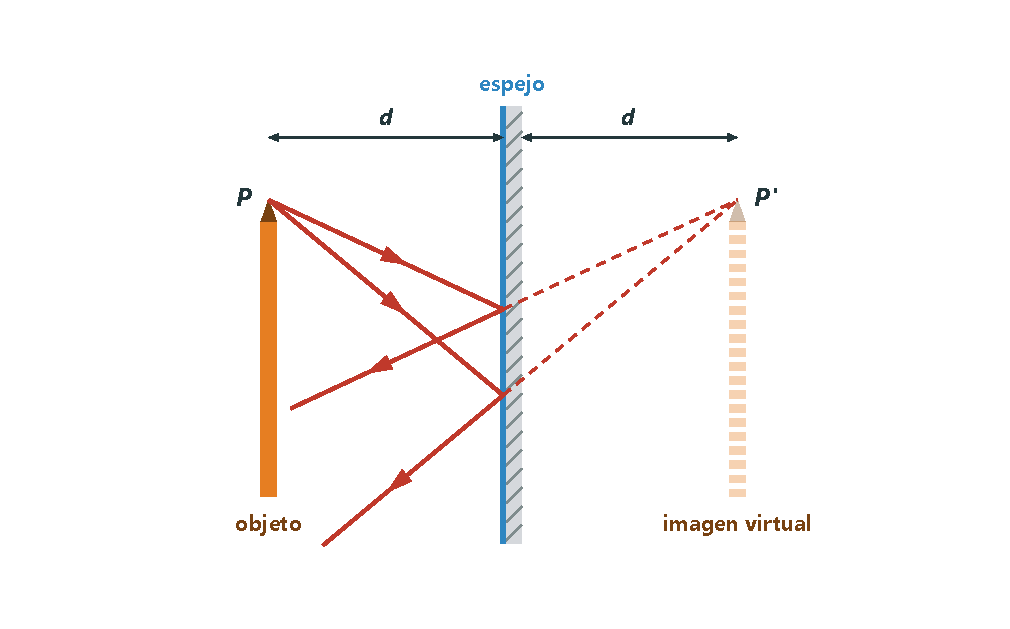
\includegraphics[width=0.65\textwidth]{images/UD13/espejo_plano}
    \caption{Formación de la imagen en un espejo plano: las prolongaciones de los rayos reflejados se cortan detrás del espejo.}
    \label{fig:espejo_plano}
\end{figure}

\begin{marker}
    La imagen en un espejo plano es \textbf{virtual} (se forma con las prolongaciones de los rayos, no con los rayos mismos, y no se puede recoger en una pantalla), \textbf{del mismo tamaño} que el objeto, \textbf{derecha}, está \textbf{a la misma distancia} del espejo que el objeto y tiene \textbf{invertidos la izquierda y la derecha}.
\end{marker}

\subsection{¿Cómo se produce la refracción de la luz?}

La \textbf{refracción de la luz} es el cambio de velocidad, y en general de dirección, que experimenta un rayo de luz al pasar de un medio a otro en el que se propaga con distinta velocidad.

\begin{definition}[Índice de refracción]
    El \textbf{índice de refracción}, \(n\), de un medio es el cociente entre la velocidad de la luz en el vacío, \(c\), y su velocidad en ese medio, \(v\):
    \[ n = \frac{c}{v} \]
    No tiene unidades, porque es el cociente de dos velocidades. Como la luz nunca es más rápida que en el vacío, \(n \geq 1\).
\end{definition}

\begin{center}
    % --- tabla antigua ---
    % \begin{tblr}{colspec={lccccccc}, hlines, vlines, row{1}={bg=ocre!85, fg=white, font=\bfseries}, column{1}={bg=ocre!85, fg=white, font=\bfseries}, cells={font=\small}}
        % Medio & vacío & aire & agua & alcohol & cuarzo & vidrio & diamante \\
        % \(n\) & 1 & \num{1.0003} & \num{1.33} & \num{1.36} & \num{1.46} & \num{1.5} & \num{2.42} \\
    % \end{tblr}
    % --- tabla nueva ---
    {\small
    \begin{tabular}{@{}lccccccc@{}}
        \toprule
        \textbf{Medio} & \textbf{vacío} & \textbf{aire} & \textbf{agua} & \textbf{alcohol} & \textbf{cuarzo} & \textbf{vidrio} & \textbf{diamante} \\
        \midrule
        \textbf{\(n\)} & 1 & \num{1.0003} & \num{1.33} & \num{1.36} & \num{1.46} & \num{1.5} & \num{2.42} \\
        \bottomrule
    \end{tabular}
    }
\end{center}

Cuanto mayor es el índice de refracción, más despacio va la luz por ese medio y decimos que el medio es más \textbf{refringente}. Por eso, cuando la luz pasa de un medio a otro de \textbf{mayor} índice (del aire al agua), el rayo \textbf{se acerca a la normal}; y cuando pasa a uno de \textbf{menor} índice (del agua al aire), \textbf{se aleja de la normal}.

La \textbf{ley de Snell} de la refracción establece que el cociente entre el seno del ángulo de incidencia y el del ángulo de refracción es constante, e igual al cociente entre las velocidades de la luz en los dos medios:
\begin{equation*}
    \boxed{\frac{\sen i}{\sen r} = \frac{v_1}{v_2} = \frac{n_2}{n_1}}
\end{equation*}

\begin{figure}[H]
    \centering
    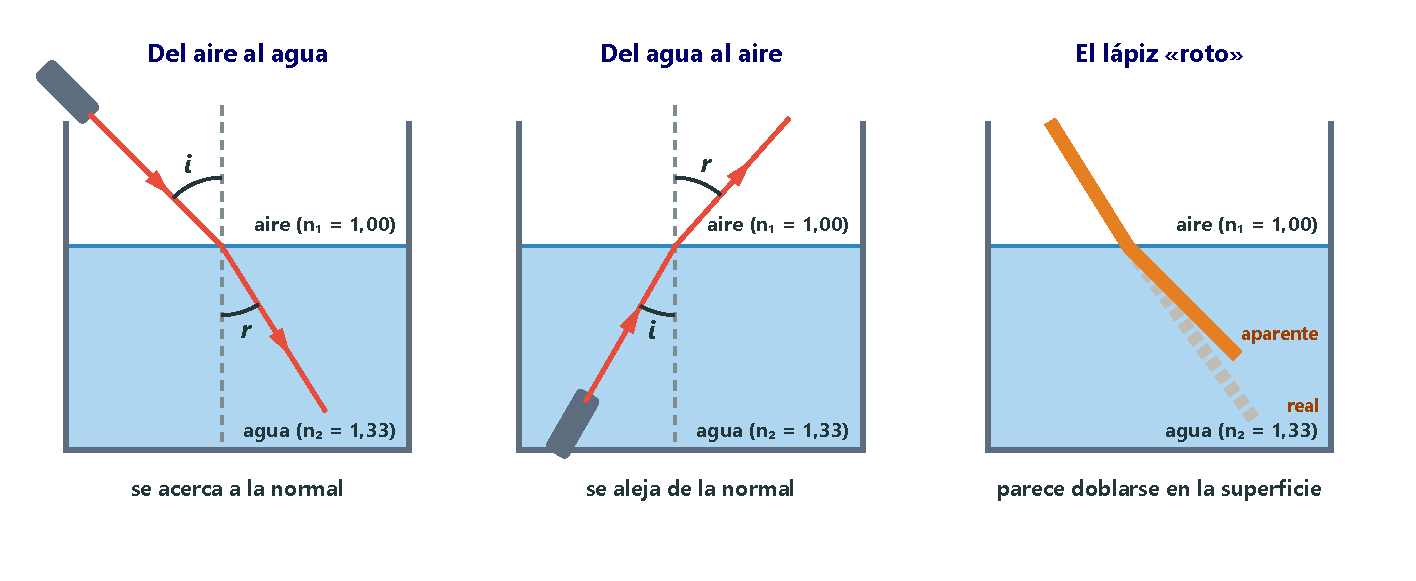
\includegraphics[width=\textwidth]{images/UD13/refraccion_luz}
    \caption{Refracción de un rayo láser al pasar del aire al agua y del agua al aire. La refracción explica que un lápiz parezca doblado al meterlo en agua.}
    \label{fig:refraccion_luz}
\end{figure}

\begin{example}
    Un rayo de luz pasa del aire (\(n_1 = 1\)) al agua (\(n_2 = \num{1.33}\)) con un ángulo de incidencia de \ang{30}. Calcula la velocidad de la luz en el agua y el ángulo de refracción.
    \[ v = \frac{c}{n} = \frac{\qty{3e8}{\m\per\s}}{\num{1.33}} = \textcolor{red}{\qty{2.26e8}{\m\per\s}} \]
    \[ \sen r = \frac{n_1 \cdot \sen i}{n_2} = \frac{1 \cdot \sen \ang{30}}{\num{1.33}} = \frac{\num{0.5}}{\num{1.33}} = \num{0.376} \quad\Rightarrow\quad r = \textcolor{red}{\ang{22.1}} \]
    El rayo se acerca a la normal (\(r < i\)), porque la luz es más lenta en el agua.
\end{example}

\begin{exercise}
    El índice de refracción de un vidrio es \num{1.5}. ¿A qué velocidad se propaga la luz en él?
    \begin{solu}
        \(v = \dfrac{c}{n} = \dfrac{\num{3e8}}{\num{1.5}} = \textcolor{red}{\qty{2e8}{\m\per\s}}\).
    \end{solu}
\end{exercise}

%----------------------------------------------------------------------------------------
\subsection*{Actividades de consolidación: la luz}
%----------------------------------------------------------------------------------------

\begin{exercise}
    Lee el texto y responde:
    \begin{marker}
        \emph{En lo que respecta a la luz, las ondas se parecen a las del sonido: son tridimensionales y tienen una frecuencia, una longitud de onda y una velocidad (en este caso, la de la luz). Pero, sorprendentemente, no necesitan un medio como el aire para propagarse: la luz del Sol y de las estrellas nos llega aunque tenga que atravesar el espacio, que es un vacío casi perfecto. La frecuencia de la luz visible es altísima: cada segundo llegan a nuestros ojos unos 600 billones de ondas.} (Adaptado de Carl Sagan.)
    \end{marker}
    \begin{enumerate}[label=\alph*)]
        \item Según el texto, ¿en qué se diferencian las ondas de luz y las de sonido?
        \item Añade otra diferencia entre ambas.
        \item ¿Qué tienen en común?
        \item Calcula la longitud de onda de una luz de 600 billones de hercios.
        \item Si la luz tarda \qty{1.3}{\s} en llegar de la Luna a la Tierra, ¿a qué distancia está la Luna?
    \end{enumerate}
    \begin{solu}
        a) La luz \textcolor{red}{no necesita un medio material} (es una onda electromagnética) y el sonido sí (es una onda mecánica).
        b) La luz es \textcolor{red}{transversal} y el sonido, longitudinal. Además, la luz es muchísimo más rápida.
        c) Las dos son ondas que \textcolor{red}{transportan energía} sin transportar materia, se propagan en las tres dimensiones y tienen frecuencia, longitud de onda y velocidad; las dos se reflejan y se refractan.
        d) \(f = \qty{6e14}{\hertz}\); \(\lambda = \dfrac{c}{f} = \dfrac{\num{3e8}}{\num{6e14}} = \textcolor{red}{\qty{5e-7}{\m}} = \qty{500}{\nano\m}\) (luz verde-azulada).
        e) \(d = c \cdot t = \num{3e8} \cdot \num{1.3} = \textcolor{red}{\qty{3.9e8}{\m}}\), unos \qty{390000}{\km}. (La distancia media real es de unos \qty{384000}{\km}: la luz tarda unos \qty{1.28}{\s}.)
    \end{solu}
\end{exercise}

\begin{exercise}
    Copia el esquema en tu cuaderno e identifica: a) el medio 1 y el medio 2; b) la superficie de separación; c) la normal; d) los ángulos de incidencia, de reflexión y de refracción.
    \begin{center}
        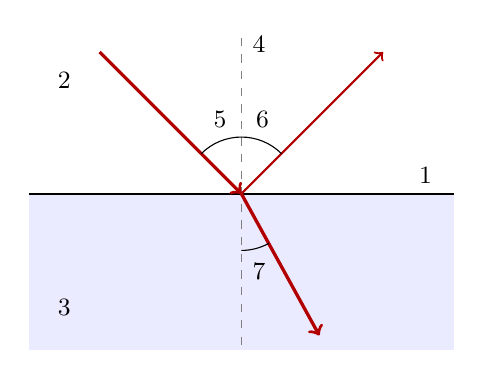
\begin{tikzpicture}[scale=0.9]
            \fill[blue!8] (-3,0) rectangle (3,-2.2);
            \draw[thick] (-3,0) -- (3,0);
            \draw[dashed, gray] (0,2.2) -- (0,-2.2);
            \draw[very thick, red!70!black, ->] (-2,2) -- (0,0);
            \draw[thick, red!70!black, ->] (0,0) -- (2,2);
            \draw[very thick, red!70!black, ->] (0,0) -- (1.1,-2);
            \node[above] at (2.6,0) {\small 1};
            \node at (-2.5,1.6) {\small 2};
            \node at (-2.5,-1.6) {\small 3};
            \node at (0.25,2.1) {\small 4};
            \draw (0,0.8) arc (90:135:0.8); \node at (-0.3,1.05) {\small 5};
            \draw (0,0.8) arc (90:45:0.8); \node at (0.3,1.05) {\small 6};
            \draw (0,-0.8) arc (270:299:0.8); \node at (0.25,-1.1) {\small 7};
        \end{tikzpicture}
    \end{center}
    \begin{solu}
        a) \textcolor{red}{2} es el medio 1 (por donde llega el rayo) y \textcolor{red}{3} es el medio 2. b) La superficie de separación es la línea horizontal (\textcolor{red}{1}). c) La normal es la línea discontinua (\textcolor{red}{4}). d) \textcolor{red}{5} es el ángulo de incidencia, \textcolor{red}{6} el de reflexión (igual que el de incidencia) y \textcolor{red}{7} el de refracción (menor: el medio 2 es más refringente).
    \end{solu}
\end{exercise}

\begin{exercise}
    Con un montaje como el de la figura~\ref{fig:refraccion_luz}, un láser pasa del aire al vidrio. Se han medido estos ángulos:
    \begin{center}
        % --- tabla antigua ---
        % \begin{tblr}{colspec={ccccc}, hlines, vlines, row{1}={bg=ocre!85, fg=white, font=\bfseries}}
            % Incidencia & Refracción & \(\sen i\) & \(\sen r\) & \(\sen i / \sen r\) \\
            % \ang{15} & \ang{9.43} & \num{0.259} & \num{0.164} & \ldots \\
            % \ang{30} & \ang{18.40} & \num{0.500} & \num{0.316} & \ldots \\
            % \ang{45} & \ang{26.60} & \num{0.707} & \num{0.448} & \ldots \\
        % \end{tblr}
        % --- tabla nueva ---
        \begin{tabular}{@{}ccccc@{}}
            \toprule
            \textbf{Incidencia} & \textbf{Refracción} & \textbf{\(\sen i\)} & \textbf{\(\sen r\)} & \textbf{\(\sen i / \sen r\)} \\
            \midrule
            \ang{15} & \ang{9.43} & \num{0.259} & \num{0.164} & \ldots \\[3pt]
            \ang{30} & \ang{18.40} & \num{0.500} & \num{0.316} & \ldots \\[3pt]
            \ang{45} & \ang{26.60} & \num{0.707} & \num{0.448} & \ldots \\
            \bottomrule
        \end{tabular}
    \end{center}
    \begin{enumerate}[label=\alph*)]
        \item Completa la última columna.
        \item ¿Cómo es ese cociente? ¿Qué relación guarda con la velocidad de la luz en los dos medios?
        \item ¿Qué ocurre si el ángulo de incidencia es \ang{0}?
    \end{enumerate}
    \begin{solu}
        a) \(\num{0.259}/\num{0.164} = \num{1.58}\); \(\num{0.500}/\num{0.316} = \num{1.58}\); \(\num{0.707}/\num{0.448} = \num{1.58}\).
        b) Es \textcolor{red}{constante} (\(\approx \num{1.58}\)): es el cociente \(v_{\text{aire}}/v_{\text{vidrio}}\), que coincide con el índice de refracción del vidrio. La luz va \num{1.58} veces más despacio en este vidrio.
        c) El rayo entra en el vidrio \textcolor{red}{sin desviarse}.
    \end{solu}
\end{exercise}

\begin{exercise}
    Repetimos la experiencia anterior sustituyendo el vidrio por agua y obtenemos:
    \begin{center}
        % --- tabla antigua ---
        % \begin{tblr}{colspec={ccccc}, hlines, vlines, row{1}={bg=ocre!85, fg=white, font=\bfseries}}
            % Incidencia & Refracción & \(\sen i\) & \(\sen r\) & \(\sen i / \sen r\) \\
            % \ang{15} & \ang{11.23} & \num{0.259} & \num{0.195} & \ldots \\
            % \ang{30} & \ang{22.00} & \num{0.500} & \num{0.375} & \ldots \\
            % \ang{45} & \ang{32.00} & \num{0.707} & \num{0.530} & \ldots \\
        % \end{tblr}
        % --- tabla nueva ---
        \begin{tabular}{@{}ccccc@{}}
            \toprule
            \textbf{Incidencia} & \textbf{Refracción} & \textbf{\(\sen i\)} & \textbf{\(\sen r\)} & \textbf{\(\sen i / \sen r\)} \\
            \midrule
            \ang{15} & \ang{11.23} & \num{0.259} & \num{0.195} & \ldots \\[3pt]
            \ang{30} & \ang{22.00} & \num{0.500} & \num{0.375} & \ldots \\[3pt]
            \ang{45} & \ang{32.00} & \num{0.707} & \num{0.530} & \ldots \\
            \bottomrule
        \end{tabular}
    \end{center}
    \begin{enumerate}[label=\alph*)]
        \item Completa la última columna.
        \item Compara con la actividad anterior. ¿Qué ley de la refracción puedes enunciar?
        \item Explica por qué una pajita metida en un vaso de agua parece doblada.
    \end{enumerate}
    \begin{solu}
        a) \(\num{1.33}\) en los tres casos (\num{1.328}, \num{1.333} y \num{1.334}).
        b) Para el mismo ángulo de incidencia, los ángulos de refracción son \textcolor{red}{mayores} que en el vidrio: el agua es menos refringente. En los dos casos, \textcolor{red}{el cociente \(\sen i / \sen r\) es constante} para cada par de medios (ley de Snell) e igual al índice de refracción del segundo medio respecto del aire.
        c) La luz que sale de la parte sumergida pasa del agua al aire y \textcolor{red}{se aleja de la normal}. Nuestro cerebro prolonga los rayos en línea recta y «ve» la parte sumergida más arriba de donde está: la pajita parece quebrada en la superficie.
    \end{solu}
\end{exercise}

\begin{exercise}
    En un espejo plano, el rayo incidente y el reflejado forman entre sí un ángulo de \ang{100}. ¿Qué ángulo forma el rayo incidente con la superficie del espejo?
    \begin{solu}
        Cada rayo forma con la normal \(\ang{100}/2 = \ang{50}\). Con la superficie: \(\ang{90} - \ang{50} = \textcolor{red}{\ang{40}}\).
    \end{solu}
\end{exercise}

\begin{exercise}
    Calcula la velocidad de la luz en el agua (\(n = \num{1.33}\)), en el cuarzo (\(n = \num{1.46}\)) y en el diamante (\(n = \num{2.42}\)). Dato: \(c = \qty{3e8}{\m\per\s}\).
    \begin{solu}
        \(v = c/n\): agua, \(\textcolor{red}{\qty{2.26e8}{\m\per\s}}\); cuarzo, \(\textcolor{red}{\qty{2.05e8}{\m\per\s}}\); diamante, \(\textcolor{red}{\qty{1.24e8}{\m\per\s}}\).
    \end{solu}
\end{exercise}

\begin{exercise}
    ¿Puede una sustancia tener un índice de refracción de \num{0.9}? Justifícalo.
    \begin{solu}
        \textcolor{red}{No}: si \(n = c/v = \num{0.9}\), la luz iría por ese medio más deprisa que por el vacío (\(v = c/\num{0.9} \approx \num{1.11}\,c\)), y la velocidad de la luz en el vacío es la máxima posible.
    \end{solu}
\end{exercise}

\begin{exercise}
    ¿Con qué ángulo debe incidir un rayo de luz sobre un espejo para que el rayo incidente y el reflejado sean perpendiculares?
    \begin{solu}
        Entre los dos deben sumar \ang{90} y son iguales: \(i = \textcolor{red}{\ang{45}}\).
    \end{solu}
\end{exercise}

\begin{exercise}
    Un rayo de luz pasa del agua (\(n = \num{1.33}\)) al aire (\(n = 1\)) y el rayo refractado sale rasante, formando \ang{90} con la normal. ¿Cuál era el ángulo de incidencia?
    \begin{solu}
        \(n_1 \sen i = n_2 \sen r \Rightarrow \num{1.33} \cdot \sen i = 1 \cdot \sen \ang{90} = 1\). \(\sen i = \dfrac{1}{\num{1.33}} = \num{0.752}\), \(i = \textcolor{red}{\ang{48.8}}\). (Si el ángulo de incidencia es mayor, la luz no sale del agua: se refleja por completo. Es la \emph{reflexión total}, en la que se basa la fibra óptica.)
    \end{solu}
\end{exercise}

\begin{exercise}
    ¿Por qué no somos capaces de leer un cartel reflejado en un espejo?
    \begin{solu}
        Porque la imagen de un espejo plano tiene \textcolor{red}{invertidas la izquierda y la derecha}: las letras aparecen al revés y el texto se lee de derecha a izquierda. Por eso en las ambulancias se escribe «AMBULANCIA» al revés: así se lee bien en el retrovisor.
    \end{solu}
\end{exercise}

\begin{exercise}
    Escribe tu nombre tal y como se vería reflejado en un espejo y compruébalo.
    \begin{solu}
        Respuesta libre. Hay que escribir las letras de derecha a izquierda y cada una invertida.
    \end{solu}
\end{exercise}

%========================================================================================
\section{El espectro electromagnético}
%========================================================================================

\subsection{La dispersión de la luz blanca}

Un \textbf{prisma óptico} es un cuerpo transparente, homogéneo e isótropo, limitado por caras planas no paralelas, cuyo índice de refracción es mayor que el del aire. Cuando un rayo de luz de un solo color llega a una de sus caras, se refracta acercándose a la normal; al salir por la otra cara, vuelve a refractarse alejándose de ella. En total, el rayo se desvía.

La \textbf{luz blanca} es una mezcla de radiaciones de distintos colores (distintas longitudes de onda). Dentro del vidrio, cada color se propaga con una velocidad ligeramente distinta, así que cada uno se refracta con un ángulo diferente: el violeta es el que más se desvía y el rojo, el que menos. Al salir del prisma, los colores se separan. Este fenómeno se llama \textbf{dispersión} de la luz, y la banda de colores que se obtiene es el \textbf{espectro visible} de la luz blanca. El arcoíris es un ejemplo natural: las gotas de lluvia actúan como pequeños prismas.

\begin{figure}[H]
    \centering
    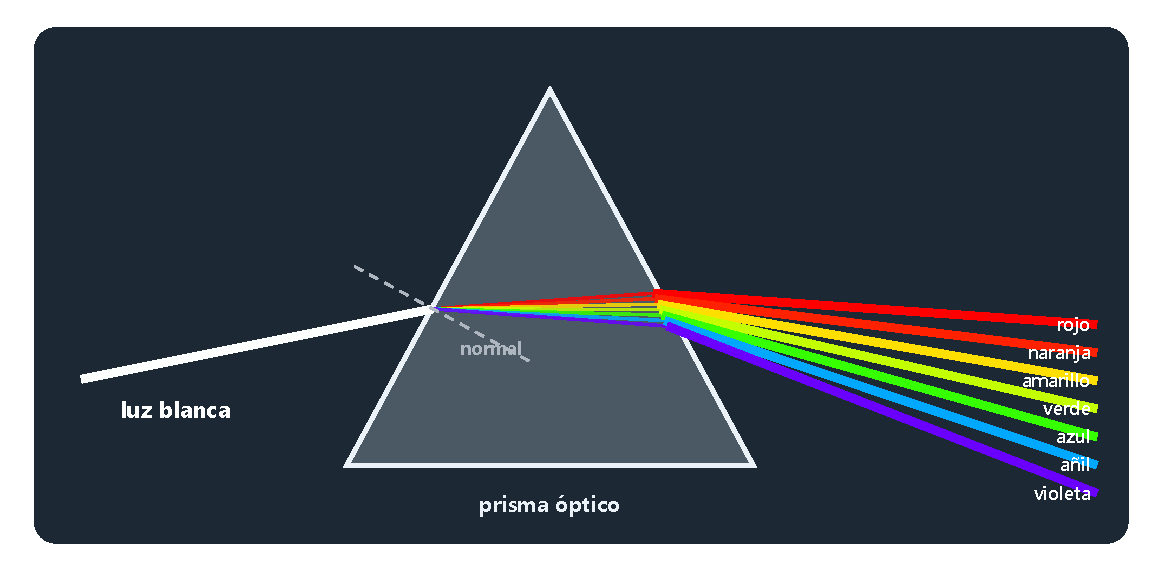
\includegraphics[width=0.75\textwidth]{images/UD13/prisma}
    \caption{Dispersión de la luz blanca en un prisma óptico.}
    \label{fig:prisma}
\end{figure}

\subsection{El espectro electromagnético y sus aplicaciones}

La luz visible es solo una pequeña parte de un conjunto mucho más amplio de ondas, el \textbf{espectro electromagnético}. Todas son ondas electromagnéticas, se propagan en el vacío a \qty{3e8}{\m\per\s} y cumplen \(c = \lambda \cdot f\); se diferencian en su frecuencia y su longitud de onda. Cuanto mayor es la frecuencia, \textbf{mayor es la energía} que transporta la radiación.

\begin{figure}[H]
    \centering
    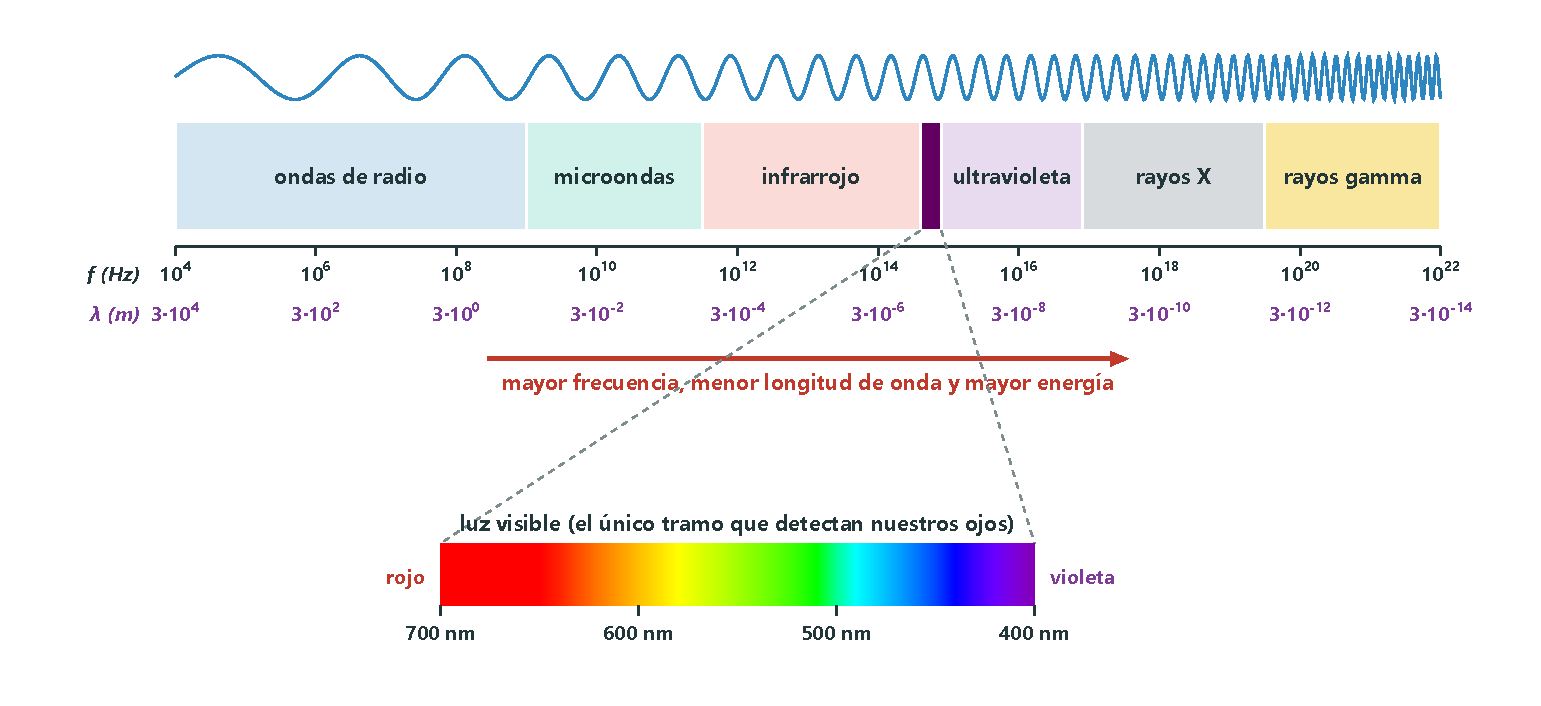
\includegraphics[width=\textwidth]{images/UD13/espectro_em}
    \caption{El espectro electromagnético. La luz visible ocupa un tramo muy estrecho, entre unos \qty{700}{\nano\m} (rojo) y \qty{400}{\nano\m} (violeta).}
    \label{fig:espectro_em}
\end{figure}

\begin{center}
    % --- tabla antigua ---
    % \begin{tblr}{colspec={Q[l,3.2cm]X}, width=\linewidth, hlines, vlines, row{1}={bg=ocre!85, fg=white, font=\bfseries}, column{1}={font=\bfseries}, cells={font=\small}}
        % Radiación & Algunas aplicaciones \\
        % Ondas de radio & Radio y televisión, comunicaciones. Los radiotelescopios captan las ondas de radio que emiten algunas estrellas y galaxias. \\
        % Microondas & Radar (detección de barcos y aviones, control de velocidad), telefonía móvil, wifi, comunicaciones por satélite y hornos de microondas, en los que el agua de los alimentos absorbe la radiación y se calienta. \\
        % Infrarrojos & Los emite cualquier cuerpo caliente (también nuestro cuerpo). Mandos a distancia, cámaras de visión nocturna y termografía, que detecta zonas del cuerpo con una temperatura anormal (inflamaciones, algunos tumores, lesiones deportivas). \\
        % Luz visible & Visión, iluminación, fotosíntesis, láser, fibra óptica. \\
        % Ultravioleta & Broncean y queman la piel, que se oscurece para defenderse. Se usan como desinfectante (esterilización) y para detectar rastros biológicos o billetes y obras de arte falsificados. \\
        % Rayos X & Atraviesan con facilidad los tejidos blandos, pero no los huesos: radiografías y tomografía axial computarizada (TAC), que crea imágenes en 3D de los órganos. \\
        % Rayos gamma & Los emiten las sustancias radiactivas; tienen muchísima energía. Medicina nuclear (gammagrafías, diagnóstico de tumores) y radiocirugía con «bisturí de rayos gamma» para tratar tumores en zonas delicadas. \\
    % \end{tblr}
    % --- tabla nueva ---
    {\small
    \begin{tabular}{@{}L{3.2cm} p{0.78\linewidth}@{}}
        \toprule
        \textbf{Radiación} & \textbf{Algunas aplicaciones} \\
        \midrule
        \textbf{Ondas de radio} & Radio y televisión, comunicaciones. Los radiotelescopios captan las ondas de radio que emiten algunas estrellas y galaxias. \\[3pt]
        \textbf{Microondas} & Radar (detección de barcos y aviones, control de velocidad), telefonía móvil, wifi, comunicaciones por satélite y hornos de microondas, en los que el agua de los alimentos absorbe la radiación y se calienta. \\[3pt]
        \textbf{Infrarrojos} & Los emite cualquier cuerpo caliente (también nuestro cuerpo). Mandos a distancia, cámaras de visión nocturna y termografía, que detecta zonas del cuerpo con una temperatura anormal (inflamaciones, algunos tumores, lesiones deportivas). \\[3pt]
        \textbf{Luz visible} & Visión, iluminación, fotosíntesis, láser, fibra óptica. \\[3pt]
        \textbf{Ultravioleta} & Broncean y queman la piel, que se oscurece para defenderse. Se usan como desinfectante (esterilización) y para detectar rastros biológicos o billetes y obras de arte falsificados. \\[3pt]
        \textbf{Rayos X} & Atraviesan con facilidad los tejidos blandos, pero no los huesos: radiografías y tomografía axial computarizada (TAC), que crea imágenes en 3D de los órganos. \\[3pt]
        \textbf{Rayos gamma} & Los emiten las sustancias radiactivas; tienen muchísima energía. Medicina nuclear (gammagrafías, diagnóstico de tumores) y radiocirugía con «bisturí de rayos gamma» para tratar tumores en zonas delicadas. \\
        \bottomrule
    \end{tabular}
    }
\end{center}

\begin{remark}
    El ultravioleta más energético, los rayos X y los rayos gamma son \textbf{radiaciones ionizantes}: tienen energía suficiente para arrancar electrones de los átomos y dañar las células y el ADN. Por eso su uso médico está muy controlado y el personal que trabaja con ellas se protege.
\end{remark}

\begin{exercise}
    Un horno de microondas funciona con una frecuencia de \qty{2.45}{\giga\hertz}. ¿Cuál es la longitud de onda de su radiación?
    \begin{solu}
        \(\lambda = \dfrac{c}{f} = \dfrac{\num{3e8}}{\num{2.45e9}} = \textcolor{red}{\qty{0.122}{\m}} \approx \qty{12}{\cm}\).
    \end{solu}
\end{exercise}

%----------------------------------------------------------------------------------------
\subsection*{Actividades de consolidación: el espectro electromagnético}
%----------------------------------------------------------------------------------------

\begin{exercise}
    Con ayuda de la figura~\ref{fig:espectro_em}, indica entre qué frecuencias aproximadas se encuentran las microondas y los rayos X. ¿Qué longitudes de onda les corresponden?
    \begin{solu}
        Microondas: \textcolor{red}{entre \qty{1e9}{\hertz} y unos \qty{3e11}{\hertz}}, con \(\lambda = c/f\) entre \qty{0.3}{\m} y \qty{1}{\milli\m}. Rayos X: \textcolor{red}{entre unos \qty{1e17}{\hertz} y \qty{3e19}{\hertz}}, con longitudes de onda entre unos \qty{3e-9}{\m} y \qty{1e-11}{\m}. (Los límites entre zonas no son exactos.)
    \end{solu}
\end{exercise}

\begin{exercise}
    Ordena de mayor a menor frecuencia: rayos gamma, ondas de radio, microondas, ondas de televisión, rayos X, infrarrojos, ultravioleta y luz visible.
    \begin{solu}
        \textcolor{red}{Rayos gamma \(>\) rayos X \(>\) ultravioleta \(>\) luz visible \(>\) infrarrojos \(>\) microondas \(>\) ondas de televisión \(>\) ondas de radio} (las de televisión son ondas de radio de frecuencia más alta). (Los llamados \emph{rayos cósmicos} no son ondas electromagnéticas, sino partículas de muy alta energía; ver la actividad siguiente.)
    \end{solu}
\end{exercise}

\begin{exercise}
    Describe algunas aplicaciones médicas de las radiaciones electromagnéticas.
    \begin{solu}
        Por ejemplo: \textcolor{red}{termografía} infrarroja, \textcolor{red}{desinfección} con ultravioleta, \textcolor{red}{radiografías} y \textcolor{red}{TAC} con rayos X, \textcolor{red}{gammagrafías} y radiocirugía con rayos gamma.
    \end{solu}
\end{exercise}

\begin{exercise}
    Los rayos cósmicos llegan a la Tierra desde el espacio y tienen muchísima energía. La atmósfera nos protege de la mayor parte de ellos.
    \begin{enumerate}[label=\alph*)]
        \item Busca de qué partículas están formados y cómo nos protegen el campo magnético terrestre y la atmósfera.
        \item ¿Pueden estar expuestos a ellos los astronautas y las tripulaciones de los aviones?
    \end{enumerate}
    \begin{solu}
        a) Están formados sobre todo por \textcolor{red}{protones} (alrededor del \qty{90}{\percent}) y \textcolor{red}{núcleos de helio}, además de electrones y núcleos más pesados. Al ser partículas con carga, el \textcolor{red}{campo magnético terrestre desvía} muchas de ellas; las que llegan chocan con los átomos de la \textcolor{red}{atmósfera}, que absorbe la mayor parte de su energía.
        b) \textcolor{red}{Sí}: fuera de la atmósfera, y también a la altura a la que vuelan los aviones, la protección es menor. Por eso se controla la dosis de radiación que reciben los astronautas y las tripulaciones aéreas.
    \end{solu}
\end{exercise}

\begin{exercise}
    El Sol emite, además de luz visible, radiación infrarroja y ultravioleta.
    \begin{enumerate}[label=\alph*)]
        \item Busca información sobre qué partes de la atmósfera absorben cada una de estas radiaciones.
        \item ¿Cómo debemos protegernos de la radiación ultravioleta?
    \end{enumerate}
    \begin{solu}
        a) Parte del \textcolor{red}{infrarrojo} es absorbido por el vapor de agua y el dióxido de carbono; esos gases absorben también el infrarrojo que emite la superficie terrestre y mantienen la temperatura del planeta (\emph{efecto invernadero natural}). La \textcolor{red}{capa de ozono} absorbe la mayor parte del ultravioleta, pero no todo: una parte llega a la superficie.
        b) Evitando el sol en las horas centrales del día, usando \textcolor{red}{cremas con filtro solar}, gorra, ropa y \textcolor{red}{gafas de sol} homologadas, y bebiendo agua. Así se previenen quemaduras, envejecimiento de la piel, cáncer de piel y lesiones en los ojos.
    \end{solu}
\end{exercise}

\begin{exercise}
    Recorta un disco de cartulina blanca, divídelo en seis sectores y píntalos de rojo, naranja, amarillo, verde, azul y violeta. Atraviésalo por el centro con un lápiz y hazlo girar muy deprisa. ¿Qué observas? ¿Qué demuestra?
    \begin{solu}
        Si gira lo bastante rápido (más de unas 100 vueltas por minuto), el ojo no distingue los sectores y el disco parece \textcolor{red}{blanquecino}. Demuestra que la \textcolor{red}{luz blanca es la suma de todos los colores} (es el llamado disco de Newton).
    \end{solu}
\end{exercise}


%----------------------------------------------------------------------------------------
%	ANEXOS: actividades de síntesis, prácticas y situaciones de aprendizaje de todas las unidades
%----------------------------------------------------------------------------------------


    \part{Anexos}

    % Capítulos «Anexo A, B, C» en vez de «Unidad 14, 15, 16» (también en cabeceras y número de los ejercicios)
    \appendix
    \renewcommand{\chaptername}{Anexo}
    \renewcommand{\appendixname}{Anexo}

    \chapterimage{images/portada_cabeceras/cabecera_general}
    \chapter{Actividades de síntesis}

    % Actividades de síntesis de cada unidad (resumen, mapa conceptual y diccionario científico).
% Se incluye en el anexo de Libro_4_ESO_ES.tex. Ordenado por unidades.

%========================================================================================
\section{Unidad 1. El trabajo científico}
%========================================================================================
% (sacado del final de UD1_Trabajo_cientifico.tex)

\begin{enumerate}[label=\numberballred]
    \item \textbf{Resumen.} Elabora un resumen de la unidad respondiendo a estas preguntas:
    \begin{itemize}
        \item ¿Cuáles son las etapas del método científico? ¿Qué diferencia hay entre causalidad y correlación?
        \item ¿Cómo se analizan los resultados de un experimento? ¿Qué diferencia hay entre una ley, una teoría y un modelo?
        \item ¿Qué son las magnitudes? ¿Cuáles son las unidades básicas del SI? ¿Para qué sirve la notación científica?
        \item ¿Qué son las ecuaciones de dimensiones?
        \item ¿Cómo se expresa el resultado de una medida? ¿Cómo se calculan el error absoluto y el relativo?
        \item ¿Qué diferencia hay entre las magnitudes escalares y las vectoriales? ¿Cómo se suman los vectores?
        \item ¿Qué materiales e instrumentos de laboratorio conoces? ¿Qué normas de seguridad hay que seguir?
    \end{itemize}
    \item \textbf{Mapa conceptual.} Construye un esquema con estos conceptos: \emph{método científico, magnitudes básicas y derivadas, Sistema Internacional, notación científica, ecuación de dimensiones, error absoluto y relativo, magnitudes escalares y vectoriales}.
    \item \textbf{Diccionario científico.} Define con tus palabras: \emph{hipótesis, variable dependiente e independiente, ley, teoría, modelo, tabla, gráfica, interpolar, extrapolar, redondeo, cifra significativa, precisión, vector, módulo, dirección, sentido, vector opuesto}.
\end{enumerate}

%========================================================================================
\section{Unidad 2. El átomo y la Tabla Periódica}
%========================================================================================
% (sacado del final de UD_2_el_atomo_tp.tex)

\begin{enumerate}[label=\numberballblue]
    \item \textbf{Resumen.} Elabora un resumen de la unidad respondiendo a estas preguntas:
    \begin{itemize}
        \item ¿Cuáles son las ideas principales de los modelos de Dalton y de Thomson?
        \item ¿Qué partículas y radiaciones emiten las sustancias radiactivas?
        \item ¿Dónde están las partículas subatómicas en los modelos de Rutherford y de Bohr?
        \item ¿Cuándo es un átomo neutro? ¿Cuándo adquiere carga positiva? ¿Y negativa?
        \item ¿Qué significa la notación \ch{^{A}_{Z}X}? ¿Qué es un isótopo?
        \item ¿Cómo se mide la masa de un átomo? ¿Qué es la masa atómica relativa?
        \item ¿Qué son los espectros de emisión? ¿Por qué no podía explicarlos el modelo de Rutherford?
        \item ¿Cómo explica el modelo de Bohr-Sommerfeld los espectros de emisión?
        \item ¿Cómo se escribe la configuración electrónica de un elemento?
        \item ¿Cómo se ordenan los elementos en el sistema periódico?
        \item ¿Cómo varía la configuración electrónica al avanzar en un período y al bajar en un grupo?
    \end{itemize}
    \item \textbf{Mapa conceptual.} Construye un esquema de la unidad que incluya: \emph{modelo planetario de Rutherford, espectros de emisión, modelo de Bohr, sistema periódico, grupos, períodos, configuración electrónica, elementos representativos, de transición y de transición interna, metales y no metales}.
    \item \textbf{Diccionario científico.} Define con tus palabras: \emph{electrón, protón, neutrón, modelo atómico, radiactividad, partículas alfa y beta, rayos gamma, número atómico, número másico, isótopo, nivel y subnivel de energía, espectro, masa atómica relativa}.
\end{enumerate}

%========================================================================================
\section{Unidad 3. Enlace Químico}
%========================================================================================
% (sacado del final de UD3_enlace_quimico.tex)

\begin{enumerate}[label=\numberballred]
    \item \textbf{Resumen.} Elabora un resumen de la unidad respondiendo a estas preguntas:
    \begin{itemize}
        \item ¿Qué son los electrones de valencia? ¿Qué es un diagrama de Lewis?
        \item ¿Qué es un enlace químico? ¿Qué dice la regla del octeto?
        \item ¿Qué tiene de especial la configuración electrónica de los gases nobles?
        \item ¿Cómo se forman las moléculas de \ch{F2}, \ch{O2} y \ch{N2}? ¿Qué propiedades tienen estas sustancias?
        \item ¿Qué sustancias forman cristales covalentes y qué propiedades tienen?
        \item ¿Qué es un dipolo? ¿Qué fuerzas intermoleculares existen y cómo se producen?
        \item ¿Cómo se forman y qué propiedades tienen los compuestos iónicos?
        \item ¿Cómo se mantienen unidos los átomos de un metal?
        \item ¿Cómo se calcula la masa molecular de una sustancia? ¿Y su composición centesimal?
        \item ¿Qué es la cantidad de sustancia y en qué unidad se mide? ¿Qué es la masa molar?
    \end{itemize}
    \item \textbf{Mapa conceptual.} Construye un esquema de la unidad con estos conceptos: \emph{elementos} (átomos aislados, moléculas covalentes, cristales covalentes y cristales metálicos), \emph{compuestos} (moléculas covalentes, cristales iónicos y cristales covalentes), \emph{masa molecular} y \emph{mol}.
    \item \textbf{Diccionario científico.} Define con tus palabras: \emph{diagrama de Lewis, regla del octeto, enlace químico, gas noble, molécula diatómica, enlace sencillo, doble y triple, mar de electrones, red cristalina, diamante, grafito, dipolo, enlace de hidrógeno, fuerzas de Van der Waals, constante de Avogadro}.
\end{enumerate}

%========================================================================================
\section{Unidad 4. La química del carbono}
%========================================================================================
% (sacado del final de UD4_organica.tex)

\begin{enumerate}[label=\numberballred]
    \item \textbf{Resumen.} Elabora un resumen de la unidad respondiendo a estas preguntas:
    \begin{itemize}
        \item ¿Cuántos electrones comparten dos carbonos unidos por un enlace doble? ¿Y por uno triple?
        \item ¿Qué diferencia hay entre una cadena saturada y una insaturada?
        \item ¿Cuál es el grupo funcional de un alcohol? ¿Y el de una amina?
        \item ¿Qué compuestos del carbono son más solubles en agua: los que tienen grupos polares o los que no los tienen?
        \item ¿Con qué terminación se nombran los alcanos, los alquenos y los alquinos? ¿Qué nombre recibe un hidrocarburo con solo enlaces simples?
        \item ¿Cómo se llaman los grupos funcionales de los alcoholes, los aldehídos, las cetonas y los ácidos carboxílicos? ¿Qué terminación tiene cada uno?
        \item ¿En qué se diferencia una amina primaria de una secundaria y de una terciaria?
        \item ¿Qué sustancias del carbono de especial interés conoces?
    \end{itemize}
    \item \textbf{Mapa conceptual.} Construye un esquema de la unidad con estos conceptos: \emph{estructura tetraédrica del carbono, modelos de bolas y varillas, enlaces simples, dobles y triples, formulación, solubilidad, hidrocarburos, compuestos oxigenados, compuestos nitrogenados, compuestos de interés biológico e industrial}.
    \item \textbf{Diccionario científico.} Define con tus palabras: \emph{cadena saturada e insaturada, fórmula desarrollada, fórmula geométrica, grupo funcional, serie homóloga, radical, alcano, alqueno, alquino, alcohol, grupo hidroxilo, aldehído, cetona, grupo carbonilo, grupo carboxilo, éster, grupo amino, monómero, polímero, termoplástico}.
\end{enumerate}

%========================================================================================
\section{Unidad 5. La materia y los sistemas materiales}
%========================================================================================
% (sacado del final de UD5_Sistema_materiales.tex)

\begin{enumerate}[label=\numberballred]
    \item \textbf{Resumen.} Elabora un resumen de la unidad respondiendo a estas preguntas:
    \begin{itemize}
        \item ¿Qué es la materia? ¿Qué propiedades tienen los tres estados de agregación? ¿Cómo son las fuerzas de cohesión en cada uno?
        \item ¿Qué relación hay entre la presión y el volumen de un gas a temperatura constante? ¿Y entre el volumen y la temperatura a presión constante? ¿Y entre la presión y la temperatura a volumen constante?
        \item ¿Qué relación hay entre la presión, el volumen y la temperatura de un gas? ¿Qué es el volumen molar?
        \item ¿Qué es un sistema material? ¿Cómo se separan los componentes de uno heterogéneo?
        \item ¿Cómo se clasifican los sistemas homogéneos? ¿Cómo se expresa la concentración de una disolución?
        \item ¿Cómo se prepara una disolución de concentración conocida? ¿Cómo se separan sus componentes?
    \end{itemize}
    \item \textbf{Mapa conceptual.} Construye un esquema de la unidad con estos conceptos: \emph{materia, estados de agregación, ley de Boyle-Mariotte, ley de Charles, ley de Gay-Lussac, ley combinada, ley general de los gases, sistema material heterogéneo y homogéneo, sustancia pura, disolución, concentración}.
    \item \textbf{Diccionario científico.} Define con tus palabras: \emph{presión, volumen, temperatura absoluta, condiciones estándar, constante universal de los gases, volumen molar, separación magnética, filtración, decantación, disolución, soluto, disolvente, tanto por ciento en masa y en volumen, molaridad, cristalización, extracción, destilación}.
\end{enumerate}

%========================================================================================
\section{Unidad 6. Las reacciones químicas}
%========================================================================================
% (sacado del final de UD6_reacciones_quimicas.tex)

\begin{enumerate}[label=\numberballred]
    \item \textbf{Resumen.} Elabora un resumen de la unidad respondiendo a estas preguntas:
    \begin{itemize}
        \item ¿Qué es una reacción química? ¿Cuándo es eficaz un choque entre reactivos? ¿Qué es la energía de activación?
        \item ¿Qué dice la ley de conservación de la masa? ¿Cómo se ajusta una ecuación química?
        \item ¿Cómo se hace un cálculo estequiométrico? ¿Qué es el rendimiento?
        \item ¿Qué factores afectan a la velocidad de una reacción? ¿Cómo actúa un catalizador?
        \item ¿Cuándo es una reacción exotérmica o endotérmica?
        \item ¿Qué son las reacciones de síntesis, de oxidación-reducción y de combustión? ¿Qué son los procesos electroquímicos?
        \item ¿Cómo se distingue un ácido de una base? ¿Qué es el pH? ¿Qué es una neutralización?
        \item ¿Qué es el efecto invernadero y cuáles son las consecuencias de su incremento?
        \item ¿Qué etapas tiene un proceso químico industrial?
    \end{itemize}
    \item \textbf{Mapa conceptual.} Construye un esquema de la unidad con estos conceptos: \emph{mecanismo de reacción, teoría de las colisiones, ley de conservación de la masa, ajuste de ecuaciones, estequiometría, reacciones exotérmicas y endotérmicas, velocidad de reacción, síntesis, neutralización, redox, combustión, procesos electroquímicos}.
    \item \textbf{Diccionario científico.} Define con tus palabras: \emph{reactivos, productos, complejo activado, energía de activación, ecuación química, calor de reacción, reacción reversible, catalizador, ácido, base, pH, indicador, electrólisis, pila alcalina, galvanoplastia, metalurgia, efecto invernadero, calentamiento global, cambio climático}.
\end{enumerate}

%========================================================================================
\section{Unidad 7. Los movimientos rectilíneos}
%========================================================================================
% (sacado del final de UD7_movimientos_rectilineos.tex)

\begin{enumerate}[label=\numberballred]
    \item \textbf{Resumen.} Elabora un resumen de la unidad respondiendo a estas preguntas:
    \begin{itemize}
        \item ¿Cuándo decimos que un cuerpo se mueve? ¿Qué es un sistema de referencia? ¿Qué es el vector de posición?
        \item ¿Qué información dan las gráficas posición-tiempo y velocidad-tiempo?
        \item ¿Qué diferencia hay entre trayectoria, espacio recorrido y desplazamiento?
        \item ¿Qué diferencia hay entre velocidad media e instantánea? ¿Qué relación hay entre aceleración y variación de la velocidad?
        \item ¿Qué características tiene un MRU y qué ecuación lo describe? ¿Y un MRUV?
        \item ¿Cómo son las gráficas \(s\)-\(t\), \(v\)-\(t\) y \(a\)-\(t\) de un MRUA y de un MRUR?
        \item ¿En qué se diferencian la caída libre, el lanzamiento hacia abajo y el lanzamiento hacia arriba?
    \end{itemize}
    \item \textbf{Mapa conceptual.} Construye un esquema con estos conceptos: \emph{móvil, posición, sistema de referencia, gráfica posición-tiempo, velocidad media e instantánea, gráfica velocidad-tiempo, aceleración media e instantánea, MRU, MRUV, caída libre, lanzamiento vertical, aceleración de la gravedad}.
    \item \textbf{Diccionario científico.} Define con tus palabras: \emph{vector de posición, trayectoria, desplazamiento, espacio recorrido, vector velocidad, vector aceleración, rapidez media, ecuación de la posición, ecuación de la velocidad, distancia de seguridad, tiempo de reacción}.
\end{enumerate}

%========================================================================================
\section{Unidad 8. Las fuerzas y los cambios de movimiento}
%========================================================================================
% (sacado del final de UD8_fuerzas.tex)

\begin{enumerate}[label=\numberballred]
    \item \textbf{Resumen.} Elabora un resumen de la unidad respondiendo a estas preguntas:
    \begin{itemize}
        \item ¿Qué efectos pueden producir las fuerzas? ¿Cómo se representa una fuerza?
        \item ¿Cómo se componen dos fuerzas de la misma dirección y sentido? ¿Y de sentidos opuestos? ¿Y perpendiculares?
        \item ¿Qué dicen la primera, la segunda y la tercera ley de Newton? ¿Qué es la inercia?
        \item ¿Por qué no se anulan entre sí las fuerzas de acción y reacción?
        \item ¿Qué relación hay entre la masa y el peso de un cuerpo? ¿Dónde está aplicado el peso?
        \item ¿Qué fuerzas actúan sobre un cuerpo que se desliza por un plano inclinado bajo la acción de su propio peso?
        \item ¿Qué características tiene la fuerza de rozamiento y de qué depende? ¿Cómo se dibuja?
    \end{itemize}
    \item \textbf{Mapa conceptual.} Construye un esquema de la unidad con estos conceptos: \emph{representación de fuerzas, composición de fuerzas, primera, segunda y tercera ley de Newton, peso, plano inclinado, fuerza de rozamiento, fuerzas sobre un cuerpo colgado de un hilo, sobre una superficie horizontal y sobre un plano inclinado}.
    \item \textbf{Diccionario científico.} Define con tus palabras: \emph{fuerza, newton, dinamómetro, fuerza resultante, equilibrio, fuerza neta, inercia, acción-reacción, peso, centro de gravedad, fuerza normal, tensión, coeficiente de rozamiento}.
\end{enumerate}

%========================================================================================
\section{Unidad 9. El movimiento circular. La gravedad y otras fuerzas}
%========================================================================================
% (sacado del final de UD9_movimiento_circular.tex)

\begin{enumerate}[label=\numberballred]
    \item \textbf{Resumen.} Elabora un resumen de la unidad respondiendo a estas preguntas:
    \begin{itemize}
        \item ¿Cuáles son las características del MCU? ¿Qué magnitudes angulares conoces y qué relación tienen con las lineales?
        \item ¿Qué relación hay entre el período y la frecuencia?
        \item ¿Por qué un MCU tiene aceleración? ¿Qué ocurre cuando deja de actuar la fuerza centrípeta?
        \item ¿Qué dicen las tres leyes de Kepler?
        \item ¿Cuál es el enunciado de la ley de gravitación universal? ¿Qué características tiene la fuerza gravitatoria?
        \item ¿Cómo explica Newton la caída y el peso de los cuerpos con la ley de gravitación universal?
        \item ¿Qué fuerza mantiene en órbita a la Luna y a los satélites artificiales? ¿Cuál es el período de un satélite geoestacionario?
        \item ¿Cómo calcularías tu peso en la superficie de cualquier astro del sistema solar?
        \item ¿En qué se parecen y en qué se diferencian la ley de Coulomb y la de gravitación universal?
        \item ¿Cómo se manifiestan las fuerzas eléctrica y magnética en la naturaleza? ¿Qué demostraron Oersted y Faraday?
    \end{itemize}
    \item \textbf{Mapa conceptual.} Construye un esquema de la unidad con estos conceptos: \emph{magnitudes angulares y lineales, ecuación del MCU, período y frecuencia, aceleración centrípeta, fuerza centrípeta, leyes de Kepler, ley de gravitación universal, síntesis newtoniana, peso, movimiento de la Luna y de los satélites, ley de Coulomb, potencial eléctrico, imanes, electromagnetismo}.
    \item \textbf{Diccionario científico.} Define con tus palabras: \emph{radio vector, desplazamiento angular, radián, velocidad angular, período, frecuencia, aceleración centrípeta, fuerza centrípeta, perihelio, afelio, constante de gravitación universal, satélite geoestacionario, carga eléctrica, potencial eléctrico, diferencia de potencial, imán permanente, línea de campo magnético, corriente inducida, aurora polar}.
\end{enumerate}

%========================================================================================
\section{Unidad 10. Fuerzas en los fluidos}
%========================================================================================
% (sacado del final de UD10_fluidos.tex)

\begin{enumerate}[label=\numberballred]
    \item \textbf{Resumen.} Elabora un resumen de la unidad respondiendo a estas preguntas:
    \begin{itemize}
        \item ¿Qué es la presión y en qué unidades se mide?
        \item ¿Qué es la presión hidrostática? ¿De qué factores depende?
        \item ¿Qué dice el principio fundamental de la hidrostática? ¿Cómo se calcula la diferencia de presión entre dos puntos de un líquido?
        \item ¿Qué dice el principio de Pascal? ¿Qué relación hay entre las fuerzas y las superficies de los émbolos de una prensa hidráulica?
        \item ¿Qué características tiene la presión atmosférica? ¿Cómo se mide?
        \item ¿Qué es un mapa meteorológico y qué información aporta? ¿Qué relación hay entre las borrascas, los anticiclones y el tiempo?
        \item ¿En qué se diferencian un frente frío y uno cálido?
        \item ¿Qué dice el principio de Arquímedes? ¿Qué relación hay entre el empuje, el peso de un cuerpo y su peso aparente en un líquido?
        \item ¿Cuándo flota un cuerpo y cuándo se hunde?
    \end{itemize}
    \item \textbf{Mapa conceptual.} Construye un esquema de la unidad con estos conceptos: \emph{presión, presión hidrostática y sus factores, principio fundamental de la hidrostática, vasos comunicantes, principio de Pascal y sus aplicaciones, presión atmosférica y altitud, borrascas y anticiclones, tiempo estable e inestable, corrientes de viento, principio de Arquímedes, peso aparente, medida de densidades, flotabilidad}.
    \item \textbf{Diccionario científico.} Define con tus palabras: \emph{pascal, fluido, presión hidrostática, vasos comunicantes, prensa hidráulica, atmósfera (unidad), barómetro, mapa meteorológico, isobara, borrasca, anticiclón, corriente de viento, superficie frontal, frente frío, frente cálido, empuje, peso aparente, centro de gravedad, centro de empuje, línea de flotación, densímetro}.
\end{enumerate}

%========================================================================================
\section{Unidad 11. Trabajo y energía mecánica}
%========================================================================================
% (sacado del final de UD11_energia.tex)

\begin{enumerate}[label=\numberballred]
    \item \textbf{Resumen.} Elabora un resumen de la unidad respondiendo a estas preguntas:
    \begin{itemize}
        \item ¿Cuándo se dice que una fuerza realiza un trabajo? ¿Qué relación hay entre trabajo, fuerza y desplazamiento?
        \item ¿En qué unidades se expresan el trabajo, la energía y la potencia?
        \item ¿Qué magnitud relaciona el trabajo realizado y el tiempo empleado en hacerlo? ¿Cómo se define el rendimiento de una máquina?
        \item ¿Qué tipo de energía está asociada al movimiento de los cuerpos? ¿Y a la posición que ocupan?
        \item ¿De qué factores dependen la energía potencial gravitatoria y la energía potencial elástica?
        \item ¿Qué dice el principio de conservación de la energía mecánica? ¿Cuándo se cumple?
        \item ¿Se puede transformar una forma de energía en otra? ¿Qué dice el principio general de conservación de la energía?
    \end{itemize}
    \item \textbf{Mapa conceptual.} Construye un esquema de la unidad con estos conceptos: \emph{trabajo de una fuerza constante, potencia, potencia real y teórica, rendimiento, energía mecánica, energía cinética, energía potencial gravitatoria y elástica, el trabajo como medida de la transferencia de energía, conservación de la energía mecánica, rozamiento, transformaciones de la energía}.
    \item \textbf{Diccionario científico.} Define con tus palabras: \emph{trabajo, julio, trabajo positivo, trabajo negativo, potencia, vatio, rendimiento, kilovatio hora, caballo de vapor, electronvoltio, energía cinética, energía potencial gravitatoria, energía potencial elástica, energía mecánica, trabajo de las fuerzas de rozamiento, conservación de la energía, degradación de la energía}.
\end{enumerate}

%========================================================================================
\section{Unidad 12. El calor: una forma de transferir energía}
%========================================================================================
% (sacado del final de UD12_calor.tex)

\begin{enumerate}[label=\numberballred]
    \item \textbf{Resumen.} Elabora un resumen de la unidad respondiendo a estas preguntas:
    \begin{itemize}
        \item ¿Qué otra forma de intercambiar energía existe, además del trabajo?
        \item ¿Qué relación hay entre la energía cinética de las partículas y la temperatura?
        \item ¿De qué factores depende el calor transferido a un cuerpo cuando cambia su temperatura?
        \item ¿Qué es un calorímetro y cómo se utiliza? ¿Cómo se mide la capacidad calorífica específica de un cuerpo?
        \item ¿Qué calor se transfiere en un cambio de estado?
        \item ¿De qué depende la dilatación lineal de un sólido?
        \item ¿Qué equivalencia hay entre energía mecánica y energía térmica? ¿Se puede aprovechar toda la energía térmica como energía mecánica?
        \item ¿En qué se diferencian una máquina de combustión externa y una de combustión interna? ¿Cómo se calcula el rendimiento de una máquina térmica?
    \end{itemize}
    \item \textbf{Mapa conceptual.} Construye un esquema de la unidad con estos conceptos: \emph{intercambio de energía térmica, equilibrio térmico, cantidad de calor transferida, capacidad calorífica específica, calorímetro, calor latente de cambio de estado, dilatación de los sólidos, equivalencia entre energía mecánica y térmica, conservación de la energía total, degradación de la energía, máquinas térmicas}.
    \item \textbf{Diccionario científico.} Define con tus palabras: \emph{energía térmica, temperatura, kelvin, calor, julio, caloría, equilibrio térmico, capacidad calorífica específica, calorímetro, calor latente de fusión y de vaporización, gráfica de calentamiento, coeficiente de dilatación lineal, equivalente mecánico del calor, degradación de la energía, rendimiento, máquina térmica, máquina de vapor, motor de cuatro tiempos}.
\end{enumerate}

%========================================================================================
\section{Unidad 13. Luz y sonido: ondas que transfieren energía}
%========================================================================================
% (sacado del final de UD13_luz_sonido.tex)

\begin{enumerate}[label=\numberballred]
    \item \textbf{Resumen.} Elabora un resumen de la unidad respondiendo a estas preguntas:
    \begin{itemize}
        \item ¿Qué se propaga en un movimiento ondulatorio? ¿Cómo se clasifican las ondas?
        \item ¿Qué características tienen las ondas en un muelle, en una cuerda y en la superficie del agua?
        \item ¿Qué relación hay entre un frente de onda y un rayo?
        \item ¿Qué magnitudes caracterizan a una onda y qué relación hay entre la velocidad de propagación, la longitud de onda y el período o la frecuencia?
        \item ¿En qué consisten la reflexión y la refracción?
        \item ¿Qué características tienen las ondas sonoras? ¿Y las luminosas?
        \item ¿Qué es el nivel de intensidad sonora y en qué se mide? ¿Cuáles son las cualidades del sonido?
        \item ¿Qué es el índice de refracción? ¿Qué es el espectro electromagnético y cuáles son sus aplicaciones?
    \end{itemize}
    \item \textbf{Mapa conceptual.} Construye un esquema de la unidad con estos conceptos: \emph{ondas en muelles, cuerdas y en la superficie del agua; ondas sonoras y luminosas; criterios de clasificación; transmisión de energía sin transporte de materia; magnitudes de las ondas y relación entre ellas; velocidad de propagación; leyes de la reflexión y la refracción; intensidad física y nivel de intensidad sonora; índice de refracción; espectro electromagnético}.
    \item \textbf{Diccionario científico.} Define con tus palabras: \emph{onda (mecánica, electromagnética, longitudinal y transversal), frente de onda, rayo, amplitud, longitud de onda, período, frecuencia, hercio, intensidad, eco, decibelio, tono, timbre, umbral de audición, umbral del dolor, infrasonido, ultrasonido, imagen virtual, velocidad de la luz, índice de refracción, prisma óptico, dispersión, ondas de radio, microondas, infrarrojos, ultravioleta, rayos X, rayos gamma}.
\end{enumerate}


%------------------------------------------------


    \chapterimage{images/portada_cabeceras/cabecera_general}
    \chapter{Prácticas de laboratorio}

    % Prácticas de laboratorio de cada unidad.
% Se incluye en el anexo de Libro_4_ESO_ES.tex. Ordenado por unidades.

%========================================================================================
\section[Unidad 1. Comprobación de una hipótesis]{Unidad 1. Comprobación de una hipótesis científica}
%========================================================================================
% (sacado del final de UD1_Trabajo_cientifico.tex)

La \textbf{velocidad de una reacción química} es la cantidad de sustancia que se forma o se transforma por unidad de tiempo. El carbonato de calcio reacciona con el ácido clorhídrico y desprende dióxido de carbono:
\[ \ch{CaCO3 (s) + 2 HCl (aq) -> CaCl2 (aq) + CO2 (g) + H2O (l)} \]
\textbf{Hipótesis:} la superficie de contacto influye en la velocidad de la reacción: esta es mayor cuando el carbonato de calcio está pulverizado que cuando está en fragmentos.

\begin{figure}[H]
    \centering
    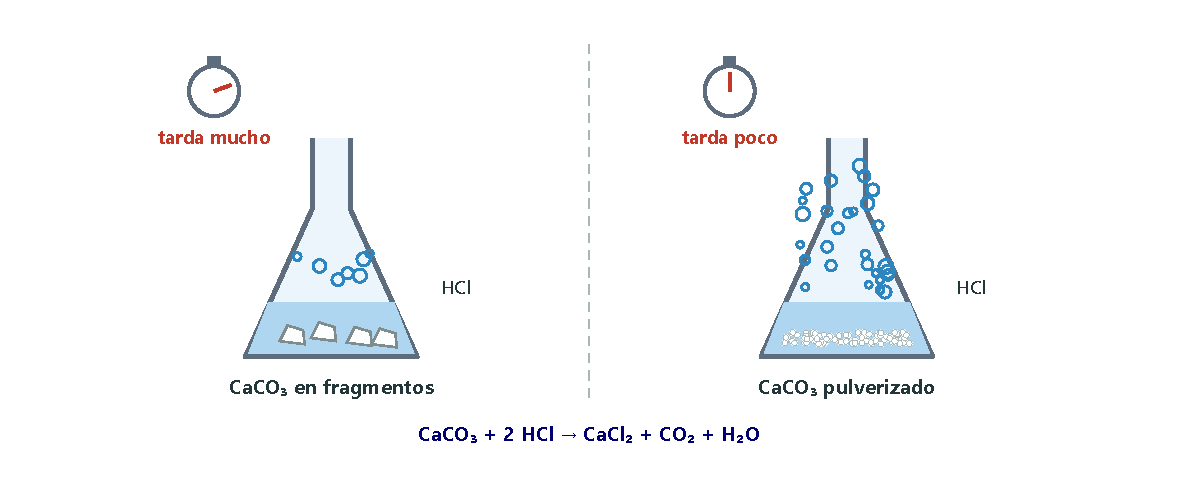
\includegraphics[width=0.8\textwidth]{images/UD1/practica_superficie}
    \caption{Reacción del carbonato de calcio en fragmentos y pulverizado con ácido clorhídrico.}
    \label{fig:practica_superficie}
\end{figure}

\noindent\begin{minipage}[t]{0.5\textwidth}
    \textbf{Objetivos}
    \begin{itemize}
        \item Comprobar una hipótesis mediante la experimentación.
        \item Medir masas, volúmenes y tiempos.
        \item Trabajar con seguridad en el laboratorio.
    \end{itemize}
\end{minipage}\hfill
\begin{minipage}[t]{0.46\textwidth}
    \textbf{Material}
    \begin{itemize}
        \item Balanza, probeta, dos Erlenmeyer y dos vidrios de reloj.
        \item Carbonato de calcio y ácido clorhídrico diluido.
        \item Un cronómetro.
    \end{itemize}
\end{minipage}

\medskip

\textbf{Procedimiento}
\begin{enumerate}[label=\numberballgreen]
    \item Pesa dos muestras iguales de carbonato de calcio: una en fragmentos y otra pulverizada.
    \item Pon el carbonato en fragmentos en un Erlenmeyer, añade un volumen medido de ácido clorhídrico y pon en marcha el cronómetro. Detenlo cuando desaparezca todo el sólido.
    \item Repite la experiencia con el carbonato pulverizado, la misma cantidad de ácido y el mismo cronómetro.
\end{enumerate}

\begin{exercise}
    Responde a estas preguntas sobre la práctica:
    \begin{enumerate}[label=\alph*)]
        \item ¿Cuál es la variable independiente? ¿Y la dependiente? ¿Qué variables deben estar controladas?
        \item ¿Por qué es importante usar el mismo cronómetro y la misma cantidad de ácido?
        \item Un grupo obtiene \qty{185}{\s} con los fragmentos y \qty{40}{\s} con el polvo. ¿Se confirma la hipótesis? ¿Cuántas veces más rápida ha sido la reacción con el polvo?
    \end{enumerate}
    \begin{solu}
        a) Independiente: el \textcolor{red}{grado de división} del sólido (superficie de contacto). Dependiente: el \textcolor{red}{tiempo} que tarda en desaparecer. Controladas: la \textcolor{red}{masa} de carbonato, el \textcolor{red}{volumen y la concentración} del ácido, la temperatura\ldots
        b) Para que solo cambie la variable que estudiamos y las medidas sean \textcolor{red}{comparables}.
        c) \textcolor{red}{Sí}: con el polvo la reacción termina antes. Es \(\dfrac{185}{40} = \textcolor{red}{\num{4.6}}\) veces más rápida.
    \end{solu}
\end{exercise}

%========================================================================================
\section{Unidad 2. Propiedades de los elementos}
%========================================================================================
% (sacado del final de UD_2_el_atomo_tp.tex)

Vamos a comprobar experimentalmente algunas propiedades que distinguen a los metales de los no metales, usando tres metales (cobre, aluminio y zinc) y un no metal (carbono en forma de grafito, la mina de un lápiz).

\begin{multicols}{2}
    \textbf{Objetivos}
    \begin{itemize}
        \item Manejar materiales e instrumentos del laboratorio de Química.
        \item Respetar las normas de seguridad.
        \item Comprobar la conductividad, la solubilidad en agua y la reacción con ácido clorhídrico de varios elementos.
    \end{itemize}
    \columnbreak
    \textbf{Material}
    \begin{itemize}
        \item Cobre, aluminio, zinc y grafito.
        \item Un circuito sencillo (pila, cables y bombilla o LED).
        \item Ácido clorhídrico diluido (\ch{HCl}), agua.
        \item Vaso de precipitados y tubos de ensayo.
    \end{itemize}
\end{multicols}

\textbf{Procedimiento}
\begin{enumerate}[label=\numberballgreen]
    \item Observa el aspecto de cada elemento (¿tiene brillo metálico?).
    \item Echa un poco de cada uno en un tubo de ensayo con agua y comprueba si se disuelve.
    \item Pon un trozo de zinc en un tubo con unos mililitros de ácido clorhídrico y observa si hay reacción (burbujas). Repite con los demás elementos. \textbf{Usa gafas y guantes.}
    \item Intercala cada elemento en el circuito y comprueba si la bombilla se enciende.
\end{enumerate}

\begin{exercise}
    Recoge tus resultados en una tabla con las columnas: elemento, aspecto, densidad, solubilidad en agua, reacción con \ch{HCl} y conductividad eléctrica (busca las densidades en Internet). ¿Conduce el grafito la corriente? ¿Es eso habitual en los no metales? ¿Qué gas se desprende cuando el ácido reacciona con el zinc y el aluminio? ¿Cómo medirías la densidad de cada elemento en el laboratorio?
    \begin{solu}
        \begin{center}
            % --- tabla antigua ---
            % \begin{tblr}{colspec={lccccc}, hlines, vlines, row{1}={font=\bfseries}}
                % Elemento & Aspecto & Densidad (\unit{\gram\per\cubic\centi\metre}) & Solubilidad & Con \ch{HCl} & Conduce \\
                % Aluminio & metálico & \num{2.70} & insoluble & desprende \ch{H2} & sí \\
                % Grafito & no metálico & \num{2.26} & insoluble & no reacciona & sí \\
                % Zinc & metálico & \num{7.14} & insoluble & desprende \ch{H2} & sí \\
                % Cobre & metálico & \num{8.96} & insoluble & no reacciona & sí \\
            % \end{tblr}
            % --- tabla nueva ---
            \begin{tabular}{@{}lccccc@{}}
                \toprule
                \textbf{Elemento} & \textbf{Aspecto} & \textbf{Densidad (\unit{\gram\per\cubic\centi\metre})} & \textbf{Solubilidad} & \textbf{Con \ch{HCl}} & \textbf{Conduce} \\
                \midrule
                Aluminio & metálico & \num{2.70} & insoluble & desprende \ch{H2} & sí \\[3pt]
                Grafito & no metálico & \num{2.26} & insoluble & no reacciona & sí \\[3pt]
                Zinc & metálico & \num{7.14} & insoluble & desprende \ch{H2} & sí \\[3pt]
                Cobre & metálico & \num{8.96} & insoluble & no reacciona & sí \\
                \bottomrule
            \end{tabular}
        \end{center}
        El grafito conduce la corriente, pero es una excepción: los no metales, en general, no conducen. El gas desprendido es \textcolor{red}{hidrógeno}, \ch{H2}. La densidad se calcula midiendo la masa con una balanza y el volumen por desplazamiento de agua en una probeta: \(d = m/V\).
    \end{solu}
\end{exercise}

%========================================================================================
\section{Unidad 3. Propiedades de las sustancias y enlace químico}
%========================================================================================
% (sacado del final de UD3_enlace_quimico.tex)

Vamos a estudiar algunas propiedades del sulfato de cobre(II), \ch{CuSO4}, el cloruro de potasio, \ch{KCl}, y el dióxido de silicio, \ch{SiO2} (arena fina), en estado sólido y en disolución. A partir de los resultados deduciremos qué tipo de enlace tiene cada sustancia.

\begin{multicols}{2}
    \textbf{Objetivos}
    \begin{itemize}
        \item Manejar materiales e instrumentos del laboratorio de Química.
        \item Respetar las normas de seguridad.
        \item Valorar la importancia del trabajo experimental sistemático.
        \item Comprobar la dureza, la solubilidad y la conductividad eléctrica de varias sustancias.
    \end{itemize}
    \columnbreak
    \textbf{Material}
    \begin{itemize}
        \item \ch{CuSO4}, \ch{KCl} y \ch{SiO2}; un clavo.
        \item Agua destilada, tetracloruro de carbono (\ch{CCl4}), seis tubos de ensayo y una gradilla.
        \item Pila de \qty{9}{\volt} o \qty{12}{\volt}, cables con pinzas de cocodrilo, bombilla o LED, dos electrodos, cápsula de porcelana y vaso de precipitados.
    \end{itemize}
\end{multicols}

\textbf{Procedimiento}
\begin{enumerate}[label=\numberballgreen]
    \item \textbf{Dureza.} Intenta rayar cada sustancia con la punta de un clavo y anota lo que observas.
    \item \textbf{Solubilidad en agua} (disolvente polar). Pon un poco de cada sustancia en un tubo de ensayo, añade agua destilada hasta la mitad y agita. Anota cuáles se disuelven.
    \item \textbf{Solubilidad en tetracloruro de carbono} (disolvente apolar). Repite el paso anterior con \ch{CCl4} (hasta un tercio del tubo). \textbf{Hazlo en la vitrina de gases, con gafas y guantes.}
    \item \textbf{Conductividad del sólido.} Coloca cada sólido en la cápsula de porcelana, introduce los electrodos y comprueba si se enciende la bombilla.
    \item \textbf{Conductividad de la disolución.} Repite la prueba con las disoluciones acuosas de las sustancias que se hayan disuelto.
\end{enumerate}

\begin{exercise}
    Recoge tus resultados en una tabla con las columnas: dureza, solubilidad en agua, solubilidad en \ch{CCl4}, conductividad en estado sólido y conductividad en disolución acuosa, para el \ch{CuSO4}, el \ch{KCl} y el \ch{SiO2}.
    \begin{solu}
        Respuesta según los resultados del laboratorio. Lo esperable es:
        \begin{center}
            % --- tabla antigua ---
            % \begin{tblr}{colspec={lccccc}, hlines, vlines, row{1}={font=\bfseries}}
                % & Dureza & Agua & \ch{CCl4} & Sólido & Disolución \\
                % \ch{CuSO4} & duro, frágil & soluble & insoluble & no conduce & conduce \\
                % \ch{KCl} & duro, frágil & soluble & insoluble & no conduce & conduce \\
                % \ch{SiO2} & muy duro & insoluble & insoluble & no conduce & --- \\
            % \end{tblr}
            % --- tabla nueva ---
            \begin{tabular}{@{}lccccc@{}}
                \toprule
                 & \textbf{Dureza} & \textbf{Agua} & \textbf{\ch{CCl4}} & \textbf{Sólido} & \textbf{Disolución} \\
                \midrule
                \ch{CuSO4} & duro, frágil & soluble & insoluble & no conduce & conduce \\[3pt]
                \ch{KCl} & duro, frágil & soluble & insoluble & no conduce & conduce \\[3pt]
                \ch{SiO2} & muy duro & insoluble & insoluble & no conduce & --- \\
                \bottomrule
            \end{tabular}
        \end{center}
    \end{solu}
\end{exercise}

\begin{exercise}
    A partir de tus resultados, ¿qué tipo de enlace tiene cada sustancia? ¿Qué propiedades físicas y químicas presentan?
    \begin{solu}
        \textcolor{red}{\ch{CuSO4}: iónico} (entre el catión \ch{Cu^{2+}} y el anión \ch{SO4^{2-}}). Es soluble en agua y no conduce en estado sólido, pero sí disuelto.
        \textcolor{red}{\ch{KCl}: iónico} (entre \ch{K+} y \ch{Cl-}). Mismo comportamiento: soluble en agua y conductor solo en disolución.
        \textcolor{red}{\ch{SiO2}: covalente reticular}. Es muy duro, insoluble en agua y en \ch{CCl4} y no conduce la corriente.
    \end{solu}
\end{exercise}

%========================================================================================
\section[Unidad 4. Carbono en un compuesto]{Unidad 4. Investigación de la existencia de carbono en un compuesto}
%========================================================================================
% (sacado del final de UD4_organica.tex)

Vamos a comprobar si una sustancia contiene carbono. Al calentarla con óxido de cobre(II), el carbono se oxida a dióxido de carbono, \ch{CO2}. Si este gas se hace burbujear en una disolución de hidróxido de calcio (agua de cal), se forma carbonato de calcio, \ch{CaCO3}, un sólido blanco insoluble en agua (es el componente principal de la roca caliza):
\[ \ch{Ca(OH)2 (aq) + CO2 (g) -> CaCO3 (s) + H2O (l)} \]

\begin{figure}[H]
    \centering
    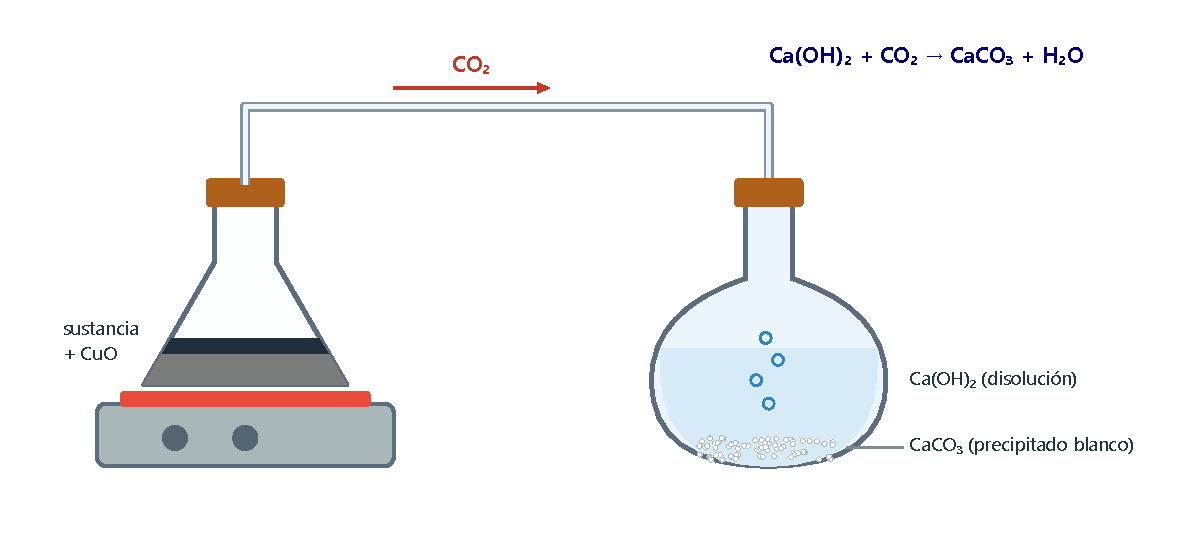
\includegraphics[width=0.9\textwidth]{images/UD4/practica_carbono}
    \caption{Montaje para detectar el carbono de un compuesto.}
    \label{fig:practica_carbono}
\end{figure}

\noindent\begin{minipage}[t]{0.48\textwidth}
    \textbf{Objetivos}
    \begin{itemize}
        \item Detectar la presencia de carbono en un compuesto.
        \item Trabajar con materiales e instrumentos del laboratorio.
        \item Respetar las normas de seguridad al manejar sustancias peligrosas.
    \end{itemize}
\end{minipage}\hfill
\begin{minipage}[t]{0.48\textwidth}
    \textbf{Material}
    \begin{itemize}
        \item Un matraz Erlenmeyer y un matraz aforado, con tapones horadados.
        \item Una placa calefactora y un tubo de vidrio en doble L.
        \item Hidróxido de calcio y óxido de cobre(II).
        \item Una sustancia con carbono (azúcar, almidón\ldots).
    \end{itemize}
\end{minipage}

\medskip

\textbf{Procedimiento}
\begin{enumerate}[label=\numberballgreen]
    \item Pon en el Erlenmeyer una mezcla de la sustancia con aproximadamente el triple de óxido de cobre(II) en polvo, previamente calcinado, y cubre la mezcla con más óxido de cobre.
    \item Cierra el Erlenmeyer con el tapón y el tubo de desprendimiento en doble L.
    \item Introduce el otro extremo del tubo en una disolución de hidróxido de calcio contenida en el matraz aforado, cerrado con el otro tapón (figura~\ref{fig:practica_carbono}).
    \item Calienta la mezcla para que los gases que se desprenden burbujeen en la disolución.
\end{enumerate}

\begin{exercise}
    Responde a estas preguntas sobre la práctica:
    \begin{enumerate}[label=\alph*)]
        \item Describe lo que sucede en el matraz aforado. ¿Qué significa?
        \item ¿Qué confirma que la sustancia de partida contiene carbono?
        \item ¿De dónde procede el \ch{CO2}? ¿Qué le ocurre al \ch{CaCO3}?
        \item ¿Qué sucedería si soplaras a través de un tubo sumergido en la disolución de hidróxido de calcio? ¿Por qué?
    \end{enumerate}
    \begin{solu}
        a) Se desprenden burbujas de un gas y la disolución \textcolor{red}{se enturbia}: se ha formado un sólido blanco. Significa que se ha desprendido \ch{CO2}.
        b) La formación del \textcolor{red}{precipitado blanco de carbonato de calcio}.
        c) El \ch{CO2} procede de la reacción del \textcolor{red}{carbono de la sustancia con el óxido de cobre(II)}, que aporta el oxígeno. El \ch{CaCO3} es insoluble y \textcolor{red}{precipita}.
        d) También se \textcolor{red}{enturbiaría}, porque el aire que expulsamos contiene \ch{CO2}, procedente de la oxidación de los compuestos del carbono de los alimentos en las células.
    \end{solu}
\end{exercise}

%========================================================================================
\section{Unidad 5. Separación de una mezcla de alcohol y agua}
%========================================================================================
% (sacado del final de UD5_Sistema_materiales.tex)

El alcohol (etanol) y el agua tienen temperaturas de ebullición distintas, así que podemos separarlos por \textbf{destilación} (figura~\ref{fig:separacion_disoluciones}).

\begin{multicols}{2}
    \textbf{Objetivos}
    \begin{itemize}
        \item Manejar materiales e instrumentos del laboratorio.
        \item Respetar las normas de seguridad.
        \item Valorar el trabajo experimental sistemático.
        \item Separar los componentes de una disolución de alcohol y agua.
    \end{itemize}
    \columnbreak
    \textbf{Material}
    \begin{itemize}
        \item Matraz de destilación (o matraz con cabeza de destilación) y termómetro.
        \item Placa calefactora, cristalizador (baño María), dos soportes con pinzas.
        \item Refrigerante con gomas de entrada y salida de agua.
        \item Erlenmeyer, probeta de \qty{100}{\mL}, alcohol y agua.
    \end{itemize}
\end{multicols}

\textbf{Procedimiento}
\begin{enumerate}[label=\numberballgreen]
    \item Prepara una disolución de alcohol en agua al \qty{90}{\percent} en volumen.
    \item Monta el aparato de destilación y pon la disolución en el matraz.
    \item Conecta la goma de entrada de agua a la parte baja del refrigerante y lleva la de salida al fregadero.
    \item Calienta el matraz con la placa calefactora o al baño María. \textbf{El alcohol es inflamable: nunca uses una llama.}
    \item Anota la temperatura cuando el alcohol empiece a destilar: verás que se mantiene constante.
    \item Deja de calentar cuando la temperatura empiece a subir de nuevo.
\end{enumerate}

\begin{exercise}
    Responde a estas preguntas sobre la práctica:
    \begin{enumerate}[label=\alph*)]
        \item ¿Para qué sirve el refrigerante?
        \item ¿Por qué el agua entra por la parte baja del refrigerante y sale por la alta, y no al revés?
        \item ¿Para qué sirve el termómetro? ¿Qué temperatura marca cuando el alcohol empieza a destilar?
        \item ¿Durante cuánto tiempo se mantiene constante la temperatura? ¿Qué ocurre cuando empieza a subir?
        \item ¿Qué se recoge en el Erlenmeyer y qué queda en el matraz de destilación?
    \end{enumerate}
    \begin{solu}
        a) Para \textcolor{red}{enfriar el vapor} que sale del matraz y condensarlo, de modo que se pueda recoger como líquido.
        b) Así el agua fría recorre el refrigerante en sentido contrario al vapor, el tubo se llena bien de agua y el vapor se encuentra con agua cada vez más fría a medida que avanza.
        c) Para controlar la temperatura del vapor y saber qué sustancia destila. Unos \textcolor{red}{\qty{78}{\celsius}}, la temperatura de ebullición del etanol.
        d) Mientras queda alcohol por evaporar, porque la energía se emplea en el cambio de estado. Cuando sube, \textcolor{red}{ya se ha separado todo el alcohol} y se está calentando el agua.
        e) En el Erlenmeyer, el \textcolor{red}{alcohol}; en el matraz, el \textcolor{red}{agua}.
    \end{solu}
\end{exercise}

%========================================================================================
\section{Unidad 6. Estudio de una reacción de neutralización}
%========================================================================================
% (sacado del final de UD6_reacciones_quimicas.tex)

Vamos a usar una reacción de neutralización para averiguar la concentración de una disolución de \ch{HCl} (una \textbf{valoración}) y aprenderemos a usar un pH-metro. Es un instrumento delicado: el electrodo no debe chocar con el vaso ni con el agitador, hay que lavarlo con agua destilada después de cada medida y guardarlo sumergido en agua destilada.

\begin{multicols}{2}
    \textbf{Objetivos}
    \begin{itemize}
        \item Trabajar con sustancias e instrumentos del laboratorio de Química.
        \item Respetar las normas de seguridad con sustancias peligrosas e instrumentos delicados.
        \item Determinar la concentración de una disolución de \ch{HCl}.
    \end{itemize}
    \columnbreak
    \textbf{Material}
    \begin{itemize}
        \item Disolución de \ch{NaOH} \num{0.1} M y disolución de \ch{HCl} de concentración desconocida.
        \item Bureta, pipeta, matraz Erlenmeyer, agitador magnético, soporte con pinza.
        \item Fenolftaleína y pH-metro.
    \end{itemize}
\end{multicols}

\textbf{Procedimiento}
\begin{enumerate}[label=\numberballgreen]
    \item Sujeta la bureta al soporte y llénala con la disolución de \ch{NaOH} \num{0.1} M, enrasando el menisco en una división.
    \item Con la pipeta, pon un volumen conocido de \ch{HCl} en el Erlenmeyer y mide su pH.
    \item Añade unas gotas de fenolftaleína y coloca el Erlenmeyer sobre el agitador, debajo de la bureta.
    \item Deja caer gota a gota la disolución de \ch{NaOH} mientras se agita, hasta que el indicador cambie de color (el cambio es muy rápido). Anota el volumen gastado.
    \item Mide de nuevo el pH con el pH-metro.
\end{enumerate}

\begin{figure}[H]
    \centering
    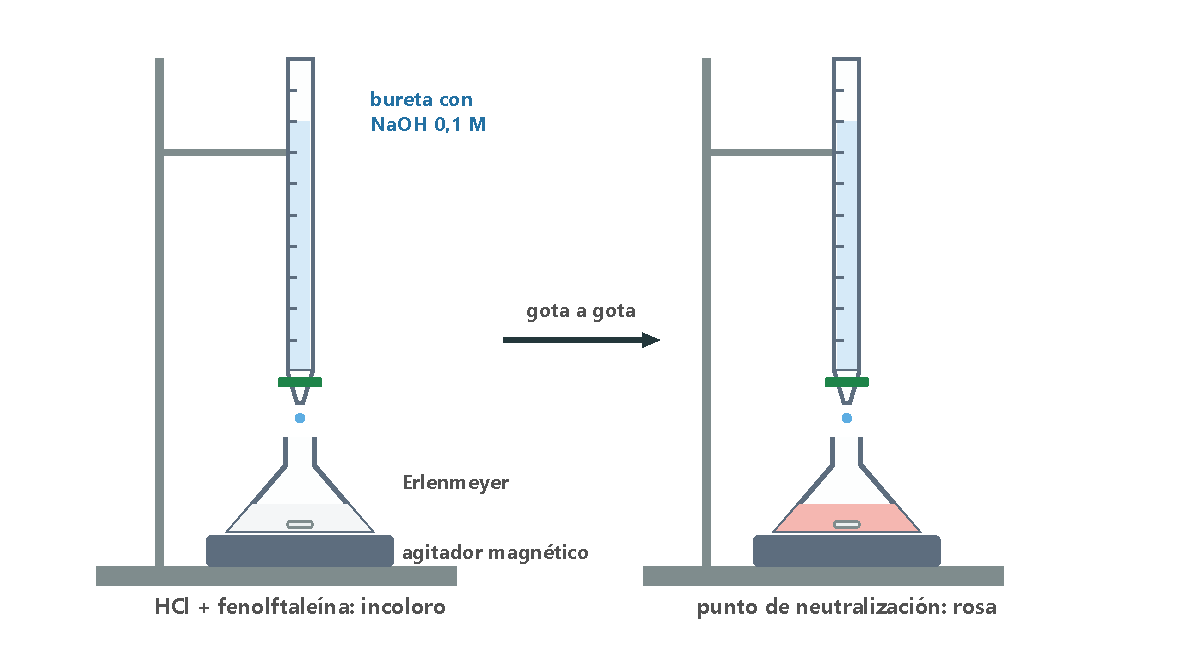
\includegraphics[width=0.75\textwidth]{images/UD6/valoracion}
    \caption{Valoración de un ácido con una base.}
    \label{fig:valoracion}
\end{figure}

\begin{exercise}
    Responde a estas preguntas sobre la práctica:
    \begin{enumerate}[label=\alph*)]
        \item ¿De qué color está la fenolftaleína en la disolución de \ch{HCl}? ¿Y después de la neutralización?
        \item Escribe la ecuación de la reacción.
        \item ¿Para qué sirve el agitador magnético?
        \item ¿Por qué hay que lavar el electrodo del pH-metro y guardarlo en agua destilada?
        \item Si se gastan \qty{20}{\mL} de \ch{NaOH} \num{0.1} M para neutralizar \qty{25}{\mL} de \ch{HCl}, ¿cuál es la concentración del ácido? (En el punto de neutralización, moles de \ch{NaOH} = moles de \ch{HCl}.)
    \end{enumerate}
    \begin{solu}
        a) \textcolor{red}{Incolora} en el ácido; \textcolor{red}{rosa} cuando se ha neutralizado (en cuanto hay un ligero exceso de base).
        b) \ch{HCl (aq) + NaOH (aq) -> NaCl (aq) + H2O (l)}.
        c) Para \textcolor{red}{mezclar} bien la disolución y que la base reaccione en cuanto cae.
        d) Para \textcolor{red}{no cometer errores} de medida (que no queden restos de otra disolución) y para que el electrodo no se seque y se estropee.
        e) \(n(\ch{NaOH}) = \num{0.1} \cdot \num{0.020} = \qty{0.002}{\mol} = n(\ch{HCl})\); \(M(\ch{HCl}) = \frac{\num{0.002}}{\num{0.025}} = \textcolor{red}{\qty{0.08}{\mol\per\L}}\).
    \end{solu}
\end{exercise}

%========================================================================================
\section{Unidad 7. La experiencia de Galileo}
%========================================================================================
% (sacado del final de UD7_movimientos_rectilineos.tex)

En un MRUA que parte del reposo, el espacio recorrido es proporcional al cuadrado del tiempo: \(s = \frac{1}{2}\, a\, t^2\). Galileo lo comprobó dejando rodar una bola por un carril inclinado y midiendo el tiempo con un \emph{reloj de agua}: el volumen de agua que caía de un depósito mientras la bola recorría el carril. Vamos a repetir su experiencia.

\begin{figure}[H]
    \centering
    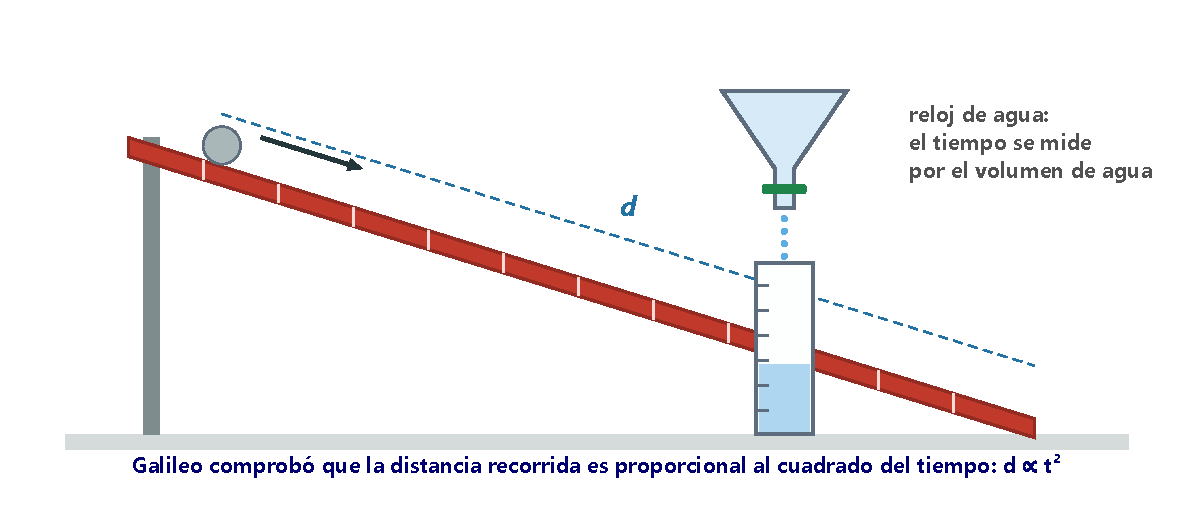
\includegraphics[width=0.75\textwidth]{images/UD7/plano_galileo}
    \caption{Montaje para repetir la experiencia de Galileo.}
    \label{fig:plano_galileo}
\end{figure}

\begin{multicols}{2}
    \textbf{Objetivos}
    \begin{itemize}
        \item Trabajar con materiales del laboratorio de Física y Química.
        \item Respetar las normas de seguridad.
        \item Valorar el trabajo experimental sistemático.
        \item Comprobar la relación entre espacio y tiempo en un MRUA.
    \end{itemize}
    \columnbreak
    \textbf{Material}
    \begin{itemize}
        \item Un carril acanalado de al menos \qty{1}{\m}.
        \item Un embudo con llave y soporte, y una probeta graduada (o un cronómetro).
        \item Una bolita metálica y una cinta métrica.
    \end{itemize}
\end{multicols}

\textbf{Procedimiento}
\begin{enumerate}[label=\numberballgreen]
    \item Fija el carril con una inclinación pequeña y marca la distancia \(d\) entre la bolita y el final del carril.
    \item Llena el embudo de agua y colócalo sobre la probeta.
    \item Suelta la bolita a la vez que abres la llave, y ciérrala cuando la bolita llegue al final. El tiempo se mide en mL de agua (o con el cronómetro).
    \item Repite la experiencia para cuatro distancias distintas (y varias veces cada una).
\end{enumerate}

\begin{exercise}
    Anota tus resultados en una tabla con las columnas \(d\) (m), \(t\) y \(t^2\), compáralos con los del resto de la clase y represéntalos en dos gráficas: \(d\) frente a \(t\) y \(d\) frente a \(t^2\).
    \begin{enumerate}[label=\alph*)]
        \item ¿Qué forma tiene la gráfica \(d\)-\(t\)? ¿Por qué?
        \item ¿Qué relación encuentras entre \(d\) y \(t^2\)?
    \end{enumerate}
    \begin{solu}
        Respuesta según los datos del laboratorio. a) La gráfica \(d\)-\(t\) es una \textcolor{red}{parábola} (curva), porque en un MRUA el espacio no es proporcional al tiempo. b) La gráfica \(d\)-\(t^2\) es una \textcolor{red}{recta que pasa por el origen}: \(d\) es \textcolor{red}{directamente proporcional a \(t^2\)}, y la pendiente vale \(\frac{a}{2}\).
    \end{solu}
\end{exercise}

%========================================================================================
\section{Unidad 8. Factores que afectan a la fuerza de rozamiento}
%========================================================================================
% (sacado del final de UD8_fuerzas.tex)

Vamos a hacer unos experimentos sencillos para averiguar de qué depende la fuerza de rozamiento entre dos cuerpos, con el montaje de la figura~\ref{fig:rozamiento_montaje}.

\begin{multicols}{2}
    \textbf{Objetivos}
    \begin{itemize}
        \item Trabajar con materiales e instrumentos del laboratorio de Física.
        \item Respetar las normas de seguridad.
        \item Valorar el trabajo experimental sistemático.
        \item Comprobar algunos factores de los que depende la fuerza de rozamiento.
    \end{itemize}
    \columnbreak
    \textbf{Material}
    \begin{itemize}
        \item Un sistema de polea y portapesas.
        \item Un bloque de madera de masa conocida y otro de plástico de la misma masa.
        \item Varias pesas de \qty{0.1}{\kg} a \qty{0.5}{\kg}.
        \item Un dinamómetro (puede sustituir al portapesas).
    \end{itemize}
\end{multicols}

\textbf{Procedimiento}
\begin{enumerate}[label=\numberballgreen]
    \item Monta el sistema y añade poco a poco pesas al portapesas (o tira con el dinamómetro) hasta que el bloque de madera empiece a deslizar. Anota el peso del portapesas.
    \item Coloca una pesa de \qty{0.1}{\kg} sobre el bloque y repite la medida. Repítelo con dos y con tres pesas.
    \item Apoya el bloque sobre otra de sus caras (de distinta área) y repite la medida.
    \item Repite el paso 1 con el bloque de plástico.
\end{enumerate}

\begin{exercise}
    Responde a estas preguntas sobre la práctica:
    \begin{enumerate}[label=\alph*)]
        \item ¿Cómo mides la fuerza de rozamiento entre el bloque y la mesa?
        \item Anota en una tabla el peso del bloque (con 0, 1, 2 y 3 pesas) y la fuerza de rozamiento. ¿Qué relación encuentras?
        \item ¿Cambia la fuerza de rozamiento al apoyar el bloque sobre otra cara?
        \item ¿Cómo influye la naturaleza de las superficies (madera o plástico)?
    \end{enumerate}
    \begin{solu}
        Respuesta según los datos del laboratorio. Lo esperable es:
        a) Cuando el bloque empieza a moverse, la fuerza aplicada \textcolor{red}{iguala} a la de rozamiento: esta es el peso del portapesas (o lo que marca el dinamómetro).
        b) La fuerza de rozamiento es \textcolor{red}{proporcional al peso} del bloque (a la normal): al duplicar el peso, se duplica. El cociente \(F_\text{roz}/N\) es el coeficiente de rozamiento.
        c) \textcolor{red}{No}: no depende del área de contacto.
        d) Con superficies distintas el rozamiento es \textcolor{red}{distinto}: depende de la naturaleza de las superficies (normalmente el plástico liso roza menos que la madera).
    \end{solu}
\end{exercise}

%========================================================================================
\section[Unidad 9. La gravedad con un péndulo]{Unidad 9. Cálculo de la gravedad con un péndulo simple}
%========================================================================================
% (sacado del final de UD9_movimiento_circular.tex)

Un \textbf{péndulo simple} es una bolita pesada colgada de un hilo que puede oscilar libremente alrededor de su posición de equilibrio. Si las oscilaciones son pequeñas, el tiempo que tarda en ir y volver (su período) solo depende de la longitud del hilo, \(L\), y de la gravedad, \(g\):
\[ T = 2\pi \sqrt{\frac{L}{g}} \qquad\Rightarrow\qquad g = \frac{4\pi^2 \cdot L}{T^2} \]
Midiendo \(L\) y \(T\) podemos calcular \(g\) en el laboratorio.

\begin{figure}[H]
    \centering
    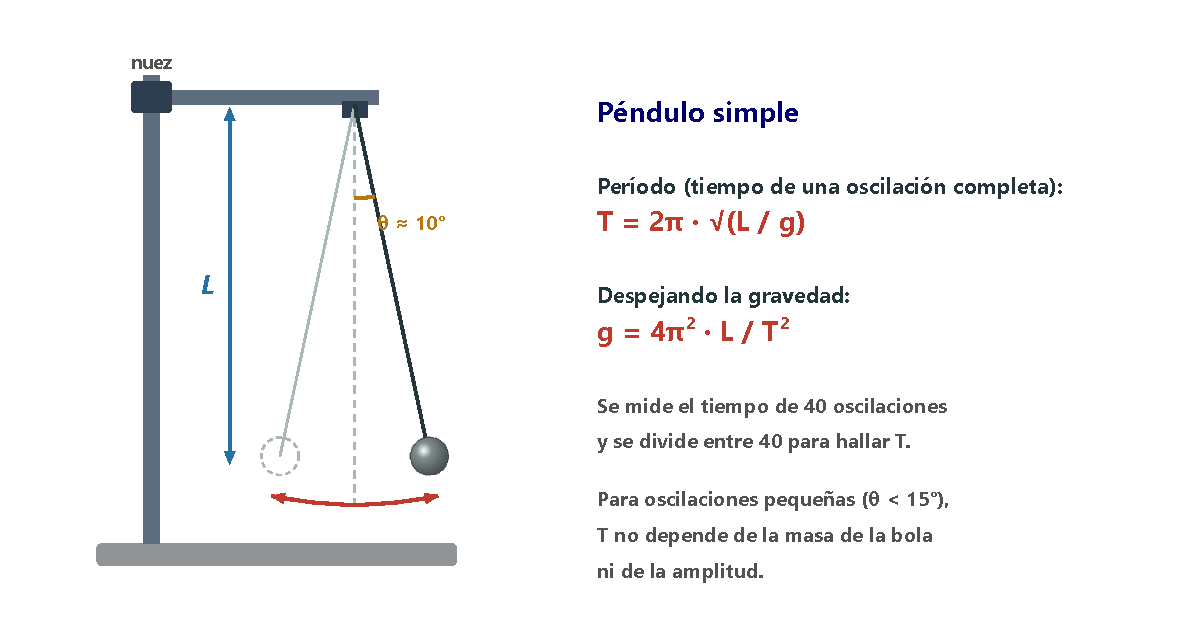
\includegraphics[width=0.8\textwidth]{images/UD9/pendulo}
    \caption{Montaje del péndulo simple.}
    \label{fig:pendulo}
\end{figure}

\noindent\begin{minipage}{\textwidth}
\begin{multicols}{2}
    \textbf{Objetivos}
    \begin{itemize}
        \item Trabajar con materiales e instrumentos del laboratorio de Física.
        \item Valorar el trabajo experimental sistemático.
        \item Medir longitudes y tiempos con los instrumentos adecuados.
        \item Calcular la aceleración de la gravedad a partir de medidas indirectas.
    \end{itemize}
    \columnbreak
    \textbf{Material}
    \begin{itemize}
        \item Un soporte con una pinza metálica y una nuez.
        \item Un hilo de longitud \(L\) (por ejemplo, \qty{1}{\m}) y una cinta métrica.
        \item Una bolita pesada (mejor metálica) con enganche.
        \item Un cronómetro y un transportador de ángulos.
    \end{itemize}
\end{multicols}
\end{minipage}

\textbf{Procedimiento}
\begin{enumerate}[label=\numberballgreen]
    \item Monta el péndulo como en la figura~\ref{fig:pendulo}. Mide la longitud \(L\) desde el punto de suspensión hasta el centro de la bolita.
    \item Separa la bolita unos \ang{10} de la posición de equilibrio y suéltala sin empujarla. Las oscilaciones no deben ser muy abiertas.
    \item Cronometra el tiempo de 40 oscilaciones completas y divídelo entre 40 para obtener el período. Repite la medida al menos cinco veces.
\end{enumerate}

\begin{exercise}
    Responde a estas preguntas sobre la práctica:
    \begin{enumerate}[label=\alph*)]
        \item Anota en una tabla, para cada medida, el tiempo de 40 oscilaciones, el período y el valor de \(g\). ¿Por qué medimos 40 oscilaciones en lugar de una sola?
        \item Calcula la media de los valores de \(g\) y compárala con \qty{9.8}{\m\per\square\s}.
        \item ¿En qué pasos del experimento se cometen más errores de medida?
        \item Con un hilo de \qty{1.00}{\m}, un grupo mide \qty{80.4}{\s} para 40 oscilaciones. ¿Qué valor de \(g\) obtiene?
    \end{enumerate}
    \begin{solu}
        a) Respuesta según los datos. Medir 40 oscilaciones es \textcolor{red}{más fácil y más preciso}: el error al poner en marcha y parar el cronómetro (unas décimas de segundo) se reparte entre las 40 oscilaciones.
        b) Respuesta libre; el resultado suele estar cerca de \qty{9.8}{\m\per\square\s}, aunque los errores de medida pueden ser importantes.
        c) Al \textcolor{red}{medir la longitud del hilo} (hay que llegar hasta el centro de la bola) y al \textcolor{red}{medir el tiempo} (tiempo de reacción).
        d) \(T = \dfrac{\num{80.4}}{40} = \qty{2.01}{\s}\); \(g = \dfrac{4\pi^2 \cdot \num{1.00}}{\num{2.01}^2} = \textcolor{red}{\qty{9.77}{\m\per\square\s}}\).
    \end{solu}
\end{exercise}

%========================================================================================
\section[Unidad 10. Principio de Arquímedes]{Unidad 10. Comprobación del principio de Arquímedes}
%========================================================================================
% (sacado del final de UD10_fluidos.tex)

Vamos a comprobar que un cuerpo sumergido en agua recibe un empuje igual al peso del agua que desaloja:
\[ \text{Empuje} = \text{peso en el aire} - \text{peso en el agua} = \text{peso del agua desalojada} \]


\noindent\begin{minipage}[t]{0.53\textwidth}
    \textbf{Objetivos}
    \begin{itemize}
        \item Trabajar con materiales e instrumentos del laboratorio de Física.
        \item Valorar el trabajo experimental sistemático, evitando errores de paralaje.
        \item Comprobar la relación entre el empuje, el peso en el aire y el peso en el agua de un cuerpo.
        \item Calcular la densidad de un cuerpo.
    \end{itemize}
\end{minipage}\hfill
\begin{minipage}[t]{0.43\textwidth}
    \textbf{Material}
    \begin{itemize}
        \item Un soporte con una pinza metálica y una nuez.
        \item Un dinamómetro y una probeta graduada.
        \item Una esfera de metal con enganche e hilo.
        \item Agua.
    \end{itemize}
\end{minipage}

\medskip

\textbf{Procedimiento} (el montaje es como el de la figura~\ref{fig:empuje})
\begin{enumerate}[label=\numberballgreen]
    \item Cuelga la esfera del dinamómetro y anota su peso en el aire.
    \item Echa agua en la probeta, hasta la mitad aproximadamente, y mide su volumen con cuidado: mira la escala con los ojos a la altura de la superficie del agua para no cometer \textbf{error de paralaje}.
    \item Sumerge la esfera, colgada del dinamómetro, en el agua de la probeta, de modo que quede totalmente cubierta pero sin tocar el fondo. Anota su peso y el nuevo nivel del agua.
    \item Repite el procedimiento tres veces y anota los resultados en una tabla como esta:
\end{enumerate}

\begin{center}
    % --- tabla antigua ---
    % \begin{tblr}{width=\linewidth, colspec={Q[c,m] X[c,m] X[c,m] X[c,m] X[c,m] X[c,m]}, hlines, vlines, row{1}={bg=ocre!85, fg=white, font=\bfseries\small}, cells={font=\small}}
        % Exp. & Peso en el aire (N) & Peso en el agua (N) & Empuje (N) & Volumen inicial (\unit{\cubic\cm}) & Volumen final (\unit{\cubic\cm}) \\
        % 1 & \ldots & \ldots & \ldots & \ldots & \ldots \\
        % 2 & \ldots & \ldots & \ldots & \ldots & \ldots \\
        % 3 & \ldots & \ldots & \ldots & \ldots & \ldots \\
    % \end{tblr}
    % --- tabla nueva ---
    {\small
    \begin{tabular}{@{}c c c c C{0.15\linewidth} C{0.15\linewidth}@{}}
        \toprule
        \textbf{Exp.} & \textbf{Peso en el aire (N)} & \textbf{Peso en el agua (N)} & \textbf{Empuje (N)} & \textbf{Volumen inicial (\unit{\cubic\cm})} & \textbf{Volumen final (\unit{\cubic\cm})} \\
        \midrule
        1 & \ldots & \ldots & \ldots & \ldots & \ldots \\[3pt]
        2 & \ldots & \ldots & \ldots & \ldots & \ldots \\[3pt]
        3 & \ldots & \ldots & \ldots & \ldots & \ldots \\
        \bottomrule
    \end{tabular}
    }
\end{center}

\begin{exercise}
    Responde a estas preguntas sobre la práctica:
    \begin{enumerate}[label=\alph*)]
        \item ¿Cuándo pesa más la esfera, antes o después de sumergirla? Calcula el empuje con los valores medios.
        \item Calcula el volumen de agua desalojada (aumento de volumen en la probeta). ¿Qué relación tiene con el volumen de la esfera?
        \item Calcula el peso del agua desalojada y compáralo con el empuje.
        \item Calcula la densidad de la esfera.
        \item ¿Qué empuje recibiría la esfera en alcohol (\qty{790}{\kg\per\cubic\m})?
        \item Un grupo obtiene estos valores medios: peso en el aire, \qty{2.40}{\newton}; peso en el agua, \qty{2.09}{\newton}; el nivel sube de \qty{50}{\cubic\cm} a \qty{82}{\cubic\cm}. Resuelve con ellos los apartados a), c), d) y e).
    \end{enumerate}
    \begin{solu}
        a) Pesa más \textcolor{red}{antes de sumergirla}: el empuje es \(E = P - P_a\).
        b) El volumen desalojado es \textcolor{red}{igual al volumen de la esfera}, porque está totalmente sumergida.
        c) Según el principio de Arquímedes, los dos valores deben coincidir (salvo errores de medida): \(E = V \cdot \rho_{\text{agua}} \cdot g\).
        d) \(\rho = \dfrac{P}{g \cdot V}\).
        e) Sería \textcolor{red}{menor}, porque el alcohol es menos denso que el agua.
        f) \(E = \num{2.40} - \num{2.09} = \textcolor{red}{\qty{0.31}{\newton}}\). \(V = 82 - 50 = \qty{32}{\cubic\cm}\); peso del agua desalojada: \(\num{32e-6} \cdot 1000 \cdot \num{9.8} = \textcolor{red}{\qty{0.31}{\newton}}\), igual al empuje.
        \(\rho = \dfrac{\num{2.40}}{\num{9.8} \cdot \num{32e-6}} = \textcolor{red}{\qty{7650}{\kg\per\cubic\m}}\) (parece acero). En alcohol: \(E = \num{32e-6} \cdot 790 \cdot \num{9.8} = \textcolor{red}{\qty{0.25}{\newton}}\).
    \end{solu}
\end{exercise}

%========================================================================================
\section[Unidad 11. Conservación de la energía]{Unidad 11. Comprobación del principio de conservación de la energía}
%========================================================================================
% (sacado del final de UD11_energia.tex)

Con un péndulo simple, como el de la práctica de la unidad anterior, podemos comprobar que la energía mecánica se conserva: la energía potencial de la bola en la posición inicial se transforma en energía cinética en el punto más bajo, y otra vez en potencial al subir por el otro lado.

\begin{figure}[H]
    \centering
    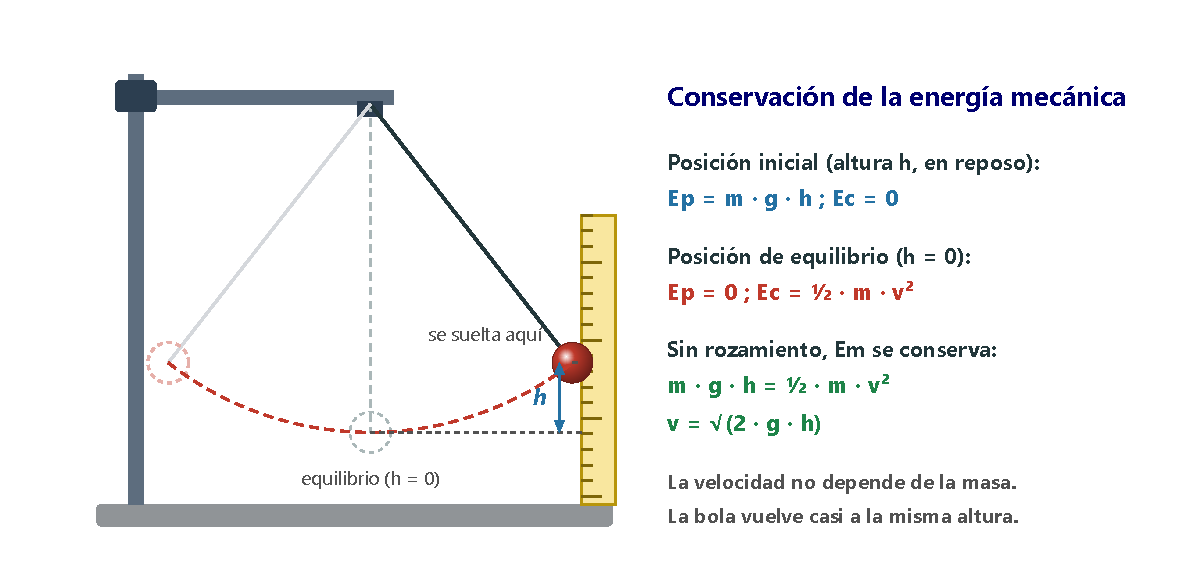
\includegraphics[width=0.9\textwidth]{images/UD11/pendulo_energia}
    \caption{Montaje del péndulo para comprobar la conservación de la energía mecánica.}
    \label{fig:pendulo_energia}
\end{figure}

\noindent\begin{minipage}[t]{0.53\textwidth}
    \textbf{Objetivos}
    \begin{itemize}
        \item Trabajar con materiales e instrumentos del laboratorio de Física.
        \item Valorar el trabajo experimental sistemático.
        \item Medir longitudes con los instrumentos adecuados.
        \item Comprobar el principio de conservación de la energía mecánica.
    \end{itemize}
\end{minipage}\hfill
\begin{minipage}[t]{0.43\textwidth}
    \textbf{Material}
    \begin{itemize}
        \item Un soporte con una pinza metálica y una nuez.
        \item Una esfera de metal y un hilo.
        \item Una regla.
    \end{itemize}
\end{minipage}

\medskip

\textbf{Procedimiento}
\begin{enumerate}[label=\numberballgreen]
    \item Monta el péndulo como en la figura~\ref{fig:pendulo_energia} y sujeta la bola al extremo del hilo.
    \item Coloca la regla en vertical, con el cero (\(h = 0\)) a la altura de la bola en la posición de equilibrio.
    \item Separa la bola hasta que esté a una altura \(h\) que puedas medir con la regla y suéltala sin empujarla.
    \item Observa si, después de una oscilación completa, la bola vuelve a la misma altura.
\end{enumerate}

\begin{exercise}
    Responde a estas preguntas sobre la práctica:
    \begin{enumerate}[label=\alph*)]
        \item ¿Qué tipo de energía tiene la bola en la posición inicial, a la altura \(h\)? ¿Y al pasar por la posición de equilibrio? Explica con un esquema las transformaciones de energía.
        \item Demuestra que la velocidad de la bola en la posición de equilibrio es \(v = \sqrt{2 \cdot g \cdot h}\). ¿Hace falta conocer su masa?
        \item ¿Con qué velocidad pasa por la posición de equilibrio si se suelta desde \qty{20}{\cm}?
        \item Si la bola tiene \qty{25}{\gram}, completa la tabla en tu cuaderno:
        \begin{center}
            % --- tabla antigua ---
            % \begin{tblr}{colspec={cccc}, hlines, vlines, row{1}={bg=ocre!85, fg=white, font=\bfseries\small}, cells={font=\small}}
                % \(h\) (cm) & \(E_p\) inicial (J) & \(E_c\) en el equilibrio (J) & \(v\) en el equilibrio (m/s) \\
                % 15 & \ldots & \ldots & \ldots \\
                % 20 & \ldots & \ldots & \ldots \\
                % 25 & \ldots & \ldots & \ldots \\
                % 30 & \ldots & \ldots & \ldots \\
            % \end{tblr}
            % --- tabla nueva ---
            {\small
            \begin{tabular}{@{}cccc@{}}
                \toprule
                \textbf{\(h\) (cm)} & \textbf{\(E_p\) inicial (J)} & \textbf{\(E_c\) en el equilibrio (J)} & \textbf{\(v\) en el equilibrio (m/s)} \\
                \midrule
                15 & \ldots & \ldots & \ldots \\[3pt]
                20 & \ldots & \ldots & \ldots \\[3pt]
                25 & \ldots & \ldots & \ldots \\[3pt]
                30 & \ldots & \ldots & \ldots \\
                \bottomrule
            \end{tabular}
            }
        \end{center}
        \item ¿Vuelve la bola exactamente a la misma altura? ¿Por qué?
    \end{enumerate}
    \begin{solu}
        a) Al principio, solo \textcolor{red}{energía potencial}; en la posición de equilibrio, solo \textcolor{red}{energía cinética}. Mientras baja, la potencial se transforma en cinética, y al subir por el otro lado ocurre al revés.
        b) \(m \cdot g \cdot h = \frac{1}{2} \cdot m \cdot v^2 \Rightarrow v = \sqrt{2 \cdot g \cdot h}\): la masa se simplifica, así que \textcolor{red}{no hace falta conocerla}.
        c) \(v = \sqrt{2 \cdot \num{9.8} \cdot \num{0.20}} = \textcolor{red}{\qty{1.98}{\m\per\s}}\).
        d) Con \(E_p = \num{0.025} \cdot \num{9.8} \cdot h\) y \(E_c = E_p\): \qty{15}{\cm}: \qty{0.037}{\joule}, \qty{1.71}{\m\per\s}; \qty{20}{\cm}: \qty{0.049}{\joule}, \qty{1.98}{\m\per\s}; \qty{25}{\cm}: \qty{0.061}{\joule}, \qty{2.21}{\m\per\s}; \qty{30}{\cm}: \qty{0.074}{\joule}, \qty{2.42}{\m\per\s}.
        e) Llega \textcolor{red}{casi} a la misma altura, pero un poco más abajo: el \textcolor{red}{rozamiento con el aire} transforma una pequeña parte de la energía mecánica en térmica, y tras muchas oscilaciones el péndulo se para.
    \end{solu}
\end{exercise}

%========================================================================================
\section[Unidad 12. Calor específico]{Unidad 12. Medida de la capacidad calorífica específica}
%========================================================================================
% (sacado del final de UD12_calor.tex)

La capacidad calorífica específica es una propiedad característica: sustancias distintas suben su temperatura de forma diferente cuando reciben la misma cantidad de calor. En esta práctica la mediremos con un calorímetro, aplicando el balance de energía:
\[ m_1 \cdot c_1 \cdot (T_1 - T_{\text{eq}}) = m_2 \cdot c_2 \cdot (T_{\text{eq}} - T_2) \]

\begin{figure}[H]
    \centering
    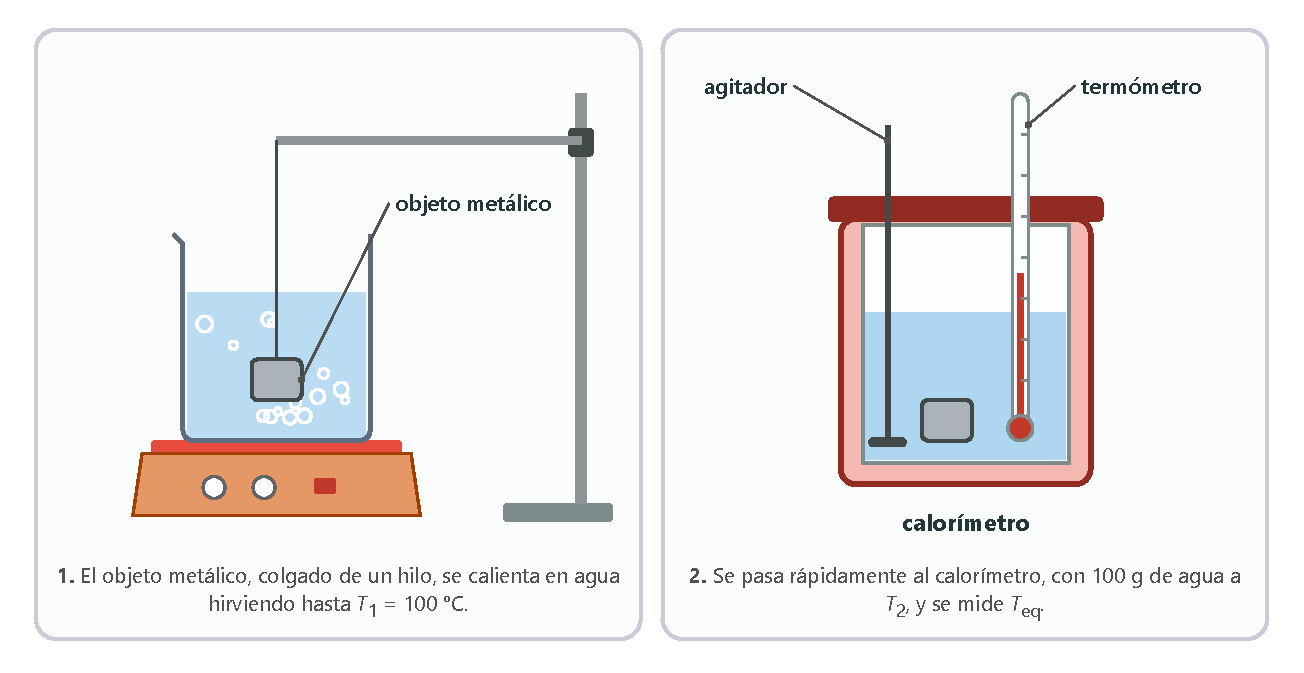
\includegraphics[width=\textwidth]{images/UD12/practica_calor_especifico}
    \caption{Montaje para medir la capacidad calorífica específica de un metal.}
    \label{fig:practica_calor_especifico}
\end{figure}

\noindent\begin{minipage}[t]{0.53\textwidth}
    \textbf{Objetivos}
    \begin{itemize}
        \item Trabajar con materiales e instrumentos del laboratorio de Física.
        \item Valorar el trabajo experimental sistemático.
        \item Medir masas y temperaturas con los instrumentos adecuados.
        \item Medir la capacidad calorífica específica de un objeto metálico.
    \end{itemize}
\end{minipage}\hfill
\begin{minipage}[t]{0.43\textwidth}
    \textbf{Material}
    \begin{itemize}
        \item Un vaso de precipitados y un hornillo.
        \item Un calorímetro y un termómetro.
        \item \qty{100}{\gram} de agua.
        \item Un objeto metálico de masa conocida y un hilo.
        \item Un soporte con pinza.
    \end{itemize}
\end{minipage}

\medskip

\textbf{Procedimiento}
\begin{enumerate}[label=\numberballgreen]
    \item Ata el objeto metálico a un hilo y sumérgelo en un vaso de precipitados con agua. Calienta hasta que el agua hierva: el objeto estará a la temperatura de ebullición, \(T_1\).
    \item Mientras el agua hierve, echa en el calorímetro \qty{100}{\gram} de agua a temperatura ambiente. Tápalo, introduce el termómetro, espera unos minutos y anota su temperatura, \(T_2\).
    \item Cuando el agua del vaso lleve un rato hirviendo, saca el objeto tirando del hilo e introdúcelo rápidamente en el calorímetro. Tápalo y agita suavemente con la varilla.
    \item Anota la temperatura máxima que marca el termómetro: es la temperatura de equilibrio, \(T_{\text{eq}}\).
    \item Repite el experimento varias veces y calcula el valor medio de \(T_{\text{eq}}\).
\end{enumerate}

\begin{exercise}
    Un grupo de alumnos ha usado un objeto metálico de \qty{80}{\gram} y \qty{100}{\gram} de agua a \(T_2 = \qty{20.0}{\degreeCelsius}\). Estas son sus medidas:
    \begin{center}
        % --- tabla antigua ---
        % \begin{tblr}{colspec={cccccc}, hlines, vlines, row{1}={bg=ocre!85, fg=white, font=\bfseries}}
            % Experiencia & 1 & 2 & 3 & 4 & 5 \\
            % \(T_{\text{eq}}\) (\unit{\degreeCelsius}) & \num{31.6} & \num{32.1} & \num{31.8} & \num{31.5} & \num{32.0} \\
        % \end{tblr}
        % --- tabla nueva ---
        \begin{tabular}{@{}cccccc@{}}
            \toprule
            \textbf{Experiencia} & \textbf{1} & \textbf{2} & \textbf{3} & \textbf{4} & \textbf{5} \\
            \midrule
            \(T_{\text{eq}}\) (\unit{\degreeCelsius}) & \num{31.6} & \num{32.1} & \num{31.8} & \num{31.5} & \num{32.0} \\
            \bottomrule
        \end{tabular}
    \end{center}
    \begin{enumerate}[label=\alph*)]
        \item ¿Qué temperatura, \(T_1\), tiene el objeto cuando lo sacas del vaso?
        \item Calcula el valor medio de la temperatura de equilibrio.
        \item Calcula la capacidad calorífica específica del metal.
        \item ¿De qué metal puede estar hecho el objeto? ¿Por qué el resultado no coincide exactamente con el de la tabla?
    \end{enumerate}
    \begin{solu}
        a) Ha alcanzado el equilibrio térmico con el agua hirviendo, así que está a \textcolor{red}{\qty{100}{\degreeCelsius}} (aproximadamente; depende de la presión atmosférica).
        b) \(T_{\text{eq}} = \dfrac{\num{31.6} + \num{32.1} + \num{31.8} + \num{31.5} + \num{32.0}}{5} = \textcolor{red}{\qty{31.8}{\degreeCelsius}}\).
        c) \(\num{0.080} \cdot c \cdot (100 - \num{31.8}) = \num{0.100} \cdot 4180 \cdot (\num{31.8} - \num{20.0}) \Rightarrow \num{5.456} \cdot c = \num{4932.4}\)
        \[ c = \textcolor{red}{\qty{904}{\cunit}} \]
        d) Probablemente es \textcolor{red}{aluminio} (\qty{910}{\cunit}). La diferencia se debe a los errores de medida, a la energía que se pierde al trasladar el objeto y a que no hemos tenido en cuenta el calor que absorbe el propio calorímetro.
    \end{solu}
\end{exercise}

%========================================================================================
\section{Unidad 13. La resonancia acústica}
%========================================================================================
% (sacado del final de UD13_luz_sonido.tex)

Todos los objetos, y también las columnas de aire encerradas en un tubo, tienen una o varias \textbf{frecuencias naturales} de vibración. Si les llega una onda que vibra justo con una de esas frecuencias, empiezan a vibrar con una amplitud cada vez mayor y el sonido se refuerza. Este fenómeno se llama \textbf{resonancia}.

\begin{figure}[H]
    \centering
    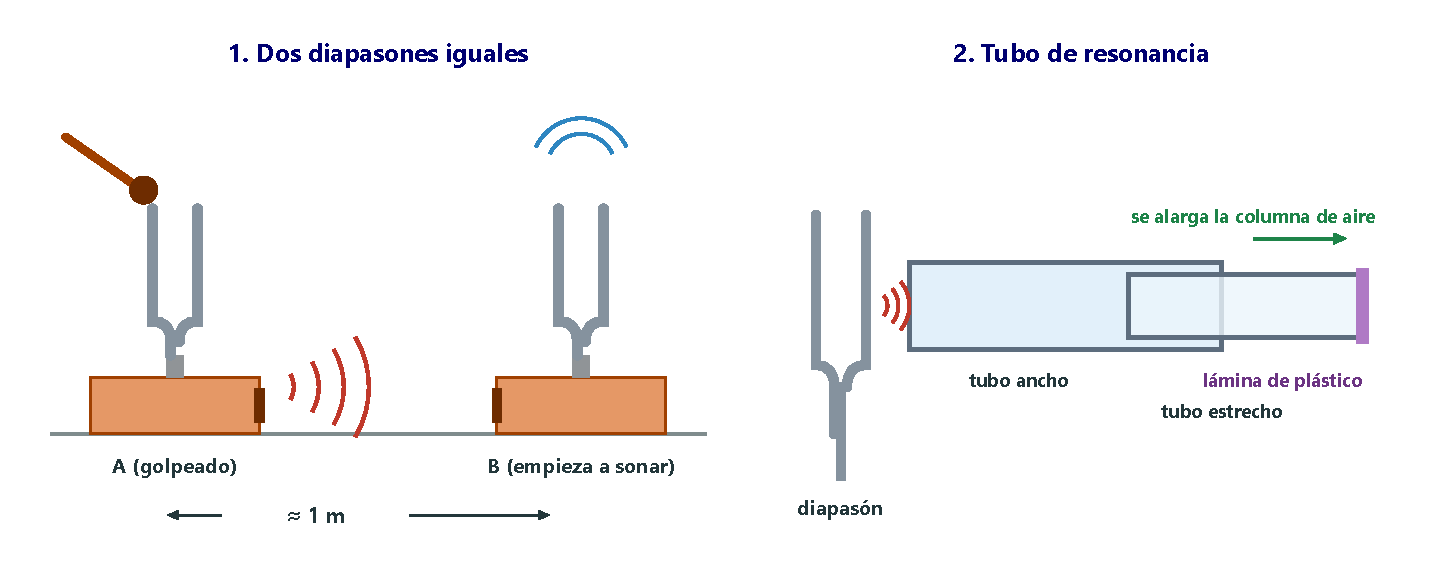
\includegraphics[width=\textwidth]{images/UD13/practica_resonancia}
    \caption{Montajes de la práctica: dos diapasones iguales enfrentados (1) y un tubo de resonancia de longitud variable (2).}
    \label{fig:practica_resonancia}
\end{figure}

\noindent\begin{minipage}[t]{0.53\textwidth}
    \textbf{Objetivos}
    \begin{itemize}
        \item Comprobar experimentalmente la resonancia acústica en un tubo.
        \item Comprobar que un diapasón hace vibrar por resonancia a otro igual.
        \item Trabajar con materiales del laboratorio de Física.
        \item Valorar la importancia del trabajo experimental.
    \end{itemize}
\end{minipage}\hfill
\begin{minipage}[t]{0.43\textwidth}
    \textbf{Material}
    \begin{itemize}
        \item Dos tubos de plástico rígido que encajen uno dentro del otro.
        \item Dos diapasones de la misma frecuencia con caja de resonancia.
        \item Un martillo de goma y una regla.
        \item Una lámina de plástico.
    \end{itemize}
\end{minipage}

\medskip

\textbf{Procedimiento}
\begin{enumerate}[label=\numberballgreen]
    \item Coloca los dos diapasones a \qty{1}{\m} de distancia, con las aberturas de sus cajas enfrentadas. Golpea uno con el martillo de goma y escucha. Al cabo de unos segundos, tócalo con los dedos para que deje de sonar.
    \item Coge el otro diapasón por la parte trasera de su caja y acércalo al oído: oirás que está sonando, aunque nadie lo ha golpeado. La vibración ha pasado de un diapasón a otro por resonancia.
    \item Introduce el tubo estrecho en el ancho y tapa con la lámina de plástico el extremo libre del tubo estrecho. Golpea un diapasón (sin caja) y colócalo delante de la boca del tubo ancho.
    \item Sin dejar de escuchar, desliza el tubo estrecho hacia fuera para alargar la columna de aire. Anota con la regla la longitud para la que el sonido se oye con más fuerza. Repite la experiencia varias veces.
\end{enumerate}

\begin{exercise}
    Explica cómo se transmite el sonido de un diapasón al otro.
    \begin{solu}
        El diapasón golpeado hace vibrar el aire, y la onda sonora llega al segundo diapasón. Como los dos tienen la \textcolor{red}{misma frecuencia natural}, el segundo empieza a vibrar cada vez con más amplitud: es la \textcolor{red}{resonancia}.
    \end{solu}
\end{exercise}

\begin{exercise}
    A partir de la experiencia, responde:
    \begin{enumerate}[label=\alph*)]
        \item ¿Habrías conseguido el mismo efecto con dos diapasones de distinta frecuencia?
        \item ¿Crees que la resonancia en tubos está relacionada con el sonido de algunos instrumentos musicales?
        \item ¿Qué relación puede haber entre la longitud del tubo y que el sonido sea más agudo o más grave?
    \end{enumerate}
    \begin{solu}
        a) \textcolor{red}{No}: solo hay resonancia si la frecuencia de la onda coincide con la frecuencia natural del segundo diapasón.
        b) \textcolor{red}{Sí}: en los instrumentos de viento (flauta, clarinete, trompeta, órgano) la columna de aire del tubo resuena y refuerza ciertas notas; en los de cuerda, la caja de resonancia amplifica el sonido de las cuerdas.
        c) Cuanto \textcolor{red}{más largo es el tubo, más grave} es el sonido con el que resuena (menor frecuencia); los tubos cortos resuenan con sonidos agudos. Por eso los tubos de un órgano son de distintas longitudes.
    \end{solu}
\end{exercise}

\begin{exercise}
    En un tubo cerrado por un extremo, el primer refuerzo del sonido se produce cuando la longitud de la columna de aire es la cuarta parte de la longitud de onda, \(L = \lambda/4\). Un grupo usa un diapasón de \qty{440}{\hertz} y oye el primer refuerzo con \(L = \qty{19.5}{\cm}\). Calcula la velocidad del sonido que se deduce de su medida.
    \begin{solu}
        \(\lambda = 4L = 4 \cdot \num{0.195} = \qty{0.78}{\m}\). \(v = \lambda \cdot f = \num{0.78} \cdot 440 = \textcolor{red}{\qty{343}{\m\per\s}}\), muy próxima al valor tabulado (\(\approx \qty{340}{\m\per\s}\)).
    \end{solu}
\end{exercise}


%------------------------------------------------


    \chapterimage{images/portada_cabeceras/cabecera_general}
    \chapter{Situaciones de aprendizaje}

    % Situaciones de aprendizaje de cada unidad.
% Se incluye en el anexo de Libro_4_ESO_ES.tex. Ordenado por unidades.

%========================================================================================
\section[Unidad 1. El pensamiento científico]{Unidad 1. La evolución del pensamiento científico}
%========================================================================================
% (sacado del final de UD1_Trabajo_cientifico.tex)

Todo lo que sucede en la naturaleza se puede organizar y explicar con unas pocas leyes: fenómenos aparentemente distintos, como la caída de una manzana y la órbita de la Luna, se explican con la ley de gravitación universal. El conocimiento científico ha evolucionado a lo largo de la historia y, a menudo, ha estado influido por el contexto político, económico o religioso. La ciencia moderna es fruto del trabajo de personas como Galileo, Bacon, Descartes o Newton, que usaron el método científico: un procedimiento experimental, riguroso y cuantitativo.

\begin{marker}
    \textbf{Reto:} investigar la evolución del conocimiento científico sobre un tema, relacionando los descubrimientos con sus protagonistas y con su contexto histórico, y elaborar una \textbf{línea del tiempo} y una presentación.
\end{marker}

Temas posibles: el origen del universo y los métodos para observarlo; el movimiento de estrellas, planetas y satélites; la naturaleza de la luz; la estructura atómica; la radiactividad; la química del carbono; la meteorología; el Sistema Internacional de unidades; las máquinas térmicas; el calentamiento global y el cambio climático.

\begin{enumerate}[label=\numberballred]
    \item \textbf{Grupos y tema.} En pequeños grupos, elegid un tema distinto para cada grupo.
    \item \textbf{Investigación.} Investigad las circunstancias históricas que impulsaron esos avances (soluciones de ingeniería, nuevos materiales, descubrimientos previos) y las posibles resistencias sociales o políticas.
    \item \textbf{Línea del tiempo.} Elegid un modelo y situad en ella las etapas (investigaciones, descubrimientos, teorías, leyes, publicaciones, controversias), sus protagonistas y los sucesos históricos de cada momento.
    \item \textbf{Presentación.} Preparad una presentación sobre los científicos y científicas que contribuyeron al tema, con sus datos biográficos más importantes e ilustraciones (citando su procedencia).
    \item \textbf{Comunicación.} Presentad la línea del tiempo en clase, comparad hechos ocurridos en la misma época en los distintos temas y publicad los trabajos en la revista del departamento.
\end{enumerate}

%========================================================================================
\section{Unidad 2. La historia del átomo en una línea del tiempo}
%========================================================================================
% (sacado del final de UD_2_el_atomo_tp.tex)

En 1869, el químico ruso \textbf{Dmitri Mendeléiev} ordenó los 63 elementos conocidos por masa atómica creciente y se dio cuenta de que las propiedades se repetían periódicamente. Colocó juntos los elementos parecidos y, cuando un elemento no encajaba, cambió el orden o \textbf{dejó un hueco} para un elemento aún desconocido, cuyas propiedades predijo. Así ocurrió con el galio (descubierto en 1875) y el germanio (1886). Entre 1894 y 1898, \textbf{William Ramsay} descubrió los gases nobles, que no estaban previstos, y los colocó en una nueva columna: el actual grupo 18.

\begin{marker}
    \textbf{Reto:} diseñad en grupos una \textbf{línea del tiempo} que recoja los principales descubrimientos que llevaron a los distintos modelos atómicos, los relacionados con la radiactividad y las fechas de descubrimiento de algunos elementos químicos.
\end{marker}

\begin{enumerate}[label=\numberballred]
    \item \textbf{Investigación.} Repartid el trabajo en grupos de dos o tres personas sin que se repitan los temas. Anotad las fechas que aparecen en la unidad y ampliadlas con modelos más modernos, la radiactividad y sus aplicaciones, y el descubrimiento de elementos. Identificad a los científicos y científicas protagonistas.
    \item \textbf{Fichas.} Diseñad una ficha común para recoger de forma homogénea cada acontecimiento (fecha, protagonista, descubrimiento, importancia, imagen). Añadid algún hecho histórico que sirva de referencia de cada época.
    \item \textbf{Construcción.} Elegid un formato (mural o herramienta digital) adaptado al lugar donde se expondrá y acompañad la información con ilustraciones. Haced un reportaje fotográfico o en vídeo del proceso.
    \item \textbf{Comunicación.} Exponed la línea del tiempo en el aula o en el centro, explicadla a compañeros de otros cursos y publicadla en la revista digital, el blog de la asignatura o la web del departamento.
\end{enumerate}

%========================================================================================
\section{Unidad 3. Materiales para la ingeniería y el deporte}
%========================================================================================
% (sacado del final de UD3_enlace_quimico.tex)

Los deportistas baten sus propias marcas una y otra vez. En buena parte se debe a los \textbf{nuevos materiales}: más flexibles y ligeros, pero también más fuertes y resistentes. La madera, el hierro o el cuero han ido dejando paso a compuestos químicos de alta tecnología. Para saltar más alto, nadar más rápido, bucear más hondo o correr más deprisa hacen falta cuerdas más ligeras, trajes protectores, zapatillas especiales, raquetas, pelotas o palos de golf más ligeros, fuertes y elásticos. Muchas veces, el resultado de un atleta depende de la calidad tecnológica de su equipamiento: la velocidad es, en definitiva, una cuestión de física y de química.

\begin{marker}
    \textbf{Reto:} investigad los materiales (elementos y compuestos) que se usan en la ingeniería y la construcción, y los nuevos materiales de las equipaciones e instrumentos deportivos. Preparad unas \textbf{fichas identificativas} y una \textbf{exposición física o virtual}. Podéis hacerlo en colaboración con el departamento de Educación Física.
\end{marker}

\begin{enumerate}[label=\numberballred]
    \item \textbf{Investigación.} Buscad información sobre los materiales que se usan en ingeniería, construcción y edificación. No olvidéis las nuevas aleaciones metálicas ni las formas alotrópicas del carbono (fibra de carbono, grafeno, nanotubos).
    \item \textbf{Fichas.} Diseñad una ficha común que recoja las características de los materiales de las equipaciones deportivas y de los instrumentos de cada deporte (tipo de sustancia, enlace, propiedades, ventajas). Si es posible, comparadlos con los que se usaban hace unas décadas.
    \item \textbf{Análisis.} Elegid un deporte y comparad sus marcas de hace 20 o 30 años con las actuales. ¿Puede estar relacionada la mejora con el uso de nuevos materiales?
    \item \textbf{Elaboración.} Haced una lista de materiales de ingeniería y construcción y sus aplicaciones, acompañada de fotografías o ilustraciones.
    \item \textbf{Comunicación.} Preparad en clase una presentación, a modo de reportaje, sobre la evolución de los materiales deportivos y su relación con la evolución de las marcas, y exponedla en el centro o en la web del departamento.
\end{enumerate}

%========================================================================================
\section[Unidad 4. Compuestos de carbono y plásticos]{Unidad 4. Compuestos de carbono de interés industrial y biológico. Reciclaje de plásticos}
%========================================================================================
% (sacado del final de UD4_organica.tex)

Se conocen más de diez millones de compuestos del carbono, y gran parte de la industria química se dedica a fabricar plásticos. Pero sus residuos son un problema: los envases de un solo uso son uno de los elementos más contaminantes. En 2022, la Comisión Europea propuso nuevas normas porque cada europeo genera unos \qty{180}{\kg} de residuos de envases al año, y sin medidas los residuos de envases de plástico podrían aumentar un \qty{46}{\percent} para 2030. Entre las medidas están prohibir algunos envases de un solo uso (para comer y beber en los restaurantes, para frutas y verduras o los envases en miniatura de los hoteles), exigir que todos los envases sean reciclables y crear sistemas de devolución de botellas y latas. El objetivo es \textbf{prevenir} la generación de envases, \textbf{impulsar} un reciclado de calidad y \textbf{reducir} el consumo de recursos naturales.

\begin{marker}
    \textbf{Reto:} investigar las propiedades y aplicaciones de un compuesto de carbono cercano y analizar el consumo de envases no reutilizables en el centro, con una campaña de concienciación (eslóganes y póster).
\end{marker}

\begin{enumerate}[label=\numberballred]
    \item \textbf{Grupos y compuesto.} En pequeños grupos, elegid un compuesto de carbono (etanol, gas natural, neopreno, aceites, glucosa, PVC, vitaminas, jabón, caucho, percloroetileno\ldots), procurando que no se repitan entre los grupos.
    \item \textbf{Investigación.} Buscad si es natural o artificial, sus propiedades físicas y químicas, sus aplicaciones (domésticas, clínicas, industriales), los problemas ambientales que puede causar y las normas que regulan su uso.
    \item \textbf{Ficha común.} Diseñad entre todos un modelo de ficha: nombre, fórmula, masa molecular, puntos de fusión y ebullición, aplicaciones, importancia biológica y problemas para la salud o el medio ambiente. Elaborad con las fichas un póster mural o una infografía.
    \item \textbf{Los plásticos del centro.} Analizad qué envases de plástico se generan en el centro, comprobad si se depositan en el contenedor adecuado y redactad un informe sobre cómo reducirlos o sustituirlos por envases reutilizables.
    \item \textbf{Campaña.} Diseñad pósteres con eslóganes sobre el uso excesivo de plásticos y su efecto en el medio ambiente, y publicad los resultados en la revista digital del departamento.
    \item \textbf{Evaluación.} Al cabo de un tiempo, comprobad si han disminuido los residuos plásticos del centro (podéis hacer también una encuesta al alumnado de otros grupos).
\end{enumerate}

\begin{exercise}
    El PVC (cloruro de polivinilo) se obtiene por polimerización del cloruro de vinilo, \ch{CH2=CHCl}. a) Calcula la masa molecular del monómero y su porcentaje de cloro. b) ¿Qué tipo de plástico es el PVC según su comportamiento con el calor? c) ¿Por qué es un problema que los plásticos sean tan estables?
    \begin{solu}
        a) \ch{C2H3Cl}: \(M = 24 + 3 + \num{35.5} = \textcolor{red}{\num{62.5}}\); \% Cl \(= \dfrac{\num{35.5}}{\num{62.5}} \cdot 100 = \textcolor{red}{\qty{56.8}{\percent}}\).
        b) Es un \textcolor{red}{termoplástico}: se reblandece al calentarlo y puede moldearse y reciclarse.
        c) Porque \textcolor{red}{tardan cientos de años en degradarse}: se acumulan en vertederos, ríos y océanos, y se fragmentan en microplásticos que entran en las cadenas alimentarias.
    \end{solu}
\end{exercise}

%========================================================================================
\section{Unidad 5. La atmósfera, un sistema material que proteger}
%========================================================================================
% (sacado del final de UD5_Sistema_materiales.tex)

La contaminación atmosférica se debe a la emisión de gases y partículas procedentes de la actividad humana y de fuentes naturales, como los volcanes. Algunos contaminantes que afectan a nuestra salud y a los ecosistemas son el dióxido de azufre (\ch{SO2}), el trióxido de azufre (\ch{SO3}), los óxidos de nitrógeno (\ch{NO2}, \ch{N2O}\ldots), el monóxido de carbono (\ch{CO}), el dióxido de carbono (\ch{CO2}) y el ozono que se forma a baja altura. También contaminan las \textbf{partículas en suspensión}: polvo, metales y compuestos orgánicos e inorgánicos. El clima influye en cómo se dispersan y transportan estos contaminantes.

\begin{marker}
    \textbf{Reto:} evaluad la calidad del aire de vuestro entorno en distintas épocas del año y redactad un \textbf{decálogo de buenas prácticas} para reducir los contaminantes atmosféricos.
\end{marker}

\begin{enumerate}[label=\numberballred]
    \item \textbf{La capa inicial de la atmósfera.} El \qty{95}{\percent} de la masa del aire (unos \qty{5.1e18}{\kg}) está en los primeros \qty{11}{\km}. Investigad en pequeños grupos qué gases la componen y en qué proporción.
    \item \textbf{Datos de calidad del aire.} Con alguna aplicación o web de calidad del aire, anotad durante varias semanas, en distintas épocas del año, la calidad del aire de vuestra localidad y el contaminante principal. ¿Coinciden esos gases con los de la composición del aire?
    \item \textbf{Código de colores.} Analizad qué significan los colores (verde, amarillo, rojo\ldots) con que se indica la calidad del aire.
    \item \textbf{Zonas de bajas emisiones.} Averiguad si en vuestra localidad hay zonas de bajas emisiones (ZBE), qué vehículos pueden entrar y por qué. Situadlas en un plano y comprobad si en ellas la calidad del aire es mejor.
    \item \textbf{Comunicación.} Representad los datos en tablas y gráficas y publicad el análisis en el centro o en la revista digital del departamento.
    \item \textbf{Decálogo.} En grupos, redactad buenas prácticas individuales y colectivas para reducir la contaminación del aire. Ponedlas en común, elaborad un único decálogo de la clase y exponedlo en el aula.
\end{enumerate}

%========================================================================================
\section{Unidad 6. Las combustiones en nuestra vida diaria}
%========================================================================================
% (sacado del final de UD6_reacciones_quimicas.tex)

Piensa en cualquier producto que consumes: hay que fabricarlo, envasarlo, almacenarlo, transportarlo hasta la tienda, anunciarlo y, al final, deshacerse de él. Todo ello genera residuos y consume mucha energía, buena parte procedente de combustiones. Comprar productos locales reduce las distancias del transporte y, con ello, el consumo de energía y la emisión de gases de efecto invernadero. Además, el comercio de proximidad ayuda a que las ciudades sean más sostenibles. Aunque las grandes decisiones corresponden a los gobiernos, los ODS solo se alcanzarán con acciones individuales comprometidas.

\begin{marker}
    \textbf{Reto:} estudiad el impacto medioambiental de las combustiones que usamos para obtener energía en casa y en la industria, y realizad una \textbf{campaña informativa} sobre los efectos de quemar combustibles fósiles, entre ellos la lluvia ácida y el incremento del efecto invernadero.
\end{marker}

\begin{enumerate}[label=\numberballred]
    \item \textbf{Investigación.} Averiguad cómo se usan las combustiones para producir electricidad y cómo se emplea esa energía en el transporte, en los hogares y en los lugares de trabajo, estudio y ocio.
    \item \textbf{Transporte de mercancías.} Buscad datos sobre las combustiones necesarias para transportar personas y mercancías, y para fabricar materias primas y bienes de consumo a veces muy lejos del lugar donde se usan.
    \item \textbf{Análisis.} Comparad el doble impacto (producción y transporte) de los productos lejanos con el de los productos de proximidad.
    \item \textbf{Póster 1.} Mostrad que somos responsables de la contaminación que producimos, tanto con el transporte como con la energía doméstica, incluyendo la que generan los productos que vienen de lejos.
    \item \textbf{Póster 2.} Explicad cómo se produce la electricidad en una central térmica y qué combustible usa. Recordad que esa energía alimenta todos los aparatos eléctricos, incluidos los vehículos eléctricos.
    \item \textbf{Decálogo.} Redactad buenas prácticas individuales y colectivas para reducir el impacto de los combustibles fósiles y publicadlas en la revista del centro o del departamento.
    \item \textbf{Comunicación.} Exponed la campaña a toda la comunidad educativa, con los pósteres como apoyo.
\end{enumerate}

%========================================================================================
\section{Unidad 7. El movimiento en el deporte}
%========================================================================================
% (sacado del final de UD7_movimientos_rectilineos.tex)

En el deporte hay que medir distancias en los campos de juego, en los saltos y en los lanzamientos, y tiempos en las carreras a pie o de patinaje. Muchas medidas se hacen fuera de la pista, en laboratorios que prueban los materiales. En la Fórmula 1 se miden longitudes, tiempos y masas para cumplir el reglamento, y en la natación artística se controlan la temperatura y la profundidad del agua. Para homologar un récord, las medidas deben hacerse con instrumentos certificados por un laboratorio reconocido.

\begin{marker}
    \textbf{Reto:} investigad cómo se miden las magnitudes del movimiento (sistema de referencia, espacio, tiempo, velocidad, aceleración) en distintos deportes y elaborad una \textbf{infografía} o un \textbf{pódcast} con los resultados.
\end{marker}

\begin{enumerate}[label=\numberballred]
    \item \textbf{Análisis.} En grupos de hasta cinco personas, haced una lista de deportes en los que lo más importante sea la velocidad y otra en los que lo sea la resistencia. Cada miembro elige una disciplina diferente de la primera lista.
    \item \textbf{Investigación.} Buscad cómo se establece el sistema de referencia (salida y llegada), cómo se mide el espacio recorrido y el tiempo, y qué se necesita para que una marca sea homologable.
    \item \textbf{Récords.} Consultad las marcas mundiales actuales de vuestra disciplina y cómo han evolucionado en las dos últimas décadas.
    \item \textbf{Nuestra carrera.} Con el profesorado de Educación Física, organizad una carrera de \qty{100}{\m} con toda la clase: calculad la velocidad media de cada participante y analizad las fases de la carrera (salida, aceleración, velocidad máxima y resistencia), por ejemplo midiendo los tiempos de paso cada \qty{20}{\m}.
    \item \textbf{Ficha común.} Diseñad entre toda la clase una ficha con la misma estructura para recoger la información y cumplimentadla.
    \item \textbf{Infografía o pódcast.} Elaborad una infografía o un pódcast que resuma vuestra investigación, y un informe personal con los resultados de la carrera.
    \item \textbf{Comunicación.} Presentad vuestro trabajo al resto de la clase y debatid sobre los métodos de medida en los deportes de velocidad.
\end{enumerate}

%========================================================================================
\section{Unidad 8. El rozamiento y la acción-reacción en la vida diaria}
%========================================================================================
% (sacado del final de UD8_fuerzas.tex)

En la final del Mundial de natación de Roma, el 30 de julio de 2009, el brasileño César Cielo tocó la pared en \qty{46.91}{\s} en los \qty{100}{\m} libres, ayudado por un bañador de poliuretano que reducía el rozamiento con el agua y lo hacía flotar mejor. Esos bañadores se prohibieron en 2010 y, durante años, ningún nadador con bañador de tela consiguió acercarse a aquella marca. En agosto de 2022, el rumano David Popovici la batió con \qty{46.86}{\s}: rotaba el tronco y clavaba las manos en el agua, ofreciendo muy poca superficie al rozamiento.

\begin{marker}
    \textbf{Reto:} identificad e interpretad las fuerzas de rozamiento y las fuerzas de acción y reacción en situaciones cotidianas y deportivas, y preparad una \textbf{presentación}, una \textbf{infografía} o un \textbf{mural}.
\end{marker}

\begin{enumerate}[label=\numberballred]
    \item \textbf{Grupos.} Formad grupos de hasta cinco personas.
    \item \textbf{Situaciones.} Buscad situaciones de la vida diaria y del deporte en las que aparezcan fuerzas de rozamiento y de acción y reacción: caminar sobre distintos terrenos, borrar la pizarra, arrastrar un objeto, saltar desde una barca o un monopatín, nadar\ldots
    \item \textbf{Análisis.} Identificad en cada caso las fuerzas de rozamiento y las parejas de acción y reacción, y dibujadlas.
    \item \textbf{Los bañadores.} ¿Por qué se conseguían mejores marcas con los bañadores de poliuretano que con los de tela? ¿Creéis que estuvo justificada su prohibición?
    \item \textbf{Técnica.} Analizad cómo nadaba Popovici para ser más rápido y eficaz.
    \item \textbf{Puesta en común.} Haced una lista con todas las situaciones estudiadas para que no se repitan entre grupos, y comprobad cuántas se aprovechan para facilitar el movimiento, sobre todo en el deporte.
    \item \textbf{Elaboración.} Buscad fotografías o vídeos (citando su autoría) y preparad la presentación, la infografía o el mural con al menos cuatro situaciones.
    \item \textbf{Comunicación.} Presentad vuestro trabajo a la clase o difundidlo con los medios del centro.
\end{enumerate}

%========================================================================================
\section[Unidad 9. El universo y la gravedad]{Unidad 9. Conocimiento del universo y la fuerza gravitatoria}
%========================================================================================
% (sacado del final de UD9_movimiento_circular.tex)

La gravedad influye en el desarrollo de las plantas en la Tierra: las raíces crecen hacia abajo y los tallos hacia arriba. En el experimento \emph{Plant Gravity Sensing}, realizado en la Estación Espacial Internacional, se cultivaron semillas de \emph{Arabidopsis} (una planta muy usada en investigación) en microgravedad. Sus raíces crecieron enredadas en la malla de cultivo, de forma muy distinta a las cultivadas en la Tierra. Entender cómo «sienten» las plantas la gravedad podría ayudar a obtener nuevas variedades de cultivos.

Investigaciones como esta son posibles gracias a siglos de avances en el conocimiento del universo y de la gravedad, desde Copérnico y Kepler hasta los satélites y las estaciones espaciales.

\begin{marker}
    \textbf{Reto:} construid una \textbf{línea del tiempo} con la evolución del conocimiento del universo y de la fuerza gravitatoria, de los métodos de observación del universo y de la navegación espacial, junto con sus protagonistas más destacados.
\end{marker}

\begin{enumerate}[label=\numberballred]
    \item \textbf{Grupos y tema.} En grupos de hasta cinco personas, elegid uno de estos aspectos: evolución del conocimiento del universo; evolución de las teorías sobre la gravedad; métodos de observación del universo; la navegación espacial\ldots{} Procurad que no haya más de dos grupos con el mismo aspecto.
    \item \textbf{Investigación.} Ampliad la información sobre los experimentos que se hacen en la Estación Espacial Internacional y cómo contribuyen al avance de la ciencia (podéis consultar la web de la ESA).
    \item \textbf{Ficha común.} Diseñad entre todos un modelo de ficha para recoger la información de cada hecho científico en su contexto histórico: fecha, protagonistas, aportación, contexto y fuentes.
    \item \textbf{Elaboración.} Decidid dónde vais a exponer la línea del tiempo y elegid las dimensiones adecuadas. Buscad un modelo o diseñad el vuestro e incluid ilustraciones de los hechos y de sus protagonistas, citando siempre su procedencia.
    \item \textbf{Comunicación.} Exponed la línea del tiempo en clase; todos los miembros del grupo deben participar. Después, elegid el hecho que os parezca más importante y explicad por qué.
    \item \textbf{Debate y difusión.} Debatid sobre la trascendencia de los hechos más destacados y explicad a alumnado de otros cursos qué significa vuestra línea del tiempo y cómo la habéis hecho.
\end{enumerate}

%========================================================================================
\section[Unidad 10. Presión atmosférica y mapas del tiempo]{Unidad 10. Presión atmosférica, fenómenos meteorológicos y mapas del tiempo}
%========================================================================================
% (sacado del final de UD10_fluidos.tex)

En 1648, \textbf{Blaise Pascal} quiso comprobar si la columna de mercurio del tubo de Torricelli se sostenía por el peso del aire. Si era así, en lo alto de una montaña, con menos aire encima, la columna tenía que ser más corta. Le pidió a su cuñado, Florin Périer, que hiciera la prueba en el Puy-de-Dôme, una montaña de Francia. Périer llenó dos tubos iguales y comprobó al pie de la montaña que en ambos el mercurio quedaba a la misma altura, unos \qty{71}{\cm}. Dejó uno de ellos allí, vigilado, y subió con el otro casi \qty{1000}{\m}: en la cima, el mercurio solo alcanzaba unos \qty{63}{\cm}. Al bajar, la columna volvía a crecer. El aire pesa, y la presión que ejerce disminuye con la altitud.

Hoy la presión atmosférica es una de las magnitudes básicas de la meteorología. ¿Sabrías distinguir una borrasca de un anticiclón en un mapa del tiempo? ¿Y un frente frío de uno cálido?

\begin{marker}
    \textbf{Reto:} aplicar lo que sabéis de la presión atmosférica para describir los fenómenos meteorológicos e interpretar mapas del tiempo, reconociendo los términos y los símbolos propios de la meteorología. Al final, debatiréis vuestras conclusiones y redactaréis un informe.
\end{marker}

\begin{enumerate}[label=\numberballred]
    \item \textbf{Grupos.} Formad grupos de trabajo de un máximo de cinco personas.
    \item \textbf{Análisis.} ¿Qué magnitud estaba midiendo Pascal con el tubo de mercurio? ¿Qué nombre recibe ese instrumento? ¿Qué diferencia de presión, en \unit{\mmHg} y en \unit{\hecto\pascal}, midió Périer entre el pie y la cima de la montaña?
    \item \textbf{Investigación.} Buscad los términos y los símbolos más usados en meteorología y en los mapas del tiempo (milibar, hectopascal, isobara, anticiclón, borrasca, frente frío, frente cálido, superficie frontal\ldots), y la relación entre la presión en las capas altas y bajas de la atmósfera y el tiempo.
    \item \textbf{Elaboración.} Redactad una ficha para cada símbolo de los mapas del tiempo y otra para cada término que aparece con frecuencia en las noticias meteorológicas.
    \item \textbf{Interpretación.} Descargad mapas de isobaras de España durante una semana (por ejemplo, de la web de AEMET), interpretadlos y describid el tiempo que predicen. Comparad también mapas de vuestra comunidad autónoma en distintas estaciones del año.
    \item \textbf{Comunicación.} Preparad una presentación, una exposición oral y un póster con las fichas y los mapas que habéis interpretado, y publicad vuestro informe y vuestras conclusiones en la revista del departamento o en el aula virtual.
\end{enumerate}

\begin{exercise}
    Responde a las preguntas del paso 2 de la situación de aprendizaje.
    \begin{solu}
        Pascal medía la \textcolor{red}{presión atmosférica}, y el instrumento es un \textcolor{red}{barómetro}. La diferencia de presión es la de una columna de unos \(71 - 63 = \qty{8}{\cm} = \qty{80}{\mmHg}\):
        \(\Delta p = 13600 \cdot \num{9.8} \cdot \num{0.080} = \qty{1.07e4}{\pascal} \approx \textcolor{red}{\qty{107}{\hecto\pascal}}\).
    \end{solu}
\end{exercise}

%========================================================================================
\subsection[Proyecto: las fuerzas de la naturaleza]{Proyecto: las fuerzas de la naturaleza en nuestro entorno}
%========================================================================================

¿Qué pasaría en nuestra vida diaria si alguna de las fuerzas de la naturaleza, o de las leyes que las rigen, dejara de cumplirse? En este proyecto, que cierra el bloque de las fuerzas, vais a escribir un \textbf{relato breve de ciencia ficción} sobre un mundo en el que una ley física no funciona.

\begin{enumerate}[label=\numberballred]
    \item \textbf{Investigación.} Haced una lista de las leyes que hemos estudiado en las unidades de este bloque: las tres leyes de Newton, la fuerza de rozamiento, la fuerza elástica, la fuerza centrípeta, la ley de gravitación universal, la presión hidrostática, el principio de Pascal, el principio de Arquímedes\ldots{} Formad grupos de tres o cuatro personas y repartid las leyes entre los grupos.
    \item \textbf{Lluvia de ideas.} Cada grupo imagina qué sucedería si no se cumpliera su ley: ¿a qué hechos o fenómenos daría lugar? Tomad nota de todas las ideas y analizadlas una a una.
    \item \textbf{Elaboración.} Preparad un pequeño índice o esquema para ordenar las ideas y repartir el trabajo. Después, redactad el relato (unas quince páginas como máximo). Buscad información en fuentes fiables y citadlas; usad imágenes propias o con licencia libre.
    \item \textbf{Comunicación.} Presentad el relato en clase justificando la física que hay detrás. Podéis organizar un concurso en el que se valoren la originalidad y el rigor científico de cada relato, y publicarlos en el aula virtual o en la revista del departamento.
    \item \textbf{Reflexión.} Comentad en el grupo qué dificultades habéis encontrado y qué habéis aprendido. Relacionad el proyecto con el \textbf{ODS 5} (\emph{Igualdad de género}), repartiendo las tareas y el protagonismo de forma equitativa, y con el \textbf{ODS 11} (\emph{Ciudades y comunidades sostenibles}): ¿cómo cambiarían el transporte o la seguridad vial en vuestro mundo imaginario?
\end{enumerate}

%========================================================================================
\section[Unidad 11. La energía en las ferias]{Unidad 11. La conservación de la energía en ferias y parques de atracciones}
%========================================================================================
% (sacado del final de UD11_energia.tex)

Las montañas rusas nacieron en San Petersburgo, donde la gente se deslizaba en trineos por grandes toboganes de madera cubiertos de nieve; en Francia, donde se copió la idea con vagonetas sobre raíles, se la llamó «montaña rusa». A finales del siglo \textsc{xix} se construyeron las primeras con bucles, y a comienzos del siglo \textsc{xx} se añadieron ruedas por debajo de la vía, que permiten curvas muy pronunciadas a gran velocidad.

En casi todas, una cadena motorizada sube el tren hasta la primera cima y lo suelta: a partir de ahí, el recorrido depende solo de la \textbf{conservación de la energía}. La energía potencial de la cima se transforma en cinética en las bajadas y vuelve a ser potencial en las subidas, mientras el rozamiento con la vía y el aire va disipando poco a poco energía. Se podría decir que solo pagamos por la subida; el resto lo hace la física.

\begin{marker}
    \textbf{Reto:} identificar las transformaciones de la energía mecánica que tienen lugar en las atracciones de los parques de ocio y comprobar que su funcionamiento se basa en el principio de conservación de la energía. Al final, debatiréis vuestras conclusiones y redactaréis un informe.
\end{marker}

\begin{enumerate}[label=\numberballred]
    \item \textbf{Grupos.} Formad grupos de trabajo de un máximo de cuatro personas.
    \item \textbf{Investigación.} Elegid varias atracciones (buscando información en internet) y haced una ficha para cada una: nombre, tipo (caída libre, bucle, barca pendular, montaña rusa, rampa con final en el agua, coches de choque\ldots) y qué energía se usa para ponerla en marcha.
    \item \textbf{Hipótesis.} Proponed cómo funciona cada atracción y qué transformaciones de energía tienen lugar. Ayudaos de dibujos, esquemas, fotografías o vídeos.
    \item \textbf{Elaboración.} Justificad vuestras hipótesis con el principio de conservación de la energía: energía inicial, transformaciones durante el recorrido, pérdidas por rozamiento o ruido, sistema de frenado\ldots{} Razonad por qué es tan importante la altura del punto de partida.
    \item \textbf{Comunicación.} Preparad un informe y una presentación con la secuencia ordenada de transformaciones de cada atracción. Debatid con los demás grupos, recoged las conclusiones y publicadlas en la revista del departamento o en el aula virtual.
\end{enumerate}

\begin{exercise}
    En una montaña rusa, el tren (con sus pasajeros, \qty{3000}{\kg}) parte casi del reposo desde la primera cima, a \qty{40}{\m} de altura.
    \begin{enumerate}[label=\alph*)]
        \item ¿Qué energía tiene que aportar la cadena para subir el tren hasta la cima?
        \item Sin rozamiento, ¿con qué velocidad pasaría por el punto más bajo, a nivel del suelo?
        \item ¿Podría la vía tener una segunda cima de \qty{45}{\m}? ¿Por qué la primera cima siempre es la más alta?
        \item En realidad, el tren pasa por el punto más bajo a \qty{25}{\m\per\s}. ¿Cuánta energía se ha transformado en energía térmica?
    \end{enumerate}
    \begin{solu}
        a) \(E_p = 3000 \cdot \num{9.8} \cdot 40 = \textcolor{red}{\qty{1.18e6}{\joule}}\).
        b) \(v = \sqrt{2 \cdot g \cdot h} = \sqrt{2 \cdot \num{9.8} \cdot 40} = \textcolor{red}{\qty{28}{\m\per\s}}\) (unos \qty{100}{\km\per\hour}).
        c) \textcolor{red}{No}: el tren no tiene energía suficiente para subir más alto que el punto de partida (y menos aún con rozamiento). Por eso la primera cima es siempre la más alta.
        d) \(E_c = \frac{1}{2} \cdot 3000 \cdot 25^2 = \qty{9.4e5}{\joule}\); la energía térmica es \(\num{1.18e6} - \num{9.4e5} = \textcolor{red}{\qty{2.4e5}{\joule}}\).
    \end{solu}
\end{exercise}

%========================================================================================
\section[Unidad 12. La energía que consumimos]{Unidad 12. Estimación de la energía que consumimos}
%========================================================================================
% (sacado del final de UD12_calor.tex)

El Sol emite cada segundo una energía de unos \qty{1e20}{\kilo\watt\hour}. Solo una parte diminuta llega a la Tierra, y de ella algo menos de la mitad alcanza la superficie: unos \qty{7e17}{\kilo\watt\hour} al año. La humanidad consume cada año unos \qty{1.7e14}{\kilo\watt\hour} de energía comercial (la que se compra y se vende), a la que habría que sumar la energía «no comercial», como la leña que se recoge para cocinar. Aun así, la energía que consumimos es solo una parte diminuta de la que el Sol deja cada año sobre la superficie terrestre.

Ponte en situación y haz las cuentas: ¿cuál es la primera conclusión que sacarías?

\begin{marker}
    \textbf{Reto:} estimar la energía que consumimos en casa o en el instituto y proponer medidas de ahorro energético, recogidas en un \textbf{decálogo de buenas prácticas} y acompañadas de \textbf{eslóganes} que animen a usar la energía de forma racional. Necesitaréis facturas de la electricidad y de los combustibles (gas natural, gasóleo, bombonas de butano) de casa o del instituto.
\end{marker}

\begin{enumerate}[label=\numberballred]
    \item \textbf{Análisis de la factura de la luz.} Localizad el consumo del período facturado (en \unit{\kilo\watt\hour}) y el importe total. Observad que la factura incluye otros conceptos además de la energía consumida (potencia contratada, impuestos, alquiler del contador\ldots). Calculad el precio medio del \unit{\kilo\watt\hour} y el consumo medio diario. Buscad el consumo de todo el año.
    \item \textbf{Combustibles.} Haced lo mismo con la factura del gas natural, del gasóleo o del butano que se use para cocinar, calentar agua o la calefacción. En el gas natural, la factura indica el consumo en \unit{\kilo\watt\hour}: cada \unit{\cubic\m} de gas equivale a unos \qty{11.7}{\kilo\watt\hour}.
    \item \textbf{Investigación.} Haced una lista de los aparatos eléctricos que más contribuyen al consumo, con su potencia y su tiempo de uso diario, y estimad su consumo y su coste mensual. Averiguad cuántas horas a la semana está encendida la calefacción del instituto y estimad el gasto de gas en casa (cocina, baño, calefacción).
    \item \textbf{Renovables.} Averiguad si el instituto o vuestra casa tienen instalaciones de energías renovables (paneles fotovoltaicos, colectores solares\ldots) y si la energía obtenida se usa en el propio edificio o se vende a la red.
    \item \textbf{Elaboración y comunicación.} En grupos pequeños, elaborad una lista de medidas viables para reducir el consumo en casa y en el instituto. Ponedlas en común, redactad el decálogo y los eslóganes y organizad una campaña de sensibilización en el centro. Al cabo de un mes, comprobad si ha bajado el consumo.
\end{enumerate}

\begin{exercise}
    Comprueba las cuentas del texto y responde:
    \begin{enumerate}[label=\alph*)]
        \item ¿Qué fracción de la energía solar que llega cada año a la superficie terrestre consume la humanidad?
        \item ¿Qué conclusión sacas?
    \end{enumerate}
    \begin{solu}
        a) \(\dfrac{\num{1.7e14}}{\num{7e17}} \approx \num{2.4e-4}\), es decir, unas \textcolor{red}{dos o tres diezmilésimas} partes (aproximadamente, la energía que llega a la superficie en solo dos horas). Aunque se sume la energía no comercial, la proporción sigue siendo muy pequeña.
        b) La energía solar que recibe la Tierra es \textcolor{red}{miles de veces mayor} que la que consume la humanidad: en principio, bastaría para cubrir todas nuestras necesidades si fuéramos capaces de aprovecharla.
    \end{solu}
\end{exercise}

\begin{exercise}
    En una factura bimestral de la luz aparece un consumo de \qty{420}{\kilo\watt\hour} y un importe total de 126 euros.
    \begin{enumerate}[label=\alph*)]
        \item Calcula el precio medio de cada \unit{\kilo\watt\hour} facturado y el consumo medio diario (toma 60 días).
        \item En casa hay un horno eléctrico de \qty{2000}{\watt} que se usa \qty{30}{\minute} al día. ¿Qué parte del consumo diario supone?
        \item La misma vivienda consume en ese período \qty{45}{\cubic\m} de gas natural. ¿A cuántos \unit{\kilo\watt\hour} equivale?
    \end{enumerate}
    \begin{solu}
        a) Precio medio: \(\dfrac{126}{420} = \textcolor{red}{\num{0.30}}\) euros por \unit{\kilo\watt\hour}. Consumo diario: \(\dfrac{420}{60} = \textcolor{red}{\qty{7}{\kilo\watt\hour}}\).
        b) \(E = P \cdot t = 2 \cdot \num{0.5} = \qty{1}{\kilo\watt\hour}\) diario: \(\dfrac{1}{7} \approx \textcolor{red}{\qty{14}{\percent}}\) del consumo.
        c) \(45 \cdot \num{11.7} \approx \textcolor{red}{\qty{527}{\kilo\watt\hour}}\).
    \end{solu}
\end{exercise}

%========================================================================================
\section[Unidad 13. STOP a la contaminación acústica]{Unidad 13. STOP a la contaminación acústica}
%========================================================================================
% (sacado del final de UD13_luz_sonido.tex)

Un estudio del Instituto de Salud Global de Barcelona (ISGlobal), publicado en 2022, concluyó que el alumnado de escuelas con más ruido de tráfico muestra un desarrollo cognitivo más lento: el ruido perjudica la \textbf{memoria de trabajo} (la que nos permite mantener y manejar información durante un rato) y la \textbf{capacidad de atención} (la que nos permite concentrarnos en una tarea). En el estudio, cada aumento de \qty{5}{\decibel} del ruido exterior se relacionó con una disminución de la capacidad de atención.

\begin{marker}
    \textbf{Reto:} concienciar a toda la comunidad educativa de que el nivel de intensidad sonora en el centro no debería superar los \qty{35}{\decibel}. Para ello mediréis el nivel sonoro en distintos lugares del centro (aulas, biblioteca, pasillos, escaleras, patio, gimnasio, laboratorios, talleres\ldots) y en distintos momentos de la jornada (entradas y salidas, cambios de clase, recreo, durante las clases\ldots), y elaboraréis un \textbf{decálogo de buenas prácticas} ilustrado con imágenes.
\end{marker}

\textbf{Análisis e investigación}
\begin{enumerate}[label=\numberballred]
    \item Elegid entre toda la clase el sonómetro que vais a usar (analógico, digital o una aplicación del móvil). Todos los grupos deben usar el mismo, para que las medidas sean comparables.
    \item Elegid los lugares y los momentos concretos de cada medida, de forma que sean comprobables y que todos los grupos midan en las mismas condiciones.
    \item Diseñad una plantilla de toma de datos en la que figuren el lugar, el día, la hora y el nivel medido.
\end{enumerate}

\textbf{Elaboración y comunicación}
\begin{enumerate}[label=\numberballred, resume]
    \item Haced un reportaje fotográfico del desarrollo de la investigación.
    \item Con todos los datos, elaborad \textbf{mapas de ruido} del centro (sobre un plano) para los distintos momentos de la jornada. Destacad con colores las zonas y los momentos en los que el nivel sea igual o superior a \qty{35}{\decibel}.
    \item Exponed los mapas en un lugar visible para toda la comunidad educativa.
    \item Elaborad eslóganes y un decálogo de buenas prácticas con medidas \textbf{activas} (que reducen el ruido en su origen: hablar más bajo, no arrastrar las sillas, poner tacos de goma en las patas\ldots) y \textbf{pasivas} (que impiden que el ruido se propague: cerrar puertas y ventanas, paneles absorbentes, cortinas\ldots).
    \item Publicad el decálogo en las aulas y en los tablones del centro. Pasado un tiempo, repetid las medidas para comprobar si la campaña ha tenido efecto.
\end{enumerate}

\begin{exercise}
    En un pasillo se miden \qty{75}{\decibel} durante un cambio de clase y \qty{45}{\decibel} durante las clases. ¿Cuántas veces mayor es la intensidad física del sonido en el cambio de clase?
    \begin{solu}
        La diferencia es de \(75 - 45 = \qty{30}{\decibel}\): tres veces \qty{10}{\decibel}. La intensidad es \(10 \cdot 10 \cdot 10 = \textcolor{red}{1000}\) veces mayor.
    \end{solu}
\end{exercise}

\begin{exercise}
    Clasifica estas medidas en activas o pasivas: a) poner gomas en las patas de las sillas; b) instalar ventanas de doble cristal; c) hablar en voz baja en la biblioteca; d) colocar paneles de corcho en las paredes del aula de música.
    \begin{solu}
        Activas (reducen el ruido en el foco): \textcolor{red}{a y c}. Pasivas (dificultan su propagación o lo absorben): \textcolor{red}{b y d}.
    \end{solu}
\end{exercise}

%========================================================================================
\subsection[Proyecto: la energía en nuestra vida diaria]{Proyecto: formas en las que la energía y sus transformaciones están presentes en nuestra vida diaria}
%========================================================================================

El \textbf{ODS 7} (\emph{Energía asequible y no contaminante}) quiere garantizar a todas las personas el acceso a una energía asequible, segura, sostenible y moderna. Sus metas son el acceso universal a servicios energéticos fiables (7.1), aumentar el peso de las energías renovables (7.2) y duplicar el ritmo de mejora de la eficiencia energética antes de 2030 (7.3).

En este proyecto, que cierra el bloque de la energía, vais a identificar el papel que tienen las distintas formas de energía en vuestra vida diaria y las transformaciones entre ellas, y a mostrarlo en un \textbf{póster} acompañado de un breve reportaje del proceso.

\begin{enumerate}[label=\numberballred]
    \item \textbf{Investigación.} Haced una lista de las formas de energía que han aparecido en las unidades de este bloque: energía cinética, potencial gravitatoria, potencial elástica, mecánica, térmica, química, las ondas sonoras, las ondas electromagnéticas y el Sol como fuente de energía. Formad grupos de tres o cuatro personas y repartid las formas de energía entre los grupos. Buscad información en fuentes fiables sobre cómo está presente vuestra forma de energía en la vida cotidiana, y anotad las fuentes consultadas.
    \item \textbf{Organización.} Diseñad entre toda la clase una ficha común para recoger la información, y seleccionad imágenes propias o con licencia libre (indicando su autoría).
    \item \textbf{Procesamiento y análisis.} Poned en común la información, buscad semejanzas entre las aplicaciones de las distintas formas de energía y estudiad algunas de sus transformaciones (por ejemplo, de potencial a cinética en un salto de agua, de química a térmica en una caldera o de térmica a eléctrica en una central). Debatid cómo se puede contribuir a alcanzar el ODS 7.
    \item \textbf{Elaboración.} Diseñad el póster con la información sobre vuestra forma de energía y sus transformaciones, acompañada de fotografías. Cuidad el diseño: información justa, clara e impactante, y colores y tipografía que se lean bien. Preparad también un reportaje con los momentos más interesantes de la investigación.
    \item \textbf{Comunicación.} Explicad el póster en clase, recoged los comentarios y sugerencias de los compañeros y compañeras para mejorarlo, y exponedlo en el centro, en el aula virtual o en la revista del departamento.
    \item \textbf{Reflexión.} Proponed iniciativas individuales y colectivas: usar energías renovables siempre que sea posible, ahorrar energía, y recordar que, aunque toda la energía mecánica se puede transformar en térmica, la energía térmica no se puede transformar por completo en mecánica (la energía se degrada).
\end{enumerate}


%------------------------------------------------


%    \chapter{Energía}
%
%    \input{Unidad_4_Energia}

%----------------------------------------------------------------------------------------
%	SECTIONING EXAMPLES CHAPTER
%----------------------------------------------------------------------------------------

    %\chapterimage{orange3b} % Chapter heading image % --- imagen antigua ---
    \chapterimage{images/portada_cabeceras/cabecera_general} % Cabecera nueva (las de cada unidad van antes de cada \chapter)
    \chapterspaceabove{6.75cm} % Whitespace from the top of the page to the chapter title on chapter pages
    \chapterspacebelow{7.25cm} % Amount of vertical whitespace from the top margin to the start of the text on chapter pages

%----------------------------------------------------------------------------------------
%	PART CHEMISTRY
%----------------------------------------------------------------------------------------


%    \part{Química: Parte A}

    %------------------------------------------------


%    \chapter{Sistemas Materiales}
%
%    \input{Unidad_5_Sistemas_materiales}

    %------------------------------------------------


%    \chapter{Átomo y la Tabla Periódica}
%
%    \input{Unidad_6_Tabla_periodica_atomo}

    %------------------------------------------------


    %------------------------------------------------

%----------------------------------------------------------------------------------------
%	PART Nomenclatura
%----------------------------------------------------------------------------------------


%    \part{Nomenclature of inorganic compounds}
%
%
%    \chapter{Formulación inorgánica}
%
%    \input{inorganica_apuntes_3_ESO_claude_Libro}

    %----------------------------------------------------------------------------------------
%	PART CHEMISTRY B
%----------------------------------------------------------------------------------------


%    \part{Química: Parte B}

    %------------------------------------------------


%    \chapter{Elementos y Compuestos}
%
%    \input{Unidad_7_Elementos_compuestos}

    %------------------------------------------------


%    \chapter{Reacciones Química}
%
%    \input{Unidad_8_Reacciones_quimicas}


%----------------------------------------------------------------------------------------
%	Tablas Periódicas
%----------------------------------------------------------------------------------------

%
%
%    \part{Tabla Periódica}
%
%    \newpage
%    \pagestyle{empty}
%    \begin{landscape}
%        \begin{figure}[H]
%            \centering
%            \includegraphics[width=\linewidth,height=0.85\textheight,keepaspectratio]{images/SP_atomo/2_3_ESO_TP_EN_html}
%            \caption{Periodic Table of Elements}
%            \label{fig:periodic_table}
%        \end{figure}
%    \end{landscape}
%    \newpage
%    \begin{landscape}
%        \begin{figure}[H]
%            \centering
%            \includegraphics[width=\linewidth,height=0.85\textheight,keepaspectratio]{images/SP_atomo/2_3_ESO_TP_EN_reducida_html}
%            \caption{Periodic Table of Elements (2º ESO)}
%            \label{fig:periodic_table_reducida}
%        \end{figure}
%    \end{landscape}
%    \newpage
%    \begin{landscape}
%        \begin{figure}[H]
%            \centering
%            \includegraphics[width=\linewidth,height=0.85\textheight,keepaspectratio]{images/SP_atomo/2_3_ESO_TP_ES_html}
%            \caption{Tabla Periódica de los elementos}
%            \label{fig:tabla_periodica}
%        \end{figure}
%    \end{landscape}
%    \newpage
%    \begin{landscape}
%        \begin{figure}[H]
%            \centering
%            \includegraphics[width=\linewidth,height=0.85\textheight,keepaspectratio]{images/SP_atomo/2_3_ESO_TP_ES_reducida_html}
%            \caption{Tabla Periódica de los elementos (2º ESO)}
%            \label{fig:tabla_periodica_reducida}
%        \end{figure}
%    \end{landscape}
%
%    \newpage
%
%    \begin{landscape}
%
%    \begin{figure}[H]
%        \centering
%        \includegraphics[width=\linewidth,height=0.85\textheight,keepaspectratio]{images/TP_Valencias_EN_html}
%        \caption{Periodic Table: oxidation states}
%        \label{fig:tabla_valencias}
%    \end{figure}
%\end{landscape}
%    \newpage
%    \begin{landscape}
%
%    \begin{figure}[H]
%        \centering
%        \includegraphics[width=\linewidth,height=0.85\textheight,keepaspectratio]{images/TP_Valencias_EN_reducida_html}
%        \caption{Periodic Table: oxidation states (2º ESO)}
%        \label{fig:tabla_valencias_reducida}
%    \end{figure}
%\end{landscape}
%    \pagestyle{fancy}


%----------------------------------------------------------------------------------------
%	SOLUTIONS
%----------------------------------------------------------------------------------------


    \Closesolutionfile{ans}

    \part{Soluciones de los ejercicios}

    \chapter*{Soluciones}
    \addcontentsline{toc}{chapter}{Soluciones}

    \IfFileExists{soluciones.tex}{\input{soluciones}}{}


\end{document}
